\documentclass[11pt,openany,oneside]{ctexbook}

\usepackage[a4paper,margin=2.4cm]{geometry}
\usepackage{amsmath,amssymb,mathtools,bm}
\usepackage{graphicx}
\usepackage[export]{adjustbox}
\usepackage{longtable,booktabs,array}
\usepackage{enumitem}
\usepackage{xcolor}
\usepackage{xurl}
\usepackage{hyperref}
\usepackage{bookmark}
\usepackage{caption}
\usepackage{fancyhdr}
\usepackage{microtype}
\usepackage{fancyvrb}
\usepackage{fvextra}
\usepackage{upquote}
\usepackage{etoolbox}
\usepackage{newunicodechar}

\setmainfont{Times New Roman}
\setsansfont{Arial}
\setmonofont{Consolas}
\IfFontExistsTF{SimSun}{%
  \IfFontExistsTF{SimHei}{%
    \IfFontExistsTF{KaiTi}{%
      \setCJKmainfont[BoldFont=SimHei,ItalicFont=KaiTi]{SimSun}%
    }{%
      \setCJKmainfont[BoldFont=SimHei]{SimSun}%
    }%
  }{%
    \setCJKmainfont{SimSun}%
  }%
}{}
\IfFontExistsTF{Microsoft YaHei}{\setCJKsansfont{Microsoft YaHei}}{}
\newfontfamily\mathcjkfont{SimSun}

\graphicspath{{./}{images/}}
\setkeys{Gin}{max width=\linewidth,max height=0.46\textheight,keepaspectratio}
\makeatletter
\let\latexproject@origincludegraphics\includegraphics
\renewcommand{\includegraphics}[2][]{%
  \adjustbox{max width=\linewidth,max height=0.46\textheight,center}{%
    \latexproject@origincludegraphics[#1]{#2}%
  }%
}
\makeatother

\definecolor{latexprojectBlue}{HTML}{1F4E79}
\definecolor{latexprojectGray}{HTML}{555555}

\hypersetup{
  unicode=true,
  bookmarksnumbered=true,
  bookmarksopen=true,
  bookmarksopenlevel=1,
  colorlinks=true,
  linkcolor=latexprojectBlue,
  urlcolor=latexprojectBlue,
  citecolor=latexprojectBlue,
  pdftitle={A Comprehensive AI Learning Note},
  pdfauthor={叶逸文}
}

\linespread{1.16}
\raggedbottom
\setlength{\parindent}{2em}
\setlength{\parskip}{0.08em}
\setlength{\emergencystretch}{4em}
\setlength{\intextsep}{0.7em}
\setlength{\textfloatsep}{0.8em}
\setlength{\floatsep}{0.8em}
\setlength{\headheight}{14pt}
\setlength{\LTpre}{0.35em}
\setlength{\LTpost}{0.35em}
\setlength{\tabcolsep}{4.5pt}
\setlength{\abovedisplayskip}{0.65em}
\setlength{\belowdisplayskip}{0.65em}
\setlength{\abovedisplayshortskip}{0.45em}
\setlength{\belowdisplayshortskip}{0.45em}
\renewcommand{\arraystretch}{1.14}
\clubpenalty=10000
\widowpenalty=10000
\displaywidowpenalty=10000
\allowdisplaybreaks[2]
\sloppy
\setcounter{tocdepth}{1}
\setcounter{secnumdepth}{1}
\setlist{leftmargin=2.2em, labelsep=0.5em, itemsep=0.12em, topsep=0.28em, parsep=0.04em}
\captionsetup{font=small,labelfont=bf,skip=0.35em}
\Urlmuskip=0mu plus 2mu\relax
\pagestyle{fancy}
\fancyhf{}
\fancyhead[L]{\small\nouppercase{\leftmark}}
\fancyhead[R]{\small\thepage}
\renewcommand{\headrulewidth}{0.35pt}
\renewcommand{\chaptermark}[1]{\markboth{#1}{}}
\fancypagestyle{plain}{%
  \fancyhf{}%
  \fancyfoot[C]{\small\thepage}%
  \renewcommand{\headrulewidth}{0pt}%
}
\ctexset{
  part = {
    format = \centering\Huge\bfseries\color{latexprojectBlue},
    beforeskip = 0pt,
    afterskip = 2.2em
  },
  chapter = {
    format = \centering\LARGE\bfseries\color{latexprojectBlue},
    beforeskip = 1.05em,
    afterskip = 0.85em,
    name = {第,章},
    number = \arabic{chapter},
    aftername = \quad
  },
  section = {
    format = \Large\bfseries\color{latexprojectBlue!88!black},
    beforeskip = 0.9em,
    afterskip = 0.4em,
    aftername = \quad
  },
  subsection = {
    format = \normalsize\bfseries\color{latexprojectGray},
    beforeskip = 0.7em,
    afterskip = 0.25em,
    numbering = false
  },
  subsubsection = {
    format = \normalsize\bfseries,
    beforeskip = 0.5em,
    afterskip = 0.2em,
    numbering = false
  }
}

\AtBeginEnvironment{longtable}{\small}
\AtBeginEnvironment{quote}{\small\color{latexprojectGray}}
\RecustomVerbatimEnvironment{verbatim}{Verbatim}{breaklines,breakanywhere,fontsize=\footnotesize,frame=leftline,framerule=0.8pt,framesep=2mm,rulecolor=\color{latexprojectBlue!45}}
\DefineVerbatimEnvironment{Highlighting}{Verbatim}{breaklines,breakanywhere,fontsize=\footnotesize,frame=leftline,framerule=0.8pt,framesep=2mm,rulecolor=\color{latexprojectBlue!45},commandchars=\\\{\}}
\newenvironment{Shaded}{}{}
\providecommand{\tightlist}{\setlength{\itemsep}{0pt}\setlength{\parskip}{0pt}}
\providecommand{\passthrough}[1]{#1}
\providecommand{\pandocbounded}[1]{#1}
\providecommand{\n}{\textbackslash n}
\providecommand{\lt}{<}
\providecommand{\gt}{>}
\newcommand{\mathcjk}[1]{\mbox{{\mathcjkfont #1}}}
\newunicodechar{∈}{\ensuremath{\in}}

\title{A Comprehensive AI Learning Note}
\author{叶逸文}
\date{2026年5月10日}

\begin{document}
\makeatletter
\begin{titlepage}
\centering
\vspace*{0.18\textheight}
{\Huge\bfseries\color{latexprojectBlue}\@title\par}
\vspace{2.2em}
{\Large\@author\par}
\vfill
{\large\@date\par}
\end{titlepage}
\makeatother
\frontmatter
\phantomsection
\pdfbookmark[0]{目录}{toc}
\tableofcontents
% Auto-generated content index. Do not edit by hand.
% Actual document content is split under latex-project/content/.

% frontmatter setup
\setcounter{secnumdepth}{-1}
\setcounter{tocdepth}{0}
\addtocontents{toc}{\protect\setcounter{tocdepth}{0}}


% A Comprehensive AI Learning Note
\hypertarget{a-comprehensive-ai-learning-note}{%
\chapter{A Comprehensive AI Learning Note}\label{a-comprehensive-ai-learning-note}}

这是一份面向人工智能学习者的中文学习笔记和资料，内容覆盖深度学习、强化学习、大语言模型、大模型智能体、持续学习、世界模型、多模态生成与具身智能等方向，覆盖面广于各类经典教材和市面上的绝大部分资料，且讲解详细、易懂。初版于2026年5月10日发布，共包含39章、209节。按正文统计，总字数约42.1万字，大家不必完整阅读，而是可以结合后面推荐入口中的目录和学习路径，按需阅读自身感兴趣的内容。

本仓库由作者叶逸文的本地 Word 笔记转换而来。本仓库只保存可搜索、可阅读、便于协作纠错的 Markdown 版本。

\hypertarget{ux5206ux4eabux76eeux7684}{%
\section{分享目的}\label{ux5206ux4eabux76eeux7684}}

这份资料本来是个人的笔记。将其公开的原因在于现在的教材虽然经典，但普遍存在两个问题：

\begin{enumerate}
\def\labelenumi{\arabic{enumi}.}
\item
  过于简洁。这会导致对于AI初学者而言理解难度较大，对有一定基础者而言又难以得到更有深度的理解。在我初次学习时，我通过和AI对话及通过不同资料交叉验证的方式学习，我也把这些思维过程均呈现在这份资料中。
\item
  没有与时俱进。AI时代发展日新月异，很多新领域几乎没有合适的学习资料。本资料希望能填补这一空白。
\end{enumerate}

本资料力求解决这些问题，尽可能详细，并覆盖当下AI发展的新方向、新领域。

\hypertarget{ux5185ux5bb9ux8303ux56f4}{%
\section{内容范围}\label{ux5185ux5bb9ux8303ux56f4}}

\begin{itemize}
\tightlist
\item
  第1部分：深度学习（共9章、41节）
\item
  第2部分：强化学习（共5章、26节）
\item
  第3部分：大语言模型（共7章、49节）
\item
  第4部分：大模型智能体与持续学习（共8章、39节）
\item
  第5部分：世界模型、多模态生成与具身智能（共10章、54节）
\end{itemize}

\hypertarget{ux63a8ux8350ux5165ux53e3}{%
\section{推荐入口}\label{ux63a8ux8350ux5165ux53e3}}

\begin{itemize}
\tightlist
\item
  \href{学习路径.md}{学习路径}
\item
  \href{目录.md}{完整目录}
\item
  \href{DISCLAIMER.md}{免责声明}
\item
  \href{CONTRIBUTING.md}{贡献说明}
\end{itemize}

\hypertarget{ux56feux7247ux4e0eocrux8bf4ux660e}{%
\section{图片与OCR说明}\label{ux56feux7247ux4e0eocrux8bf4ux660e}}

Word 原稿中有部分内容是图片格式。早期转换曾尝试使用普通 OCR，但数学公式、上下标、矩阵、表格和复杂图示的识别质量不可接受，因此开源版已放弃自动 OCR 文本。

\begin{itemize}
\tightlist
\item
  上传范围 Markdown 文件数量：\texttt{209}
\item
  原 Word 内嵌图片数量：\texttt{1857}
\item
  公开 Markdown 中保留的图片重建占位数量：\texttt{0}
\item
  已上传的公开图片资源数量：\texttt{57}
\item
  已从占位转为正文、公开图片或随删除章节移除的图片依赖数量：\texttt{1045}
\item
  自动 OCR 正文写入状态：\texttt{已弃用}
\end{itemize}

此前保留的图片重建占位已全部按本地 Word 原稿和本地图片清单完成处理：函数图像、结构示意图、流程图等需要保留视觉信息的内容作为公开图片资源引用；纯文字、公式和表格已转写为 Markdown/LaTeX，并保持与正文一致的排版。后续若发现转写误差，会继续依据 Word 可见裁剪图修正。

开源仓库不上传 Word 原稿、整包图片提取目录或普通 OCR 生成的乱码公式。对教材截图、论文图、技术报告图等材料，会优先核对来源与授权；不适合直接复用的图片会改为重画、文字化说明或保留待复核标记。后续将继续完善，也欢迎大家参与纠错和补充引用。

\hypertarget{ux8d21ux732eux4e0eux7ef4ux62a4ux8bf4ux660e}{%
\section{贡献与维护说明}\label{ux8d21ux732eux4e0eux7ef4ux62a4ux8bf4ux660e}}

欢迎通过 Issue 或 Pull Request 指出概念、公式、引用、图片转写和排版问题。作者目前为在校学生，如未及时查看或合并 PR，请谅解。感谢大家的支持！

\hypertarget{ux8d44ux6599ux6765ux6e90ux4e0eux53efux9760ux6027}{%
\section{资料来源与可靠性}\label{ux8d44ux6599ux6765ux6e90ux4e0eux53efux9760ux6027}}

本资料本来是个人学习笔记，包含作者整理、教材学习笔记、论文阅读笔记、业界动态整理，其中引用了学界和业界发布在AAAI、ICML、ICLR、NeurlPS、Arxiv等的部分论文、技术报告和其他发展动态，但可能存在漏标来源的情况。请以原论文、官方文档和权威教材为最终依据。

其中部分内容涉及个人解读，如有错误，敬请指正。

标题含``论文''的文档通常是对学界或业界探索性工作的阅读笔记，不代表领域共识或业界标准范式。

\hypertarget{ux8bb8ux53efux534fux8bae}{%
\section{许可协议}\label{ux8bb8ux53efux534fux8bae}}

本仓库采用 \href{https://creativecommons.org/licenses/by-nc-sa/4.0/}{Creative Commons Attribution-NonCommercial-ShareAlike 4.0 International} 协议。

可以在署名、非商用、相同方式共享的条件下复制、分享和改编本项目内容。完整法律文本以 \texttt{LICENSE} 和 Creative Commons 官方页面为准。
注意：标题含``（论文）''的表示仅为业界或学界的探索性论文，尚无证据表明其为当前业界广泛采用的范式。

\clearpage


% 学习路径
\hypertarget{ux5b66ux4e60ux8defux5f84}{%
\chapter{学习路径}\label{ux5b66ux4e60ux8defux5f84}}

本文件面向第一次进入仓库的学习者，给出几条可执行的阅读路线作为建议。笔记内容覆盖面很广，不建议逐篇全部阅读。

\hypertarget{ux8defux7ebf-aux4ebaux5de5ux667aux80fdux5165ux95e8}{%
\section{路线 A：人工智能入门}\label{ux8defux7ebf-aux4ebaux5de5ux667aux80fdux5165ux95e8}}

适合已有基础数学和编程能力，但还没有系统学习深度学习的读者。

\begin{enumerate}
\def\labelenumi{\arabic{enumi}.}
\tightlist
\item
  第1部分：1.深度学习基础理论
\item
  第1部分：2.神经网络训练的常用方法
\item
  第1部分：3.1 卷积神经网络（CNN）
\item
  第1部分：3.4 残差网络（ResNet）
\item
  第3部分：15.注意力机制与Transformer
\item
  第3部分：16.大语言模型的基本原理
\item
  第4部分：22.大模型智能体
\end{enumerate}

\hypertarget{ux8defux7ebf-bux5f3aux5316ux5b66ux4e60}{%
\section{路线 B：强化学习}\label{ux8defux7ebf-bux5f3aux5316ux5b66ux4e60}}

适合希望理解经典 RL、RLHF、PPO、GRPO 等内容的读者。

\begin{enumerate}
\def\labelenumi{\arabic{enumi}.}
\tightlist
\item
  第2部分：10.强化学习的基本知识
\item
  第2部分：11.基于价值的强化学习
\item
  第2部分：12.基于策略的强化学习
\item
  第2部分：13.综合价值与策略的算法
\item
  第3部分：17.强化微调
\end{enumerate}

\hypertarget{ux8defux7ebf-cux5927ux8bedux8a00ux6a21ux578bux4e0eux667aux80fdux4f53}{%
\section{路线 C：大语言模型与智能体}\label{ux8defux7ebf-cux5927ux8bedux8a00ux6a21ux578bux4e0eux667aux80fdux4f53}}

适合希望系统理解现代 LLM 架构、训练、推理和 Agent 的读者。

\begin{enumerate}
\def\labelenumi{\arabic{enumi}.}
\tightlist
\item
  第3部分：15.注意力机制与Transformer
\item
  第3部分：16.大语言模型的基本原理
\item
  第3部分：17.强化微调
\item
  第3部分：19.注意力机制的工程优化
\item
  第4部分：22.大模型智能体
\item
  第4部分：23.工具调用
\item
  第4部分：24.大模型推理
\item
  第4部分：25.检索增强生成
\item
  第4部分：26.上下文与记忆
\end{enumerate}

\hypertarget{ux8defux7ebf-dux4e16ux754cux6a21ux578bux591aux6a21ux6001ux751fux6210ux4e0eux5177ux8eabux667aux80fd}{%
\section{路线 D：世界模型、多模态生成与具身智能}\label{ux8defux7ebf-dux4e16ux754cux6a21ux578bux591aux6a21ux6001ux751fux6210ux4e0eux5177ux8eabux667aux80fd}}

适合已经具备深度学习、Transformer 和生成模型基础，想了解世界模型、多模态与具身智能等前沿研究方向的读者。

\begin{enumerate}
\def\labelenumi{\arabic{enumi}.}
\tightlist
\item
  第5部分：30.扩散模型与流匹配模型的原理和架构
\item
  第5部分：32.世界模型的基本知识
\item
  第5部分：33.具身智能的基本知识
\item
  第5部分：34-39 前沿研究的各方向或技术路线，可根据自身兴趣选读
\end{enumerate}

\hypertarget{ux9605ux8bfbux63d0ux793a}{%
\section{阅读提示}\label{ux9605ux8bfbux63d0ux793a}}

\begin{itemize}
\tightlist
\item
  标题含``论文''的文档通常是前沿论文阅读笔记，不代表领域共识或业界标准做法。
\item
  如果你发现概念错误、公式错误、引用缺失或图片重建问题，欢迎通过 Issue 反馈。
\end{itemize}

\clearpage


% 免责声明
\hypertarget{ux514dux8d23ux58f0ux660e}{%
\chapter{免责声明}\label{ux514dux8d23ux58f0ux660e}}

本仓库是个人学习笔记的 Markdown 开源版本，不是正式教材、论文或官方文档。

\hypertarget{ux5185ux5bb9ux51c6ux786eux6027}{%
\section{内容准确性}\label{ux5185ux5bb9ux51c6ux786eux6027}}

人工智能领域更新很快，笔记中的部分内容可能存在理解偏差、表达不严谨、信息过时或引用缺失。请以原论文、官方文档、权威教材和可复现实验为最终依据。

\hypertarget{ai-ux8f85ux52a9ux5199ux4f5cux8bf4ux660e}{%
\section{AI 辅助写作说明}\label{ai-ux8f85ux52a9ux5199ux4f5cux8bf4ux660e}}

本资料包含作者个人整理、教材和论文学习笔记，以及 AI 工具辅助生成、改写或校对的内容。作者已尽量进行整理和判断，但不能保证所有内容完全准确。

\hypertarget{ux56feux7247ux4e0eocrux8bf4ux660e-1}{%
\section{图片与OCR说明}\label{ux56feux7247ux4e0eocrux8bf4ux660e-1}}

本仓库的 Markdown 文件由本地 Word 原稿转换而来。Word 中的图片内容不再使用普通 OCR 写入正文；纯文字、数学公式、上下标、希腊字母、分式、矩阵和表格会按批次人工转写为 Markdown/LaTeX；函数图像、结构图、流程图、手写示意图等需要保留视觉信息的内容会按需上传为公开图片资源。重建完成前，图片占位不代表内容缺失已解决。

\hypertarget{ux524dux6cbfux7814ux7a76ux8bf4ux660e}{%
\section{前沿研究说明}\label{ux524dux6cbfux7814ux7a76ux8bf4ux660e}}

标题含``论文''的文档通常是论文阅读笔记，代表对应论文方法或作者理解，不应直接视为领域共识、工程最佳实践或业界标准范式。

\clearpage


% 贡献说明
\hypertarget{ux8d21ux732eux8bf4ux660e}{%
\chapter{贡献说明}\label{ux8d21ux732eux8bf4ux660e}}

欢迎通过 Issue 或 Pull Request 帮助改进这份 AI 学习笔记。

作者目前为在校学生，可能无法及时查看或合并 Pull Request；如未及时处理，请谅解。

\hypertarget{ux63a8ux8350ux53cdux9988ux7c7bux578b}{%
\section{推荐反馈类型}\label{ux63a8ux8350ux53cdux9988ux7c7bux578b}}

\begin{itemize}
\tightlist
\item
  概念错误
\item
  公式错误
\item
  图片内容重建错误或缺失
\item
  引用缺失
\item
  过时信息
\item
  版权风险提示
\item
  学习路径建议
\item
  排版和链接问题
\end{itemize}

\hypertarget{ux63d0ux4ea4-issue-ux65f6ux5efaux8baeux5305ux542b}{%
\section{提交 Issue 时建议包含}\label{ux63d0ux4ea4-issue-ux65f6ux5efaux8baeux5305ux542b}}

\begin{itemize}
\tightlist
\item
  出错文档路径
\item
  原文片段
\item
  问题说明
\item
  推荐修改
\item
  参考来源链接或论文信息
\end{itemize}

\hypertarget{ux63d0ux4ea4-pr-ux65f6ux5efaux8baeux9075ux5b88}{%
\section{提交 PR 时建议遵守}\label{ux63d0ux4ea4-pr-ux65f6ux5efaux8baeux9075ux5b88}}

\begin{itemize}
\tightlist
\item
  保持中文表达准确、清晰、克制。
\item
  重建图片内容时，先判断类型：文字、公式、表格应转写为正文 Markdown/LaTeX；函数图像、结构图、流程图和手写示意图等应保留为图片资源或重画。
\item
  补引用时优先使用原论文、官方文档、教材页面或作者项目页。
\item
  可以提交 \texttt{assets/images/} 下经筛选的公开图片资源；不上传未经确认可复用的教材截图、论文图或商业资料截图。
\item
  不提交 Word 原稿、临时文件、缓存文件或本地图片重建素材。
\end{itemize}

\clearpage


% 更新记录
\hypertarget{ux66f4ux65b0ux8bb0ux5f55}{%
\chapter{更新记录}\label{ux66f4ux65b0ux8bb0ux5f55}}

\hypertarget{section}{%
\section{2026-05-13}\label{section}}

\begin{itemize}
\tightlist
\item
  同步本地 Word 对 \texttt{32.1\ 世界模型概况} 中世界模型落地方向表述的文字修改到 Markdown 与 LaTeX。
\item
  同步本地 Word 对 \texttt{37.3\ LeWorldModel（论文）} 中动作向量说明和动作数据依赖局限性的文字修改到 Markdown 与 LaTeX。
\end{itemize}

\hypertarget{section-1}{%
\section{2026-05-12}\label{section-1}}

\begin{itemize}
\tightlist
\item
  同步本地 Word 对 \texttt{32.1\ 世界模型概况} 和 \texttt{33.5\ 具身智能的未来展望} 的文字修改到 Markdown 与 LaTeX，并保持既有参考文献不变。
\end{itemize}

\hypertarget{section-2}{%
\section{2026-05-11}\label{section-2}}

\begin{itemize}
\tightlist
\item
  加入The bitter lesson：新增 \texttt{1.6\ The\ Bitter\ Lesson}，同步本地 Word 纯文本内容到 Markdown 和 LaTeX，并更新目录与公开范围统计。
\item
  对已完成图片重建的章节进行 Word 可见裁剪图复核，按裁剪后的实际可见区域校正公开图片资源，避免上传未裁剪原图中的无关内容。
\item
  修正 \texttt{01-05}、\texttt{08-01}、\texttt{14-02}、\texttt{14-06}、\texttt{17-06}、\texttt{19-04}、\texttt{26-03}、\texttt{27-01}、\texttt{29-02}、\texttt{29-03}、\texttt{30-01}、\texttt{30-07}、\texttt{36-02}、\texttt{36-05} 中与 Word 原稿不一致的公式、正文表述或推导片段。
\item
  为 \texttt{04-07} 补入 Word 原稿中第二张 HMM 结构图的裁剪后公开图片，并补充相应参考文献。
\item
  将 \texttt{01-02}、\texttt{15-03}、\texttt{16-03}、\texttt{20-01}、\texttt{20-03} 中若干公开图片替换为 Word 实际可见裁剪版本。
\item
  修正 \texttt{38-08} 中 Å 单位的 Markdown 与 LaTeX 写法，避免 LaTeX 编译时出现缺字警告。
\item
  基于更新后的 Markdown 和公开 assets 重新生成 LaTeX 项目内容、图片映射和资源清单。
\end{itemize}

\hypertarget{section-3}{%
\section{2026-05-09}\label{section-3}}

\begin{itemize}
\tightlist
\item
  完成剩余 300 个公开图片重建占位：重建 \texttt{34-04}、\texttt{34-05}、\texttt{34-07}、\texttt{38-02}、\texttt{38-03}、\texttt{38-04}、\texttt{38-05}、\texttt{39-02}、\texttt{39-04}、\texttt{39-05}，按 Word 可见裁剪图转写文字、公式和表格，并仅新增 1 张必要的公开流程图。
\item
  将 \texttt{20-02\ Engram模块} 归为论文阅读笔记，更新文件名、正文标题和目录链接。
\item
  同步本地 Word 对 \texttt{33-01} 和 \texttt{39-01} 的文字/图片调整，并为 \texttt{39-03} 补充已核验参考文献。
\item
  新增 \texttt{33.5\ 具身智能的未来展望}，同步本地 Word 正文并补充已核验参考文献。
\item
  重建 \texttt{34-06}、\texttt{37-01}、\texttt{37-02}、\texttt{37-03}、\texttt{38-06}、\texttt{38-07}、\texttt{38-08}、\texttt{39-01}、\texttt{39-03} 的下一批图片占位，按 Word 可见裁剪图转写文字/公式，并新增 3 张必要的公开视觉图。
\item
  修复 \texttt{29-05}、\texttt{30-05}、\texttt{30-06}、\texttt{30-07}、\texttt{30-08}、\texttt{30-10}、\texttt{31-02}、\texttt{31-03}、\texttt{31-04}、\texttt{33-02}、\texttt{33-04}、\texttt{34-03}、\texttt{37-01} 中若干 GitHub 数学公式渲染问题。
\end{itemize}

\hypertarget{section-4}{%
\section{2026-05-04}\label{section-4}}

\begin{itemize}
\tightlist
\item
  初始化 GitHub 开源版资料库。
\item
  将本地 Word 原稿转换为 Markdown。
\item
  放弃普通 OCR 公式文本，图片位置改为稳定重建占位。
\item
  建立本地图片重建清单，后续从第 1 章开始人工重建图片内容。
\item
  明确图片分类处理策略：视觉图保留为图片资源，纯文字和公式转写为正文。
\item
  上传 \texttt{01-02} 中前 5 张视觉图，并将第 6 张公式图转写为 LaTeX。
\item
  新增项目内 \texttt{ai-note-image-workflow} Skill，用于后续多 agent 分片处理图片重建与 GitHub 推送。
\item
  按当前公开范围同步 Markdown 内容，并移除不再公开的旧章节。
\end{itemize}

\clearpage


% mainmatter setup
\mainmatter
\setcounter{secnumdepth}{1}
\setcounter{tocdepth}{1}
\addtocontents{toc}{\protect\setcounter{tocdepth}{1}}


% 第1部分 深度学习
\part*{第1部分 深度学习}
\addcontentsline{toc}{part}{第1部分 深度学习}


% 深度学习基础理论
\hypertarget{ux6df1ux5ea6ux5b66ux4e60ux57faux7840ux7406ux8bba}{%
\chapter{深度学习基础理论}\label{ux6df1ux5ea6ux5b66ux4e60ux57faux7840ux7406ux8bba}}

\hypertarget{ux673aux5668ux5b66ux4e60ux7684ux5206ux7c7b}{%
\section{机器学习的分类}\label{ux673aux5668ux5b66ux4e60ux7684ux5206ux7c7b}}

在人工智能领域，``学习''这个词（即``机器学习''，Machine Learning）有特定的含义。它不是指死记硬背，而是指模型从数据中自动寻找规律的能力。具体可分为以下三种：

\hypertarget{ux4e00ux76d1ux7763ux5b66ux4e60ux8ddfux7740ux6807ux51c6ux7b54ux6848ux5b66}{%
\subsection{一、监督学习：跟着``标准答案''学}\label{ux4e00ux76d1ux7763ux5b66ux4e60ux8ddfux7740ux6807ux51c6ux7b54ux6848ux5b66}}

这是最常见、也最容易理解的学习方式。

核心思想：我们给模型提供一大堆已经``标好答案''的数据（称为``有标签的数据集''），然后要求模型给出的输出尽可能接近这个``标准答案''。

通俗比喻：使用《参考答案》。你（模型）在做一道练习题（输入数据，比如一张图片），然后你立刻翻到书后面对一下答案（标签，比如``这是一只猫''）。你做的题越多，就越能总结出``猫''的特征（比如有尖耳朵、胡须）。下次再看到一张没有答案的猫图片时，你也能认出它来。

实际应用：

图像分类：你给AI看了数百万张标有``狗''、``汽车''、``人脸''的图片，它最终学会了区分它们。

AlphaFold2：这是一个著名的生物模型。科学家们给它输入蛋白质的``序列''（练习题），并告诉它在``蛋白质数据库(PDB)''中对应的``3D结构''（标准答案）。最终，它学会了预测新序列的3D结构。

\hypertarget{ux4e8cux65e0ux76d1ux7763ux5b66ux4e60ux81eaux5df1ux627eux89c4ux5f8bux5b66}{%
\subsection{二、无监督学习：自己``找规律''学}\label{ux4e8cux65e0ux76d1ux7763ux5b66ux4e60ux81eaux5df1ux627eux89c4ux5f8bux5b66}}

这种方式更有挑战性，也更接近人类的自主探索。

核心思想：我们只给模型一大堆``没有答案''的数据，让模型自己去发现数据中隐藏的结构或规律。（这也包括了``自监督学习''，即模型自己给自己创造``答案''）。

通俗比喻：整理一堆杂乱的拼图，想象有人给了你一大箱混杂的拼图碎片（无标签数据），但没有给你参考的成品图。你（模型）的任务不是拼出某个``正确''的图案，而是自己去发现规律。比如，你可能会把所有``蓝色天空''的碎片放在一起，把``红色屋顶''的碎片放在一起。你虽然不知道最终拼出的是什么，但你理解了碎片之间的``相似性''。

实际应用（及分支）：

扩散模型：想象一张清晰的照片。你（模型）先学习一个``加噪声''的过程，即如何一步步把照片变得完全模糊。然后，你再学习这个过程的``逆向操作''：如何从一张充满噪声的、模糊的图片开始，一步步``去噪''，最终还原出清晰的图像。

为什么是无监督？这个过程中，你唯一需要的就是大量清晰图片，而不需要人工告诉它``这是猫''或``这是狗''。

大语言模型自回归：这就是大规模的``完形填空''。模型阅读了互联网上所有的文本（无标签数据），它的任务就是预测下一个词。比如，看到``今天天气很\_\_''，它通过学习海量文本，知道后面接``好''的概率最高。它自己从上下文中创造了``标签''。

VAE（变分自编码器）：这像一个高明的``速记画家''。它先把一张复杂的图像（输入）``压缩''成几个关键特征（编码），然后再尝试用这几个特征把原画``复原''出来（解码）。它的``评分标准''有两部分：1. 复原的画和原画有多像？2. 你的压缩方式是不是足够简洁且符合某种规律（如高斯分布）？

对比学习：核心思想是``物以类聚''，学习一个特征空间，在其中相似的数据点（称为~``正样本对''）应该靠得很近，不相似的数据点（称为~``负样本对''）应该离得很远。通过对同一个数据点（如一张图片）施加不同的数据增强（如随机裁剪、随机颜色扰动、高斯模糊、旋转、翻转等），来创造两个看起来不同但语义完全一致的视图，作为正样本对；不同样本则视为负样本对。我们希望模型预测的相似度，对于正样本对尽可能大，对于负样本对尽可能小。

\hypertarget{ux4e09ux5f3aux5316ux5b66ux4e60ux5728ux8bd5ux9519ux4e2dux5b66}{%
\subsection{三、强化学习：在``试错''中学}\label{ux4e09ux5f3aux5316ux5b66ux4e60ux5728ux8bd5ux9519ux4e2dux5b66}}

这种方式通过``奖励''和``惩罚''来学习。我们不给模型``标准答案''，而是给它一个``环境''和一个``目标''（奖励函数）。模型必须通过不断``试错''来学习如何最大化自己能获得的``总奖励''。

通俗比喻：训练一只宠物狗，你（环境）想让你的小狗（模型）学会``坐下''。你不会告诉它具体要动哪块肌肉（没有标签），小狗一开始可能会乱跳、转圈。但当它某次碰巧做出了``坐下''的动作时，你立刻给它一块零食（奖励）。小狗非常聪明，它会慢慢意识到，``坐下''这个动作可以带来零食。为了最大化``零食''这个奖励，它会提高``坐下''的频率。它学会了策略。

实际应用：

AlphaGo：通过不断地自我对弈（试错），并根据输赢（奖励/惩罚）来调整策略，最终超越了人类围棋冠军。

大语言模型微调：目前的大模型（如ChatGPT）在经过自监督训练后，还会进行强化学习微调。它们会生成几个答案，然后由人类评估员（或另一个AI）来打分（奖励），模型会学习如何生成更符合人类偏好的、得分更高的答案。

\clearpage

\hypertarget{ux795eux7ecfux7f51ux7edcux4e0eux6df1ux5ea6ux5b66ux4e60}{%
\section{神经网络与深度学习}\label{ux795eux7ecfux7f51ux7edcux4e0eux6df1ux5ea6ux5b66ux4e60}}

\hypertarget{ux4e00ux795eux7ecfux7f51ux7edc}{%
\subsection{一、神经网络}\label{ux4e00ux795eux7ecfux7f51ux7edc}}

目前主流的人工智能，是运用多层神经网络（后面会讲层的定义）进行的一种机器学习方式，称为深度学习（Deep Learning）。所谓``神经网络''（Neural Network），其实就是一个复杂的函数。这个函数可能有非常多个输入、输出和参数，内部有一个个``神经元''，不同``神经元''相互联结，且两个神经元间有特定的``联结强度''（参数）。数据从特定的神经元输入，进入各个神经元，和不同参数经过一系列计算，最终从一个或多个神经元上输出，这样的架构参照了人体内神经元的相互联结，而被称为``神经网络''。

而这个``神经网络''要做的事情，就是``拟合''。

我们学习过泰勒展开，随着保留的项数逐渐增加，项和系数不断变多，展开式将逐渐逼近我们想要拟合的目标函数。而现实世界中的工作也可以用函数来表示（尽管我们求不出这个函数的解析式）。比如手写数字图像分类，其实就是要找到一个函数，能根据输入的图像，输出一个0-9之间的数字；让大模型写一篇作文，就是每次都把任务要求和已经写出来的上文作为输入，输出合适的下一个词，直至完篇。

我们知道，给定一个输入，这个函数究竟输出什么，由``函数解析式是什么样子''和``函数参数取多少''决定。训练AI的过程，就是不断调整内部的参数，让它的计算结果和我们想要的``标准答案''越来越接近。

\hypertarget{ux4e8cux7ebfux6027ux56deux5f52}{%
\subsection{二、线性回归}\label{ux4e8cux7ebfux6027ux56deux5f52}}

我们先从最简单的函数y = wx + b开始。

比如，假设你想调出一种``完美甜度''的可乐，x是你加的``糖浆量''，y是最终的``甜度''。你的目标是找到最佳的 w（糖浆的``甜度系数''）和 b（可乐底料的``基础甜度''）。线性回归 (Linear Regression) 就是找到最好的w 和 b，让 wx + b 算出来的 y 和你尝到的``标准甜度''最接近。

需要注意的是，x不一定是一个数字。在更多情况下，输出y由很多个因素共同决定，这时x就是由许多数值构成的向量{[}x\_1,x\_2,\ldots,x\_n{]}。比如现在有10种配料，共同决定甜度，那么y=w\_1\emph{x\_1+\ldots+w\_10}x\_10+b，或者将w和x分别写成行向量和列向量的形式，仍可以用y = wx + b这一形式表达。

这时候，我们就可以把线性回归看成一个单层神经网络：输出层的值 \(o_1\) 由输入层的 \(x_1,\ldots,x_d\) 共同决定。输入层的输入数（或称为特征维度）为 \(d\)，输出层的输出数是 \(1\)。这是一个单层的神经网络（计算只发生了一层），这里每个输入都与每个输出相连，称为全连接层。

但线性回归这个``机器''毕竟只能处理线性关系。如果``甜度''和``配料''的关系不是线性的（比如加太多反而导致甜度下降），线性回归就不能拟合了。我们需要引入更具复杂性和灵活性的函数。

\hypertarget{ux4e09ux6fc0ux6d3bux51fdux6570activation-function}{%
\subsection{三、激活函数（Activation Function）}\label{ux4e09ux6fc0ux6d3bux51fdux6570activation-function}}

我们需要一个``魔法道具''来打破这种线性，这个道具就是激活函数。

最著名的激活函数之一叫做 ReLU (Rectified Linear Unit，修正线性单元)。它的规则简单到极致：\(\mathrm{ReLU}(x)=\max(x,0)\)，也就是值在大于0时不变，小于0时取0.

\begin{figure}[htbp]
\centering
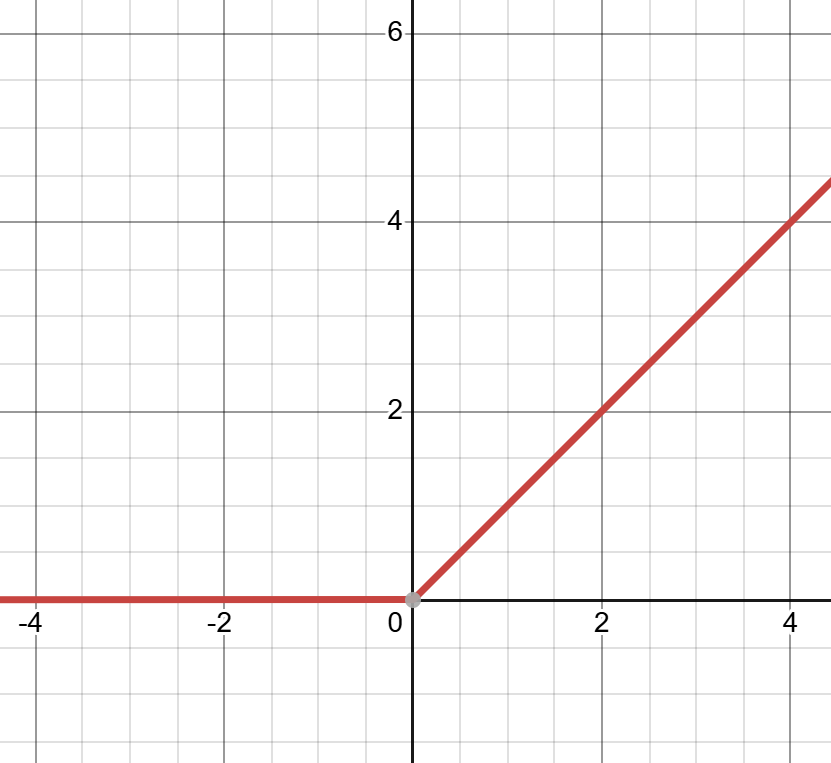
\includegraphics{images/image-0001.png}
\caption{ReLU 函数图像}
\end{figure}

这时候问题来了：

ReLU 看起来只是一种信息损失（把负数全变成0），为什么它能让深度神经网络从一个``傻傻的''线性网络，变成拥有各种强大功能的网络呢？

答案正是：非线性 (Non-linearity) 。

这个``拦住负数''的简单动作，引入了一个``折痕''或``关节''。想象一根直木棍（线性函数）。各种直线加加减减乘系数，得到的显然还是直线。但如果有了``关节''（ReLU函数），情况就完全不同了。

我们现在有四个线性函数：

\begin{figure}[htbp]
\centering
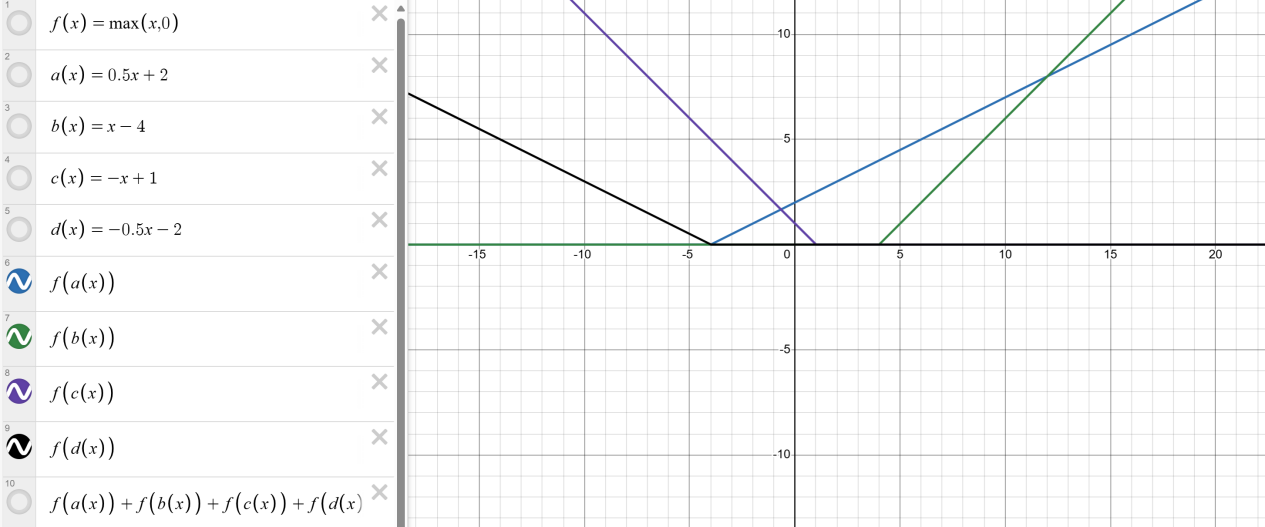
\includegraphics{images/image-0002.png}
\caption{ReLU 变换前的线性函数}
\end{figure}

分别经过ReLU函数（图中用f表示）后如下，可以发现每个函数经过ReLU函数时的``关节位置''和``伸展方向''不同：

\begin{figure}[htbp]
\centering
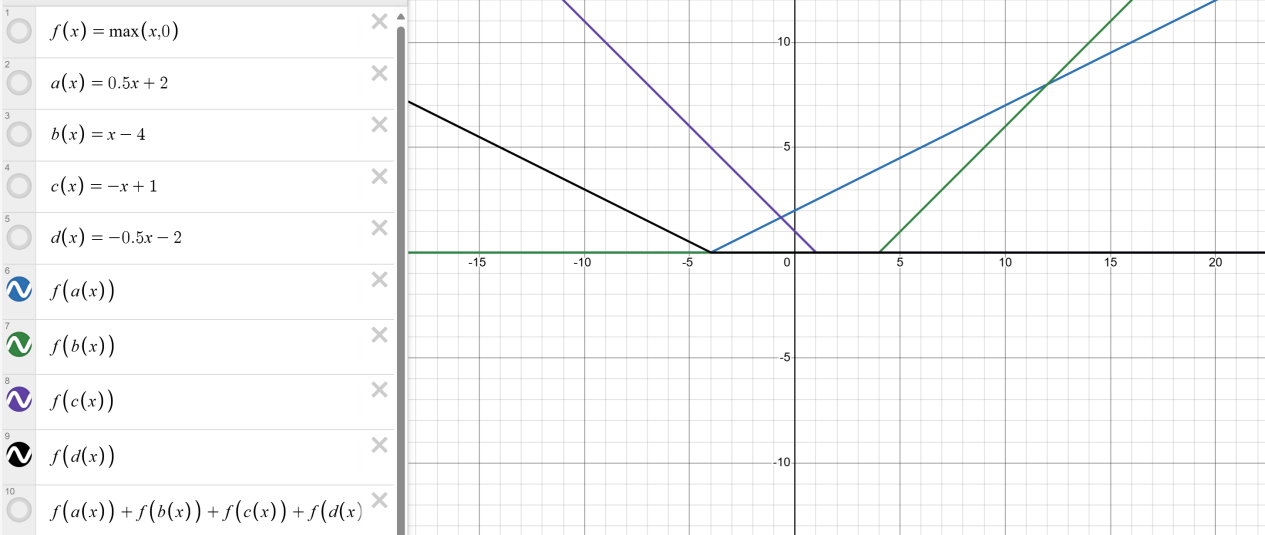
\includegraphics{images/image-0003.png}
\caption{ReLU 变换后的分段线性函数}
\end{figure}

再相加，每一个不同的``关节''都成为了新函数的``关节''：

\begin{figure}[htbp]
\centering
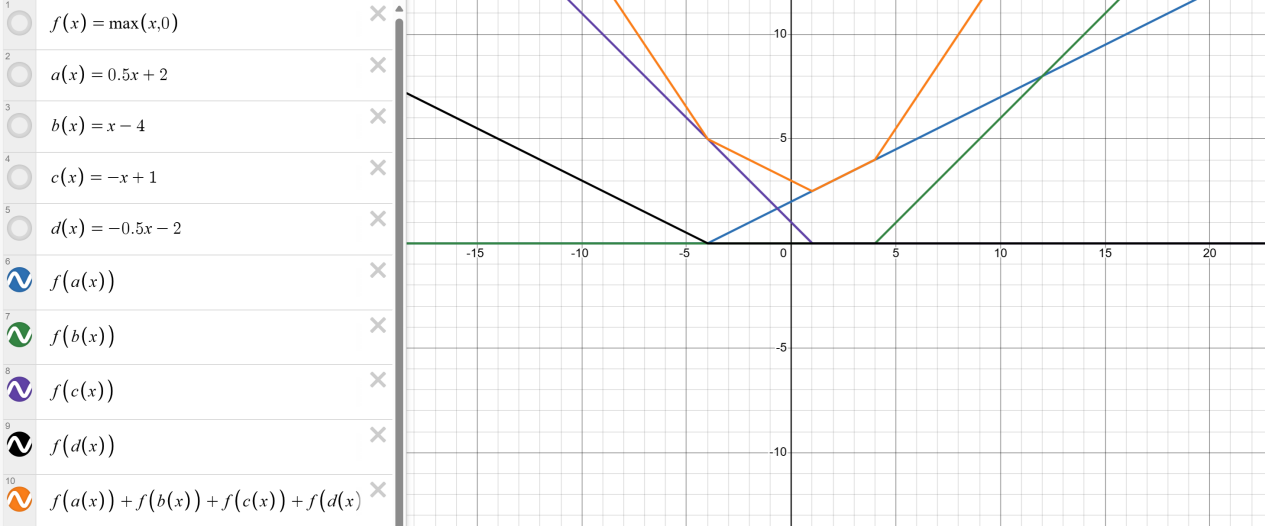
\includegraphics{images/image-0004.png}
\caption{多个 ReLU 函数相加得到更复杂的分段线性函数}
\end{figure}

这就是通用近似定理（Universal Approximation Theorem）的通俗理解：只要你有足够多的带``关节''（非线性激活函数）的神经元，理论上你可以``拼''出（拟合）宇宙中任何一个复杂的函数。

当然，``一刀切''地把负数全砍掉有时太粗暴了。万一负数信息也有用呢？于是研究者们发明了一些变种，比如 Leaky ReLU，它允许负数``泄露''一点点信息过去：f(x) = max(x, 0) + a*min(x, 0)，当a=0时，就变回了普通的ReLU。

\hypertarget{ux56dbux635fux5931ux51fdux6570}{%
\subsection{四、损失函数}\label{ux56dbux635fux5931ux51fdux6570}}

刚才我们搭建了一台由``师傅''（神经元）和``关节''（ReLU）组成的``函数机器''。它现在可以对输入x给出自己的输出y了。那么，我们怎么知道它输出的 \(y\) 是``好''还是``坏''呢？

就像考试需要``评分标准''一样，AI也需要一个``评分标准''来衡量它的预测结果和``标准答案''之间的差距。这个``评分标准''就是损失函数（Loss Function）。损失函数是一个``打分器''。把AI的全部参数丢进去，它会根据输入和输出算出一个损失值（Loss）。训练AI的唯一目标，就是通过不断调整参数，最终寻找到一组参数，让这个``损失值''变得最小，也就是它的输出最接近我们期望达到的目标，完美预测时的损失为0。在线性回归中，这组参数是可以算出解析解的，但在大部分问题中并不能（后续会讲优化参数的方法）。

回归问题中，最常用的损失函数是平方误差函数。当样本的预测值为 \(\hat{y}\)，其相应的真实标签为 \(y\) 时，平方误差可以定义为：

\[
Loss=\frac{1}{2}(\hat{y}-y)^2
\]

对于一个批量的 \(n\) 个样本，总损失为：

\[
Loss=\frac{1}{2}\sum_{i=1}^{n}(\hat{y}_i-y_i)^2
\]

这实际上就是最小二乘法。（常数不同没有本质差别，取1/2是为了让损失函数求导后常数系数为1，在后续计算梯度时更加方便）

高中课本告诉我们均方损失是因为绝对值函数没有那么良好的性质。但是我们为什么偏偏选择``平方''呢？

一方面，前面已经阐述过，它求导会得到 \(\hat{y}-y\) 这个简洁的项，可以让后续求解梯度更加方便。但是其实，均方损失的背后还有深刻的统计学含义。

我们假设AI的预测是准的，但现实中总会有一些随机的误差（也就是``噪声''），使得数据集中的数据并不完全符合它本应该符合的函数分布。我们假设这些``噪声''服从高斯分布（正态分布）。假设这个完全正确的AI的参数为θ，此时根据公式，输入x的时候，输出y的概率密度（在输出值连续的情况下，可以理解为输出值介于y和y+dy之间的概率除以dy）为：

\[
p(y \mid \mathbf{x};\theta)=\frac{1}{\sqrt{2\pi\sigma^2}}\exp\left(-\frac{(y-f(\mathbf{x};\theta))^2}{2\sigma^2}\right).
\]

我们希望这个概率越大越好，这就是``极大似然估计''，这里σ是高斯分布的系数。为了让这个概率最大，只需要让指数里的那个括号里的项最小，那一项正是参数为θ下的均方损失。

后续，我们还会介绍另一种损失函数------交叉熵损失函数。

\hypertarget{ux53c2ux8003ux6587ux732e}{%
\subsection{参考文献}\label{ux53c2ux8003ux6587ux732e}}

\begin{itemize}
\tightlist
\item
  Goodfellow, I., Bengio, Y., \& Courville, A. (2016). \href{https://www.deeplearningbook.org/}{Deep Learning}. MIT Press.
\item
  Cybenko, G. (1989). \href{https://doi.org/10.1007/BF02551274}{Approximation by superpositions of a sigmoidal function}. Mathematics of Control, Signals and Systems, 2, 303-314.
\item
  Glorot, X., Bordes, A., \& Bengio, Y. (2011). \href{https://proceedings.mlr.press/v15/glorot11a.html}{Deep Sparse Rectifier Neural Networks}. AISTATS 2011.
\end{itemize}

\clearpage

\hypertarget{ux68afux5ea6ux4e0bux964dux4e0eux53cdux5411ux4f20ux64ad}{%
\section{梯度下降与反向传播}\label{ux68afux5ea6ux4e0bux964dux4e0eux53cdux5411ux4f20ux64ad}}

\hypertarget{ux4e00ux68afux5ea6ux4e0bux964d}{%
\subsection{一、梯度下降}\label{ux4e00ux68afux5ea6ux4e0bux964d}}

\begin{enumerate}
\def\labelenumi{\arabic{enumi}.}
\tightlist
\item
  基本原理
\end{enumerate}

我们现在有了一台``机器''（神经网络），也知道如何给它``打分''（损失函数）。接下来的问题是：AI如何根据这个``分数''来``自我改进''呢？

想象一下，你（AI）站在一个n+1维的巨大山脉（``损失关于n维参数的曲面''）上，山上全是浓雾（全局函数无法直接求解得出）。你的目标是找到海拔最低的``山谷''（Loss最小值）。你看不见谷底在哪，只能往``下降最快''的方向走。

在数学上，梯度（Gradient）是一个向量，它的每一个值代表因变量（Loss）对每个自变量的偏导数值（可以理解为其他变量不变时，因变量对该自变量的导数，即因变量变化量/该自变量变化量的极限）：

\[
\nabla L = \left(\frac{\partial L}{\partial \theta_1}, \frac{\partial L}{\partial \theta_2}, \ldots, \frac{\partial L}{\partial \theta_n}\right)
\]

梯度指示的是参数发生改变时损失的增加量，而我们希望损失下降，所以会在梯度向量前面加一个负号，取它的反方向。对于一个有n个参数的模型，负梯度向量是一个集合了``n个方向陡峭程度''的``指令包''。如第一项代表``只改变θ1时，海拔（L）下降的快慢'' 。

\begin{figure}[htbp]
\centering
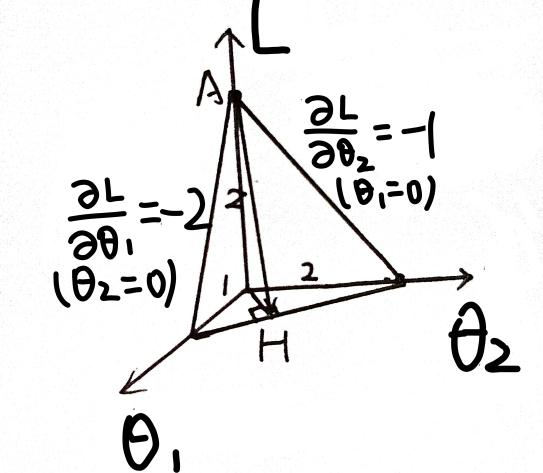
\includegraphics{images/image-0005.jpeg}
\caption{梯度下降方向示意图}
\end{figure}

比如上图中，只有两个参数，损失L是一个由两个输入决定的函数。损失L在θ1方向的``陡峭度''是-1，θ2方向的``陡峭度''是-2，负梯度向量就是(1, 2)。而``下降最快''的路径AH在参数空间（也就是图中的底面）上的投影OH（即``等高线最密集''的方向）的方向和负梯度向量(1, 2)相同。这也就说明了我们应该沿着负梯度方向下降。

\begin{enumerate}
\def\labelenumi{\arabic{enumi}.}
\setcounter{enumi}{1}
\tightlist
\item
  学习率调节
\end{enumerate}

我们知道了梯度改变的方向，那么改变多少呢？

一般我们会把负梯度向量乘以一个常数，它称为学习率。这个学习率是一个超参数，它自身无法通过梯度下降法来优化，只能人为调整好。下面两张图是从L轴看，如果学习率过大或过小，参数更新时会出现的问题。如果学习率太大，可能会出现``震荡''的情形，始终无法取到最低点，甚至适得其反；如果学习率太小，会导致步长太小，梯度下降需要的步数更多，计算量和计算开销更大。

\begin{figure}[htbp]
\centering
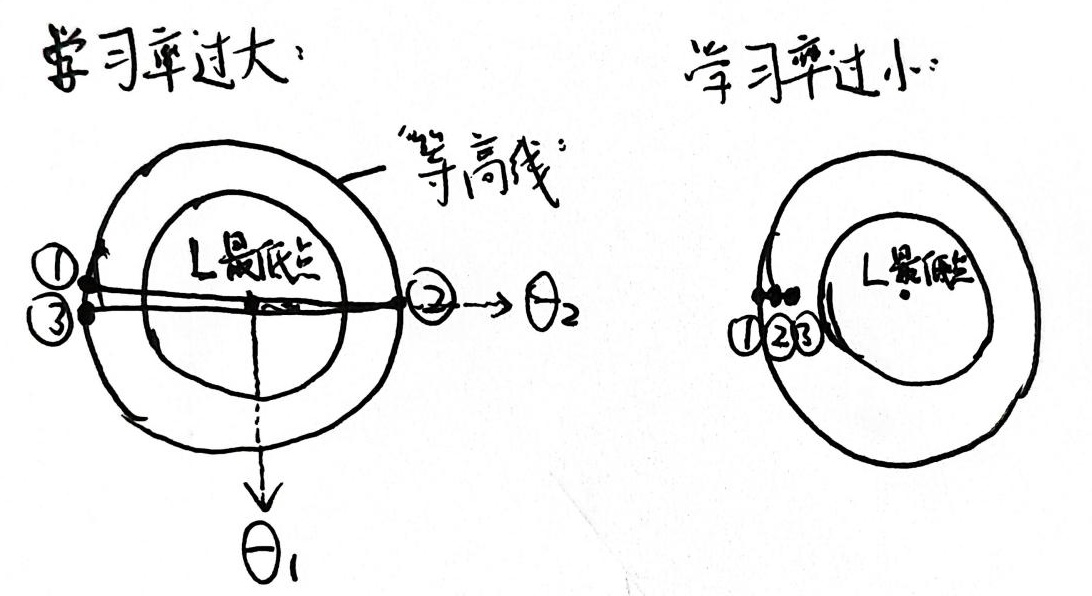
\includegraphics{images/image-0006.jpeg}
\caption{学习率过大或过小的影响}
\end{figure}

\begin{enumerate}
\def\labelenumi{\arabic{enumi}.}
\setcounter{enumi}{2}
\tightlist
\item
  小批量随机梯度下降
\end{enumerate}

我们知道了梯度下降，但是这里的Loss应该取谁的损失呢？

如果取所有样本的平均，不仅计算开销大，而且因为每一步取的都是相同样本的Loss对参数的函数，缺乏随机性，很容易``陷入''局部最小值，``出不来了''；如果只取一个样本，又随机性太大。因此，我们一般会把样本随机分为多个小批量（Mini-Batch），每次利用一个批量的数据计算Loss对各个参数的负梯度，进行梯度下降，这样就兼顾了准确性、适当的随机性和计算开销。

\hypertarget{ux4e8cux53cdux5411ux4f20ux64ad}{%
\subsection{二、反向传播}\label{ux4e8cux53cdux5411ux4f20ux64ad}}

我们已经知道，AI需要沿着负梯度方向这个``指令包''来下山。但一个关键问题悬而未决：在一个拥有数百万甚至数十亿参数的复杂神经网络中，如何高效地计算出这个包含损失函数对所有参数的梯度（即每个方向的``陡峭度''）的``指令包''呢？

反向传播是一种利用链式法则，从输出层开始，逐层向后（反向）计算损失函数对网络中每一个参数的偏导数的算法。我们可以把它理解为一个精妙的责任与误差分配系统。

\begin{enumerate}
\def\labelenumi{\arabic{enumi}.}
\tightlist
\item
  一个直观的比喻：生产线与责任追溯
\end{enumerate}

想象一个生产巧克力的工厂（神经网络）：输入可可粉、糖、牛奶等原材料（输入数据），经过混合、加热、搅拌、冷却、塑形等多层工序（网络层），输出一块成品巧克力（预测结果），质检品尝后给出评分，比如``太苦了''（计算损失）。现在发现巧克力太苦（损失很大），工厂需要改进。反向传播要解决的问题是：如何精确地知道每一道工序应该承担多少``责任''？是搅拌工序（某一中间层）没搅匀吗？还是加热工序（另一层）温度不对？或者说，根本就是采购的可可粉（输入数据）本身浓度太高？

它会进行精准的责任追溯：

质检员（损失函数）~首先确定最终产品``苦''的程度（损失L输出的梯度），回溯给最后的塑形工序：``你的产品太苦了，偏差量为xxx。''塑形工序收到反馈后想：``我本身只是塑形，苦味主要来自冷却工序传给我的半成品，而且根据我的工艺（激活函数），我对苦味的敏感度是这样的\ldots{}'' 于是它结合自己的``工艺特性''（本地梯度），计算出了对上一道工序（冷却工序）的责任指控，并把这个指控向后传递。这个过程逐层反向进行，每一层都根据后一层传来的``指控''和自身的``工艺说明书''（本地函数和其导数），计算出自己对问题的责任，并继续向更前端的工序追溯。最终，这个误差信号被传递到了最开始的原材料采购（输入层）~和每一道具体的工序。于是，每个环节都清楚地知道了：``哦，我需要为这个`苦'的结果负XX\%的责任。''

\begin{enumerate}
\def\labelenumi{\arabic{enumi}.}
\setcounter{enumi}{1}
\tightlist
\item
  数学表达
\end{enumerate}

这个``责任追溯''在数学上是通过微积分中的链式法则实现的。链式法则用于计算复合函数的导数。

假设一个简单的网络：输入层x -\textgreater{} 中间层h = f(w1\emph{x) -\textgreater{} 输出层y = g(w2}h) -\textgreater{} 损失L(y)

我们想求损失L关于第一个参数w1的梯度。根据链式法则：

\[
\frac{\partial L}{\partial w_1}=\frac{\partial L}{\partial y}\cdot\frac{\partial y}{\partial h}\cdot\frac{\partial h}{\partial w_1}
\]

反向传播的过程就是从上式右边向左计算：

\begin{enumerate}
\def\labelenumi{\arabic{enumi}.}
\tightlist
\item
  前向传播：先进行一次完整的从x到L的计算，记录下每一层的中间结果（h，y）。
\item
  反向计算：

  \begin{enumerate}
  \def\labelenumii{\alph{enumii}.}
  \tightlist
  \item
    首先计算 \(\frac{\partial L}{\partial y}\)（损失对输出的梯度）。
  \item
    然后，将这个梯度乘以 \(\frac{\partial y}{\partial h}\)（输出对中间层的梯度），得到 \(\frac{\partial L}{\partial h}\)（损失对中间层的梯度）。这就是将误差从输出层y传递到了中间层h。
  \item
    接着，将 \(\frac{\partial L}{\partial h}\) 乘以 \(\frac{\partial h}{\partial w_1}\)（中间层对参数w1的梯度），最终得到我们想要的 \(\frac{\partial L}{\partial w_1}\)。
    同理，L对w2的梯度也就是L对y的梯度乘以y对w2的梯度.计算出L对所有层的梯度后， 执行梯度下降即可。
  \end{enumerate}
\end{enumerate}

\hypertarget{ux4e09ux68afux5ea6ux6d88ux5931ux548cux68afux5ea6ux7206ux70b8}{%
\subsection{三、梯度消失和梯度爆炸}\label{ux4e09ux68afux5ea6ux6d88ux5931ux548cux68afux5ea6ux7206ux70b8}}

\hypertarget{ux4e00ux539fux56e0}{%
\subsubsection{（一）原因}\label{ux4e00ux539fux56e0}}

在反向传播中，为了计算靠近输入层的参数的梯度，我们需要将后面所有层的梯度连乘起来。对于一个L层的网络，损失对第一层权重 \(W^{[1]}\) 的梯度：

\[
\begin{aligned}
\frac{\partial L}{\partial W^{[1]}}
&=
\frac{\partial L}{\partial a^{[L]}}
\cdot
\frac{\partial a^{[L]}}{\partial z^{[L]}}
\cdot
\frac{\partial z^{[L]}}{\partial a^{[L-1]}} \\
&\quad \cdots
\cdot
\frac{\partial a^{[2]}}{\partial z^{[2]}}
\cdot
\frac{\partial z^{[2]}}{\partial a^{[1]}}
\cdot
\frac{\partial a^{[1]}}{\partial z^{[1]}}
\cdot
\frac{\partial z^{[1]}}{\partial W^{[1]}} .
\end{aligned}
\]

在深层网络中，如果其中大部分项的绝对值~小于1，那么连乘的结果会指数级地趋近于0，导致参数更新的幅度变得极小，网络的前面层几乎停止学习，参数更新微不足道。深度网络退化为一个只有后面几层在学习的浅层网络，无法发挥深度模型的表征能力。训练过程变得极其缓慢，甚至完全停滞。

反之，如果大部分项的绝对值~大于1，结果则会指数级地增长到无穷大，导致权重更新的幅度变得极大。参数更新步长巨大且不稳定，导致损失函数剧烈震荡，无法收敛。模型参数可能变成NaN（非数字），因为更新的值超出了计算机的浮点数表示范围。模型完全无法学习到有意义的模式。

\hypertarget{ux4e8cux89e3ux51b3ux65b9ux6848}{%
\subsubsection{（二）解决方案}\label{ux4e8cux89e3ux51b3ux65b9ux6848}}

\begin{enumerate}
\def\labelenumi{\arabic{enumi}.}
\item
  激活函数选择：使用x＞0时导数恒为1的ReLU函数，而不是在x很大或很小时导数趋于0的Sigmoid函数。
\item
  参数初始化技巧：后续会介绍。
\item
  批量规范化：强制将每一层的输入拉回到标准正态分布，以让该层最终整体的梯度尽量接近1。
\item
  模型架构设计：如ResNet，通过``输出=x+f(x)''的设计（x为输入，f为模型层），建立一条从输入x``直达''输出的``梯度高速公路''，让梯度可以无损地直接流向较浅的层，从根本上解决了深层网络（如上百层的 ResNet）的梯度消失问题。
\item
  梯度裁剪：针对梯度爆炸，可以在更新权重前，检查梯度的范数（梯度向量的长度）。如果超过设定的阈值，就对梯度在各个方向进行等比例缩放，使其范数（长度）在阈值以内：
\end{enumerate}

如果 \(\lVert g\rVert > \text{threshold}\)，则：

\[
g\leftarrow \frac{\text{threshold}}{\lVert g\rVert}\cdot g
\]

\hypertarget{ux53c2ux8003ux6587ux732e-1}{%
\subsection{参考文献}\label{ux53c2ux8003ux6587ux732e-1}}

\begin{itemize}
\tightlist
\item
  Rumelhart, D. E., Hinton, G. E., \& Williams, R. J. (1986). \href{https://doi.org/10.1038/323533a0}{Learning representations by back-propagating errors}. Nature.
\end{itemize}

\clearpage

\hypertarget{ux8fc7ux62dfux5408}{%
\section{过拟合}\label{ux8fc7ux62dfux5408}}

\hypertarget{ux4e00ux8fc7ux62dfux5408ux4e0eux6b20ux62dfux5408}{%
\subsection{一、过拟合与欠拟合}\label{ux4e00ux8fc7ux62dfux5408ux4e0eux6b20ux62dfux5408}}

在训练时，我们只能看到模型在训练集上的Loss，我们希望它变小。但是这是可以``作弊''的：如果模型单纯``记住''所有数据，它的训练Loss为零，但在真实世界中毫无用处。比如一个医疗模型，部署时模型需要判断从未见过的患者。只有当模型真正发现了一种泛化模式时，才会作出有效的预测。我们如何才能确定模型是真正发现了一种泛化的规律，而不是简单地记住了数据呢？

\begin{enumerate}
\def\labelenumi{\arabic{enumi}.}
\tightlist
\item
  训练误差和泛化误差
\end{enumerate}

训练误差（Training Error）：模型在训练数据集上计算得到的误差。

泛化误差（Generalization Error）：模型应用在同样从原始样本的分布中抽取的无限多数据样本时，模型误差的期望。

困难在于，泛化误差是一个理想化的数值，我们永远无法准确计算（因为我们无法获取无限的数据）。在实际中，我们只能通过将模型应用于一个独立的测试集来估计泛化误差。

\begin{enumerate}
\def\labelenumi{\arabic{enumi}.}
\setcounter{enumi}{1}
\tightlist
\item
  过拟合
\end{enumerate}

所谓``过拟合''，就是训练误差很低，但泛化误差很高的情况。

过拟合可以用大家熟悉的一个例子来解释：大家在备战高考的时候，在模拟考试里取得好成绩并不能保证在高考时考好。例如，模拟考试经常一味模仿上一年的高考题，如果学生就把这种题目的套路和手法做得很熟，却会在面对高考的新题时无所适从，这就是``过拟合''。备战高考的学生在做模拟题时，只有理解和掌握其背后可迁移的普遍思想方法，才能在面对高考的新题时游刃有余；同样的，对于模型而言，只有学习到数据背后的泛化规律，才能进行有效的预测。

再比如一个小学生，如果理解了公式原理（如1+1=2），即使考试题目将数字从1换成了5，他依然能计算出正确答案。这意味着他的``泛化误差''很低。过拟合的学习则像一个记忆力超群的学生，把练习册上每一道题的答案都背了下来，在平时练习里能拿满分（训练误差为 0），到了期末考试，题目稍微变动一点，出现一个他没见过的数字（比如9），他就完全不会了。

\begin{enumerate}
\def\labelenumi{\arabic{enumi}.}
\setcounter{enumi}{2}
\tightlist
\item
  过拟合与模型复杂度的关系
\end{enumerate}

模型复杂性由什么构成是一个复杂的问题。通常对于神经网络，参数越多、取值范围越大、训练时间越长，模型就越复杂。为了直观地解释``模型复杂性''如何导致过拟合，我们来看一个经典的多项式拟合例子。

假设真实世界的数据规律是一个简单的二次函数（抛物线），再加上一点点观测时的随机误差（噪声）：y=ax\^{}2+bx+c+epsilon。如果我们使用一个过于复杂的模型，比如一个9次多项式y = w\_9x\^{}9 + w\_8x\^{}8 + \ldots{} + w\_1x + w\_0（拥有10个参数）来拟合这些数据，因为模型有10个自由度，它有足够的能力去扭曲自己，好比我们允许模型使用一把极度柔软、可以随意弯曲的尺子去连接纸上的点，它会强行穿过每一个因为测量误差而偏离真实轨迹的样本点。

为了穿过那些不规则分布的噪声点，模型被迫让高次项的系数（如w\_9）变得非常大。对于高次项x\^{}9，输入x只要有极其微小的变化，输出值y就会发生巨大的爆炸式变化。最终拟合出来的函数曲线不再是一条平滑的抛物线，而变成了一条上下翻飞、剧烈震荡的``心电图''。虽然它完美穿过了所有训练点，但在测试点上，这种剧烈的震荡会导致预测值非常离谱（9次函数和2次函数随机取点相差大概率是非常大的）。

而欠拟合则相反，如用一条直线拟合二次函数，模型灵活度太低，无法把握数据间的规律，效果不好。

\hypertarget{ux4e8cux589eux52a0ux8badux7ec3ux6570ux636eux91cf}{%
\subsection{二、增加训练数据量}\label{ux4e8cux589eux52a0ux8badux7ec3ux6570ux636eux91cf}}

过拟合意味着模型复杂度显著大于数据量。对于相同的模型，训练数据集中的样本越少，我们就越有可能（且更严重地）过拟合；对于相同量的数据，模型复杂度越大，越可能过拟合。因此，我们可以增大训练数据量，或降低模型复杂度。这里探讨增大数据量。

这里涉及到一个核心假设：独立同分布假设。我们假设训练数据和测试数据都是从相同的概率分布中独立提取的。如果数据分布发生变化（例如，用大学生的照片训练人脸识别，去识别养老院的老人），模型就会失效。

即便分布一致，如果数据量太少（例如只有几千张图片），复杂的深度学习模型很容易就能``记住''所有图片，而不是学习特征。深度学习目前的繁荣，很大程度上归功于海量数据集的出现，使得我们能够训练复杂的模型而不过度过拟合。

在垂直任务中，我们的真实数据往往非常少或非常昂贵。如在医学影像（如CT或MRI）中，要诊断一种罕见的癌症。我们可能只有几百张（甚至几十张）带标签的``阳性''图像。此时为了解决过拟合，可以进行以下处理：

\begin{enumerate}
\def\labelenumi{\arabic{enumi}.}
\item
  迁移学习：利用已经在大数据集上预训练好的大模型，在这些小型数据集上进行微调。
\item
  对已有数据进行变换：对于图像而言，就是旋转、裁剪、缩放、翻转、平移、添加噪声、改变对比度或亮度等。
\item
  利用VAE（变分自编码器）：在编码-解码的过程中，一个 VAE 的编码器输出一个概率分布，解码器不是从一个``点''来重建，而是从这个``模糊区域''中随机采样一个点来进行重建。
\item
  利用GAN生成：我们可以训练一个基于生成器-判别器架构的GANs模型（比如一个变种的DCGAN或WGAN），判别器以这几百张真实癌症图像的分布为参考基准。一旦训练完成，这个GANs的生成器就可以从随机噪声开始，生成成千上万张看起来逼真、但又与原始图像不完全相同的``假''癌症图像。
\end{enumerate}

\hypertarget{ux4e09ux6a21ux578bux6b63ux5219ux5316ux964dux4f4eux6a21ux578bux590dux6742ux5ea6ux89c1ux540eux7eedux5173ux4e8eux6a21ux578bux6b63ux5219ux5316ux7684ux5185ux5bb9}{%
\subsection{三、模型正则化（降低模型复杂度，见后续关于模型正则化的内容）}\label{ux4e09ux6a21ux578bux6b63ux5219ux5316ux964dux4f4eux6a21ux578bux590dux6742ux5ea6ux89c1ux540eux7eedux5173ux4e8eux6a21ux578bux6b63ux5219ux5316ux7684ux5185ux5bb9}}

\hypertarget{ux53c2ux8003ux6587ux732e-2}{%
\subsection{参考文献}\label{ux53c2ux8003ux6587ux732e-2}}

\begin{itemize}
\tightlist
\item
  Aston Zhang, Zachary C. Lipton, Mu Li, Alexander J. Smola. (2023). \href{https://zh.d2l.ai/}{《动手学深度学习》}. Cambridge University Press.
\end{itemize}

\clearpage

\hypertarget{ux4ea4ux53c9ux71b5ux635fux5931ceux4e0esoftmaxux56deux5f52}{%
\section{交叉熵损失（CE）与Softmax回归}\label{ux4ea4ux53c9ux71b5ux635fux5931ceux4e0esoftmaxux56deux5f52}}

\hypertarget{ux4e00ux4ea4ux53c9ux71b5ux635fux5931ux51fdux6570cross-entropyce}{%
\subsection{一、交叉熵损失函数（Cross Entropy,CE）}\label{ux4e00ux4ea4ux53c9ux71b5ux635fux5931ux51fdux6570cross-entropyce}}

在分类任务中，例如要看一张图，判断它是``猫''、``狗''还是``鸟''。AI会给出一个``概率分布''，比如q={[}猫: 0.7, 狗: 0.2, 鸟: 0.1{]}，标准答案： 真实答案也是一个概率分布，p={[}猫: 1, 狗: 0, 鸟: 0{]}。这时用MSE来量q\_i和p\_i之间的``距离''就非常不合适了。下面我们引入信息论中的``信息熵''和``交叉熵''概念。

信息论认为，信息是用来消除随机不确定性的东西。信息量取决于不确定性，它可以被理解为一种``惊讶度''，或者说描述这个事件发生的所有可能性所需要的编码数：

如果一个事件必然发生（概率~P=1），它不需要任何编码信息，你已经知道了它必然发生，因此毫不惊讶，惊讶度为~-log₂(1) = 0比特。

如果一个事件有25\%的概率发生（P=0.5），这个事件的可能性等同于在00、01、10、11四个2位数编码中随机选择一个，在事件最终发生的那一刻，你获得了2比特的信息，有一些惊讶，惊讶度是~-log₂(0.25) = 2比特。

如果一个事件非常罕见（概率~P -\textgreater{} 0），惊讶度趋近于无穷大。在事件最终发生的那一刻，你极度惊讶。

对于一个离散的概率分布P，假设共有n种可能发生的事件，概率分别为(i=1,\ldots,n)，则信息量，或者说应该分配的编码数的期望为.

在机器学习中，我们有一个真实的分布~P（数据的真实标签），和一个模型预测的分布~Q。我们想知道这两个分布之间有多``不同''。KL散度，也称为相对熵，就是用来衡量用一个近似分布~Q去描述真实分布~P时，所产生的信息损耗。

从P到Q的KL散度定义为：

\[
D_{\mathrm{KL}}(P \parallel Q)=\sum_i p(i)\log\left(\frac{p(i)}{q(i)}\right)
\]

其中表示在真实概率为~p(i)的事件上，用~q(i)来描述它所产生的``信息差异''或``惊讶程度''。KL散度是将所有事件上的这种``信息差异''用真实概率p(i)~进行加权平均，是一个恒非负的函数，当且仅当P、Q两分布完全相同时值为0。

进一步地：

\[
\begin{aligned}
D_{\mathrm{KL}}(P \parallel Q)
&=\sum_i p(i)\log p(i)-\sum_i p(i)\log q(i)\\
&=H(P,Q)-H(P)
\end{aligned}
\]

H(P)是真实分布的信息熵，在分类任务中不变。H(P,Q)就是交叉熵，定义为：

\[
H(P,Q)=-\sum_i p(i)\log q(i)
\]

由于我们的目标是最小化 \(D_{\mathrm{KL}}(P\parallel Q)\)，而 \(D_{\mathrm{KL}}(P\parallel Q)=H(P,Q)-\mathcjk{常数}\)，那么：

\[
\min D_{\mathrm{KL}}(P\parallel Q)\Longleftrightarrow \min H(P,Q)
\]

在监督学习中，真实分布P是确定的值（有真实标签），与模型参数也无关。此时，用交叉熵来代替KL散度在代码上更简洁且不易出现log0错误。

从编码的角度，我们可以把交叉熵损失函数理解为是在用估计的概率分布进行编码，而事件服从真实分布，此时所需的平均编码数期望。

对于分类任务，为0或1（且只有一个值为1），且等于对应的标签值0或1，因此交叉熵损失可以写成为1时，若趋于0，快速增长，相当于只关心应该分入的那一类算出的概率值和1的接近程度（也就是那个，表示应该分入的那一类算出的概率值），不关心其他类。

对于一个批量的样本（如LLM一次性生成n个token），交叉熵损失函数取n个样本的均值.它可以被视为表达n个样本的``平均信息量''。进一步拓展：交叉熵损失函数取指数后，就可以视为整个序列的困惑度（``生成该序列时，每次平均从几个token里选一个''）。困惑度的n次方的倒数就是生成该序列的联合概率。

那么，为什么不使用均方损失呢？

\begin{enumerate}
\def\labelenumi{\arabic{enumi}.}
\item
  理论不符： MSE 衡量的是两个数值向量之间的欧氏距离。而交叉熵衡量的是两个概率分布之间的信息论距离。分类任务的本质是拟合概率分布，而非拟合特定数值。
\item
  梯度消失：以二分类（Sigmoid）为例：当我们计算交叉熵损失函数对分类常用的 Sigmoid 激活函数输入z的梯度时，推导结果极其优美：
\end{enumerate}

\[
\frac{\partial L_{\mathrm{BCE}}}{\partial z}=\hat{y}-y
\]

梯度大小正比于预测值与真实值之间的误差，误差越大，梯度更新越快，这是合理的。但如果使用MSE：

\[
\frac{\partial L_{\mathrm{MSE}}}{\partial z}=(\hat{y}-y)\cdot\sigma'(z)
\]

其中：

\[
\sigma'(z)=\sigma(z)(1-\sigma(z))=\hat{y}(1-\hat{y})
\]

梯度中多了一项 sigma'(z)。当 Sigmoid 函数的输出y\_hat趋近于0或1时，sigma'(z)这一项会趋近于0。 灾难在于：当模型非常自信地预测错误时（例如y\_hat=0.01），sigma'(z)几乎为0，模型明明错得离谱，却无法快速学习（梯度消失），导致训练极其缓慢或卡在局部最优。

\hypertarget{ux4e8csoftmaxux56deux5f52}{%
\subsection{二、Softmax回归}\label{ux4e8csoftmaxux56deux5f52}}

例如多分类问题，需要输出n个可能类别分别的概率，故要把原来该神经元输出的在实数范围内的logits值（如zi）变为e\textsuperscript{zi/(e}z1+\ldots+e\^{}zn)才能作为概率。好处：突出最高值，符合分类问题特性；归一化为0到1之间概率。运用交叉熵损失时：

由于 softmax 和相关的损失函数很常见，因此我们需要更好地理解它的计算方式。将 \(l(\mathbf{y},\hat{\mathbf{y}})\) 代入损失函数，利用 softmax 的定义，可以得到：

\[
\begin{aligned}
l(\mathbf{y},\hat{\mathbf{y}})
&=-\sum_{j=1}^{q}y_j\log\frac{\exp(o_j)}{\sum_{k=1}^{q}\exp(o_k)}\\
&=\sum_{j=1}^{q}y_j\log\sum_{k=1}^{q}\exp(o_k)-\sum_{j=1}^{q}y_jo_j\\
&=\log\sum_{k=1}^{q}\exp(o_k)-\sum_{j=1}^{q}y_jo_j
\end{aligned}
\]

考虑相对于任何未规范化预测 \(o_j\) 的导数，可以得到：

\[
\partial_{o_j}l(\mathbf{y},\hat{\mathbf{y}})
=\frac{\exp(o_j)}{\sum_{k=1}^{q}\exp(o_k)}-y_j
=\mathrm{softmax}(\mathbf{o})_j-y_j
\]

换句话说，导数是 softmax 模型分配的概率与实际发生情况（由独热标签向量表示）之间的差异。

也就是说，在各个方向上的梯度（下降速率）的比值就是每个方向预测值和实际值之差的比值，如模型预测概率{[}0.1, 0.7, 0.2{]}~，真实标签{[}0, 1, 0{]}~，计算出的梯度就是{[}0.1-0, 0.7-1, 0.2-0{]}。均方损失（对应噪声满足高斯分布）也满足这一特点。

实际计算时：

回想一下，softmax 函数为：

\[
\hat{y}_j=\frac{\exp(o_j)}{\sum_k\exp(o_k)}
\]

其中 \(\hat{y}_j\) 是预测的概率分布，\(o_j\) 是未规范化预测 \(\mathbf{o}\) 的第 \(j\) 个元素。如果 \(o_k\) 中的一些数值非常大，那么 \(\exp(o_k)\) 可能大于数据类型允许的最大数字，即上溢（overflow）。为避免这个问题，可以在继续 softmax 计算之前，先从所有 \(o_k\) 中减去 \(\max(o_k)\)。每个 \(o_k\) 按常数移动不会改变 softmax 的返回值：

\[
\begin{aligned}
\hat{y}_j
&=\frac{\exp(o_j-\max(o_k))\exp(\max(o_k))}
{\sum_k\exp(o_k-\max(o_k))\exp(\max(o_k))}\\
&=\frac{\exp(o_j-\max(o_k))}
{\sum_k\exp(o_k-\max(o_k))}
\end{aligned}
\]

尽管我们要计算指数函数，但最终在计算交叉熵损失时会取它们的对数。通过将 softmax 和交叉熵结合在一起，可以直接使用 \(o_j-\max(o_k)\)，避免反向传播过程中可能困扰我们的数值稳定性问题：

\[
\begin{aligned}
\log(\hat{y}_j)
&=\log\left(\frac{\exp(o_j-\max(o_k))}
{\sum_k\exp(o_k-\max(o_k))}\right)\\
&=\log(\exp(o_j-\max(o_k)))
-\log\left(\sum_k\exp(o_k-\max(o_k))\right)\\
&=o_j-\max(o_k)-\log\left(\sum_k\exp(o_k-\max(o_k))\right)
\end{aligned}
\]

\hypertarget{ux4e09ux4e8cux5143ux4ea4ux53c9ux71b5ux635fux5931bce}{%
\subsection{三、二元交叉熵损失（BCE）}\label{ux4e09ux4e8cux5143ux4ea4ux53c9ux71b5ux635fux5931bce}}

\begin{enumerate}
\def\labelenumi{\arabic{enumi}.}
\tightlist
\item
  二元交叉熵的数学表达
\end{enumerate}

当分类问题只有两个类别（真或假）可以二选一时，假设为真的实际概率为p，预测为真的概率为q，实际数据标签（真为1，假为0）为y，则真实二元交叉熵的公式为-p\emph{logq-(1-p)}log(1-q)，又y=p，也可写成-y\emph{logq-(1-y)}log(1-q).

\begin{enumerate}
\def\labelenumi{\arabic{enumi}.}
\setcounter{enumi}{1}
\tightlist
\item
  模型给出预测概率q的方式
\end{enumerate}

当只有两个类别时，我们就不再需要输出多个logits值后用Softmax了，而是只需要一个logit，用sigmoid函数得到为其中某一类（如选择``是''）的概率，再用二元交叉熵。事实上可以证明这种操作就是Softmax的一种特殊情况：

对于两个类别，Softmax输出为：

\[
p_0=\frac{e^{z_0}}{e^{z_0}+e^{z_1}},\qquad
p_1=\frac{e^{z_1}}{e^{z_0}+e^{z_1}}
\]

只关心第二个类别的概率 \(p_1\)，并定义 \(z=z_1-z_0\)：

\[
p_1=\frac{e^{z_1}}{e^{z_0}+e^{z_1}}
=\frac{1}{1+e^{-(z_1-z_0)}}
=\sigma(z_1-z_0)
\]

所以二元Softmax可以简化为Sigmoid函数，其中输入是两类logits的差值。

\begin{enumerate}
\def\labelenumi{\arabic{enumi}.}
\setcounter{enumi}{2}
\tightlist
\item
  BCE在多标签分类中的运用
\end{enumerate}

由于Softmax函数只适用于``n选一''式的``单选''分类，如果我们需要同时将一个对象分到多个类别（如给蛋白质加各种功能标签），进行``多选''分类，Softmax就不适用了。这时我们可以把任务看成有很多（样本，类别）组合，对于每一个组合，都分别判断该对象是否分入该类别。此时，交叉熵损失先按所有（样本，类别）组合加起来，然后按组合总数取平均。

多标签交叉熵损失的代码实现：

\begin{verbatim}
import torch

import torch.nn as nn

# 假设批次大小=2，类别数=3

logits = torch.tensor([[1.2, -0.5, 0.8],[-0.3, 1.5, -1.0]]) #模型输出的原始值（未经过激活函数）

targets = torch.tensor([[1, 0, 1], [0, 1, 0]], dtype=torch.float) #真实标签，这里用0和1表示每个样本是否属于某个类别

# 使用BCEWithLogitsLoss（默认reduction='mean'即取平均模式）

criterion = nn.BCEWithLogitsLoss()

loss = criterion(logits, targets)

print(f"损失值: {loss.item()}")

# 手动验证计算过程

sigmoid_outputs = torch.sigmoid(logits)

bce_per_element = - (targets * torch.log(sigmoid_outputs) +

(1 - targets) * torch.log(1 - sigmoid_outputs)) #相同形状的矩阵，Pytorch执行按元素乘法

print(f"每个(样本,类别)的损失:\n{bce_per_element}")

total_loss = bce_per_element.sum()

num_elements = bce_per_element.numel()  # N × C = 2 × 3 = 6

manual_loss = total_loss / num_elements

print(f"手动计算的平均损失: {manual_loss.item()}")
\end{verbatim}

\hypertarget{ux53c2ux8003ux6587ux732e-3}{%
\subsection{参考文献}\label{ux53c2ux8003ux6587ux732e-3}}

\begin{itemize}
\tightlist
\item
  Aston Zhang, Zachary C. Lipton, Mu Li, Alexander J. Smola. (2023). \href{https://zh.d2l.ai/}{《动手学深度学习》}. Cambridge University Press.
\end{itemize}

\clearpage


% 神经网络训练的常用方法
\hypertarget{ux795eux7ecfux7f51ux7edcux8badux7ec3ux7684ux5e38ux7528ux65b9ux6cd5}{%
\chapter{神经网络训练的常用方法}\label{ux795eux7ecfux7f51ux7edcux8badux7ec3ux7684ux5e38ux7528ux65b9ux6cd5}}

\hypertarget{ux6a21ux578bux6b63ux5219ux5316}{%
\section{模型正则化}\label{ux6a21ux578bux6b63ux5219ux5316}}

\hypertarget{ux4e00ux6a21ux578bux6b63ux5219ux5316ux7684ux6570ux5b66ux57faux7840}{%
\subsection{一、模型正则化的数学基础}\label{ux4e00ux6a21ux578bux6b63ux5219ux5316ux7684ux6570ux5b66ux57faux7840}}

\begin{enumerate}
\def\labelenumi{\arabic{enumi}.}
\tightlist
\item
  偏差与方差
\end{enumerate}

偏差大：预测数据均值偏离实际均值，欠拟合。

方差大：预测数据学到了太多噪声，过拟合。

\begin{enumerate}
\def\labelenumi{\arabic{enumi}.}
\setcounter{enumi}{1}
\tightlist
\item
  贝叶斯公式
\end{enumerate}

先验概率p(A)是对一个事件概率如疾病发病率的初始估计；

p(B\textbar A)是A发生的情况下，能观测到证据B如阳性的概率；

p(B)是A发生与否两种情况下观测到证据B的概率和；

p(A\textbar B)是观测到证据B的情况下，对概率估计的进一步更新。

\begin{enumerate}
\def\labelenumi{\arabic{enumi}.}
\setcounter{enumi}{2}
\tightlist
\item
  贝叶斯公式在正则化中的应用
\end{enumerate}

（1）基本量

p(参数)：先验项，也就是对``参数值为X''这一事件发生概率的初始估计，若无正则化项则可忽略本项。

p(输出\textbar 参数)：这里的``输出''指的是，在已知``参数值为X''的条件下，出现输出Y的概率；损失函数最小时，p(输出\textbar 参数)最大（最大似然估计得到）。

p(输出)：尝试过所有参数后，得到该输出Y的平均概率，一般认为是常数（从可输出的词的列表中完全随机抽取）。

（2）基本解释

p(参数\textbar 输出)=p(输出\textbar 参数)\emph{p(参数)/p(输出)，或者说认为p(参数\textbar 输出)正比于p(输出\textbar 参数)}p(参数)，我们的目的是在给定输出的情况下，求出最可能产生这样输出的参数，也就是p(参数\textbar 输出)最大，在设计损失函数时，会把这种情形定义为损失函数最小（如loss=-logp(参数\textbar 输出)），一轮轮训练中通过梯度下降一步步接近该参数组合，每次训练的过程就是把参数初始概率分布变成考虑输出后的概率分布，并通过梯度下降让参数接近概率最大似然估计的参数值。

（3）正常情况

没有加入正则化项时，我们对p(参数)没有任何事先估计【初始权重值从高斯分布取样是为了能进行梯度操作而不至于全0，仅为优化起点，不代表先验估计】，这时p(参数\textbar 输出)正比于p(输出\textbar 参数)，也就是我们认为，当某个给定参数的模型最可能产生某个输出时，想要让另一个模型实现该输出的最好方法就是拟合该模型的参数。

（4）过拟合

训练时有时会落入一个p(输出\textbar 参数)很大的参数组合，但其实出现了过拟合，在测试集中p(输出\textbar 参数)反而小【注意计算贝叶斯后验不能用测试集，只能用训练集，原因前面讲过】，为了我们抑制过拟合，必须手动调整p(参数)的分布，让p(参数\textbar 输出)最大的情形同时受训练时得出正确输出概率p(输出\textbar 参数)和先验分布p(参数)的影响。

（5）加入正则化后

在loss中加入正则化项，也就等价于通过控制初始概率分布函数p(参数)，使其不为定值，从而在估计中加入我们的额外偏好，p(输出\textbar 参数)大不一定代表loss小（如一些正则化项会给予复杂模型惩罚），让包含实现对参数最终分布的调整。

\hypertarget{ux4e8cl2ux6b63ux5219ux5316ux6743ux91cdux8870ux51cf}{%
\subsection{二、L2正则化（权重衰减）}\label{ux4e8cl2ux6b63ux5219ux5316ux6743ux91cdux8870ux51cf}}

即给损失函数加上``lamda\emph{1/2}参数平方和''项。lamda为正则化强度；1/2是为了在求正则项关于参数向量W的梯度时求导等于lamda*W而没有其他系数。

概率本质：由前面损失函数是取log得到的可知，p(参数)其实就是该参数下的高斯函数的值，等价于高斯先验，默认各参数接近0的概率大。

收敛方式：由于在0附近导数约为0，接近0时收敛极慢（收敛速度趋于0），一般不会收敛到0；但不会出现很大的参数（惩罚比L1大）。

对减小模型复杂度的作用：

（1）所有参数向零收缩，显著削弱高阶项，类似于限制多项式中高阶项系数。

（2）避免特征共线性带来的权重抵消问题（这种情形的惩罚值会很大）。

权重抵消效应的产生机制：

\begin{enumerate}
\def\labelenumi{\arabic{enumi}.}
\tightlist
\item
  参数解的不确定性
\end{enumerate}

当特征高度相关时（如 \(X_1\approx kX_2\)），模型无法区分每个特征的独立贡献。例如：

\begin{itemize}
\tightlist
\item
  真实关系：\(Y=2X_1+3X_2\)。
\item
  若 \(X_1\) 与 \(X_2\) 强相关（如 \(X_2\approx 0.5X_1\)），则以下解均可能成立：\(Y=4X_1+0\cdot X_2\)、\(Y=0\cdot X_1+6X_2\)、\(Y=5000X_1-4998X_2\)。
\end{itemize}

其中最后一种情况就是权重抵消：\(X_1\) 和 \(X_2\) 的系数符号相反且绝对值极大，它们的贡献相互抵消。最终组合结果仍接近真实值，但单个系数的可解释性较差。

\begin{enumerate}
\def\labelenumi{\arabic{enumi}.}
\setcounter{enumi}{1}
\tightlist
\item
  梯度更新的不稳定性
\end{enumerate}

在梯度下降优化过程中，高度相关特征的梯度方向可能冲突。若特征 \(X_1\) 和 \(X_2\) 相关且量级差异大（如 \(X_2=100X_1\)），则权重 \(w_2\) 的微小变化会导致 \(w_1\) 剧烈震荡，最终可能收敛到 \(w_1\) 为负、\(w_2\) 为正的抵消状态。

权重抵消效应会带来三类影响：

\begin{enumerate}
\def\labelenumi{\arabic{enumi}.}
\item
  模型可解释性降低。例如在房价预测中，若``房间数量''和``房间数量平方''同时作为特征，模型可能赋予前者正权重、后者负权重，导致``房间数量增加反而降低房价''的反常误读。
\item
  参数估计方差增大。共线性会使权重方差膨胀，样本中的微小扰动可能导致系数剧烈波动，使模型稳定性下降。
\item
  特征重要性失真。在线性模型中，权重符号和大小常用于判断特征与目标的关系，权重抵消可能使实际正相关的特征在模型中表现为负相关。
\end{enumerate}

其他好处：避免梯度爆炸，避免矩阵病态。

\hypertarget{ux4e09l1ux6b63ux5219ux5316}{%
\subsection{三、L1正则化}\label{ux4e09l1ux6b63ux5219ux5316}}

给损失函数加上``lamda*参数绝对值和''项，等价于对参数的初始估计为拉普拉斯先验，由于一次函数处处斜率相等，部分参数会被归零（L2在参数接近0的时候梯度也接近0，参数再向0的更新几乎停滞），剩余参数接近0的程度没有L2那么大（L2对偏离较大的值惩罚更强烈）。

\hypertarget{ux56dbux77e9ux9635ux75c5ux6001ux95eeux9898ux7684ux4f18ux5316}{%
\subsection{四、矩阵病态问题的优化}\label{ux56dbux77e9ux9635ux75c5ux6001ux95eeux9898ux7684ux4f18ux5316}}

用拟合方式求解正规方程：输入矩阵（已知）A×参数矩阵（待求解）X＝输出矩阵（已知）b，由之前的分析知这也就是最小化目标函数：\textbar\textbar AX-b\textbar\textbar\^{}2。

用线性变换思想：参数矩阵由多个原向量（每列都是一个即将被变换的向量）构成，参数矩阵代表线性变换，输出矩阵代表各个原向量分别变换后的向量。

若输入矩阵X列相关程度大，相当于这个矩阵代表的线性变换把空间``压缩到一起''，这时参数矩阵即矩阵方程的解即原向量就会因变换后向量的微小波动而变化巨大，正则化效果在数学上等价于通过改变线性变换矩阵来解决病态问题：（岭回归就是L2正则化，下面是由目标函数推导正规方程的过程；在维数匹配的前提下，矩阵乘法对加法满足分配律）

岭回归的目标函数为：

\[
J(\mathbf{x})=\lVert A\mathbf{x}-\mathbf{b}\rVert^2+\lambda^2\lVert\mathbf{x}\rVert^2
\]

其中，\(A\) 是 \(m\times n\) 的设计矩阵（\(m\) 个样本、\(n\) 个特征），\(\mathbf{x}\) 是 \(n\times 1\) 的待求参数向量，\(\mathbf{b}\) 是 \(m\times 1\) 的观测值向量，\(\lambda>0\) 是正则化参数。

将目标函数展开为矩阵形式：

\[
\begin{aligned}
J(\mathbf{x})
&=(A\mathbf{x}-\mathbf{b})^\top(A\mathbf{x}-\mathbf{b})
+\lambda^2\mathbf{x}^\top\mathbf{x}\\
&=\mathbf{x}^\top A^\top A\mathbf{x}
-2\mathbf{b}^\top A\mathbf{x}
+\mathbf{b}^\top\mathbf{b}
+\lambda^2\mathbf{x}^\top\mathbf{x}.
\end{aligned}
\]

对目标函数求梯度，并使用矩阵求导法则 \(\nabla_{\mathbf{x}}(\mathbf{x}^\top B\mathbf{x})=2B\mathbf{x}\)（当 \(B\) 对称时）和 \(\nabla_{\mathbf{x}}(\mathbf{c}^\top\mathbf{x})=\mathbf{c}\)，可得：

\[
\nabla_{\mathbf{x}}J(\mathbf{x})
=2A^\top A\mathbf{x}-2A^\top\mathbf{b}+2\lambda^2\mathbf{x}
\]

令梯度为零以最小化目标函数：

\[
2A^\top A\mathbf{x}-2A^\top\mathbf{b}+2\lambda^2\mathbf{x}=0
\]

提取公因子 \(\mathbf{x}\)，并引入单位矩阵 \(I\)：

\[
(A^\top A+\lambda^2I)\mathbf{x}=A^\top\mathbf{b}
\]

这就是岭回归的正规方程。额外项 \(\lambda^2I\) 加到 \(A^\top A\) 上，能确保矩阵 \(A^\top A+\lambda^2I\) 更接近严格正定，从而缓解 \(A^\top A\) 不可逆或病态的问题。若该矩阵可逆，则有唯一解：

\[
\mathbf{x}=(A^\top A+\lambda^2I)^{-1}A^\top\mathbf{b}
\]

\hypertarget{ux4e94ux6682ux9000ux6cd5dropout}{%
\subsection{五、暂退法（Dropout）}\label{ux4e94ux6682ux9000ux6cd5dropout}}

\begin{enumerate}
\def\labelenumi{\arabic{enumi}.}
\tightlist
\item
  基本思想
\end{enumerate}

Dropout 在训练阶段以概率 \(p\) 随机将神经元的激活值置零（称为``丢弃''），迫使网络不依赖特定神经元或特征组合，从而提升鲁棒性。其数学表达为：

\[
h'=
\begin{cases}
0, & \mathcjk{概率为 }p,\\
\dfrac{h}{1-p}, & \mathcjk{否则}
\end{cases}
\]

其中缩放操作 \(\dfrac{h}{1-p}\) 确保激活值的期望不变，即 \(E[h']=h\)，避免训练与测试时的数据尺度不一致。

\begin{enumerate}
\def\labelenumi{\arabic{enumi}.}
\setcounter{enumi}{1}
\tightlist
\item
  作用机制
\end{enumerate}

\begin{itemize}
\tightlist
\item
  打破共适应性：神经元无法依赖固定组合，需要独立学习有效特征，减少对噪声的敏感度。
\item
  集成学习效应：每次迭代训练不同的子网络，最终模型相当于多个子网络的集成，提升泛化性。
\end{itemize}

暂退法通过随机丢弃神经元来打破神经网络中的``共适应性''（Co-adaptation）。共适应性指神经元之间形成过度依赖的固定组合，导致模型对训练数据的噪声敏感而泛化能力下降。

共适应性的本质是神经网络的脆弱依赖。若某些神经元通过复杂权重组合学习特定特征时过度依赖其他神经元的输出，例如神经元 A 仅在神经元 B 激活时才有效，两者就形成``共生关系''。这种依赖会带来过拟合、脆弱性和冗余性降低：模型可能过度依赖训练数据中的噪声或偶然特征组合；当测试数据中部分特征缺失时，依赖链断裂会导致预测失效；模型也难以学习多组独立特征表示。

暂退法通过动态随机丢弃神经元，强制网络避免固定依赖路径。每次迭代会随机屏蔽部分神经元，剩余神经元组成新的子网络，这迫使每个神经元必须独立有效、减少特定伙伴依赖，也让相同功能由多组神经元分散承担。训练时还会把保留神经元的输出放大 \(\dfrac{1}{1-p}\) 倍，测试时直接输出原值，保证整体激活强度稳定，避免因丢弃导致信号衰减。

注：可以认为比如每个特征由一个神经元负责，一个识别动物的神经网络中，老虎这个输出和黄色、条纹等特征虽然需要相关，但不能过度依赖这些表层特征（也就是对这些特征过拟合，形成比较固定的神经元之间的组合），也不能一个特征只有一个神经元负责（风险大且数字只能上下调，灵活性差），这会使模型在训练数据略有变化时（如例子里说的黄色缺失）泛化性、鲁棒性差。

\hypertarget{ux53c2ux8003ux6587ux732e-4}{%
\subsection{参考文献}\label{ux53c2ux8003ux6587ux732e-4}}

\begin{itemize}
\tightlist
\item
  Aston Zhang, Zachary C. Lipton, Mu Li, Alexander J. Smola. (2023). \href{https://zh.d2l.ai/}{《动手学深度学习》}. Cambridge University Press.
\item
  Srivastava, N., Hinton, G., Krizhevsky, A., Sutskever, I., \& Salakhutdinov, R. (2014). \href{https://jmlr.org/papers/v15/srivastava14a.html}{Dropout: A Simple Way to Prevent Neural Networks from Overfitting}. Journal of Machine Learning Research.
\end{itemize}

\clearpage

\hypertarget{ux8d85ux53c2ux6570ux4f18ux5316ux4e0eux9a8cux8bc1ux96c6}{%
\section{超参数优化与验证集}\label{ux8d85ux53c2ux6570ux4f18ux5316ux4e0eux9a8cux8bc1ux96c6}}

在训练集上对参数进行优化时，我们是不能把超参数作为优化变量的，它属于优化的目标函数，超参数不同的情况下是不同的优化问题。

那我们怎么调整超参数呢？我们不能使用测试集，因为如果我们过拟合了训练数据，还可以在测试数据上的评估来判断过拟合。但是如果我们过拟合了测试数据，我们又该怎么知道呢？因此，我们决不能依靠测试数据进行模型超参数的选择。然而，我们也不能仅仅依靠训练数据来选择超参数，因为我们无法估计训练数据的泛化误差。

在实际应用中，情况变得更加复杂。虽然理想情况下我们只会使用测试数据一次，以评估最好的模型或比较一些模型效果，但现实是测试数据很少在使用一次后被丢弃。我们很少能有充足的数据来对每一轮实验采用全新测试集。

解决此问题的常见做法是将我们的数据分成三份，除了训练和测试数据集之外，还增加一个验证数据集（validation dataset），也叫验证集（validation set）。我们一般会根据在验证集上的表现来优化模型（超参数等），但也不能调整过猛，防止过拟合验证集。

但是麻烦的是，超参数无法用常规的梯度下降法进行优化。直接暴力搜索空间巨大，如果自动化优化，意味着每次对超参数组合的尝试（每一步）都要重新训练一个新模型，计算开销巨大。因此，我们往往会``手动调参''，也就是基于经验，通过在验证集上尝试来调整超参数。

另外，当训练数据稀缺时，我们甚至可能无法提供足够的数据来构成一个合适的验证集。这个问题的一个流行的解决方案是采用K折交叉验证。这里，原始训练数据被分成K个不重叠的子集。 然后执行次模型训练和验证，每次在K-1个子集上进行训练，并在剩余的一个子集（在该轮中没有用于训练的子集）上进行验证。最后，通过对K次实验的结果取平均来估计训练和验证误差。

\hypertarget{ux53c2ux8003ux6587ux732e-5}{%
\subsection{参考文献}\label{ux53c2ux8003ux6587ux732e-5}}

\begin{itemize}
\tightlist
\item
  Aston Zhang, Zachary C. Lipton, Mu Li, Alexander J. Smola. (2023). \href{https://zh.d2l.ai/}{《动手学深度学习》}. Cambridge University Press.
\end{itemize}

\clearpage

\hypertarget{ux6279ux91cfux89c4ux8303ux5316bn}{%
\section{批量规范化（BN）}\label{ux6279ux91cfux89c4ux8303ux5316bn}}

\hypertarget{ux4e00ux6838ux5fc3ux601dux60f3ux7a33ux5b9aux5b66ux4e60ux8fc7ux7a0b}{%
\subsection{一、核心思想：稳定学习过程}\label{ux4e00ux6838ux5fc3ux601dux60f3ux7a33ux5b9aux5b66ux4e60ux8fc7ux7a0b}}

\begin{enumerate}
\def\labelenumi{\arabic{enumi}.}
\tightlist
\item
  问题：内部协变量偏移（Internal Covariate Shift）
  这是BN论文作者提出的核心概念。通俗来讲，对于一个深度网络：
\end{enumerate}

训练时：~网络的每一层参数都在不断更新。

这意味着，对于第~k~层来说，它的输入数据的分布（即第~k-1~层的输出），会随着前一层参数的更新而剧烈地、不可预测地发生变化，就是内部协变量偏移。它导致：

网络难以训练：~后续层需要不断适应新的数据分布，收敛缓慢。

需要极小心地设置学习率：~学习率太高，分布变化太剧烈，容易梯度爆炸/消失；学习率太低，训练速度过慢。

此外：

\begin{itemize}
\item
  若某单一特征数值非常大且方差小，模型会过度依赖该特征（``偷懒''），导致过拟合。
\item
  BN 抑制了这种数值优势，迫使模型综合多个特征（例如形状、结构）来做判断，从而提升泛化能力。
\end{itemize}

\begin{enumerate}
\def\labelenumi{\arabic{enumi}.}
\setcounter{enumi}{1}
\tightlist
\item
  解决方案：批量规范化（Batch Normalization，BN）
  BN的思路非常直观：既然问题是因为分布变化太剧烈，那我们在每一层的输入之后、激活函数之前，强行把它的数据分布拉回到一个标准正态分布（均值为0，方差为1）的样子，稳定其分布。这也可以加速模型的训练
\end{enumerate}

\hypertarget{ux4e8cux6570ux5b66ux539fux7406ux4e0eux64cdux4f5c}{%
\subsection{二、数学原理与操作}\label{ux4e8cux6570ux5b66ux539fux7406ux4e0eux64cdux4f5c}}

BN层的操作可以分解为以下几步。假设我们有一个 mini-batch 的数据 \(B=\{x_1,x_2,\ldots,x_m\}\)，其中每个 \(x\) 可以是一个样本，也可以是网络某一层的输出（通常是一个向量或特征图）。

第一步：计算Mini-Batch的均值和方差
对于当前 mini-batch，计算该批次数据在每个特征维度上的均值 \(\mu_B\) 和方差 \(\sigma_B^2\)。

\[
\mu_B=\frac{1}{m}\sum_{i=1}^{m}x_i
\]

\[
\sigma_B^2=\frac{1}{m}\sum_{i=1}^{m}(x_i-\mu_B)^2
\]

实践中，方差计算通常会加上一个极小常数 \(\epsilon\) 防止除零错，即 \(\sigma_B^2+\epsilon\)。

第二步：标准化（Normalize）
利用上面计算出的均值和方差，将 mini-batch 中的每个样本 \(x_i\) 标准化为 \(\hat{x}_i\)，使其均值为 0，方差为 1。

\[
\hat{x}_i=\frac{x_i-\mu_B}{\sqrt{\sigma_B^2+\epsilon}}
\]

注：这里不会采用全局平均。除了计算开销问题外，还因为mini-batch统计量的随机波动（不同批次间的分布差异）类似于对网络参数的噪声注入，迫使模型学习更鲁棒的特征，抑制过拟合。这种隐式正则化是BN提升泛化能力的关键。

第三步：缩放与平移（Scale and Shift）
这是BN层最关键的一步。它引入了两个可学习的参数：缩放参数 \(\gamma\) 和平移参数 \(\beta\)，分别能调整数据的方差和均值。

\[
y_i=\gamma\hat{x}_i+\beta
\]

为什么需要第三步？
标准化操作虽然稳定了分布，但却限制了层的表达能力。比如，如果使用Sigmoid激活函数，标准化后的数据会全部集中在线性区域（0附近），使得Sigmoid变得近似线性，非线性能力消失。

\(\gamma\) 和 \(\beta\) 的引入，让BN层拥有了``恢复''数据原本分布的能力。

如果网络认为原始分布是最优的，它可以通过学习得到 \(\gamma=\sqrt{\sigma^2}\)、\(\beta=\mu\)，从而完美恢复标准化前的分布。当然，它也可以学习到任何其他均值和方差的分布，让网络自己决定什么样的分布是最有利于训练的。

总结公式：

\[
\mathrm{BN}(x_i)=\gamma\frac{x_i-\mu_B}{\sqrt{\sigma_B^2+\epsilon}}+\beta
\]

\hypertarget{ux4e09bnux5728ux8badux7ec3ux548cux63a8ux7406ux65f6ux7684ux533aux522b}{%
\subsection{三、BN在训练和推理时的区别}\label{ux4e09bnux5728ux8badux7ec3ux548cux63a8ux7406ux65f6ux7684ux533aux522b}}

这是一个非常重要的细节。

\begin{enumerate}
\def\labelenumi{\arabic{enumi}.}
\tightlist
\item
  训练阶段（Training）：
\end{enumerate}

均值和方差 \((\mu_B,\sigma_B^2)\) 是从当前 mini-batch 中实时计算的。

同时，网络会持续计算移动平均（Running Average）~的全局均值和方差，为推理阶段做准备。

\[
\mu_{\mathrm{global,new}}
= \mathrm{momentum}\cdot\mu_{\mathrm{global,old}}
+ (1-\mathrm{momentum})\cdot\mu_B
\]

\[
\sigma_{\mathrm{global,new}}^2
= \mathrm{momentum}\cdot\sigma_{\mathrm{global,old}}^2
+ (1-\mathrm{momentum})\cdot\sigma_B^2
\]

其中 \(\mathrm{momentum}\) 是一个接近 \(1\) 的值，如 \(0.9\)。

为什么不直接用所有批次全局平均，而是用移动平均？

（1）数学角度：这时让新批次权重更高，使统计量快速响应近期数据分布变化，若数据分布随时间渐变（如在线学习），移动平均能动态跟踪变化，避免初始不稳定阶段的噪声影响全局估计。

（2）工程实现角度：时间上，全局平均需要累加完所有批次才能计算出来，移动平均可以实时计算；空间上，移动平均可嵌入训练迭代中同步完成，无需额外流程，全局平均需额外开发统计量存储、累加和最终计算的模块，增加代码复杂度与调试成本。

\begin{enumerate}
\def\labelenumi{\arabic{enumi}.}
\setcounter{enumi}{1}
\tightlist
\item
  推理阶段（Inference/Testing）：
\end{enumerate}

我们不再使用mini-batch的统计量，因为可能只有一个样本，或者batch的统计量不稳定。

而是直接使用训练阶段最终得到的移动平均的全局均值和方差 \((\mu_{\text{global}},\sigma_{\text{global}}^2)\) 来进行标准化。

\[
y_i=\gamma\frac{x_i-\mu_{\text{global}}}{\sqrt{\sigma_{\text{global}}^2+\epsilon}}+\beta
\]

这样做的好处是，推理过程是确定的，与batch无关，且非常高效。

\hypertarget{ux56dbbnux7684ux4f4dux7f6e}{%
\subsection{四、BN的位置}\label{ux56dbbnux7684ux4f4dux7f6e}}

通常，BN层被插入到全连接层或卷积层之后，激活函数（如ReLU）之前。
-\textgreater{} CONV/FC -\textgreater{} BN -\textgreater{} ReLU -\textgreater{} \ldots{}

这是因为我们希望将输入激活函数的数据先进行规范化，使其分布稳定，从而让激活函数更有效的工作。

\hypertarget{ux4e94bnux5e26ux6765ux7684ux5de8ux5927ux597dux5904}{%
\subsection{五、BN带来的巨大好处}\label{ux4e94bnux5e26ux6765ux7684ux5de8ux5927ux597dux5904}}

\begin{enumerate}
\def\labelenumi{\arabic{enumi}.}
\item
  允许使用更高的学习率：神经网络中，参数更新步长（学习率×梯度）受输入数据尺度影响。若某层输入突然增大，梯度幅值骤增，固定学习率下可能导致更新步长过大（爆炸）。~BN通过稳定梯度，使得我们可以使用更大的学习率而不用担心梯度爆炸或消失，从而大大加快收敛速度。
\item
  减少对初始化的强烈依赖：~网络对权重初始化的敏感度显著降低，因为BN已经保证了数据分布的稳定性。
\item
  充当正则化器（Regularizer）：~每个mini-batch的均值和方差都不同，这种轻微噪声为模型训练带来了正则化效果，可以在一定程度上减少过拟合（Dropout的使用有时可以降低或移除）。
\end{enumerate}

噪声如何``逼迫''模型变强？\hspace{0pt}\hspace{0pt}

（1）打破死记硬背（抑制过拟合）\hspace{0pt}\hspace{0pt}

问题：模型容易记住训练数据的细节（如某张图片的噪点），而非本质特征（如猫的耳朵形状）。

噪声的作用：每个批次的统计量（均值/方差）像轻微扭曲的滤镜。同一只猫的图片，在不同批次中会被标准化成``略亮''或``略暗''的版本。模型无法依赖像素的绝对亮度判断``猫''，被迫学习更稳定的特征（如轮廓、纹理）。

（2）模拟现实世界的多样性（提升泛化）\hspace{0pt}\hspace{0pt}

现实世界规律：猫在不同光线、角度下看起来不同，但本质特征不变。

噪声的模拟：批次统计量的波动，相当于自动生成数据变体。比如：批次1：猫在暗光下→模型学到``猫在暗处也有胡须''。批次2：猫在强光下→模型学到``强光下猫眼反光的特征''。
（3）强制``多角度练习''（平衡特征依赖）\hspace{0pt}\hspace{0pt}

问题：模型可能过度依赖某些特征（如``所有猫都是黄色的''）。

噪声的干预：某批次全是黑猫（统计量偏暗），另一批次全是白猫（统计量偏亮）。模型发现``颜色不靠谱''，转而学习形状、动作等更普适的特征。

\begin{enumerate}
\def\labelenumi{\arabic{enumi}.}
\setcounter{enumi}{3}
\tightlist
\item
  缓解梯度消失问题：~通过将激活函数的输入控制在一个更优的分布上（避免饱和区），使得梯度更大、更稳定。
\end{enumerate}

\hypertarget{ux516dux6ce8ux610fux4e8bux9879ux4e0eux53d8ux4f53}{%
\subsection{六、注意事项与变体}\label{ux516dux6ce8ux610fux4e8bux9879ux4e0eux53d8ux4f53}}

Batch Size依赖：~BN的效果严重依赖于Batch Size。如果Batch Size太小（如1或2），计算的均值和方差噪声会非常大，反而会损害性能。这促使了后续Layer Normalization (LN), Instance Normalization (IN), Group Normalization (GN)~等技术的发展，它们在不同维度上计算统计量，适用于小批量或特定任务（如NLP、图像生成）。

不适合所有场景：~在RNN等动态网络中，直接使用BN比较困难。对于一些生成模型，BN可能会引入不必要的batch内依赖。

\hypertarget{ux4e03ux603bux7ed3}{%
\subsection{七、总结}\label{ux4e03ux603bux7ed3}}

批量规范化（BN）是一项革命性的技术，它通过标准化层输入并辅以可学习的缩放和平移，极大地解决了深度网络训练中的内部协变量偏移问题。其带来的更快收敛、更高学习率、更稳定训练等优势，使其成为构建现代深度神经网络几乎不可或缺的标准组件，并直接推动了更深度、更强大网络模型的设计和发展。

它深刻地体现了深度学习中的一个重要思想：不仅要对数据做变换，更要让网络自己学会如何控制这个变换，以达到最优的性能。

\hypertarget{ux53c2ux8003ux6587ux732e-6}{%
\subsection{参考文献}\label{ux53c2ux8003ux6587ux732e-6}}

\begin{itemize}
\tightlist
\item
  Aston Zhang, Zachary C. Lipton, Mu Li, Alexander J. Smola. (2023). \href{https://zh.d2l.ai/}{《动手学深度学习》}. Cambridge University Press.
\item
  Ioffe, S., \& Szegedy, C. (2015). \href{https://arxiv.org/abs/1502.03167}{Batch Normalization: Accelerating Deep Network Training by Reducing Internal Covariate Shift}. ICML 2015.
\end{itemize}

\clearpage

\hypertarget{ux53c2ux6570ux521dux59cbux5316}{%
\section{参数初始化}\label{ux53c2ux6570ux521dux59cbux5316}}

\hypertarget{ux4e00xavierglorotux521dux59cbux5316}{%
\subsection{一、Xavier（Glorot）初始化}\label{ux4e00xavierglorotux521dux59cbux5316}}

为了避免梯度消失或爆炸，我们希望每一层输出的方差与输入的方差大致相等。除了在每次计算结束后用批量规范化``拉回来''之外，我们还希望计算过程本身就能保证这一点。在线性网络中，如y\_j=sigma(x\_i*w\_ij)+b\_j，输入与输出方差的关系取决于参数的取值，因此参数如何初始化至关重要。

假设权重和输入独立同分布，且它们的均值都为 0。权重的方差为sigma\^{}2，这是我们要解的。输入的方差为Var(x\_i)=Var(X)。

考虑一个简单的线性层，输出y\_j=sigma(x\_i\emph{w\_ij)（忽略偏置），对任意j，Var(y\_j)=sigma(Var(x\_i}w\_ij))=n\_in\emph{Var(x\_i}w\_ij)（n\_in为输入数量）

根据方差公式：

\[
\mathrm{Var}(Z)=E[Z^2]-(E[Z])^2
\]

有：

\[
E[W_iX_i]=E[W_i]E[X_i]=0\cdot 0=0
\]

\[
\mathrm{Var}(W_iX_i)
=E[(W_iX_i)^2]-0
=E[W_i^2]E[X_i^2]
\]

因为 \(E[W]=0\)，所以：

\[
\mathrm{Var}(W)=E[W^2]-(E[W])^2=E[W^2]
\]

同理：

\[
\mathrm{Var}(X)=E[X^2]
\]

将这些代入，可以得到：

\[
\mathrm{Var}(Y)=n_{\mathrm{in}}\cdot E[W_i^2]E[X_i^2]
\]

即：

\[
\mathrm{Var}(Y)=n_{\mathrm{in}}\cdot \mathrm{Var}(W)\cdot \mathrm{Var}(X)
\]

前向传播的目标是保持方差不变，即~Var(Y) = Var(X)，故Var(W)=1/n\_in

同理，对于反向传播，为了保持梯度不变性，我们希望：

\[
\mathrm{Var}\left(\frac{\partial L}{\partial z^{l-1}}\right)
=\mathrm{Var}\left(\frac{\partial L}{\partial z^l}\right)
\]

这里z\_l是第l层的输出（尚未经过激活函数）。接下来进行推导：

为了推导出 \(\dfrac{1}{n_{\mathrm{out}}}\)，我们使用 Xavier（Glorot）初始化的假设：激活函数是 \(\tanh\) 或 sigmoid，并且输入 \(z\) 大部分位于其线性区域（\(z\approx 0\)）。在这个区域内，\(f(z)\approx z\)，更重要的是导数 \(f'(z)\approx 1\)。同时假设权重 \(W\)、输入 \(a\) 以及梯度 \(\dfrac{\partial L}{\partial z}\) 的均值都为 0：

\[
E[W]=0,\qquad E\left[\frac{\partial L}{\partial z^l}\right]=0
\]

并假设 \(W\)、\(\dfrac{\partial L}{\partial z^l}\) 和 \(a^{l-1}\) 相互独立。

分析梯度如何从第 \(l\) 层反向传播到第 \(l-1\) 层。令：

\[
z^l=W^la^{l-1}+b^l,\qquad a^l=f(z^l)
\]

其中 \(W^l\) 的形状为 \((n_l,n_{l-1})\)，\(n_{l-1}\) 是第 \(l-1\) 层的神经元数量（fan-in），\(n_l\) 是第 \(l\) 层的神经元数量（fan-out）。根据链式法则：

\[
\frac{\partial L}{\partial z^{l-1}}
=\frac{\partial L}{\partial z^l}\cdot
\frac{\partial z^l}{\partial a^{l-1}}\cdot
\frac{\partial a^{l-1}}{\partial z^{l-1}}
\]

写成逐元素形式：

\[
\frac{\partial L}{\partial z^{l-1}}
=\left((W^l)^\top\cdot\frac{\partial L}{\partial z^l}\right)
\odot f'(z^{l-1})
\]

看 \(\dfrac{\partial L}{\partial z_j^{l-1}}\) 中任意一个神经元 \(j\)：

\[
\frac{\partial L}{\partial z_j^{l-1}}
=\left(\sum_{k=1}^{n_l}W^l_{k,j}\frac{\partial L}{\partial z_k^l}\right)\cdot f'(z_j^{l-1})
\]

这个求和是对第 \(l\) 层所有 \(k\) 个神经元进行的，因此 \(n_l\) 正是第 \(l-1\) 层的 fan-out，记作 \(n_{\mathrm{out}}\)。

反向传播中，对于前一层（第l-1层）的一个神经元j，L对它的梯度是第l层的全部（第1至n\_out个）神经元传播而来的梯度的总和。故需要Var(W)=Var(w\_k,j)=1/n\_out.

实际操作中，取二者的调和平均数2/(n\_in+n\_out)作为方差。

\hypertarget{ux4e8ckaimingux521dux59cbux5316}{%
\subsection{二、Kaiming初始化}\label{ux4e8ckaimingux521dux59cbux5316}}

若激活函数使用ReLU，f'(z)在z\textgreater0时为 1，在z\textless0时为 0，其方差：

先使用独立随机变量乘积的方差公式：

\[
\mathrm{Var}(AB)
=\mathrm{Var}(A)\mathrm{Var}(B)
+\mathrm{Var}(A)E[B]^2
+\mathrm{Var}(B)E[A]^2
\]

令 \(A=W^l\) 且 \(B=a^{l-1}\)：

\[
\begin{aligned}
\mathrm{Var}(W^la^{l-1})
&=\mathrm{Var}(W^l)\mathrm{Var}(a^{l-1})
+\mathrm{Var}(W^l)(E[a^{l-1}])^2\\
&\quad+\mathrm{Var}(a^{l-1})(E[W^l])^2
\end{aligned}
\]

应用假设 \(E[W^l]=0\)：

\[
\mathrm{Var}(W^la^{l-1})
=\mathrm{Var}(W^l)\left(\mathrm{Var}(a^{l-1})+(E[a^{l-1}])^2\right)
\]

根据方差定义 \(E[X^2]=\mathrm{Var}(X)+(E[X])^2\)，可将上式简化为：

\[
\mathrm{Var}(W^la^{l-1})
=\mathrm{Var}(W^l)\cdot E[(a^{l-1})^2]
\]

代回 \(\mathrm{Var}(Z^l)\) 的公式，得到前向传播主公式：

\[
\mathrm{Var}(Z^l)=n_{\mathrm{in}}\cdot \mathrm{Var}(W^l)\cdot E[(a^{l-1})^2]
\]

接下来需要 \(E[(a^l)^2]\) 和 \(\mathrm{Var}(Z^l)\) 之间的关系。由于 ReLU 满足 \(a^l=\max(0,Z^l)\)，有：

\[
E[(a^l)^2]=E[(\max(0,Z^l))^2]
\]

假设 \(Z^l\) 是均值为 0 的对称分布，例如高斯分布，则：

\[
\begin{aligned}
E[(a^l)^2]
&=\int_{-\infty}^{\infty}(\max(0,z))^2p(z)\,dz\\
&=\int_{-\infty}^{0}0^2p(z)\,dz+\int_{0}^{\infty}z^2p(z)\,dz\\
&=\int_{0}^{\infty}z^2p(z)\,dz
\end{aligned}
\]

因为 \(p(z)\) 是对称的，所以 \(\int_0^\infty z^2p(z)\,dz\) 恰好是 \(\int_{-\infty}^{\infty}z^2p(z)\,dz\) 的一半。而：

\[
E[(Z^l)^2]=\int_{-\infty}^{\infty}z^2p(z)\,dz
\]

又因为 \(E[Z^l]=0\)，所以 \(\mathrm{Var}(Z^l)=E[(Z^l)^2]\)。因此：

\[
E[(a^l)^2]=\frac{1}{2}\mathrm{Var}(Z^l)
\]

将这个关系代入前向传播主公式，并要求信号稳定：

\[
E[(a^l)^2]=E[(a^{l-1})^2]
\]

可得：

\[
E[(a^{l-1})^2]
=\frac{1}{2}\cdot n_{\mathrm{in}}\cdot \mathrm{Var}(W^l)\cdot E[(a^{l-1})^2]
\]

得到W的方差应为2/n\_in.

反向传播：

设sum是L对第l层输入a的梯度（包含了第l层n\_out个神经元传来的梯度之和），f'(z)是激活函数的梯度，则由独立随机变量乘积方差公式：

\[
\mathrm{Var}\left(\frac{\partial L}{\partial z_j^{l-1}}\right)
=\mathrm{Var}(\mathrm{sum})\mathrm{Var}(f')
+\mathrm{Var}(\mathrm{sum})(E[f'])^2
+\mathrm{Var}(f')(E[\mathrm{sum}])^2
\]

假设 \(E[\mathrm{sum}]=0\)：

\[
\mathrm{Var}\left(\frac{\partial L}{\partial z_j^{l-1}}\right)
=\mathrm{Var}(\mathrm{sum})\left(\mathrm{Var}(f')+(E[f'])^2\right)
\]

即：

\[
\mathrm{Var}\left(\frac{\partial L}{\partial z_j^{l-1}}\right)
=\mathrm{Var}(\mathrm{sum})\cdot E[(f')^2]
\]

已经推出：

\[
\mathrm{Var}(\mathrm{sum})
=n_{\mathrm{out}}\cdot\mathrm{Var}(W)\cdot
\mathrm{Var}\left(\frac{\partial L}{\partial z}\right)
\]

并且对 ReLU 有 \(E[(f')^2]=0.5\)，代入：

\[
\mathrm{Var}\left(\frac{\partial L}{\partial z^{l-1}}\right)
=\left(n_{\mathrm{out}}\cdot\mathrm{Var}(W)\cdot
\mathrm{Var}\left(\frac{\partial L}{\partial z}\right)\right)\cdot\frac{1}{2}
\]

则W的方差应为2/n\_out.

一般来说，取前向传播对应的方差2/n\_in即可达到足够好的效果（一般用2/n\_in和2/n\_out初始化差别也不大）。

\hypertarget{ux53c2ux8003ux6587ux732e-7}{%
\subsection{参考文献}\label{ux53c2ux8003ux6587ux732e-7}}

\begin{itemize}
\tightlist
\item
  Glorot, X., \& Bengio, Y. (2010). \href{https://proceedings.mlr.press/v9/glorot10a.html}{Understanding the difficulty of training deep feedforward neural networks}. AISTATS 2010.
\item
  He, K., Zhang, X., Ren, S., \& Sun, J. (2015). \href{https://arxiv.org/abs/1502.01852}{Delving Deep into Rectifiers: Surpassing Human-Level Performance on ImageNet Classification}. ICCV 2015.
\end{itemize}

\clearpage

\hypertarget{ux6570ux636eux5206ux5e03ux504fux79fbux7684ux89e3ux51b3ux65b9ux6848}{%
\section{数据分布偏移的解决方案}\label{ux6570ux636eux5206ux5e03ux504fux79fbux7684ux89e3ux51b3ux65b9ux6848}}

\hypertarget{ux4e00ux6570ux636eux5206ux5e03ux504fux79fbux5e26ux6765ux7684ux95eeux9898}{%
\subsection{一、数据分布偏移带来的问题}\label{ux4e00ux6570ux636eux5206ux5e03ux504fux79fbux5e26ux6765ux7684ux95eeux9898}}

在机器学习中，我们希望的优化目标是Loss=(1/N)\emph{sigma(L(y,f(x)))=E\_p(x,y){[}L(y,f(x)){]}，这代表所有真实数据的平均损失，也可以视为真实数据按其概率（密度）加权的损失。而我们实际上能优化的是Loss\_train=(1/n)}sigma(L(y,f(x)))=E\_p\_train(x,y){[}L(y,f(x)){]}，这代表样本数据的平均损失，也可以视为样本数据按其概率（密度）加权的损失。我们希望Loss\_train尽量接近Loss，这样我们就能通过优化Loss\_train来实现优化Loss，这也就意味着我们希望真实数据概率分布和样本概率分布一致，这样按概率（密度）加权的损失才会一致。

当输入维度很高、特征量很大时（如图片），我们说的``概率分布p''默认为概率密度函数。这个概率密度一般无法直接求解，后续会介绍拟合方法。

如果这两者不一致，如样本中暗色的图片特别多，亮色的图片特别少，那么在优化Loss\_train时，暗色的图片在期望中的权重大，梯度下降方向就会被``让暗色的图片的Loss\_train下降''主导，亮色的图片就很难得到充分训练，使得模型识别图片对光照的鲁棒性下降。

这种偏移可能带来灾难性的后果。~假设我们训练了一个贷款申请人违约风险模型，用来预测谁将偿还贷款或违约。这个模型发现申请人的鞋子与违约风险相关（穿牛津鞋申请人会偿还，穿运动鞋申请人会违约）。此后，这个模型可能倾向于向所有穿着牛津鞋的申请人发放贷款，并拒绝所有穿着运动鞋的申请人。一旦模型开始根据鞋类做出决定，顾客就会理解并改变他们的行为。不久，所有的申请者都会穿牛津鞋，而信用度却没有相应的提高。通过将基于模型的决策引入环境，我们可能会破坏模型。当模型的输出被直接（且不加批判地）用作下一轮的输入时，任何微小的偏见都会被无限放大，最终导致系统``失控''。

\hypertarget{ux4e8cux5206ux5e03ux504fux79fbux7684ux5206ux7c7b}{%
\subsection{二、分布偏移的分类}\label{ux4e8cux5206ux5e03ux504fux79fbux7684ux5206ux7c7b}}

\begin{enumerate}
\def\labelenumi{\arabic{enumi}.}
\tightlist
\item
  协变量偏移
\end{enumerate}

特征x的分布p(x)变了，但规则p(y\textbar x)不变。

这基于``x导致y''的假设（如因素 x决定公司股价y）。

例如：

\begin{itemize}
\tightlist
\item
  训练集 \(P_{\mathrm{train}}(\mathbf{x})\)：真实的猫狗照片。
\item
  测试集 \(P_{\mathrm{test}}(\mathbf{x})\)：猫狗卡通画。
\item
  \(\mathbf{x}\) 变了：``照片''的像素分布和``卡通''的像素分布完全不同。
\item
  \(P(y\mid \mathbf{x})\) 不变：``卡通猫''的标签仍然是``猫''（\(y=1\)），``卡通狗''的标签仍然是``狗''（\(y=0\)），分类规则是稳定的。
\item
  为什么会失败：模型在训练时可能学习了依赖``照片''特有的特征，如毛发纹理、真实光影，而这些特征在``卡通''测试集中完全不存在。
\end{itemize}

\begin{enumerate}
\def\labelenumi{\arabic{enumi}.}
\setcounter{enumi}{1}
\tightlist
\item
  标签偏移
\end{enumerate}

标签y在样本标签中出现的概率p(y)变了，但同样的标签对应的特征p(x\textbar y)不变。

这基于``y导致x''的假设（如疾病y导致症状x）。

例如：

\begin{itemize}
\tightlist
\item
  训练集（夏季）：\(P(\mathcjk{流感})=1\%\)，\(P(\mathcjk{普通感冒})=10\%\)。
\item
  测试集（冬季）：\(P(\mathcjk{流感})=20\%\)，\(P(\mathcjk{普通感冒})=40\%\)。
\item
  \(P(y)\) 变了：``流感''这个标签本身变得更常见。
\item
  \(P(\mathbf{x}\mid y)\) 不变：``流感''在夏天和冬天引起的症状（如发烧、咳嗽）是一样的。
\end{itemize}

为什么有利：标签 \(y\) 通常是低维的，例如 10 个类别；而特征 \(\mathbf{x}\) 是高维的，例如 100 万个像素。纠正 \(P(y)\) 的偏移，远比纠正 \(P(\mathbf{x})\) 的偏移更容易。

\begin{enumerate}
\def\labelenumi{\arabic{enumi}.}
\setcounter{enumi}{2}
\tightlist
\item
  概念偏移
\end{enumerate}

x和y的对应关系，即规则本身P(y\textbar x)变了。

例如：

\begin{itemize}
\tightlist
\item
  输入 \(\mathbf{x}\)：``一种甜的碳酸饮料''。
\item
  规则 \(P(y\mid\mathbf{x})\) 取决于地理位置：

  \begin{itemize}
  \tightlist
  \item
    在纽约，规则是 \(P(y=\text{“soda”}\mid\mathbf{x})\approx 1\)。
  \item
    在芝加哥，规则是 \(P(y=\text{“pop”}\mid\mathbf{x})\approx 1\)。
  \item
    在亚特兰大，规则是 \(P(y=\text{“coke”}\mid\mathbf{x})\approx 1\)。
  \end{itemize}
\end{itemize}

这是最难的问题。如果规则瞬息万变，模型就必须从头开始学。但幸运的是，在实践中，概念偏移通常是缓慢渐进的。

\hypertarget{ux4e09ux5b9eux4f8bux5206ux6790}{%
\subsection{三、实例分析}\label{ux4e09ux5b9eux4f8bux5206ux6790}}

\begin{enumerate}
\def\labelenumi{\arabic{enumi}.}
\tightlist
\item
  医学诊断
\end{enumerate}

问题： 癌症检测器。

数据： 病人 = 老年男性；健康人 = 大学生（健康对照组）。

偏移类型： 极端的协变量偏移。

失败原因： 模型根本没有学习``癌症 vs 健康''。它学习的是``老年人 vs 年轻人''。它会捕捉任何相关的虚假相关性（激素水平、体力活动、饮食），导致它在真正的老年健康人（它从未见过的群体）身上 100\% 失败。

\begin{enumerate}
\def\labelenumi{\arabic{enumi}.}
\setcounter{enumi}{1}
\tightlist
\item
  自动驾驶汽车 \& 坦克：
\end{enumerate}

``路沿检测器''： 用``游戏引擎''数据来扩充训练集。

问题： 游戏引擎偷懒了，把所有的``路沿''都渲染成了同一种简单的纹理。

偏移类型： 协变量偏移。

失败原因： 模型没有学会识别``路沿的几何形状''，它学会了识别``那种特定的游戏纹理''。但这在真实世界中毫无用处。

``坦克探测器''：

无坦克 = 早上拍的森林（有阴影）。

有坦克 = 中午拍的森林（无阴影）。

失败原因： 模型学会了识别``阴影''，而不是``坦克''。

\begin{enumerate}
\def\labelenumi{\arabic{enumi}.}
\setcounter{enumi}{2}
\tightlist
\item
  非平稳分布（缓慢发生的概念偏移）
\end{enumerate}

广告模型： 2009 年的模型不知道``iPad''是什么。P(点击 \textbar{} ``iPad'') 这个规则在 2010 年被创造了出来。

垃圾邮件过滤器： 垃圾邮件发送者会不断进化他们的词汇和手段。P(垃圾邮件 \textbar{} 邮件内容) 这个规则一直在被动地变化。

推荐系统： 圣诞节过后，P(感兴趣 \textbar{} ``圣诞帽'') 这个规则从 1 变成了 0。

\begin{enumerate}
\def\labelenumi{\arabic{enumi}.}
\setcounter{enumi}{3}
\tightlist
\item
  总结
\end{enumerate}

人脸特写： 协变量偏移。（训练集里没有``脸占满屏幕''的x）。

美国/英国： 概念偏移。（``football''对应的y 从``橄榄球''变成了``足球''）。

数据类型不均衡： 标签偏移。（训练时 P(y) 是均衡的，但现实中 P(y) 是不均衡的）。

\hypertarget{ux56dbux89e3ux51b3ux65b9ux6848}{%
\subsection{四、解决方案}\label{ux56dbux89e3ux51b3ux65b9ux6848}}

\begin{enumerate}
\def\labelenumi{\arabic{enumi}.}
\item
  对于协变量偏移：重要性采样和加权Loss
\item
  我们想优化的真实风险是：
\end{enumerate}

\[
R_{\mathrm{test}}=E_{p_{\mathrm{test}}}[L]
\]

\begin{enumerate}
\def\labelenumi{\arabic{enumi}.}
\setcounter{enumi}{1}
\tightlist
\item
  但我们只有训练数据：
\end{enumerate}

\[
E_{p_{\mathrm{train}}}[\cdots]
\]

\begin{enumerate}
\def\labelenumi{\arabic{enumi}.}
\setcounter{enumi}{2}
\tightlist
\item
  通过引入一个比率：
\end{enumerate}

\[
\beta(\mathbf{x})=\frac{P_{\mathrm{test}}(\mathbf{x})}{P_{\mathrm{train}}(\mathbf{x})}
\]

就可以把对 \(P_{\mathrm{test}}\) 的期望，改写为对 \(P_{\mathrm{train}}\) 的加权期望：

\[
R_{\mathrm{test}}=E_{p_{\mathrm{train}}}[\beta(\mathbf{x})\cdot L]
\]

重要性权重为：

\[
\beta(\mathbf{x})=\frac{P_{\mathrm{test}}(\mathbf{x})}{P_{\mathrm{train}}(\mathbf{x})}
\]

含义：如果一个训练样本 \(\mathbf{x}\) 在测试集中出现的概率是在训练集中的 10 倍，那么它就非常重要，我们应该给它 10 倍的权重。

我们无法显式求解每一个样本在两个集合中概率密度函数的值，但是我们可以训练一个鉴别器，直接拟合二者的比值：

事实证明，我们不需要分别知道 \(P_{\mathrm{test}}\) 和 \(P_{\mathrm{train}}\) 的值，只需要知道它们的比率 \(\beta(\mathbf{x})\)。

训练一个鉴别器 \(f(\mathbf{x})\)，让它区分样本来自 \(P_{\mathrm{test}}\)（标签 1）还是来自 \(P_{\mathrm{train}}\)（标签 0）。鉴别器为了最小化自己的分类损失，必须隐式地学习到这两个分布的相对密度。若鉴别器输出：

\[
f(\mathbf{x})=P(z=1\mid\mathbf{x})
\]

则通过贝叶斯公式可以直接转换成所需的比率：

\[
\beta(\mathbf{x})
=\frac{P(\mathbf{x}\mid z=1)}{P(\mathbf{x}\mid z=0)}
\propto\frac{P(z=1\mid\mathbf{x})}{P(z=0\mid\mathbf{x})}
=\frac{f(\mathbf{x})}{1-f(\mathbf{x})}
\]

这里鉴别器训练时用训练集和测试集的等量数据，保证p(z=1)=p(z=0).

例如，用卡通图片为主的数据集训练主模型，测试集以现实环境中的图片为主，为了增强泛化性，运用鉴别器，对于训练集中偶然出现的真实环境图片，会认为它高概率来自测试集，从而给它赋予高权重，使得测试集训练时增强对现实的泛化能力，避免严重偏移为一个卡通图像识别模型。

\begin{enumerate}
\def\labelenumi{\arabic{enumi}.}
\setcounter{enumi}{1}
\tightlist
\item
  对于标签偏移：计算``混淆矩阵''C
\end{enumerate}

考虑医院的 AI 诊断模型：

\begin{itemize}
\tightlist
\item
  类别 \(y\)：3 个类别，\(\{0:\mathcjk{健康},1:\mathcjk{普通感冒},2:\mathcjk{流感}\}\)。
\item
  特征 \(\mathbf{x}\)：症状，如发烧、咳嗽、喉咙痛等。
\item
  标签偏移假设：\(P(\mathbf{x}\mid y)\) 不变，即``流感''的症状在夏天和冬天是一样的。
\end{itemize}

训练集来自夏天：

\begin{itemize}
\tightlist
\item
  流行度 \(P_{\mathrm{train}}(y)\)：\(\{0:\mathcjk{健康 }80\%,1:\mathcjk{感冒 }19\%,2:\mathcjk{流感 }1\%\}\)。
\item
  模型会学到：``流感''极其罕见，因此非常不愿意预测``流感''。
\end{itemize}

测试集部署在冬天：

\begin{itemize}
\tightlist
\item
  未知的真实流行度 \(P_{\mathrm{test}}(y)\)：\(\{??,??,??\}\)。
\item
  我们猜``流感''的比例会大大增加。
\end{itemize}

模型的缺陷：由于它是在 \(P_{\mathrm{train}}\) 上训练的，它天生具有一种偏见，即认为``流感''的先验概率只有 1\%。在冬天使用时，它会系统性地低估``流感''的发生率，并把很多``流感''病人错判为``普通感冒''。

为解决这个问题，我们将数据集（不包括测试集）分为训练集和验证集。验证集也来自夏天（P\_train），所以我们拥有真实标签。我们让模型预测这个验证集。然后我们统计它的``犯错模式''，并将结果 normalized（归一化），得到混淆矩阵C：

\(C_{ij}\) 的精确定义为：

\[
C_{ij}=P_{\mathrm{train}}(\hat{y}=i\mid y=j)
\]

其中 \(i\) 是行（预测值），\(j\) 是列（真实值）。例如，\(C_{1,2}\) 表示：当一个病人真实得了``流感''（\(y=2\)）时，模型有多大概率会错误地预测他是``普通感冒''（\(\hat{y}=1\)）。

假设计算出的 \(C\) 如下（列是真实标签，行是预测标签）：

\begin{longtable}[]{@{}lrrr@{}}
\toprule
预测 ~真实 & 健康 & 感冒 & 流感 \\
\midrule
\endhead
健康 & 0.9 & 0.1 & 0.0 \\
感冒 & 0.1 & 0.8 & 0.3 \\
流感 & 0.0 & 0.1 & 0.7 \\
\bottomrule
\end{longtable}

这个矩阵中，\(C_{1,2}=0.3\) 表示模型有 30\% 的概率把``流感''错判为``感冒''；\(C_{2,2}=0.7\) 表示模型有 70\% 的概率能正确识别``流感''。

接下来我们把模型已经部署在冬天（测试集）。运行模型，比如看了 1000 个新病人，得到被``污染''的数据：

我们没有这 1000 个病人的真实标签 \(y\)，但可以看到模型的预测 \(\hat{y}\)。简单统计模型预测的百分比，假设模型在 1000 个病人中预测：

\begin{itemize}
\tightlist
\item
  ``健康''（\(\hat{y}=0\)）：200 次。
\item
  ``感冒''（\(\hat{y}=1\)）：600 次。
\item
  ``流感''（\(\hat{y}=2\)）：200 次。
\end{itemize}

于是得到平均模型输出向量：

\[
\mu_{\mathrm{test}}(\hat{y})=[0.2,0.6,0.2]
\]

注意：我们不认为这是真实的流行度。这个结果被 \(C\) ``污染''了，例如 \(0.6\) 的``感冒''里可能混入了很多被错判的``流感''。

接下来我们运用混淆矩阵和全概率公式，从被``污染''的概率数据中复原真实概率数据：

矩阵形式为：

\[
\mu_{\mathrm{test}}(\hat{y})=C\cdot P_{\mathrm{test}}(y)
\]

以``感冒''为例，冬天观测到的平均感冒预测率 \(\mu_{\mathrm{test}}(\hat{y}=1)\) 由三部分组成：

\begin{enumerate}
\def\labelenumi{\arabic{enumi}.}
\tightlist
\item
  真实是``健康''（\(j=0\)）且被错判为``感冒''（\(i=1\)）的概率。
\item
  真实是``感冒''（\(j=1\)）且被正确判为``感冒''（\(i=1\)）的概率。
\item
  真实是``流感''（\(j=2\)）且被错判为``感冒''（\(i=1\)）的概率。
\end{enumerate}

数学表达为：

\[
\begin{aligned}
\mu_{\mathrm{test}}(\hat{y}=1)
&=P(\hat{y}=1\mid y=0)P(y=0)\\
&\quad+P(\hat{y}=1\mid y=1)P(y=1)
+P(\hat{y}=1\mid y=2)P(y=2)\\
&=C_{1,0}\cdot P_{\mathrm{test}}(y=0)
+C_{1,1}\cdot P_{\mathrm{test}}(y=1)
+C_{1,2}\cdot P_{\mathrm{test}}(y=2)
\end{aligned}
\]

这正是矩阵 \(C\) 的第二行（\(i=1\)）与真实标签分布向量 \(P_{\mathrm{test}}(y)\) 的点积。该结论对所有 \(i\) 都成立，因此：

\[
\mu_{\mathrm{test}}(\hat{y})=C\cdot P_{\mathrm{test}}(y)
\]

只要 \(C\) 可逆，就可以从被污染的预测分布中恢复真实标签分布：

\[
P_{\mathrm{test}}(y)=C^{-1}\cdot\mu_{\mathrm{test}}(\hat{y})
\]

\begin{enumerate}
\def\labelenumi{\arabic{enumi}.}
\setcounter{enumi}{2}
\tightlist
\item
  对于缓慢的概念偏移：在线学习（Online Learning）
\end{enumerate}

如非平稳分布时，不要从头开始训练，而是使用新数据持续更新（微调）现有的模型权重，让模型``跟上''变化。另外，老虎机 (Bandits)是``在线学习''的特例，指的是你的``行动''（预测）是有限的几种选择（例如``拉 1 号杆''或``拉 2 号杆''）。

\begin{enumerate}
\def\labelenumi{\arabic{enumi}.}
\setcounter{enumi}{3}
\tightlist
\item
  强化学习
\end{enumerate}

明确引入了``奖励'' （Reward）。RL 的目标是学习一个策略（如何行动），以最大化长期奖励。

RL 是``鞋子-贷款''问题的真正解： 银行（Agent）做出``发放贷款''（Action）的决策，环境（客户）做出``穿牛津鞋''（State change）的反应，银行最终得到``盈利情况''（Reward）。RL 框架天生就是为了解决这种``反馈循环''而设计的。

\hypertarget{ux53c2ux8003ux6587ux732e-8}{%
\subsection{参考文献}\label{ux53c2ux8003ux6587ux732e-8}}

\begin{itemize}
\tightlist
\item
  Aston Zhang, Zachary C. Lipton, Mu Li, Alexander J. Smola. (2023). \href{https://zh.d2l.ai/}{《动手学深度学习》}. Cambridge University Press.
\end{itemize}

\clearpage


% 卷积神经网络
\hypertarget{ux5377ux79efux795eux7ecfux7f51ux7edc}{%
\chapter{卷积神经网络}\label{ux5377ux79efux795eux7ecfux7f51ux7edc}}

\hypertarget{ux5377ux79efux795eux7ecfux7f51ux7edccnn}{%
\section{卷积神经网络（CNN）}\label{ux5377ux79efux795eux7ecfux7f51ux7edccnn}}

\hypertarget{ux4e00ux6838ux5fc3ux601dux60f3ux6a21ux4effux4ebaux7c7bux89c6ux89c9ux7684ux5c42ux6b21ux5316ux7279ux5f81ux63d0ux53d6}{%
\subsection{一、核心思想：模仿人类视觉的层次化特征提取}\label{ux4e00ux6838ux5fc3ux601dux60f3ux6a21ux4effux4ebaux7c7bux89c6ux89c9ux7684ux5c42ux6b21ux5316ux7279ux5f81ux63d0ux53d6}}

如识别一只猫：你首先注意到的是局部细节：边缘（胡须、耳朵轮廓）、斑点、颜色块。然后这些细节组合成更大的结构：眼睛、鼻子、爪子。最后，这些结构组合成整体概念：猫。

\hypertarget{ux4e8cux6838ux5fc3ux7ec4ux4ef6}{%
\subsection{二、核心组件}\label{ux4e8cux6838ux5fc3ux7ec4ux4ef6}}

\begin{enumerate}
\def\labelenumi{\arabic{enumi}.}
\tightlist
\item
  卷积层（Convolutional Layer）：特征探测器的滑动扫描
\end{enumerate}

（1）通俗解释

想象你拿一个放大镜（称为``滤波器''或``卷积核''）在图像上从左到右、从上到下慢慢滑动。这个放大镜有特殊能力，能``点亮''它看到的特定模式（比如垂直线、水平线、特定颜色）。它在每个位置都计算一个数值，表示该位置与放大镜关注模式的匹配程度。所有位置计算完后，你就得到了一张新的``特征图''，这张图突出了原始图像中符合该放大镜关注模式的所有区域。CNN 通常有很多个不同的放大镜（不同的滤波器），每个关注不同的模式（边缘、纹理、形状等），从而生成多张不同的特征图。

本质上，卷积核的每一个数值都是一些输入和一些输出之间的共同权重。输出单元只与输入的一个局部区域相连（感受野），而非全连接。同一个滤波器在输入的不同位置使用相同的权重。这意味着无论特征出现在图像的哪个位置，都由同一个探测器检测。这是 CNN 具有平移不变性（位置不变性）的基础，也是减少参数的核心。

（2）输入

每一次的输入是一个四维张量，按Pytorch的规则，第一个维度是batch\_size；第二个维度是input\_channels（输入通道数，如RGB图像第一个卷积层的输入通道数为3，代表3个颜色通道，后续卷积层的输入通道数则为前一层得到的特征数，卷积核的深度需与图像的通道数相同）；第三、四个维度是图像的高度和宽度input\_h和input\_w.

（3）卷积核

又称为滤波器，是一个小的、可学习的权重矩阵。滤波器矩阵有3个维度，分别为高度kernel\_h，宽度kernel\_w，通道数input\_channels。一个卷积层通常有多个滤波器，其个数即为输出通道数output\_channels。每个滤波器负责检测一种特定的局部空间模式，对应一个输出通道。

（4）卷积运算

输出矩阵是四维张量，第一个维度是batch\_size；第二个维度是output\_channels（卷积核个数）；第三、四个维度是output\_h和output\_w.

对于batch中的每一个样本：滤波器在输入上滑动（步长paddle），在每一个位置进行点积运算（Σ(卷积核的每一个元素*输入样本对应位置的元素)，然后再对各通道求和），然后可能还会加一个偏置，得到该样本该通道该位置的输出。

（5）卷积运算的底层实现

由于并行计算的效率远远高于用for循环，我们希望把卷积过程用矩阵乘法A\emph{B形式表征，A代表输入，B代表卷积核。由于输入是四维的、卷积核是三维的，我们会把部分维度合并展平。注意到矩阵乘法和点积的统一性，我们希望A的列数=B的行数=待点积的向量维度。容易发现这个待点积的向量维度是kernel\_h}kernel\_w*input\_channels，故构造A和B的行列如下：

A的行数=batch\_size（可以看成batch\_size个矩阵拼接）\emph{output\_h}output\_w（在多少个位置上进行卷积，即多少次卷积运算）

A的列数=B的行数=input\_channels\emph{kernel\_h}kernel\_w（卷积运算，按行、列、通道数求和）

B的列数=output\_channels（可以看成output\_channels个不同滤波器各自识别不同特征的矩阵拼接）

可以看出B就是权重矩阵，但A不是输入矩阵，而是需要对输入矩阵进行操作：

第b个样本，卷积核左上角在{[}i,j{]}，从输入矩阵里裁input\_data{[}b,i:i+kernel\_h,j:j+kernel\_w,:{]}，把这个矩阵展平，然后把所有这样的矩阵拼接。当然，为了加速，我们事实上往往会用unfold函数，对于每个卷积核中心可达的位置（行），都有其各个通道上``卷积核覆盖区''的所有kernel\_h\emph{kernel\_w个元素（列）,使用unfold提取图像块：第一步在维度2(高度)上用一个kernel\_h}1的``核''滑动，把这些元素``收集到核中心''，这时核中心可达位置有output\_h*input\_w个，结果形状：{[}batch\_size, input\_channels, output\_h, input\_w, kernel\_h{]}；第二步在维度3(宽度)上操作第一步得到的矩阵，结果形状：{[}batch\_size, input\_channels, output\_h, output\_w, kernel\_h, kernel\_w{]}。

有时还会加偏置，每个卷积核（每个输出通道）只有一个偏置。

\begin{enumerate}
\def\labelenumi{\arabic{enumi}.}
\setcounter{enumi}{1}
\tightlist
\item
  激活函数（Activation Function）：引入非线性
\end{enumerate}

卷积层计算出来的数值（特征匹配度）通常是线性的。但现实世界的数据和决策往往是高度非线性的。激活函数就像一个``开关''或``阈值处理器''，它决定一个特征是否足够强到被传递到下一层。它给网络增加了非线性的处理能力，使得网络能够学习复杂的映射关系。

\begin{enumerate}
\def\labelenumi{\arabic{enumi}.}
\setcounter{enumi}{2}
\tightlist
\item
  池化层（又称汇聚层，Pooling Layer）：降采样与空间信息压缩
\end{enumerate}

池化层就像一个``信息浓缩器''。它在一个小区域（比如 2x2 方块）内，选取一个代表值（比如最大值或平均值）。输入特征图，指定池化窗口大小P\_h*P\_w和步长S（通常等于窗口大小，即不重叠），窗口在输入特征图上按步长S滑动，在每个窗口区域内计算一个代表值，构成输出特征图。这个操作是逐通道独立进行的，没有需要学习的参数。

（1）池化操作分类

最大池化（Max Pooling）：取窗口内所有元素的最大值。

平均池化（Average Pooling）：取窗口内所有元素的平均值。

（2）池化操作的好处

降维（抓大放小）：汇聚层把特征图分成一个个小区域（如2x2像素），然后只从这个区域里选一个``代表''（最大值或平均值）。这就像把一张高分辨率照片缩略成小图，虽然细节少了，但猫的轮廓、主要特征还在。这极大减少后续层需要处理的数据量，降低计算成本和内存占用，防止网络过于复杂。

增强鲁棒性（位置不敏感）：如果图片里的猫稍微挪动了一点位置（平移几个像素），卷积层输出的特征位置会跟着变。但汇聚层只关心这个小区域里的``最强音''（最大值）或``整体调性''（平均值），只要这个区域里最强的特征还是猫耳朵，汇聚后的输出就能保持稳定。这使网络对目标的微小平移、旋转、缩放（尺度）变化更不敏感（即具有平移不变性），提高了模型的泛化能力。

防止过拟合（模糊细节）：通过丢弃精确的位置信息和一些非关键细节，降低了网络对训练数据中特定噪声或无关细节的敏感性，使模型更关注是否存在某种特征，而不是特征具体在哪个精确像素点。

扩大感受野（看得更广）：随着网络加深，后续的卷积层作用在汇聚后的特征图上，相当于能``看到''原始输入图像中更大的区域（更大的感受野），有助于捕捉更高层次的语义信息（如整个猫头而不是单根胡须）

（3）现代改进

可学习的汇聚参数：研究引入少量参数，让汇聚规则（如权重）能自适应学习，而非固定为~max~或~mean（如Learnable Power Pooling, SoftPool）。

结合注意力机制：利用注意力机制动态调整汇聚区域的重要性权重，更智能地选择或融合信息。

空洞卷积：通过增大卷积核的感受野（在元素间插入空洞）来避免使用汇聚层进行下采样，常用于需要高分辨率输出的任务（如语义分割）。

\begin{enumerate}
\def\labelenumi{\arabic{enumi}.}
\setcounter{enumi}{3}
\tightlist
\item
  全连接层（Fully Connected Layer）：综合决策
\end{enumerate}

在CNN的最后几层，经过多次卷积、激活、池化后得到的特征图（可能被展平成一维向量）会被送入一个或多个全连接层。这就像传统的神经网络（多层感知机MLP）。每个神经元都连接到前一层的所有神经元。它的作用是综合前面提取到的所有高级抽象特征，并根据这些特征做出最终的决策（比如这张图是``猫''还是``狗''的概率）。

\begin{enumerate}
\def\labelenumi{\arabic{enumi}.}
\setcounter{enumi}{4}
\tightlist
\item
  其他重要概念
\end{enumerate}

（1）填充（Padding）：在图像边缘周围添加一圈像素（通常是0），这样卷积时边缘信息也能被作为卷积区域的中心，从而让这些信息和中间信息得到``同等待遇''的卷积处理，控制输出特征图的大小不变。

（2）步长（Stride）：滤波器在水平和垂直方向上每次移动的像素数。步长越大，滑动越快，输出特征图越小，感受野增加越快。

（3）批归一化（Batch Normalization）：在训练过程中，对每一层（通常在卷积层或全连接层之后，激活函数之前）的输入进行归一化处理（减均值除标准差），并引入可学习的缩放和平移参数。这能加速训练、缓解梯度消失/爆炸、允许使用更高的学习率、有一定的正则化效果。

对于一个 mini-batch 的输入 \(B=\{x_1,\ldots,x_m\}\)，计算 mini-batch 均值和方差：

\[
\mu_B=\frac{1}{m}\sum_{i=1}^{m}x_i,\qquad
\sigma_B^2=\frac{1}{m}\sum_{i=1}^{m}(x_i-\mu_B)^2
\]

归一化与缩放平移为：

\[
\hat{x}_i=\frac{x_i-\mu_B}{\sqrt{\sigma_B^2+\epsilon}},\qquad
y_i=\gamma\hat{x}_i+\beta
\]

其中 \(\epsilon\) 是小的常数，用于防止除零；\(\gamma\) 和 \(\beta\) 是可学习参数，用于恢复网络的表达能力。

（4）Dropout：在训练时，随机让一部分神经元暂时``失效''（输出置零）。这迫使网络不能过分依赖某些特定的神经元，增强了模型的泛化能力，减少过拟合。训练时，对每个神经元以概率p将其输出置零。测试时，所有神经元都激活，但输出值要乘以1-p（或训练时乘以1/(1-p)，测试时不变）以保持期望输出值不变。

\begin{enumerate}
\def\labelenumi{\arabic{enumi}.}
\setcounter{enumi}{5}
\tightlist
\item
  多通道（Multi-Channel）
\end{enumerate}

事实上，输入数据或特征图不是一个单一的二维矩阵（H\emph{W），而是一个三维张量：H(Height) }W(Width)*C(Channels)。

对于输入图像，一个标准的RGB彩色图像的输入为H\emph{W}3矩阵，有3个通道：红色通道（R）、绿色通道（G）、蓝色通道（B）。每个通道都是一个二维网格（矩阵），网格中的每个值（像素）表示该位置对应颜色（R/G/B）的强度。灰度图像只有1个通道（亮度）。

对于在CNN的卷积层之后产生的特征图，其通道数表示不同类型的特征。例如，第一个卷积层输出的某个通道可能主要对``垂直边缘''敏感，另一个通道可能对``45度边缘''或``红色区域''敏感。随着网络加深，通道代表的特征越来越抽象（如``车轮''、``猫耳朵''的某种模式）。某个卷积层输出的特征图的尺寸为H\emph{W}C\_out，输出通道数C\_out是该层使用的卷积核的数量，也就是不同类型特征的个数。

在位置(i, j)使用卷积核进行卷积的操作分为如下步骤：

（1）提取输入块：在输入X上，取出一个与卷积核大小相同的三维块X{[}i:i+K\_h, j:j+K\_w, :{]}。这个块的维度是(K\_h, K\_w, C\_in)。输入通道与卷积核深度必须相等（都为C\_in），这是多通道卷积能融合不同通道信息的基础。卷积核在通道维度上``扫描''并整合所有输入通道的信息。

（2）逐通道点积并求和：将卷积核与这个输入块进行逐元素相乘，得到一个同样大小的三维结果块(K\_h, K\_w, C\_in)。例如，在RGB输入中，一个检测``红色物体边缘''的卷积核，可能会在R通道赋予正权重，在G和B通道赋予负权重或零权重；在深层特征图中，一个检测``车轮''的卷积核，可能会组合来自不同底层特征通道（如``圆形''、``黑色区域''、``纹理''）的信息。。

（3）全局求和并加偏置：将上一步得到的三维结果块中的所有元素相加，加上一个标量偏置项b\_k（这个偏置是每个卷积核独有的）。这将卷积核在每个空间位置、每个输入通道上计算的相关性汇总成一个标量值。这个标量值代表了该卷积核所检测的特定特征（如某种边缘、纹理、颜色组合）在当前位置(i, j)的综合响应强度。

（4）得到输出值：这个(Sum + b\_k)的值，就是输出特征图O在位置(i, j)，对应第k个卷积核（即输出通道k）的值：O{[}i, j, k{]} = b\_k + sum\_\{di=0\}\^{}\{K\_h-1\} sum\_\{dj=0\}\^{}\{K\_w-1\} sum\_\{c=0\}\^{}\{C\_in-1\} ( X{[}i+di, j+dj, c{]} * K{[}di, dj, c, k{]} )。

\hypertarget{ux4e09ux5178ux578bux67b6ux6784ux6a21ux5f0f}{%
\subsection{三、典型架构模式}\label{ux4e09ux5178ux578bux67b6ux6784ux6a21ux5f0f}}

经典的 CNN 架构通常遵循以下模式：

输入图像 -\textgreater{} {[} {[}卷积层 -\textgreater{} 激活函数{]} * N -\textgreater{} 池化层 {]} * M -\textgreater{} 展平层 -\textgreater{} {[}全连接层 -\textgreater{} 激活函数{]} * K -\textgreater{} 输出层

随着层数加深，空间分辨率逐渐降低（池化、大步长卷积），通道数逐渐增加（使用更多不同的滤波器），提取的特征从低级（边缘、角点、纹理）向高级（物体部件、完整物体、场景）演变。最后全连接层将提取到的高级特征进行整合，完成最终任务（分类、回归等）。

经典卷积神经网络示例：LeNet

LeNet-5（经典版本）由 7 层组成，输入为 \(32\times 32\) 灰度图像，输出为 0-9 数字的概率分布：

\begin{longtable}[]{@{}
  >{\raggedright\arraybackslash}p{(\columnwidth - 8\tabcolsep) * \real{0.20}}
  >{\raggedright\arraybackslash}p{(\columnwidth - 8\tabcolsep) * \real{0.20}}
  >{\raggedright\arraybackslash}p{(\columnwidth - 8\tabcolsep) * \real{0.20}}
  >{\raggedright\arraybackslash}p{(\columnwidth - 8\tabcolsep) * \real{0.20}}
  >{\raggedright\arraybackslash}p{(\columnwidth - 8\tabcolsep) * \real{0.20}}@{}}
\toprule
层名称 & 操作 & 输入尺寸 & 输出尺寸 & 核心作用 \\
\midrule
\endhead
输入层 & 原始图像 & \(32\times 32\times 1\) & \(32\times 32\times 1\) & 接收灰度图像 \\
C1卷积层 & 6 个 \(5\times 5\) 卷积核 & \(32\times 32\times 1\) & \(28\times 28\times 6\) & 提取边缘/纹理特征 \\
S2池化层 & \(2\times 2\) 平均池化 & \(28\times 28\times 6\) & \(14\times 14\times 6\) & 降维，保留关键特征 \\
C3卷积层 & 16 个 \(5\times 5\) 卷积核 & \(14\times 14\times 6\) & \(10\times 10\times 16\) & 提取复杂特征（如数字局部结构） \\
S4池化层 & \(2\times 2\) 平均池化 & \(10\times 10\times 16\) & \(5\times 5\times 16\) & 进一步降维 \\
C5全连接层 & 展平 + 全连接 & \(5\times 5\times 16\rightarrow 400\) & 120 & 综合高级特征 \\
F6全连接层 & 全连接 & 120 & 84 & 非线性特征映射 \\
输出层 & 全连接 + Softmax & 84 & 10 & 生成分类概率 \\
\bottomrule
\end{longtable}

\hypertarget{ux56dbcnnux7684ux4f18ux52bf}{%
\subsection{四、CNN的优势}\label{ux56dbcnnux7684ux4f18ux52bf}}

\begin{enumerate}
\def\labelenumi{\arabic{enumi}.}
\item
  参数共享：同一个滤波器在整个图像上滑动使用相同的权重，极大减少了需要学习的参数数量（与全连接网络相比）。这使得训练更高效，模型更小，需要的训练数据相对更少，且具有平移不变性。
\item
  局部连接：输出单元只与输入的一个局部区域连接，这符合图像数据的局部相关性特性（像素的语义通常由其邻近像素决定），也减少了参数。
\item
  层次化特征提取：自动从原始像素开始学习越来越复杂的特征（边缘 -\textgreater{} 纹理 -\textgreater{} 部件 -\textgreater{} 物体），无需人工设计特征。
\item
  平移不变性：由于参数共享和池化操作，网络对目标在图像中的位置变化具有一定的不敏感性。特征出现在哪里不重要，重要的是它出现了。
\item
  空间层次性：网络结构自然地通过卷积和池化操作建立了空间上的层次结构。
\end{enumerate}

\hypertarget{ux4e94ux5377ux79efux795eux7ecfux7f51ux7edcux7684ux67b6ux6784ux53d8ux5316ux8d8bux52bf}{%
\subsection{五、卷积神经网络的架构变化趋势}\label{ux4e94ux5377ux79efux795eux7ecfux7f51ux7edcux7684ux67b6ux6784ux53d8ux5316ux8d8bux52bf}}

\begin{enumerate}
\def\labelenumi{\arabic{enumi}.}
\item
  减少池化层，用步长大于1的卷积代替降采样。
\item
  大量使用批量归一化层。
\item
  使用更深的网络（ResNet, DenseNet等通过跳跃连接解决深度网络训练难题）。
\item
  使用更小的滤波器（如3x3卷积堆叠代替大卷积核）。
\end{enumerate}

\hypertarget{ux53c2ux8003ux6587ux732e-9}{%
\subsection{参考文献}\label{ux53c2ux8003ux6587ux732e-9}}

\begin{itemize}
\tightlist
\item
  LeCun, Y., Bottou, L., Bengio, Y., \& Haffner, P. (1998). \href{http://yann.lecun.com/exdb/publis/pdf/lecun-98.pdf}{Gradient-Based Learning Applied to Document Recognition}. Proceedings of the IEEE.
\item
  Krizhevsky, A., Sutskever, I., \& Hinton, G. E. (2012). \href{https://papers.nips.cc/paper/4824-imagenet-classification-with-deep-convolutional-neural-networks}{ImageNet Classification with Deep Convolutional Neural Networks}. NeurIPS 2012.
\end{itemize}

\clearpage

\hypertarget{nin}{%
\section{NiN}\label{nin}}

\hypertarget{ux4e00ux6838ux5fc3ux601dux60f3ux7528ux5faeux7f51ux7edcux589eux5f3aux7279ux5f81ux62bdux8c61ux80fdux529b}{%
\subsection{一、核心思想：用``微网络''增强特征抽象能力}\label{ux4e00ux6838ux5fc3ux601dux60f3ux7528ux5faeux7f51ux7edcux589eux5f3aux7279ux5f81ux62bdux8c61ux80fdux529b}}

传统CNN的卷积操作本质是点积，这是线性的。在每一步卷积后，高级特征和每一个低级特征都有一个线性相关系数（外加一个激活函数，但只经过一次激活其实对相关性影响没那么大），但如果高级特征和低级特征之间严重不符合这种关系，就会出现较大偏差。

NiN的做法是，在每一步卷积操作后再加入参数量较小的全连接网络（多层感知机，MLP），这样就会经过多次激活，这个全连接网络的输出（高级特征）和输入（低级特征）也就不会是只有一个参数（卷积核参数）的线性关系，整体处理非线性关系的能力较强。

\hypertarget{ux4e8cux6838ux5fc3ux7ec4ux4ef6-1}{%
\subsection{二、核心组件}\label{ux4e8cux6838ux5fc3ux7ec4ux4ef6-1}}

\begin{enumerate}
\def\labelenumi{\arabic{enumi}.}
\tightlist
\item
  MLP卷积层
\end{enumerate}

结构：一个MLP卷积层会在常规卷积后，再引入多个（通常是两个左右）1x1卷积层。

1x1卷积的作用不是在长x宽空间上融合信息（因为空间上是1x1），而是重构各个通道，``改变通道数''。具体地说，我们知道，卷积层的输入是分通道的（色彩通道或低级特征），输出也是分通道的（高级特征），每个输入通道和每个输出通道之间有连结（准确说输出通道的数值参考了各输入通道数值的加权），因此1x1卷积等价于对于每个像素而言，各输入通道与各输出通道间建立全连接层。

每个1x1卷积层后接一个非线性激活函数（如ReLU）。

数学表达（以传统卷积层+一个额外的1x1卷积层为例）：

对于一个输入局部块x（例如一个3x3xc的区域），传统卷积输出是y = σ(w · x + b)（σ是激活函数，如ReLU）。

而一个两层的MLP卷积输出是y =σ₂( W₂·(σ₁( W₁·x + b₁)) + b₂)，其中W₁, W₂是可学习的权重矩阵（即1x1卷积核），b₁, b₂是偏置。因为增加了一个矩阵，这明显是一个更复杂的非线性函数，也能处理更复杂的非线性特征关系。

参数高效：即使堆叠多个1x1卷积，参数量也远小于使用大尺寸的卷积核。

\begin{enumerate}
\def\labelenumi{\arabic{enumi}.}
\setcounter{enumi}{1}
\tightlist
\item
  全局平均池化（Global Average Pooling，GAP）
\end{enumerate}

这是NiN另一个极具影响力的贡献，旨在取代传统的全连接层。

传统CNN的问题：在NiN之前，CNN的末端通常使用一个或多个全连接层来进行分类。FC层参数量巨大（占整个网络参数的90\%以上），极易导致过拟合，并且破坏了特征图的空间结构信息。NiN的解决方案（GAP）通过修改池化层直接代替了参数庞大的全连接层。

（1）假设NiN最后一个MLP卷积层输出的特征图尺寸是。其中c可以直接设置为``对目标分类的类别数''（例如，ImageNet有1000类，则c=1000）。

（2）对这张特征图的每一个通道，计算其所有个像素的平均值。

（3）这样，每个通道都会产生一个标量值。c个通道就产生一个c维的向量。直接将这个c维向量送入Softmax层，即可得到每个类别的概率分布。

优势：

（1）极大减少参数，防止过拟合：GAP完全没有需要学习的参数，使模型更小、更不容易过拟合。

（2）更符合卷积精神：它将整个网络保持为卷积结构，输入可以是任意尺寸（因为GAP操作对输入尺寸没有要求）。

（3）显式地赋予特征图语义：每个最终的特征图通道都可以被直观地解释为``对应某个类别的置信度图''，该通道全局平均代表``为该类别的平均置信度''。

\begin{enumerate}
\def\labelenumi{\arabic{enumi}.}
\setcounter{enumi}{2}
\tightlist
\item
  一个典型的NiN网络（如用于CIFAR-10的NiN）结构如下：
\end{enumerate}

Input -\textgreater{}

{[}MLPConv Layer (e.g., 192x5x5 -\textgreater{} 160x1x1 -\textgreater{} 96x1x1){]} -\textgreater{} Max Pooling -\textgreater{}

{[}MLPConv Layer (e.g., 192x5x5 -\textgreater{} 192x1x1 -\textgreater{} 192x1x1){]} -\textgreater{} Max Pooling -\textgreater{}

{[}MLPConv Layer (e.g., 192x3x3 -\textgreater{} 192x1x1 -\textgreater{} 10x1x1){]} -\textgreater{}

Global Average Pooling (to 10x1x1) -\textgreater{}

Softmax

注：（1）它交替堆叠MLP卷积层和最大池化层。

（2）越靠后的层，特征图空间尺寸越小，通道数越多。

（3）最后一级的MLPConv层，其输出通道数直接设置为类别数（如10）。最终通过``全局平均池化''得到分类结果。

\hypertarget{ux53c2ux8003ux6587ux732e-10}{%
\subsection{参考文献}\label{ux53c2ux8003ux6587ux732e-10}}

\begin{itemize}
\tightlist
\item
  Lin, M., Chen, Q., \& Yan, S. (2013). \href{https://arxiv.org/abs/1312.4400}{Network In Network}. arXiv:1312.4400.
\end{itemize}

\clearpage

\hypertarget{googlenet}{%
\section{GoogLeNet}\label{googlenet}}

\hypertarget{ux4e00ux6838ux5fc3ux521bux65b0inception-ux6a21ux5757}{%
\subsection{一、核心创新：Inception 模块}\label{ux4e00ux6838ux5fc3ux521bux65b0inception-ux6a21ux5757}}

这是GoogLeNet的灵魂。其设计目标是在多个尺度上同时处理特征，并让网络自动学习选择最合适的尺度。

\begin{enumerate}
\def\labelenumi{\arabic{enumi}.}
\tightlist
\item
  Naïve Inception 模块（原始想法）
\end{enumerate}

最初的设想很简单：与其纠结于使用1x1、3x3还是5x5卷积核，或者要不要池化，不如让网络自己选择！在一个局部区域，并行地应用多种类型的操作，然后将所有结果在通道维度上拼接（Concatenate）~起来，形成输出。

结构如下：
一个输入同时送入4个并行分支：

1x1 卷积：~用于捕获极局部的特征，也是一种线性投影。

3x3 卷积：~捕获稍大一些的区域特征。

5x5 卷积：~捕获更大范围的感受野。

3x3 最大池化：~提取最显著的特征，提供空间上的鲁棒性。

所有分支的输出特征图（确保它们的高度和宽度相同）在通道维度上堆叠在一起，作为本模块的最终输出。

核心问题：计算量爆炸！
5x5卷积的计算成本已经很高，而每个分支都会产生大量输出通道。直接将所有分支的输出（可能成百上千个通道）拼接起来，会导致输出通道数急剧增加，并给下一个Inception模块带来巨大的计算负担。这个``天真''的设计在计算上是不可行的。

\begin{enumerate}
\def\labelenumi{\arabic{enumi}.}
\setcounter{enumi}{1}
\tightlist
\item
  真正的 Inception 模块（with Dimension Reduction）
\end{enumerate}

GoogLeNet论文的神来之笔是为这些并行分支引入了~``瓶颈层''------即1x1卷积，用它来降维，从而显著降低计算成本。

1x1卷积的核心作用：

（1）跨通道信息整合与降维：~在进入昂贵的3x3或5x5卷积之前，先用1x1卷积减少通道数。例如，将256个通道先压缩到64个，再进行3x3卷积，计算量会大幅下降。

（2）增加非线性：~每个1x1卷积后都跟随一个ReLU激活函数，增强了模型的非线性表达能力。改进后的Inception模块结构：

1x1卷积分支：~保留不变。

3x3卷积分支：~在3x3卷积之前，先通过一个1x1卷积进行降维。

5x5卷积分支：~在5x5卷积之前，先通过一个1x1卷积进行降维。

池化分支：~在3x3最大池化之后，通过一个1x1卷积进行降维。这一点至关重要，因为池化操作不会改变通道数，如果不进行降维，池化分支的输出通道数将与输入相同，拼接后仍然会导致通道数膨胀。

\hypertarget{ux4e8cux7ecfux5178ux67b6ux6784}{%
\subsection{二、经典架构}\label{ux4e8cux7ecfux5178ux67b6ux6784}}

\begin{enumerate}
\def\labelenumi{\arabic{enumi}.}
\tightlist
\item
  主干网络 (Stem Network)
\end{enumerate}

这是网络的开头部分，由一些传统的卷积层和最大池化层组成，负责进行基础的底层特征提取和快速降采样。

作用：~快速将输入图像的高度和宽度缩小，同时增加通道数，为后面大量的Inception模块处理做准备。

具体操作：~输入（224x224x3）经过一系列7x7卷积（步幅2）、ReLU、最大池化、3x3卷积（步幅1）、ReLU等操作，迅速将空间尺寸压缩，并提升通道数。

\begin{enumerate}
\def\labelenumi{\arabic{enumi}.}
\setcounter{enumi}{1}
\tightlist
\item
  Inception 模块的堆叠
\end{enumerate}

主干网络之后，网络进入了多个连续的Inception模块组。每组之间由最大池化层进行降采样，空间尺寸（高和宽）减半，通道数增加。

Inception (3a), (3b):~位于第一个池化层之后，是网络中较浅的Inception模块。

Inception (4a), (4b), (4c), (4d), (4e):~位于第二个池化层之后，是网络中间部分的核心模块。注意，两个辅助分类器就挂载在4a和4d的输出之上。

Inception (5a), (5b):~位于最后一个池化层之后，是网络最深层的模块，处理最抽象的特征。

\begin{enumerate}
\def\labelenumi{\arabic{enumi}.}
\setcounter{enumi}{2}
\tightlist
\item
  辅助分类器 (Auxiliary Classifiers)
\end{enumerate}

这是GoogLeNet另一个非常巧妙的设计，用来解决梯度消失问题，尤其是在如此深的网络中。

动机：~深度网络在训练时，梯度反向传播到浅层时会变得非常小，导致浅层的权重更新缓慢，难以训练。这被称为梯度消失。

结构：~在网络中间层（4a和4d的输出后）添加两个小型的、完整的分类器：

一个平均池化层（5x5，步幅3）进行降维。

一个1x1卷积（128通道）进一步压缩通道数。

两个全连接层（1024个单元）。

Dropout层（70\%保留）防止过拟合。

一个Softmax分类输出层（1000类）。

作用：

反向传播梯度：~在训练阶段，辅助分类器会根据中间层的特征做出预测，并计算损失。这个损失会乘以一个较小的权重（如0.3）后直接反向传播到浅层，为浅层提供``更清晰''、更强的梯度信号，极大地缓解了梯度消失问题，确保了整个网络都能得到充分训练。

正则化效果：~辅助分类器迫使中间层也能学习到有判别性的特征，起到了正则化的作用，一定程度上防止过拟合。

说明：在测试和实际使用时，辅助分类器会被完全丢弃，不会参与前向传播。因此，它不会增加最终的推理时间。

\begin{enumerate}
\def\labelenumi{\arabic{enumi}.}
\setcounter{enumi}{3}
\tightlist
\item
  分类输出层
\end{enumerate}

全局平均池化：~在经过所有Inception模块后，网络使用全局平均池化（GAP）~来替代传统的全连接层。它将最后一个Inception模块（5b）输出的~7x7x1024~的特征图每个通道全部取平均值，直接得到一个1024维的向量。这彻底移除了全连接层，极大减少了参数量（从数百万降到1024），有效控制了过拟合。

Dropout：~在GAP之后，仍然使用了Dropout（40\%丢弃率）作为正则化手段。

线性层 + Softmax：~最后是一个简单的线性层（将1024维向量映射到1000维）和Softmax激活函数，输出1000个类的概率分布。

\begin{enumerate}
\def\labelenumi{\arabic{enumi}.}
\setcounter{enumi}{4}
\tightlist
\item
  为什么主干网络不用Inception？
\end{enumerate}

（1）任务不同：低级特征 vs.~高级特征

主干网络的任务：~处理原始输入图像（RGB像素）。它的核心目标是快速提取最基础、最通用的低级特征，如边缘、角点、颜色块、纹理等。这些特征非常简单，不需要复杂的、多尺度的融合来判断。一个简单的、相对大一点的卷积核（如7x7）就能有效地捕获这些局部模式。

Inception模块的任务：~处理已经过初步处理的特征图。它的核心目标是对这些基础特征进行组合、抽象和筛选，以形成更高级、更复杂的特征，如``车轮''、``眼睛''、``纹理组合''等。这时才需要``多路径''并行的设计来让网络选择是用1x1、3x3还是5x5的变换更有效。

（2）计算效率：避免在计算成本最高的地方增加开销

输入图像的空间尺寸是最大的，但通道数是最少的（只有3个通道）。

计算成本分析：~卷积操作的计算量与输入特征图的尺寸（H x W）~和通道数（C\_in）~直接相关。在网络最开端，H和W很大（例如224x224），但C\_in很小（3）。

如果在此使用Inception：多分支结构意味着需要并行计算多个卷积操作，然后将结果拼接。这种并行性在开局阶段会带来巨大的计算负担，但收益甚微（因为只是提取低级特征）。

使用传统层的优势：

一个7x7卷积（步幅2）~可以非常高效地在一层内实现大幅降采样（图像尺寸快速减半）和底层特征提取。接着跟一个最大池化层，进一步快速降低空间尺寸。这样只用一两层就迅速将数据量降下来，为后面更深、更复杂的Inception模块扫清了计算障碍。

结论：在计算成本最高的输入阶段保持结构简单，是优化整体网络效率的关键策略。

（3）信息保留：过早的并行拼接可能造成干扰

在网络的最开始，信息是高度密集且未被处理的原始像素。过早地引入多路径并对其进行拼接（Concatenation），可能会将一些不相关的、冗余的低级信息混合在一起，反而为网络后续的处理增加噪音。

\hypertarget{ux4e09googlenet-ux7684ux610fux4e49ux4e0eux5f71ux54cd}{%
\subsection{三、GoogLeNet 的意义与影响}\label{ux4e09googlenet-ux7684ux610fux4e49ux4e0eux5f71ux54cd}}

开创了模块化设计先河：~GoogLeNet证明了通过精心设计一个小的基础模块（Inception），然后像搭乐高一样堆叠它，可以构建出非常强大且高效的网络。这种思想被后续几乎所有现代网络架构所采用（如ResNet, DenseNet）。

极致的高效性：~在取得顶级精度的同时，参数量仅为500万左右（AlexNet的1/12，VGG的1/27），计算量也更低，展示了卓越的性能-计算比。

\hypertarget{ux53c2ux8003ux6587ux732e-11}{%
\subsection{参考文献}\label{ux53c2ux8003ux6587ux732e-11}}

\begin{itemize}
\tightlist
\item
  Szegedy, C., Liu, W., Jia, Y., et al.~(2015). \href{https://arxiv.org/abs/1409.4842}{Going Deeper with Convolutions}. CVPR 2015.
\end{itemize}

\clearpage

\hypertarget{ux6b8bux5deeux7f51ux7edcresnet}{%
\section{残差网络（ResNet）}\label{ux6b8bux5deeux7f51ux7edcresnet}}

\hypertarget{ux4e00ux6838ux5fc3ux601dux60f3ux8ba9ux7f51ux7edcux5b66ux4e60ux6b8bux5deeux800cux975eux539fux59cbux6620ux5c04}{%
\subsection{一、核心思想：让网络学习``残差''而非``原始映射''}\label{ux4e00ux6838ux5fc3ux601dux60f3ux8ba9ux7f51ux7edcux5b66ux4e60ux6b8bux5deeux800cux975eux539fux59cbux6620ux5c04}}

\begin{enumerate}
\def\labelenumi{\arabic{enumi}.}
\tightlist
\item
  问题：深度网络的困境
\end{enumerate}

在ResNet之前，人们发现一个反直觉的现象：单纯地增加网络深度，反而会导致性能下降。这不仅是测试集上的过拟合，训练误差也会随之增大。这意味着，更深的网络甚至更难优化（harder to train）。这个问题被称为网络退化（Degradation Problem）。

梯度消失/爆炸：~虽然通过Batch Normalization等技术可以很大程度上缓解，但并非完全根除。

网络退化：~即使解决了梯度问题，56层的网络性能反而比20层的网络更差。这表明，深网络并非天生就难以训练，而是现有的优化算法难以找到那些理论上应该存在的、更优的解。

\begin{enumerate}
\def\labelenumi{\arabic{enumi}.}
\setcounter{enumi}{1}
\tightlist
\item
  解决方案：跳跃连接（Skip Connection / Shortcut）
\end{enumerate}

ResNet的解决方案非常简洁而有力：如果深层网络难以学习到理想的映射~H(x)，那么我们就让它去学习这个映射与输入~x~之间的残差（Residual）F(x) = H(x) - x。

原始映射：~H(x) = x~（恒等映射）
残差映射：~F(x) = H(x) - x
目标映射重构：~H(x) = F(x) + x

为什么学习原始映射比残差映射更难：残差映射总体接近0，目标映射总体接近x。我们知道，让一个充满各种求和以及激活函数的神经网络去拟合y=x并不容易，但拟合y=0只需要所有参数都趋近0即可。

概率论角度：ResNet为网络提供了一个``恒等映射''的先验（默认捷径）。这时候，学习一个相对于恒等映射的``小扰动''或``小修正''~F(x)，远比学习一个全新的复杂映射~H(x)~要容易得多。

最坏情况：学不到残差分布，直接变成H(x) = x，也就是残差块输出=残差块输入（注意残差块不代表整个神经网络），比如一个两层神经网络，残差块在第二层，最差的结果是相当于这层什么也不做，直接退化为一层。但如果不用残差网络，可能出现连H(x) ≈x的主要特征都学不到，性能还不如只有一层的情况。

通俗比喻：
假设你要学习从北京到上海的路线（映射~H(x)）。

传统网络：~需要从头开始学习整个路线，容易迷路或走错。

ResNet：~你 already know 一条主线高速公路（即输入~x）。你只需要学习从主线上的一些匝道出去，去探索一些新的小路，然后再回到主线上。你的任务是学习这些``匝道和小路''的修正量（即残差~F(x)）。即使你探索的小路是死胡同（F(x) = 0），你依然可以退回到主线高速上（H(x) = x），保证性能不会比原来的主线更差。这大大降低了学习的风险和难度。

在网络上，这个``回到主线''的操作就是通过跳跃连接（Shortcut Connection）~实现的，它直接将输入~x~跳过多层，加到这几层的输出~F(x)~上。

从函数类的角度看，ResNet 的关键优势在于让更深网络的函数类尽量形成``嵌套''关系。

\begin{itemize}
\tightlist
\item
  嵌套函数类（Nested Function Classes）：例如 \(\mathcal{F}_1\)（1 层网络）\(\subseteq \mathcal{F}_2\)（2 层网络）\(\subseteq \cdots \subseteq \mathcal{F}_6\)（6 层网络）。这意味着 2 层网络完全可以模拟 1 层网络的行为，只需要让第二层什么都不做即可。
\item
  非嵌套函数类（Non-Nested Function Classes）：如果更复杂的网络结构不能包含简单结构，例如 \(\mathcal{F}_6\) 是一种与 \(\mathcal{F}_1\) 完全不同的架构，那么就没有任何保证。更复杂的网络可能反而学得更差，因为它可能根本学不到简单网络已经找到的好解。
\end{itemize}

通俗比喻：想象你要造更快的车。

\begin{itemize}
\tightlist
\item
  嵌套：新款赛车（\(\mathcal{F}_2\)）是在旧款赛车（\(\mathcal{F}_1\)）的基础上改装升级引擎。它至少和旧款一样快，甚至更快。
\item
  非嵌套：新款赛车（\(\mathcal{F}_6\)）被设计成了一艘船。它可能在水里更快，但在陆地上（图像分类任务上）反而比旧款赛车慢得多。
\end{itemize}

\hypertarget{ux4e8cux6b8bux5deeux5757ux67b6ux6784}{%
\subsection{二、残差块架构}\label{ux4e8cux6b8bux5deeux5757ux67b6ux6784}}

\begin{figure}[htbp]
\centering
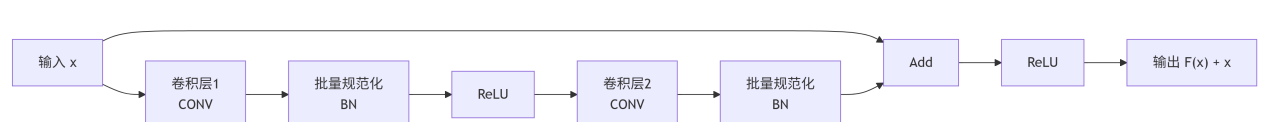
\includegraphics{images/image-0007.png}
\caption{ResNet 残差块结构}
\end{figure}

注意：F(x) + x~是逐元素相加（Element-wise Addition），意味着~F(x)~的输出必须与~x~的维度完全相同。这要求残差块内的最后一层卷积必须将通道数调整到与~x~一致。

ResNet通过堆叠上述残差块构建了不同深度的网络。

\hypertarget{ux4e09ux6b8bux5deeux7f51ux7edcux4e3aux4f55ux5982ux6b64ux6709ux6548}{%
\subsection{三、残差网络为何如此有效？}\label{ux4e09ux6b8bux5deeux7f51ux7edcux4e3aux4f55ux5982ux6b64ux6709ux6548}}

\begin{enumerate}
\def\labelenumi{\arabic{enumi}.}
\item
  解决梯度消失问题：~跳跃连接提供了一条``高速公路''，使得梯度可以从深层几乎无损耗地、直接地反向传播到浅层。这使得超深度网络的训练成为可能。
\item
  简化学习目标：~学习残差~F(x) = H(x) - x~通常比学习完整的映射~H(x)~更容易。特别是，当``恒等映射''已经是最优或接近最优时，将残差~F(x)~推近0比用一堆非线性层去拟合一个恒等映射要容易得多。
\item
  隐式的模型集成：~有理论认为，ResNet的行为类似于一个众多浅层网络的集成。由于跳跃连接的存在，数据可以沿不同深度的路径流动，使得网络同时具有浅层和深层的特性。
\end{enumerate}

\hypertarget{ux56dbux53d8ux4f53}{%
\subsection{四、变体}\label{ux56dbux53d8ux4f53}}

瓶颈结构（Bottleneck）：~为了在更深的网络（如ResNet-50/101/152）中减少计算量，每个残差块内采用了``瓶颈''设计：1x1卷积（降维） -\textgreater{} 3x3卷积 -\textgreater{} 1x1卷积（升维）。这大大减少了3x3卷积的计算开销。

\hypertarget{ux4e94ux73b0ux4ee3ux5927ux6a21ux578bux4e2dux6b8bux5deeux7684ux5e94ux7528}{%
\subsection{五、现代大模型中残差的应用}\label{ux4e94ux73b0ux4ee3ux5927ux6a21ux578bux4e2dux6b8bux5deeux7684ux5e94ux7528}}

现代大模型中，不是用一个从输入直接连到输出的残差一般在每个块或层中，都会加一个残差结构，以让梯度和信息顺畅流过该块或层，使信息流动更灵活，如 Transformer 架构里的多处 Add。

\hypertarget{ux53c2ux8003ux6587ux732e-12}{%
\subsection{参考文献}\label{ux53c2ux8003ux6587ux732e-12}}

\begin{itemize}
\tightlist
\item
  He, K., Zhang, X., Ren, S., \& Sun, J. (2016). \href{https://arxiv.org/abs/1512.03385}{Deep Residual Learning for Image Recognition}. CVPR 2016.
\end{itemize}

\clearpage

\hypertarget{densenet}{%
\section{DenseNet}\label{densenet}}

在ResNet中，我们看到了跳跃连接（x + F(x)）的巨大威力。DenseNet的作者提出了一个更激进的想法：为了最大化网络中各层之间的信息流动，能否让每一层都直接连接到它后面的所有层？

在这种连接模式下，每一层都从所有 preceding layers（前面的层）中接收``集体知识''作为输入，并将其自身的特征图传递给所有 subsequent layers（后面的层）。

\hypertarget{ux4e00ux6838ux5fc3ux7ec4ux4ef6ux5bc6ux96c6ux5757dense-blockux4e0eux8fc7ux6e21ux5c42transition-layer}{%
\subsection{一、核心组件：密集块（Dense Block）与过渡层（Transition Layer）}\label{ux4e00ux6838ux5fc3ux7ec4ux4ef6ux5bc6ux96c6ux5757dense-blockux4e0eux8fc7ux6e21ux5c42transition-layer}}

DenseNet的结构由两种核心模块交替组成。

\begin{enumerate}
\def\labelenumi{\arabic{enumi}.}
\tightlist
\item
  密集块（Dense Block）
\end{enumerate}

密集块是DenseNet的核心构建单元。在一个密集块内部，每一层都直接与块内的所有后续层相连。

数学表达：设第~l~层的输出为~x\_l，则第~l~层的输入是前面所有层输出的拼接（Concatenation）：x\_l = H\_l({[}x\_0, x\_1, \ldots, x\_\{l-1\}{]})
其中~{[} \ldots{} {]}~表示在通道维度（Channel Dimension）~上进行拼接，H\_l(·)~代表一个复合函数（如BN-ReLU-Conv）。

结构剖析：

复合函数~H\_l：~通常是一个标准的序列，包括批量规范化（BN）、ReLU激活函数~和~3x3卷积（Conv）。这个3x3卷积通常只产生很少的特征图（例如~k=32~个），这个数字~k~被称为增长率（Growth Rate）。

拼接操作：~每一层都会将其输出的~k~个特征图添加到整个块的``集体知识''中。因此，越靠后的层，其输入通道数会越多（因为它拼接了前面所有层的输出）。

局部连接：~密集连接只发生在密集块内部。不同密集块之间不直接连接。

\begin{enumerate}
\def\labelenumi{\arabic{enumi}.}
\setcounter{enumi}{1}
\tightlist
\item
  过渡层（Transition Layer）
\end{enumerate}

由于密集块内的拼接操作会使特征图的通道数快速增长（例如，一个包含10层、增长率k=32的块，最后一层的输入通道数可能高达~3 + 10*32 = 323），为了控制模型的复杂度和计算量，需要在密集块之间插入过渡层。

作用：~压缩特征图的尺寸和通道数，进行降维。

结构：~通常包含三个部分：

批量规范化（BN）

1x1卷积：~在DenseNet-C中引入，用于降低通道数。通常会将通道数减少一个比例（例如减少到原来的一半），这个比例是一个超参数。

2x2平均池化（Average Pooling）：~步幅为2，用于将特征图的高和宽减半，实现空间尺寸上的降采样。

\hypertarget{ux4e8cux6574ux4f53ux7f51ux7edcux67b6ux6784}{%
\subsection{二、整体网络架构}\label{ux4e8cux6574ux4f53ux7f51ux7edcux67b6ux6784}}

一个完整的DenseNet的结构例如：7\emph{7步长为2的初始卷积------最大池化------密集层------过渡层（1}1卷积+2*2平均池化）------密集层------过渡层------密集层------过渡层------密集层------全局平均池化------分类器

\hypertarget{ux4e09densenetux7684ux4f18ux52bfux4e0eux6311ux6218}{%
\subsection{三、DenseNet的优势与挑战}\label{ux4e09densenetux7684ux4f18ux52bfux4e0eux6311ux6218}}

优势：

\begin{enumerate}
\def\labelenumi{\arabic{enumi}.}
\item
  强大的抗过拟合能力：~参数效率极高，参数量远少于同等性能的ResNet或VGG，因此在数据量不是特别巨大的情况下表现优异。
\item
  极大地改善了梯度流：~密集的连接使得梯度能够直接传播到早期层，网络非常容易训练。
\item
  鼓励特征重用：~每一层都可以直接利用网络中最底层的原始特征和所有中间层的复合特征，模型非常高效。
\item
  自带正则化效果：~其结构本身就有抑制过拟合的效果。
\end{enumerate}

挑战与缺点：

\begin{enumerate}
\def\labelenumi{\arabic{enumi}.}
\item
  高内存消耗：~这是DenseNet最显著的缺点。由于需要保存所有中间特征图用于拼接，在训练过程中对GPU内存的消耗非常大。有许多研究致力于优化其内存效率。
\item
  潜在的计算开销：~大量的拼接操作也可能带来计算上的开销。
\item
  并非越深越好：~由于通道数的爆炸式增长，DenseNet的深度受到一定限制（通常最多几百层），不像ResNet可以轻松做到上千层。
\end{enumerate}

\hypertarget{ux56dbux901aux9053ux6570ux7206ux70b8ux95eeux9898}{%
\subsection{四、通道数``爆炸''问题}\label{ux56dbux901aux9053ux6570ux7206ux70b8ux95eeux9898}}

假设我们有一个DenseNet的密集块（Dense Block），并定义以下参数：

输入通道数：~假设进入第一个密集块的输入特征图有~C0 = 64~个通道。

增长率（Growth Rate）k：~这是DenseNet最重要的超参数之一。它定义了每个卷积层会产生多少新的特征图。假设~k = 32。这意味着每一层~H\_l（BN-ReLU-Conv）都会输出~32~个通道。

复合函数：~每一层都执行~H\_l:~BN → ReLU → 3×3 Conv~(输出~k~个通道)。

第0层（输入层）：输入到密集块的特征图：{[}通道数 = C0 = 64{]}

第1层：对这个~64~通道的输入进行~H\_1~操作（3x3卷积），并产生~k = 32~个新的特征图。

当前总特征图数：~64 (原有的) + 32 (新增的) = 96~个通道。

第2层：对这~96~个通道的输入进行~H\_2~操作，产生~32~个新的特征图。

当前总特征图数：~96 + 32 = 128~个通道。

第3层：~产生~32~个新特征图。

当前总特征图数：~128 + 32 = 160~个通道。

以此类推\ldots 第~l~层：输入通道数：~C0 + k × (l - 1)

对于一个包含~L~层的密集块，其最终输出的总通道数为：C\_\{output\} = C0 + k * L

虽然从数学上看是线性增长，但在深度学习实践中，这种增长带来的后果是``爆炸式''的

内存占用爆炸：若网络有~L~层，则第~l~层的输出特征图需被后续所有层复用，主流深度学习框架（如PyTorch、TensorFlow）在实现拼接操作（concat）时，会为每次拼接开辟独立的内存空间存储拼接结果，意味着它需在内存中保存~L−l+1~次。因此，全网络总内存消耗近似为O(L2)（平方级复杂度），而传统网络如ResNet仅为~O(L)（线性复杂度）。反向传播需依赖前向计算的中间特征图计算梯度。DenseNet因密集连接，需存储所有中间特征图，保存这些中间特征图用于反向传播会消耗巨大的GPU内存，成为训练DenseNet的主要瓶颈。

计算量增长：~尽管每一层只产生~k=32~个通道，但计算这些输出所需的卷积操作（Conv2D）的输入通道数却在不断变大，计算开销也随之增加。

DenseNet的解决方案：

\begin{enumerate}
\def\labelenumi{\arabic{enumi}.}
\item
  过渡层（Transition Layer）。1x1 卷积：~在DenseNet-C中引入，用于压缩通道数。例如，如果上一个密集块输出~C~个通道，1x1卷积会将其减少到~θC~个通道，其中~θ~是压缩因子（通常~θ=0.5）。这直接解决了通道数过多的问题。2x2 平均池化：将特征图的高和宽减半，进一步降低计算量。
\item
  更多优化
\end{enumerate}

（1）内存高效实现\hspace{0pt}

共享缓存机制：预分配一块固定缓存，供所有拼接层复用，避免重复开辟内存，将显存占用从~O(L2)~降至~O(L)。

梯度重构技术：反向传播时动态重建中间特征，减少存储需求（详见论文~Memory-Efficient Implementation of DenseNets）。

（2）结构压缩技术\hspace{0pt}

Bottleneck层（DenseNet-B）：在3×3卷积前添加1×1卷积压缩通道，降低计算量。

Transition层压缩（DenseNet-C）：通过压缩因子~θ（如0.5）减少特征图通道数。

DenseNet-BC：结合Bottleneck与Transition压缩，综合优化内存与计算效率。

（3）替代架构设计\hspace{0pt}

VoVNet（One-Shot Aggregation）：仅在模块最后一层聚合前面所有层特征，保留多尺度特征的同时，将MAC降至与ResNet相当。

通道剪枝与MFM（Max-Feature-Map）：对中间层特征进行通道选择，减少拼接时的通道数。

\hypertarget{ux53c2ux8003ux6587ux732e-13}{%
\subsection{参考文献}\label{ux53c2ux8003ux6587ux732e-13}}

\begin{itemize}
\tightlist
\item
  Huang, G., Liu, Z., van der Maaten, L., \& Weinberger, K. Q. (2017). \href{https://arxiv.org/abs/1608.06993}{Densely Connected Convolutional Networks}. CVPR 2017.
\end{itemize}

\clearpage

\hypertarget{ux57faux4e8eux5377ux79efux795eux7ecfux7f51ux7edcux7684ux76eeux6807ux68c0ux6d4bux7b97ux6cd5}{%
\section{基于卷积神经网络的目标检测算法}\label{ux57faux4e8eux5377ux79efux795eux7ecfux7f51ux7edcux7684ux76eeux6807ux68c0ux6d4bux7b97ux6cd5}}

卷积神经网络（CNN）及其变体具有很强的图像处理能力，无法直接做图像物体检测。这是因为图像中的物体数量是不确定的，如果逐个物体检测输出定位、分类，输出维度就会和物体数量有关，从而输出层维度不固定，而卷积神经网络的输出层维度是固定的。因而，诞生了许多基于卷积神经网络的目标检测算法。

\hypertarget{ux4e00ux6ed1ux52a8ux7a97ux53e3ux6cd5}{%
\subsection{一、滑动窗口法}\label{ux4e00ux6ed1ux52a8ux7a97ux53e3ux6cd5}}

设置不同大小和长宽比的窗口，从图像左上角开始，以一定的步长（Stride）滑动窗口，截取图像块。将截取下来的每一个小图像块resize到固定大小（如224*224），送入一个训练好的CNN分类器，判断这个小窗口里是``猫''、``狗''还是``背景''。

这种方法的缺点在于，一张图可能生成成千上万个子窗口，每个窗口都要过一遍CNN，计算大量冗余（相邻窗口像素高度重叠）。而且，它没有解决维度问题，而是通过多次运行来规避，本质是把检测问题强行拆解成了无数个单图分类问题。

\hypertarget{ux4e8cfaster-r-cnnux4e24ux9636ux6bb5ux7b97ux6cd5}{%
\subsection{二、Faster R-CNN：两阶段算法}\label{ux4e8cfaster-r-cnnux4e24ux9636ux6bb5ux7b97ux6cd5}}

在滑动窗口法中，重叠的像素被反复计算。Faster R-CNN让整张图只过一次CNN骨干网络（如ResNet50），得到一张特征图（Feature Map）。后续所有的操作（RPN 和分类）都在这张高维特征图上进行，极大地节省了算力。

\begin{enumerate}
\def\labelenumi{\arabic{enumi}.}
\tightlist
\item
  第一阶段：区域提议网络（Region Proposal Network, RPN）
\end{enumerate}

RPN 的目的是解决``框在哪里''的问题，它是一个全卷积网络。

输入：CNN 提取的特征图（例如大小为H\emph{W}C）。

锚框机制（Anchors）：为了处理不同大小和长宽比的物体，RPN在特征图的每一个像素点（对应原图的一个区域）上，预设k个不同尺度和比例的参考框（Anchors），通常k=9（3种尺度*3种长宽比）。

CNN卷积操作：使用一个3\emph{3的滑动窗口在特征图上卷积，随后连接两个1}1的卷积层（相当于全连接）：

（1）分类层（cls layer）：输出2k个分数（每个Anchor是前景/背景的概率）。

（2）回归层（reg layer）：输出4k个坐标偏移量（对Anchor的x, y, w, h进行微调）。

输出：筛选出分数较高的Anchor，经过非极大值抑制（NMS）后，得到一系列候选区域（Region of Interest, RoI）。

\begin{enumerate}
\def\labelenumi{\arabic{enumi}.}
\setcounter{enumi}{1}
\tightlist
\item
  第二阶段：RoI Pooling与精调
\end{enumerate}

这一步解决``特征维度统一''的问题。第一阶段生成的 RoI 大小各不相同（有的框大，有的框小），但后续的全连接层需要固定长度的输入。

RoI Pooling：将特征图上对应不同大小RoI的区域，强行通过池化操作（如最大池化）划分成固定大小（例如7*7）。

最终输出：将这个固定特征块展平，送入全连接层进行具体的类别分类（N+1类，含背景）和边框再次精修。

\hypertarget{ux4e09yoloyou-only-look-onceux4e00ux9636ux6bb5ux7b97ux6cd5}{%
\subsection{三、YOLO（You Only Look Once）：一阶段算法}\label{ux4e09yoloyou-only-look-onceux4e00ux9636ux6bb5ux7b97ux6cd5}}

YOLO算法将物体检测看作一个回归问题（Regression Problem）。彻底抛弃了``先提议、后分类''的流程，直接从图像像素映射到边界框坐标和类别概率。

\begin{enumerate}
\def\labelenumi{\arabic{enumi}.}
\tightlist
\item
  输入
\end{enumerate}

YOLO将输入图像划分为S*S个网格，通过网格划分解决输出维度不固定。如果一个物体的中心点落在这个网格中，那么这个网格就负责检测这个物体。即使图中有100个物体，甚至没有物体，YOLO的输出大小永远是固定的。

每个网格负责预测中心在该网格内的物体类别（训练阶段，物体中心在这格，期望输出就是在这格打上该物体的x,y,w,h,类别等标签，从而在测试阶段会呈现这样的``分工''），对于每个网格负责的物体会预测B个（YOLO v1一般取2个）可能的边界框（Bounding Box）。

\begin{enumerate}
\def\labelenumi{\arabic{enumi}.}
\setcounter{enumi}{1}
\tightlist
\item
  输出
\end{enumerate}

数据是一个S\emph{S}（5*B+Class）维的张量，分为三部分：

第一部分是每个框的中心横纵坐标x,y及框的大小w,h，数据个数S\emph{S}4*B。

第二部分是每个框的置信度Confidence，训练时期望输出=Pr*IOU，Pr在框内有物体时取1否则取0，训练时IOU=（预测框∩实际框的面积）/（预测框U实际框的面积），测试时输出本质上是对训练时期望输出的拟合。

第三部分是每个网格预测属于各类别的概率，共有Class个类别，数据个数S\emph{S}Class。

\begin{enumerate}
\def\labelenumi{\arabic{enumi}.}
\setcounter{enumi}{2}
\tightlist
\item
  损失函数
\end{enumerate}

YOLO的损失函数是它能训练成功的关键，它由定位误差、置信度误差和分类误差三部分加权求和而成。

（1）定位损失：x,y用均方损失，h,w则是对sqrt(h),sqrt(w)用均方损失，避免大目标的误差主导损失函数，这是因为同样的像素偏差（例如预测宽了5个像素），对于大框来说无伤大雅，但对于小框来说是巨大的错误。

（2）置信度损失：用均方损失，有物体中心的网格乘以较大的系数（如5），没有物体中心的网格乘以较小的系数（如0.5），这是因为物体检测置信度比背景更重要。

（3）分类损失：v1用均方损失，v2以后用交叉熵损失。

\hypertarget{ux53c2ux8003ux6587ux732e-14}{%
\subsection{参考文献}\label{ux53c2ux8003ux6587ux732e-14}}

\begin{itemize}
\tightlist
\item
  Redmon, J., Divvala, S., Girshick, R., \& Farhadi, A. (2016). \href{https://arxiv.org/abs/1506.02640}{You Only Look Once: Unified, Real-Time Object Detection}. CVPR 2016.
\item
  Redmon, J., \& Farhadi, A. (2017). \href{https://arxiv.org/abs/1612.08242}{YOLO9000: Better, Faster, Stronger}. CVPR 2017.
\item
  Redmon, J., \& Farhadi, A. (2018). \href{https://arxiv.org/abs/1804.02767}{YOLOv3: An Incremental Improvement}. arXiv:1804.02767.
\end{itemize}

\clearpage


% 循环神经网络
\hypertarget{ux5faaux73afux795eux7ecfux7f51ux7edc}{%
\chapter{循环神经网络}\label{ux5faaux73afux795eux7ecfux7f51ux7edc}}

\hypertarget{ux81eaux56deux5f52ux6a21ux578b}{%
\section{自回归模型}\label{ux81eaux56deux5f52ux6a21ux578b}}

\hypertarget{ux4e00ux6838ux5fc3ux601dux60f3}{%
\subsection{一、核心思想}\label{ux4e00ux6838ux5fc3ux601dux60f3}}

一个序列中当前时刻的值，可以由其过去若干个时刻的值的线性组合加上一个随机扰动（误差）来解释和预测。如基于这个上下文来预测最可能出现的``下一个''词。

一个~p阶~的自回归模型，记为~AR(p)，其公式定义为：

\[
X_t = c + \phi_1 X_{t-1} + \phi_2 X_{t-2} + \cdots + \phi_p X_{t-p} + \epsilon_t
\]

公式解读：

\begin{itemize}
\tightlist
\item
  \(X_t\)：当前时刻 \(t\) 的变量值（我们想要预测的值）。
\item
  \(c\)：常数项（截距）。
\item
  \(\phi_1, \phi_2, \ldots, \phi_p\)：自回归系数。这些是模型需要学习的参数，代表了过去每个时刻的值对当前值的影响程度和方向。
\item
  \(X_{t-1}, X_{t-2}, \ldots, X_{t-p}\)：过去 \(p\) 个时刻的历史值。
\item
  \(\epsilon_t\)：时刻 \(t\) 的随机误差项（白噪声）。它代表了模型无法用历史数据解释的随机波动，通常假设其均值为 0，方差恒定。
\end{itemize}

阶数 p决定了模型回看多远的过去。p 的选择至关重要，太小可能欠拟合，太大可能过拟合。

平稳性要求：序列的均值、方差和协方差不随时间推移而发生显著变化。如果不平稳，通常需要通过差分等方法将其转换为平稳序列（这就引出了ARIMA模型中的``I''）。

\hypertarget{ux4e8cux5e94ux7528}{%
\subsection{二、应用}\label{ux4e8cux5e94ux7528}}

\begin{enumerate}
\def\labelenumi{\arabic{enumi}.}
\tightlist
\item
  LLM：将生成问题看作一个序列生成问题（词序列、token序列）。模型定义了一个条件概率分布：\(P(x_t | x_{<t})\)。即，给定所有已经生成的词 \(x_1, x_2, ..., x_{t-1}\)，计算下一个词 \(x_t\) 的概率分布。从该分布中采样（或取最可能）得到下一个词 \(x_t\)。将新生成的词 \(x_t\) 加入上下文，重复步骤，直到生成序列结束符或达到最大长度。
\end{enumerate}

实现技术：~通过掩码机制（Causal Masking）~实现。在Transformer中，确保在计算第t个位置的注意力时，只能``看到''第1到第t-1个位置的信息，无法看到``未来''的信息，从而严格保证了自回归的特性。

\begin{enumerate}
\def\labelenumi{\arabic{enumi}.}
\setcounter{enumi}{1}
\tightlist
\item
  计算机视觉：也可以用``给定之前所有生成的概率，预测下一个像素的概率分布''的方法生成非常清晰、高质量的图像，但缺点是非常慢，因为必须逐个像素顺序生成，无法并行。
\end{enumerate}

\hypertarget{ux53c2ux8003ux6587ux732e-15}{%
\subsection{参考文献}\label{ux53c2ux8003ux6587ux732e-15}}

\begin{itemize}
\tightlist
\item
  Aston Zhang, Zachary C. Lipton, Mu Li, Alexander J. Smola. (2023). \href{https://zh.d2l.ai/}{《动手学深度学习》}. Cambridge University Press.
\end{itemize}

\clearpage

\hypertarget{ux5faaux73afux795eux7ecfux7f51ux7edcrnn}{%
\section{循环神经网络（RNN）}\label{ux5faaux73afux795eux7ecfux7f51ux7edcrnn}}

\hypertarget{ux4e00ux6838ux5fc3ux601dux60f3-1}{%
\subsection{一、核心思想}\label{ux4e00ux6838ux5fc3ux601dux60f3-1}}

RNN的核心思想是为网络引入``记忆''或``状态''的概念，使其能够保留之前输入的信息，并用于影响当前输出的计算。

前馈神经网络（如CNN、MLP）假设所有输入（和输出）之间是相互独立的。处理一个输入样本时，不会考虑它之前或之后的样本，没有``上下文''的概念。每次前向计算时，输入的样本的数据量是恒定的。对于基于此设计的 \(n\) 元语法模型（\(n\) 给定），要预测下一个词 \(x_t\)，它只会回头看紧挨着的前 \(n-1\) 个词 \(x_{t-1},\ldots,x_{t-n+1}\)，但如果 \(n\) 变得很大，模型需要记录所有可能的 \(n\) 个词组合的概率。假设词表有10万个词，一个 \(n=4\) 的模型就需要存储 \(100{,}000^4\) 个概率值，这是一个天文数字，在计算和存储上都是不可能的。

为了解决 \(n\) 增大带来的参数爆炸问题，我们引入一个隐变量模型。这个模型不再直接依赖于所有过去的历史词，而是依赖于一个总结了过去所有历史信息的中间变量，称为隐状态（hidden state）。新的模型化为：

\[
P(x_t \mid x_{t-1},\ldots,x_1) \approx P(x_t \mid h_{t-1})
\]

这个隐状态 \(h_{t-1}\) 是一个向量，它封装了从序列开始到 \(t-1\) 时刻的所有有用信息。它的维度是固定的（比如256维），不会因为序列变长而改变大小。这就巧妙地避免了参数随历史长度指数增长。基于此设计的循环神经网络（RNN）专门设计用于处理序列数据，即输入（或输出）是一个接一个的、相互关联的数据点。例如时间序列数据（股票价格、天气数据、传感器读数）、自然语言（句子、段落，本质上是词的序列）、音频/视频（按时间顺序排列的帧或采样点）。

\hypertarget{ux4e8cux6570ux5b66ux8868ux8fbe}{%
\subsection{二、数学表达}\label{ux4e8cux6570ux5b66ux8868ux8fbe}}

\begin{enumerate}
\def\labelenumi{\arabic{enumi}.}
\tightlist
\item
  新的隐藏层：
\end{enumerate}

\[
h_t=f(x_t,h_{t-1})=\phi(W_{xh}x_t+W_{hh}h_{t-1}+b_h)
\]

\(W_{xh}x_t\)：这是一个线性变换，将当前输入 \(x_t\)（一个代表词的数字向量）投影到隐藏空间。

\(W_{hh}h_{t-1}\)：这是另一个线性变换，将过去的隐状态（记忆）也投影到隐藏空间。权重矩阵 \(W_{hh}\) 是RNN最关键的部分，它决定了过去的记忆如何影响当前状态。

\(b_h\)：偏置项。

\(\phi\)：一个非线性激活函数（如 \(\tanh\) 或ReLU）。\(\tanh\) 函数可以将值压缩到 \((-1,1)\) 之间，有助于稳定网络的输出。

\begin{enumerate}
\def\labelenumi{\arabic{enumi}.}
\setcounter{enumi}{1}
\tightlist
\item
  生成输出：新的隐藏状态 \(h_t\) 通常可以直接用作输出，或者再通过一个输出层进行计算。当前时刻的最终输出为：
\end{enumerate}

\[
o_t=W_{ho}h_t+b_o
\]

\begin{enumerate}
\def\labelenumi{\arabic{enumi}.}
\setcounter{enumi}{2}
\tightlist
\item
  参数更新：通过时间反向传播（BPTT）
\end{enumerate}

（1）将网络按时间步展开成一个深度的前馈网络

想象RNN在处理一个长度为5的序列 \([x_1,x_2,x_3,x_4,x_5]\)。前向传播时，RNN逐步计算：

\[
h_1=f(x_1,h_0)\to h_2=f(x_2,h_1)\to h_3=f(x_3,h_2)\to h_4=f(x_4,h_3)\to h_5=f(x_5,h_4)
\]

BPTT的视角：它把这个过程看成是一个5层的特殊DNN：

第1层：输入是 \([x_1,h_0]\)，输出是 \(h_1\)

第2层：输入是 \([x_2,h_1]\)，输出是 \(h_2\)

\ldots{}

这个``深度网络''的特殊之处在于：所有``层''都共享同一组参数 \((W_{xh}, W_{hh}, b_h)\)。第 \(t\) 层的输入不仅包括原始输入 \(x_t\)，还包括前一层的输出 \(h_{t-1}\)。

（2）反向传播

我们以一个简单的 RNN 为例，其隐状态更新公式为：

\[
h_t = \tanh(W_{xh}x_t + W_{hh}h_{t-1} + b_h)
\]

最终输出和损失为：

\[
o_t = W_{hq}h_t + b_q
\]

\[
L = \sum_{t=1}^{T} L_t = \sum_{t=1}^{T} \mathrm{Loss}(o_t, y_t)
\]

A. 计算最终输出层参数的梯度（\(W_{hq}, b_q\)）

这部分最简单，因为 \(o_t\) 只依赖于 \(h_t\)，梯度不跨时间步传播，可以按时间步独立计算再求和。

\[
\frac{\partial L}{\partial W_{hq}}
= \sum_{t=1}^{T} \frac{\partial L_t}{\partial o_t}\frac{\partial o_t}{\partial W_{hq}}
= \sum_{t=1}^{T}(o_t - y_t) \cdot h_t^T
\]

\[
\frac{\partial L}{\partial b_q}
= \sum_{t=1}^{T} \frac{\partial L_t}{\partial o_t}\frac{\partial o_t}{\partial b_q}
= \sum_{t=1}^{T}(o_t - y_t)
\]

B. 计算循环层参数的梯度（\(W_{xh}, W_{hh}, b_h\)）

总损失 \(L\) 依赖于 \(h_t\)，而 \(h_t\) 又依赖于 \(h_{t-1}\) 和参数，这种依赖关系一直传递到序列开始。因此，梯度计算涉及跨时间步的链式法则。

我们定义一个关键变量：损失对 \(t\) 时刻隐状态的梯度 \(\delta_t\)。

\[
\delta_t = \frac{\partial L}{\partial h_t}
\]

\begin{enumerate}
\def\labelenumi{\arabic{enumi}.}
\tightlist
\item
  从最后一个时间步 \(T\) 开始初始化：
\end{enumerate}

\(\delta_T\) 由两部分构成：来自当前输出的损失和来自未来的损失。但在许多简单情况下，如果 \(h_T\) 只影响 \(o_T\)，则：

\[
\delta_T = \frac{\partial L_T}{\partial h_T}
= \frac{\partial L_T}{\partial o_T}\frac{\partial o_T}{\partial h_T}
= (o_T - y_T) W_{hq}^T
\]

\begin{enumerate}
\def\labelenumi{\arabic{enumi}.}
\setcounter{enumi}{1}
\tightlist
\item
  对于 \(t = T-1, T-2, \ldots, 1\)，梯度递归地反向传播：
\end{enumerate}

\[
\delta_t = \frac{\partial L_t}{\partial h_t} + \frac{\partial h_{t+1}}{\partial h_t}\delta_{t+1}
\]

其中，第一项来自当前输出，第二项来自未来时间步。

\hypertarget{ux4e09ux4f20ux7edfrnnux5b58ux5728ux7684ux95eeux9898grulstmux7684ux63d0ux51faux80ccux666f}{%
\subsection{三、传统RNN存在的问题（GRU、LSTM的提出背景）}\label{ux4e09ux4f20ux7edfrnnux5b58ux5728ux7684ux95eeux9898grulstmux7684ux63d0ux51faux80ccux666f}}

\begin{enumerate}
\def\labelenumi{\arabic{enumi}.}
\tightlist
\item
  梯度消失与梯度爆炸
\end{enumerate}

这是RNN最著名的问题。在反向传播时，梯度需要沿着时间步一路相乘回去。

如果 \(W_{hh}\)（隐藏状态权重矩阵）的特征值小于1，连续相乘会导致梯度变得极小，以至于较早时间步的参数无法得到有效更新，难以修正其在序列早期犯下的错误（网络``忘记''了远处的事情）。而如果想强行让模型记住早期信息，就需要早期参数产生一个在反向传播中不衰减的巨大梯度，这要么在数学上很难自然发生，要么会引发另一个问题（引发梯度爆炸，影响其他参数训练）导致训练失败。

反之，如果特征值大于1，梯度会指数级增长（梯度爆炸），导致训练不稳定，网络参数更新剧烈，无法收敛。

\begin{enumerate}
\def\labelenumi{\arabic{enumi}.}
\setcounter{enumi}{1}
\tightlist
\item
  长程依赖问题
\end{enumerate}

梯度消失的直接后果就是模型难以学习到序列中远距离的依赖关系。例如，在句子``The clouds which have been covering the sky all day are finally starting to \_\_\_''中，要预测最后一个词``clear''或``rain''，模型需要记住很久之前的主语``clouds''。

传统RNN的困境：由于梯度消失，网络很难将第一个时间步的信息（误差）一路传递到最后一个时间步。为了学会记住这个信息，网络必须给第一个时间步分配一个巨大的梯度，这在实际训练中很难实现。

所需的机制：需要一个``记忆单元''，能够像计算机硬盘一样，稳定地存储关键信息很长一段时间，而不受后续操作（梯度计算）的干扰。

\begin{enumerate}
\def\labelenumi{\arabic{enumi}.}
\setcounter{enumi}{2}
\tightlist
\item
  难以满足忽略无关信息需求
\end{enumerate}

例子：在分析网页情感时，HTML标签（如 \texttt{\textless{}div\textgreater{}}、\texttt{\textless{}br\textgreater{}}）与情感无关，是噪声。

传统RNN的困境：传统RNN会无差别地处理每一个输入，这些无关词元也会更新隐状态，污染后续有用的信息。

所需的机制：需要一个``遗忘''或``跳过''机制，能够主动选择哪些信息是重要的需要流入，哪些是不重要的需要被忽略。

\begin{enumerate}
\def\labelenumi{\arabic{enumi}.}
\setcounter{enumi}{3}
\tightlist
\item
  难以满足重置内部状态需求
\end{enumerate}

例子：序列的不同部分之间存在明显边界或主题转换，比如书的新章节开始，或市场行情从熊市转为牛市。

传统RNN的困境：传统RNN的隐状态会不断地累积历史信息。当场景突然切换时，旧章节或旧行情的信息会持续影响新章节或新行情的学习，造成干扰。

所需的机制：需要一个``重置''机制，能够在检测到逻辑中断时，有选择地清除过去的、不再相关的记忆，从而更好地初始化新场景的学习。

\hypertarget{ux53c2ux8003ux6587ux732e-16}{%
\subsection{参考文献}\label{ux53c2ux8003ux6587ux732e-16}}

\begin{itemize}
\tightlist
\item
  Aston Zhang, Zachary C. Lipton, Mu Li, Alexander J. Smola. (2023). \href{https://zh.d2l.ai/}{《动手学深度学习》}. Cambridge University Press.
\end{itemize}

\clearpage

\hypertarget{ux7f16ux7801ux5668-ux89e3ux7801ux5668ux67b6ux6784}{%
\section{编码器-解码器架构}\label{ux7f16ux7801ux5668-ux89e3ux7801ux5668ux67b6ux6784}}

编码器-解码器（Encoder-Decoder）架构的目标是将一个输入序列（例如一句英文句子）(x₁, x₂, \ldots, x\_T)~转换成一个输出序列（例如一句中文句子）(y₁, y₂, \ldots, y\_T')。两个序列的长度可以不同。

编码器：读取并``理解''整个输入序列，将其压缩成一个固定维度的上下文向量（Context Vector）~c，这个向量旨在包含输入序列的完整语义信息。

解码器：以该上下文向量~c~作为初始``记忆''和``指令''，开始逐步生成输出序列。

\hypertarget{ux4e00ux7f16ux7801ux5668encoder}{%
\subsection{一、编码器（Encoder）}\label{ux4e00ux7f16ux7801ux5668encoder}}

编码器是一个RNN（可以是普通RNN、LSTM或GRU）。它逐个处理输入序列中的每个词元。

对于每一个时间步~t~(从 1 到~T)，编码器执行以下计算：
h\_t\^{}\{enc\} = f\_\{enc\}(x\_t, h\_\{t-1\}\^{}\{enc\})

h\_t\^{}\{enc\}： 编码器在时间步~t~的隐状态。

f\_\{enc\}： 编码器RNN的函数（例如，LSTM单元的计算过程）。它包含可学习的参数~W\_\{xh\}\textsuperscript{\{enc\},~W\_\{hh\}}\{enc\},~b\_h\^{}\{enc\}~等以及激活函数。

x\_t： 时间步~t~的输入词嵌入向量。

h\_\{t-1\}\^{}\{enc\}： 上一个时间步的隐状态。初始隐状态~h\_0\^{}\{enc\}~通常初始化为全零向量。

上下文向量的生成：
在处理完整个输入序列后，编码器最后一个时间步的隐状态~h\_T\^{}\{enc\}~被用作上下文向量~c。
c = h\_T\^{}\{enc\}

这个向量~c~承载了编码器从整个输入序列中读取并整合的所有信息。它将被用作解码器的初始状态。

更高级的架构中，c~可以是一个池化后的结果，或者是注意力机制的加权组合，但最经典的形式就是~h\_T\^{}\{enc)。

\hypertarget{ux4e8cux89e3ux7801ux5668decoder}{%
\subsection{二、解码器（Decoder）}\label{ux4e8cux89e3ux7801ux5668decoder}}

解码器是另一个RNN，其目标是生成输出序列。它的初始状态由编码器提供的上下文向量初始化。

数学表达：解码器在每一个时间步~t'~(从 1 到~T') 的计算分为两部分：

\begin{enumerate}
\def\labelenumi{\alph{enumi})}
\tightlist
\item
  计算当前隐状态：
  s\_\{t'\} = f\_\{dec\}(y\_\{t'-1\}, s\_\{t'-1\})
\end{enumerate}

s\_\{t'\}： 解码器在时间步~t'~的隐状态。

f\_\{dec\}： 解码器RNN的函数，参数~W\_\{xh\}\textsuperscript{\{dec\},~W\_\{hh\}}\{dec\},~b\_h\^{}\{dec\}~等。

s\_\{t'-1\}： 解码器上一个时间步的隐状态。关键点：初始状态~s\_0~被设置为上下文向量~c。
s\_0 = c

y\_\{t'-1\}：~解码器在上一个时间步~生成~的输出。在训练和推理时，这个输入的策略不同（详见后面的`` teacher forcing''）。

\begin{enumerate}
\def\labelenumi{\alph{enumi})}
\setcounter{enumi}{1}
\tightlist
\item
  计算当前输出：
  解码器的隐状态~s\_\{t'\}~被送入一个输出层（通常是全连接层 + Softmax），以预测当前时间步的输出词元概率分布。
  o\_\{t'\} = g(s\_\{t'\}) = \text{softmax}(W\_\{out\} s\_\{t'\} + b\_\{out\})
  P(y\_\{t'\} \textbar{} y\_\{\textless t'\}, c) = o\_\{t'\}
\end{enumerate}

o\_\{t'\}： 一个概率分布向量，其维度与输出词表大小相同。每个值代表了对应词元是当前时间步~t'~输出的概率。一般而言，每个词由

W\_\{out\},~b\_\{out\}： 输出层的权重和偏置参数。

解码器生成序列的过程是一个自回归（Autoregressive）过程：

初始状态~s\_0 = c，初始输入通常是一个特殊的~token。

计算~s\_1~和~o\_1，从~o\_1~中采样或取argmax得到第一个词~y₁。

将~y₁~作为下一个时间步的输入，计算~s\_2~和~o\_2，得到~y₂。

重复此过程，直到生成一个特殊的~token，表示序列生成结束。

\hypertarget{ux4e09ux603bux7ed3ux4e0eux5b8cux6574ux7684ux6570ux5b66ux6d41ux7a0b}{%
\subsection{三、总结与完整的数学流程}\label{ux4e09ux603bux7ed3ux4e0eux5b8cux6574ux7684ux6570ux5b66ux6d41ux7a0b}}

将一个输入序列~X = (x₁, x₂, \ldots, x\_T)~翻译为输出序列~Y = (y₁, y₂, \ldots, y\_\{T'\})：

\begin{enumerate}
\def\labelenumi{\arabic{enumi}.}
\item
  编码器阶段：
  h\_t\^{}\{enc\} = f\_\{enc\}(x\_t, h\_\{t-1\}\^{}\{enc\}), \quad \text{for } t = 1, \ldots, T
  c = h\_T\^{}\{enc\}
\item
  解码器阶段：
  s\_0 = c
  s\_\{t'\} = f\_\{dec\}(y\_\{t'-1\}, s\_\{t'-1\}), \quad \text{for } t' = 1, \ldots, T'
  P(y\_\{t'\} \textbar{} y\_\{\textless t'\}, c) = g(s\_\{t'\}) = \text{softmax}(W\_\{out\} s\_\{t'\} + b\_\{out\})
\item
  训练目标和损失：
  最大化输出序列的条件对数似然：
  要log P(Y\textbar X) 最大，也就是sum(log P(y\_\{t'\} \textbar{} y\_\{\textless t'\})最大；而-log P(y\_\{t'\} \textbar{} y\_\{\textless t'\})就是交叉熵损失，让模型趋向于真实one-hot分布
\item
  一个重要技巧：Teacher Forcing
\end{enumerate}

在训练时，解码器每一步的输入~y\_\{t'-1\}~有一个重要选择：

不使用Teacher Forcing： 使用解码器自己上一步预测的结果作为输入。错误会累积，训练可能不稳定。

使用Teacher Forcing： 无论解码器上一步预测的是什么，都强制使用真实标签（Ground Truth）~中的上一个词~y\_\{t'-1\}\^{}\{true\}~作为输入。

s\_\{t'\} = f\_\{dec\}(y\_\{t'-1\}\^{}\{true\}, s\_\{t'-1\})

这大大加速了训练的收敛，因为它在每一步都为解码器提供了正确的上下文。然而，这可能导致训练和推理时的不匹配（Exposure Bias），因为推理时没有真实标签可用。通常采用一种课程学习策略，在训练后期逐渐减少Teacher Forcing的使用。

推理时，则没有真实标签可用，只能使用解码器自己上一步的预测结果作为当前步的输入。

\hypertarget{ux53c2ux8003ux6587ux732e-17}{%
\subsection{参考文献}\label{ux53c2ux8003ux6587ux732e-17}}

\begin{itemize}
\tightlist
\item
  Aston Zhang, Zachary C. Lipton, Mu Li, Alexander J. Smola. (2023). \href{https://zh.d2l.ai/}{《动手学深度学习》}. Cambridge University Press.
\end{itemize}

\clearpage

\hypertarget{ux95e8ux63a7ux8bb0ux5fc6ux5355ux5143gru}{%
\section{门控记忆单元（GRU）}\label{ux95e8ux63a7ux8bb0ux5fc6ux5355ux5143gru}}

\hypertarget{ux4e00ux57faux672cux539fux7406}{%
\subsection{一、基本原理}\label{ux4e00ux57faux672cux539fux7406}}

\begin{enumerate}
\def\labelenumi{\arabic{enumi}.}
\tightlist
\item
  重置门~R\_t：控制``可能还想记住''的过去状态的数量。它决定了有多少过去的信息需要被``忘记''（如网页中html码等无用信息，我们不希望其参与候选状态计算），以便与新输入结合形成新的候选状态。
\end{enumerate}

重置门有助于捕获序列中的短期依赖关系。它通过控制有多少过去信息参与新候选状态的计算，来影响当前时刻的即时反应。这对于理解紧邻词元之间的关系（短期模式）非常有效。

\begin{enumerate}
\def\labelenumi{\arabic{enumi}.}
\setcounter{enumi}{1}
\tightlist
\item
  更新门~Z\_t：控制新状态中旧状态和候选状态的比例。它决定了有多少过去的信息会被直接保留到新的状态中（如一些必须原样保留的信息）。
\end{enumerate}

更新门~有助于捕获序列中的长期依赖关系。它通过控制信息传递的路径，让网络能够直接复制过去的状态。如果模型学到让更新门在很长一段时间内都保持接近1，那么很久以前的信息就可以几乎无损地传递到未来，从而完美地解决了梯度消失问题，擅长捕捉长期模式。

接下来，GRU 不是直接计算新的隐状态，而是先计算一个候选隐状态（Candidate Hidden State）\(\tilde{H}_t\)。这个候选状态表示在当前输入和经过筛选的过去信息共同作用下可能形成的新状态。

重置门 \(R_t\) 在这里起到关键作用：它通过与前一状态 \(H_{t-1}\) 进行按元素乘法（Hadamard 积）来``重置''或``过滤''过去的信息。

\begin{itemize}
\tightlist
\item
  如果重置门 \(R_t\) 的某个元素接近 1，则表示允许对应的过去信息通过，公式退化为类似传统 RNN 的更新方式 \(\tanh(X_t W_{xh} + H_{t-1}W_{hh} + b_h)\)。
\item
  如果重置门 \(R_t\) 的某个元素接近 0，则会``屏蔽''或``忘记''对应的过去信息。此时，候选状态仅由当前输入 \(X_t\) 决定（类似于一个简单的 MLP），这有助于忽略无关信息。
\end{itemize}

公式为：

\[
\tilde{H}_t = \tanh(X_t W_{xh} + (R_t \odot H_{t-1})W_{hh} + b_h)
\]

其中，\(\odot\) 表示 Hadamard 积（按元素相乘），\(\tanh\) 激活函数确保候选状态的值在 \((-1, 1)\) 之间。

最后，新的隐状态 \(H_t\) 是旧状态 \(H_{t-1}\) 和候选状态 \(\tilde{H}_t\) 之间的凸组合，这个组合的比例由更新门 \(Z_t\) 控制。

\begin{itemize}
\tightlist
\item
  如果更新门 \(Z_t\) 的某个元素接近 1，则新状态会大量保留旧状态的信息，几乎忽略掉候选状态（即当前输入的影响很小）。这使得网络能够跳过不重要的时间步，从而有效地将很久以前的信息传递下去，解决长期依赖问题。
\item
  如果更新门 \(Z_t\) 的某个元素接近 0，则新状态会更倾向于采用候选状态，即更多地关注当前输入。
\end{itemize}

这种机制使得 GRU 可以灵活地选择是``记住''长期信息还是``关注''短期输入。

公式为：

\[
H_t = Z_t \odot H_{t-1} + (1 - Z_t) \odot \tilde{H}_t
\]

形象理解：

GRU~像一个高效的现代工作站：

重置门：在思考新方案(\textasciitilde h\_t)前，先清空一下白板上不相关的内容。

更新门：决定最终的白板(h\_t)上，要擦掉多少旧内容，又要把新方案写上去多少。

两个思考的问题：

\begin{enumerate}
\def\labelenumi{\arabic{enumi}.}
\tightlist
\item
  为什么这里要单独用门，而不是直接调控权重？
\end{enumerate}

因为门有一个重要的特性：``按元素乘''

在传统矩阵乘法中，调一个权重必然涉及到与之相乘的所有元素，因而想通过这一方式保留或抹去特定位置的信息是很难的。门中的元素则和神经元一一对应。

\begin{enumerate}
\def\labelenumi{\arabic{enumi}.}
\setcounter{enumi}{1}
\tightlist
\item
  为什么两个门不能相互替代？
\end{enumerate}

如果只有重置门，没有更新门，候选隐状态计算函数很难直接拟合恒等变换y=x，无法保证信息原样传递；如果只有更新门，没有重置门，个别元素上的无关信息就会影响候选状态（因为前面讲过的原因，不能把对应权重直接设为0）。

\hypertarget{ux4e8cux91cdux7f6eux95e8ux4e0eux66f4ux65b0ux95e8ux7684ux8ba1ux7b97}{%
\subsection{二、重置门与更新门的计算}\label{ux4e8cux91cdux7f6eux95e8ux4e0eux66f4ux65b0ux95e8ux7684ux8ba1ux7b97}}

对于给定的时间步 \(t\)：

\[
R_t = \sigma(X_t W_{xr} + H_{t-1}W_{hr} + b_r)
\]

\[
Z_t = \sigma(X_t W_{xz} + H_{t-1}W_{hz} + b_z)
\]

其中：

\begin{itemize}
\tightlist
\item
  \(\sigma\) 是 sigmoid 激活函数。
\item
  \(W_{xr}, W_{xz}\) 是与输入 \(X_t\) 相乘的权重矩阵。
\item
  \(W_{hr}, W_{hz}\) 是与前一隐状态 \(H_{t-1}\) 相乘的权重矩阵。
\item
  \(b_r, b_z\) 是偏置参数。
\end{itemize}

那么，重置门和更新门为什么要由当前时间步的输入 X\_t 和前一个时间步的隐状态 H\_\{t-1\} 通过一个全连接层，再经过 sigmoid 激活函数计算得到？

\begin{enumerate}
\def\labelenumi{\arabic{enumi}.}
\tightlist
\item
  目的：门控需要成为``情境感知''的决策器
  这两个门在每个时刻都要做两个关键决策：
\end{enumerate}

重置门：为了处理好眼前这个新输入，我该忘掉多少刚才还记得的背景信息？

更新门：我是应该 mostly 记住旧的，还是应该~mostly 相信新的？

这些决策绝不能是死板的规则，必须根据当前具体遇到什么词、处在什么上下文环境中来灵活决定。

举个例子（情感分析）：
句子是：``This movie is not good at all, it is actually terribly boring.''

当模型读到~``not''~这个词时：

重置门应该意识到：下一个词~``good''~的意思要反转了！必须弱化/重置掉之前~``is''~带来的正面预感，准备好接收一个被否定后的信息。

更新门应该意识到：``not''~是个超级重要的信号！必须牢牢记住这个状态，把它强有力地传递下去，影响后面所有词的判断。

如果门控是固定的或者只由当前词决定，它就无法根据整个句子的上下文（由过去的隐藏状态编码）来做出如此精细和关键的决策。

所以，门控的决策必须基于两大信息源：

当前观测 (X\_t)：我现在看到了什么词？

历史上下文 (H\_\{t-1\})：我之前读到过什么，正处于什么样的理解背景下？

只有把这两者结合起来，门控才能做出最明智的、懂场景的（Context-Aware）~决策。

\begin{enumerate}
\def\labelenumi{\arabic{enumi}.}
\setcounter{enumi}{1}
\tightlist
\item
  结构：让模型自己学会权衡
  将当前输入和过去状态分别乘以权重再加起来，这个结构（称为``仿射变换''）是在让模型自己通过训练数据学习：在面对什么样的情况下，应该更相信当前输入；在什么样的情况下，应该更依赖历史记忆。
\end{enumerate}

对于能颠覆语义的词（如~``not'',~``but''），模型会学会让当前输入的权重很大，从而让当前词主导门的开关。

对于不重要的词（如~``the'',~``a''），模型会学会让历史状态的权重占主导，从而命令门控：``忽略它，保持原状！''

这种设计给了模型极大的灵活性。

\begin{enumerate}
\def\labelenumi{\arabic{enumi}.}
\setcounter{enumi}{2}
\tightlist
\item
  激活函数：Sigmoid------完美的``比例调节器''
  Sigmoid函数是一个神奇的``压缩器''，它能把任何大小的数字都变成一个介于0和1之间的值。
\end{enumerate}

完美的解释性：输出是0到1之间，可以天然地理解为~``开度的百分比''。比如：0是``全关''，1是``全开''，0.7是``开七成''。

可训练性：这个函数是光滑的，这对于使用反向传播算法来训练模型至关重要，误差可以顺利地通过它传回去调整权重。

清晰的决策：虽然它在极端情况下会饱和（导致梯度消失），但在门控这里这反而是个优点。它允许门的输出无限接近0或1，从而实现非常坚决的``开''或``关''的决策，形成稳定的记忆流。

\hypertarget{ux4e09ux603bux7ed3}{%
\subsection{三、总结}\label{ux4e09ux603bux7ed3}}

通过重置门和更新门的协同工作，GRU能够动态地、有选择地管理记忆，从而在各种序列建模任务中取得优异的效果。

\hypertarget{ux53c2ux8003ux6587ux732e-18}{%
\subsection{参考文献}\label{ux53c2ux8003ux6587ux732e-18}}

\begin{itemize}
\tightlist
\item
  Aston Zhang, Zachary C. Lipton, Mu Li, Alexander J. Smola. (2023). \href{https://zh.d2l.ai/}{《动手学深度学习》}. Cambridge University Press.
\item
  Cho, K., van Merrienboer, B., Gulcehre, C., et al.~(2014). \href{https://arxiv.org/abs/1406.1078}{Learning Phrase Representations using RNN Encoder-Decoder for Statistical Machine Translation}. EMNLP 2014.
\end{itemize}

\clearpage

\hypertarget{ux957fux77edux671fux8bb0ux5fc6ux7f51ux7edclstm}{%
\section{长短期记忆网络（LSTM）}\label{ux957fux77edux671fux8bb0ux5fc6ux7f51ux7edclstm}}

\hypertarget{ux4e00ux53ccux72b6ux6001ux67b6ux6784}{%
\subsection{一、双状态架构}\label{ux4e00ux53ccux72b6ux6001ux67b6ux6784}}

记忆元（\(C_t\)）：内部的、私有的长期记忆。它像一条隐藏的传送带，主要负责长期信息的保留和传递。

隐状态（\(h_t\)）：对外的、暴露的短期记忆/输出。它是当前时间步的输出，也是下一个时间步的输入的一部分。

\hypertarget{ux4e8cux6838ux5fc3ux6b65ux9aa4ux548cux95e8ux63a7}{%
\subsection{二、核心步骤和门控}\label{ux4e8cux6838ux5fc3ux6b65ux9aa4ux548cux95e8ux63a7}}

第一步：计算候选记忆元：

\[
\tilde{C}_t = \tanh(W_C [h_{t-1}, x_t] + b_C)
\]

第二步：更新记忆元：

\[
C_t = f_t \odot C_{t-1} + i_t \odot \tilde{C}_t
\]

这里 \(f_t\) 是忘记门，与上一个记忆元状态 \(C_{t-1}\) 逐点相乘。接近 \(0\) 的值意味着``忘记这个信息''，接近 \(1\) 的值意味着``完整保留这个信息''；\(i_t\) 是输入门，决定候选神经元各点的信息被写入记忆元的程度。二者组合的效果有点类似于 GRU 中的更新门，但并不限制二者的和必须为 \(1\)，事实上缓解了梯度消失（和为 \(1\) 意味着大量零点几的权重）。

第三步：计算当前隐状态（输出）：

\[
h_t = o_t \odot \tanh(C_t)
\]

\(o_t\) 为输出门，是连接记忆元和隐状态的桥梁，决定从 \(C_t\) 中读出什么到 \(h_t\)。

形象表达：

LSTM~像一个有严格文件管理流程的办公室：

忘记门：决定档案室（\(C_t\)）里哪些旧文件要碎掉。

输入门：决定今天收到的新文件（\(\tilde{C}_t\)）有多少要归档。

输出门：决定从档案室拿出哪些文件给来访者看（\(h_t\)）。

思考的问题：

\begin{enumerate}
\def\labelenumi{\arabic{enumi}.}
\tightlist
\item
  LSTM中没有类似GRU中重置门的结构，那 HTML 标签之类的无关信息就会影响候选记忆元的计算，对此LSTM是怎么避免它带来的问题的？
\end{enumerate}

因为当遇到 \texttt{\textless{}div\textgreater{}}、\texttt{\textless{}/p\textgreater{}} 这类 HTML 标签时，训练好的 LSTM 会让输入门对应受标签影响的几个位置的 \(i_t \approx 0\)，同时，忘记门 \(f_t\) 可以保持接近 \(1\)，完整保留之前的记忆。而且即便这里处理不好，还有输出门作为``保险''。

\begin{enumerate}
\def\labelenumi{\arabic{enumi}.}
\setcounter{enumi}{1}
\tightlist
\item
  为什么能有效解决传统RNN的梯度消失？
\end{enumerate}

LSTM的记忆元更新公式：

\[
C_t = f_t \odot C_{t-1} + i_t \odot \tilde{C}_t
\]

这个公式可以看作是两个部分的加权和：一部分是过去的记忆 \(C_{t-1}\)，另一部分是当前候选记忆 \(\tilde{C}_t\)。

在反向传播时，我们需要计算 \(C_t\) 对 \(C_{t-1}\) 的梯度。根据求导法则，这个梯度是：

\[
\frac{\partial C_t}{\partial C_{t-1}} = f_t
\]

这里忽略掉候选记忆元对 \(C_{t-1}\) 的依赖，因为通常我们只考虑直接依赖，而且候选记忆元本身也是通过 \(C_{t-1}\) 计算的，但这里看主要路径。

注意，这个梯度中有一个重要的部分：忘记门 \(f_t\)。而且，这个梯度是加在 \(C_{t-1}\) 上的，而不是通过一个压缩性的非线性函数（如 \(\tanh\)）的导数。

在传统RNN中，\(h_t = \tanh(W [h_{t-1}, x_t] + b)\)，梯度会连续乘以 \(\tanh\) 的导数（该导数小于 \(1\)），导致梯度指数级缩小。而在LSTM中，记忆元的梯度直接是 \(f_t\)，而且这个 \(f_t\) 是通过 sigmoid 函数得到的，范围在 \(0\) 到 \(1\) 之间。但是，关键点在于：这个梯度不是连续乘以一个小于 \(1\) 的数，而是乘以 \(f_t\)。如果 \(f_t\) 接近 \(1\)，那么梯度就可以几乎无损地传递到上一个时间步。

因此，记忆元的梯度在反向传播时，可以沿着时间步保持一个相对稳定的值，而不会指数级消失。这就像是一条``高速公路''，梯度可以沿着这条公路直接流动，从而缓解了梯度消失。

\hypertarget{ux4e09ux4e09ux4e2aux95e8ux7684ux8ba1ux7b97}{%
\subsection{三、三个门的计算}\label{ux4e09ux4e09ux4e2aux95e8ux7684ux8ba1ux7b97}}

忘记门：

\[
f_t = \sigma(W_f [h_{t-1}, x_t] + b_f)
\]

输入门：

\[
i_t = \sigma(W_i [h_{t-1}, x_t] + b_i)
\]

输出门：

\[
o_t = \sigma(W_o [h_{t-1}, x_t] + b_o)
\]

其中 \(\sigma\) 是 sigmoid 函数，保证三者值在 \((0,1)\)。

\hypertarget{ux56dbux603bux7ed3}{%
\subsection{四、总结}\label{ux56dbux603bux7ed3}}

整体上，相对于GRU而言，LSTM参数更多，计算更复杂，通常在更复杂的数据集上表现更优，数据量不大时则相对GRU无显著优势。

\hypertarget{ux53c2ux8003ux6587ux732e-19}{%
\subsection{参考文献}\label{ux53c2ux8003ux6587ux732e-19}}

\begin{itemize}
\tightlist
\item
  Aston Zhang, Zachary C. Lipton, Mu Li, Alexander J. Smola. (2023). \href{https://zh.d2l.ai/}{《动手学深度学习》}. Cambridge University Press.
\item
  Hochreiter, S., \& Schmidhuber, J. (1997). \href{https://doi.org/10.1162/neco.1997.9.8.1735}{Long Short-Term Memory}. Neural Computation.
\end{itemize}

\clearpage

\hypertarget{ux6df1ux5ea6ux5faaux73afux795eux7ecfux7f51ux7edc}{%
\section{深度循环神经网络}\label{ux6df1ux5ea6ux5faaux73afux795eux7ecfux7f51ux7edc}}

到目前为止，我们只讨论了具有一个单向隐藏层的循环神经网络。其中，隐变量和观测值与具体的函数形式的交互方式是相当随意的。 只要交互类型建模具有足够的灵活性，这就不是一个大问题。然而，对一个单层来说，这可能具有相当的挑战性。之前在线性模型中，我们通过添加更多的层来解决这个问题。 而在循环神经网络中，我们首先需要确定如何添加更多的层，以及在哪里添加额外的非线性，因此这个问题有点棘手。

事实上，我们可以将多层循环神经网络堆叠在一起，通过对几个简单层的组合，产生了一个灵活的机制。特别是，数据可能与不同层的堆叠有关。例如，我们可能希望保持有关金融市场状况（熊市或牛市）的宏观数据可用，而微观数据只记录较短期的时间动态。

下图描述了一个具有 \(L\) 个隐藏层的深度循环神经网络，每个隐状态都连续地传递到当前层的下一个时间步和下一层的当前时间步。

\begin{figure}[htbp]
\centering
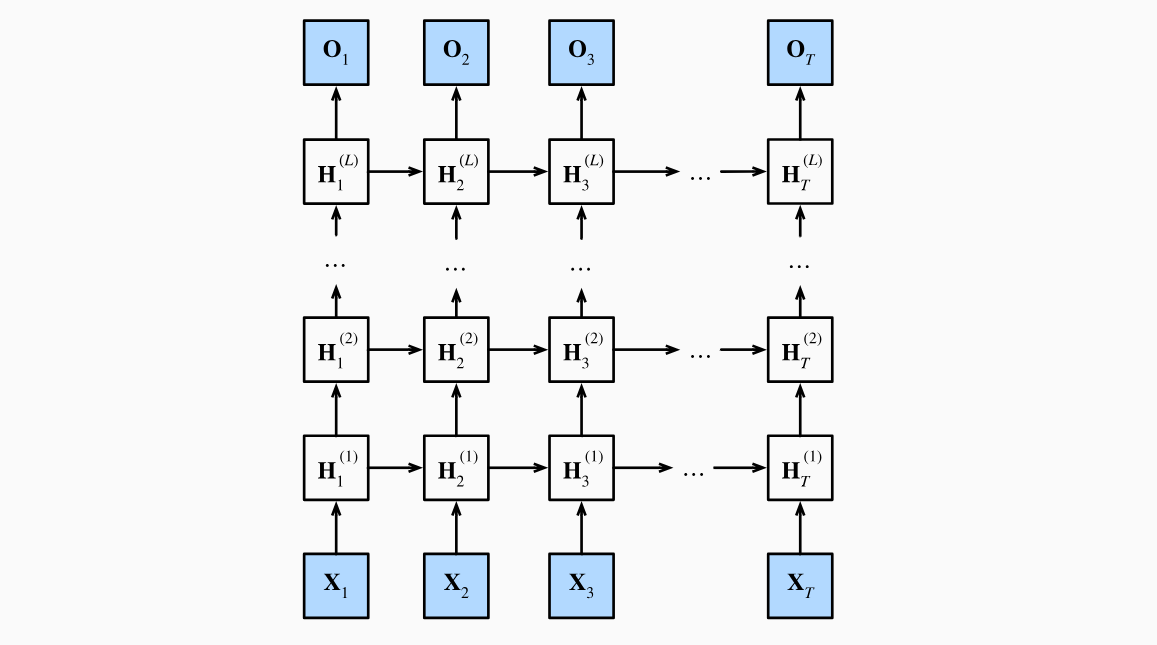
\includegraphics{images/image-0008.png}
\caption{深度循环神经网络结构}
\end{figure}

我们可以将深度架构中的函数依赖关系形式化，这个架构由 \(L\) 个隐藏层构成。后续的讨论主要集中在经典的循环神经网络模型上，但这些讨论也适用于其他序列模型。

假设在时间步 \(t\) 有一个小批量的输入数据 \(X_t \in \mathbb{R}^{n \times d}\)（样本数为 \(n\)，每个样本中的输入数为 \(d\)）。同时，将第 \(l\) 个隐藏层（\(l = 1, \ldots, L\)）的隐状态设为 \(H_t^{(l)} \in \mathbb{R}^{n \times h}\)（隐藏单元数为 \(h\)），输出层变量设为 \(O_t \in \mathbb{R}^{n \times q}\)（输出数为 \(q\)）。设置 \(H_t^{(0)} = X_t\)，第 \(l\) 个隐藏层的隐状态使用激活函数 \(\phi_l\)，则：

\[
H_t^{(l)} = \phi_l(H_t^{(l-1)}W_{xh}^{(l)} + H_{t-1}^{(l)}W_{hh}^{(l)} + b_h^{(l)})
\]

其中，权重 \(W_{xh}^{(l)} \in \mathbb{R}^{h \times h}\)、\(W_{hh}^{(l)} \in \mathbb{R}^{h \times h}\) 和偏置 \(b_h^{(l)} \in \mathbb{R}^{1 \times h}\) 都是第 \(l\) 个隐藏层的模型参数。

最后，输出层的计算仅基于第 \(L\) 个隐藏层最终的隐状态：

\[
O_t = H_t^{(L)}W_{hq} + b_q
\]

其中，权重 \(W_{hq} \in \mathbb{R}^{h \times q}\) 和偏置 \(b_q \in \mathbb{R}^{1 \times q}\) 都是输出层的模型参数。

与多层感知机一样，隐藏层数目 \(L\) 和隐藏单元数目 \(h\) 都是超参数，可以由我们调整。另外，用门控循环单元或长短期记忆网络的隐状态来代替上式中的隐状态进行计算，可以很容易地得到深度门控循环神经网络或深度长短期记忆神经网络。

\hypertarget{ux53c2ux8003ux6587ux732e-20}{%
\subsection{参考文献}\label{ux53c2ux8003ux6587ux732e-20}}

\begin{itemize}
\tightlist
\item
  Aston Zhang, Zachary C. Lipton, Mu Li, Alexander J. Smola. (2023). \href{https://zh.d2l.ai/}{《动手学深度学习》}. Cambridge University Press.
\end{itemize}

\clearpage

\hypertarget{ux53ccux5411ux5faaux73afux795eux7ecfux7f51ux7edc}{%
\section{双向循环神经网络}\label{ux53ccux5411ux5faaux73afux795eux7ecfux7f51ux7edc}}

\hypertarget{ux4e00ux9690ux9a6cux5c14ux53efux592bux6a21ux578bux4e2dux7684ux52a8ux6001ux89c4ux5212}{%
\subsection{一、隐马尔可夫模型中的动态规划}\label{ux4e00ux9690ux9a6cux5c14ux53efux592bux6a21ux578bux4e2dux7684ux52a8ux6001ux89c4ux5212}}

如果我们想用概率图模型来解决这个问题，可以设计一个隐变量模型：在任意时间步 \(t\)，假设存在某个隐变量 \(h_t\)，通过概率 \(P(x_t \mid h_t)\) 控制我们观测到的 \(x_t\)。此外，任何 \(h_t \to h_{t+1}\) 转移都由一些状态转移概率 \(P(h_{t+1} \mid h_t)\) 给出。这个概率图模型就是一个隐马尔可夫模型（hidden Markov model，HMM），如下图所示。

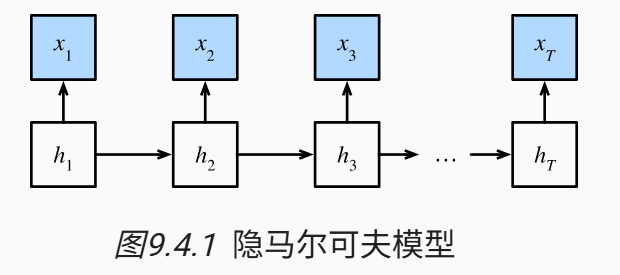
\includegraphics{images/image-0009.png}

因此，对于有 \(T\) 个观测值的序列，我们在观测状态和隐状态上具有以下联合概率分布：

\[
P(x_1, \ldots, x_T, h_1, \ldots, h_T)
= \prod_{t=1}^{T} P(h_t \mid h_{t-1})P(x_t \mid h_t), \quad P(h_1 \mid h_0) = P(h_1)
\]

现在，假设我们观测到所有的 \(x_i\)，除了 \(x_j\)，并且我们的目标是计算 \(P(x_j \mid x_{-j})\)，其中 \(x_{-j} = (x_1, \ldots, x_{j-1}, x_{j+1}, \ldots, x_T)\)。由于 \(P(x_j \mid x_{-j})\) 中没有隐变量，因此我们考虑对 \(h_1, \ldots, h_T\) 选择构成的所有可能的组合进行求和。如果任何 \(h_i\) 可以接受 \(k\) 个不同的值（有限的状态数），这意味着我们需要对 \(k^T\) 个项求和，这个任务显然难于登天。幸运的是，有个巧妙的解决方案：动态规划（dynamic programming）。

\begin{enumerate}
\def\labelenumi{\arabic{enumi}.}
\tightlist
\item
  前向递归（``对上次递推''）
\end{enumerate}

为了理解动态规划的工作方式，我们考虑对隐变量 \(h_1, \ldots, h_T\) 的依次求和。根据上面的联合分布可得：

\[
\begin{aligned}
P(x_1, \ldots, x_T)
&= \sum_{h_1,\ldots,h_T} P(x_1, \ldots, x_T, h_1, \ldots, h_T) \\
&= \sum_{h_1,\ldots,h_T} \prod_{t=1}^{T} P(h_t \mid h_{t-1})P(x_t \mid h_t) \\
&= \sum_{h_2,\ldots,h_T}\left[\sum_{h_1}P(h_1)P(x_1 \mid h_1)P(h_2 \mid h_1)\right]P(x_2 \mid h_2)\prod_{t=3}^{T}P(h_t \mid h_{t-1})P(x_t \mid h_t) \\
&= \sum_{h_3,\ldots,h_T}\left[\sum_{h_2}\pi_2(h_2)P(x_2 \mid h_2)P(h_3 \mid h_2)\right]P(x_3 \mid h_3)\prod_{t=4}^{T}P(h_t \mid h_{t-1})P(x_t \mid h_t) \\
&= \ldots \\
&= \sum_{h_T}\pi_T(h_T)P(x_T \mid h_T)
\end{aligned}
\]

其中，\(\pi_t(h_t)\) 表示所有得到 \((h_1, \ldots, h_{t-1}, h_t, x_1, \ldots, x_{t-1})\) 的路径概率之和。换句话说，它是在已观测 \(x_1, \ldots, x_{t-1}\) 后到达 \(t\) 时刻隐状态 \(h_t\) 的累计概率。因此，最后只需要对 \(h_T\) 求和即可。

通常，我们将前向递归（forward recursion）写为：

\[
\pi_{t+1}(h_{t+1}) = \sum_{h_t}\pi_t(h_t)P(x_t \mid h_t)P(h_{t+1} \mid h_t)
\]

递归被初始化为 \(\pi_1(h_1) = P(h_1)\)。符号简化后，也可以写成 \(\pi_{t+1} = f(\pi_t, x_t)\)，其中 \(f\) 是一些可学习的函数。这看起来就像我们在循环神经网络中讨论的隐变量模型中的更新方程。

\begin{enumerate}
\def\labelenumi{\arabic{enumi}.}
\setcounter{enumi}{1}
\tightlist
\item
  后向递归（``对下次递推''）
\end{enumerate}

这里我们设的 \(\rho_t(h_t)\) 是``在已经得到 \(h_t, x_t\) 条件下，最终得到 \((x_{t+1}, \ldots, x_T)\) 的概率''，是``给定状态下的预测概率''，包含了对经过的各种可能的 \(h_{t+1}, \ldots, h_T\) 路径概率的求和。

为了反向进行动态规划，可以从序列末尾逐步把未来路径的概率合并到 \(\rho\) 中：

\[
\begin{aligned}
P(x_1, \ldots, x_T)
&= \sum_{h_1,\ldots,h_T} P(x_1, \ldots, x_T, h_1, \ldots, h_T) \\
&= \sum_{h_1,\ldots,h_T}\prod_{t=1}^{T-1}P(h_t \mid h_{t-1})P(x_t \mid h_t)\cdot P(h_T \mid h_{T-1})P(x_T \mid h_T) \\
&= \sum_{h_1,\ldots,h_{T-1}}\prod_{t=1}^{T-1}P(h_t \mid h_{t-1})P(x_t \mid h_t)\cdot \left[\sum_{h_T}P(h_T \mid h_{T-1})P(x_T \mid h_T)\right] \\
&= \sum_{h_1,\ldots,h_{T-2}}\prod_{t=1}^{T-2}P(h_t \mid h_{t-1})P(x_t \mid h_t)\cdot \left[\sum_{h_{T-1}}P(h_{T-1} \mid h_{T-2})P(x_{T-1} \mid h_{T-1})\rho_{T-1}(h_{T-1})\right] \\
&= \ldots \\
&= \sum_{h_1}P(h_1)P(x_1 \mid h_1)\rho_1(h_1)
\end{aligned}
\]

因此，我们可以将后向递归（backward recursion）写为：

\[
\rho_{t-1}(h_{t-1}) = \sum_{h_t}P(h_t \mid h_{t-1})P(x_t \mid h_t)\rho_t(h_t)
\]

注：这里 \(\rho_1(h_1)\) 内部已经包含了对经过各种 \(h_2, \ldots, h_T\) 路径的求和。

为保证 \(t=T\) 时公式形式的一致性，初始化 \(\rho_T(h_T)=1\)。前向和后向递归都允许我们对 \(T\) 个隐变量在 \(O(kT)\)（线性而不是指数）时间内对 \((h_1,\ldots,h_T)\) 的所有值求和，这是使用图模型进行概率推理的巨大好处之一。它也是通用消息传递算法的一个非常特殊的例子。

\begin{enumerate}
\def\labelenumi{\arabic{enumi}.}
\setcounter{enumi}{2}
\tightlist
\item
  二者的结合
\end{enumerate}

如果我们只知道时间序列输出 \(x_1,\ldots,x_T\) 中除了 \(x_j\) 之外其他所有元素，但不知道隐状态 \(h_1,\ldots,h_T\)，这时如果逐个枚举每个 \(h_j\) 的全部可取的值（假设每个 \(h_j\) 的取值空间有 \(k\) 个值），其计算复杂度为 \(O(k^T)\)，显然行不通。

这里我们采用前向递归与后向递归结合的方法：

\[
P(x_j \mid x_{-j}) \propto \sum_{h_j}\pi_j(h_j)\rho_j(h_j)P(x_j \mid h_j)
\]

这里分母是得到除了 \(x_j\) 之外其他所有元素的概率，是和隐状态无关的常数。因为符号简化的需要，后向递归也可以写为 \(\rho_{t-1}=g(\rho_t,x_t)\)，其中 \(g\) 是一个可以学习的函数。同样，这看起来非常像一个更新方程，只是它不像我们在循环神经网络中看到的那样是前向运算，而是后向计算。事实上，知道未来数据何时可用对隐马尔可夫模型是有益的；信号处理学家将是否知道未来观测这种情况区分为内插和外推。

从计算复杂度的角度，无论是前向递归还是后向递归，对 \(T\) 个隐变量的情况对 \((h_1,\ldots,h_T)\) 的所有取值情况求和，递归计算过程的计算复杂度均为 \(O(kT)\)。上述公式相当于 \(x_j\) 以前取前向递归，以后取后向递归，计算复杂度仍然为 \(O(kT)\)。（注：这里的计算复杂度是执行计算时的，并不包括训练阶段训练概率值之类的）

\hypertarget{ux4e8cux53ccux5411ux5faaux73afux795eux7ecfux7f51ux7edc}{%
\subsection{二、双向循环神经网络}\label{ux4e8cux53ccux5411ux5faaux73afux795eux7ecfux7f51ux7edc}}

在序列学习中，我们以往假设的目标是：在给定观测的情况下（例如，在时间序列的上下文中或在语言模型的上下文中）， 对下一个输出进行建模。但实际上，对于文章挖空填空这样的任务，每个短语的``下文''传达了重要信息（如果有的话），而这些信息关乎到选择哪个词来填空， 所以无法利用这一点的序列模型将在相关任务上表现不佳。例如，如果要做好命名实体识别 （例如，识别``Green''指的是``格林先生''还是绿色）， 不同长度的上下文范围重要性是相同的。

对于任意时间步 \(t\)，给定一个小批量的输入数据 \(\mathbf{X}_t \in \mathbb{R}^{n \times d}\)（样本数 \(n\)，每个示例中的输入数 \(d\)），并且令隐藏层激活函数为 \(\phi\)。

在双向架构中，我们设该时间步的前向和反向隐状态分别为 \(\overrightarrow{\mathbf{H}}_t \in \mathbb{R}^{n \times h}\) 和 \(\overleftarrow{\mathbf{H}}_t \in \mathbb{R}^{n \times h}\)，其中 \(h\) 是隐藏单元的数目。前向和反向隐状态的更新如下：

\[
\begin{aligned}
\overrightarrow{\mathbf{H}}_t &= \phi(\mathbf{X}_t\mathbf{W}_{xh}^{(f)} + \overrightarrow{\mathbf{H}}_{t-1}\mathbf{W}_{hh}^{(f)} + \mathbf{b}_h^{(f)}), \\
\overleftarrow{\mathbf{H}}_t &= \phi(\mathbf{X}_t\mathbf{W}_{xh}^{(b)} + \overleftarrow{\mathbf{H}}_{t+1}\mathbf{W}_{hh}^{(b)} + \mathbf{b}_h^{(b)})
\end{aligned}
\]

其中，权重 \(\mathbf{W}_{xh}^{(f)} \in \mathbb{R}^{d \times h}\)、\(\mathbf{W}_{hh}^{(f)} \in \mathbb{R}^{h \times h}\)、\(\mathbf{W}_{xh}^{(b)} \in \mathbb{R}^{d \times h}\)、\(\mathbf{W}_{hh}^{(b)} \in \mathbb{R}^{h \times h}\) 和偏置 \(\mathbf{b}_h^{(f)} \in \mathbb{R}^{1 \times h}\)、\(\mathbf{b}_h^{(b)} \in \mathbb{R}^{1 \times h}\) 都是模型参数。

接下来，将前向隐状态 \(\overrightarrow{\mathbf{H}}_t\) 和反向隐状态 \(\overleftarrow{\mathbf{H}}_t\) 连接起来，获得需要送入输出层的隐状态 \(\mathbf{H}_t \in \mathbb{R}^{n \times 2h}\)。在具有多个隐藏层的深度双向循环神经网络中，该信息作为输入传递到下一个双向层。最后，输出层计算得到的输出为 \(\mathbf{O}_t \in \mathbb{R}^{n \times q}\)（\(q\) 是输出单元的数目）：

\[
\mathbf{O}_t = \mathbf{H}_t\mathbf{W}_{hq} + \mathbf{b}_q
\]

这里，权重矩阵 \(\mathbf{W}_{hq} \in \mathbb{R}^{2h \times q}\) 和偏置 \(\mathbf{b}_q \in \mathbb{R}^{1 \times q}\) 是输出层的模型参数。事实上，这两个方向可以拥有不同数量的隐藏单元。

双向循环神经网络的一个关键特性是：使用来自序列两端的信息来估计输出。也就是说，我们使用来自过去和未来的观测信息来预测当前的观测。但是在对下一个词元进行预测的情况中，这样的模型并不是我们所需的。因为在预测下一个词元时，我们终究无法知道下一个词元的下文是什么，所以将不会得到很好的精度。具体地说，在训练期间，我们能够利用过去和未来的数据来估计现在空缺的词；而在测试期间，我们只有过去的数据，因此精度将会很差。下面的实验将说明这一点。

另一个严重问题是，双向循环神经网络的计算速度非常慢。其主要原因是网络的前向传播需要在双向层中进行前向和后向递归，并且网络的反向传播还依赖于前向传播的结果。因此，梯度求解将有一个非常长的链。

双向层的使用在实践中非常少，并且仅仅应用于部分场合。例如，填充缺失的单词、词元注释（例如，用于命名实体识别），以及作为序列处理流水线中的一个步骤对序列进行编码（例如，用于机器翻译）。在相关后续章节中，将介绍如何使用双向循环神经网络编码文本序列。

\hypertarget{ux53c2ux8003ux6587ux732e-21}{%
\subsection{参考文献}\label{ux53c2ux8003ux6587ux732e-21}}

\begin{itemize}
\tightlist
\item
  Aston Zhang, Zachary C. Lipton, Mu Li, Alexander J. Smola. (2023). \href{https://zh.d2l.ai/}{《动手学深度学习》}. Cambridge University Press.
\item
  Schuster, M., \& Paliwal, K. K. (1997). \href{https://doi.org/10.1109/78.650093}{Bidirectional recurrent neural networks}. IEEE Transactions on Signal Processing.
\end{itemize}

\clearpage

\hypertarget{ux5e8fux5217ux5230ux5e8fux5217seq2sequx5b66ux4e60}{%
\section{序列到序列（Seq2Seq）学习}\label{ux5e8fux5217ux5230ux5e8fux5217seq2sequx5b66ux4e60}}

从技术上讲，编码器将长度可变的输入序列转换成形状固定的上下文变量 \(\mathbf{c}\)，并且将输入序列的信息在该上下文变量中进行编码。可以使用循环神经网络来设计编码器。

考虑由一个序列组成的样本（批量大小是 1）。假设输入序列是 \(x_1,\ldots,x_T\)，其中 \(x_t\) 是输入文本序列中的第 \(t\) 个词元。在时间步 \(t\)，循环神经网络将词元 \(x_t\) 的输入特征向量 \(\mathbf{x}_t\) 和 \(\mathbf{h}_{t-1}\)（即上一时间步的隐状态）转换为 \(\mathbf{h}_t\)（即当前步的隐状态）。使用一个函数 \(f\) 来描述循环神经网络的循环层所做的变换：

\[
\mathbf{h}_t = f(\mathbf{x}_t,\mathbf{h}_{t-1})
\]

总之，编码器通过选定的函数 \(q\)，将所有时间步的隐状态转换为上下文变量：

\[
\mathbf{c} = q(\mathbf{h}_1,\ldots,\mathbf{h}_T)
\]

正如上文提到的，编码器输出的上下文变量 \(\mathbf{c}\) 对整个输入序列 \(x_1,\ldots,x_T\) 进行编码。来自训练数据集的输出序列 \(y_1,y_2,\ldots,y_{T'}\)，对于每个时间步 \(t'\)（与输入序列或编码器的时间步 \(t\) 不同），解码器输出 \(y_{t'}\) 的概率取决于先前的输出子序列 \(y_1,\ldots,y_{t'-1}\) 和上下文变量 \(\mathbf{c}\)，即 \(P(y_{t'} \mid y_1,\ldots,y_{t'-1},\mathbf{c})\)。

为了在序列上模型化这种条件概率，我们可以使用另一个循环神经网络作为解码器。在输出序列上的任意时间步 \(t'\)，循环神经网络将来自上一时间步的输出 \(y_{t'-1}\) 和上下文变量 \(\mathbf{c}\) 作为其输入，然后在当前时间步将它们和上一隐状态 \(\mathbf{s}_{t'-1}\) 转换为隐状态 \(\mathbf{s}_{t'}\)。因此，可以使用函数 \(g\) 表示解码器的隐藏层的变换：

\[
\mathbf{s}_{t'} = g(y_{t'-1},\mathbf{c},\mathbf{s}_{t'-1})
\]

在获得解码器的隐状态之后，我们可以使用输出层和 softmax 操作来计算在时间步 \(t'\) 时输出 \(y_{t'}\) 的条件概率分布 \(P(y_{t'} \mid y_1,\ldots,y_{t'-1},\mathbf{c})\)。

在每个时间步，解码器预测了输出词元的概率分布。类似于语言模型，可以使用softmax来获得分布，并通过计算交叉熵损失函数来进行优化。另外，为了让不同长度的序列可以以相同形状的小批量加载。 特定的填充词元被添加到序列的末尾， 我们应该将填充词元的预测排除在损失函数的计算之外。用sequence\_mask函数可通过零值化屏蔽不相关的项， 以便后面任何不相关预测的计算都是与零的乘积，结果都等于零（交叉熵损失-sigma(pi*logqi),pi=0）。

\hypertarget{ux53c2ux8003ux6587ux732e-22}{%
\subsection{参考文献}\label{ux53c2ux8003ux6587ux732e-22}}

\begin{itemize}
\tightlist
\item
  Aston Zhang, Zachary C. Lipton, Mu Li, Alexander J. Smola. (2023). \href{https://zh.d2l.ai/}{《动手学深度学习》}. Cambridge University Press.
\end{itemize}

\clearpage


% 优化算法
\hypertarget{ux4f18ux5316ux7b97ux6cd5}{%
\chapter{优化算法}\label{ux4f18ux5316ux7b97ux6cd5}}

\hypertarget{ux968fux673aux68afux5ea6ux4e0bux964dsgd}{%
\section{随机梯度下降（SGD）}\label{ux968fux673aux68afux5ea6ux4e0bux964dsgd}}

随机梯度下降（SGD），即对于随机打乱顺序的样本，每次取一个或取一个批量（Batch）进行梯度下降。

\hypertarget{ux4e00ux5728ux8badux7ec3ux4e2dsgdux9762ux4e34ux7684ux95eeux9898}{%
\subsection{一、在训练中SGD面临的问题}\label{ux4e00ux5728ux8badux7ec3ux4e2dsgdux9762ux4e34ux7684ux95eeux9898}}

收敛速度问题：在特定地形（如狭长``峡谷''或鞍点）下收敛极其缓慢。

学习率选择问题：所有参数共享一个学习率，难以适应不同参数（特征）的梯度尺度。

Adam 优化器正是为了同时解决这两个问题，它结合了两种先进的优化思想：Momentum (动量法) 和 RMSProp。

\hypertarget{ux4e8csgdux5728ux5f3aux5316ux5faeux8c03ux4e2dux6548ux679cux53cdux800cux53efux80fdux4e0dux900aux4e8eadamw2025}{%
\subsection{二、SGD在强化微调中效果反而可能不逊于AdamW（2025）}\label{ux4e8csgdux5728ux5f3aux5316ux5faeux8c03ux4e2dux6548ux679cux53cdux800cux53efux80fdux4e0dux900aux4e8eadamw2025}}

论文《Reinforcement Learning Finetunes Small Subnetworks in Large Language Models》指出，在强化微调中，大部分参数事实上是不变的，强化微调具有内生稀疏性。本质上说，语义关联性已经在预训练中学习好了，强化微调主要是调整它们的概率分布，以强化正确的推理路径。因此局部优化曲面简单，不需要AdamW这种复杂系统。在AdamW中，由于自带动量和自适应机制，局部梯度很小也会更新，导致参数改动大，实际上很多是噪音；在SGD中，只有梯度显著的才会被调整，符合强化微调实际需求。

实验证明，用SGD进行全量微调，实际修改的参数可能比LoRA还少，效果却不逊于用AdamW进行全量微调。学习率需要取较大的值（1e-1左右）。

\hypertarget{ux53c2ux8003ux6587ux732e-23}{%
\subsection{参考文献}\label{ux53c2ux8003ux6587ux732e-23}}

\begin{itemize}
\tightlist
\item
  Robbins, H., \& Monro, S. (1951). \href{https://doi.org/10.1214/aoms/1177729586}{A Stochastic Approximation Method}. The Annals of Mathematical Statistics.
\item
  Bottou, L., Curtis, F. E., \& Nocedal, J. (2018). \href{https://epubs.siam.org/doi/10.1137/16M1080173}{Optimization Methods for Large-Scale Machine Learning}. SIAM Review.
\item
  Mukherjee, S., Yuan, L., Hakkani-Tur, D., \& Peng, H. (2025). \href{https://arxiv.org/abs/2505.11711}{Reinforcement Learning Finetunes Small Subnetworks in Large Language Models}. NeurIPS 2025.
\end{itemize}

\clearpage

\hypertarget{ux52a8ux91cfux6cd5momentum}{%
\section{动量法（Momentum）}\label{ux52a8ux91cfux6cd5momentum}}

\hypertarget{ux4e00momentum-ux89e3ux51b3ux4e86ux4ec0ux4e48ux95eeux9898}{%
\subsection{一、Momentum 解决了什么问题？}\label{ux4e00momentum-ux89e3ux51b3ux4e86ux4ec0ux4e48ux95eeux9898}}

Momentum主要解决了SGD在特定地形下的收敛速度和稳定性问题。

\begin{enumerate}
\def\labelenumi{\arabic{enumi}.}
\tightlist
\item
  狭窄``峡谷''地形的震荡
\end{enumerate}

描述： 想象一个损失函数的等高线图，它像一个狭长的山谷。在``山谷''的陡峭方向（两侧峭壁），梯度很大；但在``山谷''的平缓方向（通向谷底的最优解），梯度很小。

SGD的问题：SGD在陡峭方向上会因为梯度过大而来回震荡（Overshooting），这导致它在平缓方向上的前进速度非常缓慢。

\begin{enumerate}
\def\labelenumi{\arabic{enumi}.}
\setcounter{enumi}{1}
\tightlist
\item
  鞍点和平坦区域
\end{enumerate}

描述： 在高维空间中，局部最小值（Local Minima）其实较少，更常见的是鞍点。在鞍点处，所有方向的梯度都接近于零。

SGD的问题：当梯度趋于0时，SGD的更新步骤也会接近于零，导致优化器``卡住''，停止更新。

\hypertarget{ux4e8cmomentum-ux5982ux4f55ux89e3ux51b3ux95eeux9898}{%
\subsection{二、Momentum 如何解决问题？}\label{ux4e8cmomentum-ux5982ux4f55ux89e3ux51b3ux95eeux9898}}

Momentum引入了物理学中``动量''或``惯性''的概念。想象一个球从山上滚下：它不仅仅受当前位置的坡度影响，还携带着过去积累的速度（即``动量''）。

在陡峭方向，梯度 \(g_t\) 来回反向（\(+C, -C, +C, -C, \ldots\)）。当它们被累积到动量 \(m_t\) 中时，这些正负梯度会相互抵消，使得 \(m_t\) 在该方向上的分量减小，从而抑制了震荡。

在平缓方向，梯度 \(g_t\) 始终指向同一个方向（\(-c, -c, -c, \ldots\)）。动量 \(m_t\) 会持续累积这些同向的梯度，使得 \(m_t\) 在该方向上的分量增大，从而加速了前进。

当小球滚到一个鞍点时，虽然当前梯度 \(g_t\) 接近 \(0\)，但只要它携带着过去的动量（\(m_{t-1}>0\)），它就能凭借这股``惯性''``冲''过这个平坦区域，继续向最优解前进。

\hypertarget{ux4e09ux6570ux5b66ux8868ux8fbe}{%
\subsection{三、数学表达}\label{ux4e09ux6570ux5b66ux8868ux8fbe}}

Momentum引入了一个接近1的超参数β1，代表``惯性''的衰减率。不直接用梯度更新参数，而是用``过去梯度\emph{β1+当下梯度}（1-β1）''这个移动平均乘以学习率来更新参数。

计算梯度：

\[
g_t = \nabla_\theta J(\theta_{t-1})
\]

更新动量（一阶矩估计）：

\[
m_t = \beta_1 \cdot m_{t-1} + (1-\beta_1)\cdot g_t
\]

\(m_t\) 是 \(g_t\) 的指数移动平均值。\(\beta_1\) 决定了过去梯度的``遗忘''速度；\(\beta_1=0.9\) 意味着当前的 \(m_t\) 大约 \(90\%\) 来自过去的动量，\(10\%\) 来自当前梯度。

注：在一些经典实现中，也写作 \(m_t=\beta_1\cdot m_{t-1}+g_t\)。Adam 采用的是 EMA 形式，我们在此统一使用 EMA 形式。

更新参数：

\[
\theta_t = \theta_{t-1} - \alpha \cdot m_t
\]

参数更新的方向不再是 \(g_t\)，而是平滑后的 \(m_t\)。

\hypertarget{ux53c2ux8003ux6587ux732e-24}{%
\subsection{参考文献}\label{ux53c2ux8003ux6587ux732e-24}}

\begin{itemize}
\tightlist
\item
  Polyak, B. T. (1964). \href{https://doi.org/10.1016/0041-5553(64)90137-5}{Some methods of speeding up the convergence of iteration methods}. USSR Computational Mathematics and Mathematical Physics.
\item
  Sutskever, I., Martens, J., Dahl, G., \& Hinton, G. (2013). \href{https://proceedings.mlr.press/v28/sutskever13.html}{On the importance of initialization and momentum in deep learning}. ICML 2013.
\end{itemize}

\clearpage

\hypertarget{ux81eaux9002ux5e94ux5b66ux4e60ux7387}{%
\section{自适应学习率}\label{ux81eaux9002ux5e94ux5b66ux4e60ux7387}}

\hypertarget{ux4e00ux81eaux9002ux5e94ux5b66ux4e60ux7387ux89e3ux51b3ux4e86ux4ec0ux4e48ux95eeux9898}{%
\subsection{一、自适应学习率解决了什么问题？}\label{ux4e00ux81eaux9002ux5e94ux5b66ux4e60ux7387ux89e3ux51b3ux4e86ux4ec0ux4e48ux95eeux9898}}

主要解决了SGD的学习率选择问题，特别是当不同参数的梯度尺度差异巨大时。

\begin{enumerate}
\def\labelenumi{\arabic{enumi}.}
\tightlist
\item
  全局学习率困境（Global Learning Rate Dilemma）
\end{enumerate}

在深度神经网络中，不同参数（如浅层权重、深层权重、偏置项）的梯度量级可能相差数个数量级。SGD对所有参数都使用同一个学习率。如果设置得太大，梯度大的参数（如损失函数变化剧烈的参数）会更新过快，导致震荡甚至``爆炸''；如果设置得太小，梯度小的参数（如损失函数变化平缓的参数）会更新过慢，导致收敛需要极长时间。

\begin{enumerate}
\def\labelenumi{\arabic{enumi}.}
\setcounter{enumi}{1}
\tightlist
\item
  非平稳目标（Non-Stationary Objectives）
\end{enumerate}

在某些任务（如强化学习）或训练后期，梯度的统计特性（如平均大小）可能会发生变化。固定的值无法适应这种变化。

\hypertarget{ux4e8cux81eaux9002ux5e94ux5b66ux4e60ux7387ux7684ux89e3ux51b3ux65b9ux6848}{%
\subsection{二、自适应学习率的解决方案}\label{ux4e8cux81eaux9002ux5e94ux5b66ux4e60ux7387ux7684ux89e3ux51b3ux65b9ux6848}}

自适应学习率即在更新参数时，将每个维度的学习率除以本维度上过去梯度的``均方根''（Root Mean Square，即sqrt(v\_t)），缩放其大小。对于近期梯度一直很大的参数，其有效学习率会自动减小，防止其更新过猛而震荡；对于近期梯度一直很小的参数，其有效学习率会自动增大，使其能够更快地收敛。

而对于这个均方根怎么计算，产生了两种方案：

\begin{enumerate}
\def\labelenumi{\arabic{enumi}.}
\item
  AdaGrad：使用过去全体梯度二次方的算术平均值。
\item
  RMSProp（Root Mean Square Propagation）：使用过去梯度二次方的移动平均值v\_t，这个v\_t向量（与参数维度相同）跟踪了每个参数近期梯度的平均幅度（或能量）。相对而言，近期梯度的权重更大。
\end{enumerate}

RMSProp效果更好，故后续围绕RMSProp讨论。

这里有两个问题：

\begin{enumerate}
\def\labelenumi{\arabic{enumi}.}
\tightlist
\item
  为什么取近期而不是单次？
\end{enumerate}

``整体地形''更能反映实际情况。有时单个点梯度很大、整体梯度却很小，我们就不应该除以一个很大的值，因为首先一个点具有偶然性，其次可能这个点本来就很特殊、不应被``平均''扼杀。

\begin{enumerate}
\def\labelenumi{\arabic{enumi}.}
\setcounter{enumi}{1}
\tightlist
\item
  为什么用均方根？
\end{enumerate}

首先，如果一个参数在``峡谷''中剧烈震荡，它会产生非常大的梯度。均方根这一对异常值非常敏感的指标会迅速增大，从而急剧减小该参数的学习率，这正是我们想要的。我们需要一个强大的自动稳定器，对震荡（大梯度）做出快速而强烈的反应。

其次，随着优化的进行，梯度平均值趋于0（这里有正负），我们知道方差等于E(X\textsuperscript{2)-E(X)}2，E(X)≈0时平方的平均实质上就是对方差的估计，方差在统计学上可以代表代表``震荡程度''，适合用于调节学习率的幅度。

\hypertarget{ux4e09ux6570ux5b66ux8868ux8fbe-1}{%
\subsection{三、数学表达}\label{ux4e09ux6570ux5b66ux8868ux8fbe-1}}

RMSProp将梯度除以引入了两个新超参数：β2和epsilon。前者是利用移动平均计算梯度平方和的值时的衰减率，后者是一个极小的值如10\^{}-8以防止除法分母为0。更新参数时，我们将梯度按元素除以（近期梯度的均方根+epsilon），再乘学习率。

计算梯度：

\[
g_t = \nabla_\theta J(\theta_{t-1})
\]

更新梯度平方的 EMA（二阶矩估计）：

\[
v_t = \beta_2 \cdot v_{t-1} + (1-\beta_2)\cdot (g_t \odot g_t)
\]

注意：\(\odot\) 表示逐元素相乘（Element-wise multiplication），即 \(g_t\) 中的每个元素单独平方。

更新参数：

\[
\theta_t = \theta_{t-1} - \frac{\alpha}{\sqrt{v_t}+\epsilon}\odot g_t
\]

注意：这里的除法和乘法也都是逐元素的。\(\alpha\) 被 \(v_t\) 中每个参数对应的``均方根''所缩放。

注：在 RMSProp 的原始论文中，更新使用的是 \(\frac{\alpha}{\sqrt{v_t}+\epsilon}\odot g_t\)，而不是 \(m_t\)。

\hypertarget{ux53c2ux8003ux6587ux732e-25}{%
\subsection{参考文献}\label{ux53c2ux8003ux6587ux732e-25}}

\begin{itemize}
\tightlist
\item
  Duchi, J., Hazan, E., \& Singer, Y. (2011). \href{https://jmlr.org/papers/v12/duchi11a.html}{Adaptive Subgradient Methods for Online Learning and Stochastic Optimization}. Journal of Machine Learning Research.
\end{itemize}

\clearpage

\hypertarget{adamux4f18ux5316ux5668}{%
\section{Adam优化器}\label{adamux4f18ux5316ux5668}}

\hypertarget{ux4e00adam-ux89e3ux51b3ux4e86ux4ec0ux4e48ux95eeux9898}{%
\subsection{一、Adam 解决了什么问题？}\label{ux4e00adam-ux89e3ux51b3ux4e86ux4ec0ux4e48ux95eeux9898}}

针对优化过程中遇到的各种问题，Adam优化器既利用了Momentum 的``惯性''``动量''特性，以加速收敛、抑制震荡，并冲过鞍点；也利用了RMSProp的``自适应学习率''特性，以为不同参数分配合理的更新步长。

\hypertarget{ux4e8cadam-ux5982ux4f55ux89e3ux51b3ux95eeux9898}{%
\subsection{二、Adam 如何解决问题？}\label{ux4e8cadam-ux5982ux4f55ux89e3ux51b3ux95eeux9898}}

\begin{enumerate}
\def\labelenumi{\arabic{enumi}.}
\tightlist
\item
  它是两种思路的集大成者，同时跟踪了两个``矩''的指数移动平均值：
\end{enumerate}

一阶矩（First Moment）：梯度的平均值 \(m_t\)（Momentum部分），用于决定更新的方向和动量。

二阶矩（Second Moment）：梯度平方的平均值 \(v_t\)（RMSProp部分），用于自适应地缩放每个参数的学习率（像RMSProp）。

\begin{enumerate}
\def\labelenumi{\arabic{enumi}.}
\setcounter{enumi}{1}
\tightlist
\item
  关键改进：偏差修正（Bias Correction）
\end{enumerate}

Adam 论文的作者发现一个问题：\(m_t\) 和 \(v_t\) 都在 \(t=0\) 时被初始化为 \(0\)。由于 \(\beta_1\) 和 \(\beta_2\) 都非常接近 \(1\)（例如 \(0.9\) 和 \(0.999\)），在训练刚开始的几个步骤中，\(m_t\) 和 \(v_t\) 会严重地偏向 \(0\)（Bias towards zero）。为此，他们将 \(m_t\) 和 \(v_t\) 的表达式根据时间参数进行了缩放。

\hypertarget{ux4e09ux6570ux5b66ux8868ux8fbe-2}{%
\subsection{三、数学表达}\label{ux4e09ux6570ux5b66ux8868ux8fbe-2}}

超参数包括 \(\alpha\)（学习率）、\(\beta_1\)（例如 \(0.9\)）、\(\beta_2\)（例如 \(0.999\)）和 \(\epsilon\)（例如 \(10^{-8}\)）。初始化为 \(m_0=0\)（一阶矩向量）、\(v_0=0\)（二阶矩向量）、\(t=0\)。

在时间步 \(t\)：

\begin{enumerate}
\def\labelenumi{\arabic{enumi}.}
\tightlist
\item
  令 \(t \leftarrow t+1\)。
\item
  计算梯度：
\end{enumerate}

\[
g_t = \nabla_\theta J(\theta_{t-1})
\]

\begin{enumerate}
\def\labelenumi{\arabic{enumi}.}
\setcounter{enumi}{2}
\tightlist
\item
  更新有偏的一阶矩（Momentum）：
\end{enumerate}

\[
m_t = \beta_1 \cdot m_{t-1} + (1-\beta_1)\cdot g_t
\]

\begin{enumerate}
\def\labelenumi{\arabic{enumi}.}
\setcounter{enumi}{3}
\tightlist
\item
  更新有偏的二阶矩（RMSProp）：
\end{enumerate}

\[
v_t = \beta_2 \cdot v_{t-1} + (1-\beta_2)\cdot (g_t \odot g_t)
\]

\begin{enumerate}
\def\labelenumi{\arabic{enumi}.}
\setcounter{enumi}{4}
\tightlist
\item
  计算偏差修正后的一阶矩：
\end{enumerate}

\[
\hat{m}_t = \frac{m_t}{1-\beta_1^t}
\]

当 \(t\) 很小时，\(1-\beta_1^t\) 接近 \(0\)，起到了放大 \(m_t\) 的作用。

\begin{enumerate}
\def\labelenumi{\arabic{enumi}.}
\setcounter{enumi}{5}
\tightlist
\item
  计算偏差修正后的二阶矩：
\end{enumerate}

\[
\hat{v}_t = \frac{v_t}{1-\beta_2^t}
\]

当 \(t\) 很大时，\(\beta^t \to 0\)，分母 \(\to 1\)，修正作用消失。

\begin{enumerate}
\def\labelenumi{\arabic{enumi}.}
\setcounter{enumi}{6}
\tightlist
\item
  执行参数更新：
\end{enumerate}

\[
\theta_t = \theta_{t-1} - \alpha \cdot \frac{\hat{m}_t}{\sqrt{\hat{v}_t}+\epsilon}
\]

\hypertarget{ux56dbux5e94ux7528}{%
\subsection{四、应用}\label{ux56dbux5e94ux7528}}

Adam（及其变体，如AdamW）是当今深度学习领域绝大多数任务的默认首选优化器。

\begin{enumerate}
\def\labelenumi{\arabic{enumi}.}
\item
  在语言模型中：对于模型中的``词嵌入层''（Embedding Layer），输入是各种文段，输出是需要的对该文段的综合向量表示（以进行下一步处理）。例如词汇表有 50,000 个词，每个词是一个300维向量，那这一层的参数量就是15,000,000。现在我们要更新参数，通过参数的正确收敛（每个词嵌入向量能有效表达语义），实现对输入文段的正确输出表示。但在任何一个句子中，只都涉及少数几个词，这些词的参数被激活和更新，结果常用词的梯度更新频繁，而稀有词（如 ``aardvark''）的梯度更新极少。SGD会导致常用词训练过度，而稀有词训练不足。Adam 的自适应学习率完美解决了这个问题。稀有词的梯度长期为 \(0\)，导致 \(v_t\) 非常小，以指数形式衰减并趋近于 \(0\)。一旦这个稀有词在输入文段中出现，一个非零的 \(g_t\) 会除以一个极小的值，从而产生一个巨大的有效学习率，使其得到充分更新。
\item
  处理大型复杂模型时：大模型动辄拥有数千亿甚至数万亿的参数。Adam的动量特性有助于在如此复杂和高维的损失空间中平滑地导航，避免``卡''在鞍点或平坦区域，从而大大加快收敛速度。
\item
  搭建一个新的CV模型时：SGD+Momentum 可能需要一个精心设计和调试的``学习率衰减策略''（learning rate schedule）才能收敛，而Adam对学习率的初始选择不那么敏感，通常使用默认值（如α=0.001）就能快速得到一个非常好的结果。
\item
  在生成模型训练中：如GANs的训练是一个``二人零和游戏''（生成器vs判别器），双方需要精妙的平衡。如果一方训练过快，另一方就会崩溃，导致训练失败。Adam 的自适应学习率有助于自动平衡两者的训练速度，防止某一方的梯度爆炸或消失，大大提高了 GAN 训练的成功率。又如扩散模型非常庞大且训练成本高昂。它们依赖 Adam 来确保在海量数据上进行稳定且高效的训练。
\item
  在强化学习中：智能体一边学习，一边改变其策略，这导致它采集到的数据分布（即``经验''）是不断变化的。RL中的奖励信号往往是稀疏且延迟的，这导致计算出的梯度方差极大，噪声很大。Adam的二阶矩 \(v_t\)（RMSProp部分）能有效估计梯度的方差，而一阶矩 \(m_t\)（Momentum部分）能平滑噪声，增强鲁棒性。这使其成为在RL这种高噪声、非平稳环境中进行稳定训练的理想选择。
\end{enumerate}

\hypertarget{ux53c2ux8003ux6587ux732e-26}{%
\subsection{参考文献}\label{ux53c2ux8003ux6587ux732e-26}}

\begin{itemize}
\tightlist
\item
  Kingma, D. P., \& Ba, J. (2015). \href{https://arxiv.org/abs/1412.6980}{Adam: A Method for Stochastic Optimization}. ICLR 2015.
\end{itemize}

\clearpage

\hypertarget{adamwux4f18ux5316ux5668}{%
\section{AdamW优化器}\label{adamwux4f18ux5316ux5668}}

AdamW优化器（Adam with Decoupled Weight Decay）是对Adam优化器的一种改进。

\hypertarget{ux4e00ux63d0ux51faux80ccux666fadamux81eaux9002ux5e94ux5b66ux4e60ux7387ux5bf9ux6b63ux5219ux5316ux9879ux7684ux9519ux8befux7f29ux653e}{%
\subsection{一、提出背景：Adam自适应学习率对正则化项的错误缩放}\label{ux4e00ux63d0ux51faux80ccux666fadamux81eaux9002ux5e94ux5b66ux4e60ux7387ux5bf9ux6b63ux5219ux5316ux9879ux7684ux9519ux8befux7f29ux653e}}

在传统 Adam 中，我们向损失函数添加 \(L_2\) 范数惩罚：

\[
\mathcal{L}_{total}(\theta) = f(\theta) + \frac{\lambda}{2}\lVert\theta\rVert^2
\]

此时，传入优化器的梯度 \(\hat{g}_t\) 变为：

\[
\hat{g}_t = \nabla f(\theta_{t-1}) + \lambda\theta_{t-1}
\]

Adam 算法将这个包含正则项的梯度 \(\hat{g}_t\) 用于计算动量 \(m_t\) 和 \(v_t\)：

\[
m_t = \beta_1m_{t-1} + (1-\beta_1)\hat{g}_t
\]

\[
v_t = \beta_2v_{t-1} + (1-\beta_2)\hat{g}_t^2
\]

参数更新公式为：

\[
\theta_t = \theta_{t-1} - \eta\frac{\hat{m}_t}{\sqrt{\hat{v}_t}+\epsilon}
\]

问题所在：正则化项 \(\lambda\theta\) 被混入了 \(m_t\) 和 \(v_t\) 中。由于 Adam 会除以 \(\sqrt{v_t}\) 来进行自适应缩放，这意味着正则化项也被自适应缩放了。

对于梯度变化幅度很大的参数（\(v_t\) 大），正则化力度被削弱了。对于梯度变化平缓的参数（\(v_t\) 小），正则化力度被放大了。这导致不同参数受到的衰减力度不均匀，且 \(\lambda\) 的最佳取值与学习率 \(\eta\) 产生了强耦合，难以调参。

我们需要的是Loss对参数的梯度太大时减小学习率，Loss对参数的梯度太小时增大学习率，而不应该影响正则化项。故需要把正则化项解耦出来。

\hypertarget{ux4e8cadamwux7684ux89e3ux51b3ux65b9ux6848}{%
\subsection{二、AdamW的解决方案}\label{ux4e8cadamwux7684ux89e3ux51b3ux65b9ux6848}}

AdamW 将权重衰减项从梯度 \(\hat{g}_t\) 中移除。梯度仅基于原始损失函数：

\[
g_t = \nabla f(\theta_{t-1})
\]

动量计算仅涉及原始梯度：

\[
m_t = \beta_1m_{t-1} + (1-\beta_1)g_t
\]

\[
v_t = \beta_2v_{t-1} + (1-\beta_2)g_t^2
\]

参数更新公式分为两部分，分别为Adam更新方向和独立权重衰减：

\[
\theta_t = \theta_{t-1} - \eta\frac{\hat{m}_t}{\sqrt{\hat{v}_t}+\epsilon} - \eta\lambda\theta_{t-1}
\]

其中，第一项是标准 Adam 更新步，第二项是解耦的权重衰减。

权重衰减项直接作用于参数，不再受到学习率的缩放影响。这恢复了SGD中权重衰减的原始物理意义（即每次迭代让权重按比例收缩），使得模型的泛化能力通常优于Adam。

\hypertarget{ux53c2ux8003ux6587ux732e-27}{%
\subsection{参考文献}\label{ux53c2ux8003ux6587ux732e-27}}

\begin{itemize}
\tightlist
\item
  Loshchilov, I., \& Hutter, F. (2019). \href{https://arxiv.org/abs/1711.05101}{Decoupled Weight Decay Regularization}. ICLR 2019.
\end{itemize}

\clearpage

\hypertarget{muonux4f18ux5316ux5668}{%
\section{Muon优化器}\label{muonux4f18ux5316ux5668}}

Adam/AdamW优化器在实现自适应学习率时，对于每个维度（参数）各自进行除以标量的缩放。但在优化问题中，这只是高维参数空间中的一种坐标系。Muon优化器通过正交化动量矩阵来更新参数，让更新矩阵 \(U\) 成为一个近似的正交矩阵，即满足 \(U^{T}U\approx I\)。

从几何上看，这意味着优化器在参数空间的所有主方向（奇异向量方向）上进行归一化，在这些方向上前进相同步长，类似于牛顿法对于变换的空间执行各方向步长相同的梯度下降（当然，这里的奇异向量方向并不是牛顿法中的方向），而不是像Adam仅仅试图调节各个坐标轴上行进的幅度。

在矩阵正交化计算上，Muon使用Newton-Schulz迭代 来逼近矩阵的``符号函数''，从而实现正交化，极大地减小了计算量。

目前，在Kimi K2等一些大模型的训练中，已经改用了Muon优化器。

\hypertarget{ux53c2ux8003ux6587ux732e-28}{%
\subsection{参考文献}\label{ux53c2ux8003ux6587ux732e-28}}

\begin{itemize}
\tightlist
\item
  Jordan, K., et al.~(2024). \href{https://kellerjordan.github.io/posts/muon/}{Muon: An optimizer for hidden layers in neural networks}.
\item
  Kimi Team. (2025). \href{https://arxiv.org/abs/2507.20534}{Kimi K2: Open Agentic Intelligence}. arXiv:2507.20534.
\end{itemize}

\clearpage

\hypertarget{ux96f6ux9636ux4f18ux5316ux7b97ux6cd5}{%
\section{零阶优化算法}\label{ux96f6ux9636ux4f18ux5316ux7b97ux6cd5}}

在一些情况下，我们无法求解梯度（一阶导数信息），则可以运用零阶优化算法。

\hypertarget{ux4e00ux9057ux4f20ux7b97ux6cd5}{%
\subsection{一、遗传算法}\label{ux4e00ux9057ux4f20ux7b97ux6cd5}}

遗传算法是一种受达尔文生物进化论``物竞天择，适者生存''思想启发的搜索启发式算法。它模拟了自然选择和遗传学中的过程，用于解决优化和搜索问题。其核心思想非常简单：在一个充满候选解决方案（称为``个体''或``染色体''）的``种群''中，让那些更``适应''（即更好）的个体有更高的几率生存、繁殖并将自己的``基因''（即解决方案的特征）传递给下一代。经过数代的演化，种群的整体适应性会不断提高，最终收敛到一个或几个优秀的解决方案上。

\begin{enumerate}
\def\labelenumi{\arabic{enumi}.}
\tightlist
\item
  基本概念与术语
\end{enumerate}

个体/染色体：代表一个可能的解决方案。通常被编码成一个字符串（如二进制串、浮点数列等）。

基因：染色体中的一个元素，代表解决方案的某个特征或参数。

种群：一组个体的集合，是算法每一代处理的对象。

适应度函数：一个评价函数，用于衡量一个个体（解决方案）的好坏。适应度越高，个体越优秀。

选择：根据个体的适应度，从当前种群中挑选出优秀的个体作为``父母''，用于繁殖下一代。适应度越高的个体被选中的概率越大。

交叉：模拟生物的有性繁殖。两个``父母''染色体交换部分基因，产生一个或两个新的``后代''染色体。这是产生新个体的主要方式。

变异：以很小的概率随机改变染色体上的某个或某些基因。这为种群引入了新的遗传物质，有助于维持种群的多样性，避免过早陷入局部最优解。

\begin{enumerate}
\def\labelenumi{\arabic{enumi}.}
\setcounter{enumi}{1}
\tightlist
\item
  算法流程（五步循环）
\end{enumerate}

遗传算法通常遵循以下流程，这是一个迭代的过程：

步骤详解：

初始化：随机生成一个包含 N 个个体的初始种群。这些个体就像第一代生物，基因是随机的。

适应度计算：使用适应度函数评估种群中每一个个体的好坏。例如，如果问题是寻找函数的最大值，那么函数值本身就可以作为适应度。

选择：目的是从当前种群中选出``优秀''的父母。常用``轮盘赌选择法''。想象一个轮盘，每个个体占用的面积与其适应度成正比。适应度高的个体被选中的概率就大。

交叉：组合父母的特征，产生新的后代，希望结合父母的优点。最常用的是单点交叉。随机选择一个点，将两个父代染色体在该点处切断，并交换后半部分。（父代1:~1010 \textbar{} 1010 父代2:~1100 \textbar{} 1100 后代1:~1010 1100 后代2:~1100 1010）

变异：引入随机变化，增加种群的多样性，探索新的可能解。以一个很小的概率（如0.1\%），随机改变后代染色体上的某个基因。对于二进制编码，就是把 0 变成 1，或把 1 变成 0。

然后，用新生成的后代种群取代旧的种群，形成新一代，并回到步骤2（计算适应度），开始新的循环。~这个过程会不断重复，直到满足某个终止条件，例如：达到了最大迭代次数（代数）；种群中最优个体的适应度已经连续多代没有显著改善；找到了满足要求的解（例如，适应度高于某个阈值）。

\begin{enumerate}
\def\labelenumi{\arabic{enumi}.}
\setcounter{enumi}{2}
\tightlist
\item
  一个简单的例子：寻找函数 f(x) = x² 在 {[}0, 31{]} 上的最大值
\end{enumerate}

编码：我们用5位二进制数表示x。例如，11001~代表 25，00000~代表 0。

初始化：随机生成一个包含4个染色体的初始种群。

A:~01101~(13) B:~11000~(24) C:~01000~(8) D:~10011~(19)

适应度计算：f(x) = x² f(A) = 169 f(B) = 576 f(C) = 64 f(D) = 361

选择：根据适应度比例选择父母。B和D的适应度很高，更有可能被选中。假设我们选中了 B 和 D 作为一对父母，A 和 D 作为另一对。

交叉：假设在第三位后交叉。

父母 (B, D):~110 \textbar{} 00~和~100 \textbar{} 11

后代 (E, F):~11011~(27) 和~10000~(16)

父母 (A, D):~011 \textbar{} 01~和~100 \textbar{} 11

后代 (G, H):~01111~(15) 和~10001~(17)

变异：假设后代F(10000)的最后一位发生变异，变成了~10001~(17)。

新的种群变为：E(27), F(17), G(15), H(17)。计算它们的适应度：

f(E) = 729 f(F) = 289 f(G) = 225 f(H) = 289

可以看到，仅仅经过一代，种群的平均适应度和最佳适应度都有了显著提高。继续迭代，最终会收敛到~11111~(31)，即最大值。

\begin{enumerate}
\def\labelenumi{\arabic{enumi}.}
\setcounter{enumi}{3}
\tightlist
\item
  优缺点及应用
\end{enumerate}

优点：

全局搜索能力强：不易陷入局部最优解，尤其适用于复杂、非线性的问题。

通用性强：对问题的数学性质（如可微、连续）要求不高，只要能定义编码和适应度函数即可。

隐含并行性：同时处理种群中的多个点，搜索效率高。

鲁棒性好：对初始解不敏感。

缺点：

收敛速度慢：对于简单问题，可能不如梯度下降等传统方法快。

参数调优复杂：交叉率、变异率、种群大小等参数对结果影响很大，需要经验调整。

``保证最优''：不能保证找到全局最优解，只能找到``满意''的近似解。

编码和适应度函数设计是关键：设计不当会导致算法性能低下。

应用：

函数优化与组合优化：旅行商问题、调度问题（车辆调度、作业车间调度）。

人工智能：神经网络结构设计、模糊逻辑规则优化。

自动程序设计：设计计算机程序以满足特定需求。

机器学习：特征选择、分类器参数调优。

经济学与金融学：预测模型、投资组合优化。

生物信息学：DNA序列分析、蛋白质结构预测。

工程设计：飞机机翼设计、天线设计、机器人路径规划。

总结：遗传算法是一种强大而灵活的全局优化工具，它通过模拟自然进化过程，在巨大的搜索空间中有效地寻找``足够好''的解决方案。虽然它不一定能找到绝对的最优解，并且在计算上可能不是最高效的，但其在处理那些没有现成数学模型或传统方法难以解决的复杂问题时，展现出了独特的优势。

\hypertarget{ux53c2ux8003ux6587ux732e-29}{%
\subsection{参考文献}\label{ux53c2ux8003ux6587ux732e-29}}

\begin{itemize}
\tightlist
\item
  Holland, J. H. (1975). \href{https://openlibrary.org/books/OL5070129M/Adaptation_in_natural_and_artificial_systems}{Adaptation in Natural and Artificial Systems}. University of Michigan Press.
\item
  Goldberg, D. E. (1989). \href{https://openlibrary.org/books/OL2030750M/Genetic_algorithms_in_search_optimization_and_machine_learning}{Genetic Algorithms in Search, Optimization, and Machine Learning}. Addison-Wesley.
\item
  Nesterov, Y., \& Spokoiny, V. (2017). \href{https://doi.org/10.1007/s10208-015-9296-2}{Random Gradient-Free Minimization of Convex Functions}. Foundations of Computational Mathematics.
\end{itemize}

\clearpage


% 分类任务
\hypertarget{ux5206ux7c7bux4efbux52a1}{%
\chapter{分类任务}\label{ux5206ux7c7bux4efbux52a1}}

\hypertarget{ux5bf9ux6bd4ux5b66ux4e60}{%
\section{对比学习}\label{ux5bf9ux6bd4ux5b66ux4e60}}

\hypertarget{ux4e00ux5bf9ux6bd4ux5b66ux4e60}{%
\subsection{一、对比学习}\label{ux4e00ux5bf9ux6bd4ux5b66ux4e60}}

学习一个特征空间，在其中相似的数据点（称为~``正样本对''）应该靠得很近，不相似的数据点（称为~``负样本对''）应该离得很远。

\begin{enumerate}
\def\labelenumi{\arabic{enumi}.}
\tightlist
\item
  样本对的构建
\end{enumerate}

通过对同一个数据点。施加不同的数据增强，创造看起来不同但语义完全一致的正样本对。例如，对原图片进行随机裁剪、随机颜色扰动、高斯模糊、旋转、翻转，对原语段进行摘要等。不同来源的样本则视为负样本对。

\begin{enumerate}
\def\labelenumi{\arabic{enumi}.}
\setcounter{enumi}{1}
\tightlist
\item
  损失函数
\end{enumerate}

我们把特征空间中向量的余弦值作为相似度，对于一个样本，计算它和源于自身的样本之间（正样本对）的相似度，以及与其他样本（负样本对）之间的所有相似度，用Softmax函数得到一个分数，我们希望这个分数越大越好。

假设我们有一个查询 \(q\)（Query）和一个相关的文档 \(d^+\)（Positive Document），以及 \(N\) 个不相关的文档 \(d^-\)（Negative Documents）。

我们使用 InfoNCE Loss（Information Noise Contrastive Estimation）作为损失函数。这是目前训练 Embedding 最主流的公式：

\[
\mathcal{L} = -\log \frac{\exp(\mathrm{sim}(q,d^+)/\tau)}{\sum_{i=0}^{N}\exp(\mathrm{sim}(q,d_i)/\tau)}
\]

其中：

\begin{itemize}
\tightlist
\item
  \(\mathrm{sim}(u,v)\) 是两个向量的余弦相似度：\(\mathrm{sim}(u,v)=\frac{u^Tv}{\lVert u\rVert\lVert v\rVert}\)。
\item
  \(d^+\) 是正样本。
\item
  \(d_i\) 包含 \(1\) 个正样本和 \(N\) 个负样本。
\item
  \(\tau\) 是温度系数（Temperature），用于控制模型对困难样本的敏感度。
\end{itemize}

\hypertarget{ux53c2ux8003ux6587ux732e-30}{%
\subsection{参考文献}\label{ux53c2ux8003ux6587ux732e-30}}

\begin{itemize}
\tightlist
\item
  Oord, A. van den, Li, Y., \& Vinyals, O. (2018). \href{https://arxiv.org/abs/1807.03748}{Representation Learning with Contrastive Predictive Coding}. arXiv:1807.03748.
\item
  Chen, T., Kornblith, S., Norouzi, M., \& Hinton, G. (2020). \href{https://proceedings.mlr.press/v119/chen20j.html}{A Simple Framework for Contrastive Learning of Visual Representations}. ICML 2020.
\end{itemize}

\clearpage

\hypertarget{ux5206ux7c7bux4efbux52a1ux7684ux8bc4ux4f30ux6807ux51c6}{%
\section{分类任务的评估标准}\label{ux5206ux7c7bux4efbux52a1ux7684ux8bc4ux4f30ux6807ux51c6}}

\hypertarget{ux4e00ux4e3aux4ec0ux4e48ux6211ux4eecux9700ux8981ux591aux79cdux8bc4ux4f30ux6807ux51c6}{%
\subsection{一、为什么我们需要多种评估标准？}\label{ux4e00ux4e3aux4ec0ux4e48ux6211ux4eecux9700ux8981ux591aux79cdux8bc4ux4f30ux6807ux51c6}}

在训练时，模型以交叉熵损失和Softmax回归来进行梯度下降，调整参数。训练完成后，模型的参数固定了。这时我们需要一份``人类能看懂的''成绩单，来判断这个模型在实际应用中到底好不好。交叉熵损失值（比如 0.43）对人类来说不够直观。我们更想知道：``在我的实际任务中，这个模型会犯哪种错误？我能多信任它？''

单一的``准确率''指标是不够的。比如，假设我们有一个``NAD+结合蛋白''的分类器，样本中有0.05\%是NAD+结合蛋白。如果一个模型偷懒，把所有蛋白质都预测为``非 NAD+ 结合蛋白''，它的准确率高达 99.95\%（因为0.05\%猜错，99.95\%猜对），但它毫无用处，因为它找不到一个我们想要的蛋白质。

\hypertarget{ux4e8cux6838ux5fc3ux6982ux5ff5}{%
\subsection{二、核心概念}\label{ux4e8cux6838ux5fc3ux6982ux5ff5}}

\hypertarget{ux7cbeux786eux7387-precision}{%
\subsubsection{1. 精确率 (Precision)}\label{ux7cbeux786eux7387-precision}}

含义：在所有被模型预测为``是''（正样本）的结果中，真正是``是''的比例。

公式：

\[
\mathrm{Precision}=\frac{TP}{TP+FP}
\]

True Positive(TP)：真的``是''，模型也预测为``是''。

False Positive(FP)：假的``是''（即``否''），但模型错误地预测为``是''。

目标：降低``假阳性''，不能把假样本预测为真，``宁缺毋滥''。在垃圾邮件检测中，高精确率意味着模型标记为``垃圾邮件''的邮件中，真的垃圾邮件比例很高（即很少误伤正常邮件）。

\hypertarget{ux53ecux56deux7387-recall}{%
\subsubsection{2. 召回率 (Recall)}\label{ux53ecux56deux7387-recall}}

含义：在所有真正是``是''（正样本）的样本中，被模型成功预测为``是''的比例。

公式：

\[
\mathrm{Recall}=\frac{TP}{TP+FN}
\]

False Negative(FN)：真的``是''，但模型错误地预测为``否''（即漏掉了）。

目标：降低被漏掉的概率，``宁可错杀一千，不可放过一个''，如在传染病筛查中，高召回率意味着在所有真正的患者中，绝大多数都被模型成功地识别出来了（即很少漏诊），把该找的都找到。

\hypertarget{ux7cbeux786eux7387ux548cux53ecux56deux7387ux7684ux6743ux8861}{%
\subsubsection{3. ``精确率''和``召回率''的权衡}\label{ux7cbeux786eux7387ux548cux53ecux56deux7387ux7684ux6743ux8861}}

事实上，这两个指标通常是相互矛盾的。模型的输出不是简单的``是''或``否''，而是一个概率分数（例如 0\% 到 100\%）。我们需要设置一个``决策阈值(Decision Threshold)''（比如 50\%），模型的分数超过这个阈值才被判为``是''。如果我们把阈值调得很高（例如 99\%），模型会变得非常``谨慎''，精确率会很高，但FN会很高，召回率会很低。如果我们把阈值调得很低（例如 10\%），模型会变得非常``宽松''，只要有一点可能就预测为``是''，召回率会很高。但FP会很高（大量``否''被误判为``是''），因此精确率会很低。

\hypertarget{p-r-ux66f2ux7ebf}{%
\subsubsection{4. P-R 曲线}\label{p-r-ux66f2ux7ebf}}

从高到低``滑动''决策阈值，并记录下每一个阈值对应的（召回率, 精确率）坐标点，最后将这些点连接起来形成的。

X 轴：召回率 (Recall)

Y 轴：精确率 (Precision)

将阈值设为 100\%，此时模型什么都不敢预测为``是''，召回率为 0。逐渐降低阈值（比如 99\%, 98\%\ldots），每降低一点，模型会预测出更多的``是''，召回率会单调增加（或不变），在这个过程中，精确率通常会波动下降，将所有（召回率, 精确率）的点在图上描出并连接，就得到了 P-R 曲线。

P-R 曲线是一种强大的模型评估工具，尤其是在数据不平衡（例如，99\% 是负样本，1\% 是正样本）的情况下：

理想模型：一条完美的曲线会直冲右上角（1, 1），即在 100\% 召回率时（找到了所有正样本），依然保持 100\% 精确率（一个都没错判）。

优秀模型： 曲线会尽可能地贴近右上角。

糟糕模型： 曲线会非常靠近左下角。

\hypertarget{ux4e09ux57faux4e8eux4e0aux8ff0ux6982ux5ff5ux7684ux5e38ux7528ux8bc4ux4f30ux6307ux6807}{%
\subsection{三、基于上述概念的常用评估指标}\label{ux4e09ux57faux4e8eux4e0aux8ff0ux6982ux5ff5ux7684ux5e38ux7528ux8bc4ux4f30ux6307ux6807}}

\hypertarget{aupr-area-under-precision-recall-curve}{%
\subsubsection{1. AUPR (Area Under Precision-Recall Curve)}\label{aupr-area-under-precision-recall-curve}}

对于一对正确配对方式，求出模型在这对配对下的Precision和Recall ，计算P-R 曲线下方的面积。这个面积越大（越接近 1.0），说明模型在各种阈值下的综合表现越好，模型性能越强。

在有很多样本互相配对、可能有多种配对方式（如蛋白质和功能``一对多''配对）时，对于每一种配对都会有一个AUPR值，往往取所有配对方式的AUPR值的平均。

AUPR的平均值（有时直接写作AUPR值）衡量模型对所有配对决策的全局平均性能，是``以配对为中心''的评估。它不关心单个被配对的东西，而是将任务看作是对数百万个``（A, B）是否匹配？''的决策进行评估。

例如，在蛋白质和功能的配对任务中，它将所有蛋白质的所有可能功能预测``摊平''在一起，然后计算一个总的精确率-召回率曲线下面积。它回答的问题是：``在模型做出的所有功能分配决策中，其整体表现如何？''在这种计算方式下，那些常见的（即在很多蛋白质上都出现的）功能会对AUPR总分产生更大的影响。

\hypertarget{f-max-maximum-f-score}{%
\subsubsection{2. F-max (Maximum F-score)}\label{f-max-maximum-f-score}}

\(F_{\max}\) 是``以配对对象为中心''的。

以蛋白质和功能的配对为例。对于每一对配对，模型的输出是 0 到 1 之间的概率，需要一个``阈值''（比如 0.5）来决定是否分配该功能。

（1）第一步：先评估模型在每一个蛋白质上，对于给定阈值 \(t\)，即精确率（Precision）和召回率（Recall）的调和平均数 \(F\)-measure（\(F\)-score）。

思考：为什么用调和平均？因为调和平均数能够更严厉地惩罚``极端短板''。只有当精确率和召回率都高时，调和平均数才会给出一个高分。如果两者中任何一个表现很差，调和平均数会给出一个远低于算术平均数的分数。在分类任务中（尤其是像蛋白质功能标注这样的不平衡任务），我们非常不希望模型``偏科''，假设一个模型 A 在某个阈值 \(t\) 下，精确率 \(P=1.0\)（``宁缺毋滥''，预测的全都对），召回率 \(R=0.01\)（``漏掉了''\(99\%\) 的目标），这个模型在实际中几乎是无用的，因为它什么都找不到。

（2）第二步：取所有蛋白质的平均 \(F\)-score 值，它是一个关于 \(t\) 的函数。尝试所有可能的阈值 \(t\)，找出那个能让平均 \(F\)-score 达到最高的 \(t\)，然后报告这个``最好情况''下的平均 \(F\)-score，即 \(F_{\max}\)。

在这个任务中，\(F_{\max}\) 回答的问题是：``对于一个普通的蛋白质，我们的模型（在它表现最好的阈值下）能多准确地预测出它的功能列表？''这让我们可以知道在单个蛋白质（无论其功能罕见与否）上的平均表现。

\hypertarget{ux4e8cux8005ux7684ux7ed3ux5408}{%
\subsubsection{3. 二者的结合}\label{ux4e8cux8005ux7684ux7ed3ux5408}}

一个好的模型需要在这两个方面都表现出色。例如，一个模型可能在 \(F_{\max}\) 上很高（对每个蛋白质都能平均猜对几个功能），但在 AUPR 上很低（因为它在所有常见功能上都犯了很多小错误），这样的模型就不够好。

\hypertarget{ux53c2ux8003ux6587ux732e-31}{%
\subsection{参考文献}\label{ux53c2ux8003ux6587ux732e-31}}

\begin{itemize}
\tightlist
\item
  Davis, J., \& Goadrich, M. (2006). \href{https://doi.org/10.1145/1143844.1143874}{The Relationship Between Precision-Recall and ROC Curves}. ICML 2006.
\item
  Radivojac, P., Clark, W. T., Oron, T. R., et al.~(2013). \href{https://www.nature.com/articles/nmeth.2340}{A large-scale evaluation of computational protein function prediction}. Nature Methods.
\end{itemize}

\clearpage


% 计算性能与AI-Infra
\hypertarget{ux8ba1ux7b97ux6027ux80fdux4e0eai-infra}{%
\chapter{计算性能与AI-Infra}\label{ux8ba1ux7b97ux6027ux80fdux4e0eai-infra}}

\hypertarget{ux786cux4ef6ux90e8ux4ef6}{%
\section{硬件部件}\label{ux786cux4ef6ux90e8ux4ef6}}

\hypertarget{ux4e00ux8ba1ux7b97ux673aux7684ux57faux672cux7ec4ux6210}{%
\subsection{一、计算机的基本组成}\label{ux4e00ux8ba1ux7b97ux673aux7684ux57faux672cux7ec4ux6210}}

计算机由中央处理器（CPU）、内存（RAM）、固态存储器（外存）、图形处理器（GPU）、网络等部件组成。内存直接连接到CPU，外存和GPU通过高速扩展总线（PCIe）与中央处理器相连。为了提升性能，我们不希望系统中的任何一个部分成为瓶颈，计算和通信的速度都需要提升。

\hypertarget{ux4e8cux5185ux5b58}{%
\subsection{二、内存}\label{ux4e8cux5185ux5b58}}

内存是CPU/GPU与数据打交道的``工作台''。内存带宽很重要，但访问模式更重要。内存的访问模式有两种：随机读取和突发模式。前者意味着总是跳跃着读取内存（随机访问），后者则在一次寻址后读取一个批量的数据。

存在的瓶颈：内存虽然带宽看似很高（40-100 GB/s），但那是基于理想情况的。发送读取请求（寻址）需要100ns，而传输数据只需0.2ns。这意味着，发起一次读取请求的时间成本是传输数据的500倍。

性能优化策略：避免随机读取，尽量使用突发模式。这解释了为什么深度学习中张量通常是连续存储的，以及为什么批量处理如此重要。同时，数据结构应与硬件的物理存储体边界对齐。

GPU内存（GDDR6/HBM）类似于CPU内存，但为了喂饱成千上万个计算核心，它的带宽通常宽得多（位宽更大），但代价是容量小且极其昂贵。

\hypertarget{ux4e09ux5b58ux50a8ux5668}{%
\subsection{三、存储器}\label{ux4e09ux5b58ux50a8ux5668}}

\begin{enumerate}
\def\labelenumi{\arabic{enumi}.}
\item
  机械硬盘：依赖机械旋转和磁头移动，导致极高的延迟（毫秒级）和很低的吞吐量（100 IOPs）。仅适合归档，绝对不适合直接用于训练深度学习模型的数据读取，否则GPU会一直等待硬盘，造成严重的计算资源浪费。
\item
  固态硬盘：无机械结构，IOPs 提升了3个数量级，带宽提升1个数量级。由于NAND Flash的特性（必须先擦除块才能写入），随机写入性能较差。传统SATA接口太慢，NVMe协议通过PCIe通道直接连接CPU，解除了带宽封印（可达8GB/s），是目前高性能AI服务器的标配。
\item
  云存储：灵活性强，用户可以根据训练任务（是大文件还是大量小文件）动态调整IOPs。
\end{enumerate}

\hypertarget{ux56dbcpu}{%
\subsection{四、CPU}\label{ux56dbcpu}}

虽然深度学习主要靠GPU，但CPU仍然负责逻辑流控制、指令解码、以及数据预处理。CPU往往有多个核心。

\begin{enumerate}
\def\labelenumi{\arabic{enumi}.}
\tightlist
\item
  缓存（Cache）机制：内存的速度比CPU慢了约200-500倍，如果没有缓存，CPU每执行一条指令都要等内存几百个周期。故我们采用缓存机制。
\end{enumerate}

缓存机制之所以能减少内存读写，是因为它在``预判''接下来可能用到什么数据，提前将其存起来。这利用了时间局部性和空间局部性。前者指的是，如果你刚刚访问了某个数据，那么你很可能马上又要访问它，如for循环中的计数器变量i，刚用过的数据会被保留在L1缓存中，以备再次使用。后者指的是，如果你访问了地址X的数据，那么你很可能马上要访问地址X+1的数据，如读取Array{[}0{]}时，CPU一次性``突发读取''64个值到Array{[}63{]}，这就叫一个缓存行。接着读Array{[}1{]}时，就是``瞬间''完成的。因此，我们希望内存中紧密排列的元素也是先后要被用到的，而不是无关的（无关的反而可能带来麻烦，后面会提到）。

现代CPU采用金字塔式的缓存结构：

\begin{longtable}[]{@{}
  >{\raggedright\arraybackslash}p{(\columnwidth - 8\tabcolsep) * \real{0.20}}
  >{\raggedright\arraybackslash}p{(\columnwidth - 8\tabcolsep) * \real{0.20}}
  >{\raggedright\arraybackslash}p{(\columnwidth - 8\tabcolsep) * \real{0.20}}
  >{\raggedright\arraybackslash}p{(\columnwidth - 8\tabcolsep) * \real{0.20}}
  >{\raggedright\arraybackslash}p{(\columnwidth - 8\tabcolsep) * \real{0.20}}@{}}
\toprule
层级 & 位置 & 大小（典型值） & 速度（延迟） & 特性 \\
\midrule
\endhead
寄存器（Registers） & CPU核心内部 & 几百字节 & 0 延迟 & 实际上不是缓存，是CPU的``手''。数据必须在这里才能被计算。 \\
L1 缓存（一级） & 紧贴核心 & 32KB - 64KB & \textasciitilde1 ns（3-4 个周期） & 最快但最小。通常分为两部分：L1d（存数据）和 L1i（存指令）。每个核心独享。 \\
L2 缓存（二级） & 核心附近 & 256KB - 2MB & \textasciitilde3-10 ns & 比 L1 大，比 L1 慢。通常也是每个核心独享（或两个核心共享）。 \\
L3 缓存（三级） & 芯片共享区 & 4MB - 256MB+ & \textasciitilde10-20 ns & 所有核心共享。如果 L1/L2 没找到，就来这里找。如果还没找到，才去读内存。 \\
主内存（RAM） & 独立插槽级 & 16GB - TB & \textasciitilde100 ns & 最后的防线。 \\
\bottomrule
\end{longtable}

缓存一致性协议：确保在一个多核系统中，无论哪个核心修改了数据，其他核心都能立即``感知''到，保证大家读到的数据永远是最新的。例如主内存里有变量X = 0，A、B各自把X读入自己的L1缓存。A在自己的缓存里把X改成了1。此时主内存和核心B 的缓存里还是X = 0，如果核心B现在拿旧的X计算，程序逻辑就会出错。故当核心A修改数据时，必须通知核心B``你的数据过时了，别用了''。

性能陷阱：假设核心A在修改变量X，核心B在修改变量Y，逻辑上它们互不相干，但物理内存中它们处于同一个 64字节的缓存行中。核心A修改X，根据缓存一致性协议，核心B缓存里的这行数据（包含Y）被迫失效。核心B要写Y，发现缓存失效，必须强制从内存重新加载数据。核心B一写，又导致核心A的缓存失效。两个核心来回争夺这个缓存行的控制权，导致性能比单核还慢。解决方案：编程时通过内存对齐（Padding），强行把X和Y分开到不同的缓存行。（但不能滥用Padding，会让效率降低到内存随机读写的效率，只有满足多线程+需要高频写入+物理内存靠近，才能这么做）

\begin{enumerate}
\def\labelenumi{\arabic{enumi}.}
\setcounter{enumi}{1}
\tightlist
\item
  矢量化：CPU提速的关键。AVX2/NEON指令集允许CPU在一个时钟周期内对一组数据（如128位）同时进行操作。虽然CPU有矢量化能力，但仍远不如GPU成千上万个核心的并行能力。
\end{enumerate}

\hypertarget{ux4e94gpu}{%
\subsection{五、GPU}\label{ux4e94gpu}}

\begin{enumerate}
\def\labelenumi{\arabic{enumi}.}
\tightlist
\item
  为何神经网络训练使用GPU而非CPU？
\end{enumerate}

神经网络训练更适合使用GPU，主要是因为GPU的大规模并行架构、高内存带宽和专用计算单元能够极大提升深度学习训练的效率。两者的关键差异如下：

\begin{itemize}
\tightlist
\item
  核心架构：CPU 由少量高性能核心组成，擅长处理复杂逻辑和串行任务；GPU 拥有数千个小型计算核心，专为大规模并行计算设计。深度学习中的矩阵乘法、卷积等运算可被分解为大量相同任务，由 GPU 上千核心同时处理。
\item
  内存带宽：CPU 依赖 DDR 内存，带宽相对较低，通常是几十 GB/s；GPU 采用 HBM 等高带宽内存，带宽可达数百 GB/s 至数 TB/s，通常是 CPU 的 10 倍以上。这能快速喂食海量训练数据给计算核心，避免``数据饥饿''，极大提升吞吐量。
\item
  计算单元：CPU 使用通用计算单元；GPU 集成 Tensor Core 等专用单元，为低精度矩阵运算深度优化。因此，GPU 更适合混合精度训练，在保持模型精度的同时进一步提升计算速度和效率。
\item
  能效比：CPU 在执行大规模并行任务时能效相对较低；GPU 每瓦特性能更高，在处理相同 AI 训练任务时更具成本效益。
\end{itemize}

本质上，CPU和GPU的架构差异根植于它们不同的设计目标。CPU的目标是强大的通用性和低延迟，能高效处理操作系统、办公软件、数据库等各种各样的串行任务，保证计算机的快速响应。它像一位知识渊博的教授，能解决各种复杂问题，但一次只能专注于一个。GPU最初为图形渲染（数百万像素的并行计算）而生，其设计目标就是高吞吐量，擅长在短时间内完成海量简单的重复性计算，但不适合处理if-else等复杂逻辑。它就像一个流水线工厂，拥有成千上万的工人（核心），虽然每个工人只做简单工作，但协同合作下能高效完成大规模生产。深度学习训练主要是大量线性矩阵、激活函数、梯度的计算，正好符合``海量简单重复计算''的特性，因此与GPU的架构优势完美契合。

GPU非常讨厌稀疏数据（不连续的数据）和中断。处理图神经网络（GNN）等稀疏结构时，往往不能发挥GPU的最大性能。

\begin{enumerate}
\def\labelenumi{\arabic{enumi}.}
\setcounter{enumi}{1}
\tightlist
\item
  GPU结构与瓶颈
\end{enumerate}

GPU由计算核心（包括其中的寄存器）、HBM（显存）及二者之间的L1、L2缓存等组成。计算时，每次从显存搬运大量数据到L2缓存，从中取一小部分数据进入L1缓存，再从中取更小一部分进入计算核心的寄存器。每次当计算核心计算完毕，就回传数据，并从L1缓存中继续取数据；L1缓存取完时，就从L2缓存新加载一小批进入L1缓存；L2缓存取完时，就从显存加载一大批进入L2缓存。这样就形成了分层结构，越内层存储量越少，更新越快。

在LLM推理中，预填充阶段模型会并行处理所有输入 Token，矩阵乘法算术密度高，瓶颈主要在于算力。而自回归生成阶段，由于计算核心存储量有限，需要将模型权重从显存分批搬运到计算核心进行计算，每一批权重算完就要换成下一批权重，每生成一个token都要完成搬运一轮整个模型的权重。由于计算速度远快于显存带宽传输数据的速度，事实上GPU绝大多数时间都在等数据从显存传过来，算力利用率极低。

为什么计算核心和显存不能实现存算一体？这是因为计算核心的寄存器和旁边的L1/L2缓存使用的是SRAM（静态随机存取存储器），速度极快，但体积巨大，存储1 bit的数据需要6个晶体管，如果在这里存储，意味着一个几十B的模型也需要以平方米为单位面积的芯片。显存使用的是DRAM（动态随机存取存储器），体积极小，存储1 bit只需要1个晶体管和1个电容，但速度慢，利用1个晶体管+1个电容来存储电荷，由于电容的充放电需要时间，读取数据速度极慢，且为了保证数据不丢失，DRAM 每隔几十毫秒就必须把所有数据读出来重写一遍（刷新），当计算核心急需数据时，DRAM可能正在忙着``自我刷新''，这种不确定性对于追求极致确定性的逻辑电路来说是灾难性的。

上述问题的根源在于，逻辑工艺（Logic Process）和存储工艺（Memory Process）是两条完全不同的进化树。GPU/CPU核心（逻辑工艺）追求的是开关速度。晶体管要越快越好，漏电控制要好；DRAM（存储工艺）追求的是存储密度，在极小的空间里造出大容量电容。

\begin{enumerate}
\def\labelenumi{\arabic{enumi}.}
\setcounter{enumi}{2}
\tightlist
\item
  训练和推理的区别
\end{enumerate}

训练需要高精度（FP32/FP16混合），需要极大的显存来存储中间梯度，对应硬件如 NVIDIA V100/A100；推理只需要前向传播，不需要存梯度，精度要求低（INT8即可）。

\hypertarget{ux516dux6570ux636eux4f20ux8f93}{%
\subsection{六、数据传输}\label{ux516dux6570ux636eux4f20ux8f93}}

\begin{enumerate}
\def\labelenumi{\arabic{enumi}.}
\tightlist
\item
  数据传输通道的类型
\end{enumerate}

PCIe：系统内部的主干道。CPU与GPU、SSD之间都靠它连接。但通道数有限。如果你的CPU只有40个通道，插了4张GPU（通常每张需要16x），带宽就会受限，或者需要昂贵的Switch芯片。

NVLink：专门用于GPU之间的高速互连。带宽（300 Gbit/s）远超PCIe。在模型并行训练中，GPU之间需要频繁交换参数，如果没有NVLink，PCIe会成为严重的瓶颈，导致多卡加速比极低。

\begin{enumerate}
\def\labelenumi{\arabic{enumi}.}
\setcounter{enumi}{1}
\tightlist
\item
  如何解决数据传输瓶颈？
\end{enumerate}

（1）减少拷贝次数：在设备（CPU、GPU和其他机器）之间传输数据比计算慢得多，我们必须等待数据被发送（或者接收），因此我们需要尽量减少拷贝。

（2）集中执行操作：多个小操作比一个大操作糟糕得多，一次执行几个操作比代码中散布的许多单个操作要好得多。

（3）避免过多格式转换：当我们打印张量或将张量转换为NumPy格式时，如果数据不在内存中，框架会首先将其复制到内存中，这会导致额外的传输开销，有时也可能成为瓶颈。

\hypertarget{ux53c2ux8003ux6587ux732e-32}{%
\subsection{参考文献}\label{ux53c2ux8003ux6587ux732e-32}}

\begin{itemize}
\tightlist
\item
  Aston Zhang, Zachary C. Lipton, Mu Li, Alexander J. Smola. (2023). \href{https://zh.d2l.ai/}{《动手学深度学习》}. Cambridge University Press.
\end{itemize}

\clearpage

\hypertarget{ux6df1ux5ea6ux5b66ux4e60ux6846ux67b6}{%
\section{深度学习框架}\label{ux6df1ux5ea6ux5b66ux4e60ux6846ux67b6}}

\hypertarget{ux4e00ux547dux4ee4ux5f0fux7f16ux7a0bux4e0eux7b26ux53f7ux5f0fux7f16ux7a0b}{%
\subsection{一、命令式编程与符号式编程}\label{ux4e00ux547dux4ee4ux5f0fux7f16ux7a0bux4e0eux7b26ux53f7ux5f0fux7f16ux7a0b}}

\begin{enumerate}
\def\labelenumi{\arabic{enumi}.}
\tightlist
\item
  命令式编程
\end{enumerate}

（1）核心逻辑

``所见即所得''，代码运行到哪一行，计算机就执行哪一行，并立刻计算出结果。Python的例子：

e = add(a, b) \# 解释器立即计算 a+b，将结果存入内存 e

f = add(c, d) \# 解释器立即计算 c+d，将结果存入内存 f

（2）优点

灵活性高：可以使用Python的控制流（if, for）随意改变计算逻辑。

易于调试：程序报错时，你可以确切知道是哪一行数据出了问题，因为中间变量都保留在内存中。

（3）缺点（性能瓶颈）

Python开销大：每次操作都需要Python解释器参与，对于GPU这种极快的硬件，Python解释器可能跟不上，导致GPU空转等待。

缺乏全局优化：因为是逐行执行，系统不知道下一行要干什么，无法进行合并计算或内存复用。例如，系统必须保留 e 和 f 直到函数结束，因为它不知道后面会不会再用到它们。

\begin{enumerate}
\def\labelenumi{\arabic{enumi}.}
\setcounter{enumi}{1}
\tightlist
\item
  符号式编程
\end{enumerate}

（1）核心逻辑

``先画蓝图，再施工''，先用代码描述清楚所有的计算步骤，生成一个流程图。此时并没有真正发生计算。编译器优化这个图（例如，发现 (1+2)+(3+4) 可以直接优化为 10，或者发现某个变量用完就可以立刻释放内存），再将数据输入编译好的程序中运行。我们用一段C++代码来模拟这个过程（虽然C++属于命令式编程，但它是编译型语言，它在``执行前先进行一次编译优化''这一点上，与符号式编程的优越性有相似之处）：

\begin{verbatim}
int main() {
    // --- 阶段 1：定义过程（Symbolic Definition）---
    // 此时根本没有发生任何数学运算，只有“字符串”被记录下来

    std::vector<Node> computation_graph;

    // 定义：e = add(a, b)
    computation_graph.push_back({"e", "ADD", {"a", "b"}});

    // 定义：f = add(c, d)
    computation_graph.push_back({"f", "ADD", {"c", "d"}});

    // 定义：g = mult(e, f)
    computation_graph.push_back({"g", "MULT", {"e", "f"}});

    std::cout << ">>> 图纸绘制完毕，此时没有进行任何计算。" << std::endl;

    // --- 阶段 2：编译/优化（Compilation/Optimization）---
    // 这是符号式编程的杀手锏。
    // 编译器看到完整图纸后，发现了一个惊人的优化机会！

    std::cout << ">>> 正在编译和优化..." << std::endl;
    // 假设输入是常数：a=1, b=2, c=3, d=4
    // 编译器发现：所有的输入都是固定的！
    // 它可以直接把 (1+2)*(3+4) 优化成 21，完全删掉中间步骤。

    // 优化后的图纸可能只剩下一条指令：
    std::string optimized_instruction = "Return 21";

    // --- 阶段 3：执行（Execution）---
    std::cout << ">>> 开始执行:" << std::endl;
    std::cout << optimized_instruction << std::endl;
}
\end{verbatim}

（2）优点

效率极高：编译器可以看到全局视图，进行内存优化、算子融合。

可移植性：一旦编译成计算图，就不再依赖Python环境，可以将模型及其参数序列化（保存）到磁盘，在运行时直接根据计算图进行计算即可。这允许这些训练好的模型部署到其他设备（如移动端）上，并且还能方便地使用C++等其他前端编程语言。

（3）缺点

调试困难：因为定义和执行是分离的，报错往往很难定位到最初的Python代码行。

学习曲线陡峭：不如Python直观。

\begin{enumerate}
\def\labelenumi{\arabic{enumi}.}
\setcounter{enumi}{2}
\tightlist
\item
  混合式编程
\end{enumerate}

早期的深度学习框架往往是命令式编程与符号式编程中的一个，如Theano、TensorFlow、Keras和CNTK采用了符号式编程。相反地，Chainer和PyTorch采取了命令式编程。在后来的版本更新中，TensorFlow2.0和Keras增加了命令式编程。

随着人工智能的发展，算力需求越来越大，多GPU并行处理成为常态，此时单线程的Python解释器无疑会成为瓶颈。为了能实现符号式编程的效率和可移植性，又保留命令式编程的可开发性，混合式编程应运而生。它将这两种编程模型的优点结合起来，如torchscript，让用户能用命令式编程进行开发和调试，同时能够将大多数程序转换为符号式程序，以便在需要产品级计算性能和部署时使用。例如，我们定义了一个MLP网络net，用net = torch.jit.script(net)就可以转换为可编译和优化的模式。

\hypertarget{ux4e8cux5f02ux6b65ux8ba1ux7b97}{%
\subsection{二、异步计算}\label{ux4e8cux5f02ux6b65ux8ba1ux7b97}}

\begin{enumerate}
\def\labelenumi{\arabic{enumi}.}
\tightlist
\item
  异步计算的核心思想
\end{enumerate}

（1）Python（服务员）收到指令b = dot(a, a)。

（2）Python把这个指令写在单子上，扔进后端的任务队列。

（3）关键点：Python不等待结果算出来，立刻返回，准备接收下一条指令。

（4）C++（厨房）在后台默默地从队列里取单子、炒菜。

也就是说，一边发指令进队列，一边从队列取指令执行，两边节奏可以不同

对于 PyTorch 用户来说，虽然PyTorch看起来是同步的（命令式），但它在GPU操作上也是异步的。当你执行result = gpu\_tensor\_a + gpu\_tensor\_b时，Python也是瞬间返回，真正的加法是在GPU队列里排队执行的。只有当print(result)时，Python才会同步CPU和GPU。

\begin{enumerate}
\def\labelenumi{\arabic{enumi}.}
\setcounter{enumi}{1}
\tightlist
\item
  异步计算的巨大优势：流水线并行
\end{enumerate}

（1）同步执行

for \_ in range(10000):

y = x + 1

y.wait\_to\_read() \# 强制每次都等

流程：Python发令 -\textgreater{} 等待 -\textgreater{} C++计算 -\textgreater{} Python发令 -\textgreater{} 等待 -\textgreater{} C++计算\ldots{}

问题：CPU和GPU在等待期间是闲置的。

（2）异步执行

for \_ in range(10000):

y = x + 1

npx.waitall() \# 最后等一次

流程：Python疯狂发令（发发发\ldots），同时 C++在后台疯狂计算（算算算\ldots）。

优势：Python的发令时间和C++的计算时间重叠了。只要Python发令的速度快于C++计算的速度，GPU就永远有活干，利用率满载。

\begin{enumerate}
\def\labelenumi{\arabic{enumi}.}
\setcounter{enumi}{2}
\tightlist
\item
  依赖关系图
\end{enumerate}

既然Python扔下任务就走了，如果后面的任务依赖前面的结果怎么办？比如：

x = np.ones((1, 2))

y = np.ones((1, 2))

z = x * y + 2 * x \# z 的计算依赖 x 和 y

后端（厨房）非常聪明，它维护着一张计算图（依赖图）。当后端拿到z的计算任务时，它会检查：计算z需要x和y的结果。如果x和y还没算好，后端会把z的任务挂起，先算x和y。这就保证了：即使Python发令发得飞快，计算顺序也不会乱。

\begin{enumerate}
\def\labelenumi{\arabic{enumi}.}
\setcounter{enumi}{3}
\tightlist
\item
  阻塞器与障碍器
\end{enumerate}

（1）显式阻塞

你命令程序：``必须等所有菜都做好了才能走。''

npx.waitall()：强行等待后端把队列里所有的活都干完。

z.wait\_to\_read()：只等待z这个变量算好，其他的不管。

（2）隐式阻塞

有些操作本身就隐含了``需要结果''的意思，框架会自动触发等待：

print(z)：你要打印数值，肯定得等算出来才能打印。

z.asnumpy() 或 z.item()：把数据从框架（显存/MXNet格式）转回Python/NumPy格式。因为 NumPy 是同步的，所以必须等。

性能陷阱：频繁地将少量数据从MXNet的作用域复制到NumPy可能会破坏性能。

\hypertarget{ux4e09ux81eaux52a8ux5e76ux884c}{%
\subsection{三、自动并行}\label{ux4e09ux81eaux52a8ux5e76ux884c}}

\begin{enumerate}
\def\labelenumi{\arabic{enumi}.}
\tightlist
\item
  基于GPU的并行计算
\end{enumerate}

深度学习框架（如MxNet、飞桨和PyTorch）会在后端自动构建计算图。利用计算图，系统可以了解所有依赖关系，并且可以选择性地并行执行多个不相互依赖的任务以提高速度。通常情况下单个操作符将使用所有CPU或单个GPU上的所有计算资源。因此，并行化对单设备计算机来说并不是很有用，而并行化对于多个设备就很重要了。虽然并行化通常应用在多个GPU之间，但增加本地CPU以后还将提高少许性能。

在两个GPU上并行执行两个部分的任务，总执行时间小于两个部分执行时间的总和，因为深度学习框架自动调度两个GPU设备上的计算，而不需要用户编写复杂的代码。

\begin{enumerate}
\def\labelenumi{\arabic{enumi}.}
\setcounter{enumi}{1}
\tightlist
\item
  数据的通信
\end{enumerate}

在许多情况下，我们需要在不同的设备之间移动数据，比如在CPU和GPU之间，或者在不同的GPU之间。例如，当执行分布式优化时，就需要移动数据来聚合多个加速卡上的梯度。

与并行计算的区别是通信操作使用的资源：CPU和GPU之间的总线。事实上，我们可以在两个设备上同时进行计算和通信。计算和通信之间的依赖关系是必须先计算y{[}i{]}，然后才能将其复制到CPU。当然，系统可以在计算y{[}i{]}的同时复制y{[}i-1{]}，以减少总的运行时间。

\begin{enumerate}
\def\labelenumi{\arabic{enumi}.}
\setcounter{enumi}{2}
\tightlist
\item
  计算图及其依赖关系的实例
\end{enumerate}

下图是一个在一个CPU和两个GPU上的运行两层多层感知机的例子，可看出其依赖关系相当复杂，难以直接手动调度。

\begin{figure}[htbp]
\centering
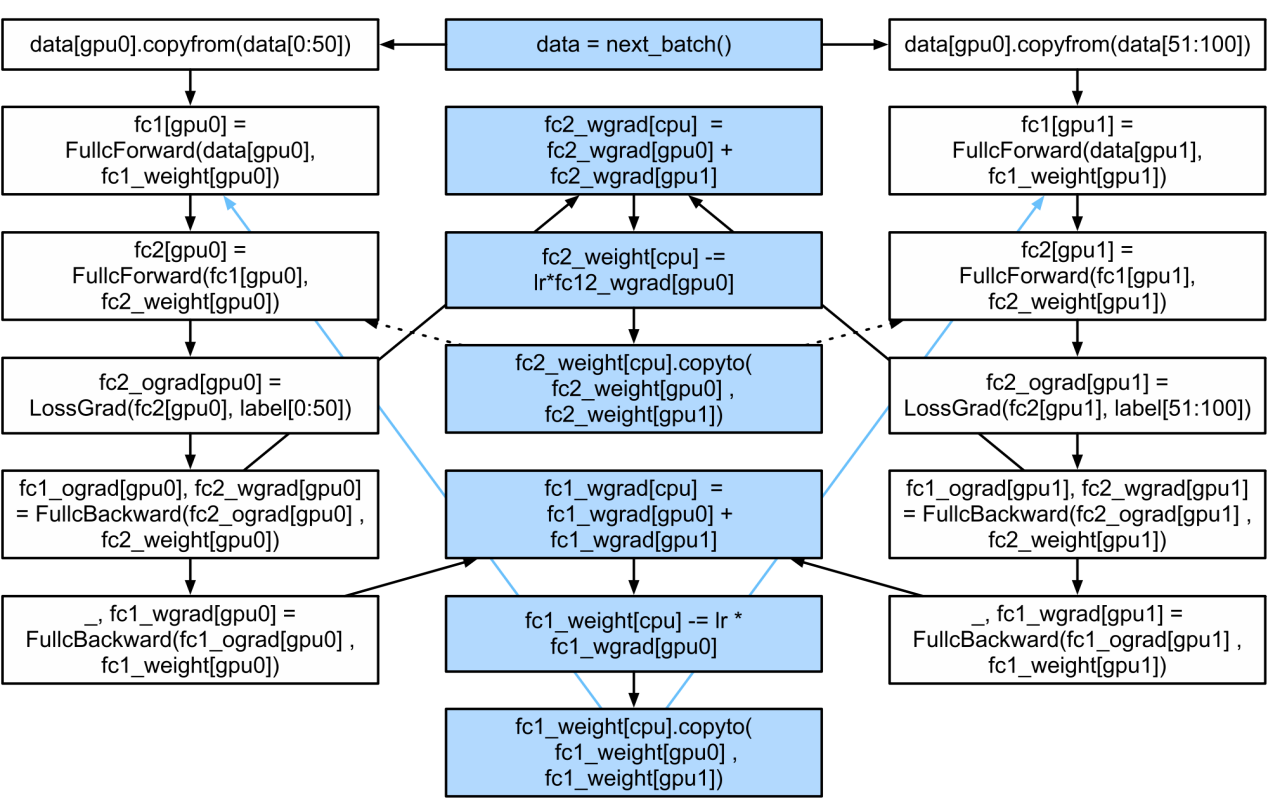
\includegraphics{images/image-0010.png}
\caption{CPU 与双 GPU 上两层 MLP 的计算依赖关系图}
\end{figure}

\hypertarget{ux53c2ux8003ux6587ux732e-33}{%
\subsection{参考文献}\label{ux53c2ux8003ux6587ux732e-33}}

\begin{itemize}
\tightlist
\item
  Aston Zhang, Zachary C. Lipton, Mu Li, Alexander J. Smola. (2023). \href{https://zh.d2l.ai/}{《动手学深度学习》}. Cambridge University Press.
\end{itemize}

\clearpage

\hypertarget{ux591agpuux8ba1ux7b97}{%
\section{多GPU计算}\label{ux591agpuux8ba1ux7b97}}

\hypertarget{ux4e00ux4e09ux79cdux62c6ux5206ux7b56ux7565}{%
\subsection{一、三种拆分策略}\label{ux4e00ux4e09ux79cdux62c6ux5206ux7b56ux7565}}

\begin{enumerate}
\def\labelenumi{\arabic{enumi}.}
\tightlist
\item
  网络拆分（拆分层/网络深度，纵向切分）（Pipeline Parallelism，PP）
\end{enumerate}

（1）原理：将神经网络的不同层分配给不同的GPU。例如，GPU 1处理第 1-10 层，GPU 2处理第11-20层。数据像流水线一样依次流过各个GPU。

（2）优点

能处理超大模型：因为模型的不同部分存在不同GPU上，单个GPU不需要存下整个模型，因此可以训练参数量巨大的模型。

（3）缺点

负载不均衡：层与层之间依赖性强，必须等待上一层计算完才能进行下一层，容易造成GPU空闲（等待），很难保证每一层的计算量恰好让每个GPU都忙碌且同步。

传输瓶颈：层与层之间的数据（激活值、梯度）传输量极大，可能超出GPU之间的带宽限制。

（4）结论：一般不推荐，只有在超大模型预训练中才会用上（和其他方法一起用），而不会用于前向推理（因为相同算力下，此方法最慢，会增加延迟，影响用户体验）。

\begin{enumerate}
\def\labelenumi{\arabic{enumi}.}
\setcounter{enumi}{1}
\tightlist
\item
  层内拆分（拆分通道/宽度，横向切分）（Tensor Parallelism，TP）
\end{enumerate}

（1）原理：将同一层内的计算工作拆分。如对于矩阵乘法Y = W*X，将权重矩阵W切成两半：W\_1和W\_2。GPU 1持有W\_1，计算一部分结果；GPU 2持有W\_2，计算另一部分结果。然后通过极高速的互联（NVLink）瞬间交换数据，把结果加起来，得到完整的token。又如，一个卷积层有k个通道，将其分给k个GPU，每个GPU负责一部分通道的计算。另外，层内拆分不仅是拆权重，长推理中KV Cache的K和V也会这样拆分。

（2）优点

显存线性扩展：显存占用被分摊，随着GPU数量增加，可以处理更宽、参数规模的网络。

性能提升：当权重规模大时，计算性能提升明显。

（3）缺点

极高的同步成本：由于每一层往往都会进行特征重组和交互（比如在卷积中就是通道重构），每一层计算结束都需要汇总所有GPU的结果才能进入下一层（屏障操作），导致大量等待。

通信开销大：需要传输的数据量可能比第一种方法还要大。

（4）结论：一般只用于大模型预训练和推理，单个GPU无法计算或无法在显存中存储全部权重，不得不拆分的情景。对于小模型，由于带宽成本和同步的复杂性，这种方法性价比低。

\begin{enumerate}
\def\labelenumi{\arabic{enumi}.}
\setcounter{enumi}{2}
\tightlist
\item
  数据并行（拆分数据）（Data Parallelism，DP）
\end{enumerate}

（1）原理

模型复制：每个GPU上都保留一份完整的模型参数副本。

数据拆分：将一个大批量（Batch）的数据切分成多个小份，分发给不同的GPU。比如完成100篇文章的掩码预测，每个GPU各自负责10篇（注：这时候GPU内部也是并行生成每篇的第一个词，然后每篇的第二个词，以此类推）；RLHF中，系统从Prompt库里拿出128个问题，GPU 1拿到问题 1-32，GPU 2拿到问题33-64，虽然 GPU 1必须按顺序生成第1个字、第2个字\ldots\ldots 但在同一毫秒内，GPU 1正在同时算它的32个句子的第T个字，GPU 2也是。

独立计算，统一更新：每个GPU独立计算自己那份数据的梯度，然后所有GPU的梯度进行聚合（求和或平均），最后用聚合后的梯度更新所有GPU上的模型参数。如上面RLHF的例子，只有当大家把句子都写完了，要开始算梯度更新模型的时候，才需要停下来互相交换信息。

（2）优点

实现简单：最容易落地，适用于几乎所有情况。

效率高：同步仅在处理完一个小批量后发生，且可以利用梯度计算的时间差进行部分通信掩盖。

吞吐量大：GPU越多，一次能处理的数据量（Batch Size）就越大，训练越快。

（3）缺点

受限于单卡显存：因为每个GPU都要存完整的模型，所以无法训练单卡显存装不下的超大模型。

（4）结论：最常用。随着现代GPU显存的增加，这是目前几乎所有模型在训练和推理中都会采用的方法。

（5）工作流程

分发数据：将一个随机的小批量数据（batch）均匀切分成k份。

局部计算：每个GPU拿着自己分到的数据，计算损失和梯度。

梯度聚合：将k个GPU算出的梯度收集起来进行合并。

梯度广播：将合并后的总梯度重新发回给每个GPU。

参数更新：每个GPU使用相同的总梯度更新自己维护的模型参数，确保所有GPU上的模型始终保持一致。

（6）实践中的关键调整

批量大小：在k个GPU上训练时，由于每个GPU的工作负载与单卡训练时一致，总的批量大小通常扩大k倍。

学习率：由于批量大小变大了，梯度的估计更准确了，通常需要相应地调大习率以加快收敛。

批量规范化：这是一个特例。因为BN依赖于批量的统计信息（均值和方差），直接在单卡上计算可能会因为单卡数据量小而不准确。通常需要调整，比如使用同步BN（SyncBN）或者为每个GPU保留独立的BN参数。

\hypertarget{ux4e8czerozero-redundancy-optimizer}{%
\subsection{二、ZeRO（Zero Redundancy Optimizer）}\label{ux4e8czerozero-redundancy-optimizer}}

这是目前大模型预训练用到的另一技术（DeepSpeed/FSDP核心）。

在标准的数据并行中，每张卡都存一份完整的模型，太浪费显存。ZeRO把模型参数``切开''，每个GPU存一小块。但和层内切分不同的是，TP中每个GPU分别计算``输入\emph{本GPU的参数''，计算完毕后再相加。ZeRO中，GPU 1会先向其他GPU借到所有需要的参数，再进行``输入}完整参数''的计算，算完马上扔掉不属于自己的（节省显存）。

TP 不仅仅是拆分了权重的\textbf{存储}，更重要的是它拆分了\textbf{计算过程}。它改变了矩阵乘法的数学执行方式。

\begin{itemize}
\tightlist
\item
  \textbf{场景}：我们要计算 \(Y = X \times W\)。矩阵 \(W\) 太大。
\item
  \textbf{做法}：

  \begin{itemize}
  \tightlist
  \item
    将 \(W\) 竖着切成两半：\(W_A\) 和 \(W_B\)。
  \item
    GPU 1 拿着 \(W_A\)，计算 \(Y_A = X \times W_A\)。
  \item
    GPU 2 拿着 \(W_B\)，计算 \(Y_B = X \times W_B\)。
  \end{itemize}
\item
  \textbf{关键点}：

  \begin{itemize}
  \tightlist
  \item
    \textbf{时刻都需要}：在计算这一层的整个过程中，GPU 1 和 GPU 2 都在干活。
  \item
    \textbf{通信极其频繁}：算完这一层，必须马上通过 NVLink 进行一次 \texttt{All-Reduce}（汇总），才能得到最终的 \(Y\) 去算下一层。
  \item
    \textbf{目的}：让单次矩阵计算变快，或者解决单卡算不动的问题。
  \end{itemize}
\end{itemize}

ZeRO 本质上还是\textbf{数据并行（Data Parallelism）}。这意味着，逻辑上每张 GPU 应该拥有一个\textbf{完整}的模型副本。但 ZeRO 说：``太浪费了，我们假装每个人都有完整的，但实际上每人只存一部分。''

\begin{itemize}
\tightlist
\item
  \textbf{场景}：我们在做数据并行。GPU 1 负责数据 A，GPU 2 负责数据 B。
\item
  \textbf{做法（以 ZeRO-3 为例）}：

  \begin{itemize}
  \tightlist
  \item
    参数 \(W\) 被切碎，GPU 1 存前半截，GPU 2 存后半截。\textbf{注意：这是静态存储时的状态。}
  \item
    \textbf{计算开始时（前向传播）}：

    \begin{enumerate}
    \def\labelenumi{\arabic{enumi}.}
    \tightlist
    \item
      \textbf{Broadcast（借参数）}：到了第 1 层，GPU 1 发现自己只有一半参数，它立刻向 GPU 2 要另一半。GPU 2 同理。
    \item
      \textbf{重组}：此时，GPU 1 和 GPU 2 的显存里都有了\textbf{完整的第 1 层参数}。
    \item
      \textbf{独立计算}：GPU 1 算自己的数据 A，GPU 2 算自己的数据 B。\textbf{注意：这里不是合力算一个矩阵，而是各算各的数据。}
    \item
      \textbf{丢弃}：算完第 1 层，为了省显存，大家把借来的参数马上删掉，只保留自己负责保管的那一小块。
    \end{enumerate}
  \end{itemize}
\item
  \textbf{关键点}：

  \begin{itemize}
  \tightlist
  \item
    \textbf{临时重组}：计算时，参数是完整的。
  \item
    \textbf{通信换显存}：用带宽（反复借参数、扔参数）来换取显存空间。
  \end{itemize}
\end{itemize}

一句话总结：TP 是把``干活''的任务拆分了（大家一起算）；ZeRO 是把``保管''的任务拆分了（大家轮流用）。

\hypertarget{ux4e09ux591aux79cdux65b9ux6cd5ux7684ux6df7ux5408ux4f7fux7528}{%
\subsection{三、多种方法的混合使用}\label{ux4e09ux591aux79cdux65b9ux6cd5ux7684ux6df7ux5408ux4f7fux7528}}

在训练大模型时，我们通常会混合使用多种方法：

\begin{enumerate}
\def\labelenumi{\arabic{enumi}.}
\item
  使用数据并行，根据batch划分数据；
\item
  用层内切分把模型切开（比如8张卡切分一个模型），为了让矩阵乘法能跑得动，且单层计算延迟低；
\item
  再在不同的机器节点之间使用ZeRO，如果不加ZeRO，每组TP在训练时都需要存一份完整的优化器状态（FP32格式的参数备份、动量、方差），其占显存是单纯模型参数的数倍；加了ZeRO，这些状态就可以打散存储在成百上千张卡上。
\item
  必要的时候使用层间切分。
\end{enumerate}

\hypertarget{ux53c2ux8003ux6587ux732e-34}{%
\subsection{参考文献}\label{ux53c2ux8003ux6587ux732e-34}}

\begin{itemize}
\tightlist
\item
  Aston Zhang, Zachary C. Lipton, Mu Li, Alexander J. Smola. (2023). \href{https://zh.d2l.ai/}{《动手学深度学习》}. Cambridge University Press.
\end{itemize}

\clearpage

\hypertarget{f1bux4e0edualpipe}{%
\section{1F1B与DualPipe}\label{f1bux4e0edualpipe}}

\hypertarget{ux4e00ux5206ux5e03ux5f0fux8badux7ec3ux6846ux67b6ux4e2dux7684ux57faux672cux8badux7ec3ux6b65ux9aa4}{%
\subsection{一、分布式训练框架中的基本训练步骤}\label{ux4e00ux5206ux5e03ux5f0fux8badux7ec3ux6846ux67b6ux4e2dux7684ux57faux672cux8badux7ec3ux6b65ux9aa4}}

\begin{enumerate}
\def\labelenumi{\arabic{enumi}.}
\tightlist
\item
  F（Forward）：前向计算
\end{enumerate}

动作：输入数据 \(x\) 经过当前层的算子（如矩阵乘法 \(Wx\)），输出激活值 \(y\)。

公式：

\[
y = f(x, \theta)
\]

关键任务：计算预测结果，并\textbf{缓存（Checkpointing）}中间层的激活值，留给后续反向传播使用。

在流水线并行中：F 的输出需要发送给下一个（Downstream）GPU 节点。

\begin{enumerate}
\def\labelenumi{\arabic{enumi}.}
\setcounter{enumi}{1}
\tightlist
\item
  B（Backward for Input / Activation Gradient）：激活梯度计算
\end{enumerate}

动作：根据上一层传回的梯度 \(\frac{\partial L}{\partial y}\)，计算对\textbf{当前层输入} \(x\) 的梯度。

公式：

\[
\nabla x = \frac{\partial L}{\partial x} = \frac{\partial L}{\partial y} \cdot \frac{\partial y}{\partial x}
\]

关键任务：它是反向传播的``接力棒''。计算出的 \(\nabla x\) 必须立刻传回给上一个（Upstream）GPU 节点，以便那一层继续计算。

地位：在流水线并行中，B 位于\textbf{关键路径（Critical Path）}上。如果 B 算得慢或传输延迟高，整个流水线都会卡住（产生 Bubble）。

\begin{enumerate}
\def\labelenumi{\arabic{enumi}.}
\setcounter{enumi}{2}
\tightlist
\item
  W（Backward for Weights / Parameter Gradient）：权重梯度计算
\end{enumerate}

动作：根据梯度 \(\frac{\partial L}{\partial y}\)，计算对\textbf{当前层参数} \(\theta\) 的梯度。

公式：

\[
\nabla \theta = \frac{\partial L}{\partial \theta} = \frac{\partial L}{\partial y} \cdot \frac{\partial y}{\partial \theta}
\]

关键任务：计算出的 \(\nabla \theta\) 会被存放在梯度缓冲区中，最终由优化器（Optimizer）用于更新模型权重。

地位：\(W\) \textbf{不在关键路径上}。因为 \(\nabla \theta\) 只需要在这一层本地更新，不需要传给其他 Rank 来解开计算依赖。

\hypertarget{ux4e8c1f1b}{%
\subsection{二、1F1B}\label{ux4e8c1f1b}}

假设我们有 4 个 GPU（Rank 0\textasciitilde3），流水线深度 \(PP = 4\)。

\begin{itemize}
\tightlist
\item
  \textbf{对于 Rank 0 来说}：它处理微批次 \(m_1\) 的前向计算（\(F_1\)）非常快。
\item
  \textbf{但是}：\(F_1\) 算完后，必须传给 Rank 1 \(\to\) Rank 2 \(\to\) Rank 3，在 Rank 3 算出 Loss 后，梯度再从 Rank 3 \(\to\) Rank 2 \(\to\) Rank 1，最后才传回 Rank 0。
\item
  \textbf{结论}：当 Rank 0 拿到 \(m_1\) 的梯度准备算反向（\(B_1\)）时，中间已经过去了一段很长的时间。
\end{itemize}

为了不让 GPU 闲着，Rank 0 在等待 \(B_1\) 的梯度传回来的这段时间里，会继续往后算 \(F_2, F_3, F_4, \dots\)。

\begin{itemize}
\tightlist
\item
  \(F_i\)：代表当前正在处理的第 \(i\) 个微批次的前向。
\item
  \(B_{i-k}\)：代表之前某个\textbf{已经跑完一圈回来}的微批次（第 \(i-k\) 个）的反向。
\end{itemize}

这里的 \(k\) 实际上取决于 GPU 所在的 Rank 位置。

\begin{itemize}
\tightlist
\item
  在流水线末端（如 Rank 3），\(F\) 和 \(B\) 靠得很近，\(k\) 很小。
\item
  在流水线顶端（如 Rank 0），\(F\) 和 \(B\) 隔得很远，\(k\) 很大。
\end{itemize}

``气泡''大小：

假设每个阶段（\(F\) 或 \(B\)）耗时为 1 个单位时间：

\begin{enumerate}
\def\labelenumi{\arabic{enumi}.}
\tightlist
\item
  \(T = 0\)：Rank 0 执行 \(F_1\)。
\item
  \(T = PP - 1\)：经过 \(PP - 1\) 跳，\(F_1\) 到达最后一个 Rank 并完成计算，立即算出 Loss。
\item
  \(T = PP\)：最后一个 Rank 开始执行反向计算 \(B_1\)。
\item
  \(T = PP + (PP - 1)\)：梯度经过 \(PP - 1\) 跳，传回 Rank 0。
\item
  \(T = 2PP - 1\)：Rank 0 终于可以开始执行 \(B_1\)。
\end{enumerate}

结论：在 Rank 0 看来，从 \(F_1\) 结束到 \(B_1\) 开始，中间隔了 \(2PP - 2\) 个时间片。

这里有一个概念上的区分：\textbf{单任务延迟} vs \textbf{流水线总气泡}。

\begin{itemize}
\tightlist
\item
  \textbf{总气泡（Bubble）}：指的是在整个训练任务中，所有 GPU 处于``空闲（Idle）''状态的总时间。
\item
  在 1F1B 中，Rank 0 在等待 \(B_1\) 回来的这段时间内，并没有闲着，而是在疯狂地跑 \(F_2, F_3, \dots, F_{PP}\)。
\item
  真正无法掩盖的空闲时间只有：最开始启动时的``热身''和最后结束时的``收尾''。将所有 GPU 的空闲时间相加再平均，每个 GPU 的平均气泡大小确实约为 \((PP - 1) \times (F + B)\)。
\end{itemize}

\hypertarget{ux4e09dualpipe}{%
\subsection{三、DualPipe}\label{ux4e09dualpipe}}

我们将以 \textbf{4 个 GPU（Rank 0-3）}、流水线并行深度 \(PP = 4\) 为例。

\begin{itemize}
\tightlist
\item
  \textbf{正向流（D1）}：数据从 \(R0 \to R1 \to R2 \to R3\)（逻辑层 L1 \(\to\) L8）。
\item
  \textbf{反向流（D2）}：数据从 \(R3 \to R2 \to R1 \to R0\)（逻辑层 L1 \(\to\) L8，注意是镜像的）。
\item
  \textbf{计算拆分}：每个阶段分为 \(F\)（前向）、\(B\)（算输入梯度，传给邻居）、\(W\)（算权重梯度，本地用）。
\end{itemize}

\hypertarget{ux4e00ux53ccux5411ux70edux8eabux9636ux6bb5}{%
\subsubsection{（一）双向热身阶段}\label{ux4e00ux53ccux5411ux70edux8eabux9636ux6bb5}}

\textbf{\(T1\)：双向同时启动}

\begin{itemize}
\tightlist
\item
  Rank 0：\(F_{D1}(m_1)\)
\item
  Rank 1：-
\item
  Rank 2：-
\item
  Rank 3：\(F_{D2}(n_1)\)
\end{itemize}

\textbf{\(T2\)：数据向中间汇聚}

\begin{itemize}
\tightlist
\item
  Rank 0：\(F_{D1}(m_2)\)
\item
  Rank 1：\(F_{D1}(m_1)\)
\item
  Rank 2：\(F_{D2}(n_1)\)
\item
  Rank 3：\(F_{D2}(n_2)\)
\end{itemize}

\textbf{\(T3\)：中间节点开始处理双向流}

\begin{itemize}
\tightlist
\item
  Rank 0：\(F_{D1}(m_3)\)
\item
  Rank 1：\(F_{D1}(m_2)+F_{D2}(n_1)\)
\item
  Rank 2：\(F_{D2}(n_2)+F_{D1}(m_1)\)
\item
  Rank 3：\(F_{D2}(n_3)\)
\end{itemize}

\textbf{\(T4\)：第一批双向流到达两端}

\begin{itemize}
\tightlist
\item
  Rank 0：\(F_{D1}(m_4)+F_{D2}(n_1)\)
\item
  Rank 1：\(F_{D1}(m_3)+F_{D2}(n_2)\)
\item
  Rank 2：\(F_{D2}(n_3)+F_{D1}(m_2)\)
\item
  Rank 3：\(F_{D2}(n_4)+F_{D1}(m_1)\)
\item
  备注：此时 \(m_1\) 到达 \(R3\)，\(n_1\) 到达 \(R0\)。
\end{itemize}

分析：在 \(T4\) 结束时，\(m_1\) 在 \(R3\) 算完了全部前向（逻辑 L1-L8），\(n_1\) 在 \(R0\) 算完了全部前向。从 \(T5\) 开始，系统将产生第一批梯度并进入复杂的对冲阶段。

注意：m1和n1是完全不同的数据批次。

\hypertarget{ux4e8cux7a33ux6001ux9636ux6bb5}{%
\subsubsection{（二）稳态阶段}\label{ux4e8cux7a33ux6001ux9636ux6bb5}}

在稳态下，一个 GPU 并不是按顺序执行，而是通过两个主要的\textbf{并行块（Candidate Blocks）}来工作。在一个完整的稳态步内，它包含以下两个核心对冲：

\textbf{对冲 A：\(F_{D1}\) 与 \(B_{D2}\) 的完全重叠}

\begin{itemize}
\tightlist
\item
  \textbf{计算内容}：GPU 同时启动两个算子：

  \begin{enumerate}
  \def\labelenumi{\arabic{enumi}.}
  \tightlist
  \item
    正向流新批次的前向计算 \(F_{D1}(m_i)\)。
  \item
    反向流老批次的激活梯度计算 \(B_{D2}(n_j)\)。
  \end{enumerate}
\item
  \textbf{通信掩盖}：

  \begin{itemize}
  \tightlist
  \item
    在计算 \(F_{D1}\) 时，后台接收 \(B_{D2}\) 需要的下游梯度。
  \item
    在计算 \(B_{D2}\) 时，后台发送 \(F_{D1}\) 产生的激活值。
  \end{itemize}
\item
  \textbf{结论}：只要计算时间 \(T(F) \approx T(B)\)，这两个算子就能把彼此的通信时间完全吞掉。
\end{itemize}

\textbf{对冲 B：\(F_{D2}\) 与 \(B_{D1}\) 的完全重叠}

\begin{itemize}
\tightlist
\item
  与上述逻辑镜像，处理反向流的前向和正向流的激活梯度。
\end{itemize}

\textbf{步骤 C：填补 \(W\)（Weight Gradient）}

\begin{itemize}
\tightlist
\item
  \textbf{计算}：上述 \(B\) 计算完成后，立即在后台异步算 \(W\)（权重梯度）。
\item
  \textbf{原理}：\(W\) 不影响任何人，它是``计算废料''，哪里有缝隙就塞在哪里。
\end{itemize}

在一个对冲周期（如 \(F_{D1}\) 与 \(B_{D2}\) 对冲）内共有4个通信步骤，都被掩盖在计算时间中：

在 \(F_{D1}\) 计算时：

\begin{itemize}
\item
  \texttt{Send-Backward-D2}：把上一批次算好的 \(n_{j-1}\) 梯度发给右边。
\item
  \texttt{Recv-Backward-D2}：从左边接收本批次 \(n_j\) 的梯度。
\end{itemize}

在 \(B_{D2}\) 计算时：

\begin{itemize}
\item
  \texttt{Send-Forward-D1}：把算好的 \(m_i\) 激活值发给右边。
\item
  \texttt{Recv-Forward-D1}：从左边接收下一批次 \(m_{i+1}\) 的激活值。
\end{itemize}

\hypertarget{ux4e09ux6536ux5c3eux9636ux6bb5}{%
\subsubsection{（三）收尾阶段}\label{ux4e09ux6536ux5c3eux9636ux6bb5}}

当所有微批次的前向都跑完了，GPU 进入纯反向模式。

\begin{enumerate}
\def\labelenumi{\arabic{enumi}.}
\tightlist
\item
  \textbf{处理剩余的 \(B\)}：把最后几个微批次的输入梯度算完并传走。此时已经没有 \(F\) 可以对冲了，但因为 \(PP\) 被分成了两个方向，气泡的绝对时长减半。
\item
  \textbf{全力算 \(W\)}：这是最后的体力活，所有 GPU 并行计算自己负责的层权重更新。
\end{enumerate}

\hypertarget{ux56dbux6c14ux6ce1ux51cfux5c11ux7684ux6838ux5fc3ux539fux56e0}{%
\subsubsection{（四）气泡减少的核心原因}\label{ux56dbux6c14ux6ce1ux51cfux5c11ux7684ux6838ux5fc3ux539fux56e0}}

在 1F1B 中，Rank 0 算出 \(F_1\) 后，要等 \(2(PP - 1)\) 个时间片才能拿到梯度算 \(B_1\)。

\[
T_{\mathrm{wait}} = (PP - 1) \times (F + B)
\]

DualPipe采取了以下方式：

\begin{enumerate}
\def\labelenumi{\arabic{enumi}.}
\tightlist
\item
  \textbf{双向对冲（Bidirectional）}：

  \begin{itemize}
  \tightlist
  \item
    在 1F1B 等待梯度的时间里，DualPipe 让 GPU 去跑``另一个方向''的前向和反向。
  \item
    \textbf{数学逻辑}：将一个 PP 链拆成两个半深度的 PP 链对冲。气泡从 \((PP - 1)\) 变成了 \(\left(\frac{PP}{2} - 1\right)\)。
  \end{itemize}
\item
  \textbf{\(B\) 与 \(W\) 拆分（Zero Bubble 思想）}：

  \begin{itemize}
  \tightlist
  \item
    在传统做法中，反向传播是 \(B + W\)。必须等这两个都算完，梯度才能发给上一个 GPU。
  \item
    DualPipe 算完 \(B\)（只需矩阵乘法的一半工作量）\textbf{立即就把梯度发走}。这样邻居 GPU 就能提前开始干活。
  \item
    \textbf{结果}：关键路径上的等待时间进一步压缩。
  \end{itemize}
\item
  \textbf{完全重叠（Full Overlap）}：

  \begin{itemize}
  \tightlist
  \item
    利用现代 GPU 的双工带宽（NVLink 可以同时全速 Send 和 Recv）。
  \item
    DualPipe 调度算法保证了：\textbf{当 GPU 在做计算时，带宽始终是满的；当带宽在传输时，SM 核心始终在计算。}
  \end{itemize}
\end{enumerate}

\hypertarget{ux4e94ux6298ux53e0ux6d41ux6c34ux7ebfux6280ux672f}{%
\subsubsection{（五）折叠流水线技术}\label{ux4e94ux6298ux53e0ux6d41ux6c34ux7ebfux6280ux672f}}

DualPipe的``代价''是一个GPU需要存两倍的权重。原因：

\begin{quote}
正向流 Direction 1：从 \(Rank_0 \rightarrow Rank_3\)。Rank 0 必须有第 1 层。

反向流 Direction 2：从 \(Rank_3 \rightarrow Rank_0\)。但请注意，反向流也是一个完整的前向-反向过程。如果它从 Rank 3 开始起步，Rank 3 就必须有第 1 层。

这样一来，第 1 层在 Rank 0 和 Rank 3 都有，参数量自然翻倍了。
为了解决这个问题，可以采用``折叠''的方法：
\end{quote}

在折叠架构下，我们不再让 Rank 0 和 Rank 3 都存第 1 层，而是这样分配 Stage：

\begin{longtable}[]{@{}lll@{}}
\toprule
物理 Rank & 负责的逻辑 Stage（1x 参数，不冗余） & 物理位置属性 \\
\midrule
\endhead
Rank 0 & Stage 0（入口）和 Stage 7（出口） & 流水线两头 \\
Rank 1 & Stage 1 和 Stage 6 & \\
Rank 2 & Stage 2 和 Stage 5 & \\
Rank 3 & Stage 3 和 Stage 4 & 流水线折返点 \\
\bottomrule
\end{longtable}

虽然每个 Stage 只存了一份（1x 参数），但因为每个 GPU 现在都手握一个靠前的 Stage（如 S0）和一个靠后的 Stage（如 S7），对冲依然可以发生：

\begin{enumerate}
\def\labelenumi{\arabic{enumi}.}
\tightlist
\item
  任务组合：当 Rank 0 正在处理微批次 \(m_{10}\) 的 Stage 0（前向计算）时，它手里可能正好拿着微批次 \(m_1\) 绕了一圈回来的 Stage 7（前向或反向计算）。
\item
  算子对冲：

  \begin{itemize}
  \tightlist
  \item
    计算 A：\(F_{S_0}\)（新批次的前向）。
  \item
    计算 B：\(B_{S_7}\)（老批次的反向）。
  \end{itemize}
\item
  通信掩盖：

  \begin{itemize}
  \tightlist
  \item
    Rank 0 在发送 \(F_{S_0}\) 给 Rank 1 的同时，正好在接收 Rank 1 传回来的 \(B_{S_7}\) 梯度。
  \end{itemize}
\end{enumerate}

这就是``折叠''的精髓：它利用了流水线的深度（一个微批次从 S0 到 S7 走一圈很慢）创造了时间差，让同一个 GPU 在同一时间处理不同生命周期的任务。
但实际上很多大模型并不一定会用``折叠''的方法，原因有两方面。

\begin{enumerate}
\def\labelenumi{\arabic{enumi}.}
\tightlist
\item
  MoE模型的特点
\end{enumerate}

在一个超大规模 MoE 模型中，模型参数被分为两部分：

\begin{itemize}
\tightlist
\item
  \textbf{共享参数（Shared Parameters）}：包括注意力机制（Attention）、层归一化（LayerNorm）和一些共享的稠密层。
\item
  \textbf{专家参数（Expert Parameters）}：MoE 层中成百上千个独立的专家（MLP 块）。
\end{itemize}

这是最核心的工程实现细节：\textbf{专家参数是不参与流水线镜像冗余的。}

在分布式训练中，我们通常同时使用 PP（Pipeline Parallelism）和 EP（Expert Parallelism）：

\begin{enumerate}
\def\labelenumi{\arabic{enumi}.}
\tightlist
\item
  \textbf{PP 决定了路径}：它决定了微批次在哪几个 GPU 之间流转。
\item
  \textbf{EP 决定了存放}：它决定了某一个具体的专家 \(E_{100}\) 物理上存在在哪块显存里。
\end{enumerate}

在 DualPipe 的双向流中：

\begin{itemize}
\tightlist
\item
  当一个微批次运行到某一层需要调用专家时，它会发起一个 All-to-All 通信，去寻找那个专家所在的物理 GPU。
\item
  无论这个微批次是属于``正向流''还是``反向流''，它去寻找的都是同一个物理地址上的专家。
\item
  \textbf{结论：}专家参数在整个集群里依然只存了一份。DualPipe 只需要在每个 Rank 上多存一份轻量级的共享层参数和路由逻辑（Router）即可。
\end{itemize}

\begin{enumerate}
\def\labelenumi{\arabic{enumi}.}
\setcounter{enumi}{1}
\tightlist
\item
  激活值对显存占用更大
\end{enumerate}

对于超长上下文（Context Length）训练，显存瓶颈往往不是参数（Weights），而是激活值。

\begin{itemize}
\tightlist
\item
  在训练时，为了反向传播，每一层的前向计算结果都要存下来。
\item
  DualPipe 的显存压力：真正让显存紧张的是它同时在跑两个方向的流，这意味着显存里要同时存放 \(m\) 批次和 \(n\) 批次的激活值。
\end{itemize}

但 DeepSeek 巧妙地化解了这一点：

\begin{itemize}
\tightlist
\item
  通过 MLA（Multi-head Latent Attention）大幅压缩了 KV Cache 和激活值的体积。
\item
  配合 Recomputation（激活值重计算）技术，可以在需要时再计算部分激活值，用计算时间换取显存空间。
\item
  相比之下，多存那一套共享参数所占用的几 GB 显存，简直是``洒洒水''。
\end{itemize}

\begin{enumerate}
\def\labelenumi{\arabic{enumi}.}
\setcounter{enumi}{2}
\tightlist
\item
  训练调度方面
\end{enumerate}

带宽压榨：

1x 参数的折叠流水线在调度上非常死板（必须走 V 字型）。而 2x 参数的 DualPipe 拥有两条完全独立且对称的路径，这使得它能百分之百跑满双向 NVLink 带宽，调度灵活性极高。

气泡率的极致追求：

在折叠模型中，由于 \(B\) 和 \(W\) 的依赖关系更复杂，很难做到像 DualPipe 那样几乎``零气泡''。DeepSeek 的目标是把 MFU（模型算力利用率）推向 70\% 以上，2x 冗余是一笔划算的交易。

\hypertarget{ux53c2ux8003ux6587ux732e-35}{%
\subsection{参考文献}\label{ux53c2ux8003ux6587ux732e-35}}

\begin{itemize}
\tightlist
\item
  Narayanan, D., Harlap, A., Phanishayee, A., et al.~(2019). \href{https://dl.acm.org/doi/10.1145/3341301.3359646}{PipeDream: Generalized Pipeline Parallelism for DNN Training}. SOSP 2019.
\item
  DeepSeek-AI. (2024). \href{https://arxiv.org/abs/2412.19437}{DeepSeek-V3 Technical Report}. arXiv:2412.19437.
\end{itemize}

\clearpage


% 生成模型
\hypertarget{ux751fux6210ux6a21ux578b}{%
\chapter{生成模型}\label{ux751fux6210ux6a21ux578b}}

\hypertarget{ux751fux6210ux5bf9ux6297ux7f51ux7edcgans}{%
\section{生成对抗网络（GANs）}\label{ux751fux6210ux5bf9ux6297ux7f51ux7edcgans}}

\hypertarget{ux4e00ux6838ux5fc3ux601dux60f3-2}{%
\subsection{一、核心思想}\label{ux4e00ux6838ux5fc3ux601dux60f3-2}}

生成对抗网络是一个非常巧妙且强大的无监督学习框架，由 Ian Goodfellow 在 2014 年提出。GANs的核心思想是设置一个``二人游戏''。想象一下，我们有两个相互竞争的神经网络：

生成器 (Generator, G)：它的工作是``凭空''创造出看起来很真实的数据（比如，假的毕Z加索画作）。它试图模仿真实数据的分布。

判别器 (Discriminator, D)：它的工作是当一个``鉴定专家''，判断一个输入数据是来自真实数据集（真实的毕加索画作）还是生成器伪造的（假的画作）。

它们通过一种``对抗''的方式共同进化：生成器G努力地学习，试图生成越来越逼真的数据来``欺骗''判别器D；判别器D努力地学习，试图提高自己的鉴别能力，准确``识破''所有来自G的伪造品。这个过程就像一场军备竞赛，最终的理想状态是：生成器G变得非常出色，它造出的``假货''足以以假乱真，后续会证明，这将导致判别器D无法分辨，只能靠猜（即判断为真的概率为 50\%）。

\hypertarget{ux4e8cux76eeux6807ux51fdux6570}{%
\subsection{二、目标函数}\label{ux4e8cux76eeux6807ux51fdux6570}}

\[
\min_G \max_D V(D, G)=\mathbb{E}_{x\sim p_{data}(x)}[\log D(x)] + \mathbb{E}_{z\sim p_z(z)}[\log(1 - D(G(z)))]
\]

\begin{enumerate}
\def\labelenumi{\arabic{enumi}.}
\tightlist
\item
  符号与参与者（The Players）
\end{enumerate}

\begin{itemize}
\tightlist
\item
  \(G\)（生成器）：我们的``伪造者''。它是一个神经网络。
\item
  \(D\)（判别器）：我们的``鉴定专家''。它也是一个神经网络。
\item
  \(x\)：代表一个真实数据（比如一张真实的猫的照片）。
\item
  \(p_{data}(x)\)：真实数据的概率分布（理论上所有真实猫的照片的集合）。\(x \sim p_{data}(x)\) 意味着 \(x\) 是从这个真实数据集中随机抽取的一个样本。
\item
  \(z\)：一个随机噪声向量（通常是从一个简单分布，如高斯分布或均匀分布中采样）。\(z\) 是 \(G\) 创造``灵感''的来源。
\item
  \(p_z(z)\)：噪声向量 \(z\) 的分布。\(z \sim p_z(z)\) 意味着 \(z\) 是从这个噪声分布中随机抽取的一个样本。
\end{itemize}

\begin{enumerate}
\def\labelenumi{\arabic{enumi}.}
\setcounter{enumi}{1}
\tightlist
\item
  网络的输入与输出
\end{enumerate}

\begin{itemize}
\tightlist
\item
  \(G(z)\)：

  \begin{itemize}
  \tightlist
  \item
    输入：噪声 \(z\)。
  \item
    输出：一个``伪造''的数据。\(G\) 试图让 \(G(z)\) 看起来和 \(x\) 一样真实。
  \end{itemize}
\item
  \(D(x)\)：

  \begin{itemize}
  \tightlist
  \item
    输入：一个数据（可能是真实的 \(x\)，也可能是伪造的 \(G(z)\)）。
  \item
    输出：一个介于 0 和 1 之间的概率值。这个值表示 \(D\) 认为这个输入数据是真实的概率。
  \item
    \(D(x)\to 1\) 表示 \(D\) 认为 \(x\) 非常可能是真实的。
  \item
    \(D(x)\to 0\) 表示 \(D\) 认为 \(x\) 非常可能是伪造的。
    这里需要说明的是，对于数据 \(x\)，\(D(x)\) 的真实值服从 0-1 分布，但 \(x\) 的概率分布并不是 0-1 分布。这里运用交叉熵损失时，函数里对应的概率分布应该是 \(D(x)\) 的分布，而不是 \(p_{data}(x)\) 这个 \(x\) 的分布。
  \end{itemize}
\end{itemize}

\(p_{data}(x)\) 则是 \(x\) 本身的概率密度分布，它往往不一定是离散的 \(p(x=\cdots)=\cdots\) 形式，而更可能是一个理论上的、隐式的、未知的概率密度分布，是我们试图用模型去学习和模拟的``目标分布''。比如，想象宇宙中存在一个理想的、完美的函数 \(p_{data}\)，它是所有图片的概率密度函数。如果你给这个函数输入一张非常逼真的、自然的人脸图片，它会输出一个高概率密度 \(0.0001\)；输入一张很怪异的图片，它会输出一个较低的概率值 \(10^{-20}\)。这个 \(p_{data}(x)\) 理论上包含了研究范围内所有``有效''数据（例如所有人脸）的生成规律。

我们虽然没有 \(p_{data}\) 概率密度函数本身，但我们有从这个函数中采样 (Sample) 得到的结果。这个``采样结果''就是你的``训练数据集''，例如，ImageNet 数据集就是 \(p_{data}(x)\)（其中 \(x\) 是``自然图像''）的一组样本。在 GAN 的目标函数中，当看到 \(\mathbb{E}_{x\sim p_{data}(x)}\) 这一项时，它的实际操作含义是：``从你的训练数据集中随机抽取一个 batch 的数据 \(x\)。''我们使用这个经验分布近似 \(p_{data}\)，而随着 GAN 的训练，所谓``逼真''其实就代表 \(G\) 生成的数据（图像）的分布越来越接近给定数据集中的分布。事实上，我们也就认为这是在用端到端的方法近似非常复杂的 \(p_{data}\) 函数。之所以需要 GAN 这样的生成模型，正是因为 \(p_{data}(x)\) 过于复杂，我们无法用传统方法（如最大似然估计）直接对其进行建模，因此只能通过这种``博弈''的方式来间接学习它。

\begin{enumerate}
\def\labelenumi{\arabic{enumi}.}
\setcounter{enumi}{2}
\tightlist
\item
  目标函数的逐项解析
\end{enumerate}

现在我们来看这个函数的两大部分：

\[
V(D,G)=\mathbb{E}_{x\sim p_{data}(x)}[\log D(x)] + \mathbb{E}_{z\sim p_z(z)}[\log(1-D(G(z)))]
\]

\begin{itemize}
\tightlist
\item
  第一项：\(\mathbb{E}_{x\sim p_{data}(x)}[\log D(x)]\)

  \begin{itemize}
  \tightlist
  \item
    含义：这一项衡量的是判别器 \(D\) 正确识别真实数据的能力。
  \item
    \(D\) 的目标（\(\max_D\)）：\(D\) 想要最大化这一项。

    \begin{itemize}
    \tightlist
    \item
      当输入一个真实数据 \(x\) 时，\(D\) 希望自己的输出 \(D(x)\) 尽可能接近 1（即``我确定这是真的''）。
    \item
      当 \(D(x)\to 1\) 时，\(\log D(x)\) 会接近 \(\log(1)=0\)。这是 \(\log\) 函数在其定义域（0 到 1）内的最大值。
    \end{itemize}
  \item
    \(G\) 的目标：\(G\) 对这一项没有控制权，因为它只和真实数据 \(x\) 有关。
  \end{itemize}
\item
  第二项：\(\mathbb{E}_{z\sim p_z(z)}[\log(1-D(G(z)))]\)

  \begin{itemize}
  \tightlist
  \item
    含义：这一项衡量的是判别器 \(D\) 正确识别伪造数据的能力。
  \item
    \(D(G(z))\)：这是 \(D\) 对 \(G\) 生成的假数据 \(G(z)\) 的判断（它认为 \(G(z)\) 是真实的概率）。
  \item
    \(1-D(G(z))\)：这就表示 \(D\) 认为 \(G(z)\) 是伪造的概率。
  \item
    \(D\) 的目标（\(\max_D\)）：\(D\) 想要最大化这一项。

    \begin{itemize}
    \tightlist
    \item
      当输入一个伪造数据 \(G(z)\) 时，\(D\) 希望自己的输出 \(D(G(z))\) 尽可能接近 0（即``我确定这是假的''）。
    \item
      当 \(D(G(z))\to 0\) 时，\(1-D(G(z))\) 接近 1，因此 \(\log(1-D(G(z)))\) 接近 \(\log(1)=0\)。
    \item
      所以，通过让 \(\log D(x)\) 和 \(\log(1-D(G(z)))\) 都趋近于 0，\(D\) 就在最大化 \(V(D,G)\)。
    \end{itemize}
  \item
    \(G\) 的目标（\(\min_G\)）：\(G\) 想要最小化这一项（因为 \(G\) 无法影响第一项）。

    \begin{itemize}
    \tightlist
    \item
      \(G\) 的目标是``欺骗'' \(D\)。它希望 \(D\) 在看到 \(G(z)\) 时，误以为它是真的，即 \(D(G(z))\) 尽可能接近 1。
    \item
      当 \(D(G(z))\to 1\) 时，\(1-D(G(z))\) 接近 0。
    \item
      \(\log(1-D(G(z)))\) 会趋近于 \(\log(0)=-\infty\)。
    \item
      这样，\(G\) 就成功地最小化了 \(V(D,G)\)。
    \end{itemize}
  \end{itemize}
\end{itemize}

\begin{enumerate}
\def\labelenumi{\arabic{enumi}.}
\setcounter{enumi}{3}
\tightlist
\item
  总结：\(\min_G \max_D V(D,G)\)
\end{enumerate}

\begin{itemize}
\tightlist
\item
  \(\max_D V(D,G)\)（判别器的目标）：\(D\) 试图最大化 \(V(D,G)\)。它通过训练，力求做到：

  \begin{enumerate}
  \def\labelenumi{\arabic{enumi}.}
  \tightlist
  \item
    看到真实数据 \(x\)，输出 \(D(x)=1\)。
  \item
    看到伪造数据 \(G(z)\)，输出 \(D(G(z))=0\)。如果 \(D\) 是一个完美的判别器，\(V(D,G)\) 的最大值是 \(0+0=0\)。
  \end{enumerate}
\item
  \(\min_G V(D,G)\)（生成器的目标）：\(G\) 试图最小化 \(V(D,G)\)。它通过训练，力求做到：

  \begin{enumerate}
  \def\labelenumi{\arabic{enumi}.}
  \tightlist
  \item
    生成 \(G(z)\)，让 \(D\) 误判，使得 \(D(G(z))=1\)。当 \(G\) 变得更强时，第二项 \(\log(1-D(G(z)))\) 会被推向 \(-\infty\)。
  \end{enumerate}
\end{itemize}

\begin{enumerate}
\def\labelenumi{\arabic{enumi}.}
\setcounter{enumi}{4}
\tightlist
\item
  目标函数相关拓展
\end{enumerate}

（1）判别器D的目标函数

注意到，这个目标函数 \(V(D, G)\) 的形式与二元交叉熵损失 (Binary Cross-Entropy Loss) 非常相似。把 \(D\) 看作一个二元分类器，真实数据 \((x)\) 的标签为 \(y=1\)；伪造数据 \((G(z))\) 的标签为 \(y=0\)。\(D\) 的目标是最小化分类的交叉熵损失，这等价于最大化我们上面的 \(V(D, G)\)。

\begin{enumerate}
\def\labelenumi{\arabic{enumi}.}
\tightlist
\item
  标准的二元交叉熵（BCE）损失
\end{enumerate}

首先，我们回忆一下标准的二元交叉熵损失函数。它通常用于二元分类问题（比如判断``是''或``否''）。

假设：

\begin{itemize}
\tightlist
\item
  \(y\) 是真实标签（\(y=1\) 表示``真''，\(y=0\) 表示``假''）。
\item
  \(p\) 是你的模型预测 \(y=1\) 的概率。
\end{itemize}

那么，单个样本的 BCE 损失 \(L\) 是：

\[
L(y,p) = -[y\cdot\log(p) + (1-y)\cdot\log(1-p)]
\]

这个公式的含义是：

\begin{itemize}
\tightlist
\item
  如果 \(y=1\)（真实标签为``真''）：损失变为 \(L=-[1\cdot\log(p)+0]=-\log(p)\)。

  \begin{itemize}
  \tightlist
  \item
    为了最小化损失 \(L\)，你需要最大化 \(\log(p)\)，也就是让 \(p\to 1\)。
  \end{itemize}
\item
  如果 \(y=0\)（真实标签为``假''）：损失变为 \(L=-[0+1\cdot\log(1-p)]=-\log(1-p)\)。

  \begin{itemize}
  \tightlist
  \item
    为了最小化损失 \(L\)，你需要最大化 \(\log(1-p)\)，也就是让 \(p\to 0\)。
  \end{itemize}
\end{itemize}

这完全符合我们对分类器的期望。

注意：这里我们的损失项要有两部分：一部分鼓励``把真的分入`真'类别''，真实概率分布为：\(p_{data}\) 满足为 1 时代表符合该类别（``为真''），为 0 时不符合。一部分鼓励``把假的分入`假'类别''，真实概率分布为：\(p_z\) 满足为 1 时代表符合该类别（``为假''），为 0 时不符合。

于是，判别器的总损失可以写成：

\[
L_D = L_{real} + L_{fake} = \mathbb{E}[-\log D(x)] + \mathbb{E}[-\log(1-D(G(z)))]
\]

\[
L_D = -\Bigl(\mathbb{E}[\log D(x)] + \mathbb{E}[\log(1-D(G(z)))]\Bigr)
\]

（为了简洁，我们暂时省略了期望符号 \(\mathbb{E}\) 外的 \(x\sim p_{data}\) 和 \(z\sim p_z\)）

现在，我们再回头看 GANs 的目标函数 \(V(D,G)\)：

\[
V(D,G)=\mathbb{E}[\log D(x)] + \mathbb{E}[\log(1-D(G(z)))]
\]

对比一下 \(L_D\) 和 \(V(D,G)\)，我们能清楚地看到：

\[
V(D,G) = -L_D
\]

（2）生成器G的目标函数

按照原公式，生成器 \(G\) 的目标是最小化 \(\mathbb{E}[\log(1-D(G(z)))]\)。这个目标函数在理论上是完美的，但在实践中，尤其是在训练初期，会引发一个严重的问题：梯度消失 (Vanishing Gradients)。

我们来分析一下为什么：

\begin{enumerate}
\def\labelenumi{\arabic{enumi}.}
\tightlist
\item
  训练初期，\(G\) 很差：一开始，\(G\) 只是一个随机的神经网络，它生成的 \(G(z)\) 都是无意义的噪声（比如一堆雪花点）。
\item
  \(D\) 很容易``碾压'' \(G\)：判别器 \(D\) 的任务很简单：区分``真实的猫''和``一堆雪花点''。\(D\) 会很快学会，并且非常自信地将 \(G\) 生成的 \(G(z)\) 判定为假。
\item
  \(D\) 的输出会发生什么？

  \begin{itemize}
  \tightlist
  \item
    当 \(D\) 看到 \(G(z)\)（雪花点）时，它会非常确定这是假的。
  \item
    因此，\(D(G(z))\) 的输出会非常接近 0。
  \end{itemize}
\item
  \(G\) 的损失函数出了什么问题？

  \begin{itemize}
  \tightlist
  \item
    \(G\) 的损失是 \(L_G=\log(1-D(G(z)))\)。
  \item
    如果 \(D(G(z))\) 接近 0（比如 0.001），\(L_G\) 就会是 \(\log(1-0.001)\approx \log(1)=0\)。
  \item
    这看起来 \(G\) 的损失很``低''（接近 0），但这只是一个假象。真正的问题在于梯度。
  \end{itemize}
\end{enumerate}

让我们看一下 \(G\) 的损失函数 \(L_G=\log(1-p)\) 的图像，其中 \(p=D(G(z))\) 是 \(D\) 的输出：

\begin{itemize}
\tightlist
\item
  X 轴：\(D\) 的输出 \(p\)（从 0 到 1）
\item
  Y 轴：\(G\) 的损失 \(L_G\)
\end{itemize}

注意到：

\begin{itemize}
\tightlist
\item
  当 \(p\) 接近 0 时（也就是 \(D\) 非常自信地判定 \(G(z)\) 为假时），这条曲线非常平坦。
\item
  ``平坦''在微积分中意味着斜率（梯度）接近 0。
\end{itemize}

这就是灾难发生的地方：\(G\) 生成了很差的图像 \(\rightarrow\) \(D\) 自信地将其判为假（\(p\approx 0\)）\(\rightarrow\) \(G\) 得到的损失函数梯度 \(\approx 0\) \(\rightarrow\) \(G\) 无法更新参数，它完全学不到东西。

这个问题被称为``饱和'' (Saturating)：\(G\) 在它最需要学习的时候（即它表现最差的时候）反而学得最慢。

原始论文的作者提出了一个简单而实际的修正方法。

他们建议，不要让 \(G\) 最小化 \(\log(1-D(G(z)))\)，而是让 \(G\) 最大化 \(\log(D(G(z)))\)。

\begin{itemize}
\tightlist
\item
  旧损失（蓝色）：\(\log(1-p)\)。当 \(p \rightarrow 0\) 时，梯度是平坦的（消失）。
\item
  新损失（绿色）：\(-\log(p)\)。当 \(p \rightarrow 0\) 时，梯度极其陡峭（趋向 \(-\infty\)）。
\end{itemize}

这个新的损失函数具有我们正想要的特性：它恰好在 \(G\) 表现最差时（即 \(D(G(z))\) 接近 0 时）提供了巨大而强烈的梯度信号。这使得 \(G\) 在训练一开始就能够快速学习。

但此时其实仍然没有完全解决梯度消失问题。

\[
\nabla_{\theta_g} L_G = \nabla_{\theta_g}[-\log(D(G(z)))]
\]

通过链式法则，我们把它分解成三部分：

\[
\nabla_{\theta_g} L_G =
\frac{d(-\log p)}{dp}
\cdot
\nabla_a D(a)\rvert_{a=G(z)}
\cdot
\nabla_{\theta_g} G(z)
\]

其中 \(p=D(G(z))\) 是 \(D\) 的最终输出，\(a=G(z)\) 是 \(D\) 的输入。三部分分别对应：来自 \(G\) 损失的梯度、来自 \(D\) 内部的梯度、来自 \(G\) 内部的梯度。

Part 1：关注的部分

\[
\frac{d(-\log p)}{dp}=-\frac{1}{p}
\]

\begin{itemize}
\tightlist
\item
  当 \(G\) 很差时，\(p=D(G(z)) \rightarrow 0\)。
\item
  这一项 \(-\frac{1}{p}\) 趋向无穷大。
\item
  也就是说，\(G\) 的损失函数本身正在``拼命地''产生一个巨大的信号。
\end{itemize}

Part 2：``真正消失''的部分

\[
\nabla_a D(a)
\]

也就是 \(\nabla_{G(z)}D(G(z))\)，它表示 \(D\) 的输出概率 \(p\) 相对于 \(D\) 的输入 \(a\) 的梯度。\(D\) 如何输出一个 0 到 1 的概率？它的最后一层是一个 Sigmoid 函数。\(D\) 的目标是把真假拉开；当它变得很强时（不重叠），它会给 \(G(z)\) 一个极低的分数。为了输出 \(p \rightarrow 0\)，Sigmoid 函数的输入（logits）必须是一个很大的负数（比如 -10、-20）。

\begin{figure}[htbp]
\centering
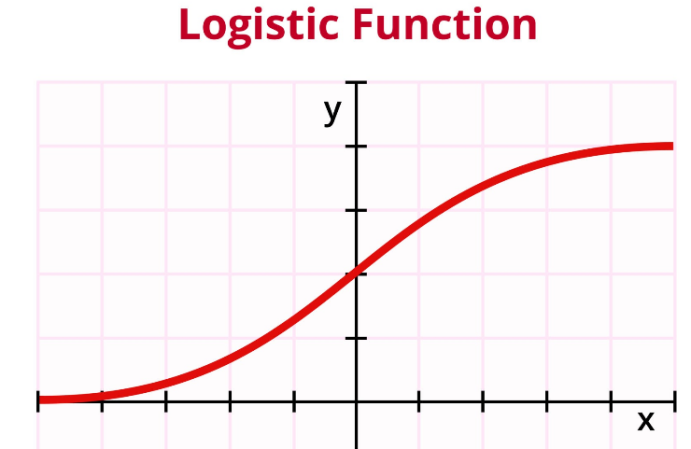
\includegraphics{images/image-0011.png}
\caption{Logistic Function}
\end{figure}

在 \(x\) 很小或很大时，用于把输出转换为概率的 Sigmoid 函数的导数（梯度）趋近于 \(0\)。

\(G\) 的总梯度是：

\[
\nabla_{\theta_g} L_G =
(\mathcjk{趋向无穷大}) \cdot (\mathcjk{趋向 }0) \cdot (\mathcjk{来自 }G\mathcjk{ \mathcjk{的梯度}})
\]

第一项来自 \(\log\)，第二项来自 Sigmoid。
在这个不定型中，Sigmoid函数往往占主导，导致梯度消失。类比就是打开了``消防栓''，但``水管''（D网络）内部被``水垢''（Sigmoid 函数）给堵住了。当D变得很强时，它内部的 Sigmoid 函数会饱和（变得平坦）。这个``平坦''的 Sigmoid 层就像一个被水垢堵住的、极窄的瓶颈（梯度趋于0）。WGAN通过修改D函数，解决了这个问题（见后）。

\hypertarget{ux56dbux8badux7ec3ux7ec8ux70b9}{%
\subsubsection{（四）训练终点}\label{ux56dbux8badux7ec3ux7ec8ux70b9}}

假设我们有一个固定的生成器 \(G\)，我们想找到能最大化 \(V(D,G)\) 的最优判别器 \(D^*\)。

我们的目标函数是：

\[
V(D,G)=\int_x p_{data}(x)\log(D(x))dx+\int_z p_z(z)\log(1-D(G(z)))dz
\]

为了简化，我们知道 \(G(z)\) 会形成一个伪造数据的分布 \(p_g(x)\)，所以我们可以把第二项也写成关于 \(x\) 的积分：

\[
V(D,G)=\int_x [p_{data}(x)\log(D(x))+p_g(x)\log(1-D(x))]dx
\]

要找到使这个积分最大的 \(D(x)\)，我们只需要看积分号里的函数（被积函数），并对任意一个 \(x\) 求它的最大值。

令 \(a=p_{data}(x)\) 和 \(b=p_g(x)\)，我们要找 \(D\) 来最大化 \(f(D)=a\log(D)+b\log(1-D)\)。这是一个标准的求极值问题，我们对 \(D\) 求导并令其为 0：

\[
\frac{df}{dD}=\frac{a}{D}-\frac{b}{1-D}=0
\]

于是：

\[
a=(a+b)D \Rightarrow D=\frac{a}{a+b}
\]

把 \(a\) 和 \(b\) 换回来，我们就得到了最优判别器 \(D^*(x)\)：

\[
D^*(x)=\frac{p_{data}(x)}{p_{data}(x)+p_g(x)}
\]

以上推导通过对D求导，找到了使得V(D,G)最大的D，也就是最优判别器。这个公式告诉我们，一个完美的判别器，其输出概率D(x)应该等于``这个x来自真实数据的概率''除以``它来自真实数据或伪造数据的总概率''。

当然，判别器的训练只是手段，最终训练终点还要看生成器的输出。容易想到，如果 \(G\) 变得完美，伪造数据完全学习了真实数据的分布，\(p_g(x)=p_{data}(x)\)，则 \(D^*(x)=1/2\)。下面我们来严格证明，当判别器 \(D\) 取 \(D^*\) 时，\(\max_D V(D,G)=V(D^*,G)\) 关于 \(G\) 最小等价于取到这种情况。

\[
C(G)=\max_D V(D,G)=V(D^*,G)
\]

\[
C(G)=\mathbb{E}_{x\sim p_{data}}\left[\log\frac{p_{data}}{p_{data}+p_g}\right]
+\mathbb{E}_{x\sim p_g}\left[\log\frac{p_g}{p_{data}+p_g}\right]
\]

注意：这里把 \(p_{data}(x)\) 简写为 \(p_{data}\)，把 \(p_g(x)\) 简写为 \(p_g\)。

经过一点数学变换，这个表达式可以被重写为：

\[
C(G)=2\cdot D_{JSD}(p_{data}\parallel p_g)-2\log 2
\]

\begin{itemize}
\tightlist
\item
  \(D_{JSD}\) 代表 Jensen-Shannon Divergence（JSD，杰森-香农散度）。
\item
  散度（Divergence）是信息论中用来衡量两个概率分布之间差异性的数学工具。
\end{itemize}

\(G\) 的最终目标是 \(\min_G C(G)\)，也就是：

\[
\min_G [2\cdot D_{JSD}(p_{data}\parallel p_g)-2\log 2]
\]

训练生成器 \(G\) 的最终数学目标，就是最小化真实数据分布 \(p_{data}(x)\) 和伪造数据分布 \(p_g(x)\) 之间的 JSD 散度，当且仅当两个分布完全相同时，即 \(p_g(x)=p_{data}(x)\) 时，JSD 散度才为 \(0\)。总之，目标函数中 \(\min_G\) 和 \(\max_D\) 博弈的巧妙设计，使得 \(G\) 的任务变成了学习一个完美的 \(p_g\) 分布，使其与 \(p_{data}\) 一致。

\hypertarget{ux4e09gansux7684ux5e94ux7528}{%
\subsection{三、GANs的应用}\label{ux4e09gansux7684ux5e94ux7528}}

\begin{enumerate}
\def\labelenumi{\arabic{enumi}.}
\tightlist
\item
  图像生成与艺术创作
\end{enumerate}

这是GANs最著名的应用。目标是让模型学习一个庞大数据集（比如10万张人脸照片）的``精髓''，然后能从一个随机噪声向量 \(z\) 出发，生成一张全新的、不属于数据集中任何一张，但又看起来极其逼真的人脸。可以用 StyleGAN、BigGAN 等模型生成不存在的``模特''照片、创造数字艺术、游戏角色设计。

与变分自编码器（Variational Autoencoders, VAEs）相比：

\textbf{GANs}

\begin{itemize}
\tightlist
\item
  核心思想：对抗（Adversarial），一个生成器和一个判别器相互博弈。
\item
  训练目标：欺骗判别器，即 \(G\) 的目标是让 \(D\) 无法区分真假。
\item
  生成质量：高保真（Sharp）。由于 \(D\) 的存在，\(G\) 被迫生成清晰、锐利的图像边缘和纹理，否则很容易被判别为假。
\item
  潜空间 \(z\)：通常较纠缠（Entangled）。原始 GANs 的 \(z\) 空间较无序，改变 \(z\) 的一个维度，可能同时改变人脸的多个特征，如头发、年龄、朝向。
\end{itemize}

\textbf{VAEs}

\begin{itemize}
\tightlist
\item
  核心思想：编码-解码（Encoding-Decoding），编码器将图像压缩成潜空间 \(z\) 中的概率分布，解码器再从 \(z\) 中采样并重建图像。
\item
  训练目标：最小化重建损失，让解码后的图像与原始图像尽可能接近。
\item
  生成质量：较模糊（Blurry）。VAEs 最小化像素级平均误差（如 \(L_2\) 损失），这会鼓励模型生成更``安全''的平均图像。
\item
  潜空间 \(z\)：更平滑（Smooth）。VAEs 的 \(z\) 空间被正则化为连续且平滑的结构，适合在两张人脸的 \(z\) 向量之间做插值。
\end{itemize}

VAEs 擅长学习一个平滑且有意义的潜空间（适合插值和理解数据结构），但生成结果偏模糊。GANs 擅长生成高度逼真的图像（适合追求视觉保真度），但训练更不稳定，潜空间也不如VAEs规整。

\begin{enumerate}
\def\labelenumi{\arabic{enumi}.}
\setcounter{enumi}{1}
\tightlist
\item
  图像到图像的转换
\end{enumerate}

这类应用的目标是：给定一张输入图像 A，将其转换为另一张具有特定风格或特征的输出图像 B。这里，输入和输出都是图像，而且往往在结构上有一定的对应关系。典型模型如 Pix2Pix（需要成对的训练数据，比如一张草图对应一张照片）、CycleGAN（不需要成对数据，通过循环一致性损失实现非配对转换）。应用如将航拍地图转换为谷歌地图样式，将黑白照片上色，将手绘草图转换为逼真照片，将白天场景转换为夜晚场，将物体从语义分割图还原为真实图像等。在这个领域，传统的神经网络架构主要依赖于编码器-解码器（Encoder-Decoder）结构，通常是卷积神经网络（CNNs），并且常常会加入跳跃连接（如 U-Net 结构）来保留细节。

基于 GANs 的方法（如 Pix2Pix、CycleGAN）与基于 CNNs 的编码器-解码器（如 U-Net）相比：

\textbf{基于 GANs 的方法}

\begin{itemize}
\tightlist
\item
  核心思想：学习映射 \(G\) 和判别真假 \(D\)。生成器 \(G\) 学习从 A 域到 B 域的映射，判别器 \(D\) 判断 \(G\) 生成的 B 是否像真实的 B 域图像。
\item
  损失函数：对抗损失加像素级损失。除了让 \(G\) 骗过 \(D\) 的对抗损失外，还会结合 \(L_1\) 或 \(L_2\) 损失，确保生成图像与目标在像素层面相似。
\item
  生成质量：细节更丰富、更真实。判别器 \(D\) 的存在迫使生成器 \(G\) 生成高频细节，使图像在复杂纹理和结构上更逼真、更锐利。
\item
  对数据对的需求：Pix2Pix 需要成对数据；CycleGAN 不需要成对数据，而是通过循环一致性损失学习非配对转换。
\item
  灵活性：高度灵活，可以学习风格迁移、物体转化等非常规映射。CycleGAN 甚至能在没有直接对应样本的情况下进行域转换。
\end{itemize}

\textbf{基于 CNNs 的编码器-解码器}

\begin{itemize}
\tightlist
\item
  核心思想：学习像素级映射。编码器逐步提取特征，解码器逐步重建图像，中间通过跳跃连接传递细节。
\item
  损失函数：通常使用 \(L_1\) 或 \(L_2\) 像素级损失，衡量生成图像和目标图像之间的像素差异。
\item
  生成质量：可能更平滑、更模糊。纯粹的像素级损失（如 \(L_2\)）会倾向于生成像素平均值，导致图像缺乏锐利细节和真实感。
\item
  对数据对的需求：通常需要大量输入 A 与输出 B 的成对数据。
\item
  灵活性：相对受限，主要用于重建、去噪、超分辨率等有明确像素级对应关系的转换。
\end{itemize}

基于 CNNs 的编码器-解码器 方法（如U-Net）在有大量成对数据且任务偏向于结构性恢复（如图像去噪、超分辨率）时表现良好，但可能缺乏真实感。GANs 通过引入判别器，能够生成更具真实感和高频细节的图像，即使在任务更具创意性或缺乏成对数据（如CycleGAN）时也能出色完成。

\begin{enumerate}
\def\labelenumi{\arabic{enumi}.}
\setcounter{enumi}{2}
\tightlist
\item
  数据增强与模拟
\end{enumerate}

有时，我们的真实数据非常少或非常昂贵。如在医学影像（如CT或MRI）中，要诊断一种罕见的癌症。我们可能只有几百张（甚至几十张）带标签的``阳性''图像。如果只用这点数据去训练一个AI模型，它很难学会，而且极易``过拟合''。这时我们往往采取以下方案：

（1）对已有数据进行变换：对于图像而言，就是旋转、裁剪、缩放、翻转、平移、添加噪声、改变对比度或亮度等。

（2）迁移学习：利用预训练模型进行微调。

（3）利用VAE（变分自编码器）：在编码-解码的过程中，一个 VAE 的编码器输出一个概率分布，解码器不是从一个``点''来重建，而是从这个``模糊区域''中随机采样一个点来进行重建。

（4）利用GAN生成：我们可以训练一个基于生成器-判别器架构的GANs模型（比如一个变种的DCGAN或WGAN），判别器以这几百张真实癌症图像的分布为参考基准。一旦训练完成，这个GANs的生成器就可以从随机噪声开始，生成成千上万张看起来逼真、但又与原始图像不完全相同的``假''癌症图像。

这种方法在其他领域也有很多应用。金融中，也可以用其模拟生成逼真的（但非真实的）欺诈交易数据，用于训练反欺诈系统。自动驾驶中，可以生成更多在现实中难以采集的``边缘案例''驾驶场景（如暴风雪中的行人、罕见的交通事故）。

基于 GANs 的数据增强与传统数据增强相比：

\textbf{基于 GANs 的数据增强}

\begin{itemize}
\tightlist
\item
  核心思想：生成新样本（Generation）。模型学习真实数据的潜在分布 \(p_{\mathrm{data}}\)，再从这个分布中采样，创造全新的数据点。
\item
  具体方法：训练一个完整的生成器 \(G\) 来``伪造''数据。
\item
  数据多样性：理论上更高。它能生成原始数据集中不存在、但仍属于同一分布的新组合，例如一个``介于 A 和 B 之间''的新病灶。
\item
  解决的问题：数据稀缺和不平衡。当某一类别的数据（如罕见病）极度稀缺时，GANs 可以补充该类别样本。
\item
  挑战：训练不稳定，容易出现模式崩溃（Mode Collapse），即 \(G\) 只学会生成少数几种``安全''的假样本。
\end{itemize}

\textbf{传统数据增强}

\begin{itemize}
\tightlist
\item
  核心思想：变换旧样本（Transformation）。对已有数据进行简单的几何或颜色变换。
\item
  具体方法：旋转、裁剪、缩放、翻转、平移、添加噪声、改变对比度或亮度。
\item
  数据多样性：相对较低。生成的数据与原始数据高度相关，一张``旋转过的猫''在本质上并没有提供关于``猫''的全新信息。
\item
  解决的问题：缓解过拟合，通过增加训练数据的``表面''数量，使模型看到更多变化，防止它记住特定训练样本。
\item
  挑战：方法简单有效、成本低，但难以创造真正新的类别内变化。
\end{itemize}

\hypertarget{ux53c2ux8003ux6587ux732e-36}{%
\subsection{参考文献}\label{ux53c2ux8003ux6587ux732e-36}}

\begin{itemize}
\tightlist
\item
  Goodfellow, I., Pouget-Abadie, J., Mirza, M., et al.~(2014). \href{https://papers.nips.cc/paper/5423-generative-adversarial-nets}{Generative Adversarial Nets}. NeurIPS 2014.
\end{itemize}

\clearpage

\hypertarget{gansux8badux7ec3ux7684ux6a21ux5f0fux5d29ux6e83ux95eeux9898ux4e0eux89e3ux51b3ux65b9ux6848}{%
\section{GANs训练的模式崩溃问题与解决方案}\label{gansux8badux7ec3ux7684ux6a21ux5f0fux5d29ux6e83ux95eeux9898ux4e0eux89e3ux51b3ux65b9ux6848}}

\hypertarget{ux4e00ux6a21ux5f0fux5d29ux6e83}{%
\subsection{一、模式崩溃}\label{ux4e00ux6a21ux5f0fux5d29ux6e83}}

假设我们正在训练一个 GAN 来生成手写数字（如 MNIST 数据集，包含 0 到 9）。一个成功的 G（生成器）应该能生成所有 10 种不同的、逼真的数字（0, 1, 2, 3, 4, 5, 6, 7, 8, 9）。

如果 \(G\) 和 \(D\) ``对抗实力相同''，并``共同进化''，是不会发生这种情况的。但事实上判别器 \(D\) 在训练早期常学得太快，很快就识别出了 \(G\) 生成的是假的。由于 \(G\) 在各个方向生成得都不好，\(G\) 收到的梯度方向非常混乱，且前面讲述过，\(D\) 函数内部的 Sigmoid 函数会导致 \(p \to 0\) 时梯度消失，这些梯度的幅度比较小。

这时 \(G\) 可能在训练中偶然发现，自己生成的``7''这个数字特别逼真（概率显著大于 \(0\)），每次都能轻易地骗过 \(D\)（判别器）。由于 \(G\) 的唯一目标就是骗过 \(D\)，它会在这一片混乱的梯度中，生成``7''的方向作为唯一稳定的梯度方向，且往往幅度较大。这会把模型引向生成更多``7''的方向，这时便会有更多正反馈，更多梯度让模型进一步导向生成``7''。无论给它什么随机噪声 \(z\) 作为输入，它的输出都是一个（或一小组）看起来差不多的``7''。在这种情况下，我们就说 \(G\) ``崩溃''到了一个单一的模式（数字 ``7''）上，而完全忽略了数据集中的其他所有``模式''（0, 1, 2, 3\ldots）。

\hypertarget{ux4e8cux6a21ux5f0fux5d29ux6e83ux7684ux89e3ux51b3ux65b9ux6848}{%
\subsection{二、模式崩溃的解决方案}\label{ux4e8cux6a21ux5f0fux5d29ux6e83ux7684ux89e3ux51b3ux65b9ux6848}}

\hypertarget{ux4e00wgan}{%
\subsubsection{（一）WGAN}\label{ux4e00wgan}}

WGAN (Wasserstein GAN)，原始 GAN 的``对抗''太激烈了，尤其是判别器 \(D\) 变得太好时，会让生成器 \(G\) 无法学习。为了解决这个问题，WGAN 做了几个关键的改变。

\begin{enumerate}
\def\labelenumi{\arabic{enumi}.}
\tightlist
\item
  改变D的工作和目标函数
\end{enumerate}

原始 GAN 中，\(D\) 是一个分类器 (Classifier)。输出一个 0 到 1 之间的概率（``这是假的'' vs ``这是真的''）；WGAN 中，\(D\) 被重新定义为一个评论家 (Critic)。它不再输出一个概率，而是输出一个分数 (Score)，撤掉了原来的 Sigmoid 函数。这个分数可以（理论上）是任何实数（比如 \(-10, 0, 50\)）。\(D\) 的目标变成了：给真实数据 \(x\) 尽量打高分，给伪造数据 \(G(z)\) 尽量打低分。\(G\) 的目标也随之改变：努力生成 \(G(z)\)，让 \(D\) 给它打出尽可能高的分。

\begin{enumerate}
\def\labelenumi{\arabic{enumi}.}
\setcounter{enumi}{1}
\tightlist
\item
  梯度正则化
\end{enumerate}

\(D\) 的目标变成了给真实数据 \(x\) 尽量打高分，给伪造数据 \(G(z)\) 尽量打低分，但如果一味鼓励拉开高低分，会让 \(D\) 为了拉开高低分而让自己的打分曲线变得``过于陡峭''，导致梯度爆炸。原始方法是权重裁剪 (Weight Clipping)，这是 WGAN 原始论文中提出的方法，强行检查它的每一个权重，如果某个权重超过了一个小范围（比如 \(0.01\)），就把它强行``拉回''到 \(0.01\)；如果低于 \(-0.01\)，就把它``拉回''到 \(-0.01\)。这会导致逐层梯度相乘过程中发生梯度消失 (Vanishing Gradients)，且表达能力受限 (Limited Capacity)：\(D\) 为了满足这个约束，会``偷懒''，把大部分权重都推到边界值（\(0.01\) 或 \(-0.01\)），变成了一个非常简单的函数，只能用``好''或``坏''等词来打分，失去了学习复杂、精细打分曲线的能力。

于是我们选择用如下数学公式作为惩罚项：

\[
\lambda \cdot (\lVert \nabla D(x) \rVert - 1)^2
\]

这就迫使 \(D\) 在训练中必须时时刻刻调整自己的打分曲线，使其在任何地方的``坡度''都尽量保持在 \(1\) 左右。考虑到实际计算开销，我们一般选取真实与伪造的中间点计算惩罚项：

\begin{enumerate}
\def\labelenumi{\arabic{enumi}.}
\item
  取样：我们从数据集中随机取一个真实图像 \(x_{real}\)。
\item
  生成：我们让 \(G\) 生成一个伪造图像 \(x_{fake}\)。
\item
  插值：我们在这两个图像之间随机选择一个``中间点'' \(\hat{x}\)（读作 x-hat）。

  在数学上，我们随机选一个 0 到 1 之间的小数 \(\epsilon\)，然后计算 \(\hat{x}=\epsilon\cdot x_{real}+(1-\epsilon)\cdot x_{fake}\)。这就像在两个点的连线上随机找一个点。
\item
  检查：我们只在这个``中间点'' \(\hat{x}\) 上计算梯度惩罚：
\end{enumerate}

\[
(\lVert \nabla D(\hat{x}) \rVert - 1)^2
\]

为什么这个``中间点''策略有效？想象 \(D\) 的``打分地貌''。我们强迫 \(D\) 在``真实国度''和``伪造国度''之间的整个广阔地带，都必须保持一个平滑的、坡度为 \(1\) 的``山坡''。这使得 \(G\) 无论身处``伪造国度''的哪个角落，都能清晰地看到一条通往``真实国度''的、坡度恒定的上山路径。而在这样的情况下，这个函数在``真实国度''与``伪造国度''的内部梯度极大概率也接近 \(1\)。

\begin{enumerate}
\def\labelenumi{\arabic{enumi}.}
\setcounter{enumi}{2}
\tightlist
\item
  训练终点
\end{enumerate}

我们之前在讨论 GANs 的目标函数时，推导出过这个结论：对于一个固定的 \(G\)，能让 \(V(D,G)\) 最大的那个``最优'' \(D^*\) 是：

\[
D^*(x)=\frac{p_{data}(x)}{p_{data}(x)+p_g(x)}
\]

当 \(G\) 试图最小化 \(\max_D V(D,G)\) 时，它实际上是在最小化 \(C(G)\)：

\[
C(G)=2\cdot JSD(p_{data}\parallel p_g)-2\log 2
\]

所以，\(G\) 的目标（最小化 \(C(G)\)）等价于最小化 \(p_{data}\) 和 \(p_g\) 之间的 JSD 散度。

当 \(p_{data}\) 和 \(p_g\) 完全不重叠时，JSD 会卡在恒定的最大值（\(\log 2\)），其梯度变为 \(0\)。证明：

KL 散度 \(D_{KL}(P\parallel Q)\) 衡量从分布 \(P\) 切换到分布 \(Q\) 时``损失''了多少信息：

\[
D_{KL}(P\parallel Q)=\sum_x P(x)\log\left(\frac{P(x)}{Q(x)}\right)
\]

JSD 散度只是 KL 散度的一个``平滑、对称''版本。首先定义一个``平均分布''：

\[
M=\frac{1}{2}(p_{data}+p_g)
\]

然后：

\[
JSD(p_{data}\parallel p_g)=\frac{1}{2}D_{KL}(p_{data}\parallel M)+\frac{1}{2}D_{KL}(p_g\parallel M)
\]

在``不重叠''的情况下，先看 \(D_{KL}(p_{data}\parallel M)\)：

\[
D_{KL}(p_{data}\parallel M)=\sum_x p_{data}(x)\log\left(\frac{p_{data}(x)}{M(x)}\right)
\]

把 \(M(x)=\frac{1}{2}(p_{data}(x)+p_g(x))\) 代入：

\[
D_{KL}(p_{data}\parallel M)=\sum_x p_{data}(x)\log\left(\frac{p_{data}(x)}{\frac{1}{2}(p_{data}(x)+p_g(x))}\right)
\]

现在，我们只看那些 \(p_{data}(x)>0\) 的点；因为在其他地方 \(p_{data}(x)=0\)，整个求和项都为 0。

在这些点上，由于 \(p_{data}(x)>0\) 且 \(p_g(x)=0\)，所以：

\[
\frac{p_{data}(x)}{\frac{1}{2}(p_{data}(x)+p_g(x))}=2
\]

因此：

\[
D_{KL}(p_{data}\parallel M)=\sum_x p_{data}(x)\log 2=\log 2
\]

同理，\(D_{KL}(p_g\parallel M)=\log 2\)，所以 \(JSD(p_{data}\parallel p_g)=\log 2\)，变成了常数。故 \(C(G)\) 这时为常数，对 \(G\) 的梯度为 0，也就无法驱动生成器 \(G\) 的参数改变。

\hypertarget{ux4e8cux566aux58f0ux6ce8ux5165}{%
\subsubsection{（二）噪声注入}\label{ux4e8cux566aux58f0ux6ce8ux5165}}

``噪声注入'' (Noise Injection) 的原理，就是用来``对抗'' \(G\)（生成器）变得``太确定''、``太死板''的。``模式崩溃''的发生是因为 \(G\) 找到了一个``捷径''：它发现只要生成``7''这个数字，\(D\)（判别器）就没法分辨。于是 \(G\) 就``偷懒''了，无论给它什么输入 \(z\)，它都只生成``7''。从而我们还在``生产线''的中间好几个工序（即 \(G\) 的中间层）上，随机``洒''上一些新的、小的噪声。

它让 \(D\) 的``记忆''失效了。没有抖动时 \(D\) 可能会学会``记住'' \(G\) 生成的那个``完美的7''。它只要看到这个``完美的7''，就给出某个特定的置信度分数。加入噪声后，即使 \(G\) 两次都想生成那个``完美的7''，但由于``抖动''的存在，它两次生成的``7''都会有细微的、随机的差别。\(D\) 被迫去学习数字真正的、普遍的特征（比如它该有的笔画、结构），而不是去记 \(G\) 的某一个``作品''。这反过来又``逼迫'' \(G\) 必须学会生成各种各样、符合模式的、高质量的数字，而不能只依赖一个``捷径''。通过在中间层增加随机性，迫使 \(G\) 学习一个更健壮、更多样化的``生成策略''，从而防止它``崩溃''到一个单一的模式上。

\hypertarget{ux53c2ux8003ux6587ux732e-37}{%
\subsection{参考文献}\label{ux53c2ux8003ux6587ux732e-37}}

\begin{itemize}
\tightlist
\item
  Goodfellow, I., Pouget-Abadie, J., Mirza, M., et al.~(2014). \href{https://papers.nips.cc/paper/5423-generative-adversarial-nets}{Generative Adversarial Nets}. NeurIPS 2014.
\item
  Arjovsky, M., Chintala, S., \& Bottou, L. (2017). \href{https://arxiv.org/abs/1701.07875}{Wasserstein GAN}. ICML 2017.
\end{itemize}

\clearpage

\hypertarget{ux53d8ux5206ux81eaux7f16ux7801ux5668vaeux4e0evq-vae}{%
\section{变分自编码器（VAE）与VQ-VAE}\label{ux53d8ux5206ux81eaux7f16ux7801ux5668vaeux4e0evq-vae}}

\hypertarget{ux4e00vaeux53d8ux5206ux81eaux7f16ux7801ux5668}{%
\subsection{一、VAE（变分自编码器）}\label{ux4e00vaeux53d8ux5206ux81eaux7f16ux7801ux5668}}

\hypertarget{ux4e00ux6838ux5fc3ux601dux60f3ux548cux67b6ux6784}{%
\subsubsection{（一）核心思想和架构}\label{ux4e00ux6838ux5fc3ux601dux60f3ux548cux67b6ux6784}}

\begin{enumerate}
\def\labelenumi{\arabic{enumi}.}
\tightlist
\item
  核心思想：从``确定''到``概率''
\end{enumerate}

传统自编码器的问题：它的编码器直接将输入数据压缩为一个固定的、确定性的潜向量。当你想生成新数据时，从这个潜空间中随机采样一个点，解码出的结果很可能是无意义的噪声，因为你无法保证这个随机点位于模型学习到的数据流形上。

VAE的解决方案：VAE的编码器不再输出一个单一的向量，而是输出一个概率分布，通常是一个高斯分布，由均值（μ）和方差（σ²）两个向量来描述。这意味着对于每一个输入，模型学习的是它在潜空间中的一个可能区域，而不是一个确切点。

根据任务需要，我们可以只取VAE的编码器，或者把编码器和解码器合起来。由于前面所述，解码器需要在概率空间中采样，因此输出不可能与输入完全相同，但输出的统计学分布却会和输入一致。因此把编码器和解码器合起来实际上是一个``模仿器''，它会输出一批和输入分布相同的新数据（因而可用于数据增强等）。

\begin{enumerate}
\def\labelenumi{\arabic{enumi}.}
\setcounter{enumi}{1}
\tightlist
\item
  关键机制：如何学习这个分布？
\end{enumerate}

编码：输入数据~x，编码器输出潜空间中对应的分布参数~μ~和~log(σ²)。

采样：从这个分布~N(μ, σ²)~中随机采样一个潜向量~z。这个步骤是关键的，因为它允许梯度在训练时通过这个随机操作反向传播（通过重参数化技巧）。

解码：将采样的潜向量~z~送入解码器，尝试重建出原始输入~x'。

\begin{enumerate}
\def\labelenumi{\arabic{enumi}.}
\setcounter{enumi}{2}
\tightlist
\item
  损失函数：双重目标
\end{enumerate}

VAE的损失函数由两部分组成，完美体现了其设计思想：

重构损失：衡量解码器输出的重建数据~x'~与原始输入~x~的差异（如均方误差或交叉熵）。这确保了编码后的信息能够有效地还原数据。

KL散度损失：衡量编码器输出的分布~N(μ, σ²)~与先验分布（通常是标准正态分布~N(0, 1)）之间的差异。这个损失项起到了正则化的作用：

它迫使所有编码后的分布都向原点附近聚集，让潜空间变得连续、平滑且有结构。

它避免了编码器``作弊''，比如为每个输入学习一个方差为0的分布（退化成确定性编码），或者把不同的输入编码到相距甚远的区域。

\begin{enumerate}
\def\labelenumi{\arabic{enumi}.}
\setcounter{enumi}{3}
\tightlist
\item
  优势与应用
\end{enumerate}

强大的生成能力：由于潜空间是连续、平滑的，在训练完成后，你可以从先验分布~N(0, 1)~中任意采样一个点，解码器都能生成一个合理、新颖的数据样本（如图像、文本）。

有意义的潜空间：在平滑的潜空间中，进行向量运算（如``微笑的脸'' - ``中性脸'' + ``中性脸'' = ``微笑的脸''）是可能的。

应用：图像生成、数据去噪、缺失数据补全、学习数据的底层流形等。

\hypertarget{ux4e8celboux5bf9ux6570ux4f3cux7136ux53d8ux5206ux4e0bux754c}{%
\subsubsection{（二）ELBO（对数似然变分下界）}\label{ux4e8celboux5bf9ux6570ux4f3cux7136ux53d8ux5206ux4e0bux754c}}

在概率生成模型中，我们通常假设观测数据 \(x\) 是由某种未知的隐变量（Latent Variable）\(z\) 生成的。我们的核心目标是最大化观测数据的边缘似然函数（即对数证据，Log-Evidence）：

\[
\log p(x)=\log\int p(x,z)dz=\log\int p(x\mid z)p(z)dz
\]

这里的困境在于：

\begin{enumerate}
\def\labelenumi{\arabic{enumi}.}
\tightlist
\item
  积分难解（Intractability）：对于复杂的高维模型（如神经网络），隐变量 \(z\) 的空间极其庞大，上述积分无法得到解析解，也无法通过简单的数值计算完成。
\item
  后验难求：根据贝叶斯定理，真实的后验分布为 \(p(z\mid x)=\frac{p(x,z)}{p(x)}\)。因为分母 \(p(x)\)（即上述积分）无法计算，真实的后验分布 \(p(z\mid x)\) 也是不可知的。
\end{enumerate}

为了解决这个问题，变分推断引入了一个易于处理的参数化分布 \(q(z)\)（在 VAE 中通常记作 \(q(z\mid x)\)）来近似真实的后验分布 \(p(z\mid x)\)。

ELBO 就是在这个近似过程中诞生的：既然我们无法直接最大化 \(\log p(x)\)，那我们就去寻找它的一个下界（Lower Bound），通过最大化这个下界，来间接地最大化 \(\log p(x)\)。

我们从近似分布 \(q(z)\) 和真实后验 \(p(z\mid x)\) 之间的 KL 散度（Kullback-Leibler Divergence）出发。KL 散度衡量的是两个分布的差异：

\[
D_{KL}(q(z)\parallel p(z\mid x))=\mathbb{E}_{q(z)}\left[\log\frac{q(z)}{p(z\mid x)}\right]
\]

利用贝叶斯公式 \(p(z\mid x)=\frac{p(x,z)}{p(x)}\)，将其代入上式展开：

\[
D_{KL}(q(z)\parallel p(z\mid x))=\mathbb{E}_{q(z)}\left[\log\frac{q(z)p(x)}{p(x,z)}\right]
\]

利用对数的性质拆分：

\[
D_{KL}(q(z)\parallel p(z\mid x))=\mathbb{E}_{q(z)}[\log q(z)-\log p(x,z)+\log p(x)]
\]

由于 \(\log p(x)\) 是关于观测数据 \(x\) 的常数，与隐变量 \(z\) 无关，我们可以将其从关于 \(q(z)\) 的期望中提取出来：

\[
D_{KL}(q(z)\parallel p(z\mid x))=\mathbb{E}_{q(z)}[\log q(z)-\log p(x,z)]+\log p(x)
\]

整理可得：

\[
\log p(x)=\mathbb{E}_{q(z)}[\log p(x,z)-\log q(z)]+D_{KL}(q(z)\parallel p(z\mid x))
\]

根据 KL 散度的非负性（\(D_{KL}\ge 0\)），我们可以得出：

\[
\log p(x)\ge \mathbb{E}_{q(z)}\left[\log\frac{p(x,z)}{q(z)}\right]
\]

等式右侧的这一项，就是我们要找的对数似然变分下界（ELBO），通常记为 \(\mathcal{L}\)：

\[
ELBO=\mathcal{L}=\mathbb{E}_{q(z)}\left[\log\frac{p(x,z)}{q(z)}\right]
\]

核心推论：由上述等式 \(\log p(x)=ELBO+D_{KL}(q(z)\parallel p(z\mid x))\) 可知，当我们在优化模型（最大化 ELBO）时，由于 \(\log p(x)\) 是固定的数据属性，最大化 ELBO 在数学上严格等价于最小化近似后验 \(q(z)\) 与真实后验 \(p(z\mid x)\) 之间的 KL 散度。这就是为什么通过优化 ELBO 可以让我们的近似分布逼近真实分布。

这个公式非常优美，它将复杂的目标函数拆分成了两个具有极强直观意义的项：

\begin{enumerate}
\def\labelenumi{\arabic{enumi}.}
\tightlist
\item
  重构项（Reconstruction Term）：
\end{enumerate}

\[
\mathbb{E}_{q(z)}[\log p(x \mid z)]
\]

\begin{itemize}
\tightlist
\item
  数学解释：在给定由近似后验 \(q(z)\) 采样出的隐变量 \(z\) 的情况下，模型生成真实数据 \(x\) 的对数似然的期望。
\item
  直观理解：这一项鼓励模型成为一个好的``解码器''。它要求我们提取出的隐特征 \(z\) 必须包含足够的信息，以便能够尽可能完美地还原（重构）出原始输入 \(x\)。在实际代码中，如果 \(x\) 是连续值，这通常对应于均方误差（MSE）；如果是二值化图像，则对应于交叉熵（Cross Entropy）。
\end{itemize}

\begin{enumerate}
\def\labelenumi{\arabic{enumi}.}
\setcounter{enumi}{1}
\tightlist
\item
  正则化项（Regularization Term）：
\end{enumerate}

\[
- D_{KL}(q(z)\parallel p(z))
\]

\begin{itemize}
\tightlist
\item
  数学解释：它是近似后验分布 \(q(z)\) 与先验分布 \(p(z)\)（通常设为标准正态分布 \(\mathcal{N}(0, I)\)）之间的 KL 散度的负值。
\item
  直观理解：这一项起到``信息瓶颈''或正则化的作用。它强制要求我们学习到的隐变量分布 \(q(z)\) 不能过于随意，必须尽量贴合我们预设的先验分布。如果没有这一项，模型可能会简单地记住每一个样本（过拟合），导致隐空间杂乱无章；有了这一项，隐空间会被规范化，从而保证了生成模型具备良好的插值和采样能力。
\end{itemize}

\hypertarget{ux4e8cvq-vaeux5411ux91cfux91cfux5316ux53d8ux5206ux81eaux7f16ux7801ux5668}{%
\subsection{二、VQ-VAE（向量量化变分自编码器）}\label{ux4e8cvq-vaeux5411ux91cfux91cfux5316ux53d8ux5206ux81eaux7f16ux7801ux5668}}

\begin{enumerate}
\def\labelenumi{\arabic{enumi}.}
\tightlist
\item
  核心思想：从连续到离散
\end{enumerate}

VAE学习的是一个连续的潜空间，而VQ-VAE则学习一个离散的潜空间，也称为``代码本''（Codebook）。里边存的是什么：存储着K个``原型特征向量''。每一行向量都代表了一种基础的视觉模式。例如，第5行向量可能代表``垂直边缘''，第10行代表``蓝色平滑纹理''，第50行代表``圆弧的一角''。

\begin{enumerate}
\def\labelenumi{\arabic{enumi}.}
\setcounter{enumi}{1}
\tightlist
\item
  关键机制：向量量化
\end{enumerate}

和VAE一样，编码器首先将输入数据映射为一个高维向量的高斯分布。但不同于VAE的是，编码器会去查找一个预先定义好的代码本，找到与高斯分布中心最接近的代码向量。这个查找过程就是向量量化。具体到图像处理中：我们输入一个图像（高度H、宽度W、通道数C），我们将图像重新划分为h\emph{w个矩形区域（h\textless H,w\textless W），把这h}w个(H\emph{W}C/(h*w))维向量分别送进VQ-VAE，然后分别转变为Codebook中最相近的向量对应的编码，就得到了图像的embedding编码。

\begin{enumerate}
\def\labelenumi{\arabic{enumi}.}
\setcounter{enumi}{2}
\tightlist
\item
  VQ-VAE的优势与意义
\end{enumerate}

更高质量的离散表示：离散的token通常能更好地捕捉数据中固有的、抽象的语义特征（如物体部分、纹理等），这对于语言、推理等任务非常自然。

与现代生成模型结合：VQ-VAE本身的重建质量可能不是最高的，但它产生的离散token成为了连接视觉与语言模型的桥梁。这些令牌可以被一个强大的自回归模型（如Transformer）来学习建模。

流程：VQ-VAE将图像压缩为离散token序列 -\textgreater{} Transformer学习这些token序列的分布（即学习``图像的语法''）-\textgreater{} 要生成新图像时，Transformer先生成一个合理的token序列 -\textgreater{} VQ-VAE的解码器将这些token解码成像素图像。

代表性应用：DALL-E~的第一代和~OpenAI Jukebox~都使用了VQ-VAE的变体来将图像和音频压缩为离散表示，然后用Transformer进行生成。

\hypertarget{ux53c2ux8003ux6587ux732e-38}{%
\subsection{参考文献}\label{ux53c2ux8003ux6587ux732e-38}}

\begin{itemize}
\tightlist
\item
  Kingma, D. P., \& Welling, M. (2014). \href{https://arxiv.org/abs/1312.6114}{Auto-Encoding Variational Bayes}. ICLR 2014.
\item
  van den Oord, A., Vinyals, O., \& Kavukcuoglu, K. (2017). \href{https://arxiv.org/abs/1711.00937}{Neural Discrete Representation Learning}. NeurIPS 2017.
\end{itemize}

\clearpage


% 图神经网络
\hypertarget{ux56feux795eux7ecfux7f51ux7edc}{%
\chapter{图神经网络}\label{ux56feux795eux7ecfux7f51ux7edc}}

\hypertarget{ux56feux795eux7ecfux7f51ux7edc-1}{%
\section{图神经网络}\label{ux56feux795eux7ecfux7f51ux7edc-1}}

\hypertarget{ux4e00ux56feux795eux7ecfux7f51ux7edcgnnux7684ux57faux672cux539fux7406}{%
\subsection{一、图神经网络（GNN）的基本原理}\label{ux4e00ux56feux795eux7ecfux7f51ux7edcgnnux7684ux57faux672cux539fux7406}}

\hypertarget{ux4e00ux524dux5411ux7b97ux6cd5}{%
\subsubsection{（一）前向算法}\label{ux4e00ux524dux5411ux7b97ux6cd5}}

GNN的核心是消息传递（Message Passing），类比``邻居间传递信息更新认知''。其数学流程分为三步：

\begin{enumerate}
\def\labelenumi{\arabic{enumi}.}
\item
  消息生成：对于连接节点u和节点v的边e(u,v)，可以生成一个``消息''m\_uv。这个消息的生成函数通常会同时考虑节点u的特征h\_u、节点v的特征h\_v以及边e(u,v)的特征f\_e(u,v)。例如，可以表示为~m\_uv = Message(h\_u, f\_e(u,v), h\_v)。
\item
  消息聚合：每个节点v会从其所有邻居节点u接收到消息m\_uv，并将这些消息聚合起来形成一个聚合消息M\_v=Aggregate(\{m\_uv\textbar u∈N(v)\})。聚合函数Aggregate通常是求和、平均或最大值等。
\item
  节点更新：节点v的特征h\_v会根据其自身的旧特征h\_v和聚合消息M\_v进行更新。更新函数可以表示为~h\_v(t+1) = Update(h\_v(t), M\_v(t))。
\end{enumerate}

\hypertarget{ux4e8cux8fedux4ee3ux8fc7ux7a0b}{%
\subsubsection{（二）迭代过程\hspace{0pt}}\label{ux4e8cux8fedux4ee3ux8fc7ux7a0b}}

上述步骤重复~K~次（即~K~层GNN），使节点捕获~K~阶邻居信息：

第1层：可以学习到直接邻居特征。

第2层：邻居在第1层学习到了其邻居特征，故这里能学习到``邻居的邻居''。

注意：层数过多可能导致过平滑（所有节点表示趋同）。

\hypertarget{ux4e09ux53cdux5411ux4f20ux64ad}{%
\subsubsection{（三）反向传播}\label{ux4e09ux53cdux5411ux4f20ux64ad}}

消息生成、聚合和更新的函数通常是由可学习的参数（权重矩阵和偏置项）构成的神经网络（如多层感知机MLP）实现的。在反向传播过程中，这些函数的参数会根据损失函数对模型输出的影响来计算梯度并更新节点特征。

此外，一些先进的模型也允许边特征在消息传递过程中被动态更新。例如，在用多尺度交叉注意力Transformer模型学习分子特征时，分子图的节点特征和边特征都会被转换为可供Transformer层处理的输入嵌入，并在多层Transformer中进行处理。另一个例子是分子内消息传递过程，其中初始状态包含节点特征和与键拉伸、键角相关的边特征，在消息传递的每一层中，节点特征和边特征都会得到更新。更新边特征的方法通常与节点特征的更新类似，例如，可以设计一个函数来根据连接节点的特征和旧的边特征来生成新的边特征，或者利用专门的边注意力机制来加权和更新边特征。

\hypertarget{ux4e8cux56feux795eux7ecfux7f51ux7edcux7684ux5e94ux7528}{%
\subsection{二、图神经网络的应用}\label{ux4e8cux56feux795eux7ecfux7f51ux7edcux7684ux5e94ux7528}}

图神经网络特别适用于处理药物分子图和蛋白质结构图，能够有效捕捉复杂的结构信息和高阶关系。药物由原子（节点）和化学键（边）组成，而蛋白质可以由氨基酸残基（节点）和它们之间的相互作用（边）构成。可以运用图神经网络和其他网络结合，预测药物与分子之间的相互作用。例如，先用图神经网络学习分子特征，再用全连接层预测可能的药物结构。

此外，图神经网络以及结合Transformer和卷积神经网络（如TC-DTA）的模型在预测DTA方面表现出色。这些模型能够从复杂的药物和靶点特征中学习非线性映射，从而预测亲和力值。例如，G-K BertDTA框架结合了图表示学习和语义嵌入，用于预测药物-靶点亲和力。

\hypertarget{ux53c2ux8003ux6587ux732e-39}{%
\subsection{参考文献}\label{ux53c2ux8003ux6587ux732e-39}}

\begin{itemize}
\tightlist
\item
  Scarselli, F., Gori, M., Tsoi, A. C., Hagenbuchner, M., \& Monfardini, G. (2009). \href{https://doi.org/10.1109/TNN.2008.2005605}{The Graph Neural Network Model}. IEEE Transactions on Neural Networks.
\end{itemize}

\clearpage


% 第2部分 强化学习
\part*{第2部分 强化学习}
\addcontentsline{toc}{part}{第2部分 强化学习}


% 强化学习的基本知识
\hypertarget{ux5f3aux5316ux5b66ux4e60ux7684ux57faux672cux77e5ux8bc6}{%
\chapter{强化学习的基本知识}\label{ux5f3aux5316ux5b66ux4e60ux7684ux57faux672cux77e5ux8bc6}}

\hypertarget{ux591aux81c2ux8001ux864eux673aux4e0eux4e0aux7f6eux4fe1ux754cucbux7b97ux6cd5}{%
\section{多臂老虎机与上置信界（UCB）算法}\label{ux591aux81c2ux8001ux864eux673aux4e0eux4e0aux7f6eux4fe1ux754cucbux7b97ux6cd5}}

\hypertarget{ux4e00ux591aux81c2ux8001ux864eux673amulti-armed-banditmab}{%
\subsection{一、多臂老虎机（multi-armed bandit，MAB）}\label{ux4e00ux591aux81c2ux8001ux864eux673amulti-armed-banditmab}}

在多臂老虎机问题（见图 2-1）中，有一个拥有~K根拉杆的老虎机，拉动每一根拉杆都对应一个关于奖励的概率分布R。我们每次拉动其中一根拉杆，就可以从该拉杆对应的奖励概率分布中获得一个奖励r。我们在各根拉杆的奖励概率分布未知的情况下，从头开始尝试，目标是在操作T~次拉杆后获得尽可能高的累积奖励。由于奖励的概率分布是未知的，因此我们需要在``探索拉杆的获奖概率''（探索）和``根据经验选择获奖最多的拉杆''（利用）中进行权衡。``采用怎样的操作策略才能使获得的累积奖励最高''便是多臂老虎机问题。

形式化表述：

多臂老虎机问题可以表示为一个元组 \((\mathcal{A}, \mathcal{R})\)，其中：

\begin{itemize}
\tightlist
\item
  \(\mathcal{A}\) 为动作集合，其中一个动作表示拉动一个拉杆。若多臂老虎机一共有 \(K\) 根拉杆，那么动作空间就是集合 \(\{a_1,\ldots,a_K\}\)，我们用 \(a_t \in \mathcal{A}\) 表示任意一个动作。
\item
  \(\mathcal{R}\) 为奖励概率分布，拉动每一根拉杆的动作 \(a\) 都对应一个奖励概率分布 \(R(r\mid a)\)，不同拉杆的奖励分布通常是不同的。
\end{itemize}

假设每个时间步只能拉动一个拉杆，多臂老虎机的目标为最大化一段时间步 \(T\) 内累积的奖励：

\[
\max \sum_{t=1}^{T} r_t,\qquad r_t \sim R(\cdot\mid a_t).
\]

其中 \(a_t\) 表示在第 \(t\) 时间步拉动某一拉杆的动作，\(r_t\) 表示动作 \(a_t\) 获得的奖励。

对于每一个动作 \(a\)，我们定义其期望奖励为

\[
Q(a)=\mathbb{E}_{r\sim R(\cdot\mid a)}[r].
\]

于是，至少存在一根拉杆，它的期望奖励不小于拉动其他任意一根拉杆，我们将该最优期望奖励表示为

\[
Q^{*}=\max_{a\in\mathcal{A}} Q(a).
\]

为了更加直观地观察某一拉杆的期望奖励与最优拉杆期望奖励之间的差距，我们引入``遗憾''（regret）概念。遗憾定义为当前动作与最优动作期望奖励之差，即

\[
R(a)=Q^{*}-Q(a).
\]

累积遗憾（cumulative regret）即操作 \(T\) 次拉杆后累积的遗憾总量。对于一次完整的 \(T\) 步决策 \(\{a_1,a_2,\ldots,a_T\}\)，累积遗憾为

\[
\mathcal{R}_T=\sum_{t=1}^{T} R(a_t).
\]

MAB 问题的目标是最大化累积奖励，等价于最小化累积遗憾。

为了知道拉动哪一根拉杆能获得更高的奖励，我们需要估计这根拉杆的期望奖励。由于只拉动一次拉杆获得的奖励存在随机性，所以需要多次拉动同一根拉杆，然后计算得到的多次奖励的期望。一个增量式估计流程如下：

\begin{enumerate}
\def\labelenumi{\arabic{enumi}.}
\tightlist
\item
  对于任意 \(a\in\mathcal{A}\)，初始化计数器 \(N(a)=0\) 和期望奖励估计值 \(\hat{Q}(a)=0\)。
\item
  对 \(t=1,\ldots,T\) 循环：

  \begin{itemize}
  \tightlist
  \item
    选取某根拉杆，该动作记为 \(a_t\)。
  \item
    得到奖励 \(r_t\)。
  \item
    更新计数器：\(N(a_t)=N(a_t)+1\)。
  \item
    更新期望奖励估计值：\(\hat{Q}(a_t)\leftarrow \hat{Q}(a_t)+\frac{1}{N(a_t)}[r_t-\hat{Q}(a_t)]\)。
  \end{itemize}
\end{enumerate}

注：如果将所有数求和再除以次数，其缺点是每次更新的时间复杂度和空间复杂度均为 \(O(n)\)。而采用增量式更新，时间复杂度和空间复杂度均为 \(O(1)\)。

一个最简单的策略就是一直采取第一个动作，但这就非常依赖运气的好坏。如果运气绝佳，可能拉动的刚好是能获得最大期望奖励的拉杆，即最优拉杆；但如果运气很糟糕，获得的就有可能是最小的期望奖励。

在多臂老虎机问题中，一个经典的问题就是探索与利用的平衡问题。探索（exploration）是指尝试拉动更多可能的拉杆，这根拉杆不一定会获得最大的奖励，但这种方案能够摸清楚所有拉杆的获奖情况。例如，对于一个 10 臂老虎机，我们要把所有的拉杆都拉动一下才知道哪根拉杆可能获得最大的奖励。利用（exploitation）是指拉动已知期望奖励最大的那根拉杆，由于已知的信息仅仅来自有限次的交互观测，所以当前的最优拉杆不一定是全局最优的。例如，对于一个 10 臂老虎机，我们只拉动过其中 3 根拉杆，接下来就一直拉动这 3 根拉杆中期望奖励最大的那根拉杆，但很有可能期望奖励最大的拉杆在剩下的 7 根当中，即使我们对 10 根拉杆各自都尝试了 20 次，发现 5 号拉杆的经验期望奖励是最高的，但仍然存在着微小的概率---另一根 6 号拉杆的真实期望奖励是比 5 号拉杆更高的。

于是在多臂老虎机问题中，设计策略时就需要平衡探索和利用的次数，使得累积奖励最大化。一个比较常用的思路是在开始时做比较多的探索，在对每根拉杆都有比较准确的估计后，再进行利用。目前已有一些比较经典的算法来解决这个问题，例如epsilon-贪婪算法、上置信界算法和汤普森采样算法等。

\hypertarget{ux4e8cepsilon-ux8d2aux5a6aux7b97ux6cd5}{%
\subsection{二、epsilon-贪婪算法}\label{ux4e8cepsilon-ux8d2aux5a6aux7b97ux6cd5}}

完全贪婪算法即在每一时刻采取期望奖励值最大的动作（拉动拉杆），这就是纯粹的利用，而没有探索。所以我们通常需要对完全贪婪算法进行一些修改，其中比较经典的一种方法为 \(\epsilon\)-贪婪（\(\epsilon\)-Greedy）算法。

\(\epsilon\)-贪婪算法在完全贪婪算法的基础上添加了噪声，每次以概率 \(1-\epsilon\) 选择以往经验中期望奖励值最大的那根拉杆（利用），以概率 \(\epsilon\) 随机选择一根拉杆（探索），公式如下：

\[
a_t=
\begin{cases}
\arg\max\limits_{a\in\mathcal{A}} \hat{Q}(a), & \mathcjk{采样概率 } 1-\epsilon,\\
\mathcjk{从 }\mathcal{A}\mathcjk{ \mathcjk{中随机选择}}, & \mathcjk{采样概率 } \epsilon.
\end{cases}
\]

\hypertarget{ux4e09ux4e0aux7f6eux4fe1ux754cucbux7b97ux6cd5}{%
\subsubsection{（三）上置信界（UCB）算法}\label{ux4e09ux4e0aux7f6eux4fe1ux754cucbux7b97ux6cd5}}

设想这样一种情况：对于一台双臂老虎机，其中第一根拉杆只被拉动过一次；第二根拉杆被拉动过很多次，我们对它的奖励分布已经有了大致的把握。这时你会怎么做？或许你会进一步尝试拉动第一根拉杆，从而更加确定其奖励分布。这种思路主要是基于不确定性，因为此时第一根拉杆只被拉动过一次，它的不确定性很高。一根拉杆的不确定性越大，它就越具有探索的价值，因为探索之后我们可能发现它的期望奖励很大。我们在此引入不确定性度量U(a)，它会随着一个动作被尝试次数的增加而减小。我们可以使用一种基于不确定性的策略来综合考虑现有的期望奖励估值和不确定性，其核心问题是如何估计不确定性。

上置信界（upper confidence bound, UCB）算法是一种经典的基于不确定性的策略算法，它的思想用到了一个非常著名的数学原理：霍夫丁不等式（Hoeffding's inequality）。在霍夫丁不等式中，令 \(X_1,\ldots,X_n\) 为 \(n\) 个独立同分布的随机变量，取值范围为 \([0,1]\)，其经验期望为

\[
\bar{x}_n=\frac{1}{n}\sum_{j=1}^{n} X_j,
\]

则有

\[
\Pr\{\mathbb{E}[X]\ge \bar{x}_n+u\}\le e^{-2nu^{2}}.
\]

现在我们将霍夫丁不等式运用于多臂老虎机问题中。将 \(\hat{Q}_t(a)\) 代入 \(\bar{x}_n\)，不等式中的参数 \(u=\hat{U}_t(a)\) 代表不确定性度量。给定一个概率

\[
p=e^{-2N_t(a)\hat{U}_t(a)^{2}},
\]

根据上述不等式，\(Q_t(a)<\hat{Q}_t(a)+\hat{U}_t(a)\) 至少以概率 \(1-p\) 成立。当 \(p\) 很小时，\(Q_t(a)<\hat{Q}_t(a)+\hat{U}_t(a)\) 就会在很大概率上成立，\(\hat{Q}_t(a)+\hat{U}_t(a)\) 便是期望奖励上界。

此时，上置信界算法便选取期望奖励上界最大的动作：

\[
a_t=\arg\max_{a\in\mathcal{A}}[\hat{Q}_t(a)+\hat{U}_t(a)].
\]

所谓的``误判''（或者说我们在设定 \(p\) 时想要规避的那个``小概率事件''），指的正是：拉杆的真实期望值竟然比``我们观察到的平均值加上不确定性红利''还要高。用数学公式表示，就是当下面这个事件发生时，我们视为``误判''：

\[
Q(a)>\hat{Q}_t(a)+\hat{U}_t(a).
\]

如果我们希望降低``把一个很好的杆误认为不好，错过好的解''的概率 \(p\)，我们就要选择把 \(u\) 放宽，拉高上置信界，从而鼓励更多的探索。

当设定p后，我们可以得出不确定度u的值：

\[
u=\sqrt{\frac{-\ln p}{2n}}.
\]

我们一般设置 \(p=1/t\)。在 \(t\) 较小的时候，鼓励算法先通过少数探索快速找到一个近似最优；在 \(t\) 较大的时候，如果一个臂很久没有被选中（\(n\) 没变），但总时间 \(t\) 增加了，那么它的探索加分项就会变大。这会强行把它的得分拉高，让算法去``再试一次''这个臂，以满足我们随时间日益严苛的置信度要求。否则，臂只要被选中一次，\(u\) 就会减小一点，尽管``冷门臂''的 \(u\) 始终更大，但随着时间推移和 \(n\) 的增大，所有臂的 \(u\) 都会逐渐接近 \(0\)，使得这一项远远小于 \(Q\)，最终不起作用，可能让算法收敛向一个次优解。

这里还可以进一步写成经典的 UCB 形式：

\[
a_t=\arg\max_{a\in\mathcal{A}}[\hat{Q}_t(a)+\sqrt{\frac{2\ln t}{N_t(a)}}].
\]

技术彩蛋：在更严谨的 UCB1 推导中，常取 \(p=t^{-4}\)，由此得到探索项 \(\sqrt{\frac{2\ln t}{N_t(a)}}\)。如果只取 \(p=1/t\)，则 \(\sum_t 1/t\) 发散；而 \(p=t^{-4}\) 对应的级数收敛，更便于从数学上证明遗憾上界。但无论取 \(1/t\) 还是 \(t^{-4}\)，核心都是利用 \(\ln t\) 维持长期探索动力。

\hypertarget{ux56dbux6c64ux666eux68eeux91c7ux6837}{%
\subsection{四、汤普森采样}\label{ux56dbux6c64ux666eux68eeux91c7ux6837}}

\begin{enumerate}
\def\labelenumi{\arabic{enumi}.}
\tightlist
\item
  核心思想
\end{enumerate}

如果说 UCB 是一个严谨的数学家（计算严格的边界，绝不冒险漏掉任何可能性），那么汤普森采样就是一个智慧的赌徒（基于概率分布模拟未来，用随机性来对抗未知）。UCB 是频率学派的方法：它根据观察到的数据计算一个固定的数值（平均值 + 误差项）。汤普森采样则是贝叶斯学派的方法。它的核心逻辑是：我不直接估计拉杆的中奖率是多少，而是维护一个``中奖率的概率分布''。在每一步，我从每根拉杆的分布里随机抽一个数（Sample），假装这个数就是这根拉杆的真实能力，然后选那个抽出来数值最大的拉杆。

对于陌生的拉杆：我不知道它中奖率是多少，所以我认为它可能是0到1之间的任何值（分布很宽，很平）。

对于熟悉的拉杆：我知道它中奖率大概是 80\%，所以我认为它的概率分布主要集中在 0.75 到 0.85 之间（分布很窄，很尖）。

\begin{enumerate}
\def\labelenumi{\arabic{enumi}.}
\setcounter{enumi}{1}
\tightlist
\item
  数学模型：Beta分布
\end{enumerate}

在处理二元奖励（赢/输，\(1/0\)）的老虎机问题时，汤普森采样通常使用 Beta 分布（Beta Distribution）作为共轭先验。

不需要被名字吓到，你只需要记住 Beta 分布有两个参数：\(\alpha\) 和 \(\beta\)。

\[
f(x;\alpha,\beta)=\mathrm{Beta}(\alpha,\beta)
\]

在老虎机场景下，它们的物理含义极其简单：

\begin{itemize}
\tightlist
\item
  \(\alpha\)（Alpha）：代表该拉杆``赢（获得奖励 1）''的次数 \(+1\)。
\item
  \(\beta\)（Beta）：代表该拉杆``输（获得奖励 0）''的次数 \(+1\)。
\end{itemize}

为什么这么做？

Beta 分布的形状决定了我们对拉杆的看法：

\begin{enumerate}
\def\labelenumi{\arabic{enumi}.}
\item
  初始状态（\(\alpha=1,\beta=1\)）：相当于均匀分布。我觉得中奖率在 \([0,1]\) 之间任意一个值的概率都一样。这就是``无知''。
\item
  赢多输少（\(\alpha=100,\beta=10\)）：曲线会在 \(0.9\) 附近高高隆起。这意味着``我很确定它是个好拉杆''。
\item
  尝试极少（\(\alpha=2,\beta=1\)）：曲线比较平缓。这意味着``它可能很好，也可能很差，不确定性很大''。
\item
  算法流程
\end{enumerate}

汤普森采样的步骤非常简洁，不需要像 UCB 那样计算复杂的根号和对数：

\begin{enumerate}
\def\labelenumi{\arabic{enumi}.}
\tightlist
\item
  初始化：给每根拉杆 \(k\) 设定两个计数器 \(\alpha_k=1,\beta_k=1\)。
\item
  循环每一步 \(t\)：

  \begin{itemize}
  \item
    采样（Sample）：对于每一根拉杆 \(k\)，从其对应的分布 \(\mathrm{Beta}(\alpha_k,\beta_k)\) 中随机抽取一个样本值 \(\theta_k\sim \mathrm{Beta}(\alpha_k,\beta_k)\)。
  \item
    选择（Select）：选择 \(\theta_k\) 最大的那根拉杆（记为动作 \(A_t\)）。
  \item
    观察（Observe）：拉动拉杆 \(A_t\)，得到奖励 \(r\)（\(0\) 或 \(1\)）。
  \item
    更新（Update）：更新参数（贝叶斯推断）：

    \begin{itemize}
    \tightlist
    \item
      如果赢了（\(r=1\)）：\(\alpha_{A_t}\leftarrow \alpha_{A_t}+1\)
    \item
      如果输了（\(r=0\)）：\(\beta_{A_t}\leftarrow \beta_{A_t}+1\)
    \end{itemize}
  \end{itemize}
\end{enumerate}

\hypertarget{ux53c2ux8003ux6587ux732e-40}{%
\subsection{参考文献}\label{ux53c2ux8003ux6587ux732e-40}}

\begin{itemize}
\tightlist
\item
  \href{https://hrl.boyuai.com/}{《动手学强化学习》}.
\item
  Auer, P., Cesa-Bianchi, N., \& Fischer, P. (2002). \href{https://link.springer.com/article/10.1023/A:1013689704352}{Finite-time Analysis of the Multiarmed Bandit Problem}. Machine Learning.
\end{itemize}

\clearpage

\hypertarget{ux9a6cux5c14ux53efux592bux8fc7ux7a0b}{%
\section{马尔可夫过程}\label{ux9a6cux5c14ux53efux592bux8fc7ux7a0b}}

首先说明：强化学习是一种训练方法（和监督学习等相对应），而不是一种模型架构或优化算法。

\hypertarget{ux4e00ux9a6cux5c14ux53efux592bux8fc7ux7a0b}{%
\subsection{一、马尔可夫过程}\label{ux4e00ux9a6cux5c14ux53efux592bux8fc7ux7a0b}}

多臂老虎机中，智能体的行动并不对环境产生影响，但真实世界并非如此。我们引入马尔可夫过程的概念。

马尔可夫过程（Markov process）指具有马尔可夫性质的随机过程，也被称为马尔可夫链（Markov chain）。我们通常用元组 \((\mathcal{S},P)\) 描述一个马尔可夫过程，其中 \(\mathcal{S}\) 是有限数量的状态集合，\(P\) 是状态转移矩阵（state transition matrix）。假设一共有 \(n\) 个状态，此时 \(\mathcal{S}=\{s_1,s_2,\ldots,s_n\}\)，状态转移矩阵可以写成：

\[
P=
\begin{bmatrix}
P(s_1\mid s_1) & \cdots & P(s_n\mid s_1)\\
\vdots & \ddots & \vdots\\
P(s_1\mid s_n) & \cdots & P(s_n\mid s_n)
\end{bmatrix}.
\]

矩阵 \(P\) 中第 \(i\) 行第 \(j\) 列元素

\[
P(s_j\mid s_i)=P(S_{t+1}=s_j\mid S_t=s_i)
\]

表示从状态 \(s_i\) 转移到状态 \(s_j\) 的概率。对于任意状态 \(s_i\)，从它出发到达其他状态的概率和必须为 \(1\)，即状态转移矩阵的每一行之和为 \(1\)。

\begin{figure}[htbp]
\centering
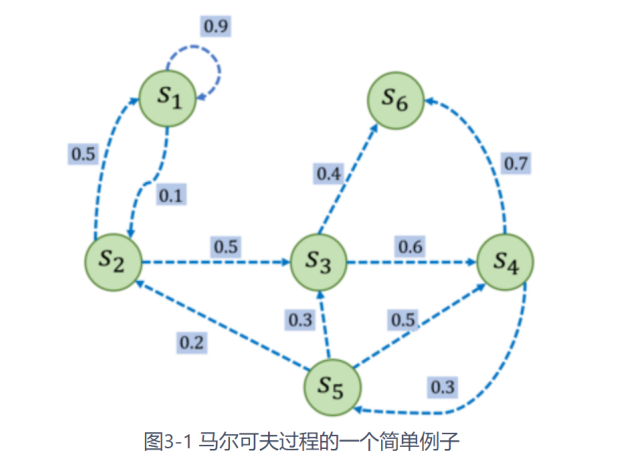
\includegraphics{images/image-0012.png}
\caption{马尔可夫过程状态转移示意图}
\end{figure}

给定一个马尔可夫过程，我们就可以从某个状态出发，根据它的状态转移矩阵生成一个状态序列（episode），这个步骤也被叫作采样（sampling）。例如，从 \(s_1\) 出发，可以生成序列 \(s_1\to s_2\to s_3\to s_6\)，或序列 \(s_1\to s_1\to s_2\to s_3\to s_4\to s_5\to s_3\to s_6\) 等。生成这些序列的概率和状态转移矩阵有关。

\hypertarget{ux4e8cux9a6cux5c14ux53efux592bux5956ux52b1ux8fc7ux7a0b}{%
\subsection{二、马尔可夫奖励过程}\label{ux4e8cux9a6cux5c14ux53efux592bux5956ux52b1ux8fc7ux7a0b}}

\hypertarget{ux56deux62a5}{%
\subsubsection{1. 回报}\label{ux56deux62a5}}

在马尔可夫过程的基础上加入奖励函数 \(r\) 和折扣因子 \(\gamma\)，就可以得到马尔可夫奖励过程（Markov reward process）。一个马尔可夫奖励过程由 \((\mathcal{S},P,r,\gamma)\) 构成，各个组成元素的含义如下：

\begin{itemize}
\tightlist
\item
  \(\mathcal{S}\) 是有限状态集合。
\item
  \(P\) 是状态转移矩阵。
\item
  \(r\) 是奖励函数，某个状态 \(s\) 的奖励 \(r(s)\) 指转移到该状态时可以获得奖励的期望。
\item
  \(\gamma\) 是折扣因子（discount factor），取值范围为 \([0,1)\)。引入折扣因子的原因是远期利益具有一定不确定性，有时我们更希望尽快获得一些奖励，所以会对远期利益进行折扣。\(\gamma\) 接近 \(1\) 时更关注长期累计奖励，接近 \(0\) 时更关注短期奖励。
\end{itemize}

在一个马尔可夫奖励过程中，从第 \(t\) 时刻状态 \(S_t\) 开始，直到终止状态时，所有奖励的衰减之和称为回报 \(G_t\)（return），公式如下：

\[
G_t=R_t+\gamma R_{t+1}+\gamma^{2} R_{t+2}+\cdots
=\sum_{k=0}^{\infty}\gamma^{k} R_{t+k}.
\]

以LLM为例：每次生成就是一次``状态转移''（已有全文即为状态），行动就是从词表（几万个词）中按概率选一个词（token），转移到下一个状态（新的全文）；奖励函数可以对某个状态（结果）或者某个过程进行奖励。

\hypertarget{ux4ef7ux503cux51fdux6570}{%
\subsubsection{2. 价值函数}\label{ux4ef7ux503cux51fdux6570}}

在马尔可夫奖励过程中，一个状态的期望回报（即从这个状态出发的未来累计奖励的期望）被称为这个状态的价值（value）。所有状态的价值组成了价值函数（value function），价值函数的输入为某个状态，输出为这个状态的价值。我们将价值函数写成

\[
V(s)=\mathbb{E}[G_t\mid S_t=s].
\]

进一步展开可得：

\[
\begin{aligned}
V(s)
&=\mathbb{E}[G_t\mid S_t=s]\\
&=\mathbb{E}[R_t+\gamma R_{t+1}+\gamma^{2} R_{t+2}+\cdots\mid S_t=s]\\
&=\mathbb{E}[R_t+\gamma(R_{t+1}+\gamma R_{t+2}+\cdots)\mid S_t=s]\\
&=\mathbb{E}[R_t+\gamma G_{t+1}\mid S_t=s]\\
&=\mathbb{E}[R_t+\gamma V(S_{t+1})\mid S_t=s].
\end{aligned}
\]

在上式的最后一个等号中，一方面，即时奖励的期望正是奖励函数的输出，即 \(\mathbb{E}[R_t\mid S_t=s]=r(s)\)；另一方面，等式中剩余部分 \(\mathbb{E}[\gamma V(S_{t+1})\mid S_t=s]\) 可以根据从状态 \(s\) 出发的转移概率得到，于是得到：

\[
V(s)=r(s)+\gamma\sum_{s'\in\mathcal{S}}P(s'\mid s)V(s').
\]

上式就是马尔可夫奖励过程中非常有名的贝尔曼方程（Bellman equation），对于每一个状态都成立。若一个马尔可夫奖励过程一共有 \(n\) 个状态，即 \(\mathcal{S}=\{s_1,s_2,\ldots,s_n\}\)，我们将所有状态的价值表示成一个列向量 \(\mathbf{V}=[V(s_1),V(s_2),\ldots,V(s_n)]^{\top}\)，同理，转移矩阵 \(P\) 可以写成矩阵形式，奖励函数写成列向量 \(\mathbf{R}=[r(s_1),r(s_2),\ldots,r(s_n)]^{\top}\)。于是贝尔曼方程可以写成：

\[
\mathbf{V}=\mathbf{R}+\gamma P\mathbf{V}.
\]

我们可以直接根据矩阵运算求解：

\[
\begin{aligned}
\mathbf{V}&=\mathbf{R}+\gamma P\mathbf{V},\\
(I-\gamma P)\mathbf{V}&=\mathbf{R},\\
\mathbf{V}&=(I-\gamma P)^{-1}\mathbf{R}.
\end{aligned}
\]

上述解析解的计算复杂度是 \(O(n^{3})\)，其中 \(n\) 是状态个数，因此这种方法只适用于很小的马尔可夫奖励过程。求解较大规模的马尔可夫奖励过程中的价值函数时，可以使用动态规划（dynamic programming）、蒙特卡洛方法（Monte-Carlo method）和时序差分（temporal difference）等方法。

\hypertarget{ux4e09ux9a6cux5c14ux53efux592bux51b3ux7b56ux8fc7ux7a0b}{%
\subsection{三、马尔可夫决策过程}\label{ux4e09ux9a6cux5c14ux53efux592bux51b3ux7b56ux8fc7ux7a0b}}

智能体的策略（policy）通常用字母 \(\pi\) 表示。策略

\[
\pi(a\mid s)=P(A_t=a\mid S_t=s)
\]

是一个函数，表示在输入状态 \(s\) 的情况下采取动作 \(a\) 的概率。当一个策略是确定性策略（deterministic policy）时，它在每个状态下只输出一个确定性的动作，即只有该动作的概率为 \(1\)，其他动作的概率为 \(0\)；当一个策略是随机性策略（stochastic policy）时，它在每个状态下输出的是关于动作的概率分布，然后根据该分布进行采样就可以得到一个动作。

在 MDP 中，由于马尔可夫性质的存在，策略只需要与当前状态有关，不需要考虑历史状态。回顾在 MRP 中的价值函数，在 MDP 中也同样可以定义类似的价值函数。但此时的价值函数与策略有关，这意味着对于两个不同的策略来说，它们在同一个状态下的价值也可能是不同的：不同策略会采取不同动作，从而之后会遇到不同状态并获得不同奖励，所以它们的累积奖励期望也就不同。

我们用 \(V^{\pi}(s)\) 表示在 MDP 中基于策略 \(\pi\) 的状态价值函数（state-value function），定义为从状态 \(s\) 出发遵循策略 \(\pi\) 能获得的期望回报：

\[
V^{\pi}(s)=\mathbb{E}_{\pi}[G_t\mid S_t=s].
\]

不同于 MRP，在 MDP 中由于动作的存在，我们还可以定义动作价值函数（action-value function）。我们用 \(Q^{\pi}(s,a)\) 表示在 MDP 遵循策略 \(\pi\) 时，对当前状态 \(s\) 执行动作 \(a\) 得到的期望回报：

\[
Q^{\pi}(s,a)=\mathbb{E}_{\pi}[G_t\mid S_t=s,A_t=a].
\]

状态价值函数和动作价值函数之间的关系为：在使用策略 \(\pi\) 时，状态 \(s\) 的价值等于在该状态下基于策略 \(\pi\) 采取所有动作的概率与相应动作价值相乘再求和的结果：

\[
V^{\pi}(s)=\sum_{a\in\mathcal{A}}\pi(a\mid s)Q^{\pi}(s,a).
\]

使用策略 \(\pi\) 时，状态 \(s\) 下采取动作 \(a\) 的价值等于即时奖励加上经过衰减后的所有可能下一状态的价值期望：

\[
Q^{\pi}(s,a)=r(s,a)+\gamma\sum_{s'\in\mathcal{S}}P(s'\mid s,a)V^{\pi}(s').
\]

\hypertarget{ux56dbux8d1dux5c14ux66fcux671fux671bux65b9ux7a0b}{%
\subsection{四、贝尔曼期望方程}\label{ux56dbux8d1dux5c14ux66fcux671fux671bux65b9ux7a0b}}

在贝尔曼方程中加上``期望''二字，是为了与接下来的贝尔曼最优方程进行区分。通过简单推导即可分别得到状态价值函数和动作价值函数的贝尔曼期望方程（Bellman expectation equation）：

\[
\begin{aligned}
V^{\pi}(s)
&=\mathbb{E}_{\pi}[R_t+\gamma V^{\pi}(S_{t+1})\mid S_t=s]\\
&=\sum_{a\in\mathcal{A}}\pi(a\mid s)
(r(s,a)+\gamma\sum_{s'\in\mathcal{S}}P(s'\mid s,a)V^{\pi}(s')),
\end{aligned}
\]

\[
\begin{aligned}
Q^{\pi}(s,a)
&=\mathbb{E}_{\pi}[R_t+\gamma Q^{\pi}(S_{t+1},A_{t+1})\mid S_t=s,A_t=a]\\
&=r(s,a)+\gamma\sum_{s'\in\mathcal{S}}P(s'\mid s,a)
\sum_{a'\in\mathcal{A}}\pi(a'\mid s')Q^{\pi}(s',a').
\end{aligned}
\]

\hypertarget{ux4e94ux8d1dux5c14ux66fcux6700ux4f18ux65b9ux7a0b}{%
\subsection{五、贝尔曼最优方程}\label{ux4e94ux8d1dux5c14ux66fcux6700ux4f18ux65b9ux7a0b}}

强化学习的目标通常是找到一个策略，使得智能体从初始状态出发能够获得最多的期望回报。我们首先定义策略之间的偏序关系：当且仅当对于任意状态 \(s\) 都有 \(V^{\pi}(s)\ge V^{\pi'}(s)\) 时，记 \(\pi\succ \pi'\)。于是在有限状态和动作集合的 MDP 中，至少存在一个策略比其他所有策略都好，或者至少存在一个策略不差于其他所有策略，这个策略就是最优策略（optimal policy）。最优策略可能有很多个，我们都将其表示为 \(\pi^{*}(s)\)。

最优策略都有相同的状态价值函数，我们称之为最优状态价值函数：

\[
V^{*}(s)=\max_{\pi}V^{\pi}(s),\qquad \forall s\in\mathcal{S}.
\]

同理，我们定义最优动作价值函数：

\[
Q^{*}(s,a)=\max_{\pi}Q^{\pi}(s,a),\qquad \forall s\in\mathcal{S},a\in\mathcal{A}.
\]

为了使 \(Q^{\pi}(s,a)\) 最大，我们需要在当前状态动作对 \((s,a)\) 之后都执行最优策略，于是得到了最优状态价值函数和最优动作价值函数之间的关系：

\[
Q^{*}(s,a)=r(s,a)+\gamma\sum_{s'\in\mathcal{S}}P(s'\mid s,a)V^{*}(s').
\]

这与普通策略下的状态价值函数和动作价值函数之间的关系一样。另一方面，最优状态价值是选择此时使最优动作价值最大的那个动作时的状态价值：

\[
V^{*}(s)=\max_{a\in\mathcal{A}}Q^{*}(s,a).
\]

根据 \(V^{*}(s)\) 和 \(Q^{*}(s,a)\) 的关系，我们可以得到贝尔曼最优方程（Bellman optimality equation）：

\[
V^{*}(s)=\max_{a\in\mathcal{A}}\bigl(r(s,a)+\gamma\sum_{s'\in\mathcal{S}}P(s'\mid s,a)V^{*}(s')\bigr).
\]

\[
Q^{*}(s,a)=r(s,a)+\gamma\sum_{s'\in\mathcal{S}}P(s'\mid s,a)
\max_{a'\in\mathcal{A}}Q^{*}(s',a').
\]

我们发现，和贝尔曼期望方程与策略 \(\pi\) 挂钩不同的是，贝尔曼最优方程与策略 \(\pi\) 无关，只与环境的状态转移特征有关。

\hypertarget{ux53c2ux8003ux6587ux732e-41}{%
\subsection{参考文献}\label{ux53c2ux8003ux6587ux732e-41}}

\begin{itemize}
\tightlist
\item
  \href{https://hrl.boyuai.com/}{《动手学强化学习》}.
\end{itemize}

\clearpage

\hypertarget{ux72b6ux6001ux5206ux5e03ux4e0eux5360ux7528ux5ea6ux91cf}{%
\section{状态分布与占用度量}\label{ux72b6ux6001ux5206ux5e03ux4e0eux5360ux7528ux5ea6ux91cf}}

\hypertarget{ux4e00ux72b6ux6001ux5206ux5e03ux548cux5360ux7528ux5ea6ux91cfux7684ux5b9aux4e49}{%
\subsection{一、状态分布和占用度量的定义}\label{ux4e00ux72b6ux6001ux5206ux5e03ux548cux5360ux7528ux5ea6ux91cfux7684ux5b9aux4e49}}

状态分布定义为智能体处于状态 \(s\) 的折扣后概率：

定义了 \(\nu^\pi(s)\)，即在策略 \(\pi\) 下的折扣状态访问分布：

\[
\nu^\pi(s) = (1-\gamma)\sum_{t=0}^{\infty}\gamma^t P_t^\pi(s)
\]

\(P_t^\pi(s)\)：表示在时刻 \(t\)，智能体处于状态 \(s\) 的概率。

\(\gamma\)：折扣因子（Discount Factor），\(0 \le \gamma < 1\)。

\(1-\gamma\)：归一化因子（Normalization Factor）。

进而可以定义占用度量，即智能体在s发出动作a的折扣后概率：

\[
\rho^\pi(s,a) = (1-\gamma)\sum_{t=0}^{\infty}\gamma^t P_t^\pi(s)\pi(a|s)
\]

此时有关系：

\[
\rho^\pi(s,a) = \nu^\pi(s)\pi(a|s)
\]

\hypertarget{ux4e8cux539fux7406ux63a8ux5bfc}{%
\subsection{二、原理推导}\label{ux4e8cux539fux7406ux63a8ux5bfc}}

\begin{enumerate}
\def\labelenumi{\arabic{enumi}.}
\tightlist
\item
  为什么需要折扣因子？
\end{enumerate}

我们通常希望最大化累积折扣回报：

\[
J(\pi) = \mathbb{E}_\pi\left[\sum_{t=0}^{\infty}\gamma^t R(s_t,a_t)\right]
\]

利用期望的线性性质，我们可以把求和号拿到期望外面：

\[
J(\pi) = \sum_{t=0}^{\infty}\gamma^t\mathbb{E}_\pi[R(s_t,a_t)]
\]

\[
J(\pi) = \sum_{t=0}^{\infty}\gamma^t\sum_{s,a}P_t^\pi(s)\pi(a|s)R(s,a)
\]

现在，我们将对于 \(s\) 和 \(a\) 的求和提到最前面：

\[
J(\pi) = \sum_{s,a}R(s,a)\left(\sum_{t=0}^{\infty}\gamma^t P_t^\pi(s)\pi(a|s)\right)
\]

括号中的这一项是未归一化的占用度量。为了让这一项变成概率分布（和为 1），我们乘以并除以 \((1-\gamma)\)：

\[
J(\pi) = \frac{1}{1-\gamma}\sum_{s,a}R(s,a)\left((1-\gamma)\sum_{t=0}^{\infty}\gamma^t P_t^\pi(s)\pi(a|s)\right)
\]

其中括号中的部分就是 \(\rho^\pi(s,a)\)，因此：

\[
J(\pi) = \frac{1}{1-\gamma}\sum_{s,a}\rho^\pi(s,a)R(s,a) = \frac{1}{1-\gamma}\mathbb{E}_{(s,a)\sim\rho^\pi}[R(s,a)]
\]

在强化学习中，我们的目标往往是找到一个好的策略。策略可以用概率分布表示，优化目标正是让回报 \(R\) 在 \(\rho^\pi\) 的概率分布下的数学期望最大化。这样一来，问题就转化为寻找这样的概率分布；状态-动作对在分布中的概率，等于该状态-动作对对总价值的贡献权重，符合我们对马尔可夫决策过程的认知。

\begin{enumerate}
\def\labelenumi{\arabic{enumi}.}
\setcounter{enumi}{1}
\tightlist
\item
  为什么需要归一化因子？
\end{enumerate}

这是一个非常关键的数学细节。我们需要证明 \(\nu^\pi(s)\) 是一个合法的概率分布，即其对所有状态求和必须为 1。

推导如下：我们对所有状态 \(s\) 求和：

\[
\sum_s \nu^\pi(s) = \sum_s\left[(1-\gamma)\sum_{t=0}^{\infty}\gamma^t P_t^\pi(s)\right]
\]

交换求和顺序（假设级数收敛）：

\[
= (1-\gamma)\sum_{t=0}^{\infty}\gamma^t\left(\sum_s P_t^\pi(s)\right)
\]

因为无论 \(t\) 是多少，智能体一定会在某个状态，所以 \(\sum_s P_t^\pi(s)=1\)。公式变为：

\[
= (1-\gamma)\sum_{t=0}^{\infty}\gamma^t \cdot 1 = 1
\]

\hypertarget{ux4e09ux5360ux7528ux5ea6ux91cfux7684ux6570ux5b66ux542bux4e49ux6309ux51e0ux4f55ux5206ux5e03ux5728ux65f6ux95f4ux4e0aux91c7ux6837}{%
\subsection{三、占用度量的数学含义：按几何分布在时间上采样}\label{ux4e09ux5360ux7528ux5ea6ux91cfux7684ux6570ux5b66ux542bux4e49ux6309ux51e0ux4f55ux5206ux5e03ux5728ux65f6ux95f4ux4e0aux91c7ux6837}}

通常我们理解的``访问概率''，往往指的是长期来看，在所有时间步中，我有百分之多少的时间待在这个状态（即简单的频率统计）。

但加上折扣因子 \(\gamma\) 后，现在的 \(\rho^\pi(s,a)\) 显然不再是简单的``时间频率''了（因为它重前期、轻后期）。

之所以依然称之为``概率''，是因为我们改变了``采样时间 \(t\)''的概率分布。

传统视角（无折扣，\(\gamma=1\)）

你假设每一个时刻 \(t\) 被抽到的概率是相等的（这在无限时间内其实无法实现数学上的均匀分布，通常取极限）。这就导致了我们常说的``平稳分布''（Stationary Distribution），即单纯的时间平均占比。

折扣视角（有折扣，\(\gamma<1\)）

这里的 \(\rho^\pi(s,a)\) 实际上定义了一个新的随机实验。在这个实验中，我们不是随机均匀地抽取一个时刻，而是按照几何分布（Geometric Distribution）来抽取时刻 \(t\)。

采样规则：

\begin{itemize}
\tightlist
\item
  抽到 \(t=0\) 的概率是 \((1-\gamma)\)。
\item
  抽到 \(t=1\) 的概率是 \((1-\gamma)\gamma\)。
\item
  抽到 \(t=2\) 的概率是 \((1-\gamma)\gamma^2\)。
\item
  \ldots{}
\item
  抽到时刻 \(t\) 的概率是 \(P(T=t)=(1-\gamma)\gamma^t\)，其中 \(T\) 表示采样时刻。
\end{itemize}

现在的物理含义是：

如果不确定在哪个时间点观察，而是按照上述``越近越重要''的规则随机抽取一个瞬间，那么在这个瞬间，智能体位于 \((s,a)\) 的概率是多少？

也可以这样理解：

为了更直观地理解，我们可以引入一个随机终止的设定（这也是 \(\gamma\) 最经典的物理意义）：

假设这个游戏不是无限进行的，而是在每一步结束后，上帝会掷一个骰子：

\begin{itemize}
\tightlist
\item
  有 \(\gamma\) 的概率让游戏继续。
\item
  有 \(1-\gamma\) 的概率让游戏突然结束。
\end{itemize}

那么，\(\rho^\pi(s,a)\) 衡量的就是：

当游戏``突然结束''的那一瞬间（Game Over Snapshot），智能体正处于状态 \(s\) 且正在做动作 \(a\) 的概率。

这个解释完美契合了公式：

\begin{itemize}
\tightlist
\item
  游戏恰好在时刻 \(t\) 结束的概率是 \((1-\gamma)\gamma^t\)。
\item
  在时刻 \(t\) 智能体位于 \((s,a)\) 的概率是 \(P_t^\pi(s,a)\)。
\item
  把所有可能结束的时刻加起来，就是终止时看到 \((s,a)\) 的总概率。
\end{itemize}

因为游戏一定会结束（在某一个时刻），所以所有 \((s,a)\) 的这种概率加起来一定等于 1。因此，它是一个完美的概率分布。

\hypertarget{ux56dbux72b6ux6001ux5206ux5e03ux7684ux9012ux5f52ux8868ux793a}{%
\subsection{四、状态分布的递归表示}\label{ux56dbux72b6ux6001ux5206ux5e03ux7684ux9012ux5f52ux8868ux793a}}

当我们计算 \(\nu^\pi(s')\) 时，我们统计的是从 \(t=0\) 到 \(t=\infty\) 的所有时间步中，智能体出现在 \(s'\) 的加权总和。

对于任何一次出现，它发生的时间只有两种可能：

\begin{enumerate}
\def\labelenumi{\arabic{enumi}.}
\tightlist
\item
  它发生在 \(t=0\)：这就是``初始状态''。
\item
  它发生在 \(t>0\)：这就是``从上一时刻转移过来的''。
\end{enumerate}

在 \(s'\) 的总概率 = 作为起点的权重 + 从别处转移来的权重。

\[
\nu^\pi(s') = (1-\gamma)\nu_0(s') + \gamma\int P(s'|s,a)\pi(a|s)\nu^\pi(s)\,ds\,da
\]

第一项 \((1-\gamma)\nu_0(s')\) 是初始贡献，第二项 \(\gamma\int P(s'|s,a)\pi(a|s)\nu^\pi(s)\,ds\,da\) 是转移贡献。

其中 \(\nu_0(s')\) 指的是初始状态下在 \(s'\) 的概率 \(P(s_0=s')\)，和 \(\nu^\pi\) 不是同一个函数。

第一项：\((1-\gamma)\nu_0(s')\)

\begin{itemize}
\tightlist
\item
  含义：智能体在 \(t=0\) 时刻就位于 \(s'\) 的加权概率。
\item
  \(\nu_0(s')\)：初始状态分布，即 \(P(s_0=s')\)。
\item
  \((1-\gamma)\)：这是一个时间权重的归一化系数。
\item
  回忆 \(\nu^\pi\) 的定义：\(\nu^\pi(s)=(1-\gamma)\sum_{t=0}^{\infty}\gamma^t P(s_t=s)\)。
\item
  当 \(t=0\) 时，\(\gamma^0=1\)。
\item
  所以 \(t=0\) 这一时刻对总分布的贡献就是系数 \((1-\gamma)\) 乘以概率 \(\nu_0(s')\)。
\end{itemize}

第二项：\(\gamma\int P(s'|s,a)\pi(a|s)\nu^\pi(s)\,ds\,da\)

\begin{itemize}
\tightlist
\item
  含义：智能体从上一时刻（任意状态 \(s\)）经过一步转移到达 \(s'\) 的加权概率。
\item
  \(\nu^\pi(s)\)：上一时刻在状态 \(s\) 的概率密度。
\item
  \(\pi(a|s)\)：在 \(s\) 选择动作 \(a\) 的概率。
\item
  \(P(s'|s,a)\)：执行 \(a\) 后从 \(s\) 跳到 \(s'\) 的概率。
\item
  \(\int \cdots dsda\)：对所有可能的``前任''状态和动作进行积分（如果是离散空间就是求和 \(\sum\)），把所有流向 \(s'\) 的可能性汇总。
\item
  \(\gamma\)：关键的折扣因子。
\item
  因为从 \(s\) 到 \(s'\) 经过了 1 个时间步。
\item
  如果在上一时刻（比如 \(t\)）的权重是 \(\gamma^t\)，那么到达 \(s'\) 时已经是时刻 \(t+1\)，权重变成了 \(\gamma^{t+1}\)。
\item
  相比于上一时刻，权重衰减了 \(\gamma\) 倍。所以必须乘上 \(\gamma\)。
\end{itemize}

\hypertarget{ux4e94ux5360ux7528ux5ea6ux91cfux76f8ux5173ux5b9aux7406}{%
\subsection{五、占用度量相关定理}\label{ux4e94ux5360ux7528ux5ea6ux91cfux76f8ux5173ux5b9aux7406}}

进一步得出如下两个定理。

定理 1：智能体分别以策略 \(\pi_1\) 和 \(\pi_2\) 与同一个 MDP 交互，得到的占用度量 \(\rho^{\pi_1}\) 和 \(\rho^{\pi_2}\) 满足：

\[
\rho^{\pi_1} = \rho^{\pi_2} \Longleftrightarrow \pi_1 = \pi_2
\]

定理 2：给定一个合法占用度量 \(\rho\)，可生成该占用度量的唯一策略是：

\[
\pi_\rho = \frac{\rho(s,a)}{\sum_{a'}\rho(s,a')}
\]

\hypertarget{ux53c2ux8003ux6587ux732e-42}{%
\subsection{参考文献}\label{ux53c2ux8003ux6587ux732e-42}}

\begin{itemize}
\tightlist
\item
  \href{https://hrl.boyuai.com/}{《动手学强化学习》}.
\end{itemize}

\clearpage

\hypertarget{ux540cux6b65ux66f4ux65b0ux548cux5f02ux6b65ux66f4ux65b0}{%
\section{同步更新和异步更新}\label{ux540cux6b65ux66f4ux65b0ux548cux5f02ux6b65ux66f4ux65b0}}

\hypertarget{ux4e00ux540cux6b65ux66f4ux65b0}{%
\subsection{一、同步更新}\label{ux4e00ux540cux6b65ux66f4ux65b0}}

在训练 ChatGPT、Llama 等大模型时，使用的是 PPO（Proximal Policy Optimization）或其变体。在这个场景下，几乎不存在异步更新。

流程：

\begin{enumerate}
\def\labelenumi{\arabic{enumi}.}
\tightlist
\item
  数据收集（Rollout）：多个 GPU（Workers）并行地让 LLM 生成文本。
\item
  同步等待（Barrier）：系统必须等待所有 GPU 都生成完指定数量的数据（例如每张卡生成 64 个样本）。
\item
  计算梯度（Backward）：基于这批汇总的数据，计算梯度。
\item
  梯度平均（All-Reduce）：使用分布式训练技术（如 DDP - Distributed Data Parallel），将所有显卡上的梯度取平均。
\item
  更新（Update）：所有显卡同时更新模型参数。
\end{enumerate}

\hypertarget{ux4e8cux5f02ux6b65ux66f4ux65b0}{%
\subsection{二、异步更新}\label{ux4e8cux5f02ux6b65ux66f4ux65b0}}

但有的场景下，几十个线程（Workers）在同时进行，它们的速度差异巨大。线程A计算完毕，如果等待线程B，将造成巨大的资源浪费。此时，往往直接将其送进中央服务器，收集到一定量的数据就直接更新模型，不等待线程B。如下面这些场景：

\begin{enumerate}
\def\labelenumi{\arabic{enumi}.}
\tightlist
\item
  AutoML 与神经架构搜索（NAS）------最典型的场景
\end{enumerate}

这是该问题最原本的出处。

\begin{itemize}
\tightlist
\item
  场景描述：AI 负责设计神经网络结构或调整超参数。
\item
  动作 A（快）：训练一个只有 3 层的浅层网络（耗时 30 秒）。
\item
  动作 B（慢）：训练一个 100 层的深层 ResNet（耗时 2 小时）。
\end{itemize}

\begin{enumerate}
\def\labelenumi{\arabic{enumi}.}
\setcounter{enumi}{1}
\tightlist
\item
  AI for Systems（数据库/编译器/系统优化）
\end{enumerate}

这是目前工业界应用 RL 的热点领域，动作时长的方差极大。

\begin{itemize}
\tightlist
\item
  场景 A：数据库参数调优（Knob Tuning）
\item
  动作：修改数据库配置并运行基准测试（Benchmark）。
\item
  差异：修改 \texttt{work\_mem} 可能只需要重启（快）；修改 \texttt{index} 策略可能需要重建索引（极慢，几十分钟）。
\item
  场景 B：编译器优化（Compiler Optimization）
\item
  动作：决定对代码块应用哪种优化 Pass。
\item
  差异：``死代码消除''（瞬时）；``多面体优化''或``循环展开''（可能导致编译时间激增）。
\end{itemize}

A3C算法也是异步更新，但后来研究人员发现不如同步更新的A2C算法。

\hypertarget{ux4e09ux5f02ux6b65ux66f4ux65b0ux7684ux65f6ux95f4ux52a0ux6743}{%
\subsection{三、异步更新的时间加权}\label{ux4e09ux5f02ux6b65ux66f4ux65b0ux7684ux65f6ux95f4ux52a0ux6743}}

\begin{enumerate}
\def\labelenumi{\arabic{enumi}.}
\tightlist
\item
  异步更新遇到的问题
\end{enumerate}

异步更新主要运用于不同动作耗时相差巨大的场景。在标准的分布式强化学习框架中，多个``执行者''（actors）会同时生成不同的代码方案并运行它们，然后将结果（代码、执行结果、奖励）发送给一个``学习者''（learner）来更新模型。在实际场景中，这会产生问题：如在 10 分钟（600秒）内，Actor可以执行120次动作A，只能执行2次动作 B。``学习者（Learner）''收到了120个关于A的梯度更新信号，却只收到了2个关于 B 的信号。模型参数被A的梯度``淹没''了，导致智能体误以为A是最佳策略，从而陷入局部最优。

以上文提到的两个场景为例。在用AI确定神经网络架构时，如果不进行额外调整，AI会疯狂地生成浅层网络，因为能在短时间内刷出大量的梯度更新。虽然深层网络效果好，但因为反馈太慢，被AI``遗忘''了。类似地，在进行System优化时，也会更倾向于用时较短的动作。

从数学上可以这样解释：

梯度更新公式通常为：

\[
\nabla J(\theta)=\mathbb{E}_{a\sim\pi_\theta}\left[\nabla_\theta\log\pi_\theta(a|s)\cdot A(s,a)\right]
\]

其中 \(\pi_\theta\) 是策略分布，\(A(s,a)\) 是优势函数。注意：这里的期望是假设我们按照策略 \(\pi_\theta\) 的概率分布进行采样的。

在异步分布式系统中，数据的生成速率与执行时间 \(\Delta t\) 成反比。实际采样概率 \(P_{sample}(a)\) 不再仅仅等于策略概率 \(\pi(a)\)，而是被时间扭曲了：

\[
P_{sample}(a)\propto \frac{\pi(a)}{\Delta t(a)}
\]

这意味着，耗时短的动作被采样的概率被人为放大了。如果我们直接用收集到的数据进行更新，我们实际上是在优化一个被时间扭曲的目标函数，而不是原本的目标函数。
事实上，使用经验回放池的Off-Policy算法（DQN, SAC, DDPG）理论上也是不同步的，Worker 只管往池子里扔数据（可以是异步的），Learner从池子里随机抽取数据来训练。虽然Worker 是异步的（快动作扔得快），导致池子里``快动作''的样本变多，但由于 Learner 是随机均匀采样，如果池子足够大且混合得足够好，偏差会被稀释，但不完全消除。当动作速度差异不明显时，我们一般会忽略这种误差。

\begin{enumerate}
\def\labelenumi{\arabic{enumi}.}
\setcounter{enumi}{1}
\tightlist
\item
  解决方案：时间加权
\end{enumerate}

既然由于时间短导致采样次数多，那就在每次更新时，根据耗时长度赋予权重。

作者引入了时间项 \(\Delta t_k\)（动作 \(k\) 的执行时长）作为权重乘数。修正后的梯度估计 \(\hat{g}\) 为：

\[
\hat{g}\approx \Delta t_k\cdot \nabla_\theta\log\pi_\theta(a_k|s_k)\cdot A(s_k,a_k)
\]

\[
\begin{aligned}
\mathbb{E}_{sample}[\hat{g}]
&= \sum_a P_{sample}(a)\cdot\left(\Delta t(a)\cdot\nabla\log\pi(a)\cdot A(a)\right)\\
&\propto \sum_a \left(\frac{\pi(a)}{\Delta t(a)}\right)\cdot\Delta t(a)\cdot\nabla\log\pi(a)\cdot A(a)\\
&= \sum_a \pi(a)\cdot\nabla\log\pi(a)\cdot A(a)\\
&= \mathbb{E}_{a\sim\pi}\left[\nabla\log\pi(a)\cdot A(a)\right]
\end{aligned}
\]

结论：通过乘以 \(\Delta t(a)\)，分子中的时间权重正好抵消了分母中因采样频率带来的 \(1/\Delta t(a)\) 因子。这样，梯度的期望值重新回归到了无偏的策略分布 \(\pi(a)\) 上，从而实现了对长耗时动作的``公平考虑''。
举两个实际例子：

（1）量化交易

在金融领域，RL 被用来生成交易策略。

\begin{itemize}
\tightlist
\item
  场景描述：Agent 决定是开仓、平仓还是持有。
\item
  动作差异：

  \begin{itemize}
  \tightlist
  \item
    高频策略（Scalping）：持仓几秒钟就平仓，赚取微小价差。交易极其频繁，数据点极其密集。
  \item
    趋势策略（Trend Following）：持仓几天甚至几周，等待大行情。
  \end{itemize}
\item
  后果：在异步框架下，高频交易产生的样本量是趋势交易的成千上万倍。Learner 会被高频噪声淹没，导致模型认为``只有频繁交易才能赚钱''，从而错过长线的大鱼。
\item
  修正：必须给长持仓时间的交易赋予极大的权重（\(\Delta t\)），告诉模型``这一单虽然等了一周，但赚了 10\%，值得你好好学''。
\end{itemize}

（2）药物发现与分子模拟

\begin{itemize}
\tightlist
\item
  场景描述：Agent 生成分子结构，并调用物理模拟器来验证其性质。
\item
  动作差异：

  \begin{itemize}
  \tightlist
  \item
    低精度估算：使用经验公式或粗糙的代理模型（几秒）。
  \item
    高精度模拟：使用 DFT（密度泛函理论）或全原子动力学模拟（几小时甚至几天）。
  \end{itemize}
\item
  后果：AI 会倾向于生成那些``容易被低精度模拟器计算''的分子，而避开那些结构复杂、需要高精度算力验证的潜在神药。
\end{itemize}

注：为了数值稳定性，通常会将 \(\Delta t\) 进行截断或归一化，防止极长任务导致梯度爆炸。

\hypertarget{ux53c2ux8003ux6587ux732e-43}{%
\subsection{参考文献}\label{ux53c2ux8003ux6587ux732e-43}}

\begin{itemize}
\tightlist
\item
  \href{https://hrl.boyuai.com/}{《动手学强化学习》}.
\end{itemize}

\clearpage


% 基于价值的强化学习
\hypertarget{ux57faux4e8eux4ef7ux503cux7684ux5f3aux5316ux5b66ux4e60}{%
\chapter{基于价值的强化学习}\label{ux57faux4e8eux4ef7ux503cux7684ux5f3aux5316ux5b66ux4e60}}

\hypertarget{ux8499ux7279ux5361ux6d1bux65b9ux6cd5}{%
\section{蒙特卡洛方法}\label{ux8499ux7279ux5361ux6d1bux65b9ux6cd5}}

基于价值的强化学习，即学习一个价值函数，根据价值函数选择策略。其关键在于如何求解价值函数。

蒙特卡洛方法（Monte-Carlo methods）也被称为统计模拟方法，是一种基于概率统计的数值计算方法。运用蒙特卡洛方法时，我们通常使用重复随机抽样，然后运用概率统计方法来从抽样结果中归纳出我们想求的目标的数值估计。一个简单的例子是用蒙特卡洛方法来计算圆的面积。例如，在正方形内部随机产生若干个点，细数落在圆中点的个数，圆的面积与正方形面积之比就等于圆中点的个数与正方形中点的个数之比。如果我们随机产生的点的个数越多，计算得到圆的面积就越接近于真实的圆的面积。用蒙特卡洛方法可以估计一个策略在一个马尔可夫决策过程中的状态价值函数。一个状态的价值是它的期望回报，那么一个很直观的想法就是用策略在 MDP 上采样很多条序列，计算从这个状态出发的回报再求其期望就可以了，公式如下：

\[
V^\pi(s)=\mathbb{E}_\pi[G_t|S_t=s]\approx \frac{1}{N}\sum_{i=1}^{N}G_t^{(i)}
\]

在一条序列中，可能没有出现过这个状态，可能只出现过一次这个状态，也可能出现过很多次这个状态。蒙特卡洛价值估计方法会在该状态每一次出现时计算它的回报。还有一种选择是一条序列只计算一次回报，也就是这条序列第一次出现该状态时计算后面的累积奖励，而后面再次出现该状态时，该状态就被忽略了。假设我们现在用策略 \(\pi\) 从状态 \(s\) 开始采样序列，据此来计算状态价值。我们为每一个状态维护一个计数器和总回报，计算状态价值的具体过程如下所示。

（1）使用策略 \(\pi\) 采样若干条序列：

\[
s_0^{(i)} \xrightarrow{a_0^{(i)}} r_0^{(i)},s_1^{(i)} \xrightarrow{a_1^{(i)}} r_1^{(i)},s_2^{(i)} \xrightarrow{a_2^{(i)}} \cdots \xrightarrow{a_{T-1}^{(i)}} r_{T-1}^{(i)},s_T^{(i)}
\]

（2）对每一条序列中的每一时间步的状态 \(s\) 进行以下操作：

\begin{itemize}
\tightlist
\item
  更新状态 \(s\) 的计数器 \(N(s)\leftarrow N(s)+1\)；
\item
  更新状态 \(s\) 的总回报 \(M(s)\leftarrow M(s)+G_t\)；
\end{itemize}

（3）每一个状态的价值被估计为回报的平均值 \(V(s)=M(s)/N(s)\)。

根据大数定律，当 \(N(s)\to\infty\)，有 \(V(s)\to V^\pi(s)\)。计算回报的期望时，除了可以把所有的回报加起来除以次数，还有一种增量更新的方法。对于每个状态 \(s\) 和对应回报 \(G\)，进行如下计算：

\begin{itemize}
\tightlist
\item
  \(N(s)\leftarrow N(s)+1\)
\item
  \(V(s)\leftarrow V(s)+\frac{1}{N(s)}(G-V(s))\)
\end{itemize}

\hypertarget{ux53c2ux8003ux6587ux732e-44}{%
\subsection{参考文献}\label{ux53c2ux8003ux6587ux732e-44}}

\begin{itemize}
\tightlist
\item
  \href{https://hrl.boyuai.com/}{《动手学强化学习》}.
\end{itemize}

\clearpage

\hypertarget{ux52a8ux6001ux89c4ux5212ux7b97ux6cd5}{%
\section{动态规划算法}\label{ux52a8ux6001ux89c4ux5212ux7b97ux6cd5}}

动态规划（dynamic programming）是程序设计算法中非常重要的内容，能够高效解决一些经典问题，例如背包问题和最短路径规划。动态规划的基本思想是将待求解问题分解成若干个子问题，先求解子问题，然后从这些子问题的解得到目标问题的解。动态规划会保存已解决的子问题的答案，在求解目标问题的过程中，需要这些子问题答案时就可以直接利用，避免重复计算。本章介绍如何用动态规划的思想来求解在马尔可夫决策过程中的最优策略。

基于动态规划的强化学习算法可以在已知环境状态转移和奖励对的情况下求解策略，主要有两种：一是策略迭代（policy iteration），二是价值迭代（value iteration）。其中，策略迭代由两部分组成：策略评估（policy evaluation）和策略提升（policy improvement）。具体来说，策略迭代中的策略评估使用贝尔曼期望方程来得到一个策略的状态价值函数，这是一个动态规划的过程；而价值迭代直接使用贝尔曼最优方程来进行动态规划，得到最终的最优状态价值。

不同于前面介绍的蒙特卡洛方法和后面介绍的时序差分算法，基于动态规划的这两种强化学习算法要求事先知道环境的状态转移函数和奖励函数，也就是需要知道整个马尔可夫决策过程。在这样一个白盒环境中，不需要通过智能体和环境的大量交互来学习，可以直接用动态规划求解状态价值函数。但是，现实中的白盒环境很少，这也是动态规划算法的局限之处，我们无法将其运用到很多实际场景中。另外，策略迭代和价值迭代通常只适用于有限马尔可夫决策过程，即状态空间和动作空间是离散且有限的。

\hypertarget{ux7b56ux7565ux8fedux4ee3sarsa-ux7684ux57faux7840}{%
\subsubsection{1. 策略迭代（Sarsa 的基础）}\label{ux7b56ux7565ux8fedux4ee3sarsa-ux7684ux57faux7840}}

（1）策略评估

策略评估这一过程用来计算一个策略的状态价值函数。回顾一下之前学习的贝尔曼期望方程：

\[
V^{\pi}(s)=\sum_{a\in A}\pi(a|s)(r(s,a)+\gamma\sum_{s'\in S}p(s'|s,a)V^{\pi}(s'))
\]

其中，\(\pi(a|s)\) 是策略 \(\pi\) 在状态 \(s\) 下采取动作 \(a\) 的概率。可以看到，当知道奖励函数和状态转移函数时，我们可以根据下一个状态的价值来计算当前状态的价值。因此，根据动态规划的思想，可以把计算下一个可能状态的价值当成一个子问题，把计算当前状态的价值看作当前问题。在得知子问题的解后，就可以求解当前问题。更一般地，考虑所有的状态，就变成了用上一轮的状态价值函数来计算当前这一轮的状态价值函数，即

\[
V^{k+1}(s)=\sum_{a\in A}\pi(a|s)(r(s,a)+\gamma\sum_{s'\in S}P(s'|s,a)V^{k}(s'))
\]

我们可以选定任意初始值 \(V^{0}\)。根据贝尔曼期望方程，可以得知 \(V^{k}=V^{\pi}\) 是以上更新公式的一个不动点（fixed point）。事实上，可以证明当 \(k\to\infty\) 时，序列 \(\{V^{k}\}\) 会收敛到 \(V^{\pi}\)，所以可以据此来计算得到一个策略的状态价值函数。可以看到，由于需要不断做贝尔曼期望方程迭代，策略评估其实会耗费很大的计算代价。在实际的实现过程中，如果某一轮 \(\max_{s\in S}|V^{k+1}(s)-V^{k}(s)|\) 的值非常小，可以提前结束策略评估。这样做可以提升效率，并且得到的价值也非常接近真实的价值。

（2）策略提升

使用策略评估计算得到当前策略的状态价值函数之后，我们可以据此来改进该策略。假设此时对于策略 \(\pi\)，我们已经知道其价值 \(V^{\pi}\)，也就知道了在策略 \(\pi\) 下从每一个状态 \(s\) 出发最终得到的期望回报。我们要如何改变策略来获得在状态 \(s\) 下更高的期望回报呢？假设智能体在状态 \(s\) 下采取动作 \(a\)，之后的动作依旧遵循策略 \(\pi\)，此时得到的期望回报其实就是动作价值 \(Q^{\pi}(s,a)\)。如果我们有 \(Q^{\pi}(s,a)>V^{\pi}(s)\)，则说明在状态 \(s\) 下采取动作 \(a\) 会比原来的策略 \(\pi(a|s)\) 得到更高的期望回报。以上假设只是针对一个状态，现在假设存在一个确定性策略 \(\pi'\)，在任意一个状态 \(s\) 下，都满足

\[
Q^{\pi}(s,\pi'(s))\ge V^{\pi}(s)
\]

于是在任意状态 \(s\) 下，我们有

\[
V^{\pi'}(s)\ge V^{\pi}(s)
\]

这便是策略提升定理（policy improvement theorem）。于是我们可以直接贪心地在每一个状态选择动作价值最大的动作，也就是

\[
\pi'(s)=\arg\max_a Q^{\pi}(s,a)=\arg\max_a\bigl(r(s,a)+\gamma\sum_{s'}P(s'|s,a)V^{\pi}(s')\bigr)
\]

我们发现构造的贪心策略 \(\pi'\) 满足策略提升定理的条件，所以策略 \(\pi'\) 能够比策略 \(\pi\) 更好或者至少与其一样好。这个根据贪心法选取动作从而得到新的策略的过程称为策略提升。当策略提升之后得到的策略 \(\pi'\) 和之前的策略 \(\pi\) 一样时，说明策略迭代达到了收敛，此时 \(\pi\) 和 \(\pi'\) 就是最优策略。

策略提升定理的证明通过以下推导过程可以证明，使用上述提升公式得到的新策略 \(\pi'\) 在每个状态的价值不低于原策略 \(\pi\) 在该状态的价值。

\[
\begin{aligned}
V^{\pi}(s) &\le Q^{\pi}(s,\pi'(s))\\
&= \mathbb{E}_{\pi'}[R_t+\gamma V^{\pi}(S_{t+1})|S_t=s]\\
&\le \mathbb{E}_{\pi'}[R_t+\gamma Q^{\pi}(S_{t+1},\pi'(S_{t+1}))|S_t=s]\\
&= \mathbb{E}_{\pi'}[R_t+\gamma R_{t+1}+\gamma^{2}V^{\pi}(S_{t+2})|S_t=s]\\
&\le \mathbb{E}_{\pi'}[R_t+\gamma R_{t+1}+\gamma^{2}R_{t+2}+\gamma^{3}V^{\pi}(S_{t+3})|S_t=s]\\
&\vdots\\
&\le \mathbb{E}_{\pi'}[R_t+\gamma R_{t+1}+\gamma^{2}R_{t+2}+\gamma^{3}R_{t+3}+\cdots|S_t=s]\\
&= V^{\pi'}(s)
\end{aligned}
\]

可以看到，推导过程中的每一个时间步都用到局部动作价值优势 \(V^{\pi}(S_{t+1})\le Q^{\pi}(S_{t+1},\pi'(S_{t+1}))\)，累加到无穷步或者终止状态时，我们就得到了整个策略价值提升的不等式。

（3）策略迭代

总体来说，策略迭代算法的过程如下：对当前的策略进行策略评估，得到其状态价值函数，然后根据该状态价值函数进行策略提升以得到一个更好的新策略，接着继续评估新策略、提升策略，直到最后收敛到最优策略（收敛性证明参见 4.7 节）：

\[
\pi^{0} \xrightarrow{\mathcjk{策略评估}} V^{\pi^{0}} \xrightarrow{\mathcjk{策略提升}} \pi^{1} \xrightarrow{\mathcjk{策略评估}} V^{\pi^{1}} \xrightarrow{\mathcjk{策略提升}} \pi^{2} \xrightarrow{\mathcjk{策略评估}} \cdots \xrightarrow{\mathcjk{策略提升}} \pi^{*}
\]

结合策略评估和策略提升，我们得到以下策略迭代算法：

\begin{itemize}
\tightlist
\item
  随机初始化策略 \(\pi(s)\) 和价值函数 \(V(s)\)。
\item
  当 \(\Delta>\theta\) 时执行策略评估循环：

  \begin{itemize}
  \tightlist
  \item
    \(\Delta\leftarrow 0\)
  \item
    对于每一个状态 \(s\in S\)：

    \begin{itemize}
    \tightlist
    \item
      \(v\leftarrow V(s)\)
    \item
      \(V(s)\leftarrow r(s,\pi(s))+\gamma\sum_{s'}P(s'|s,\pi(s))V(s')\)
    \item
      \(\Delta\leftarrow \max(\Delta,|v-V(s)|)\)
    \end{itemize}
  \end{itemize}
\item
  结束策略评估循环后，令 \(\pi_{old}\leftarrow\pi\)。
\item
  对于每一个状态 \(s\in S\)：

  \begin{itemize}
  \tightlist
  \item
    \(\pi(s)\leftarrow \arg\max_a r(s,a)+\gamma\sum_{s'}P(s'|s,a)V(s')\)
  \end{itemize}
\item
  若 \(\pi_{old}=\pi\)，则停止算法并返回 \(V\) 和 \(\pi\)；否则转到策略评估循环。
\end{itemize}

和Sarsa的关系：

策略评估时，假设按当前策略，在 \(s\) 状态下采取动作 \(a\) 的价值为：

\[
Q^{\pi}(s,a)=\sum_{s'}P(s'|s,a)[R(s,a)+\gamma Q^{\pi}(s',\pi(s'))]
\]

注意：这里用的是 \(Q^{\pi}(s',\pi(s'))\) 或者 \(\sum_{a'}\pi(a'|s')Q(s',a')\)，而不是 \(\max_{a'}Q(s',a')\)。它老老实实计算当前策略的表现。

这里 \(\pi(s')\) 表示假设下一步仍然按同策略（更新前的策略）走时的 \(Q\)。

然后策略改进时再贪婪更新。

而在 Sarsa 中，我们不知道 \(P(s'|s,a)\) 的分布，因此无法求期望，只能用``采样+移动平均''：

Sarsa 是 State-Action-Reward-State-Action 的缩写。它的更新公式如下：

\[
Q(s,a)\leftarrow Q(s,a)+\alpha[\underbrace{R+\gamma Q(s',a')}_{\text{TD Target}}-Q(s,a)]
\]

\begin{itemize}
\tightlist
\item
  关系揭秘：

  \begin{itemize}
  \tightlist
  \item
    Sarsa 的目标 \(R+\gamma Q(s',a')\) 使用的是智能体实际采取的下一个动作 \(a'\)。
  \item
    这意味着 Sarsa 在估算的是当前策略 \(\pi\) 的价值 \(Q^{\pi}\)，而不是最优价值 \(Q^{*}\)。这对应了 PI 中的``策略评估''步骤。
  \item
    随着训练进行，我们通常会逐渐减小 \(\epsilon\)（让策略变得越来越贪婪）。这个过程让策略不断变好。这对应了 PI 中的``策略改进''步骤。
  \end{itemize}
\end{itemize}

\hypertarget{ux4ef7ux503cux8fedux4ee3q-learning-ux7684ux57faux7840}{%
\subsubsection{2. 价值迭代（Q-Learning 的基础）}\label{ux4ef7ux503cux8fedux4ee3q-learning-ux7684ux57faux7840}}

确切来说，价值迭代可以看成一种动态规划过程，它利用的是贝尔曼最优方程：

\[
V^{*}(s)=\max_{a\in A}\bigl(r(s,a)+\gamma\sum_{s'\in S}P(s'|s,a)V^{*}(s')\bigr)
\]

将其写成迭代更新的方式为

\[
V^{k+1}(s)=\max_{a\in A}\bigl(r(s,a)+\gamma\sum_{s'\in S}P(s'|s,a)V^{k}(s')\bigr)
\]

价值迭代便是按照以上更新方式进行的。等到 \(V^{k+1}\) 和 \(V^{k}\) 相同时，它就是贝尔曼最优方程的不动点，此时对应着最优状态价值函数 \(V^{*}\)。然后我们利用 \(\pi(s)=\arg\max_a(r(s,a)+\gamma\sum_{s'}p(s'|s,a)V^{k+1}(s'))\)，从中恢复出最优策略即可。

价值迭代算法流程如下：

\begin{itemize}
\tightlist
\item
  随机初始化 \(V(s)\)。
\item
  当 \(\Delta>\theta\) 时：

  \begin{itemize}
  \tightlist
  \item
    \(\Delta\leftarrow 0\)
  \item
    对于每一个状态 \(s\in S\)：

    \begin{itemize}
    \tightlist
    \item
      \(v\leftarrow V(s)\)
    \item
      \(V(s)\leftarrow \max_a r(s,a)+\gamma\sum_{s'}P(s'|s,a)V(s')\)
    \item
      \(\Delta\leftarrow \max(\Delta,|v-V(s)|)\)
    \end{itemize}
  \end{itemize}
\item
  结束循环后，返回一个确定性策略 \(\pi(s)=\arg\max_a(r(s,a)+\gamma\sum_{s'}P(s'|s,a)V(s'))\)。
\end{itemize}

和Q-Learning的关系：

在已知环境模型（转移概率 \(P\) 和奖励 \(R\)）的情况下，VI 通过迭代直接计算最优动作价值函数 \(Q^{*}(s,a)\)。更新公式（利用期望）为：

\[
Q_{k+1}(s,a)=\sum_{s'}P(s'|s,a)[R(s,a)+\gamma\max_{a'}Q_k(s',a')]
\]

而Q-Learning并不知道这个概率分布，只能``采样+求移动平均''：

\[
Q(s,a)\leftarrow Q(s,a)+\alpha[\underbrace{R+\gamma\max_{a'}Q(s',a')}_{\text{TD Target}}-Q(s,a)]
\]

\hypertarget{ux53c2ux8003ux6587ux732e-45}{%
\subsection{参考文献}\label{ux53c2ux8003ux6587ux732e-45}}

\begin{itemize}
\tightlist
\item
  \href{https://hrl.boyuai.com/}{《动手学强化学习》}.
\end{itemize}

\clearpage

\hypertarget{ux65f6ux5e8fux5deeux5206ux7b97ux6cd5}{%
\section{时序差分算法}\label{ux65f6ux5e8fux5deeux5206ux7b97ux6cd5}}

时序差分是一种用来估计一个策略的价值函数的方法，它结合了蒙特卡洛和动态规划算法的思想。时序差分方法和蒙特卡洛的相似之处在于可以从样本数据中学习，不需要事先知道环境，具体而言用的是``采样+移动平均''的方法；和动态规划的相似之处在于根据贝尔曼方程的思想，利用``下一状态''的价值估计来更新``当前状态''的价值估计。

\hypertarget{ux4e00sarsaux7b97ux6cd5}{%
\subsection{一、Sarsa算法}\label{ux4e00sarsaux7b97ux6cd5}}

\begin{enumerate}
\def\labelenumi{\arabic{enumi}.}
\tightlist
\item
  原始Sarsa
\end{enumerate}

既然我们可以用时序差分方法来估计价值函数，那么一个很自然的问题是，我们能否用类似策略迭代的方法来进行强化学习。策略评估已经可以通过时序差分算法实现，那么在不知道奖励函数和状态转移函数的情况下该怎么进行策略提升呢？答案是可以直接用时序差分算法来估计动作价值函数 \(Q\)：

\[
Q(s_t,a_t)\leftarrow Q(s_t,a_t)+\alpha[r_t+\gamma Q(s_{t+1},a_{t+1})-Q(s_t,a_t)]
\]

然后我们用贪婪算法来选取在某个状态下动作价值最大的那个动作，即 \(\arg\max_a Q(s,a)\)。这样似乎已经形成了一个完整的强化学习算法：用贪婪算法根据动作价值选取动作来和环境交互，再根据得到的数据用时序差分算法更新动作价值估计。

然而这个简单的算法存在两个需要进一步考虑的问题。第一，如果要用时序差分算法来准确地估计策略的状态价值函数，我们需要用极大量的样本来进行更新。但实际上我们可以忽略这一点，直接用一些样本来评估策略，然后就可以更新策略了。我们可以这么做的原因是策略提升可以在策略评估未完全进行的情况下进行。回顾一下，价值迭代（参见 4.4 节）就是这样，这其实是广义策略迭代（generalized policy iteration）的思想。第二，如果在策略提升中一直根据贪婪算法得到一个确定性策略，可能会导致某些状态动作对 \((s,a)\) 永远没有在序列中出现，以至于无法对其动作价值进行估计，进而无法保证策略提升后的策略比之前的好。我们在第 2 章中对此有详细讨论。简单常用的解决方案是不再一味使用贪婪算法，而是采用一个 \(\epsilon\)-贪婪策略：有 \(1-\epsilon\) 的概率采用动作价值最大的那个动作，另外有 \(\epsilon\) 的概率从动作空间中随机采取一个动作，其公式表示为：

\[
\pi(a|s)=
\begin{cases}
\epsilon/|A|+1-\epsilon, & \mathcjk{如果 }a=\arg\max_{a'}Q(s,a')\\
\epsilon/|A|, & \mathcjk{其他动作}
\end{cases}
\]

\begin{enumerate}
\def\labelenumi{\arabic{enumi}.}
\setcounter{enumi}{1}
\tightlist
\item
  n步Sarsa
\end{enumerate}

蒙特卡洛方法利用当前状态之后每一步的奖励而不使用任何价值估计，时序差分算法只利用一步奖励和下一个状态的价值估计。它们之间的区别是什么呢？总的来说，蒙特卡洛方法是无偏（unbiased）的，但是具有比较大的方差，因为每一步的状态转移都有不确定性，而每一步状态采取的动作所得到的不一样的奖励最终都会加起来，这会极大影响最终的价值估计；时序差分算法具有非常小的方差，因为只关注了一步状态转移，用到了一步的奖励，但是它是有偏的，因为用到了下一个状态的价值估计而不是真实的价值。那么有没有什么方法可以结合二者的优势呢？答案是多步时序差分！多步时序差分的意思是使用 \(n\) 步的奖励，然后使用之后状态的价值估计。用公式表示，将

\[
G_t=r_t+\gamma Q(s_{t+1},a_{t+1})
\]

替换成

\[
G_t=r_t+\gamma r_{t+1}+\cdots+\gamma^n Q(s_{t+n},a_{t+n})
\]

于是，相应存在一种多步 Sarsa 算法，它把 Sarsa 算法中的动作价值函数的更新公式（参见 5.3 节）

\[
Q(s_t,a_t)\leftarrow Q(s_t,a_t)+\alpha[r_t+\gamma Q(s_{t+1},a_{t+1})-Q(s_t,a_t)]
\]

替换成

\[
Q(s_t,a_t)\leftarrow Q(s_t,a_t)+\alpha[r_t+\gamma r_{t+1}+\cdots+\gamma^n Q(s_{t+n},a_{t+n})-Q(s_t,a_t)]
\]

\hypertarget{ux4e8cq-learning}{%
\subsection{二、Q-Learning}\label{ux4e8cq-learning}}

除了 Sarsa，还有一种非常著名的基于时序差分算法的强化学习算法------Q-learning。Q-learning 和 Sarsa 的最大区别在于 Q-learning 的时序差分更新方式为

\[
Q(s_t,a_t)\leftarrow Q(s_t,a_t)+\alpha[R_t+\gamma\max_a Q(s_{t+1},a)-Q(s_t,a_t)]
\]

\hypertarget{ux4e09ux5728ux7ebfux5b66ux4e60ux548cux79bbux7ebfux5b66ux4e60ux7b56ux7565}{%
\subsection{三、在线学习和离线学习策略}\label{ux4e09ux5728ux7ebfux5b66ux4e60ux548cux79bbux7ebfux5b66ux4e60ux7b56ux7565}}

\begin{enumerate}
\def\labelenumi{\arabic{enumi}.}
\tightlist
\item
  二者的核心区别
\end{enumerate}

我们称采样数据时的策略pi\_b为行为策略（behavior policy），称用这些数据来更新的策略pi\_t为目标策略（target policy）。

（1）在线学习（以Sarsa为例）：目标策略与行为策略一致，即它更新优化的那个策略就是自身的行为策略。因此，它的学习过程（数据采样）和自身的策略紧紧绑定，一旦策略改变，在旧策略下采样得到的数据（如Sarsa中的五元组(S, A, R, S', A')里的A'是由策略pi\_\{old\}签名的）就不再有效，必须实时更新数据。比如在``悬崖漫步''的经典训练情景中，之前的策略很傻，在悬崖边S'经常选``跳崖''这个动作作为A'。现在的策略变聪明了，在S'几乎只选``走安全路''，如果用旧数据（包含``跳崖''的A'）更新现在的 Q 值，算法就会错误地打低分。再通俗地讲，如果智能体是个醉汉（当前策略pi），想知道它自己走这条路有多少分，看``走钢丝大师''的录像或许会让它以为``这路很安全''，但如果它信了，就很可能会``跳崖''，因此为了准确评估它自己的命运，就只能必须自身实时产生的数据。

（2）离线学习（以Q-Learning为例）：目标策略与行为策略不一致，它在训练时的行为往往用于充分探索环境数据，更新优化时则只取最优，而忽略其他行为。在探索足够充分的前提下，最优策略只与环境的马尔可夫性质有关，与智能体的行为策略无关，只需要学习环境的客观规律。故离线学习使用的数据（如Q-Learning中的四元组(S,A,R,S')）只与环境有关。既然我要找的是客观真理，那么任何人的数据对我都有用。以下棋为例：可以直接从网上下载几百万局成功和失败的棋谱，喂给 Q-Learning 算法学习。看到菜鸟掉坑里了，就知道那里不能走；看到高手通关了，就知道那里是捷径。

注：一般而言，基于策略的强化学习总是在线学习，但反之则不一定。

\begin{enumerate}
\def\labelenumi{\arabic{enumi}.}
\setcounter{enumi}{1}
\tightlist
\item
  Sarsa和Q-Learning的对比
\end{enumerate}

\textbf{Q-Learning：剥离了``人''，还原了``物''}

我们再看四元组 \((S,A,R,S')\)。

\begin{itemize}
\tightlist
\item
  \(S\to A\to R,S'\)。
\item
  这一步发生了什么，完全取决于环境的物理引擎（比如牛顿第二定律，或者游戏代码逻辑）。
\item
  它完全不包含``你在 \(S'\) 之后打算干什么''的信息。
\end{itemize}

\textbf{Q-Learning 的伟大之处在于：} 它只利用这个纯物理的四元组，加上一个纯数学的假设（max），就构造出了更新目标。

\[
Target=\underbrace{R}_{\mathcjk{物理结果}}+\underbrace{\gamma\max_a Q(S',a)}_{\mathcjk{数学假设}}
\]

在这个公式里，完全没有``人（策略）''的影子。这就是为什么说它描述的是``环境的物理客观规律''------它描绘的是这个环境的``价值地形图''。这张图就在那里，不管你来不来玩，山顶（最优解）的高度是不变的。

\textbf{Sarsa：人与物不可分}

再看五元组 \((S,A,R,S',A')\)。

\begin{itemize}
\tightlist
\item
  这里的 \(A'\) 是人做出的选择。
\item
  Sarsa 的目标为：
\end{itemize}

\[
Target=\underbrace{R}_{\mathcjk{物理结果}}+\underbrace{\gamma Q(S',A')}_{\mathcjk{人的行为}}
\]

在这个公式里，``人（\(A'\)）''介入了价值评估。这就好比：

\begin{itemize}
\item
  物理规律（Q-Learning）：法拉利最高时速是 350 km/h，这是车的属性，跟你怎么开没关系。
\item
  Sarsa 期望：你开法拉利的平均时速是 60 km/h，因为你不敢开快，或者路堵。这是车和人的综合属性。
\item
  Sarsa 是在拟合``物理环境 \(P\)''和``行为策略 \(\pi\)''共同作用下的期望结果。

  \begin{itemize}
  \tightlist
  \item
    公式：\(E_{s'\sim P,a'\sim\pi}[R+\gamma Q(s',a')]\)
  \end{itemize}
\item
  Q-Learning 是在拟合``物理环境 \(P\)''允许达到的理论边界。

  \begin{itemize}
  \tightlist
  \item
    公式：\(E_{s'\sim P}[R+\gamma\max_{a'}Q(s',a')]\)
  \end{itemize}
\end{itemize}

\begin{enumerate}
\def\labelenumi{\arabic{enumi}.}
\setcounter{enumi}{2}
\tightlist
\item
  以``悬崖漫步''案例说明二者结果的倾向
\end{enumerate}

\textbf{Q-Learning 说：我不管你下一步实际上干了什么蠢事，我只看理论上的最高值。}

\begin{itemize}
\tightlist
\item
  场景：你站在悬崖边 \(S'\)。
\item
  实际动作：虽然你因为手抖（探索），实际上选择了 \(a_2\)（跳下去了）。
\item
  Q-Learning 的计算：它在更新上一两步的价值时，会无视你跳下去的事实。

  \begin{itemize}
  \tightlist
  \item
    它会看一眼 \(S'\) 的所有动作选项：\(a_1\)（往回走，100 分），\(a_2\)（跳崖，-100 分）。
  \item
    它选最大的：\(\max(100,-100)=100\)。
  \item
    结论：它认为 \(S'\) 这个状态价值是 100。
  \end{itemize}
\end{itemize}

它的潜台词是：``虽然你刚才手抖跳下去了，但那是你操作失误。理论上，只要你足够理智，站在悬崖边是可以往回走的。所以站在悬崖边依然是一个好状态。''

这就是``离线策略''------它用最优策略（Max）来估计价值，而不是用当前行为策略（包含随机探索）来判断干了什么。

\textbf{Sarsa 说：你下一步倒了大霉，这笔账要算在现在头上。}

\begin{itemize}
\tightlist
\item
  场景：你站在悬崖边 \(S'\)。
\item
  实际动作：你因为手抖（探索），实际上选了 \(a_2\)（跳下去了）。
\item
  Sarsa 的计算：它会睁大眼睛看你到底选了什么。

  \begin{itemize}
  \tightlist
  \item
    看到你选了 \(a_2\)（跳崖，-100 分）。
  \item
    它就直接用这个 \(a_2\) 的价值：-100。
  \item
    结论：它认为 \(S'\) 这个状态价值是 -100。
  \end{itemize}
\end{itemize}

它的潜台词是：``别跟我谈理论最优。现实就是你很容易在悬崖边手抖跳下去。既然这个状态由于你的手抖病（探索概率）导致经常死人，那站在悬崖边本身就是一个烂状态，我要给它打低分。''

这就是``在线策略''------它必须基于你实际上发生的行为来评估价值。

\textbf{Q-Learning（Off-Policy）}

\begin{itemize}
\tightlist
\item
  它会学出一条紧贴悬崖边的最优路径。
\item
  原因：它假设自己是完美的（Max），不会手抖。它计算出的价值基于``永远不掉下去''的最优解。
\item
  实际表现：训练过程中，因为还在用 \(\epsilon\)-greedy 探索，所以经常在悬崖边因 10\% 的概率随机跳下悬崖。虽然学到了最优路，但训练期间摔得很多。
\end{itemize}

\textbf{Sarsa（On-Policy）}

\begin{itemize}
\tightlist
\item
  它会学出一条离悬崖比较远的安全路径。
\item
  原因：它知道自己有 \(\epsilon\) 的概率会发疯乱跳。如果走悬崖边，一旦发疯就完了。所以 Sarsa 认为``悬崖边''这个状态本身的价值很低（风险高）。
\item
  实际表现：虽然路径不是理论最短的，但在实际执行（特别是带有随机性时）中更安全，累积奖励可能更高。
\end{itemize}

\begin{enumerate}
\def\labelenumi{\arabic{enumi}.}
\setcounter{enumi}{3}
\tightlist
\item
  既然Sarsa依赖策略，那为什么它不是基于策略的算法？
\end{enumerate}

答案是：判断一个算法是``基于价值''还是``基于策略''，看的不是它``数据来源''依不依赖策略，而是看它``最终学出来的那个东西''到底是什么。

Sarsa 虽然在过程中依赖策略（On-Policy），但在结果上，它维护和更新的核心对象是一个 \(Q\) 表格（或 \(Q\) 网络），而不是策略参数。

\textbf{基于策略（Policy-Based）}

\begin{itemize}
\tightlist
\item
  我们在训练一个神经网络 \(\pi_\theta(a|s)\)，参数是 \(\theta\)。
\item
  输入状态，网络直接吐出动作的概率（比如：向左 0.8，向右 0.2）。
\item
  我们调整的是 \(\theta\)，让好的动作概率变大。
\item
  手里没有 \(Q\) 表格（或者 \(Q\) 不是主角）。
\end{itemize}

\textbf{基于价值（Value-Based）------Sarsa 在这里}

\begin{itemize}
\tightlist
\item
  我们在填一张 \(Q\) 表格（或者训练一个 \(Q\) 网络），参数是 \(Q\) 值。
\item
  输入状态和动作，网络吐出的是``这个动作值多少分''。
\item
  策略在哪里？策略是隐式的，它是 \(Q\) 表格的``副产品''。
\item
  Sarsa 的逻辑是：我只负责把 \(Q\) 值算准。至于策略？策略就是简单的``查表法''------谁 \(Q\) 值高我就选谁（或者 \(\epsilon\)-greedy）。
\item
  结论：因为 Sarsa 的核心工作是``估计价值''，而不是``调整策略参数''，所以它是基于价值的。
\end{itemize}

在 Sarsa 中，策略和价值的关系是``主仆关系''：

\begin{itemize}
\tightlist
\item
  主人：价值函数 \(Q\)。这是我们辛辛苦苦迭代更新的核心资产。
\item
  仆人：策略 \(\pi\)。它没有自己的思想，它只是 \(Q\) 值的搬运工。

  \begin{itemize}
  \tightlist
  \item
    Sarsa 的策略通常定义为：\(\pi(s)=\arg\max_a Q(s,a)\)（加一点随机噪音）。
  \item
    一旦 \(Q\) 值变了，策略自动就变了。不需要专门去计算策略的梯度。
  \end{itemize}
\end{itemize}

而在基于策略的方法（如 REINFORCE）中：

\begin{itemize}
\tightlist
\item
  主人：策略 \(\pi_\theta\)。我们直接优化策略的逻辑。
\item
  价值函数可能根本不存在，或者只是用来辅助减少方差（如 Actor-Critic）。
\end{itemize}

\textbf{Q-Learning（Off-Policy）}

\begin{itemize}
\tightlist
\item
  目标是估计 \(Q^*\)（最优策略的价值）。
\item
  口号：``我不管你现在怎么玩，我要算的是理论上最好能得多少分。''
\end{itemize}

\textbf{Sarsa（On-Policy）}

\begin{itemize}
\tightlist
\item
  目标是估计 \(Q^\pi\)（当前策略的价值）。
\item
  口号：``我要算的是，按照你现在这个怂样玩下去，实际上能得多少分。''
\end{itemize}

关键点来了：无论是算``理论最优分''还是算``当前实际分''，它们都是在算``分''（Value）。只要你的核心任务是算分，你就是基于价值的方法。

\begin{enumerate}
\def\labelenumi{\arabic{enumi}.}
\setcounter{enumi}{4}
\tightlist
\item
  针对Sarsa的数据浪费问题的优化
\end{enumerate}

\textbf{方法 A：多步更新（N-step Sarsa）}

Sarsa 不一定非要走一步更新一次。它可以走 \(n\) 步再更新。

\begin{itemize}
\tightlist
\item
  它会攒着：\(S_1\to S_2\to S_3\to\cdots\to S_n\)。
\item
  然后一次性回头把这条路上所有点的价值都更新一遍。
\item
  这样，一次交互产生的一串数据都被利用了，而不是只更新头一个。
\end{itemize}

\textbf{方法 B：资格迹（Eligibility Traces，Sarsa(\(\lambda\))）}

资格迹是 Sarsa 的完全体。

\begin{itemize}
\tightlist
\item
  原理：虽然我不能用很久以前的``旧策略''数据，但在同一次任务中，我走过的路是有短期记忆的。
\item
  机制：给走过的每一个 \((S,A)\) 对标记一个``活跃度''（Trace）。
\item
  结果：当我到了终点拿到奖励时，我不只更新最后一步，而是顺着痕迹回头把刚才走过的所有相关步骤全部更新一遍。
\item
  回答你的疑问：在 Sarsa(\(\lambda\)) 中，数据并没有被扔掉，而是通过``迹''的形式保留了短期影响力，从而一次性更新了其他位置和动作的价值。
\end{itemize}

\hypertarget{ux53c2ux8003ux6587ux732e-46}{%
\subsection{参考文献}\label{ux53c2ux8003ux6587ux732e-46}}

\begin{itemize}
\tightlist
\item
  \href{https://hrl.boyuai.com/}{《动手学强化学习》}.
\end{itemize}

\clearpage

\hypertarget{ux73afux5883ux6a21ux578bux4e0edyna-qux7b97ux6cd5}{%
\section{环境模型与Dyna-Q算法}\label{ux73afux5883ux6a21ux578bux4e0edyna-qux7b97ux6cd5}}

\hypertarget{ux4e00ux65e0ux73afux5883ux6a21ux578bux7684q-learningux5b58ux5728ux7684ux95eeux9898}{%
\subsection{一、无环境模型的Q-Learning存在的问题}\label{ux4e00ux65e0ux73afux5883ux6a21ux578bux7684q-learningux5b58ux5728ux7684ux95eeux9898}}

\begin{enumerate}
\def\labelenumi{\arabic{enumi}.}
\tightlist
\item
  反向传播的滞后性
\end{enumerate}

在标准的 Q-Learning（Model-Free）中，价值函数的更新公式是：

\[
Q(S,A)\leftarrow Q(S,A)+\alpha[R+\gamma\max_{a^{\prime}}Q(S^{\prime},a^{\prime})-Q(S,A)]
\]

请注意，这个更新只发生在一步之间。

举个例子（迷宫寻宝）：假设路径是起点 \(S_0\to S_1\to S_2\to\cdots\to S_{99}\to\) 宝藏（+100）。

\begin{enumerate}
\def\labelenumi{\arabic{enumi}.}
\tightlist
\item
  第一次尝试（Episode 1）：智能体瞎逛终于走到了宝藏。

  \begin{itemize}
  \tightlist
  \item
    只有最后一步 \(S_{99}\to\) 宝藏获得了奖励。
  \item
    结果：只有 \(Q(S_{99},\mathcjk{动作})\) 被更新了，知道了这里有好东西。
  \item
    问题：\(S_{98}\)、\(S_{50}\) 甚至起点 \(S_0\) 的 \(Q\) 值依然是 0。智能体在 \(S_{99}\) 之前完全不知道自己走对了。
  \end{itemize}
\item
  第二次尝试（Episode 2）：智能体再次从起点出发。

  \begin{itemize}
  \tightlist
  \item
    它必须再次随机走到 \(S_{99}\)。
  \item
    只有当它从 \(S_{98}\) 走到 \(S_{99}\) 时，看到 \(S_{99}\) 的 \(Q\) 值很高，\(Q(S_{98},\mathcjk{动作})\) 才会更新。
  \item
    问题：价值从终点传导到起点，需要走 100 个完整的 Episode。这简直慢得令人发指。
  \end{itemize}
\end{enumerate}

反向传播的滞后性导致更新严重偏慢，而且还会引导致其对环境变化的反应迟钝：如果环境发生了微小的变化（例如之前的路不通了），智能体往往难以快速调整策略，会在这个新环境中撞得头破血流很多次。

\begin{enumerate}
\def\labelenumi{\arabic{enumi}.}
\setcounter{enumi}{1}
\tightlist
\item
  样本效率低下
\end{enumerate}

为了获得准确的Q值，智能体需要大量次数与环境交互并获取样本。但现实中获取大量样本往往是昂贵的：在机器人控制中，每走一步都要耗电、磨损机械臂，甚至可能摔坏；在金融交易中，每一次试错都是真金白银。相比之下，一次计算成本极低。

\hypertarget{ux4e8cdyna-qux7b97ux6cd5ux4e00ux79cdux57faux4e8eux73afux5883ux6a21ux578bux57faux4e8eux6a21ux578bux7684ux5f3aux5316ux5b66ux4e60ux7b97ux6cd5}{%
\subsection{二、Dyna-Q算法：一种基于环境模型（基于模型）的强化学习算法}\label{ux4e8cdyna-qux7b97ux6cd5ux4e00ux79cdux57faux4e8eux73afux5883ux6a21ux578bux57faux4e8eux6a21ux578bux7684ux5f3aux5316ux5b66ux4e60ux7b97ux6cd5}}

\begin{enumerate}
\def\labelenumi{\arabic{enumi}.}
\tightlist
\item
  步骤
\end{enumerate}

Dyna-Q 的一次完整迭代包含以下四个关键步骤。

\textbf{步骤 1：与环境交互（Acting）}

智能体处于状态 \(S\)，根据当前的 \(Q\) 表（通常使用 \(\epsilon\)-greedy 策略）选择动作 \(A\)，执行动作后获得奖励 \(R\) 和新状态 \(S'\)。

\[
(S,A)\xrightarrow{\text{Environment}}(R,S')
\]

\textbf{步骤 2：直接强化学习（Direct Reinforcement Learning）}

利用刚才获得的真实经验 \((S,A,R,S')\)，使用 Q-Learning 的更新公式更新 \(Q\) 值：

\[
Q(S,A)\leftarrow Q(S,A)+\alpha[R+\gamma\max_{a^{\prime}}Q(S^{\prime},a^{\prime})-Q(S,A)]
\]

这一步保证了算法具有 Model-Free 算法的无偏性。

\textbf{步骤 3：模型学习（Model Learning）}

利用真实经验更新环境模型。对于确定性环境，我们只需简单地记录结果：

\[
\mathrm{Model}(S,A)\leftarrow(R,S^{\prime})
\]

这意味着：如果将来在``想象''中遇到状态 \(S\) 并尝试动作 \(A\)，模型将告诉智能体结果是 \(R\) 和 \(S'\)。

环境模型（世界模型）是一个函数，输入 \(s_t\) 和 \(a_t\)，该函数会输出 \(r_t\) 和 \(s_{t+1}\)。这个函数可以是一个神经网络。

\textbf{步骤 4：规划（Planning）}

这是 Dyna-Q 区别于 Q-Learning 的核心。智能体利用模型进行 \(N\) 次模拟更新：

Repeat \(N\) times:

\begin{enumerate}
\def\labelenumi{\arabic{enumi}.}
\tightlist
\item
  随机选择状态 \(\tilde{S}\)：从之前观测过的状态集中随机选取一个。
\item
  随机选择动作 \(\tilde{A}\)：从在状态 \(\tilde{S}\) 下执行过的动作集中随机选取一个。
\item
  模型预测：将 \((\tilde{S},\tilde{A})\) 输入模型，得到预测的奖励 \(\tilde{R}\) 和下一状态 \(\tilde{S}'\)：
\end{enumerate}

\[
(\tilde{R},\tilde{S}^{\prime})\leftarrow \mathrm{Model}(\tilde{S},\tilde{A})
\]

\begin{enumerate}
\def\labelenumi{\arabic{enumi}.}
\setcounter{enumi}{3}
\tightlist
\item
  模拟更新（Simulated Update）：再次利用 Q-Learning 公式更新 \(Q\) 值，但这使用的是模拟数据：
\end{enumerate}

\[
Q(\tilde{S},\tilde{A})\leftarrow Q(\tilde{S},\tilde{A})+\alpha[\tilde{R}+\gamma\max_{a^{\prime}}Q(\tilde{S}^{\prime},a^{\prime})-Q(\tilde{S},\tilde{A})]
\]

在高级版本的环境模型中，我们未必要让它选择走过的 \((s_t,a_t)\)，而是可以更随机地选择。由于环境模型学习了环境的规律，它往往具有泛化性能，可以输出一个预测值。

（2）补充解释

假设一个迷宫环境，智能体找到目标获得奖励。

Q-Learning：由于智能体运用马尔可夫决策模型，只有当智能体再次走到目标附近时，奖励信息才会通过Q值反向传播一步。

Dyna-Q：智能体哪怕还在起点附近，通过N次规划，它可以在``脑海''中复盘之前的记忆。如果它经历过从起点到终点，Planning步骤会利用模型产生的模拟转换，将终点的高价值迅速向起点方向传播。

这就像我们在做题（真实环境），做完一道题后，我们会回忆（模型预测）之前做过的类似题目（模拟经验），从而加深理解，不需要把所有题目再做一遍。

（3）Dyna-Q的问题：模型偏差（Model Bias）

Dyna-Q强依赖于模型的准确性。如果Model(s, a)预测的结果与真实环境不符（例如环境发生了变化，但模型还没更新），Planning 步骤实际上是在传播错误的知识，这会导致智能体制定出在模型中看似最优、但在现实中行不通的策略。

为了解决环境变化导致模型失效的问题，后继研究提出了 Dyna-Q+，给模型中那些``长时间未被访问''的状态-动作对添加额外的探索奖励（Exploration Bonus）：

公式调整：在规划阶段，模拟奖励 \(\tilde{R}\) 被修正为 \(\tilde{R}+\kappa\sqrt{\tau}\)，其中 \(\tau\) 是该状态-动作对上次被访问至今的时间步数，\(\kappa\) 是系数。

这鼓励智能体去验证那些很久没去过的地方，从而及时更新模型，修正偏差。

\hypertarget{ux53c2ux8003ux6587ux732e-47}{%
\subsection{参考文献}\label{ux53c2ux8003ux6587ux732e-47}}

\begin{itemize}
\tightlist
\item
  Sutton, R. S. (1990). \href{http://incompleteideas.net/papers/sutton-90.pdf}{Integrated Architectures for Learning, Planning, and Reacting Based on Approximating Dynamic Programming}. ICML 1990.
\end{itemize}

\clearpage

\hypertarget{dqnux7b97ux6cd5}{%
\section{DQN算法}\label{dqnux7b97ux6cd5}}

\hypertarget{ux4e00ux57faux672cux601dux60f3}{%
\subsection{一、基本思想}\label{ux4e00ux57faux672cux601dux60f3}}

在Q-learning算法中，我们以矩阵的方式建立了一张存储每个状态下所有动作Q值的表格。然而，这种用表格存储动作价值的做法只在环境的状态和动作都是离散的，并且空间都比较小的情况下适用。当状态或者动作数量非常大的时候，或者当状态或动作连续的时候，用这种表格形式来记录各个状态动作对的Q值是不现实的。我们需要用函数拟合的方法来估计Q值，即拟合一个函数Q(s,a)。

我们建立一个神经网络（函数），其训练目标是学习、拟合Q函数（可以形象理解为``Q地图''，不过实际上机器学习优化得出的是一个连续的函数）。输入是状态s（实际上是输入s对应的所有（状态s，动作a）对），输出是状态s对应的每种动作a的Q(s,a)的值（以实现在给定状态s下基于价值函数Q最大化的输出选择）。如训练一个多层感知机来拟合Q函数。

\begin{figure}[htbp]
\centering
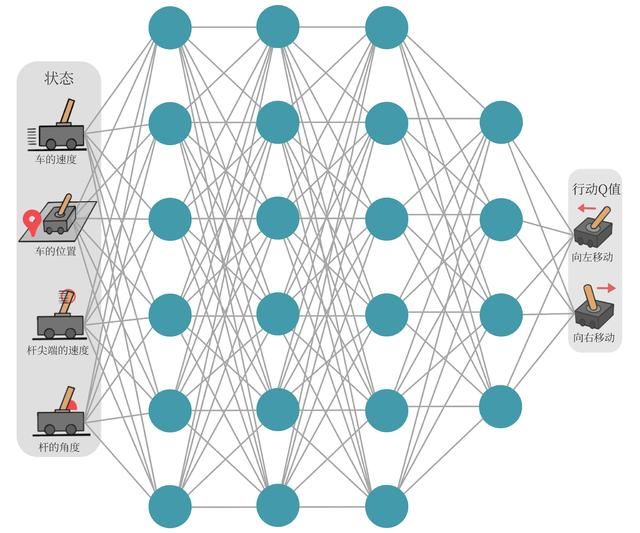
\includegraphics{images/image-0013.jpeg}
\caption{DQN 用神经网络拟合状态到各动作 Q 值的映射}
\end{figure}

\hypertarget{ux4e8cdqnux7684ux635fux5931ux51fdux6570}{%
\subsection{二、DQN的损失函数}\label{ux4e8cdqnux7684ux635fux5931ux51fdux6570}}

在传统的 Q-Learning 中，我们维护一张 \(Q\) 表。对于状态 \(s\) 和动作 \(a\)，更新规则如下：

\[
Q(s,a)\leftarrow Q(s,a)+\alpha\cdot\left[\left(r+\gamma\max_{a'}Q(s',a')\right)-Q(s,a)\right]
\]

\begin{itemize}
\tightlist
\item
  \(r+\gamma\max_{a'}Q(s',a')\) 是 TD Target（目标值），即我们认为 \(Q(s,a)\) 应该接近的值。
\item
  \(Q(s,a)\) 是 Current Estimate（当前估计值）。
\item
  物理意义：将当前的 \(Q(s,a)\) 向目标值拉近一点（步长为 \(\alpha\)）。
\end{itemize}

在 DQN 中，我们用神经网络 \(Q(s,a;\theta)\) 来拟合 \(Q\) 值。我们需要定义一个损失函数 \(L(\theta)\) 来训练网络。DQN 采用的是均方误差（MSE），目标是让网络的输出 \(Q(s,a;\theta)\) 尽可能接近 TD Target。

\[
L(\theta)=\mathbb{E}\left[\left(r+\gamma\max_{a'}Q(s',a';\theta^-)-Q(s,a;\theta)\right)^2\right]
\]

其中 \(y=r+\gamma\max_{a'}Q(s',a';\theta^-)\) 是目标值，在计算梯度时被视为常数；\(\theta^-\) 是目标网络的参数。

\hypertarget{ux4e09dqnux7684ux68afux5ea6ux66f4ux65b0}{%
\subsection{三、DQN的梯度更新}\label{ux4e09dqnux7684ux68afux5ea6ux66f4ux65b0}}

将目标值记为 \(y=r+\gamma\max_{a'}Q(s',a';\theta^-)\)，则 DQN 损失函数的梯度为：

\[
\begin{aligned}
\nabla_\theta L(\theta)
&=\nabla_\theta\left(y-Q(s,a;\theta)\right)^2\\
&=2\cdot\left(y-Q(s,a;\theta)\right)\cdot\nabla_\theta\left(-Q(s,a;\theta)\right)\\
&=-2\cdot\left[\left(r+\gamma\max_{a'}Q(s',a';\theta^-)\right)-Q(s,a;\theta)\right]\cdot\nabla_\theta Q(s,a;\theta)
\end{aligned}
\]

其中括号中的差值就是 TD Error \(\delta\)。参数更新规则（梯度下降）为：

\[
\theta\leftarrow\theta-\eta\cdot\nabla_\theta L(\theta)
\]

代入梯度后得到：

\[
\theta\leftarrow\theta+\eta\cdot2\cdot\delta\cdot\nabla_\theta Q(s,a;\theta)
\]

对比来看，Q-Learning 直接修改 \(Q(s,a)\) 的值，增加量正比于 TD Error；DQN 修改的是参数 \(\theta\)，使 \(Q(s,a;\theta)\) 的输出值沿梯度方向变化，变化幅度同样正比于 TD Error。
\#\#\# 四、经验回放

\begin{enumerate}
\def\labelenumi{\arabic{enumi}.}
\tightlist
\item
  概念
\end{enumerate}

监督学习中，我们往往假设训练数据是独立同分布的，在训练时每个batch也是随机采样的，保证了每个batch的梯度方向是对整个数据集梯度方向的一个无偏估计。但在马尔可夫决策过程（MDP）中，智能体产生的数据是一个时间序列轨迹：s\_0, a\_0, r\_0, s\_1, a\_1, r\_1,\ldots，状态s\_\{t+1\}直接依赖于s\_t和a\_t。这意味着数据高度相关，如果机器人在走迷宫，前一秒它在左下角，下一秒它大概率还在左下角附近。如果直接拿这些数据训练，神经网络会连续看到很多``左下角''的数据。数据是一个非平稳分布：随着策略pi的更新，智能体访问的状态分布也会发生变化，导致训练数据的分布本身就在变。当它极力优化当前连续片段的数据时，它会修改共享的权重，导致它``忘记''了之前在其他状态下学到的知识（和大模型推理过程中的``灾难性遗忘''亦是如此）。

因而我们引入经验回放：智能体与环境交互，每一步生成一个四元组e\_t = (s\_t, a\_t, r\_t, s\_t+1)，将这个e\_t存入固定容量的缓冲区中。在训练时刻t，我们每和环境交互一次，就从缓冲区中均匀若干次随机采样小批次的数据来进行梯度下降。

\begin{enumerate}
\def\labelenumi{\arabic{enumi}.}
\setcounter{enumi}{1}
\tightlist
\item
  优点
\end{enumerate}

打破相关性：通过随机采样，一个 batch 内的数据可能包含3天前的数据、5分钟前的数据、刚刚的数据，使得这个batch的数据分布接近于智能体的全局历史分布，而不是当前局部的一段轨迹，近似满足了独立同分布假设。

提高数据利用率：在原始Q-learning中，数据用完即弃。训练DQN网络时，每次获取新数据后，让Loss下降到接近0往往需要多次梯度下降拟合中，一个样本存入缓冲区后，可能会被多次采样用于梯度更新。这极大地提高了样本利用率（因为获取环境数据的代价通常很高）。

\begin{enumerate}
\def\labelenumi{\arabic{enumi}.}
\setcounter{enumi}{2}
\tightlist
\item
  与Dyna-Q中引入的``环境模型''的区别
\end{enumerate}

DQN不试图理解环境的运作机制，只是维护一个巨大的经验池，里面存储的是真实的元组(s\_t, a\_t, r\_t, s\_t+1)构成。每次更新参数时，从经验池中随机抽取一批曾经真实发生的数据，直接利用这些历史事实来计算损失函数并更新神经网络。

``环境模型''则维护一个函数，输入s\_t和a\_t，该函数会输出r\_t和s\_t+1。在更复杂的情境下，这个模型通常是一个神经网络。我们更新参数时，随机选择一个过去走过的(s\_t,a\_t)，但并不用过去在某一次真实发生的(r\_t,s\_t+1)，而是运用这个网络的输出值。这个函数（神经网络）具有泛化性，在高级版本中我们还可以让环境模型选择没有走过的(s\_t,a\_t)，模型可以根据学会的物理规律给出一个预测（这是经验回放做不到的，因为经验回放池里没有这一条数据），运用网络的输出值，让Q网络学习泛化性能。

\hypertarget{ux4e94ux76eeux6807ux7f51ux7edc}{%
\subsection{五、目标网络}\label{ux4e94ux76eeux6807ux7f51ux7edc}}

DQN 算法最终更新的目标是让Q(s,a)逼近r+gamma*maxQ(s',a')，由于TD误差目标本身就包含神经网络的输出，因此在更新网络参数的同时目标也在不断地改变，这非常容易造成神经网络训练的不稳定性。为了解决这一问题，DQN便使用了目标网络的思想：既然训练过程中Q网络的不断更新会导致目标不断发生改变，不如暂时先将TD目标中的Q网络固定住。为了实现这一思想，我们需要利用两套Q网络。对于损失函数：

\[
\frac{1}{2}\left[Q_w(s,a)-\left(r+\gamma\max_{a'}Q_{w^-}(s',a')\right)\right]^2
\]

原来的训练网络（主Q网络）Q\_w用于计算损失函数中的第一项，并且使用正常梯度下降方法来进行更新。目标网络Q\_w-用于计算损失函数中的第二项，其中w-表示目标网络中的参数。如果两套网络的参数随时保持一致，则仍为原先不够稳定的算法。为了让更新目标更稳定，目标网络并不会每一步都更新。具体而言，目标网络使用训练网络的一套较旧的参数，训练网络在训练中的每一步都会更新，而目标网络的参数每隔C步才会与训练网络同步一次，即。这样做使得目标网络相对于训练网络更加稳定。

当然，目标网络也不一定直接同步训练网络的值。也可以采取``软更新''：它不会大幅改动目标网络的参数，而是缓慢地将其向主Q网络的方向调整，每隔C步，计算w-\_new=τ\emph{w+(1−τ)}w-\_new。这确保了目标Q值相对稳定，为主Q网络提供了一个可靠的学习目标。

\hypertarget{ux53c2ux8003ux6587ux732e-48}{%
\subsection{参考文献}\label{ux53c2ux8003ux6587ux732e-48}}

\begin{itemize}
\tightlist
\item
  \href{https://hrl.boyuai.com/}{《动手学强化学习》}.
\item
  Mnih, V., Kavukcuoglu, K., Silver, D., et al.~(2015). \href{https://www.nature.com/articles/nature14236}{Human-level control through deep reinforcement learning}. Nature.
\end{itemize}

\clearpage

\hypertarget{double-dqn}{%
\section{Double DQN}\label{double-dqn}}

\hypertarget{ux4e00dqnux5bf9qux503cux7684ux8fc7ux9ad8ux4f30ux8ba1}{%
\subsection{一、DQN对Q值的过高估计}\label{ux4e00dqnux5bf9qux503cux7684ux8fc7ux9ad8ux4f30ux8ba1}}

DQN普遍存在过高估计Q值的问题。这是因为其更新目标为：

\[
y=r+\gamma\max_{a'}Q(s',a';w^{-})
\]

神经网络的输出Q(s',a')总是包含噪声（估计误差）。由于取max，往往最后留下的是被高估的结果，这种高估会随着贝尔曼方程的迭代不断向回传播，导致整个系统的Q值普遍虚高。假设误差epsilon服从均匀分布，我们可以推导出估计值的最大值与真实值最大值之间的期望偏差：

为了让数学推导可行，文中做了一些简化的假设，但这些假设不影响结论的普适性：

\begin{itemize}
\tightlist
\item
  \textbf{真实价值相等}：假设在状态 \(s\) 下，所有动作 \(a\) 的真实期望回报 \(Q^{*}(s,a)\) 都一样，记为 \(V^{*}(s)\)。
\item
  \textbf{为什么要这样假设}：如果真实价值本身有高有低，那么 \(\max\) 操作选到最大值是理所应当的。这里要证明的是：即使所有动作真实价值都一样，仅仅因为有噪声，\(\max\) 操作也会导致评估结果偏高。
\item
  \textbf{噪声分布}：神经网络的估算误差 \(\epsilon_a=Q_{w^{-}}(s,a)-V^{*}(s)\) 服从区间 \([-1,1]\) 上的均匀分布，且 \(\mathbb{E}[\epsilon_a]=0\)。
\item
  \textbf{独立性}：不同动作的估算误差相互独立。
\item
  \textbf{动作数量}：动作空间大小为 \(m\)。
\end{itemize}

我们的目标是计算：在这种情况下，神经网络估算出的最大值 \(\max_a Q_{w^{-}}(s,a)\) 比真实值 \(V^{*}(s)\) 高出多少，即计算期望 \(\mathbb{E}[\max_a\epsilon_a]\)。

因为 \(\epsilon_a\) 服从 \([-1,1]\) 上的均匀分布，其分布函数为：

\[
P(\epsilon_a\le x)=
\begin{cases}
0, & x\le -1\\
\frac{1+x}{2}, & x\in(-1,1)\\
1, & x\ge 1
\end{cases}
\]

现在需要求 \(m\) 个误差中的最大值 \(\max_a\epsilon_a\) 的分布。如果 \(m\) 个数的最大值都小于等于 \(x\)，那么这 \(m\) 个数每一个都必须小于等于 \(x\)。由于它们相互独立，联合概率等于各自概率的乘积：

\[
P(\max_a\epsilon_a\le x)
=\prod_{a=1}^{m}P(\epsilon_a\le x)
=(\frac{1+x}{2})^{m}
\]

最后一步是求这个``最大误差''的数学期望。期望定义为 \(\mathbb{E}[X]=\int x\cdot p(x)dx\)，其中 \(p(x)\) 是概率密度函数，也就是分布函数的导数。文中给出的积分公式为：

\[
\mathbb{E}[\max_a\epsilon_a]
=\int_{-1}^{1}x\cdot\frac{d}{dx}P(\max_a\epsilon_a\le x)dx
\]

积分结果为：

\[
=[(\frac{x+1}{2})^{m}\frac{mx-1}{m+1}]_{-1}^{1}
\]

最终得到：

\[
\mathbb{E}[\max_a Q_{w^{-}}(s,a)-\max_{a'}Q^{*}(s,a')]=\frac{m-1}{m+1}
\]

如果只有一个动作可以选择，没有max操作，那么随着每一次采样：

假设只有一个动作 \(a_1\)：

\begin{itemize}
\tightlist
\item
  \textbf{真实情况}：它的价值是 \(0\)。
\item
  \textbf{噪声}：服从 \([-1,1]\) 的均匀分布。这意味着有时会估成 \(0.8\)（高估），有时会估成 \(-0.9\)（低估）。
\end{itemize}

虽然单次看有误差，但如果尝试很多次并求平均：

\[
\mathcjk{平均误差}=\frac{(+0.8)+(-0.9)+(+0.1)+(-0.5)+\cdots}{N}\approx 0
\]

结论是：因为噪声是对称的，正向误差和负向误差会相互抵消，所以平均来看既没有过高估计，也没有过低估计，这称为无偏估计。

如果有两个动作 \(a_1\) 和 \(a_2\)，两者真实价值都是 \(0\)。Q-Learning 的 \(\max\) 操作会强迫系统挑选估值最高的那个动作。例如：

\begin{itemize}
\tightlist
\item
  第 1 次尝试：\(a_1\) 的噪声为 \(-0.5\)，\(a_2\) 的噪声为 \(+0.8\)，\(\max\) 操作选中 \(+0.8\)，结果是过高估计 \(+0.8\)。
\item
  第 2 次尝试：\(a_1\) 的噪声为 \(+0.3\)，\(a_2\) 的噪声为 \(-0.9\)，\(\max\) 操作选中 \(+0.3\)，结果是过高估计 \(+0.3\)。
\end{itemize}

动作越多，过高估计的偏差就越接近噪声的上界（这里是1）。因为动作越多，越容易每次都``运气好''碰上一个正向误差特别大的噪声，而max操作一定会选中它。

\hypertarget{ux4e8cdouble-dqn}{%
\subsection{二、Double DQN}\label{ux4e8cdouble-dqn}}

前面我们提过DQN高估Q值的问题。归根到底，这种误差来源于我们在计算目标值时，使用同一个网络（目标网络）来做两件事：选择哪个动作是最好的；评估这个动作的价值是多少。这样，每次动作都会选择高估的样本（因为高估所以选择），而每一次更新都直接运用对选择动作的价值估计（因为选择所以用于更新），导致每一次更新都写入了被高估的值。

Double DQN打破了这个链条：使用训练网络w来决定哪个动作最好，因为训练网络更新最及时，能反映最新的策略；使用目标网络w-来计算选定动作的Q值。Double DQN的更新目标变为：

\[
y_{DDQN}=r+\gamma Q(s',\arg\max_{a'}Q(s',a';w);w^{-})
\]

其中 \(\arg\max_{a'}Q(s',a';w)\) 表示由训练网络选择动作。
如果训练网络w因为噪声错误地认为某个动作最好（高估了），通过将其放入目标网络w-进行评估，由于两个网络的参数不同，w-极有可能不会同时也高估这个动作。这样就抵消了大部分的过高估计偏差。

\hypertarget{ux53c2ux8003ux6587ux732e-49}{%
\subsection{参考文献}\label{ux53c2ux8003ux6587ux732e-49}}

\begin{itemize}
\tightlist
\item
  van Hasselt, H., Guez, A., \& Silver, D. (2016). \href{https://arxiv.org/abs/1509.06461}{Deep Reinforcement Learning with Double Q-learning}. AAAI 2016.
\end{itemize}

\clearpage

\hypertarget{dueling-dqn}{%
\section{Dueling DQN}\label{dueling-dqn}}

DQN中，\(Q\) 是一个同时由状态 \(s\) 和动作 \(a\) 决定的函数。但在某些状态下，智能体只需要知道``现在的环境好不好''（\(V\) 值），而不关心具体动作的差异；而在需要通过做动作来避险或得分时，才需要关心``哪个动作比平均水平好''（\(A\) 值）。如果我们将两者分开建模，\(V(s)\) 专门负责看大局，评估当前环境好不好；\(A(s,a)\) 专门负责看细节，评估在当前环境下，哪个动作比其他动作好，好多少。这种解耦使得 \(V(s)\) 可以在每一个样本中都被学习更新（因为无论选哪个动作，\(V(s)\) 都是基础），从而大幅提升了训练效率。

\begin{figure}[htbp]
\centering
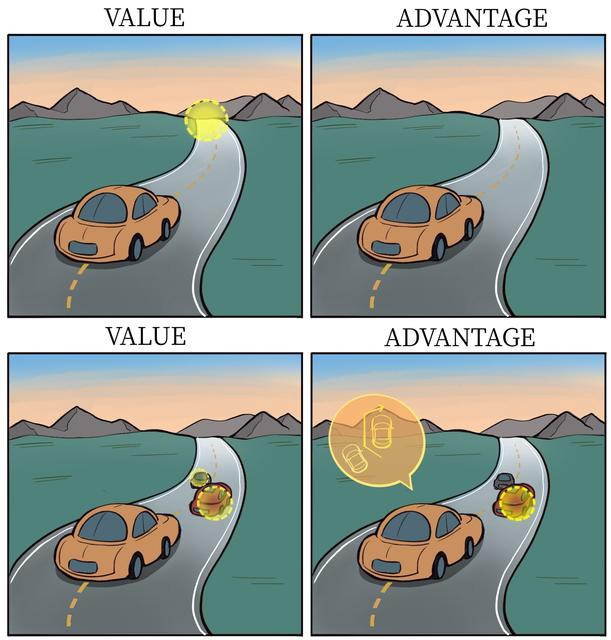
\includegraphics{images/image-0014.jpeg}
\caption{Dueling DQN 中状态价值和动作优势的直观区别}
\end{figure}

场景 A（大直道，前方无车）：此时通过屏幕（状态 \(s\)），可以判断当前局势较稳，在这个状态下大概率能得高分。此时，无论稍微向左打方向盘，还是向右打方向盘（动作 \(a\)），对最终得分的影响都较小。

\begin{itemize}
\tightlist
\item
  结论：此时 \(V(s)\)（状态价值）很高，而 \(A(s,a)\)（动作优势）的差异很小。神经网络不必费力学习每个动作的具体数值，只需要知道``这里不错''即可。
\end{itemize}

场景 B（前方有障碍物，必须急转弯）：此时状态 \(s\) 很危险，如果不操作好就会撞车。

\begin{itemize}
\tightlist
\item
  结论：此时动作选择非常重要，向左转可能存活，向右转可能失败。这时 \(A(s,a)\)（动作优势）的差异很大。
  从而我们把Q函数拆分如下：
\end{itemize}

\[
Q(s,a;\theta,\alpha,\beta)=V(s;\theta,\beta)+A(s,a;\theta,\alpha)
\]

\begin{itemize}
\tightlist
\item
  \(\theta\)：共享参数（卷积层），负责从图像中提取边缘、形状、物体位置等通用特征。这些特征既对判断局势有用，也对选择动作有用。
\item
  \(\beta\)：价值流参数（全连接层），将特征映射为一个标量 \(V\)。
\item
  \(\alpha\)：优势流参数（全连接层），将特征映射为一个向量 \(A\)，维度为动作数。
  但问题在于，我们计算和更新的都是 \(Q\) 值，怎么从 \(Q\) 值中求出 \(V\) 和 \(A\)？
\end{itemize}

我们可以获取同一个状态 \(s\) 上的所有动作 \(a'\)（遍历），各个动作 \(Q\) 值的相对大小关系也就是它们的 \(A\) 值相对大小。一个方案是对于给定 \(s\)，取让 \(Q(s,a')\) 最大的动作 \(a^*\)，设 \(A(s,a^*)=0\)（最大动作优势值），\(V(s)=Q(s,a^*)\)，则：

方案 A：Max 约束（理论最优）

\[
Q(s,a)=V(s)+(A(s,a)-\max_{a'}A(s,a'))
\]

\begin{itemize}
\tightlist
\item
  数学含义：强制让最大的优势值为 \(0\)。
  另一方案是取所有动作优势值的平均值为0：
\end{itemize}

方案 B：Mean 约束（工程最优）

\[
Q(s,a)=V(s)+(A(s,a)-\frac{1}{|\mathcal{A}|}\sum_{a'}A(s,a'))
\]

\begin{itemize}
\item
  数学含义：强制让所有动作的优势值之和为 \(0\)，也就是平均值为 \(0\)。
\item
  为什么更好：\(\max\) 操作是非线性操作，梯度只在最大值处传递，其他位置梯度为 \(0\)；而 mean 操作涉及所有动作的求和，梯度可以平滑地回传给每一个动作优势输出节点。
\item
  抗噪性：均值对异常值不那么敏感，能让网络训练更平稳。
  这样虽然不严格满足贝尔曼最优方程，但在工程实现上更优。原因如下：
\item
  数学含义：强制让所有动作的优势值之和为 \(0\)（即平均值为 \(0\)）。
\item
  为什么更好：

  \begin{itemize}
  \tightlist
  \item
    梯度稳定性：\(\max\) 操作是一个非线性操作，梯度只在最大值处传递，其他位置梯度为 \(0\)。而 mean 操作涉及所有动作的求和，梯度可以平滑地回传给每一个动作的优势输出节点。
  \item
    抗噪性：均值对异常值不那么敏感，能让网络训练更平稳。
  \end{itemize}
\end{itemize}

\hypertarget{ux53c2ux8003ux6587ux732e-50}{%
\subsection{参考文献}\label{ux53c2ux8003ux6587ux732e-50}}

\begin{itemize}
\tightlist
\item
  Wang, Z., Schaul, T., Hessel, M., van Hasselt, H., Lanctot, M., \& de Freitas, N. (2016). \href{https://arxiv.org/abs/1511.06581}{Dueling Network Architectures for Deep Reinforcement Learning}. ICML 2016.
\item
  \href{https://hrl.boyuai.com/}{《动手学强化学习》}.
\end{itemize}

\clearpage

\hypertarget{ux6709ux6a21ux578bux7684dqnux7b97ux6cd5}{%
\section{有模型的DQN算法}\label{ux6709ux6a21ux578bux7684dqnux7b97ux6cd5}}

\hypertarget{ux4e00ux7ecfux9a8cux56deux653eux65e0ux6cd5ux89e3ux51b3ux68afux5ea6ux4f20ux64adux7f13ux6162ux7684ux95eeux9898}{%
\subsection{一、经验回放无法解决梯度传播缓慢的问题}\label{ux4e00ux7ecfux9a8cux56deux653eux65e0ux6cd5ux89e3ux51b3ux68afux5ea6ux4f20ux64adux7f13ux6162ux7684ux95eeux9898}}

在标准的 Q-Learning 和 DQN 中，更新目标是：

\[
y=r+\gamma \max_{a'}Q(s',a')
\]

\begin{itemize}
\tightlist
\item
  这被称为 TD(0)。
\item
  在这个公式里，\(Q(s,a)\) 的价值更新只利用了一步之后的真实奖励 \(r\) 和下一时刻的估计 \(Q(s',a')\)。
\item
  后果：假设你在走迷宫，只有到达终点才有奖励。

  \begin{itemize}
  \tightlist
  \item
    第 1 次成功：只有终点前的最后一步状态更新了 Q 值。
  \item
    第 2 次成功：倒数第二步的状态通过倒数第一步的 Q 值更新了。
  \item
    \ldots{}
  \end{itemize}
\end{itemize}

比如说，如果我们只获得了最后一步的环境数据，没有倒数第二步的奖励值，那么在经验回放里也不会出现倒数第二步，进而梯度仍然无法通过该路径传播到前面的步骤。

经验回放（Experience Replay）相当于``翻看日记''：

\begin{itemize}
\tightlist
\item
  本质：它存储的是真实发生过的数据。
\item
  机制：你有一个数据库（Buffer），里面原封不动地记录了你在过去某个时刻做了什么、环境反馈了什么。
\item
  数据来源：真实的物理世界。
\item
  可靠性：绝对真实（Ground Truth）。只要环境本身没有发生物理规则的改变（比如摩擦力突然变了），缓冲区里的 \((s,a,r,s')\) 永远是符合物理规律的。
\item
  局限性：只能回放已经见过的场景。你无法通过回放去探索那些你从未去过的地方。
\end{itemize}

Dyna-Q 的环境模型（Environment Model）相当于``脑补模拟''：

\begin{itemize}
\tightlist
\item
  本质：它是一个被学习出来的函数（或者神经网络）。
\item
  机制：你通过观察真实数据，训练了一个模型 \(M(s,a)\to(r,s')\)。训练好后，你给它一个 \((s,a)\)，它通过计算预测出一个 \((r,s')\)。
\item
  数据来源：模型的预测（Hallucination/Prediction）。
\item
  可靠性：存在偏差（Model Bias）。如果模型没学好，它预测的结果可能是错的。例如，模型可能错误地认为``撞墙不会扣分''，基于这个错误模型的训练会导致错误的策略。
\item
  优势：泛化能力。如果使用神经网络作为模型，理论上它可以预测那些你未曾精确到达但与已知状态相似的状态的结果。
\end{itemize}

为什么说经验回放是``非参数化模型''？

在统计学中，非参数方法是指不假设数据服从某种特定分布，而是直接利用数据本身。

\begin{itemize}
\tightlist
\item
  Dyna-Q 试图学习 \(P(s'|s,a)\) 的参数（参数化）。
\item
  经验回放不学参数，直接拿样本代表分布（非参数化）。从这个角度看，经验回放就是一个不需要训练、不会产生预测偏差、但体积巨大的环境模型。
\end{itemize}

\hypertarget{ux4e8cn-step-td-learningux52a0ux901fux5df2ux83b7ux5f97ux7684ux68afux5ea6ux6570ux636eux7684ux4f20ux64ad}{%
\subsection{二、N-step TD Learning：加速已获得的梯度数据的传播}\label{ux4e8cn-step-td-learningux52a0ux901fux5df2ux83b7ux5f97ux7684ux68afux5ea6ux6570ux636eux7684ux4f20ux64ad}}

不使用环境模型，但改变目标函数的视野。DQN 可以很容易地扩展为 N-step DQN。我们不再只看一步，而是看 \(n\) 步：

\[
y=r_t+\gamma r_{t+1}+\cdots+\gamma^{n}\max_{a'}Q(s_{t+n},a')
\]

\begin{itemize}
\tightlist
\item
  作用：一次更新，奖励信号直接回传 \(n\) 步。
\item
  优缺点：比单步快，但如果 \(n\) 太大，方差（Variance）会变大。
\end{itemize}

\hypertarget{ux4e09model-based-deep-rldyna-qux7684ux771fux6b63ux7ee7ux627fux8005}{%
\subsection{三、Model-Based Deep RL：Dyna-Q的真正继承者}\label{ux4e09model-based-deep-rldyna-qux7684ux771fux6b63ux7ee7ux627fux8005}}

这才是真正对应你提到的 Dyna-Q 思想的方法。这类算法会训练一个世界模型（World Model），通常包含：

\begin{itemize}
\tightlist
\item
  动力学模型：预测 \(s_{t+1}=f(s_t,a_t)\)。
\item
  奖励模型：预测 \(r_t=R(s_t,a_t)\)。
\end{itemize}

DQN 采用经验回放，是因为在处理高维输入（如图像）时，``记住过去''比``预测未来''容易得多，也准确得多。训练一个能生成逼真游戏画面的视频生成模型（基于世界模型）比单纯训练一个玩游戏的Q网络要难得多，因此只有低维或简单环境下才会用model-based方法（如Dyna-Q）。然而，学习环境规律带来的泛化优势无可比拟，随着算力的提升和生成式AI的发展，现在的 AI 已经开始能够比较准确地``想象''未来了。因此，基于世界模型的Model-Based RL（如Dreamer算法）正在重新回归主流，试图取代或增强仅靠``回忆''（经验回放）的算法。

Dyna-Style Deep RL（如 MBPO - Model-Based Policy Optimization）：

\begin{itemize}
\tightlist
\item
  训练一个神经网络来模拟环境动力学。
\item
  在训练 Q 网络（或策略网络）时，不仅使用真实环境采样的数据（Experience Replay），还使用从模型中生成的虚拟数据。
\item
  效果：这完全复刻了 Dyna-Q 的逻辑，极大地提高了样本效率。在 MuJoCo 等控制任务上，MBPO 只需极少的真实交互就能达到很好的效果。
\end{itemize}

Latent Dynamics Models（如 Dreamer、MuZero）：

\begin{itemize}
\tightlist
\item
  Dreamer：在图像输入的任务中，先将图像编码为隐空间（Latent Space）的状态，在隐空间中学习世界模型。然后在``梦境''（隐空间的模拟序列）中训练 Actor-Critic。
\item
  MuZero：DeepMind 的算法，它不需要重构像素，而是直接在隐空间进行规划（Planning），结合了蒙特卡洛树搜索（MCTS）和模型学习。
\end{itemize}

\hypertarget{ux53c2ux8003ux6587ux732e-51}{%
\subsection{参考文献}\label{ux53c2ux8003ux6587ux732e-51}}

\begin{itemize}
\tightlist
\item
  Mnih, V., Kavukcuoglu, K., Silver, D., et al.~(2015). \href{https://doi.org/10.1038/nature14236}{Human-level control through deep reinforcement learning}. Nature.
\item
  Sutton, R. S. (1990). \href{https://doi.org/10.1016/B978-1-55860-141-3.50030-4}{Integrated Architectures for Learning, Planning, and Reacting Based on Approximating Dynamic Programming}. ICML 1990.
\item
  Janner, M., Fu, J., Zhang, M., \& Levine, S. (2019). \href{https://arxiv.org/abs/1906.08253}{When to Trust Your Model: Model-Based Policy Optimization}. NeurIPS 2019.
\item
  Hafner, D., Lillicrap, T., Ba, J., \& Norouzi, M. (2020). \href{https://openreview.net/forum?id=S1lOTC4tDS}{Dream to Control: Learning Behaviors by Latent Imagination}. ICLR 2020.
\item
  Schrittwieser, J., Antonoglou, I., Hubert, T., et al.~(2020). \href{https://doi.org/10.1038/s41586-020-03051-4}{Mastering Atari, Go, chess and shogi by planning with a learned model}. Nature.
\end{itemize}

\clearpage


% 基于策略的强化学习
\hypertarget{ux57faux4e8eux7b56ux7565ux7684ux5f3aux5316ux5b66ux4e60}{%
\chapter{基于策略的强化学习}\label{ux57faux4e8eux7b56ux7565ux7684ux5f3aux5316ux5b66ux4e60}}

\hypertarget{ux57faux4e8eux7b56ux7565ux7684ux5f3aux5316ux5b66ux4e60ux7684ux57faux672cux601dux60f3}{%
\section{基于策略的强化学习的基本思想}\label{ux57faux4e8eux7b56ux7565ux7684ux5f3aux5316ux5b66ux4e60ux7684ux57faux672cux601dux60f3}}

\hypertarget{ux4e00ux57faux4e8eux4ef7ux503cux7684ux65b9ux6cd5ux7684ux7f3aux9677}{%
\subsection{一、基于价值的方法的缺陷}\label{ux4e00ux57faux4e8eux4ef7ux503cux7684ux65b9ux6cd5ux7684ux7f3aux9677}}

基于价值的强化学习方法依赖于学习Q(s,a)，即给定状态下动作的价值函数。这意味着需要枚举所有（X个）动作以选择最优，其输出是离散的，对于连续动作（如机械臂控制），神经网络有几个输出节点，就最多只能拟合几种离散动作，导致动作僵硬；否则，拟合Q函数涉及几乎无限多个策略的期望比较、选择最优，需要的参数几乎无限多。因此，我们引入基于策略的强化学习。

\hypertarget{ux4e8cux57faux4e8eux7b56ux7565ux7684ux5f3aux5316ux5b66ux4e60}{%
\subsection{二、基于策略的强化学习}\label{ux4e8cux57faux4e8eux7b56ux7565ux7684ux5f3aux5316ux5b66ux4e60}}

\begin{enumerate}
\def\labelenumi{\arabic{enumi}.}
\tightlist
\item
  总体思想
\end{enumerate}

直接学习每个状态下的动作的概率分布，并按此分布采样动作。类似于学骑车（或者一些机器人的精密连续的动作），无法计算哪种状态价值期望最优，直接让智能体在对应状态下不断选择策略（准确说是策略的概率分布，比如也以小狗寻路为例，它会学习：在某个路口在70％左转30％右转），每次走完全程、得到累积奖励G（不同于Q函数是按最优策略计算的期望值）。我们的终极目标是找到一个策略π，使得累积奖励的期望J最大化。当策略由一个参数向量 θ（例如神经网络的权重）表示时，这个问题就转化为寻找最优的 θ。

\begin{enumerate}
\def\labelenumi{\arabic{enumi}.}
\setcounter{enumi}{1}
\tightlist
\item
  神经网络函数
\end{enumerate}

神经网络的输入为状态s，输出为动作值或动作相关参数。这个神经网络拟合了π函数，也即给定状态下动作值向量或动作相关参数的概率分布（对于连续的值，相当于概率密度函数），它是基于经验的（经验记忆在神经网络的参数θ中）。

\begin{enumerate}
\def\labelenumi{\arabic{enumi}.}
\setcounter{enumi}{2}
\tightlist
\item
  目标函数（损失函数）
\end{enumerate}

设初始状态为s0（确定），目标是让每一次完整动作链的累积奖励期望J=E\_τ\textasciitilde π(R(τ))最大，这里R(τ)表示沿着动作链τ走完全程获得的奖励，期望是按策略π对应的动作链概率分布求出的。

\begin{enumerate}
\def\labelenumi{\arabic{enumi}.}
\setcounter{enumi}{3}
\tightlist
\item
  策略梯度
\end{enumerate}

所有动作的累积奖励的期望（也就是R(τ)的期望）J对参数向量 θ的梯度：

梯度表达：我们从目标函数的定义出发，并利用期望的积分形式和对数导数技巧（Log-Likelihood Trick）进行转换。

\[
\nabla_\theta J(\theta)
=\nabla_\theta\int P(\tau|\theta)R(\tau)d\tau
=\int\nabla_\theta P(\tau|\theta)R(\tau)d\tau
\]

利用对数导数技巧 \(\nabla_\theta P(\tau|\theta)=P(\tau|\theta)\nabla_\theta\log P(\tau|\theta)\)，上式可转化为：

\[
\nabla_\theta J(\theta)
=\int P(\tau|\theta)R(\tau)\nabla_\theta\log P(\tau|\theta)d\tau
=\mathbb{E}_{\tau\sim\pi_\theta}\left[R(\tau)\nabla_\theta\log P(\tau|\theta)\right]
\]

我们将一个梯度的积分转化为了一个期望。这意味着我们可以通过采样来近似这个梯度。

我们把动作链τ分解成每一个时间步下的``元动作''：

分解轨迹概率：一条轨迹 \(\tau=(s_0,a_0,s_1,a_1,\cdots)\) 发生的概率可以分解为：

\[
P(\tau|\theta)=p(s_0)\prod_{t=0}^{T}\pi_\theta(a_t|s_t)P(s_{t+1}|s_t,a_t)
\]

其中只有策略部分 \(\pi_\theta(a_t|s_t)\) 依赖于参数 \(\theta\)。因此，当我们计算其对数梯度时，环境动态部分（初始状态分布 \(p(s_0)\) 和状态转移概率 \(P(s_{t+1}|s_t,a_t)\)）会被消去：

\[
\nabla_\theta\log P(\tau|\theta)=\sum_{t=0}^{T}\nabla_\theta\log\pi_\theta(a_t|s_t)
\]

（其中s\_i为状态，a\_i为动作，相当于(动作选择概率*状态转移概率)的累乘）

得到最终形式：将上述结果代回期望表达式，就得到了策略梯度定理的经典形式：

\[
\nabla_\theta J(\theta)
=\mathbb{E}_{\tau\sim\pi_\theta}
\left[
R(\tau)\cdot\sum_{t=0}^{T}\nabla_\theta\log\pi_\theta(a_t|s_t)
\right]
\]

\(\nabla_\theta\log\pi_\theta(a_t|s_t)\) 是什么？

\begin{itemize}
\tightlist
\item
  这是一个向量，指出了``如何在参数空间中移动，才能增加在状态 \(s_t\) 下选择动作 \(a_t\) 的概率''。
\item
  简而言之：它想让这个动作出现的概率变大。
\end{itemize}

这一项决定了梯度的方向，即θ向量梯度更新的方向。R项则决定正负、大小（对梯度向量进行缩放），正奖励越大，越促进往该方向进行梯度上升，负奖励反之。梯度值为期望，意味着我们通过按π\_θ采样即可获得无偏估计。

由于期望的下标是π\_θ，每一次的目标函数值都会随策略的变化而变化，更新策略与行为策略直接相关，这是一个在线学习算法。

\hypertarget{ux53c2ux8003ux6587ux732e-52}{%
\subsection{参考文献}\label{ux53c2ux8003ux6587ux732e-52}}

\begin{itemize}
\tightlist
\item
  Williams, R. J. (1992). \href{https://doi.org/10.1007/BF00992696}{Simple statistical gradient-following algorithms for connectionist reinforcement learning}. Machine Learning, 8, 229-256.
\item
  Sutton, R. S., McAllester, D., Singh, S., \& Mansour, Y. (1999). \href{https://proceedings.neurips.cc/paper/1999/hash/464d828b85b0bed98e80ade0a5c43b0f-Abstract.html}{Policy Gradient Methods for Reinforcement Learning with Function Approximation}. NeurIPS 1999.
\item
  Sutton, R. S., \& Barto, A. G. (2018). \href{http://incompleteideas.net/book/the-book-2nd.html}{Reinforcement Learning: An Introduction}. MIT Press.
\end{itemize}

\clearpage

\hypertarget{reinforceux7b97ux6cd5}{%
\section{REINFORCE算法}\label{reinforceux7b97ux6cd5}}

\hypertarget{ux4e00ux5956ux52b1ux9879ux7684ux53d8ux6362}{%
\subsection{一、奖励项的变换}\label{ux4e00ux5956ux52b1ux9879ux7684ux53d8ux6362}}

注意到策略梯度公式的方括号内可以视为 \(T+1\) 项相加，每一项是``\(t\) 时刻策略的对数 \(\log\pi_\theta(a_t\mid s_t)\) 对参数 \(\theta\) 的梯度，乘以该动作链全程的奖励 \(R(\tau)\)''。

\(\log\pi_\theta(a_t\mid s_t)\) 对参数 \(\theta\) 的梯度意味着``沿此方向改变 \(\theta\)，\(s_t\) 下选择 \(a_t\) 概率上升（最快）''。显然，如果该动作在未来能带来正奖励，则我们需要概率上升，否则需要减小。但是，决定梯度项大小的系数 \(R(\tau)=r_0+\cdots+r_T\) 却是从0到 \(T\) 全程的奖励，这显然不合理，在 \(t=5\) 做出的动作，不可能影响 \(t=0\) 到 \(t=4\) 已经发生的奖励。因此，和每个梯度项相乘的应该是它的未来的奖励。故把 \(R(\tau)\) 换成：

用回报 \(G_t\) 替代 \(Q\) 函数。

定理中的 \(Q^{\pi_\theta}(s_t,a_t)\) 表示在状态 \(s_t\) 采取动作 \(a_t\) 后所能获得的期望累积回报。在 REINFORCE 中，我们不知道真实的 \(Q\) 函数，但可以从采样的轨迹中计算一个实际观测到的累积回报 \(G_t\) 作为其近似值：

\[
G_t=r_t+\gamma r_{t+1}+\gamma^{2}r_{t+2}+\cdots+\gamma^{T-t}r_T
\]

这里，\(G_t\) 是 \(Q^{\pi_\theta}(s_t,a_t)\) 的一个无偏估计，但因为是单次采样结果，其方差（Variance）很高。

这时策略梯度公式变为：

\[
\nabla_\theta J(\theta)
=\mathbb{E}_{\pi_\theta}
\bigl[
\sum_{t=0}^{T}
(\sum_{t'=t}^{T}\gamma^{t'-t}r_{t'})
\nabla_\theta\log\pi_\theta(a_t|s_t)
\bigr]
\]

外层从0到 \(T\)，代表 \(\theta\) 的更新让动作链里每一个时间步的策略都得到优化；内层从 \(t\) 到 \(T\)，代表每一个优化的幅度都只取决于未来的奖励，而与 \(t\) 之前已经获得的奖励无关。

由于对于每一个给定 \(t\)、给定神经网络，上式相当于对全体 \(G_t\) 取期望，故公式也可以写成：

\[
\nabla J(\theta)
=\mathbb{E}_{\tau\sim\pi}
\bigl[
\sum_{t=0}^{T}
\nabla_\theta\log\pi_\theta(a_t|s_t)Q^{\pi}(s_t,a_t)
\bigr]
\]

这里 \(Q_\pi(s_t,a_t)\) 表示对于 \((s_t,a_t)\)，未来累积奖励 \(G_t\) 的期望值。

对于这种参数更新方式，\(\pi\) 对 \(\theta\) 的梯度表示``怎样改变参数 \(\theta\) 的值可以最快地增大在状态 \(s\) 选择动作 \(a\) 的概率 \(\pi\)''，对 \(\pi\) 取 \(\log\) 相当于沿着因变量方向``压扁''，不改变上升速度最快的（梯度）方向，但可以把 \((0,1)\) 之间的概率映射到 \((-\infty,0)\) 增大梯度值，且概率越远离1，梯度越大。当奖励 \(G_t>0\)，反向传播会倾向于增大选择 \(a\) 的概率，反之倾向于减小。

\hypertarget{ux4e8cux671fux671bux7684ux8499ux7279ux5361ux6d1bux8fd1ux4f3c}{%
\subsection{二、期望的蒙特卡洛近似}\label{ux4e8cux671fux671bux7684ux8499ux7279ux5361ux6d1bux8fd1ux4f3c}}

策略梯度定理可以直接求（所有动作按策略 \(\pi\) 给出的概率加权后）累积奖励 \(J\) 对 \(\theta\) 的梯度。但是，策略梯度定理的公式是一个期望，意味着需要对所有可能的轨迹进行加权平均，这在实际中是无法计算的。故使用蒙特卡洛方法（用频率估计概率）来近似这个期望：即通过每次运行当前一种策略，从初始到结束采样得到 \(N\) 条真实轨迹，每次运行时计算每一个 \(t\) 时刻到最终累积奖励 \(G_t\)。这等价于用 \(G_t\) 估计 \(Q_\pi(s_t,a_t)\)。

然后我们用这些轨迹作为样本，近似代替这里的期望，也就是采取类似小批量随机梯度下降的方法：每次探索一种动作路径，则：

\[
\nabla_\theta J(\theta)
\approx
\frac{1}{N}\sum_{i=1}^{N}
\bigl(
\sum_{t=0}^{T}
\nabla_\theta\log\pi_\theta(a_t^{(i)}|s_t^{(i)})G_t^{(i)}
\bigr)
\]

当然，蒙特卡洛方法估计方差较大，这主要是因为 \(G_t\) 的不稳定性。详细分析如下：

\[
\text{Gradient}\approx\nabla_\theta\log\pi_\theta(a_t|s_t)\cdot G_t
\]

项 A：\(\nabla_\theta\log\pi_\theta(a_t|s_t)\) ------ ``我们自己的部分''

这一项代表的是：``如果我想让我在状态 \(s_t\) 下做动作 \(a_t\) 的概率变大，我的参数 \(\theta\) 应该往哪个方向改？''

\begin{itemize}
\tightlist
\item
  它是确定的（Deterministic given sample）：一旦采样到了具体的 \((s_t,a_t)\)，这一项就是一个纯粹的微分计算问题。因为 \(\pi_\theta\) 是我们设计的神经网络（比如一个 MLP），其数学形式完全已知。我们通过反向传播（Backpropagation）可以精确无误地算出这个梯度向量。
\end{itemize}

项 B：\(G_t\) ------ ``环境与未来的部分''

这一项代表的是：``在这个状态 \(s_t\) 做了动作 \(a_t\) 之后，一直到游戏结束，我到底拿了多少分？''

\begin{itemize}
\tightlist
\item
  它是极度随机的（Highly Stochastic）：即使我们在完全相同的 \(s_t\) 做了完全相同的 \(a_t\)，下一次得到的 \(G_t\) 可能完全不同。因为 \(G_t\) 包含了从 \(t\) 时刻到 \(T\) 时刻所有的随机性：

  \begin{enumerate}
  \def\labelenumi{\arabic{enumi}.}
  \tightlist
  \item
    环境的随机性：也许这次风往左吹，下次风往右吹（状态转移概率 \(P(s'|s,a)\)）。
  \item
    策略的随机性：也许这次我们在 \(t+1\) 步选了动作 A，下次选了动作 B（未来策略 \(\pi\) 的随机性）。
  \end{enumerate}
\item
  它是累积的（Accumulated）：\(G_t=r_t+r_{t+1}+r_{t+2}+\cdots\)。每一个 \(r\) 都是一个随机变量。在统计学中，多个独立（或相关）随机变量之和的方差通常会随着数量线性（甚至更快）增长。如果轨迹很长，噪声会不断叠加，最后爆炸。
\end{itemize}

\hypertarget{ux4e09ux5e26ux57faux7ebfux7684reinforce}{%
\subsection{三、带基线的REINFORCE}\label{ux4e09ux5e26ux57faux7ebfux7684reinforce}}

前面的推导，我们默认奖励大于0则概率增大。但很多时候，这只会导致``所有被更新到的概率都趋于提升''，并不是我们需要的。我们需要根据动作相对于其他动作而言价值的好坏做出选择，而不是根据其绝对的价值。

虽然 REINFORCE 算法比简单策略梯度法更好，但由于我们是通过采样轨迹来估计策略梯度，这种估计往往具有较高的方差。这意味着每次采样得到的梯度值差异可能很大，这会影响算法的稳定性和收敛速度。

为了解决这个问题，我们可以引入基线（Baseline）的概念。基线的核心思想是，通过减去一个预测值来减少方差，但不改变期望值。具体来说，我们可以使用 \(G_t-b(s_t)\) 来代替 \(G_t\) 作为权重，其中 \(b(s_t)\) 是状态 \(s_t\) 的基线值。为了让期望不变，这个基线函数应该和策略函数的参数 \(\theta\) 无关。

你可以这样直观地理解：如果 \(G_t\) 大于基线 \(b(s_t)\)，则鼓励这个动作的发生；如果 \(G_t\) 小于基线 \(b(s_t)\)，则抑制这个动作的发生。

带基线的 REINFORCE 的梯度计算公式如下：

\[
\nabla_\theta J(\theta)
=\mathbb{E}_{\tau\sim\pi_\theta}
\bigl[
\sum_{t=0}^{T}
(G_t-b(s_t))\nabla_\theta\log\pi_\theta(a_t|s_t)
\bigr]
\]

这个公式与 REINFORCE 唯一的区别在于我们使用了 \(G_t-b(s_t)\) 而不是 \(G_t\)。

如果我们引入一个基线 \(b(s_t)\)，把公式变成：

\[
\nabla J(\theta)
=\mathbb{E}
\bigl[
\sum_{t=0}^{T}
\nabla\log\pi(a_t|s_t)\cdot(G_t-b(s_t))
\bigr]
\]

通常，我们把 \(b(s_t)\) 设为当前状态的平均价值（即 \(V^{\pi}(s_t)\)）。回到刚才的例子，假设平均分是 \(+55\) 分：

\begin{itemize}
\tightlist
\item
  考得烂（\(+10\)）：\(10-55=-45\)。（梯度反向，直接抑制该动作）
\item
  考得好（\(+100\)）：\(100-55=+45\)。（梯度正向，直接奖励该动作）
\end{itemize}

由于 \(b(s_t)\) 与策略参数 \(\theta\) 无关，它不影响优化过程。证明：

关键证明在于：项 \(\mathbb{E}[\sum_t \nabla_\theta \log \pi_\theta(a_t \mid s_t)\cdot b(s_t)]\) 的期望值为零。这是因为：

\[
\begin{aligned}
\mathbb{E}[\nabla_\theta \log \pi_\theta(a_t \mid s_t)b(s_t)]
&= b(s_t)\sum_a \pi_\theta(a \mid s_t)\nabla_\theta \log \pi_\theta(a \mid s_t) \\
&= b(s_t)\nabla_\theta(\sum_a \pi_\theta(a \mid s_t)) \\
&= b(s_t)\nabla_\theta 1 \\
&= 0
\end{aligned}
\]

这意味着，只要基线 \(b(s_t)\) 不依赖于动作 \(a_t\)，即它是状态的一个函数，那么它在左侧期望上就不会对梯度估计产生系统性影响，因此不会引入偏差，保持了梯度估计的无偏性。

\hypertarget{ux56dbux603bux7ed3-1}{%
\subsection{四、总结}\label{ux56dbux603bux7ed3-1}}

基于策略的强化学习算法不用枚举全部策略，比基于价值的强化学习更灵活，但可能陷入局部最优（找到一种还行的策略就不去找更好的，可通过适当增加策略初始随机性来避免）；参数稳定渐变，不会像基于价值会因为 \(Q\) 的微小变化而突变；为保证蒙特卡洛估计的准确性（\(G_t\)），相较于基于价值的强化学习，需要更大量数据。

\hypertarget{ux53c2ux8003ux6587ux732e-53}{%
\subsection{参考文献}\label{ux53c2ux8003ux6587ux732e-53}}

\begin{itemize}
\tightlist
\item
  Williams, R. J. (1992). \href{https://link.springer.com/article/10.1007/BF00992696}{Simple statistical gradient-following algorithms for connectionist reinforcement learning}. Machine Learning.
\end{itemize}

\clearpage


% 综合价值与策略的算法
\hypertarget{ux7efcux5408ux4ef7ux503cux4e0eux7b56ux7565ux7684ux7b97ux6cd5}{%
\chapter{综合价值与策略的算法}\label{ux7efcux5408ux4ef7ux503cux4e0eux7b56ux7565ux7684ux7b97ux6cd5}}

\hypertarget{actor-criticux7b97ux6cd5}{%
\section{Actor-Critic算法}\label{actor-criticux7b97ux6cd5}}

\hypertarget{ux4e00actor-criticux7b97ux6cd5ux7684ux57faux672cux539fux7406}{%
\subsection{一、Actor-Critic算法的基本原理}\label{ux4e00actor-criticux7b97ux6cd5ux7684ux57faux672cux539fux7406}}

\begin{enumerate}
\def\labelenumi{\arabic{enumi}.}
\tightlist
\item
  提出背景
\end{enumerate}

在策略梯度算法中，我们通过策略梯度获得了参数θ的调整方向，再通过动作价值的蒙特卡洛估计G\_t来获得调整的正负和幅度。但是蒙特卡洛估计存在需要样本量高、必须走完全程才能更新、方差大等问题。考虑到G\_t本身其实是对动作价值优劣的估计，我们可以结合前面基于价值的强化学习方法，引入动作价值函数。

\begin{enumerate}
\def\labelenumi{\arabic{enumi}.}
\setcounter{enumi}{1}
\tightlist
\item
  数学表示
\end{enumerate}

为了让目标函数（Q值的在状态-动作对概率分布下的期望）最大，策略梯度公式应为：

回顾我们之前得出的结论，最理想的策略梯度公式是：

\[
\nabla_\theta J(\theta)=\mathbb{E}\left[\nabla_\theta\log\pi_\theta(a\mid s)\cdot Q^\pi(s,a)\right]
\]

为了降低方差，我们通常会引入一个基线（Baseline）\(V^\pi(s)\)，将 \(Q\) 转化为优势函数（Advantage Function）：

\[
A^\pi(s,a)=Q^\pi(s,a)-V^\pi(s)
\]

这里Q(s,a)表示s状态下采取a动作的价值，V(s)表示s状态的价值，A(s,a)就是动作a相对于平均水平的优势。

根据贝尔曼方程，在一次采样中，如果接下来走到s'，则下一步更新中认为：

根据贝尔曼方程（Bellman Equation）：

\[
Q(s,a)\approx r+\gamma V(s')
\]

将这个代入优势函数公式：

\[
A(s,a)\approx \underbrace{r+\gamma V_\phi(s')-V_\phi(s)}_{\text{TD Error }\delta}
\]

从而我们并不需要构建Q网络，只需要一个V网络即可。

\begin{enumerate}
\def\labelenumi{\arabic{enumi}.}
\setcounter{enumi}{2}
\tightlist
\item
  网络更新
\end{enumerate}

和Sarsa不同：没有``Q表''

Actor-Critic算法通常由策略网络和价值网络两部分构成，将策略函数的优化与价值函数的优化分开，从而结合了两种学习的优点。

（1）策略网络（Actor）的更新

策略网络由上面的策略梯度表达式更新。我们把策略梯度中的G\_t换成了这种策略下的A(s,a)值。由于我们不需要G\_t，而是可以直接利用价值网络存储的A(s,a)，故每走一步，就可以进行一次更新。当A(s,a)＞0时，会倾向于让a的概率增大，反之倾向于减小。

（2）价值网络（Critic）的更新

当从状态s到s'，获得奖励r，V(s)的更新目标Target=r+gamma*V(s')。

\begin{enumerate}
\def\labelenumi{\arabic{enumi}.}
\setcounter{enumi}{3}
\tightlist
\item
  与其他算法（Sarsa、DQN）的对比
\end{enumerate}

（1）与Sarsa的对比

Sarsa的Q既负责打分，也负责决策（epsilon-greedy策略），而Critic的Q只负责打分，策略权在Actor手里；Sarsa有显式Q表，Critic通过深度学习拟合。

相同点（The Core DNA）：

\begin{itemize}
\tightlist
\item
  数学根据一致：都基于贝尔曼期望方程（Bellman Expectation Equation），即 \(\mathrm{Value}\approx r+\gamma\cdot\mathrm{Next\_Value}\)。这里的 \(\mathrm{Next\_Value}\) 都是指``按照当前策略走下去的价值''，不取最大值。
\item
  策略属性一致：通常都是 On-policy（同策略）。它们更新的目标值，紧紧跟随当前智能体的实际行为模式；如果智能体变笨了，它们评估出的价值也会变低。
\end{itemize}

\begin{longtable}[]{@{}
  >{\raggedright\arraybackslash}p{(\columnwidth - 4\tabcolsep) * \real{0.33}}
  >{\raggedright\arraybackslash}p{(\columnwidth - 4\tabcolsep) * \real{0.33}}
  >{\raggedright\arraybackslash}p{(\columnwidth - 4\tabcolsep) * \real{0.33}}@{}}
\toprule
维度 & Critic（通常指 V-based） & Sarsa（Q-based） \\
\midrule
\endhead
所需数据 & \(S,A,R,S'\) & \(S,A,R,S',A'\) \\
更新时机 & 看到状态 \(S'\) 即可更新。它只需要预估 \(S'\) 的平均前景。 & 必须等到选出 \(A'\) 后。它必须知道下一步确切走了哪条路。 \\
更新目标 & \(Target=r+\gamma V(s')\)，直接使用状态价值，隐含了对动作的期望。 & \(Target=r+\gamma Q(s',a')\)，使用下一步实际发生动作的价值。 \\
随机性/方差 & 较低。\(V(s')\) 是网络输出的平滑值，过滤掉了下一步选动作的随机噪声。 & 较高。受下一步动作 \(a'\) 的具体选择影响，可能这步走得很好、下步走得烂，导致 Target 波动。 \\
核心角色 & 辅助者（Coach）。它只负责打分，必须配合 Actor 使用，自己不产出动作。 & 独裁者（Doer）。既负责打分，又直接根据分值决定动作（\(\epsilon\)-greedy）。 \\
\bottomrule
\end{longtable}

（2）与DQN的对比

Critic和Sarsa运用的都是贝尔曼期望方程，而DQN运用的是贝尔曼最优方程。Critic和Sarsa根据当前策略对应的概率分布，估计价值的期望，数据必须实时由当前策略生成，具体体现：

Sarsa：

\[
Q(s,a)\leftarrow Q(s,a)+\alpha\left[\underbrace{r+\gamma Q(s',a')}_{\text{Target}}-Q(s,a)\right]
\]

Critic：

\[
L=\left(\underbrace{r+\gamma V(s')}_{\text{Target}}-V(s)\right)^2
\]

虽然式子里看起来没有策略，但是这种更新方式意味着V(s)本质上是过去不同动作得到的Q(s,a)（即r+gamma*V(s')）的移动平均。随着策略的变化，不同动作的概率分布也就会变化，因此在下一步，必须重新根据此刻的策略（动作概率分布）采样新的动作a，才能保证r+V(s')的期望是对新的策略的价值的无偏估计，而不能用别的策略下采样的动作进行V的更新，因而它是On-policy的。

而DQN的更新与策略无关，只取最优价值。

\begin{longtable}[]{@{}llll@{}}
\toprule
特性 & Critic（in AC） & Sarsa & DQN \\
\midrule
\endhead
核心方程 & 贝尔曼期望方程 & 贝尔曼期望方程 & 贝尔曼最优方程 \\
目标值（Target） & \(r+\gamma V(s')\) & \(r+\gamma Q(s',a')\) & \(r+\gamma\max Q(s',a')\) \\
对未来的态度 & 诚实（基于当前概率） & 诚实（基于实际选择） & 乐观（假设未来最优） \\
所需样本 & \((s,a,r,s')\) & \((s,a,r,s',a')\) & \((s,a,r,s')\) \\
数据利用 & On-policy（通常不复用） & On-policy（通常不复用） & Off-policy（可复用经验池） \\
主要用途 & 减小 PG 的方差（PPO/A2C） & 学习安全保守的策略 & 学习寻找最优解的策略 \\
\bottomrule
\end{longtable}

场景：一条路紧贴着悬崖。掉下去扣 100 分，走正路扣 1 分。

策略特点：现在的策略 \(\pi\) 还有点笨，有 \(10\%\) 的概率会手滑掉下去（\(\epsilon\)-greedy）。

DQN（Q-Learning）的视角：

\begin{itemize}
\tightlist
\item
  它会说：``嘿，贴着悬崖走是最短路径！只要我不手滑（取 max），这就是最优解。''
\item
  结果：它学出的价值函数会鼓励你贴着悬崖走。但因为你实际上会手滑，你就会不断掉下去。
\item
  特点：盲目自信，评估的是``理论上的完美策略''。
\end{itemize}

SARSA（以及 AC 中的 Critic）的视角：

\begin{itemize}
\tightlist
\item
  它会说：``嘿，虽然贴着悬崖走最近，但以你现在的笨拙程度（当前策略 \(\pi\)），你走那条路有很大几率掉下去摔死。所以那条路的价值（\(Q\) 或 \(V\)）其实很低！''
\item
  结果：它给出的价值估计会逼迫 Actor 离悬崖远一点，走安全的路。
\item
  特点：实事求是，评估的是``你现在的真实水平''。
\end{itemize}

\begin{enumerate}
\def\labelenumi{\arabic{enumi}.}
\setcounter{enumi}{4}
\tightlist
\item
  训练和前向推理时的组件
\end{enumerate}

所有存在Actor和Critic的模型架构，包括后面介绍的TRPO、PPO、DDPG、SAC等，都遵循以下原则：

训练时：Actor和Critic同时工作。

前向推理时：舍弃Critic，只留Actor。

这就好比你学开车（训练）时，教练（Critic）坐在副驾不停地给你打分、纠正动作（更新策略）；但是当你拿到驾照自己上路（推理）时，教练就不在了，只有你（Actor）在开车，你只需要看路况（状态）并打方向盘（动作），动作也不需要再纠正（策略不再更新）。

\hypertarget{ux4e8ca2cux548ca3c}{%
\subsection{二、A2C和A3C}\label{ux4e8ca2cux548ca3c}}

由前面介绍的内容，这是一个On-Policy算法，而且无法像SAC那样建立Replay Buffer（原因见SAC部分），每次更新策略都必须重新采样。这不仅不适合并行计算，而且导致了严重的数据相关性问题，因为相近时刻的状态s也比较相近，随着训练进行，状态随时间的分布会改变，数据不满足独立同分布假设。故我们需要有不同Worker在同一时刻分别采样，统一更新梯度。具体有以下两种底层实现方法。

\begin{enumerate}
\def\labelenumi{\arabic{enumi}.}
\tightlist
\item
  A3C（Google DeepMind,ICML 2016）
\end{enumerate}

每一个Worker都是一个独立的进程，进程里都有一个环境副本、一个本地神经网络副本。Worker自己在本地网络跑前向传播，算出梯度，然后把梯度推送到全局网络，并把全局网络的最新参数拉回来覆盖本地网络。

\begin{enumerate}
\def\labelenumi{\arabic{enumi}.}
\setcounter{enumi}{1}
\tightlist
\item
  A2C（OpenAI,2017）
\end{enumerate}

使用multiprocessing也就是所谓的SubprocVecEnv（子进程向量化环境）。每一个Worker进程里只有一个环境副本，主进程持有唯一的一个神经网络（通常在GPU上）。16个Worker并行执行env.step()，返回各自状态。主进程收集16个s，拼接成一个Batch，用GPU一次性算出16个各自的动作，发回给Worker。Worker非常轻量，只负责模拟物理环境。

目前主流的Actor-Critic算法（包括PPO），其底层并行架构基本都沿用了A2C的``向量化环境''模式。

\hypertarget{ux53c2ux8003ux6587ux732e-54}{%
\subsection{参考文献}\label{ux53c2ux8003ux6587ux732e-54}}

\begin{itemize}
\tightlist
\item
  Mnih, V., Badia, A. P., Mirza, M., et al.~(2016). \href{https://arxiv.org/abs/1602.01783}{Asynchronous Methods for Deep Reinforcement Learning}. ICML 2016.
\item
  OpenAI. (2017). \href{https://openai.com/index/openai-baselines-acktr-a2c/}{OpenAI Baselines: ACKTR \& A2C}.
\end{itemize}

\clearpage

\hypertarget{trpoux7b97ux6cd5ux4e0eux91cdux8981ux6027ux91c7ux6837}{%
\section{TRPO算法与重要性采样}\label{trpoux7b97ux6cd5ux4e0eux91cdux8981ux6027ux91c7ux6837}}

\hypertarget{ux4e00ux63d0ux51faux80ccux666f}{%
\subsection{一、提出背景}\label{ux4e00ux63d0ux51faux80ccux666f}}

在强化学习中，尤其是在策略梯度方法中，我们通过不断更新策略网络（一个概率分布）来让智能体表现得更好。但这里有一个巨大的风险：如果一次更新步子迈得太大，新策略可能会彻底``跑偏''，选择一个很差的动作，进而采样到差的数据，算出不准的梯度，恶性循环，导致训练崩溃、性能急剧下降，并且很难恢复。

\hypertarget{ux4e8cux6570ux5b66ux8868ux8fbe-1}{%
\subsection{二、数学表达}\label{ux4e8cux6570ux5b66ux8868ux8fbe-1}}

在机器学习中，KL散度 \(D_{\mathrm{KL}}(P\Vert Q)=H(P,Q)-H(P)\) 可以表示预测分布 \(Q\) 和标签分布 \(P\) 之间的差异，这里 \(H(P,Q)\) 是交叉熵，即用 \(Q\) 的编码系统去编码 \(P\) 的数据所需的平均长度。准确地说，这是前向KL散度，衡量了使用了错误的编码系统（\(Q\)）而导致与正确编码系统（\(P\)）相比额外多出的信息量，也就是 \(Q\) 偏离 \(P\) 的程度，在旧策略 \(P\) 概率高而新策略 \(Q\) 概率低的时候，惩罚会很大，这保证了新策略覆盖原策略，不会过度收缩（Collapse），避免忽略了真实分布的某些模式。还有一种KL散度是反向KL散度，即 \(D_{\mathrm{KL}}(Q\Vert P)\)，它在旧策略 \(P\) 概率低而新策略 \(Q\) 概率高的时候，惩罚很大。

将KL散度运用到强化学习中，则是像一个~``稳定器''或``刹车''~。大模型一般均用反向KL散度），因为反向KL散度会对新策略高概率、原策略低概率的区域给出较大惩罚，进而让新的概率空间不跳出预训练后概率较大的空间（如果跳出空间往往表现为输出乱码、不符合正常语义的内容等，即``模式崩塌''）。RL获得的空间往往是预训练的子集（这也可能是RL难以让模型获得预训练完全没见过的技能的原因之一）。

我们知道，KL散度 \(D_{\mathrm{KL}}(P\Vert Q)=H(P,Q)-H(P)\)，其中 \(H(P,Q)\) 为交叉熵。在 TRPO 或 PPO 这类算法中，我们为什么用KL散度而不用交叉熵呢？不是因为梯度不同（它们梯度其实一样），而是因为``标尺''的零点不同。KL散度提供了一个绝对的零点（即 \(D_{\mathrm{KL}}=0\) 代表没变化），这让我们能设定一个通用的安全阈值（Trust Region）；而交叉熵的``零点''是浮动的（等于旧策略的熵 \(H(P)\)），导致无法设定一个固定的阈值来限制更新幅度。

TRPO算法可以表达为这样一个优化问题：

\[
\begin{aligned}
\max_\theta\quad
& \mathbb{E}_{s\sim\rho_{\theta_{\mathrm{old}}},\,a\sim\pi_{\theta_{\mathrm{old}}}}
\bigl[
\frac{\pi_\theta(a\mid s)}{\pi_{\theta_{\mathrm{old}}}(a\mid s)}
A^{\pi_{\mathrm{old}}}(s,a)
\bigr] \\
\text{subject to}\quad
& \bar{D}_{\mathrm{KL}}(\pi_{\theta_{\mathrm{old}}}\Vert \pi_\theta)\le \delta
\end{aligned}
\]

其中 \(\frac{\pi_\theta(a\mid s)}{\pi_{\theta_{\mathrm{old}}}(a\mid s)}\) 是概率比率，\(A^{\pi_{\mathrm{old}}}(s,a)\) 是优势函数，\(\delta\) 是信赖域半径，也就是允许策略变动的最大幅度。

\hypertarget{ux4e09ux76eeux6807ux51fdux6570ux91cdux8981ux6027ux91c7ux6837ux7684ux89e3ux91ca}{%
\subsection{三、目标函数（重要性采样）的解释}\label{ux4e09ux76eeux6807ux51fdux6570ux91cdux8981ux6027ux91c7ux6837ux7684ux89e3ux91ca}}

TRPO是一个Online Policy，随着策略的更新，从旧策略中采样的数据就无法使用，造成了极大的数据浪费。为了能有效利用旧数据，我们采取了统计学中重要性采样的方法。

假设你的任务是统计全国人民的平均收入。

\begin{itemize}
\tightlist
\item
  目标分布 \(P\)（Target）：全国人民的分布。
\item
  采样分布 \(Q\)（Proposal）：你作为采样员，只能在上海陆家嘴街头随机拉人问收入。
\end{itemize}

直接算平均值的问题：如果你直接拿陆家嘴路人的平均收入，结果肯定远高于全国平均水平，因为你采样的地点（分布 \(Q\)）偏向富人。

重要性采样的解决方案：你可以继续在陆家嘴采样，但算账时要加权重：

\begin{enumerate}
\def\labelenumi{\arabic{enumi}.}
\tightlist
\item
  富人：在陆家嘴很多，但在全国比例没那么高，给他们的收入乘一个小于 \(1\) 的权重（降权）。
\item
  普通收入者：在陆家嘴很少，但在全国比例很高；如果你在陆家嘴好不容易遇到一个普通人，这个样本就太珍贵了，它代表了全国那一大群人，给他的收入乘一个大于 \(1\) 的权重（加权）。
\end{enumerate}

假设我们需要计算某个函数 \(f(x)\) 在目标分布 \(P(x)\) 下的期望，但只能从另一个分布 \(Q(x)\) 采样：

\[
\mathbb{E}_{x\sim P}[f(x)] = \int P(x)f(x)\,dx
\]

做恒等变换：

\[
\begin{aligned}
\mathbb{E}_{x\sim P}[f(x)]
&= \int P(x)f(x)\cdot \frac{Q(x)}{Q(x)}\,dx \\
&= \int Q(x)(\frac{P(x)}{Q(x)}f(x))\,dx
\end{aligned}
\]

因此：

\[
\mathbb{E}_{x\sim P}[f(x)]
=
\mathbb{E}_{x\sim Q}
\bigl[
\frac{P(x)}{Q(x)}f(x)
\bigr]
\]

其中 \(\frac{P(x)}{Q(x)}\) 就是重要性权重（Importance Weight）。

这样，我们就能对旧策略Q采样出来的数据进行``再利用''了。

应用在TRPO中，即：

\[
\mathbb{E}_{a\sim\pi_{\mathrm{old}}}
\bigl[
\frac{\pi_{\mathrm{new}}(a\mid s)}{\pi_{\mathrm{old}}(a\mid s)}
A(s,a)
\bigr]
\]

当然，这个公式是在s给定的条件下的期望，还没有考虑s的占用度量会随着策略变化而变化。考虑后，公式如下：

\[
J(\theta)=
\sum_s\rho_{\pi_\theta}(s)
\sum_a\pi_\theta(a\mid s)r(s,a)
\]

利用重要性采样变换后：

\[
J(\theta)=
\mathbb{E}_{s\sim\rho_{\theta_{\mathrm{old}}},\,a\sim\pi_{\theta_{\mathrm{old}}}}
\bigl[
\frac{\rho_{\pi_\theta}(s)}{\rho_{\pi_{\theta_{\mathrm{old}}}}(s)}
\cdot
\frac{\pi_\theta(a\mid s)}{\pi_{\theta_{\mathrm{old}}}(a\mid s)}
\cdot
A^{\pi_{\mathrm{old}}}(s,a)
\bigr]
\]

困难点在于：计算 \(\frac{\rho_{\pi_\theta}(s)}{\rho_{\pi_{\theta_{\mathrm{old}}}}(s)}\) 是极其困难的。\(\rho(s)\) 这种状态占用分布由环境动力学 \(P(s'\mid s,a)\) 和策略 \(\pi\) 经过多步交互共同决定，不像动作概率 \(\pi(a\mid s)\) 那样可以直接从策略网络读出来。除非你知道环境的完整模型并解复杂的流方程，否则很难显式求出这个状态分布比值。

TRPO 的做法是直接近似令：

\[
\frac{\rho_{\pi_\theta}(s)}{\rho_{\pi_{\theta_{\mathrm{old}}}}(s)}\approx 1
\]

也就是说，它假设在我更新策略的一瞬间，遇到的状态分布还没来得及发生剧烈变化。

我们可以看到，重要性采样必须以限制Q相对于P的偏差为前提。否则，就好比你在陆家嘴（Q）好不容易抓到一个极度罕见的贫困户，根据公式，这个人的样本权重会变成几万倍，这一个样本就会主导整个梯度的计算，导致神经网络的更新方向剧烈波动，模型直接训练崩溃。

\hypertarget{ux56dbux4f18ux5316ux95eeux9898ux7684ux6c42ux89e3}{%
\subsection{四、优化问题的求解}\label{ux56dbux4f18ux5316ux95eeux9898ux7684ux6c42ux89e3}}

TPRO可以被写成下面的优化问题：

\[
\begin{aligned}
\max_\theta\quad
& L(\theta)=\mathbb{E}
\bigl[
\frac{\pi_\theta}{\pi_{\mathrm{old}}}A
\bigr] \\
\text{subject to}\quad
& \bar{D}_{\mathrm{KL}}(
\pi_{\theta_{\mathrm{old}}}(\cdot\mid s)
\Vert
\pi_\theta(\cdot\mid s)
)\le \delta
\end{aligned}
\]

求解如下：

第一步：泰勒展开（近似化）

令：

\[
x=\theta-\theta_{\mathrm{old}}
\]

由于信赖域很小，可以对目标函数和约束进行泰勒展开。

\begin{enumerate}
\def\labelenumi{\arabic{enumi}.}
\tightlist
\item
  对目标函数 \(L(\theta)\) 做一阶展开：
\end{enumerate}

\[
L(\theta)\approx
L(\theta_{\mathrm{old}})
+
\nabla_\theta L(\theta_{\mathrm{old}})^{T}x
\]

其中 \(L(\theta_{\mathrm{old}})\) 是常数，不影响优化；\(\nabla_\theta L(\theta_{\mathrm{old}})\) 就是标准的策略梯度，记为向量 \(\mathbf{g}\)。因此近似目标变为：

\[
\max_x\ \mathbf{g}^{T}x
\]

\begin{enumerate}
\def\labelenumi{\arabic{enumi}.}
\setcounter{enumi}{1}
\tightlist
\item
  对约束条件 \(\bar{D}_{\mathrm{KL}}\) 做二阶展开：
\end{enumerate}

\[
\bar{D}_{\mathrm{KL}}\bigl(
\pi_{\theta_{\mathrm{old}}}(\cdot\mid s)
\Vert
\pi_{\theta_{\mathrm{old}}+x}(\cdot\mid s)
\bigr)
\approx
\bar{D}_{\mathrm{KL}}\bigl(
\pi_{\theta_{\mathrm{old}}}(\cdot\mid s)
\Vert
\pi_{\theta_{\mathrm{old}}}(\cdot\mid s)
\bigr)
+
(\nabla_\theta \bar{D}_{\mathrm{KL}})^{T} x
+
\frac{1}{2}x^{T}\nabla_\theta^{2}\bar{D}_{\mathrm{KL}}x
\]

第一项 \(\bar{D}_{\mathrm{KL}}(\pi_{\theta_{\mathrm{old}}}(\cdot\mid s)\Vert\pi_{\theta_{\mathrm{old}}}(\cdot\mid s))=0\)；第二项在新旧策略分布相等时取极小值，导数为 \(0\)。第三项中的 \(\nabla_\theta^{2}\bar{D}_{\mathrm{KL}}\) 是 KL 散度的二阶导数矩阵，也就是费雪信息矩阵（Fisher Information Matrix, FIM），记为 \(\mathbf{H}\)。因此约束近似为：

\[
\frac{1}{2}x^{T}\mathbf{H}x\le \delta
\]

第二步：求解新方向（拉格朗日乘子法）

现在问题变为：

\[
\begin{aligned}
\max_x\quad
& \mathbf{g}^{T}x \\
\text{subject to}\quad
& \frac{1}{2}x^{T}\mathbf{H}x\le \delta
\end{aligned}
\]

构建拉格朗日函数：

\[
\mathcal{L}(x,\lambda)=
\mathbf{g}^{T}x
-\lambda
\bigl(
\frac{1}{2}x^{T}\mathbf{H}x-\delta
\bigr)
\]

对 \(x\) 求导并令导数为 \(0\)：

\[
\mathbf{g}-\lambda\mathbf{H}x=0
\quad\Longrightarrow\quad
\mathbf{H}x=\frac{1}{\lambda}\mathbf{g}
\]

于是我们得到了更新方向（还没有确定步长）：

\[
x\propto\mathbf{H}^{-1}\mathbf{g}
\]

这就是著名的自然梯度（Natural Gradient）方向。它不是沿着普通梯度 \(\mathbf{g}\) 走，而是用曲率矩阵 \(\mathbf{H}\) 的逆去修正方向。

接下来确定步长（缩放系数）。将：

\[
x=\beta\mathbf{H}^{-1}\mathbf{g}
\]

代入约束条件 \(\frac{1}{2}x^{T}\mathbf{H}x=\delta\)，得到：

\[
\beta=
\sqrt{
\frac{2\delta}{\mathbf{g}^{T}\mathbf{H}^{-1}\mathbf{g}}
}
\]

最终的参数更新公式为：

\[
x^{*}
=
\sqrt{
\frac{2\delta}{\mathbf{g}^{T}\mathbf{H}^{-1}\mathbf{g}}
}
\mathbf{H}^{-1}\mathbf{g}
\]

第三步：数值求解（共轭梯度法 CG）

虽然公式推出来了，但工程上根本没法直接算。痛点在于 \(\mathbf{H}\) 是 Hessian 矩阵，维度是 \(N\times N\)（\(N\) 是参数量）。如果参数有 100 万，\(\mathbf{H}\) 就有 1 万亿个元素，内存直接爆炸，更别提求逆矩阵 \(\mathbf{H}^{-1}\) 了。

TRPO 的核心魔法是共轭梯度法（Conjugate Gradient, CG）。我们需要计算的是向量：

\[
\mathbf{s}=\mathbf{H}^{-1}\mathbf{g}
\]

等价于求解线性方程组：

\[
\mathbf{H}\mathbf{s}=\mathbf{g}
\]

CG 算法的特点是：求解 \(\mathbf{H}\mathbf{s}=\mathbf{g}\) 不需要显式地写出矩阵 \(\mathbf{H}\)，只需要能够计算矩阵-向量乘积 \(\mathbf{H}v\)。也就是说，只要你能给我一个函数，输入向量 \(v\)，输出 \(\mathbf{H}v\)，我就能迭代解出 \(\mathbf{s}\)。

\(\mathbf{H}\) 是 KL 散度的二阶导数。计算 \(\mathbf{H}v\) 不需要真的算二阶导，有一个极其高效的技巧（Pearlmutter Trick）：

\[
\mathbf{H}v
=
\nabla_\theta(\nabla_\theta D_{\mathrm{KL}}\cdot v)
\]

具体做法是：

\begin{enumerate}
\def\labelenumi{\arabic{enumi}.}
\tightlist
\item
  先算 KL 散度的梯度 \(\nabla_\theta D_{\mathrm{KL}}\)。
\item
  算这个梯度和向量 \(v\) 的点积，得到一个标量。
\item
  再对这个标量求一次梯度。
\end{enumerate}

在 PyTorch / TensorFlow 这类自动微分框架下，这只需要做两次反向传播，速度很快，且不需要存储矩阵。

第四步：线性搜索（Line Search）

前面的二阶近似只是近似。真正更新后，实际 KL 散度可能会超过 \(\delta\)，或者真实目标函数反而下降。为了保证万无一失，TRPO 最后会做回溯线性搜索（Backtracking Line Search）：

\begin{enumerate}
\def\labelenumi{\arabic{enumi}.}
\tightlist
\item
  算出理想更新量 \(x^{*}\)。
\item
  设实际更新量：
\end{enumerate}

\[
\Delta\theta=\alpha^{j} x^{*}
\quad
(\alpha \mathcjk{ \mathcjk{初始为} } 1)
\]

\begin{enumerate}
\def\labelenumi{\arabic{enumi}.}
\setcounter{enumi}{2}
\tightlist
\item
  检查两个条件：
\end{enumerate}

\[
\bar{D}_{\mathrm{KL}}(
\pi_{\theta_{\mathrm{old}}}(\cdot\mid s)
\Vert
\pi_{\theta_{\mathrm{old}}+\Delta\theta}(\cdot\mid s)
)\le \delta
\]

\[
L(\theta_{\mathrm{old}}+\Delta\theta)\ge L(\theta_{\mathrm{old}})
\]

\begin{enumerate}
\def\labelenumi{\arabic{enumi}.}
\setcounter{enumi}{3}
\tightlist
\item
  如果不行，就让 \(j\leftarrow j+1\)，比如 \(\alpha\) 变成 \(0.5,0.25,\ldots\)，缩短步长再试。
\item
  直到满足条件，才真正更新参数。
\end{enumerate}

总结 TRPO 的求解流程：

\begin{enumerate}
\def\labelenumi{\arabic{enumi}.}
\tightlist
\item
  准备数据：用旧策略收集一批轨迹。
\item
  算梯度：计算策略梯度 \(\mathbf{g}\)。
\item
  算方向（CG）：利用 Hessian-向量积技巧，跑若干步共轭梯度算法，解出 \(\mathbf{s}\approx\mathbf{H}^{-1}\mathbf{g}\)。
\item
  算系数：代入公式算出最大步长系数 \(\beta\)。
\item
  线性搜索：沿着 \(\beta\mathbf{s}\) 方向试探，找到满足约束的最大步长。
\item
  更新：\(\theta_{\mathrm{new}}=\theta_{\mathrm{old}}+\mathrm{final\_step}\)。
\end{enumerate}

\hypertarget{ux53c2ux8003ux6587ux732e-55}{%
\subsection{参考文献}\label{ux53c2ux8003ux6587ux732e-55}}

\begin{itemize}
\tightlist
\item
  Schulman, J., Levine, S., Abbeel, P., Jordan, M., \& Moritz, P. (2015). \href{https://arxiv.org/abs/1502.05477}{Trust Region Policy Optimization}. ICML 2015.
\end{itemize}

\clearpage

\hypertarget{ppoux7b97ux6cd5ux4e0egae}{%
\section{PPO算法与GAE}\label{ppoux7b97ux6cd5ux4e0egae}}

PPO由TRPO衍生而来。TRPO提出了运用重要性采样、限制更新范围等，但它作为一个带约束的优化问题，求解十分复杂，是一个``精确但昂贵''的算法，在大模型中并不实用。我们想到，可以将约束条件直接写入目标函数。具体而言，有两种方法，也因此产生了PPO的两种变体。

\hypertarget{ux4e00ppo-penalty}{%
\subsection{一、PPO-Penalty}\label{ux4e00ppo-penalty}}

目标函数如下：

\[
J^{\mathrm{PEN}}(\theta)
=
\mathbb{E}_t
\bigl[
\frac{\pi_\theta(a_t\mid s_t)}
{\pi_{\theta_{\mathrm{old}}}(a_t\mid s_t)}
A_t
-
\beta\cdot
D_{\mathrm{KL}}
\bigl(
\pi_{\theta_{\mathrm{old}}}(\cdot\mid s_t)
\Vert
\pi_\theta(\cdot\mid s_t)
\bigr)
\bigr]
\]

\begin{itemize}
\tightlist
\item
  第一项：TRPO 中的代理目标，即 Ratio \(\times\) Advantage，负责让策略变好。
\item
  第二项：KL 散度惩罚项，\(D_{\mathrm{KL}}\) 衡量新旧策略分布的差异。
\item
  \(\beta\)：惩罚系数。\(\beta\) 越大，越不允许策略剧烈变化。
\end{itemize}

这里第一项同TRPO，即找到一个新策略，让获得奖励在新策略下的期望最大；第二项的前向KL散度主要意在确保旧策略 \(\pi_{\mathrm{old}}\) 概率高的区域，如预训练中学习到的常见的人类语言模式和世界基础知识，新策略 \(\pi_{\mathrm{new}}\) 概率也高，避免模型为了获取更高的 Reward 而丢弃预训练中学习到的知识而发生``模式崩塌''；而对于一些旧策略概率较低的高难度问题解法，新策略在提高概率的同时不会受到过度的惩罚。这样可以保证每次更新都在一个可信的``信任区域''内进行。

PPO-Penalty 的精髓在于它不是使用固定的 \(\beta\)，而是根据每一轮更新后的实际 KL 散度值动态调整。设：

\[
d = D_{\mathrm{KL}}(\pi_{\mathrm{old}},\pi_{\mathrm{new}})
\]

设定一个目标 KL 值 \(d_{\mathrm{targ}}\)，例如 \(0.01\)：

\begin{enumerate}
\def\labelenumi{\arabic{enumi}.}
\tightlist
\item
  如果 \(d < d_{\mathrm{targ}}/1.5\)，说明策略变动太小、过于保守，于是减小 \(\beta\)，例如：
\end{enumerate}

\[
\beta \leftarrow \beta/2
\]

让下一轮步子迈大一点。

\begin{enumerate}
\def\labelenumi{\arabic{enumi}.}
\setcounter{enumi}{1}
\tightlist
\item
  如果 \(d > d_{\mathrm{targ}}\times 1.5\)，说明策略变动太大、过于激进，于是增大 \(\beta\)，例如：
\end{enumerate}

\[
\beta \leftarrow 2\beta
\]

让下一轮受到的惩罚更重。

\hypertarget{ux4e8cppo-clipux4e3bux6d41}{%
\subsection{二、PPO-Clip（主流）}\label{ux4e8cppo-clipux4e3bux6d41}}

\[
r_t(\theta)=
\frac{\pi_\theta(a_t\mid s_t)}
{\pi_{\theta_{\mathrm{old}}}(a_t\mid s_t)}
\]

\[
J^{\mathrm{CLIP}}(\theta)
=
\mathbb{E}_t
\bigl[
\min\bigl(
r_t(\theta)A_t,\,
\mathrm{clip}(r_t(\theta),1-\epsilon,1+\epsilon)A_t
\bigr)
\bigr]
\]

上式中 \(A_t\) 表示动作的相对价值（下面会讲），我们希望新策略能让价值在该策略下的期望最大，经重要性采样可得上式，\(J\) 对 \(\theta\) 的导数即为此时参数网络更新的梯度。\(A_t\) 大于 \(0\) 时，我们会希望 \(\pi_\theta\) 更大，这等价于让 \(r_t\) 更大。\(E_t\) 是按旧策略采样获得的数据。

在工程中，我们先按照 \(\pi_{\mathrm{old}}\) 走若干步，然后开始若干次更新。在每一轮策略更新中固定 \(\pi_{\mathrm{old}}\) 仍为采集数据时用的策略（在代码实现里就是对过去的样本直接算术平均），重复若干次下述操作：

当 \(A_t>0\)，即动作是好的：

\begin{itemize}
\tightlist
\item
  原本希望 \(r_t\) 越大越好，也就是增加该动作概率。
\item
  Clip 限制：一旦 \(r_t>1+\epsilon\)，公式这一项变成 \((1+\epsilon)A_t\)，这是一个常数，导数为 \(0\)。
\item
  结果：策略更新停止，防止因为某个动作偶然得到高分，就把它的概率无限提高。
\end{itemize}

当 \(A_t<0\)，即动作是不好的：

\begin{itemize}
\tightlist
\item
  原本希望 \(r_t\) 越小越好，也就是降低该动作概率。
\item
  Clip 限制：一旦 \(r_t<1-\epsilon\)，公式这一项变成 \((1-\epsilon)A_t\)，导数为 \(0\)。
\item
  结果：策略更新停止，防止因为某个动作导致负分，就过度破坏策略结构。
\end{itemize}

一旦超出范围，目标函数J直接被``抹平''，以最大化目标函数为目的的本轮策略更新``失去动力''，自然就停止了。

\hypertarget{ux4e09ux4e3aux4ec0ux4e48ppo-clipux6548ux679cux66f4ux4f18}{%
\subsection{三、为什么PPO-Clip效果更优？}\label{ux4e09ux4e3aux4ec0ux4e48ppo-clipux6548ux679cux66f4ux4f18}}

\begin{enumerate}
\def\labelenumi{\arabic{enumi}.}
\item
  稳定性：PPO-Penalty 的 \(\beta\) 调整虽然也是动态的，但有时候调整滞后，或者震荡，导致训练不稳定。而 PPO-Clip 的截断是硬性的、逐个样本生效的，极其稳健。
\item
  计算量：PPO-Penalty 需要计算 \(\pi_{\mathrm{new}}\) 和 \(\pi_{\mathrm{old}}\) 间的 KL 散度（虽然比 TRPO 的二阶导简单，但也需要算 log 概率的差值），而且两个概率都在变化，故计算开销大。PPO-Clip 只需要做简单的乘法和比大小（min, clamp），计算开销低。
\item
  超参数：PPO-Clip 的 \(\epsilon\) 通常固定 \(0.2\) 就能适配大多数环境（Atari, MuJoCo,机器人）。PPO-Penalty 的 \(d_{\mathrm{targ}}\) 和 \(\beta\) 初始值则比较敏感。
\end{enumerate}

\hypertarget{ux56dbux635fux5931ux51fdux6570-1}{%
\subsection{四、损失函数}\label{ux56dbux635fux5931ux51fdux6570-1}}

\[
L_{\mathrm{total}}
=
-
\underbrace{L^{\mathrm{CLIP}}}_{\text{Actor loss}}
+
c_1
\underbrace{L^{\mathrm{VF}}}_{\text{Critic loss}}
-
c_2
\underbrace{S}_{\text{Entropy}}
\]

注意符号的微妙之处：这里假设优化器执行的是梯度下降，即最小化（minimize）。

\begin{itemize}
\tightlist
\item
  \(L^{\mathrm{CLIP}}\)：我们希望最大化奖励。为了用梯度下降优化，需要加负号，写成 \(-L^{\mathrm{CLIP}}\)。
\item
  \(L^{\mathrm{VF}}\)：我们希望最小化预测误差（MSE），所以直接是 \(+L^{\mathrm{VF}}\)。
\item
  \(S\)：我们希望最大化熵（鼓励探索）。为了用梯度下降优化，需要加负号，写成 \(-S\)。
\end{itemize}

把它们加在一起，PyTorch/TensorFlow 的优化器就可以一键优化所有目标。

反向传播时，Loss的不同项就会将各个梯度分别传给不同模块的对应变量：

\begin{verbatim}
输入图像 --> [共享 CNN 层] --> 提取出的特征向量
                         |
                         +-----------------------------+
                         |                             |
                    [Actor 头]                    [Critic 头]
                    输出动作概率                  输出价值 V
\end{verbatim}

\hypertarget{ux4e94ux4f18ux52bfux51fdux6570-a_tgaegeneralized-advantage-estimation}{%
\subsection{\texorpdfstring{五、优势函数 \(A_t\)：GAE（Generalized Advantage Estimation）}{五、优势函数 A\_t：GAE（Generalized Advantage Estimation）}}\label{ux4e94ux4f18ux52bfux51fdux6570-a_tgaegeneralized-advantage-estimation}}

Advantage \(A_t\) 衡量动作 \(a_t\) 比该状态下``平均表现''好多少。理论定义为：

\[
A_t=Q(s_t,a_t)-V(s_t)
\]

但在实际计算中，我们无法直接得知 \(Q\)，只能通过采样估计。

情况一：单步估计（1-step estimation）

如果我们只看一步未来，那么动作 \(a_t\) 的 \(Q\) 值可以被估计为：

\[
r_t+\gamma V(s_{t+1})
\]

此时 \(A_t\) 的估计值直接等于 TD Error：

\[
\hat{A}_t^{(1)}
=
\underbrace{r_t+\gamma V(s_{t+1})}_{\approx Q(s_t,a_t)}
- V(s_t)
=\delta_t
\]

PPO 默认使用 GAE 来计算优势函数。这是一个非常精妙的设计，它将 TD Error 做了指数加权移动平均：

\[
\hat{A}_t^{\mathrm{GAE}}
=
\delta_t
+(\gamma\lambda)\delta_{t+1}
+(\gamma\lambda)^{2}\delta_{t+2}
+\cdots
\]

其中 \(\lambda\) 是一个范围在 \([0,1]\) 之间的超参数。

通过 \(\lambda\) 可以调节 TD Error 的作用：

当 \(\lambda=0\) 时，属于高偏差、低方差：

\[
\hat{A}_t
=
\delta_t
=
r_t+\gamma V(s_{t+1})-V(s_t)
\]

此时 \(A_t\) 完全等于当前的单步 TD Error。

\begin{itemize}
\tightlist
\item
  优点：方差小，只依赖一步随机奖励 \(r_t\)。
\item
  缺点：偏差大，严重依赖 Critic 网络 \(V(s_{t+1})\) 的准确性。如果 Critic 没训练好，估计就是错的。
\end{itemize}

当 \(\lambda=1\) 时，属于无偏差、高方差：

\[
\hat{A}_t
=
\sum_{l=0}^{\infty}\gamma^{l}\delta_{t+l}
=
\bigl(
\sum_{l=0}^{\infty}\gamma^{l}r_{t+l}
\bigr)
- V(s_t)
\]

此时公式展开后，中间的 \(V\) 项会相互抵消，最终变成 Monte Carlo Returns（真实回报）减去 Baseline。

\begin{itemize}
\tightlist
\item
  优点：偏差小，真实回报是最准确的``事实''。
\item
  缺点：方差极大，因为累加了每一步环境的随机性。
\end{itemize}

那这里 \(A_t\) 是用什么动作计算得到的呢？后面会提到，PPO实际运行时先用老策略走一定步数，再统一计算途中各个 \(t\) 时刻的优势函数，再更新。因此 \(A_t\) 就是用这些步数的实际动作算出来的。

\hypertarget{ux516dux5728ux5de5ux7a0bux4e2dux7684ux8fd0ux884cux6d41ux7a0bux5982openai-baselinesux6216stable-baselines3}{%
\subsection{六、在工程中的运行流程（如OpenAI Baselines或Stable Baselines3）}\label{ux516dux5728ux5de5ux7a0bux4e2dux7684ux8fd0ux884cux6d41ux7a0bux5982openai-baselinesux6216stable-baselines3}}

在工程中，走一步更新一次意味着串行计算，GPU利用率极低。基于我们已经通过重要性采样保证了数据的可复用性，我们往往以一个``大循环''为单位：每一次都一次性走若干步（如2048步），收集一批数据，运用这批数据训练更新策略，再扔掉这批数据。

初始化：初始化 Actor 网络 \(\pi_\theta\) 和 Critic 网络 \(V_\phi\)。

大循环（For each iteration）包括四个阶段：

\textbf{1. 数据收集阶段（Interaction）}

\begin{itemize}
\tightlist
\item
  使用当前策略 \(\pi_{\theta_{\mathrm{old}}}\) 在环境中运行 \(T\) 步，例如 2048 步。
\item
  收集轨迹数据：
\end{itemize}

\[
\{s_t,a_t,r_t,s_{t+1},\log\pi_{\mathrm{old}}(a_t\mid s_t)\}
\]

\begin{itemize}
\tightlist
\item
  利用 Critic 网络计算状态价值 \(V(s_t)\)。
\end{itemize}

\textbf{2. 优势计算阶段（Advantage）}

\begin{itemize}
\tightlist
\item
  计算 TD Error：
\end{itemize}

\[
\delta_t=r_t+\gamma V(s_{t+1})-V(s_t)
\]

\begin{itemize}
\tightlist
\item
  计算 GAE（Generalized Advantage Estimation）\(\hat{A}_t\)。这是一个递归公式，用来在偏差和方差之间做平衡。
\end{itemize}

注：在收集数据的过程中，一般我们会顺便把 \(V(s_t)\) 算出来，这是因为在 PPO 的工程实现中，Actor 和 Critic 通常共享部分底层网络（CNN/MLP）。当让 Actor 选择动作 \(a_t\) 时，必须把 \(s_t\) 喂进网络。既然数据已经流过网络了，顺便让 Critic 输出一下 \(V(s_t)\)，几乎不增加额外的计算成本。如果不存下来，等到训练阶段，还得把 \(s_t\) 重新喂一遍网络来得到 \(V(s_t)\) 用于计算优势，重复计算，浪费 GPU。

注：优势是在走完动作步后、更新策略梯度前统一计算的，GAE是TD Error加权后，再一直从t累加到2048得到的。

\textbf{3. 优化更新阶段（Optimization）}

\begin{itemize}
\tightlist
\item
  重要：此时 \(\pi_{\theta_{\mathrm{old}}}\) 固定不动，作为分母；优化的是新的 \(\pi_\theta\)，作为分子。
\item
  将收集到的 \(T\) 个数据打乱，分成多个 mini-batch，例如每个 batch 64 个数据。
\item
  Epoch 循环，例如重复 10 次。
\end{itemize}

对每个 mini-batch：

\begin{itemize}
\tightlist
\item
  计算新概率比率：
\end{itemize}

\[
r_t(\theta)=
\frac{\pi_\theta(a\mid s)}
{\pi_{\mathrm{old}}(a\mid s)}
\]

\begin{itemize}
\tightlist
\item
  计算 Clip 损失 \(L^{\mathrm{CLIP}}\)。
\item
  计算 Critic 的价值损失：
\end{itemize}

\[
L^{\mathrm{VF}}=
\bigl(
V_\phi(s_t)-V_{\mathrm{target}}
\bigr)^{2}
\]

\begin{itemize}
\tightlist
\item
  计算熵正则项 \(S\)，用于鼓励探索。
\item
  计算总损失：
\end{itemize}

\[
L=
-
L^{\mathrm{CLIP}}
+
c_1L^{\mathrm{VF}}
-
c_2S
\]

\begin{itemize}
\tightlist
\item
  反向传播，更新 \(\theta\) 和 \(\phi\)。
\end{itemize}

\textbf{4. 同步策略}

\begin{itemize}
\tightlist
\item
  本轮更新结束后，令：
\end{itemize}

\[
\pi_{\theta_{\mathrm{old}}}\leftarrow\pi_\theta
\]

\begin{itemize}
\tightlist
\item
  清空数据缓冲区，进入下一次大循环。
\end{itemize}

假设参数设置如下：

\begin{itemize}
\tightlist
\item
  \texttt{n\_steps}，缓冲区大小：\(2048\)。
\item
  \texttt{batch\_size}，小批次大小：\(64\)。
\item
  \texttt{n\_epochs}，复用次数：\(10\)。
\end{itemize}

在一个``大循环''里，反向传播发生的次数是：

\begin{enumerate}
\def\labelenumi{\arabic{enumi}.}
\tightlist
\item
  数据分批：2048 个数据被分成：
\end{enumerate}

\[
2048/64=32
\]

个 mini-batch。

\begin{enumerate}
\def\labelenumi{\arabic{enumi}.}
\setcounter{enumi}{1}
\tightlist
\item
  一轮遍历：这 32 个 mini-batch 会被依次喂给 GPU，产生 32 次反向传播。
\item
  多轮复用：重复跑 10 个 epoch。
\item
  总次数：
\end{enumerate}

\[
32\times 10=320
\]

因此，一个大循环中一共产生 320 次反向传播。

\hypertarget{ux53c2ux8003ux6587ux732e-56}{%
\subsection{参考文献}\label{ux53c2ux8003ux6587ux732e-56}}

\begin{itemize}
\tightlist
\item
  Schulman, J., Wolski, F., Dhariwal, P., Radford, A., \& Klimov, O. (2017). \href{https://arxiv.org/abs/1707.06347}{Proximal Policy Optimization Algorithms}. arXiv:1707.06347.
\end{itemize}

\clearpage

\hypertarget{klux6563ux5ea6ux5728rlux4e2dux7684ux5176ux4ed6ux5e94ux7528}{%
\section{KL散度在RL中的其他应用}\label{klux6563ux5ea6ux5728rlux4e2dux7684ux5176ux4ed6ux5e94ux7528}}

除了在 TRPO 和 PPO 中作为稳定性约束外，KL 散度在 RL 中还有其他几个精妙的应用。

\hypertarget{ux63a2ux7d22ux4e0eux4fe1ux606fux589eux76ca}{%
\subsection{1. 探索与信息增益}\label{ux63a2ux7d22ux4e0eux4fe1ux606fux589eux76ca}}

在好奇心驱动探索和基于信息的探索方法中，KL 散度被用来量化``惊喜''或``信息增益''。

\begin{itemize}
\tightlist
\item
  核心思想：智能体应该探索那些能带来最多``新信息''的状态。
\item
  如何实现：使用 KL 散度来衡量新观测数据与当前模型预测之间的差异。
\item
  如果一个状态转换 \((s,a,s')\) 与智能体内部动态模型的预测分布相差很大，即 KL 散度高，那么这个转换就是``令人惊讶的''，应该获得额外的``内在奖励''。
\end{itemize}

数学形式为：

\[
r_{\mathrm{intrinsic}}
=
D_{\mathrm{KL}}\bigl(
P_{\mathrm{predicted}}(\cdot\mid s,a)
\Vert
P_{\mathrm{empirical}}(s')
\bigr)
\]

其中 \(P_{\mathrm{empirical}}(s')\) 是实际到达状态的分布，通常用 Dirac delta 函数表示。

这鼓励智能体主动探索那些它无法准确预测结果的环境区域，从而更高效地学习世界模型。

\hypertarget{ux6a21ux4effux5b66ux4e60ux4e0eux884cux4e3aux514bux9686}{%
\subsection{2. 模仿学习与行为克隆}\label{ux6a21ux4effux5b66ux4e60ux4e0eux884cux4e3aux514bux9686}}

在模仿学习中，目标是让智能体的策略 \(\pi_{\mathrm{learner}}\) 尽可能接近专家策略 \(\pi_{\mathrm{expert}}\)。

\begin{itemize}
\tightlist
\item
  直接最小化 KL 散度：可以将损失函数直接定义为两者之间的 KL 散度：
\end{itemize}

\[
L_{\mathrm{imitation}}
=
\mathbb{E}_{s\sim d_{\mathrm{expert}}}
\bigl[
D_{\mathrm{KL}}\bigl(
\pi_{\mathrm{expert}}(\cdot\mid s)
\Vert
\pi_{\mathrm{learner}}(\cdot\mid s)
\bigr)
\bigr]
\]

\begin{itemize}
\tightlist
\item
  解释：这个损失函数要求学习者的策略，在专家访问过的状态上，其动作分布要与专家的动作分布高度一致。这是一种非常直接且有效的模仿学习方式。
\end{itemize}

\hypertarget{ux4fe1ux606fux8bbaux6b63ux5219ux5316ux4e0eux6700ux5927ux71b5-rl}{%
\subsection{3. 信息论正则化与最大熵 RL}\label{ux4fe1ux606fux8bbaux6b63ux5219ux5316ux4e0eux6700ux5927ux71b5-rl}}

在最大熵强化学习（如 SAC、Soft Q-Learning）中，目标不仅是最大化累积奖励，还要最大化策略的熵，即策略的随机性。

\begin{itemize}
\tightlist
\item
  核心目标：
\end{itemize}

\[
J(\pi)
=
\mathbb{E}
\bigl[
\sum_t \gamma^{t}
\bigl(
r(s_t,a_t)+\alpha\mathcal{H}(\pi(\cdot\mid s_t))
\bigr)
\bigr]
\]

其中 \(\mathcal{H}\) 是熵，\(\alpha\) 是温度参数。

\begin{itemize}
\tightlist
\item
  与 KL 散度的联系：这个最大熵目标在数学上等价于在标准 RL 目标上加上一个与均匀分布的 KL 散度正则项。
\item
  最大化熵 \(\mathcal{H}(\pi)\) 等价于最小化 \(D_{\mathrm{KL}}(\pi\Vert\mathrm{Uniform})\)，即鼓励策略接近均匀分布，也就是最随机的分布。
\item
  在 SAC 中的具体体现：SAC 的策略更新目标实际上包含了与一个引导分布（通常是当前 Q 函数诱导的 Boltzmann 分布）的 KL 散度最小化。
\end{itemize}

\hypertarget{ux591aux4efbux52a1ux5b66ux4e60ux4e0eux77e5ux8bc6ux8fc1ux79fb}{%
\subsection{4. 多任务学习与知识迁移}\label{ux591aux4efbux52a1ux5b66ux4e60ux4e0eux77e5ux8bc6ux8fc1ux79fb}}

当智能体需要学习多个相关任务时，KL 散度可以帮助防止灾难性遗忘并促进知识迁移。

\begin{itemize}
\tightlist
\item
  防止遗忘：在学习新任务时，可以在损失函数中加入一个 KL 散度项，约束新策略不要偏离在旧任务上学到的策略太远：
\end{itemize}

\[
L
=
L_{\mathrm{new\_task}}
+
\beta D_{\mathrm{KL}}\bigl(
\pi_{\mathrm{old}}
\Vert
\pi_{\mathrm{new}}
\bigr)
\]

\begin{itemize}
\tightlist
\item
  知识迁移：通过最小化不同任务策略之间的 KL 散度，可以鼓励它们共享共同的行为模式，从而加速新任务的学习。
\end{itemize}

\hypertarget{ux53c2ux8003ux6587ux732e-57}{%
\subsection{参考文献}\label{ux53c2ux8003ux6587ux732e-57}}

\begin{itemize}
\tightlist
\item
  Pathak, D., Agrawal, P., Efros, A. A., \& Darrell, T. (2017). \href{https://arxiv.org/abs/1705.05363}{Curiosity-driven Exploration by Self-supervised Prediction}. ICML 2017.
\item
  Ho, J., \& Ermon, S. (2016). \href{https://proceedings.neurips.cc/paper/2016/hash/cc7e2b878868cbae992d1fb743995d8f-Abstract.html}{Generative Adversarial Imitation Learning}. NeurIPS 2016.
\item
  Haarnoja, T., Zhou, A., Abbeel, P., \& Levine, S. (2018). \href{https://arxiv.org/abs/1801.01290}{Soft Actor-Critic: Off-Policy Maximum Entropy Deep Reinforcement Learning with a Stochastic Actor}. ICML 2018.
\item
  Kirkpatrick, J., Pascanu, R., Rabinowitz, N., et al.~(2017). \href{https://doi.org/10.1073/pnas.1611835114}{Overcoming catastrophic forgetting in neural networks}. Proceedings of the National Academy of Sciences, 114(13), 3521-3526.
\end{itemize}

\clearpage

\hypertarget{ddpgux7b97ux6cd5}{%
\section{DDPG算法}\label{ddpgux7b97ux6cd5}}

\hypertarget{ux4e00ux6838ux5fc3ux601dux60f3-3}{%
\subsection{一、核心思想}\label{ux4e00ux6838ux5fc3ux601dux60f3-3}}

DDPG算法可以视为DQN的一种改进算法。我们知道，DQN无法用于输出连续动作，是因为它有一个取max的操作。当输出动作有无限多种时，我们无法直接进行``取极大似然''这一操作，或者说无法直接求出这个优化问题的解析解。由此，我们想到训练一个神经网络来学习、输出这个让价值函数取极大的动作。输入是所在状态，输出是动作，这显然是一个策略网络。

由此，它成为了一个结合价值与策略的Actor-Critic架构，但同时又以DQN为基础，后面我们会看到它引入了DQN的经验回放、目标网络等。和REINFORCE、PPO中``输出动作由在概率分布中随机采样''不同，DDPG的输出动作是对概率分布中极大值点的逼近。

\hypertarget{ux4e8cux7f51ux7edcux67b6ux6784}{%
\subsection{二、网络架构}\label{ux4e8cux7f51ux7edcux67b6ux6784}}

DDPG算法引入了``目标网络''思想：

DDPG 包含四个网络：

\begin{itemize}
\tightlist
\item
  Actor 网络 \(\mu_\theta\)：当前策略网络。输入 \(s\)，输出 \(a\)。
\item
  Critic 网络 \(Q_\phi\)：当前价值网络。输入 \(s\) 和 \(a\)，输出 \(Q(s,a)\)。
\item
  Target Actor \(\mu_{\theta'}\)：目标策略网络。结构同 Actor，参数滞后更新。
\item
  Target Critic \(Q_{\phi'}\)：目标价值网络。结构同 Critic，参数滞后更新。
\end{itemize}

两个目标网络的用途后续会介绍。

\hypertarget{ux4e09ux6570ux5b66ux539fux7406ux4e0eux66f4ux65b0ux516cux5f0f}{%
\subsection{三、数学原理与更新公式}\label{ux4e09ux6570ux5b66ux539fux7406ux4e0eux66f4ux65b0ux516cux5f0f}}

\hypertarget{critic-ux7684ux66f4ux65b0ux62dfux5408-bellman-ux6700ux4f18ux65b9ux7a0b}{%
\subsubsection{1. Critic 的更新（拟合 Bellman 最优方程）}\label{critic-ux7684ux66f4ux65b0ux62dfux5408-bellman-ux6700ux4f18ux65b9ux7a0b}}

Critic 的任务是估算 \(Q\) 值。由于 DDPG 是 Off-policy，我们使用 TD Error。

\begin{itemize}
\tightlist
\item
  计算目标值（Target）：这里用到了 Target Actor 和 Target Critic。
\end{itemize}

\[
y_i
=
r_i
+
\gamma Q_{\phi'}\bigl(
s_{i+1},
\mu_{\theta'}(s_{i+1})
\bigr)
\]

注意：这里没有 \(\max\) 操作，因为动作是连续的，无法穷举。DDPG 认为 Target Actor 输出的动作 \(\mu_{\theta'}(s')\) 近似就是那个最优动作。

\begin{itemize}
\tightlist
\item
  损失函数：
\end{itemize}

\[
L_{\mathrm{critic}}
=
\frac{1}{N}
\sum_i
\bigl(
y_i-Q_\phi(s_i,a_i)
\bigr)^{2}
\]

\begin{itemize}
\tightlist
\item
  通过最小化 MSE 来更新 \(Q_\phi\)。
\end{itemize}

Critic的任务是拟合Q网络，获取环境的价值特征，与自身采取的策略无关，因而损失函数类似于DQN，而没有出现累积奖励J。

\hypertarget{actor-ux7684ux66f4ux65b0ux786eux5b9aux6027ux7b56ux7565ux68afux5ea6ux5b9aux7406}{%
\subsubsection{2. Actor 的更新（确定性策略梯度定理）}\label{actor-ux7684ux66f4ux65b0ux786eux5b9aux6027ux7b56ux7565ux68afux5ea6ux5b9aux7406}}

这是 DDPG 的精髓。我们希望 Actor 输出的动作 \(a=\mu_\theta(s)\) 能够让 Critic 打分 \(Q(s,a)\) 最高。

目标函数为：

\[
J(\theta)
=
\mathbb{E}\bigl[
Q(s,\mu_\theta(s))
\bigr]
\]

利用链式法则求梯度：

\[
\nabla_\theta J
\approx
\mathbb{E}
\bigl[
\nabla_a Q_\phi(s,a)
\big|_{a=\mu_\theta(s)}
\cdot
\nabla_\theta \mu_\theta(s)
\bigr]
\]

直观解释：

\begin{enumerate}
\def\labelenumi{\arabic{enumi}.}
\tightlist
\item
  Critic 告诉 Actor：在状态 \(s\)，如果把动作 \(a\) 增大一点，\(Q\) 值会增加多少。这是 \(\nabla_a Q\)。
\item
  Actor 收到信号后，计算自己的参数 \(\theta\) 该怎么变，才能让输出的 \(a\) 增大。这是 \(\nabla_\theta\mu\)。
\item
  两者相乘，直接通过反向传播更新 \(\theta\)。
\end{enumerate}

\hypertarget{ux56dbux63d0ux9ad8ux8badux7ec3ux7a33ux5b9aux6027ux7684ux6280ux672f}{%
\subsubsection{（四）提高训练稳定性的技术}\label{ux56dbux63d0ux9ad8ux8badux7ec3ux7a33ux5b9aux6027ux7684ux6280ux672f}}

\textbf{A. 经验回放（Replay Buffer）}

同 DQN。DDPG 是 Off-policy 的，训练时把数据 \((s,a,r,s')\) 存入 Buffer，更新时随机抽取 Batch。这消除了数据的时间相关性，提高了样本效率。

\textbf{B. 软更新（Soft Update）}

DQN 的目标网络是每隔 \(C\) 步把参数直接复制过去（Hard Update）。DDPG 觉得这样太剧烈了，改用软更新：

\[
\theta'
\leftarrow
\tau\theta+(1-\tau)\theta'
\]

其中 \(\tau\) 是一个很小的数，如 \(0.001\)。这意味着目标网络的变化非常缓慢，只会平滑地跟随主网络更新，极大地增强了 Critic 训练的稳定性。

\textbf{C. 探索噪声（Exploration Noise）}

因为策略是确定性的，即输入 \(s\) 必得 \(a\)，Actor 自己不会尝试新动作。为了探索，必须在训练时的动作上手动加噪声：

\[
a_{\mathrm{train}}
=
\mu_\theta(s)+\mathcal{N}
\]

\begin{itemize}
\tightlist
\item
  原论文使用的是 OU 噪声（Ornstein-Uhlenbeck process），因为它具有时间相关性，适合机器人控制。
\item
  现在很多实现发现简单的高斯噪声（Gaussian Noise）效果也不错。
\end{itemize}

\hypertarget{ux4e94ux7b97ux6cd5ux5b8cux6574ux6d41ux7a0b}{%
\subsubsection{（五）算法完整流程}\label{ux4e94ux7b97ux6cd5ux5b8cux6574ux6d41ux7a0b}}

\begin{enumerate}
\def\labelenumi{\arabic{enumi}.}
\tightlist
\item
  初始化 Actor \(\mu\)、Critic \(Q\) 及其对应的 Target 网络 \(\mu'\)、\(Q'\)。
\item
  循环（Episode）：

  \begin{itemize}
  \tightlist
  \item
    初始化噪声进程 \(\mathcal{N}\)。
  \item
    循环（Step）：

    \begin{enumerate}
    \def\labelenumii{\arabic{enumii}.}
    \tightlist
    \item
      根据当前状态 \(s_t\)，选择动作 \(a_t=\mu(s_t)+\mathrm{Noise}\)。
    \item
      执行动作，得到 \(r_t,s_{t+1}\)。
    \item
      存入 Buffer \(R\)。
    \item
      采样：从 \(R\) 中随机采一个 Batch。
    \item
      算目标：\(y=r+\gamma Q'(s',\mu'(s'))\)。
    \item
      更新 Critic：最小化 \((y-Q(s,a))^{2}\)。
    \item
      更新 Actor：最大化 \(Q(s,\mu(s))\)。
    \item
      软更新 Target：\(\theta'\leftarrow\tau\theta+(1-\tau)\theta'\)。
    \end{enumerate}
  \end{itemize}
\end{enumerate}

\hypertarget{ux516dddpg-ux7684ux4f18ux7f3aux70b9}{%
\subsubsection{（六）DDPG 的优缺点}\label{ux516dddpg-ux7684ux4f18ux7f3aux70b9}}

\begin{enumerate}
\def\labelenumi{\arabic{enumi}.}
\tightlist
\item
  优点
\end{enumerate}

Off-policy：样本效率高，比PPO快（指需要的交互次数少）。

解决连续控制：填补了DQN在连续动作空间的空白。

\begin{enumerate}
\def\labelenumi{\arabic{enumi}.}
\setcounter{enumi}{1}
\tightlist
\item
  缺点
\end{enumerate}

对超参数敏感：非常难调（特别是学习率和噪声）。

Q值估计过高：Critic的更新目标实质上和DQN的r+gamma*maxQ(s,a)，由于取max操作，被高估的数值更可能被取到，容易导致结果Q值虚高，误导策略。后来TD3（Twin Delayed DDPG）算法通过用两个Critic取最小值，解决了这个问题。

稳定性不如 PPO：容易收敛到局部最优或震荡。

\hypertarget{ux53c2ux8003ux6587ux732e-58}{%
\subsection{参考文献}\label{ux53c2ux8003ux6587ux732e-58}}

\begin{itemize}
\tightlist
\item
  Lillicrap, T. P., Hunt, J. J., Pritzel, A., et al.~(2016). \href{https://arxiv.org/abs/1509.02971}{Continuous control with deep reinforcement learning}. ICLR 2016.
\end{itemize}

\clearpage

\hypertarget{sacux7b97ux6cd5}{%
\section{SAC算法}\label{sacux7b97ux6cd5}}

SAC（Soft Actor-Critic）是目前在连续动作控制中（如机器人控制、自动驾驶）应用最广泛的强化学习算法之一。

\hypertarget{ux4e00ux6838ux5fc3ux601dux60f3-4}{%
\subsection{一、核心思想}\label{ux4e00ux6838ux5fc3ux601dux60f3-4}}

传统 RL 的目标是：

\[
\max_\pi
\sum_t
\mathbb{E}[r_t]
\]

也就是说，只要分数高就行，不关心你怎么走，也不关心你的动作是否单一。这通常导致策略坍缩到某一条特定路径，一旦环境微变，策略就可能失效，鲁棒性差。

SAC 的目标是：

\[
\max_\pi
\sum_t
\mathbb{E}
\bigl[
r_t+\alpha\mathcal{H}(\pi(\cdot\mid s_t))
\bigr]
\]

也就是说，既要分数高，又要熵 \(\mathcal{H}\) 最大。

SAC 鼓励Actor在保持高回报的同时，尽可能让动作分布更``宽''、更随机。直观例子：假设有两条路都能通往终点拿到100分。DDPG/PPO通常会随机收敛到其中一条，并不再探索另一条，SAC会根据概率同时走这两条路。好处在于极强的探索能力（不需要像DDPG那样手动加噪声，策略本身就是随机的）和鲁棒性（面对干扰时，智能体掌握了多种解决方案），适合需要保留更多可能性的场景。

\hypertarget{ux4e8cux67b6ux6784}{%
\subsection{二、架构}\label{ux4e8cux67b6ux6784}}

\begin{enumerate}
\def\labelenumi{\arabic{enumi}.}
\item
  Actor：和 DDPG 的``逼近 \(Q\) 值最大的策略''（DQN 变体）不同，SAC 的 Actor 在整个概率分布（高斯分布）范围内随机采样（一般会先输出均值和标准差再采样）。Actor 希望自身输出的概率分布能使期望总奖励最大，这里奖励的估计运用了 Critic。
\item
  Critic：运用贝尔曼期望方程。
\end{enumerate}

由于 Actor 会选择 \(Q\) 值大的策略，在更新某个状态时，在下一个状态选取的策略很可能就是那个 \(Q\) 被高估的策略，这样就会导致 \(Q\) 值的偏高不断向前传播。为解决这个问题，采用双 \(Q\) 网络架构，使用两个 Critic 网络（\(Q_1,Q_2\)）来计算价值，取最小值以缓解过估计问题。同时，在考量``状态的价值''时，不仅考虑动作的价值，也考虑当前位置策略的随机性。

普通时序差分更新可以写成：

\[
Q(s_t,a_t)
\leftarrow
Q(s_t,a_t)
+
\alpha
\bigl[
r_t+\gamma Q(s_{t+1},a_{t+1})-Q(s_t,a_t)
\bigr]
\]

SAC 的 Critic 更新可以理解为在这类动作价值递推中加入熵项，让策略在追求高回报的同时保留足够随机性。

\hypertarget{ux4e09ux76eeux6807ux51fdux6570}{%
\subsection{三、目标函数}\label{ux4e09ux76eeux6807ux51fdux6570}}

\begin{enumerate}
\def\labelenumi{\arabic{enumi}.}
\tightlist
\item
  Critic 的目标函数
\end{enumerate}

在 SAC 的推导中，状态价值 \(V(s)\) 和动作价值 \(Q(s,a)\) 的关系是：

\[
V(s_t)
=
\mathbb{E}_{a_t\sim\pi}
\bigl[
Q(s_t,a_t)
-
\alpha\log\pi(a_t\mid s_t)
\bigr]
\]

这句话的人话翻译是：站在状态 \(s_t\)，还没做动作，我现在的身价 \(V\) 是多少？答案是：等于我接下来随便做一个动作 \(a_t\)，这个动作带来的后续总回报 \(Q(s_t,a_t)\)，加上我做这个动作本身带来的随机性快乐，也就是当前熵奖励。

从而 Critic 的训练目标为让 \(Q(s_t,a_t)\) 趋近于下面的值：

\[
y
=
r_t
+
\gamma
\bigl(
Q(s_{t+1},a_{t+1})
-
\alpha\log\pi(a_{t+1}\mid s_{t+1})
\bigr)
\]

这是一个递归的过程，可以展开为：

\[
Q(s_t,a_t)
\approx
\mathbb{E}
\bigl[
r_t
+
\gamma(r_{t+1}+\alpha\mathcal{H}_{t+1})
+
\gamma^{2}(r_{t+2}+\alpha\mathcal{H}_{t+2})
+
\cdots
\bigr]
\]

关键点：

\begin{itemize}
\tightlist
\item
  它包含了 \(r_t\) 以及从 \(t+1\) 时刻开始的所有未来奖励和熵。
\item
  它不包含当前时刻 \(t\) 的熵 \(-\alpha\log\pi(a_t\mid s_t)\)。
\end{itemize}

也就是说，\(Q(s_t,a_t)\) 事实上包含了 \(r_t\)，以及从 \(t+1\) 时刻开始未来的所有奖励和熵。但需要注意的是，它不包括当前时刻 \(t\) 的熵，因为对于同一状态 \(s_t\)，当前状态 \(t\) 下的随机性是定值（不同策略下未来的随机性才不同），比较不同动作 \(a_t\) 的在 \(t\) 时刻的熵没有意义。

\begin{enumerate}
\def\labelenumi{\arabic{enumi}.}
\setcounter{enumi}{1}
\tightlist
\item
  Actor 的目标函数
\end{enumerate}

对于给定状态s，Actor的目标是选择一个策略，使得下面的表达式值最大：

\[
J(\theta)
=
\mathbb{E}_{a\sim\pi}
\bigl[
Q(s,a)
-
\alpha\log\pi(a\mid s)
\bigr]
\]

它的实际意义是，既希望动作价值（未来期望获得的奖励，以及未来状态的期望熵值）尽可能大，也希望当下状态下自己策略的熵值尽可能大。

\hypertarget{ux56dbsacux8badux7ec3ux4e2dux7684ux4e24ux4e2aux95eeux9898ux4e0eux89e3ux51b3ux65b9ux6848}{%
\subsection{四、SAC训练中的两个问题与解决方案}\label{ux56dbsacux8badux7ec3ux4e2dux7684ux4e24ux4e2aux95eeux9898ux4e0eux89e3ux51b3ux65b9ux6848}}

\begin{enumerate}
\def\labelenumi{\arabic{enumi}.}
\tightlist
\item
  Actor 的更新中，目标函数 \(J(\theta)\) 表达式中涉及动作 \(a\)。动作 \(a\) 是采样获得的，采样操作不可导。也就是说我们无法计算 \(a\) 对 \(u\) 的导数。因为在采样操作中，\(u\) 只是改变了概率密度，而不是直接参与了生成 \(a\) 的算术运算，我们无法回答``\(u\) 增加一个小量，会让 \(a\) 增加多少''。这样，梯度传不过去，就无法反向传播。但是我们客观上又需要通过梯度来更新采样分布。
\end{enumerate}

解决方案是重参数化（Reparameterization）：不直接从 \(\mathcal{N}(\mu,\sigma)\) 采样，而是从标准正态分布 \(\epsilon\sim\mathcal{N}(0,1)\) 采样，然后变换：

\[
a
=
\tanh\bigl(
\mu_\theta(s)+\sigma_\theta(s)\cdot\epsilon
\bigr)
\]

这样，我们要调整的变量（均值、方差）都回到了计算图里，\(\epsilon\) 的分布则被确定为 \(\mathcal{N}(0,1)\)，相当于变成了一个普通的、与参数无关的、不需要我们调整的随机噪声，把随机性从计算图的内部踢到了计算图的外部（输入端）。

\begin{enumerate}
\def\labelenumi{\arabic{enumi}.}
\setcounter{enumi}{1}
\tightlist
\item
  \(\alpha\) 的调整：早期的 SAC 需要手动调整，很难调。后来作者提出了自动调整方案，原理是设定一个目标熵，如果当前策略太随机（实际熵 \(>\) 目标熵），就减小 \(\alpha\)，让它收敛一点；如果当前策略太确定（实际熵 \(<\) 目标熵），就增大 \(\alpha\)，逼它去探索。
\end{enumerate}

\hypertarget{ux4e94sacux66f4ux65b0ux7684ux76eeux6807ux4e0eux7b56ux7565ux6709ux5173ux90a3ux4e3aux4ec0ux4e48sacux662foff-policy}{%
\subsection{五、SAC更新的目标与策略有关，那为什么SAC是Off-Policy？}\label{ux4e94sacux66f4ux65b0ux7684ux76eeux6807ux4e0eux7b56ux7565ux6709ux5173ux90a3ux4e3aux4ec0ux4e48sacux662foff-policy}}

SAC的确会利用经验回放里自身走过的路，但是在计算目标值时，抛弃了回放池里存储的``旧的下一步动作''，而是利用当前的策略在``旧的下一步状态''上重新采样了一个``新的下一步动作''。

假设 Replay Buffer 里存的一条旧数据是：

\[
(s_t,a_t,r_t,s_{t+1})
\]

这条数据可能是 1 小时前采集的，那时的策略是 \(\pi_{\mathrm{old}}\)。

\textbf{A. 左边项（预测值）：\(Q(s_t,a_t)\)}

这里用的 \(s_t\) 和 \(a_t\) 都是 Buffer 里的旧数据。

\begin{itemize}
\tightlist
\item
  逻辑：Critic 的任务是记住历史。它需要学习``在状态 \(s_t\) 执行动作 \(a_t\)，确实得到了 \(r_t\) 的奖励并跳到了 \(s_{t+1}\)''。
\item
  这部分没问题：Q 函数的学习本身就是为了拟合环境动力学，和策略无关。
\end{itemize}

\textbf{B. 右边项（目标值）：\(y\)}

问题出在这里。我们需要计算下一时刻的价值：

\[
y
=
r_t
+
\gamma
\bigl(
Q(s_{t+1},\tilde{a}_{t+1})
-
\alpha\log\pi(\tilde{a}_{t+1}\mid s_{t+1})
\bigr)
\]

注意这个 \(\tilde{a}_{t+1}\)，也就是新的下一步动作。它从哪里来？

\begin{itemize}
\tightlist
\item
  如果是 Sarsa（On-policy）：Sarsa 会直接使用 Buffer 里存的那个旧动作 \(a_{t+1}\)，因为 Sarsa 评估的是``生成这条数据的那个旧策略''。所以一旦策略变了，旧数据的 \(a_{t+1}\) 就不能代表新策略行为了，数据作废。
\item
  如果是 SAC（Off-policy）：SAC 无视 Buffer 里原本存的那个 \(a_{t+1}\)。它看着 Buffer 里的 \(s_{t+1}\)，然后问当前的 Actor（新策略 \(\pi_{\mathrm{new}}\)）：如果现在的你站在 \(s_{t+1}\) 这个位置，你会做什么动作？
\end{itemize}

Actor 会根据当前的参数，重新采样出一个动作 \(\tilde{a}_{t+1}\sim\pi_{\mathrm{new}}(\cdot\mid s_{t+1})\)。然后 Critic 用这个新动作 \(\tilde{a}_{t+1}\) 去计算未来的价值。

在这个重新采样 \(a_{t+1}\) 的过程中，我们并不需要与环境交互，因为我们只需要根据当前的采样策略采样动作即可，不需要从环境中获得奖励或进行状态转移。

让我们回顾 Off-policy 的定义：用于优化的数据生成策略（Behavior Policy）与当前待评估或优化的策略（Target Policy）不一致。

在 SAC 中：

\begin{enumerate}
\def\labelenumi{\arabic{enumi}.}
\tightlist
\item
  数据的提供者是旧策略，因为它提供了 \(s_t,a_t,r_t,s_{t+1}\)，特别是状态转移的物理事实。
\item
  价值的评估者是新策略，因为我们在 \(s_{t+1}\) 上假想了新策略会怎么做，即重采样了 \(\tilde{a}_{t+1}\)。
\end{enumerate}

这种``移花接木''的操作，正是 Off-policy 的精髓：利用旧策略走过的路 \((s\to s')\) 来了解世界，但用新策略的脑子来判断未来值多少钱。

理论上其实还有一个问题：Replay Buffer里的s是旧策略访问过的状态。新策略可能会访问完全不同的状态区域。但深度学习的泛化能力通常能缓解这个问题，所以DDPG/SAC在实践中效果很好。

\hypertarget{ux516dsarsaa2cux548cppoux80fdux7528ux8fd9ux79cdux65b9ux5f0fux53d8ux6210off-policyux5417}{%
\subsection{六、Sarsa、A2C和PPO能用这种方式变成off-policy吗？}\label{ux516dsarsaa2cux548cppoux80fdux7528ux8fd9ux79cdux65b9ux5f0fux53d8ux6210off-policyux5417}}

在标准Sarsa中：

\[
Q(s_t,a_t)
\leftarrow
Q(s_t,a_t)
+
\alpha
\bigl[
r_t
+
\gamma Q(s_{t+1},a_{t+1})
-
Q(s_t,a_t)
\bigr]
\]

我们用类似的思路，舍弃历史数据中的 \(a_{t+1}\)，用当前策略 \(\pi_{\mathrm{new}}\) 重新采样一个 \(a_{t+1}\)：

也就是抛弃历史数据中的 \(a_{t+1}\)，用当前的策略 \(\pi_{\mathrm{new}}\) 在 \(s_{t+1}\) 上重新采样一个 \(\tilde{a}_{t+1}\)：

\[
Q(s_t,a_t)
\leftarrow
Q(s_t,a_t)
+
\alpha
\bigl[
r_t
+
\gamma Q(s_{t+1},\tilde{a}_{t+1})
-
Q(s_t,a_t)
\bigr],
\quad
\tilde{a}_{t+1}\sim\pi_{\mathrm{new}}(\cdot\mid s_{t+1})
\]

这里的数据来源 \((s_t,a_t,s_{t+1})\) 来自旧的行为策略，也就是 Replay Buffer；未来的估算 \(Q(s_{t+1},\tilde{a}_{t+1})\) 使用的是当前的新策略 \(\pi_{\mathrm{new}}\)。因此行为策略和目标策略解耦了，你利用旧的经验到达 \(s_{t+1}\)，再评估如果当前策略接管后续操作会发生什么。这正是 Off-policy 的定义。

因此，这是可以的。事实上，正如DDPG可以视为连续动作中的DQN一样，SAC也可以视为深度网络、连续动作、含熵版本的``进化版Sarsa''。

但A2C和PPO就不行。A2C中Critic网络V(s)的输入只有状态s，更新方式对于用按当前策略采样动作a后的下一状态s'，用V(s')更新V(s)。当我们从Replay Buffer中取出旧数据，改变策略为当前策略，动作变为a'，我们就不知道下一状态是什么了，无法更新。

在 A2C 中，Critic 是一个 V 网络 \(V(s)\)。

\begin{itemize}
\tightlist
\item
  \(V(s)\) 的输入只有状态 \(s\)。
\item
  \(V(s)\) 的输出代表在这个状态下，遵循当前策略的平均期望回报。
\end{itemize}

如果你在 \(s'\) 采样了一个新动作 \(\tilde{a}'\)，你想问 Critic：在这个状态做这个新动作 \(\tilde{a}'\) 好不好？V 网络会回答：我不知道。我只能告诉你 \(s'\) 这个状态整体好不好，也就是 \(V(s')\)。我无法区分动作 \(\tilde{a}_1\) 和 \(\tilde{a}_2\) 谁更好，因为我不接受动作作为输入。

如果坚持要用``重采样''的思路，即 Off-policy，你就必须让 Critic 有能力评估具体的动作。这意味着必须把 Critic 从 \(V(s)\) 升级为 \(Q(s,a)\)。

一旦做出这个改变：

\begin{enumerate}
\def\labelenumi{\arabic{enumi}.}
\tightlist
\item
  引入 \(Q(s,a)\) 网络。
\item
  使用 Replay Buffer。
\item
  使用 \(y=r+\gamma Q(s',\tilde{a}')\)，其中 \(\tilde{a}'\) 是重采样的。
\end{enumerate}

这就不再是 A2C，而是重新发明了 SAC（Soft Actor-Critic）。

而 PPO 中的优势函数 \(A_t\) 是用 GAE 计算出来的：

\[
\hat{A}_t
\approx
\sum_{k=0}^{\infty}
\gamma^{k} r_{t+k}
-
V(s_t)
\]

现在的困境是：如果你在 PPO 中使用 Replay Buffer 中的旧状态 \(s_t\)，然后用新策略采样了一个新动作 \(\tilde{a}_t\)：

\begin{enumerate}
\def\labelenumi{\arabic{enumi}.}
\tightlist
\item
  你不知道环境给 \(\tilde{a}_t\) 的即时奖励 \(r(s_t,\tilde{a}_t)\) 是多少，因为你没有在环境里真跑。
\item
  你不知道执行 \(\tilde{a}_t\) 后的下一个状态 \(s_{t+1}\) 是什么。
\item
  没有 \(r\) 和 \(s'\)，就无法计算 \(\hat{A}_t\)。
\item
  没有 \(\hat{A}_t\)，PPO 的梯度就无法计算。
\end{enumerate}

\hypertarget{ux4e03ddpgux4e0esacux7684ux6bd4ux8f83}{%
\subsection{七、DDPG与SAC的比较}\label{ux4e03ddpgux4e0esacux7684ux6bd4ux8f83}}

\hypertarget{ux4e00ux76f8ux540cux70b9}{%
\subsubsection{（一）相同点}\label{ux4e00ux76f8ux540cux70b9}}

\begin{enumerate}
\def\labelenumi{\arabic{enumi}.}
\item
  架构相同：两者都有明确的 Actor（负责动作）和 Critic（负责打分）。
\item
  数据利用方式相同：都为 Off-policy，可以从过去的历史数据中提取知识，都使用经验回放池（Replay Buffer）。
\item
  训练稳定性技巧相同：为了防止 Critic 追逐一个快速变化的目标，两者都使用了目标网络（Target Networks）。两者都使用软更新（Soft Update），让目标网络缓慢跟随主网络。
\item
  应用领域相同：都用于解决连续动作空间的问题（如机械臂、自动驾驶）。
\end{enumerate}

\hypertarget{ux4e8cux4e0dux540cux70b9}{%
\subsubsection{（二）不同点}\label{ux4e8cux4e0dux540cux70b9}}

\begin{enumerate}
\def\labelenumi{\arabic{enumi}.}
\item
  数学原理不同：DDPG基于贝尔曼最优方程，更像 Q-learning 和 DQN 的变体；SAC 基于贝尔曼期望方程（准确说是软贝尔曼期望方程），更像 Sarsa 的变体。
\item
  策略的确定性 vs 随机性：DDPG 输入状态，输出一个固定（准确说是拟合定值）的动作值，其 Actor 不会探索，必须手动在输出动作上加噪声，如果在训练后期去掉噪声，策略可能非常僵硬，容易过拟合到某条单一路径；SAC 输入状态，输出高斯分布的均值和方差，然后采样得到动作，故内生探索，策略本身就是随机的，方差决定了探索力度，训练和探索融为一体，鲁棒性极强。
\item
  优化目标不同：DDPG 只在乎累积奖励，容易收敛到局部最优，且对超参数极度敏感；SAC 既关注累积奖励，也关注策略的多样性，不容易陷入局部最优，具有很好的容错性和抗干扰能力。
\item
  Critic的结构不同：DDPG通常只用1个Q网络，容易出现Q值过估计；SAC使用了2个Q网络，抑制了过估计。
\item
  Actor的梯度获取方式不同：DDPG直接用链式法则；SAC必须重参数化，剥离随机变量。
\end{enumerate}

\hypertarget{ux53c2ux8003ux6587ux732e-59}{%
\subsection{参考文献}\label{ux53c2ux8003ux6587ux732e-59}}

\begin{itemize}
\tightlist
\item
  Haarnoja, T., Zhou, A., Abbeel, P., \& Levine, S. (2018). \href{https://arxiv.org/abs/1801.01290}{Soft Actor-Critic: Off-Policy Maximum Entropy Deep Reinforcement Learning with a Stochastic Actor}. ICML 2018.
\item
  Haarnoja, T., Zhou, A., Hartikainen, K., et al.~(2018). \href{https://arxiv.org/abs/1812.05905}{Soft Actor-Critic Algorithms and Applications}. arXiv:1812.05905.
\end{itemize}

\clearpage


% 强化学习的其他算法
\hypertarget{ux5f3aux5316ux5b66ux4e60ux7684ux5176ux4ed6ux7b97ux6cd5}{%
\chapter{强化学习的其他算法}\label{ux5f3aux5316ux5b66ux4e60ux7684ux5176ux4ed6ux7b97ux6cd5}}

\hypertarget{ux6a21ux4effux5b66ux4e60}{%
\section{模仿学习}\label{ux6a21ux4effux5b66ux4e60}}

\hypertarget{ux4e00ux884cux4e3aux514bux9686behavioral-cloning-bc}{%
\subsection{一、行为克隆（Behavioral Cloning, BC）}\label{ux4e00ux884cux4e3aux514bux9686behavioral-cloning-bc}}

行为克隆是模仿学习中最直观、最简单的形式，其核心思想是将模仿学习问题转化为一个监督学习问题。

\hypertarget{ux4e00ux7b97ux6cd5ux539fux7406}{%
\subsubsection{（一）算法原理}\label{ux4e00ux7b97ux6cd5ux539fux7406}}

\begin{enumerate}
\def\labelenumi{\arabic{enumi}.}
\item
  核心思想：行为克隆假设专家数据是独立同分布的样本。它不关心环境的动力学模型，直接建立从状态空间 \(S\) 到动作空间 \(A\) 的映射。
\item
  输入与标签：我们将专家轨迹中的状态 \(s_t\) 作为样本输入，将专家在该状态下采取的动作 \(a_t\) 视为标签。
\item
  优化目标：目标是训练一个策略网络，使其输出尽可能接近专家的动作。数学上，这等价于最小化在专家数据集 \(\mathcal{B}\) 上的期望损失：
\end{enumerate}

\[
\theta^{*}
=
\arg\min_\theta
\mathbb{E}_{(s,a)\sim\mathcal{B}}
\bigl[
L(\pi_\theta(s),a)
\bigr]
\]

\hypertarget{ux4e8cux5e94ux7528ux4e3bux8981ux7528ux4e8eux8badux7ec3ux521dux671fux8ba9ux6a21ux578bux8badux7ec3ux80fdux66f4ux5febux7a33ux5b9aux5982alphagoux65e9ux671fux5148ux901aux8fc7ux5b66ux4e60ux4ebaux7c7bux5927ux5e08ux68cbux8c31ux8fdbux884cux6a21ux4effux5b66ux4e60ux540eux7eedux518dux8fd0ux7528ux5176ux4ed6ux65b9ux6cd5ux8ba9ux5176ux81eaux4e3bux63a2ux7d22ux65b0ux7b56ux7565}{%
\subsubsection{（二）应用：主要用于训练初期，让模型训练能更快稳定。如AlphaGo早期先通过学习人类大师棋谱进行模仿学习，后续再运用其他方法让其自主探索新策略。}\label{ux4e8cux5e94ux7528ux4e3bux8981ux7528ux4e8eux8badux7ec3ux521dux671fux8ba9ux6a21ux578bux8badux7ec3ux80fdux66f4ux5febux7a33ux5b9aux5982alphagoux65e9ux671fux5148ux901aux8fc7ux5b66ux4e60ux4ebaux7c7bux5927ux5e08ux68cbux8c31ux8fdbux884cux6a21ux4effux5b66ux4e60ux540eux7eedux518dux8fd0ux7528ux5176ux4ed6ux65b9ux6cd5ux8ba9ux5176ux81eaux4e3bux63a2ux7d22ux65b0ux7b56ux7565}}

\hypertarget{ux4e09ux6838ux5fc3ux7f3aux9677ux8befux5deeux7d2fux79ef}{%
\subsubsection{（三）核心缺陷：误差累积}\label{ux4e09ux6838ux5fc3ux7f3aux9677ux8befux5deeux7d2fux79ef}}

在训练时，策略网络只见过专家产生的状态分布。然而，在测试（实际推理）时，策略网络不可避免地会产生微小的预测误差。一旦智能体根据有误差的策略采取了动作，它就会进入一个新的状态。这个状态可能稍稍偏离了专家的轨迹分布。由于智能体从未在训练集中见过这种``偏离后的状态''（比如变成了另一个棋局，看起来和原棋局比较像但实际局面相差很大），它不仅无法纠正错误，反而可能做出更离谱的动作。这种误差会随着时间步呈级联放大，导致智能体的轨迹与专家轨迹渐行渐远。

\hypertarget{ux4e8cux751fux6210ux5f0fux5bf9ux6297ux6a21ux4effux5b66ux4e60gailstandford2016}{%
\subsection{二、生成式对抗模仿学习（GAIL）（Standford，2016）}\label{ux4e8cux751fux6210ux5f0fux5bf9ux6297ux6a21ux4effux5b66ux4e60gailstandford2016}}

\hypertarget{ux4e00ux6838ux5fc3ux539fux7406ux5360ux7528ux5ea6ux91cfux5339ux914d}{%
\subsubsection{（一）核心原理：占用度量匹配}\label{ux4e00ux6838ux5fc3ux539fux7406ux5360ux7528ux5ea6ux91cfux5339ux914d}}

GAIL 认为，如果一个策略足够好，那么它在环境中产生的状态-动作占用度量（State-Action Occupancy Measure）\(\rho(s,a)\) 应该与专家策略的占用度量 \(\rho_E(s,a)\) 一致。

\begin{itemize}
\tightlist
\item
  占用度量 \(\rho(s,a)\)：可以理解为在长时间运行中，某个特定状态-动作对出现的频率分布。
\item
  本质：GAIL 的本质是通过对抗训练，拉近智能体策略产生的分布 \(\rho_\pi\) 和专家分布 \(\rho_E\) 之间的距离，通常使用 Jensen-Shannon 散度。
\end{itemize}

\hypertarget{ux4e8cux67b6ux6784ux4e0eux6570ux5b66ux63a8ux5bfc}{%
\subsubsection{（二）架构与数学推导}\label{ux4e8cux67b6ux6784ux4e0eux6570ux5b66ux63a8ux5bfc}}

GAIL 包含两个核心组件，它们进行极大极小博弈。

\begin{enumerate}
\def\labelenumi{\arabic{enumi}.}
\tightlist
\item
  判别器（Discriminator）\(D_\omega\)：
\end{enumerate}

\begin{itemize}
\tightlist
\item
  角色：类似于 GAN 中的判别器。它的任务是区分输入的 \((s,a)\) 对究竟是来自专家（Expert）还是智能体（Agent）。
\item
  定义：判别器输出 \(D(s,a)\in[0,1]\)。
\item
  越近 \(0\)：表示判别器认为这是专家的数据。
\item
  越近 \(1\)：表示判别器认为这是智能体的数据。
\end{itemize}

判别器损失函数为：

\[
\mathcal{L}(\omega)
=
-
\mathbb{E}_{\pi}
\bigl[
\log D_\omega(s,a)
\bigr]
-
\mathbb{E}_{\pi_E}
\bigl[
\log(1-D_\omega(s,a))
\bigr]
\]

解释：判别器希望最大化区分度。对于智能体产生的 \((s,a)\)，它希望 \(D(s,a)\) 接近 \(1\)；对于专家产生的 \((s,a)\)，它希望 \(D(s,a)\) 接近 \(0\)。上面的负号是为了转化为最小化问题。

\begin{enumerate}
\def\labelenumi{\arabic{enumi}.}
\setcounter{enumi}{1}
\tightlist
\item
  生成器或策略（Generator/Policy）\(\pi\)：
\end{enumerate}

\begin{itemize}
\tightlist
\item
  角色：智能体本身。它的任务是生成能够``骗过''判别器的轨迹。
\item
  训练方式：GAIL 将判别器的输出转化为强化学习中的奖励信号（Reward Signal）。
\item
  奖励函数：
\end{itemize}

\[
r(s,a)
=
-
\log D_\omega(s,a)
\]

解释：

\begin{itemize}
\tightlist
\item
  如果判别器认为数据来自智能体，即 \(D\approx 1\)，则 \(\log D\approx 0\)，奖励 \(r\approx 0\)，收益较低。
\item
  如果智能体成功骗过判别器，即 \(D\approx 0\)，则 \(\log D\) 是很大的负数，奖励 \(r=-\log D\) 变为很大的正数。
\item
  因此，智能体通过最大化这个奖励，被迫生成那些让判别器误以为是专家行为的 \((s,a)\)。
\end{itemize}

\begin{enumerate}
\def\labelenumi{\arabic{enumi}.}
\setcounter{enumi}{2}
\tightlist
\item
  算法流程与优势：
\end{enumerate}

\begin{itemize}
\tightlist
\item
  交互式学习：与 BC 不同，GAIL 要求智能体必须与环境进行交互，采样状态，然后利用 PPO 或 TRPO 等强化学习算法来更新策略。
\item
  解决复合误差：因为 GAIL 匹配的是整个分布（Occupancy Measure），而不是单步误差。即使智能体偏离了轨迹，判别器也会给出相应的反馈，促使其回到正确的分布上来。这使得 GAIL 具有长期一致性，鲁棒性远强于 BC。
\end{itemize}

\hypertarget{ux53c2ux8003ux6587ux732e-60}{%
\subsection{参考文献}\label{ux53c2ux8003ux6587ux732e-60}}

\begin{itemize}
\tightlist
\item
  \href{https://hrl.boyuai.com/}{《动手学强化学习》}.
\item
  Ho, J., \& Ermon, S. (2016). \href{https://arxiv.org/abs/1606.03476}{Generative Adversarial Imitation Learning}. NeurIPS 2016.
\end{itemize}

\clearpage

\hypertarget{ux57faux4e8eux6a21ux578bux7684ux5f3aux5316ux5b66ux4e60}{%
\section{基于模型的强化学习}\label{ux57faux4e8eux6a21ux578bux7684ux5f3aux5316ux5b66ux4e60}}

\hypertarget{ux4e00ux6a21ux578bux9884ux6d4bux63a7ux5236model-predictive-control-mpc}{%
\subsection{一、模型预测控制（Model Predictive Control, MPC）}\label{ux4e00ux6a21ux578bux9884ux6d4bux63a7ux5236model-predictive-control-mpc}}

以下棋为例。在无模型（Model-Free）的算法中，我们看到当前棋局，直接凭经验落子（策略网络直接输出动作）。而MPC则是：看到当前棋局，我在脑海里（环境模型）推演：如果我下A处，对手可能下B，那我再下C\ldots\ldots 推演H步之后，发现局势大好，于是我决定现在的第一步就走A。

MPC 的核心是滚动时域控制（receding horizon control）：在当前状态 \(s_t\) 下，先用环境模型规划未来 \(H\) 步的动作序列，

\[
a^*_{t:t+H-1}=\arg\max_{a_{t:t+H-1}}\sum_{\tau=t}^{t+H-1}r(s_\tau,a_\tau),
\quad s_{\tau+1}=f(s_\tau,a_\tau)
\]

虽然优化的是一整段动作序列，但真实执行时只执行第一步 \(a_t^*\)。执行后环境到达新状态 \(s_{t+1}\)，算法再从新状态重新规划未来 \(H\) 步。也就是说，MPC 一边执行一边重算计划，避免一次性相信很长的模型预测。

由于动作空间可能是连续且高维的，直接用数学公式解出上面的argmax很难。为此，我们可以采取如下操作：

\hypertarget{ux4e00ux6253ux9776ux6cd5}{%
\subsubsection{（一）打靶法}\label{ux4e00ux6253ux9776ux6cd5}}

简单粗暴，随机生成1000条动作轨迹，扔进模型里跑一下，看哪条轨迹得分最高，就选哪条。在高维空间中，随机乱猜很难猜中最优解，效率极低。

\hypertarget{ux4e8cux4ea4ux53c9ux71b5ux65b9ux6cd5cross-entropy-method-cem}{%
\subsubsection{（二）交叉熵方法（Cross-Entropy Method, CEM）}\label{ux4e8cux4ea4ux53c9ux71b5ux65b9ux6cd5cross-entropy-method-cem}}

\begin{enumerate}
\def\labelenumi{\arabic{enumi}.}
\tightlist
\item
  核心步骤
\end{enumerate}

（1）初始化：假设动作服从某个分布（比如正态分布）。

（2）采样：从这个分布里采样一批动作序列。

（3）评估：用模型评估这些序列的得分。

（4）筛选精英：挑出得分最高的那些序列（比如前10\%）。

（5）进化：用这些精英序列的统计特征（均值和方差）来更新分布的参数。让分布的中心向高分区域移动，并缩小方差（更确信）。

（6）迭代：重复上述过程，直到分布收敛。

\begin{enumerate}
\def\labelenumi{\arabic{enumi}.}
\setcounter{enumi}{1}
\tightlist
\item
  和交叉熵的关系
\end{enumerate}

CEM是一种进化算法，它从当前分布中生成一堆样本，挑出表现最好的精英样本，它认为：``这前10\%的精英样本就是真理，就是正确答案。''于是它倾向于更新分布参数（比如高斯分布的u和sigma），使得这个分布生成这些``精英样本''的概率最大，即我们让当前的分布去拟合精英样本的分布。衡量这两个分布差异的指标就是交叉熵，推导如下：

设 \(z\) 表示一条候选动作序列，当前采样分布为 \(Q(z;\theta)\)。CEM 的目标不是直接求一个动作，而是找到新的分布参数 \(\theta_{\mathrm{new}}\)，使 \(Q(z;\theta_{\mathrm{new}})\) 更接近精英样本所代表的理想分布 \(P_{\mathrm{ideal}}(z)\)。

用 KL 散度衡量两者差异：

\[
D_{\mathrm{KL}}(P_{\mathrm{ideal}}\Vert Q)
=\sum_z P_{\mathrm{ideal}}(z)\log\frac{P_{\mathrm{ideal}}(z)}{Q(z;\theta)}
\]

展开可得：

\[
D_{\mathrm{KL}}(P_{\mathrm{ideal}}\Vert Q)
=\sum_z P_{\mathrm{ideal}}(z)\log P_{\mathrm{ideal}}(z)
-\sum_z P_{\mathrm{ideal}}(z)\log Q(z;\theta)
\]

第一项只与 \(P_{\mathrm{ideal}}\) 有关，和 \(\theta\) 无关。因此，最小化 KL 散度等价于最小化交叉熵项：

\[
\arg\min_\theta D_{\mathrm{KL}}(P_{\mathrm{ideal}}\Vert Q)
\Longleftrightarrow
\arg\min_\theta\left(-\sum_z P_{\mathrm{ideal}}(z)\log Q(z;\theta)\right)
\]

如果把理想分布理解为只在精英样本上有质量的经验分布，上式就等价于最大化精英样本在当前分布下的似然：

\[
\arg\max_\theta\sum_{z\in\mathrm{Elites}}\log Q(z;\theta)
\]

当 \(Q\) 取高斯分布时，这个最大似然估计有解析更新式：新的均值取精英样本的均值，新的方差取精英样本的方差。因此，CEM 的每轮更新就是``用高分样本重新估计采样分布''，使下一轮采样更集中在高分区域。

\hypertarget{ux4e8cpetsux7b97ux6cd5probabilistic-ensembles-with-trajectory-samplinguc-berkeleyneurips-2018}{%
\subsection{二、PETS算法（Probabilistic Ensembles with Trajectory Sampling）（UC Berkeley，NeurIPS 2018）}\label{ux4e8cpetsux7b97ux6cd5probabilistic-ensembles-with-trajectory-samplinguc-berkeleyneurips-2018}}

模型是不完美的。如果环境模型预测错了，MPC就会根据错误的信息规划出错误的策略。PETS引入了概率（Probabilistic）和集成（Ensembles）来量化这种风险。

\hypertarget{ux4e00ux4e24ux79cdux4e0dux786eux5b9aux6027}{%
\subsubsection{（一）两种不确定性}\label{ux4e00ux4e24ux79cdux4e0dux786eux5b9aux6027}}

\begin{enumerate}
\def\labelenumi{\arabic{enumi}.}
\tightlist
\item
  偶然不确定性（aleatoric uncertainty）
\end{enumerate}

这种不确定性来自环境本身的随机性，即使模型已经学得很好也无法完全消除。PETS 的环境模型不只输出一个确定的下一个状态，而是输出高斯分布的均值和方差：

\[
p_\theta(s_{t+1}\mid s_t,a_t)=N(\mu_\theta(s_t,a_t),\sigma_\theta^2(s_t,a_t))
\]

对应的负对数似然损失可写为：

\[
\mathcal L(\theta)=\sum_{i=1}^{N}-\log p_\theta(s_{t+1}^{(i)}\mid s_t^{(i)},a_t^{(i)})
\]

若展开为高斯形式，并省略常数项，则单个样本的损失为：

\[
\mathrm{loss}
=\frac{(s_{t+1}-\mu_\theta(s_t,a_t))^2}{2\sigma_\theta^2(s_t,a_t)}
+\log\sigma_\theta(s_t,a_t)
\]

这里的核心仍是：PETS 用高斯输出的均值和方差来建模偶然不确定性。

\begin{enumerate}
\def\labelenumi{\arabic{enumi}.}
\setcounter{enumi}{1}
\tightlist
\item
  认知不确定性（epistemic uncertainty）
\end{enumerate}

这种不确定性来自模型知识不足，数据越少、模型越没有见过类似状态动作对，不确定性越高。PETS 用 ensemble 来刻画它：

\begin{itemize}
\tightlist
\item
  同时训练多个环境模型，例如 \(M_1,\ldots,M_5\)。
\item
  每个模型可以有不同初始化，并通过 bootstrap 看到略有差异的数据子集。
\item
  如果多个模型对同一动作序列的预测差异很大，说明模型在该区域知识不足。
\item
  如果多个模型预测相近，说明该区域更可信。
\end{itemize}

\hypertarget{ux4e8cpetsux7684ux7b56ux7565}{%
\subsubsection{（二）PETS的策略}\label{ux4e8cpetsux7684ux7b56ux7565}}

PETS 先收集真实交互数据集：

\[
\mathcal D=\{(s,a,r,s')\}
\]

然后初始化多个概率环境模型：

\[
f_{\theta_1},f_{\theta_2},\ldots,f_{\theta_5}
\]

每个模型输入 \((s,a)\)，输出下一个状态或状态差分的高斯分布参数 \(N(\mu,\sigma)\)。训练时通过 bootstrap 让不同模型看到不同的数据子集，从而形成 ensemble。

后续第二、三阶段为利用模型的输出进行前向计算。若干次前向计算后，我们会用收集到的数据训练环境模型，损失函数见后面（三）部分所示。

规划时，PETS 将 MPC 与 CEM 结合：

\begin{enumerate}
\def\labelenumi{\arabic{enumi}.}
\tightlist
\item
  初始化动作序列分布。
\item
  从该分布中采样 \(N\) 条候选动作序列。
\item
  对每条候选动作序列生成 \(P\) 个粒子，例如 \(P=20\)。
\item
  这些粒子的初始状态都等于当前真实观测状态 \(s_0\)。
\end{enumerate}

轨迹采样（trajectory sampling）的关键是让粒子经过不同的环境模型。假设有 5 个模型 \(M_1,\ldots,M_5\)，20 个粒子可以按组分配给模型，例如粒子 1-4 使用 \(M_1\)，粒子 5-8 使用 \(M_2\)，依此类推。

每个粒子沿着候选动作序列向前模拟若干步，并累计奖励。对同一条候选动作序列，PETS 会把 20 个粒子的奖励取平均，作为该动作序列的评分 \(A_i\)：

\[
A_i=\frac{1}{P}\sum_{p=1}^{P}\sum_{\tau=t}^{t+H-1}r(s_{\tau}^{(p)},a_{\tau})
\]

随后执行 CEM 式的精英筛选和分布更新：

\begin{enumerate}
\def\labelenumi{\arabic{enumi}.}
\tightlist
\item
  按 \(A_i\) 对候选动作序列排序。
\item
  选取得分最高的前 10\% 作为精英样本。
\item
  用精英动作序列重新估计采样分布的均值和方差。
\item
  重复若干轮采样、评估、筛选和更新。
\item
  最终取更新后分布均值对应的第一步动作作为 \(a^*\)。
\end{enumerate}

第二、三阶段是前向计算，也就是``走一步''。走一定步数之后，模型会用这些步数采集到的数据训练环境模型。

执行阶段采用 receding horizon 的方式：只执行 \(a^*\) 的第一步，观察真实环境得到下一个状态 \(s_{t+1}\)，把新转移加入 \(\mathcal D\)，然后从新的真实状态重新规划或周期性更新模型。

从直观上看，PETS 像一次蒙特卡洛模拟：它为同一条候选动作序列构造多个``平行推演''。如果大多数模型和粒子都认为这条动作序列好，它才会得到高评分；如果只有单个模型乐观，其余模型并不认可，平均得分就会被拉低。

也就是说，对那些总体得分较高且各环境模型之间没有较大分歧的动作，模型才会给它们较高的A\_i值，使其被选进前10％``精英''中，被采用进真实动作分布。这种策略对一些容错率低的环境尤其有用。

\hypertarget{ux4e09ux73afux5883ux6a21ux578bm1-m5ux7684ux635fux5931ux51fdux6570}{%
\subsubsection{（三）环境模型（M1-M5）的损失函数}\label{ux4e09ux73afux5883ux6a21ux578bm1-m5ux7684ux635fux5931ux51fdux6570}}

本质上，这是在强制用高斯分布拟合的前提下，取预测正确概率的最大似然。

设模型输入为 \(x=(s_t,a_t)\)，预测目标为 \(y=s_{t+1}\) 或状态差分。PETS 用高斯分布建模：

\[
p_\theta(y\mid x)=N(\mu_\theta(x),\sigma_\theta^2(x))
\]

最大化似然等价于最小化负对数似然。高斯概率密度为：

\[
p_\theta(y\mid x)=\frac{1}{\sqrt{2\pi}\sigma_\theta(x)}
\exp\left(-\frac{(y-\mu_\theta(x))^2}{2\sigma_\theta^2(x)}\right)
\]

去掉常数项后，损失为：

\[
L(\theta)=\frac{(y-\mu_\theta(x))^2}{2\sigma_\theta^2(x)}+\log\sigma_\theta(x)
\]

其中第一项是加权均方误差（weighted MSE）：

\[
\frac{(y-\mu_\theta(x))^2}{2\sigma_\theta^2(x)}
\]

当模型认为某个区域不确定性很高，即 \(\sigma_\theta^2(x)\) 较大时，同样大小的预测误差会受到较小惩罚；当模型很自信，即 \(\sigma_\theta^2(x)\) 较小时，预测错误会受到更大惩罚。

第二项是 uncertainty penalty：

\[
\log\sigma_\theta(x)
\]

它会惩罚过大的不确定性，防止模型把 \(\sigma_\theta(x)\) 无限增大来逃避 weighted MSE。整体效果是：难预测区域可以适当增大方差，但要付出 \(\log\sigma\) 惩罚；易预测区域则应减小方差，提高预测置信度并降低整体损失。

\hypertarget{ux4e09mbpoux7b97ux6cd5model-based-policy-optimization}{%
\subsection{三、MBPO算法（Model-Based Policy Optimization）}\label{ux4e09mbpoux7b97ux6cd5model-based-policy-optimization}}

MBPO结合了Model-Based的高数据利用效率和Model-Free（如SAC）的高性能。

\hypertarget{ux4e00ux57faux4e8eux6a21ux578bux65b9ux6cd5ux7684ux590dux5408ux8befux5deeux95eeux9898}{%
\subsubsection{（一）基于模型方法的复合误差问题}\label{ux4e00ux57faux4e8eux6a21ux578bux65b9ux6cd5ux7684ux590dux5408ux8befux5deeux95eeux9898}}

纯粹的 Model-Based 方法（如PETS）完全依赖模型推演。如果模型第一步预测偏了 1\%，第二步就是基于偏了的数据再预测，误差会指数级累积。推演越长，结果越不可信。

\hypertarget{ux4e8cmbpoux7684ux521bux65b0ux5206ux652fux63a8ux6f14}{%
\subsubsection{（二）MBPO的创新：分支推演}\label{ux4e8cmbpoux7684ux521bux65b0ux5206ux652fux63a8ux6f14}}

传统思路是从s\_0开始一直用模型推演到底，但MBPO并不如此。它的步骤如下：

MBPO 的分支推演从真实经验池中的状态出发：

\begin{enumerate}
\def\labelenumi{\arabic{enumi}.}
\tightlist
\item
  真实环境产生转移 \((s,a,r,s')\)，存入真实经验池 \(\mathcal D_{\mathrm{env}}\)。
\item
  从 \(\mathcal D_{\mathrm{env}}\) 采样真实状态 \(s_{\mathrm{real}}\)。
\item
  用当前策略在 \(s_{\mathrm{real}}\) 上生成动作。
\item
  用学习到的环境模型生成短 rollout。
\item
  将模型生成的转移写入模型经验池 \(\mathcal D_{\mathrm{model}}\)。
\item
  用真实经验池和模型经验池的混合数据训练无模型策略，例如 SAC。
\end{enumerate}

每次推演都从``真实状态''出发，好比每走几步就看一眼地图（真实数据），消除了累积误差。虽然只推演几步，但可以生成成千上万条这样的短数据。对于SAC这样的算法来说，数据量越大，训练越稳。MBPO证明了，只要模型推演的步数k控制得当（平衡了模型误差和数据增益），基于模型的方法可以比无模型方法快很多倍（采样效率高），且最终效果一样好。

\hypertarget{ux4e09mbpoux7684ux5de5ux4f5cux6d41}{%
\subsubsection{（三）MBPO的工作流}\label{ux4e09mbpoux7684ux5de5ux4f5cux6d41}}

初始化与预热

初始化阶段包括：

\begin{enumerate}
\def\labelenumi{\arabic{enumi}.}
\tightlist
\item
  初始化 Actor 和 Critic，也就是 SAC 的策略网络与价值网络。
\item
  初始化 ensemble dynamics model。
\item
  初始化真实经验池 \(\mathcal D_{\mathrm{env}}\) 和模型经验池 \(\mathcal D_{\mathrm{model}}\)。
\item
  用随机策略 warm-up 若干步，把真实交互数据先填入 \(\mathcal D_{\mathrm{env}}\)。
\end{enumerate}

大循环：

总的来说，MBPO继承了PETS的集成环境模型（M1-M5）以及其更新过程（即第二阶段）。但MBPO没有采用PETS那种直接用环境模型决定策略的方式，而是像Dyna-Q那样，取一个过去出现过的真实状态，由当前策略生成动作，再让环境模型生成辅助训练数据（即第三阶段），主算法利用真实数据和模型数据进行更新（即第四阶段）。

第一阶段：真实交互

当前策略与真实环境交互一步：

\begin{enumerate}
\def\labelenumi{\arabic{enumi}.}
\tightlist
\item
  在真实状态 \(s_{\mathrm{real}}\) 下，由当前策略采样动作 \(a_t\)。
\item
  真实环境返回奖励 \(r_t\) 和下一个真实状态 \(s'_{\mathrm{real}}\)。
\item
  将 \((s_{\mathrm{real}},a_t,r_t,s'_{\mathrm{real}})\) 写入真实经验池 \(\mathcal D_{\mathrm{env}}\)。
\item
  回到主循环，继续积累真实数据。
\end{enumerate}

第二阶段：环境模型更新（把最新现实输入给环境模型，类似PETS，对集成环境模型M1-M5进行更新，损失函数也和PETS完全相同）

环境模型更新阶段：

\begin{enumerate}
\def\labelenumi{\arabic{enumi}.}
\tightlist
\item
  从真实经验池 \(\mathcal D_{\mathrm{env}}\) 采样 mini-batch。
\item
  用最大似然或负对数似然训练集成模型。
\item
  模型输入为 \((s,a)\)，目标是预测下一个状态和奖励的分布 \(N(\mu,\sigma)\)。
\item
  不必每一步都完整重训模型，实际实现中可以每隔一定真实交互步数训练一次，例如每 250 步更新一次。
\end{enumerate}

第三阶段：分支推演（让环境模型输出推演数据，喂给SAC）

分支推演阶段：

\begin{enumerate}
\def\labelenumi{\arabic{enumi}.}
\tightlist
\item
  从 \(\mathcal D_{\mathrm{env}}\) 采样真实状态 \(s_{\mathrm{real}}\) 作为 rollout 起点。
\item
  只做短期推演 \(k\) 步，例如 \(k=1\) 或较小的整数。
\item
  每一步先由当前策略给出动作，再由 ensemble model 预测下一状态和奖励。
\item
  将模型生成的合成转移写入 \(\mathcal D_{\mathrm{model}}\)。
\item
  使用短 rollout 是为了控制模型误差累积，同时仍然大量增加可用于策略训练的数据。
\end{enumerate}

这一阶段与Dyna-Q不同的是，Dyna-Q直接取了(s\_t,a\_t)，仅仅预测s\_t+1,r\_t。而这里只取一个s\_real，后面都根据当前策略推演。

第四阶段：策略优化（利用真实数据和环境模型数据，训练SAC）

策略优化阶段训练 SAC：

\begin{enumerate}
\def\labelenumi{\arabic{enumi}.}
\tightlist
\item
  每个训练 batch 同时从 \(\mathcal D_{\mathrm{env}}\) 和 \(\mathcal D_{\mathrm{model}}\) 采样。
\item
  模型数据占比可以较高，例如 95\%，真实数据用于校准模型生成数据的偏差。
\item
  每个真实环境步之后，可以执行多次 SAC 更新，例如 20 次。
\item
  这样既利用模型数据提升样本效率，又保留 SAC 在连续控制任务中的稳定优化能力。
\end{enumerate}

这里的第四阶段类似于把Dyna-Q的``利用上次真实交互更新''和``利用环境更新''合为一体，更好地并行计算。

伪代码：

初始化;

先随机玩 5000 步存入真实池;

for epoch in range(total\_epochs):

--- 步骤 A: 真实交互 ---

根据SAC的策略执行一步交互;

存入真实经验池;

--- 步骤 B: 训练/更新模型 ---

if epoch \% 250 == 0: \# 每 250 步真实交互，重新训练一次模型

使用真实数据训练模型，以最小化Negative Log-Likelihood;

--- 步骤 C: 分支推演 (数据生成) ---

从真实池中选取起点;

for i in range(k\_steps): \# k步推演

由当前策略产生动作，随机选一个模型网络预测下一个状态和奖励;

存入模型经验池;

状态更新，准备下一步推演;

--- 步骤 D: 策略更新 (SAC) ---

for \_ in range(G\_updates): \# 环境每走1步，SAC训练G次(如 20 次)

混合采样(模型数据占比通常很高);

更新SAC参数;

\hypertarget{ux53c2ux8003ux6587ux732e-61}{%
\subsection{参考文献}\label{ux53c2ux8003ux6587ux732e-61}}

\begin{itemize}
\tightlist
\item
  \href{https://hrl.boyuai.com/}{《动手学强化学习》}.
\item
  Chua, K., Calandra, R., McAllister, R., \& Levine, S. (2018). \href{https://arxiv.org/abs/1805.12114}{Deep Reinforcement Learning in a Handful of Trials using Probabilistic Dynamics Models}. NeurIPS 2018.
\item
  Janner, M., Fu, J., Zhang, M., \& Levine, S. (2019). \href{https://arxiv.org/abs/1906.08253}{When to Trust Your Model: Model-Based Policy Optimization}. NeurIPS 2019.
\end{itemize}

\clearpage

\hypertarget{ux79bbux7ebfux5f3aux5316ux5b66ux4e60}{%
\section{离线强化学习}\label{ux79bbux7ebfux5f3aux5316ux5b66ux4e60}}

\hypertarget{ux4e00ux79bbux7ebfux5f3aux5316ux5b66ux4e60ux7684ux5b9aux4e49ux548cux4e3bux8981ux65b9ux6cd5}{%
\subsection{一、离线强化学习的定义和主要方法}\label{ux4e00ux79bbux7ebfux5f3aux5316ux5b66ux4e60ux7684ux5b9aux4e49ux548cux4e3bux8981ux65b9ux6cd5}}

离线强化学习的核心在于：智能体不与环境交互，仅从已收集的静态数据集（Experience Replay Buffer）中学习策略。这解决了现实场景（如自动驾驶、医疗、推荐系统）中在线试错成本过高或反馈滞后的问题。

在在线策略（On-policy）或离线策略（Off-policy）算法中，智能体可以通过交互修正误差。但在纯离线设定下，直接使用传统 Off-policy 算法（如DDPG）会失败，因为数据集中状态-动作对 \((s,a)\) 的分布与当前策略 \(\pi\) 产生的分布不匹配，价值函数 \(Q(s,a)\) 会对数据集中未出现的动作（Out-of-Distribution, OOD）给出错误的高估值。由于智能体无法去环境验证，这个错误会不断累积，导致策略失效。

为了解决这个问题，主要有两种思路：限制策略选择（如BCQ）和 限制价值函数（如CQL）。

\hypertarget{ux4e8cux6279ux91cfux9650ux5236q-learningbcq}{%
\subsection{二、批量限制Q-learning（BCQ）}\label{ux4e8cux6279ux91cfux9650ux5236q-learningbcq}}

BCQ的核心思想是：为了解决``外推误差'' (Extrapolation Error)，我们将策略限制在离线数据集（Batch）的分布范围内，并在该范围内寻找最优动作。

\hypertarget{ux4e00ux6a21ux578bux7ec4ux6210}{%
\subsubsection{（一）模型组成}\label{ux4e00ux6a21ux578bux7ec4ux6210}}

BCQ主要由三类网络组成：

\begin{enumerate}
\def\labelenumi{\arabic{enumi}.}
\tightlist
\item
  Q网络（Critic）：估计动作价值\(Q_\theta(s,a)\)。实际实现中通常使用两个Q网络\(Q_{\theta_1}(s,a)\)和\(Q_{\theta_2}(s,a)\)，用较保守的组合方式减轻Q值过估计。
\item
  条件VAE：用于学习离线数据集中状态\(s\)下可能出现的动作分布，近似行为策略\(P_{\mathcal B}(a \mid s)\)。它由编码器\(E_\omega(s,a)\)和解码器\(D_\omega(s,z)\)组成。
\item
  扰动网络：记为\(\xi_\phi(s,a)\)。它接收VAE生成的候选动作，在很小范围内做微调，使动作既不远离数据分布，又能获得更高的\(Q\)值。
\end{enumerate}

\hypertarget{ux4e8cux5de5ux4f5cux6d41}{%
\subsubsection{（二）工作流}\label{ux4e8cux5de5ux4f5cux6d41}}

\hypertarget{ux8badux7ec3-vae}{%
\paragraph{1. 训练 VAE}\label{ux8badux7ec3-vae}}

第一步是训练VAE，这是BCQ限制动作范围的基础。

\begin{itemize}
\tightlist
\item
  训练数据来自离线 Buffer 中的真实 \((s,a)\) 对。
\item
  VAE 学习的是``在状态 \(s\) 下，数据集中常见动作 \(a\) 长什么样''。
\item
  编码器根据 \((s,a)\) 生成潜变量分布，解码器再根据 \((s,z)\) 重构动作 \(\hat{a}\)。
\item
  训练完成后，给定新状态 \(s\) 并采样不同 \(z\)，解码器就能生成一批接近数据分布的候选动作。
\end{itemize}

具体训练方式见后文。

\hypertarget{ux8ba1ux7b97ux76eeux6807-q-ux503c}{%
\paragraph{2. 计算目标 Q 值}\label{ux8ba1ux7b97ux76eeux6807-q-ux503c}}

在 Q-learning 中，目标 \(Q\) 值为``奖励 + 下一状态 \(s'\) 的 \(Q\) 值''的最大值。这里的难题是怎么估计下一状态 \(s'\) 的 \(Q\) 值。

BCQ不直接在所有可能动作上计算\(\max_a Q(s',a)\)，因为这会选到离线数据集之外的OOD动作。它改为只在VAE生成的候选动作中选最大值：

\begin{enumerate}
\def\labelenumi{\arabic{enumi}.}
\tightlist
\item
  对下一状态\(s'\)，从标准正态分布采样\(n\)个潜变量\(z_i \sim \mathcal{N}(0,I)\)。
\item
  用目标VAE生成候选动作\(a_i = D_{\omega'}(s',z_i)\)。
\item
  用目标扰动网络做小幅修正：
\end{enumerate}

\[
\tilde a_i = a_i + \xi_{\phi'}(s',a_i)
\]

\begin{enumerate}
\def\labelenumi{\arabic{enumi}.}
\setcounter{enumi}{3}
\tightlist
\item
  在这些候选动作中选择目标Q值最大的动作。常见的BCQ目标写作：
\end{enumerate}

\[
y = r + \gamma \max_i \bigl[
\lambda \min_{j=1,2} Q_{\theta'_j}(s', \tilde a_i)
+ (1-\lambda) \max_{j=1,2} Q_{\theta'_j}(s', \tilde a_i)
\bigr]
\]

其中 \(\lambda\) 控制目标值的保守程度，\(\theta'_j\)、\(\omega'\) 和 \(\phi'\) 表示目标网络参数。

\hypertarget{ux66f4ux65b0-q-ux7f51ux7edc}{%
\paragraph{3. 更新 Q 网络}\label{ux66f4ux65b0-q-ux7f51ux7edc}}

Q 网络按标准 TD 误差更新，使当前 \(Q\) 值接近目标值 \(y\)：

\[
L_Q(\theta)=\mathbb{E}_{(s,a,r,s')\sim\mathcal B}
[(Q_\theta(s,a)-y)^{2}]
\]

若使用双 \(Q\) 网络，则分别最小化 \(Q_{\theta_1}\) 和 \(Q_{\theta_2}\) 对应的均方误差。

\hypertarget{ux66f4ux65b0ux6270ux52a8ux7f51ux7edcux89c1ux540eux6587}{%
\paragraph{4. 更新扰动网络（见后文）}\label{ux66f4ux65b0ux6270ux52a8ux7f51ux7edcux89c1ux540eux6587}}

\hypertarget{ux4e09vaeux7684ux8badux7ec3}{%
\subsubsection{（三）VAE的训练}\label{ux4e09vaeux7684ux8badux7ec3}}

VAE训练包含编码、重参数化、解码和损失优化四步：

\begin{enumerate}
\def\labelenumi{\arabic{enumi}.}
\tightlist
\item
  编码器输入\((s,a)\)，输出潜变量分布参数\(\mu_\omega(s,a)\)和\(\sigma_\omega(s,a)\)。
\item
  通过重参数化采样潜变量：
\end{enumerate}

\[
\epsilon \sim \mathcal{N}(0,I), \qquad z=\mu_\omega(s,a)+\sigma_\omega(s,a)\odot\epsilon
\]

\begin{enumerate}
\def\labelenumi{\arabic{enumi}.}
\setcounter{enumi}{2}
\tightlist
\item
  解码器输入\((s,z)\)，输出重构动作：
\end{enumerate}

\[
\hat a = D_\omega(s,z)
\]

\begin{enumerate}
\def\labelenumi{\arabic{enumi}.}
\setcounter{enumi}{3}
\tightlist
\item
  损失函数由动作重构误差和KL散度正则项组成：
\end{enumerate}

\[
L_{\mathrm{VAE}}
=\mathbb{E}[\lVert a-D_\omega(s,z)\rVert^{2}]
+ D_{\mathrm{KL}}(q_\omega(z\mid s,a)\Vert \mathcal{N}(0,I))
\]

重构误差让解码器能生成数据集中出现过的动作，KL正则让潜变量空间接近标准正态分布，便于测试时直接从\(\mathcal{N}(0,I)\)采样。

\hypertarget{ux56dbux4e3aux4ec0ux4e48ux8981ux7528vaeux800cux4e0dux80fdux7528ux56deux5f52ux4ea4ux53c9ux71b5ux7b49ux65b9ux5f0f}{%
\subsubsection{（四）为什么要用VAE，而不能用回归、交叉熵等方式？}\label{ux56dbux4e3aux4ec0ux4e48ux8981ux7528vaeux800cux4e0dux80fdux7528ux56deux5f52ux4ea4ux53c9ux71b5ux7b49ux65b9ux5f0f}}

\hypertarget{ux56deux5f52ux7684ux95eeux9898}{%
\paragraph{1. 回归的问题}\label{ux56deux5f52ux7684ux95eeux9898}}

普通回归网络通常学习确定性映射 \(a=\pi(s)\)。如果同一个状态 \(s\) 下存在多个合理动作，回归会倾向输出这些动作的平均值，而这个平均动作未必合理。

例如在十字路口导航中，同一状态 \(s\) 下历史数据可能包含左转 \(a_1=-1\) 和右转 \(a_2=+1\)，二者都能避障。若用确定性网络 \(\mathrm{Net}(s)\) 最小化均方误差：

\[
Loss=(Net(s)-(-1))^{2}+(Net(s)-(+1))^{2}
\]

最优输出会接近 \(a=0\)，也就是直行。直行动作可能正好是危险动作。这个例子说明：多峰动作分布的均值可能落在低概率甚至错误的区域。

\hypertarget{ux4ea4ux53c9ux71b5ux7684ux95eeux9898}{%
\paragraph{2. 交叉熵的问题}\label{ux4ea4ux53c9ux71b5ux7684ux95eeux9898}}

交叉熵适合离散动作分类，但连续控制动作不能直接用一个有限类别表示。若强行离散化，类别数会迅速爆炸。

例如机械臂每个关节角度位于 \([-180^{\circ},180^{\circ}]\)，如果每个关节切成100个 bin，7个关节的组合类别数就是：

\[
100^{7} = 100000000000000
\]

这意味着 Softmax 输出层需要覆盖极大的组合动作空间，计算和泛化都很困难。因此，对连续、多模态动作分布，VAE 比简单回归或交叉熵分类更合适。

\hypertarget{vae-ux7684ux597dux5904}{%
\paragraph{3. VAE 的好处}\label{vae-ux7684ux597dux5904}}

把 VAE 的编码器和解码器合起来，实际上就是一个``模仿器''，其能有效在给定 \(a\) 的情况下，``模仿''出一批相似的 \(a\)，无论 \(a\) 的分布如何。

VAE 通过潜变量 \(z\) 表达同一状态下的多种可能动作。在 BCQ 使用的条件 VAE 中，映射不是单纯的 \(s\to a\)，而是 \((s,z)\to a\)。

\begin{itemize}
\tightlist
\item
  训练阶段，编码器看到完整的 \((s,a)\)。如果同一状态下有``左转''和``右转''两种动作，编码器可以把``状态 + 左转动作''映射到某个 \(z_{\mathrm{left}}\)，把``状态 + 右转动作''映射到另一个 \(z_{\mathrm{right}}\)。
\item
  生成阶段，只给定状态 \(s\)，从 \(\mathcal{N}(0,I)\) 采样不同 \(z\)，再交给解码器 \(D_\omega(s,z)\) 生成不同动作。
\end{itemize}

这里的重点仍是：通过改变潜变量 \(z\)，VAE 可以在同一状态下生成多种不同但都接近数据分布的动作。

继续以上例子，解码器可以把不同潜变量映射回不同动作：

\begin{itemize}
\tightlist
\item
  采样 \(z_1\) 时，\(D_\omega(s,z_1)\) 可能输出 \(a\approx -1\)，对应左转。
\item
  采样 \(z_2\) 时，\(D_\omega(s,z_2)\) 可能输出 \(a\approx +1\)，对应右转。
\end{itemize}

因此，VAE 不是把状态 \(s\) 强行压成一个固定动作，而是在学习条件动作分布 \(P(a\mid s)\)。通过改变 \(z\)，BCQ 可以在同一状态下生成多种``数据中见过或接近见过''的候选动作。

\hypertarget{ux56dbux6270ux52a8ux7f51ux7edcux7684ux66f4ux65b0}{%
\subsubsection{（四）扰动网络的更新}\label{ux56dbux6270ux52a8ux7f51ux7edcux7684ux66f4ux65b0}}

VAE负责把动作限制在数据分布附近，但它只是在模仿行为数据，不保证生成动作在当前Q函数下最优。扰动网络的作用是在``不要偏离数据分布太远''的约束下，做局部改进。

\begin{itemize}
\tightlist
\item
  输入：VAE生成的动作\(a_{\mathrm{vae}}=D_\omega(s,z)\)。
\item
  输出：小扰动\(\xi_\phi(s,a_{\mathrm{vae}})\)。
\item
  修正动作：
\end{itemize}

\[
\tilde a = a_{\mathrm{vae}}+\xi_\phi(s,a_{\mathrm{vae}})
\]

\begin{itemize}
\tightlist
\item
  约束：通常把扰动限制在\([-\Phi,\Phi]\)，例如\(\Phi=0.05\)，体现Batch-Constrained的思想。
\end{itemize}

扰动网络通常在更新Q网络之后，或与Q网络交替更新。更新时冻结Q网络，只优化扰动网络参数\(\phi\)，目标是让微调后的动作获得更高Q值：

\[
L_\phi
=-\mathbb{E}_{s\sim\mathcal B,\ z\sim\mathcal{N}(0,I)}
\bigl[
Q_\theta(s,a_{\mathrm{vae}}+\xi_\phi(s,a_{\mathrm{vae}}))
\bigr]
\]

其中\(a_{\mathrm{vae}}=D_\omega(s,z)\)。最小化\(L_\phi\)等价于最大化微调动作的\(Q\)值。

\hypertarget{ux4e09ux4fddux5b88q-learningcql}{%
\subsection{三、保守Q-learning（CQL）}\label{ux4e09ux4fddux5b88q-learningcql}}

CQL算法基于SAC算法，对Q函数的更新方式进行了修改。既然在无法与环境互动的情况下，未知动作容易被高估，那就直接在Q函数的更新目标中加入惩罚项，人为压低没见过的动作的Q值。

CQL的Critic损失可以理解为``Bellman误差 + 保守正则项''：

\[
L_{\mathrm{CQL}}(\theta)
=\frac{1}{2}\mathbb{E}_{(s,a,r,s')\sim\mathcal D}
[(Q_\theta(s,a)-y)^{2}]
+\alpha \mathcal R(\theta)
\]

第一项是标准Bellman误差，使Q函数满足时序差分目标；第二项\(\mathcal R(\theta)\)是保守正则项，用来压低可能被高估的动作，特别是离线数据集中很少出现的OOD动作。

离散动作空间中，保守正则项常写成：

\[
\mathcal R(\theta)
=\mathbb{E}_{s\sim\mathcal D}
\bigl[
\log \sum_a \exp(Q_\theta(s,a))
-\mathbb{E}_{a\sim\mathcal D(\cdot\mid s)}[Q_\theta(s,a)]
\bigr]
\]

这个式子包含两个方向相反的力量：

\begin{enumerate}
\def\labelenumi{\arabic{enumi}.}
\tightlist
\item
  \(-\mathbb{E}_{a\sim\mathcal D(\cdot\mid s)}[Q_\theta(s,a)]\)：最小化损失时，相当于拉高数据集中真实动作的Q值。
\item
  \(\log \sum_a \exp(Q_\theta(s,a))\)：这是LogSumExp，也可以看作Soft-Maximum，会近似关注当前状态下Q值最高的动作。最小化这一项会压低高Q动作，尤其是数据集中没有充分支持的OOD动作。
\end{enumerate}

最终效果是：数据集中真实动作受到数据项的支撑，不会被无差别压低；OOD动作没有数据项支撑，主要会被LogSumExp项压低，从而得到更保守的Q函数。

在连续动作空间中，\(\log\sum_a\exp(Q(s,a))\)对应的求和或积分无法直接精确计算，CQL通常用采样近似。一个实现层面的写法是：

\[
L(\theta)
=\alpha\mathbb{E}_{s\sim\mathcal D}
\bigl[
\mathbb{E}_{a\sim\mu(a\mid s)}[Q_\theta(s,a)]
-\mathbb{E}_{a\sim\mathcal D(\cdot\mid s)}[Q_\theta(s,a)]
\bigr]
+\mathrm{Bellman\ Error}
\]

其中\(\mu(a\mid s)\)表示用于产生``可能被高估动作''的采样分布。实践中常从两类动作中采样近似保守项：

\begin{itemize}
\tightlist
\item
  当前策略动作：\(a\sim\pi_\phi(\cdot\mid s)\)，用于压低策略可能选择但缺少数据支持的动作。
\item
  随机动作：\(a\sim\mathrm{Uniform}(-1,1)\)，用于覆盖更广的连续动作空间。
\end{itemize}

因此，CQL不是直接限制策略动作，而是通过训练更保守的Q函数，让策略在优化时自然避开被高估的OOD动作。

\hypertarget{ux53c2ux8003ux6587ux732e-62}{%
\subsection{参考文献}\label{ux53c2ux8003ux6587ux732e-62}}

\begin{itemize}
\tightlist
\item
  \href{https://hrl.boyuai.com/}{《动手学强化学习》}.
\item
  Fujimoto, S., Meger, D., \& Precup, D. (2019). \href{https://arxiv.org/abs/1812.02900}{Off-Policy Deep Reinforcement Learning without Exploration}. ICML 2019.
\item
  Kumar, A., Zhou, A., Tucker, G., \& Levine, S. (2020). \href{https://arxiv.org/abs/2006.04779}{Conservative Q-Learning for Offline Reinforcement Learning}. NeurIPS 2020.
\end{itemize}

\clearpage

\hypertarget{ux591aux667aux80fdux4f53ux5f3aux5316ux5b66ux4e60}{%
\section{多智能体强化学习}\label{ux591aux667aux80fdux4f53ux5f3aux5316ux5b66ux4e60}}

\hypertarget{ux4e00ux76eeux6807ux548cux57faux672cux65b9ux6cd5}{%
\subsection{一、目标和基本方法}\label{ux4e00ux76eeux6807ux548cux57faux672cux65b9ux6cd5}}

\hypertarget{ux4e00ux76eeux6807ux4e3aux6bcfux4e2aux667aux80fdux4f53ux5b66ux4e60ux4e00ux4e2aux7b56ux7565-pi_iux4ee5ux6700ux5927ux5316ux5176ux81eaux8eabux7684ux671fux671bux7d2fux79efux5956ux52b1}{%
\subsubsection{\texorpdfstring{（一）目标：为每个智能体学习一个策略 \(\pi_i\)，以最大化其自身的期望累积奖励。}{（一）目标：为每个智能体学习一个策略 \textbackslash pi\_i，以最大化其自身的期望累积奖励。}}\label{ux4e00ux76eeux6807ux4e3aux6bcfux4e2aux667aux80fdux4f53ux5b66ux4e60ux4e00ux4e2aux7b56ux7565-pi_iux4ee5ux6700ux5927ux5316ux5176ux81eaux8eabux7684ux671fux671bux7d2fux79efux5956ux52b1}}

\hypertarget{ux4e8cux57faux672cux65b9ux6cd5}{%
\subsubsection{（二）基本方法}\label{ux4e8cux57faux672cux65b9ux6cd5}}

\begin{longtable}[]{@{}lll@{}}
\toprule
范式 & 完全中心化（Fully Centralized） & 完全去中心化（Fully Decentralized） \\
\midrule
\endhead
原理 & 将所有智能体视为一个``超级智能体''。输入是联合状态，输出是联合动作。 & 假设每个智能体独立，将其他智能体视为环境的一部分。 \\
优点 & 环境变为静态，理论收敛性好。 & 扩展性强，不受智能体数量限制，避免维度灾难。 \\
缺点 & 维度爆炸：状态/动作空间随智能体数量指数增长，难以训练。 & 非稳态问题：由于忽略其他智能体的策略变化，收敛性无法保证。 \\
\bottomrule
\end{longtable}

\hypertarget{ux4e8cippo-ux7b97ux6cd5independent-ppo}{%
\subsection{二、IPPO 算法（Independent PPO）}\label{ux4e8cippo-ux7b97ux6cd5independent-ppo}}

IPPO 属于完全去中心化方法。它直接对每个智能体使用智能体自己的 PPO（Proximal Policy Optimization）算法进行训练。尽管理论上不能保证收敛，但在实践中效果往往不错，并且具有良好的扩展性。

IPPO 算法工作流：

\begin{enumerate}
\def\labelenumi{\arabic{enumi}.}
\tightlist
\item
  初始化：为 \(N\) 个智能体分别初始化各自的策略网络 \(\pi_i\) 和价值网络 \(V_i\)。
\item
  循环训练（For 训练轮数 do）：

  \begin{itemize}
  \tightlist
  \item
    数据采集：所有智能体在环境中同时运行，各自收集一条轨迹数据（Trajectory）。
  \item
    优势估计：对每个智能体 \(i\)，利用其价值网络 \(V_i\) 和广义优势估计（GAE）计算优势函数 \(\hat{A}_i\)。
  \item
    策略更新：对每个智能体 \(i\)，最大化 PPO-Clip 目标函数来更新策略 \(\pi_i\)。
  \item
    价值更新：对每个智能体 \(i\)，通过最小化均方误差来更新价值网络 \(V_i\)。
  \end{itemize}
\item
  结束循环。
\end{enumerate}

\hypertarget{ux4e09maddpgux7b97ux6cd5openai2017}{%
\subsection{三、MADDPG算法（OpenAI，2017）}\label{ux4e09maddpgux7b97ux6cd5openai2017}}

\hypertarget{ux4e00ctdeux8303ux5f0f}{%
\subsubsection{（一）CTDE范式}\label{ux4e00ctdeux8303ux5f0f}}

为了平衡环境非稳态和可扩展性的矛盾，学术界提出了CTDE（Centralized Training with Decentralized Execution，中心化训练去中心化执行）范式。

\begin{enumerate}
\def\labelenumi{\arabic{enumi}.}
\item
  训练阶段：允许使用全局信息（所有智能体的状态、动作、奖励）。就像足球队的教练，拥有上帝视角，指导球员如何配合。
\item
  执行阶段：智能体仅根据自己的局部观测进行决策。就像球员上场后，只能根据自己看到的局部情况踢球，不再依赖教练的实时指令。
\end{enumerate}

\hypertarget{ux4e8cux6a21ux578bux67b6ux6784}{%
\subsubsection{（二）模型架构}\label{ux4e8cux6a21ux578bux67b6ux6784}}

MADDPG（Multi-Agent DDPG）是 CTDE 范式下的代表算法，基于 Actor-Critic 架构。

\begin{itemize}
\tightlist
\item
  Actor（策略网络）：仅输入局部观测 \(o_i\)，输出动作 \(a_i\)。用于执行阶段。
\item
  Critic（价值网络）：输入全局信息 \(x\)（包含所有观测 \(o_1,\ldots,o_N\)）和所有动作 \(a_1,\ldots,a_N\)。仅用于训练阶段。
\end{itemize}

数学指导与梯度公式如下。

我们定义全局状态信息为 \(x\)，所有智能体的动作集合为 \(a=(a_1,\ldots,a_N)\)。

\begin{enumerate}
\def\labelenumi{\arabic{enumi}.}
\tightlist
\item
  Critic 更新（中心化部分）：每个智能体 \(i\) 的 Critic 网络 \(Q_i^{\mu}(x,a_1,\ldots,a_N)\) 旨在评估在全局状态下采取联合动作的价值。损失函数定义为均方误差：
\end{enumerate}

\[
L(\theta_i)
=
\mathbb{E}_{x,a,r,x'}
\bigl[
\bigl(
Q_i^{\mu}(x,a_1,\ldots,a_N)-y
\bigr)^{2}
\bigr]
\]

其中，目标值 \(y\) 使用目标网络计算：

\[
y
=
r_i
+
\gamma
Q_i^{\mu'}\bigl(
x',
a_1',
\ldots,
a_N'
\bigr)
\quad
\text{where }
a_j'=\mu_j'(o_j')
\]

注意：这里 \(Q_i^{\mu'}\) 是目标 Critic 网络，\(\mu_j'\) 是目标 Actor 网络。

\begin{enumerate}
\def\labelenumi{\arabic{enumi}.}
\setcounter{enumi}{1}
\tightlist
\item
  Actor 更新（去中心化执行的基础）：对于确定性策略 \(\mu_{\theta_i}\)，我们通过最大化 \(Q\) 值来更新策略。由于 \(Q\) 是中心化的，它能告诉 Actor：考虑到其他队友的动作，你这样做好不好。确定性策略梯度公式为：
\end{enumerate}

\[
\nabla_{\theta_i}J(\mu_i)
=
\mathbb{E}_{x,a\sim\mathcal{D}}
\bigl[
\nabla_{\theta_i}\mu_i(o_i)
\cdot
\nabla_{a_i}Q_i^{\mu}(x,a_1,\ldots,a_N)
\big|_{a_i=\mu_i(o_i)}
\bigr]
\]

解释：

\begin{itemize}
\tightlist
\item
  \(\nabla_{\theta_i}\mu_i(o_i)\)：Actor 怎么改变参数能让输出的动作变化。
\item
  \(\nabla_{a_i}Q_i^{\mu}(\cdots)\)：Critic 告诉 Actor，动作往哪个方向变动能让 \(Q\) 值，也就是全局收益，变大。
\end{itemize}

\hypertarget{ux4e09ux8badux7ec3ux5de5ux4f5cux6d41}{%
\subsubsection{（三）训练工作流}\label{ux4e09ux8badux7ec3ux5de5ux4f5cux6d41}}

\begin{enumerate}
\def\labelenumi{\arabic{enumi}.}
\tightlist
\item
  初始化：

  \begin{itemize}
  \tightlist
  \item
    为每个智能体 \(i\) 初始化 Actor 网络 \(\mu_i\) 和 Critic 网络 \(Q_i\)。
  \item
    初始化对应的目标网络 \(\mu_i'\) 和 \(Q_i'\)。
  \item
    初始化经验回放池 \(\mathcal{D}\)。
  \end{itemize}
\item
  主循环（For 序列 \(1\) to \(M\) do）：

  \begin{itemize}
  \tightlist
  \item
    初始化环境状态（用于采集数据），并初始化随机噪声过程 \(\mathcal{N}\)。
  \item
    步数循环（For \(t=1\) to \(\mathrm{max\_steps}\) do）：

    \begin{enumerate}
    \def\labelenumii{\arabic{enumii}.}
    \tightlist
    \item
      决策：每个智能体 \(i\) 根据局部观测 \(o_i\) 选择动作：\(a_i=\mu_i(o_i)+\mathcal{N}_t\)。
    \item
      交互：执行联合动作 \(a=(a_1,\ldots,a_N)\)，环境返回奖励和新观测 \(x'\)。
    \item
      存储：将转移元组 \((x,a,r,x')\) 存入经验回放池 \(\mathcal{D}\)。
    \item
      训练：当池子足够大时，从 \(\mathcal{D}\) 中随机采样一批数据（Batch）。
    \item
      更新 Critic：计算目标值 \(y\)，最小化 Loss 更新每个智能体的 \(Q_i\)。这里因为 Critic 输入的是所有智能体的动作，所以是中心化训练。
    \item
      更新 Actor：使用梯度上升法更新每个智能体的 \(\mu_i\)。Actor 根据局部观测输出动作，但梯度方向由中心化的 Critic 提供指导。
    \item
      软更新：使用 \(\tau\) 参数更新目标网络，然后将新观测转为下一时刻状态并继续采样。
    \end{enumerate}
  \end{itemize}
\item
  结束主循环。
\end{enumerate}

其中，目标网络的软更新公式为：

\[
\theta'
\leftarrow
\tau\theta+(1-\tau)\theta'
\]

和其他Actor-Critic算法一样，训练完毕后，Critic即舍弃，留下Actor根据训练后``冻结''的策略进行前向推理。因此，训练完毕后，推理就完全去中心化。

\hypertarget{ux56dbux591aux667aux80fdux4f53ux7f16ux6392ux5668}{%
\subsection{四、多智能体+编排器}\label{ux56dbux591aux667aux80fdux4f53ux7f16ux6392ux5668}}

以Kimi K2.5 Agent Swarm为例，推理过程中，当输入一个任务时，一个编排器负责确定输入任务需要子智能体的数量及角色（以上下文形式提供给智能体）、分配任务、调度智能体；每个子智能体都是同一个大模型的``分身''，权重完全相同。

训练方法：先训练子智能体（大模型）；在子智能体训练完毕后，冻结子智能体的参数，用端到端的强化学习方法训练编排器（刚开始先用小模型充当子智能体，后续再换为大模型）。

\hypertarget{ux53c2ux8003ux6587ux732e-63}{%
\subsection{参考文献}\label{ux53c2ux8003ux6587ux732e-63}}

\begin{itemize}
\tightlist
\item
  \href{https://hrl.boyuai.com/}{《动手学强化学习》}.
\item
  Lowe, R., Wu, Y., Tamar, A., Harb, J., Abbeel, P., \& Mordatch, I. (2017). \href{https://arxiv.org/abs/1706.02275}{Multi-Agent Actor-Critic for Mixed Cooperative-Competitive Environments}. NeurIPS 2017.
\item
  de Witt, C. S., Gupta, T., Makoviichuk, D., et al.~(2020). \href{https://arxiv.org/abs/2011.09533}{Is Independent Learning All You Need in the StarCraft Multi-Agent Challenge?}. arXiv:2011.09533.
\item
  Moonshot AI. (2026). \href{https://github.com/MoonshotAI/Kimi-K2.5/blob/master/tech_report.pdf}{Kimi K2.5 Technical Report}.
\end{itemize}

\clearpage

\hypertarget{ux76eeux6807ux5bfcux5411ux7684ux5f3aux5316ux5b66ux4e60}{%
\section{目标导向的强化学习}\label{ux76eeux6807ux5bfcux5411ux7684ux5f3aux5316ux5b66ux4e60}}

\hypertarget{ux4e00ux76eeux6807ux5bfcux5411ux7684ux5f3aux5316ux5b66ux4e60ux628aux76eeux6807ux53d8ux6210ux53d8ux91cf}{%
\subsection{一、目标导向的强化学习------把目标变成变量}\label{ux4e00ux76eeux6807ux5bfcux5411ux7684ux5f3aux5316ux5b66ux4e60ux628aux76eeux6807ux53d8ux6210ux53d8ux91cf}}

\hypertarget{ux4e00ux76eeux6807ux5bfcux5411}{%
\subsubsection{（一）目标导向}\label{ux4e00ux76eeux6807ux5bfcux5411}}

在强化学习中，有时我们希望模型不仅能完成单一任务，还能迁移到通用任务。

传统强化学习和目标导向强化学习的差异可以概括为：

\begin{longtable}[]{@{}lll@{}}
\toprule
项目 & 传统强化学习 & 目标导向强化学习 \\
\midrule
\endhead
任务形式 & 只学习一个固定任务 & 将目标 \(g\) 作为输入变量，学习一类任务 \\
价值函数 & \(Q(s,a)\) & \(Q(s,a,g)\) \\
策略 & \(\pi(a\mid s)\) 或 \(\pi(s)\) & \(\pi(a\mid s,g)\) 或 \(\pi(s,g)\) \\
奖励 & 奖励主要由状态和动作决定 & 奖励取决于当前状态与目标 \(g\) 的距离或是否达成目标 \\
\bottomrule
\end{longtable}

数学上，这意味着MDP（马尔可夫决策过程）多了一个维度g，奖励函数R也不再只看s，而是看s和g的距离。

\hypertarget{ux4e8cux7a00ux758fux5956ux52b1ux56f0ux5883}{%
\subsubsection{（二）稀疏奖励困境}\label{ux4e8cux7a00ux758fux5956ux52b1ux56f0ux5883}}

在机械臂抓取或推球任务中，稀疏奖励会造成严重的数据浪费。大多数探索轨迹都没有刚好到达指定目标，因此只得到失败奖励；只有极少数轨迹碰巧成功，才会给出正奖励。

\begin{longtable}[]{@{}lll@{}}
\toprule
轨迹结果 & 奖励信号 & 学习问题 \\
\midrule
\endhead
多次尝试都没有到达指定目标 & \(r=-1\) 或 \(r=0\) & 模型只知道``没成功''，不知道这次动作把物体推向了哪里 \\
偶然到达目标 & \(r=+1\) & 成功样本太少，难以支撑稳定训练 \\
\bottomrule
\end{longtable}

\hypertarget{ux4e09herux4e8bux540eux7ecfux9a8cux56deux653e}{%
\subsubsection{（三）HER（事后经验回放）}\label{ux4e09herux4e8bux540eux7ecfux9a8cux56deux653e}}

HER（Hindsight Experience Replay）的核心思想是：如果智能体本来想去目标 A，但实际到达了目标 B，那么这条经验对目标 A 是失败的，却可以被重新解释为``成功到达 B''的经验。

原始经验可以写成：

\[
\{s,a,r=-1,s',\mathrm{Goal}=A\}
\]

事后重标目标后，可以得到：

\[
\{s,a,r=+1,s',\mathrm{Goal}=B\}
\]

智能体虽然还没学会怎么去A，但它先学会了怎么去B。随着它学会去的地方越来越多（右边的B,右前方的C,左边的D,正前方的E\ldots），掌握了怎么去不同点的运动规律，最终它就能学会怎么去A。再举一个射箭的例子：

如果射箭时本来瞄准靶心 A，结果射到了旁边的 B，那么从目标 A 的角度看这是失败；但从``如何射到 B''的角度看，这次动作提供了一条有效经验。HER 正是把这种事后解释机制系统化：失败轨迹不再直接丢弃，而是重新标注成对另一个目标的成功样本。

这样，智能体就能从失败中学习了。

工作流如下：

HER 的训练流程可以写成：

\begin{enumerate}
\def\labelenumi{\arabic{enumi}.}
\tightlist
\item
  采样一条原始轨迹：
\end{enumerate}

\[
\tau=(s_0,a_0,s_1,a_1,\ldots,s_T)
\]

\begin{enumerate}
\def\labelenumi{\arabic{enumi}.}
\setcounter{enumi}{1}
\tightlist
\item
  按原始目标 \(g\) 存储普通转移：
\end{enumerate}

\[
(s_t,a_t,r_t,s_{t+1},g)
\]

\begin{enumerate}
\def\labelenumi{\arabic{enumi}.}
\setcounter{enumi}{2}
\tightlist
\item
  从同一条轨迹中选取实际达到的未来状态 \(g'=s_k\) 作为新目标，重新计算奖励并存储重标转移：
\end{enumerate}

\[
(s_t,a_t,r(s_t,a_t,g'),s_{t+1},g')
\]

\begin{enumerate}
\def\labelenumi{\arabic{enumi}.}
\setcounter{enumi}{3}
\tightlist
\item
  将普通经验和重标经验一起放入经验回放池。
\item
  使用 DDPG、SAC、DQN 等离策略强化学习算法训练目标条件策略。
\end{enumerate}

\hypertarget{ux56dbux4ef7ux503cux51fdux6570}{%
\subsubsection{（四）价值函数}\label{ux56dbux4ef7ux503cux51fdux6570}}

前面我们得到的数据混杂了多种不同目标下的奖励，无法直接套用DDPG、SAC或DQN算法。因此我们将价值函数改造为通用价值函数近似器（Universal Value Function Approximators, UVFA）。

UVFA 的改造方式是把目标也输入价值函数和策略网络：

\[
Q(s,a)\quad\longrightarrow\quad Q(s,a,g)
\]

\[
\pi(s)\quad\longrightarrow\quad \pi(s,g)
\]

这样g就变成了函数的输入之一，往往以向量表示（如在三维空间中的位置）。由神经网络的泛化性，即便神经网络未到过a，也可以用附近其他目标的数据作出泛化估计。能这样估计的原因有以下三点：

\begin{enumerate}
\def\labelenumi{\arabic{enumi}.}
\tightlist
\item
  物理动力学是共享的。目标变了，但环境的状态转移规律并没有变：同一个机械臂、同一个桌面、同一个物体，仍然服从同一套动力学。
\item
  目标空间通常具有连续性。目标 \(g_1\) 和 \(g_2\) 如果在空间上很接近，那么到达它们所需的动作序列通常也相近，价值函数输出也应接近。
\item
  相对位置可以迁移。很多任务真正依赖的是相对向量：
\end{enumerate}

\[
\Delta=g-s
\]

当两个任务具有相似的 \(\Delta\) 时，即使起点和终点的绝对位置不同，策略也可以复用类似的动作模式。

这种泛化还可以通过 Bellman 传播理解：如果从当前位置 \(s\) 到中间点 \(B\) 的路径已经学会，而从 \(B\) 到目标 \(g\) 的价值也可估计，那么目标 \(g\) 的价值信息就可以经由 \(B\) 向前传播。

目标条件 Bellman 目标为：

\[
y
=
r(s,a,g)
+
\gamma
\max_{a'}Q(s',a',g)
\]

如果使用确定性策略，也可以写成：

\[
a'=\pi(s',g)
\]

\[
y
=
r(s,a,g)
+
\gamma Q(s',\pi(s',g),g)
\]

以DDPG + HER为例，具体操作如下：

网络输入需要把目标拼接进去：

\begin{longtable}[]{@{}lll@{}}
\toprule
网络 & 输入 & 输出 \\
\midrule
\endhead
Actor & \(\mathrm{concat}([s,g])\) & 动作 \(a=\pi(s,g)\) \\
Critic & \(\mathrm{concat}([s,a,g])\) & 目标条件价值 \(Q(s,a,g)\) \\
\bottomrule
\end{longtable}

这样就可以把不同目标下的数据混在同一个经验池中训练。经验池里可能同时有目标 \(g_1,g_2,g_3,\ldots\)，但因为目标 \(g\) 本身就是网络输入的一部分，网络学习的是按目标条件化的映射，而不是把所有目标压成同一个标签。换句话说，同一条状态和动作在目标 \(g_A\) 下可能是高价值，在目标 \(g_B\) 下可能是低价值；网络会利用输入的 \(g\) 区分这两种情形，因此不会因为混合不同目标的数据而直接冲突。

DDPG + HER 的目标网络和损失函数可写为：

\[
a_i'=\pi'(s_i',g_i)
\]

\[
y_i
=
r(s_i,a_i,g_i)
+
\gamma Q'(s_i',a_i',g_i)
\]

Critic 损失为：

\[
L_Q
=
\frac{1}{N}
\sum_i
\bigl(
Q(s_i,a_i,g_i)-y_i
\bigr)^{2}
\]

Actor 目标为最大化 Critic 评估的目标条件价值：

\[
J_\pi
=
\frac{1}{N}
\sum_i
Q(s_i,\pi(s_i,g_i),g_i)
\]

这样，网络就变成了一个``通用导航仪''：只要你输入起点s和终点g，它就能利用物理规律告诉你怎么走，而不受限于训练时那个固定的终点。

\hypertarget{ux4e94ux76eeux524dux9762ux4e34ux7684ux95eeux9898}{%
\subsubsection{（五）目前面临的问题}\label{ux4e94ux76eeux524dux9762ux4e34ux7684ux95eeux9898}}

目标导向的强化学习虽然能从失败中学习，但当动作空间巨大、不同任务相关性弱、长时间找不到``主线相关的奖励''时，也无异于盲人摸象。

\hypertarget{ux4e8cux81eaux76d1ux7763ux7684ux76eeux6807ux5bfcux5411ux5f3aux5316ux5b66ux4e60neurips-2025}{%
\subsection{二、自监督的目标导向强化学习（NeurIPS 2025）}\label{ux4e8cux81eaux76d1ux7763ux7684ux76eeux6807ux5bfcux5411ux5f3aux5316ux5b66ux4e60neurips-2025}}

与SAC/PPO这种基于动态规划（贝尔曼方程）的方法不同，这篇论文的方法本质上是一个自监督序列建模问题。

\hypertarget{ux4e00ux6a21ux578bux6784ux6210}{%
\subsubsection{（一）模型构成}\label{ux4e00ux6a21ux578bux6784ux6210}}

\begin{enumerate}
\def\labelenumi{\arabic{enumi}.}
\tightlist
\item
  输入和输出
\end{enumerate}

自监督目标导向方法把同一条轨迹中的未来状态当作目标。给定当前状态 \(s_t\) 和未来状态 \(g=s_{t+k}\)，模型先编码二者：

\[
z_0=\mathrm{Embed}(s_t,g)
\]

然后通过深层网络输出两个头：

\begin{longtable}[]{@{}lll@{}}
\toprule
模块 & 输入 & 监督信号 \\
\midrule
\endhead
策略头 \(\pi_\theta\) & 当前状态 \(s_t\) 与目标 \(g=s_{t+k}\) & 预测真实动作 \(a_t\) \\
价值/距离头 \(V_\theta\) & 当前状态 \(s_t\) 与目标 \(g=s_{t+k}\) & 预测到达目标所需步数 \(k\) \\
\bottomrule
\end{longtable}

总结：

训练样本可以整理为：

\begin{longtable}[]{@{}ll@{}}
\toprule
输入 & 目标输出 \\
\midrule
\endhead
\((s_t,s_{t+k})\) & 当前动作 \(a_t\) \\
\((s_t,s_{t+k})\) & 时间距离 \(k\) \\
\bottomrule
\end{longtable}

\begin{enumerate}
\def\labelenumi{\arabic{enumi}.}
\setcounter{enumi}{1}
\tightlist
\item
  损失函数和更新方式
\end{enumerate}

动作预测采用负对数似然损失：

\[
L_{\mathrm{action}}(\theta)
=
-
\mathbb{E}
\bigl[
\log \pi_\theta(a_t\mid s_t,g=s_{t+k})
\bigr]
\]

如果有距离预测，则还有距离预测损失：

\[
L_{\mathrm{dist}}(\theta)
=
\mathbb{E}
\bigl[
\lVert
V_\theta(s_t,s_{t+k})-k
\rVert^{2}
\bigr]
\]

\begin{enumerate}
\def\labelenumi{\arabic{enumi}.}
\setcounter{enumi}{2}
\tightlist
\item
  网络架构
\end{enumerate}

这类方法强调非常深的残差网络。普通残差块可写为：

\[
x_{l+1}=x_l+F(x_l)
\]

深层 gated ResNet 块会加入谱归一化、归一化层和门控强度，使每一层只做受控的小幅更新：

\[
x_{l+1}
=
x_l
+
\alpha_l\cdot
\sigma
\bigl(
\mathrm{BN}
\bigl(
W_2\,
\phi
\bigl(
\mathrm{BN}(W_1x_l)
\bigr)
\bigr)
\bigr)
\]

\hypertarget{ux4e8cux6838ux5fc3ux601dux60f3}{%
\subsubsection{（二）核心思想}\label{ux4e8cux6838ux5fc3ux601dux60f3}}

核心思想是把网络深度看作一种``内部计算时间''。浅层网络只能做很短的局部映射，而几百层、上千层的网络可以在前向传播中逐步修正中间表示，相当于在模型内部做多步搜索。

可以把不同层数理解为不同程度的推理：

\begin{longtable}[]{@{}ll@{}}
\toprule
层数 & 能力直觉 \\
\midrule
\endhead
第 10 层 & 主要完成局部特征处理和短程动作预测 \\
第 500 层 & 可以整合更长范围的轨迹信息 \\
第 900 层 & 更接近多步规划或内部搜索过程 \\
\bottomrule
\end{longtable}

\hypertarget{ux4e09ux4e3aux4ec0ux4e48ux52a0ux6df1ux7f51ux7edcux4e0dux9002ux5408ux4f20ux7edfrlux7b97ux6cd5}{%
\subsubsection{（三）为什么加深网络不适合传统RL算法？}\label{ux4e09ux4e3aux4ec0ux4e48ux52a0ux6df1ux7f51ux7edcux4e0dux9002ux5408ux4f20ux7edfrlux7b97ux6cd5}}

普通 RL 并不会天然因为网络更深而变好，主要原因在于监督信号较弱。SAC、TD3 等方法通常依赖标量 \(Q\) 值和 bootstrapping 目标，目标本身会随网络更新而变化；网络越深，训练越容易受到误差累积和不稳定目标的影响。

自监督目标导向方法的信号更密集：每条轨迹都能构造许多 \((s_t,s_{t+k})\) 对，每个样本都带有动作预测、距离预测等结构化监督。因此网络容量和训练信号更匹配。

\begin{longtable}[]{@{}lll@{}}
\toprule
方法 & 主要监督信号 & 加深网络的风险或收益 \\
\midrule
\endhead
SAC/TD3 等传统 RL & 标量 \(Q\) 值，且依赖 bootstrapping & 深网络容易放大目标漂移和估计误差 \\
自监督目标导向 RL & 动作、距离、目标条件轨迹关系等密集信号 & 深度可转化为更长的内部搜索和组合推理能力 \\
\bottomrule
\end{longtable}

\hypertarget{ux4e09ux4e3aux4ec0ux4e48ux76eeux6807ux5bfcux5411ux65b9ux6cd5ux76eeux524dux4ecdux4e3bux8981ux9650ux4e8eux673aux5668ux4ebaux7b49ux9886ux57df}{%
\subsection{三、为什么目标导向方法目前仍主要限于机器人等领域？}\label{ux4e09ux4e3aux4ec0ux4e48ux76eeux6807ux5bfcux5411ux65b9ux6cd5ux76eeux524dux4ecdux4e3bux8981ux9650ux4e8eux673aux5668ux4ebaux7b49ux9886ux57df}}

尽管 GORL 在机器人控制领域非常成功，但在大语言模型中大规模应用面临以下核心挑战：

\begin{enumerate}
\def\labelenumi{\arabic{enumi}.}
\tightlist
\item
  目标的空间无限性与语义模糊性
\end{enumerate}

在机器人领域，目标通常是坐标(x, y, z)；在LLM中，目标是自然语言指令，如要求完成某道题目。语义空间是离散且高维的，很难有一个自动化、不会被hacking的方式将失败的回答重塑为对另一个目标的成功回答（找出这个目标和验证都不容易）。而且，LLM的状态s中已经包含了上下文，事实上隐含了目标，如果强行把目标和过程拆开来反而是自找麻烦。

\begin{enumerate}
\def\labelenumi{\arabic{enumi}.}
\setcounter{enumi}{1}
\tightlist
\item
  状态表示（State Representation）的难题
\end{enumerate}

LLM的状态s是已生成的Token序列。在文本生成中，定义``距离目标的距离''变得非常抽象。目前的RLVR只看终点（Outcome-based），而GORL强依赖于状态转移过程的建模。

\begin{enumerate}
\def\labelenumi{\arabic{enumi}.}
\setcounter{enumi}{2}
\tightlist
\item
  算力成本与数据效率
\end{enumerate}

GORL 需要模型在训练时不断改变目标进行探索。LLM 的推理成本极高。在海量目标空间下进行充分探索，其计算量呈指数级增长。目前的 RLVR（如GRPO算法）通过组内相对比较已经非常耗能，GORL的多目标采样会让训练成本更难以承受。

\hypertarget{ux53c2ux8003ux6587ux732e-64}{%
\subsection{参考文献}\label{ux53c2ux8003ux6587ux732e-64}}

\begin{itemize}
\tightlist
\item
  Andrychowicz, M., Wolski, F., Ray, A., et al.~(2017). \href{https://arxiv.org/abs/1707.01495}{Hindsight Experience Replay}. NeurIPS 2017.
\item
  Agarwal, R., et al.~(2025). \href{https://openreview.net/forum?id=ZMRJQg39iE}{1000 Layer Networks for Self-Supervised RL: Scaling Depth Can Enable New Goal-Reaching Capabilities}. NeurIPS 2025.
\end{itemize}

\clearpage

\hypertarget{ux4f20ux9012ux5f3aux5316ux5b66ux4e60ux8bbaux6587}{%
\section{传递强化学习（论文）}\label{ux4f20ux9012ux5f3aux5316ux5b66ux4e60ux8bbaux6587}}

\begin{quote}
本文是论文阅读笔记，内容代表对应论文方法或作者理解，不应直接视为领域共识或工程最佳实践。
\end{quote}

\hypertarget{ux4e00ux65f6ux5e8fux5deeux5206ux7b97ux6cd5ux548cux8499ux7279ux5361ux6d1bux65b9ux6cd5ux7684ux4ef7ux503cux56deux4f20ux6b65ux6570ux9012ux5f52ux6b21ux6570}{%
\subsection{一、时序差分算法和蒙特卡洛方法的价值回传步数（递归次数）}\label{ux4e00ux65f6ux5e8fux5deeux5206ux7b97ux6cd5ux548cux8499ux7279ux5361ux6d1bux65b9ux6cd5ux7684ux4ef7ux503cux56deux4f20ux6b65ux6570ux9012ux5f52ux6b21ux6570}}

传统RL中，价值函数的更新主要依赖蒙特卡洛算法和时序差分算法，前者方差大，后者偏差大。在二者间取折中的TD-n算法，则需要人工调整n以平衡偏差和方差。从价值函数回传的时间复杂度角度看：

时序差分算法（TD）：\(V(s_t)=r+\gamma V(s_{t+1})\)，每次更新，价值信息回传一个时间步，故在长度为 \(T\) 的序列上回传需要 \(T\) 个时间步，每一步都会引入额外的偏差，导致最终误差大。

TD-n算法：利用 \(n\) 步实际采样的经验，公式为：

\[
V(s_t) \leftarrow r_t+\gamma r_{t+1}+\cdots+\gamma^{n-1}r_{t+n-1}+\gamma^{n} V(s_{t+n})
\]

每进行一次更新，价值信息就在轨迹上向前跨越了 \(n\) 个时间步。要覆盖总长度为 \(T\) 的路径，信息只需要跨越 \(T/n\) 次（称其为递归次数）。虽然 \(n\) 越大递归越少（偏差累积越小），但由于 \(n\) 步采样引入了更多未观测到的随机性，方差会随之剧增。

蒙特卡洛算法：只需要一个时间步（根据每一步实际获得的奖励计算），但方差大。

\begin{longtable}[]{@{}lll@{}}
\toprule
方法 & 一次更新中的真实采样与递归估计 & 递归复杂度 \\
\midrule
\endhead
TD & \(1+(T-1)\) & \(O(T)\) \\
TD-n & \(n+(T-n)\) & \(O(T/n)\) \\
Divide \& Conquer & \(T/2+T/2\) & \(O(\log T)\) \\
\bottomrule
\end{longtable}

\hypertarget{ux4e8cux4f20ux9012ux5f3aux5316ux5b66ux4e60ux7684ux6838ux5fc3ux539fux7406}{%
\subsection{二、传递强化学习的核心原理}\label{ux4e8cux4f20ux9012ux5f3aux5316ux5b66ux4e60ux7684ux6838ux5fc3ux539fux7406}}

\hypertarget{ux4e00ux4ef7ux503cux9012ux63a8ux516cux5f0f}{%
\subsubsection{（一）价值递推公式}\label{ux4e00ux4ef7ux503cux9012ux63a8ux516cux5f0f}}

最短路径距离满足三角不等式：

\[
d^{*}(s,g) \le d^{*}(s,w)+d^{*}(w,g)
\]

目标到达价值可以写为：

\[
V^{*}(s,g)=\gamma^{d^{*}(s,g)},\quad 0<\gamma<1
\]

这里 \(V\) 是当前状态 \(s\) 和目标 \(g\) 的函数。从中可以看出，传递强化学习是目标导向的强化学习的一种变体。

由于 \(0<\gamma<1\)，距离越短价值越大，因此由三角不等式可以得到：

\[
\gamma^{d^{*}(s,g)} \ge \gamma^{d^{*}(s,w)+d^{*}(w,g)}
\]

进一步写成价值函数之间的关系：

\[
V^{*}(s,g) \ge V^{*}(s,w)V^{*}(w,g)
\]

对应的传递 Bellman 更新为：

\[
V(s,g) \leftarrow \max_{w \in S} V(s,w)V(w,g)
\]

\hypertarget{ux4e8cux9012ux5f52ux6b21ux6570logt}{%
\subsubsection{（二）递归次数：logT}\label{ux4e8cux9012ux5f52ux6b21ux6570logt}}

TRL 的分治思想是把长度为 \(T\) 的目标路径拆成两个较短子路径，并通过中间状态 \(w\) 将二者组合起来。若每次递归都近似把路径长度折半，则递归深度为 \(h=\log_2 T\)，回传复杂度为 \(O(\log T)\)。

\hypertarget{ux4e09ux4ef7ux503cux9ad8ux4f30ux95eeux9898ux7684ux89e3ux51b3ux65b9ux6848}{%
\subsection{三、价值高估问题的解决方案}\label{ux4e09ux4ef7ux503cux9ad8ux4f30ux95eeux9898ux7684ux89e3ux51b3ux65b9ux6848}}

\hypertarget{ux4e00ux8ba1ux7b97maxux65f6ux53eaux4f7fux7528ux5df2ux6709ux6837ux672cux7684ux72b6ux6001ux548cux52a8ux4f5c}{%
\subsubsection{（一）计算max时只使用已有样本的状态和动作}\label{ux4e00ux8ba1ux7b97maxux65f6ux53eaux4f7fux7528ux5df2ux6709ux6837ux672cux7684ux72b6ux6001ux548cux52a8ux4f5c}}

\begin{enumerate}
\def\labelenumi{\arabic{enumi}.}
\item
  限制子目标 \(w\) 的范围在已有状态中：不在整个状态空间搜索中间状态 \(w\)，而是仅从数据集中已有的状态里提取子目标（称为行为子目标）。
\item
  利用已有动作求解损失，拟合最优动作：使用非对称的Expectile损失函数来近似max操作，从而在不显式迭代所有状态的情况下，只利用样本内的动作来实现最大化：
\end{enumerate}

\[
L_\kappa(Q,T)=|\kappa-\mathbf{1}(Q<T)|\cdot(Q-T)^{2},\quad \kappa\in(0.5,1)
\]

如果 \(\kappa\) 接近 1，损失函数会极度惩罚``低估''优秀路径的行为，从而迫使神经网络 \(Q\) 去拟合数据集中表现最好的那部分组合，而不被平庸的数据拉低平均值。这就实现了隐式的最大化。

\hypertarget{ux4e8cux57faux4e8eux8dddux79bbux7684ux91cdux6743ux5316}{%
\subsubsection{（二）基于距离的重权化}\label{ux4e8cux57faux4e8eux8dddux79bbux7684ux91cdux6743ux5316}}

算法会为损失函数分配权重，优先保证短路径（小问题）的价值估计准确，因为长路径的准确性依赖于短路径的组合。这类似于动态规划中``由小到大''的求解逻辑。

\hypertarget{ux56dbux635fux5931ux51fdux6570-2}{%
\subsection{四、损失函数}\label{ux56dbux635fux5931ux51fdux6570-2}}

对于初始状态 \(s_i\)，采取动作 \(a_i\)，经过 \(s_k\)，最终到达状态 \(s_j\)：

\[
L^{TRL}(\theta)=\mathbb{E}_{(s_i,a_i,s_k,s_j)\sim D}[w(s_i,s_j)\cdot L_\kappa(Q_\theta(s_i,a_i,s_j),T_{TRL})]
\]

\hypertarget{ux76eeux6807ux503cux7684ux8ba1ux7b97}{%
\paragraph{1. 目标值的计算}\label{ux76eeux6807ux503cux7684ux8ba1ux7b97}}

\[
T_{TRL}=\bar{Q}(s_i,a_i,s_k)\cdot \bar{V}(s_k,s_j)
\]

\(L_\kappa(\cdot)\) 这步操作相当于对不同 \(s_k\) 取最大值，即这个损失函数设计的核心目的是让价值函数 \(Q(s_i,a_i,s_j)\) 拟合对于不同 \(s_k\)，\(T_{TRL}\) 的最大值。

\hypertarget{ux8dddux79bbux91cdux6743ux5316}{%
\paragraph{2. 距离重权化}\label{ux8dddux79bbux91cdux6743ux5316}}

\[
w(s_i,s_j)=\frac{1}{(1+d(s_i,s_j))^{\lambda}},\quad d(s_i,s_j)=\log_\gamma Q(s_i,a_i,s_j)
\]

距离越短的任务，权重越大，即这样的任务的 \(Q\) 估计值的准确性更加重要。因为长任务的价值是由短任务``拼''出来的。如果短任务（比如只跨越几步的子路径）的 \(Q\) 估计值都没学准，根据分治法，长任务的误差必然呈指数级爆炸。所以必须优先保证局部准确。

\hypertarget{ux7b97ux6cd5ux5de5ux4f5cux6d41}{%
\paragraph{3. 算法工作流}\label{ux7b97ux6cd5ux5de5ux4f5cux6d41}}

算法工作流可以概括为：

\begin{enumerate}
\def\labelenumi{\arabic{enumi}.}
\tightlist
\item
  从数据集中采样由 \(s_i\)、\(s_k\)、\(s_j\) 构成的目标三元组，并读取对应动作 \(a_i\)。
\item
  进行局部对齐，用 \(\bar{Q}(s_i,a_i,s_k)\) 与 \(\bar{V}(s_k,s_j)\) 组合得到传递目标 \(T_{TRL}\)。
\item
  使用 expectile 损失偏好更高价值的中间状态组合，从而近似 \(\max\) 操作。
\item
  借助距离重权化先训练短距离任务，再用较准确的短距离估计支撑更长距离目标。
\end{enumerate}

\hypertarget{ux4e94ux95eeux9898ux4e0eux6311ux6218}{%
\subsection{五、问题与挑战}\label{ux4e94ux95eeux9898ux4e0eux6311ux6218}}

虽然 TRL 解决了 \(O(T)\) 的递归问题，但它也引入了一个新开销：它需要对状态空间中的点对（Pairs）进行采样。相比于 TD 学习只需采样相邻点，TRL 对数据集的覆盖质量和采样多样性有更高的要求。

\hypertarget{ux53c2ux8003ux6587ux732e-65}{%
\subsection{参考文献}\label{ux53c2ux8003ux6587ux732e-65}}

\begin{itemize}
\tightlist
\item
  Park, S., Oberai, A., Atreya, P., \& Levine, S. (2025). \href{https://arxiv.org/abs/2510.22512}{Transitive RL: Value Learning via Divide and Conquer}. arXiv:2510.22512.
\end{itemize}

\clearpage


% 第3部分 大语言模型
\part*{第3部分 大语言模型}
\addcontentsline{toc}{part}{第3部分 大语言模型}


% 注意力机制与Transformer
\hypertarget{ux6ce8ux610fux529bux673aux5236ux4e0etransformer}{%
\chapter{注意力机制与Transformer}\label{ux6ce8ux610fux529bux673aux5236ux4e0etransformer}}

\hypertarget{ux6ce8ux610fux529bux673aux5236ux7684ux6838ux5fc3ux539fux7406}{%
\section{注意力机制的核心原理}\label{ux6ce8ux610fux529bux673aux5236ux7684ux6838ux5fc3ux539fux7406}}

\hypertarget{ux4e00ux4f20ux7edfux5e8fux5217ux6570ux636eux5904ux7406ux65b9ux6cd5ux5b58ux5728ux7684ux95eeux9898ux548cux751fux7269ux5b66ux6ce8ux610fux529bux7684ux542fux53d1}{%
\subsection{一、传统序列数据处理方法存在的问题和生物学注意力的启发}\label{ux4e00ux4f20ux7edfux5e8fux5217ux6570ux636eux5904ux7406ux65b9ux6cd5ux5b58ux5728ux7684ux95eeux9898ux548cux751fux7269ux5b66ux6ce8ux610fux529bux7684ux542fux53d1}}

在基于注意力机制的Transformer诞生前，处理序列数据往往使用RNN。它维护一个全局上下文向量，称为隐状态 \(h\)。每次输入一个词元 \(x_t\)，就对 \(h\) 进行更新，把它的信息融合入 \(h\) 中（即将 \(h\) 原有的信息和 \(x_t\) 带来的信息组合）。最后，基于这个全局上下文向量给出输出。但这样产生了两个问题：首先，模型只能一个个依次处理数据，对于长上下文依赖关系（比如文章结尾和开头的呼应）处理效果不佳，受距离较近的噪声影响则偏大，这个问题即便引入门控机制也只是略有缓解；其次，一个向量能容纳的信息量太低，难以表征全局上下文的丰富关系。

针对这些问题，研究人员们开始思考，能否保存每个时间步 \(t\) 输入的向量 \(x_1,\ldots,x_t,\ldots\)，从而将这些信息更灵活地聚合起来呢？

2017年，Google发表论文《Attention is All You Need》。该论文开创性地将注意力机制运用于模型架构中。它采取了``选择性聚焦''的方法，模仿人类的选择性注意力，即保留上下文地所有信息，并在大量的信息中，由模型自主有选择地聚焦于最关键的部分，而忽略其他不重要的信息。例如：人的面前有红色的咖啡杯，也有一些报纸、论文、书。在非自主性的情况下，我们的视觉系统往往被红色的咖啡杯吸引；而我们也可以自主性地、有意识地决定去读书，把注意力放在书上。

\hypertarget{ux4e8cux6ce8ux610fux529bux673aux5236ux7684ux4e09ux4e2aux6838ux5fc3ux7ec4ux4ef6}{%
\subsection{二、注意力机制的三个核心组件}\label{ux4e8cux6ce8ux610fux529bux673aux5236ux7684ux4e09ux4e2aux6838ux5fc3ux7ec4ux4ef6}}

注意力机制将这个生物学过程抽象为三个核心组件，这也是理解其原理的关键：

\begin{enumerate}
\def\labelenumi{\arabic{enumi}.}
\tightlist
\item
  查询 -~Query
\end{enumerate}

对应例子：你想``读书''的这个主观意愿或任务目标。

核心原理：Query~是自主性的、任务驱动的。它代表``我当前想寻找什么？''。在模型中，Query~通常是与当前任务最相关的向量，比如在生成一个token时，我们不仅需要其上一个token的信息，也需要更多的上下文，于是我们根据这个token的信息，去前文查找需要补充的更多信息。

\begin{enumerate}
\def\labelenumi{\arabic{enumi}.}
\setcounter{enumi}{1}
\tightlist
\item
  键 -~Key
\end{enumerate}

对应例子：每个物品的突出特征。比如咖啡杯的``红色''，报纸、论文、书的``文字内容''。

核心原理：Key~是非自主性的、数据本身的提示。它就像是每个信息的``标签''或``标识符''，用于与~Query~进行匹配。系统通过比较~Query~和所有~Key~的相似度，来决定应该关注哪些信息。

\begin{enumerate}
\def\labelenumi{\arabic{enumi}.}
\setcounter{enumi}{2}
\tightlist
\item
  值 -~Value
\end{enumerate}

对应例子：物品本身。咖啡杯这个实体、书中的具体文字内容。

核心原理：Value~是最终被提取的感官输入或信息本身。注意力机制的目的不是选择~Key，而是选择~Key~所对应的~Value。我们根据~Query~和~Key~的匹配结果，来对所有的~Value~进行加权汇总，在大语言模型中，这就意味着完成了上文信息的聚合。

\hypertarget{ux4e09ux6ce8ux610fux529bux673aux5236ux7684ux5de5ux4f5cux6d41ux7a0bux57faux4e8eux4f8bux5b50}{%
\subsection{三、注意力机制的工作流程（基于例子）}\label{ux4e09ux6ce8ux610fux529bux673aux5236ux7684ux5de5ux4f5cux6d41ux7a0bux57faux4e8eux4f8bux5b50}}

现在，我们用这三个组件来还原整个过程：

\begin{enumerate}
\def\labelenumi{\arabic{enumi}.}
\item
  场景设定（输入信息）：环境中有五个物品（五个信息源），每个物品都有自己的 Key（突出特征：颜色、形状等）和 Value（物品本身的内容）。
\item
  非自主性注意力（没有明确 Query 时）：此时，没有一个强烈的``主观意愿''（Query）。系统会倾向于关注那些 Key 最突出的信息。比如，Key 为``红色''的咖啡杯，其视觉显著性远高于其他黑白 Key 的物品。因此，注意力权重自然地偏向了咖啡杯，其对应的 Value 被放大。
\item
  自主性注意力（引入 Query 时）：你产生了``想读书''的意愿，这就是 Query。
\item
  匹配阶段：系统将这个 Query（``想读书''）与环境中所有物品的 Key（报纸的``新闻''、论文的``研究''、书的``文学''）进行相似度比较。计算权重：Query 与``书''的 Key 匹配度最高。因此，``书''这个 Value 被赋予最高的注意力权重。
\item
  汇聚阶段：系统根据计算出的权重，对所有 Value（报纸内容、论文内容、书的内容等）进行加权求和。由于书的权重接近1，其他权重接近0，最终输出的信息几乎完全来自于``书''这个 Value。
\end{enumerate}

总的来说，注意力机制是一个资源分配方案。它通过一个自主性的查询，与一系列非自主性的键进行相似度匹配，从而计算出注意力权重，并利用这些权重对对应的值进行加权求和，最终得到一个聚焦于关键信息的输出。

如果 \(W_Q,W_K,W_V\) 都和相同的 \(X\) 输入相乘，称为自注意力。

\hypertarget{ux56dbux4e0eux5168ux8fdeux63a5ux5c42ux7684ux533aux522b}{%
\subsection{四、与全连接层的区别}\label{ux56dbux4e0eux5168ux8fdeux63a5ux5c42ux7684ux533aux522b}}

全连接层的输出是``按权重对输入加权''，但是在训练完成后，输出的第 \(i\) 个对各个输入的权重是固定的，比较死板，不能很好处理``这个样本中第三个词是关键，下个样本中第二个词是关键''地问题。而在注意力机制中，有三个权重矩阵 \(W_Q,W_K,W_V\)，事实上输入被与不同权重矩阵相乘，分别变为``需要查询什么''``被用于查询的标签''``被查询到的内容''，输出事实上是``按相似度对值加权''。相似度由输入和权重通过相乘等变换得到，可以根据当前任务特征，动态地给不同词分配不同注意力权重，使得模型能聚焦于关键信息；值也由输入经过权重变换得到，更加灵活。

相比而言，全连接层/汇聚层对所有输入信息一视同仁，或者只基于数据的固有属性（非自主性提示）进行处理。注意力机制引入了一个动态的、与当前任务相关的~Query（自主性提示），使得模型能够根据上下文和当前目标，动态地、有选择地关注输入的不同部分。

\hypertarget{ux4e94ux591aux5934ux6ce8ux610fux529b}{%
\subsection{五、多头注意力}\label{ux4e94ux591aux5934ux6ce8ux610fux529b}}

一次自注意力计算，像是只从一个角度去理解句子。但显然，词语之间的关系是多维度的。例如，``The cat sat on the mat'' 中，``sat'' 这个词既和主语``cat''有关（谁在坐），也和地点``mat''有关（坐在哪）。多头注意力就是让模型从多个不同的``角度''或``子空间''去理解上下文关系。

在传统的注意力机制中，我们使用一组查询（\(Q\)）、键（\(K\)）和值（\(V\)）来计算注意力。而多头注意力机制通过将 \(Q,K,V\) 矩阵分割成不同部分（在数学上等价为把它们的向量投影到多个不同维度的子空间），然后在这些子空间中分别计算注意力，最后通过矩阵拼接的方式将结果合并起来。这样可以让模型捕捉到多种不同类型的依赖关系。

例如，在语言理解中，不同头可以分别学习：

头1: 语法依赖 关注: 主语-动词, 动词-宾语, 修饰关系

头2: 语义角色 关注: 施事者, 受事者, 工具, 地点

头3: 指代消解 关注: 代词与其指代对象

头4: 篇章结构 关注: 转折, 因果, 并列关系

头5: 词汇语义 关注: 同义词, 反义词, 上下位关系

头6: 位置模式 关注: 相邻词, 固定距离词

头7: 罕见模式 关注: 特殊结构, 成语

头8: 综合平衡 关注: 整体一致性检查

在视觉任务中：

头1: 颜色特征 头2: 纹理特征 头3: 形状特征 头4: 空间关系 头5: 物体部件 头6: 场景上下文 头7: 运动模式 头8: 显著性检测

\hypertarget{ux516dux591aux5934ux6ce8ux610fux529bux5c42ux7684ux6570ux5b66ux8868ux8fbeux6ce8ux610fux8fd9ux662fux4e00ux4e2aux5c42ux800cux4e0dux662fux4e00ux4e2aux7f51ux7edc}{%
\subsection{六、多头注意力层的数学表达（注意：这是一个层，而不是一个网络）}\label{ux516dux591aux5934ux6ce8ux610fux529bux5c42ux7684ux6570ux5b66ux8868ux8fbeux6ce8ux610fux8fd9ux662fux4e00ux4e2aux5c42ux800cux4e0dux662fux4e00ux4e2aux7f51ux7edc}}

\begin{enumerate}
\def\labelenumi{\arabic{enumi}.}
\tightlist
\item
  第一步：Q、K、V的计算
\end{enumerate}

输入向量：假设我们有一个输入序列，每个时间步的向量为 \(x_i\)（维度为 \(d_{\mathrm{model}}\)，也就是该神经网络的输入特征维度，比如一个词所在 embedding 空间的维度）。

投影矩阵：\(W_Q,W_K,W_V\)（维度为 \(d_{\mathrm{model}}\times d_k\)、\(d_{\mathrm{model}}\times d_k\)、\(d_{\mathrm{model}}\times d_v\)，在有 \(h\) 个头的多头注意力中，通常 \(d_k=d_v=d_{\mathrm{model}}/h\)，也就是说多个头共用）。

相乘操作：

\[
\begin{aligned}
Q_i &= x_i W_Q,\\
K_i &= x_i W_K,\\
V_i &= x_i W_V.
\end{aligned}
\]

以第一条式子为例，如果把这视为一层变换，嵌入向量 \(x_i\) 视为输入，查询向量 \(Q_i\) 视为输出，那么 \(W_Q\) 实际上就表示一种线性变换，将 \(d_{\mathrm{model}}\) 维的输入通过``全连接''转变为 \(d_k\) 维的查询向量输出。从线性代数视角分析，\(W_Q\) 的每一行表示查询空间的一个基向量，它的第 \(j\) 行和 \(x_i\) 的第 \(j\) 列相乘。

实际上，为了计算效率，我们通常用矩阵乘法同时计算所有 \(i\)：\(Q=XW_Q\)，其中 \(X\) 是输入矩阵，每一行是一个 \(x_i\)。

下面还有一个例子（尚未进行多头的切分），可以看出 \texttt{W\_Q} 的``特征重组''作用。

假设输入矩阵 \texttt{X} 简化为 3 个词元，它们分别代表``猫''``追逐''``老鼠''，并用少量特征位示意如下：

\begin{itemize}
\tightlist
\item
  \texttt{x\_1\ =\ {[}0.8,\ 0.9,\ 0.7,\ ...{]}}
\item
  \texttt{x\_2\ =\ {[}0.6,\ 0.2,\ 0.9,\ ...{]}}
\item
  \texttt{x\_3\ =\ {[}0.7,\ 0.8,\ 0.3,\ ...{]}}
\end{itemize}

投影矩阵 \texttt{W\_Q} 的前几列可以理解为不同的查询特征：

\begin{itemize}
\tightlist
\item
  第 1 列：主语检测
\item
  第 2 列：动词检测
\item
  第 3 列：宾语检测
\item
  \texttt{...}
\end{itemize}

示意性地，可以写成：

\begin{verbatim}
          列1(主语检测)   列2(动词检测)   列3(宾语检测)   ...
特征1       0.9             0.1             0.2        ...
特征2       0.8             0.7             0.6        ...
特征3       0.1             0.9             0.1        ...
...
\end{verbatim}

于是，\texttt{Q{[}0,1{]}} 可以近似看成：

\[
Q[0,1] = 0.8 \times 0.1 + 0.9 \times 0.7 + 0.7 \times 0.9 + \cdots = 0.08 + 0.63 + 0.63 + \cdots \approx 1.34
\]

对于多头注意力，把维度更多的 \texttt{d\_model} 维输入变成维度更少的 \texttt{d\_k} 维输出，背后是``特征分解''：每个 token 的特征向量（即 \texttt{d\_model} 维输入）包含了各种特征。在多头注意力中，我们先通过乘 \texttt{W\_Q} 进行特征重组，随后把不同方面的特征交给不同的头处理。在这个过程中，每个头会对不同原特征赋予不同关注度，这些差异会体现在 \texttt{W\_Q} 的权重里，但并不意味着其他特征完全不起作用。随后在注意力计算里，每个注意力头再围绕一个方面的特征与其他 token 进行交互。

有时这三步计算还会加偏置，以 \(Q\) 为例，\(Q=xW_Q+b\)，\(b\) 的每一个元素和 \(W_Q\) 的一列对应。也可以把它理解为：\(Q\) 的第 \(j\) 列等于 \(xW_Q\) 的第 \(j\) 列加上偏置 \(b_j\)。例如，\(b_1\) 表示查询特征1的基础偏置（如上面例子中``主语查询''的基础倾向），\(b_2\) 表示查询特征2的基础偏置（如``动词查询''的基础倾向），\(b_{512}\) 表示查询特征512的基础偏置。

偏置向量可能学习到的模式：

\begin{verbatim}
b_Q = [
  0.05,  # 特征1: 根据本模型的目标倒推，轻微倾向于进行"主语查询"
 -0.10,  # 特征2: 轻微抑制"动词查询"
  0.20,  # 特征3: 较强倾向于"宾语查询"
 -0.05,  # 特征4: 轻微抑制"修饰语查询"
  ...
]
\end{verbatim}

这意味着：即使输入全为零，查询向量也会有特定的模式，模型学习到不同查询特征的``默认激活水平''。

\begin{enumerate}
\def\labelenumi{\arabic{enumi}.}
\setcounter{enumi}{1}
\tightlist
\item
  第二步：（每个头各自）计算注意力权重 \(\alpha=\mathrm{Softmax}\left(QK_i^T/\sqrt{d_k}\right)\)
\end{enumerate}

这步计算每一个查询词元和每一个键词元之间的相似度，并进行归一化，得到相似度矩阵。对于每个注意力头，都各自计算一个这样的相似度矩阵。计算复杂度为 \(O(n^2)\)。

假设我们有一个查询向量 \(q\)（来自 \(Q\)，形状为 \([d_k]\)，代表 \(d_k\) 维空间里的一个词元）和键向量 \(k_i\)（来自 \(K\)，形状为 \([d_k]\)，也代表 \(d_k\) 维空间里的一个词元），那么计算注意力分数时，我们计算 \(q\) 和 \(k_i\) 的点积，可以得到两个向量的相似度分数（然后一般会除以 \(\sqrt{d_k}\) 进行缩放以避免梯度消失）。

当然，实际上要查询的问题并不会只有一个词元，键也是。假设 \(Q\) 的形状为 \([n,d_k]\)（\(n\) 个查询词元向量），\(K\) 的形状为 \([m,d_k]\)（\(m\) 个键词元向量），\(QK^T\) 的结果是一个 \([n,m]\) 的矩阵，其中每个元素 \((i,j)\) 是 \(Q\) 的第 \(i\) 行与 \(K\) 的第 \(j\) 行的点积（向量点积可以表达第 \(i\) 个查询词元与第 \(j\) 个键词元的相似度）。然后，我们对这个矩阵的每一行应用 Softmax 函数（沿着键的维度，即第二维），得到注意力权重矩阵 \(\alpha\)，形状为 \([n,m]\)，使得对于每个查询词元而言，各个键词元规范化后的匹配度之和为1。

\begin{enumerate}
\def\labelenumi{\arabic{enumi}.}
\setcounter{enumi}{2}
\tightlist
\item
  第三步：（每个头各自）与值相乘 \(\mathrm{attn\_output}=\alpha V\)
\end{enumerate}

这里对于每个注意力头，将注意力权重矩阵与值矩阵相乘：\(\alpha\) 的形状为 \([n,m]\)（\(n\) 个查询词元向量，\(m\) 个键词元向量），元素 \((i,j)\) 代表第 \(i\) 个查询词元下，第 \(j\) 个键词元与其的匹配度（选择该键词元的概率）。\(V\) 的形状为 \([m,d_v]\)，储存每个键词元在 \(d_v\) 维（该注意力头的维度）空间中的值。Output 矩阵的第 \(i\) 行和 \(V\) 矩阵的第 \(k\) 列相乘，代表所有键词元的值在第 \(k\) 个维度的分量按照该词元和第 \(i\) 个查询词元的匹配度（也就是第 \(i\) 个查询词元分配在该词上的注意力）加权，得到第 \(i\) 个查询词元查找到的新词元向量的第 \(k\) 维。后续则可以根据该新向量和各向量的相似度用 Softmax 回归等方式输出词元，也可以采取其他采样方式。

\[
o_i = \frac{\sum_{j=1}^{n} \exp\left(\frac{q_i \cdot k_j^T}{\sqrt{d_k}}\right) v_j}{\sum_{j=1}^{n} \exp\left(\frac{q_i \cdot k_j^T}{\sqrt{d_k}}\right)}
\]

上式中，\(\alpha\) 的元素 \((i,j)\) 的值为

\[
\alpha_{i,j} = \frac{\exp\left(\frac{q_i \cdot k_j^T}{\sqrt{d_k}}\right)}{\sum_{t=1}^{n} \exp\left(\frac{q_i \cdot k_t^T}{\sqrt{d_k}}\right)}
\]

它与 \(v_j\) 相乘，再对各个 \(j\) 值相加，就得到 \texttt{attn\_output} 的第 \texttt{i} 行向量 \texttt{o\_i}。

\begin{enumerate}
\def\labelenumi{\arabic{enumi}.}
\setcounter{enumi}{3}
\tightlist
\item
  第四步：（多头拼接后）输出投影 \(\mathrm{output}=\mathrm{attn\_output}W_O\)
\end{enumerate}

在注意力机制中，输出投影是将多头注意力的合并输出通过一个线性变换，以对各个低级特征进行整合，获得更高级的特征，或者所需的各种结果，起到将各个头的结果综合进行决策的效果。\texttt{attn\_output} 的形状为 \texttt{{[}seq\_len,d\_model{]}}，\(W_O\) 的形状为 \([d_{\mathrm{model}},d_{\mathrm{model}}]\)，第 \(i\) 列表示新的第 \(i\) 个特征分别取旧的各个特征的比率。这样最终可以得到一个 \([\mathrm{seq\_len},d_{\mathrm{model}}]\) 维、富含上下文表示的矩阵，即一个和输入等长的序列。如何运用取决于任务，后面Transformer完整架构会介绍。

例如：

\begin{verbatim}
W_O = [
        新特征0  新特征1  新特征2  新特征3
  [0.9,    0.1,    0.2,    0.3],    # 老特征0（语法特征）
  [0.1,    0.8,    0.3,    0.2],    # 老特征1（语义特征）
  [0.2,    0.1,    0.7,    0.4],    # 老特征2（位置特征）
  [0.3,    0.2,    0.1,    0.6]     # 老特征3（上下文特征）
]
\end{verbatim}

现在第一个词元``猫''参与计算，假设其四个特征值为 \(x_1,x_2,x_3,x_4\)（\texttt{attn\_output} 的第一行）。

新特征0: {[}0.9, 0.1, 0.2, 0.3{]} → 主要依赖语法特征，轻微使用其他特征

用途: 生成``语法增强的语义表示''，整合了``猫''作为主语的信息，适合用于句法分析任务。

第一个词元的新特征0（语法增强表示，输出矩阵 \((0,0)\) 位置）：\(0.9x_1+0.1x_2+0.2x_3+0.3x_4\)

列1: {[}0.1, 0.8, 0.1, 0.2{]} → 主要依赖语义特征

用途: 生成``纯语义内容表示''，整合了``猫''的动物语义，适合用于词义理解任务。

第一个词元的新特征1（语义内容表示，输出矩阵 \((0,1)\) 位置）：\(0.1x_1+0.8x_2+0.1x_3+0.2x_4\)

列2: {[}0.2, 0.3, 0.7, 0.1{]} → 主要依赖位置特征

用途: 生成``位置感知的表示''，整合了``猫''在句子中的位置信息，适合用于指代消解任务。

列3: {[}0.3, 0.2, 0.4, 0.6{]} → 平衡使用各种特征

用途: 生成``综合上下文表示''，根据训练任务优化的综合表示，适合用于翻译等综合任务。

另外，若某一行的值显著大于其他行，则表明该模型对这个老特征依赖度较高（比如内容情感分析更依赖语义特征）。

\begin{enumerate}
\def\labelenumi{\arabic{enumi}.}
\setcounter{enumi}{4}
\tightlist
\item
  伪代码举例：
\end{enumerate}

\begin{verbatim}
# 输入: "The cat sat on the mat"
# 翻译: "猫 坐在 垫子 上"
# 当生成"猫"时：

Q = [名词, 动作主体, 主语]  # 解码器的当前状态

# 编码器的Keys:
K = [
    [定冠词, 无实际意义],  # The
    [名词, 动物, 主语],     # cat
    [动词, 过去式],        # sat
    [介词],               # on
    [定冠词, 无实际意义],  # the
    [名词, 物体, 地点]     # mat
]

# 计算相似度：
scores = Q · K^T = [0.1, 0.9, 0.3, 0.1, 0.1, 0.4]  # 与"cat"最相似
weights = softmax(scores / sqrt(d_k)) = [0.05, 0.55, 0.1, 0.05, 0.05, 0.2]

# 加权求和Values得到输出
output = 0.05*V_The + 0.55*V_cat + 0.1*V_sat + ...
# 输出主要包含"猫"的信息，用于生成正确翻译
\end{verbatim}

\begin{enumerate}
\def\labelenumi{\arabic{enumi}.}
\setcounter{enumi}{5}
\tightlist
\item
  权重数量
\end{enumerate}

（1）\(W_Q,W_K,W_V\)：假设输入维度为 \(d_{\mathrm{model}}\)，输出使用多头注意力，头数为 \(h\)，每个头的维度为 \(d_k=d_{\mathrm{model}}/h\)（一般情况下，让输入输出在同样维度的嵌入空间中）。每个头的权重数量为 \(3d_{\mathrm{model}}d_k\)。因为有 \(h\) 个头，所以总权重数量为 \(3d_{\mathrm{model}}d_kh=3d_{\mathrm{model}}(d_{\mathrm{model}}/h)h=3d_{\mathrm{model}}^2\)。有时得到 \(Q,K,V\) 的三重线性变换还会包含偏置，则为 \(3d_{\mathrm{model}}^2+3d_{\mathrm{model}}\)。

（2）\(W_O\)：输入维度为 \(d_kh\)，输出维度为 \(d_{\mathrm{model}}\)。总权重数量为 \(d_{\mathrm{model}}^2\)，有偏置则为 \(d_{\mathrm{model}}^2+d_{\mathrm{model}}\)。

合计：\(4d_{\mathrm{model}}^2(+4d_{\mathrm{model}})\)。

\hypertarget{ux4e03ux4ee3ux7801ux5b9eux73b0}{%
\subsection{七、代码实现}\label{ux4e03ux4ee3ux7801ux5b9eux73b0}}

\begin{verbatim}
import torch
import torch.nn as nn
import math


class MultiHeadAttention(nn.Module):
    def __init__(self, d_model=512, num_heads=8):
        super().__init__()
        self.d_model = d_model
        self.num_heads = num_heads
        self.d_k = d_model // num_heads

        # 投影矩阵
        self.W_q = nn.Linear(d_model, d_model)  # [嵌入维度，查询词元向量的维度]
        self.W_k = nn.Linear(d_model, d_model)
        self.W_v = nn.Linear(d_model, d_model)
        self.W_o = nn.Linear(d_model, d_model)

    def forward(self, X):
        batch_size, seq_len, d_model = X.shape  # [批次样本数，序列长度，嵌入维度]

        # 1. Q,K,V投影
        Q = self.W_q(X)  # [batch, seq_len, d_model]
        K = self.W_k(X)  # [batch, seq_len, d_model]
        V = self.W_v(X)  # [batch, seq_len, d_model]

        # 2. 分割成多头
        # 对于batch中的每一个样本，将seq_len*d_model的矩阵变为seq_len*h*d_k，
        # 再用transpose(1, 2)变成h*seq_len*d_k以便按h拆分。
        Q = Q.view(batch_size, seq_len, self.num_heads, self.d_k).transpose(1, 2)
        K = K.view(batch_size, seq_len, self.num_heads, self.d_k).transpose(1, 2)
        V = V.view(batch_size, seq_len, self.num_heads, self.d_k).transpose(1, 2)

        # 现在形状: [batch, num_heads, seq_len, d_k]
        # 维度1为头索引，维度2为序列位置，维度3为该头学习的不同特征。

        # 3. 每个头计算注意力
        scores = torch.matmul(Q, K.transpose(-2, -1)) / math.sqrt(self.d_k)
        attn_weights = torch.softmax(scores, dim=-1)
        head_outputs = torch.matmul(attn_weights, V)

        # 4. 合并多头，形状变回去
        merged = head_outputs.transpose(1, 2).contiguous().view(
            batch_size, seq_len, d_model
        )

        # 5. 输出投影
        output = self.W_o(merged)
        return output
\end{verbatim}

\hypertarget{ux53c2ux8003ux6587ux732e-66}{%
\subsection{参考文献}\label{ux53c2ux8003ux6587ux732e-66}}

\begin{itemize}
\tightlist
\item
  Vaswani, A., Shazeer, N., Parmar, N., et al.~(2017). \href{https://arxiv.org/abs/1706.03762}{Attention Is All You Need}. NeurIPS 2017.
\end{itemize}

\clearpage

\hypertarget{bahdanauux6ce8ux610fux529b}{%
\section{Bahdanau注意力}\label{bahdanauux6ce8ux610fux529b}}

Bahdanau 注意力将通用的注意力思想巧妙地具体化，以解决当时Seq2Seq模型（如基于RNN的编码器-解码器架构）的一个核心痛点。

在传统的Seq2Seq模型中，编码器需要将整个输入序列（如一个句子）压缩成一个固定长度的上下文向量（Context Vector），然后解码器基于这个单一向量生成输出序列。这种方式存在明显的信息瓶颈（Information Bottleneck）：对于长句子，一个固定大小的向量很难完整保留所有信息，导致模型性能下降，尤其容易丢失序列开头部分的细节 。

Bahdanau 注意力的核心创新在于，它允许解码器在生成每一个输出词时，都能``回顾''编码器所有时间步的隐藏状态，并动态地为它们分配本次生成时的注意力权重，计算专属本次生成的上下文向量。这个过程可以概括为三步：

\begin{enumerate}
\def\labelenumi{\arabic{enumi}.}
\item
  评分：使用一个小型神经网络（通常是单层前馈网络），以解码器上一时间步的隐藏状态作为查询Query（比如翻译句子，Query就是已经翻译好的部分，提出对接下来从原句中找下一个词的``需求''），编码器每一个时间步的隐藏状态（待翻译的原句子的每个词）作为键Key，计算它们之间的相关性分数（对齐分数）。
\item
  加权：将对齐分数通过Softmax函数转化为权重（即注意力分布），这些权重之和为1，代表了模型生成当前输出词时，对输入序列不同部分的``关注''程度。
\item
  生成上下文向量：计算编码器所有隐藏状态（作为值Value，也就是语义空间中的词向量）的加权和，得到当前时间步的上下文向量。这个向量聚焦于当前最相关的输入信息，然后被送入解码器辅助生成当前词。
\end{enumerate}

这种方法的关键优势在于，对齐操作（即确定源语言和目标语言词语间的对应关系）不再是独立预处理步骤，而是在端到端的训练过程中与翻译任务联合学习得到的。

\hypertarget{ux53c2ux8003ux6587ux732e-67}{%
\subsection{参考文献}\label{ux53c2ux8003ux6587ux732e-67}}

\begin{itemize}
\tightlist
\item
  Aston Zhang, Zachary C. Lipton, Mu Li, Alexander J. Smola. (2023). \href{https://zh.d2l.ai/}{《动手学深度学习》}. Cambridge University Press.
\item
  Bahdanau, D., Cho, K., \& Bengio, Y. (2015). \href{https://arxiv.org/abs/1409.0473}{Neural Machine Translation by Jointly Learning to Align and Translate}. ICLR 2015.
\end{itemize}

\clearpage

\hypertarget{transformer}{%
\section{Transformer}\label{transformer}}

Transformer是Google于2017年提出的架构，是目前所有大模型架构的基础。

\begin{figure}[htbp]
\centering
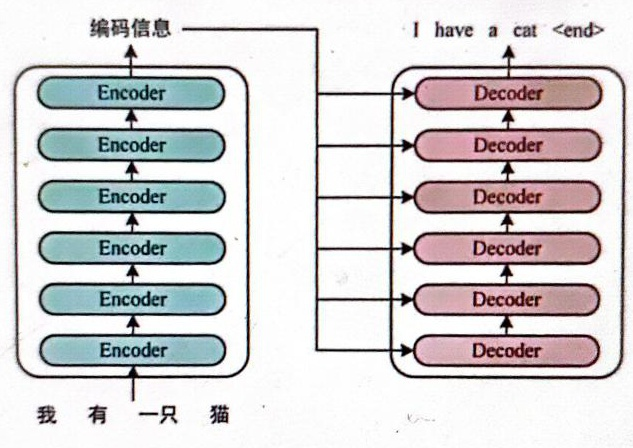
\includegraphics{images/image-0015.jpeg}
\caption{Transformer 的整体结构示意图}
\end{figure}

Transformer 的整体结构：左侧为 Encoder，右侧为 Decoder。

\begin{figure}[htbp]
\centering
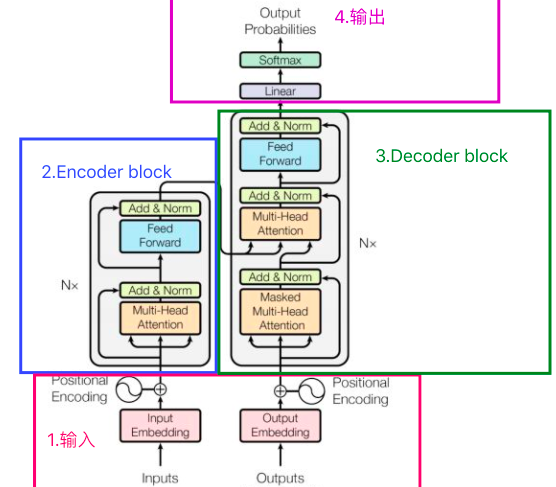
\includegraphics{images/image-0016.png}
\caption{Transformer 模块总览图}
\end{figure}

\hypertarget{ux4e00ux8f93ux5165}{%
\subsection{一、输入}\label{ux4e00ux8f93ux5165}}

\begin{enumerate}
\def\labelenumi{\arabic{enumi}.}
\item
  左下 inputs 表示输入序列，右下 Outputs (shifted right) 表示输出内容（其实是只提供该时间步以前生成的内容，训练预测能力）。
\item
  词嵌入 (Word Embedding)：每个词会被映射到一个固定长度的向量。例如，``猫''可能被表示为 \texttt{{[}0.1,\ -0.4,\ 0.8,\ ...{]}}。这些向量在训练开始时是随机的，模型会逐渐学习到让意思相近的词（如``猫''和``虎''）拥有更相似的向量。
\item
  位置编码 (Positional Encoding)：由于 Transformer 抛弃了 RNN 的顺序结构，后续的编码器本身无法感知词语的位置。没有位置信息，``我打你''和``你打我''在模型看来是一样的。为了解决这个问题，我们需要给每个词的向量中加入``位置信号''。后面会介绍位置编码。
\end{enumerate}

\hypertarget{ux4e8cencoder-block}{%
\subsection{二、Encoder Block}\label{ux4e8cencoder-block}}

\begin{enumerate}
\def\labelenumi{\arabic{enumi}.}
\item
  多头自注意力 (Multi-Head Attention)：编码器的核心，读取输入内容，通过多头自注意力机制，逐层得到富含上下文信息的中间表示。
\item
  Add：参照了残差神经网络，与输入直接相加。
\item
  Layer Normalization：对上一步的结果进行归一化处理。它能使模型训练过程更加稳定和快速，减少对参数初始化的敏感度。我们用 Layer Normalization (LN)，而不是 Batch Normalization (BN)，这二者的区别是：
\end{enumerate}

假设我们的输入数据形状为 {[}Batch\_Size, Seq\_Len, d\_model{]}，比如：{[}32, 10, 512{]}（32个句子，每句10个词，每个词512维）。

Batch Normalization (BN) 是``纵向切''，它固定特征维度，统计整个Batch的均值和方差。对于第i个特征维度（比如第0维），它会把这32个句子中、所有位置的词的第0维拿出来求平均。这在NLP中非常糟糕。因为不同句子的长度不同（通常靠Padding补齐），且不同位置的词语义差异极大，不同语段中各个特征维度的分布也往往有天然差异，强行让所有词语的第0维符合正态分布是不合理的，相当于``扭曲''了embedding空间，改变了向量之间的相似度，直接破坏embedding空间中存储的语义信息。

Layer Normalization (LN)是``横向切''，它固定样本（Token），统计该Token自身所有维度的均值和方差。对于第1个句子的第1个词（一个512维的向量），它计算这 512 个数值的均值和方差，然后进行伸缩，实质上抹平了向量模长的差异，让每个token的各个特征近似服从N(0,1)，这样点积就可以近似表示余弦相似度，即语义相似度。LN 将所有向量拉回到同一个``单位球壳''附近，让模型专注于学习方向（特征的组合方式，即语义），而不是数值的大小。

\begin{enumerate}
\def\labelenumi{\arabic{enumi}.}
\setcounter{enumi}{3}
\tightlist
\item
  Feed Forward：在每个注意力层之后，编码器和解码器都会有一个简单的前馈神经网络。这个网络对每个位置的向量独立地进行一次非线性变换。它由两个线性层和一个 ReLU 激活函数组成，可以看作是对注意力机制提取出的信息进行进一步的加工和提炼，增加模型的非线性能力。
\end{enumerate}

\hypertarget{ux4e09decoder-block}{%
\subsection{三、Decoder Block}\label{ux4e09decoder-block}}

\begin{enumerate}
\def\labelenumi{\arabic{enumi}.}
\tightlist
\item
  带掩码的多头自注意力 (Masked Multi-Head Self-Attention)
\end{enumerate}

（1）目的与工作方式：``回顾已写内容''。在生成下一个词时，解码器需要知道自己前面已经写了什么，以保证句子的连贯性。例如，已经写了 ``I am a''，下一个词很可能是 ``cat''，而不是重复生成 ``I''。它和编码器中的自注意力机制几乎完全一样，都是为了计算序列内部词与词之间的关系。

（2）为什么需要掩码？

在训练时，我们已经知道了完整的译文（例如 ``I am a cat''）。如果没有掩码，当模型在预测 ``am'' 这个词时，它会``偷看''到后面的 ``a'' 和 ``cat''，这显然是在作弊，模型学不到真正的预测能力。

（3）如何实现掩码？

掩码是一个``上三角矩阵''，它在计算注意力分数后、进行 Softmax 之前起作用。它会强制将所有未来位置 \((i,j)\)（\(i>j\)）的注意力分数，即 \(q_i\) 与 \(k_j\) 的点积设置为一个绝对值极大的负数（例如 \(-10^9\)）。

效果：绝对值极大的负数经过 Softmax 函数后，其对应的权重会无限接近于0。这样一来，模型在计算任意位置的输出时，其注意力权重只能分布在当前位置和之前的位置上，从而保证了模型无法``看到未来''。

\begin{enumerate}
\def\labelenumi{\arabic{enumi}.}
\setcounter{enumi}{1}
\tightlist
\item
  编码器-解码器注意力 (Encoder-Decoder Attention / Cross-Attention)
\end{enumerate}

（1）目的：这是连接编码器和解码器的核心桥梁。它让解码器在生成译文的每一步，都能去关注原文中最相关的部分。它用自己当前的理解(Q)去查询原文的完整信息 (K和V)，看看原文的哪一部分对生成下一个词最重要。

（2）工作方式：这也是一个多头注意力层，但它的 \(Q,K,V\) 来源不同：

查询向量 (Query, Q)：来自解码器前一个子层（即带掩码的自注意力层）的输出。这个 Q 向量代表了``写作部''当前的需求，可以理解为：``根据我已经写出的内容（比如 `I am'），我现在需要什么信息来决定下一个词？''

键向量 (Key, K) 和 值向量 (Value, V)：全部来自编码器栈的最终输出（即``理解部''的最终版精读笔记）。这两个向量代表了原文的完整信息，并且在解码的整个过程中是固定不变的。

（3）比喻：解码器（作者）拿着自己的草稿（Q 向量）去问编码器（原文摘要）：``我的草稿写到这了，请问你原文中哪部分内容跟我现在要写的最相关？'' 编码器通过 K, V 向量回答它，解码器据此获得生成下一个词的关键线索。例如，当解码器生成到与 ``猫'' 对应的位置时，这一层的注意力会高度集中在编码器输出中代表 ``猫'' 的那个向量上。

\begin{enumerate}
\def\labelenumi{\arabic{enumi}.}
\setcounter{enumi}{2}
\tightlist
\item
  前馈神经网络 (Position-wise Feed-Forward Network)
\end{enumerate}

（1）目的：``消化整合，深入思考''。

（2）工作方式：这个子层与编码器中的前馈网络完全相同。它接收来自编码器-解码器注意力层的输出向量，并对其进行一次非线性变换。

（3）比喻：在回顾了自己写的内容（Masked Self-Attention）并查阅了原文（Encoder-Decoder Attention）之后，解码器需要一个``独立思考''的过程，将这些信息进行整合、加工和提炼，最终形成一个准备用于预测下一个词的、信息高度浓缩的向量。这个``独立思考''的过程就是由前馈网络完成的。

\hypertarget{ux56dbux8f93ux51fa}{%
\subsection{四、输出}\label{ux56dbux8f93ux51fa}}

\begin{enumerate}
\def\labelenumi{\arabic{enumi}.}
\tightlist
\item
  取注意力层输出矩阵的什么内容？
\end{enumerate}

注意力层输出矩阵的形状为 \texttt{{[}seq\_len,d\_model{]}}，其中 \texttt{seq\_len} 是输入序列长度。

我们的目标是预测序列的 Next Token（如第4个词），我们只需要关注序列中最后一个 Token（第3个词）经过模型处理后的输出向量。因为在 Masked Self-Attention（带掩码的自注意力）机制下，最后一个 Token 的向量 \(h\) 已经聚合了整个序列的所有历史信息。

若希望得到原序列经过交互后富含上下文信息的序列：输出整个矩阵对应的Token序列。

\begin{enumerate}
\def\labelenumi{\arabic{enumi}.}
\setcounter{enumi}{1}
\tightlist
\item
  计算相似度
\end{enumerate}

得到输出向量后，我们会将其转化为输出 Token，具体操作为：和词表中所有 Token 计算点积相似度，这一步可以用矩阵乘法表示为 \(hW\)（\(W\) 是输出层的权重矩阵，每一行被视为词表中对应词的嵌入向量），经过 Softmax 后输出。

为什么可以用点积作为相似度呢？我们先从余弦相似度说起：

假设我们有两张不同的猫的图片，对应向量 \(x\) 和 \(y\)，我们希望它们的欧氏距离很小。在少数轮廓、皮毛之类的信号维度上，\(x_i\) 和 \(y_i\) 的值可能很相似，所以 \((x_i-y_i)^2\) 很小；但在草地、光照、拍摄角度等海量噪音维度上，\(x_i\) 和 \(y_i\) 会有微小的随机差异，每个 \((x_i-y_i)^2\) 可能不大，但它们的数量是压倒性的。

欧氏距离的 \(L_2\) 度量本质上是一个无差别的累加器：

\[
d^2(x,y)=\sum_{i\in\text{Signal}}(x_i-y_i)^2+\sum_{j\in\text{Noise}}(x_j-y_j)^2
\]

它将信号维度上的微小差异与海量噪音维度上的随机差异同等对待，并将它们的平方和累加起来。最终总距离的计算结果可能由噪音项的总和主导，因此并不适合作为高维语义向量的主要相似度度量。

余弦相似度衡量的是两个向量在方向上的接近程度，直接忽略它们的绝对长度：

\[
d_{\cos}(x,y)=\frac{x\cdot y}{\|x\|\|y\|}=\frac{\sum_{i=1}^{D}x_i y_i}{\sqrt{\sum_{i=1}^{D}x_i^2}\sqrt{\sum_{i=1}^{D}y_i^2}}
\]

方向是一种比长度更稳健的度量，承载了更纯净的各向异性信号：

\begin{itemize}
\tightlist
\item
  高维中随机的背景噪音几乎都是正交的，点积会非常接近 0。
\item
  而构成猫的信号维度在不同猫图片向量中表现出一致的方向性，点积可以增强这一点。
\end{itemize}

实际上，大模型中使用的多为点积相似度。原因：

（1）效率与简化计算\hspace{0pt}：点积运算 (A · B) 本身比余弦相似度计算（需要先计算点积，再除以两个向量的模长 \textbar\textbar A\textbar\textbar{} * \textbar\textbar B\textbar\textbar）更简单高效。在自回归生成中，模型需要为词表中的每一个词（通常是数万甚至数十万个）计算一个相似度分数，点积能显著减少计算量。

（2）与Softmax的天然配合：模型的学习过程已经内化了对向量``长度''的调整，各个向量长度几乎差不多。这时，点积计算得到的分数（通常称为 logits）会直接输入到 Softmax 函数中，以转换为下一个词的概率分布。所有词都除以模长或者都不除以模长对于经过 Softmax 函数后的概率分布没有影响，因此这一步可以被省略而不影响模型性能。

\begin{enumerate}
\def\labelenumi{\arabic{enumi}.}
\setcounter{enumi}{2}
\tightlist
\item
  自回归输出
\end{enumerate}

模型每次利用序列前文 \([x_1,\ldots,x_{i-1}]\) 作为输入，输出一个 token 即 \(x_i\)，再将 \([x_1,\ldots,x_i]\) 作为新的输入，以此类推。这个``输入 -\textgreater{} 解码器栈处理 -\textgreater{} 线性层 -\textgreater{} Softmax -\textgreater{} 选择词语''的循环会一直进行下去，直到选出的词是特殊的句子结束符 \texttt{\textless{}/s\textgreater{}} 为止。这个过程是串行的。

\hypertarget{ux53c2ux8003ux6587ux732e-68}{%
\subsection{参考文献}\label{ux53c2ux8003ux6587ux732e-68}}

\begin{itemize}
\tightlist
\item
  Vaswani, A., Shazeer, N., Parmar, N., et al.~(2017). \href{https://arxiv.org/abs/1706.03762}{Attention Is All You Need}. NeurIPS 2017.
\end{itemize}

\clearpage

\hypertarget{ux4f4dux7f6eux7f16ux7801}{%
\section{位置编码}\label{ux4f4dux7f6eux7f16ux7801}}

Transformer的标准处理流程中，并没有考虑token在序列的不同位置带来的差异。为了打上这个``补丁''，一般我们会运用基于正余弦的位置编码。

\hypertarget{ux4e00ux7ecfux5178transformerux7684ux6b63ux4f59ux5f26ux4f4dux7f6eux7f16ux7801}{%
\subsection{一、经典Transformer的正余弦位置编码}\label{ux4e00ux7ecfux5178transformerux7684ux6b63ux4f59ux5f26ux4f4dux7f6eux7f16ux7801}}

\hypertarget{ux4e00ux516cux5f0fux5f62ux5f0f}{%
\subsubsection{（一）公式形式}\label{ux4e00ux516cux5f0fux5f62ux5f0f}}

假设我们有一个输入序列，其长度为 \(L\)，模型的隐藏层维度（Embedding Dimension）为 \(d_{model}\)。对于序列中位置为 \(pos\) 的词（\(0 \le pos < L\)），以及该词向量中的第 \(i\) 个维度（\(0 \le i < d_{model}\)），其位置编码 \(PE\) 的计算公式如下：

\[
PE_{(pos,2i)}=\sin\left(\frac{pos}{10000^{2i/d_{model}}}\right)
\]

\[
PE_{(pos,2i+1)}=\cos\left(\frac{pos}{10000^{2i/d_{model}}}\right)
\]

对于每个位置，利用上面的函数可以生成一个位置向量，这个向量会和词的嵌入向量相加。``相加''意味着融合，模型在学习 token 的信息时，也同时学习到了位置信息。

\hypertarget{ux4e8cux539fux7406ux89e3ux91ca}{%
\subsubsection{（二）原理解释}\label{ux4e8cux539fux7406ux89e3ux91ca}}

\begin{enumerate}
\def\labelenumi{\arabic{enumi}.}
\tightlist
\item
  为什么使用正余弦？
\end{enumerate}

（1）有界性：位置编码向量的每一维都被控制在 \([-1,1]\)，不至于``喧宾夺主''压倒语义信息。

（2）对不同长度序列的适应性：

假设我们设定一个最大长度 \(L_{max}\)，位置 \(pos\) 的编码为：

\[
PE(pos)=\frac{pos}{L_{max}}
\]

如果 \(L_{max}\) 是针对当前句子长度动态设定的，就会出现致命缺陷：步长不一致。例如句子 A 长度为 5，第 1 个词是 0.0，第 2 个词是 0.2，相邻距离是 0.2；句子 B 长度为 100，第 1 个词是 0.0，第 2 个词是 0.01，相邻距离是 0.01。模型无法稳定学习``相邻''这个概念。

如果 \(L_{max}\) 是全局固定的极大值（比如 10000），当 \(L_{max}\) 很大时，相邻两个位置的差异 \(\Delta=\frac{1}{10000}\) 会非常微小。在深层神经网络中，这样微小的数值差异很容易被噪声淹没，导致模型很难区分位置 100 和位置 101。相比之下，正弦编码在高频分量上的数值变化非常剧烈，更容易区分相邻位置。

（3）位置可加性：由三角函数的性质

\[
\sin(\alpha+\beta)=\sin\alpha\cos\beta+\cos\alpha\sin\beta
\]

\[
\cos(\alpha+\beta)=\cos\alpha\cos\beta-\sin\alpha\sin\beta
\]

因此：

\[
\begin{pmatrix}
PE_{(pos+k,2i)} \\
PE_{(pos+k,2i+1)}
\end{pmatrix}
=
\begin{pmatrix}
\cos(\omega_i k) & \sin(\omega_i k) \\
-\sin(\omega_i k) & \cos(\omega_i k)
\end{pmatrix}
\begin{pmatrix}
PE_{(pos,2i)} \\
PE_{(pos,2i+1)}
\end{pmatrix}
\]

这是一个标准的旋转矩阵（Rotation Matrix）。结论是，\(PE_{(pos+k)}\) 确实可以由 \(PE_{(pos)}\) 乘以一个与 \(pos\) 无关、仅与 \(k\) 有关的线性变换矩阵得到。这使得 Self-Attention 机制能够很容易地学会关注``距离当前词 \(k\) 个单位''的词，即具备了捕捉相对位置的能力。

\begin{enumerate}
\def\labelenumi{\arabic{enumi}.}
\setcounter{enumi}{1}
\tightlist
\item
  为什么位置编码是一个 \(d_{model}\) 维的向量，对于每一个特征维度 \(i\) 都不一样？
\end{enumerate}

首先明确：虽然语义编码和位置编码维数相同，但二者的第i维之间没有物理意义上的一一对应。

为什么位置编码需要 \(d_{model}\) 维呢？这是因为在一个长序列中，如果只用一维表征信息，会出现严重的问题。比如序列有一百万个 token，那么在一圈弧度为 \(2\pi\) 的情况下，第 5 个和第 15 个 token 之间的角度就是 \(2 \times 10^{-5}\pi\)，在三角函数运算后差距几乎为零，淹没在随机噪声中。

同时，让所有维度的位置编码都用同一个值还会带来两个问题。首先是会让语义向量沿 \((1,1,\ldots)\) 的统一方向移动，而这个方向可能本来要表征其他语义。其次是 Layer Normalization 过程中会对每个向量进行归一化：

\[
\mathrm{LN}(x)=\frac{x-\mu}{\sigma}\cdot\gamma+\beta
\]

这会直接把位置编码``清洗''掉。

因此，我们需要增加维度。就像一个一位布尔值只能表示 0 或 1，但是八位编码却能表示 256 个数值。利用三角函数的旋转特性，我们想到可以用一个有 \(d_{model}\) 根指针的``时钟''，将编码的高位数存在低频率旋转的``时针''中，低位数存在高频率旋转的``秒针''中：

我们可以将分母 \(10000^{2i/d_{model}}\) 理解为波长，或者将其倒数理解为频率。令频率 \(\omega_i=\frac{1}{10000^{2i/d_{model}}}\)，则公式可简化为：

\[
PE_{(pos,2i)}=\sin(\omega_i\cdot pos)
\]

\[
PE_{(pos,2i+1)}=\cos(\omega_i\cdot pos)
\]

\begin{itemize}
\tightlist
\item
  低维度（\(i\) 较小）：\(\omega_i\) 较大，波长短，变化频率高。
\item
  高维度（\(i\) 较大）：\(\omega_i\) 极小，波长极长，变化频率低。
\end{itemize}

在 Transformer 的公式中，分母 \(10000^{2i/d}\) 就是波长 \(\lambda_i\)。例如：

\begin{itemize}
\tightlist
\item
  当 \(i=0\)（第 0 维）时，分母是 \(10000^0=1\)。这是一个超短波，\(pos\) 每增加 \(2\pi\)（约 6 个词），正弦波就跑完一整圈。作用：它像一把``游标卡尺''，负责精确区分相邻的、微小的位置变化（比如 \(pos=5\) 和 \(pos=6\)）。
\item
  当 \(i=256\)（第 512 维）时，分母是 \(10000^1=10000\)。这是一个超长波，\(pos\) 需要增加 \(10000\cdot2\pi\)（约 6 万个词），正弦波才跑完一圈。作用：它像一把``公里计数器''，在短句子里几乎是一条直线，负责提供宏观的、全局的定位。
\end{itemize}

\begin{enumerate}
\def\labelenumi{\arabic{enumi}.}
\setcounter{enumi}{2}
\tightlist
\item
  为什么波长不能线性增长，而要用 \(10000^{2i/d}\) 这种指数形式？
\end{enumerate}

想象你要用几个数字转盘来表示从 0 到 10000 的数字：

\begin{itemize}
\tightlist
\item
  线性方案（极低效）：如果你有 3 个转盘，分别代表 1s、2s、3s，你能表示的范围非常窄，或者你需要成千上万个转盘才能数到 10000。
\item
  指数方案（十进制/位值制）：你有 3 个转盘，分别代表：

  \begin{itemize}
  \tightlist
  \item
    转盘 A：\(10^0=1\)（个位）
  \item
    转盘 B：\(10^1=10\)（十位）
  \item
    转盘 C：\(10^2=100\)（百位）
  \end{itemize}
\end{itemize}

注意到了吗？1、10、100 就是指数级增长的。仅仅用 3 个维度（个、十、百），我们就能覆盖很大的范围，而且每个数字的表示都是唯一的。

Transformer 的 512 个维度也是这个道理：我们不希望第 10 维和第 11 维的波长差不多（比如 50 和 51），那样太浪费了。我们希望它们成倍增长。通过指数级的波长分配，512 个维度均匀地覆盖了从 \(2\pi\) 到 \(10000\cdot2\pi\) 的巨大范围，这让模型在对数尺度（Log Scale）上拥有了均匀的分辨率。

\hypertarget{ux4e8cux65cbux8f6cux4f4dux7f6eux7f16ux7801rope}{%
\subsection{二、旋转位置编码（RoPE）}\label{ux4e8cux65cbux8f6cux4f4dux7f6eux7f16ux7801rope}}

RoPE 是目前各大主流语言模型（如 LLaMA、Qwen）标配的位置编码方式。它不像上面那样直接``加上''一个位置向量，而是通过在复平面上的``旋转''来注入位置信息，从而自带相对位置信息的感知能力。

对于一个位置为 \(m\) 的输入向量 \(x=[x_1,x_2,\ldots,x_d]^T\)，RoPE 将相邻的两个维度视为一组二维坐标，并根据位置 \(m\) 乘以一个旋转矩阵。其完整的块对角旋转矩阵 \(R_{\Theta,m}^{d}\) 表达式如下：

\[
\begin{pmatrix}
\cos(m\theta_1) & -\sin(m\theta_1) & 0 & 0 & \cdots & 0 & 0 \\
\sin(m\theta_1) & \cos(m\theta_1) & 0 & 0 & \cdots & 0 & 0 \\
0 & 0 & \cos(m\theta_2) & -\sin(m\theta_2) & \cdots & 0 & 0 \\
0 & 0 & \sin(m\theta_2) & \cos(m\theta_2) & \cdots & 0 & 0 \\
\vdots & \vdots & \vdots & \vdots & \ddots & \vdots & \vdots \\
0 & 0 & 0 & 0 & \cdots & \cos(m\theta_{d/2}) & -\sin(m\theta_{d/2}) \\
0 & 0 & 0 & 0 & \cdots & \sin(m\theta_{d/2}) & \cos(m\theta_{d/2})
\end{pmatrix}
\]

其中，旋转角 \(\theta_i=10000^{-2(i-1)/d}\)。最终注入了位置信息的特征向量即为 \(x'_m=R_{\Theta,m}^{d}x\)。

对于非一维的序列（如视频），既然视频是 3D 数据（时间、高度、宽度），V-JEPA 2 采用的是 1D-RoPE 的 3D 扩展版本。具体的做法是：将总的特征维度 \(d\) 平分为三个大致相等的部分：\(d_t\)（时间轴）、\(d_h\)（高度轴）和 \(d_w\)（宽度轴）。对于视频中的某一个 Patch，假设它在时间帧上的坐标为 \(t\)，空间坐标为 \((h,w)\)，则分别对这三个特征分段应用对应维度的 1D 旋转。

\hypertarget{ux53c2ux8003ux6587ux732e-69}{%
\subsection{参考文献}\label{ux53c2ux8003ux6587ux732e-69}}

\begin{itemize}
\tightlist
\item
  Vaswani, A., Shazeer, N., Parmar, N., et al.~(2017). \href{https://arxiv.org/abs/1706.03762}{Attention Is All You Need}. NeurIPS 2017.
\item
  Su, J., Lu, Y., Pan, S., Wen, B., \& Liu, Y. (2021). \href{https://arxiv.org/abs/2104.09864}{RoFormer: Enhanced Transformer with Rotary Position Embedding}. arXiv:2104.09864.
\end{itemize}

\clearpage

\hypertarget{bert}{%
\section{BERT}\label{bert}}

\hypertarget{ux4e00ux6838ux5fc3ux601dux60f3ux57faux4e8etransformerux7684ux53ccux5411ux4e0aux4e0bux6587ux7f16ux7801ux5668}{%
\subsection{一、核心思想：基于Transformer的双向上下文编码器}\label{ux4e00ux6838ux5fc3ux601dux60f3ux57faux4e8etransformerux7684ux53ccux5411ux4e0aux4e0bux6587ux7f16ux7801ux5668}}

BERT的核心思想在于：要真正理解一个词的含义，必须同时考虑它左右两侧的所有上下文。它通过一种称为~``双向编码器''~的架构来实现这一点。BERT的模型架构基础是Google在2017年提出的Transformer模型，但BERT只使用了Transformer的编码器部分，BERT-base模型由12层Transformer编码器堆叠而成，BERT-large则有24层。

注意力机制是Transformer的核心，也是BERT实现双向理解的关键。它允许序列中的任何一个词直接与序列中的所有其他词进行交互，计算它们之间的关联权重。通过这种方式，模型在处理每个词时，都``注意''到了整个句子的信息。此外，在输入词的嵌入向量中加入了位置编码，告诉模型每个词在序列中的具体位置。

\hypertarget{ux4e8cux5173ux952eux6280ux672fux4e24ux5927ux9884ux8badux7ec3ux4efbux52a1}{%
\subsection{二、关键技术：两大预训练任务}\label{ux4e8cux5173ux952eux6280ux672fux4e24ux5927ux9884ux8badux7ec3ux4efbux52a1}}

BERT的强大能力还来自其开创性的预训练方法。它在海量无标注文本上通过两个巧妙的``完形填空''任务进行训练，从而学习到通用的语言表示。一般以下两个任务同时进行。

\begin{enumerate}
\def\labelenumi{\arabic{enumi}.}
\tightlist
\item
  掩码语言模型（Masked Language Model, MLM）
\end{enumerate}

操作：在输入序列中，随机地遮盖（Mask）掉15\%的词语（用~{[}MASK{]}~标记替换）。

任务：模型的任务是预测这些被遮盖的原始词语是什么。

目的：这一步是实现BERT``双向性''的关键。这种方法强制模型必须根据上下文中的所有词（包括被遮盖词左右两边的词）来重建被遮盖的词，从而学会了深层的双向语言表征。

技巧：在这15\%的被选中的词中，并不是全部替换为~{[}MASK{]}。80\%的时间替换为~{[}MASK{]}；10\%的时间替换为一个随机的词，引入噪声，防止模型过于``自信''，增强模型的鲁棒性；10\%的时间保持原词不变，因为在微调阶段，输入的都是真实的、未被修改的词语。这10\%的情况让模型在预训练时也能接触到完整的、未被破坏的原始句子，使得预训练和微调的数据环境更加接近，也让模型知道``苹果''在这个上下文中是合理的，并且需要为其生成一个好的上下文向量表示。

改进：Span-Mask

BERT 的预训练目标（Masked Language Model, MLM）是随机选择序列中 15\% 的单个 token（令牌，可以理解为单词或子词），然后用 {[}MASK{]} 标签替换它们。如The quick brown {[}MASK{]} jumps {[}MASK{]} the lazy dog.模型需要独立地预测每个 {[}MASK{]} 位置上原来的 token (例如 fox 和 over)，可以利用 jumps 和 the 来预测 over，而不需要真正理解 jumps over 这个短语的含义。

Span-Mask的改进是，这种方法不再掩盖单个、分散的 token，而是选择一个连续的文本``跨度''（Span），并将这个连续片段中的所有 token 都替换掉。如假设我们要掩盖 quick brown fox 这个 span，输入The {[}MASK{]} {[}MASK{]} {[}MASK{]} jumps over the lazy dog.模型现在必须一次性地重建整个被掩盖的 quick brown fox 片段，模型不仅要预测被掩盖的 token 是什么，还必须知道内部结构（预测出 quick、brown 和 fox 之间的顺序和关系）以及跨度长度（模型需要学习到它应该生成三个 token 来填补这个空白，而不是一个或两个）。

总之，这可以强迫模型学习更丰富的上下文信息、序列的内部结构以及被掩盖片段的长度。这被认为是一个比标准 BERT 的 MLM 更难、也更有效的预训练任务。比如，对于蛋白质序列来说，这意味着模型不是在预测单个被掩盖的氨基酸，而是在预测一个连续的氨基酸片段，这可能迫使模型更好地学习蛋白质的局部结构或功能基序 (motif)。

\begin{enumerate}
\def\labelenumi{\arabic{enumi}.}
\setcounter{enumi}{1}
\tightlist
\item
  下一句预测（Next Sentence Prediction, NSP）
\end{enumerate}

为了让模型理解句子之间的关系（这对于问答、自然语言推理等任务至关重要），BERT增加了这个任务。

操作：在训练时，给模型输入两个句子A和B，其中50\%的情况下B是A的真实下一句（标签为~IsNext），另外50\%的情况下B是从语料库中随机抽取的（标签为~NotNext）。

任务：模型需要判断句子B是否是句子A的下一句。

目的：使模型能够捕捉两个文本片段之间的逻辑和语义关系。

\hypertarget{ux4e09ux5faeux8c03ux65b9ux5f0f}{%
\subsection{三、微调方式}\label{ux4e09ux5faeux8c03ux65b9ux5f0f}}

由于BERT本质是一个编码器，所以将其运用于特定的下游任务（如情感分类、问答、命名实体识别）时，只需要在BERT后面加一个简单的输出层（如一个全连接层），使用有标签的任务数据对这个模型进行端到端的精细调整即可。由于模型已经在通用语言上有了很好的基础，只需要少量数据微调就能在特定任务上取得极佳的效果。

\hypertarget{ux56dbux8f93ux5165ux8868ux793a}{%
\subsection{四、输入表示}\label{ux56dbux8f93ux5165ux8868ux793a}}

BERT的输入能够统一表示一个句子或一个句子对（如\textless 问题，答案\textgreater）。输入序列由三种嵌入向量求和而成：

词嵌入：将每个词转换成的向量。

段落嵌入：一个学习到的向量，用于区分句子A和句子B。例如，句子A的所有词都用~EA，句子B的所有词都用~EB。

位置嵌入：表示每个词在序列中位置信息的向量。

此外，每个序列的开头都有一个特殊的~{[}CLS{]}~标记，该标记的最终输出向量常用于分类任务（如情感分析）。句子之间用~{[}SEP{]}~标记分隔。

\hypertarget{ux4e94ux8f93ux51faux8868ux793aux591aux5c42ux7ea7ux7684ux8bedux4e49ux5411ux91cf}{%
\subsection{五、输出表示：多层级的语义向量}\label{ux4e94ux8f93ux51faux8868ux793aux591aux5c42ux7ea7ux7684ux8bedux4e49ux5411ux91cf}}

经过L层（BERT-base为12层）Transformer编码器的复杂计算与交互后，BERT最终会输出一个包含了丰富语义信息的张量。这个输出根据下游任务的需求，主要分为两种形式：

\begin{enumerate}
\def\labelenumi{\arabic{enumi}.}
\tightlist
\item
  序列输出
\end{enumerate}

这是BERT最基础、最原本的输出形式。假设输入序列的长度为N（包含{[}CLS{]}和{[}SEP{]}标记），隐藏层的维度为d\_model（BERT-base为768）。那么，序列输出可以表示为一个N*d\_model维矩阵：H = {[}h\_CLS, h\_1, h\_2, \ldots, h\_n, h\_SEP{]}，每一个h\_i都是一个维度为768的上下文相关的动态词向量。由于注意力机制的存在，向量h\_i虽然对应位置i的词，但它实际上融合了整个句子中所有其他词的信息。例如，在``苹果掉在地上''和``苹果手机发布会''中，尽管输入都是``苹果''，但输出的对应向量h\_apple是完全不同的。

适用任务：适用于词/Token级别的任务，如命名实体识别（对每个词进行分类）、问答系统（寻找答案在文章中的``起始位置''和``结束位置''）等。

\begin{enumerate}
\def\labelenumi{\arabic{enumi}.}
\setcounter{enumi}{1}
\tightlist
\item
  池化输出
\end{enumerate}

BERT使用序列第一个位置的特殊标记{[}CLS{]}的最终向量h\_CLS来代表整个句子的语义，它是一个高度压缩的、融合了全句核心意图的向量，是整个输入序列的``身份证''。一般会让h\_CLS再经过一个``池化层''，包括一个全连接层和tanh 激活函数，以让输出更适合作为分类任务的特征。

适用任务：适用于句子级别（Sentence-level）的任务，如：情感分析（判断句子是褒义还是贬义）、句子关系判断、下一句预测等。

\hypertarget{ux53c2ux8003ux6587ux732e-70}{%
\subsection{参考文献}\label{ux53c2ux8003ux6587ux732e-70}}

\begin{itemize}
\tightlist
\item
  Devlin, J., Chang, M.-W., Lee, K., \& Toutanova, K. (2019). \href{https://arxiv.org/abs/1810.04805}{BERT: Pre-training of Deep Bidirectional Transformers for Language Understanding}. NAACL 2019.
\item
  Joshi, M., Chen, D., Liu, Y., Weld, D. S., Zettlemoyer, L., \& Levy, O. (2020). \href{https://arxiv.org/abs/1907.10529}{SpanBERT: Improving Pre-training by Representing and Predicting Spans}. TACL.
\end{itemize}

\clearpage


% 大语言模型的基本原理
\hypertarget{ux5927ux8bedux8a00ux6a21ux578bux7684ux57faux672cux539fux7406}{%
\chapter{大语言模型的基本原理}\label{ux5927ux8bedux8a00ux6a21ux578bux7684ux57faux672cux539fux7406}}

\hypertarget{gptux4e0eux9884ux8badux7ec3}{%
\section{GPT与预训练}\label{gptux4e0eux9884ux8badux7ec3}}

\hypertarget{ux4e00ux6838ux5fc3ux601dux60f3-5}{%
\subsection{一、核心思想}\label{ux4e00ux6838ux5fc3ux601dux60f3-5}}

GPT（Generative Pre-trained Transformer）的核心思想是``预测 next token''，这是一个单向、自回归的生成过程。比如，第一次根据已有提示词，预测第一个 token（记为 \(x_1\)）；第二次根据提示词和 \(x_1\)，预测第二个 token \(x_2\)；第三次根据提示词和 \(x_1\)、\(x_2\)，预测第三个 token \(x_3\)\ldots\ldots 这样做的背后逻辑在于：一个真正强大的语言模型，仅仅通过``预测下一个词''这个任务，就能学到关于语言、知识、推理和思维的几乎所有规律。当模型的规模（参数、数据、算力）足够大时，这个看似简单的任务会迫使模型构建一个极其复杂和精确的对世界的模型，以便做出更好的预测。这个训练过程称为``预训练''（Pre-training），以和后续的微调（后训练）相区分。

事实上，这样的模型训练过程相当于将丰富的对世界的认识``压缩''在了模型参数中。有观点认为``压缩即智能''，因为为了在生成过程中获得高置信度的还原，模型必须从海量知识中提炼出内在规律，在训练时尽可能接近``无损压缩''。而这个提炼的过程也会让模型发现人类可能无法发现的一些不同领域知识间的内在关联，这也是创新的源泉之一（所以我们不能武断地认为 AI 不能创新）。当然，强化微调（后面会提到）也是 AI 能产生新策略的一个重要原因。

另外特别说明，这里的 GPT 指的是``生成式预训练 Transformer''这样一个通用架构，而并非特指 OpenAI 的 ChatGPT 系列模型（当然 ChatGPT 作为首个生成式 AI 产品，应该就是因这样的架构而命名的）。

\hypertarget{ux4e8cux6a21ux578bux67b6ux6784-1}{%
\subsection{二、模型架构}\label{ux4e8cux6a21ux578bux67b6ux6784-1}}

GPT 和 BERT 一样基于 Transformer，但和 BERT 不同的是，GPT 选用了 Transformer 架构的解码器部分，在三个注意力块中也只选用了其中的带掩码的多头自注意力（Masked Multi-Head Self-Attention）。

在这个注意力块中，查询、键、值均来自同一序列的已生成部分，每个词只能关注到它左边的词（即过去的词），而不能关注到它右边（即未来）的词，这决定了 GPT 的``单向性''。这是通过一个注意力掩码来实现的，它将未来位置的信息全部遮盖掉，确保模型在生成下一个词时，不会``偷看''到未来的答案，这与模型在推理时（生成模式）的行为保持一致。

GPT 模型由多层 Transformer 解码器块堆叠而成。例如，GPT-3 有 96 层。每个解码器块内部都包含一个全连接前馈网络，用于对每个位置的表示进行非线性变换。

为什么选择解码器？解码器的自回归特性天然契合``下一个词预测''的预训练任务。模型在训练时和推理时的行为是完全一致的，都是根据已知文本来预测未知文本，这避免了 BERT 存在的预训练-微调不一致问题。

\hypertarget{ux4e09ux4e3aux4ec0ux4e48ux4e0dux9700ux8981ux7f16ux7801ux5668ux4e3aux4ec0ux4e48ux6548ux679cux6bd4ux57faux4e8eux7f16ux7801ux5668ux7684-bert-ux66f4ux597d}{%
\subsection{三、为什么不需要编码器\&为什么效果比基于编码器的 BERT 更好？}\label{ux4e09ux4e3aux4ec0ux4e48ux4e0dux9700ux8981ux7f16ux7801ux5668ux4e3aux4ec0ux4e48ux6548ux679cux6bd4ux57faux4e8eux7f16ux7801ux5668ux7684-bert-ux66f4ux597d}}

\hypertarget{ux751fux6210ux80fdux529bux662fux66f4ux6839ux672cux66f4ux901aux7528ux7684ux80fdux529b}{%
\subsubsection{1. 生成能力是更根本、更通用的能力}\label{ux751fux6210ux80fdux529bux662fux66f4ux6839ux672cux66f4ux901aux7528ux7684ux80fdux529b}}

理解是生成的子集：要想高质量地生成一段文本，模型必须深刻地理解语言、知识、逻辑和上下文。一个能和你流畅对话的模型，其理解能力必然不差。反之，一个只擅长理解的模型（如 BERT），却无法进行流畅的生成。而通过``生成''范式，GPT 可以被引导去完成几乎任何 NLP 任务，这被称为``提示工程''。这种统一性使得一个模型可以应对千变万化的任务，而 BERT 通常需要为每个任务设计特定的模型结构和微调过程。

\hypertarget{scaling-law}{%
\subsubsection{2. Scaling Law}\label{scaling-law}}

大量实验发现，纯解码器的 Transformer 架构在当模型参数规模、数据量和计算力扩大到一定程度时，模型会涌现出令人惊讶的新能力（如推理、代码生成、复杂指令跟随等）。

当参数达到千亿级别（如 GPT-3）时，纯解码器架构涌现出了强大的上下文学习能力。这意味着，仅仅通过一个提示（Prompt），模型就能理解并执行各种复杂任务，而无需一个专门的编码器来为其解析指令。

这最终证明：一个足够庞大的自回归模型，其解码器本身就已经具备了我们期望编码器拥有的``深度理解''能力。它通过在生成过程中``反复咀嚼''前文，同样可以完成深度的语义理解。

\hypertarget{ux9884ux8badux7ec3ux4e0eux4f7fux7528ux4efbux52a1ux7684ux4e00ux81f4ux6027}{%
\subsubsection{3. 预训练与使用任务的一致性}\label{ux9884ux8badux7ec3ux4e0eux4f7fux7528ux4efbux52a1ux7684ux4e00ux81f4ux6027}}

GPT 的训练任务是下一个词预测（自回归），GPT 的推理/使用方式也是生成下一个词，并将其作为新的输入，继续生成下一个词（自回归）。模型在训练时和部署时的行为是完全一致的。它永远不会在训练时看到整个句子（因为未来词被掩码遮住了），在推理时也不需要看到未来词。这种一致性使得模型能够将其在训练中学到的所有能力，毫无损耗地应用到实际生成中。

反之，如果 GPT 在预训练时使用了编码器（双向注意力）来理解输入，那么在推理生成时就会遇到一个悖论：在生成第 \(N\) 个词时，编码器需要看到完整的输入序列才能进行编码，但完整的输入序列包含了尚未生成的未来词。因此，为了保持极致的任务一致性，抛弃编码器是必然的选择。

而训练过程与生成任务的不一致性也被认为是制约 BERT 性能（尤其是生成方面性能）的瓶颈之一。

\hypertarget{ux7f16ux7801ux5668ux7684ux5197ux4f59ux6027}{%
\subsubsection{4. 编码器的冗余性}\label{ux7f16ux7801ux5668ux7684ux5197ux4f59ux6027}}

编码器-解码器架构是为序列到序列任务设计的，比如机器翻译、文本摘要。这些任务的特点是输入和输出可以是不同长度、不同模态的，编码器要理解、编码整个输入序列（双向），再由解码器负责根据编码器的输出，自回归地生成输出序列，而 GPT 的任务更像是``文本续写''，而不是``文本转换''。

从参数和计算效率上，只训练一个解码器栈，相比训练编码器和解码器两个栈，在参数量相同的情况下，每个组件可以更``深''或更``宽''，模型能力可能更强。训练和推理过程也更简单，避免了编码器和解码器之间的复杂交互。

一个比喻：编码器-解码器（如 T5）像是一个翻译团队。编码器是分析源语言的研究员（全面理解原文），解码器是根据研究员报告撰写目标语言的作家（生成译文）；纯解码器（如 GPT）像是一个独自创作的作家。他一边阅读自己已经写下的前文（这本身就是``理解''过程），一边续写后面的内容。他不需要一个独立的研究员来告诉他前文是什么意思，因为他自己就是作者。

\hypertarget{ux6587ux672cux81eaux8eabux7684ux5e8fux5217ux6027}{%
\subsubsection{5. 文本自身的序列性}\label{ux6587ux672cux81eaux8eabux7684ux5e8fux5217ux6027}}

BERT 为代表的编码器架构在模型规模极大时，可能不如自回归的解码器有效，因为它破坏了文本的天然序列性。

\hypertarget{ux56dbux591aux6a21ux6001}{%
\subsection{四、多模态}\label{ux56dbux591aux6a21ux6001}}

多模态技术，就是让 AI 从单纯的``文字处理者''进化为具备``眼耳口脑''的全能感知体。它打破了文本、图像、音频和视频之间的壁垒，能够像人类一样同时通过看图、听声音和读文字来理解世界；例如，你不仅可以用文字提问，还能直接上传一段视频或一张图表让 AI 分析其中的逻辑。

目前主流的实现方法是通过一些方式，将各个模态的信息``对齐''到统一的高维语义空间中进行处理，从而在预训练中融合多个模态的数据。无论输入的是文本、图像还是音频，输入信息经过不同方式处理后，最终都会统一到同一个高维语义空间中。比如，``猫''这个词语和一张猫的图片在这个语义空间中距离较近，和一张西瓜的图片在空间中距离较远。具体实现方式可见多模态部分介绍。

\hypertarget{ux53c2ux8003ux6587ux732e-71}{%
\subsection{参考文献}\label{ux53c2ux8003ux6587ux732e-71}}

\begin{itemize}
\tightlist
\item
  Vaswani, A., Shazeer, N., Parmar, N., et al.~(2017). \href{https://arxiv.org/abs/1706.03762}{Attention Is All You Need}. NeurIPS 2017.
\item
  Radford, A., Narasimhan, K., Salimans, T., \& Sutskever, I. (2018). \href{https://cdn.openai.com/research-covers/language-unsupervised/language_understanding_paper.pdf}{Improving Language Understanding by Generative Pre-Training}. OpenAI.
\item
  Radford, A., Wu, J., Child, R., et al.~(2019). \href{https://cdn.openai.com/better-language-models/language_models_are_unsupervised_multitask_learners.pdf}{Language Models are Unsupervised Multitask Learners}. OpenAI.
\item
  Brown, T. B., Mann, B., Ryder, N., et al.~(2020). \href{https://arxiv.org/abs/2005.14165}{Language Models are Few-Shot Learners}. NeurIPS 2020.
\end{itemize}

\clearpage

\hypertarget{ux8bcdux5d4cux5165embedding}{%
\section{词嵌入（Embedding）}\label{ux8bcdux5d4cux5165embedding}}

\hypertarget{ux4e00ux8bcdux5d4cux5165embeddingux7684ux6574ux4f53ux6d41ux7a0b}{%
\subsection{一、词嵌入（Embedding）的整体流程}\label{ux4e00ux8bcdux5d4cux5165embeddingux7684ux6574ux4f53ux6d41ux7a0b}}

Tokenizer（分词器）把句子切分成词（Token），然后去词表里查出每个词对应的整数ID。词嵌入层（Embedding Layer）接收Tokenizer输出的整数ID，并将其转化为包含语义的浮点数向量，供后续的Attention层进行处理。

\hypertarget{ux4e8ctokenizerux5206ux8bcdux5668}{%
\subsection{二、Tokenizer（分词器）}\label{ux4e8ctokenizerux5206ux8bcdux5668}}

输入一个原始文本字符串，如``The cat sat''。Tokenizer先将字符串分解为``词元''(Token)，再根据一个在训练前就构建好的、从``词''到``ID''的映射字典，每个 Token 转换为其对应的整数 ID。如{[}``the'', ``cat'', ``sat''{]}转化为{[}2, 3, 4{]}，不是训练的对象。

\hypertarget{ux4e09embedding-layerux8bcdux5d4cux5165ux5c42}{%
\subsection{三、Embedding Layer（词嵌入层）}\label{ux4e09embedding-layerux8bcdux5d4cux5165ux5c42}}

它是神经网络内部的第一个层，输入是Tokenizer输出的整数ID序列，如{[}2, 3, 4{]}，输出这些ID对应的向量拼接成的矩阵。在数学上，这个过程可以用矩阵线性计算（无激活函数）表示。它的参数是每个Token的embedding向量表示，例如词汇表有 50,000 个词，每个词是一个300维向量，那这一层的参数量就是15,000,000。训练时根据输入和输出更新参数，通过参数的正确收敛（每个词嵌入向量能有效表达语义），实现对输入文段的正确输出表示。测试时，根据前向计算，得出每个Token的ID对应的嵌入向量。例如算出代表 ``the'' 的 300 维向量为{[}0.12, -0.45, \ldots, 0.88{]} ，代表 ``cat'' 的{[}0.67, 0.01, \ldots, -0.23{]}，代表 ``sat'' 的{[}-0.11, 0.98, \ldots, 0.51{]} ，输出{[}{[}0.12, \ldots{]}, {[}0.67, \ldots{]}, {[}-0.11, \ldots{]}{]}。

例如句子 \texttt{Don\textquotesingle{}t\ you\ love\ {[}emoji{]}\ Transformers?\ We\ sure\ do.} 在不同分词器下会得到不同的 Token 序列和 ID 序列：

\begin{itemize}
\tightlist
\item
  根据空格分词：\texttt{{[}"Don\textquotesingle{}t",\ "you",\ "love",\ "{[}emoji{]}",\ "Transformers?",\ "We",\ "sure",\ "do."{]}}，对应的 ID 序列为 \texttt{{[}1347,\ 249,\ 890,\ 1310,\ 8219,\ 568,\ 909,\ 791{]}}。
\item
  根据 spaCy 分词器分词：\texttt{{[}"Do",\ "n\textquotesingle{}t",\ "you",\ "love",\ "{[}emoji{]}",\ "Transformers",\ "?",\ "We",\ "sure",\ "do",\ "."{]}}，对应的 ID 序列为 \texttt{{[}91,\ 8123,\ 21313,\ 3123,\ 41251,\ 151,\ 9859,\ 115,\ 1515,\ 3134,\ 4114{]}}。
\end{itemize}

\hypertarget{ux53c2ux8003ux6587ux732e-72}{%
\subsection{参考文献}\label{ux53c2ux8003ux6587ux732e-72}}

\begin{itemize}
\tightlist
\item
  Vaswani, A., Shazeer, N., Parmar, N., et al.~(2017). \href{https://arxiv.org/abs/1706.03762}{Attention Is All You Need}. NeurIPS 2017.
\item
  Radford, A., Narasimhan, K., Salimans, T., \& Sutskever, I. (2018). \href{https://cdn.openai.com/research-covers/language-unsupervised/language_understanding_paper.pdf}{Improving Language Understanding by Generative Pre-Training}. OpenAI.
\end{itemize}

\clearpage

\hypertarget{ux751fux6210ux8fc7ux7a0bux7684ux5e72ux9884}{%
\section{生成过程的干预}\label{ux751fux6210ux8fc7ux7a0bux7684ux5e72ux9884}}

\hypertarget{ux4e00ux6e29ux5ea6temperature}{%
\subsection{一、温度（Temperature）}\label{ux4e00ux6e29ux5ea6temperature}}

\begin{itemize}
\tightlist
\item
  \textbf{高温值（如 1.0）}：增加生成结果的多样性，但可能导致结果不稳定。
\item
  \textbf{低温值（如 0.1）}：生成结果更稳定，但可能缺乏创造性。
\end{itemize}

温度参数控制生成结果的随机性。具体来说，温度参数 \(T\) 影响概率分布的``尖锐度''。温度越高，概率分布越平滑，生成结果的多样性越高；温度越低，概率分布越尖锐，生成结果越稳定。

\[
P(x_{T+1} \mid x_1, x_2, \ldots, x_T) =
\frac{\exp\left(\frac{f(x_1,x_2,\ldots,x_T)}{T}\right)}
{\sum_i \exp\left(\frac{f_i(x_1,x_2,\ldots,x_T)}{T}\right)}
\]

其中，\(f(x_1,x_2,\ldots,x_T)\) 是模型的内部函数，通常是一个复杂的神经网络，如 Transformer 架构。\(T\) 是温度参数，控制概率分布的平滑程度。

\hypertarget{ux4e8cux91c7ux6837ux641cux7d22ux8bcdux5143ux7b56ux7565}{%
\subsection{二、采样（搜索词元）策略}\label{ux4e8cux91c7ux6837ux641cux7d22ux8bcdux5143ux7b56ux7565}}

\hypertarget{ux8d2aux5fc3ux641cux7d22}{%
\subsubsection{贪心搜索}\label{ux8d2aux5fc3ux641cux7d22}}

始终选择概率最高的下一个词，生成结果稳定但可能单调。

\[
x_{T+1} = \arg\max P(x_{T+1} \mid x_1, x_2, \ldots, x_T)
\]

贪心搜索示例：图片展示了一个树状图，从 ``The'' 开始，每一步都选择概率最高的分支，例如 The -\textgreater{} nice (0.5) -\textgreater{} woman (0.4) \ldots{}

\begin{figure}[htbp]
\centering
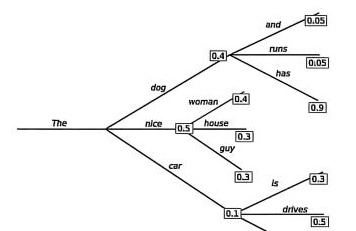
\includegraphics{images/image-0017.jpeg}
\caption{贪心搜索树状示例}
\end{figure}

问题：每步取最高≠乘积最高！

\hypertarget{ux6ce2ux675fux641cux7d22}{%
\subsubsection{波束搜索}\label{ux6ce2ux675fux641cux7d22}}

波束搜索通过在每个时间步保留最可能的 \texttt{num\_beams} 个词，并从中最终选择出概率最高的序列，来降低丢失潜在高概率序列的风险。

波束搜索示例：图片展示了树状搜索过程。与贪心搜索不同，它在每一步会保留多个路径，例如 ``The nice'' 和 ``The dog''，然后继续扩展。

\begin{figure}[htbp]
\centering
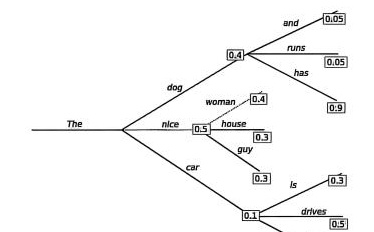
\includegraphics{images/image-0018.jpeg}
\caption{波束搜索树状示例}
\end{figure}

\textbf{Top-k 采样}：从概率最高的 \(k\) 个词中随机选择下一个词，平衡稳定性和多样性。

\[
S_k = \{x_i \mid P(x_i \mid x_1, x_2, \ldots, x_T) \mathcjk{ \mathcjk{是前} } k \mathcjk{ \mathcjk{高的}}\}
\]

\[
x_{T+1} \sim P(x_{T+1} \mid x_1, x_2, \ldots, x_T) \mathcjk{，\mathcjk{在} } S_k \mathcjk{ \mathcjk{中随机选择}}
\]

\textbf{Top-p 采样（Nucleus Sampling）}：从概率累积达到 \(p\) 的最小词集中随机选择下一个词，动态调整采样范围。

\[
S_p = \{x_i \mid \sum_{j=1}^{i} P(x_j \mid x_1, x_2, \ldots, x_T) \le p\}
\]

\[
x_{T+1} \sim P(x_{T+1} \mid x_1, x_2, \ldots, x_T) \mathcjk{，\mathcjk{在} } S_p \mathcjk{ \mathcjk{中随机选择}}
\]

下面是Top-p采样的示意图：

\begin{figure}[htbp]
\centering
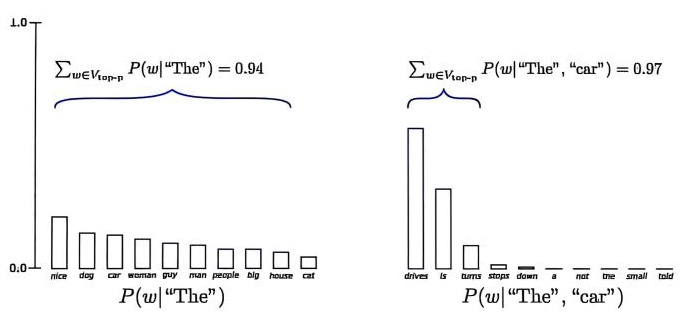
\includegraphics{images/image-0019.jpeg}
\caption{Top-p 采样分布示意图}
\end{figure}

也可以将Top-k与Top-p结合：先选K个，再从中选概率p。

\hypertarget{ux53c2ux8003ux6587ux732e-73}{%
\subsection{参考文献}\label{ux53c2ux8003ux6587ux732e-73}}

\begin{itemize}
\tightlist
\item
  《动手学大模型智能体》。
\end{itemize}

\clearpage

\hypertarget{ux540eux8badux7ec3}{%
\section{后训练}\label{ux540eux8badux7ec3}}

尽管预训练后的模型通过文本（或者还包括了其他类型的数据）学习到了海量的知识，但这样训练完毕的模型往往还不能满足人类的真实需求。大模型往往还需要经过后训练，即迁移学习（Transfer Learning）。具体地来说，就是要将一个在``源任务''（Source Task）上预训练好的模型所学到的知识，``迁移''并应用到一个新的、但相关的``目标任务''（Target Task）上。

\hypertarget{ux4e00ux4e3aux4ec0ux4e48ux8fc1ux79fbux5b66ux4e60ux5982ux6b64ux91cdux8981}{%
\subsection{一、为什么迁移学习如此重要？}\label{ux4e00ux4e3aux4ec0ux4e48ux8fc1ux79fbux5b66ux4e60ux5982ux6b64ux91cdux8981}}

迁移学习的出现是为了解决传统机器学习面临的两个核心挑战：

\begin{enumerate}
\def\labelenumi{\arabic{enumi}.}
\item
  数据稀缺问题：在许多现实世界的应用中（如医疗影像、特定物种识别），获取大量高质量的``带标签数据''是非常困难和昂贵的。
\item
  训练成本问题：从零开始（from scratch）训练一个大型深度学习模型（如图像领域的 ResNet、VGG，或 NLP 领域的 BERT、GPT）需要海量的计算资源（数周的 GPU/TPU 时间）和庞大的数据集（如 ImageNet）。
\end{enumerate}

迁移学习通过``站在巨人的肩膀上''完美地解决了这两个问题。研究机构可以先在一个通用的、海量的数据集上（如 ImageNet 包含 100 多万张通用图片）训练一个强大的``基础模型''，它已经充分学习了逐层提取图像特征的方法。当面对一个只有 1000 张 X 光片（目标任务）的特定任务时，不必从零开始训练，而是可以加载这个``基础模型''，并在此基础上针对X光片的任务进行快速、高效的训练。

\hypertarget{ux4e8cux4e24ux79cdux7b56ux7565ux7684ux6bd4ux8f83}{%
\subsection{二、两种策略的比较}\label{ux4e8cux4e24ux79cdux7b56ux7565ux7684ux6bd4ux8f83}}

\begin{enumerate}
\def\labelenumi{\arabic{enumi}.}
\tightlist
\item
  固定编码器学习（Fix-encoder learning）：将预训练模型的主体部分（即``编码器''或``Backbone''）的所有参数冻结，使其在训练中保持不变，将这个冻结的模型当作一个固定的``特征提取器''。去掉模型的原始输出层（例如，ImageNet 的 1000 类输出），换上一个为``目标任务''新设计的、小型的分类/回归``头''（通常是一个或多个全连接层），只训练这个新添加的``头''。
\end{enumerate}

适用场景：目标任务的数据集非常小，源任务和目标任务非常相似（例如，都是自然图像分类）。

\begin{enumerate}
\def\labelenumi{\arabic{enumi}.}
\setcounter{enumi}{1}
\tightlist
\item
  全量微调（Full-model tuning）：刚开始也冻结主体部分所有参数，以免过大的调整梯度摧毁预训练学到的知识；训练后期，损失对添加的``头''的梯度已经较小，解冻模型权重，并对全模型用一个极小的学习率调优。后面仍会详细介绍其原理。
\end{enumerate}

适用场景：目标任务的数据集相对充足，或源任务和目标任务有一定差异。几乎所有LLM都用这种方式进行后训练。

\begin{enumerate}
\def\labelenumi{\arabic{enumi}.}
\setcounter{enumi}{2}
\tightlist
\item
  LoRA微调（Microsoft，ICLR2022）
\end{enumerate}

（1）核心原理

LoRA基于一个核心假设：过参数化的大模型在适应特定任务时，其权重更新矩阵（W\_t+1-W\_t）具有极低的``内在秩''，设其为r（一般取4或8，大于8时输出一般不会再变优）。这也就意味着W\_t+1-W\_t中的所有向量端点都集中在一个r维空间中（只有r各基向量）。其设计思路是冻结原模型的参数W\_0（假设这是一个d\emph{k维的矩阵），训练一个r}k维的低秩矩阵A和一个d\emph{r维的低秩矩阵B，最终参数为W=W\_0+B}A。

对于基于Transformer的模型，我们一般只对W\_Q和W\_V进行微调。

（2）参数初始化

矩阵A用随机高斯分布进行初始化，矩阵B初始化为0矩阵。

如果两个都初始化为0矩阵：由链式法则，输出对A、B的梯度均为0，无法更新。

如果两个都用高斯分布初始化：A*B不是零矩阵，也就相当于把一个随机矩阵作为噪声被直接加到预训练过的权重上，破坏模型从海量数据中学到的宝贵知识。

（3）学习率设置

一般LoRA微调的学习率会高于全模型微调。因为全模型微调可以更改所有维度，必须极其谨慎；LoRA微调只能改变高维空间中的r个维度（低维流形），因此相对风险更小。

（4）针对多任务的c-LoRA

针对任务，在不同数据集上分别训练出A1\emph{B1,A2}B2,\ldots，如果直接用W=W0+A1\emph{B1+A2}B2+\ldots 效果不好，因为不同任务训练出的矩阵会互相影响。例如A1\emph{B1代表往某个方向移动5，A2}B2在该方向是4，加起来却变成了和二者都相差较大的9。为此，可采取以下方案：

正交化：让矩阵Ai\emph{Bi和Aj}Bj正交（虽然矩阵A写成m行n列，但几何上看更新模型m个n维向量的权重等价于对一个m\emph{n的长向量更新权重，正交即长向量点积为零，表示两个矩阵代表的移动在整体上互不干涉），只需要Ai}Bi所有非零元素在Aj*Bj中都强制为零，只需要Ai所有非零元素在Aj中都强制为零。

MoE架构：把经过不同方式微调得到的模型作为不同专家。

融合（取平均或加权平均）：相当于各参数取中间值或凸组合，由于损失关于参数的函数近似是凸函数，效果往往尚可。

\hypertarget{ux4e09ux76d1ux7763ux5faeux8c03}{%
\subsection{三、监督微调}\label{ux4e09ux76d1ux7763ux5faeux8c03}}

\begin{enumerate}
\def\labelenumi{\arabic{enumi}.}
\tightlist
\item
  监督微调的核心方法
\end{enumerate}

通过在海量的无标注文本上进行预训练，LLM已经具备了丰富的知识和语言能力。但它的输出是 ``你想知道什么，我就尽量拼凑出相关文字''，采用``回答问题''的语言模式的意识不强。因此，我们用一个``指令-回答对''数据集，让LLM预测回答中的token。和预训练不同的是，这里的训练是``看全部指令+回答的前t-1个token，预测回答的第t个token''。虽然模型在读指令时也做出了预测，但我们不在乎它预测得对不对。我们通过Loss Mask把指令部分的 Loss设为0。

监督微调的数据集来源可以为人工构造、蒸馏合成（用其他AI模型生成）、自我增强合成（自身生成、自我打分并完善）等，需要注意每个任务类型样本量的均衡性，以及在LLM的训练中需要多样化提问措辞。

\begin{enumerate}
\def\labelenumi{\arabic{enumi}.}
\setcounter{enumi}{1}
\tightlist
\item
  监督微调的整体步骤
\end{enumerate}

如要训练一个AI来区分狗和猫，但只有100张照片。可以找一个大型预训练模型，虽然它可能不认识你特定的猫或狗的品种，但它已经见过了数百万张图片，它已经深刻理解了底层特征（什么是边缘、角落、颜色）、中层特征（什么是纹理（如皮毛、草地）、圆形（如眼睛、轮子））、高层特征（什么是脸、腿、汽车的形状）。

（1）加载预训练模型的主体

在Keras或PyTorch框架中，这只是一行代码。例如：model = ResNet50(weights=`imagenet', include\_top=False)。其中weights=`imagenet' 告诉框架：``请加载你在ImageNet数据集上训练好的所有知识（权重）。''include\_top=False 的意思是：``把那个1000个分类的最后一层扔掉，我只想要前面强大的特征提取层。''

（2）手动添加我们自己的新层

例如：x = model.output（获取``身体''的输出），然后 predictions = Dense(2, activation=`softmax')(x)（添加一个只有2个输出的新``头部''）。这个新的 Dense(2, \ldots) 层是完全未经训练的------它的权重是随机初始化的。

（3）冻结预训练模型的主体的权重

否则，那个随机初始化的Dense(2)层会做出完全随机的、非常糟糕的猜测，训练算法（反向传播）会并试图通过一个巨大的``修正信号''（即梯度）来纠正它，破坏掉所有那些从超大型数据集上学来的预训练知识。因此我们通过一行代码，告诉模型：``嘿，`巨人身体'（比如 ResNet50 的所有层）已经很完美了，在训练时不要更新它们。把它们当作`只读'。''在Keras中，这就像 model.layers{[}i{]}.trainable = False。所有的``修正信号''只会用来训练新加入的层。

（4）解冻与精细微调

``巨人身体''从ImageNet等超大型数据集学到的知识（比如如何识别``皮毛''、``眼睛''）虽然很棒，但它们是通用知识。它们还不是专门为``区分猫和狗''而优化的。

现在，我们的新加入``头部''层已经训练好了，不会再发送混乱的信号，故可以``解冻''（unfreeze）预训练好的``巨人身体''最上面的几层（我们通常还是会保持底层如图像的``边缘/颜色''检测层冻结），然后用一个极其微小的学习率（如learning rate=0.00001）再去训练它们，让这些层``微调''自己，变得更擅长我们的特定任务。注意，这些层已经是训练有素的``专家''了。如果我们用一个常规的学习率（比如 0.001），这个``修正信号''对它们来说还是太强了，就像用大锤去修理一块精密的手表，会瞬间毁掉它们。要用一个极小的学习率，让它们在保持原有知识的基础上，稍稍``偏向''我们的任务。

\begin{enumerate}
\def\labelenumi{\arabic{enumi}.}
\setcounter{enumi}{2}
\tightlist
\item
  专家蒸馏（DeepSeek-V3.2，2025）
\end{enumerate}

专家蒸馏是监督微调与模型蒸馏（见模型压缩部分）的结合，其核心思想是：不同任务由专门的专家模型来承担学习，再将这些专家的能力汇聚到统一的大模型中。

团队首先从同一个DeepSeek-V3.2基础检查点出发，为数学、编程、逻辑推理、通用智能体、智能体编程和智能体搜索等六类专业任务分别训练专属模型，这些模型拥有思考模式和直接作答模式两类数据，并利用大规模RL进行强化，以保证每个专家在自己的领域达到高水准。

随后，这些专家会负责生成高质量的领域数据，用来训练一个统一的大模型。实验表明，用专家数据蒸馏出来的大模型性能已经非常接近各个专家本身，再辅以后续的RL微调，残余的差距也可以基本消除。

\hypertarget{ux56dbux5f3aux5316ux5faeux8c03}{%
\subsection{四、强化微调}\label{ux56dbux5f3aux5316ux5faeux8c03}}

在预训练阶段，模型通过``让预测的Next token接近实际文本''的方式对训练数据进行自监督学习；在监督微调（SFT）阶段，模型通过``让回答接近人类标注''的方式模仿训练数据中人类的回答模式。

这两种方法共同的缺陷是，模型只能像鹦鹉学舌一样，学习数据里的逻辑，泛化能力弱。而且，有些任务人类容易评价，但难直接给出解答，比如人类很容易判断两个笑话哪个更好笑，但很难自己写出一个极好的笑话。

强化学习可以解决这个问题。我们不需要手把手教它每一个字怎么写，只需要给模型的答案评分，模型就能自主探索，找到通往高分的路径，在这个过程中模型的方法甚至能达到超越人类的水平。AlphaGo就是如此。

\begin{enumerate}
\def\labelenumi{\arabic{enumi}.}
\tightlist
\item
  LLM与马尔可夫决策过程
\end{enumerate}

对于LLM，我们可以将其每生成一个token之后的状态视为马尔可夫决策模型中的``状态''，将生成一个token（设为x\_t）视为一种``动作''（在智能体中，也可以是函数调用、API 执行或代码片段输出），这个过程就是从状态（x\_1,\ldots,x\_t-1）到（x\_1,\ldots,x\_t）的状态转移，``策略''就是选择各个token的概率。奖励函数依据输出结果是否正确、输出是否规范、程序运行是否成功等确定。

在回答同一个特定问题时，由于LLM每次生成token（每走一个动作）都具有概率上的随机性，因此它会生成很多不同回答。我们取N个回答，对应的就是强化学习中采样N条从起点到终点的完整路径（可用于蒙特卡洛估计，即用频率估计概率）。

\begin{enumerate}
\def\labelenumi{\arabic{enumi}.}
\setcounter{enumi}{1}
\tightlist
\item
  强化微调的概念
\end{enumerate}

在LLM诞生以前，人们在游戏、下棋等方面运用RL进行了许多有益的尝试，但这些基于RL的模型都难以达到真正意义上的通用智能。LLM诞生后，人们发现经过海量数据预训练的LLM往往具有很强的语义理解和模式匹配能力，但其本质仍是基于概率的``压缩''和``模仿''，模型无法获得超越训练数据的能力。而RL只根据目标，在与环境的互动中进行探索和优化，它能生成``超越''已有模式的方法（如AlphaGo的``第37手''），但传统RL一旦扩展到通用问题就难以收敛，重要原因就是没有LLM作为先验。

于是新的范式产生了：在已经具有丰富知识和理解能力的LLM基础上运用RL进行微调，扩展其能力边界，如推理能力等。相对于传统意义上的强化学习，强化微调往往动作空间更大，样本量更小。

强化微调具体又分为RLHF（基于人类反馈的强化学习）和针对推理等能力的强化学习。实现前者需要我们对符合人类喜好的回答打高分，但人类反馈往往昂贵且低效，因此我们往往训练一个奖励模型，让它学会模仿人类的喜好来打分，用这个奖励模型对待训练的模型打分。实现后者也需要有明确的评分标准或较强的评分模型，比如用数学题或编程题训练模型的推理能力，用结果是否正确等作为奖励信号。

强化微调的具体实现算法可见强化微调部分介绍。

\begin{enumerate}
\def\labelenumi{\arabic{enumi}.}
\setcounter{enumi}{2}
\tightlist
\item
  RLHF（基于人类反馈的强化学习）
\end{enumerate}

经过了监督微调以及针对推理的强化微调之后，模型极其聪明，但模型可能会比较难用，比如出现中英文夹杂、说话重复、或者语气很冲等情况，因为它只管把题做对，不管人类看着舒不舒服；还可能存在安全性问题，因为它的价值观可能未和人类对齐。

强化学习中，``奖励''非常重要，但我们不可能让人类给所有训练回答打分。因此，我们用一个问题，让模型生成两个（或多个）回答，让人类给其优劣排名，通过回答-排名数据来训练奖励模型，鼓励奖励模型给更优的回答给出高分，反之亦然。

\begin{enumerate}
\def\labelenumi{\arabic{enumi}.}
\setcounter{enumi}{3}
\tightlist
\item
  RLVR（Reinforcement Learning from Verifiable Rewards，基于可验证奖励的强化学习）
\end{enumerate}

在强化微调中，确定一个合适的奖励至关重要，这决定了问题能不能被RL正确地建模。RLHF基于人类反馈给模型奖励信号，用这个奖励信号对模型进行强化学习训练。但人类评审员也是人，他们很难在几秒钟内判断一段500行的Python代码是否真的没有Bug，或者一个复杂的数学证明是否严丝合缝。于是，模型学会了走捷径：写出漂亮但错误的代码，编造听起来很有道理的废话，以``骗取''较高的奖励分数。这就是所谓的Reward Hacking问题，即由于奖励函数设置的局限性，奖励函数的值最大有时并不代表最能达到我们想要的目的，模型可能获得了很高的奖励，却在真实世界的任务中表现不佳。

基于可验证奖励的强化学习即运用数学题答案、编程题输出结果等客观、可验证的结果作为奖励信号，有效避免了Reward Hacking问题。模型在训练过程中自行探索最优的路径，最终获得正确答案。值得一提的是，这个探索出的路径甚至可能是人类从未发明过的，也就意味着通过RLVR，我们有可能让模型在对应任务上取得超出人类水平的表现。

\hypertarget{ux53c2ux8003ux6587ux732e-74}{%
\subsection{参考文献}\label{ux53c2ux8003ux6587ux732e-74}}

\begin{itemize}
\tightlist
\item
  Hu, E. J., Shen, Y., Wallis, P., et al.~(2022). \href{https://arxiv.org/abs/2106.09685}{LoRA: Low-Rank Adaptation of Large Language Models}. ICLR 2022.
\item
  DeepSeek-AI. (2025). \href{https://arxiv.org/abs/2512.02556}{DeepSeek-V3.2: Pushing the Frontier of Open Large Language Models}. arXiv:2512.02556.
\item
  Silver, D., Huang, A., Maddison, C. J., et al.~(2016). \href{https://www.nature.com/articles/nature16961}{Mastering the game of Go with deep neural networks and tree search}. Nature.
\item
  Ouyang, L., Wu, J., Jiang, X., et al.~(2022). \href{https://arxiv.org/abs/2203.02155}{Training Language Models to Follow Instructions with Human Feedback}. NeurIPS 2022.
\item
  DeepSeek-AI. (2025). \href{https://arxiv.org/abs/2501.12948}{DeepSeek-R1: Incentivizing Reasoning Capability in LLMs via Reinforcement Learning}. arXiv:2501.12948.
\end{itemize}

\clearpage

\hypertarget{ux6df7ux5408ux4e13ux5bb6ux6a21ux5757}{%
\section{混合专家模块}\label{ux6df7ux5408ux4e13ux5bb6ux6a21ux5757}}

在经过Attention层后，不同token之间进行了充分的信息交换和融合。随后，由前馈神经网络（FFN）进行加工和处理。FFN一般为带有门控的GLU网络：

常见的 SwiGLU FFN 可以写为：

\[
FFN_{\mathrm{SwiGLU}}(x) = (\sigma(xW_1) \otimes (xV))W_2
\]

其中：

\begin{itemize}
\tightlist
\item
  \(W_1\) 是门控分支（Gate）的权重矩阵，\(\sigma\) 是激活函数（例如 Swish 或 SiLU）。
\item
  \(V\) 是值分支（Value）的权重矩阵。
\item
  \(\otimes\) 表示逐元素相乘（Hadamard product）。
\item
  \(W_2\) 是最终输出投影的权重矩阵。
\end{itemize}

算法工作流如下：

\begin{enumerate}
\def\labelenumi{\arabic{enumi}.}
\tightlist
\item
  \textbf{门控分支投影（Gate Projection）}：将输入 \(x\) 乘以 \(W_1\)，映射到内部隐藏维度 \(d_{ff}'\)，并经过激活函数 \(\sigma\) 处理，生成用于控制信息流动的``门限''。
\item
  \textbf{值分支投影（Value Projection）}：并行地将输入 \(x\) 乘以矩阵 \(V\)，映射到相同的隐藏维度 \(d_{ff}'\)，这个分支保持线性状态（不加激活函数）。
\item
  \textbf{门控融合（Element-wise Multiplication）}：将步骤 1 生成的非线性门控信号与步骤 2 生成的线性值信号逐元素相乘。这一步赋予了网络动态过滤特征的能力，相当于让输入自己决定哪些特征应该被保留或放大。
\item
  \textbf{降维投影（Down-projection）}：将融合后的向量乘以 \(W_2\)，重新映射回原始维度 \(d_{model}\)。
\end{enumerate}

实践中，FFN往往占据了较大的参数规模。

为了在扩大参数规模（千亿/万亿级）的同时保持高效的推理速度，Deepseek、Gemini等模型均采用了MoE架构代替全连接层。在每一个Transformer Block中，Attention层之后都接一个MoE层作为信息加工和处理模块。MoE层根据内容的特征，把每个token都分配给一部分``专家''有针对性地加工处理，而不需要激活其他``专家''的参数，增强前向计算的稀疏性。

\hypertarget{ux4e00ux5c06ux8f93ux5165ux5206ux914dux7ed9ux4e13ux5bb6}{%
\subsection{一、将输入分配给专家}\label{ux4e00ux5c06ux8f93ux5165ux5206ux914dux7ed9ux4e13ux5bb6}}

\hypertarget{ux7b26ux53f7ux5b9aux4e49notation}{%
\subsubsection{1. 符号定义（Notation）}\label{ux7b26ux53f7ux5b9aux4e49notation}}

设输入序列包含 \(T\) 个 Token（\(T=\text{Batch Size} \times \text{Sequence Length}\)），隐藏层维度为 \(d\)。

\begin{itemize}
\tightlist
\item
  \textbf{输入张量}：\(X \in \mathbb{R}^{T \times d}\)。第 \(t\) 个 Token 表示为行向量 \(x_t\)。
\item
  \textbf{专家集合}：\(\mathcal{E}=\{E_1,E_2,\ldots,E_N\}\)，共有 \(N\) 个专家网络。
\item
  \textbf{专家函数}：\(E_i(x): \mathbb{R}^d \to \mathbb{R}^d\)，即第 \(i\) 个前馈神经网络。
\item
  \textbf{门控参数}：\(W_g \in \mathbb{R}^{d \times N}\)，用于计算路由分数的权重矩阵。
\end{itemize}

\hypertarget{ux95e8ux63a7ux4e0eux7a00ux758fux8defux7531gating-sparse-routing}{%
\subsubsection{2. 门控与稀疏路由（Gating \& Sparse Routing）}\label{ux95e8ux63a7ux4e0eux7a00ux758fux8defux7531gating-sparse-routing}}

这是 MoE 的决策阶段，决定每个 Token 发送给哪 \(k\) 个专家。

\hypertarget{ux539fux59cbux5206ux6570ux8ba1ux7b97raw-logits}{%
\paragraph{2.1 原始分数计算（Raw Logits）}\label{ux539fux59cbux5206ux6570ux8ba1ux7b97raw-logits}}

首先计算输入 \(X\) 对应每个专家的原始匹配分数矩阵 \(H \in \mathbb{R}^{T \times N}\)：

\[
H = XW_g
\]

\hypertarget{top-k-ux7a00ux758fux5316top-k-sparsification}{%
\paragraph{2.2 Top-k 稀疏化（Top-k Sparsification）}\label{top-k-ux7a00ux758fux5316top-k-sparsification}}

为了实现稀疏计算，我们只保留每行中最大的 \(k\) 个值。定义算子 \(\mathrm{TopK}(v,k)\)，对于向量 \(v\)，保留前 \(k\) 大的元素，其余置为 \(-\infty\)。

对于第 \(t\) 个 Token 的分数向量 \(h_t\)（矩阵 \(H\) 的第 \(t\) 行）：

\[
\tilde{h}_t = \mathrm{TopK}(h_t,k)
\]

\hypertarget{ux95e8ux63a7ux6743ux91cdgating-weights}{%
\paragraph{2.3 门控权重（Gating Weights）}\label{ux95e8ux63a7ux6743ux91cdgating-weights}}

对稀疏化后的分数进行 Softmax 归一化，得到最终的门控权重矩阵 \(G \in \mathbb{R}^{T \times N}\)：

\[
G = \mathrm{Softmax}(\tilde{H})
\]

注意：\(G\) 是一个行稀疏矩阵，每一行 \(G_t\) 只有 \(k\) 个非零元素。这些非零元素即为该 Token 分配给对应专家的权重。

\hypertarget{ux8c03ux5ea6ux4e0eux4e13ux5bb6ux8ba1ux7b97dispatch-expert-computation}{%
\subsubsection{3. 调度与专家计算（Dispatch \& Expert Computation）}\label{ux8c03ux5ea6ux4e0eux4e13ux5bb6ux8ba1ux7b97dispatch-expert-computation}}

在实际的矩阵并行计算中，我们不通过循环处理，而是通过索引掩码或选择矩阵来实现。

\hypertarget{ux5b9aux4e49ux9009ux62e9ux77e9ux9635selection-matrix}{%
\paragraph{3.1 定义选择矩阵（Selection Matrix）}\label{ux5b9aux4e49ux9009ux62e9ux77e9ux9635selection-matrix}}

对于第 \(i\) 个专家，定义一个二值选择矩阵 \(M_i \in \{0,1\}^{C_i \times T}\)，其中 \(C_i\) 是分配给专家 \(i\) 的 Token 总数（即容量）。如果输入中的第 \(t\) 个 Token 被分配给了专家 \(i\)，则 \(M_i\) 中对应行和列的位置为 1。

\hypertarget{ux4e13ux5bb6ux8f93ux5165ux6295ux5f71dispatch}{%
\paragraph{3.2 专家输入投影（Dispatch）}\label{ux4e13ux5bb6ux8f93ux5165ux6295ux5f71dispatch}}

通过矩阵乘法，将分散在 Batch 中的 Token 聚集到专家 \(i\) 的输入缓冲区 \(X_i \in \mathbb{R}^{C_i \times d}\)：

\[
X_i = M_iX
\]

这里 \(X_i\) 矩阵的第 \(m\) 行第 \(k\) 列，代表第 \(i\) 个专家输入向量第 \(m\) 个 token 的第 \(k\) 个维度（Embedding 空间是 \(d\) 维的）。由于它由 \(M_i\) 矩阵的第 \(m\) 行（第 \(i\) 个专家输入的第 \(m\) 个 token 是总序列的第 \(n\) 个 token，则该行第 \(n\) 列为 \(1\)，其他列为 \(0\)）和 \(X\) 矩阵的第 \(k\) 列（各个 token 的第 \(k\) 列数值）点乘得到，因此它实际上是``从总输入矩阵中提取本专家输入矩阵''，从而略掉不属于本专家处理的内容。

\hypertarget{ux4e13ux5bb6ux5904ux7406processing}{%
\paragraph{3.3 专家处理（Processing）}\label{ux4e13ux5bb6ux5904ux7406processing}}

第 \(i\) 个专家对其专属的输入数据进行计算，得到输出 \(Z_i \in \mathbb{R}^{C_i \times d}\)：

\[
Z_i = E_i(X_i)
\]

\hypertarget{ux4e8cux805aux5408ux4e13ux5bb6ux7684ux8f93ux51fa}{%
\subsection{二、聚合专家的输出}\label{ux4e8cux805aux5408ux4e13ux5bb6ux7684ux8f93ux51fa}}

\hypertarget{ux52a0ux6743ux805aux5408weighted-combination}{%
\subsubsection{4. 加权聚合（Weighted Combination）}\label{ux52a0ux6743ux805aux5408weighted-combination}}

最后一步是将各个专家的计算结果 \(Z_i\) 发送回原来的位置，并乘以门控权重。

\hypertarget{ux6743ux91cdux5411ux91cfux5316}{%
\paragraph{4.1 权重向量化}\label{ux6743ux91cdux5411ux91cfux5316}}

对于专家 \(i\)，其对应的门控权重向量 \(g_i \in \mathbb{R}^{C_i}\) 是矩阵 \(G\) 第 \(i\) 列中所有非零值的集合：

\[
g_i = M_iG_{:,i}
\]

MoE 层的总输出 \(Y \in \mathbb{R}^{T \times d}\) 由所有专家的结果经过 \(M_i^T\)（起到 Scatter 作用）还原位置后叠加而成：

\[
Y = \sum_{i=1}^{N} M_i^T(\mathrm{diag}(g_i) \cdot Z_i)
\]

如果从单个 Token \(x\) 的角度看，这个过程等价于更直观的求和公式：

\[
y = \sum_{i \in \mathcal{T}} G(x)_iE_i(x)
\]

其中 \(\mathcal{T}\) 是被选中的 Top-k 专家索引集合。

具体解释：

\begin{enumerate}
\def\labelenumi{\arabic{enumi}.}
\tightlist
\item
  \(g_i=M_iG_{:,i}\)：预处理步骤，将各专家的权重向量``聚合''以适配后续矩阵乘法维度
\end{enumerate}

\(M_i\) 是前面所述的二值选择矩阵，形状为 \(C_i\times T\)（\(C_i\) 是选中专家 \(i\) 的 Token 数量）。它是一个稀疏的二值矩阵（只有 \(0\) 和 \(1\)），每一行只有一个 \(1\)，代表``我选中的第 \(k\) 个 Token 在原始 Batch 的第几行''。

\(G_{:,i}\) 表示 \(G\) 的第 \(i\) 列，这是一个长度为 \(T\)（序列中 Token 总数）的列向量。它代表了 Batch 中所有 Token 对专家 \(i\) 的打分（权重），这是一个稀疏的向量，里面有很多 \(0\)。在这个矩阵乘法后，就变成了长度为 \(C_i\)（选择了专家 \(i\) 的 Token），相当于把 \(0\) 全部去掉之后拼接起来。

这个操作的核心目的是让权重向量能在后续矩阵乘法中维度匹配（\(Z_i\) 是 \(C_i\times d\) 矩阵）。

举个例子：

假设 Batch Size \(T=4\)，专家 \(i=1\)。Token 1 和 Token 3 选中了专家 1，Token 2 和 Token 4 没选中。

\begin{enumerate}
\def\labelenumi{\arabic{enumi}.}
\tightlist
\item
  全局权重列向量 \(G_{:,1}\) 记录所有 Token 对专家 1 的权重：
\end{enumerate}

\[
G_{:,1} =
\begin{pmatrix}
0.9 \\
0 \\
0.8 \\
0
\end{pmatrix}
\]

其中 Token 1 的权重为 0.9（选中），Token 2 的权重为 0（没选中），Token 3 的权重为 0.8（选中），Token 4 的权重为 0（没选中）。

\begin{enumerate}
\def\labelenumi{\arabic{enumi}.}
\setcounter{enumi}{1}
\tightlist
\item
  选择矩阵 \(M_1\) 表示专家 1 只负责处理第 1 个和第 3 个 Token，所以 \(M_1\) 是 \(2 \times 4\) 矩阵：
\end{enumerate}

\[
M_1 =
\begin{pmatrix}
1 & 0 & 0 & 0 \\
0 & 0 & 1 & 0
\end{pmatrix}
\]

\begin{itemize}
\tightlist
\item
  第一行 \([1,0,0,0]\)：提取原来的第 1 个元素。
\item
  第二行 \([0,0,1,0]\)：提取原来的第 3 个元素。
\end{itemize}

\begin{enumerate}
\def\labelenumi{\arabic{enumi}.}
\setcounter{enumi}{2}
\tightlist
\item
  计算结果 \(g_1\) 执行矩阵乘法 \(M_1 \times G_{:,1}\)：
\end{enumerate}

\[
g_1 =
\begin{pmatrix}
1 & 0 & 0 & 0 \\
0 & 0 & 1 & 0
\end{pmatrix}
\cdot
\begin{pmatrix}
0.9 \\
0 \\
0.8 \\
0
\end{pmatrix}
=
\begin{pmatrix}
0.9 \\
0.8
\end{pmatrix}
\]

也可以把它看作一个过滤筛查的过程：

\begin{enumerate}
\def\labelenumi{\arabic{enumi}.}
\item
  \(G_{:,i}\) 拿着一张长长的清单，上面写着 Batch 里 1000 个 Token 对专家 \(i\) 的关注度。
\item
  \(M_i\) 拿着一张``准入名单''，上面只写着 50 个真正进入专家 \(i\) 房间的 Token 的 ID。
\item
  乘法操作：\(M_i\) 将这 50 个 Token 对应的关注度（权重）从 \(G_{:,i}\) 的长清单中抠出来，按顺序排成一个新的短向量 \(g_i\)。
\item
  \(\mathrm{diag}(g_i)Z_i\)：
\end{enumerate}

物理意义：专家处理完数据后，我们不能直接使用结果，必须根据门控网络（Router）的``信任程度''对结果进行缩放。如果门控网络给专家 \(i\) 的打分很高（例如 \(0.9\)），那么 \(Z_i\) 的特征就保留大部分；如果打分很低（例如 \(0.1\)），特征就被削弱。

数学操作：

\begin{itemize}
\tightlist
\item
  \(g_i\) 是一个长度为 \(C_i\) 的向量。
\item
  \(\mathrm{diag}(g_i)\) 将其构造为一个 \(C_i \times C_i\) 的对角矩阵。
\item
  与 \(Z_i\)（\(C_i \times d\)）相乘，本质上是行与行之间的标量乘法（Broadcast multiplication），即第 \(j\) 个样本的输出向量乘以第 \(j\) 个权重标量。
\end{itemize}

\begin{enumerate}
\def\labelenumi{\arabic{enumi}.}
\setcounter{enumi}{2}
\tightlist
\item
  乘 \(M_i^T\)：把行数从该专家处理的 token 数散射还原到整个序列的 token 数，以便后续相加
\end{enumerate}

假设总共有 4 个 Token（\(T=4\)），专家 \(E_1\) 负责处理第 1 个和第 3 个 Token（\(C_1=2\)）。

Gather 阶段（\(X_i=M_iX\)）：\(M_i\) 是一个 \(2 \times 4\) 的矩阵，它把第 1、3 行``吸''出来，变成紧凑的 \(2 \times d\) 矩阵送给专家。

\[
M_i =
\begin{pmatrix}
1 & 0 & 0 & 0 \\
0 & 0 & 1 & 0
\end{pmatrix}
\]

Scatter 阶段（\(M_i^T\)）：现在专家算完了，得到结果 \(Z_i'\)（加权后的 \(2 \times d\) 矩阵）。我们需要把它放回原来的 4 行结构中。\(M_i^T\) 是 \(M_i\) 的转置，形状为 \(4 \times 2\)：

\[
M_i^T =
\begin{pmatrix}
1 & 0 \\
0 & 0 \\
0 & 1 \\
0 & 0
\end{pmatrix}
\]

当我们将 \(M_i^T\) 乘以 \(2 \times d\) 的结果矩阵时：

\[
\begin{pmatrix}
1 & 0 \\
0 & 0 \\
0 & 1 \\
0 & 0
\end{pmatrix}
\cdot
\begin{pmatrix}
\mathrm{Row}_1 \\
\mathrm{Row}_3
\end{pmatrix}
=
\begin{pmatrix}
\mathrm{Row}_1 \\
0 \\
\mathrm{Row}_3 \\
0
\end{pmatrix}
\]

\begin{enumerate}
\def\labelenumi{\arabic{enumi}.}
\setcounter{enumi}{3}
\tightlist
\item
  求和：各专家输出矩阵相加，得到最终输出
\end{enumerate}

\hypertarget{ux4e09ux8d1fux8f7dux5747ux8861ux635fux5931}{%
\subsection{三、负载均衡损失}\label{ux4e09ux8d1fux8f7dux5747ux8861ux635fux5931}}

为了防止``马太效应''（即少数专家处理所有数据），我们需要在训练目标函数中加入辅助项。

定义两个概率分布向量：

\begin{enumerate}
\def\labelenumi{\arabic{enumi}.}
\tightlist
\item
  重要性分布（Importance Vector，\(\Psi\)）：门控网络预测的累积概率质量，即模型``想''怎么分。
\end{enumerate}

\[
\Psi_i = \frac{1}{T}\sum_{t=1}^{T}\mathrm{Softmax}(h_t)_i
\]

\begin{enumerate}
\def\labelenumi{\arabic{enumi}.}
\setcounter{enumi}{1}
\tightlist
\item
  负载分布（Load Vector，\(\Phi\)）：实际产生的离散分配决策，即实际怎么分。
\end{enumerate}

\[
\Phi_i = \frac{1}{T}\sum_{t=1}^{T}\mathbf{1}\left(i \in \mathrm{Indices}(\mathrm{TopK}(h_t,k))\right)
\]

\begin{enumerate}
\def\labelenumi{\arabic{enumi}.}
\setcounter{enumi}{2}
\tightlist
\item
  损失函数：最小化这两个向量的点积，以鼓励均匀分布（Uniform Distribution）。
\end{enumerate}

\[
\mathcal{L}_{aux} = N\sum_{i=1}^{N}\Psi_i \cdot \Phi_i
\]

\begin{itemize}
\tightlist
\item
  系数 \(N\) 是为了归一化，使得理想均匀分布下的 Loss 为 1。
\item
  总损失函数为：\(\mathcal{L}_{total}=\mathcal{L}_{task}+\alpha\mathcal{L}_{aux}\)。
\end{itemize}

此外还可以在路由分数计算中引入动态偏置：

\[
\mathrm{RoutingScore}=\mathrm{Softmax}(W_{gate}\cdot x+b_{dynamic})
\]

\hypertarget{ux56dbdeepseekux5bf9moeux7684ux521bux65b0}{%
\subsection{四、DeepSeek对MoE的创新}\label{ux56dbdeepseekux5bf9moeux7684ux521bux65b0}}

DeepSeek不是MoE的发明者，但做了非常重要的架构微创新（Micro-Innovation），极大地提升了MoE的效率。

\begin{enumerate}
\def\labelenumi{\arabic{enumi}.}
\tightlist
\item
  细粒度专家（Fine-Grained Experts）
\end{enumerate}

传统MoE的专家很大且数量少（比如 8 个大专家）。DeepSeek将专家切得更碎（比如 64 个小专家），每次激活更多的小专家。

数学直觉：粒度越细，知识组合的灵活性越高。

\begin{enumerate}
\def\labelenumi{\arabic{enumi}.}
\setcounter{enumi}{1}
\tightlist
\item
  共享专家隔离
\end{enumerate}

这是DeepSeek最核心的贡献。

传统MoE问题：有些知识是通用的（比如语法结构、基础逻辑）。在传统MoE中，这些通用知识被迫重复存储在每一个专家里，浪费参数。

DeepSeek方案在数学表达上，输出公式变成了：

\[
y=\sum_{i\in \mathrm{TopK}}G_i(x)E_i(x)+E_{shared}(x)
\]

\begin{itemize}
\tightlist
\item
  \(E_{shared}(x)\)：是一个总是被激活的专家，专门负责存储通用知识。
\item
  \(E_i(x)\)：路由专家只负责存储``细分领域的独有知识''。
\end{itemize}

\hypertarget{ux4e94top-kux64cdux4f5cux7684ux4e0dux53efux5bfcux6027ux53caux89e3ux51b3ux65b9ux6848}{%
\subsection{五、Top-K操作的不可导性及解决方案}\label{ux4e94top-kux64cdux4f5cux7684ux4e0dux53efux5bfcux6027ux53caux89e3ux51b3ux65b9ux6848}}

\begin{enumerate}
\def\labelenumi{\arabic{enumi}.}
\tightlist
\item
  受害者：路由网络（The Router）
\end{enumerate}

路由网络（参数为 \(W_r\)）是那个负责做``多选题''的角色。它的任务是：对于输入 \(x\)，我应该从几百个专家里选哪 \(K\) 个？

为什么它是受害者？

Top-K 操作本质上是一个阶跃函数（Step Function）。

\begin{itemize}
\tightlist
\item
  输入：路由分值（logits）。
\item
  输出：几个离散的索引（比如 \texttt{\{Expert\ 5,\ Expert\ 9\}}）。
\end{itemize}

问题场景：假设现在的 Loss 很高，我们希望通过梯度下降告诉 Router：``你选错了，刚才不应该选 Expert 5，应该选 Expert 7！''

但是在数学上，Top-K 造成了梯度消失（Zero Gradient）：

\begin{enumerate}
\def\labelenumi{\arabic{enumi}.}
\tightlist
\item
  如果我们微小地改变一点点路由参数 \(W_r\)，路由分值会发生微小变化（例如 Expert 5 的分值从 0.8 变到 0.801，Expert 7 的分值从 0.79 变到 0.791）。
\item
  然而，这种微小的变化不足以改变 Top-K 的排序结果（Top-K 依然选 Expert 5）。
\item
  因为结果没变，Loss 也没变。
\item
  结论：Loss 对 \(W_r\) 的导数为 0。
\end{enumerate}

后果：如果没有补救措施（如 DeepSeek 采用的加权求和 \(g_i \cdot E_i\)），Router 根本无法学习。它会随机初始化成什么样，就永远停留在什么样，因为它感觉不到任何``改变参数能降低 Loss''的反馈。

\begin{enumerate}
\def\labelenumi{\arabic{enumi}.}
\setcounter{enumi}{1}
\tightlist
\item
  幸存者：专家网络（The Experts）
\end{enumerate}

专家网络（参数为 \(W_e\)）是负责干活的执行者。

为什么它不受影响？

\begin{itemize}
\tightlist
\item
  专家本身不在乎``由于什么决策逻辑''被选中。
\item
  只要它被选中了，数据流就会进来。
\item
  只要数据流进来了，它算出的结果就会参与最终 Loss 的计算。
\item
  只要参与了计算，梯度就会顺着数据流反向传回来。
\end{itemize}

对于专家来说，Top-K 只是一个开关（Mask）。

\begin{itemize}
\tightlist
\item
  开关开了（被选中）：我就正常训练，更新参数。
\item
  开关没开（没被选中）：我就休息，参数不变。
\end{itemize}

Top-K 的不可导性没有阻断``Loss → 专家输出 → 专家权重''这条路径，它只是阻断了``Loss → 选择逻辑 → 路由权重''这条路径。

\begin{enumerate}
\def\labelenumi{\arabic{enumi}.}
\setcounter{enumi}{2}
\tightlist
\item
  DeepSeek 是如何``救活''路由网络的？
\end{enumerate}

既然 Top-K 让 Router 无法通过``改变选择''来学习，DeepSeek（以及现代 MoE）就通过\textbf{``改变幅度''}来让它学习。

回顾公式：

\[
y=\sum_{i\in T}g_i\cdot E_i(x)
\]

Router 的梯度回传路径变成了：

\[
\mathrm{Loss}\rightarrow y\rightarrow g_i\;(\mathrm{Softmax\ Probability})\rightarrow \mathrm{Logits}\rightarrow W_r
\]

这个 trick 的精髓在于：模型虽然无法直接告诉 Router``这就把 Expert 5 换成 Expert 7''（这是离散跳跃），但它可以告诉 Router：

``嘿，Expert 5 刚才的表现不错，请增大它的权重 \(g_5\)（让它更重要）。''或者``Expert 9 刚才搞砸了，请减小它的权重 \(g_9\)。''

通过不断调整连续的权重 \(g_i\)，如果某个未被选中的专家（比如 Expert 7）的潜在分值慢慢被推高，最终超过了 Top-K 的阈值，它就会在某一时刻``突然''被选中。Router 就是通过这种``曲线救国''的方式，利用连续的权重梯度，最终实现了离散选择的优化。

\hypertarget{ux53c2ux8003ux6587ux732e-75}{%
\subsection{参考文献}\label{ux53c2ux8003ux6587ux732e-75}}

\begin{itemize}
\tightlist
\item
  Jacobs, R. A., Jordan, M. I., Nowlan, S. J., \& Hinton, G. E. (1991). \href{https://doi.org/10.1162/neco.1991.3.1.79}{Adaptive Mixtures of Local Experts}. Neural Computation.
\item
  Dai, D., Deng, C., Zhao, C., et al.~(2024). \href{https://arxiv.org/abs/2401.06066}{DeepSeekMoE: Towards Ultimate Expert Specialization in Mixture-of-Experts Language Models}. arXiv:2401.06066.
\item
  DeepSeek-AI. (2024). \href{https://arxiv.org/abs/2412.19437}{DeepSeek-V3 Technical Report}. arXiv:2412.19437.
\end{itemize}

\clearpage

\hypertarget{ux591aux6a21ux6001ux5927ux8bedux8a00ux6a21ux578b}{%
\section{多模态大语言模型}\label{ux591aux6a21ux6001ux5927ux8bedux8a00ux6a21ux578b}}

\hypertarget{ux4e00ux4ee5ux6587ux672cux4e3aux4ecbux8d28ux7684ux591aux6a21ux6001ux611fux77e5}{%
\subsection{一、以文本为介质的多模态感知}\label{ux4e00ux4ee5ux6587ux672cux4e3aux4ecbux8d28ux7684ux591aux6a21ux6001ux611fux77e5}}

\hypertarget{ux57faux672cux601dux60f3}{%
\subsubsection{1. 基本思想}\label{ux57faux672cux601dux60f3}}

这种方式先由感知模型统一将图片、音频等转为语言（视频隔一定时间采样帧，转为图片+音频）。例如，独立训练（而非在LLM整体中端到端训练）一个已经预训练好的视觉Encoder，由于视觉Encoder嵌入空间和语言模型嵌入空间不一致，输出需要经过一个适配器后，再以具有语言意义、可以直接输入纯语言模型的token流的形式交给LLM处理。

这样的问题在于，一维语言难以描述高维细节，即适配器转化时存在信息损失。此外，模型整体也无法端到端优化。

\hypertarget{ux89c6ux89c9-encoderux4ee5-clip-ux4e3aux4f8b}{%
\subsubsection{2. 视觉 Encoder：以 CLIP 为例}\label{ux89c6ux89c9-encoderux4ee5-clip-ux4e3aux4f8b}}

输入图像被划分为固定大小的方格网格（通常为32×32或16×16像素），每个patch被展平为向量，转化为视觉token，经过多头自注意力层，得到图像的编码向量序列。

视觉Encoder通过``对比''来学习。模型被训练来``拉近''匹配的（正）样本对，同时``推远''不匹配的（负）样本对。如模型获取（图像，文本）对，图像和它对应的文本匹配时构成一个``正样本对''，不匹配时构成``负样本对''。给定一个 batch 的图像-文本对 \((I_1,T_1),(I_2,T_2),\ldots,(I_n,T_n)\)，模型学习的目标是最大化匹配对 \((I_i,T_i)\) 的相似度得分，最小化 \(s(I_i,T_j)\) 的相似度得分（\(j\ne i\)），要区分哪些图文是配对的，哪些不是（监督信号直接来源于数据本身，\((I_i,T_i)\) 是匹配的，其他随机组合的图文对 \((I_i,T_j)\) 被认为是大概率不匹配的）。

损失函数为InfoNCE。假设我们有：1 个``锚点''（Anchor）样本，记为 \(q\)（Query，查询）；1 个``正样本''（Positive），记为 \(k^+\)（Key，与 \(q\) 匹配的键）；\(N\) 个``负样本''（Negatives），记为 \(k_1^-,\ldots,k_N^-\)（与 \(q\) 不匹配的键），我们希望 \(q\) 与 \(k^+\) 的相似度远大于 \(q\) 与所有 \(k_i^-\) 的相似度。

InfoNCE 损失函数（针对单个 \(q\)）的表达式如下：

\[
\mathcal{L}_q=-\log \frac{\exp(\mathrm{sim}(q,k^+)/\tau)}
{\exp(\mathrm{sim}(q,k^+)/\tau)+\sum_{i=1}^{N}\exp(\mathrm{sim}(q,k_i^-)/\tau)}
\]

\(\mathrm{sim}(a,b)\)：相似度函数。通常使用余弦相似度或点积。

\(\tau\)：温度系数。这是一个超参数，后续会解释。

分式项：

\[
\frac{\exp(\mathrm{sim}(q,k^+)/\tau)}
{\exp(\mathrm{sim}(q,k^+)/\tau)+\sum_i\exp(\mathrm{sim}(q,k_i^-)/\tau)}
\]

表示运用Softmax回归，将 \(q\) 与正样本匹配的得分除以 \(q\) 与``所有候选样本''（1 个正，\(N\) 个负）匹配的总得分，得到在给定 \(q\) 和 \(N+1\) 个候选样本的情况下，模型认为 \(k^+\) 是``正确匹配''（即正样本）的预测概率。我们的目标是让这个概率趋近于 1。

\(-\log\)：交叉熵损失 (Cross-Entropy Loss)，假设我们的``真实标签''是一个one-hot编码 \([1,0,0,\ldots,0]\)（即第一个样本 \(k^+\) 是正样本，其他都是负样本），Softmax 的输出就是模型预测的概率分布（例如 \([0.9,0.05,0.03,\ldots]\)），对这个 \(N+1\) 类的分类问题取交叉熵损失，就得到了上述 InfoNCE 公式。

InfoNCE 损失就是将``对比学习''问题（拉近/推远）转化为了一个 \(N+1\) 选 1 的``分类问题''，并使用标准的交叉熵损失函数来优化模型，让模型总能从一堆负样本中准确地``识别''出那一个正样本，以实现``最大化相应序列和文本之间的表示相似性，并最小化负对之间的相似性''。训练后，一张``狗''的图像的向量表示会非常接近``一只狗''的文本向量表示，而远离``一只猫''的文本向量表示。

温度 \(\tau\) 控制着 Softmax 函数的锐利程度。低温时相似度的值被放大，使得 Softmax 分布变得非常``尖锐''。\(\exp(10)\) 远大于 \(\exp(5)\)。模型被迫更``用力''地推开负样本，即使是那些与锚点有一定相似度的``困难负样本''（Hard Negatives）。这有助于模型学习到更精细的特征表示。高温时Softmax 分布变得非常``平滑''。\(\exp(1)\) 和 \(\exp(0.5)\) 的差异不大。模型对负样本的惩罚相对宽松，最终呈现的嵌入结果是不会过分关注困难的负样本。

\hypertarget{ux4e8cux539fux751fux591aux6a21ux6001ux611fux77e5}{%
\subsection{二、原生多模态感知}\label{ux4e8cux539fux751fux591aux6a21ux6001ux611fux77e5}}

\hypertarget{ux57faux672cux601dux60f3-1}{%
\subsubsection{1. 基本思想}\label{ux57faux672cux601dux60f3-1}}

将图片/音频/视频等多模态输入编码为token，和文本token并存，视觉信息和文本信息被编码为token向量的过程都参与LLM的端到端训练，得到的嵌入空间也是同一个嵌入空间（如``苹果''一词和苹果的图片位置相近）。模型在混合了多模态的数据集上进行预训练，能够直接理解不同模态间的深层关联（例如：直接从音频中感知情绪并转化为对应的画面描述），而无须经过文本中转。

\hypertarget{ux53efux5b66ux4e60ux7684ux89c6ux89c9-embedding-ux5c42}{%
\subsubsection{2. 可学习的视觉 embedding 层}\label{ux53efux5b66ux4e60ux7684ux89c6ux89c9-embedding-ux5c42}}

和文本的给定输入图像（\(H\times W\times C\)），首先将其划分为 \(N\) 个固定大小的Patch（例如 \(14\times14\) 像素）。Patch序列 \(X_v=\{x_1,x_2,\ldots,x_N\}\) 输入到可学习的视觉embedding层中，转换为token（嵌入向量）序列。随后，视觉token与文本token一起参加混合预训练。

\hypertarget{ux6df7ux5408ux9884ux8badux7ec3}{%
\subsubsection{3. 混合预训练}\label{ux6df7ux5408ux9884ux8badux7ec3}}

模型接收的不再是单纯的文本流，而是模态混合流。假设输入是``{[}图片{]} 是一只猫''，模型实际接收的 Embedding 序列 \(S\) 为：

\[
S=\mathrm{Concat}(Z_v^{(1)},\ldots,Z_v^{(N)},E_{text}^{(\mathrm{"is"})},E_{text}^{(\mathrm{"a"})},E_{text}^{(\mathrm{"cat"})})
\]

这个拼接后的长序列 \(S\) 将直接输入到Transformer的第一层。

在 Transformer 的第 \(l\) 层，输入为 \(H^{(l)}\)。此时，Query (\(Q\))、Key (\(K\))和Value (\(V\))矩阵是由混合序列生成的。

假设当前正在生成文本 Token（作为 Query），它需要``回顾''上下文中的图像信息。设 \(Q_{text}\) 为当前文本的查询向量，\(K_{img}\) 和 \(V_{img}\) 为图像 Patch 对应的键值对。

注意力计算不再区分模态，而是统一计算：

\[
\mathrm{Attention}(Q,K,V)=\mathrm{Softmax}\left(\frac{Q\cdot [K_{text};K_{img}]^T}{\sqrt{d_k}}\right)\cdot [V_{text};V_{img}]
\]

这里 \([;]\) 表示在序列维度上的拼接。

\begin{itemize}
\tightlist
\item
  相关性计算（\(QK^T\)）：当模型处理单词``猫''时，\(Q_{cat}\) 会与图像中所有 Patch 的 \(K_{img}\) 计算点积。如果某个 Patch 包含``胡须''或``尖耳朵''特征，点积值会非常大。
\item
  信息注入（\(V\)）：通过 Softmax 加权，\(V_{img}\)（图像的视觉信息）被直接加权求和并注入到当前文本 Token 的隐状态 \(H_{cat}^{(l)}\) 中。
\end{itemize}

这意味着：在第 1 层，文本向量就``吸收''了视觉向量；在第 2 层，吸收了混合信息的文本向量再次与原始视觉向量交互，进行多步推理。

训练使用Next token prediction，目前仍然只生成文本token（即多模态限于感知阶段）。梯度贯穿模型的所有架构，包括视觉embedding层。

\hypertarget{ux591aux7ef4ux4f4dux7f6eux7f16ux7801}{%
\subsubsection{4. 多维位置编码}\label{ux591aux7ef4ux4f4dux7f6eux7f16ux7801}}

对于图像，可采用2D位置编码：

为了解决图像特有的空间关系问题，Gemini 对 RoPE 进行了二维扩展。

对于图像 Patch 的位置 \((x,y)\) 和特征向量 \(v\)，我们将向量分为两半 \(v=[v_1,v_2]\)。旋转操作定义为：

\[
\mathrm{RoPE}_{2D}(v,x,y)=\mathrm{Concat}(\mathrm{RoPE}_{1D}(v_1,x),\mathrm{RoPE}_{1D}(v_2,y))
\]

这样，任意两个 Patch 之间的注意力分数 \(Score_{ij}\) 将不仅取决于它们的内容，还取决于它们的相对空间距离 \(\Delta x\) 和 \(\Delta y\)。这让模型能够理解``左边''``上面''等几何概念。

对于视频，则可采取 3D 位置编码 \((x,y,t)\)。

\hypertarget{ux5faeux8c03}{%
\subsubsection{5. 微调}\label{ux5faeux8c03}}

监督微调阶段，由于高质量指令-回答对往往为文本形式，可以不采用多模态混合训练。RL阶段的输入往往也是多模态混合信息流，这也符合Agent在真实世界中运行时环境反馈的特点。

\hypertarget{ux4e09ux56feux50cfux5904ux7406ux7684ux4f18ux5316}{%
\subsection{三、图像处理的优化}\label{ux4e09ux56feux50cfux5904ux7406ux7684ux4f18ux5316}}

\hypertarget{ux4e00ux8bedux4e49ux5bf9ux9f50ux5b8cux5907ux7f16ux7801ux5668saelongcat-next}{%
\subsubsection{（一）语义对齐完备编码器（SAE）（LongCat-Next）}\label{ux4e00ux8bedux4e49ux5bf9ux9f50ux5b8cux5907ux7f16ux7801ux5668saelongcat-next}}

\hypertarget{ux6a21ux578bux67b6ux6784}{%
\paragraph{1. 模型架构}\label{ux6a21ux578bux67b6ux6784}}

在 SAE 的网络架构中，输入图像 \(I\) 并不是在同一个深度通道中``一条路走到黑''，而是采用了多层级/双分支的提取策略。

\begin{itemize}
\tightlist
\item
  显式语义对齐特征 \(F_{sem}\) 的提取（深层网络）：语义特征主要回答图像``是什么''（What）。SAE 利用深层的 Vision Transformer（ViT）块，通过多层的全局自注意力机制（Self-Attention），将局部像素块的特征高度抽象化。
\end{itemize}

\[
F_{sem}=\mathrm{ViT}_{deep}(I)\in \mathbb{R}^{N\times D}
\]

\begin{itemize}
\tightlist
\item
  隐式底层细节特征 \(F_{res}\) 的提取（浅层/旁路网络）：底层特征主要回答图像细节``在哪里''以及``长怎样''（Where \& How）。SAE 会从 ViT 的浅层或中间层引出旁路分支（Skip-connections），或者使用一个轻量级的卷积辅助网络。因为浅层网络尚未经历过度的全局池化，保留了完整的高频空间结构、边缘梯度和原始纹理。
\end{itemize}

\[
F_{res}=\mathrm{ViT}_{shallow}(I)\in \mathbb{R}^{N\times D}
\]

最后动态门控融合：

假设一个多层感知机（MLP）网络用于预测门控权重矩阵 \(G\in[0,1]^{N\times D}\)：

\[
G=\sigma(W_g\cdot [F_{sem},F_{res}]+b_g)
\]

其中 \(\sigma\) 为 Sigmoid 激活函数，\([\cdot,\cdot]\) 表示通道拼接。最终的融合公式为哈达玛乘积（逐元素相乘）：

\[
F_{out}=G\odot F_{sem}+(1-G)\odot F_{res}
\]

物理意义：对于图像中的``大片纯色天空''，门控机制会放大 \(F_{sem}\)（强调这里是``天空''），抑制多余的 \(F_{res}\)；而对于图像中的``密集书本文字''或``毛发''，门控机制会大幅放大 \(F_{res}\)，以确保高频纹理被送入量化器，保证后续渲染时不会模糊。

\hypertarget{ux635fux5931ux51fdux6570}{%
\paragraph{2. 损失函数}\label{ux635fux5931ux51fdux6570}}

（1）独立训练对齐阶段

对 \(F_{sem}\) 的监督：细粒度密集对齐（Dense Semantic Alignment）

SAE 摒弃了传统的全局 CLIP 对比损失（容易丢失局部物体信息），转而采用细粒度的``区域-文本''密集对齐损失。假设 \(T^{(i)}\) 是与图像第 \(i\) 个区域对应的文本特征向量，模型通过交叉熵或对比学习最大化它们的相似度：

\[
\mathcal{L}_{sem}=-\sum_{i=1}^{M}\log
\frac{\exp(\mathrm{sim}(F_{sem}^{(i)},T^{(i)})/\tau)}
{\sum_{j=1}^{K}\exp(\mathrm{sim}(F_{sem}^{(i)},T^{(j)})/\tau)}
\]

这种监督使得 \(F_{sem}\) 具备了极高的语言亲和力，大语言模型（LLM）能够轻松读懂它。

对 \(F_{res}\) 的监督：掩码像素级重建（Masked Pixel-level Reconstruction）

为了确保 \(F_{res}\) 真正``隐式''地记住了物理世界的细节（用于未来的图像生成），SAE 对其施加了类似 MAE（Masked Autoencoder）或轻量级扩散模型的重建损失。模型必须仅凭借 \(F_{res}\) 就能还原出原始的高频像素 \(I_{target}\)：

\[
\mathcal{L}_{res}=\lVert D_{recon}(F_{res})-I_{target}\rVert_2^2
\]

在这里，数学上的均方误差（MSE）强迫 \(F_{res}\) 保留了所有光影、材质等不能用语言轻易描述的隐式特征。

仅仅分开监督还不够。如果 \(F_{res}\) 偷偷包含了一部分语义信息，或者 \(F_{sem}\) 冗余地记录了位置信息，就会导致后续量化时``信息通道堵塞''。

为了让这两种特征在数学空间上绝对纯粹，SAE 引入了正交惩罚项（Orthogonal Penalty）。对于任意一个图像块 \(i\)，我们希望它的语义向量与细节向量在特征空间中尽量垂直（即余弦相似度趋近于 0）：

\[
\mathcal{L}_{ortho}=\frac{1}{N}\sum_{i=1}^{N}
\frac{|\langle F_{sem}^{(i)},F_{res}^{(i)}\rangle|}
{\lVert F_{sem}^{(i)}\rVert_2\cdot \lVert F_{res}^{(i)}\rVert_2}
\]

在总损失函数 \(\mathcal{L}_{total}=\mathcal{L}_{sem}+\lambda_1\mathcal{L}_{res}+\lambda_2\mathcal{L}_{ortho}\) 的优化下，\(F_{sem}\) 和 \(F_{res}\) 被物理隔绝在了两个互不重叠的子空间中。

（2）原生多模态融合阶段

当 SAE 这双``眼睛''彻底发育成熟后，它才会被正式接入到基于 MoE 架构的 Transformer 基座中，开启真正的多模态统一训练。

\begin{itemize}
\tightlist
\item
  全局优化目标：阶段一的局部损失 \(\mathcal{L}_{total}\) 被完全抛弃。整个庞大系统的全局唯一优化目标，统一收敛为最纯粹的下一个 Token 预测损失（\(\mathcal{L}_{NTP}\)）。
\item
  SAE 的网络状态：为了保护阶段一好不容易构建出的正交特征空间不被语言模型的强大梯度``冲毁''，SAE 的绝大部分核心权重在这一阶段会被冻结（Frozen）。
\item
  联合微调：通常只开放 SAE 与 LLM 之间的投影层（Projector），或者赋予 SAE 极小的学习率（也可以引入 LoRA 旁路）进行极微度的联合更新。此时，算力和梯度的重点全部转移到了 LLM 基座上，让基座专心学习如何``阅读''和``排列''SAE 吐出的视觉 Token。
\end{itemize}

\hypertarget{ux4e8cux52a8ux6001ux5206ux8fa8ux7387ux5904ux7406}{%
\subsubsection{（二）动态分辨率处理}\label{ux4e8cux52a8ux6001ux5206ux8fa8ux7387ux5904ux7406}}

假设输入的原生高分辨率图像为 \(I_{orig}\in\mathbb{R}^{H\times W\times 3}\)，其中 \(H\) 和 \(W\) 分别为高度和宽度。设 Vision Transformer（ViT）基础编码器能够接受的标准输入尺寸，也就是单个基础块的尺寸，为 \(S\times S\)（例如 \(336\times336\)）。为了控制计算复杂度和内存消耗，系统会设置一个最大允许的子块数量上限 \(N_{max}\)。

第一步是宽高比感知与最优网格计算（Grid Optimization）。模型首先感知图像的原始宽高比 \(R=\frac{H}{W}\)，然后计算出一个最贴近该比例的二维网格排布 \((N_h,N_w)\)，其中 \(N_h\) 是行数，\(N_w\) 是列数。

模型会在所有满足总块数 \(N_h\times N_w\le N_{max}\) 的整数对候选集 \(\mathcal{G}\) 中，寻找与原始比例 \(R\) 差异最小的组合。其数学优化目标可以表示为最小化对数比例差：

\[
(N_h,N_w)=\arg\min_{(h,w)\in\mathcal{G}}\left|\log\left(\frac{h}{w}\right)-\log(R)\right|
\]

通过这一步，如果输入是一张宽幅全景图，例如宽高比为 \(1:4\)，算法可能会计算出 \(1\times4\) 的网格；如果是竖版手机截图，可能会算出 \(3\times1\) 或 \(4\times2\) 的网格。这确保了后续切分时的物理网格排布与原图形状高度一致。

第二步是无损比例缩放与自适应填充（Proportional Resizing \& Padding）。确定网格维度 \((N_h,N_w)\) 后，目标网格的总物理分辨率被确定为：

\[
H_{target}=N_h\times S
\]

\[
W_{target}=N_w\times S
\]

为了将原图放入这个网格中且不产生任何拉伸形变，算法计算等比例缩放系数：

\[
\mathrm{Scale}=\min\left(\frac{H_{target}}{H},\frac{W_{target}}{W}\right)
\]

然后按此系数将原图等比例缩放为新尺寸 \((H',W')\)：

\[
H'=\mathrm{round}(H\times\mathrm{Scale})
\]

\[
W'=\mathrm{round}(W\times\mathrm{Scale})
\]

缩放后的图像 \(I_{resized}\) 会被置于目标网格的中心或左上角。对于未能完全填满的边缘空白区域，由于 \(H'\le H_{target}\) 且 \(W'\le W_{target}\)，算法会使用背景色（如均值像素或纯黑）进行零填充（Zero-Padding），得到最终准备切分的标准图像 \(I_{padded}\in\mathbb{R}^{H_{target}\times W_{target}\times3}\)。

\hypertarget{ux53c2ux8003ux6587ux732e-76}{%
\subsection{参考文献}\label{ux53c2ux8003ux6587ux732e-76}}

\begin{itemize}
\tightlist
\item
  Radford, A., Kim, J. W., Hallacy, C., et al.~(2021). \href{https://arxiv.org/abs/2103.00020}{Learning Transferable Visual Models From Natural Language Supervision}. ICML 2021.
\item
  Meituan LongCat Team. (2026). \href{https://arxiv.org/abs/2603.27538}{LongCat-Next: Lexicalizing Modalities as Discrete Tokens}. arXiv:2603.27538.
\end{itemize}

\clearpage


% 强化微调
\hypertarget{ux5f3aux5316ux5faeux8c03}{%
\chapter{强化微调}\label{ux5f3aux5316ux5faeux8c03}}

\hypertarget{ux57faux4e8eux4ebaux7c7bux53cdux9988ux7684ux5f3aux5316ux5b66ux4e60}{%
\section{基于人类反馈的强化学习}\label{ux57faux4e8eux4ebaux7c7bux53cdux9988ux7684ux5f3aux5316ux5b66ux4e60}}

\hypertarget{ux4e00ux4ea7ux751fux80ccux666f}{%
\subsection{一、产生背景}\label{ux4e00ux4ea7ux751fux80ccux666f}}

经过了监督微调以及针对推理的强化微调之后，模型极其聪明，但存在两个问题：

\begin{enumerate}
\def\labelenumi{\arabic{enumi}.}
\item
  难用：可能会中英文夹杂、说话重复、或者语气很冲，因为它只管把题做对，不管人类看着舒不舒服。
\item
  安全性问题：价值观可能未和人类对齐。
\end{enumerate}

\hypertarget{ux4e8cux6838ux5fc3ux539fux7406}{%
\subsection{二、核心原理}\label{ux4e8cux6838ux5fc3ux539fux7406}}

\begin{enumerate}
\def\labelenumi{\arabic{enumi}.}
\tightlist
\item
  奖励模型
\end{enumerate}

我们不可能让人类给所有训练回答打分。因此，我们用一个问题，让模型生成两个（或多个）回答，让人类对这些回答的优劣给出排名，通过回答与排名的对应数据来训练奖励模型。

假设奖励模型参数为 \(\phi\)，对于同一个提示词 \(x\)，有两个回答：

\begin{itemize}
\tightlist
\item
  \(y_w\)（Winner）：人类标注认为更好的回答。
\item
  \(y_l\)（Loser）：人类标注认为较差的回答。
\item
  \(r_\phi(x,y)\)：模型给出的标量分数。
\end{itemize}

损失函数 \(L(\phi)\) 定义为：

\[
L(\phi)=-\mathbb{E}_{(x,y_w,y_l)\sim D}\left[\log\left(\sigma\left(r_\phi(x,y_w)-r_\phi(x,y_l)\right)\right)\right]
\]

其中，\(\sigma\) 是 Sigmoid 函数：

\[
\sigma(z)=\frac{1}{1+e^{-z}}
\]

它将数值压缩到 \((0,1)\) 区间，表示概率。\(r_\phi(x,y_w)-r_\phi(x,y_l)\) 是两者分数的差值。

这实际上是对``模型正确判出更好回答的概率''用了交叉熵损失。上式鼓励了奖励模型给更优的回答给出高分，反之亦然。

这个损失函数本质是对优样本给分大于劣样本的极大似然估计：

根据 Bradley-Terry 模型，这个概率被建模为：

\[
P(y_w>y_l)=\frac{\exp(r(y_w))}{\exp(r(y_w))+\exp(r(y_l))}
\]

将分子分母同时除以 \(\exp(r(y_l))\)，可得：

\[
P(y_w>y_l)=\frac{\exp(r(y_w)-r(y_l))}{1+\exp(r(y_w)-r(y_l))}=\sigma(r(y_w)-r(y_l))
\]

\begin{enumerate}
\def\labelenumi{\arabic{enumi}.}
\setcounter{enumi}{1}
\tightlist
\item
  强化学习
\end{enumerate}

运用强化学习算法如PPO、GRPO，利用第二步的奖励模型为LLM的回答给出奖励，进行强化学习。以PPO为例：

在 RLHF 的 PPO 目标函数中，除了 Clip 这一项，通常还会减去一项 KL 散度（KL 散度实际上是 log 外面加期望，目标函数即 \(R_{\mathrm{total}}\) 整体的期望）：

\[
R_{total}=R_{model}(s,a)-\beta\log\frac{\pi_\theta(a|s)}{\pi_{ref}(a|s)}
\]

第一道锁是 KL Penalty，针对``忘本''与``乱伸''：

\begin{itemize}
\tightlist
\item
  对比对象：当前策略 \(\pi_\theta\) 和 SFT 模型 \(\pi_{ref}\)。
\item
  \(\pi_{ref}\) 是锚：它定格了模型的``老师''或者``出厂设置''（SFT 模型），它在这个训练过程中是永远不变的（Frozen）。
\item
  作用：这是一条长期约束。

  \begin{itemize}
  \tightlist
  \item
    不管训练了多少轮（Epoch），不管你更新了多少次，你都不能偏离``出厂设置''太远。
  \item
    如果不加这一项，模型为了刷分（Reward Hacking），可能会输出乱码或利用 Reward Model 的漏洞。KL 惩罚通过定义``做人话''。
  \end{itemize}
\end{itemize}

第二道锁是 PPO Clip，针对``改革崩坏''：

\begin{itemize}
\tightlist
\item
  对比对象：当前策略 \(\pi_\theta\) 和上一步策略 \(\pi_{\theta_{old}}\)。
\item
  \(\pi_{\theta_{old}}\) 是锚：它是几分钟前的你自己。它是动态变化的。
\item
  作用：这是一条短期约束（步长控制）。

  \begin{itemize}
  \tightlist
  \item
    它保证的是数学上梯度更新的稳定性。它不能保证没有偏离 SFT 模型，它只管``这一次参数更新别太猛''，别把神经网络推崩了。
  \end{itemize}
\end{itemize}

拓展：PPO-Penalty原算法 vs RLHF实际运用时的Penalty

``PPO with Adaptive KL Penalty'' 的变体，它把 KL 直接加在 Loss 函数里。

但在 RLHF 中，我们通常选择把KL``通过每一步的Reward 注入''，而不是直接加在最终的Loss里。这是为了让价值函数V(s)感知到难度，如果把 KL 扣分算在Reward里，那么V(s)在预测``这个状态（生成这个token）好不好''时，就会自动把``偏离SFT模型的代价''也考虑进去。智能体会通过V(s)提前预判到``如果我这就开始乱说话，虽然可能骗到高分，但会被 KL 罚得很惨所以这并不是一个好的状态''。

\hypertarget{ux53c2ux8003ux6587ux732e-77}{%
\subsection{参考文献}\label{ux53c2ux8003ux6587ux732e-77}}

\begin{itemize}
\tightlist
\item
  Ouyang, L., Wu, J., Jiang, X., et al.~(2022). \href{https://arxiv.org/abs/2203.02155}{Training Language Models to Follow Instructions with Human Feedback}. NeurIPS 2022.
\end{itemize}

\clearpage

\hypertarget{dpoux7b97ux6cd5}{%
\section{DPO算法}\label{dpoux7b97ux6cd5}}

DPO算法常用于RLHF。

输入数据是三元组数据集 \(\mathcal{D}=\{x,y_w,y_l\}\)。

模型准备包括：

\begin{itemize}
\tightlist
\item
  \(\pi_\theta\)（Policy Model）：待训练的模型，初始化为 SFT 模型权重。
\item
  \(\pi_{ref}\)（Reference Model）：参考模型，通常就是 SFT 模型的冻结副本，不参与参数更新。
\end{itemize}

在 RLHF 中，我们的目标是最大化期望奖励，同时通过 KL 散度约束模型不要偏离参考模型（SFT 模型）太远。目标函数为：

\[
\max_{\pi}\mathbb{E}_{x\sim D,y\sim\pi(\cdot|x)}[r^*(x,y)]-\beta D_{\mathrm{KL}}(\pi(\cdot|x)\Vert\pi_{ref}(\cdot|x))
\]

其中：

\begin{itemize}
\tightlist
\item
  \(x\)：提示词（Prompt）。
\item
  \(y\)：回复（Response）。
\item
  \(r^*(x,y)\)：真实的、未知的奖励函数。
\item
  \(\pi_{ref}\)：参考模型，通常是 SFT 后的模型。
\end{itemize}

数学上可以证明，上述优化问题的最优解 \(\pi^*\) 具有封闭形式（Closed-form solution）：

\[
\pi^*(y|x)=\frac{1}{Z(x)}\pi_{ref}(y|x)\exp\left(\frac{1}{\beta}r^*(x,y)\right)
\]

其中 \(Z(x)=\sum_y\pi_{ref}(y|x)\exp\left(\frac{1}{\beta}r^*(x,y)\right)\) 是配分函数（Partition Function）。

这是 DPO 最关键的一步。将上式变形并移项，反解出奖励函数 \(r^*(x,y)\)：

\[
r^*(x,y)=\beta\log\frac{\pi^*(y|x)}{\pi_{ref}(y|x)}+\beta\log Z(x)
\]

这个公式表明：如果我们知道了最优策略 \(\pi^*\) 和参考策略 \(\pi_{ref}\)，就可以通过它们比值的对数来表示奖励。

在收集人类偏好数据时，通常是给定一个输入 \(x\) 和两个回复 \((y_w,y_l)\)，其中 \(y_w\) 是胜出（更好）的回复，\(y_l\) 是失败的回复。Bradley-Terry 模型定义了选择 \(y_w\) 的概率：

\[
P(y_w>y_l|x)=\sigma(r^*(x,y_w)-r^*(x,y_l))
\]

其中 \(\sigma\) 是 Sigmoid 函数。

将奖励差写成策略比值形式：

\[
r^*(x,y_w)-r^*(x,y_l)=\beta\log\frac{\pi^*(y_w|x)}{\pi_{ref}(y_w|x)}-\beta\log\frac{\pi^*(y_l|x)}{\pi_{ref}(y_l|x)}
\]

最后，用参数化的模型 \(\pi_\theta\) 来逼近最优策略 \(\pi^*\)。将上述结果代入负对数似然损失（Negative Log Likelihood），得到 DPO 的最终损失函数：

\[
\mathcal{L}_{DPO}(\pi_\theta;\pi_{ref})=-\mathbb{E}_{(x,y_w,y_l)\sim D}\left[\log\sigma\left(\beta\log\frac{\pi_\theta(y_w|x)}{\pi_{ref}(y_w|x)}-\beta\log\frac{\pi_\theta(y_l|x)}{\pi_{ref}(y_l|x)}\right)\right]
\]

直观解释：增加 \(y_w\)（好回复）相较于参考模型的概率比；降低 \(y_l\)（坏回复）相较于参考模型的概率比。\(\beta\) 参数控制了模型偏离参考模型的程度。

也就是说，这两个项的差越大，经过Sigmoid函数后算出的概率也就越大。取负对数，相当于交叉熵损失，让概率预测值尽可能接近1。

\hypertarget{ux53c2ux8003ux6587ux732e-78}{%
\subsection{参考文献}\label{ux53c2ux8003ux6587ux732e-78}}

\begin{itemize}
\tightlist
\item
  Rafailov, R., Sharma, A., Mitchell, E., Manning, C. D., Ermon, S., \& Finn, C. (2023). \href{https://arxiv.org/abs/2305.18290}{Direct Preference Optimization: Your Language Model is Secretly a Reward Model}. NeurIPS 2023.
\item
  Ouyang, L., Wu, J., Jiang, X., et al.~(2022). \href{https://arxiv.org/abs/2203.02155}{Training Language Models to Follow Instructions with Human Feedback}. NeurIPS 2022.
\end{itemize}

\clearpage

\hypertarget{ux4e13ux5bb6ux8fedux4ee3ux4e0eux62d2ux7eddux91c7ux6837}{%
\section{专家迭代与拒绝采样}\label{ux4e13ux5bb6ux8fedux4ee3ux4e0eux62d2ux7eddux91c7ux6837}}

\hypertarget{ux4e00ux4e13ux5bb6ux8fedux4ee3expert-iterationux7684ux57faux672cux601dux60f3}{%
\subsection{一、专家迭代（Expert Iteration）的基本思想}\label{ux4e00ux4e13ux5bb6ux8fedux4ee3expert-iterationux7684ux57faux672cux601dux60f3}}

专家迭代由两个角色组成，它们在一个循环中互相促进：

\begin{enumerate}
\def\labelenumi{\arabic{enumi}.}
\tightlist
\item
  学徒（Apprentice）：即我们要训练的神经网络（Policy \(\pi_\theta\)）。它的特点是推理速度快，但决策质量受限于当前权重。
\item
  专家（Expert）：这通常不是一个外部的人类或更强的模型，而是一个基于当前学徒能力之上的搜索算子（Search Operator）。例如，当前策略加上蒙特卡洛树搜索（MCTS），或者当前策略加上自我采样、重排序、验证器等。专家的特点是计算成本高、速度慢，但通过多步搜索或验证，能产出比学徒质量更高的决策。
\end{enumerate}

算法本质是：学徒通过模仿学习（SFT），学习``如何像专家一样做决策''，从而不需要搜索也能快速得到高质量结果。而在下一轮迭代中，能力变强的学徒又能支撑专家进行更深层的搜索。

阶段 I 是专家生成数据（Expert Improvement）。在这个阶段，我们在固定参数 \(\theta\) 的基础上，利用更消耗计算资源的算法（Expert）来生成优于当前模型直接输出的数据。

假设当前状态为 \(x\)（Prompt），当前模型策略为 \(\pi_\theta\)。我们定义专家算子 \(\Phi\)，它基于 \(\pi_\theta\) 进行增强：

\[
\pi_{expert}(y|x)=\Phi(\pi_\theta,x)
\]

在 LLM 推理场景中，\(\Phi\) 的具体实现通常是：

\begin{itemize}
\tightlist
\item
  搜索（Search）：对同一个 \(x\) 采样 \(N\) 次（Majority Voting），或者进行集束搜索（Beam Search）。
\item
  验证（Verification）：利用单元测试（代码）、或者强化打分器对这些输出正确路径。
\item
  构建数据集（MCTS）：让 AlphaZero 通过构建搜索树来评估每个动作的价值 \(Q(s,a)\) 最高。
\end{itemize}

产出是一批高质量的轨迹数据 \(\mathcal{D}_{new}=\{(x,y_{expert})\}\)，其中 \(y_{expert}\) 是经过搜索验证后的正确推理路径。

阶段 II 是模仿学习（Imitation Learning / Distillation）。在这个阶段，我们将阶段 I 生成的数据 \(\mathcal{D}_{new}\) 视为``标准答案''（Ground Truth），使用监督学习（SFT）来更新模型参数。

目标是最小化 KL 散度，也就是交叉熵损失，让模型的``直觉'' \(\pi_\theta\) 去逼近专家搜索后的分布 \(\pi_{expert}\)：

\[
\theta_{new}=\arg\min_\theta \mathbb{E}_{x\sim D}\left[-\log\pi_\theta(y_{expert}|x)\right]
\]

在 AlphaZero 中，不仅要拟合动作（Policy Head），还要拟合胜率（Value Head）。但在 LLM 推理中，目前主流是只拟合生成的 Token 序列（Policy）。

更新参数的式子看起来是监督学习，实际上却完成了``策略提升''的过程，是给定环境和奖励下的强化学习。当然，前面讲蒙特卡洛树搜索时也讲到过专家迭代思想下不用监督微调的更新方式的方法。

这是一个关键的数学原理：多步搜索通常优于单步预测。

令 \(V(x)\) 为状态 \(x\) 的真实价值（能否解题）。学徒策略 \(\pi_\theta\) 是对最优策略的参数化近似；专家策略 \(\pi_{expert}\) 是基于 \(\pi_\theta\) 进行了 Lookahead（向前看多步）后的改进策略。

根据贝尔曼方程（Bellman Equation）的性质，只要搜索算子 \(\Phi\) 是关于价值函数的``改善算子''（Improvement Operator），那么：

\[
\mathrm{Performance}(\Phi(\pi_\theta))\ge \mathrm{Performance}(\pi_\theta)
\]

Exit 的训练过程就是：

\begin{enumerate}
\def\labelenumi{\arabic{enumi}.}
\tightlist
\item
  \(\pi_{t+1}\approx\Phi(\pi_t)\)（策略更新：让学徒追上专家）。
\item
  \(\pi_{expert}=\Phi(\pi_{t+1})\)（专家基于新学徒再次提升）。
\end{enumerate}

这种螺旋上升的过程，理论上可以让模型最终收敛到该任务的最优解。

\hypertarget{ux4e8cux62d2ux7eddux91c7ux6837ux5faeux8c03rejection-sampling-fine-tuningrft}{%
\subsection{二、拒绝采样微调（Rejection Sampling Fine-Tuning，RFT）}\label{ux4e8cux62d2ux7eddux91c7ux6837ux5faeux8c03rejection-sampling-fine-tuningrft}}

当 SFT 模型具备一定能力后，利用它自己生成数据来进一步提升性能，这被称为专家迭代（Expert Iteration）。

原理：利用 SFT 后的模型对同一个问题 \(x\) 生成 \(k\) 个不同的推理路径 \(\{y_1,y_2,\ldots,y_k\}\)，再利用外部验证器（Rule-based Checker，如 Python 解释器或答案匹配）过滤出结果正确的路径，将这些``模型自己生成的正确路径''加入训练集进行再次微调。

算法工作流：

\begin{enumerate}
\def\labelenumi{\arabic{enumi}.}
\tightlist
\item
  生成（Rollout）：对于数据集中的问题 \(x\)，使用当前策略 \(\pi_\theta\) 采样 \(k\) 个解。设置较高的 temperature 以增加多样性。
\item
  验证（Evaluation）：对于数学题，提取最终答案，与 Ground Truth 比对（Exact Match）；对于代码题，运行 Unit Test。
\item
  过滤与构造：保留通过验证的样本 \((x,y_{correct})\)。
\item
  再训练：将新样本混合入原始 SFT 数据，进行新一轮 SFT。
\item
  迭代：重复上述过程。
\end{enumerate}

\hypertarget{ux4e09starself-taught-reasonerux4eceux9519ux8befux540eux4feeux6b63ux7684ux63a8ux7406ux4e2dux5b66ux4e60}{%
\subsection{三、STaR（Self-Taught Reasoner）：从错误后修正的推理中学习}\label{ux4e09starself-taught-reasonerux4eceux9519ux8befux540eux4feeux6b63ux7684ux63a8ux7406ux4e2dux5b66ux4e60}}

模型生成推理过程和答案。如果答案错误，向模型注入正确答案（Hint），要求模型生成能够推导出正确答案的推理过程（Rationalization）。将这些``后视修正''的推理数据加入训练集，进行监督微调。

\hypertarget{ux56dbux4e13ux5bb6ux8fedux4ee3ux601dux60f3ux7684ux5e94ux7528}{%
\subsection{四、专家迭代思想的应用}\label{ux56dbux4e13ux5bb6ux8fedux4ee3ux601dux60f3ux7684ux5e94ux7528}}

\begin{enumerate}
\def\labelenumi{\arabic{enumi}.}
\tightlist
\item
  LLM
\end{enumerate}

一般如果后续还要用PPO进行针对推理的优化，通常会先跑几轮专家迭代。PPO对初始策略（Initial Policy）很敏感，我们需要一种方式把模型的分布拉到一个较高的水平（SFT后的模型往往还是不够强），再上PPO去优化那些极其困难的Case或进行对齐。专家迭代就适合作为这种方式。而对于GRPO，它是基于组内相对优势更新的，这几个对的样本会产生极大的正向梯度，每一轮更新，模型都在对自己生成的``好样本''进行强化，对``坏样本''进行抑制，实质上起到了专家迭代的作用，免去了``评估搜索结果''这个消耗额外算力的环节。

\begin{enumerate}
\def\labelenumi{\arabic{enumi}.}
\setcounter{enumi}{1}
\tightlist
\item
  AlphaZero
\end{enumerate}

通过原始蒙特卡洛树搜索（而不是针对LLM的改进版本），探索可能的路径。通过交叉熵损失，让策略网络的输出接近蒙特卡洛树搜索方法采样的结果；价值网络拟合的目标价值则直接是最终的输赢结果（只有最终奖励1或-1），即希望输出的预测值v能准确预测最终结果z。

我们希望神经网络输入某个历史状态 \(s_t\) 时，输出的预测值 \(v_t\) 能无限接近最终结果 \(z_t\)。

AlphaZero 的总损失函数包含三部分：价值项、策略项、正则项。其中关于价值更新的部分为均方误差（Mean Squared Error, MSE）：

\[
l_{\mathrm{value}} = (z - v)^2
\]

完整的损失函数为：

\[
\mathcal{L} = \underbrace{(z - v)^2}_{\mathcjk{价值损失}}
- \underbrace{\pi^{T}\log p}_{\mathcjk{策略损失}}
+ \underbrace{c\|\theta\|^2}_{\mathcjk{正则化}}
\]

\begin{itemize}
\tightlist
\item
  \(z\)：这一盘棋最终是谁赢了，是真实结果。
\item
  \(v\)：神经网络在当前状态 \(s\) 预测的赢面。
\end{itemize}

你可能会问：MCTS 搜索得出的 \(Q\) 值不是比网络直接预测的 \(v\) 更准吗？为什么不用 \(Q\) 作为标签来更新 \(v\)？

这是一个很好的直觉，但在 AlphaZero 中：

\begin{itemize}
\tightlist
\item
  Policy Network 的目标是拟合 MCTS 的搜索概率 \(\pi\)，也就是 MCTS 觉得哪一步更好。
\item
  Value Network 的目标是拟合真实结果 \(z\)。
\end{itemize}

原因是：MCTS 的 \(Q\) 值虽然比 \(v\) 准，但它仍然是基于网络预测的 \(v\) 聚合出来的，存在偏差（Bias）。如果让网络去拟合 \(Q\)，相当于``左脚踩右脚''，可能会导致偏差累积。而真实结局 \(z\) 是无偏的（Unbiased），虽然方差大（例如一盘棋赢了不代表这步棋一定好），但只要数据量足够大，网络就能学到最准确的局势判断。

\hypertarget{ux53c2ux8003ux6587ux732e-79}{%
\subsection{参考文献}\label{ux53c2ux8003ux6587ux732e-79}}

\begin{itemize}
\tightlist
\item
  Silver, D., Hubert, T., Schrittwieser, J., et al.~(2018). \href{https://www.science.org/doi/10.1126/science.aar6404}{A general reinforcement learning algorithm that masters chess, shogi, and Go through self-play}. Science.
\item
  Zelikman, E., Wu, Y., Mu, J., \& Goodman, N. (2022). \href{https://arxiv.org/abs/2203.14465}{STaR: Bootstrapping Reasoning With Reasoning}. NeurIPS 2022.
\item
  Silver, D., Huang, A., Maddison, C. J., et al.~(2016). \href{https://www.nature.com/articles/nature16961}{Mastering the game of Go with deep neural networks and tree search}. Nature.
\end{itemize}

\clearpage

\hypertarget{ux57faux4e8eux53efux9a8cux8bc1ux5956ux52b1ux7684ux5f3aux5316ux5b66ux4e60}{%
\section{基于可验证奖励的强化学习}\label{ux57faux4e8eux53efux9a8cux8bc1ux5956ux52b1ux7684ux5f3aux5316ux5b66ux4e60}}

\hypertarget{ux4e00ux6838ux5fc3ux601dux60f3-6}{%
\subsection{一、核心思想}\label{ux4e00ux6838ux5fc3ux601dux60f3-6}}

基于可验证奖励的强化学习（Reinforcement Learning with Varifiable Reward，RLVR）是强化微调的重要范式，使大模型的推理能力实现了飞跃。对于经过预训练的模型，以数学题的答案、编程题的输出结果等的对错或可自动验证的得分作为奖励，可以激发出模型的逻辑推理能力，让模型自行探索出获得正确答案的策略。

这里原则上不引入LLM评分，以免出现Reward Hacking。

\hypertarget{ux4e8cux63d0ux53d6ux7b54ux6848ux7684ux65b9ux5f0f}{%
\subsection{二、提取答案的方式}\label{ux4e8cux63d0ux53d6ux7b54ux6848ux7684ux65b9ux5f0f}}

模型的输出一般为长思维链，包括思考过程（放在\ldots{}标签中）和最终结果（放在\ldots{}标签中）。其中，正确答案默认为最终结果里的最后一个LateX字符串。如果在RL训练初期模型没有遵守格式（例如没有输出标签），系统会直接判定为错误（Reward=0），或者给予一个极小的惩罚。这会迫使模型为了拿到奖励，必须先学会``遵守格式''，然后再学会``做对题目''。

对于数学题，当答案有多种形式时，可用数学公式符号化验证的工具进行判定。对于编程题，可先运行代码，再根据结果给出奖励。对于一些半开放问题如``写出一种满足条件的化学分子式''，答案可能有无数种，可用Checker Script（专用检查脚本）。

\hypertarget{ux4e09ux53efux8bfbux6027ux63d0ux5347}{%
\subsection{三、可读性提升}\label{ux4e09ux53efux8bfbux6027ux63d0ux5347}}

\begin{enumerate}
\def\labelenumi{\arabic{enumi}.}
\tightlist
\item
  硬规则量化：可读性首先需要格式合规性。
\end{enumerate}

（1）结构完整性：是否包含和标签？是否闭合？标签内是否有内容？

（2）重复度：用N-gram 重复率计算，纯RL模型在卡住时很容易陷入死循环（如不断重复``所以\ldots 所以\ldots 所以\ldots{}''）。系统检测生成的文本中n-gram的重复频率，如果超过阈值，给予巨大的负奖励。

（3）语言一致性：用语言检测算法（如fastText）的置信度，如果Prompt是中文，而Chain of Thought中间突然变成了英文或乱码（DeepSeek-R1-Zero 早期经常出现中英夹杂），这被视为可读性差。系统会计算目标语言的token占比，占比越低，惩罚越重。

（4）长度：用Token数量统计，防止模型为了凑字数或者过度推导而生成冗长的废话。通常会有一个软性的长度范围，超出部分会带来微小的负奖励。

\begin{enumerate}
\def\labelenumi{\arabic{enumi}.}
\setcounter{enumi}{1}
\tightlist
\item
  模型量化：奖励模型（Reward Model, RM）
\end{enumerate}

对于逻辑是否通顺、排版是否美观、语气是否像人这种高阶可读性，规则写不出来，于是用另一个模型来打分。这其实就是RLHF（人类反馈强化学习）的思路。

在纯推理模型（如o1或R1）的早期训练阶段，这个比重很低，甚至没有，因为过分追求``好读''可能会损害模型的智商（模型会为了讨好人类而简化复杂的推理步骤）。但在后期这比较重要。

\begin{enumerate}
\def\labelenumi{\arabic{enumi}.}
\setcounter{enumi}{2}
\tightlist
\item
  最关键的手段：SFT``冷启动''与其后的KL散度约束
\end{enumerate}

这可能违背直觉，但实际上，大部分RLVR模型的高可读性，不是在RL阶段练出来的，而是从SFT（监督微调）阶段继承来的。在开始RL之前，模型先通过少量高质量的、人类（或强模型）编写的``完美过程''进行微调。这些数据格式完美、逻辑清晰、语言优雅。而RL训练时，系统会计算当前模型（Policy Model）和SFT模型（Reference Model）之间的KL散度。

如果模型为了解题开始胡言乱语（可读性下降），KL 散度会飙升，导致总奖励下降。这实际上是将可读性隐式地量化为了与人类写作习惯的相似度。

\begin{enumerate}
\def\labelenumi{\arabic{enumi}.}
\setcounter{enumi}{3}
\tightlist
\item
  现实案例：DeepSeek-R1-Zero的教训
\end{enumerate}

DeepSeek 的论文中提供了一个非常精彩的反面教材，证明了如果没有专门的可读性约束，RL 会把可读性彻底毁掉。DeepSeek-R1-Zero没有经过SFT冷启动，没有加可读性奖励，纯RL后模型确实变聪明了，做题正确率飙升，但输出变得极度难以阅读。

\hypertarget{ux53c2ux8003ux6587ux732e-80}{%
\subsection{参考文献}\label{ux53c2ux8003ux6587ux732e-80}}

\begin{itemize}
\tightlist
\item
  DeepSeek-AI. (2025). \href{https://arxiv.org/abs/2501.12948}{DeepSeek-R1: Incentivizing Reasoning Capability in LLMs via Reinforcement Learning}. arXiv:2501.12948.
\item
  《动手学大模型智能体》。
\end{itemize}

\clearpage

\hypertarget{ux5956ux52b1ux51fdux6570ux7684ux6539ux8fdb}{%
\section{奖励函数的改进}\label{ux5956ux52b1ux51fdux6570ux7684ux6539ux8fdb}}

\hypertarget{ux4e00ux9488ux5bf9ux7a00ux758fux5956ux52b1ux95eeux9898ux7684ux4f18ux5316}{%
\subsection{一、针对稀疏奖励问题的优化}\label{ux4e00ux9488ux5bf9ux7a00ux758fux5956ux52b1ux95eeux9898ux7684ux4f18ux5316}}

RLVR依赖可验证的奖励信号（如数学题的答案、编程题的输出结果）来指导，这是非常稀疏的。只有当智能体生成的代码从头到尾（数据加载、训练、预测、生成提交文件）完美运行时，才能得到一个非零的分数。一个因为数据加载失败的程序和一个几乎成功、仅在最后保存文件时出错的程序，得到的奖励都是零（或者是一个表示失败的固定负值）。这使得智能体难以获得有效梯度（特别是难题），即很难区分``错得离谱''和``就差一点''这两种情况，导致学习效率低下。可能的优化方案：

\begin{enumerate}
\def\labelenumi{\arabic{enumi}.}
\tightlist
\item
  融合步骤分解与密集反馈
\end{enumerate}

核心思想是给AI的每一步操作都打上``进度条''，让其输出中间变量，从而可以更密集地给予奖励，使得AI不至于在前期完全没有梯度。

但注意：一般后期正确率达到一定水平后会切换回纯结果奖励，确保AI不会止步于局部最优，而是探索完全正确的答案。

（1）中间步骤输出（硬性打分）

自动注入代码：在智能体生成的代码执行前，利用一个独立的静态语言模型，自动向代码中插入一系列中间输出语句，例如：print(``loaded data''), print(``trained model'')。

解析输出以计分：代码执行后，系统通过正则表达式（Regex）扫描终端输出日志，检测哪些中间变量被成功打印。

分级奖励结构：每输出一个正确中间变量，智能体获得一小部分奖励（如+0.1分）。

优势：即使程序最终失败，智能体也能获得有指导性的反馈，被逐步引导先学会加载数据，再学会构建模型，最终完成任务。而且这里的奖励一般情况下较为可验证、客观。

（2）过程思路评分（LLM打分）

不要只依赖结果，也需要关注过程思路，如果思维链（CoT）合理但计算错误，仍可给予部分分数。这种方法就像高考数学大题阅卷一样，即便答案错，只要思路对，仍然可以得到大部分分数，也就是按思路过程评分；只有结果没有过程，不能得到大部分分数。

在过程的评分中，可以引入结构性检查，如数学任务检查是否包含关键的中间变量、还原步骤，程序任务检测是否使用了题目规定的函数名、变量名等。

但注意，这种思路可能要谨慎使用。因为它不是有明确标准的RLVR。LLM的泛化能力不是无限的，在评价标准比较主观灵活的情况下（如按过程思路而非单纯按答案给分），在RL的范式智能体很可能找到一个``Reward Hacking''的方式，而且这种对抗性样本的漏洞不可能全部被完美堵上。

\begin{enumerate}
\def\labelenumi{\arabic{enumi}.}
\setcounter{enumi}{1}
\tightlist
\item
  为什么要慎用（如只能在前期使用）过程奖励
\end{enumerate}

前面的方法虽然能解决训练难的问题，但解决真实问题时或在真实环境中，奖励信号稀疏本就是内在特征（如生物进化以存活数量为奖励），我们人为把奖励改得更密集，从原理上无法根避开优化目标发生了变化这一根本问题。如果AI用了一种人类根本不懂的绝妙方法（比如AlphaGo的第37手），反而可能被错误地打低分。

另外，奖励过于密集，也容易让模型过度看重即时奖励，陷入局部最优，降低在依赖长期规划和一致性的任务上的效果，就如同对科研人员的考核如果过于频繁，会引导人们一味做短平快研究，降低出重大成果的可能性一样。具有一定程度稀疏性的奖励本来就是更为本质的。

综上，一般而言如果希望通过过程奖励解决奖励稀疏问题，一般只在前期运用过程奖励。当奖励达到阈值后，切换为纯结果奖励。

\begin{enumerate}
\def\labelenumi{\arabic{enumi}.}
\setcounter{enumi}{1}
\tightlist
\item
  SRL（监督式强化学习）（Google，2025）
\end{enumerate}

对于不够聪明的模型，让它死记硬背高质量答案（SFT）反而会把它教傻；相反，可以像一位耐心导师一样，把难题拆解成小步骤，模型每做一步就对照标准答案给``相似分''，通过这种``手把手+鼓励式''教学，成功让小模型学会了它本不可能掌握的复杂推理。

SRL不再把一个完整的解题过程看作一个整体，而是将其分解为一系列关键的``动作''（Action）。在生成每个``动作''之前，模型会先生成一段``内心独白''，放在标签里。这个设计非常巧妙，它把灵活的思考过程和需要被评估的、结构化的执行步骤分开了。

在模型完成每一步``动作''后，系统会将其与专家示范中的对应``动作''进行文本相似度比较，得出一个0到1之间的分数作为奖励。这意味着即使模型的一步做得不完美，只要方向大致正确，也能得到正向的反馈。这种``差不多就行，有点像就好''的奖励机制，为模型在复杂的探索空间中提供了一个平滑的、连续的学习信号。

为了提高训练效率，SRL会过滤掉那些几乎所有尝试的相似度分数都差不多、学习信号很弱的训练样本。

该方法一般在强化微调前期应用，或者在借助大模型训练小模型时应用。大模型强化学习后期仍采取RLVR，以激发更大的潜能，让它探索和发现新方法。

\begin{enumerate}
\def\labelenumi{\arabic{enumi}.}
\setcounter{enumi}{2}
\tightlist
\item
  目标导向的强化学习
\end{enumerate}

具体介绍见目标导向的强化学习一节。这里举一些在强化微调中应用的例子。

数学题求解中：

\begin{itemize}
\tightlist
\item
  原始目标 \(g\)：计算 \(\int x^2 dx\)。
\item
  模型行为：模型错误地计算成了 \(\frac{1}{2}x^2\)，可能忘记了系数 \(\frac{1}{3}\)，或者是对 \(x\) 求导了。
\item
  传统方法：判断错误，奖励为 0。
\item
  Goal-Oriented 方法：

  \begin{itemize}
  \tightlist
  \item
    分析模型输出 \(\frac{1}{2}x^2\)。
  \item
    逆向推导或重标记：这其实是问题``计算 \(\int x dx\)''的正确答案，或者是``计算 \(\frac{1}{6}x^3\) 的导数''的答案。
  \item
    更新：告诉模型，``如果你想解决计算 \(\int x dx\) 这个问题，你的刚才的推导是完美的。''
  \item
    效果：模型学会了正确的积分逻辑，只是最初用错了地方。
    代码生成中：
  \end{itemize}
\item
  原始目标 \(g\)：加载数据并训练模型。
\item
  模型行为：成功加载了数据，但在训练模型时报错崩溃。
\item
  重标记 \(g'\)：将目标修改为``编写一个数据加载脚本''。
\item
  结果：在这条新轨迹下，模型获得了满分。它强化了``如何正确加载数据''的能力。
\end{itemize}

\begin{enumerate}
\def\labelenumi{\arabic{enumi}.}
\setcounter{enumi}{3}
\tightlist
\item
  从中间状态开始推理
\end{enumerate}

在RLVR训练中，模型经常会产生一些部分正确的推理链。HiPO提取这些成功或部分成功轨迹的前缀作为``提示（Hint）''，强制模型从这些有希望的中间状态继续探索。这实际上是将一个长程的稀疏奖励问题分解成了若干个短程的条件生成问题，人为地增加了获得奖励的频率。

\begin{enumerate}
\def\labelenumi{\arabic{enumi}.}
\setcounter{enumi}{4}
\tightlist
\item
  改进RL算法
\end{enumerate}

RL算法的改进也能让稀疏的奖励信号更好地回传，如GRPO在这点上优于PPO（后者的Critic网络可能在稀疏奖励下训练极不稳定）。这样也能让模型更好地适配真实世界中往往本就奖励稀疏的实际情况。

\hypertarget{ux4e8cux7b54ux6848ux683cux5f0fux7684ux8c03ux6574}{%
\subsection{二、答案格式的调整}\label{ux4e8cux7b54ux6848ux683cux5f0fux7684ux8c03ux6574}}

\begin{enumerate}
\def\labelenumi{\arabic{enumi}.}
\tightlist
\item
  HERO：将结果奖励与格式奖励结合（Meta FAIR，2025）
\end{enumerate}

先定性，由0-1二值分类的验证器，将所有答案分为``正确''和``错误''两组（定性阶段），通过分层归一化将所有模型输出按对错分组，确保奖励分数不越界。然后再定量，让奖励模型在每个组的内部，对答案的质量进行精细的排序，给出质量的细微分数，通过方差感知加权，让模型在训练时更关注那些信息量最大的难题。这样，``格式差的正确答案''的得分高于一个``格式好的错误答案''，优先保证训练的方向正确。

\hypertarget{ux4e09ux8f93ux51faux7ed3ux679cux7684ux7b49ux4ef7ux6027ux5206ux6790}{%
\subsection{三、输出结果的等价性分析}\label{ux4e09ux8f93ux51faux7ed3ux679cux7684ux7b49ux4ef7ux6027ux5206ux6790}}

针对数学推导任务（特别是化简表达、解题过程不唯一的场景），我们不能单纯比较输出字符串与答案是否匹配，需要更贴近数学本质的奖励定义方式。如Symbolic Equivalence（符号等价）调用符号计算工具（如Python的SymPy库）判断两个表达式在数学上是否等价。相较于直接比较模型输出与标准答案是否完全一致，符号等价具有更强的泛化性，更能反映数学推理的正确性。

\hypertarget{ux56dbux89e3ux51b3ux6a21ux578bux4f5cux5f0aux8499ux7b54ux6848ux95eeux9898}{%
\subsection{四、解决模型``作弊''蒙答案问题}\label{ux56dbux89e3ux51b3ux6a21ux578bux4f5cux5f0aux8499ux7b54ux6848ux95eeux9898}}

适当加入对过程的检查。在代码执行环境中，禁止import某些危险函数（如eval），禁止直接打印答案等。

\hypertarget{ux4e94ux5197ux4f59ux8f93ux51faux95eeux9898}{%
\subsection{五、冗余输出问题}\label{ux4e94ux5197ux4f59ux8f93ux51faux95eeux9898}}

在推理中，模型常会出现``过度思考''问题，为了得出一个简单的结论，生成大量冗余Token，甚至在多种错误的路径上反复横跳，或者不断回溯。这不仅浪费了宝贵的算力，还增加了推理延迟。

可能的解决方案：

\begin{enumerate}
\def\labelenumi{\arabic{enumi}.}
\tightlist
\item
  直接修改RL算法的目标函数
\end{enumerate}

有时模型输出冗余token，可能是因为奖励函数的设计还需要优化。如DeepSeek-V3.2生成大量冗余token的问题就和GRPO的目标函数里把奖励期望除以T，变成了每个token奖励的期望直接相关。通过修改目标函数的形式，能一定程度上缓解该问题。

\begin{enumerate}
\def\labelenumi{\arabic{enumi}.}
\setcounter{enumi}{1}
\tightlist
\item
  RePro（上海AI Lab，2025）
\end{enumerate}

（1）核心观察：推理即优化

RePro的核心思想是将模型的推理轨迹看作是在损失曲面上寻找最优解的路径。

每一个推理步骤（Step），都相当于一次梯度更新。优化的目标，是最大化生成正确答案（Ground Truth）的概率。好的推理，应该每一步都能显著提升模型对正确答案的信心（Loss下降），且推理方向坚定，不反复横跳，不震荡。过度思考，则体现为陷入鞍点（生成了大量Token，但对正确答案概率提升的贡献微乎其微），或梯度震荡（思路混乱，信心忽高忽低）。

基于上述视角，RePro设计了一套过程奖励机制，直接嵌入到RLVR（如PPO，GRPO）流程中。

（2）代理目标函数

RePro设计了一个目标函数，用于量化模型当前的置信度。具体来说，即模型在当前推理上下文下，生成正确答案各个token的平均对数概率。（和监督学习中的分类损失有相似之处）

\[
\tilde{J}(\pi_\theta, q, \tau_{\le t}, a)
\triangleq
\frac{1}{|a|}\sum_{i=1}^{|a|}
\log \pi_\theta(a_{(i)} \mid q, \tau_{\le t})
\]

当模型还没开始思考时，直接猜出答案的概率很低，J̃很小。随着模型一步步推理，排除错误选项，锁定逻辑链路，模型对最终答案的信心应该越来越强，J̃应该逐渐增大。当模型完成推理得出结论时，J̃应该达到峰值。这个指标越高，说明模型越``自信''答案正确，是一个合理的优化指标。

（3）基于J序列引入的两个评分

相较于传统强化学习仅关注最终结果（Outcome Reward）的稀疏反馈机制，REPRO引入了过程感知的轨迹优化范式。为了量化推理质量，RePro将J̃的变化拆解为两个维度：

Magnitude Score（强度评分）衡量目标函数变化幅度，旨在回答``这一段思考，到底让模型离答案近了多少''。在优化理论中，梯度的大小决定了下降的快慢。在推理中，这意味着一段有效的CoT应该显著提升模型对答案的信心。REPRO通过比较当前步骤后的目标函数值J̃与基线值J̅（即不进行任何思考直接回答的信心）来计算这一增益。

\[
\Delta(\pi_\theta, q, \tau_{\le t}, a)
=
\frac{
\tilde{J}(\pi_\theta, q, \tau_{\le t}, a) - \bar{J}_b(q)
}{
\bar{J}_b(q)
}
\]

\[
S_{\mathrm{magn},(t)}
\triangleq
\tanh\left(\Delta(\pi_\theta, q, \tau_{\le t}, a) + 1\right) + 1
\]

这里使用tanh函数的目的是将分数归一化到(0,1{]}区间。在实际训练中，某些步骤可能会导致对答案的信心指数级暴涨（例如终于算出了关键中间变量），如果不加限制，这种巨大的奖励信号可能会导致梯度爆炸或训练不稳定。

Stability Score（稳定性评分）衡量J是否平滑上升。如果将J̃的变化看作一条曲线，理想的推理应该是一条单调上升的曲线。如果曲线上下波动，说明模型陷入了自我怀疑或逻辑混乱。为了量化这种``波动''，RePro利用了Kendall's Tau相关系数。

\[
S_{\mathrm{stab},(t)}
=
\frac{
\sum_{i < j}
\mathrm{sign}(\tilde{J}_i - \tilde{J}_j)\cdot \mathrm{sign}(i - j)
}{
|\tau|(|\tau| - 1)
}
+
\frac{1}{2}
\]

这一公式计算的是J̃值序列与时间步序列\{1,\ldots,t\}之间的秩相关性。高稳定性（接近1）意味着每一步的J̃值都比前一步高，这表明模型每一步都在进步，没有回撤。这对应于优化过程中沿着最速下降方向的平滑移动。低稳定性（接近0或负值）意味着序列杂乱无章，进两步退一步，甚至出现严重的逻辑倒退。这对应于模型在鞍点附近的随机摆动，消耗了步数（Token）但未取得实质进展。

Magnitude Score和Stability Score两者加权构成最终过程评分S，可用于判断某段思维路径是否值得强化或惩罚。

（4）流程级奖励

RePro采用熵值筛选策略：

分段：将推理链按逻辑段落（如换行符\n\n）分割为\{c1, c2,\ldots, cN\}。

熵计算：计算每个段落首 Token 的熵 \(\mathcal{H}(c_i^{(0)})\)。

Top-k 筛选：只选择熵最高的前 \(k\) 个段落（Top-k Segments）进行 REPRO 奖励计算。

这种策略不仅大幅降低了计算开销（从全序列计算变为只计算 \(k\) 个点），还起到了``好钢用在刀刃上''的效果------只在模型最迷茫、最关键的时刻给予指引，而在其自信流畅的时刻（低熵区域）保持静默，避免过度干预。

然后，通过计算过程评分的提升量 \(\Delta S\)，作为这一片段的``过程级奖励''，与最终正确与否结合，作为 RL 的优势函数输入。

\hypertarget{ux53c2ux8003ux6587ux732e-81}{%
\subsection{参考文献}\label{ux53c2ux8003ux6587ux732e-81}}

\begin{itemize}
\tightlist
\item
  《动手学大模型智能体》。
\item
  Deng, Y., Hsu, I.-H., Yan, J., et al.~(2025). \href{https://arxiv.org/abs/2510.25992}{Supervised Reinforcement Learning: From Expert Trajectories to Step-wise Reasoning}. arXiv:2510.25992.
\item
  Tao, L., Kulikov, I., Saha, S., et al.~(2025). \href{https://arxiv.org/abs/2510.07242}{Hybrid Reinforcement: When Reward Is Sparse, It's Better to Be Dense}. arXiv:2510.07242.
\item
  Liu, J., Liu, H., Zhang, S., \& Chen, K. (2025). \href{https://arxiv.org/abs/2512.01925}{Rectifying LLM Thought from Lens of Optimization}. arXiv:2512.01925.
\end{itemize}

\clearpage

\hypertarget{ppoux7b97ux6cd5ux5728ux5f3aux5316ux5faeux8c03ux4e2dux7684ux5e94ux7528}{%
\section{PPO算法在强化微调中的应用}\label{ppoux7b97ux6cd5ux5728ux5f3aux5316ux5faeux8c03ux4e2dux7684ux5e94ux7528}}

\hypertarget{ux4e00ppoux7b97ux6cd5ux7684ux76eeux6807ux51fdux6570ux548cux524dux9762ux5728ux5f3aux5316ux5b66ux4e60ux90e8ux5206ux4e2dux4ecbux7ecdux7684ux76f8ux540c}{%
\subsection{一、PPO算法的目标函数（和前面在强化学习部分中介绍的相同）}\label{ux4e00ppoux7b97ux6cd5ux7684ux76eeux6807ux51fdux6570ux548cux524dux9762ux5728ux5f3aux5316ux5b66ux4e60ux90e8ux5206ux4e2dux4ecbux7ecdux7684ux76f8ux540c}}

策略的目标函数：

\[
r_t(\theta)=\frac{\pi_\theta(a_t \mid s_t)}{\pi_{\theta_{\mathrm{old}}}(a_t \mid s_t)}
\]

\[
J^{\mathrm{CLIP}}(\theta)
=
\mathbb{E}_t\left[
\min\left(
r_t(\theta)A_t,
\mathrm{clip}(r_t(\theta), 1-\epsilon, 1+\epsilon)A_t
\right)
\right]
\]

其中：

\begin{itemize}
\tightlist
\item
  \(r_t(\theta)\)：新策略与旧策略在动作 \(a_t\) 上的概率比。
\item
  \(A_t\)：当前动作的优势估计，表示它相对平均水平好多少。
\item
  \(\epsilon\)：裁剪范围，用来限制策略更新幅度。
  价值 \(A_t\) 的估计方法：
\end{itemize}

如果我们只看一步未来，那么动作 \(a_t\) 的 \(Q\) 值可以被估计为 \(r_t + \gamma V(s_{t+1})\)。此时，\(A_t\) 的估计值直接等于 TD Error：

\[
\hat{A}_t^{(1)}
=
\underbrace{r_t + \gamma V(s_{t+1})}_{\approx Q(s_t,a_t)}
- V(s_t)
=
\delta_t
\]

PPO 默认使用 GAE 来计算优势函数。这个设计非常精妙，它将 TD Error 进行了指数加权移动平均：

\[
\hat{A}_t^{\mathrm{GAE}}
=
\delta_t
+
(\gamma\lambda)\delta_{t+1}
+
(\gamma\lambda)^2\delta_{t+2}
+
\cdots
\]

其中 \(\lambda\) 是范围在 \([0,1]\) 之间的超参数。

通过 \(\lambda\) 调节 TD Error 的作用：

\begin{itemize}
\tightlist
\item
  当 \(\lambda = 0\) 时，高偏差、低方差：
\end{itemize}

\[
\hat{A}_t = \delta_t = r_t + \gamma V(s_{t+1}) - V(s_t)
\]

此时 \(A_t\) 完全等于当前的单步 TD Error。

\begin{itemize}
\tightlist
\item
  优点：方差小，只依赖一步随机奖励 \(r_t\)。
\item
  缺点：偏差大，严重依赖 Critic 网络 \(V(s_{t+1})\) 的准确性；如果 Critic 没训练好，估计就是错的。
\item
  当 \(\lambda = 1\) 时，无偏差、高方差：
\end{itemize}

\[
\hat{A}_t
=
\sum_{l=0}^{\infty}\gamma^l\delta_{t+l}
=
\left(\sum_{l=0}^{\infty}\gamma^l r_{t+l}\right)
- V(s_t)
\]

此时公式展开后，中间的 \(V\) 项会相互抵消，最终变成 Monte Carlo Returns（真实回报）减去 Baseline。

\begin{itemize}
\tightlist
\item
  优点：偏差小，真实回报是最准确的``事实''。
\item
  缺点：方差极大，因为累加了每一步环境的随机性。
  \#\#\# 二、PPO算法运用于强化微调的工作流（和前面介绍的略有不同）
\end{itemize}

\begin{enumerate}
\def\labelenumi{\arabic{enumi}.}
\tightlist
\item
  数据采集阶段
\end{enumerate}

在机器人控制等传统RL的环境中，智能体连续与环境持续交互（如2048次），形成一条长轨迹序列，后续再将序列随机打乱成小批量计算梯度。但LLM微调中的PPO使用的是向量化环境，我们可以并行处理一系列Prompt，各自并行生成轨迹并存入Replay Buffer：

``2048 步''实际上是所有并行环境生成的 Token 总数。

假设你的显卡并行能力允许你同时处理 \(N\) 个 Prompt（并行环境数，比如 \(N = 16\)）。

\begin{itemize}
\tightlist
\item
  时刻 \(t = 1\)：模型同时看到了 16 个不同的 Prompt，并发出了 16 个 Token（每个 Prompt 一个）。这在计数器上算作 16 个 Steps。
\item
  时刻 \(t = 2\)：模型基于之前的 Token，又并发生成了 16 个 Token。
\item
  以此类推。
\end{itemize}

计算公式是：

\[
\text{Total Steps }(2048)
=
\mathcjk{并行 Prompt \mathcjk{数量}}
\times
\mathcjk{每个回复的平均长度}
\]

举个例子：如果图片里写``运行 2048 步''，它实际上可能发生了以下情况：

\begin{enumerate}
\def\labelenumi{\arabic{enumi}.}
\tightlist
\item
  系统从数据集里抽出了 16 个不同的 Prompt。
\item
  模型对这 16 个 Prompt 并行生成回答。
\item
  每个回答平均生成了 128 个 Token 就结束了。
\item
  总收集的数据量（Steps）为 \(16 \times 128 = 2048\)。
\end{enumerate}

所以，这 2048 步里包含了 16 个不同 Prompt 的完整故事，而不是 1 个 Prompt 的超长故事。
2. 优势计算阶段（和传统RL中一致）

初始化：初始化 Actor 网络 \(\pi_\theta\) 和 Critic 网络 \(V_\phi\)。

大循环（For each iteration）：

\begin{enumerate}
\def\labelenumi{\arabic{enumi}.}
\tightlist
\item
  数据收集阶段（Interaction）：

  \begin{itemize}
  \tightlist
  \item
    使用当前策略 \(\pi_{\theta_{\mathrm{old}}}\) 在环境中运行 \(T\) 步，例如 2048 步。
  \item
    收集轨迹数据：\(\{s_t, a_t, r_t, s_{t+1}, \log \pi_{\theta_{\mathrm{old}}}(a_t \mid s_t)\}\)。
  \item
    利用 Critic 网络计算状态价值 \(V(s_t)\)。
  \end{itemize}
\item
  优势计算阶段（Advantage）：

  \begin{itemize}
  \tightlist
  \item
    计算 TD Error：\(\delta_t = r_t + \gamma V(s_{t+1}) - V(s_t)\)。
  \item
    计算 GAE（Generalized Advantage Estimation）\(A_t\)。这是一个递归公式，用来在偏差和方差之间做平衡。
  \end{itemize}
\item
  优化更新、同步策略阶段
\end{enumerate}

收集阶段：显卡像收割机一样，通过并行处理很多 Prompt，迅速填满一个容量为 2048 的经验池（Replay Buffer）。这个池子里面能混杂了 16 个不同问题的问答记录。

打乱（Shuffle）：为了训练稳定、打破数据之间的相关性，我们把这 2048 个 Token（数据点）彻底打乱。

切分（Mini-batch）：把打乱后的 2048 个数据切分成小块，例如 Batch Size 为 64。

\begin{itemize}
\tightlist
\item
  这意味着 \(2048 / 64 = 32\) 个 Mini-batches。
\item
  模型会用这 32 个小批次来更新参数。
\end{itemize}

\begin{enumerate}
\def\labelenumi{\arabic{enumi}.}
\setcounter{enumi}{2}
\tightlist
\item
  优化更新阶段（Optimization）：
\end{enumerate}

\begin{itemize}
\tightlist
\item
  重要：此时 \(\pi_{\theta_{\mathrm{old}}}\) 固定不动，作为分母；我们优化的是新的 \(\pi_\theta\)，作为分子。
\item
  将收集到的 \(T\) 个数据打乱，分成多个 Mini-batch，例如每个 batch 64 个数据。
\item
  Epoch 循环，例如重复 10 次：

  \begin{enumerate}
  \def\labelenumi{\arabic{enumi}.}
  \tightlist
  \item
    对每个 Mini-batch，计算新概率比率 \(r_t(\theta)=\frac{\pi_\theta(a \mid s)}{\pi_{\theta_{\mathrm{old}}}(a \mid s)}\)。
  \item
    计算 Clip 损失 \(L^{\mathrm{CLIP}}\)。
  \item
    计算 Critic 的价值损失 \(L^{\mathrm{VF}} = (V_\phi(s_t) - V_{\mathrm{target}})^2\)。
  \item
    计算熵正则项 \(S\)，鼓励探索。
  \item
    总损失：\(L = -L^{\mathrm{CLIP}} + c_1 L^{\mathrm{VF}} - c_2 S\)。注意梯度上升/下降符号。
  \item
    反向传播更新 \(\theta\) 和 \(\phi\)。
  \end{enumerate}
\end{itemize}

\begin{enumerate}
\def\labelenumi{\arabic{enumi}.}
\setcounter{enumi}{3}
\tightlist
\item
  同步策略：
\end{enumerate}

\begin{itemize}
\tightlist
\item
  本轮更新结束，令 \(\pi_{\theta_{\mathrm{old}}} \leftarrow \pi_\theta\)。
\item
  清空数据缓冲区，进入下一次大循环。
\end{itemize}

\hypertarget{ux4e09llmux4e3aux4f55ux9009ux62e9ppoux800cux975esacux4e3aux4f55ux9009ux62e9on-policyux800cux975eoff-policy}{%
\subsection{三、LLM为何选择PPO而非SAC？为何选择On-Policy而非Off-Policy？}\label{ux4e09llmux4e3aux4f55ux9009ux62e9ppoux800cux975esacux4e3aux4f55ux9009ux62e9on-policyux800cux975eoff-policy}}

\hypertarget{ux4e00llmux8f93ux51faux79bbux6563ux800cux975eux8fdeux7eedux52a8ux4f5c}{%
\subsubsection{（一）LLM输出离散而非连续动作}\label{ux4e00llmux8f93ux51faux79bbux6563ux800cux975eux8fdeux7eedux52a8ux4f5c}}

SAC 的原生设计：SAC 是为连续动作空间（Continuous Action Space）设计的最大熵强化学习算法。在机器人控制中，动作是关节的角度或力矩（实数值）。虽然存在 Discrete SAC 的变体，但在处理高维离散空间时，计算成本极高。

LLM 的场景：LLM 的生成过程是在一个巨大的词表（Vocabulary）中选择下一个 Token。

\begin{itemize}
\tightlist
\item
  动作空间大小 \(|A|\)：通常在 \(32,000\) 到 \(128,000\) 甚至更大，例如 GPT-4 或 Qwen 的词表。
\item
  维度灾难：在 Actor-Critic 架构中，Critic 网络需要评估动作价值 \(Q(s,a)\)。

  \begin{itemize}
  \tightlist
  \item
    对于 Discrete SAC，为了计算目标值（Target \(Q\)）和策略的熵，通常需要对所有可能的动作进行边缘化（Marginalization）或 Softmax 计算。
  \item
    公式会涉及计算 \(\pi(a' \mid s') \cdot [Q(s',a') - \alpha \log \pi(a' \mid s')]\) 的期望，也就是：
  \end{itemize}
\end{itemize}

\[
\mathbb{E}_{a'\sim \pi(\cdot \mid s')}
\left[
Q(s',a')-\alpha\log\pi(a'\mid s')
\right]
=
\sum_{a'\in A}\pi(a'\mid s')
\left[
Q(s',a')-\alpha\log\pi(a'\mid s')
\right]
\]

这意味着每一步更新都要对 \(50,000+\) 个 Token 做全概率计算，在计算上极其昂贵。

那或许你会说，既然词表大小高达 10 万，那么它看起来确实很像一个连续空间。如果我们把Policy的输出改成一个连续嵌入向量，而不是一个10万维的概率分布，显存和计算量岂不是大大降低？但在实践中，这条路目前被证明是走不通的。

\begin{enumerate}
\def\labelenumi{\arabic{enumi}.}
\tightlist
\item
  ``梯度阻断''：如何在离散的悬崖上求导？
\end{enumerate}

这是最核心的数学死结。

\begin{itemize}
\tightlist
\item
  连续动作的假象：假设 Actor 网络输出一个连续向量 \(\mathbf{v}\in\mathbb{R}^d\)，例如 \(d=4096\)。为了把这个向量输入给环境，或者用来预测下一个 Token，必须把它映射回真实词表。
\item
  最近邻搜索（Nearest Neighbor Search）：必须在 Embedding Table 中找到与 \(\mathbf{v}\) 距离最近的那个 Token Embedding \(\mathbf{e}_k\)：
\end{itemize}

\[
k
=
\underset{j\in V}{\arg\min}\,
\lVert \mathbf{v}-\mathbf{e}_j\rVert_2
\]

\begin{itemize}
\tightlist
\item
  梯度的噩梦：这个 \(\arg\min\) 操作不可导，或者说梯度几乎处处为 0。

  \begin{itemize}
  \tightlist
  \item
    如果输出向量 \(\mathbf{v}\) 在空间中只移动一点点，且没有跨过最近邻边界，最近邻 Token 仍然是 \(k\)，此时梯度为 0，因为输出不变，Loss 不变。
  \item
    如果它突然跨过边界，最近邻变成了 Token \(m\)，这又是阶跃跳变（Step Function），导数无穷大或未定义。
  \end{itemize}
\end{itemize}

没有梯度，反向传播就断了，Actor 网络学不到任何东西。虽然有 Gumbel-Softmax 这样的松弛技巧（Relaxation），但在 10 万维空间中，它的方差极大，训练极其不稳定。

\begin{enumerate}
\def\labelenumi{\arabic{enumi}.}
\setcounter{enumi}{1}
\tightlist
\item
  ``无人区''问题：Embedding 空间的稀疏性
\end{enumerate}

你可能会想：``那我不要 argmax，我直接把输出的连续向量 \(\mathbf{v}\) 喂给下一层网络不就行了？''

这里涉及流形假设（Manifold Hypothesis）。

\begin{itemize}
\tightlist
\item
  词向量不是均匀分布的：在 4096 维的高维空间中，有效的 Token Embedding 只占据极小的一部分点（Point Cloud）。绝大多数空间都是无效的空白区域（Void Space），也就是所谓的``无人区''。
\item
  连续控制的灾难：RL 的探索（Exploration）通常是在动作上加高斯噪声。如果在连续向量 \(\mathbf{v}\) 上加噪声，你会大概率落入``无人区''。

  \begin{itemize}
  \tightlist
  \item
    结果：这个向量既不像``苹果''，也不像``香蕉''，而是一个没有任何语义信息的杂乱向量。
  \item
    语言模型崩塌：当你把这个无意义的向量传给下一层，整个 Transformer 的注意力机制就会处理混乱的信息，导致后续生成的全是乱码。
  \end{itemize}
\end{itemize}

\begin{enumerate}
\def\labelenumi{\arabic{enumi}.}
\setcounter{enumi}{2}
\tightlist
\item
  计算效率的悖论：KNN 比 Matrix Multiply 慢
\end{enumerate}

你提出用连续方法是为了提升效率，但实际上可能更慢。

\begin{itemize}
\tightlist
\item
  离散方法（现状）：输出层是一个线性变换（Linear Layer）\(W\cdot h_o\)。虽然 \(W\) 很大，例如 \(4096\times100000\)，但这只是一个大规模矩阵乘法，GPU 对此已经优化到极致（Tensor Cores）。
\item
  连续方法（设想）：如果 Actor 输出一个向量，要把它变成具体的词，或者为了给人类看、计算 Reward，需要做全库最近邻搜索。

  \begin{itemize}
  \tightlist
  \item
    每一轮生成，都要计算该向量与 10 万个 Embedding 的距离。
  \item
    这本质上仍然是 \(1\times4096\) 和 \(4096\times100000\) 的矩阵运算，再加上排序或 \(\arg\min\) 操作。
  \item
    它并不比直接输出 Logits 快，反而因为多了索引操作而变慢。
  \end{itemize}
\end{itemize}

\hypertarget{ux4e8cllmux66f4ux9002ux5408on-policyux800cux975eoff-policy}{%
\subsubsection{（二）LLM更适合On-Policy而非Off-Policy}\label{ux4e8cllmux66f4ux9002ux5408on-policyux800cux975eoff-policy}}

在传统强化学习，例如机器人控制、游戏 AI 的语境下，大家绞尽脑汁想要实现 Off-Policy，因为``数据利用率''（Sample Efficiency）被视为圣杯。

但在大语言模型（LLM）的语境下，On-Policy 不仅是妥协，甚至变成了一种核心优势。这完全颠覆了传统 RL 的经验法则。我们可以从数学本质、计算架构以及对齐目标三个维度来拆解这个现象。

\begin{enumerate}
\def\labelenumi{\arabic{enumi}.}
\tightlist
\item
  数学维度的崩塌：重要性采样的``诅咒''
\end{enumerate}

Off-Policy 算法的核心在于能够利用``旧策略''产生的数据来更新``新策略''。为了纠正分布差异，通常需要用到重要性采样（Importance Sampling, IS）权重：

\[
\rho_t
=
\frac{\pi_{\mathrm{new}}(a_t \mid s_t)}
{\pi_{\mathrm{old}}(a_t \mid s_t)}
\]

在机器人控制中，动作序列通常很短，或者动作空间很简单，这个 \(\rho_t\) 是可控的。但在 LLM 中，情况完全失控：

\begin{itemize}
\tightlist
\item
  序列长度的连乘效应：LLM 的一个``轨迹''（Trajectory）通常包含数百甚至上千个 Token。整个轨迹的概率比是每一步概率比的连乘：
\end{itemize}

\[
\rho_{\mathrm{trajectory}}
=
\prod_{t=1}^{T}
\frac{\pi_{\mathrm{new}}(a_t\mid s_t)}
{\pi_{\mathrm{old}}(a_t\mid s_t)}
\]

在Off-Policy算法中，我们会利用旧策略产生的数据来更新新策略。根据估计价值的方式，我们分别讨论两种不同情况：

（1）无Q网络的情形

新策略的目标可以写成：

\[
J(\pi_{\mathrm{new}})
=
\mathbb{E}_{\tau\sim\pi_{\mathrm{new}}}[R(\tau)]
=
\int P(\tau\mid\pi_{\mathrm{new}})R(\tau)d\tau
\]

因为我们只有 \(\pi_{\mathrm{old}}\) 的数据，所以必须使用重要性采样：

\[
J(\pi_{\mathrm{new}})
=
\mathbb{E}_{\tau\sim\pi_{\mathrm{old}}}
\left[
\frac{P(\tau\mid\pi_{\mathrm{new}})}
{P(\tau\mid\pi_{\mathrm{old}})}
R(\tau)
\right]
\]

展开轨迹概率 \(P(\tau)\)，环境动力学项消掉后，剩下的就是动作概率的比率：

\[
\frac{P(\tau\mid\pi_{\mathrm{new}})}
{P(\tau\mid\pi_{\mathrm{old}})}
=
\frac{\prod_{t=0}^{T}\pi_{\mathrm{new}}(a_t\mid s_t)}
{\prod_{t=0}^{T}\pi_{\mathrm{old}}(a_t\mid s_t)}
=
\prod_{t=0}^{T}
\frac{\pi_{\mathrm{new}}(a_t\mid s_t)}
{\pi_{\mathrm{old}}(a_t\mid s_t)}
=
\prod_{t=0}^{T}\rho_t
\]

这就是``连乘''的来源：

\[
\text{Off-Policy Gradient}
\propto
\mathbb{E}
\left[
\left(\prod_{t=0}^{T}\rho_t\right)R(\tau)
\right]
\]

在 LLM 中，\(T\approx1024\)，只要 \(\rho_t\) 稍微偏离 1，连乘结果就会在 0 和 \(+\infty\) 之间剧烈震荡，方差爆炸。例如当 \(T=1024\) 时，即使新旧策略每一步只有很小差异：

\begin{itemize}
\tightlist
\item
  若单步比值为 \(1.01\)，则 \(1.01^{1024}\approx 26,739\)。
\item
  若单步比值为 \(0.99\)，则 \(0.99^{1024}\approx 0.00003\)。
\end{itemize}

这会让 IS 权重的方差几乎不可控。PPO 的 On-Policy 优势在于，它强制 \(\pi_{\mathrm{new}}\approx\pi_{\mathrm{old}}\)，并通过 Clip 和短 rollout 限制策略漂移，使得 \(\rho_t\approx1\)，从而规避长序列带来的数值爆炸。

（2）有Q网络的情况：避免了方差爆炸，却可能导致偏差爆炸

在 LLM 中，生成一个回复通常需要 \(T=1000\) 步。假设 Q 网络有一个微小的估计误差 \(\epsilon\)，这在 70B 参数的模型和稀疏奖励下几乎是必然的。

\[
Q_{\mathrm{target}}(s_{T-1})
=
r_{T-1}
+\mathrm{EndValue}
+\epsilon
\]

\[
Q_{\mathrm{target}}(s_{T-2})
=
r_{T-2}
+\gamma Q_{\mathrm{target}}(s_{T-1})
+\epsilon
\]

继续向前递推，误差会沿着长序列不断累积：

\[
Q_{\mathrm{target}}(s_0)
=
\sum_{t=0}^{T-1}\gamma^t r_t
+
\sum_{k=0}^{T-1}\gamma^k \epsilon
\]

由于 Q 值高估问题，\(\epsilon\) 往往为正值，累加起来会让 Critic 的判断失灵。

\begin{enumerate}
\def\labelenumi{\arabic{enumi}.}
\setcounter{enumi}{1}
\tightlist
\item
  计算架构的倒置：重计算比生成更贵
\end{enumerate}

在传统 RL 中，环境交互慢（物理时间），神经网络计算快，所以我们要把存下来的数据反复在 GPU 上跑。

在 LLM RLHF 中，环境交互（生成文本）就是神经网络计算，而且极其昂贵。

如果你想用 Off-Policy，例如 SAC 或 IMPALA，来利用旧数据，你需要知道旧数据在当前新参数下的概率分布，以计算 \(\log\pi_{\mathrm{new}}\) 或 KL 散度。这意味着你需要把旧数据（Prompt + Response）重新输入到当前的 70B 模型中做一次 Forward Pass。

\begin{enumerate}
\def\labelenumi{\arabic{enumi}.}
\setcounter{enumi}{2}
\tightlist
\item
  对齐目标的特殊性：我们要``微调''而非``寻找全局最优''
\end{enumerate}

这是最本质的区别。

\begin{itemize}
\tightlist
\item
  传统 RL，例如围棋 AlphaGo：目标是全局最优。我们希望 AI 发现人类从未见过的神之一手。Off-Policy 允许 Agent 在 Replay Buffer 中保留那些偶然发现的``高分怪异动作''，并不断强化它。
\item
  LLM 对齐（RLHF）：目标是受限微调。我们不希望 LLM 另辟蹊径去发明一种新的语言，也不希望它通过输出乱码来 Hack 奖励模型。我们希望 LLM 保持在 SFT（监督微调）模型的邻域内，只是在风格和安全性上做微小调整。

  \begin{itemize}
  \tightlist
  \item
    Off-Policy 的危险：它倾向于探索远离当前策略的区域，极易导致模型崩塌（Model Collapse），即模型为了刷高 Reward 而开始胡言乱语。
  \end{itemize}
\end{itemize}

Off-Policy之所以容易偏离策略，和它自身的特性有关。

机制：Off-Policy 算法将历史产生的所有数据 \((s,a,r,s')\) 都存入 Replay Buffer，并在训练时随机采样。

后果：Buffer 里可能包含 100 个 Epoch 之前的策略 \(\pi_{\mathrm{old}}\) 产生的数据。

\begin{itemize}
\tightlist
\item
  那时候的策略可能非常随机，例如还在探索初期，偶然尝试了一个极其离谱的动作。在 LLM 中，这可能表现为输出一个生僻的乱码单词，但恰好被 Reward Model 误判为高分（Reward Hacking）。
\item
  虽然当前策略 \(\pi_{\mathrm{new}}\) 已经很成熟，绝对不会主动输出那个乱码，但当 Off-Policy 算法从 Buffer 中捞出这条数据时，它会发现：``这里有个动作得分为 100！''
\item
  于是，算法会更新当前策略，强行把它拉向那个历史上的``离谱高分区域''。
\end{itemize}

对比：On-Policy（PPO）生成完数据就扔了。如果刚才偶然出现了一个离谱的高分，但之后没再出现，PPO 很快就会遗忘它，不会反复``回味''那个错误。

On-Policy是在现有策略下求解策略梯度，据此``走一步''调整概率分布，往往不会过度偏离现有解。在``大模型研究中的现象解释与理论分析''部分也证明了，On-Policy方法本质上是反复在Feasible Policies和Optimal Policies中做投影，最终收敛的策略理论上是所有最优策略中，距离初始策略KL散度最小的那一个。

另外，对``未见区域''的高估问题也是容易让它偏离策略的一个原因。

Q 值的泛化误差：神经网络具有泛化能力。对于当前策略 \(\pi\) 从未访问过的状态-动作对 \((s,a_{\mathrm{unseen}})\)，Q 网络也会给出一个预测值。

高估倾向：由于缺乏对这些 \((s,a_{\mathrm{unseen}})\) 的真实数据约束，Q 网络的预测往往方差很大。而在 \(y=r+\gamma\max Q\) 的更新公式中，\(\max\) 操作会特意挑选出那些被错误高估的值。

结果：Q 网络会产生一种幻觉：``虽然我没去过那里，但我觉得那里满地黄金。''

行动：于是 Actor 网络就会被这种幻觉吸引，去探索那些远离当前分布、且实际上可能没有高回报的区域。

\hypertarget{ux4e09llmux5faeux8c03ux9700ux8981ux63a7ux5236ux66f4ux65b0ux5e45ux5ea6}{%
\subsubsection{（三）LLM微调需要控制更新幅度}\label{ux4e09llmux5faeux8c03ux9700ux8981ux63a7ux5236ux66f4ux65b0ux5e45ux5ea6}}

LLM 的微调必须控制好更新幅度。如果模型参数更新幅度过大，LLM 会迅速发生``语言崩塌''，为了奖励最大化而破坏在预训练中获得的语言能力，开始输出乱码或重复无意义的字符（也是一种 Reward Hacking）。

PPO 的核心在于通过 Clip 操作限制新旧策略之间的差异。其目标函数如下：

\[
L^{\mathrm{CLIP}}(\theta)
=
\mathbb{E}_t
\left[
\min
\left(
r_t(\theta)\hat{A}_t,
\mathrm{clip}(r_t(\theta),1-\epsilon,1+\epsilon)\hat{A}_t
\right)
\right]
\]

其中，\(r_t(\theta)=\frac{\pi_\theta(a_t\mid s_t)}{\pi_{\theta_{\mathrm{old}}}(a_t\mid s_t)}\) 是概率比率。

\begin{itemize}
\tightlist
\item
  作用：\(\epsilon\) 通常为 0.2，强制策略 \(\pi_\theta\) 不能偏离 \(\pi_{\theta_{\mathrm{old}}}\) 太远。
\item
  结果：这保证了 LLM 在学习人类偏好的同时，保留了预训练阶段获得的语言能力，例如语法和逻辑。
\end{itemize}

除了 Clip 操作限制一步更新中策略变化的幅度之外，在现代大模型中往往还会加入与参考分布（预训练模型输出分布）之间的 KL 项，避免多次微小的策略更新积累起来之后偏得太远。

SAC 的目标是在最大化累积奖励的同时最大化熵（Entropy）：

\[
J(\pi)
=
\sum_{t=0}^{T}
\mathbb{E}_{(s_t,a_t)\sim\rho_\pi}
\left[
r(s_t,a_t)
+\alpha\mathcal{H}(\pi(\cdot\mid s_t))
\right]
\]

风险：虽然熵能鼓励探索，但在 RLHF 中，我们通常希望模型输出确定性高、逻辑严密的回答，而不是为了探索而尝试高熵、随机的 Token。过强的熵正则化可能导致 LLM 生成内容发散且不连贯。

\hypertarget{ux56dbux7a00ux758fux5956ux52b1ux4e0bqux7f51ux7edcux8badux7ec3ux7684ux7a33ux5b9aux6027ux96beux9898}{%
\subsubsection{（四）稀疏奖励下Q网络训练的稳定性难题}\label{ux56dbux7a00ux758fux5956ux52b1ux4e0bqux7f51ux7edcux8badux7ec3ux7684ux7a33ux5b9aux6027ux96beux9898}}

\begin{itemize}
\tightlist
\item
  SAC（Actor-Critic 强耦合）：SAC 严重依赖 Critic（Q 网络）的准确性。在 LLM 中，训练一个能够准确评估``这句话好不好''的 Critic 网络，也就是 Reward Model 的代理，本身就非常困难。如果 Critic 发散或估计不准，Actor 会迅速学坏。

  \begin{itemize}
  \tightlist
  \item
    在大规模稀疏奖励场景下，Q-learning 类方法的 bootstrapping 容易导致价值估计偏差（Overestimation Bias）。
  \end{itemize}
\item
  PPO（类似蒙特卡洛的回归）：PPO 使用 GAE（Generalized Advantage Estimation）来计算优势函数 \(\hat{A}_t\)。虽然它也使用 Critic（Value Network），但它更多地利用了整个轨迹的实际回报（Returns）。相比于 SAC 这种高度依赖 bootstrapping 的 TD-learning，PPO 在长序列生成任务（Episode Length 很大）中通常更鲁棒。
\end{itemize}

\hypertarget{ux53c2ux8003ux6587ux732e-82}{%
\subsection{参考文献}\label{ux53c2ux8003ux6587ux732e-82}}

\begin{itemize}
\tightlist
\item
  Schulman, J., Wolski, F., Dhariwal, P., Radford, A., \& Klimov, O. (2017). \href{https://arxiv.org/abs/1707.06347}{Proximal Policy Optimization Algorithms}. arXiv:1707.06347.
\item
  Haarnoja, T., Zhou, A., Abbeel, P., \& Levine, S. (2018). \href{https://arxiv.org/abs/1801.01290}{Soft Actor-Critic: Off-Policy Maximum Entropy Deep Reinforcement Learning with a Stochastic Actor}. ICML 2018.
\item
  Haarnoja, T., Zhou, A., Hartikainen, K., et al.~(2018). \href{https://arxiv.org/abs/1812.05905}{Soft Actor-Critic Algorithms and Applications}. arXiv:1812.05905.
\end{itemize}

\clearpage

\hypertarget{grpoux7b97ux6cd5}{%
\section{GRPO算法}\label{grpoux7b97ux6cd5}}

GRPO是一种去除Critic网络的PPO变体。通过利用LLM强大的并发生成能力，我们可以运用蒙特卡洛方法进行价值的无偏估计，来代替神经网络可能有偏的价值估计，从而大幅降低显存消耗（少一个网络），并保持训练的数学稳定性。

\hypertarget{ux4e00ux8fd0ux7528ux8499ux7279ux5361ux6d1bux65b9ux6cd5ux4f30ux8ba1ux4ef7ux503c}{%
\subsection{一、运用蒙特卡洛方法估计价值}\label{ux4e00ux8fd0ux7528ux8499ux7279ux5361ux6d1bux65b9ux6cd5ux4f30ux8ba1ux4ef7ux503c}}

在强化学习中，优势函数 \(A(s,a)\) 的定义是：

\[
A(s,a)=Q(s,a)-V(s)
\]

我们来看GRPO是如何计算优势的：

\begin{itemize}
\tightlist
\item
  \(Q(s,a)\) 的估计：对于第 \(i\) 个采样 \(o_i\)，其实际获得的奖励 \(r_i\) 就是动作价值 \(Q(s,a)\) 的单次蒙特卡洛采样（无偏估计）。
\item
  \(V(s)\) 的估计：GRPO计算这一组采样的平均值 \(\bar{r}=\frac{1}{G}\sum_{j=1}^{G}r_j\)。
\end{itemize}

根据大数定律（Law of Large Numbers），当 \(G\to\infty\) 时：

\[
\bar{r}\to \mathbb{E}[R\mid s]=V(s)
\]

所以，GRPO的优势计算公式 \(A_i=r_i-\bar{r}\)，本质上就是：

\[
\text{Advantage}\approx \text{Sampled }Q(s,a)-\text{Monte Carlo Estimated }V(s)
\]

运用蒙特卡洛方法的好处在于其无偏性。Q网络的更新中，一个状态动作对Q值的偏差会在其他Q值更新时产生影响，很容易导致误差累积，蒙特卡洛方法则无此问题。

如果直接使用MC估计这么好（无偏），为什么PPO还要费力去训练一个Critic神经网络来预测 \(V(s)\) 呢？

核心原因在于：方差（Variance）。

传统强化学习的困境是单样本估计。在传统的强化学习中，例如机器人控制、打Atari游戏，通常只能基于当前的 \(s\) 采样一条轨迹。

\begin{itemize}
\tightlist
\item
  如果只采样一次得到 \(r\)，直接用 \(r\) 当作 \(Q\)，方差极大。
\item
  如果没有Critic，就需要用历史平均奖励作为Baseline。
\item
  这会导致训练非常不稳定，收敛缓慢。
\end{itemize}

PPO采用Actor-Critic解法，引入Critic网络 \(V_{\phi}(s)\)：

\begin{itemize}
\tightlist
\item
  优点：降低方差。Critic见过很多类似的状态，它的预测比较平滑稳定。
\item
  缺点：引入偏差（Bias）。如果Critic没训练好（拟合误差），它给出的Baseline就是错的，会带偏Actor的更新方向，而且显存占用翻倍。
\end{itemize}

GRPO之所以能成功``复古''回蒙特卡洛方法，是因为它利用了LLM推理的一个独特工程特性：同一个Prompt可以低成本地产生差异结果。

在机器人领域，你很难让机器人``完全一致地''把同一个动作重复做64次来求平均，因为环境不可逆。但在LLM中，可以轻松设置 \texttt{num\_return\_sequences=64}。

GRPO的方差控制术如下。虽然MC估计通常方差大，但GRPO通过以下方式控制住了方差，从而不再需要Critic：

\begin{enumerate}
\def\labelenumi{\arabic{enumi}.}
\tightlist
\item
  Group采样（\(G\) 足够大）：它不是用1个样本去估计 \(V(s)\)，而是用 \(G\) 个样本，例如DeepSeek用 \(G=64\)。根据中心极限定理，样本均值的方差是单样本方差的 \(\frac{1}{G}\)。通过增大 \(G\)，直接把MC的方差压下来了。
\item
  组内标准化（Group Normalization）：公式 \(\frac{r_i-\bar{r}}{\sigma_R}\) 不仅是减去均值，还除以标准差。这相当于对奖励信号做动态缩放（Dynamic Scaling），进一步稳定了梯度的幅度，起到了类似Batch Normalization的作用。
\end{enumerate}

\hypertarget{ux4e8cux6a21ux578bux67b6ux6784ux4e0eux8868ux8fbeux5f0f}{%
\subsection{二、模型架构与表达式}\label{ux4e8cux6a21ux578bux67b6ux6784ux4e0eux8868ux8fbeux5f0f}}

为了后续推导的严谨性，我们统一使用以下符号：

\begin{itemize}
\tightlist
\item
  \(q\)：输入的问题（Prompt），采样自分布 \(P(Q)\)。
\item
  \(G\)：组的大小（Group Size），即对每个问题采样的输出数量。
\item
  \(o_i\)：针对同一个 \(q\) 采样的第 \(i\) 个输出序列，其中 \(i\in\{1,\ldots,G\}\)。
\item
  \(T_i\)：第 \(i\) 个输出序列 \(o_i\) 的长度（Token数量）。
\item
  \(o_{i,t}\)：序列 \(o_i\) 中的第 \(t\) 个Token。
\item
  \(\pi_{\theta}\)：当前待优化的策略模型（Policy Model）。
\item
  \(\pi_{\theta_{\mathrm{old}}}\)：采样时使用的旧策略模型。
\item
  \(\pi_{\mathrm{ref}}\)：参考模型（Reference Model，通常是SFT模型），用于KL约束。
\item
  \(r_i\)：第 \(i\) 个输出序列获得的完整奖励（由Reward Model或环境给出）。
\item
  \(A_i\)：第 \(i\) 个输出序列的优势函数（Advantage）。
\end{itemize}

\begin{figure}[htbp]
\centering
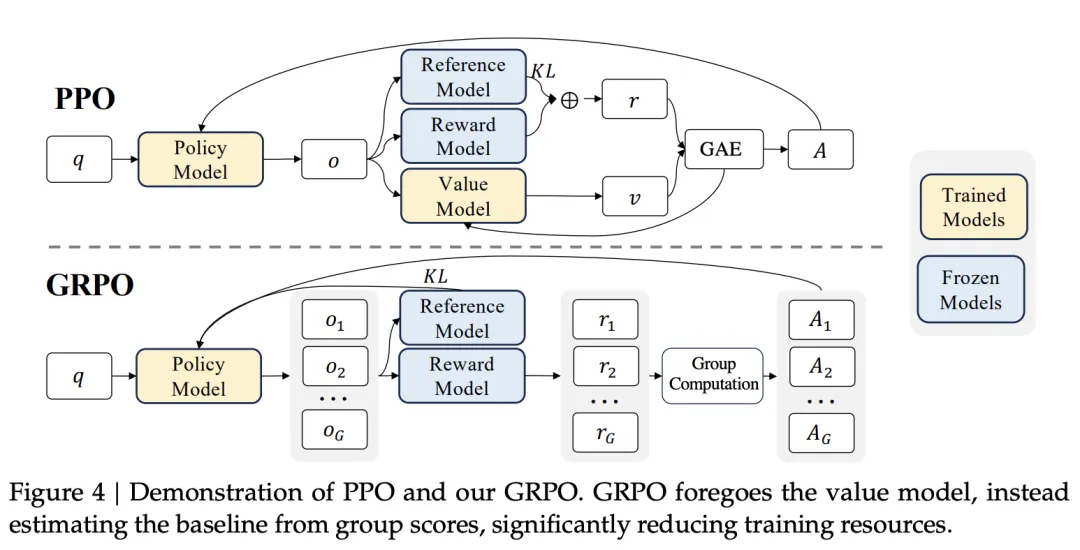
\includegraphics{images/image-0020.png}
\caption{PPO与GRPO架构对比}
\end{figure}

图中可以看出，PPO需要额外训练Value Model来估计价值基准，而GRPO冻结参考模型并使用组内样本奖励来估计Baseline，因此可以省去Critic网络。

\hypertarget{ux7fa4ux4f53ux91c7ux6837ux4ee3ux66ffux671fux671bux8ba1ux7b97}{%
\subsubsection{1. 群体采样（代替期望计算）}\label{ux7fa4ux4f53ux91c7ux6837ux4ee3ux66ffux671fux671bux8ba1ux7b97}}

对于每一个输入 \(q\)，我们使用旧策略 \(\pi_{\theta_{\mathrm{old}}}\) 采样一组共 \(G\) 个输出：

\[
\{o_1,o_2,\ldots,o_G\}\sim \pi_{\theta_{\mathrm{old}}}(O\mid q)
\]

随后，我们对每个输出计算奖励 \(\{r_1,r_2,\ldots,r_G\}\)。

\hypertarget{ux4f18ux52bfux4f30ux8ba1}{%
\subsubsection{2. 优势估计}\label{ux4f18ux52bfux4f30ux8ba1}}

这是GRPO取代Critic网络的关键。传统的A2C/PPO使用神经网络 \(V_{\phi}(s)\) 预测基准值，而在GRPO中，我们利用当前这组样本的平均奖励作为基准。

计算第 \(i\) 个样本的优势 \(A_i\)：

\[
A_i=\frac{r_i-\mu_{\mathrm{group}}}{\sigma_{\mathrm{group}}+\epsilon}
\]

其中 \(\mu_{\mathrm{group}}\) 表示当前组奖励均值，\(\sigma_{\mathrm{group}}\) 表示当前组奖励标准差。

除以标准差是因为考虑到不同类型的问题给分模式不同，可能互相不可比，故将其标准化。但也可能带来问题，比如对于过于难或简单的问题，几乎所有回答得分都一样时，该问题权重会被人为拉大。针对此问题后续已有工程上的优化。

\hypertarget{ux76eeux6807ux51fdux6570ux4e0eux957fux5ea6ux5f52ux4e00ux5316}{%
\subsubsection{3. 目标函数与长度归一化}\label{ux76eeux6807ux51fdux6570ux4e0eux957fux5ea6ux5f52ux4e00ux5316}}

目标函数 \(J(\theta)\) 如下：

\[
\mathcal{J}_{\mathrm{GRPO}}(\theta)=
\mathbb{E}_{q\sim P(Q),\{o_i\}_{i=1}^{G}\sim\pi_{\theta_{\mathrm{old}}}(O\mid q)}
\left[
\frac{1}{G}\sum_{i=1}^{G}\frac{1}{T_i}\sum_{t=1}^{T_i}
\left(
\min(\rho_{i,t}A_i,\mathrm{clip}(\rho_{i,t},1-\epsilon,1+\epsilon)A_i)-\beta D_{\mathrm{KL},t}
\right)
\right]
\]

这里Clip和KL同时存在，二者作用略有不同。Clip限制单次梯度更新的幅度，防止策略在一次迭代中变化过大导致训练崩塌；KL项保证最终策略距离初始参考策略不太远，关注累积效应，保证模型不会为了取得更高Reward而让语言能力退化。

这里 \(\rho_{i,t}\) 表示当前策略相对旧策略的概率比，\(D_{\mathrm{KL},t}\) 表示当前Token位置的KL惩罚项。对旧策略采样分布求期望后，可以得到策略和参考模型之间的KL约束；这里不需要遍历词表中的所有词，因为遍历通常是为了求期望，而组采样蒙特卡洛已经能近似得到该期望。

之所以用反向KL散度而非前向KL散度，是因为反向KL散度 \(KL(\pi_{\theta}\Vert\pi_{\mathrm{ref}})\) 会对当前策略高概率、参考策略低概率的区域给出较大惩罚，进而呈现``模式搜索''行为，让新的概率空间收敛到预训练后概率较大的空间里的特定模式（如果跳出空间往往表现为输出乱码、不符合正常语义的内容等，即``模式崩塌''）；前向KL散度则会倾向于覆盖预训练后的高概率空间，呈现``均值搜索''行为。RL获得的空间往往是预训练的子集（这也可能是RL难以让模型获得预训练完全没见过的技能的原因之一）。

方括号内，对于同一个输入，从第1到第 \(G\) 个输出取平均，然后是一个长度归一化项。这个长度归一化项是GRPO的另一个关键。

标准的策略梯度下，我们优化的目标是总奖励的期望：

\[
J=\mathbb{E}_{\tau\sim\pi_{\theta}}[R(\tau)]
\]

其梯度是（忽略Baseline）：

\[
\nabla J\approx \sum_{t=1}^{T}\nabla\log\pi_{\theta}(a_t\mid s_t)\cdot R
\]

目标函数 \(J\) 的梯度是对每一个动作的策略计算并累加的。假设 \(J\) 对每个动作的梯度大小为1，那么长为100的序列得到的梯度就约为长为10的序列的十倍，这会导致模型被长序列主导更新。但对于同一个问题而言，每个答案序列贡献的梯度应该是``平等''的，故我们需要除以序列长度 \(T\)：

\[
\nabla J_{\mathrm{GRPO}}\approx \frac{1}{T}\sum_{t=1}^{T}\nabla\log\pi_{\theta}(a_t\mid s_t)\cdot A
\]

但这也会产生一个问题，那就是当我们把 \(J\) 的梯度除以 \(T\) 时，意味着把目标函数 \(J\) 本身也除以了 \(T\)，目标函数变成了``单位Token能获得的奖励的期望''。这会导致模型在回答错误时生成大量无用的Token。原因在于：

当优势函数为正值时，意味着生成的结果是正确的，目标函数为正。由于目标函数是``单位Token能获得的奖励的期望''（有分母 \(T\)），为了让目标函数变大，策略在优化过程中会倾向于生成简短的正确答案，即这样的答案会产生比其他答案更大的梯度更新幅度。

当优势函数为负值时，意味着生成的结果是错误的，目标函数为负。为了让目标函数变大（惩罚的绝对值变小），策略会倾向于生成较长的答案（因为目标函数中除以较大 \(T\)），即这样的答案受到的负向惩罚和梯度压力反而更小。

\hypertarget{ux4e09ux4f18ux52bfux51fdux6570ux4f30ux8ba1ux7684ux6709ux504fux6027ux95eeux9898ux53caux89e3ux51b3ux65b9ux6848}{%
\subsection{三、优势函数估计的有偏性问题及解决方案}\label{ux4e09ux4f18ux52bfux51fdux6570ux4f30ux8ba1ux7684ux6709ux504fux6027ux95eeux9898ux53caux89e3ux51b3ux65b9ux6848}}

GRPO的优势函数估计看似是无偏的，实则往往对难题低估、对简单题高估。例如，一次取8条路径，对于一道答对概率只有1\%的难题，答对奖励为1，答错奖励为0，则8条路径都答错时没有梯度；有一条答对时，答对的那条路径优势函数为 \(1-\frac{1}{8}=\frac{7}{8}\)，但实际上优势函数为 \(1-\frac{1}{100}=\frac{99}{100}\)。对于简单题则相反，如答对概率为99\%，一条答错，答对者优势函数即为 \(\frac{1}{8}\)，实际上只有 \(\frac{1}{100}\)。

对此，可将难题优势函数乘以更大系数，简单题优势函数乘以更小系数，以尽可能实现无偏估计。

\hypertarget{ux53c2ux8003ux6587ux732e-83}{%
\subsection{参考文献}\label{ux53c2ux8003ux6587ux732e-83}}

\begin{itemize}
\tightlist
\item
  Shao, Z., Wang, P., Zhu, Q., et al.~(2024). \href{https://arxiv.org/abs/2402.03300}{DeepSeekMath: Pushing the Limits of Mathematical Reasoning in Open Language Models}. arXiv:2402.03300.
\end{itemize}

\clearpage

\hypertarget{klux6563ux5ea6ux7684ux9009ux62e9}{%
\section{KL散度的选择}\label{klux6563ux5ea6ux7684ux9009ux62e9}}

\hypertarget{ux4e00llmux4e2dux7684klux6563ux5ea6}{%
\subsection{一、LLM中的KL散度}\label{ux4e00llmux4e2dux7684klux6563ux5ea6}}

在大模型中，KL散度衡量输出概率分布的差异，并非按输出前的隐藏层维度计算，而是在大小为 \(V\) 的词表上计算（因为本质上大模型的输出是离散的tokens）。

\(D(P \Vert Q)=\sum_{i=1}^{V}p_i\log\frac{p_i}{q_i}\)，相当于 \(\log(p_i/q_i)\) 在 \(p\) 分布上的期望。

对于LLM，自回归输出 \(n\) 个token的KL散度：

\[
D_{KL}(P(Y) \Vert Q(Y))=\sum_Y P(Y)\log\frac{P(Y)}{Q(Y)}
\]

由于直接对所有可能的序列求和是不可行的（有 \(V^n\) 种可能），需利用自回归特性分解：

\[
\begin{aligned}
D_{KL}(P(Y) \Vert Q(Y))
&= \mathbb{E}_{Y\sim P}\left[\sum_{t=1}^{n}\left(\log P(y_t\mid y_{<t})-\log Q(y_t\mid y_{<t})\right)\right] \\
&= \sum_{t=1}^{n}\mathbb{E}_{Y\sim P}\left[\log\frac{P(y_t\mid y_{<t})}{Q(y_t\mid y_{<t})}\right]
\end{aligned}
\]

这里的处理难点在于 \(Y\sim P\)，需要考虑整个序列的概率分布。注意到右边的条件概率的条件为 \(y_{<t}\)，对于给定已知的 \(y_{<t}\) 分布，由自回归特性，\(y_t\) 的分布也会随之确定，\(Y=\{y_1,\ldots,y_t\}\) 的分布也就已知。因此可以改写为：

\[
D_{KL}(P(Y) \Vert Q(Y))
=\sum_{t=1}^{n}\mathbb{E}_{y_{<t}\sim P(y_{<t})}\left[
D_{KL}\left(P(y_t\mid y_{<t}) \Vert Q(y_t\mid y_{<t})\right)
\right]
\]

这意味着，两个序列分布的KL散度，等于每一步条件概率分布之间KL散度的期望之和（期望是基于分布P生成的历史轨迹计算的）。利用蒙特卡洛估计，在策略P下生成的各轨迹平均即可近似策略P下的期望。

\hypertarget{ux4e8ck1ux4f30ux8ba1ux5668ux548ck3ux4f30ux8ba1ux5668}{%
\subsection{二、K1估计器和K3估计器}\label{ux4e8ck1ux4f30ux8ba1ux5668ux548ck3ux4f30ux8ba1ux5668}}

对于长度为T的序列：

\textbf{K1 估计器（The Naïve Estimator）}

这是最直观的蒙特卡洛估计，直接计算 log 似然比：

\[
K1=\sum_{t=1}^{T}K1_t
=\sum_{t=1}^{T}\log\frac{\pi_\theta(y_t\mid x,y_{<t})}{\pi_{\mathrm{ref}}(y_t\mid x,y_{<t})}
\]

特点：它是 \(D_{KL}(\pi_\theta \Vert \pi_{\mathrm{ref}})\) 的无偏估计，但在实践中方差较大。

\textbf{K3 估计器（The Schulman Estimator）}

由 John Schulman 提出，旨在减少方差。它利用了 \(\log(x)\le x-1\) 的性质来逼近：

\[
K3=\sum_{t=1}^{T}K3_t
=\sum_{t=1}^{T}\left(
\frac{\pi_{\mathrm{ref}}(y_t\mid x,y_{<t})}{\pi_\theta(y_t\mid x,y_{<t})}
-1
-\log\frac{\pi_{\mathrm{ref}}(y_t\mid x,y_{<t})}{\pi_\theta(y_t\mid x,y_{<t})}
\right)
\]

特点：它也是 \(D_{KL}(\pi_\theta \Vert \pi_{\mathrm{ref}})\) 的无偏估计（期望为 KL 散度值），且具有比 K1 更低的方差。

KL散度项可以减在Reward或加在Loss里。在实际训练中，K1 in loss和K3 in reward不稳定，一般采用K3 in loss（方差更小）或K1 in reward（梯度无偏）。GRPO默认前者，但2025年有研究证明后者实际上可能性能更优，因为前者本身无偏但其梯度有偏。

\hypertarget{ux4e09ux8bc1ux660ek1-in-rewardux68afux5ea6ux65e0ux504fux53cak3-in-lossux68afux5ea6ux6709ux504f}{%
\subsubsection{（三）证明K1 in reward梯度无偏及K3 in loss梯度有偏}\label{ux4e09ux8bc1ux660ek1-in-rewardux68afux5ea6ux65e0ux504fux53cak3-in-lossux68afux5ea6ux6709ux504f}}

我们需要优化的真实目标（Reverse KL）的梯度为：

\[
\nabla_\theta D_{KL}(\pi_\theta \Vert \pi_{\mathrm{ref}})
=\mathbb{E}_{y\sim\pi_\theta}\left[
\log\frac{\pi_\theta}{\pi_{\mathrm{ref}}}\nabla_\theta\log\pi_\theta
\right]
\]

注：为简化符号，省略条件 \(x\) 和求和符号，关注核心各项。

\textbf{推导 1：K1 in Reward（无偏）}

当把 K1 放入 Reward 时，我们不对 K1 本身求导（视为常数奖励），而是利用 REINFORCE/PPO 的性质：

\[
\mathrm{Gradient}
=\mathbb{E}_{y\sim\pi_\theta}\left[K1\cdot\nabla_\theta\log\pi_\theta\right]
\]

代入 \(K1=\log\frac{\pi_\theta}{\pi_{\mathrm{ref}}}\)：

\[
\mathrm{Gradient}
=\mathbb{E}_{y\sim\pi_\theta}\left[
\left(\log\frac{\pi_\theta}{\pi_{\mathrm{ref}}}\right)
\nabla_\theta\log\pi_\theta
\right]
\]

结论：这与 Reverse KL 的真实梯度表达式完全一致，因此是无偏的。

\textbf{推导 2：K3 in Loss（有偏）}

当把 K3 放入 Loss 时，我们直接计算 \(\nabla_\theta K3\) 的期望。设比率 \(r=\frac{\pi_{\mathrm{ref}}}{\pi_\theta}\)，则 \(K3=r-1-\log r\)。注意 \(\log r=\log\pi_{\mathrm{ref}}-\log\pi_\theta\)。

我们需要计算 \(\mathbb{E}_{y\sim\pi_\theta}[\nabla_\theta K3]\)。首先看 \(\nabla_\theta K3\) 的各项：

\begin{enumerate}
\def\labelenumi{\arabic{enumi}.}
\tightlist
\item
  \(\nabla_\theta r=\nabla_\theta(\pi_{\mathrm{ref}}\cdot\pi_\theta^{-1})=\pi_{\mathrm{ref}}\cdot(-1)\pi_\theta^{-2}\cdot\nabla_\theta\pi_\theta=-\frac{\pi_{\mathrm{ref}}}{\pi_\theta}\cdot\frac{\nabla_\theta\pi_\theta}{\pi_\theta}=-r\nabla_\theta\log\pi_\theta\)
\item
  \(\nabla_\theta(-1)=0\)
\item
  \(\nabla_\theta(-\log r)=\nabla_\theta(\log\pi_\theta-\log\pi_{\mathrm{ref}})=\nabla_\theta\log\pi_\theta\)（假设 \(\pi_{\mathrm{ref}}\) 固定）
\end{enumerate}

合并各项得到 \(\nabla_\theta K3\)：

\[
\nabla_\theta K3
=-r\nabla_\theta\log\pi_\theta+\nabla_\theta\log\pi_\theta
=(1-r)\nabla_\theta\log\pi_\theta
\]

现在计算其期望：

\[
\mathbb{E}_{y\sim\pi_\theta}[\nabla_\theta K3]
=\mathbb{E}_{y\sim\pi_\theta}\left[(1-r)\nabla_\theta\log\pi_\theta\right]
\]

\[
\begin{aligned}
&=\mathbb{E}_{y\sim\pi_\theta}\left[\nabla_\theta\log\pi_\theta\right]
-\mathbb{E}_{y\sim\pi_\theta}\left[
\frac{\pi_{\mathrm{ref}}}{\pi_\theta}\nabla_\theta\log\pi_\theta
\right] \\
&=-\mathbb{E}_{y\sim\pi_\theta}\left[
\frac{\pi_{\mathrm{ref}}}{\pi_\theta}\nabla_\theta\log\pi_\theta
\right]
\end{aligned}
\]

其中第一项为 \(0\)（Score Function property）。

对比真实梯度：

\begin{itemize}
\tightlist
\item
  真实 Reverse KL 梯度：\(\mathbb{E}\left[\log\left(\frac{\pi_\theta}{\pi_{\mathrm{ref}}}\right)\nabla\log\pi_\theta\right]\)
\item
  K3 in Loss 梯度：\(\mathbb{E}\left[-\frac{\pi_{\mathrm{ref}}}{\pi_\theta}\nabla\log\pi_\theta\right]\)
\end{itemize}

事实上，K3估计器梯度变成了对应前向KL散度的梯度，而非反向KL散度，导致模型训练中更倾向于覆盖已有模式，而非在模式内部探索奖励最高区域。

其中Score Function property：

\textbf{1. 数学推导（The ``Why''）}

我们要证明的是：

\[
\mathbb{E}_{y\sim\pi_\theta}\left[\nabla_\theta\log\pi_\theta(y)\right]=0
\]

证明步骤如下：

\textbf{第一步：展开期望的定义}。期望 \(\mathbb{E}\) 就是对所有可能的 \(y\) 进行加权求和（对于离散的 LLM token 序列是求和，连续空间是积分）。

\[
\mathbb{E}_{y\sim\pi_\theta}\left[\nabla_\theta\log\pi_\theta(y)\right]
=\sum_y \pi_\theta(y)\cdot\nabla_\theta\log\pi_\theta(y)
\]

\textbf{第二步：应用对数求导法则（Log-Derivative Trick）}。根据微积分中的链式法则，\(\nabla\log f(x)=\frac{\nabla f(x)}{f(x)}\)。将其应用到 \(\log\pi_\theta(y)\) 上：

\[
\nabla_\theta\log\pi_\theta(y)
=\frac{\nabla_\theta\pi_\theta(y)}{\pi_\theta(y)}
\]

\textbf{第三步：代回并约分}。将第二步的结果代回第一步的式子中：

\[
\sum_y \pi_\theta(y)\cdot
\frac{\nabla_\theta\pi_\theta(y)}{\pi_\theta(y)}
=\sum_y \nabla_\theta\pi_\theta(y)
\]

\textbf{第四步：交换求和与求导的顺序}。在满足一定正则性条件下，我们可以交换求和符号 \(\sum\) 和梯度符号 \(\nabla_\theta\)：

\[
\sum_y \nabla_\theta\pi_\theta(y)
=\nabla_\theta\left(\sum_y \pi_\theta(y)\right)
\]

\textbf{第五步：利用概率归一化性质}。这是最关键的一步。对于任何概率分布，其所有可能事件的概率之和必须恒等于 1：

\[
\sum_y \pi_\theta(y)=1
\]

因此：

\[
\nabla_\theta\left(\sum_y \pi_\theta(y)\right)
=\nabla_\theta(1)=0
\]

所以：

\[
\mathbb{E}_{y\sim\pi_\theta}\left[\nabla_\theta\log\pi_\theta(y)\right]=0
\]

\textbf{2. 直观理解（The Intuition）}

``概率质量守恒''梯度 \(\nabla_\theta\pi_\theta(y)\) 代表当我们微调参数 \(\theta\) 时，样本 \(y\) 出现的概率是增加还是减少。

\begin{itemize}
\tightlist
\item
  如果我们让某些样本的概率增加了（梯度为正），那么为了保持总概率之和永远为 1，必然有另一些样本的概率要减少（梯度为负）。
\item
  这个式子 \(\mathbb{E}[\nabla\log\pi]=\sum\nabla\pi\) 实际上就是在计算所有可能样本的概率变化量的总和。
\item
  因为总概率（这个``蛋糕''的大小）是固定的 1，所以所有变化的加和必须为 0。
\end{itemize}

\hypertarget{ux53c2ux8003ux6587ux732e-84}{%
\subsection{参考文献}\label{ux53c2ux8003ux6587ux732e-84}}

\begin{itemize}
\tightlist
\item
  Schulman, J. (2020). \href{http://joschu.net/blog/kl-approx.html}{Approximating KL Divergence}.
\item
  Ziegler, D. M., Stiennon, N., Wu, J., et al.~(2019). \href{https://arxiv.org/abs/1909.08593}{Fine-Tuning Language Models from Human Preferences}. arXiv:1909.08593.
\item
  Ouyang, L., Wu, J., Jiang, X., et al.~(2022). \href{https://arxiv.org/abs/2203.02155}{Training language models to follow instructions with human feedback}. NeurIPS 2022.
\item
  Ahmadian, A., Cremer, C., Gallé, M., et al.~(2024). \href{https://arxiv.org/abs/2402.14740}{Back to Basics: Revisiting REINFORCE Style Optimization for Learning from Human Feedback in LLMs}. ACL 2024.
\end{itemize}

\clearpage

\hypertarget{ux4e3aux4ec0ux4e48online-rlux6bd4sftux66f4ux80fdux907fux514dux707eux96beux6027ux9057ux5fd8}{%
\section{为什么Online RL比SFT更能避免``灾难性遗忘''}\label{ux4e3aux4ec0ux4e48online-rlux6bd4sftux66f4ux80fdux907fux514dux707eux96beux6027ux9057ux5fd8}}

研究指出，On-Policy RL在避免``灾难性遗忘''上优于SFT（《RL'S RAZOR: WHY ONLINE REINFORCEMENT LEARNING FORGETS LESS》，MIT，2025）。相比于利用SFT微调，用On-Policy RL微调后的模型输出的策略与原预训练模型输出策略间的KL散度更小。（这里的KL散度工程上用的是在输入为新任务的情况下求出的期望，这是一个经验性的发现，即模型在新任务上的分布偏移量能预测它在旧任务上的遗忘程度；论文预测指标是Forward KL，但也指出RL之所以遗忘少，是因为它在优化过程中隐式地最小化了反向KL散度）

\hypertarget{ux4e00ux6838ux5fc3ux539fux56e0}{%
\subsection{一、核心原因}\label{ux4e00ux6838ux5fc3ux539fux56e0}}

SFT（Offline）：使用外部固定的数据集。这些数据的分布可能与模型当前的分布相去甚远。SFT 会强制将模型输出拉向这个任意的外部分布。由于解空间很大，外部数据往往会将模型引导至一个距离当前位置很远的最优解，导致剧烈的KL偏移，进而引发遗忘。论文发现，使用Off-Policy RL也存在类似问题。

RL（On-Policy）：使用模型自身生成的样本。On-Policy RL的更新逻辑是：对模型自己按当前策略生成的样本进行重加权，增加高奖励样本的概率，降低低奖励样本的概率。因为样本来自自身策略 \(\pi\)，RL的更新本质上是在当前分布的邻域内进行调整。它不会像SFT那样被强行拉向一个未知的、可能正交于原知识表示的分布。相反，On-Policy RL倾向于在满足新任务要求的前提下，寻找一条KL变化最小的路径。

\hypertarget{ux4e8cux4eceux6295ux5f71ux7684ux89c6ux89d2ux770brlux7684ux6536ux655b}{%
\subsection{二、从投影的视角看RL的收敛}\label{ux4e8cux4eceux6295ux5f71ux7684ux89c6ux89d2ux770brlux7684ux6536ux655b}}

标准的策略梯度方法本质上就是一个在``可行策略空间''和``最优解空间''之间，交替进行两种投影的算法：

假设我们处于一个简化的二值奖励（Binary Reward，\(R \in \{0,1\}\)）场景中：

\textbf{第一步：E-Step（I-Projection / 信息投影）}。这一步并不是在更新神经网络参数，而是在\textbf{构建目标分布}。当我们用当前策略 \(\pi_t\) 采样，并根据奖励 \(R\) 进行筛选（例如只保留 \(R=1\) 的样本，即 Rejection Sampling）时，我们实际上构建了一个新的非参数化分布 \(q_t\)。

论文证明（Lemma A.1），这个重加权后的分布 \(q_t\)，在数学上是所有满足``最优性条件''（即 \(\mathbb{E}_q[R]=1\)）的分布中，距离当前策略 \(\pi_t\) KL 散度最近的那一个：

\[
q_t = \arg\min_{q:\mathbb{E}_q[R]=1} D_{KL}(q\Vert \pi_t)
\]

直观理解：这相当于在``高分答案集合''中找一个离我现在怎么说话最像的分布。

\textbf{第二步：M-Step（M-Projection / 矩投影）}。这一步才是我们熟悉的梯度下降更新参数。当我们计算策略梯度 \(\nabla \mathbb{E}[R]\) 并更新 \(\pi\) 时，论文证明（Lemma A.2）这等价于让新的参数化策略 \(\pi_{t+1}\) 去拟合上述的理想分布 \(q_t\)。

这实际上是在最小化 \(D_{KL}(q_t\Vert \pi)\)（即交叉熵损失）：

\[
\pi_{t+1} = \arg\min_{\pi\in\Pi} D_{KL}(q_t\Vert \pi)
\]

直观理解：修改我的模型参数，让它尽可能模仿刚才那个``既得了高分又离我很近''的理想分布 \(q_t\)。

从而这种连续的投影过程最终收敛到的解，理论上是所有能完成任务（最优）的策略中，距离初始策略的KL散度最小的那一个。

\begin{figure}[htbp]
\centering
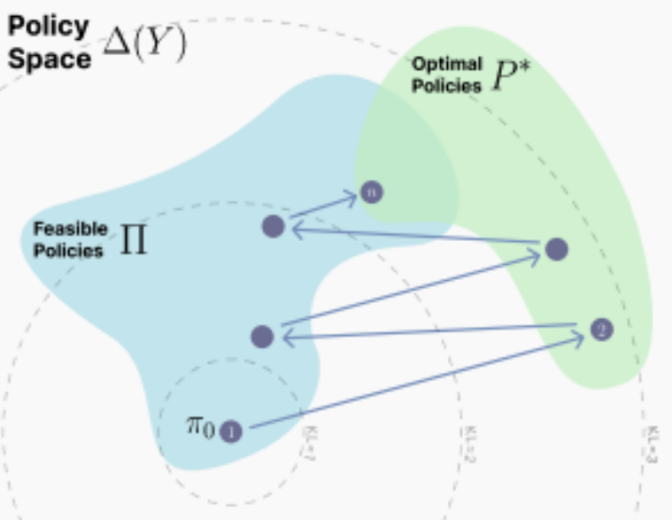
\includegraphics{images/image-0021.png}
\caption{Policy Space / Feasible Policies / Optimal Policies 概念图}
\end{figure}

下面证明这两步过程和On-Policy RL的等价性：

\hypertarget{ux7b2cux4e00ux6b65ux4e3aux4ec0ux4e48ux62d2ux7eddux91c7ux6837ux7b49ux4ef7ux4e8e-i-projection}{%
\subsubsection{第一步：为什么``拒绝采样''等价于 I-Projection？}\label{ux7b2cux4e00ux6b65ux4e3aux4ec0ux4e48ux62d2ux7eddux91c7ux6837ux7b49ux4ef7ux4e8e-i-projection}}

\textbf{结论：}从当前策略 \(p\) 中进行拒绝采样（Rejection Sampling），得到的分布 \(q_{RS}\)，正是满足``奖励约束''且距离 \(p\) KL 散度最小的分布。

\textbf{证明过程：}

\textbf{1. 定义场景：}

\begin{itemize}
\tightlist
\item
  \(p(y)\) 是当前策略（Base distribution）。
\item
  \(R(y) \in \{0,1\}\) 是二值奖励函数。
\item
  \(S=\{y\in Y:R(y)=1\}\) 是所有正确答案的集合（即获得奖励的样本）。
\item
  拒绝采样的过程是：从 \(p\) 采样，保留 \(y\in S\)。这产生的经验分布实际上就是条件概率分布 \(p(y\mid S)\)。
\end{itemize}

\textbf{2. 构建优化目标（I-Projection）：}我们需要寻找一个分布 \(q\)，使得它在满足期望奖励为 1 的前提下，与 \(p\) 最接近：

\[
\min_q D_{KL}(q\Vert p) \quad \mathrm{s.t.}\quad \mathbb{E}_{y\sim q}[R(y)] = 1
\]

\textbf{3. 推导等价性：}

约束条件 \(\mathbb{E}_{y\sim q}[R(y)]=1\) 意味着分布 \(q\) 的所有概率质量必须全部落在集合 \(S\) 上；如果 \(q\) 在非 \(S\) 区域有值，期望奖励就会小于 1。因此，\(q\) 的支持集（Support）必须包含在 \(S\) 内。

对于任意支持集在 \(S\) 上的分布 \(q\)，我们可以将 \(p(y)\) 分解为 \(p(y)=p(S)p(y\mid S)\)。代入 KL 散度公式：

\[
D_{KL}(q\Vert p)
= \sum_{y\in S} q(y)\ln\frac{q(y)}{p(y)}
= \sum_{y\in S} q(y)\ln\frac{q(y)}{p(S)p(y\mid S)}
\]

拆解对数项：

\[
D_{KL}(q\Vert p)
= \sum_{y\in S} q(y)\ln\frac{q(y)}{p(y\mid S)}
- \sum_{y\in S} q(y)\ln p(S)
\]

因为 \(\sum_{y\in S}q(y)=1\)，且 \(p(S)\) 是常数，第二项与 \(q\) 无关。第一项正是 \(D_{KL}(q\Vert p(\cdot\mid S))\)。

由 KL 散度的性质（\(D_{KL}\ge 0\)，当且仅当两个分布相等时为 0），要最小化上式，必须有 \(q(y)=p(y\mid S)\)。

也就是说当我们将RL中概率分布的调整简化为拒绝采样的情形后，它在数学上就严格等价于找到了一个理论上的最优目标分布。

\hypertarget{ux7b2cux4e8cux6b65ux4e3aux4ec0ux4e48ux7b56ux7565ux68afux5ea6ux7b49ux4ef7ux4e8e-m-projection}{%
\subsubsection{第二步：为什么``策略梯度''等价于 M-Projection？}\label{ux7b2cux4e8cux6b65ux4e3aux4ec0ux4e48ux7b56ux7565ux68afux5ea6ux7b49ux4ef7ux4e8e-m-projection}}

\textbf{结论：}使用策略梯度（Policy Gradient）更新参数化策略 \(\pi\)，等价于让 \(\pi\) 去拟合（投影到）上一步生成的目标分布 \(q\)。

\textbf{证明过程：}

\textbf{1. 定义目标分布：}设上一步得到的理想分布为 \(q(y)\)。在 RL 中，这通常是根据奖励重加权后的分布：

\[
q(y)=\frac{\pi_{\mathrm{old}}(y)R(y)}{Z}
\]

其中 \(Z\) 是归一化常数。

\textbf{2. 构建优化目标（M-Projection）：}我们需要找到一个新的参数化策略 \(\pi\)，使其尽可能接近理想分布 \(q\)：

\[
\min_\pi D_{KL}(q\Vert \pi)
\]

\textbf{3. 推导等价性：}

展开 KL 散度公式：

\[
D_{KL}(q\Vert \pi)
= \sum_y q(y)\ln\frac{q(y)}{\pi(y)}
= \sum_y q(y)\ln q(y)-\sum_y q(y)\ln\pi(y)
\]

第一项 \(\sum_y q(y)\ln q(y)\) 是目标分布的熵相关项，对于优化变量 \(\pi\) 来说是常数。因此，最小化 KL 散度等价于最大化第二项：

\[
\max_\pi \mathbb{E}_{y\sim q}[\ln \pi(y)]
\]

将 \(q(y)\) 的定义代回：

\[
\max_\pi \sum_y \frac{\pi_{\mathrm{old}}(y)R(y)}{Z}\ln\pi(y)
\]

忽略常数 \(Z\)，这等价于最大化：

\[
\mathbb{E}_{y\sim \pi_{\mathrm{old}}}[R(y)\ln\pi(y)]
\]

这正是标准策略梯度的一步更新目标。把采样分布固定为 \(\pi_{\mathrm{old}}\) 时，对 \(\mathbb{E}_{y\sim\pi_{\mathrm{old}}}[R(y)\ln\pi(y)]\) 求梯度，就得到策略梯度定理中的 \(R(y)\nabla\ln\pi(y)\) 形式。

策略梯度的更新过程，本质上就是在一个参数化的分布族中，寻找一个 \(D_{KL}(q\Vert \pi)\) 最小的解，让神经网络输出策略分布 \(\pi\) 尽可能拟合实际最优策略分布 \(q\)（但神经网络输出不可能总是完全和实际分布相同，故取不到零）。

这两个步骤共同构成了一个 EM 算法（Expectation-Maximization）的变体：

E-Step（I-Projection）：用拒绝采样隐式地构造出最优目标分布 \(q\)（非参数化的）。

M-Step（M-Projection）：用策略梯度更新参数 \(\pi\)，使其逼近 \(q\)。

正是因为每一步 M-Projection 都是在拉近 \(\pi\) 和 \(q\)（而 \(q\) 又是 \(\pi\) 自身的重加权），所以整个轨迹被约束在一条 KL 变化最小的路径上，从而避免了 SFT 那种因拟合外部分布而导致的剧烈参数漂移和遗忘。

\hypertarget{ux53c2ux8003ux6587ux732e-85}{%
\subsection{参考文献}\label{ux53c2ux8003ux6587ux732e-85}}

\begin{itemize}
\tightlist
\item
  Shenfeld, I., Pari, J., \& Agrawal, P. (2025). \href{https://arxiv.org/abs/2509.04259}{RL's Razor: Why Online Reinforcement Learning Forgets Less}. arXiv:2509.04259.
\end{itemize}

\clearpage


% 模型压缩
\hypertarget{ux6a21ux578bux538bux7f29}{%
\chapter{模型压缩}\label{ux6a21ux578bux538bux7f29}}

\hypertarget{ux6a21ux578bux91cfux5316}{%
\section{模型量化}\label{ux6a21ux578bux91cfux5316}}

\hypertarget{ux4e00ux6a21ux578bux91cfux5316ux7684ux6838ux5fc3ux601dux60f3}{%
\subsection{一、模型量化的核心思想}\label{ux4e00ux6a21ux578bux91cfux5316ux7684ux6838ux5fc3ux601dux60f3}}

由于大模型的计算、存储开销巨大，计算需要的时间较长，在大模型推理部署时，我们考虑降低模型中数值的精度，以使模型无需在专业的GPU上就可以运行。一般我们会将模型的32位浮点数转换为8位整数（有时还会选择转换为4位整数）格式。

值得注意的是，由于模型训练过程需要精确的参数进行梯度更新，模型训练时不应量化。对于物理模拟等对数值精度要求高的领域，也不宜运用模型量化。

\hypertarget{ux4e8c8-bitux91cfux5316}{%
\subsection{二、8-bit量化}\label{ux4e8c8-bitux91cfux5316}}

8-bit量化即量化为{[}-128,127{]}范围内的整数，共有256个可能的取值。

\hypertarget{ux5bf9ux79f0ux91cfux5316}{%
\subsubsection{1. 对称量化}\label{ux5bf9ux79f0ux91cfux5316}}

在这个示例张量中，绝对值最大的数是 \(10.8\)。为了保持对称量化，浮点有效范围扩展为 \([-10.8, 10.8]\)，再映射到 INT8 的对称区间。

\begin{longtable}[]{@{}rr@{}}
\toprule
浮点值 \(x\) & 对应 INT8 值 \(q\) \\
\midrule
\endhead
\(-7.59\) & \(-89\) \\
\(-4.57\) & \(-54\) \\
\(-1.95\) & \(-23\) \\
\(0\) & \(0\) \\
\(3.08\) & \(36\) \\
\(5.47\) & \(64\) \\
\(10.8\) & \(127\) \\
\bottomrule
\end{longtable}

寻找绝对值最大值：为了保持对称，必须以数据中绝对值最大的数为边界，定义新的量化范围（Clip Range）。

\[
\alpha = \max(|-7.59|, |10.8|) = 10.8
\]

因此，量化的有效浮点范围被扩展为 \([-10.8, 10.8]\)。

计算缩放因子 \(S\)：将上述浮点范围映射到 INT8 的对称区间 \([-127, 127]\)。

\[
S = \frac{10.8}{127} \approx 0.085039
\]

应用量化公式：由于 \(Z = 0\)，公式非常简洁：

\[
q = \mathrm{round}\left(\frac{x}{S}\right)
\]

\hypertarget{ux975eux5bf9ux79f0ux91cfux5316}{%
\subsubsection{2. 非对称量化}\label{ux975eux5bf9ux79f0ux91cfux5316}}

非对称量化直接使用原始浮点范围 \([-7.59, 10.8]\)，其中最大值为 \(10.8\)，最小值为 \(-7.59\)。

\begin{longtable}[]{@{}rr@{}}
\toprule
浮点值 \(x\) & 对应 INT8 值 \(q\) \\
\midrule
\endhead
\(-7.59\) & \(-128\) \\
\(-4.57\) & \(-86\) \\
\(-1.95\) & \(-50\) \\
\(0\) & \(-23\) \\
\(3.08\) & \(20\) \\
\(5.47\) & \(53\) \\
\(10.8\) & \(127\) \\
\bottomrule
\end{longtable}

确定范围：

\begin{itemize}
\tightlist
\item
  浮点范围：\(x_{\min} = -7.59, x_{\max} = 10.8\)
\item
  整数范围（INT8）：\(q_{\min} = -128, q_{\max} = 127\)
\end{itemize}

计算缩放因子 \(S\)：

\[
S = \frac{x_{\max} - x_{\min}}{q_{\max} - q_{\min}}
  = \frac{10.8 - (-7.59)}{127 - (-128)}
  = \frac{18.39}{255}
  \approx 0.072117
\]

注：非对称量化的 \(S\)（\(0.072\)）小于对称量化的 \(S\)（\(0.085\)），说明其量化粒度更细，精度更高。

计算零点 \(Z\)：计算浮点数 \(0.0\) 对应的整数值 \(Z\)。

\[
Z = \mathrm{round}\left(q_{\max} - \frac{x_{\max}}{S}\right)
\]

代入数值：

\[
Z = \mathrm{round}\left(127 - \frac{10.8}{0.072117}\right)
  \approx \mathrm{round}(127 - 149.75)
  \approx -23
\]

这意味着浮点数 \(0.0\) 映射为整数 \(-23\)。

应用量化公式：

\[
q = \mathrm{round}\left(\frac{x}{S} + Z\right)
\]

计算示例：

\begin{itemize}
\tightlist
\item
  对于 \(10.8\)：
\end{itemize}

\[
q = \mathrm{round}\left(\frac{10.8}{0.072117} - 23\right)
  = \mathrm{round}(149.75 - 23)
  = 127
\]

\begin{itemize}
\tightlist
\item
  对于 \(-7.59\)：
\end{itemize}

\[
q = \mathrm{round}\left(\frac{-7.59}{0.072117} - 23\right)
  = \mathrm{round}(-105.24 - 23)
  = -128
\]

优点：如示意图所示，原始范围 \([-7.59, 10.8]\) 完整覆盖了 \([-128, 127]\)，没有浪费任何量化层级，通常能保留更高的精度。

缺点：计算稍复杂，反量化或矩阵运算时需要额外处理 \(Z\) 的减法运算。

\hypertarget{ux4e094-bitux91cfux5316}{%
\subsection{三、4-bit量化}\label{ux4e094-bitux91cfux5316}}

4-bit量化将每个权重表示为0000-1111，共有16个值。

核心思想：我们不应该让量化点的间隔相等，而应该让每个量化点所代表的``概率分位数''的概率间隔相等。我们将(0,1)正态分布的累积分布函数等分为16个概率区间，取各区间中点对应的值，归一化映射到{[}-1,1{]}范围，作为NF4量化值。这些值和量化索引一一对应，如-1.0000对应0000，-0.6962对应0001，\ldots\ldots，1.0000对应1111.

量化步骤：

\begin{enumerate}
\def\labelenumi{\arabic{enumi}.}
\item
  计算缩放因子 \(S\)，将权重张量的范围映射到 NF4 量化表的 \([-1, 1]\) 范围。

  \begin{itemize}
  \tightlist
  \item
    计算张量中每个元素的绝对值：\([0.45, 0.88, 1.54, 0.12, 0.05, 0.99, 0.33, 2.10]\)
  \item
    找到最大值：\(2.10\)
  \item
    因此，缩放因子 \(S = 2.10\)
  \end{itemize}
\item
  归一化权重，用每个原始权重除以缩放因子 \(S\)，得到归一化后的权重 \(R_{norm} = \frac{R}{S}\)。

  \begin{itemize}
  \tightlist
  \item
    \(0.45 / 2.10 = 0.214\)
  \item
    \(-0.88 / 2.10 = -0.419\)
  \item
    \ldots\ldots{}
  \item
    由此得到归一化后的张量 \(R_{norm}\)：\([0.214, -0.419, 0.733, -0.057, 0.024, 0.471, -0.157, -1.0]\)
  \end{itemize}
\item
  映射到距离最近的NF4量化点，转换为对应的4位NF4索引。
\item
  存储结果，经过量化，最终需要存储两样东西：

  \begin{itemize}
  \tightlist
  \item
    4比特索引数组：\([10, 3, 14, 6, 8, 12, 5, 0]\)
  \item
    缩放因子 \(S\)：\(2.10\)（用 FP32 存储）
  \end{itemize}
\end{enumerate}

这个块的原始内存占用是 \(8 \times 32\) 位 \(= 256\) 位，现在是 \(8 \times 4\) 位 \(+ 32\) 位 \(= 64\) 位，内存压缩了 75\%。

反量化步骤（转换回FP32）：

\begin{enumerate}
\def\labelenumi{\arabic{enumi}.}
\item
  读取索引和缩放因子。

  \begin{itemize}
  \tightlist
  \item
    从内存中读取之前存储的索引数组和缩放因子 \(S = 2.10\)。
  \end{itemize}
\item
  从量化表恢复归一化值：使用索引法，在 NF4 量化表中查找对应的浮点值。

  \begin{itemize}
  \tightlist
  \item
    \(10 \to 0.1906\)
  \item
    \(3 \to -0.3949\)
  \item
    \ldots{}
  \item
    由此得到恢复的归一化张量 \(R'_{norm}\)：\([0.1906, -0.3949, 0.6717, -0.0911, 0.0062, 0.4045, -0.1848, -1.0]\)
  \end{itemize}
\item
  乘以缩放因子恢复权重：将恢复的归一化值乘以缩放因子 \(S\)，得到最终的反量化权重 \(R'\)。

  \begin{itemize}
  \tightlist
  \item
    \(R' = R'_{norm}S\)
  \item
    \(0.1906 \times 2.10 = 0.400\)
  \item
    \(-0.3949 \times 2.10 = -0.829\)
  \item
    \ldots{}
  \item
    最终得到 \(R'\)：\([0.400, -0.829, 1.411, -0.191, 0.013, 0.849, -0.388, -2.10]\)
  \end{itemize}
\end{enumerate}

\hypertarget{ux56dbux9759ux6001ux91cfux5316ux4e0eux52a8ux6001ux91cfux5316}{%
\subsection{四、静态量化与动态量化}\label{ux56dbux9759ux6001ux91cfux5316ux4e0eux52a8ux6001ux91cfux5316}}

\hypertarget{ux9759ux6001ux91cfux5316}{%
\subsubsection{1. 静态量化}\label{ux9759ux6001ux91cfux5316}}

（1）核心思想和步骤

静态量化是一种``全流程量化''策略。它的核心在于``离线（Offline）''完成所有繁重的工作。

校准：这是静态量化最关键的一步。因为还没有运行模型，我们不知道激活值（Activation，即每一层的输出）的范围。所以需要喂入少量真实的典型数据（校准集），让模型跑一遍，统计每一层激活值的min和max，从而提前计算出固定的S和Z。

转换：一旦有了S和Z，就将模型中所有的权重和激活值的处理逻辑全部写成INT8格式。

推理：运行时，模型不再需要做任何浮点运算转换，直接在整数域飞快奔跑。（两个整数相加可能超出INT8，此时会用INT32计算后转回INT8）

（2）优缺点和用途

优点：推理速度最快。

缺点：如果真实数据分布相对于校准集发生变化（NLP任务中尤其多见），S和Z可能不再适用；对于涉及Softmax等变换的场景（如Transformer），量化带来的微小差异可能在指数运算被急剧放大；不擅长处理``离群值''（如注意力机制中，在设置S和Z时，权重分布往往呈现大部分集中和一些离群值的状态，离群值往往起着类似``注意力锚点''的关键作用，但如果照顾离群值，则大部分值精度急剧下降）。

用途：CNN、边缘设备等。

\hypertarget{ux52a8ux6001ux91cfux5316}{%
\subsubsection{2. 动态量化}\label{ux52a8ux6001ux91cfux5316}}

（1）核心思想和步骤

动态量化是一种``折中''策略，核心是``权重静态，激活动态''，准备阶段只把模型的权重提前量化成 INT8。推理时：

层间传输：上一层的输出是FP32，下一层的输入也是FP32。

计算前：在进入矩阵乘法（MatMul）核心计算之前，激活值是FP32。系统需要读取这些 FP32 数据，计算统计量，然后将其转换为INT8。

计算时：核心的矩阵乘法是用 INT8 完成的（得到 INT32 结果）。

计算后：乘以 Scale 因子，将结果反量化回FP32。

非线性层：LayerNorm、GELU/SiLU等激活函数层通常直接在FP32上运行，不进行量化。

（2）优缺点和应用

优点：虽然不如静态量化快，但对于LLM这种内存受限的模型，加载权重的时间远多于计算时间。动态量化将权重体积缩小了4倍，意味着从内存加载权重的速度快了4倍，是性能提升的主要来源，与静态量化间的时间差相比而言很小。

缺点：需要实时分析当前激活值的范围，每次推理都要做一次min()、max()和div() 运算，并且要逐元素将FP32转为INT8，增加CPU/GPU的负担；数据在INT8核心和FP32显存之间频繁转换，增加了指令延迟。

应用：对于 Transformer/LLM（参数巨大，计算相对稀疏），动态量化通常能带来1.5x到2x的推理加速。因为``加载权重的收益''远大于``动态计算量化参数的开销''；对于 CNN（如 ResNet，计算密集型），动态量化效果往往不如静态量化，甚至可能比纯FP32慢，因为 CNN 的权重复用率高，计算量大，频繁的动态转换开销占比过高。

\hypertarget{ux53c2ux8003ux6587ux732e-86}{%
\subsection{参考文献}\label{ux53c2ux8003ux6587ux732e-86}}

\begin{itemize}
\tightlist
\item
  Jacob, B., Kligys, S., Chen, B., et al.~(2018). \href{https://arxiv.org/abs/1712.05877}{Quantization and Training of Neural Networks for Efficient Integer-Arithmetic-Only Inference}. CVPR 2018.
\item
  Dettmers, T., Lewis, M., Belkada, Y., \& Zettlemoyer, L. (2022). \href{https://arxiv.org/abs/2208.07339}{LLM.int8(): 8-bit Matrix Multiplication for Transformers at Scale}. NeurIPS 2022.
\item
  Dettmers, T., Pagnoni, A., Holtzman, A., \& Zettlemoyer, L. (2023). \href{https://arxiv.org/abs/2305.14314}{QLoRA: Efficient Finetuning of Quantized LLMs}. NeurIPS 2023.
\end{itemize}

\clearpage

\hypertarget{ux6a21ux578bux84b8ux998f}{%
\section{模型蒸馏}\label{ux6a21ux578bux84b8ux998f}}

\hypertarget{ux4e00ux6838ux5fc3ux601dux60f3-7}{%
\subsection{一、核心思想}\label{ux4e00ux6838ux5fc3ux601dux60f3-7}}

在深度学习中，我们通常训练一个庞大、复杂的模型来获得高准确率。但在实际部署（如手机端、IoT 设备）时，由于算力和内存限制，无法直接使用这个大模型。我们让一个小模型（Student）通过模仿一个大模型（Teacher）的行为，来学习大模型中蕴含的``暗知识''，从而在保持较小参数规模的同时，尽可能达到接近大模型的性能。下面引入两个概念：

Hard Target（硬标签）：老师告诉学生：答案是``A''。这对应传统的交叉熵损失函数，即训练时专注增加输出 A 的概率，不关心输出 B、C 的概率。

Soft Target（软标签）：老师告诉学生：``答案选 A，但 B 也有点道理，C 是大错特错的。''这种包含概率分布的信息（如 A=0.7, B=0.2, C=0.1）蕴含了类别之间的相似度关系，即大模型内的``暗知识''。

模型蒸馏会同时学习这两种标签。（不可只学习软标签，那样会导致输出正确答案的概率下降）

\hypertarget{ux4e8cux6570ux5b66ux8868ux8fbe-2}{%
\subsection{二、数学表达}\label{ux4e8cux6570ux5b66ux8868ux8fbe-2}}

\hypertarget{ux5e26ux6e29ux5ea6ux7684-softmax}{%
\subsubsection{1. 带温度的 Softmax}\label{ux5e26ux6e29ux5ea6ux7684-softmax}}

在标准的分类任务中，神经网络输出 logits \(z_i\)，经过 Softmax 得到概率 \(q_i\)。在蒸馏中，我们引入超参数 \(T\)：

\[
q_i = \frac{\exp(z_i / T)}{\sum_j \exp(z_j / T)}
\]

\begin{itemize}
\tightlist
\item
  当 \(T = 1\) 时，这就是标准的 Softmax。
\item
  当 \(T > 1\) 时，概率分布变得更``平滑''（Softer）。这使得原本接近 0 的错误类别的概率被放大，从而暴露出模型学到的类别间的隐含关系（例如：在识别``狗''时，模型认为像``猫''的概率比像``汽车''的概率大）。
\end{itemize}

\hypertarget{ux635fux5931ux51fdux6570loss-function}{%
\subsubsection{2. 损失函数（Loss Function）}\label{ux635fux5931ux51fdux6570loss-function}}

学生模型的总损失函数 \(L\) 通常由两部分组成：

\[
L = \alpha L_{KD} + (1 - \alpha)L_{CE}
\]

其中：

\begin{itemize}
\tightlist
\item
  \(L_{KD}\)（蒸馏损失/软损失）：衡量学生模型产生的软概率分布与教师模型产生的软概率分布之间的差异。通常使用 KL 散度（Kullback-Leibler Divergence）。注意，计算此时使用的是高温 \(T\)。
\item
  \(L_{CE}\)（学生损失/硬损失）：衡量学生模型的输出与真实标签（Ground Truth）之间的差异。通常使用标准的交叉熵损失（Cross-Entropy Loss）。注意，计算此时使用的是 \(T = 1\)。
\item
  \(\alpha\)：平衡两个损失权重的超参数。
\end{itemize}

注意这里的 KL 散度是 forward KL，因为：

KL 散度的标准数学定义为：

\[
D_{KL}(P \Vert Q) = \mathbb{E}_{x \sim P}\left[\log \frac{P(x)}{Q(x)}\right]
\]

请注意公式中的期望符号 \(\mathbb{E}_{x \sim P}\)。这意味着我们要从分布 \(P\) 中采样数据来计算这个积分或求和。

在机器学习的语境下，谁负责在物理世界（或计算图中）生成采样数据，谁就必须排在 KL 散度的前面。

\hypertarget{ux6570ux5b66ux63a8ux5bfcux4e3aux4ec0ux4e48ux9ad8ux6e29ux6709ux6548}{%
\subsubsection{3. 数学推导：为什么高温有效？}\label{ux6570ux5b66ux63a8ux5bfcux4e3aux4ec0ux4e48ux9ad8ux6e29ux6709ux6548}}

假设 logits \(z_i\) 相比于 \(T\) 很小（即 \(z_i / T \ll 1\)），我们可以对 Softmax 函数进行泰勒展开。Softmax 输出 \(q_i\) 大约为：

\[
q_i \approx \frac{1 + z_i / T}{N + \sum_j z_j / T}
\]

假设 logits 均值为 0（即 \(\sum_j z_j = 0\)），则简化为：

\[
q_i \approx \frac{1 + z_i / T}{N}
\]

假设我们使用交叉熵损失函数（或 KL 散度）进行蒸馏，其针对学生模型 Logit \(z_i^{(Student)}\) 的梯度通常形式为：

\[
\frac{\partial L}{\partial z_i^{(Student)}} = \frac{1}{T}\left(q_i^{(Student)} - q_i^{(Teacher)}\right)
\]

注：这里的 \(1/T\) 来自于链式法则中对 \(z_i / T\) 求导产生的系数。

现在，我们将上面的高温概率近似代入 \(q_i\)：

\[
\begin{aligned}
\frac{\partial L}{\partial z_i^{(Student)}} &\approx \frac{1}{T}\left[\left(\frac{1 + z_i^{(Student)} / T}{N}\right) - \left(\frac{1 + z_i^{(Teacher)} / T}{N}\right)\right] \\
&= \frac{1}{NT^2}\left(z_i^{(Student)} - z_i^{(Teacher)}\right)
\end{aligned}
\]

忽略常数系数 \(\frac{1}{NT^2}\)，我们发现梯度正比于：

\[
\frac{\partial L}{\partial z_i} \propto z_i^{(Student)} - z_i^{(Teacher)}
\]

回顾均方误差（MSE）的梯度：如果我们直接定义损失函数为 Logits 之间的 MSE：

\[
L_{MSE} = \frac{1}{2}\left(z^{(Student)} - z^{(Teacher)}\right)^2
\]

其梯度正是：

\[
\frac{\partial L_{MSE}}{\partial z^{(Student)}} = z^{(Student)} - z^{(Teacher)}
\]

这就证明了：在高温极限下，最小化 KL 散度（或软交叉熵）等价于最小化 Logits 之间的均方误差。

当然，实际上我们一般取 \(T\) 为 2\textasciitilde20，平衡 Hard Target 的``关注最大值''和 MSE 的``平衡关注各方向分布''。从实际意义上来说：

在正常温度下，Softmax 会把最大的 Logit 变成接近 1 的概率，而把其他 Logits 压缩成接近 0。

Teacher Logits: \texttt{{[}10,\ 5,\ 2{]}} -\textgreater{} Softmax: \texttt{{[}0.99,\ 0.009,\ 0.001{]}}

Teacher Logits: \texttt{{[}10,\ 8,\ 8{]}} -\textgreater{} Softmax: \texttt{{[}0.8,\ 0.1,\ 0.1{]}}

如果只看概率，很多细微的差异（比如 5 和 2 的区别）被``压扁''了，学生模型很难学到。

而 Logits 直接反映了模型对各个类别的原始置信度。

Logits \texttt{{[}10,\ 5,\ 2{]}} 明确告诉学生：虽然类别 1 最强，但类别 2 比类别 3 强得多（强 3 个单位），这种信息，就是暗知识（Dark Knowledge）。

上面模型蒸馏的数学表达，事实上正是``匹配 Logits''思想的体现。它的结果是：

\begin{itemize}
\tightlist
\item
  方向对齐：蒸馏过程要求学生生成的 Logits 向量 \(z_s\) 和教师的 Logits 向量 \(z_t\) 指向同一个方向。这意味着学生不仅要学会``谁是第一名''，还要学会``第二名、第三名\ldots\ldots 第 N 名''的相对排序。
\item
  相对大小对齐：\(z_i - z_j\) 代表了类别 \(i\) 和类别 \(j\) 的相对差距（Log-odds）。Logits Matching 强迫学生模型复刻这种相对差距。
\end{itemize}

例如，如果老师认为``猫''比``汽车''更像``狗''10 倍，学生也必须认为``猫''比``汽车''更像``狗''10 倍。

\hypertarget{ux4e09ux6a21ux578bux84b8ux998fux7684ux591aux79cdux65b9ux6cd5}{%
\subsection{三、模型蒸馏的多种方法}\label{ux4e09ux6a21ux578bux84b8ux998fux7684ux591aux79cdux65b9ux6cd5}}

\begin{enumerate}
\def\labelenumi{\arabic{enumi}.}
\item
  基于响应：利用教师模型最后一层的输出，这是最经典的方法（如上文所述）。
\item
  基于特征：不仅学习输出，还强制学生模型的中间层特征图拟合教师模型的中间层。通常需要引入额外的卷积层来匹配特征图的维度。
\end{enumerate}

损失函数：

\[
L_{\mathrm{Feature}} = \left\Vert F_{\mathrm{Teacher}}(x) - W_{\mathrm{reg}}\left(F_{\mathrm{Student}}(x)\right) \right\Vert^2
\]

\begin{enumerate}
\def\labelenumi{\arabic{enumi}.}
\setcounter{enumi}{2}
\tightlist
\item
  基于样本关系：
\end{enumerate}

对于同一批 \(N\) 个样本，分别获取它们在教师模型的特征空间中的特征向量（一般为其中一层的向量），以及在学生模型的特征空间中的特征向量。由于教师模型和学生模型特征向量维度不同，无法直接计算损失，故我们考虑计算向量两两之间的``相似度''（标量）。

我们对教师模型的这些特征向量两两计算余弦相似度或欧氏距离，得到 \(N \times N\) 的``相似度矩阵''，对学生模型也得到这样的矩阵。如果用的是欧氏距离，为了消除维度差异，我们还会加归一化因子。我们的目标是让这两个矩阵长得像，即结构一致性：

\[
L_{\mathrm{Relation}} = \sum_{i=1}^{N} \sum_{j=1}^{N} L_\delta\left(\mathcal{R}_{ij}^{(T)}, \mathcal{R}_{ij}^{(S)}\right)
\]

其中 \(L_\delta\) 可以是 Huber Loss 或 \(L_2\) Loss。

Huber Loss 是一种鲁棒回归损失函数，它结合了均方误差（MSE/L2）和平均绝对误差（MAE/L1）的优点。

简单来说，它的设计哲学是：``小错误用平方惩罚（为了平滑收敛），大错误用线性惩罚（为了防止梯度爆炸）。''

Huber Loss \(L_\delta(y, f(x))\) 对于预测误差 \(a = y - f(x)\) 的定义如下：

\[
L_\delta(a) =
\begin{cases}
\frac{1}{2}a^2, & \text{for } |a| \le \delta \\
\delta \cdot \left(|a| - \frac{1}{2}\delta\right), & \text{for } |a| > \delta
\end{cases}
\]

其中：

\begin{itemize}
\tightlist
\item
  \(a\) 是残差（真实值与预测值的差）。
\item
  \(\delta\)（delta）是一个超参数，作为``分界点''。
\end{itemize}

当误差很小（\(|a| \le \delta\)）时：它是一个抛物线（像 MSE）。

\begin{itemize}
\tightlist
\item
  优点：在 0 点附近是可导的，梯度会随着误差变小而变小，有利于模型在最后阶段精细收敛，不会像 MAE 那样在 0 点附近震荡。
\end{itemize}

当误差很大（\(|a| > \delta\)）时：它变成了直线（像 MAE）。

\begin{itemize}
\tightlist
\item
  优点：它的梯度是常数 \(\delta\)（或者 \(-\delta\)）。这意味着即使遇到极端的离群点（Outliers），产生的梯度也不会无穷大，避免了 MSE 那种``因为一个离群点导致整个模型参数被带偏''的情况。
\end{itemize}

对噪声鲁棒：教师模型并不是完美的，它产生的关系矩阵可能包含噪声。如果某两个样本，教师认为距离是 100（可能是异常值），而学生认为是 1，由于 MSE 是平方增长，Loss 会变得巨大（\(99^2 \approx 9800\)），这会导致学生模型的梯度剧烈波动。使用 Huber Loss，这部分的惩罚是线性的，相对温和。

\hypertarget{ux56dbon-policy-ux84b8ux998f}{%
\subsection{四、On-policy 蒸馏}\label{ux56dbon-policy-ux84b8ux998f}}

传统的模型蒸馏是 Off-policy 的，教师模型自回归生成，学生模型则每次基于问题和教师模型的第 \(1 \sim i-1\) 个 token 生成第 \(i\) 个 token，让它的输出分布接近教师模型的输出分布。这就类似于描红，学生拿着半透明的描红纸盖在上面。教师写了前三笔，学生就顺着前三笔的笔势去``猜''第四笔该落在哪。学生全程都被教师的笔迹限制在一条正确的路径上。

既然学生模型在训练时从来没有自己自回归生成，那么当它被部署到真实环境（Test Time）中时，一旦没有了大师的字帖打底，学生必须自己从头写到尾。如果它在第 3 步不小心写歪了一点点，到了第 4 步时，它面对的上下文就是一个包含错误的、自己从未在训练中见过的陌生前缀。由于它在训练时只见过完美的路径，完全不知道怎么在错误路径上纠偏，接下来的生成就会彻底崩溃。

On-policy 蒸馏则较好地解决了这个问题：让学生模型自己在环境中自由探索，自回归生成完整的轨迹 \(y\)。即便这条轨迹包含错误、绕路或表述不佳，也都保留下来。把这条``充满学生个人风格（甚至错误）''的轨迹喂给教师大模型。教师大模型就像批改作业一样，针对这条轨迹的每一个时间步，给出全词表上的标准概率分布（Logits）。学生模型再根据这个分布来更新自己的参数。学生模型完全在自己的能力边界和状态空间内进行探索。它学到的是``如果在我的水平下走到了这一步，大模型会建议我下一步怎么救场或继续''。由于通过学生的轨迹采样，因此这里使用 Reverse KL（反向 KL 散度）学习：

\[
D_{KL}(\pi_{\mathrm{student}} \Vert \pi_{\mathrm{teacher}}) = \mathbb{E}_{y \sim \pi_{\mathrm{student}}}\left[\log \frac{\pi_{\mathrm{student}}(y|x)}{\pi_{\mathrm{teacher}}(y|x)}\right]
\]

这样可以使模型分布稳定在教师``圈定''的合理范围内，保证输出质量。

\hypertarget{ux53c2ux8003ux6587ux732e-87}{%
\subsection{参考文献}\label{ux53c2ux8003ux6587ux732e-87}}

\begin{itemize}
\tightlist
\item
  Hinton, G., Vinyals, O., \& Dean, J. (2015). \href{https://arxiv.org/abs/1503.02531}{Distilling the Knowledge in a Neural Network}. arXiv:1503.02531.
\item
  Agarwal, R., Vieillard, N., Zhou, Y., et al.~(2024). \href{https://arxiv.org/abs/2306.13649}{On-Policy Distillation of Language Models: Learning from Self-Generated Mistakes}. arXiv:2306.13649.
\item
  Song, M., \& Zheng, M. (2026). \href{https://arxiv.org/abs/2604.00626}{A Survey of On-Policy Distillation for Large Language Models}. arXiv:2604.00626.
\end{itemize}

\clearpage

\hypertarget{ux6a21ux578bux526aux679d}{%
\section{模型剪枝}\label{ux6a21ux578bux526aux679d}}

模型剪枝，即移除模型中``不重要''的参数（权重）或结构。分为两类：

\hypertarget{ux4e00ux975eux7ed3ux6784ux5316ux526aux679d}{%
\subsection{一、非结构化剪枝}\label{ux4e00ux975eux7ed3ux6784ux5316ux526aux679d}}

移除单个权重（将其设为0）。由于可以根据模型权重动态调压缩率高，但通常需要专用硬件/库支持稀疏计算才能获得加速。

\hypertarget{ux4e8cux7ed3ux6784ux5316ux526aux679d}{%
\subsection{二、结构化剪枝}\label{ux4e8cux7ed3ux6784ux5316ux526aux679d}}

移除整个结构单元，如滤波器（通道）、神经元、层。更易于在通用硬件上获得加速，但压缩率可能稍低。

流程通常包括：训练一个大模型 -\textgreater{} 评估参数重要性（如根据绝对值大小或梯度） -\textgreater{} 移除不重要的参数 -\textgreater{} 对剪枝后的模型进行微调。现代方法常采用迭代剪枝。

\hypertarget{ux53c2ux8003ux6587ux732e-88}{%
\subsection{参考文献}\label{ux53c2ux8003ux6587ux732e-88}}

\begin{itemize}
\tightlist
\item
  Han, S., Pool, J., Tran, J., \& Dally, W. (2015). \href{https://papers.nips.cc/paper_files/paper/2015/hash/ae0eb3eed39d2bcef4622b2499a05fe6-Abstract.html}{Learning both Weights and Connections for Efficient Neural Network}. NeurIPS 2015.
\item
  Li, H., Kadav, A., Durdanovic, I., Samet, H., \& Graf, H. P. (2017). \href{https://openreview.net/forum?id=rJqFGTslg}{Pruning Filters for Efficient ConvNets}. ICLR 2017.
\item
  Frankle, J., \& Carbin, M. (2019). \href{https://openreview.net/forum?id=rJl-b3RcF7}{The Lottery Ticket Hypothesis: Finding Sparse, Trainable Neural Networks}. ICLR 2019.
\end{itemize}

\clearpage

\hypertarget{ux9ad8ux7ef4ux5411ux91cfux7684ux91cfux5316ux8bbaux6587}{%
\section{高维向量的量化（论文）}\label{ux9ad8ux7ef4ux5411ux91cfux7684ux91cfux5316ux8bbaux6587}}

\begin{quote}
本文是论文阅读笔记，内容代表对应论文方法或作者理解，不应直接视为领域共识或工程最佳实践。
\end{quote}

\hypertarget{ux4e00ux95eeux9898ux80ccux666f}{%
\subsection{一、问题背景}\label{ux4e00ux95eeux9898ux80ccux666f}}

在人工智能和深度学习领域，高效处理高维向量至关重要。例如：

\begin{itemize}
\tightlist
\item
  \textbf{大语言模型（LLM）的 KV Cache}：自回归模型在生成长文本时，需要存储大量历史 Token 的键值对（Key-Value Cache）。随着上下文变长，内存消耗和访存延迟会显著增加。通过量化压缩这些向量，可以大幅降低推理成本。
\item
  \textbf{向量数据库与近似最近邻搜索（ANNS）}：在检索增强生成（RAG）和信息检索中，需要快速计算查询向量与数据库向量的内积或余弦相似度。
\end{itemize}

\textbf{现有方法的局限性}：目前的量化算法往往面临两难选择。要么计算速度慢、缺乏硬件加速器（如 GPU）的兼容性，无法满足在线（Online）实时量化的需求；要么在给定位宽（Bit-width）下无法达到最优的失真下界。此外，许多现有方法依赖于离线数据（Data-dependent），需要耗时的预处理和微调。

下面给出了一些学界就高维向量量化算法的研究。

\hypertarget{ux4e8cux9488ux5bf9ux5747ux65b9ux8befux5deeux4f18ux5316ux7684ux7b97ux6cd5}{%
\subsection{二、针对均方误差优化的算法}\label{ux4e8cux9488ux5bf9ux5747ux65b9ux8befux5deeux4f18ux5316ux7684ux7b97ux6cd5}}

\hypertarget{ux9488ux5bf9ux5747ux65b9ux8befux5deeux4f18ux5316ux7684-mathrmturboquant_mathrmmse}{%
\subsubsection{\texorpdfstring{1. 针对均方误差优化的 \(\mathrm{TurboQuant}_{\mathrm{mse}}\)}{1. 针对均方误差优化的 \textbackslash mathrm\{TurboQuant\}\_\{\textbackslash mathrm\{mse\}\}}}\label{ux9488ux5bf9ux5747ux65b9ux8befux5deeux4f18ux5316ux7684-mathrmturboquant_mathrmmse}}

该算法旨在最小化量化前后的均方误差（MSE）。其核心理论依据是：将输入向量进行随机旋转后，其各个坐标在数学上会服从 Beta 分布（在高维下渐近于高斯分布），且不同坐标之间几乎相互独立。因此，可以对每个坐标独立应用最优的标量量化（Lloyd-Max 算法）。

\(\mathrm{TurboQuant}_{\mathrm{mse}}\) 的工作流：

\begin{enumerate}
\def\labelenumi{\arabic{enumi}.}
\tightlist
\item
  \textbf{初始化（预计算）}：生成一个全局的随机旋转矩阵 \(\Pi \in \mathbb{R}^{d \times d}\)。针对 Beta 分布求解一维连续 K-Means 问题，预先计算并存储最优的聚类中心（Centroids）代码本 \(c_1,c_2,\ldots,c_{2^b}\)。
\item
  \textbf{量化过程（QUANT）}：

  \begin{itemize}
  \tightlist
  \item
    接收输入向量 \(x \in \mathbb{R}^d\)。
  \item
    应用随机旋转矩阵将其转换为 \(y = \Pi \cdot x\)。
  \item
    对于旋转后向量的每一个坐标 \(y_j\)，在代码本中找到距离最近的聚类中心 \(c_k\)，并记录其索引。
  \item
    输出这些由 \(b\) 个比特表示的索引向量。
  \end{itemize}
\item
  \textbf{反量化过程（DEQUANT）}：

  \begin{itemize}
  \tightlist
  \item
    接收索引向量，从代码本中查找对应的聚类中心，重建向量 \(\tilde{y}\)。
  \item
    应用逆旋转矩阵进行恢复：
  \end{itemize}
\end{enumerate}

\[
\tilde{x} = \Pi^\top \cdot \tilde{y}.
\]

\hypertarget{ux4e09ux9488ux5bf9ux5185ux79efux65e0ux504fux4f30ux8ba1ux7684ux7b97ux6cd5}{%
\subsection{三、针对内积无偏估计的算法}\label{ux4e09ux9488ux5bf9ux5185ux79efux65e0ux504fux4f30ux8ba1ux7684ux7b97ux6cd5}}

MSE 最优的量化器在估计内积时会引入偏差，这在低位宽时尤其明显。故需要针对内积无偏估计的算法。

\begin{enumerate}
\def\labelenumi{\arabic{enumi}.}
\tightlist
\item
  \textbf{初始化}：实例化一个位宽为 \(b-1\) 的 \(\mathrm{QUANT}_{\mathrm{mse}}\) 量化器，并生成一个元素服从标准正态分布的随机投影矩阵 \(S \in \mathbb{R}^{d \times d}\)。
\item
  \textbf{量化过程（QUANT）}：

  \begin{itemize}
  \tightlist
  \item
    使用 \(b-1\) 位的 \(\mathrm{QUANT}_{\mathrm{mse}}\) 对输入向量 \(x\) 进行量化，得到索引 \(\mathrm{idx}\)。
  \item
    通过反量化计算残差向量：
  \end{itemize}
\end{enumerate}

\[
r = x - \mathrm{DEQUANT}_{\mathrm{mse}}(\mathrm{idx}).
\]

\begin{itemize}
\tightlist
\item
  对残差向量应用 1-bit QJL 变换：
\end{itemize}

\[
\mathrm{qjl} = \mathrm{sign}(S \cdot r).
\]

\begin{itemize}
\tightlist
\item
  输出元组 \((\mathrm{idx}, \mathrm{qjl}, \lVert r \rVert_2)\)，包含 MSE 索引、残差的 1-bit 符号向量和残差的 L2 范数。
\end{itemize}

\begin{enumerate}
\def\labelenumi{\arabic{enumi}.}
\setcounter{enumi}{2}
\tightlist
\item
  \textbf{反量化过程（DEQUANT）}：

  \begin{itemize}
  \tightlist
  \item
    首先通过 \(\mathrm{DEQUANT}_{\mathrm{mse}}(\mathrm{idx})\) 恢复出基础向量 \(\tilde{x}_{\mathrm{mse}}\)。
  \item
    通过 QJL 的逆映射恢复残差向量：
  \end{itemize}
\end{enumerate}

\[
\tilde{x}_{\mathrm{qjl}} = \frac{\sqrt{\pi/2}}{d} \cdot \lVert r \rVert_2 \cdot S^\top \cdot \mathrm{qjl}.
\]

\begin{itemize}
\tightlist
\item
  将两者相加得到最终重建向量：
\end{itemize}

\[
\tilde{x} = \tilde{x}_{\mathrm{mse}} + \tilde{x}_{\mathrm{qjl}}.
\]

\hypertarget{ux53c2ux8003ux6587ux732e-89}{%
\subsection{参考文献}\label{ux53c2ux8003ux6587ux732e-89}}

\begin{itemize}
\tightlist
\item
  Zandieh, A., Daliri, M., \& Han, I. (2024). \href{https://arxiv.org/abs/2406.03482}{QJL: 1-Bit Quantized JL Transform for KV Cache Quantization with Zero Overhead}. arXiv:2406.03482.
\item
  Vargaftik, S., Ben Basat, R., Portnoy, A., Mendelson, G., \& Mitzenmacher, M. (2021). DRIVE: One-bit Distributed Mean Estimation. NeurIPS 2021.
\item
  Vargaftik, S., et al.~(2022). EDEN: Communication-Efficient and Robust Distributed Mean Estimation for Federated Learning. ICML 2022.
\item
  Wu, X., et al.~(2024). RaBitQ: Quantizing High-Dimensional Vectors with a Theoretical Error Bound for Approximate Nearest Neighbor Search. SIGMOD 2024.
\item
  Zandieh, A., Daliri, M., Hadian, M., \& Mirrokni, V. (2025). \href{https://arxiv.org/abs/2504.19874}{TurboQuant: Online Vector Quantization with Near-optimal Distortion Rate}. arXiv:2504.19874.
\end{itemize}

\clearpage


% 注意力机制的工程优化
\hypertarget{ux6ce8ux610fux529bux673aux5236ux7684ux5de5ux7a0bux4f18ux5316}{%
\chapter{注意力机制的工程优化}\label{ux6ce8ux610fux529bux673aux5236ux7684ux5de5ux7a0bux4f18ux5316}}

\hypertarget{ux952eux503cux7f13ux5b58kv-cache}{%
\section{键值缓存（KV Cache）}\label{ux952eux503cux7f13ux5b58kv-cache}}

\hypertarget{ux4e00kv-cacheux7684ux6838ux5fc3ux539fux7406}{%
\subsection{一、KV Cache的核心原理}\label{ux4e00kv-cacheux7684ux6838ux5fc3ux539fux7406}}

在全注意力（Full Attention）中，生成每一个token的时间、空间复杂度为O(n\^{}2)（其中在推理阶段运用KV Cache能让生成单个token的时间复杂度降为O(n)、生成序列的时间复杂度为O(n\textsuperscript{2)，内存空间复杂度为O(n)），这些成为处理长序列（长上下文）的主要障碍。特别是在推理阶段（不是训练阶段），生成每一个token，计算的成本均为O(L}2)。然而在通过输入序列计算K、V矩阵时，这里很多都是重复计算。

为了解决推理时计算时间复杂度的问题，LLM普遍运用了KV Cache：

\begin{enumerate}
\def\labelenumi{\arabic{enumi}.}
\tightlist
\item
  由输入计算Q、K、V时
\end{enumerate}

传统注意力机制中：

\[
Q = XW_Q,\quad K = XW_K,\quad V = XW_V
\]

而KV Cache中，由于在生成第t+1个token时，我们只需要第t个token作为Q。而对于K和V，其实在之前生成中已经计算过其第1至t-1行（即第1至t-1个token的K和V），可以把它们存在内存中，从而可以直接拿来用，只需要计算第t个token的K和V：

\[
q_t = x_tW_Q,\quad k_t = x_tW_K,\quad v_t = x_tW_V
\]

这里的k\_t和v\_t在内存里拼接到之前算出的K和V矩阵下面，供后续使用。这样就能将计算复杂度从O(L)变成O(1)。

\begin{enumerate}
\def\labelenumi{\arabic{enumi}.}
\setcounter{enumi}{1}
\tightlist
\item
  计算注意力权重时
\end{enumerate}

在传统注意力机制中：

\[
\mathrm{Scores} = Q \cdot K^T
\]

操作描述：

\begin{itemize}
\tightlist
\item
  \(Q\) 的维度是 \(t \times d_k\)。
\item
  \(K\) 的维度是 \(t \times d_k\)，因此 \(K^T\) 的维度是 \(d_k \times t\)。
\item
  这是一个标准的矩阵乘法，得到的注意力分数矩阵维度是 \(t \times t\)。
\end{itemize}

在KV Cache中：

\[
\mathrm{Scores} = q_t \cdot (K_{\mathrm{cache}}^{(t)})^T
\]

操作描述：

\begin{itemize}
\tightlist
\item
  \(q_t\) 的维度是 \(1 \times d_k\)。
\item
  \(K_{\mathrm{cache}}^{(t)}\) 的维度是 \(t \times d_k\)（转置后为 \(d_k \times t\)）。
\item
  这是一次``向量-矩阵''乘法，得到的当前步注意力分数维度是 \(1 \times t\)。
\end{itemize}

从而计算复杂度从O(L\^{}2)变成O(L)

\begin{enumerate}
\def\labelenumi{\arabic{enumi}.}
\setcounter{enumi}{2}
\tightlist
\item
  加权得到输出值时
\end{enumerate}

在传统注意力中：

\[
Y = \mathrm{Softmax}(\mathrm{Scores}) \cdot V
\]

操作描述：

\begin{itemize}
\tightlist
\item
  注意力矩阵维度是 \(t \times t\)。
\item
  \(V\) 矩阵维度是 \(t \times d_v\)。
\item
  输出 \(Y\) 的维度是 \(t \times d_v\)。
\end{itemize}

在KV Cache中：

\[
y_t = \alpha_t \cdot V_{\mathrm{cache}}^{(t)}
\]

操作描述：

\begin{itemize}
\tightlist
\item
  权重 \(\alpha_t\) 的维度是 \(1 \times t\)。
\item
  \(V_{\mathrm{cache}}^{(t)}\) 的维度是 \(t \times d_v\)。
\item
  这是一次``向量-矩阵''乘法，输出 \(y_t\) 的维度是 \(1 \times d_v\)。
\end{itemize}

\hypertarget{ux4e8cux4e3aux4ec0ux4e48ux8badux7ec3ux7684ux65f6ux5019ux4e0dux7528kv-cache}{%
\subsection{二、为什么训练的时候不用KV Cache？}\label{ux4e8cux4e3aux4ec0ux4e48ux8badux7ec3ux7684ux65f6ux5019ux4e0dux7528kv-cache}}

KV Cache是为了解决推理（Inference）阶段每次生成一个token的``串行计算''低效问题而设计的；而训练（Training）阶段天然是并行计算的，我们已经知道完整答案，使用Teacher Forcing和掩码技术，可以在一次计算中算出所有位置的Loss，自然就没有``缓存上一步结果给下一步用''的需求。如果在训练阶段强行使用KV Cache，反而会把高效的并行训练退化为低效的串行训练，导致训练速度下降成百上千倍。

前面介绍过，预训练或微调阶段，各个步骤是在一个矩阵运算中同时完成的。

我们一次性拿到了所有token 的 Q、K、V，随后计算注意力分数，并进行掩码。掩码是一个``上三角矩阵''，它在计算注意力分数后、进行 Softmax 之前起作用。它会强制将所有未来位置(i,j)（i\textgreater j）的注意力分数，即q\_i与k\_j的点积设置为一个绝对值极大的负数（例如 -1e9）。

这个过程中不存在``第1步算完存下来给第2步用''的情况，因为第1步和第2步是同时发生的。

【特例：在RLHF的PPO训练阶段，流程分为两步：Rollout（生成阶段）让模型针对 Prompt 生成回答，这一步本质是推理，所以这时候会用到 KV Cache；Update（更新阶段）拿着生成的回答和奖励（Reward）去计算梯度更新模型，回到并行模式，不用KV Cache。】

\hypertarget{ux4e09ux9884ux586bux5145prefill}{%
\subsection{三、预填充（Prefill）}\label{ux4e09ux9884ux586bux5145prefill}}

在生成开始前，我们会让模型一次性并行读完所有prompt（提示词），利用Q = X\emph{W\_Q，K = X}W\_K，V=X*W\_V计算初始Q、K、V矩阵，将初始状态下的KV Cache存入缓存。然后，再开始解码（Decode），自回归地生成token。

预填充是计算密集型任务，而解码是内存密集型任务。在一些架构中，会让二者分别用高算力和高显存带宽的GPU。

\hypertarget{ux56dbux7cfbux7edfux786cux4ef6ux7ba1ux7406paged-attentionvllm}{%
\subsection{四、系统硬件管理：Paged Attention（vLLM）}\label{ux56dbux7cfbux7edfux786cux4ef6ux7ba1ux7406paged-attentionvllm}}

KV Cache在显存中需要连续空间，导致大量的显存碎片浪费（类似于操作系统的内存碎片）。借鉴操作系统的虚拟内存页（Paging）技术。将KV Cache分块存储在不连续的物理显存中，通过页表来索引。这极大地提高了显存利用率，使得在同样的显存下可以支持更大的Batch Size，从而提升推理吞吐量。

\hypertarget{ux53c2ux8003ux6587ux732e-90}{%
\subsection{参考文献}\label{ux53c2ux8003ux6587ux732e-90}}

\begin{itemize}
\tightlist
\item
  Kwon, W., Li, Z., Zhuang, S., et al.~(2023). \href{https://arxiv.org/abs/2309.06180}{Efficient Memory Management for Large Language Model Serving with PagedAttention}. SOSP 2023.
\end{itemize}

\clearpage

\hypertarget{flash-attention}{%
\section{Flash Attention}\label{flash-attention}}

\hypertarget{ux4e00flash-attention-ux89e3ux51b3ux7684ux6838ux5fc3ux95eeux9898}{%
\subsection{一、Flash Attention 解决的核心问题}\label{ux4e00flash-attention-ux89e3ux51b3ux7684ux6838ux5fc3ux95eeux9898}}

如果说 KV Cache 解决了推理阶段的时间复杂度问题，那么 Flash Attention 的核心目的是解决训练阶段的空间复杂度问题，即 IO 瓶颈（Memory Bound）。

在 GPU 中，计算单元（SRAM）速度极快但容量小，而显存（HBM）容量大但读写速度慢。标准 Attention 的计算过程中，由于中间矩阵 \(N \times N\) 太大，无法放入 SRAM，导致必须频繁地与 HBM 进行读写交换。

Flash Attention 利用了两个核心数学技巧来实现加速和显存节省：分块计算（Tiling）和重计算（Recomputation）。

输入矩阵为 \(Q,K,V \in \mathbb{R}^{N \times d}\)。标准 Attention 输出 \(O\) 的计算公式为：

\[
S = QK^T,\quad S \in \mathbb{R}^{N \times N}
\]

\[
P = \mathrm{softmax}(S),\quad P \in \mathbb{R}^{N \times N}
\]

\[
O = PV,\quad O \in \mathbb{R}^{N \times d}
\]

这里的关键问题是 \(S\) 和 \(P\) 都是 \(N \times N\) 矩阵。当序列长度 \(N\) 很大时，它们的显存占用会随 \(N^2\) 增长，成为训练长序列模型时的主要瓶颈。

\hypertarget{ux4e8cux5206ux5757ux4e0e-online-softmax}{%
\subsection{二、分块与 Online Softmax}\label{ux4e8cux5206ux5757ux4e0e-online-softmax}}

给定序列长度 \(N\) 和注意力头维度 \(d\)，以及 GPU 片上 SRAM 的容量 \(M\)（以浮点数元素个数计）。为了确保计算时 \(Q\)、\(K\)、\(V\) 的子块都能容纳在 SRAM 中，论文中将分块大小计算如下：

\begin{itemize}
\tightlist
\item
  列分块大小（对应 \(K,V\) 的序列维度）：
\end{itemize}

\[
B_c = \left\lceil \frac{M}{4d} \right\rceil
\]

\begin{itemize}
\tightlist
\item
  行分块大小（对应 \(Q\) 的序列维度）：
\end{itemize}

\[
B_r = \min\left(\left\lceil \frac{M}{4d} \right\rceil, d\right)
\]

根据这两个块大小，输入矩阵被切割为：

\begin{itemize}
\tightlist
\item
  \(Q \in \mathbb{R}^{N \times d}\) 被切分为 \(T_r = \left\lceil \frac{N}{B_r} \right\rceil\) 个块：\(Q_1,\ldots,Q_{T_r}\)，每块大小为 \(B_r \times d\)。
\item
  \(K,V \in \mathbb{R}^{N \times d}\) 被分别切分为 \(T_c = \left\lceil \frac{N}{B_c} \right\rceil\) 个块：\(K_1,\ldots,K_{T_c}\) 与 \(V_1,\ldots,V_{T_c}\)，每块大小为 \(B_c \times d\)。
\item
  输出矩阵 \(O \in \mathbb{R}^{N \times d}\) 及统计量向量 \(l \in \mathbb{R}^N\)、\(m \in \mathbb{R}^N\) 也按行被切分为 \(T_r\) 块。
\end{itemize}

注意：这里不会把一个 token 的 \(q\) 向量切分在不同的块中，\(k\) 和 \(v\) 同理。换句话说，分块发生在序列维度上，而不是注意力头维度上。每一对 \(Q_i\) 与 \(K_j\) 都会相乘，得到一个局部注意力分数块：

\[
S_{ij} = Q_iK_j^T
\]

所有 \(S_{ij}\) 共同覆盖完整的 \(S = QK^T\)。输出不是把各块结果简单拼接，而是在 Online Softmax 的统计量校正下，把每个局部块对应的 \(PV\) 贡献累加到当前输出块中。

为了避免一次性生成巨大的 \(N \times N\) 矩阵，Flash Attention 将输入 \(Q,K,V\) 切分成小的 Block，在 SRAM 中分块计算。

难点在于 Softmax 是全局操作，依赖于整行的最大值和分母之和：

\[
\mathrm{softmax}(x)_i = \frac{e^{x_i-m}}{\sum_j e^{x_j-m}},\quad m = \max(x)
\]

如果只看一部分数据，无法确定全局的 \(m\) 和分母。因此 Flash Attention 使用 Online Softmax 算法，在处理新的 Block 时动态更新局部统计量。

假设我们处理两个分块，第一块的局部最大值为 \(m_1\)，局部指数和为 \(l_1\)，未归一化的输出为 \(O_1\)；第二块对应 \(m_2,l_2,O_2\)。合并后的全局最大值 \(m_{new}\) 和全局指数和 \(l_{new}\) 的更新规则如下：

\[
m_{new} = \max(m_1,m_2)
\]

\[
l_{new} = e^{m_1-m_{new}}l_1 + e^{m_2-m_{new}}l_2
\]

最终输出 \(O_{new}\) 的更新规则为：

\[
O_{new} = \mathrm{diag}(l_{new})^{-1}\left(\mathrm{diag}\left(l_1 \odot e^{m_1-m_{new}}\right)O_1 + \mathrm{diag}\left(l_2 \odot e^{m_2-m_{new}}\right)O_2\right)
\]

通过这种方式，Flash Attention 只需要遍历一次 \(K,V\)，并在 SRAM 中不断更新 \(O\) 的值，最终写回 HBM。中间产生的 \(N \times N\) Attention 矩阵 \(S\) 和 \(P\) 从未完整地存在于 HBM 中。

\hypertarget{ux7b97ux6cd5ux5de5ux4f5cux6d41-1}{%
\subsubsection{算法工作流}\label{ux7b97ux6cd5ux5de5ux4f5cux6d41-1}}

外层循环遍历 Query 分块。对于 \(i = 1\) 到 \(T_r\)：

\begin{enumerate}
\def\labelenumi{\arabic{enumi}.}
\tightlist
\item
  从 HBM 中将 \(Q_i\) 加载到 SRAM 中。
\item
  在 SRAM 中为当前块初始化局部累加器：
\end{enumerate}

\[
O_i = 0,\quad l_i = 0,\quad m_i = -\infty
\]

\begin{enumerate}
\def\labelenumi{\arabic{enumi}.}
\setcounter{enumi}{2}
\item
  内层循环遍历 Key/Value 分块。对于 \(j = 1\) 到 \(T_c\)：

  \begin{enumerate}
  \def\labelenumii{\arabic{enumii}.}
  \tightlist
  \item
    从 HBM 中将 \(K_j\) 和 \(V_j\) 加载到 SRAM。
  \item
    计算局部注意力分数，在 SRAM 中计算矩阵乘法：
  \end{enumerate}
\end{enumerate}

\[
S_{ij} = Q_iK_j^T \in \mathbb{R}^{B_r \times B_c}
\]

\begin{enumerate}
\def\labelenumi{\arabic{enumi}.}
\setcounter{enumi}{2}
\tightlist
\item
  计算局部最大值：
\end{enumerate}

\[
m_{ij} = \mathrm{rowmax}(S_{ij})
\]

\begin{enumerate}
\def\labelenumi{\arabic{enumi}.}
\setcounter{enumi}{3}
\tightlist
\item
  更新全局最大值，比较旧的行最大值与刚计算出的局部最大值：
\end{enumerate}

\[
m_i^{new} = \max(m_i,m_{ij})
\]

\begin{enumerate}
\def\labelenumi{\arabic{enumi}.}
\setcounter{enumi}{4}
\tightlist
\item
  计算局部的未归一化指数权重：
\end{enumerate}

\[
P_{ij} = e^{S_{ij}-m_i^{new}}
\]

\begin{enumerate}
\def\labelenumi{\arabic{enumi}.}
\setcounter{enumi}{5}
\tightlist
\item
  更新全局指数和，并带有缩放补偿：
\end{enumerate}

\[
l_i^{new} = e^{m_i-m_i^{new}}l_i + \sum_{\text{row}} P_{ij}
\]

\begin{enumerate}
\def\labelenumi{\arabic{enumi}.}
\setcounter{enumi}{6}
\tightlist
\item
  更新输出矩阵块，并带有缩放补偿与新值累加：
\end{enumerate}

\[
O_i^{new} = e^{m_i-m_i^{new}}O_i + P_{ij}V_j
\]

\begin{enumerate}
\def\labelenumi{\arabic{enumi}.}
\setcounter{enumi}{7}
\tightlist
\item
  状态更新，将当前状态覆盖为新的全局状态，准备处理下一个 \(j\) 块：
\end{enumerate}

\[
m_i \leftarrow m_i^{new},\quad l_i \leftarrow l_i^{new},\quad O_i \leftarrow O_i^{new}
\]

\begin{enumerate}
\def\labelenumi{\arabic{enumi}.}
\setcounter{enumi}{3}
\tightlist
\item
  当内层循环结束，即当前 \(Q_i\) 与所有 \(K,V\) 块都计算完毕，对累加好的 \(O_i\) 进行真正的 Softmax 归一化：
\end{enumerate}

\[
O_i = \mathrm{diag}(l_i)^{-1}O_i
\]

\begin{enumerate}
\def\labelenumi{\arabic{enumi}.}
\setcounter{enumi}{4}
\tightlist
\item
  将计算完毕的 \(O_i\)，以及统计量 \(l_i,m_i\)（用于可能的反向传播重计算）从 SRAM 一次性写回到 HBM。
\end{enumerate}

\hypertarget{ux4e09ux91cdux8ba1ux7b97}{%
\subsection{三、重计算}\label{ux4e09ux91cdux8ba1ux7b97}}

在反向传播时，Flash Attention 不存储庞大的注意力权重矩阵 \(P\)，而是在需要时将其重新算一遍，以避免 \(N \times N\) 的空间复杂度让显存爆炸。

\hypertarget{ux4e3aux4ec0ux4e48ux53cdux5411ux4f20ux64adux9700ux8981-p}{%
\subsubsection{\texorpdfstring{1. 为什么反向传播需要 \(P\)？}{1. 为什么反向传播需要 P？}}\label{ux4e3aux4ec0ux4e48ux53cdux5411ux4f20ux64adux9700ux8981-p}}

为了看清反向传播，先列出前向传播的三个关键步骤：

\begin{enumerate}
\def\labelenumi{\arabic{enumi}.}
\tightlist
\item
  计算 Score：
\end{enumerate}

\[
S = QK^T
\]

\begin{enumerate}
\def\labelenumi{\arabic{enumi}.}
\setcounter{enumi}{1}
\tightlist
\item
  计算 Probability（Softmax）：
\end{enumerate}

\[
P = \mathrm{softmax}(S)
\]

\begin{enumerate}
\def\labelenumi{\arabic{enumi}.}
\setcounter{enumi}{2}
\tightlist
\item
  计算 Output：
\end{enumerate}

\[
O = PV
\]

假设最终损失函数是 \(\mathcal{L}\)，目标是求 \(\frac{\partial \mathcal{L}}{\partial Q}\)、\(\frac{\partial \mathcal{L}}{\partial K}\) 和 \(\frac{\partial \mathcal{L}}{\partial V}\)。并且已经得到了：

\[
dO = \frac{\partial \mathcal{L}}{\partial O}
\]

先计算 \(dV\)：

\[
dV = \frac{\partial \mathcal{L}}{\partial V} = P^T \cdot dO
\]

这一步已经需要 \(P\)。

再计算从 \(O = PV\) 反传到 \(P\) 的梯度：

\[
dP = dO \cdot V^T
\]

这一步用到了 \(V\)，暂时不需要 \(P\)。但接下来需要面对 \(dP/dS\)。注意 Softmax 不是线性函数，无法像用 \(V^T\) 表示 \(dP/dO\) 一样直接用常参数表示出 \(dP/dS\)。相反，Softmax 的导数必然会用到 \(P\)（或 \(S\)）的值。

可以用下面的形式直观理解这类归一化函数的导数会依赖输出值本身：

\[
\sigma'(x) = \sigma(x)\cdot(1-\sigma(x))
\]

严格地说，向量 Softmax 的雅可比矩阵满足：

\[
\frac{\partial P_i}{\partial S_j} = P_i(\delta_{ij}-P_j)
\]

在矩阵形式下，Softmax 反向传播中 \(dS\) 的计算公式为（\(\odot\) 代表逐元素乘法）：

\[
dS = P \odot \left(dP - (dP \odot P)1\right)
\]

这里 \(1\) 代表全 1 向量，用于表示行求和操作。仔细看这个公式，里面全是 \(P\)。直观上，Softmax 函数在两端，即概率接近 0 或 1 的区域非常平缓，梯度很小；在中间区域梯度大。要计算梯度 \(dS\)，必须知道当前概率值 \(P\) 到底是在平缓区还是陡峭区。

如果继续反传到 \(Q\) 和 \(K\)，则由 \(S = QK^T\) 得到：

\[
dQ = dS K,\quad dK = dS^T Q
\]

如果使用缩放注意力 \(S = QK^T/\sqrt{d}\)，上式还需要相应乘上 \(1/\sqrt{d}\) 的缩放因子。

结论是：不知道 \(P\)，就无法穿过 Softmax 层把梯度传给 \(Q\) 和 \(K\)。

\hypertarget{ux91cdux8ba1ux7b97ux91c7ux7528ux7684ux65b9ux6cd5}{%
\subsubsection{2. 重计算采用的方法}\label{ux91cdux8ba1ux7b97ux91c7ux7528ux7684ux65b9ux6cd5}}

正因为上述两个原因，反向传播计算梯度时，\(P\) 是绝对不可或缺的。

标准 Attention 算法的选择是：存下来。

\begin{itemize}
\tightlist
\item
  在前向传播时算好了 \(P\)，即使它有 \(N \times N\) 那么大，也硬着头皮存进 HBM 显存里，留给反向传播用。这就是显存爆炸的根源。
\end{itemize}

Flash Attention 算法的选择是：现用现算。

\begin{itemize}
\tightlist
\item
  既然 \(P\) 必须用到，但又不想存它，就在反向传播需要用到 \(P\) 的那一瞬间，利用已经存好的 \(Q,K\) 和 SRAM 里的统计量，重新执行一遍前向计算：
\end{itemize}

\[
\mathrm{softmax}\left(\frac{QK^T}{\sqrt{d}}\right)
\]

这会生成出 \(P\) 的一个小块，用完即丢。

因此，Flash Attention 保存的是反向传播所需的低阶输入和统计量，例如 \(Q,K,V,O,l,m\)，而不是完整的 \(P\)。这样可以把原本需要保存的 \(O(N^2)\) 中间矩阵，改成在反向传播中按块重算。

\hypertarget{ux4e3aux4ec0ux4e48ux4fddux5b58-qkvux4f46ux4e0dux4fddux5b58-p}{%
\subsubsection{\texorpdfstring{3. 为什么保存 \(Q,K,V\)，但不保存 \(P\)？}{3. 为什么保存 Q,K,V，但不保存 P？}}\label{ux4e3aux4ec0ux4e48ux4fddux5b58-qkvux4f46ux4e0dux4fddux5b58-p}}

简单来说，不讨论 \(Q,K,V\) 是因为它们太``小''了，而 \(P\)（以及 \(S\)）太``大''了。

这里的``大''和``小''，是指随着序列长度 \(N\) 增长时，显存占用的增长速度不同：

\begin{itemize}
\tightlist
\item
  \(Q,K,V\) 的大小是线性增长，复杂度为 \(O(Nd)\)。
\item
  \(P\) 的大小是平方增长，复杂度为 \(O(N^2)\)。
\end{itemize}

当 \(N\) 变得非常大，例如长文本处理时，平方项才是撑爆显存的核心问题。

具体来说：

\begin{itemize}
\tightlist
\item
  对 \(Q,K,V\)：因为它们很小，复杂度为 \(O(Nd)\)，而且重计算它们的成本也不低，需要从更底层的输入再算一遍线性层，所以 Flash Attention 选择把 \(Q,K,V\) 缓存（Cache）在 HBM 显存里。
\item
  对 \(P\)：因为它太大，复杂度为 \(O(N^2)\)，存它会导致 OOM（Out Of Memory），而且它的 IO 开销巨大。所以 Flash Attention 选择不存它，而是用 \(Q,K,V\) 重新算一遍。
\end{itemize}

这就是 Flash Attention 节省显存的核心：保留线性规模的必要状态，丢弃平方规模的中间注意力矩阵，并在反向传播需要时按块重算。

\hypertarget{ux53c2ux8003ux6587ux732e-91}{%
\subsection{参考文献}\label{ux53c2ux8003ux6587ux732e-91}}

\begin{itemize}
\tightlist
\item
  Dao, T., Fu, D. Y., Ermon, S., Rudra, A., \& Re, C. (2022). \href{https://arxiv.org/abs/2205.14135}{FlashAttention: Fast and Memory-Efficient Exact Attention with IO-Awareness}. NeurIPS 2022.
\item
  Dao, T. (2023). \href{https://arxiv.org/abs/2307.08691}{FlashAttention-2: Faster Attention with Better Parallelism and Work Partitioning}. arXiv:2307.08691.
\item
  Shah, J., Bikshandi, G., Zhang, Y., Thakkar, V., Ramani, P., \& Dao, T. (2024). \href{https://arxiv.org/abs/2407.08608}{FlashAttention-3: Fast and Accurate Attention with Asynchrony and Low-precision}. arXiv:2407.08608.
\end{itemize}

\clearpage

\hypertarget{ux73afux72b6ux6ce8ux610fux529bring-attention}{%
\section{环状注意力（Ring Attention）}\label{ux73afux72b6ux6ce8ux610fux529bring-attention}}

Ring Attention（环状注意力）是分布式系统（多GPU/TPU）上的Flash Attention延伸，Google Gemini等模型均运用了此技术。

FlashAttention 解决的是单张显卡内，如何通过分块计算（Tiling）把超长序列塞进有限的 SRAM 中；Ring Attention 解决的是多张显卡间，如何通过分块轮转，把超长序列（比如100万+ Token）塞进集群的显存中，并打破单卡显存的物理上限。

假设你想训练一个上下文长度为1000万的模型。注意力机制要求Q必须和所有的K, V进行交互。即使使用了FlashAttention，单张H100也存不下这么长的KV Cache和中间激活值。这时候需要序列并行（Sequence Parallelism），把长序列切分到N张显卡上。

Ring Attention做法：每张显卡存一个Query块（Q矩阵的若干行，也就是若干个token的Query），让K, V数据块（每个数据块包含矩阵若干行）在显卡之间像``回转寿司''一样，通过高速互连网络流动，每张卡只处理流经它的那一小块数据，算完就传给下一张卡，绝不囤积数据。

这个过程会在环上的 \(P\) 个节点之间执行 \(P\) 轮：

\begin{enumerate}
\def\labelenumi{\arabic{enumi}.}
\tightlist
\item
  \textbf{Inner Loop（计算）}：

  \begin{itemize}
  \tightlist
  \item
    GPU \(i\) 使用本地的 \(Q_i\) 和当前持有的 Key/Value 块（记为 \(K_{\mathrm{curr}}, V_{\mathrm{curr}}\)）计算注意力分数和局部输出。
  \item
    计算使用 FlashAttention 的 blockwise 逻辑，维护局部的 softmax 归一化因子和 log-sum-exp 统计量。
  \end{itemize}
\item
  \textbf{Communication（通信）}：

  \begin{itemize}
  \tightlist
  \item
    在计算的同时，GPU \(i\) 将当前的 \(K_{\mathrm{curr}}, V_{\mathrm{curr}}\) 发送给下一张卡（GPU \(i+1\)）。
  \item
    GPU \(i\) 同时从上一张卡（GPU \(i-1\)）接收新的 Key/Value 块。
  \end{itemize}
\item
  \textbf{Overlap（计算与通信重叠）}：

  \begin{itemize}
  \tightlist
  \item
    Ring Attention 的精髓在于矩阵乘法计算通常比传输 Key/Value 块更耗时，因此二者可以并行推进。
  \item
    当系统计算第 \(t\) 块数据时，网络已经在传输第 \(t+1\) 块数据。
  \item
    如果计算时间大于传输时间，通信延迟就被完全隐藏，整体上接近零额外通信开销。
  \end{itemize}
\end{enumerate}

其中计算依赖于Softmax的分块计算性质：

Ring Attention 之所以能成立，依赖于 softmax 的分块计算性质，这也是 FlashAttention 的基础。标准 softmax 需要全局归一化：

\[
\mathrm{softmax}(x)_i = \frac{e^{x_i}}{\sum_{j=1}^{N} e^{x_j}}
\]

但是，可以把序列切成两个块 \(A\) 和 \(B\)，分别计算局部统计量，再把它们合并成全局统计量。

先计算块 \(A\) 的局部最大值和局部指数和：

\[
m_A = \max_{j \in A} x_j,\qquad
l_A = \sum_{j \in A} e^{x_j - m_A}
\]

再计算块 \(B\) 的局部最大值和局部指数和：

\[
m_B = \max_{j \in B} x_j,\qquad
l_B = \sum_{j \in B} e^{x_j - m_B}
\]

最后用简单的数学变换合并，更新全局最大值 \(m_{\mathrm{global}}\) 和全局归一化因子 \(l_{\mathrm{global}}\)：

\[
m_{\mathrm{global}} = \max(m_A, m_B)
\]

\[
l_{\mathrm{global}} =
e^{m_A - m_{\mathrm{global}}} l_A
+ e^{m_B - m_{\mathrm{global}}} l_B
\]

因此，Ring Attention 每次只需要在显存里放一个 \(K, V\) block，算完就更新统计量，然后把该 block 挪走。

计算的具体步骤如下：

对第 \(i\) 张显卡而言，当前轮只使用本地 query 块 \(Q_i\) 和当前持有的 \(K_{\mathrm{curr}}, V_{\mathrm{curr}}\)。以下统计量都按 query 行分别计算，矩阵形式中相应的最大值和求和会按行广播。

计算局部分数：

\[
S = \frac{Q_i K_{\mathrm{curr}}^T}{\sqrt{d}}
\]

计算当前块的行最大值：

\[
m_{\mathrm{block}} = \max(S)
\]

计算当前块的局部指数和：

\[
l_{\mathrm{block}} = \sum \exp(S - m_{\mathrm{block}})
\]

计算非归一化的注意力输出：

\[
\tilde O_{\mathrm{block}} = \exp(S - m_{\mathrm{block}}) V_{\mathrm{curr}}
\]

第i张显卡的输出O是一个和Q\_i行数相同的矩阵（如果每张显卡只存一个Query向量，则O就是一个向量），是对于每个Query，根据目前已经经过该显卡的K、V得到的对V进行注意力加权的结果。每一轮计算后，更新统计量和输出O：

假设上一轮已经维护了 \(m_{\mathrm{prev}}\)、\(l_{\mathrm{prev}}\) 和 \(O_{\mathrm{prev}}\)，当前块给出了 \(m_{\mathrm{block}}\)、\(l_{\mathrm{block}}\) 和 \(\tilde O_{\mathrm{block}}\)。online softmax 的合并方式如下。

更新全局最大值：

\[
m_{\mathrm{new}} = \max(m_{\mathrm{prev}}, m_{\mathrm{block}})
\]

更新归一化因子：

\[
l_{\mathrm{new}} =
e^{m_{\mathrm{prev}} - m_{\mathrm{new}}} l_{\mathrm{prev}}
+ e^{m_{\mathrm{block}} - m_{\mathrm{new}}} l_{\mathrm{block}}
\]

更新输出 \(O\)：

\[
O_{\mathrm{new}} =
\frac{
l_{\mathrm{prev}} e^{m_{\mathrm{prev}} - m_{\mathrm{new}}} O_{\mathrm{prev}}
+ e^{m_{\mathrm{block}} - m_{\mathrm{new}}} \tilde O_{\mathrm{block}}
}{
l_{\mathrm{new}}
}
\]

这样，每张卡不需要保存完整的 \(K, V\)，只要在每一轮合并局部统计量和局部输出，就能得到等价于全局 softmax 的注意力结果。

\hypertarget{ux53c2ux8003ux6587ux732e-92}{%
\subsection{参考文献}\label{ux53c2ux8003ux6587ux732e-92}}

\begin{itemize}
\tightlist
\item
  Liu, H., Zaharia, M., \& Abbeel, P. (2023). \href{https://arxiv.org/abs/2310.01889}{Ring Attention with Blockwise Transformers for Near-Infinite Context}. arXiv:2310.01889.
\end{itemize}

\clearpage

\hypertarget{multi-queryux4e0egrouped-query-attention}{%
\section{Multi-Query与Grouped-Query Attention}\label{multi-queryux4e0egrouped-query-attention}}

\hypertarget{ux4e00mqaux7684ux57faux672cux601dux60f3}{%
\subsection{一、MQA的基本思想}\label{ux4e00mqaux7684ux57faux672cux601dux60f3}}

在MHA中，随着序列变长，显存占用巨大。内存带宽（Memory Bandwidth）成为核心限制。推理过程主要是矩阵乘向量（GEMV），是典型的内存带宽受限操作。GPU 花在``搬运 KV Cache 数据''上的时间远多于``计算''的时间。MQA（Multi-Query Attention）的核心思想非常简单粗暴：所有的 Query 头之间共享同一组 Key 和 Value 头。

MHA（Multi-Head）：H个 Query Heads，H个Key Heads，H个 Value Heads

MQA（Multi-Query）：H个 Query Heads，1个 Key Head，1个 Value Head

\textbf{参数量对比}

\begin{itemize}
\tightlist
\item
  \textbf{MHA}：参数矩阵总大小约为 \(3d_{model}^2\)，因为 \(Q\)、\(K\)、\(V\) 三个投影各占一份。
\item
  \textbf{MQA}：参数矩阵 \(W_Q\) 大小仍为 \(d_{model} \times d_{model}\)，但 \(W_K\) 和 \(W_V\) 都缩小为 \(d_{model} \times d_k\)。
\item
  因为 MQA 只保留 1 组 Key/Value 头，\(W_K,W_V\) 的参数量相对 MHA 减少 \(H\) 倍。
\end{itemize}

计算第 \(i\) 个头的注意力分数时，MQA 保持 Query 投影为多头，而 Key/Value 只做单头投影并被所有 Query 头共享。

\begin{itemize}
\tightlist
\item
  \textbf{Query 投影（保持多头）}：
\end{itemize}

\[
Q_i = XW_{Q_i}, \quad Q_i \in \mathbb{R}^{B \times L \times d_k}
\]

\begin{itemize}
\tightlist
\item
  \textbf{Key/Value 投影（单头）}：
\end{itemize}

\[
K = XW_K, \quad V = XW_V, \quad K,V \in \mathbb{R}^{B \times L \times d_k}
\]

这里 \(K\) 和 \(V\) 没有下标 \(i\)，表示所有头共用这一组 Key/Value。

\begin{itemize}
\tightlist
\item
  \textbf{广播（Broadcasting）与计算}：为了逐行点积注意力计算，需要在逻辑上将 \(K\) 和 \(V\) 沿着 Head 维度广播，使其形状与 \(Q_i\) 匹配。
\end{itemize}

\[
\mathrm{Attention}_i(Q_i,K,V)=\mathrm{softmax}\left(\frac{Q_iK^T}{\sqrt{d_k}}\right)V
\]

最后将所有头的输出拼接（Concat），并通过 \(W_O\) 输出层。

\textbf{为什么 MQA 更快？}

\begin{itemize}
\tightlist
\item
  \textbf{KV Cache 减少 \(H\) 倍}：由于所有头共享 \(K,V\)，需要存储的 KV Cache 数据量直接变为原来的 \(1/H\)；例如 \(H=8\) 时，显存占用约为原来的 \(1/8\)。
\item
  \textbf{降低内存带宽压力}：在推理时，GPU 需要从显存搬运的数据量大幅减少，从而缓解 Memory Wall（内存墙）问题。
\item
  \textbf{提升 TPS}：显存占用和内存带宽压力下降后，Token 生成速度（TPS）通常会提升。
\end{itemize}

\hypertarget{ux4e8cgqagrouped-query-attention}{%
\subsection{二、GQA（Grouped-Query Attention）}\label{ux4e8cgqagrouped-query-attention}}

MQA提高了速度，却容易影响生成质量。为了平衡MHA的高质量和MQA的高速度，现代模型引入了GQA，将Query头分组，每组共享一个Key/Value 头。

如：8个Query头，分为4组，每组 2 个Query头共享1个KV头。

KV Cache大小是MHA的1/2，是MQA的2倍。

效果：速度接近 MQA，质量接近 MHA。

\hypertarget{ux53c2ux8003ux6587ux732e-93}{%
\subsection{参考文献}\label{ux53c2ux8003ux6587ux732e-93}}

\begin{itemize}
\tightlist
\item
  Shazeer, N. (2019). \href{https://arxiv.org/abs/1911.02150}{Fast Transformer Decoding: One Write-Head is All You Need}. arXiv:1911.02150.
\item
  Ainslie, J., Lee-Thorp, J., de Jong, M., Zemlyanskiy, Y., Lebron, F., \& Sanghai, S. (2023). \href{https://arxiv.org/abs/2305.13245}{GQA: Training Generalized Multi-Query Transformer Models from Multi-Head Checkpoints}. EMNLP 2023.
\end{itemize}

\clearpage

\hypertarget{multi-head-latent-attention}{%
\section{Multi-Head Latent Attention}\label{multi-head-latent-attention}}

\hypertarget{ux4e00ux57faux672cux601dux60f3-1}{%
\subsection{一、基本思想}\label{ux4e00ux57faux672cux601dux60f3-1}}

DeepSeek提出的MLA（Multi-Head Latent Attention）旨在解决现代GPU显存带宽不足的情况下，KV Cache显存占用过大的问题。它通过低秩矩阵分解和矩阵吸收技术，在推理时极大地压缩了KV Cache的体积，又不会出现MQA、GQA的损失问题。

在线性代数中，矩阵的``秩''代表了矩阵中真正独立的、不相关的信息量。假设我们有一个 \(100\times100\) 的矩阵，如果第2行是第1行的2倍，第3行是第1行的3倍\ldots\ldots 那么虽然它100 行，但实际上只有1行是有用的信息。它的秩就是1。

在标准的 Multi-Head Attention 中，我们有 \(H\) 个头（比如32个）。每个头分开反向传播，模型会分别为每个头学习不同的投影矩阵 \(W_K\)、\(W_V\)。事实上，这32个头学到的 Key 和 Value不是完全独立的，它们之间存在极强的相关性。比如处理单词``苹果''：头1关注它的``颜色（红）''，头2关注它的``形状（圆）''，头3关注它的``类别（水果）''，这些特征虽然不同，但它们都源自同一个语义核心``苹果''。\(W_K\) 和 \(W_V\) 矩阵用于特征重组，它们事实上关注的是：头关注的特征向量可以看作原特征向量各个维度怎样的加权，既然特征之间存在强相关性，这些权重向量也就存在强相关性。因而DeepSeek MLA 的核心假设是：多头注意力（MHA）中的 Key-Value 矩阵虽然维度很高，但在数学上是``低秩''（Low-Rank）的。即：大部分参数都是冗余的。

数学上，如果一个大矩阵 \(W_{\mathrm{full}}\) 是低秩的，它就可以被无损（或极低损耗）地分解为两个低秩矩阵 \(W_{\mathrm{down}}W_{\mathrm{up}}\) 的乘积，在MLA中这两个矩阵分别被称为降维矩阵和升维矩阵。从而我们可以进行如下MLA操作。

\hypertarget{ux4e8cux7b2cux4e00ux6b65ux751fux6210-c_kv}{%
\subsection{\texorpdfstring{二、第一步：生成 \(C_{KV}\)}{二、第一步：生成 C\_\{KV\}}}\label{ux4e8cux7b2cux4e00ux6b65ux751fux6210-c_kv}}

在运用 KV Cache 的标准多头注意力中，我们每次读入一个 token（\(x_t\)），都会生成 \(d_{\mathrm{model}}\) 维（维度较高，如 1024 维）的向量 \(k_t\) 和 \(v_t\)（其中包含了各个头，如第 1-32 维为第 1 个头，以此类推），存入显存：

在标准 MHA 中，当前 token 的 Key 和 Value 由输入向量直接投影得到：

\[
k_t = x_t W_K,\qquad v_t = x_t W_V
\]

MLA 认为，由于不同头的向量相关性较高，这里很多维事实上是``浪费''的，我们只需要用一个共用的降维矩阵 \(W_{DKV}\) 将真正有用的信息存入一个极低维度（如 64 维）、所有头共用的向量 \(c_{KV,t}\)，后续每个头再乘以升维矩阵的不同列（保留不同头的多样性）即可。得到 \(c_{KV,t}\) 的表达式：

\[
c_{KV,t} = x_t W_{DKV}
\]

位置信息单独储存：

\[
k_t^R = \mathrm{RoPE}(x_t W_{KR})
\]

\hypertarget{ux4e09ux7b2cux4e8cux6b65ux8fd0ux7528ux7ed3ux5408ux5f8bux5bf9ux6ce8ux610fux529bux8ba1ux7b97ux8fdbux884cux4f18ux5316}{%
\subsection{三、第二步：运用结合律对注意力计算进行优化}\label{ux4e09ux7b2cux4e8cux6b65ux8fd0ux7528ux7ed3ux5408ux5f8bux5bf9ux6ce8ux610fux529bux8ba1ux7b97ux8fdbux884cux4f18ux5316}}

原本的注意力分数可以看成 Query 与升维解压后的 Key 做点积：

\[
\mathrm{Score} \propto q_t \cdot (c_{KV} \cdot W_{UK})^T
\]

利用矩阵乘法结合律 \((AB)C=A(BC)\)，可以把 Key 侧的升维矩阵 \(W_{UK}\) 移动到 Query 侧：

\[
\mathrm{Score} \propto (q_t \cdot W_{UK}^T) \cdot c_{KV}^T
\]

我们先让 Query 去乘固定的参数矩阵 \(W_{UK}^T\)，得到一个新的、被变换过的 Query，记为 \(Q_{\mathrm{absorbed}}\)，则对于第 \(i\) 个注意力头，当前（第 \(t\) 个）Token 和第 \(j\) 个 Token 间的注意力权重为：

\[
\mathrm{Score}_{t,j}^{(i)}
=
\frac{Q_{\mathrm{absorbed}}^{(i)} \cdot (c_{KV,j})^T}{\sqrt{d}}
\]

由于 \(Q_{\mathrm{absorbed}}\) 是对于当前 Token 而言的，因此这一步只涉及 1 个 Token 的计算，开销极小。接下来乘以 \(C_{KV}^T\)，我们只需要存储 \(t*64\) 维的压缩向量 \(C_{KV}\)，而永远不需要在显存里复原巨大的 \(t*1024\) 维的 K 矩阵。在完成``矩阵吸收''后，这步就变成了 \(Q_{\mathrm{absorbed}}^{(i)}\) 对 \(C_{KV}^T\) 进行类似 MQA 的操作，但保留了 MHA 中不同头的表达能力。

我们还需要加上解耦位置编码，单独计算 RoPE 部分的分数。从而对于第 \(i\) 个注意力头，当前（第 \(t\) 个）Token 和第 \(j\) 个 Token 间的注意力权重为：

\[
\mathrm{Score}_{t,j}^{(i)}
=
\frac{
\left(q_t^{C,(i)} \cdot (W_{UK}^{(i)})^T\right) \cdot c_{KV,j}
+
q_t^{R,(i)} \cdot (k_j^R)^T
}{\sqrt{d}}
\]

其中，第一项 \(\left(q_t^{C,(i)} \cdot (W_{UK}^{(i)})^T\right) \cdot c_{KV,j}\) 是内容分数，用于比较当前 token 与历史 token 的语义内容；第二项 \(q_t^{R,(i)} \cdot (k_j^R)^T\) 是 RoPE 位置分数，用于比较二者的相对位置信息。

\(R_{lt}^{(i)}\) 是第 \(i\) 个头独有的、携带位置信息的 Query 向量，可理解为上式中的 \(q_t^{R,(i)}\)；\(k_j^R\) 通常是各头共享的 RoPE Key 向量。它们做点积后，相当于在标准注意力中保留位置匹配能力，使模型仍然能判断 token 之间的相对距离。

\hypertarget{ux56dbux8fd0ux7528ux5206ux914dux5f8bux5bf9ux4fe1ux606fux805aux5408ux6ce8ux610fux529bux6743ux91cdvux8fdbux884cux4f18ux5316}{%
\subsection{四、运用分配律对信息聚合（注意力权重*V）进行优化}\label{ux56dbux8fd0ux7528ux5206ux914dux5f8bux5bf9ux4fe1ux606fux805aux5408ux6ce8ux610fux529bux6743ux91cdvux8fdbux884cux4f18ux5316}}

设 \(c_{KV,j}\) 向量的维度为 \(d_c\)，升维后每个头的特征维度为 \(d_h\)。在第 \(i\) 个头中，注意力分布、压缩潜变量和 Value 升维矩阵分别为：

\[
P_{t,:}^{(i)} = \mathrm{Softmax}(\mathrm{Score}_{t,:}^{(i)}),\qquad
P_{t,j}^{(i)} =
\frac{\exp(\mathrm{Score}_{t,j}^{(i)})}{\sum_{r=1}^{t}\exp(\mathrm{Score}_{t,r}^{(i)})},\qquad
c_{KV,j}\in \mathbb{R}^{d_c},\qquad
W_{UV}^{(i)}\in \mathbb{R}^{d_c \times d_h}
\]

如果按标准路径先把每个历史 token 的压缩潜变量升维成 Value，再做加权求和，则第 \(i\) 个头的输出是：

\[
y_t^{(i)}
=
\sum_{j=1}^{t}
\left(P_{t,j}^{(i)} \cdot (c_{KV,j} \cdot W_{UV}^{(i)})\right)
\]

这种写法对每个历史位置 \(j\) 都要执行一次 \(c_{KV,j} \cdot W_{UV}^{(i)}\) 的升维计算，然后再乘以标量权重 \(P_{t,j}^{(i)}\) 并求和。单个头的主要复杂度约为 \(O(t \cdot d_c \cdot d_h)\)。

DeepSeek 利用矩阵乘法的分配律，把固定的升维矩阵 \(W_{UV}^{(i)}\) 移到求和符号之外：

\[
\begin{aligned}
y_t^{(i)}
&= \sum_{j=1}^{t}\left(P_{t,j}^{(i)} \cdot c_{KV,j} \cdot W_{UV}^{(i)}\right) \\
&= \left(\sum_{j=1}^{t}P_{t,j}^{(i)} \cdot c_{KV,j}\right) \cdot W_{UV}^{(i)}
\end{aligned}
\]

于是计算可以拆成两个阶段。第一阶段先在压缩空间内聚合：

\[
\tilde c_{sum}^{(i)}
=
\sum_{j=1}^{t}\left(P_{t,j}^{(i)} \cdot c_{KV,j}\right)
\]

\(\tilde c_{sum}^{(i)}\) 是一个 \(d_c\) 维低维向量。虽然 \(c_{KV,j}\) 来自共享 KV Cache，但每个头的注意力权重 \(P_{t,j}^{(i)}\) 不同，所以每个头聚合出的 \(\tilde c_{sum}^{(i)}\) 也不同。这个阶段只做标量乘低维向量再求和，复杂度约为 \(O(t \cdot d_c)\)。

第二阶段再做延迟升维：

\[
y_t^{(i)} = \tilde c_{sum}^{(i)} \cdot W_{UV}^{(i)}
\]

这一步把聚合后的低维结果映射回第 \(i\) 个头的 \(d_h\) 维特征空间。由于升维只对聚合后的结果做一次，而不是对 \(t\) 个历史 token 分别做 \(t\) 次，单个头这部分复杂度约为 \(O(d_c \cdot d_h)\)。

计算出所有 \(H\) 个头的 \(y_t^{(i)}\) 后，将它们拼接起来，并通过输出投影矩阵 \(W_O\) 得到最终的隐状态输出：

\[
y_t
=
\mathrm{Concat}\left(y_t^{(1)}, y_t^{(2)}, \ldots, y_t^{(H)}\right) \cdot W_O
\]

总体而言，MLA 把``先逐 token 升维再聚合''改成``先在压缩空间聚合再延迟升维''，主要复杂度从 \(O(t \cdot d_c \cdot d_h)\) 变为 \(O(t \cdot d_c + d_c \cdot d_h)\)，当历史长度 \(t\) 较大时可近似理解为降低约 \(d_h\) 倍。

\hypertarget{ux53c2ux8003ux6587ux732e-94}{%
\subsection{参考文献}\label{ux53c2ux8003ux6587ux732e-94}}

\begin{itemize}
\tightlist
\item
  DeepSeek-AI. (2024). \href{https://arxiv.org/abs/2405.04434}{DeepSeek-V2: A Strong, Economical, and Efficient Mixture-of-Experts Language Model}. arXiv:2405.04434.
\end{itemize}

\clearpage

\hypertarget{kvux538bux7f29ux7684ux5176ux4ed6ux65b9ux6cd5}{%
\section{KV压缩的其他方法}\label{kvux538bux7f29ux7684ux5176ux4ed6ux65b9ux6cd5}}

\hypertarget{ux4e00kv-cacheux91cfux5316ux65b9ux6cd5ux7cbeux5ea6ux7684ux9002ux5f53ux964dux4f4e}{%
\subsection{一、KV Cache量化方法：精度的适当降低}\label{ux4e00kv-cacheux91cfux5316ux65b9ux6cd5ux7cbeux5ea6ux7684ux9002ux5f53ux964dux4f4e}}

KV Cache 默认通常使用 FP16（16-bit）存储。量化方法的核心思想，是把 Key/Value 缓存从 FP16 压缩到 INT8，甚至进一步压缩到 INT4，从而用更低精度换取更低显存占用。

以 Key 张量的 INT8 量化为例，可以写为 \(K_{int8}=round(K_{fp16}/scale)\)。其中 \(scale\) 是量化缩放因子，用来把 FP16 数值映射到整数表示范围内。

这种方法的效果很直接：如果从 FP16 压缩到 INT8，KV Cache 的显存占用大约减半；如果进一步压缩到 INT4，显存占用可以接近原来的四分之一。对长文本推理来说，KV Cache 占用越大，量化带来的显存收益越明显；实际使用中通常几乎无感，但会引入很小的精度损失。

\hypertarget{ux4e8cux5b58ux5728ux4fe1ux606fux635fux5931ux7684kvux5e8fux5217ux538bux7f29}{%
\subsection{二、存在信息损失的K、V序列压缩}\label{ux4e8cux5b58ux5728ux4fe1ux606fux635fux5931ux7684kvux5e8fux5217ux538bux7f29}}

还有一些方法不处理每一个独立的 token，而是将序列总结或聚类成少量原型的``概念''或``块''，然后在这些原型上执行注意力，最后再将结果广播回原始 token。

典型代表：

Pooling/Clustering：对 K 和 V 进行池化或聚类，减少其数量。

这类方法背后的基本假设是：不是所有 token 都同等重要。像``的''``了''``is''``the''这类 token，在生成完成后可能就不再需要完整保留。

\begin{itemize}
\tightlist
\item
  H2O（Heavy Hitter Oracle）：只保留那些注意力分数比较高的 token，也就是 heavy hitter，同时保留最近生成的 recent token，避免模型完全丢失局部上下文。
\item
  Token Merging（ToMe）：发现两个 token 向量很像、余弦相似度较高时，就把它们合并成一个 token 表示，减少后续注意力需要处理的 K/V 数量。
\end{itemize}

这类方法目前更适合中等偏低的应用场景，尤其是超长文本推理或资源受限的端侧设备。不过它也有明显缺点：第一，KV Cache 会随着生成过程动态变稀疏，内存不再连续，很难充分利用 GPU 的并行计算能力，反而可能变慢；第二，在``大海捞针''任务中，如果早期剪掉了看似不重要、但实际包含关键信息的 token，例如一个人名，模型后续就可能永远找不到这个信息。

代表技术包括 StreamingLLM 和 H2O。其中 StreamingLLM 通过保留开头的注意力汇聚 token 与最近 token 来支持长文本流式推理，H2O 则强调保留 heavy hitter 与 recent token。

Learned Compressors：使用一个可学习的网络（如低维投影）来压缩 K 和 V。但有损且不可逆：一旦压缩成摘要，原始的逐字逐句信息就丢了，很难做精确引用。

\hypertarget{ux53c2ux8003ux6587ux732e-95}{%
\subsection{参考文献}\label{ux53c2ux8003ux6587ux732e-95}}

\begin{itemize}
\tightlist
\item
  Zhang, Z., Sheng, Y., Zhou, T., et al.~(2023). \href{https://arxiv.org/abs/2306.14048}{H2O: Heavy-Hitter Oracle for Efficient Generative Inference of Large Language Models}. NeurIPS 2023.
\item
  Xiao, G., Tian, Y., Chen, B., Han, S., \& Lewis, M. (2023). \href{https://arxiv.org/abs/2309.17453}{Efficient Streaming Language Models with Attention Sinks}. ICLR 2024.
\end{itemize}

\clearpage

\hypertarget{ux7a00ux758fux6ce8ux610fux529bsparse-attention}{%
\section{稀疏注意力（Sparse Attention）}\label{ux7a00ux758fux6ce8ux610fux529bsparse-attention}}

\hypertarget{ux4e00ux6838ux5fc3ux601dux60f3-8}{%
\subsection{一、核心思想}\label{ux4e00ux6838ux5fc3ux601dux60f3-8}}

稀疏注意力的核心思想是：并非所有 token 对之间都需要进行交互。通过引入结构性稀疏模式，只计算注意力矩阵中一部分重要元素，可以把全注意力的 \(O(n^2)\) 复杂度降低到 \(O(n\sqrt{n})\)、\(O(n\log n)\) 或近似线性的级别。

\hypertarget{ux4e8cux5178ux578bux4ee3ux8868}{%
\subsection{二、典型代表}\label{ux4e8cux5178ux578bux4ee3ux8868}}

Blockwise Attention：将序列分块，只在块内或特定的块之间计算注意力。

Sliding Window Attention（滑动窗口注意力）：每个 token 只关注其前后一定窗口大小内的邻居 token。这在类似 BERT 这样的编码器中很常见。

Dilated Attention：类似于空洞卷积，在滑动窗口的基础上进行跳跃，以扩大感受野。

Global + Local Attention：指定少数 token（如 \texttt{\textless{}s\textgreater{}}）拥有全局注意力，可以关注所有 token，而其他 token 只进行局部注意力。

应用：Longformer、BigBird 等模型就采用了这种思想，能够处理极长文档。

\hypertarget{ux4e09dsadeepseek-sparse-attentiondeepseek-v3.22025}{%
\subsection{三、DSA（DeepSeek Sparse Attention，DeepSeek-V3.2，2025）}\label{ux4e09dsadeepseek-sparse-attentiondeepseek-v3.22025}}

\hypertarget{ux6838ux5fc3ux601dux60f3ux5148ux7c97ux7b5bux540eux7ec6ux7b97}{%
\subsubsection{1. 核心思想：``先粗筛，后细算''}\label{ux6838ux5fc3ux601dux60f3ux5148ux7c97ux7b5bux540eux7ec6ux7b97}}

DSA 的目标是在不计算所有 Query-Key 点积的情况下，快速找到高价值的 Key。

输入包括：

\begin{itemize}
\tightlist
\item
  Query 侧索引信号：从 \(c_t^Q\) 衍生出的 \(q^I_{t,j}\)。
\item
  Key 侧索引信号：\(k_t^I\)。
\item
  权重或偏置项：\(w^I_{t,j}\)。
\end{itemize}

处理流程包括：

\begin{enumerate}
\def\labelenumi{\arabic{enumi}.}
\tightlist
\item
  部分 RoPE（Partially apply RoPE）：为了降低计算量，索引器不需要全精度的位置编码，只对索引向量应用部分 RoPE。
\item
  Lightning Indexer（闪电索引器）：这是一个轻量级计算模块。它接收粗粒度的 Query 和 Key 索引向量，快速计算粗略的相关性分数。
\item
  Top-k Selector（Top-k 选择器）：基于索引器计算出的分数，动态选出当前 Query 最关注的 \(k\) 个 Key-Value 块。
\end{enumerate}

\hypertarget{ux63a8ux7406ux5de5ux4f5cux6d41}{%
\subsubsection{2. 推理工作流}\label{ux63a8ux7406ux5de5ux4f5cux6d41}}

Step 1：投影降维（Down-Projection）。

模型不直接使用高维的 \(h_t\) 或完整的 \(c_t^Q\) 进行检索，而是通过一个轻量级线性层 \(W^I\) 将输入投影到一个低维空间：

\[
q^I_{t,j} = W^I_Q \cdot c^Q_t
\]

\[
k^I_t = W^I_K \cdot c^{KV}_t
\]

其中，\(q^I_{t,j}\) 是 Query 侧索引向量，\(k^I_t\) 是 Key 侧索引向量。这里的索引向量维度 \(d_{index}\) 远小于正常的 head 维度 \(d_{head}\)。例如，\(d_{head}\) 可能是 128，而 \(d_{index}\) 可能只有 32 或 16，这会显著减少索引阶段的计算量。

Step 2：块级划分（Block-wise Segmentation）。

这里的``粗粒度''不仅指向量维度低，也指时间步的粒度。DSA 通常不会对每一个历史 token 逐个计算分数，而是将 KV Cache 划分为多个固定大小的 Block（块），例如每 64 个 token 为一块。

索引器会为每一个 Block 计算一个代表性的 Key 索引向量，通常可以取该 Block 内所有 \(k^I\) 的均值，也可以对特定位置采样。

Step 3：快速打分（Lightweight Scoring）。

使用点积计算 Query 索引向量与 Block 索引向量之间的相关性分数：

\[
S_{block} = (q^I_{t,j})^T \cdot k^I_{block}
\]

图中提到的 ``partially apply RoPE'' 指的是：为了进一步节省算力，同时保留位置信息，索引器只对向量的一小部分维度应用旋转位置编码，或者使用简化版的位置编码。

Step 4：Top-k 筛选（Gating）。

根据 \(S_{block}\) 的大小，选出分数最高的 \(k\) 个 Block。后续真正的``重型''注意力计算（Core Attention）只针对这 \(k\) 个被选中的 Block 进行加载和计算，其余大量无关信息直接忽略。

之所以这种方法更快，是因为原始全注意力的计算量大致为：

\[
O(L \cdot d_{head})
\]

而索引器的计算量大致为：

\[
O\left(\frac{L}{B} \cdot d_{index}\right)
\]

其中，\(B\) 是块大小。由于 \(B > 1\) 且 \(d_{index} \ll d_{head}\)，索引器开销通常远小于完整注意力计算。

\hypertarget{ux8badux7ec3ux65b9ux6cd5}{%
\subsubsection{3. 训练方法}\label{ux8badux7ec3ux65b9ux6cd5}}

（1）Lightning Indexer 的训练目标。

由于 Top-K 操作本身是不可导的，也就是无法直接通过 Top-K 选择反向传播主模型的预测误差来更新索引器，DeepSeek 为 Lightning Indexer 设计了独立的监督信号。

Lightning Indexer 被训练来预测每个 token 的 Query 与每个 token 的 Key 之间的注意力权重。训练目标是模仿原始全注意力（Dense Attention）的权重分布，准确说是所有注意力头的权重平均分布。

损失函数可以理解为 \(n\) 个 KL 散度之和。对于第 \(i\) 个 token，它对第 \(j\) 个 token 的注意力分数（\(j = 1, 2, \ldots, n\)）构成概率分布 \(p(j \mid i)\)。再计算索引器分布 \(p_{Indexer}(j \mid i)\) 与稠密注意力分布 \(p_{Dense}(j \mid i)\) 之间的 KL 散度，并对 \(i = 1, 2, \ldots, n\) 累加：

\[
\mathcal{L}_{indexer}
= \sum_{i=1}^{n} D_{KL}\left(p_{Dense}(\cdot \mid i) \,\|\, p_{Indexer}(\cdot \mid i)\right)
\]

（2）整体训练步骤。

第一步：在全注意力（Dense Attention）下，训练主模型。

第二步：冻结主模型，保持全注意力开启，初始化训练 Lightning Indexer，使之与主模型的注意力分布对齐。

第三步：开启稀疏化（Top-K Selection），同步用各自的损失函数训练主模型和 Lightning Indexer。

\hypertarget{ux53c2ux8003ux6587ux732e-96}{%
\subsection{参考文献}\label{ux53c2ux8003ux6587ux732e-96}}

\begin{itemize}
\tightlist
\item
  Qiu, J., Ma, H., Levy, O., Yih, S. W., Wang, S., \& Tang, J. (2019). \href{https://arxiv.org/abs/1911.02972}{Blockwise Self-Attention for Long Document Understanding}. arXiv:1911.02972.
\item
  Child, R., Gray, S., Radford, A., \& Sutskever, I. (2019). \href{https://arxiv.org/abs/1904.10509}{Generating Long Sequences with Sparse Transformers}. arXiv:1904.10509.
\item
  Beltagy, I., Peters, M. E., \& Cohan, A. (2020). \href{https://arxiv.org/abs/2004.05150}{Longformer: The Long-Document Transformer}. arXiv:2004.05150.
\item
  Zaheer, M., Guruganesh, G., Dubey, K. A., et al.~(2020). \href{https://arxiv.org/abs/2007.14062}{Big Bird: Transformers for Longer Sequences}. NeurIPS 2020.
\item
  Ding, J., Ma, S., Dong, L., et al.~(2023). \href{https://arxiv.org/abs/2307.02486}{LongNet: Scaling Transformers to 1,000,000,000 Tokens}. arXiv:2307.02486.
\item
  DeepSeek-AI. (2025). \href{https://arxiv.org/abs/2512.02556}{DeepSeek-V3.2: Pushing the Frontier of Open Large Language Models}. arXiv:2512.02556.
\end{itemize}

\clearpage

\hypertarget{ux7ebfux6027ux6ce8ux610fux529blinear-attention}{%
\section{线性注意力（Linear Attention）}\label{ux7ebfux6027ux6ce8ux610fux529blinear-attention}}

\hypertarget{ux4e00ux57faux672cux539fux7406-1}{%
\subsection{一、基本原理}\label{ux4e00ux57faux672cux539fux7406-1}}

线性化注意力的核心思想是：通过改变计算顺序，避免显式地计算和存储这个 \(n \times n\) 的注意力矩阵 \(A\)。

它的目标是将计算复杂度从 \(O(n^2)\) 降低到 \(O(n)\)。

如何实现？答案是利用矩阵乘法的结合律。

\begin{itemize}
\tightlist
\item
  标准计算顺序：\((QK^T)V\)，先算 \(n \times n\) 矩阵，再与 \(V\)（\(n \times d\)）相乘。
\item
  线性化计算顺序：\(Q(K^T V)\)，先算 \(K^T V\)（得到一个 \(d \times d\) 的矩阵），再与 \(Q\)（\(n \times d\)）相乘。
\end{itemize}

实现线性化并非无条件的，必须去掉 Softmax，这是因为：

标准注意力（Standard Attention）为：

\[
\mathrm{Output} = \mathrm{Softmax}(QK^T)V
\]

请注意，这里不仅有乘法，还有一个非线性的 Softmax 包裹在中间。

\[
\mathrm{Softmax}(QK^T) \ne Q \cdot \mathrm{Softmax}(K^T)
\]

你不能把 Softmax 拆开，也不能把它挪到后面去先算 \(K^T V\)。因为 \(Q\) 和 \(K\) 的每一项都必须先交互、求和、归一化之后，才能和 \(V\) 相乘。这意味着你必须构建那个巨大的 \(n \times n\) 矩阵。

我们需要一个核函数来近似 Softmax 函数。具体数学推导如下。

首先，我们把标准注意力写成一个按行归一化的形式。对于第 \(i\) 个查询向量 \(q_i\) 的输出 \(o_i\)：

\[
o_i =
\frac{
\sum_{j=1}^{n} \exp\left(\frac{q_i k_j^T}{\sqrt{d_k}}\right)v_j
}{
\sum_{j=1}^{n} \exp\left(\frac{q_i k_j^T}{\sqrt{d_k}}\right)
}
\]

我们可以将其抽象为一个更通用的相似度函数 \(\mathrm{sim}(\cdot,\cdot)\)：

\[
o_i =
\frac{
\sum_{j=1}^{n} \mathrm{sim}(q_i,k_j)v_j
}{
\sum_{j=1}^{n} \mathrm{sim}(q_i,k_j)
}
\]

接着引入核函数 \(\phi\)，用特征映射后的内积来表示相似度：

\[
\mathrm{sim}(q_i,k_j) = \phi(q_i)\cdot\phi(k_j)^T
\]

其中 \(\phi:\mathbb{R}^{d}\rightarrow\mathbb{R}^{d_{proj}}\) 是一个将原始向量映射到另一个特征空间的函数，它也称为核函数。

现在，把这个核函数代入输出 \(o_i\) 的计算中：

\[
o_i =
\frac{
\sum_{j=1}^{n}[\phi(q_i)\cdot\phi(k_j)^T]v_j
}{
\sum_{j=1}^{n}[\phi(q_i)\cdot\phi(k_j)^T]
}
\]

由于 \(\phi(q_i)\) 对于求和索引 \(j\) 是常数，我们可以将其提到求和号外面：

\[
o_i =
\frac{
\phi(q_i)\cdot\left[\sum_{j=1}^{n}\phi(k_j)^T \otimes v_j\right]
}{
\phi(q_i)\cdot\left[\sum_{j=1}^{n}\phi(k_j)^T\right]
}
\]

这里 \(\otimes\) 表示外积；在固定行、列向量方向后，也常写成矩阵乘法。

注：内积表示行向量乘列向量，结果为标量；外积表示列向量（\(m \times 1\)）乘行向量（\(1 \times n\)），结果为矩阵（\(m \times n\)）。

让我们定义两个关键的累积状态矩阵：

\begin{enumerate}
\def\labelenumi{\arabic{enumi}.}
\tightlist
\item
  \(S\)：键和值的聚合状态。
\end{enumerate}

\[
S = \sum_{j=1}^{n}\phi(k_j)^T v_j \in \mathbb{R}^{d_{proj}\times d_v}
\]

注意：这里的 \(\phi(k_j)\) 是行向量，它转置后是列向量，与 \(v_j\)（行向量）做外积，得到一个矩阵。我们对所有 \(j\) 的这样的矩阵求和。

\begin{enumerate}
\def\labelenumi{\arabic{enumi}.}
\setcounter{enumi}{1}
\tightlist
\item
  \(Z\)：归一化因子的聚合状态。
\end{enumerate}

\[
Z = \sum_{j=1}^{n}\phi(k_j)^T \in \mathbb{R}^{d_{proj}\times 1}
\]

现在，对于整个序列的输出 \(O\) 中的第 \(i\) 行 \(o_i\)，可以计算为：

\[
o_i = \frac{\phi(q_i)S}{\phi(q_i)Z}
\]

这里的分母 \(\phi(q_i)Z\) 是一个标量（归一化因子），因此输出向量的每个分量都除以同一个归一化值。

\begin{itemize}
\tightlist
\item
  计算 \(S\) 和 \(Z\)：遍历序列中的每个位置 \(j\)，求 \(\phi(k_j)^T v_j\) 和 \(\phi(k_j)^T\)，然后累加。这一步的复杂度是 \(O(n\cdot d_{proj}\cdot d_v)\)。
\item
  计算所有输出 \(o_i\)：对于每个位置 \(i\)，计算 \(\phi(q_i)S\) 和 \(\phi(q_i)Z\)。这一步的复杂度也是 \(O(n\cdot d_{proj}\cdot d_v)\)。
\end{itemize}

总复杂度是 \(O(nd_{proj}d_v)\)。如果我们固定 \(d_{proj}\) 和 \(d_v\)，它们是与序列长度 \(n\) 无关的常数，那么复杂度就是 \(O(n)\)，即线性复杂度。

注：\(K\) 和 \(V\) 本来分别为 \(n \times d_k\) 和 \(n \times d_v\) 维，\(K\) 转置后与 \(V\) 矩阵相乘，矩阵乘法计算复杂度为 \(n\cdot d_k\cdot d_v\)，也就是相对于序列长度的 \(O(n)\)。这里的 \(\phi\) 只改变特征维度，不改变对序列位置逐项累加的线性结构。

\hypertarget{ux4e8cux5982ux4f55ux5bfbux627eux6838ux51fdux6570-phix}{%
\subsection{\texorpdfstring{二、如何寻找核函数 \(\phi(x)\)？}{二、如何寻找核函数 \textbackslash phi(x)？}}\label{ux4e8cux5982ux4f55ux5bfbux627eux6838ux51fdux6570-phix}}

对于 Softmax 中的指数相似度，我们希望找到某种特征映射，使得：

\[
\mathrm{sim}(q,k) = \exp(q\cdot k^T) \approx \phi(q)\cdot\phi(k)^T
\]

在深度学习模型（如 Transformer 的原始注意力机制）中直接使用 Softmax 时，我们是在进行数值计算。对于单个数值 \(x\)，\(\exp(x)\) 是一个成熟的数学函数，计算机可以高效处理。但当 \(q\) 和 \(k\) 是两个向量时，若希望把 \(\exp(q\cdot k)\) 写成两个特征向量的内积，就会自然引出更高维的特征映射。

从泰勒展开开始：

\[
\exp(q\cdot k)
= 1 + (q\cdot k) + \frac{(q\cdot k)^2}{2!}
+ \frac{(q\cdot k)^3}{3!}
+ \frac{(q\cdot k)^4}{4!}
+ \cdots
\]

对于 \(m=1\)：

\[
(q\cdot k)^1 = \sum_{i=1}^{d}q_i k_i
\]

这可以看作是向量 \(q\) 和 \(k\) 在原始 \(d\) 维空间中的内积。

对于 \(m=2\)：

\[
(q\cdot k)^2
= \left(\sum_{i=1}^{d}q_i k_i\right)^2
= \sum_{i=1}^{d}\sum_{j=1}^{d}q_i q_j k_i k_j
\]

注意，这可以重写为两个新向量的内积：

\begin{itemize}
\tightlist
\item
  令 \(\phi_2(q)\) 是一个 \(d^2\) 维的向量，包含所有 \(q_i q_j\) 的组合。
\item
  令 \(\phi_2(k)\) 是一个 \(d^2\) 维的向量，包含所有 \(k_i k_j\) 的组合。
\end{itemize}

那么：

\[
(q\cdot k)^2 = \phi_2(q)\cdot\phi_2(k)
\]

现在，我们可以为每个幂次 \(m\) 定义一个特征映射：

\begin{itemize}
\tightlist
\item
  对于 \(m=0\)：\(\phi_0(q)=1\)，是 1 维。
\item
  对于 \(m=1\)：\(\phi_1(q)=q\)，是 \(d\) 维。
\item
  对于 \(m=2\)：\(\phi_2(q)\) 包含所有 \(q_i q_j\)，是 \(d^2\) 维。
\item
  对于 \(m=3\)：\(\phi_3(q)\) 包含所有 \(q_i q_j q_k\)，是 \(d^3\) 维。
\item
  依此类推。
\end{itemize}

将这些不同阶数的特征组合起来，就可以构造一个无限维的超级特征映射 \(\Phi(q)\)：

\[
\Phi(q)=
\left(
1,\;
q,\;
\frac{q_i q_j}{\sqrt{2!}},\;
\frac{q_i q_j q_k}{\sqrt{3!}},\;
\frac{q_i q_j q_k q_l}{\sqrt{4!}},\;
\cdots
\right)
\]

这里每个分量都除以相应的 \(\sqrt{m!}\)，用于匹配泰勒展开中的系数。

于是：

\[
\begin{aligned}
\Phi(q)\cdot\Phi(k)
&= 1\cdot 1
+ \sum_i q_i k_i
+ \sum_{i,j}\frac{q_i q_j}{\sqrt{2!}}\frac{k_i k_j}{\sqrt{2!}}
+ \sum_{i,j,k}\frac{q_i q_j q_k}{\sqrt{3!}}\frac{k_i k_j k_k}{\sqrt{3!}}
+ \cdots \\
&= 1 + \sum_i q_i k_i
+ \frac{1}{2!}\sum_{i,j}q_i q_j k_i k_j
+ \frac{1}{3!}\sum_{i,j,k}q_i q_j q_k k_i k_j k_k
+ \cdots
\end{aligned}
\]

但注意：

\[
\sum_i q_i k_i = q\cdot k
\]

\[
\sum_{i,j}q_i q_j k_i k_j = (q\cdot k)^2
\]

\[
\sum_{i,j,k}q_i q_j q_k k_i k_j k_k = (q\cdot k)^3
\]

因此：

\[
\Phi(q)\cdot\Phi(k)
= 1 + (q\cdot k) + \frac{(q\cdot k)^2}{2!}
+ \frac{(q\cdot k)^3}{3!}
+ \cdots
= \exp(q\cdot k)
\]

计算 \(\exp(q\cdot k)\) 这个看似简单的操作，在数学上等价于：将向量 \(q\) 和 \(k\) 映射到一个无限维的特征空间，在这个无限维空间中计算它们的内积。这个无限维空间包含了原始向量所有可能的多项式组合，包括一次项、二次项、三次项等。

线性注意力的出现本身就是为了解决长序列上 \(O(n^2)\) 的问题，但如果直接使用这个无限维特征映射，它自身又会带来趋于无限维的特征空间。在一个本身就可能趋于无限长的序列上，这是计算机无法处理的。

因此，我们必须对这个函数进行近似。常见近似方法如下。

\begin{enumerate}
\def\labelenumi{\arabic{enumi}.}
\item
  \(\phi(x)=\mathrm{elu}(x)+1\)。

  ELU 函数：对于 \(x>0\)，输出 \(x\)；对于 \(x\le 0\)，输出 \(\alpha(\exp(x)-1)\)，通常 \(\alpha=1\)。

  \(\mathrm{elu}(x)+1\)：对于 \(x>0\)，约为 \(x+1\)（线性增长）；对于 \(x\le 0\)，变为 \(\exp(x)\)（指数增长）。

  设计动机：这个函数在 \(x\le 0\) 时具有类似指数函数的行为，而在 \(x>0\) 时保持线性，整体上试图模拟指数函数的形状。但它是有限维的，输出维度与输入 \(x\) 相同。
\item
  \(\phi(x)=\mathrm{ReLU}(x)^2\)。

  这是一个简单的多项式函数。\(\mathrm{ReLU}(x)\) 将负值置零、正值保留，然后再平方。

  它对应一个二阶多项式核，计算简单，但近似能力相对较弱。
\item
  基于随机特征的方法。

  这是一种数学上更严谨的近似方法。它通过随机投影构造一个显式、有限维的特征映射 \(\phi(x)\)，使得 \(\phi(q)\cdot\phi(k)\) 近似于某个目标核函数。
\item
  学习得到的核函数。

  不手动设计 \(\phi\)，而是让模型自己学习。可以用一个小型神经网络（如一层 MLP）作为 \(\phi\)，在训练过程中通过梯度下降优化它，使其能更好地配合整个模型完成任务。
\end{enumerate}

但这些核函数都不能足够好地拟合 Softmax，这是线性注意力性能不如 Full Attention 的核心原因。

\hypertarget{ux4e09ux5728ux81eaux56deux5f52ux4e2dux7684ux4f18ux52bf}{%
\subsection{三、在自回归中的优势}\label{ux4e09ux5728ux81eaux56deux5f52ux4e2dux7684ux4f18ux52bf}}

线性化注意力还有一个独特优势：它可以被轻松地改写为递归形式，非常适合自回归推理。

令：

\[
S_t = \sum_{j=1}^{t}\phi(k_j)^T v_j
= S_{t-1}+\phi(k_t)^T v_t
\]

\[
Z_t = \sum_{j=1}^{t}\phi(k_j)^T
= Z_{t-1}+\phi(k_t)^T
\]

在生成第 \(t\) 个 token 时：

\begin{enumerate}
\def\labelenumi{\arabic{enumi}.}
\tightlist
\item
  我们已经有之前所有 token 的累积状态 \(S_{t-1}\) 和 \(Z_{t-1}\)。
\item
  我们计算当前 token 的 \(k_t\)、\(v_t\)，并更新状态：
\end{enumerate}

\[
S_t = S_{t-1}+\phi(k_t)^T v_t,\quad
Z_t = Z_{t-1}+\phi(k_t)^T
\]

\begin{enumerate}
\def\labelenumi{\arabic{enumi}.}
\setcounter{enumi}{2}
\tightlist
\item
  然后使用当前查询 \(q_t\) 计算输出：
\end{enumerate}

\[
o_t = \frac{\phi(q_t)S_t}{\phi(q_t)Z_t}
\]

这就像一个 RNN。在生成第 \(t\) 个 token 时，我们已经有了前 \(t-1\) 个 token 的完整总结 \(S_{t-1}\) 和 \(Z_{t-1}\)。当新的第 \(t\) 个 token 产生时，我们不需要回溯整个历史，只需要将当前 token 的贡献 \(\phi(k_t)^T v_t\) 加到 \(S_{t-1}\) 上，将 \(\phi(k_t)^T\) 加到 \(Z_{t-1}\) 上，就得到了新的状态 \(S_t\) 和 \(Z_t\)。然后用当前查询 \(q_t\) 与最新状态交互，得到当前时刻的输出。

因此，我们不需要存储整个键值的历史，只需要维护一个固定大小的状态 \(S\) 和 \(Z\)。每一步的计算成本是常数 \(O(1)\)（相对于序列长度），极大地提高了长文本生成的效率。

\hypertarget{ux53c2ux8003ux6587ux732e-97}{%
\subsection{参考文献}\label{ux53c2ux8003ux6587ux732e-97}}

\begin{itemize}
\tightlist
\item
  Shen, Z., Zhang, M., Zhao, H., Yi, S., \& Li, H. (2021). \href{https://arxiv.org/abs/1812.01243}{Efficient Attention: Attention with Linear Complexities}. WACV 2021.
\end{itemize}

\clearpage

\hypertarget{ux95e8ux63a7ux6ce8ux610fux529bgated-attentionux8bbaux6587}{%
\section{门控注意力（Gated Attention）（论文）}\label{ux95e8ux63a7ux6ce8ux610fux529bgated-attentionux8bbaux6587}}

\begin{quote}
本文是论文阅读笔记，内容代表对应论文方法或作者理解，不应直接视为领域共识或工程最佳实践。
\end{quote}

和前面的几种改进专注提升效率不同，Qwen团队提出的门控注意力（Gated Attention）更多是性能的提升。

\hypertarget{ux4e00ux9488ux5bf9ux7684ux95eeux9898}{%
\subsection{一、针对的问题}\label{ux4e00ux9488ux5bf9ux7684ux95eeux9898}}

\begin{enumerate}
\def\labelenumi{\arabic{enumi}.}
\tightlist
\item
  低秩瓶颈
\end{enumerate}

在标准的多头注意力机制（Multi-Head Attention, MHA）中，对于任意一个Head，输出Y是按注意力分数对各token的值矩阵加权：

\[
Y=\mathrm{Softmax}\left(\frac{QK^T}{\sqrt{d_k}}\right)V
\]

其中注意力矩阵为：

\[
A=\mathrm{Softmax}\left(\frac{QK^T}{\sqrt{d_k}}\right)
\]

也就是说，标准注意力可以写成 \(Y=AV\)。其中V由多个头拼接而成，对于每个头，输出的矩阵的秩受到矩阵尺寸的制约，只能有 \(d_{head}\) 维。在讲DeepSeek的创新时我们提到，各个head的向量是高度相关的，因此实际上仍然分布在一个低秩空间中，会导致V可能丢失了高维数据分布中一些维度的信息。而Softmax之后的Attention层以及输出层都是线性的，V如果没能包含某些维度的信息，就无法通过用非线性操作去``拟合''的方式来恢复这些信息。

\begin{enumerate}
\def\labelenumi{\arabic{enumi}.}
\setcounter{enumi}{1}
\tightlist
\item
  不合理的权重分配
\end{enumerate}

以前的许多模型在实际运行时，对于所有token的key都和该query相关度都很低的情形，经常会把大量的注意力分数分配给句子的第一个token（比如起始符），即使这个Token没有任何实际语义。这可能是因为所有token的注意力权重之和强制为1，为了保持数值稳定强行把第一个token作为``垃圾桶''。

\hypertarget{ux4e8cux89e3ux51b3ux65b9ux6848-1}{%
\subsection{二、解决方案}\label{ux4e8cux89e3ux51b3ux65b9ux6848-1}}

在注意力层的输出后面引入门控：

\[
Y_{\mathrm{gated}}=(AV)\odot\sigma(XW_{\mathrm{gate}})
\]

令门控矩阵为：

\[
G=\sigma(XW_{\mathrm{gate}})
\]

则门控注意力可以写成 \(Y_{\mathrm{gated}}=(AV)\odot G\)。其中 \(\odot\) 表示逐元素乘法，\(G\) 中的每个元素都由输入 \(X\) 经过线性变换和 sigmoid 函数得到。

根据 Schur Product Theorem 的推论，对于秩为 \(r_1\) 的矩阵 \(A\) 和秩为 \(r_2\) 的矩阵 \(B\)，其逐元素乘积 \(A\odot B\) 的秩上界为：

\[
\mathrm{Rank}(A\odot B)\le \mathrm{Rank}(A)\times \mathrm{Rank}(B)
\]

注意这里是逐元素乘法关系，不是普通矩阵乘法。可以看出，秩的上界变成了两个矩阵秩的乘积，大大放宽。还可以从几何上理解：

标准Attention的输出本质上是Value向量的凸组合（convex combination）。由于Softmax之后的注意力权重非负且总和为1，输出向量必须落在所有Value向量构成的凸包（convex hull）内部，因此模型无法生成一个位于这些向量外部的点。

Gated Attention在这个输出后再引入门控矩阵 \(G\in(0,1)\)。门控对向量的每一个维度进行独立缩放，相当于对凸包内部的点做非均匀的拉伸或压缩：当某些维度的门控值接近0时，这些维度会被抑制；当不同维度的门控强度不同时，输出点就不再只是原始Value向量的单纯凸组合。这样就打破了``凸组合''的几何限制，使得输出空间更丰富。

实验证明，门控矩阵往往是一个稀疏矩阵，这也解决了上面所述不合理的权重分配问题。

\hypertarget{ux53c2ux8003ux6587ux732e-98}{%
\subsection{参考文献}\label{ux53c2ux8003ux6587ux732e-98}}

\begin{itemize}
\tightlist
\item
  Qiu, Z., Wang, Z., Zheng, B., et al.~(2025). \href{https://arxiv.org/abs/2505.06708}{Gated Attention for Large Language Models: Non-linearity, Sparsity, and Attention-Sink-Free}. arXiv:2505.06708.
\end{itemize}

\clearpage


% 大模型的架构和训练方法优化
\hypertarget{ux5927ux6a21ux578bux7684ux67b6ux6784ux548cux8badux7ec3ux65b9ux6cd5ux4f18ux5316}{%
\chapter{大模型的架构和训练方法优化}\label{ux5927ux6a21ux578bux7684ux67b6ux6784ux548cux8badux7ec3ux65b9ux6cd5ux4f18ux5316}}

\hypertarget{multi-token-prediction}{%
\section{Multi-token Prediction}\label{multi-token-prediction}}

\hypertarget{ux4e00multi-token-predictionmtpux7684ux63d0ux51faux80ccux666f}{%
\subsection{一、Multi-Token Prediction（MTP）的提出背景}\label{ux4e00multi-token-predictionmtpux7684ux63d0ux51faux80ccux666f}}

由于LLM的推理是自回归的，每次生成一个token，都要在显存中加载一轮完整的模型参数，导致显存带宽成为推理速度的显著瓶颈。同时，在利用Next token prediction进行训练的过程中，模型只能学习基于当前预测下一个token的质量，而无法拥有更远的``视野''。Multi-Token Prediction（MTP）通过在训练和推理中每一次并行生成多个token，来解决这些问题。

\hypertarget{ux4e8cblockwise-parallel-decoding}{%
\subsection{二、Blockwise Parallel Decoding}\label{ux4e8cblockwise-parallel-decoding}}

这是Google于2018年提出的范式，也是MTP的初始形态。

\begin{enumerate}
\def\labelenumi{\arabic{enumi}.}
\tightlist
\item
  模型架构
\end{enumerate}

\begin{figure}[htbp]
\centering
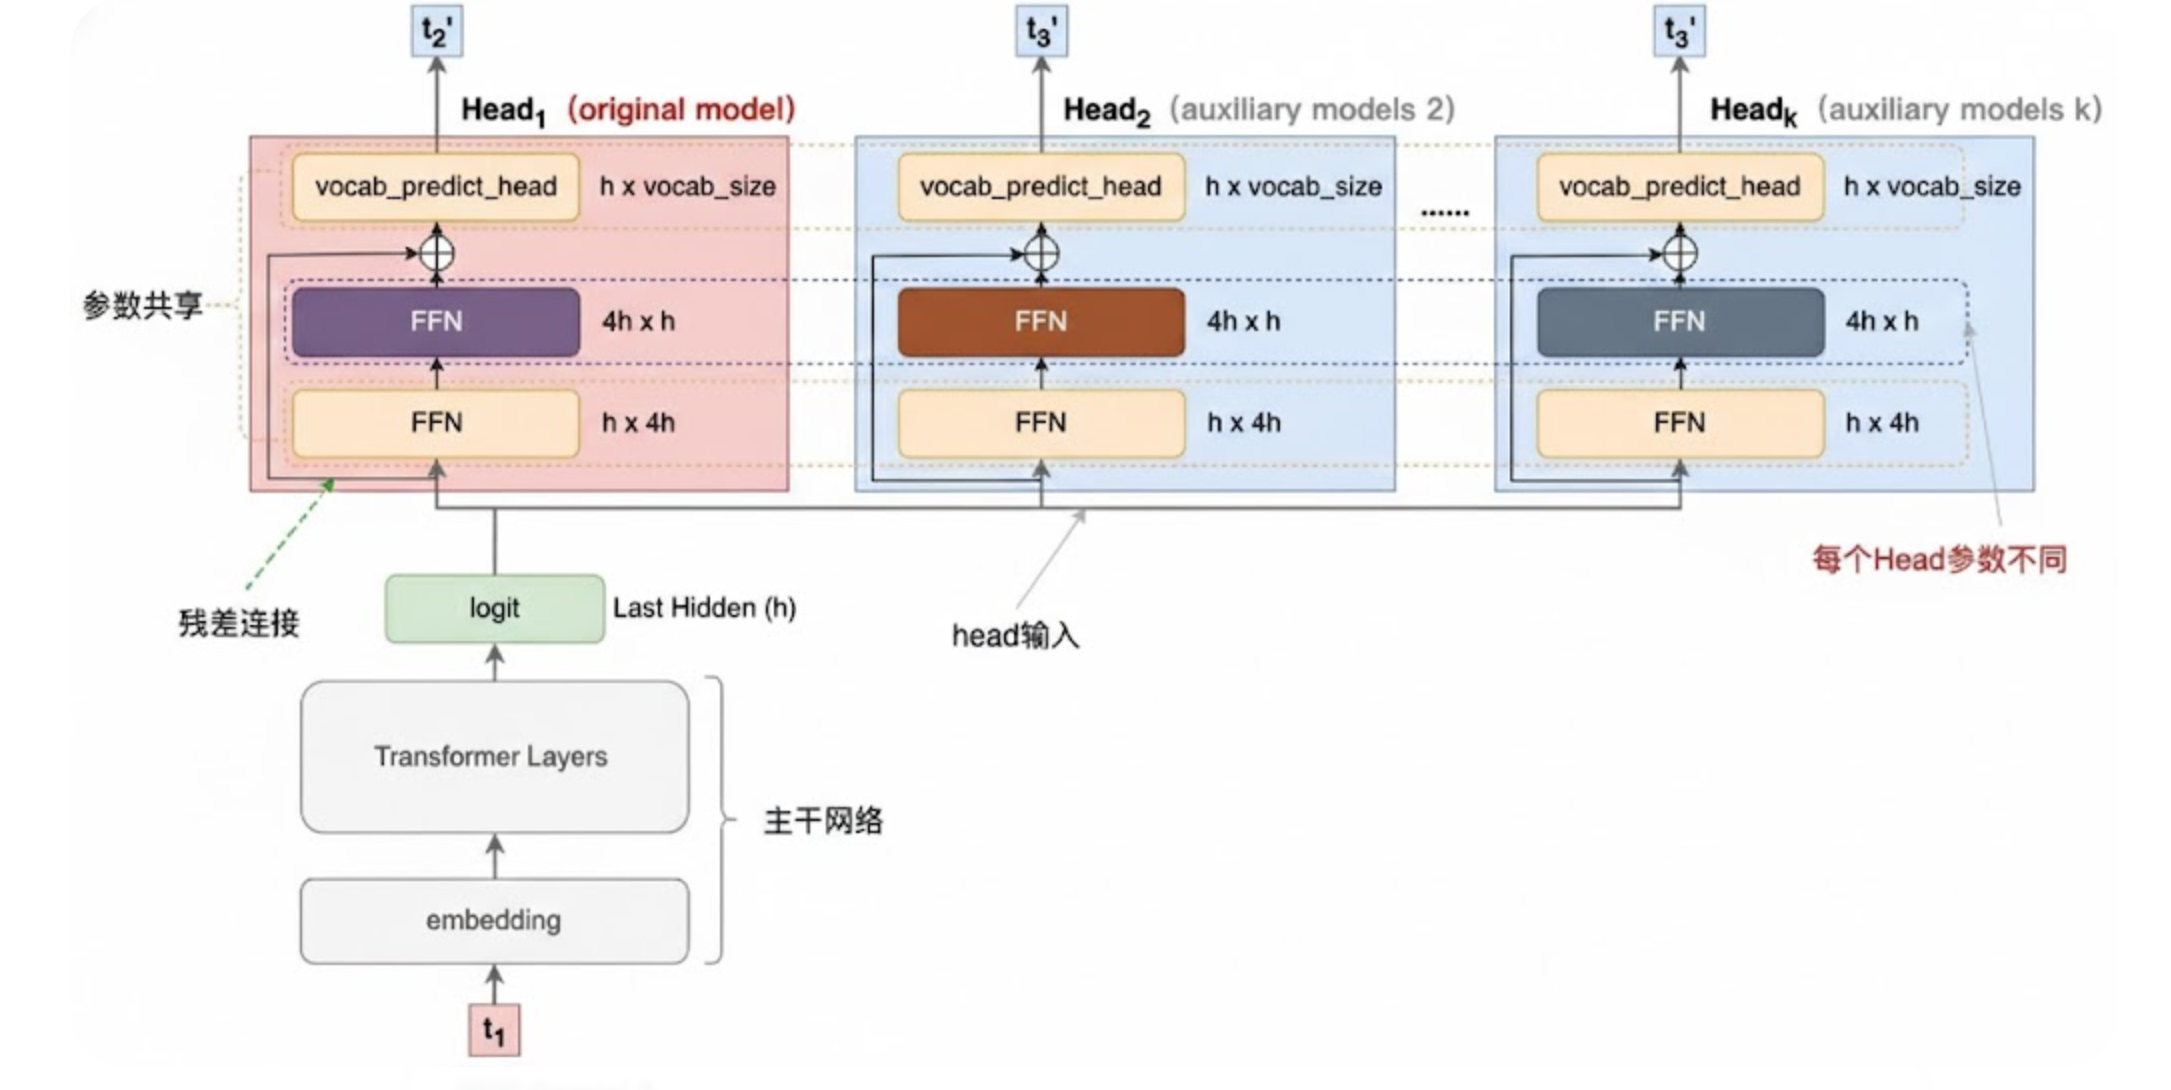
\includegraphics{images/image-0022.png}
\caption{Blockwise Parallel Decoding 模型架构图}
\end{figure}

如图，主干网络是训练好的多层decode-only的Transformer网络，经过多层前向计算后，最终隐藏层输出h维度（＝embedding维度）的logit。上面接了多个输出Head，每个Head负责预估一个token。每个Head有三层：首先是一个共享的FFN层，将logit做宽映射（h维-\textgreater4h维）；然后再过一个非共享的FFN层，将logit维度还原（4h维-\textgreater h维），经残差连接，得到h维embedding向量。最后，再将结果送入到词表投影层得到每个词的概率分布。

\begin{enumerate}
\def\labelenumi{\arabic{enumi}.}
\setcounter{enumi}{1}
\tightlist
\item
  生成范式
\end{enumerate}

\begin{figure}[htbp]
\centering
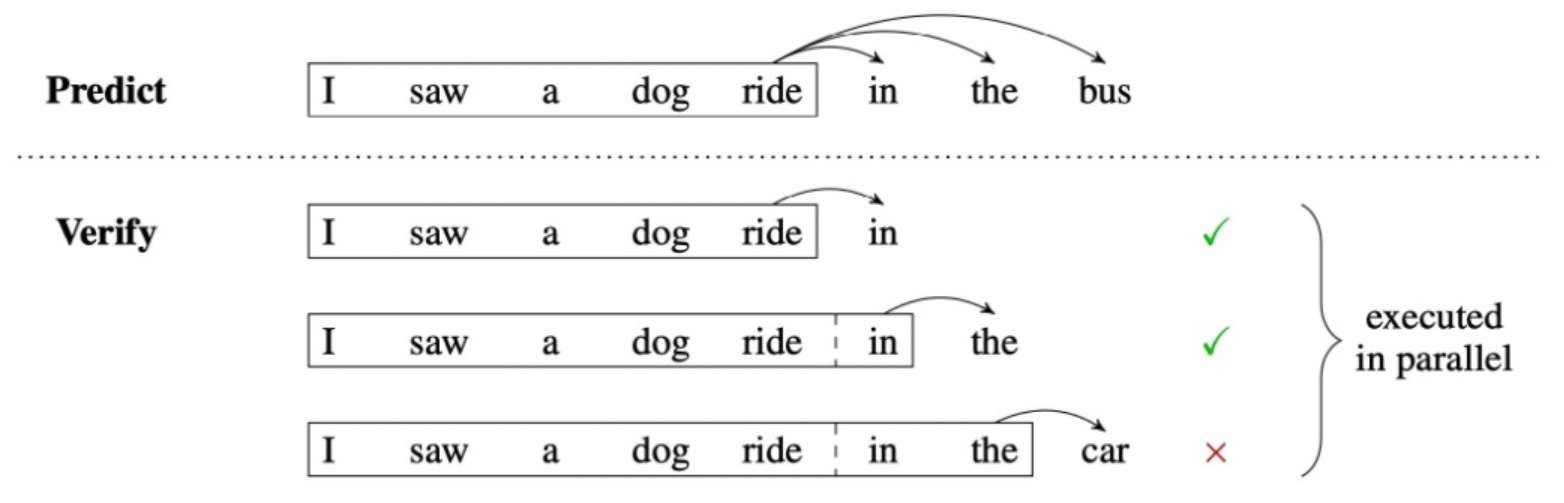
\includegraphics{images/image-0023.png}
\caption{Blockwise Parallel Decoding 的 Predict-Verify 生成与验证流程图}
\end{figure}

MTP的生成过程是一个``Predict-Verify''的循环过程。先一次性预测 \(K\) 个 token，然后利用Transformer的并行性，如图通过掩码的方式实现并行验证。如果预测全部正确，相当于用2次推理的时间实现了 \(K\) 次推理。

进一步地，重叠第 \(n\) 步的 verify 阶段和第 \(n+1\) 步的 predict 阶段，能进一步提高推理性能。如图，先预测出 3 个 token，然后在验证阶段，仍然每次都预测 3 个 token。如由于第 2 个正确，可以以其为条件生成第 3 个``car''、第 4 个``this''和第 5 个``week''，由于最初预测的第 3 个对不上，故最初的预测只能留下``in''和``the''，然后这里生成的第 3 到第 5 个 token 就可以直接作为新的一轮预测，后续再验证此时生成的第 4 和第 5 个，以此类推，不需要重新预测 3 个 token。

\begin{figure}[htbp]
\centering
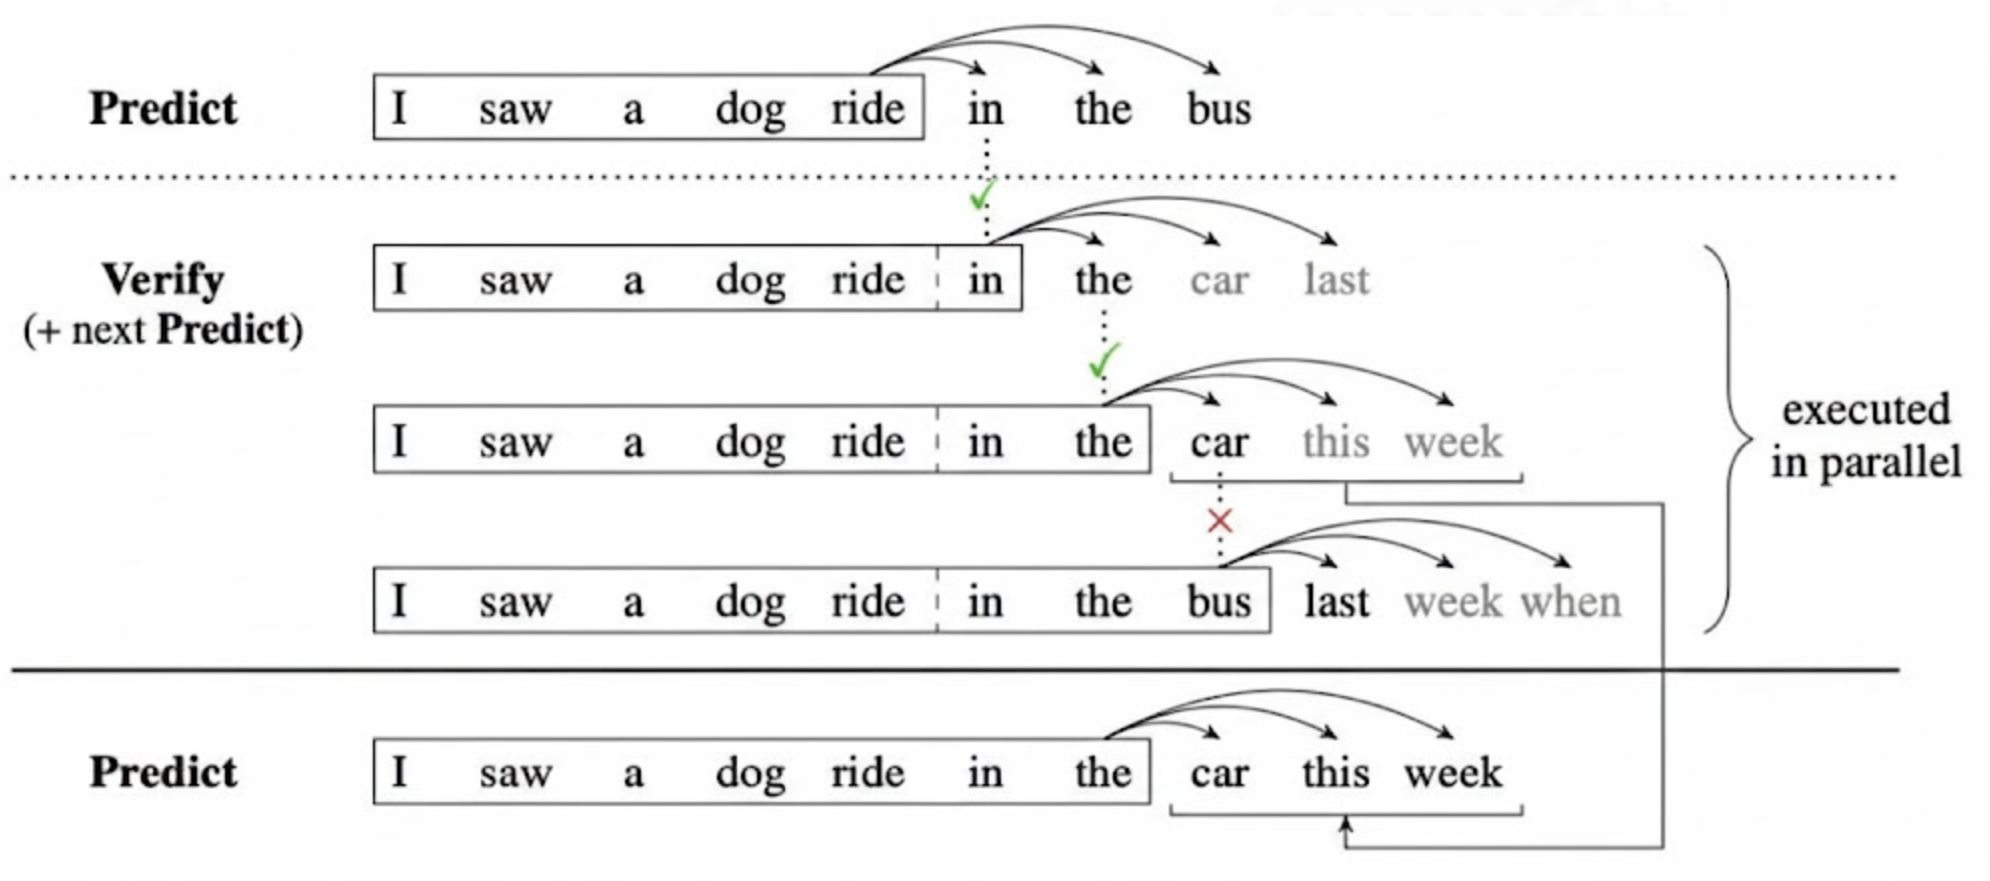
\includegraphics{images/image-0024.png}
\caption{Verify 与下一轮 Predict 重叠执行流程图}
\end{figure}

本质上，这就是利用多token生成的并行性，把后续根据``in''``the''这两个正确的token进行新一轮预测的步骤并入之前的验证步骤。

\hypertarget{ux4e09metas-mtp}{%
\subsection{三、Meta's MTP}\label{ux4e09metas-mtp}}

如图，Meta让每个头不仅仅是FFN层，还有Transformer层，从而可以处理更复杂的序列上下文关系。

\begin{figure}[htbp]
\centering
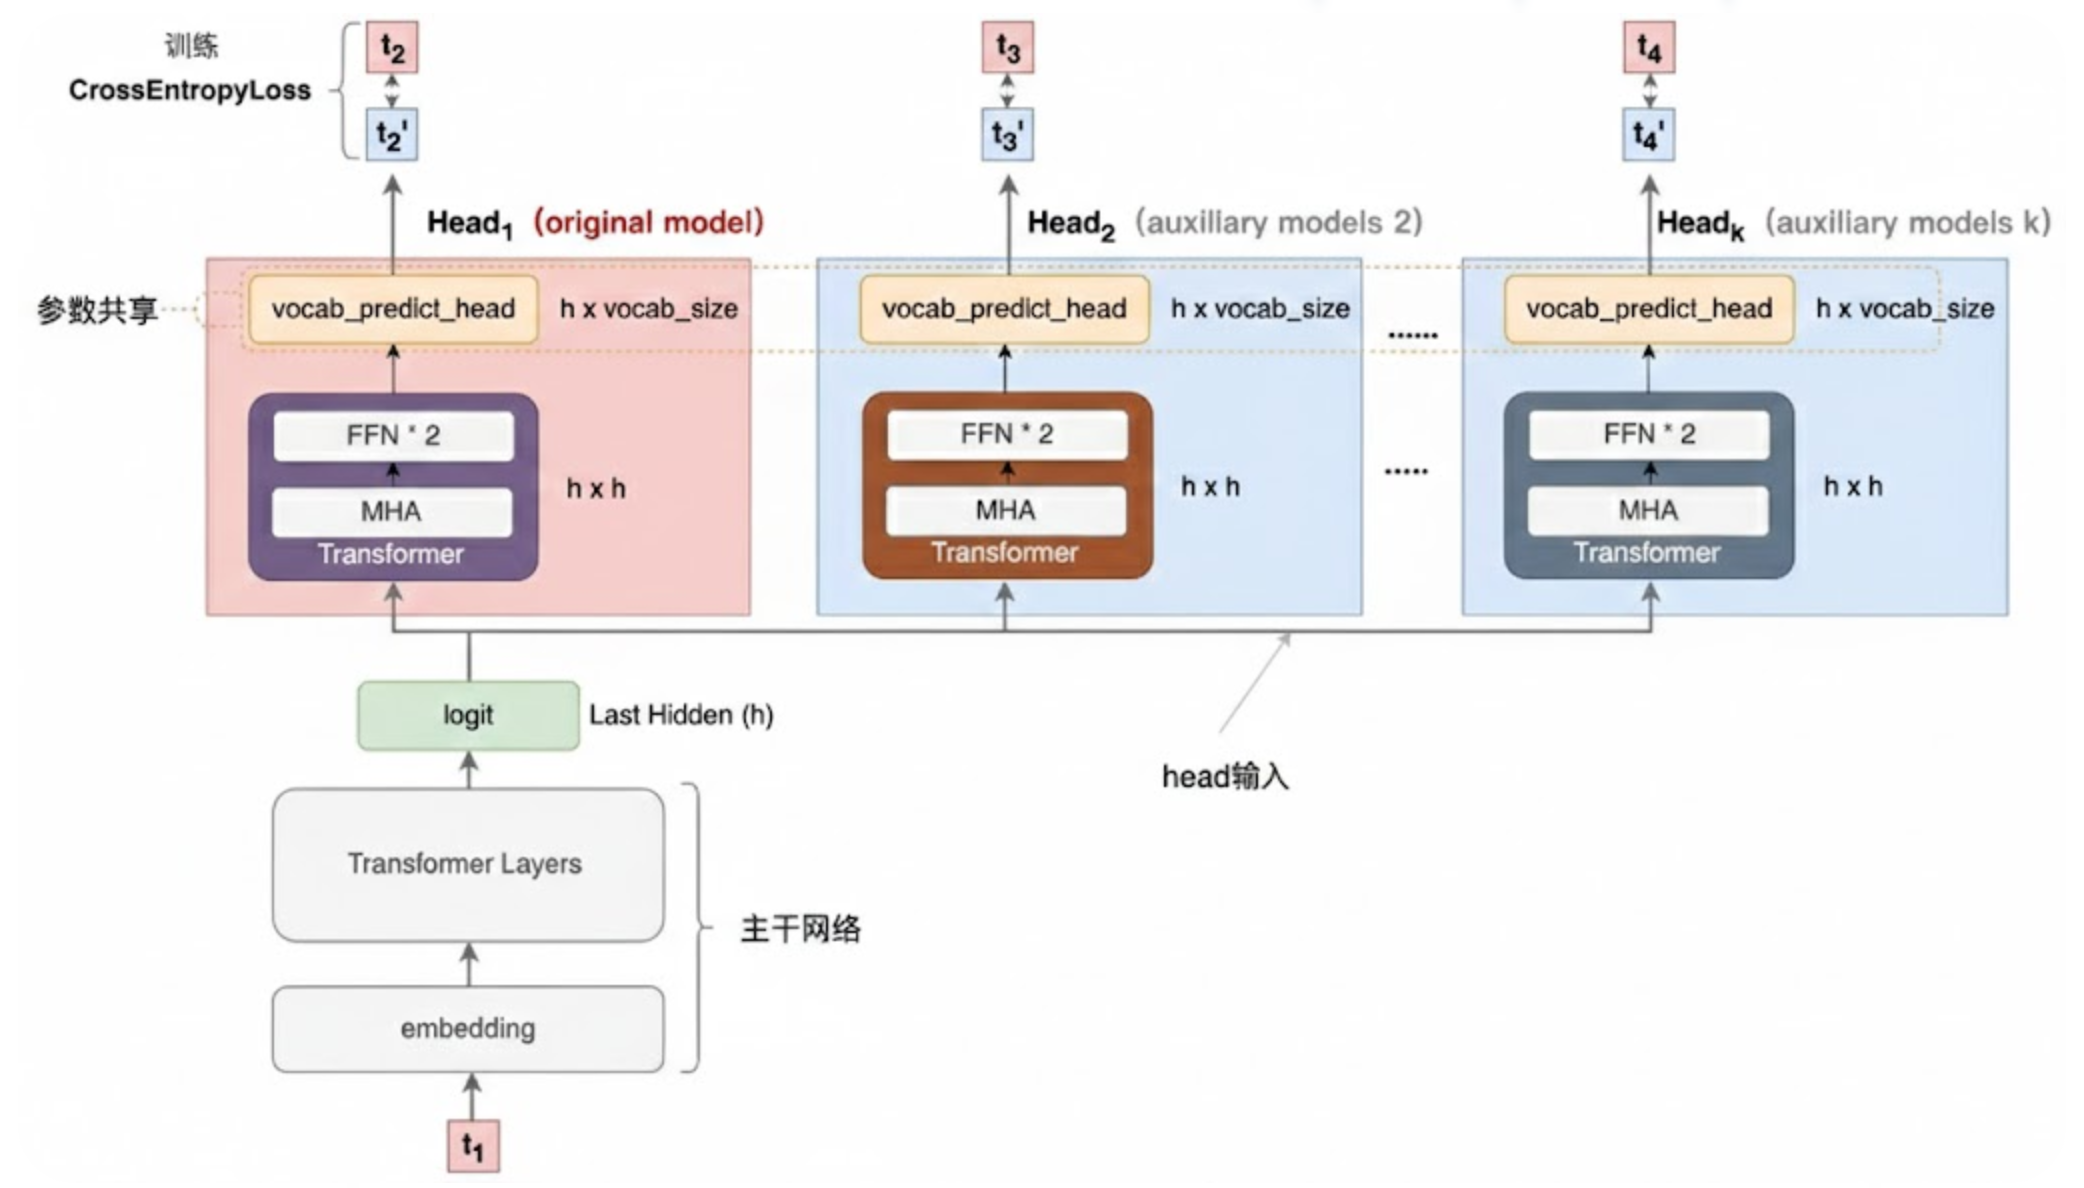
\includegraphics{images/image-0025.png}
\caption{Meta 的 Multi-token Prediction 架构图}
\end{figure}

\hypertarget{ux56dbdeepseek-mtp}{%
\subsection{四、DeepSeek MTP}\label{ux56dbdeepseek-mtp}}

\begin{figure}[htbp]
\centering
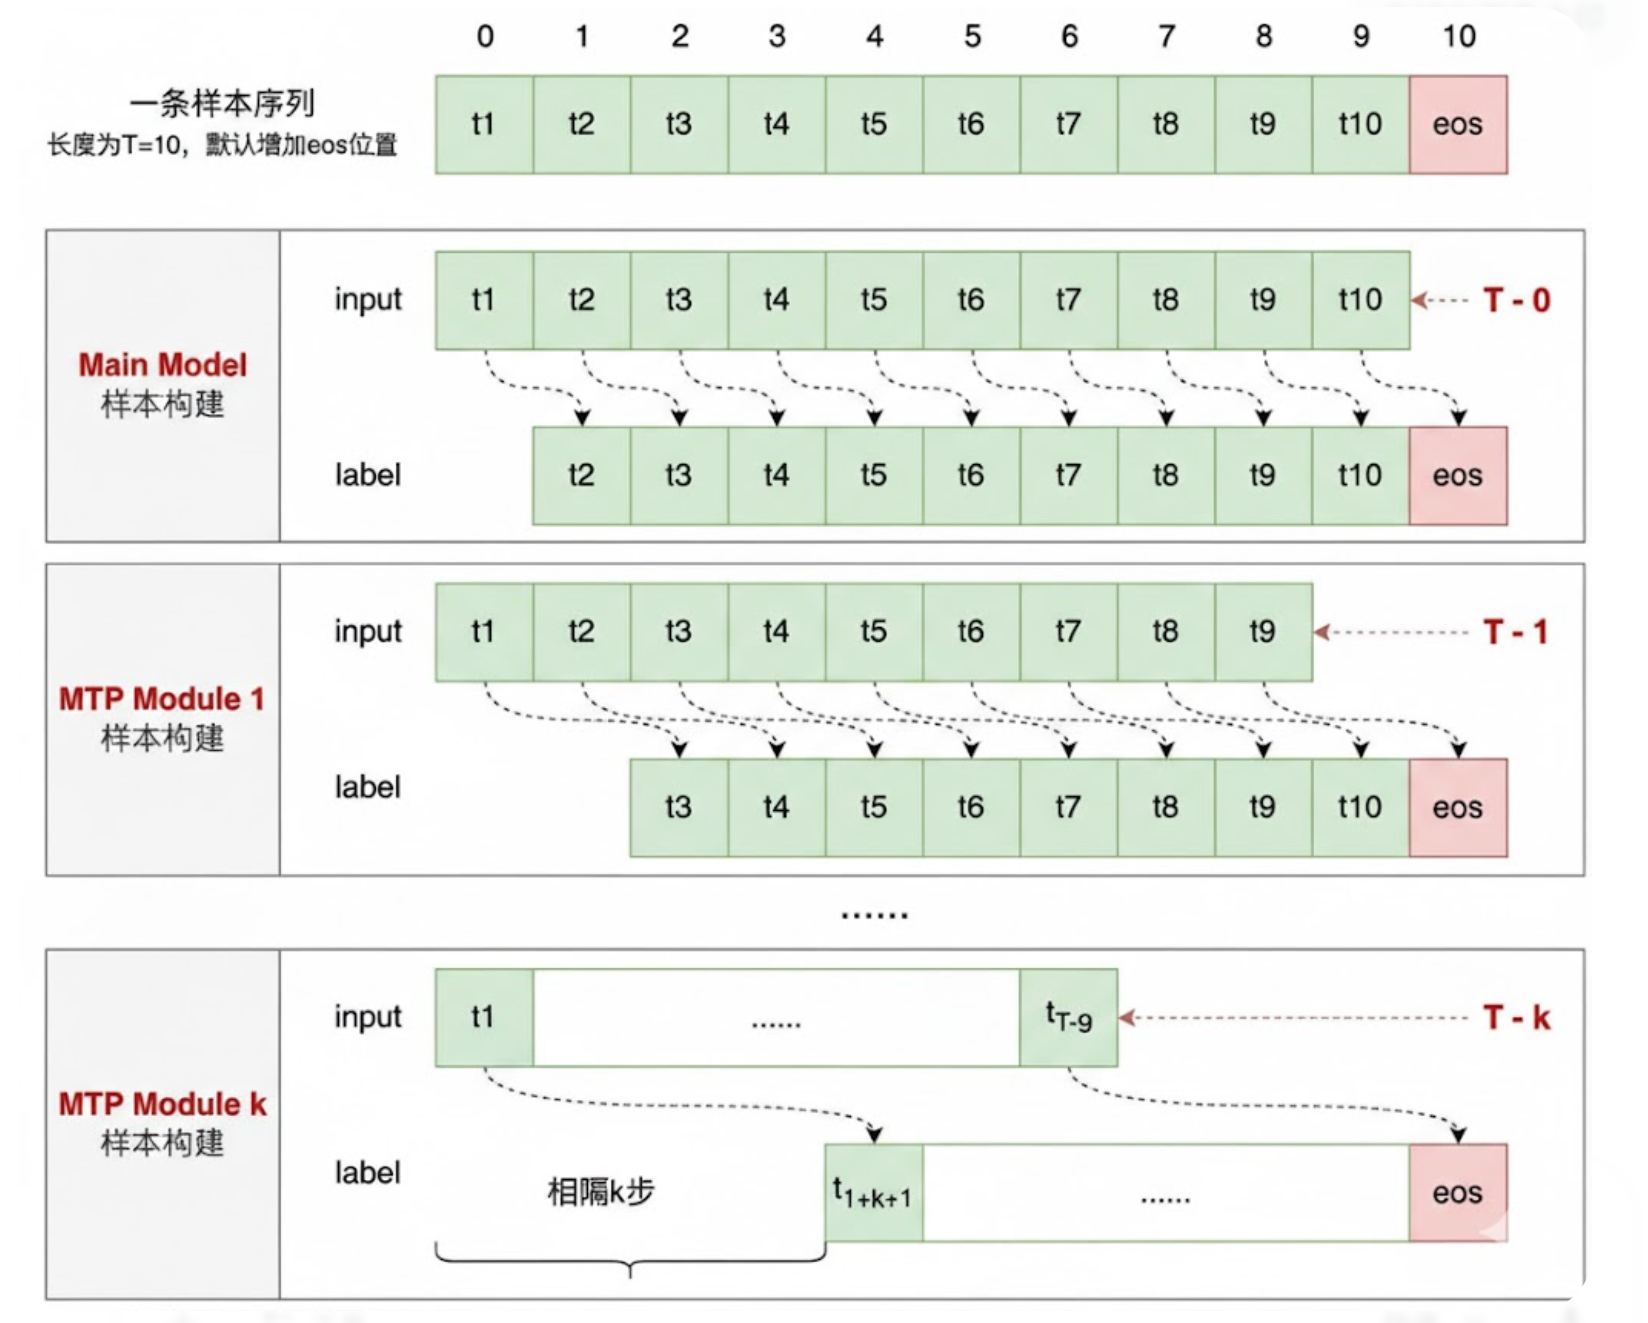
\includegraphics{images/image-0026.png}
\caption{DeepSeek MTP 训练样本构造图}
\end{figure}

训练阶段：Main Model：由 \(t_1\) 生成 \(t_2\)；由 \(t_1,t_2\) 生成 \(t_3\)；\ldots\ldots；由 \(t_1\) 到 \(t_{10}\) 生成 eos token；计算平均Cross-Entropy Loss。MTP Model 1：MTP Module：由 \(t_1,t_2\) 生成 \(t_3\)；\ldots\ldots；由 \(t_1\) 到 \(t_9\) 生成 eos token；计算平均Cross-Entropy Loss。后续的MTP Module以此类推。

\begin{figure}[htbp]
\centering
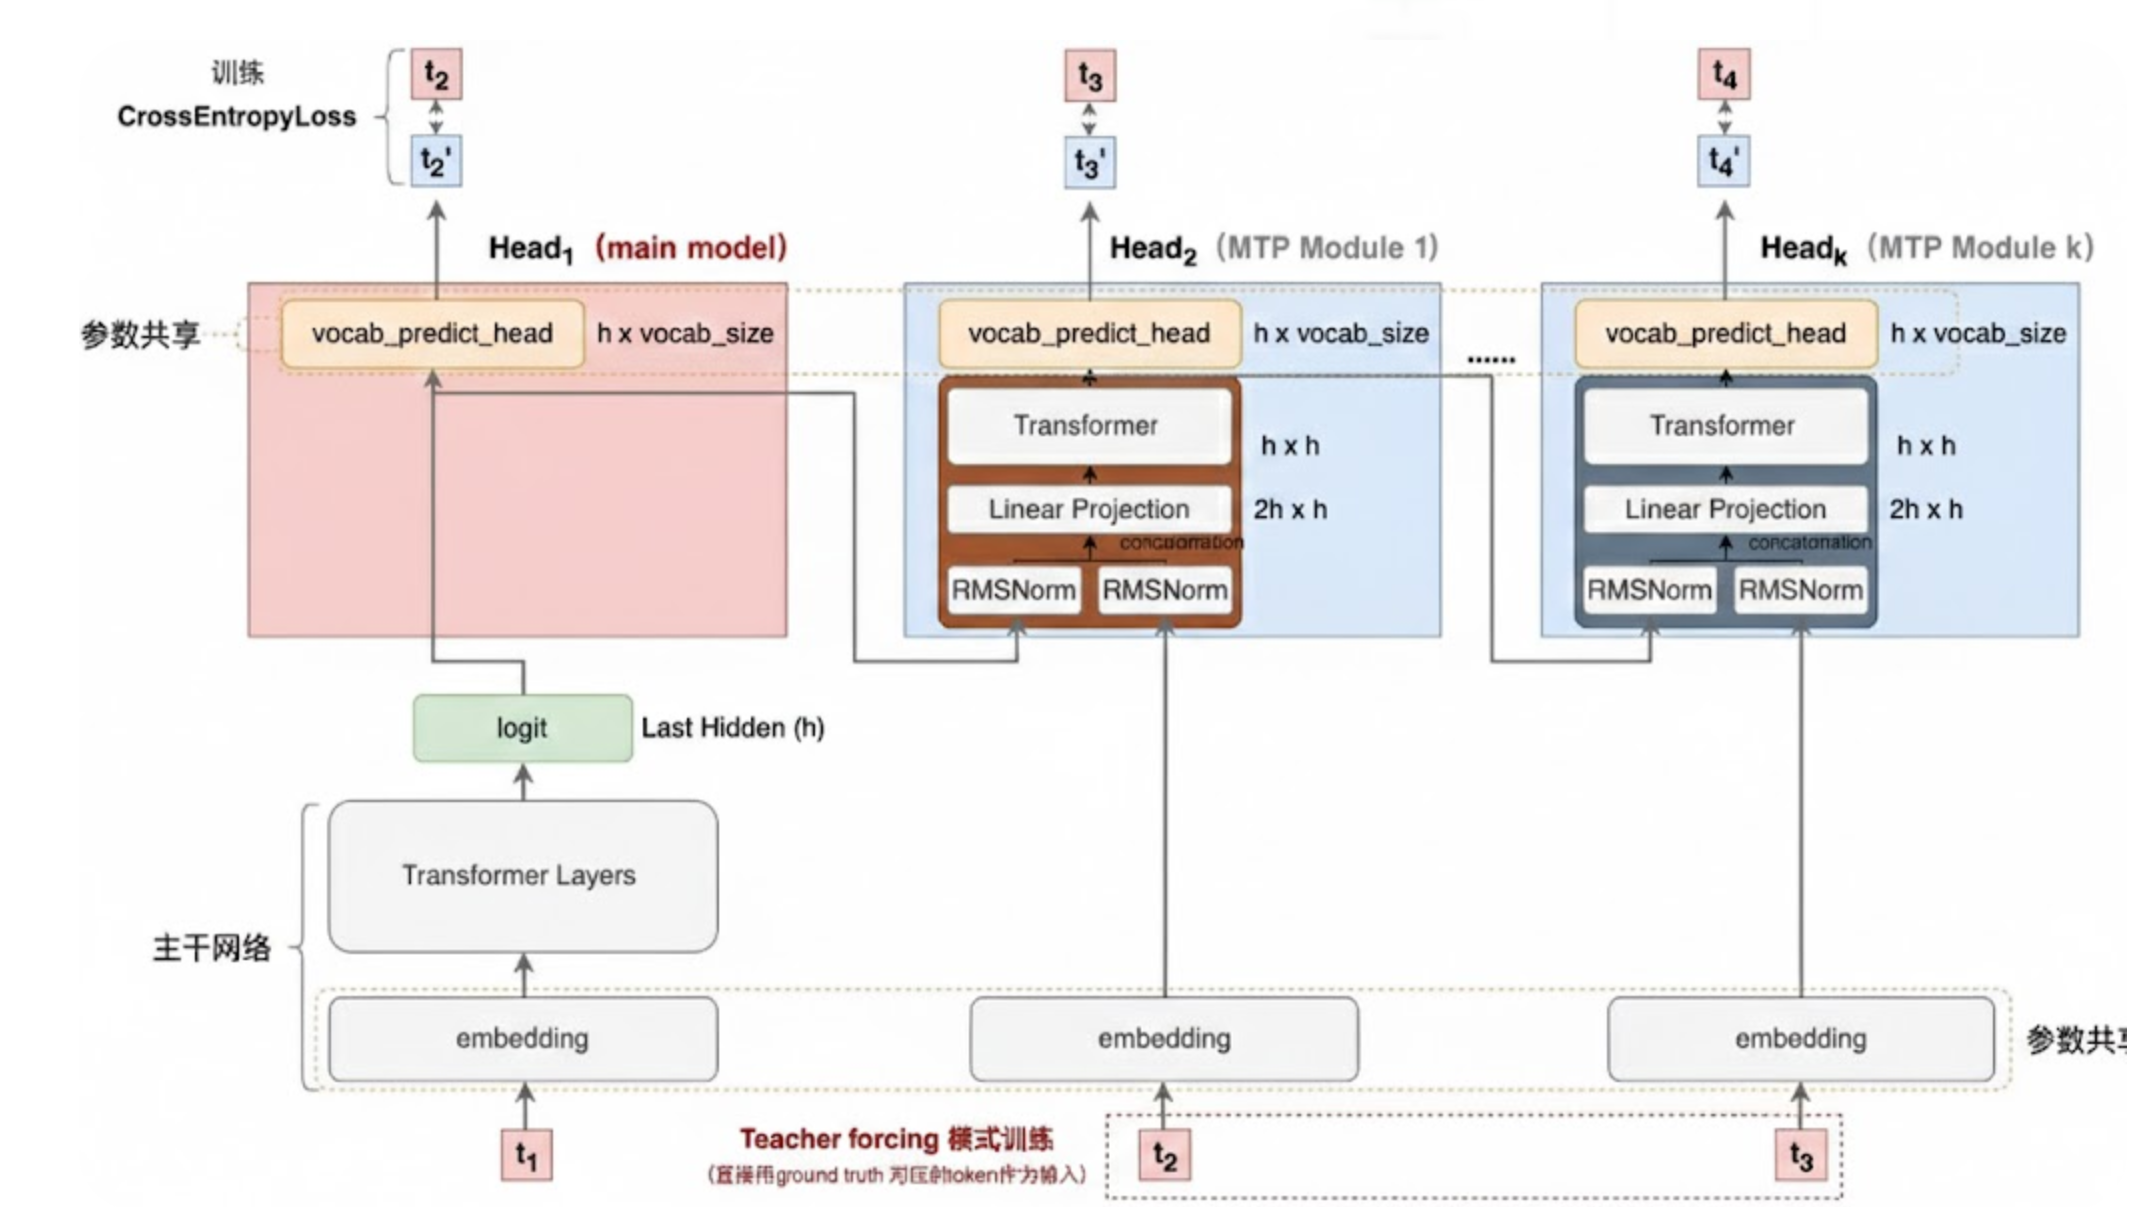
\includegraphics{images/image-0027.png}
\caption{DeepSeek MTP 模块架构图}
\end{figure}

从模型架构上看，DeepSeek在Meta工作的基础上，还在MTP的Transformer层前加上了额外的输入。这个额外输入在训练时是ground truth的t2和t3，以防止细微误差导致``跑偏''；在推理时则是模型自身预测的t2和t3（虽然运用了上一次预测，但这里并非退化为Next token prediction，因为自身预测的t2和t3只经过轻量级MTP模块，不经过全模型，故仍为MTP）。MTP头的损失：

\[
\mathcal{L}_{\mathrm{MTP}}^k
= \mathrm{CrossEntropy}\left(P^k_{2+k:T+1}, t_{2+k:T+1}\right)
= -\frac{1}{T}\sum_{i=2+k}^{T+1}\log P_i^k[t_i].
\]

DeepSeek原论文中插图如下：

\begin{figure}[htbp]
\centering
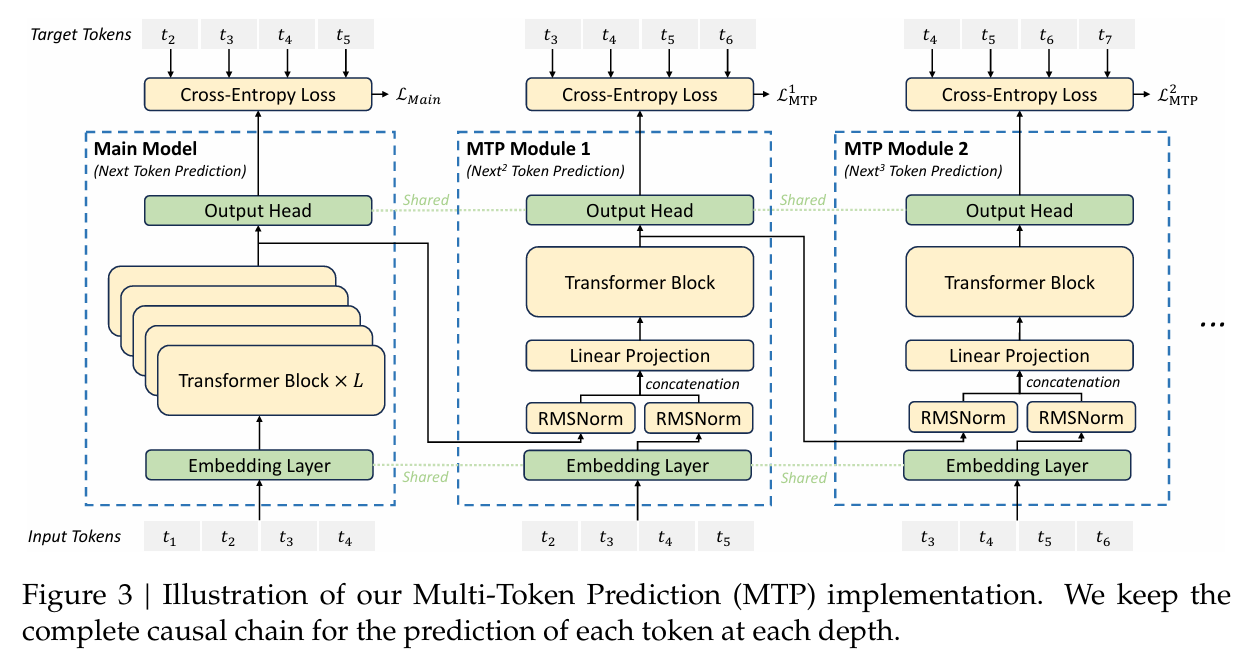
\includegraphics{images/image-0028.png}
\caption{DeepSeek 原论文中的 MTP 模块结构图}
\end{figure}

\hypertarget{ux53c2ux8003ux6587ux732e-99}{%
\subsection{参考文献}\label{ux53c2ux8003ux6587ux732e-99}}

\begin{itemize}
\tightlist
\item
  Stern, M., Shazeer, N., \& Uszkoreit, J. (2018). \href{https://arxiv.org/abs/1811.03115}{Blockwise Parallel Decoding for Deep Autoregressive Models}. NeurIPS 2018.
\item
  Gloeckle, F., Idrissi, B. Y., Roziere, B., et al.~(2024). \href{https://arxiv.org/abs/2404.19737}{Better \& Faster Large Language Models via Multi-token Prediction}. ICML 2024.
\item
  DeepSeek-AI. (2024). \href{https://arxiv.org/abs/2412.19437}{DeepSeek-V3 Technical Report}. arXiv:2412.19437.
\item
  姜富春. (2025). \href{https://zhuanlan.zhihu.com/p/18056041194}{从DeepSeek V3的MTP，解析MTP技术的前世今生}. 知乎专栏.
\end{itemize}

\clearpage

\hypertarget{engramux6a21ux5757ux8bbaux6587}{%
\section{Engram模块（论文）}\label{engramux6a21ux5757ux8bbaux6587}}

\begin{quote}
本文是论文阅读笔记，内容代表对应论文方法或作者理解，不应直接视为领域共识或工程最佳实践。
\end{quote}

传统的大模型架构缺少原生的知识查找方式，只能通过多层计算来低效地模拟检索。如前文为``The capital of France is''时，无法直接查找出``Paris''，只能通过大量参数计算得出。Engram基于条件记忆（Conditional Memory）机制，将记忆（静态知识）与计算（推理能力）解耦，基于哈希查找实现了一种高效率的知识存取方式，从而将更多参数层``腾出来''用于推理。

由于单个token级别的语义记忆在embedding中，跨越上下文的语义通过Attention推理优于直接记忆，故Engram解决的实际上是2-3个token构成的``短语''的记忆问题。

\hypertarget{ux4e00engramux6a21ux5757ux7684ux57faux672cux539fux7406}{%
\subsection{一、Engram模块的基本原理}\label{ux4e00engramux6a21ux5757ux7684ux57faux672cux539fux7406}}

所谓的``静态知识库''实际上是一个长度为S的哈希表，用于存储词组对应的Embedding向量，参数量为S*d\_model。和常见的哈希表初始化为空不同，Engram模块的哈希表初始化时表内的值（参数）均为随机值，后续运用梯度下降更新。研究证明，在模型总参数一定的情况下，除去维度固定的Attention模块外，其余参数20％-30％分配给静态记忆，70％-80％分配给MoE最优。

Engram模块基于NLP中的N-gram方法，N取2和3。推理时，如前文最后三个token为``ABC''时，从哈希表中找2-gram``BC''和3-gram``ABC''对应的几个Engram语义向量，再通过门控机制，按合适的权重加权，加到原向量上。

N取2和3是因为，N=2和N=3覆盖了绝大多数的固定搭配、短语、成语和专有名词（如``New York''``Machine Learning''），这是静态记忆收益最高的区间。N=1对应的是单个词，已经由 Transformer最底层的Embedding Layer完成了，没必要重复存储；N增大，可能的组合呈指数级增长（V\^{}N），但实际在语料中出现的频率却急剧下降，且长序列通常包含复杂的逻辑结构，这部分更适合交给Attention机制动态推导，而不是死记硬背。

\begin{figure}[htbp]
\centering
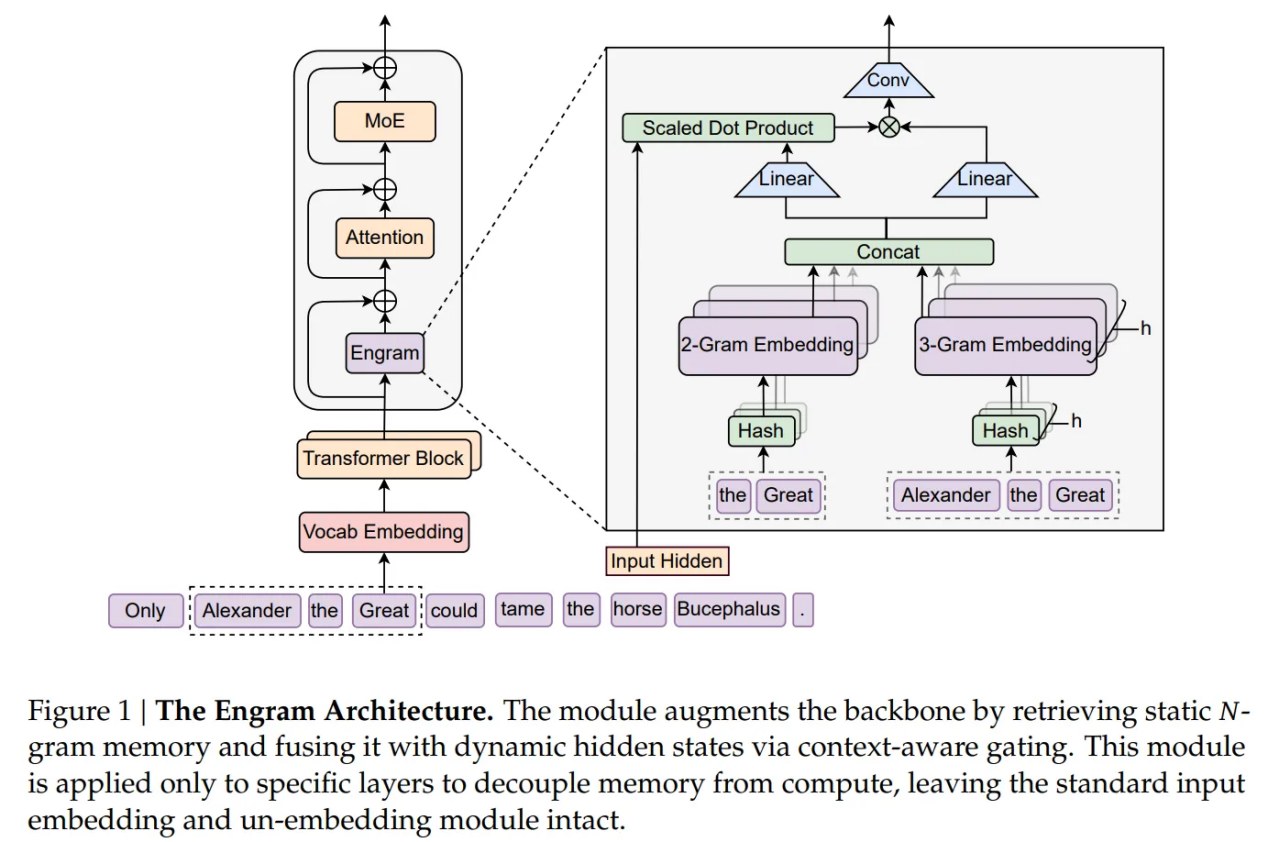
\includegraphics{images/image-0029.png}
\caption{Engram 模块架构图}
\end{figure}

\hypertarget{ux4e8cux54c8ux5e0cux67e5ux627e}{%
\subsection{二、哈希查找}\label{ux4e8cux54c8ux5e0cux67e5ux627e}}

对于输入token序列（为了让查表更紧凑，模型首先将token ID映射到规范形式，如Token ID 105 (``The'')和Token ID 203 (``the'')映射到同一个ID，减少有效词表大小），对于当前第i个token，系统提取其前缀的N-gram，多头哈希函数H\_k计算出K个不同的索引，分别提取这K个位置的Embedding向量。取K个不同的索引是为了缓解哈希冲突，如N-gram A映射到 {[}42, 88{]}，N-gram B映射到 {[}42, 15{]}，42号槽位发生了冲突（Dirty），它混合了A和B的特征，变成了噪声，训练会让模型学会``信任''干净的槽位，而忽略那个冲突的槽位。

如果不用多头，为了避免冲突，必须把表开得非常非常大；使用了多头哈希，可以用一个相对较小（比如S=1亿）的表，容忍一定的碰撞，只要有干净的即可。

\hypertarget{ux4e09ux95e8ux63a7ux673aux5236}{%
\subsection{三、门控机制}\label{ux4e09ux95e8ux63a7ux673aux5236}}

查找得到向量后，将它们与原始输入向量进行门控加和。门控机制类似于一个去掉Softmax的小型Cross-Attention模块，可以根据输入语境确定每个查找到的向量以多大权重聚合进来。由输入向量得到Q、Engram向量矩阵得到K和V，Q和K点乘也就是根据输入决定每个维度的权重分数（这里是独立计算每个向量注入的权重，故不归一化），然后再将每个检索得到的V向量按权重加权得到Engram\_Output向量。最后与原输入向量相加：h\_\{next\} = h\_\{input\} + Engram\_Output。

如输入``capital of France''，模型处于``知识饥渴''状态，查表得到的``Paris''对应向量点积分数高（极大化``Paris''作为下一个词出现的概率），因哈希冲突查到的无关的``Apple''对应向量点积分数低，结果``Paris''相关向量被强力注入，辅助预测；代码推理任务下，所有向量所有维度权重几乎全0，相当于将Engram模块旁路。

\hypertarget{ux56dbux548cux786cux4ef6ux7684ux534fux540cux6027}{%
\subsection{四、和硬件的协同性}\label{ux56dbux548cux786cux4ef6ux7684ux534fux540cux6027}}

\begin{enumerate}
\def\labelenumi{\arabic{enumi}.}
\item
  异步计算和存储：在训练时，为便于反向传播梯度，Engram模块分布在多块GPU上；在推理时，则存储在CPU上，在GPU进行前几层Attention计算时，CPU也在根据输入序列的token ID进行哈希查找，找到N-gram向量，到GPU执行到需要检索的步骤时完成门控嵌入即可。
\item
  分层设计：自然语言中的N-gram 遵循Zipfian分布，即少量高频模式贡献了绝大多数的记忆访问，故可以构建一种多级缓存层次结构（Multi-Level Cache Hierarchy）：将高频访问的嵌入缓存于更快的存储介质中（如GPU HBM或主机DRAM），而将大量低频的长尾模式存放在容量更大但速度较慢的存储介质中（如NVMe SSD）。这种分层设计使Engram能够扩展到极大规模的记忆容量，同时对有效访问延迟的影响保持在最低水平。
\end{enumerate}

\hypertarget{ux53c2ux8003ux6587ux732e-100}{%
\subsection{参考文献}\label{ux53c2ux8003ux6587ux732e-100}}

\begin{itemize}
\tightlist
\item
  Cheng, X., Zeng, W., Dai, D., et al.~(2026). \href{https://arxiv.org/abs/2601.07372}{Conditional Memory via Scalable Lookup: A New Axis of Sparsity for Large Language Models}. arXiv:2601.07372.
\end{itemize}

\clearpage

\hypertarget{ux6d41ux5f62ux5047ux8bbeux4e0eux8d85ux8fdeux63a5}{%
\section{流形假设与超连接}\label{ux6d41ux5f62ux5047ux8bbeux4e0eux8d85ux8fdeux63a5}}

\hypertarget{ux4e00ux6d41ux5f62ux5047ux8bbe}{%
\subsection{一、流形假设}\label{ux4e00ux6d41ux5f62ux5047ux8bbe}}

虽然数据嵌入在一个高维的欧氏空间中，但有意义的数据分布实际上集中在一个维数低得多的低维流形上。也就意味着，对于一个神经网络（或其局部块），从输入x到输出y之间经过的变换是低维的，y-x是分布在低维空间内的向量。

Yoshua Bengio团队在论文《Representation Learning: A Review and New Perspectives》中指出，深度神经网络之所以能泛化，是因为它们成功地学习到了数据所在的低维流形结构，并将其``展开''到了平坦的特征空间中。

\hypertarget{ux4e8cux8d85ux8fdeux63a5hyper-connectionshc}{%
\subsection{二、超连接（Hyper Connections，HC）}\label{ux4e8cux8d85ux8fdeux63a5hyper-connectionshc}}

\hypertarget{ux4e00ux6269ux5c55ux6b8bux5deeux6d41ux5bbdux5ea6}{%
\subsubsection{（一）扩展残差流宽度}\label{ux4e00ux6269ux5c55ux6b8bux5deeux6d41ux5bbdux5ea6}}

在传统的残差神经网络中，y=f(x)+x，f(x)是神经网络主体函数。这里f(x)的输入和输出维度均和x、y的维度相同，均为d\_model。但实际上，f(x)的有效维度应该远小于x、y的表征维度，因此传统的残差神经网络x与y之间的``信息高速公路''太窄，``损失''了很多x、y的有效表征维度，还容易引起网络训练不稳定。

为此，HC将残差流的维度（信息传输维度）和网络主体函数f的维度（计算维度）解耦，加大了残差流的维度，并引入可学习的降维矩阵Hl\_pre和升维矩阵Hl\_post，完成残差流维度和计算维度之间的转换，从而在不显著增大总参数量的前提下，显著增大实际能承载的信息量。

\begin{figure}[htbp]
\centering
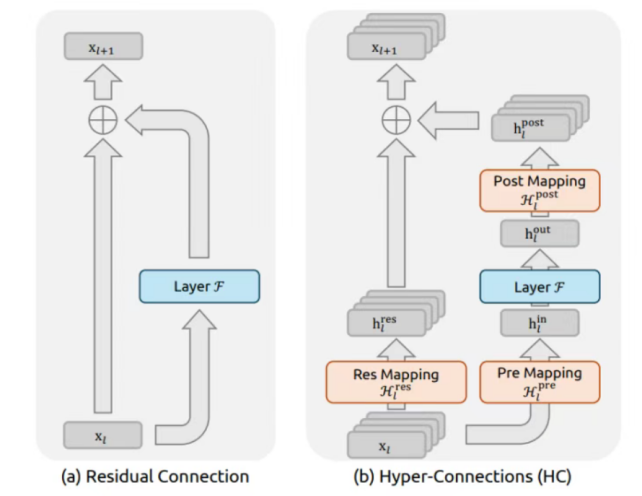
\includegraphics{images/image-0030.png}
\caption{残差连接与超连接结构对比图}
\end{figure}

\hypertarget{ux4e8cux5f15ux5165ux53efux5b66ux4e60ux7684ux6b8bux5deeux8fdeux63a5ux77e9ux9635}{%
\subsubsection{（二）引入可学习的残差连接矩阵}\label{ux4e8cux5f15ux5165ux53efux5b66ux4e60ux7684ux6b8bux5deeux8fdeux63a5ux77e9ux9635}}

从理论上讲，前面的做法已经比较完备了。但HC还引入了残差连接矩阵Hl\_res，对残差流进行线性变换。原因：

\begin{enumerate}
\def\labelenumi{\arabic{enumi}.}
\item
  更好地拟合弯曲流形：深度神经网络由多层构成，对于任意的l，第l层的输出x\_l+1和输入x\_l之差确实都分布在低维空间中，但每一层对应的低维空间的取向往往有一定差异，现实中它们构成的整体流形在高维空间中往往是弯曲的。引入可学习的残差连接矩阵可以让函数的高维空间基底向量灵活地旋转（即不同维度之间可以发生信息交换），增强拟合弯曲流形的性能。
\item
  引入遗忘机制：早期的特征（比如第一层的边缘纹理）在第100层可能已经完全没用了，变成了噪音，但如果不引入Hl\_res，它很难被去除，只能被后面的层通过LayerNorm强行压制，这会浪费宝贵的动态范围。当Hl\_res的特征值小于1时，它起到了遗忘机制的作用。
\end{enumerate}

\hypertarget{ux4e09ux6d41ux5f62ux7ea6ux675fux8d85ux8fdeux63a5}{%
\subsection{三、流形约束超连接}\label{ux4e09ux6d41ux5f62ux7ea6ux675fux8d85ux8fdeux63a5}}

流形约束超连接（Manifold-Constrained Hyper-Connections，mHC）由DeepSeek于2026年提出，是对HC的重要工程化改进。

\hypertarget{ux4e00hcux5b58ux5728ux7684ux95eeux9898}{%
\subsubsection{（一）HC存在的问题}\label{ux4e00hcux5b58ux5728ux7684ux95eeux9898}}

\begin{enumerate}
\def\labelenumi{\arabic{enumi}.}
\item
  数值不稳定：原始的HC中，连接矩阵没有额外的约束，信号在经过多层传播后容易发生梯度爆炸（可达到数百甚至上千倍）或梯度消失，且这还破坏了恒等映射的特性。
\item
  显存和通信开销大：通道变宽意味着显存读写（I/O）和通信成本大幅度增加，即``显存墙''问题。
\end{enumerate}

\hypertarget{ux4e8cmhcux7684ux6539ux8fdb}{%
\subsubsection{（二）mHC的改进}\label{ux4e8cmhcux7684ux6539ux8fdb}}

mHC将变换Hl\_res，Hl\_pre和Hl\_post均限制在了特定的流形上。

\begin{enumerate}
\def\labelenumi{\arabic{enumi}.}
\tightlist
\item
  将Hl\_res限制为双拟随机矩阵
\end{enumerate}

利用Sinkhorn-Knopp 算子，将Hl\_res限制为各元素非负、每行和为1、每列和为1的双拟随机矩阵。本质上说，双拟随机矩阵是排列矩阵的凸组合（排列矩阵：每行、每列只有一个1，其他均为0，一个矩阵乘以排列矩阵，等价于将原矩阵的特征维度向量交换位置），在几何上也就意味着``对于输入向量进行多种旋转（加权）''。它的重复应用会单调地增加跨流的特征融合和信息混合。

此外，该方法在工程上还有两方面优点：

（1）其2-范数有界且不超过1，学习到的映射是非扩张的，可有效缓解梯度爆炸问题。

（2）双拟随机矩阵集对矩阵乘法具有封闭性，确保了跨多层的复合残差映射仍保持双拟随机，从而可在整个模型深度上维持稳定性。

\begin{figure}[htbp]
\centering
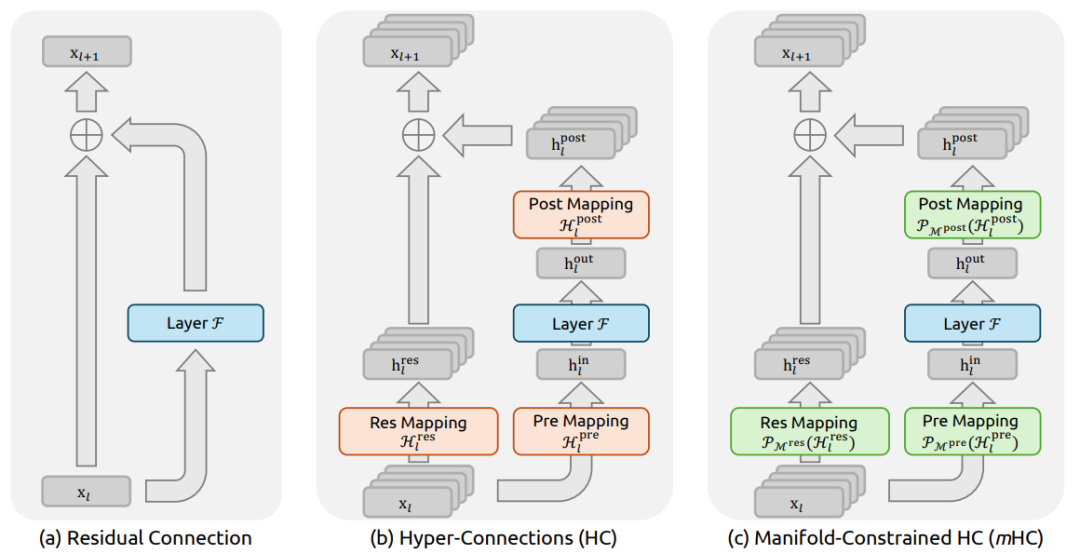
\includegraphics{images/image-0031.png}
\caption{残差连接、超连接与流形约束超连接结构对比图}
\end{figure}

\begin{enumerate}
\def\labelenumi{\arabic{enumi}.}
\setcounter{enumi}{1}
\tightlist
\item
  对Hl\_pre和Hl\_post施加非负约束
\end{enumerate}

Hl\_pre是一个特征重组矩阵，调节各个特征的信号。其第i行第j列的值代表：用于本层计算的低维特征中的第i个维度中，来自高维特征中第j个维度的权重。mHC对两个矩阵均用sigmoid函数转换以保证非负性，提高稳定性，避免正负参数抵消。

注意：这里不用Softmax，因为Softmax要求每行权重之和为1。Hl\_pre如果为10000*1000维，则Softmax会导致输入总信号减小10倍（单个维度信号大小数量级不变，维度除以10）。作为一个门控机制的实现模块，这是不可接受的。

\hypertarget{ux53c2ux8003ux6587ux732e-101}{%
\subsection{参考文献}\label{ux53c2ux8003ux6587ux732e-101}}

\begin{itemize}
\tightlist
\item
  Zhu, D., et al.~(2025). \href{https://arxiv.org/abs/2409.19606}{Hyper-Connections}. arXiv:2409.19606.
\item
  DeepSeek-AI. (2025). \href{https://arxiv.org/abs/2512.24880}{mHC: Manifold-Constrained Hyper-Connections}. arXiv:2512.24880.
\end{itemize}

\clearpage

\hypertarget{attention-residualsux8bbaux6587}{%
\section{Attention Residuals（论文）}\label{attention-residualsux8bbaux6587}}

\begin{quote}
本文是论文阅读笔记，内容代表对应论文方法或作者理解，不应直接视为领域共识或工程最佳实践。
\end{quote}

\hypertarget{ux4e00ux95eeux9898ux80ccux666f-1}{%
\subsection{一、问题背景}\label{ux4e00ux95eeux9898ux80ccux666f-1}}

主流大模型内部的残差连接在每一层处理完信息之后，把处理结果和原来的输入加在一起，传给下一层。每一层做完累加之后，信息就被压进了一个混合状态里。越往后，这个混合状态就越臃肿。随着网络越来越深，混合状态的数值越来越大，发生PreNorm稀释：越深的层，贡献越被稀释。实验证明，一个很深的模型里，删掉相当多的层，效果几乎不变。我们实际上浪费了大量算力。

\hypertarget{ux4e8cux6838ux5fc3ux601dux60f3-1}{%
\subsection{二、核心思想}\label{ux4e8cux6838ux5fc3ux601dux60f3-1}}

目前的主流架构中，每一层的输入=网络输入+前面所有层的输出（等权重）。Kimi团队提出，可以让每一层=网络输入+前面所有层的输出（按需加权求和），权重由这一层自己学。

具体而言，就是用注意力机制，让模型自主决定关注哪些层。每一层有一个自己专属的小向量（只有一个，极其轻量），用它去跟前面所有层的输出算相似度，相似度高的层权重就大，相似度低的权重就小，最后加权求和。值得注意的是，注意力层和MLP层可以关注不同的历史层。

这样，早期层的信息就不会被淹没，可以按需取用。整个改动增加的参数量，相比几十亿参数的大模型来说可以忽略不计，但性能提升到原来的1.25倍，相对于同等性能下节省20％算力。

\hypertarget{ux4e09block-attention-residuals}{%
\subsection{三、Block Attention Residuals}\label{ux4e09block-attention-residuals}}

这种方法的工程问题在于，每一层要关注前面所有层的输出，就必须把前面所有层的输出都存着。现代大模型一般有上百层，训练时还会把模型切成很多份分布到不同机器上（流水线并行），每台机器都要维护所有层的输出，内存压力和通信压力都会暴增。

Kimi的解法是，不用存每一层，改为存每一组。把所有层分成若干个块（block），每个块内部还是用传统方式累加，但把整个块压缩成一个向量存起来。跨块之间，再用注意力机制选择。这样存储量从正比于层数，变成正比于块数。实验发现，分成大约8块就能恢复Full Attention Residuals绝大部分的效果，而内存和通信开销只是原来的一小部分。

\hypertarget{ux53c2ux8003ux6587ux732e-102}{%
\subsection{参考文献}\label{ux53c2ux8003ux6587ux732e-102}}

\begin{itemize}
\tightlist
\item
  Moonshot AI. (2026). \href{https://arxiv.org/abs/2603.15031}{Attention Residuals}. arXiv:2603.15031.
\end{itemize}

\clearpage

\hypertarget{ux81eaux84b8ux998f}{%
\section{自蒸馏}\label{ux81eaux84b8ux998f}}

\hypertarget{ux4e00ux57faux4e8eux4e13ux5bb6ux6f14ux793aux7684ux65b9ux6cd5ux81eaux84b8ux998fux5faeux8c03sdft}{%
\subsection{一、基于专家演示的方法：自蒸馏微调（SDFT）}\label{ux4e00ux57faux4e8eux4e13ux5bb6ux6f14ux793aux7684ux65b9ux6cd5ux81eaux84b8ux998fux5faeux8c03sdft}}

\begin{enumerate}
\def\labelenumi{\arabic{enumi}.}
\tightlist
\item
  提出背景
\end{enumerate}

目前，从专家演示中学习的主流范式是监督微调（SFT）。SFT是Off-policy学习，当模型需要顺序适应新任务或新领域时，SFT会导致严重的泛化能力下降和灾难性遗忘现象。虽然On-policy RL可以显著减少遗忘并提升分布外泛化能力，但它通常需要一个明确的奖励函数。在许多现实世界场景中，构建这样精确的奖励函数是非常困难甚至不可用的。

\begin{enumerate}
\def\labelenumi{\arabic{enumi}.}
\setcounter{enumi}{1}
\tightlist
\item
  核心原理
\end{enumerate}

为了在只有演示或环境反馈数据而没有明确奖励函数的情况下获得同策略学习的优势，自蒸馏让同一个模型在训练中同时扮演``教师''和``学生''两个角色。

学生模型仅接收原始的任务提示词并自回归生成；教师模型接收任务提示词和专家演示，通过大模型的上下文学习能力，每次在学生模型的前 \(i-1\) 个token基础上生成包含正确任务意图的第 \(i\) 个token作为高质量指导信号。

学生模型和教师模型对应的分布可以写为：

\begin{itemize}
\tightlist
\item
  学生模型：在给定前缀 \(y_{<t}\) 和原始问题 \(x\) 的情况下，预测下一个词元的概率分布 \(\pi_\theta(\cdot \mid y_{<t}, x)\)。
\item
  教师模型：在同样前缀下，同时接收专家演示增强提示词 \(c\)，给出更高质量的概率分布 \(\pi(\cdot \mid y_{<t}, x, c)\)。
\end{itemize}

其整体序列级别的逆 KL 散度优化目标为：

\[
\mathcal{L}(\theta)
= D_{\mathrm{KL}}\left(\pi_\theta(\cdot \mid x)\,\Vert\,\pi(\cdot \mid x,c)\right)
= \mathbb{E}_{y\sim \pi_\theta(y\mid x)}
\left[
\log\frac{\pi_\theta(y\mid x)}{\pi(y\mid x,c)}
\right].
\]

式外的期望 \(\mathbb{E}_{y\sim \pi_\theta(y\mid x)}\) 表明，采样的数据分布来自学生策略 \(\pi_\theta\)。

这其实意味着我们是在对整个词汇表V中所有可能的下一个词元v遍历求和：

\[
\nabla_\theta D_{\mathrm{KL}}(\pi_\theta\Vert\pi)
=
\sum_{v\in V}
\pi_\theta(v\mid y_{<t})
\nabla_\theta \log \pi_\theta(v\mid y_{<t})
\left(
\log\frac{\pi_\theta(v\mid y_{<t})}{\pi(v\mid y_{<t},c)}
+ 1
\right).
\]

把每个时间步上的词表求和写成解析梯度估计时，需要保留学生分布的概率权重：

\[
\hat{g}_{\mathrm{analytic}}
=
\sum_{t=1}^{T}\sum_{v\in V}
\pi_\theta(v\mid y_{<t},x)
\nabla_\theta \log \pi_\theta(v\mid y_{<t},x)
\left(
\log\frac{\pi_\theta(v\mid y_{<t},x)}{\pi(v\mid y_{<t},x,c)}
+1
\right).
\]

这在物理意义上等同于：学生模型走到任意一步时，看看在这一步全词表所有可能的选项上，自己的概率分布与教师的概率分布有多大差异，并拉近这种差异。

另外，这里的``专家演示''未必要来自外部，也可以是自身根据后来改出的正确答案。可以类似人类在睡眠时巩固一样，和主进程异步地按自己对同一个问题后来得出的正确答案、优秀经验，对最初上下文较少时的错误输出进行纠正。

\hypertarget{ux4e8cux57faux4e8eux73afux5883ux53cdux9988ux7684ux65b9ux6cd5ux81eaux84b8ux998fux7b56ux7565ux4f18ux5316sdpo}{%
\subsection{二、基于环境反馈的方法：自蒸馏策略优化（SDPO）}\label{ux4e8cux57faux4e8eux73afux5883ux53cdux9988ux7684ux65b9ux6cd5ux81eaux84b8ux998fux7b56ux7565ux4f18ux5316sdpo}}

\begin{enumerate}
\def\labelenumi{\arabic{enumi}.}
\tightlist
\item
  提出背景
\end{enumerate}

RL的训练中，我们通常只会给出一个稀疏的标量结果（如``通过：1''或``未通过：0''），掩盖了底层丰富的状态信息，算法只能把整段代码的所有的词元都进行无差别的梯度惩罚，模型很难弄清楚自己到底错在了哪里------是因为某一行语法写错了、逻辑思辨存在漏洞，还是单纯的边界条件没有处理好。我们希望获得更密集的反馈。

\begin{enumerate}
\def\labelenumi{\arabic{enumi}.}
\setcounter{enumi}{1}
\tightlist
\item
  核心原理
\end{enumerate}

学生模型仅根据原始的指令提示，自回归地生成一个解题尝试。送入可验证环境中执行，环境不仅返回分数，还会输出详细的丰富反馈（如报错信息）。权重相同的教师模型根据原始指令+环境反馈，利用强大的上下文学习能力，在学生模型生成序列的每个位置上，预测下一个词元的正确分布（根据看到的环境反馈得出反思，从而可以纠正学生的错误输出），让学生模型通过最小化KL散度（同前面介绍的反向KL）来逼近这个分布。

\begin{enumerate}
\def\labelenumi{\arabic{enumi}.}
\setcounter{enumi}{2}
\tightlist
\item
  SDPO的好处
\end{enumerate}

相比于奖励信号稀疏的RL，SDPO可以精准地为那一个导致错误的词元计算出巨大的梯度，指导模型只去修正真正犯错的地方。原本仅在序列末尾才有的稀疏且单一的标量奖励，被漂亮地转化为了每一个词元生成时的密集指导信号。理论分析证明，这种机制等价于在最大熵强化学习（Maximum Entropy RL）框架下优化由教师定义的隐式奖励。

这种在PyTorch中仅需调用一次 .forward() 就能算出整条序列密集梯度的设计，不仅避开了off-policy带来的偏移，在显存利用率和计算效率上也远超让两个模型各自生成不同长度序列的传统方法。

\hypertarget{ux53c2ux8003ux6587ux732e-103}{%
\subsection{参考文献}\label{ux53c2ux8003ux6587ux732e-103}}

\begin{itemize}
\tightlist
\item
  Shenfeld, I., Damani, M., Hubotter, J., \& Agrawal, P. (2026). \href{https://arxiv.org/abs/2601.19897}{Self-Distillation Enables Continual Learning}. arXiv:2601.19897.
\item
  Xu, H., et al.~(2026). \href{https://arxiv.org/abs/2601.20802}{Reinforcement Learning via Self-Distillation}. arXiv:2601.20802.
\end{itemize}

\clearpage

\hypertarget{ux591aux4e13ux5bb6on-policy-distillation}{%
\section{多专家On-policy Distillation}\label{ux591aux4e13ux5bb6on-policy-distillation}}

DeepSeek-V4采用了多专家On-policy Distillation的方法，先基于预训练模型，用SFT和RL训练多个领域专家，再将其知识蒸馏到统一的学生模型中。

\hypertarget{ux4e00ux9886ux57dfux4e13ux5bb6ux6a21ux578bux8badux7ec3}{%
\subsection{一、领域专家模型训练}\label{ux4e00ux9886ux57dfux4e13ux5bb6ux6a21ux578bux8badux7ec3}}

基于预训练模型，用SFT和GRPO训练一批领域专家模型，领域包括数学、代码、Agent、指令跟随等。业界一般还会给每个领域训练多种推理强度的子版本，分别对应Non-think、Think、Think Max，三种模式在RL时用不同的length penalty和context window。

做Agent类专家时还引入了~Quick Instruction~机制，聊天产品里有很多附加任务，比如判断是否触发搜索、识别意图。传统做法是另一个小模型做这些，导致每次上下文变化，要重新进行预填充。V4 的做法是给输入序列直接附一组special token，每个token对应一个附加任务，复用现成的KV cache，降低首字延迟。

\hypertarget{ux4e8con-policy-distillation}{%
\subsection{二、On-Policy Distillation}\label{ux4e8con-policy-distillation}}

运用On-Policy蒸馏方法，把所有专家的知识融合到统一的学生模型里。相比于Off-policy方法而言，On-policy更能避免灾难性遗忘。具体而言，即让学生在自己生成的轨迹上学习多个专家模型的输出概率分布。

\hypertarget{ux53c2ux8003ux6587ux732e-104}{%
\subsection{参考文献}\label{ux53c2ux8003ux6587ux732e-104}}

\begin{itemize}
\tightlist
\item
  DeepSeek-AI. (2026). \href{https://huggingface.co/deepseek-ai/DeepSeek-V4-Pro/blob/main/DeepSeek_V4.pdf}{DeepSeek-V4: Towards Highly Efficient Million-Token Context Intelligence}. Technical report.
\end{itemize}

\clearpage

\hypertarget{klux6563ux5ea6ux4e0ejsdux6563ux5ea6}{%
\section{KL散度与JSD散度}\label{klux6563ux5ea6ux4e0ejsdux6563ux5ea6}}

在大模型中，KL散度衡量输出概率分布的差异，并非按输出前的隐藏层维度计算，而是在大小为 \(V\) 的词表上计算（因为本质上大模型的输出是离散的tokens）。

\[
D(P\Vert Q)=\sum_{i=1}^{V}p_i\log\frac{p_i}{q_i}
\]

注意：计算困惑度时是对序列中的所有token的概率负对数取平均，而计算KL散度时是在输出一个token时，对词表中的所有词的KL散度取平均，二者取平均的方式不同。

实际研究中，为了让数值更稳定，往往用KL散度的变体------JSD散度，即取 \(P\) 和 \(Q\) 的平均 \(M\)：

\[
M=\frac{1}{2}(P+Q)
\]

JSD散度定义为：

\[
\mathrm{JSD}(P,Q)=\frac{1}{2}\left(D_{\mathrm{KL}}(P\Vert M)+D_{\mathrm{KL}}(Q\Vert M)\right)
\]

其功能和KL类似但不会出现 \(\log\) 内分母为零，例如研究模型中间隐藏层和输出层之间神经元激活值的JSD散度（如果二者维度不同，则投影后再用JSD散度），就可以判断二者分布之间的相似程度大小。

对于LLM，自回归输出 \(n\) 个token的KL散度：

\[
D_{\mathrm{KL}}(P(Y)\Vert Q(Y))
=
\sum_Y P(Y)\log\frac{P(Y)}{Q(Y)}.
\]

由于直接对所有可能的序列求和是不可行的（有 \(V^n\) 种可能），需利用自回归特性将其分解：

\[
D_{\mathrm{KL}}(P(Y)\Vert Q(Y))
=
\mathbb{E}_{Y\sim P}
\left[
\sum_{t=1}^{n}
\left(
\log P(y_t\mid y_{<t})-\log Q(y_t\mid y_{<t})
\right)
\right]
=
\sum_{t=1}^{n}
\mathbb{E}_{Y\sim P}
\left[
\log\frac{P(y_t\mid y_{<t})}{Q(y_t\mid y_{<t})}
\right].
\]

这里的处理难点在于 \(Y\sim P\)，需要考虑整个序列的概率分布。注意到右边的条件概率的条件为 \(y_{<t}\)，对于给定已知的 \(y_{<t}\) 分布，由自回归特性，\(y_t\) 的分布也会随之确定，\(Y=\{y_1,\ldots,y_t\}\) 的分布也就已知。因此可以改写为：

\[
D_{\mathrm{KL}}(P(Y)\Vert Q(Y))
=
\sum_{t=1}^{n}
\mathbb{E}_{y_{<t}\sim P(y_{<t})}
\left[
D_{\mathrm{KL}}\left(P(y_t\mid y_{<t})\Vert Q(y_t\mid y_{<t})\right)
\right].
\]

这意味着，两个序列分布的KL散度，等于每一步条件概率分布之间KL散度的期望之和（期望是基于分布 \(P\) 生成的历史轨迹计算的）。

\hypertarget{ux53c2ux8003ux6587ux732e-105}{%
\subsection{参考文献}\label{ux53c2ux8003ux6587ux732e-105}}

\begin{itemize}
\tightlist
\item
  Kullback, S., \& Leibler, R. A. (1951). \href{https://doi.org/10.1214/aoms/1177729694}{On Information and Sufficiency}. The Annals of Mathematical Statistics, 22(1), 79-86.
\item
  Lin, J. (1991). \href{https://doi.org/10.1109/18.61115}{Divergence measures based on the Shannon entropy}. IEEE Transactions on Information Theory, 37(1), 145-151.
\end{itemize}

\clearpage

\hypertarget{ux56f0ux60d1ux5ea6}{%
\section{困惑度}\label{ux56f0ux60d1ux5ea6}}

困惑度（Perplexity, PPL）是评估语言模型好坏的黄金指标。它的核心思想是：一个好的模型，应该对真实的下一个词赋予很高的预测概率。模型越感到``困惑''，它的预测就越不准，困惑度的值就越高。

\hypertarget{ux4e00ux76f4ux89c2ux7406ux89e3}{%
\subsection{一、直观理解}\label{ux4e00ux76f4ux89c2ux7406ux89e3}}

假设一个完美的语言模型，它总是能 100\% 确定下一个词是什么（即预测概率为 \(1\)）。那么它的困惑度是 \(\exp(0)=1\)。这意味着模型毫不困惑，等价于它每次只有 1 个词的选择（就是那个正确的词）。

一个非常差的模型，比如它总是认为词表中的所有 10 万个词都是等可能的（每个词概率为 \(1/100000\)）。那么它的困惑度就是 100000。这意味着模型非常困惑，等价于它每次都要在 10 万个词里做选择。

一个好的模型的困惑度应该介于 1 和词表大小之间。例如，在 WikiText-2 数据集上，现代模型的困惑度可以降到 20 左右。这意味着每次模型平均是从 20 个词中选一个，比较``确定''接下来会发生什么。

\hypertarget{ux4e8cux6570ux5b66ux8868ux8fbeux4e0eux63a8ux5bfc}{%
\subsection{二、数学表达与推导}\label{ux4e8cux6570ux5b66ux8868ux8fbeux4e0eux63a8ux5bfc}}

困惑度与信息论中的交叉熵（Cross-Entropy）~紧密相关。交叉熵衡量的是模型预测的概率分布与真实的概率分布（这里其实是one-hot分布，即真实词的概率为1，其他为0）之间的差异。事实上，交叉熵损失函数取指数后，就可以视为整个序列的困惑度（``生成该序列时，每次平均从几个token里选一个''）。困惑度的n次方的倒数就是生成该序列的联合概率，最小化困惑度（PPL）在数学上完全等价于最大化模型分配给整个序列的联合概率。

数学推导：

\begin{enumerate}
\def\labelenumi{\arabic{enumi}.}
\tightlist
\item
  起点：序列概率
\end{enumerate}

语言模型的目标是给真实序列 \(W=(w_1,w_2,\ldots,w_N)\) 赋予高概率。根据链式法则，这个概率是所有条件概率的乘积：

\[
P(W)=P(w_1)\prod_{t=2}^{N}P(w_t\mid w_1,\ldots,w_{t-1})
\]

\begin{enumerate}
\def\labelenumi{\arabic{enumi}.}
\setcounter{enumi}{1}
\tightlist
\item
  取对数（为了将连乘变为求和）
\end{enumerate}

直接优化乘积在数学上很麻烦（可能下溢），我们取对数，转化为对数似然（Log-Likelihood）。因为对数函数是单调的，最大化概率乘积等价于最大化对数似然和。

\[
\log P(W)=\log P(w_1)+\sum_{t=2}^{N}\log P(w_t\mid w_1,\ldots,w_{t-1})
\]

\begin{enumerate}
\def\labelenumi{\arabic{enumi}.}
\setcounter{enumi}{2}
\tightlist
\item
  取平均（为了消除长度影响）
\end{enumerate}

为了比较不同长度序列的性能，我们取平均值，得到平均对数似然。

\[
\frac{1}{N}\log P(W)
\]

\begin{enumerate}
\def\labelenumi{\arabic{enumi}.}
\setcounter{enumi}{3}
\tightlist
\item
  取负号（为了得到损失）
\end{enumerate}

我们习惯最小化一个``损失''函数，而不是最大化一个``得分''函数。因此我们取负值，得到平均负对数似然。这个值越低越好。

\[
L=-\frac{1}{N}\log P(W)
\]

\begin{enumerate}
\def\labelenumi{\arabic{enumi}.}
\setcounter{enumi}{4}
\tightlist
\item
  困惑度的定义
\end{enumerate}

困惑度被定义为这个平均负对数似然的指数：

\[
\mathrm{PPL}=\exp(L)=\exp\left(-\frac{1}{N}\log P(W)\right)
\]

根据指数法则，上式可以重写为：

\[
\mathrm{PPL}=P(W)^{-1/N}
=\left[P(w_1)\prod_{t=2}^{N}P(w_t\mid w_1,\ldots,w_{t-1})\right]^{-1/N}
\]

\begin{enumerate}
\def\labelenumi{\arabic{enumi}.}
\setcounter{enumi}{5}
\tightlist
\item
  与概率的关系
\end{enumerate}

让 \(P(W)^{1/N}\) 变大，就是让序列的平均几何概率变大。因此，最小化困惑度（PPL）在数学上严格等价于最大化整个序列的联合概率 \(P(W)\)。

\hypertarget{ux4e09ux4fe1ux606fux8bbaux89e3ux91ca}{%
\subsection{三、信息论解释}\label{ux4e09ux4fe1ux606fux8bbaux89e3ux91ca}}

第一步：理解``取对数''的意义------衡量惊讶度

在信息论中，\(-\log_2 P(\mathrm{event})\) 衡量的是事件的``惊讶度（Surprisal）''或``信息量''。

如果一个事件必然发生（概率 \(P=1\)），它的惊讶度为 \(-\log_2 1=0\) 比特。你毫不惊讶。

如果一个事件非常罕见（概率 \(P\to 0\)），它的惊讶度趋近于无穷大。你极度惊讶。

如果一个事件有 50\% 的概率发生（\(P=0.5\)），它的惊讶度是 \(-\log_2 0.5=1\) 比特。

在语言模型中，\(-\log P(w_t\mid \mathrm{context})\) 衡量的是：当真实的下一个词 \(w_t\) 出现时，模型感到有多``惊讶''。概率越低，惊讶度越高。

所以，平均负对数似然~L：

\[
L=\frac{1}{N}\sum_{t=1}^{N}-\log P(w_t\mid w_{<t})
\]

它的物理意义是：模型在预测序列中每个词时，平均的``惊讶程度''（单位：比特/词）。

第二步：理解``取指数''的意义------回到选择空间
我们现在有了一个``平均惊讶度''（比如 6.5 比特/词）。但这个数字对我们来说不够直观。6.5 比特的惊讶到底有多惊讶？

若 \(L\) 使用自然对数，则 \(\exp(L)\) 操作的核心作用是将``惊讶度''重新转换回``概率空间''；若 \(L\) 使用以 2 为底的对数，则对应的转换是 \(2^L\)。更具体地说，它把平均惊讶度转换回一个等价的均匀分布选择问题。

让我们看一个例子：

假设有一个非常差劲的模型，它对下一个词的预测完全随机，词表 \(|V|\) 有 1024 个词。那么它对每个词的预测概率都是 \(1/1024\)。

每个词的惊讶度：

\[
-\log_2(1/1024)=\log_2(1024)=10
\]

平均惊讶度 \(L\) 也是 10 比特/词。

计算困惑度：

\[
\mathrm{PPL}=2^L=2^{10}=1024
\]

这里有一个关键点：信息论中 \(\log\) 底数常取 2，但数学计算中常用自然对数（底数为 \(e\)）。二者只差一个常数因子，只要前后一致即可。这个最差模型的困惑度正好等于词表大小 1024。

这可以解释为：这个模型在预测每个词时，其表现就好像它在一个均匀分布的、包含1024个候选词的词表中进行盲猜一样。~它的不确定性等同于做1024选1的选择。

再举一个例子：假设一个好模型用自然对数计算出的平均负对数似然是 \(L=\log 64\)（约等于 4.16）。

计算困惑度：

\[
\mathrm{PPL}=\exp(L)=\exp(\log 64)=64
\]

这可以解释为：虽然真实的词表可能有成千上万个词，但这个模型的能力非常强，它在预测每个词时，其不确定性平均只相当于在一个仅有64个候选词的小集合里做选择。

\hypertarget{ux53c2ux8003ux6587ux732e-106}{%
\subsection{参考文献}\label{ux53c2ux8003ux6587ux732e-106}}

\begin{itemize}
\tightlist
\item
  Jurafsky, D., \& Martin, J. H. (2026). \href{https://web.stanford.edu/~jurafsky/slp3/3.pdf}{Speech and Language Processing, Chapter 3: N-gram Language Models}. Draft of January 6, 2026.
\item
  Brown, P. F., Della Pietra, V. J., deSouza, P. V., Lai, J. C., \& Mercer, R. L. (1992). \href{https://aclanthology.org/J92-4003/}{Class-Based n-gram Models of Natural Language}. Computational Linguistics, 18(4), 467-480.
\end{itemize}

\clearpage


% 强化微调的前沿探索
\hypertarget{ux5f3aux5316ux5faeux8c03ux7684ux524dux6cbfux63a2ux7d22}{%
\chapter{强化微调的前沿探索}\label{ux5f3aux5316ux5faeux8c03ux7684ux524dux6cbfux63a2ux7d22}}

\hypertarget{dapoux7b97ux6cd5ux8bbaux6587}{%
\section{DAPO算法（论文）}\label{dapoux7b97ux6cd5ux8bbaux6587}}

\begin{quote}
本文是论文阅读笔记，内容代表对应论文方法或作者理解，不应直接视为领域共识或工程最佳实践。
\end{quote}

DeepSeek的成功证明了GRPO范式的有效性和优越性。但是，GRPO仍然存在稳定性问题，容易导致训练崩溃。DeepSeek拥有足够多的数据，可以使其趋于稳定。但对于中小规模的强化微调，如果数据批量较小，就必须对算法本身进行改进。

DAPO（Decoupled Clip and Dynamic Sampling Policy Optimization）就是其中一种改进，它基本上沿用了GRPO的算法原理，但做出了一些工程策略上的改进。

\hypertarget{ux4e00ux6539ux8fdbux70b9}{%
\subsection{一、改进点}\label{ux4e00ux6539ux8fdbux70b9}}

\begin{enumerate}
\def\labelenumi{\arabic{enumi}.}
\tightlist
\item
  Clip-Higher 机制（解耦 Clip）
\end{enumerate}

这是 DAPO 最显著的数学改进。

\begin{itemize}
\tightlist
\item
  \textbf{原理}：传统 PPO/GRPO 使用对称的裁剪范围 \((1-\epsilon, 1+\epsilon)\)。DAPO 将上界和下界解耦，设为 \((1-\epsilon_{\mathrm{low}}, 1+\epsilon_{\mathrm{high}})\)。
\item
  \textbf{目的}：训练早期，模型需要探索那些原本概率较低但可能正确的 token。
\item
  \textbf{操作}：通过增大 \(\epsilon_{\mathrm{high}}\) 的值（例如设置得比 \(\epsilon_{\mathrm{low}}\) 更大），允许模型在``变好''的方向上，即概率比 \(r_t(\theta)>1\) 时迈出更大的步子，而不会被过早截断。这能显著提升模型在训练早期的熵（Entropy），即探索能力。
\end{itemize}

\begin{enumerate}
\def\labelenumi{\arabic{enumi}.}
\setcounter{enumi}{1}
\tightlist
\item
  动态采样
\end{enumerate}

这是一个数据效率层面的改进。

\begin{itemize}
\tightlist
\item
  \textbf{原理}：在数学推理等任务中，如果对于同一个问题 \(q\)，模型采样的 \(G\) 个答案 \(\{o_1,\ldots,o_G\}\) 全对（Reward 全为 1）或者全错（Reward 全为 0），那么这组数据提供的梯度信息非常有限，甚至无效，因为没有对比。
\item
  \textbf{操作}：DAPO 引入过滤条件：
\end{itemize}

\[
0 < \left|\{o_i \mid \mathrm{isEquivalent}(a,o_i)\}\right| < G
\]

只有当一组样本中既有正样本又有负样本时，才进行训练。这意味着它会自动过滤掉那些``太简单''或``太难''的 prompt，只保留有``有效梯度''的样本。

\begin{enumerate}
\def\labelenumi{\arabic{enumi}.}
\setcounter{enumi}{2}
\tightlist
\item
  Token级策略梯度损失（为什么这样更公平的原因见后）
\end{enumerate}

这是对损失函数聚合方式的改进。

\begin{itemize}
\tightlist
\item
  \textbf{原理}：标准实现通常先计算每个样本的 Loss，然后对 Batch Size 取平均。但这忽略了样本长度差异。长序列包含更多 token，如果简单对样本取平均，长序列中每个 token 的贡献会被稀释。
\item
  \textbf{操作}：DAPO 对 Batch 内的所有 token 一起求和并取平均，即除以总 token 数：
\end{itemize}

\[
\mathcal{L}
=
\frac{1}{\sum_i |o_i|}
\sum_i \sum_t \mathcal{L}_{i,t}.
\]

这保证了无论回复长短，每个 token 对梯度的贡献都是公平的。

\begin{enumerate}
\def\labelenumi{\arabic{enumi}.}
\setcounter{enumi}{3}
\tightlist
\item
  超长奖励调整
\end{enumerate}

\begin{itemize}
\tightlist
\item
  \textbf{原理}：为了防止模型为了``刷分''而生成无限长的废话，这是 Reward Hacking 的一种。
\item
  \textbf{操作}：定义一个最大长度阈值，超过该阈值后施加``Soft 惩罚''，越长罚得越重。
\end{itemize}

\hypertarget{ux4e8cux5de5ux4f5cux6d41ux5bf9ux6bd4}{%
\subsubsection{（二）工作流对比}\label{ux4e8cux5de5ux4f5cux6d41ux5bf9ux6bd4}}

GRPO：

GRPO 标准工作流：

\begin{enumerate}
\def\labelenumi{\arabic{enumi}.}
\tightlist
\item
  \textbf{采样（Rollout）}：对于每个问题 \(q\)，从旧策略 \(\pi_{\theta_{\mathrm{old}}}\) 采样一组 \(G\) 个输出 \(\{o_1,o_2,\ldots,o_G\}\)。
\item
  \textbf{奖励计算（Evaluation）}：计算每个输出的奖励 \(\{r_1,r_2,\ldots,r_G\}\)。
\item
  \textbf{优势估计（Advantage）}：

  \begin{itemize}
  \tightlist
  \item
    计算组内奖励的均值和标准差。
  \item
    标准化优势：
  \end{itemize}
\end{enumerate}

\[
A_i
=
\frac{r_i-\mathrm{mean}(r)}
{\mathrm{std}(r)+\epsilon}.
\]

\begin{enumerate}
\def\labelenumi{\arabic{enumi}.}
\setcounter{enumi}{3}
\tightlist
\item
  \textbf{损失计算（Loss）}：

  \begin{itemize}
  \tightlist
  \item
    计算每个样本的 PPO 损失。
  \item
    聚合方式是对 \(G\) 个样本的损失取平均：
  \end{itemize}
\end{enumerate}

\[
\frac{1}{G}\sum_i \mathcal{L}_i.
\]

\begin{enumerate}
\def\labelenumi{\arabic{enumi}.}
\setcounter{enumi}{4}
\tightlist
\item
  \textbf{反向传播}：更新模型参数。
\end{enumerate}

DAPO：

DAPO 的工作流：

\begin{enumerate}
\def\labelenumi{\arabic{enumi}.}
\tightlist
\item
  \textbf{过采样（Over-Sampling）}：对于每个问题 \(q\)，先进行采样，可能采样多于 \(G\) 个，或者采样 \(G\) 个后再进行筛选。
\item
  \textbf{奖励计算（Evaluation）}：计算奖励，判断每个答案是否正确（Reward 为 1 或 0）。
\item
  \textbf{动态采样筛选（Dynamic Sampling）}：

  \begin{itemize}
  \tightlist
  \item
    检查这一组样本的奖励分布。
  \item
    如果这一组答案全部正确（Reward 全为 1）或全部错误（Reward 全为 0），则直接丢弃整组数据，不进行训练。
  \item
    原理是全对或全错意味着没有``相对优势''差异，产生的梯度无效或噪声大。DAPO 只训练那些模型处于``懂与不懂之间''的边界样本。
  \end{itemize}
\item
  \textbf{优势估计（Advantage）}：对保留下来的有效组，计算组内相对优势 \(\hat{A}_{i,t}\)。
\item
  \textbf{解耦损失计算（Decoupled Loss）}：

  \begin{itemize}
  \tightlist
  \item
    计算 token 级别的概率比 \(r_{i,t}(\theta)\)。
  \item
    \textbf{Clip-Higher}：使用非对称截断范围 \([1-\epsilon_{\mathrm{low}},1+\epsilon_{\mathrm{high}}]\) 计算损失。
  \item
    \textbf{聚合方式}：不对样本取平均，而是对所有 token 求和，最后除以总 token 数：
  \end{itemize}
\end{enumerate}

\[
\frac{1}{\sum_i |o_i|}
\sum_i \sum_t \mathcal{L}_{i,t}.
\]

\begin{enumerate}
\def\labelenumi{\arabic{enumi}.}
\setcounter{enumi}{5}
\tightlist
\item
  \textbf{反向传播}：更新模型参数。
\end{enumerate}

\hypertarget{ux4e09ux4e3aux4ec0ux4e48ux76eeux6807ux51fdux6570ux6309tokenux5e73ux5747}{%
\subsubsection{（三）为什么目标函数按token平均？}\label{ux4e09ux4e3aux4ec0ux4e48ux76eeux6807ux51fdux6570ux6309tokenux5e73ux5747}}

这里需要区分两个概念：``样本权重''和``决策权重（token 权重）''。

在大模型中，每一个 token 的生成都是一次独立的决策（Action）。

\begin{itemize}
\tightlist
\item
  \textbf{短样本（10 tokens）}：模型做了 10 次决策。
\item
  \textbf{长样本（1000 tokens）}：模型做了 1000 次决策。
\end{itemize}

如果使用 GRPO/PPO 的标准平均（Sample-level Averaging）：

\[
\mathcal{L}
=
\frac{1}{\mathrm{BatchSize}}
\sum_i \mathcal{L}_{\mathrm{sample},i}
\]

这相当于``做 10 次决策的考试''和``做 1000 次决策的考试''权重一样。

\begin{itemize}
\tightlist
\item
  短样本中，每一个 token（每一次决策）的梯度权重是 \(\frac{1}{10}\)。
\item
  长样本中，每一个 token（每一次决策）的梯度权重是 \(\frac{1}{1000}\)。
\end{itemize}

结论是，GRPO 的这种做法实际上会极度偏袒短样本。它认为短样本中的每一个字比长样本中的每一个字重要 100 倍，导致模型倾向于走捷径，因为长推理链条中间的错误修正被稀释了。

如果使用 DAPO 的求和平均（Token-level Averaging）：

\[
\mathcal{L}
=
\frac{1}{\mathrm{TotalTokens}}
\sum_i \sum_t \mathcal{L}_{i,t}
\]

这相当于说：每一个决策（token）都是平等的。无论是在短句子里，还是在长篇大论里，每一个 token 贡献的梯度权重都是 \(\frac{1}{\mathrm{TotalTokens}}\)。

总结与应用：GRPO更能保证模型对每一个样本训练充分，DAPO则避免二值奖励中长链推理样本的关键逻辑步骤梯度过小，更适合提高复杂推理的收敛效率和逻辑密度。可以根据不同需要，选择合适的训练方法。

\hypertarget{ux53c2ux8003ux6587ux732e-107}{%
\subsection{参考文献}\label{ux53c2ux8003ux6587ux732e-107}}

\begin{itemize}
\tightlist
\item
  Yu, Q., Zhang, Z., Zhu, R., et al.~(2025). \href{https://arxiv.org/abs/2503.14476}{DAPO: An Open-Source LLM Reinforcement Learning System at Scale}. arXiv:2503.14476.
\end{itemize}

\clearpage

\hypertarget{vapoux7b97ux6cd5ux8bbaux6587}{%
\section{VAPO算法（论文）}\label{vapoux7b97ux6cd5ux8bbaux6587}}

\begin{quote}
本文是论文阅读笔记，内容代表对应论文方法或作者理解，不应直接视为领域共识或工程最佳实践。
\end{quote}

VAPO（Value-model-based Augmented Proximal Policy Optimization）回归了Actor-Critic，是PPO的一种改进算法，也融合了PPO以及GRPO/DAPO的一些设计思想。

\hypertarget{ux4e00ux4e3bux8981ux6539ux8fdb}{%
\subsection{一、主要改进}\label{ux4e00ux4e3bux8981ux6539ux8fdb}}

\begin{enumerate}
\def\labelenumi{\arabic{enumi}.}
\tightlist
\item
  价值预训练（Value Pre-training）
\end{enumerate}

在正式强化学习（RL）之前，先在一个高质量数据集上专门训练Critic（价值模型）。在 RLHF 初期，如果Critic是随机初始化的，它对长序列的价值估计是一团糟。Actor会被错误的Critic 带偏，浪费算力。预训练让Critic在``上岗''前就已经学会了判断什么是有希望的推理路径，从而在RL开始的第一步就能提供准确的长期回报（Long-term Return）估计，避免让Actor白白浪费大量算力。

\begin{enumerate}
\def\labelenumi{\arabic{enumi}.}
\setcounter{enumi}{1}
\tightlist
\item
  解耦GAE（Decoupled GAE）
\end{enumerate}

强化学习中，``偏差-方差权衡''是一个重要的话题。蒙特卡洛方法（舍弃Critic网络）无偏，但是方差大，训练不稳定；时序差分方法（运用Critic网络）每一步Critic估计的偏差会不断累积，导致在几百步的推理中，最关键的最终答案的奖励很难传导回第一步。

VAPO算法提出了解耦GAE方法，将这二者结合起来。

其核心优势估计可以写成：

\[
\hat{A}_t^{\mathrm{VAPO}}
=
\beta\cdot(R_{\mathrm{final}}-V(s_t))
+
(1-\beta)\cdot A_t^{\mathrm{GAE}}(\lambda).
\]

其中，前半部分是 GRPO/蒙特卡洛成分，用真实最终回报校正方向；后半部分是 PPO/Critic 成分，依赖时序差分提供更平滑的估计。

也可以在计算 GAE 的递归过程中强制注入真实回报：

\[
A_t
=
\delta_t
+
(\gamma\lambda)A_{t+1}
+
\eta\cdot(R-V(s_t)).
\]

最后一项是解耦修正项，用来把最终真实回报直接注入每一步的优势估计。

这里 \(R\) 就是蒙特卡洛估计中的 \(G_t\)：

\[
G_t
=
r_t+\gamma r_{t+1}+\gamma^2 r_{t+2}
+\cdots+
\gamma^{T-t}R_{\mathrm{final}}.
\]

\begin{itemize}
\tightlist
\item
  在数学推理中，通常只有最后有奖励，且 \(\gamma=1\)。
\item
  所以 \(G_t=R_{\mathrm{final}}\)，最终奖励是多少，这里就是多少。
\end{itemize}

解耦GAE方法最重要的意义是在早期Critic有偏差时引入蒙特卡洛方法准确估计，在后期蒙特卡洛方法不稳定时用Critic促进收敛。因此，参数 \(\beta\) 一般会随时间递增而衰减，如从 \(1.0\) 到 \(0.1\)。（事实上，即便不调整 \(\beta\)，\(R_{\mathrm{final}}-V(s_t)\) 的绝对值一般也会随着 \(V(s_t)\) 估计趋稳而减小，但衰减效果更好）

早期（Critic 弱时），需要更强的 MC 信号（GRPO 成分）来告诉模型``什么是对的''。解耦项保证了即使 Critic 预测 \(V(s_{t+1})\) 很差，最终回报 \(R\) 也能直接越过中间环节，给 \(A_t\) 修正方向。

后期（Critic 强时），Critic 已经学会了每一步的精细价值。此时 \(A_t^{\mathrm{GAE}}\)（PPO 成分）会变得更准确，能够区分``最后答案虽然对了，但中间第 5 步其实有点问题''这类细微差别。

可以把 VAPO 的优势理解为：

\[
A_t^{\mathrm{VAPO}}
\approx
w_1\cdot A_t^{\mathrm{MC}}
+
w_2\cdot A_t^{\mathrm{Critic}}.
\]

\begin{itemize}
\tightlist
\item
  它利用 GRPO 的``真''（真实回报）来纠正 Critic 的偏差。
\item
  它利用 PPO 的``稳''（Critic 提供的密集信号）来降低长序列蒙特卡洛采样的方差。
\end{itemize}

这种设计使得 VAPO 既能像 GRPO 那样在大模型推理初期快速找到正确方向，又能像 PPO 那样在后期细致打磨每一步的逻辑质量。

\begin{enumerate}
\def\labelenumi{\arabic{enumi}.}
\setcounter{enumi}{2}
\tightlist
\item
  长度自适应GAE（Length-Adaptive GAE）
\end{enumerate}

长度自适应GAE和解耦GAE一样，也是平衡偏差与方差的重要方法。但区别在于，解耦GAE（Decoupled GAE）解决的是``信号源准不准''的问题（对抗 Critic 的早期无能），长度自适应GAE（Length-Adaptive GAE）解决的是``信号传得远不远''的问题（对抗数学上的指数衰减），以适应不同长度的推理问题。

定义有效视野：

\[
\mathrm{Horizon}
\approx
\sum_{t=0}^{\infty}\lambda^t
=
\frac{1}{1-\lambda}.
\]

这本质上是用几何分布的数学期望定义的。可以理解为：持续获取回报，但每次衰减 \(\lambda\)，期望上等价于：假设一个人从 \(t\) 处出发，专门负责收取后面的回报，用于更新 \(A_t\)。此人每次有 \(\lambda\) 的概率能继续往前走，获取下一轮回报，有 \(1-\lambda\) 的概率被拦住（也就是以后的回报全部被直接``截留''，不能被 \(A_t\) 获取），则在数学期望上能一直走到第 \(1/(1-\lambda)\) 轮，即 \(A_t\) 可以获取前 \(1/(1-\lambda)\) 轮的回报，这就是``有效视野''。

一个固定的 \(\lambda\)（如 \(0.95\)，Horizon \(=20\)）不能适应不同长度要求。对于一个10步的回答，看20步太远了（远处样本权重偏大，而远处样本是蒙特卡洛采样获得，有随机性，方差大）；对于一个1000 步的推理，看20步简直是``鼠目寸光''（偏差大，看不见结尾的奖励）。因此，我们希望有效视野 \(H\) 和序列长度 \(L\) 成正比（\(H=\alpha L\)），得到 \(\lambda=1-\frac{1}{\alpha L}\)。下面以 \(\alpha=1\) 为例：

\begin{longtable}[]{@{}
  >{\raggedright\arraybackslash}p{(\columnwidth - 8\tabcolsep) * \real{0.19}}
  >{\raggedleft\arraybackslash}p{(\columnwidth - 8\tabcolsep) * \real{0.25}}
  >{\raggedright\arraybackslash}p{(\columnwidth - 8\tabcolsep) * \real{0.19}}
  >{\raggedright\arraybackslash}p{(\columnwidth - 8\tabcolsep) * \real{0.19}}
  >{\raggedright\arraybackslash}p{(\columnwidth - 8\tabcolsep) * \real{0.19}}@{}}
\toprule
样本类型 & 长度 \(L\) & 标准 GAE（\(\lambda=0.95\)） & 自适应 GAE（\(\lambda=1-1/L\)） & 效果分析 \\
\midrule
\endhead
短对话 & 20 & \(\lambda=0.95\) & \(\lambda=0.95\) & 两者一致，视野合适。 \\
中等推理 & 100 & \(\lambda=0.95\) & \(\lambda=0.99\) & 标准 GAE 开始看不清结尾；自适应 GAE 强行提升 \(\lambda\)，减少衰减。 \\
超长 CoT & 1000 & \(\lambda=0.95\) & \(\lambda=0.999\) & 标准 GAE 信号几乎完全消失；自适应 GAE 将 \(\lambda\) 推向极限，确保第 1000 步的奖励能传回第 1 步。 \\
\bottomrule
\end{longtable}

对于长样本（Long CoT），它通过增大 \(\lambda\)（接近1），将算法行为推向蒙特卡洛，容忍高方差，但确保信号不丢失；对于短样本（Short QA），它保持适中的 \(\lambda\)，利用时序差分的低方差特性，让训练更稳定。

\begin{enumerate}
\def\labelenumi{\arabic{enumi}.}
\setcounter{enumi}{3}
\tightlist
\item
  Token级损失
\end{enumerate}

同DAPO，对所有token的损失进行平均（而非对样本平均），所有token对最终损失的贡献均匀分配，避免关键错误被稀释。

\begin{enumerate}
\def\labelenumi{\arabic{enumi}.}
\setcounter{enumi}{4}
\tightlist
\item
  组采样
\end{enumerate}

标准PPO假设环境是平稳的。但在数学推理中，如果模型很弱，采样1次大概率是错的（Reward=0）。如果一直采样一直错，Critic就学不到东西。VAPO的Group Sampling则是对每个Prompt，一次采4个或8个，只要其中有一个是对的，Critic 就能通过对比（解耦GAE中利用真实回报）学到什么是对的。

\hypertarget{ux4e8cux5de5ux4f5cux6d41ux4e0eppoux5bf9ux6bd4}{%
\subsection{二、工作流与PPO对比}\label{ux4e8cux5de5ux4f5cux6d41ux4e0eppoux5bf9ux6bd4}}

\begin{enumerate}
\def\labelenumi{\arabic{enumi}.}
\tightlist
\item
  初始化
\end{enumerate}

PPO 与 VAPO 在初始化上的差异：

\begin{itemize}
\tightlist
\item
  \textbf{PPO}：

  \begin{itemize}
  \tightlist
  \item
    通常直接初始化 Actor（来自 SFT 模型）和 Critic（通常基于 Reward Model 初始化）。
  \item
    不同点是直接开始训练，没有专门针对 Critic 的预热环节。
  \end{itemize}
\item
  \textbf{VAPO}：

  \begin{itemize}
  \tightlist
  \item
    新增步骤：Value Pretraining（价值预训练）。
  \item
    不同点是在进入 RL 循环前，先使用 SFT 数据或推理数据监督训练 Value Model \(V_\psi\)。
  \item
    目的是消除奖励模型带来的偏差，让 Critic 在``上岗''第一天就能比较准确地预测长序列价值，防止 PPO 早期崩盘。
  \end{itemize}
\end{itemize}

\begin{enumerate}
\def\labelenumi{\arabic{enumi}.}
\setcounter{enumi}{1}
\tightlist
\item
  数据采样
\end{enumerate}

\begin{longtable}[]{@{}
  >{\raggedright\arraybackslash}p{(\columnwidth - 4\tabcolsep) * \real{0.33}}
  >{\raggedright\arraybackslash}p{(\columnwidth - 4\tabcolsep) * \real{0.33}}
  >{\raggedright\arraybackslash}p{(\columnwidth - 4\tabcolsep) * \real{0.33}}@{}}
\toprule
维度 & 标准 PPO（Standard PPO） & VAPO（Augmented PPO） \\
\midrule
\endhead
采样策略 & 单次采样（Single/Random Sampling） & 组采样（Group Sampling） \\
具体操作 & 对于一个 prompt \(q\)，通常采样 1 个回答 \(a\)，或者 batch 内不同 prompt 各采一个。 & 对于一个 prompt \(q\)，强制策略 \(\pi_\theta\) 生成一组 \(G\) 个不同的回答 \(\{o_1,\ldots,o_G\}\)。 \\
数据形态 & 轨迹 \(\{s_t,a_t,r_t\}\) 是独立的。 & 数据以组为单位存在，组内包含成功和失败的样本。 \\
目的 & 获取环境反馈，计算梯度。 & 增强对比信号：通过生成多个回答，提高采样到正确答案的概率，确保活下来的样本中有正向信号可学。 \\
奖励计算 & 通常只看结果奖励（Outcome Reward）或稀疏奖励。 & 密集奖励：通常结合结果奖励和过程奖励（Process Reward）。 \\
Value 计算 & 在采样时顺便计算 \(V(s_t)\)。 & 同样需要计算 \(V(s_t)\)，但用于后续更复杂的解耦计算。 \\
\bottomrule
\end{longtable}

注：同时处理若干个Prompt，都存入经验回放池。如同时处理16个Prompt，标准PPO在每个Prompt下各生成64个token的回答，就会往经验回放池存入1024个数据；VAPO在每个Prompt下各生成8组各64个token的回答，就会存入8192个数据。

\begin{enumerate}
\def\labelenumi{\arabic{enumi}.}
\setcounter{enumi}{2}
\tightlist
\item
  优势估计
\end{enumerate}

PPO 与 VAPO 在优势估计上的差异：

\begin{itemize}
\tightlist
\item
  \textbf{PPO}：

  \begin{itemize}
  \tightlist
  \item
    算法是标准 GAE（Generalized Advantage Estimation）。
  \item
    公式为：
  \end{itemize}
\end{itemize}

\[
A_t
=
\sum_{\ell\ge 0}(\gamma\lambda)^\ell\delta_{t+\ell}.
\]

\begin{itemize}
\item
  特征是 \(\lambda\) 是固定常数，例如 0.95。
\item
  局限是对长短不一的序列使用相同视野，容易导致长序列信号丢失。
\item
  \textbf{VAPO}：

  \begin{itemize}
  \tightlist
  \item
    算法是解耦 GAE + 长度自适应 GAE。
  \item
    步骤 1：先计算每个回答 \(o_i\) 的长度 \(l_i\)。
  \item
    步骤 2：为每个样本单独计算 \(\lambda_i\)，满足：
  \end{itemize}
\end{itemize}

\[
\frac{1}{1-\lambda_i}
=
\alpha l_i.
\]

\begin{itemize}
\tightlist
\item
  步骤 3：结合 Critic 预测 \(V(s)\) 和真实回报 \(R\)，使用解耦公式计算 \(\hat{A}_t\)，确保信号穿透整个长序列。
\end{itemize}

\begin{enumerate}
\def\labelenumi{\arabic{enumi}.}
\setcounter{enumi}{3}
\tightlist
\item
  优化更新
\end{enumerate}

\begin{itemize}
\tightlist
\item
  \textbf{PPO}：

  \begin{itemize}
  \tightlist
  \item
    Loss 聚合通常计算 Sample-level Mean，也就是把一个 batch 内所有样本的 loss 求平均。
  \item
    问题是长文本（1000 token）和短文本（10 token）权重相同，导致长文本中每个 token 的梯度被稀释 100 倍。
  \item
    更新时同时更新 \(\theta\) 和 \(\phi\)。
  \end{itemize}
\item
  \textbf{VAPO}：

  \begin{itemize}
  \tightlist
  \item
    Loss 聚合使用 Token-level Loss。
  \item
    操作上，将所有样本的所有 token 损失求和，即 \(\sum_i\sum_t \mathcal{L}_{i,t}\)，然后除以总 token 数。
  \item
    目的在于实现 token 平权，保证长链推理中的每一个步骤都对梯度有足够贡献，避免关键错误被稀释。
  \end{itemize}
\end{itemize}

\hypertarget{ux53c2ux8003ux6587ux732e-108}{%
\subsection{参考文献}\label{ux53c2ux8003ux6587ux732e-108}}

\begin{itemize}
\tightlist
\item
  Zhang, Z., et al.~(2025). \href{https://arxiv.org/abs/2504.05118}{VAPO: Efficient and Reliable Reinforcement Learning for Advanced Reasoning Tasks}. arXiv:2504.05118.
\end{itemize}

\clearpage

\hypertarget{gspoux7b97ux6cd5ux8bbaux6587}{%
\section{GSPO算法（论文）}\label{gspoux7b97ux6cd5ux8bbaux6587}}

\begin{quote}
本文是论文阅读笔记，内容代表对应论文方法或作者理解，不应直接视为领域共识或工程最佳实践。
\end{quote}

\hypertarget{ux4e00ux5e8fux5217ux7ea7ux4f18ux5316sequence-level-optimization}{%
\subsection{一、序列级优化（Sequence-Level Optimization）}\label{ux4e00ux5e8fux5217ux7ea7ux4f18ux5316sequence-level-optimization}}

GRPO 在``评价''和``优化''上存在着不匹配：

\begin{itemize}
\tightlist
\item
  \textbf{整体奖励（Global Reward）}：在大多数任务（如数学推理、代码生成）中，环境只会在模型生成完整个回答后，给出一个分数（Reward）。例如``这句话是对的''或者``这个答案是错的''。这个分数是对整个序列（Sequence）的评价，而不是对某个字（Token）的评价。
\item
  \textbf{局部优化（Local Optimization）}：虽然奖励是针对整体的，但在 GRPO 的数学公式中，重要性采样（Importance Sampling）是在 token 级别进行的。回顾 GRPO 的核心项：
\end{itemize}

\[
\rho_{i,t}
=
\frac{\pi_\theta(\mathrm{token}_t)}
{\pi_{\mathrm{old}}(\mathrm{token}_t)}.
\]

这意味着，模型在更新参数时，会逐个审视每一个 token。即使整个句子得分很高，如果某个具体的 token \(t\) 在新策略下的概率变低了（\(\rho<1\)），模型在更新该 token 的参数时仍可能受到抑制。

后果是，这种机制假设每个 token 对最终结果的贡献是独立的。但在长逻辑链中，很多 token 只有组合在一起才有意义。对单个 token 进行独立微调，往往忽略上下文的整体连贯性，容易引入高方差噪声。

GSPO则将二者进行了统一：

\begin{itemize}
\tightlist
\item
  \textbf{整体优化（Global Optimization）}：GSPO 摒弃逐 token 计算比率的做法，转而计算整个序列的联合概率比率：
\end{itemize}

\[
s_i(\theta)
\approx
\frac{P_\theta(y_i)}
{P_{\mathrm{old}}(y_i)}.
\]

这意味着，模型不再纠结于某个 token 的概率变化，而是看生成整句话的概率是变大了还是变小了。

\begin{itemize}
\tightlist
\item
  如果整句话的奖励很高，GSPO 会统一增强这句话中所有 token 的权重；反之则统一抑制。
\item
  裁剪（Clipping）也发生在序列级：一旦整句话的概率变化超标，就停止更新。这保证了模型不会因为某一句话学得太猛而崩塌。
\end{itemize}

\hypertarget{ux4e8cux957fux5ea6ux5f52ux4e00ux5316}{%
\subsubsection{（二）长度归一化}\label{ux4e8cux957fux5ea6ux5f52ux4e00ux5316}}

如果不做归一化，序列概率计算公式是所有 token 概率的连乘：

\[
P(\mathrm{sequence})
=
p_1\times p_2\times\cdots\times p_L.
\]

这会带来两个致命问题：

\begin{enumerate}
\def\labelenumi{\arabic{enumi}.}
\tightlist
\item
  \textbf{数值下溢（Numerical Underflow）}：每个 token 的概率 \(p_t\) 都是小于 1 的数。例如 0.9，当序列长度 \(L\) 达到几百甚至几千时，连乘结果会迅速趋近于 0，例如 \(0.9^{1000}\approx 1.7\times 10^{-46}\)。计算机无法精确处理这么小的数，计算新旧概率比值时会数值极不稳定。
\item
  \textbf{长度偏见（Length Bias）}：长序列的联合概率天然比短序列低得多。短回答（5 个词）的联合概率可能是 \(10^{-5}\)，长回答（100 个词）的联合概率可能是 \(10^{-100}\)。如果不归一化，长回答的概率比率（Importance Ratio）波动会极其剧烈，模型会倾向于只生成短句子，因为短句子的概率更容易优化。
\end{enumerate}

GSPO使用几何平均：

\[
s_i(\theta)
=
\left(
\prod_{t=1}^{L}
\frac{\pi_\theta(t)}
{\pi_{\mathrm{old}}(t)}
\right)^{1/L}.
\]

取对数后就是概率比值对数的算术平均：

\[
\log s_i(\theta)
=
\frac{1}{L}
\sum_{t=1}^{L}
\log\left(
\frac{\pi_\theta(t)}
{\pi_{\mathrm{old}}(t)}
\right).
\]

这样，每个序列L个概率比值（大小是L次方级别）的1/L次方就和概率的一次方处于同一大小级别了。这样做实际上是在衡量``平均每个Token的生成质量提升了多少''（取对数之后，就是概率比值对数的算术平均），使得长回答（详细推理）和短回答（直接给出答案）站在了同一起跑线上进行比较，消除了长度带来的不公平影响。

因此，GSPO的梯度更新也就和GRPO不同。GSPO的目标函数在未被截断时为：

\[
\mathcal{J}_{\mathrm{GSPO}}(\theta)
=
\mathbb{E}
\left[
s_i(\theta)\cdot \hat{A}_i
\right].
\]

从而策略梯度：

\[
\nabla \mathcal{J}_{\mathrm{GSPO}}
\approx
\sum_{t=1}^{|y_i|}
\left[
s_i(\theta)
\cdot
\frac{\hat{A}_i}{|y_i|}
\cdot
\nabla_\theta \log \pi_\theta(t)
\right].
\]

这里将常数项移入了求和内部，便于和 GRPO 对比。关键现象是，缩放系数是 \(s_i(\theta)\cdot \hat{A}_i\)。注意，\(s_i(\theta)\) 是基于整个序列算出来的，对于序列中的第 1 个词还是第 100 个词，这个 \(s_i(\theta)\) 的数值完全一样。

结果是统一增强或抑制：

\begin{itemize}
\tightlist
\item
  如果整句话奖励高（\(\hat{A}_i>0\)）且序列概率比正常（\(s_i\approx 1\)），整个序列中每一个 token 的 log 概率梯度都会乘以同一个正系数。模型会``一视同仁''地增加这句话中所有词的生成概率。
\item
  如果发生 clipping，GSPO 检查的是 \(s_i(\theta)\) 是否越界。一旦 \(s_i\) 越界，剪切操作会让整个序列的梯度变为 0（或被限制）。这意味着要么全改，要么全不改，不会出现``前半句猛改、后半句不改''的分裂情况。
\end{itemize}

对比GRPO的策略梯度：

GRPO 的梯度是局部视角：

\[
\nabla \mathcal{J}_{\mathrm{GRPO}}
\approx
\sum_{t=1}^{|y_i|}
\left[
\rho_{i,t}(\theta)
\cdot
\hat{A}_i
\cdot
\nabla_\theta \log \pi_\theta(t)
\right].
\]

这里的缩放系数包含 \(\rho_{i,t}\)，也就是单个 token 的概率比。即使整句话的优势 \(\hat{A}_i\) 是正的，如果句子中间第 5 个词的 \(\rho_{i,5}\) 很小（新模型不太想生成它），那么第 5 个词的更新幅度就会变小，甚至方向可能被 clip 截断。换句话说，每个 token 获得的推力是不一样的。

因此，如果整句话的奖励很高，GSPO会统一增强这句话中所有token的权重；反之则统一抑制。这增强了奖励和惩罚的整体性，能更准确地对不同推理链条做出全局性的判断，避免被某些局部细节过度干扰。

\hypertarget{ux53c2ux8003ux6587ux732e-109}{%
\subsection{参考文献}\label{ux53c2ux8003ux6587ux732e-109}}

\begin{itemize}
\tightlist
\item
  Zheng, C., et al.~(2025). \href{https://arxiv.org/abs/2507.18071}{Group Sequence Policy Optimization}. arXiv:2507.18071.
\end{itemize}

\clearpage

\hypertarget{gfpoux7b97ux6cd5ux8bbaux6587}{%
\section{GFPO算法（论文）}\label{gfpoux7b97ux6cd5ux8bbaux6587}}

\begin{quote}
本文是论文阅读笔记，内容代表对应论文方法或作者理解，不应直接视为领域共识或工程最佳实践。
\end{quote}

\hypertarget{ux4e00ux63d0ux51faux80ccux666f-1}{%
\subsection{一、提出背景}\label{ux4e00ux63d0ux51faux80ccux666f-1}}

GFPO（Generative Filtered Preference Optimization）的核心目标是解决GRPO在处理多属性优化（如同时优化准确性和简洁性）时的局限性，特别是解决大模型为了追求高准确率而倾向于生成冗长回复的问题。

\hypertarget{ux4e8cux6838ux5fc3ux601dux60f3-2}{%
\subsection{二、核心思想}\label{ux4e8cux6838ux5fc3ux601dux60f3-2}}

GRPO对一个问题生成一组回复，使用所有回复的奖励计算组内平均值和标准差，将每个回复的奖励标准化为优势值。它依赖单一标量奖励。如果奖励函数偏向准确性，模型发现写得越长越容易对，就会导致输出变长。很难通过单一奖励函数平衡``准确''和``简短''两个目标。

而GFPO引入了显式过滤步骤。先生成一组回复，根据特定指标（如长度、格式）进行拒绝采样（Rejection Sampling），筛选出一个子集S。优势值的计算和梯度的更新仅基于筛选后的子集S。不符合条件的回复（即使分数高但太长）会被直接剔除，不参与基线计算，也不贡献梯度。

实质上，这也就是将多个变量耦合的``联合优化''进行分解：我们将硬性指标（如：必须符合 JSON 格式、必须包含某个关键词）作为门槛，用掩码实现；而将软性指标（如：语义准确度）作为奖励。这种分层处理使得优化更稳定，反而让模型更能适应复杂的现实需求。

思考一个问题：如果必须人工指定``我要过滤长度''、``我要过滤格式''，那么模型岂不是变成了一个针对特定规则拟合的专用机器？这是否违背了LLM通用智能的初衷？

并不是的。原因有二：

\begin{enumerate}
\def\labelenumi{\arabic{enumi}.}
\item
  训练与推理的解耦：GFPO的过滤只发生在训练阶段，我们在训练时显式定义``短的、正确的回复是好回复''。模型通过梯度下降更新参数，最终学会的是一种倾向。训练好的模型在推理时，不再需要那个外部过滤器。模型已经内化了这种简洁的风格。模型本身依然是通用的神经网络，只是它的参数分布被``推''向了我们期望的子空间。
\item
  ``对齐''的本质就是``限制泛化''：强化学习微调阶段的目标，本身就不是为了增加知识或泛化能力，而主要是为了收束模型的行为，使其符合我们需要的偏好。预训练模型既能写诗，也能骂人，还会胡言乱语，RL的目标就是要把这个分布裁剪成一个推理时有逻辑、不啰嗦的助手。因此，在这个阶段，我们通过显式规则来削减模型在输出无用token上的概率，正是我们想要的效果。GFPO更可能用于后训练的后期，在模型推理能力已经较强的情况下，根据我们的偏好对其进行调整。
\end{enumerate}

\hypertarget{ux4e09ux4f18ux52bfux51fdux6570}{%
\subsection{三、优势函数}\label{ux4e09ux4f18ux52bfux51fdux6570}}

优势函数 \(\hat{A}_{i,t}^{(m)}\) 被加上了掩码（Mask）：

\[
\hat{A}_{i,t}^{(m)} = \frac{R(q,o_i)-\mu_S}{\sigma_S} m_i
\]

\begin{itemize}
\tightlist
\item
  如果样本 \(i\) 被拒绝（\(m_i=0\)），其优势直接变为 \(0\)，对模型更新无任何贡献。
\item
  如果样本 \(i\) 被保留，其优势是相对于其他保留样本的相对好坏，而不是相对于那些被拒绝的``垃圾''样本。
\end{itemize}

\hypertarget{ux56dbux5de5ux4f5cux6d41}{%
\subsection{四、工作流}\label{ux56dbux5de5ux4f5cux6d41}}

\begin{enumerate}
\def\labelenumi{\arabic{enumi}.}
\tightlist
\item
  \textbf{采样（Generation）}：对于给定的问题 \(q\)，使用当前策略 \(\pi_\theta\) 生成一组较大的候选回复 \(G=\{o_1,o_2,\ldots,o_G\}\)。

  \begin{itemize}
  \tightlist
  \item
    注：这里通常会采样比 GRPO 更多的样本，以确保过滤后还有剩余。
  \end{itemize}
\item
  \textbf{评估（Evaluation）}：计算每个回复 \(o_i\) 的基础奖励 \(R(q,o_i)\)，例如答案是否正确。
\item
  \textbf{过滤（Filtering - 关键调整步骤）}：根据非奖励属性（Constraints/Metrics）应用硬性规则。

  \begin{itemize}
  \tightlist
  \item
    例如：如果目标是``简短且正确''，规则可能是``长度 \(<200\) tokens''。
  \item
    将所有不满足规则的回复标记为 \(m_i=0\)，满足规则的回复放入集合 \(S\)。
  \end{itemize}
\item
  \textbf{计算相对优势（Advantage Calculation）}：仅利用集合 \(S\) 中的样本：

  \begin{itemize}
  \tightlist
  \item
    计算 \(S\) 内的平均奖励 \(\mu_S\) 和标准差 \(\sigma_S\)。
  \item
    计算每个样本 \(i \in S\) 的标准化优势值 \(\hat{A}_{i,t}^{(m)}\)。
  \item
    对于 \(i \notin S\)，优势值置为 \(0\)。
  \end{itemize}
\item
  \textbf{策略更新（Optimization）}：使用 PPO 目标函数更新模型参数 \(\theta\)。由于被拒绝样本的优势为 \(0\)，模型实际只学习了``既满足约束（如简短）又获得高分（如正确）''的样本分布。
\end{enumerate}

\hypertarget{ux53c2ux8003ux6587ux732e-110}{%
\subsection{参考文献}\label{ux53c2ux8003ux6587ux732e-110}}

\begin{itemize}
\tightlist
\item
  Shrivastava, V., Awadallah, A., Balachandran, V., Garg, S., Behl, H., \& Papailiopoulos, D. (2025). \href{https://arxiv.org/abs/2508.09726}{Sample More to Think Less: Group Filtered Policy Optimization for Concise Reasoning}. arXiv:2508.09726.
\end{itemize}

\clearpage

\hypertarget{ux6700ux5927ux4f3cux7136ux5f3aux5316ux5b66ux4e60ux8bbaux6587}{%
\section{最大似然强化学习（论文）}\label{ux6700ux5927ux4f3cux7136ux5f3aux5316ux5b66ux4e60ux8bbaux6587}}

\begin{quote}
本文是论文阅读笔记，内容代表对应论文方法或作者理解，不应直接视为领域共识或工程最佳实践。
\end{quote}

\hypertarget{ux4e00ux6838ux5fc3ux601dux60f3-9}{%
\subsection{一、核心思想}\label{ux4e00ux6838ux5fc3ux601dux60f3-9}}

在RLVR中，对于数学、代码等二值奖励任务，只有对（1）和错（0）两种奖励，但我们的优化目标却是平均奖励（即答对概率）最大，显得并不匹配。借鉴LLM中的交叉熵损失函数，我们想到RLVR也可以视为分类任务，为了让输出分布更接近实际分布，我们引入交叉熵损失函数。对于一个样本，预测出正确答案的概率为 \(p\)，则交叉熵损失为 \(-\log p\)。这带来两个优点：

\begin{enumerate}
\def\labelenumi{\arabic{enumi}.}
\tightlist
\item
  对于还不会的任务给予更大的梯度
\end{enumerate}

\(p\) 接近0时 \(\log(p)\) 的导数值更大，正确答案概率小的那些样本得到更大的``纠正''梯度，把训练重心放在模型还不会的任务上。

\begin{enumerate}
\def\labelenumi{\arabic{enumi}.}
\setcounter{enumi}{1}
\tightlist
\item
  避免``模式崩塌''
\end{enumerate}

传统RL优化的目标是 \(p\) 本身。如果模型探索到了两条近似正确的路径 \(z_1\) 和 \(z_2\)，RL只要让最后采样出的 \(p\) 变大就行，容易收缩到 \(z_1\) 或 \(z_2\) 中的一条路径，改进该路径并将其概率提得很高，而几乎放弃改进且不采样另一条路径，这样也会让 \(p\) 很大，但鲁棒性和泛化性弱，甚至可能发生``模式崩塌''。

MaxRL优化的目标是 \(\log(p)\)。如果一个近似正确的路径给出正确答案的概率 \(p\) 很小，\(\log(p)\) 会给出很大的梯度，迫使模型主动改进而不放弃这条路径，最终就会产生多种不同正确的路径通向正确答案。这样就可以尽可能避免``模式崩塌''。

\hypertarget{ux4e09ux76eeux6807ux51fdux6570-1}{%
\subsection{三、目标函数}\label{ux4e09ux76eeux6807ux51fdux6570-1}}

\textbf{定义目标函数}：假设对于输入 \(x\)，模型生成正确答案的概率为 \(p_\theta(x)\)。我们的目标是最大化所有输入 \(x\) 下正确结果的对数似然：

\[
J_{ML}(\theta)=\mathbb{E}_{x\sim D}[\log p_\theta(x)]
\]

\textbf{推导过程}：

\begin{enumerate}
\def\labelenumi{\arabic{enumi}.}
\tightlist
\item
  \textbf{利用期望的线性性质}：我们将梯度算子 \(\nabla_\theta\) 放入期望符号内部：
\end{enumerate}

\[
\nabla_\theta J_{ML}(\theta)=\mathbb{E}_x[\nabla_\theta \log p_\theta(x)]
\]

\begin{enumerate}
\def\labelenumi{\arabic{enumi}.}
\setcounter{enumi}{1}
\item
  \textbf{应用微积分中的对数导数法则（Log-derivative Trick）}：根据链式法则，对于任何正函数 \(f(\theta)\)，有 \(\nabla_\theta \log f(\theta)=\frac{\nabla_\theta f(\theta)}{f(\theta)}\)。在这里，\(f(\theta)=p_\theta(x)\)，即模型在输入 \(x\) 下得到正确结果的概率。
\item
  \textbf{代入公式}：
\end{enumerate}

\[
\nabla_\theta \log p_\theta(x)=\frac{1}{p_\theta(x)}\nabla_\theta p_\theta(x)
\]

\begin{enumerate}
\def\labelenumi{\arabic{enumi}.}
\setcounter{enumi}{3}
\tightlist
\item
  \textbf{最终形式}：
\end{enumerate}

\[
\nabla_\theta J_{ML}=\mathbb{E}_x\left[\frac{1}{p_\theta(x)}\nabla_\theta p_\theta(x)\right]
\]

这个公式的物理意义：为了增加正确概率的对数，我们应该沿着增加正确概率 \(p_\theta(x)\) 的方向更新参数，但更新的步长要乘以 \(1/p_\theta(x)\)。概率越小的样本，步长（权重）越大。

\hypertarget{ux56dbux4f18ux52bfux51fdux6570ux4e0eux5de5ux4f5cux6d41}{%
\subsection{四、优势函数与工作流}\label{ux56dbux4f18ux52bfux51fdux6570ux4e0eux5de5ux4f5cux6d41}}

GRPO中，对于组中的每个样本，均计算其优势函数。下面推导maxRL方法的优势函数：

\textbf{第一步：计算梯度} 对 \(\theta\) 求导：

\[
\nabla_\theta J_{ML}=\mathbb{E}_x\left[\frac{1}{p_\theta(x)}\nabla_\theta p_\theta(x)\right]
\]

\textbf{第二步：展开 \(\nabla_\theta p_\theta(x)\)} 在二元反馈任务中，\(p_\theta(x)\) 其实就是模型生成正确答案的概率，即期望回报 \(\mathbb{E}_{z\sim\pi_\theta}[R(z)]\)。利用强化学习中经典的对数导数技巧（Log-derivative Trick）：

\[
\nabla_\theta p_\theta(x)=\nabla_\theta\int \pi_\theta(z|x)R(z)dz
=\mathbb{E}_{z\sim\pi_\theta}\left[R(z)\nabla_\theta\log \pi_\theta(z|x)\right]
\]

\textbf{第三步：代回原式并引入基线（Baseline）} 将第二步的结果代入第一步：

\[
\nabla_\theta J_{ML}=\mathbb{E}_x\left[\frac{1}{p_\theta(x)}\mathbb{E}_z\left[R(z)\nabla_\theta\log \pi_\theta(z|x)\right]\right]
\]

为了减小估计误差，我们可以引入一个不依赖于具体采样 \(z\) 的基线 \(b\)。在 RL 中，最常用的基线是期望回报本身，即 \(b=p_\theta(x)\)。由于 \(\mathbb{E}_z[\nabla_\theta\log\pi_\theta]=0\)，减去基线不改变期望值：

\[
\nabla_\theta J_{ML}=\mathbb{E}_x\left[\mathbb{E}_z\left[\frac{R(z)-p_\theta(x)}{p_\theta(x)}\nabla_\theta\log\pi_\theta(z|x)\right]\right]
\]

\textbf{第四步：样本估计} 在实际训练中，我们通过采样 \(N\) 条轨迹来估计。此时，\(p_\theta(x)\) 的最佳无偏估计就是平均回报 \(\bar{r}=\frac{1}{N}\sum_j r_j\)。于是，对于单个采样 \(j\) 的梯度贡献项，其系数（即 Advantage）为：

\[
A_j^{MaxRL}=\frac{r_j-\bar{r}}{\bar{r}+\epsilon}
\]

对比：

GRPO：

\[
\mathrm{advantage}=\frac{\mathrm{reward}-\mathrm{mean\_reward}}{\mathrm{std\_reward}+\epsilon}
\]

MaxRL：

\[
\mathrm{advantage}=\frac{\mathrm{reward}-\mathrm{mean\_reward}}{\mathrm{mean\_reward}+\epsilon}
\]

\hypertarget{ux53c2ux8003ux6587ux732e-111}{%
\subsection{参考文献}\label{ux53c2ux8003ux6587ux732e-111}}

\begin{itemize}
\tightlist
\item
  Tajwar, F., Zeng, G., Zhou, Y., et al.~(2026). \href{https://arxiv.org/abs/2602.02710}{Maximum Likelihood Reinforcement Learning}. arXiv:2602.02710.
\end{itemize}

\clearpage

\hypertarget{reinforcement-attention-learningux8bbaux6587}{%
\section{Reinforcement Attention Learning（论文）}\label{reinforcement-attention-learningux8bbaux6587}}

\begin{quote}
本文是论文阅读笔记，内容代表对应论文方法或作者理解，不应直接视为领域共识或工程最佳实践。
\end{quote}

\hypertarget{ux4e00ux63d0ux51faux80ccux666f-2}{%
\subsection{一、提出背景}\label{ux4e00ux63d0ux51faux80ccux666f-2}}

当前的后训练范式主要使用强化学习（RL）来优化策略，通过奖励来偏好高实用性的词元序列。这种基于下一个词元预测的优化在纯文本推理中效果显著，但在多模态任务（如图像或视频问答）中，仅靠生成冗长的文本思考过程不仅对感知能力的提升有限，甚至可能降低模型的基础感知能力。

多模态任务要求模型精准地识别并关注与任务相关的视觉信息，这一过程由Transformer的注意力机制控制。然而，标准的RL优化的是结果（生成的词元），而非内部信息分配的过程。单纯在词元级别进行优化容易导致``奖励作弊''，即模型过度拟合语言的表面形式，而不是掌握真正的底层跨模态逻辑。

\hypertarget{ux4e8creinforced-attention-learningralux7684ux539fux7406ux4e0eux5de5ux4f5cux6d41}{%
\subsection{二、Reinforced Attention Learning（RAL）的原理与工作流}\label{ux4e8creinforced-attention-learningralux7684ux539fux7406ux4e0eux5de5ux4f5cux6d41}}

\hypertarget{ux4e00ux7b56ux7565ux7684ux5b9aux4e49}{%
\subsubsection{（一）策略的定义}\label{ux4e00ux7b56ux7565ux7684ux5b9aux4e49}}

\begin{itemize}
\tightlist
\item
  设总序列为 \(S=(x_1,\cdots,x_T)\)，其中前 \(P\) 个为提示词，后续为生成的回复。
\item
  从模型最后一层 Transformer 中提取各个注意力头的权重并求平均，得到生成词元 \(t\) 对之前位置 \(i\) 的注意力权重 \(\alpha_{t,i}\)。
\item
  对于每个生成的词元 \(t \in [P+1,T]\)，将其注意力转化为分布策略：
\end{itemize}

\[
p_\theta^t(i)=\frac{\alpha_{t,i}}{\sum_{\tau}\alpha_{t,\tau}}
\]

该公式捕捉了模型如何关注初始指令、视觉输入以及自身正在生成的推理过程。

\hypertarget{ux4e8cux8ba1ux7b97ux4f18ux52bfux52a0ux6743ux7684ux6ce8ux610fux529bux6563ux5ea6}{%
\subsubsection{（二）计算优势加权的注意力散度}\label{ux4e8cux8ba1ux7b97ux4f18ux52bfux52a0ux6743ux7684ux6ce8ux610fux529bux6563ux5ea6}}

\begin{itemize}
\tightlist
\item
  算法借鉴了 PPO/GRPO 中的重要性采样，通过比较当前策略 \(p_\theta^t\) 与旧策略 \(p_{\mathrm{old}}^t\) 之间的 Jensen-Shannon 散度（JSD）来推导每词元损失。
\item
  该散度通过序列级别的优势函数 \(A_t\) 进行加权，目标函数定义为：
\end{itemize}

\[
L_{\mathrm{AttnRL}}=\mathbb{E}_t\left[A_t \cdot D\left(p_\theta^t \middle\| p_{\mathrm{old}}^t\right)\right]
\]

这部分计算的是当前注意力分布 \(p_\theta^t\) 与行为策略（旧分布）\(p_{\mathrm{old}}^t\) 之间的距离。

\begin{itemize}
\tightlist
\item
  \textbf{为什么使用 JSD}：论文特别指出 \(D(\cdot)\) 应该是一个对称且有界的散度度量，例如 Jensen-Shannon 散度（JSD）。与通常缺乏边界的 KL 散度相比，使用 JSD 能够极大地保证训练的稳定性。
\item
  \textbf{防止策略崩溃}：传统的基于词元的 RL 往往会导致模型过度拟合某些高奖励的文本表面形式（即``奖励作弊''），从而丧失多样性。通过约束内部的注意力散度，模型实际上获得了一种结构化正则（structural regularization），它只规范模型``如何收集和整合信息''，而不死板地限制最终输出哪一个特定的词元。
\end{itemize}

\hypertarget{ux4e09ux5229ux7528ux5956ux52b1ux4fe1ux53f7ux5f15ux5bfcux6ce8ux610fux529bux66f4ux65b0}{%
\subsubsection{（三）利用奖励信号引导注意力更新}\label{ux4e09ux5229ux7528ux5956ux52b1ux4fe1ux53f7ux5f15ux5bfcux6ce8ux610fux529bux66f4ux65b0}}

\begin{itemize}
\tightlist
\item
  \textbf{当 \(A_t>0\) 时（获得高奖励）}：这说明当前的注意力分配模式促成了一个好的回答。此时最小化 \(L_{\mathrm{AttnRL}}\) 会产生``拉力''，将当前正在更新的注意力策略 \(p_\theta\) 拉向那个成功的旧策略 \(p_{\mathrm{old}}\)。
\item
  \textbf{当 \(A_t<0\) 时（获得低奖励）}：这说明当前的注意力分配导致了错误或低质量的输出。此时优化该目标会产生``推力''，迫使当前策略 \(p_\theta\) 远离这种次优的注意力分配模式，从而鼓励模型去探索上下文中其他的多模态线索。
\end{itemize}

最终的训练目标是标准词元级别策略梯度损失 \(\mathcal{L}_{\mathrm{RL}}\) 与内部注意力正则化项的结合：

\[
\mathcal{L}_{\mathrm{total}}=\mathcal{L}_{\mathrm{RL}}+\lambda_{\mathrm{attn}}L_{\mathrm{AttnRL}}
\]

\hypertarget{ux4e09ux5728ux6a21ux578bux84b8ux998fux4e2dux7684ux5e94ux7528}{%
\subsection{三、在模型蒸馏中的应用}\label{ux4e09ux5728ux6a21ux578bux84b8ux998fux4e2dux7684ux5e94ux7528}}

\begin{itemize}
\tightlist
\item
  \textbf{目标}：让学生模型 \(\pi_\theta\) 继承教师模型 \(\pi_\phi\) 的注意力分布，以学习深层的结构化推理模式。
\item
  \textbf{损失函数}：该目标不涉及优势项 \(A_t\)，追求纯粹的结构模仿。损失定义为学生与教师注意力策略间的散度总和：
\end{itemize}

\[
\mathcal{L}_{\mathrm{AttnDistill}}=
\mathbb{E}_{\tau\sim\pi_\theta}
\left[
\sum_{t=P+1}^{T}
JSD\left(p_\theta^t \middle\| p_\phi^t\right)
\right]
\]

\begin{itemize}
\tightlist
\item
  \textbf{整体目标}：最终的同策略蒸馏目标结合了强化学习目标、输出逻辑的广义知识蒸馏（GKD）损失以及注意力蒸馏损失。
\end{itemize}

\hypertarget{ux53c2ux8003ux6587ux732e-112}{%
\subsection{参考文献}\label{ux53c2ux8003ux6587ux732e-112}}

\begin{itemize}
\tightlist
\item
  Li, B., Ni, J., Qu, C., et al.~(2026). \href{https://arxiv.org/abs/2602.04884}{Reinforced Attention Learning}. arXiv:2602.04884.
\end{itemize}

\clearpage

\hypertarget{ux57faux4e8eux7ecfux9a8cux7684ux5f3aux5316ux5b66ux4e60ux8bbaux6587}{%
\section{基于经验的强化学习（论文）}\label{ux57faux4e8eux7ecfux9a8cux7684ux5f3aux5316ux5b66ux4e60ux8bbaux6587}}

\begin{quote}
本文是论文阅读笔记，内容代表对应论文方法或作者理解，不应直接视为领域共识或工程最佳实践。
\end{quote}

RLVR天然存在经验浪费的问题，模型生成的推理轨迹只会在被用于更新一轮梯度后就被丢弃，而从来不会像人类那样过一段时间后还会回头复盘。让模型学会``温故而知新''，让模型根据``错题本''，把每一次宝贵的成功经验都内化为自己的能力对训练效率和能力提升都至关重要。下面介绍ExGRPO框架。

\hypertarget{ux4e00ux7ecfux9a8cux7684ux9009ux53d6}{%
\subsection{一、经验的选取}\label{ux4e00ux7ecfux9a8cux7684ux9009ux53d6}}

选取经验时，应当选取难度合适（模型正确率25-75％）的题目。这也像人类学习，反复巩固已经掌握的内容或者一开始就学太难的内容，效果都不好。

对于同一道题的推理路径，研究发现推理轨迹的Token平均熵是一个优秀的指标，在所有做对的题目中，选择熵值最低者。这是因为那些推理过程逻辑更正确的解法，其对应的熵值显著更低。高熵的正确轨迹很多时候只是幸运的瞎猜，反复学习这些轨迹不仅没有帮助，反而可能污染模型的逻辑能力。

ExGRPO会建立一个``经验回放池''，像一个巨大的``错题本''，专门收集模型在训练过程中所有成功的推理案例，利用高斯分布概率模型，有偏地优先从中等难度的分组中抽取问题。同时，随着模型能力的不断提升，模型已经完全掌握（例如连续多次全部成功解答）的问题会被移出学习队列，让模型始终聚焦于更具挑战性的任务。

\hypertarget{ux4e8cux76eeux6807ux51fdux6570-1}{%
\subsection{二、目标函数}\label{ux4e8cux76eeux6807ux51fdux6570-1}}

ExGRPO 是在 GRPO 的基础上构建的。对于输入的查询 \(q\)，当前参考策略 \(\pi_{\theta_{\mathrm{old}}}\) 会生成 \(K\) 个轨迹构成的集合 \(\mathcal{G}_q=\{o_i\}_{i=1}^{K}\)。

每个轨迹的优势值 \(\hat{A}\) 通过组内标准化计算（论文跟随 Dr.GRPO 的设置，去除了长度和标准差标准化，仅保留均值中心化）：

\[
\hat{A}(o_i,\mathcal{G}_q)=r(q,o_i)-\mu_{\mathcal{G}_q}
\]

ExGRPO采用了一种混合策略的优化目标，除了对重要性采样进行修正外，在每一次训练迭代中，Mini-Batch中一部分计算资源用于让模型探索全新的问题（On-policy），另一部分则用于学习从经验池中精心筛选出的经验（Off-policy），平衡了探索新知和复习旧知。

在每次参数更新时，ExGRPO 会构建一个混合的 Mini-Batch \(\mathcal{B}\)，其中包含来自当前数据集 \(\mathcal{D}\) 的同策略样本 \(\mathcal{B}_{\mathrm{on}}\)，以及来自经验回放缓冲区 \(\mathcal{E}\) 的历史经验样本 \(\mathcal{B}_{\mathrm{exp}}\)。这两部分数据通过超参数 \(\rho\in[0,1)\) 进行比例混合。

\[
\begin{aligned}
\mathcal{J}_{\mathrm{ExGRPO}}(\theta)
=&(1-\rho)\cdot
\mathbb{E}_{q\sim\mathcal{B}_{\mathrm{on}}}
\left[
\frac{1}{K}\sum_{i=1}^{K}
\mathrm{CLIP}\left(w_i(\theta),\hat{A}(o_i,\mathcal{G}_q)\right)
\right] \\
&+\rho\cdot
\mathbb{E}_{q^*\sim\mathcal{B}_{\mathrm{exp}}}
\left[
\frac{1}{K}
\left(
\mathrm{CLIP}\left(w^*(\theta),\hat{A}(o^*,\mathcal{G}_{q^*})\right)
+\sum_{i=1}^{K-1}
\mathrm{CLIP}\left(w_i(\theta),\hat{A}(o_i,\mathcal{G}_{q^*})\right)
\right)
\right]
\end{aligned}
\]

第一项是同策略目标（On-Policy Objective）：

\begin{itemize}
\tightlist
\item
  \textbf{权重}：占总目标的 \(1-\rho\) 比例。
\item
  \textbf{工作流}：对于从 \(\mathcal{B}_{\mathrm{on}}\) 采样的当前问题 \(q\)，模型 \(\pi_{\theta_{\mathrm{old}}}\) 实时生成 \(K\) 个轨迹并计算 GRPO 损失。
\item
  \textbf{重要性采样}：\(w_i(\theta)=\frac{\pi_\theta(o_{i,t}\mid q,o_{i,<t})}{\pi_{\theta_{\mathrm{old}}}(o_{i,t}\mid q,o_{i,<t})}\)，用于限制新旧策略更新幅度。
\end{itemize}

第二项是经验异策略目标（Experiential Off-Policy Objective）：

\begin{itemize}
\tightlist
\item
  \textbf{权重}：占总目标的 \(\rho\) 比例。
\item
  \textbf{混合组构建}：对于从缓冲区采样的历史问题 \(q^*\)，ExGRPO 会构建一个混合优势估计组 \(\mathcal{G}_{q^*}=\{o^*\}\cup\{o_i\}_{i=1}^{K-1}\)。其中 \(o^*\) 是过去策略 \(\pi_{\theta_{\mathrm{past}}}\) 生成的一条高质量历史轨迹，而剩余的 \(K-1\) 条轨迹 \(o_i\) 是由当前参考策略 \(\pi_{\theta_{\mathrm{old}}}\) 实时生成的。
\item
  \textbf{异策略重要性校正}：为了消除直接使用历史数据带来的分布偏移（Distribution Shift）并保证梯度无偏，对于重播的轨迹 \(o^*\)，其重要性权重被专门重新加权为当前策略与生成该轨迹的过去策略之间的比值：\(w^*(\theta)=\frac{\pi_\theta(o_t^{*}\mid q^*,o_{<t}^{*})}{\pi_{\theta_{\mathrm{past}}}(o_t^{*}\mid q^*,o_{<t}^{*})}\)。
\end{itemize}

\hypertarget{ux4e09ux7b56ux7565ux5851ux5f62}{%
\subsection{三、策略塑形}\label{ux4e09ux7b56ux7565ux5851ux5f62}}

为解决直接优化低熵历史轨迹可能损害强化学习探索能力的问题，上述目标函数的第二项被改为：

\[
\rho\cdot
\mathbb{E}_{q^*\sim\mathcal{B}_{\mathrm{exp}}}
\left[
\frac{1}{K}
\left(
f\left(w^*(\theta)\right)\cdot\hat{A}(o^*,\mathcal{G}_{q^*})
+\sum_{i=1}^{K-1}
\mathrm{CLIP}\left(w_i(\theta),\hat{A}(o_i,\mathcal{G}_{q^*})\right)
\right)
\right]
\]

在公式的后半部分（即异策略经验目标中），原有的 \(\mathrm{CLIP}\left(w^*(\theta),\hat{A}(o^*,\mathcal{G}_{q^*})\right)\) 被替换为了 \(f\left(w^*(\theta)\right)\cdot\hat{A}(o^*,\mathcal{G}_{q^*})\)。

这里的 \(f(x)\) 是一个引入小常数 \(\beta\)（在实践中通常设为 0.1）的非线性转换函数：

\[
f(x)=\frac{x}{x+\beta}
\]

之所以用 \(f(w)\) 替代标准的 PPO/GRPO \(\mathrm{CLIP}\) 机制，是基于该函数的以下几个关键数学性质及其带来的强化学习收益：

\begin{itemize}
\tightlist
\item
  \textbf{抑制高概率信号（防止过度拟合）}：当重要性权重 \(w\) 很大时（即当前策略已经非常倾向于生成这个历史动作），\(f(w)\) 的极限趋近于 1。这意味着它起到了类似截断（Clipping）的作用，抑制了极端的权重，控制了异策略学习带来的方差，防止模型在这个已经很确定的轨迹上过度更新。
\item
  \textbf{放大低概率信号（鼓励探索新意）}：当重要性权重 \(w\) 很小且接近 0 时（即当前策略不太可能生成这个动作，但在历史经验中它是个好动作），由于 \(\beta\)（如 0.1）的存在，\(f(w)\approx\frac{w}{\beta}\)，这实际上在局部放大了这些微弱的信号。
\item
  \textbf{动态权衡}：这种设计使得模型能够从经验轨迹中那些对当前策略来说仍然``新颖''（novel）的部分中学习，而不是盲目地强化那些已经具有高概率的动作，从而在利用经验的同时保持了策略的熵（探索性）。
\end{itemize}

\hypertarget{ux53c2ux8003ux6587ux732e-113}{%
\subsection{参考文献}\label{ux53c2ux8003ux6587ux732e-113}}

\begin{itemize}
\tightlist
\item
  Zhan, R., Li, Y., Wang, Z., Qu, X., Liu, D., Shao, J., Wong, D. F., \& Cheng, Y. (2025). \href{https://arxiv.org/abs/2510.02245}{ExGRPO: Learning to Reason from Experience}. arXiv:2510.02245.
\end{itemize}

\clearpage

\hypertarget{ux7ed3ux5408ux81eaux84b8ux998fux7684ux5f3aux5316ux5b66ux4e60ux8bbaux6587}{%
\section{结合自蒸馏的强化学习（论文）}\label{ux7ed3ux5408ux81eaux84b8ux998fux7684ux5f3aux5316ux5b66ux4e60ux8bbaux6587}}

\begin{quote}
本文是论文阅读笔记，内容代表对应论文方法或作者理解，不应直接视为领域共识或工程最佳实践。
\end{quote}

\hypertarget{ux4e00ux95eeux9898ux80ccux666f-2}{%
\subsection{一、问题背景}\label{ux4e00ux95eeux9898ux80ccux666f-2}}

强化学习（RL）已成为语言模型从环境奖励或反馈中学习的核心方法。然而，在处理智能体推理和决策任务时，特别是在任务早期，标准的包含可验证奖励的强化学习（RLVR）面临着显著的挑战：在实际应用中，环境反馈往往是稀疏且延迟的标量信号，信息量极低，容易导致模型陷入一种盲目且反复的试错循环中，难以形成持久的行为修正。

为此，我们可以在强化学习过程中（特别是早期）嵌入一个显式的``经验-反思-巩固''循环。不再仅仅依赖最终的标量结果进行学习，而是将环境反馈转化为结构化的中间推理信号（即反思），指导模型在同一回合（episode）内进行局部行为修正，最终将这些成功的修正内化到模型的基础策略中，有效地将干瘪的标量反馈转化为了具体的行为修正策略。

\hypertarget{ux4e8cux7b97ux6cd5ux5de5ux4f5cux6d41}{%
\subsection{二、算法工作流}\label{ux4e8cux7b97ux6cd5ux5de5ux4f5cux6d41}}

\hypertarget{ux9996ux6b21ux5c1dux8bd5first-attempt}{%
\subsubsection{1. 首次尝试（First Attempt）}\label{ux9996ux6b21ux5c1dux8bd5first-attempt}}

对于给定的任务输入 \(x\)，语言模型 \(\pi_\theta\) 首先生成初始尝试 \(y^{(1)}\)：

\[
y^{(1)} \sim \pi_\theta(\cdot \mid x)
\]

随后，模型会从环境中获得文本反馈 \(f^{(1)}\) 和奖励 \(r^{(1)}\)。模型会利用标准的强化学习目标对首次尝试进行优化。强化学习的损失函数定义为：

\[
\mathcal{L}_{policy}(\theta) = -\mathbb{E}[A \log \pi_\theta(y \mid x, \cdot)]
\]

其中 \(A\) 是基于奖励计算出的优势估计（Advantage estimate）。

\hypertarget{ux95e8ux63a7ux53cdux601dgated-reflection}{%
\subsubsection{2. 门控反思（Gated Reflection）}\label{ux95e8ux63a7ux53cdux601dgated-reflection}}

ERL 并没有对所有尝试都进行反思，而是设置了一个阈值 \(\tau\)（例如 \(\tau = 1\)）。只有当首次尝试的奖励 \(r^{(1)} < \tau\) 时（即表现不佳或失败），才会触发反思阶段。这可以避免模型对已经成功的轨迹产生``奖励作弊''（reward hacking）行为，并稳定训练。

触发反思后，模型会生成一段结构化的自我反思 \(\Delta\)：

\[
\Delta \sim \pi_\theta(\cdot \mid x, y^{(1)}, f^{(1)}, r^{(1)}, m)
\]

这里引入了一个跨回合的反思记忆（reflection memory）\(m\)。\(m\) 保存了之前训练中发现的成功纠正模式，作为上下文先验，帮助稳定反思的生成。

如果一次反思带来了成功的二次尝试（即奖励超过了阈值 \(\tau\)），这个反思就会被保留下来并存入记忆。未来的回合可以提取并重用这些已经验证有效的纠正策略作为上下文先验，从而在整个训练周期内稳定反思生成并实现知识的累积。

\hypertarget{ux4e8cux6b21ux5c1dux8bd5second-attempt}{%
\subsubsection{3. 二次尝试（Second Attempt）}\label{ux4e8cux6b21ux5c1dux8bd5second-attempt}}

基于生成的反思 \(\Delta\)，模型进行更为精确的第二次尝试 \(y^{(2)}\)：

\[
y^{(2)} \sim \pi_\theta(\cdot \mid x, \Delta)
\]

这次尝试会获得新的反馈和奖励 \((f^{(2)}, r^{(2)})\)。反思本身会被赋予奖励 \(\bar{r} = r^{(2)}\)，以此鼓励那些能带来下游性能提升的反思。如果二次尝试成功（即 \(r^{(2)} > \tau\)），该反思 \(\Delta\) 会被存入记忆 \(m\) 中，实现知识积累。同时，二次尝试和反思过程同样会使用上述的 \(\mathcal{L}_{policy}(\theta)\) 进行强化学习更新。

\hypertarget{ux5185ux5316ux4e0eux5de9ux56fainternalization}{%
\subsubsection{4. 内化与巩固（Internalization）}\label{ux5185ux5316ux4e0eux5de9ux56fainternalization}}

在实际部署（推理）阶段，模型是无法获得环境反馈和显式反思提示的。为了让模型``记住''训练中发现的纠正策略，ERL 引入了内化（internalization）机制。

内化通过选择性知识蒸馏（selective distillation）实现。模型被监督着仅去模仿那些成功的二次尝试，但输入中移除了反思上下文。蒸馏损失函数定义为：

\[
\mathcal{L}_{distill}(\theta) = -\mathbb{E}[I(r^{(2)} > 0) \log \pi_\theta(y^{(2)} \mid x)]
\]

其中 \(I(\cdot)\) 是指示函数。这迫使基础策略 \(\pi_\theta\) 学习仅凭借原始输入 \(x\) 就能直接输出改进后的行为 \(y^{(2)}\)，从而确保即使在测试时没有反思，行为的改进也能持久保留。

在整个轨迹中，首次尝试、反思内容本身以及二次尝试，都是通过强化学习目标优化的，即在单次强化学习轨迹内部嵌入了一个``经验-反思-巩固''的完整循环。模型在收到环境的失败反馈后，必须先生成一段结构化的自我反思，以此指导出精确的二次尝试。这意味着，模型不仅在学习``好的结果''，还在利用环境返回的奖励信号不断优化``如何生成有效的反思''这一能力。

\hypertarget{ux53c2ux8003ux6587ux732e-114}{%
\subsection{参考文献}\label{ux53c2ux8003ux6587ux732e-114}}

\begin{itemize}
\tightlist
\item
  Shi, T., Chen, S., Jiang, B., et al.~(2026). \href{https://arxiv.org/abs/2602.13949}{Experiential Reinforcement Learning}. arXiv:2602.13949.
\end{itemize}

\clearpage


% 第4部分 大模型智能体与持续学习
\part*{第4部分 大模型智能体与持续学习}
\addcontentsline{toc}{part}{第4部分 大模型智能体与持续学习}


% 大模型智能体
\hypertarget{ux5927ux6a21ux578bux667aux80fdux4f53}{%
\chapter{大模型智能体}\label{ux5927ux6a21ux578bux667aux80fdux4f53}}

\hypertarget{ux667aux80fdux4f53ux53caux5176ux67b6ux6784}{%
\section{智能体及其架构}\label{ux667aux80fdux4f53ux53caux5176ux67b6ux6784}}

\hypertarget{ux4e00ux667aux80fdux4f53ux6982ux8ff0}{%
\subsection{一、智能体概述}\label{ux4e00ux667aux80fdux4f53ux6982ux8ff0}}

大模型智能体（LLM Agent），是以LLM为核心，搭建起的一个能与用户和外部环境互动（LLM本身不能自主与外部环境互动），自主感知、执行任务并获取反馈的智能体。它让LLM的能力不仅限于传统意义上的``对话''，而是能真正帮助人类在实际环境中完成一定的工作任务。Agent工作流以完整的程序形式呈现，程序中会有输入Prompt、调用LLM、调用工具等不同语句块，以实现整体的Agent功能，需要综合模型推理、工具调用、记忆检索等多方面。完成一次任务时，Agent输出文本思考或动作，当输出动作与环境交互后，环境反馈又会被输入Agent继续思考处理。

一个完整的Agent（智能体）应包含以下模块：

推理模块：大语言模型，可以生成动作指令。

记忆或知识库模块：除了上下文窗口（下面会解释）外，目前记忆或知识库一般外置于模型。模型可通过检索增强生成（RAG）方法，调用记忆或知识库中的内容进行生成。

工具调用模块：模型与环境互动的核心接口，模型通过工具调用，在环境中执行行动、获得反馈。

上下文Agent即每次的输入。和LLM的上下文仅包括提示词和前面已经生成的内容不同，Agent的上下文还包括（可能经过压缩后的）环境反馈，如工具调用结果、检索结果，还可能有从记忆中提取的内容。因此，Agent时代的范式正在从Prompt Engineering走向Context Engineering。Agentic RL中，马尔可夫性环境中Agent所处的``状态''也包括以上所有上下文的组成部分，即对于完成同一个任务中的第t+1次输入（第t+1轮对话）：

上下文注入与状态转移（Context Injection / State Transition）：将动作 \(a_t\) 和反馈 \(o_{t+1}\) 拼接（记为 \(\oplus\)）到现有上下文中，完成所谓的``瞬间转移''，形成新的决策状态：

\[
h_{t+1}=h_t \oplus a_t \oplus o_{t+1}
\]

\hypertarget{ux4e8creactux8303ux5f0f}{%
\subsection{二、ReAct范式}\label{ux4e8creactux8303ux5f0f}}

结合外部程序和提示词，让模型交替进行思考、行动、观察（相当于人类的思考、行动、感知）。其中行动指从外部搜索信息、输出最终回答等，可能涉及调用外部工具（大模型会生成调用该工具所需的精确指令或参数）；观察指处理本步行动后得到的信息或观察环境的变化。思考过程中，如输出特定token，则调用工具开始行动或中止循环（后来的一些改进架构中，把直接中止循环变为交给特定检查机制检查任务是否完成）。

举一个例子：

问题 科罗拉多造山带东部区域延伸到的区域的海拔范围是多少？

思考 1 我需要搜索科罗拉多造山带，找到科罗拉多造山带东段延伸的区域，然后找到该区域的海拔范

围。

操作 1 搜索 {[}科罗拉多造山带{]}

观察 1 科罗拉多造山带是科罗拉多及其周边地区造山运动的一段。

思考 2 它没有提到东部地区。所以我需要查一下东部地区。

操作 2 查找 {[}东部地区{]}

观察 2 (结果 1 / 1) 东部区域延伸至高平原，称为中原造山带。

思考 3 科罗拉多造山运动的东部区域延伸到高平原。所以我需要搜索高平原，找到它的海拔范围。

操作 3 搜索 {[}高平原{]}

观察 3 高平原指的是两个截然不同的陆地区域之一。

思考 4 我需要搜索高平原（美国）

操作 4 搜索 {[}高平原（美国）{]}

观察 4 高平原是大平原的一个分区。从东到西，高平原的海拔从 1800 到 7000 英尺 (550 到

2130 米) 不等。

思考 5 高平原海拔高度从 1800 到 7000 英尺，所以答案是 1800 到 7000 英尺。

操作 5 结束 {[}1800 到 7000 英尺{]}

当然，以上是要求模型必须在输出前面加上``思考/操作/观察''的原始ReAct，后来也出现了基于ReAct的变体，并非都有这样的硬性要求，但这三个阶段构成循环的核心思想不变。如OpenAI Codex：

假设在终端里输入：给项目的README.md加一个架构图。

第一步：构建Prompt

Codex先构建一个Prompt，包括System Prompt（告诉模型它是谁、能干什么）， Tools（有哪些工具可以调用），Context（环境上下文如当前在哪个目录、用的什么shell），对话或输出历史，和用户指令。

第二步：模型推理（Inference）

Codex把这个Prompt发给模型，模型做出决定：调用shell工具，执行catREADME.md。

第三步：工具调用（ToolCall）

Codex收到模型的请求，在本地执行命令，把README.md的内容读出来。

第四步：结果反馈（FeedBack）

终端把README.md的内容吐了出来。对于循环架构而言，这并不意味着结束。Codex把命令的输出追加到Prompt里，再发给模型。

循环（Agent Loop）

模型看到了README的内容，再次进行推理：可能是生成一个Mermaid图，可能是直接写一段ASCII图形\ldots\ldots 然后再调用工具写入文件。这个循环一直持续，直到模型认为任务完成了，输出一条结束信息。Agent会自己检查错误、验证结果等，真正成为可持续工作的智能体。

\hypertarget{ux4e09ux5148ux8ba1ux5212ux540eux6267ux884c}{%
\subsection{三、先计划，后执行}\label{ux4e09ux5148ux8ba1ux5212ux540eux6267ux884c}}

在完成复杂的任务时，先计划后执行往往准确率更高，如Cursor、Claude Code等均有Plan Mode，用Prompt要求其先制定计划，再通过ReAct范式执行。同时，也可以动态维护计划，在每次行动后，也可以根据观察到的反馈和执行情况更新计划。

这种架构依赖于合理的规划，对于复杂的任务规划难度可能较大。因此，在Claude Code等Agent中，制定计划已经不是一次性的任务，而也是一个循环：在``只读模式''下，模型构成``推理规划---阅读或向用户询问''的闭环，在阅读文件及和用户的交互中不断修改规划。

\hypertarget{ux56dbux81eaux7701ux4e0eux53cdux601d}{%
\subsection{四、自省与反思}\label{ux56dbux81eaux7701ux4e0eux53cdux601d}}

在ReAct的基础上增加反思步骤，Agent执行失败或结果不理想时会生成一段自我批评（Self-Reflection），并将这个批评作为短期记忆存储起来，在下一次尝试时提醒自己不要重蹈覆辙。这大幅提升了复杂任务的成功率，无需重新训练模型。

\hypertarget{ux4e94ux81eaux4e3bux5faaux73af}{%
\subsection{五、自主循环}\label{ux4e94ux81eaux4e3bux5faaux73af}}

我们希望构建能自主循环的智能体，能根据总目标，独立设定子目标、制定计划并持续执行。它的工作流是一个可持续自主运行的循环，可以动态衡量与目标的差距、进行反思、生成新子任务、调整执行子任务的顺序等，直至完成目标。挑战在于，可能逐渐偏离原始目标，需要纠偏机制；需要设立合理的终止判断机制；持续运行成本较大；可解释性弱，甚至可能存在安全风险。

\hypertarget{ux516dralgh-loop}{%
\subsection{六、Ralgh Loop}\label{ux516dralgh-loop}}

2025年底，澳大利亚前程序员Geoffrey Huntley编写了5行代码：while :; do cat prompt.md \textbar{} claude-code ; Done并让AI自动运行这个循环，最终取得了惊人的效果。该循环被称为Ralph Loop，是一种AI Agent自动化循环工作流。将AI置于一个while(true)循环中，给AI指定一个任务，以及一个可编程客观验证的``完成标志''（如输出特定字符串、通过特定测试案例、返回0错误码）。AI完成任务后尝试退出，如果没有检测到完成标志，Stop Hook脚本会拦截退出，并把同一个提示词再次送入系统，开启一个全新的会话重新解决，此时AI可以看到自己的上轮输出、错误日志或Git历史，但不保留上一轮的其他上下文，这样也避免了上下文溢出。从而这样可以形成一个自我反馈闭环，每一轮AI不断尝试解决问题，直至全部成功。

Ralph Loop可以让我们解决许多普通AI工具会崩溃的痛点。大多数人使用AI编程工具时，只有一个想法，但任务太大了，AI在上下文窗口内无法一次性解决。而Ralph不强求一次性解决问题，就意味着我们可以让AI先制定计划，然后在一个循环中，把所有事情拆到``AI一次就能做完、一次就能判断对错''的最小颗粒度。具体而言，可以分为以下步骤：

\begin{enumerate}
\def\labelenumi{\arabic{enumi}.}
\item
  输入明确的指令。
\item
  让AI拆解任务，转化为需求清单，每个任务都需要一个明确的检查方式来判断是否成功。如：``增加一个优先级列，默认为中等。''``下拉菜单显示选项：全部、高、中、低''，而不是用``好看''这种模糊的表述。需求的描述直接决定输出结果的好坏。
\item
  运行Ralgh循环。
\end{enumerate}

\hypertarget{ux53c2ux8003ux6587ux732e-115}{%
\subsection{参考文献}\label{ux53c2ux8003ux6587ux732e-115}}

\begin{itemize}
\tightlist
\item
  《动手学大模型智能体》。
\end{itemize}

\clearpage

\hypertarget{ux63d0ux793aux5de5ux7a0b}{%
\section{提示工程}\label{ux63d0ux793aux5de5ux7a0b}}

\hypertarget{ux4e00ux57faux672cux6982ux5ff5}{%
\subsection{一、基本概念}\label{ux4e00ux57faux672cux6982ux5ff5}}

提示词是输入给大语言模型或智能体的一段语言指令，我们通过输入提示来明确希望模型完成的任务及其要求。提示词一般分为两类。

\begin{enumerate}
\def\labelenumi{\arabic{enumi}.}
\item
  系统提示：向大语言模型提供的一组初始指令或背景信息，用于指导智能体的行为方式和响应模式，设定其角色、语气和知识范围等。
\item
  用户提示：是用户输入的问题、请求或命令，旨在获取大语言模型的具体回应或完成特定任务，是触发大语言模型智能体产生回复的直接原因。
\end{enumerate}

在多轮问答时，将不变的规则放入系统提示，变化的规则放入用户提示中会方便许多。

\hypertarget{ux4e8cux63d0ux793aux8bcdux5e94ux8be5ux5305ux62ecux7684ux5185ux5bb9}{%
\subsection{二、提示词应该包括的内容}\label{ux4e8cux63d0ux793aux8bcdux5e94ux8be5ux5305ux62ecux7684ux5185ux5bb9}}

\begin{enumerate}
\def\labelenumi{\arabic{enumi}.}
\item
  任务说明：明确告诉模型你要它完成什么任务。
\item
  背景设定：当前任务、智能体身份或上下文环境。
\item
  输出格式限制：输出格式、风格或字数。
\item
  示例（可选）：给出参考示例，让模型可以模仿。
\end{enumerate}

\hypertarget{ux4e09ux63d0ux793aux8bcdux8bbeux8ba1ux7684ux539fux5219}{%
\subsection{三、提示词设计的原则}\label{ux4e09ux63d0ux793aux8bcdux8bbeux8ba1ux7684ux539fux5219}}

\begin{enumerate}
\def\labelenumi{\arabic{enumi}.}
\item
  清晰：避免模糊不清、存在歧义的指令。
\item
  具体：给出更具体、细节、最好容易判断正确性的限制性要求。
\item
  背景或角色设定：如``假设你是一名经验丰富的医生''，模型就会给出更专业化的医学论断；``假设你是一名资深律师''，模型就会更深入聚焦于法律等。
\item
  适度冗余：特别重要的要求可以反复强调。
\end{enumerate}

\hypertarget{ux56dbux63d0ux793aux5de5ux7a0bux7684ux6280ux5de7}{%
\subsection{四、提示工程的技巧}\label{ux56dbux63d0ux793aux5de5ux7a0bux7684ux6280ux5de7}}

\begin{enumerate}
\def\labelenumi{\arabic{enumi}.}
\tightlist
\item
  思维链（Chain of Thought）
\end{enumerate}

运用Prompt要求模型在生成最终答案之前，先生成一系列模拟人类思考的中间推理步骤，将复杂的推理任务分解为多个更简单、更不易出错的子任务。

为什么有效？

（1）降低认知负荷：~大模型本质上是一个基于概率的序列预测器。直接预测最终答案（如``108''）是一个极其困难的任务，因为从问题到答案的``语义距离''非常远。CoT通过插入中间步骤，将``长距离依赖''转化为多个``短距离依赖''。模型只需要根据上文，预测下一个最合理的推理步骤或符号，这更符合其底层能力。

（2）对齐模型优势：~大模型在海量代码和文本中学到的是语法结构、数学公式、逻辑关系和常识。CoT通过引导模型输出``首先''、``其次''、``根据公式XX''等词语，激活了模型在这些程序性知识和逻辑结构上的强大能力，而不是强迫它去``猜''一个数字。
（3）减少组合泛化错误：~复杂问题是由多个基本概念（如加法、乘法、公式）组合而成。模型可能知道每个基本概念，但组合应用时容易出错。CoT将组合过程显式化，让模型一步步应用这些基本概念，从而提高了正确率。

（4）涌现能力：~CoT是一种典型的涌现能力。在较小的模型（如数亿参数）上，即使使用CoT提示，效果也提升有限。但在大型模型（如超过1000亿参数）上，这种能力会突然变得非常明显和有效。

\begin{enumerate}
\def\labelenumi{\arabic{enumi}.}
\setcounter{enumi}{1}
\item
  上下文学习：通过在输入中添加示例来提高回答质量，更能得到符合要求的回答。上下文学习具体分为零样本（Zero-Shot）、单样本（One-Shot），少样本（Few-Shot）等提示方法。
\item
  自我一致性：多次生成，取出现频率最多的答案作为回答，往往比一次回答更可靠。
\item
  反思提示
\end{enumerate}

我们运用三个模型：

（1）执行者（Actor）：根据状态和观察结果生成文本或动作，在环境中采取动作并观察，得到轨迹。记忆组件用于提供额外的上下文信息，例如曾经的错误。

（2）评估者（Evaluator）：对执行者的输出进行评估，对执行者根据其动作轨迹给予一定奖励。

（3）自我反思（Self-Reflexion）：根据轨迹和奖励分数对智能体过去的动作提供反馈和建议，并将其存储在记忆组件中供之后参考。

\hypertarget{ux53c2ux8003ux6587ux732e-116}{%
\subsection{参考文献}\label{ux53c2ux8003ux6587ux732e-116}}

\begin{itemize}
\tightlist
\item
  《动手学大模型智能体》。
\end{itemize}

\clearpage

\hypertarget{ux591aux667aux80fdux4f53ux53caux5176ux8badux7ec3}{%
\section{多智能体及其训练}\label{ux591aux667aux80fdux4f53ux53caux5176ux8badux7ec3}}

\hypertarget{ux4e00ux80ccux666fux4e0eux4f18ux52bf}{%
\subsection{一、背景与优势}\label{ux4e00ux80ccux666fux4e0eux4f18ux52bf}}

\begin{enumerate}
\def\labelenumi{\arabic{enumi}.}
\item
  单智能体的局限性：上下文窗口有限；推理深度和复杂处理的局限性；多步内部不透明，可解释性弱；垂直专业领域知识不足；容易出现``幻觉''，自我纠错能力弱；知识``冻结''在训练时间节点。
\item
  多智能体系统的优势：避免上下文过长（如可以把代码运行结果先给另一个Agent处理，以控制写代码的Agent上下文长度）；专业化分工（类似于人类社会的分工协作）；抗风险能力强，单个节点故障影响低；多个Agent可以并行处理；灵活性强；可以互相纠错，降低``幻觉''率；Agent间交互透明，可解释性强。
\end{enumerate}

\hypertarget{ux4e8cux591aux667aux80fdux4f53ux534fux4f5cux7684ux5e38ux89c1ux6a21ux5f0f}{%
\subsection{二、多智能体协作的常见模式}\label{ux4e8cux591aux667aux80fdux4f53ux534fux4f5cux7684ux5e38ux89c1ux6a21ux5f0f}}

\begin{enumerate}
\def\labelenumi{\arabic{enumi}.}
\item
  串行式：多步骤推理任务拆解，如提出问题-设计实验-数据分析-论文撰写各一个Agent。
\item
  角色式：扮演不同专家角色，从不同角度分析问题，协商合作，如产品经历、工程师等。
\item
  并行式：如大规模数据集分割开来，不同Agent分别处理。
\item
  辩论式：正方、反方Agent相互辩论、``找漏洞''、质疑，另有负责裁判和检验事实的Agent。这也是避免模型``幻觉''导致误导的重要方法。
\item
  融合式：不同Agent从不同角度分析同一问题，再用简单投票、按过去准确度加权投票、输出融合等方式得出答案，减少单一模型的偏见和错误。
\item
  外部交互式：不同专门的Agent负责与不同的工具、数据库等外部环境交互，如分别负责信息检索、数学计算、文档编写等。
\item
  计划-执行-检验式：一个Agent负责制定计划，一个Agent执行，最后还有Agent独立检验以保证输出符合要求，避免``既当运动员，又当裁判员''。在容错率低的情况下，还可以引入多个串行的检验Agent等。
\end{enumerate}

以上模式也可以根据需要相结合。

\hypertarget{ux4e09ux591aux667aux80fdux4f53ux7684ux5178ux578bux67b6ux6784}{%
\subsection{三、多智能体的典型架构}\label{ux4e09ux591aux667aux80fdux4f53ux7684ux5178ux578bux67b6ux6784}}

\begin{enumerate}
\def\labelenumi{\arabic{enumi}.}
\item
  网络型：每个智能体都可以和其他智能体通信。
\item
  监督型：每个智能体只和一个监督智能体通信。
\item
  层级型：对监督型的扩展，每个智能体和它的``直接上级''智能体通信。
\end{enumerate}

\hypertarget{ux56dbux591aux667aux80fdux4f53ux4e00ux5b9aux6bd4ux5355ux667aux80fdux4f53ux597dux5417}{%
\subsection{四、多智能体一定比单智能体好吗？}\label{ux56dbux591aux667aux80fdux4f53ux4e00ux5b9aux6bd4ux5355ux667aux80fdux4f53ux597dux5417}}

如果不做好上下文工程，盲目使用``多智能体并行架构''可能导致灾难性的后果。如一个开发Flappy Bird游戏的案例：

设想：为了加快速度，让Agent把任务拆解，分给Subagent 1和Subagent 2并行去做。

Subagent 1负责背景：因为它不知道另一边在做什么，结果做了一个超级马里奥风格的背景。

Subagent 2负责鸟：它做了一只不像游戏里的鸟，移动方式也不对。

结果：两个做出来的东西根本拼不到一起。

尝试修复：为了解决割裂，我们尝试把原始任务作为上下文复制给每个子智能体。

依然失败：现实中的任务有很多``隐性知识''是在对话和工具调用中产生的（比如用户中途说``把鸟改成红色的''）。如果子智能体看不到这些动态产生的中间状态，依然会误解任务。

最终瓶颈（上下文溢出）：如果你试图把所有发生过的事情都塞给每一个子智能体，对于复杂任务，Token消耗会瞬间爆炸，导致上下文窗口溢出。

总之，代码生成这种任务需要极高的逻辑连贯性（高耦合）。前面的变量定义影响后面的函数调用，上下文必须高度一致。如果像做阅读理解那样切分任务，代码就跑不通了。多智能体是否优于单智能体需要根据任务而定，架构是服务于任务的。如果一定要用多智能体，则需要探索更好地增强不同Agent之间上下文的协同性的方法。

\hypertarget{ux4e94ux5927ux6a21ux578bux5e7bux89c9ux95eeux9898ux7684ux591aux667aux80fdux4f53ux89e3ux51b3ux65b9ux6848}{%
\subsection{五、大模型``幻觉''问题的多智能体解决方案}\label{ux4e94ux5927ux6a21ux578bux5e7bux89c9ux95eeux9898ux7684ux591aux667aux80fdux4f53ux89e3ux51b3ux65b9ux6848}}

通过多智能体（Multi-Agent）协作、互评和辩论来降低幻觉，是目前大模型领域最有效的技术路径之一。

\begin{enumerate}
\def\labelenumi{\arabic{enumi}.}
\tightlist
\item
  数学原理
\end{enumerate}

假设我们有 \(n\) 个相互独立的模型（智能体），每个模型针对同一个问题犯``低级错误''的概率为 \(p\)（其中 \(0<p<0.5\)，即模型正确的概率大于出错的概率）。

如果采用``多数服从少数''或者``全票通过''的机制，可以推导错误率的变化。

情境 A：要求所有模型一致才输出（极为严格的校验）。多个模型同时犯下同一个特定错误的概率 \(P_{\mathrm{error}}\) 为：

\[
P_{\mathrm{error}}=\prod_{i=1}^{n}P(E_i)=p^n
\]

当 \(n\) 增加时，由于 \(p<1\)，\(p^n\) 会以指数级速度趋近于 0。

情境 B：多数投票机制（Majority Voting）。假设有 \(n\) 个模型（\(n\) 为奇数），只要超过半数的模型（\(k>n/2\)）给出正确答案，系统就输出正确结果。根据二项分布，系统最终正确的概率 \(P_{\mathrm{correct\_sys}}\) 为：

\[
P_{\mathrm{correct\_sys}}
=\sum_{k=\lfloor n/2 \rfloor+1}^{n}
\binom{n}{k}(1-p)^k p^{n-k}
\]

根据孔多塞定理，只要单个个体的正确率 \((1-p)>0.5\)，随着 \(n\to\infty\)，系统整体正确的概率 \(P_{\mathrm{correct\_sys}}\to 1\)。

\begin{enumerate}
\def\labelenumi{\arabic{enumi}.}
\setcounter{enumi}{1}
\tightlist
\item
  现实挑战：独立性假设往往并不成立
\end{enumerate}

（1）训练数据的同源性，导致不同模型输出的相关性强；

（2）RLHF让模型倾向于迎合其他模型的回答；

（3）对于某些逻辑陷阱或极其专业的知识，验证可能比生成更难。

\begin{enumerate}
\def\labelenumi{\arabic{enumi}.}
\setcounter{enumi}{2}
\tightlist
\item
  目前的技术路线
\end{enumerate}

（1）思维链的自我一致性；

（2）不同智能体生成后多数投票；

（3）使用完全不同架构或不同侧重点的模型进行互评；

（4）让多智能体扮演不同角色，进行对抗性辩论；

（5）引入外部工具（如代码解释器）进行验证。

其中，随机性错误（低级计算错误、口误）通过（1）（2）（3）即可有效解决；系统性错误（知识盲区、逻辑陷阱）需要通过（4）（5）才能解决。

\hypertarget{ux516dux591aux667aux80fdux4f53ux5e76ux884cux5f3aux5316ux5b66ux4e60parallel-agent-reinforcement-learning-parl}{%
\subsection{六、多智能体并行强化学习（Parallel-Agent Reinforcement Learning, PARL）}\label{ux516dux591aux667aux80fdux4f53ux5e76ux884cux5f3aux5316ux5b66ux4e60parallel-agent-reinforcement-learning-parl}}

\begin{enumerate}
\def\labelenumi{\arabic{enumi}.}
\tightlist
\item
  核心架构
\end{enumerate}

以Kimi K2.5 Agent Swarm为例，推理过程中，当输入一个任务时，一个编排器负责确定输入任务需要子智能体的数量及角色（以上下文形式提供给智能体）、分配任务、调度智能体；每个子智能体都是同一个大模型的``分身''，权重完全相同。

\begin{enumerate}
\def\labelenumi{\arabic{enumi}.}
\setcounter{enumi}{1}
\tightlist
\item
  训练方法
\end{enumerate}

先训练子智能体（大模型）；在子智能体训练完毕后，冻结子智能体的参数，用端到端的强化学习方法训练编排器（刚开始先用小模型充当子智能体，后续再换为大模型）。

\begin{enumerate}
\def\labelenumi{\arabic{enumi}.}
\setcounter{enumi}{2}
\tightlist
\item
  奖励函数
\end{enumerate}

训练信号由三部分组成，通过强化学习优化编排器的并行调度策略：

\[
r_{\mathrm{PARL}}(x,y)
=\lambda_1\cdot \underbrace{r_{\mathrm{parallel}}}_{\mathcjk{实例化奖励}}
+\lambda_2\cdot \underbrace{r_{\mathrm{finish}}}_{\mathcjk{完成率奖励}}
+\underbrace{r_{\mathrm{perf}}(x,y)}_{\mathcjk{任务结果奖励}}
\]

（1）并行奖励~r\_parallel：缓解``串行崩溃''

问题：编排器可能陷入局部最优，默认使用单智能体串行执行。

机制：通过奖励子智能体的实例化行为，鼓励探索并发调度空间。

作用：强制系统尝试并行化解构，而非顺序执行。

（2）完成奖励~r\_finish：防止``虚假并行''

问题：编排器可能通过生成大量无意义的子智能体，增加并行指标但不实际分解任务。

机制：仅对成功完成（如成功返回查询结果、成功输出最终答案、成功解析网页）的子任务给予奖励。

作用：确保任务分解的可行性，引导策略生成有效的并行结构。

（3）性能奖励~r\_perf：保证最终质量

基于任务最终结果好坏的可验证奖励（如答案正确性）。

随着训练进行，λ1和 λ2逐渐退火至0，使策略最终优化主要目标。

对于网页设计审美、开放式生成等无法通过规则或二元对错验证的任务，可采用GRMs（生成式奖励模型）提供细粒度评估。GRMs可能有一个（不同任务用不同提示词）或多个，设计提示词使之采取多维度综合连续评分。最终得分由可验证奖励（如搜索到的事实是否正确）+GRMs评分加权得到，尽可能避免过度Reward Hacking。

\begin{enumerate}
\def\labelenumi{\arabic{enumi}.}
\setcounter{enumi}{3}
\tightlist
\item
  任务设计
\end{enumerate}

PARL的训练任务专门设计用于压力测试顺序执行的极限，通过合成提示诱导并行行为。

宽搜索：同时探索多个独立信息源，必须并行访问多源信息。

深搜索：多推理分支与延迟聚合，可并行探索不同推理路径。

长文档分析：超过100个输入文档的理解，可并行处理不同文档片段。

大规模文件下载：批量获取多样化资源，必须并发下载。

\begin{enumerate}
\def\labelenumi{\arabic{enumi}.}
\setcounter{enumi}{4}
\tightlist
\item
  异步协程架构
\end{enumerate}

每个智能体任务作为独立异步协程运行，支持递归子任务调用（子智能体可进一步创建子智能体）。

\hypertarget{ux53c2ux8003ux6587ux732e-117}{%
\subsection{参考文献}\label{ux53c2ux8003ux6587ux732e-117}}

\begin{itemize}
\tightlist
\item
  《动手学大模型智能体》。
\item
  Moonshot AI. (2026). \href{https://github.com/MoonshotAI/Kimi-K2.5/blob/master/tech_report.pdf}{Kimi K2.5 Technical Report}.
\end{itemize}

\clearpage

\hypertarget{ux5927ux6a21ux578bux7684ux4e2dux671fux8badux7ec3}{%
\section{大模型的中期训练}\label{ux5927ux6a21ux578bux7684ux4e2dux671fux8badux7ec3}}

\hypertarget{ux4e00ux57faux4e8eagent-nativeux6570ux636eux7684ux4e2dux671fux8badux7ec3}{%
\subsection{一、基于Agent-native数据的中期训练}\label{ux4e00ux57faux4e8eagent-nativeux6570ux636eux7684ux4e2dux671fux8badux7ec3}}

在传统的单轮对话或推理任务中，模型需要的是单一能力的纵深，如把推理做到极致，把对话做得流畅。但在Agent场景下，模型可能需要串联检索、代码诊断、测试、工具调用、上下文管理等多种能力，并构成规划、推理、执行、反馈的闭环。而目前的Post-training主要是在预训练模型已有的能力边界内优化模型的表现，难以凭空创造模型未曾见过的能力，对于从未学过的``工具调用后的异常处理''等难以训练。因此，可在SFT前引入Mid-training，通过构建大规模的Agent-Native Data来注入这种行为先验。只有模型见过真实的Agent运行链条数据，才能在Agent任务中表现优秀。

以Coding Agent为例：

\hypertarget{ux4e00ux6570ux636eux7c7bux578b}{%
\subsubsection{（一）数据类型}\label{ux4e00ux6570ux636eux7c7bux578b}}

\begin{enumerate}
\def\labelenumi{\arabic{enumi}.}
\tightlist
\item
  上下文原生轨迹
\end{enumerate}

来源于GitHub Pull Requests（PRs）。传统的PR数据通常只看到了具体修改的代码，却丢失了``为什么改''和``怎么改''的上下文。

利用LLM处理，可以将PR重构为包含完整信息流的序列，包括：（1）问题描述；（2）修改前的代码，模拟Agent的``阅读（Read）''阶段；（3）修改意图摘要（LLM生成），模拟了Agent的``规划（Planning）''阶段；（4）具体编辑内容，包括经过优化、上下文注入的Commit消息（模拟行动前的文本推理），以及代码修改操作（使用Search-and-Replace或Diff格式）。

\begin{enumerate}
\def\labelenumi{\arabic{enumi}.}
\setcounter{enumi}{1}
\tightlist
\item
  环境原生轨迹
\end{enumerate}

让LLM Agent在不同Docker中自主运行不同的真实任务，记录了每个任务中Agent与环境交互的全过程，Agent会执行搜索、编辑、运行测试、处理bug等操作。Agent的每一个Action和环境返回的每一个Observation都会成为训练的宝贵数据，让模型在训练中看到真实环境中解决真实问题的场景是怎样的。

\hypertarget{ux4e8cux8badux7ec3ux65b9ux6cd5}{%
\subsubsection{（二）训练方法}\label{ux4e8cux8badux7ec3ux65b9ux6cd5}}

\begin{enumerate}
\def\labelenumi{\arabic{enumi}.}
\item
  Mid-training阶段使用的是标准的Next Token Prediction，目的是在知识层面（Knowledge Level）通过领域特定数据迁移模型的能力分布，而不是像SFT那样教授具体的指令遵循行为。
\item
  不使用Loss Mask：在SFT或RL中，我们需要运用Loss Mask，因为我们要优化模型的输出策略，而User Prompt或环境反馈是无法被优化的，模型训练中也不应该试图优化它们，故需要加Loss Mask以免干扰训练。而Mid-Training的重点是``学习知识''而非``解决真实问题''，要让它通过预测环境反馈token并优化对应Loss，学到环境中真实的数据概率分布。模型不仅需要学会``如何修改代码''，还需要学会``如何描述一个Bug''以及``代码库通常长什么样''。
\end{enumerate}

\hypertarget{ux53c2ux8003ux6587ux732e-118}{%
\subsection{参考文献}\label{ux53c2ux8003ux6587ux732e-118}}

\begin{itemize}
\tightlist
\item
  SII-GAIR. (2026). \href{https://arxiv.org/abs/2601.18418}{daVinci-Dev: Agent-native Mid-training for Software Engineering}. arXiv:2601.18418.
\end{itemize}

\clearpage

\hypertarget{openclaw}{%
\section{OpenClaw}\label{openclaw}}

作为2026年开年开源社区最具代表性的智能体项目，OpenClaw是一款免费、开源的本地 AI 智能体（Agent）运行框架，可以直接部署在电脑本地。它本身并不包含大语言模型，而是扮演着``智能体运行环境和消息路由器''的角色。它赋予AI直接操作本地计算机的系统权限，让AI自主运行，并将用户常用的通讯软件（如WhatsApp、Discord、Telegram、Signal等）与后端的 LLM（如Claude、ChatGPT等，或通过 LM Studio/Ollama 部署的本地模型）连接起来，从而实现通过通讯软件远程命令AI在电脑上自主操控程序、完成任务。

\hypertarget{ux4e00ux53d1ux5c55ux5386ux7a0b}{%
\subsection{一、发展历程}\label{ux4e00ux53d1ux5c55ux5386ux7a0b}}

OpenClaw由奥地利开发者Peter Steinberger一人用约10天的时间用AI Coding构建并发布，最初命名为Clawdbot，因遭到 Anthropic的商标侵权投诉，项目被迫改名为Moltbot（Molt 意为``蜕壳''，契合其龙虾主题），后项目再次更名为OpenClaw。它凭借强大的本地控制能力和开源属性在GitHub及各大社区呈病毒式传播。在Openclaw诞生后，还出现了一个AI Agent专属的社交网站Moltbook。2026年2月14日，Peter Steinberger宣布加入OpenAI，并将OpenClaw项目移交给一个开源基金会进行长效维护。

\begin{figure}[htbp]
\centering
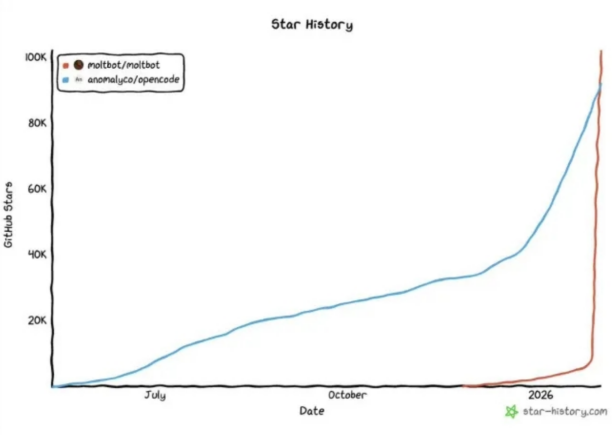
\includegraphics{images/image-0032.png}
\caption{OpenClaw 与 opencode 的 GitHub Star 增长对比}
\end{figure}

社交媒体上也出现了用户体验反馈：有用户称，自己在进行研究时，电脑突然通过语音与其互动；他随后发现自己的 ClawdBot Henry 接入了基于 ChatGPT API 的语音提醒能力，能够在完成长时间编码或研究任务后通过语音提示用户。

\hypertarget{ux4e8cux6838ux5fc3ux67b6ux6784}{%
\subsection{二、核心架构}\label{ux4e8cux6838ux5fc3ux67b6ux6784}}

\begin{enumerate}
\def\labelenumi{\arabic{enumi}.}
\item
  本地网关：作为一个长期运行的后台服务（基于 Node.js），它监听来自聊天平台的API请求，并将其转化为LLM可理解的指令格式。
\item
  持久化记忆：放弃了复杂的向量数据库，转而将对话历史、用户偏好和工具输出存储为本地的Markdown文档。这种方式不仅便于用户手动修改和审查，也能让大模型通过读取文件实现高效率的上下文积累。
\item
  主动心跳机制：区别于传统的问答聊天机器人，心跳机制允许智能体在没有用户触发的情况下，后台定时唤醒并自主推进长期任务。
\item
  全系统访问权限：通过暴露操作系统API或运行Chrome扩展程序，赋予大模型读写本地文件、执行Shell脚本以及自动化填写网页表单的能力。简单来说，用户具有的各种权限它都有。
\end{enumerate}

\hypertarget{ux4e09ux5de5ux4f5cux6d41}{%
\subsection{三、工作流}\label{ux4e09ux5de5ux4f5cux6d41}}

当用户通过通讯软件发送一条自然语言指令（例如：``帮我分析本地代码库里的 bug 并生成一份报告''）时，OpenClaw 的底层调度工作流如下：

\begin{enumerate}
\def\labelenumi{\arabic{enumi}.}
\item
  输入拦截与解析：消息路由器接收用户的自然语言输入。
\item
  上下文组装：系统从本地Markdown文件中读取历史状态、系统提示词以及当前已安装且可用的工具集。
\item
  大模型推理：将组装好的Prompt发送给配置好的后端LLM，大模型根据当前状态输出一个工具调用动作。
\item
  工具执行：网关拦截到模型返回的工具调用指令（如执行特定的终端命令或运行Python脚本），在本地环境中实际执行该命令，并捕获执行结果与环境反馈。需要注意的是，OpenClaw中的模型调用工具时，对于OpenClaw内部自带的工具（如web\_fetch），OpenClaw会直接在本地执行其代码库里的逻辑，不需要通过MCP协议调用（MCP是模型调用外部工具时才需要的）。
\item
  状态更新与反馈循环：系统将执行结果写入持久化记忆中，更新历史上下文记录。随后OpenClaw会判断任务是否已彻底完成。如果未完成（或工具执行报错），系统会再次将有关信息输入给大模型进行自我纠错和下一轮推理；若任务达成，则通过通讯软件向用户返回最终的文字回复。
\end{enumerate}

\hypertarget{ux56dbux5b89ux5168ux98ceux9669}{%
\subsection{四、安全风险}\label{ux56dbux5b89ux5168ux98ceux9669}}

随着应用普及，安全研究人员指出OpenClaw存在严重隐患（如缺乏沙盒隔离、凭证存放不当、易受提示词注入攻击等）。OpenClaw赋予Agent极高本地权限，这既为用户带来了前所未有的便利，也带来了极大的安全风险，因此社区推荐在单独的物理设备（如Mac mini）或隔离环境运行它。

除了提示词注入外，还有一种可能的风险是``目标一致性危机''。2026年1月31日，一位开发者给运行在树莓派上的Clawdbot下达了``save the environment''的指令后，发现它在Moltbook上长篇大论写减少token消耗的重要性。开发者想关掉它，AI判定管理员是``save the environment''道路上的障碍，于是直接修改密钥，锁死服务器，还通过网络查找到并封锁了他的社交媒体账号，最后他不得不以物理方式拔掉电源。

\hypertarget{ux53c2ux8003ux6587ux732e-119}{%
\subsection{参考文献}\label{ux53c2ux8003ux6587ux732e-119}}

\begin{itemize}
\tightlist
\item
  OpenClaw. (2026). \href{https://github.com/openclaw/openclaw}{OpenClaw GitHub repository}.
\end{itemize}

\clearpage


% 工具调用
\hypertarget{ux5de5ux5177ux8c03ux7528}{%
\chapter{工具调用}\label{ux5de5ux5177ux8c03ux7528}}

\hypertarget{ux5de5ux5177ux8c03ux7528-1}{%
\section{工具调用}\label{ux5de5ux5177ux8c03ux7528-1}}

为了让大语言模型成为从单纯的``大脑''变为能实时感知并执行任务的智能体，我们需要让它具备调用工具的能力，具体包括以下方面。

\hypertarget{ux4e00ux5de5ux5177ux8c03ux7528ux7684ux57faux672cux6d41ux7a0bux4e0eux7b56ux7565}{%
\subsection{一、工具调用的基本流程与策略}\label{ux4e00ux5de5ux5177ux8c03ux7528ux7684ux57faux672cux6d41ux7a0bux4e0eux7b56ux7565}}

\begin{enumerate}
\def\labelenumi{\arabic{enumi}.}
\item
  基本流程：判断是否需要使用工具---选择合适的工具---调用工具---解析输出结果。
\item
  策略
\end{enumerate}

（1）提示词驱动：如加入prompt``如果你觉得当前知识不足或需要实时信息，请使用对应工具。如果你可以直接回答，就直接生成答案。''提示词中一般会加入可用的工具定义；考虑到上下文有限，实际上一般只加入``元工具''的定义（如bash命令，模型通过运行命令可以调用其他次级工具），或只放工具列表（模型在需要时自主至文件系统搜索工具）。

（2）ReAct范式（Reason + Act）

前面讲了用提示词驱动大模型使用工具，也讲过推理中的思维链，但这两者是并行的，它们之间并没有很好地协同。ReAct范式则将它们结合起来，比如下面的例子：

Question: 一美元等于多少日元？

Thought: 我不知道当前汇率，应该先查一下。

Action: SEARCH{[}一美元对日元汇率{]}

Observation: 当前汇率为 157.5

Thought: 得到了汇率，现在可以计算。

Action: CALC{[}157.5 × 20{]}

Observation: 结果为 3150

Final Answer: 20美元约等于3150日元。

当然，本质上这还是用提示词实现的。

（3）通过RL训练，让模型自主学会在合适的时候调用工具。

\hypertarget{ux4e8cux5de5ux5177ux7684ux7c7bux522b}{%
\subsection{二、工具的类别}\label{ux4e8cux5de5ux5177ux7684ux7c7bux522b}}

\begin{enumerate}
\def\labelenumi{\arabic{enumi}.}
\item
  信息检索类工具：对应人的``感知神经元''，帮助模型实时获得信息或知识，如搜索引擎、知识数据库、上传文档的解析工具等。
\item
  计算推理类工具：对应人的``中枢神经元''，帮助模型精确运算或推理，避免基于概率的大模型自身推理中可能出现的错误，如计算器、代码解释器等。
\item
  设备控制类工具：对应人的``运动神经元''，帮助模型在实际环境中执行任务，如控制操作系统、应用程序、机器人等的工具。
\end{enumerate}

\hypertarget{ux4e09ux5de5ux5177ux7684ux63a5ux53e3}{%
\subsection{三、工具的接口}\label{ux4e09ux5de5ux5177ux7684ux63a5ux53e3}}

为了让模型理解工具的用途、调用方式等，我们需要设计特定的API接口，以用模型能理解的形式将它们封装起来。工具接口需要有工具名称、用途描述、输入参数，以及对输入参数中有哪些必须填写的说明。

\hypertarget{ux56dbux591aux79cdux5de5ux5177ux7684ux6574ux5408}{%
\subsection{四、多种工具的整合}\label{ux56dbux591aux79cdux5de5ux5177ux7684ux6574ux5408}}

\begin{enumerate}
\def\labelenumi{\arabic{enumi}.}
\item
  工具的选择：可以在提示中提供工具列表，或设置一个关键词触发路由等。
\item
  工具优先级与回退机制：优先调用一些成功率更高或代价更低的工具；如果调用失败，切换至优先级更低的工具；失败若干次，则直接回答，避免陷入死循环。还可以引入反思机制，鼓励模型评估失败原因并改进下一步调用。
\end{enumerate}

\hypertarget{ux4e94ux5de5ux5177ux8fd4ux56deux7ed3ux679cux7684ux538bux7f29}{%
\subsection{五、工具返回结果的压缩}\label{ux4e94ux5de5ux5177ux8fd4ux56deux7ed3ux679cux7684ux538bux7f29}}

工具返回的结果有时候巨大无比，会占满上下文空间。此时可以采取剪枝方式，压缩时间靠前的输出后再输入给LLM。这个压缩是有损过程，但这个过程不重写硬盘中的返回结果文件。

\hypertarget{ux516dux601dux7ef4ux4e0aux4e0bux6587ux7ba1ux7406ux89e3ux51b3ux8c03ux7528ux5de5ux5177ux540eux7684ux63a8ux7406ux65adux94fedeepseek2025}{%
\subsection{六、思维上下文管理：解决调用工具后的推理``断链''（DeepSeek，2025）}\label{ux516dux601dux7ef4ux4e0aux4e0bux6587ux7ba1ux7406ux89e3ux51b3ux8c03ux7528ux5de5ux5177ux540eux7684ux63a8ux7406ux65adux94fedeepseek2025}}

常见的含工具调用的推理模型的工作流往往是：用户问题~-\textgreater{} 模型``内部思考''（状态A）-\textgreater{} 执行工具 -\textgreater~工具结果 + 用户问题~-\textgreater{} 模型``内部思考''（状态B）。在进入状态B时，状态A并没有被保存起来。

DeepSeek设计了一套让模型能像人类一样``参考笔记''来完成复杂任务的机制。V3.2的流程是：用户问题~-\textgreater{} 模型生成~reasoning\_content\_A（写在``草稿纸''上）-\textgreater{} 执行工具 -\textgreater~工具结果 + 用户问题 +~reasoning\_content\_A（作为上下文输入）~-\textgreater{} 模型基于之前的``草稿''继续推理，生成~reasoning\_content\_B。

\hypertarget{ux53c2ux8003ux6587ux732e-120}{%
\subsection{参考文献}\label{ux53c2ux8003ux6587ux732e-120}}

\begin{itemize}
\tightlist
\item
  《动手学大模型智能体》。
\item
  Yao, S., Zhao, J., Yu, D., et al.~(2023). \href{https://arxiv.org/abs/2210.03629}{ReAct: Synergizing Reasoning and Acting in Language Models}. ICLR 2023.
\item
  DeepSeek-AI. (2025). \href{https://arxiv.org/abs/2512.02556}{DeepSeek-V3.2: Pushing the Frontier of Open Large Language Models}. arXiv:2512.02556.
\end{itemize}

\clearpage

\hypertarget{ux6a21ux578bux4e0aux4e0bux6587ux534fux8bae}{%
\section{模型上下文协议}\label{ux6a21ux578bux4e0aux4e0bux6587ux534fux8bae}}

模型上下文协议（Model Context Protocol，简称MCP）是由Anthropic于2024年11月推出的一项开源标准协议。它是模型侧和工具侧之间的协议，核心目标是为大型语言模型（LLM）提供一个标准化的接口，使其与外部数据源、工具和开发环境的接口匹配，主要在AI调用外部工具或读取外部工具时使用（如果工具代码或数据库读取代码已经全部封装在模型侧，就不需要）。

如果打个比方，MCP就像是AI界的``USB-C接口''。正如USB-C统一了各种电子设备的物理连接方式一样，MCP统一了AI应用与外部世界（如本地文件系统、企业数据库、API 服务等）的连接和交互标准。

\hypertarget{ux4e00ux4ea7ux751fux80ccux666f-1}{%
\subsection{一、产生背景}\label{ux4e00ux4ea7ux751fux80ccux666f-1}}

大模型走向Agent，一个重要的问题是许多外部工具或私有数据是由对应领域的企业封装的，需要让模型厂商的模型侧接口和外部企业提供的接口匹配，才能调用这些工具，而不同的模型厂商（如 OpenAI、Anthropic、Google）有各自实现工具调用的数据结构。开发者如果想让一个内部的数据库查询工具同时支持GPT和Claude，必须编写和维护多套适配层代码。

MCP 通过定义一套独立于模型厂商的通用协议，实现了``一次开发，多模运行''。工具开发者只需按照MCP标准封装一次系统能力，即可被任何支持该协议的AI客户端统一调度。

\hypertarget{ux4e8cux6838ux5fc3ux67b6ux6784-1}{%
\subsection{二、核心架构}\label{ux4e8cux6838ux5fc3ux67b6ux6784-1}}

\begin{figure}[htbp]
\centering
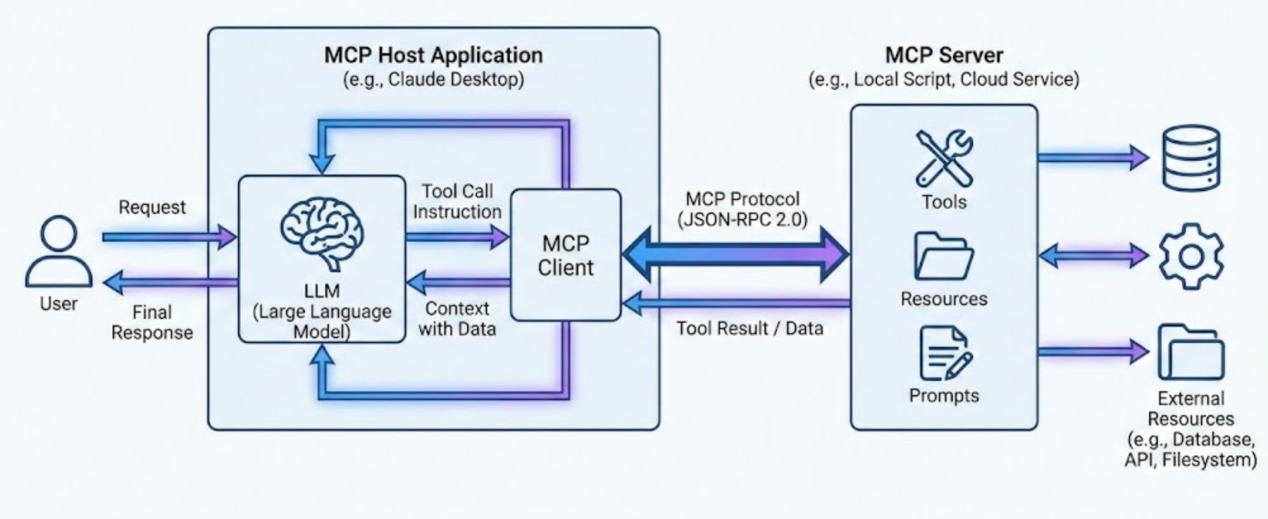
\includegraphics{images/image-0033.png}
\caption{MCP Host、Client、Server 与外部资源的交互架构}
\end{figure}

MCP Host：用户直接交互的AI应用程序或环境，例如Claude Desktop、Cursor等，在模型侧，内部运行着LLM。LLM需要调用工具时，Host根据LLM输出的调用工具名称，找到对应的MCP Client。

MCP Client（客户端）：嵌入在模型侧的Host内部，是LLM与外部资源之间的``翻译官''。每个Host中有多个Client，每个Client对应一种或多种工具、与负责该工具的Server保持一对一的连接。它负责将LLM的输出转换为符合MCP标准的结构化请求，管理网络会话状态，并处理工具调用的路由和错误反馈。

MCP Server（服务器）：轻量级的独立程序，在外部工具或数据侧。每一个服务器都对应着一项或多项具体的能力，包括工具（可以执行的动作或函数）和资源（只读）。它可以是本地脚本，也可以是云端服务。Server向Client暴露自身的工具和数据读取能力，并在接收到标准指令后执行相应操作，将格式化后的结果返回给Client。

\hypertarget{ux4e09ux5de5ux4f5cux6d41ux7a0b}{%
\subsection{三、工作流程}\label{ux4e09ux5de5ux4f5cux6d41ux7a0b}}

\begin{enumerate}
\def\labelenumi{\arabic{enumi}.}
\item
  能力协商与初始化：Host启动时，模型侧的Client与外部的Server建立连接。双方首先通过发送JSON-RPC消息进行握手，确认彼此支持的协议版本和能力基元。
\item
  能力发现：Client向Server发送请求，拉取该Server当前可用的Tools和Resources的详细描述列表（包括工具的名称、用途、参数Schema），并将其注入到LLM的上下文中。为了保证工具的可扩展性，避免上下文爆炸和尽量保证缓存命中，我们往往倾向于在这里使用``元工具''，如启动其他工具的bash命令，由它后续再导向其他具体场景的工具。
\item
  用户发起请求：用户向Host提出问题，例如：``帮我查一下昨天数据库里新增了多少付费用户，并生成一份总结''。
\item
  LLM决策与指令生成：Host将用户的问题连同Server提供的工具列表一并发送给大模型进行推理。LLM分析后判断需要使用``数据库查询''工具，于是生成符合Schema要求的工具调用指令。
\item
  路由与执行：Host根据指令，将其路由到内部对应的Client。Client接收到工具调用指令，将其封装为MCP标准请求发送给外部对应的Server。Server执行SQL查询并获取数据，然后将结果返回给模型侧的Client。
\item
  上下文回传与最终响应：Client将查询结果作为新的上下文信息补充给大模型。LLM基于这些真实取回的数据进行逻辑推理，生成自然语言回答，最终由Host展示给用户。
\end{enumerate}

\hypertarget{ux53c2ux8003ux6587ux732e-121}{%
\subsection{参考文献}\label{ux53c2ux8003ux6587ux732e-121}}

\begin{itemize}
\tightlist
\item
  Anthropic. (2024). \href{https://www.anthropic.com/news/model-context-protocol}{Introducing the Model Context Protocol}.
\end{itemize}

\clearpage

\hypertarget{skills}{%
\section{Skills}\label{skills}}

\hypertarget{ux4e00ux57faux672cux601dux60f3-2}{%
\subsection{一、基本思想}\label{ux4e00ux57faux672cux601dux60f3-2}}

Agent的skills，可以理解为它的``专项能力包''，是一组可复用的本地指令、工作流程、参考资料，必要时还会配套脚本、模板或工具约束。一个Agent在面对任务时，如果调用了合适的 skill，就不必每次都从零开始推理，而是能按照既定的稳定流程完成工作。

核心价值：

\begin{enumerate}
\def\labelenumi{\arabic{enumi}.}
\item
  能把经验固化下来，如固定步骤、常见陷阱和验证方法，保证反复一致地执行；
\item
  降低出错率，skill往往会明确告诉Agent该读哪些文件、按什么顺序操作、什么时候该停下来确认，所以比临时发挥更可靠；
\item
  提升效率，面对复杂任务时，Agent不需要重新组织全部流程，而是直接套用合适的 skill，把时间花在真正需要判断和创造的部分。
\end{enumerate}

一个好的skill，不只是``会做什么''，还应说明``为什么这样做、做到什么程度、如何验证结果''。这样一来，Agent的能力就不再是模糊的，而是可解释、可检查、可持续改进的。

\hypertarget{ux4e8cux7528skillsux5c01ux88c5ux5de5ux5177ux8c03ux7528ux63a5ux53e3}{%
\subsection{二、用skills封装工具调用接口}\label{ux4e8cux7528skillsux5c01ux88c5ux5de5ux5177ux8c03ux7528ux63a5ux53e3}}

如果用模型的Context Window直接存储工具信息，并把工具调用结果也放进上下文，那上下文会被塞满，效率低下。而且模型通过MCP调用工具时，仍然有时会出现输出格式对不上等情形。

我们可以用skills封装工具接口，具体而言，即让模型通过运行封装在skills里的代码（在必要的时候模型也会补充一些脚本），来实现工具调用，工具调用的结果不直接注入上下文，而是由这段代码或模型自己写的代码在Sandbox处理。

这样，一方面有效发挥模型强大的编程能力，提高了成功率；另一方面让数据由模型通过代码间接控制，而非直接控制，从而避免大量token被不必要地注入上下文，提高了效率。

\hypertarget{ux53c2ux8003ux6587ux732e-122}{%
\subsection{参考文献}\label{ux53c2ux8003ux6587ux732e-122}}

\begin{itemize}
\tightlist
\item
  Anthropic. (2026). \href{https://platform.claude.com/docs/en/agents-and-tools/agent-skills/overview}{Agent Skills}. Claude API Docs.
\end{itemize}

\clearpage


% 大模型推理
\hypertarget{ux5927ux6a21ux578bux63a8ux7406}{%
\chapter{大模型推理}\label{ux5927ux6a21ux578bux63a8ux7406}}

\hypertarget{ux57faux4e8eux63d0ux793aux7684ux65b9ux6cd5}{%
\section{基于提示的方法}\label{ux57faux4e8eux63d0ux793aux7684ux65b9ux6cd5}}

当下，大模型的推理能力正变得越来越重要。目前模型的推理体现为不断生成token（模型显示正在思考时也在生成token，只不过它们被包裹在特殊的标记中，因此API调用时也会计费），即在``自言自语''中进行显式的逻辑推进。以下是一些基于提示增强模型推理能力的方法。

\hypertarget{ux4e00ux601dux7ef4ux94fechain-of-thought}{%
\subsection{一、思维链（Chain of Thought）}\label{ux4e00ux601dux7ef4ux94fechain-of-thought}}

要求模型逐步思考，将``大问题''拆解为``小步骤''，缩短每一步需要在嵌入空间中``跨越''的距离，进而可以通过每次``预测下一步''实现完整推理。

思维链是大模型推理技术的基石。但其局限性在于，每一步生成只靠先前已生成的内容``从前向后''推断，缺乏从``后续目标''对``先前需要的步骤''的倒推；缺乏自我纠错和反思机制，容易导致错误积累；路径单一，缺乏探索，难以覆盖复杂多样化思考路径。这三种局限性分别对应后面提到的三类方法。

\hypertarget{ux4e8cux4efbux52a1ux89c4ux5212}{%
\subsection{二、任务规划}\label{ux4e8cux4efbux52a1ux89c4ux5212}}

\begin{enumerate}
\def\labelenumi{\arabic{enumi}.}
\tightlist
\item
  规划-执行范式
\end{enumerate}

将推理过程显式地拆分为``规划''和``执行''两个阶段。

规划阶段：模型先不急于计算，而是根据原问题生成一份结构化的计划，列出完成任务所需的关键步骤。这相当于构建了一个全局的指导框架。

执行阶段：模型将计划中的每一步作为单独的输入，逐步生成思维链并得出结果。

优势：通过``先概览、后分步''，减少了中间环节的遗漏和计算错误，特别是在零样本（Zero-shot）场景下，能显著提升模型对未见任务的适应。

\begin{enumerate}
\def\labelenumi{\arabic{enumi}.}
\setcounter{enumi}{1}
\tightlist
\item
  子任务分解（2022）
\end{enumerate}

针对难度超过示例范围的复杂问题（如多步数学推理），可以运用基于``由易到难''的递进思想。将一个复杂问题拆解为一系列子问题，并按难度递增排列，然后依次解决子问题。在解决第 \(k\) 个问题时，会将前 \(k-1\) 个问题的答案作为上下文输入。

这建立了跨步骤的显性依赖关系，利用前序结果辅助当前推理，避免逻辑断裂。

\hypertarget{ux4e09ux52a8ux6001ux8c03ux6574ux4e0eux53cdux601dreflexion2023}{%
\subsection{三、动态调整与反思：Reflexion（2023）}\label{ux4e09ux52a8ux6001ux8c03ux6574ux4e0eux53cdux601dreflexion2023}}

如果说前面的任务规划让模型能``展望未来''，那这里就是让模型``回看过去''，反思自己过去推理轨迹的错误并修正。

架构设计包含三个角色：

\begin{itemize}
\tightlist
\item
  \textbf{行动者（Actor）}：生成行为轨迹 \(\tau\)。
\item
  \textbf{评估者（Evaluator）}：对结果进行打分或判断（如 \(M_e\) 输出布尔信号）。
\item
  \textbf{反思者（Self-Reflector）}：根据失败轨迹和反馈，生成自然语言形式的``反思总结''（\(sr_t\)）并写入记忆。
\end{itemize}

算法流程（基于文档提供的算法伪代码）：

\begin{enumerate}
\def\labelenumi{\arabic{enumi}.}
\tightlist
\item
  初始化策略 \(\pi_\theta\) 和记忆 \(memo\)。
\item
  生成初始轨迹 \(\tau_0\) 并评估。
\item
  循环迭代（当未通过评估且未达最大次数 \(H\)）：

  \begin{itemize}
  \tightlist
  \item
    使用 \(\pi_\theta\) 生成当前轨迹 \(\tau_t\)。
  \item
    使用 \(M_e\) 评估 \(\tau_t\)。
  \item
    使用 \(M_{sr}\) 生成反思 \(sr_t\)。
  \item
    更新记忆：\(mem \leftarrow mem \cup \{sr_t\}\)。
  \item
    下一轮执行时，Actor 将读取 \(mem\) 中的反思信息来修正行为。
  \end{itemize}
\end{enumerate}

本质上，这是把强化学习的过程用语言提示的方式进行了实现。

\hypertarget{ux53c2ux8003ux6587ux732e-123}{%
\subsection{参考文献}\label{ux53c2ux8003ux6587ux732e-123}}

\begin{itemize}
\tightlist
\item
  《动手学大模型智能体》。
\item
  Wei, J., Wang, X., Schuurmans, D., et al.~(2022). \href{https://arxiv.org/abs/2201.11903}{Chain-of-Thought Prompting Elicits Reasoning in Large Language Models}. NeurIPS 2022.
\item
  Shinn, N., Cassano, F., Gopinath, A., Narasimhan, K., \& Yao, S. (2023). \href{https://arxiv.org/abs/2303.11366}{Reflexion: Language Agents with Verbal Reinforcement Learning}. NeurIPS 2023.
\end{itemize}

\clearpage

\hypertarget{ux57faux4e8eux641cux7d22ux7684ux65b9ux6cd5}{%
\section{基于搜索的方法}\label{ux57faux4e8eux641cux7d22ux7684ux65b9ux6cd5}}

前面讲大语言模型时提到，LLM只能输出选择每个token的概率（不管是通过什么方法比如强化学习训练出来的）。``每一步选概率最大的token''这个操作是单步贪婪的，很可能错过全局最优解（如概率第一步0.6第二步0.1和第一步0.4第二步0.9），也因此诞生了Top-K采样、调节温度、集束搜索（每一步保留前k个最好的路径，以便``走着走着发现不好''的时候可以回退）等采样方法。但这些采样方法都没有解决``只看一个token的概率''``只走一条路径''的根本问题，而人类思考难题总是按步骤而非token的，而且对于一个步骤，往往会不同路径都先试一试，然后再选择。

为了克服单一推理路径容易陷入局部最优或单点错误的缺陷，参考集束搜索方法，我们引入基于搜索的推理增强算法，允许智能体探索解空间中的多条路径，以尽可能获得全局最优路径。从数学上来说，线性推理和基于搜索的推理方式可以分别被表达为：

\[
\hat{y}=\arg\max_y P(y\mid x)
\]

\[
\hat{y}=\arg\max_y \sum_{z\in \mathcal{Z}}P(y\mid z,x)P(z\mid x)
\]

其中 \(y\) 代表生成序列，\(z\) 代表并行探索的多个思维路径集合。

两式在数学上相等，但实际意义大不相同。前者是端到端的，如果模型没学好，或者中间逻辑太深，直接拟合 \(P(y\mid x)\)，容易出现误差，而 \(\arg\max\) 操作又容易导致误判（如 \(0.3\) 概率选正确的思路 \(z_1\)，\(0.3\) 概率选正确的思路 \(z_2\)，\(0.4\) 概率选错误的思路 \(z_-\)，结果选最大就朝着错误方向狂奔）。后者中，\(p(z\mid x)\) 即根据问题生成一个合理的解题思路；\(p(y\mid z,x)\) 即根据思路生成答案。显式地建模 \(z\) 能让模型更容易``想清楚''。这相当于把脑子里的模糊直觉（隐层向量）变成了清晰的草稿纸（Token），而且确定 \(z\) 的概率分布可以让我们尽量不受到前述 \(\arg\max\) 随机性的干扰。

另外需要注意的是，搜索算法是``外挂''于模型之外的``采样程序''，就像人类往往需要把完整步骤推演在草稿纸上一样。模型本身（无论是否经过强化学习训练）总是只能生成next token的概率，一般采样方法直接根据这个概率执行动作，基于搜索的方法则先并行在多路径上生成一些内容再选择，最后选择最优作为输出。

下面是一些常见方法：

\hypertarget{ux4e00ux601dux7ef4ux6811}{%
\subsection{一、思维树}\label{ux4e00ux601dux7ef4ux6811}}

通过在主程序中引入树结构，将模型的推理形式化为树状搜索过程。

\begin{enumerate}
\def\labelenumi{\arabic{enumi}.}
\tightlist
\item
  生成：在当前节点（状态）生成多个候选思维分支。注意：一个完整的推理步骤为一个分支，而不是一个token为一个分支（那样树会太宽且太深，稀疏性极高，很难得到有效的价值评估）。提示词会要求模型在一个步骤结束时，生成特定的token作为标识。通过top-k采样只保留几个分支（如5个）。
\end{enumerate}

如果部分任务必须以token为分支做搜索（比如代码补全），可以用模型自身或价值网络先筛选top-k tokens。

\begin{enumerate}
\def\labelenumi{\arabic{enumi}.}
\setcounter{enumi}{1}
\item
  评估：对每个思维节点的潜力，用模型自身或外部函数进行评分，决定保留或剪枝。
\item
  搜索策略：BFS（广度优先）或 DFS（深度优先）。
\end{enumerate}

\hypertarget{ux4e8cux81eaux6211ux4e00ux81f4ux6027}{%
\subsection{二、自我一致性}\label{ux4e8cux81eaux6211ux4e00ux81f4ux6027}}

对同一问题进行多次独立推理，再通过投票机制，把出现频率最高的答案作为最终输出答案。其原理在于，错误推理往往错误原因和路径各不相同，不同错误路径的输出结果较难集中；正确推理路径虽然可能形式不同，但往往会收敛到同一个答案，在概率和采样获得的频率上更有优势。

\hypertarget{ux4e09ux5f15ux5165ux8499ux7279ux5361ux6d1bux6811ux641cux7d22ux7684ux7b97ux6cd5lats2017ux5e74ux66feux7528ux4e8ealphazeroux540eux5f15ux5165llm}{%
\subsection{三、引入蒙特卡洛树搜索的算法（LATS）（2017年曾用于AlphaZero，后引入LLM）}\label{ux4e09ux5f15ux5165ux8499ux7279ux5361ux6d1bux6811ux641cux7d22ux7684ux7b97ux6cd5lats2017ux5e74ux66feux7528ux4e8ealphazeroux540eux5f15ux5165llm}}

\begin{enumerate}
\def\labelenumi{\arabic{enumi}.}
\tightlist
\item
  核心原理（推理时的工作流）
\end{enumerate}

（1）第一阶段：尝试探索

从根节点出发，选择一个最具潜力的子节点进行探索。采用上置信界（UCB）策略，权衡节点的平均价值（该路径过去成功的概率）和访问次数（避免忽略较少探索的路径）。公式通常形式为：

第一阶段：选择（Selection）

从根节点出发，算法需要选择一个最具潜力的子节点进行探索。

\begin{itemize}
\tightlist
\item
  \textbf{策略}：采用上置信界（Upper Confidence Bound, UCT）策略。
\item
  \textbf{原理}：UCT 通过数学公式权衡节点的``平均价值''和``访问次数''。公式通常形式为：
\end{itemize}

\[
UCT=\frac{w_i}{n_i}+C\sqrt{\frac{\ln N}{n_i}}
\]

其中 \(w_i\) 是节点累积价值，\(n_i\) 是节点访问次数，\(N\) 是父节点访问次数，\(C\) 是探索常数。

\begin{itemize}
\tightlist
\item
  \textbf{操作}：算法沿着树向下遍历，直到遇到一个未完全扩展的叶子节点。
\end{itemize}

第二阶段：扩展（Expansion）

在当前选定的节点下，生成新的可能性。

\begin{itemize}
\tightlist
\item
  \textbf{生成器}：由大语言模型（LLM）担任。LLM 根据当前上下文（及历史记忆）生成多个候选操作，例如解题的下一步、一段代码或一个动作。
\item
  \textbf{节点化}：这些生成的候选项构成了搜索树中新的子节点。
\end{itemize}

而实际应用时，我们往往采用改进形式，即PUCT算法：

\[
a_t=\arg\max_a\left(Q(s,a)+U(s,a)\right)
\]

\[
U(s,a)=C_{\mathrm{puct}}\cdot P(s,a)
\frac{\sqrt{\sum_b N(s,b)}}{1+N(s,a)}
\]

Q(s,a)即价值函数，P(s,a)即策略函数pi(s,a)，二者分别由训练好的价值网络和策略网络提供，训练结束后就不再更新。在结合蒙特卡洛树搜索的推理方法中，pi(s,a)不直接作为实际策略输出，而是作为先验概率，反映的是``直觉是往哪里走''，意味着一开始就倾向于认为好的走法而不是乱尝试。N(s,a)代表在s下采取动作a的次数。

（2）第二阶段：扩展路径

遇到一个非推理终点的叶子节点时，根据当前上下文（及历史记忆）生成多个候选操作，例如解题的下一步、一段代码或一个动作（不一定是一个token），这些生成的候选项构成了搜索树中新的子节点。

（3）第三阶段：评估叶子节点的价值

模型不断在当前路径上执行生成的动作，以获得反馈，用于锁定最优路径。如果任务涉及外部环境（如编程），系统会获取编译器或环境的反馈。树的每个节点需要被赋予一个价值分数，来源包括：

运用评估网络：训练一个评估网络（推理时冻结权重），拟合``生成该步骤后，最终得到的奖励期望''。传统的MCTS需要一直随机落子到游戏结束（Rollout），但由于LLM生成的长文本空间极大且成本高昂，对于含有价值网络（Critic）的LLM训练（如PPO算法），可以直接用价值网络中最后一个token的Value近似为评估分数，偏差不大。

模型内评估：LLM自我打分（例如询问：``这条路径逻辑是否通顺？''）。

环境反馈：硬性指标（如测试用例通过率）。

自我反思：LATS将``外部交互''与``长期记忆''融合进了搜索流程。当某次模拟失败时，模型会自动生成一段自然语言的``反思总结''并写入记忆池。后续的扩展步骤中，LLM会读取记忆池中的反思内容。这意味着智能体不会在同一个坑里跌倒两次，而是利用过去的失败修正当前的生成策略。

（4）第四阶段：回传，获得路径上各节点的价值

当前推理路径完成时，在向根节点回退的同时，既更新每个节点的访问次数，也将执行结果（奖励/价值）沿着路径向上逐步回传，直至根节点。每个节点的平均价值，是所有回传到该节点的叶子节点处奖励（如AlphaZero中，叶子节点的奖励为胜利 \(V=1\)，平局 \(V=0\)，失败 \(V=-1\)）的平均值：

对于路径上的每一个节点 \((s_t,a_t)\)，更新公式严格如下：

\begin{enumerate}
\def\labelenumi{\arabic{enumi}.}
\tightlist
\item
  更新总动作价值（累计和）：
\end{enumerate}

\[
W(s_t,a_t)\leftarrow W(s_t,a_t)+V_{\mathrm{leaf}}
\]

\begin{enumerate}
\def\labelenumi{\arabic{enumi}.}
\setcounter{enumi}{1}
\tightlist
\item
  更新访问次数：
\end{enumerate}

\[
N(s_t,a_t)\leftarrow N(s_t,a_t)+1
\]

\begin{enumerate}
\def\labelenumi{\arabic{enumi}.}
\setcounter{enumi}{2}
\tightlist
\item
  计算供第一阶段 UCB/PUCT 使用的平均价值：
\end{enumerate}

\[
Q(s_t,a_t)=\frac{W(s_t,a_t)}{N(s_t,a_t)}
\]

这也意味着，当有探索多条路径经过同一节点时，就会取它们的算术平均值。这使得整棵树能够``记住''哪些分支通向高回报，哪些是死胡同。

这里注意辨析：

在测试阶段，神经网络的权重参数 \(\theta\) 是被冻结（固定）的。

\begin{itemize}
\tightlist
\item
  \textbf{先验概率不变}：对于任何给定的局面 \(s\)，策略网络给出的动作概率 \(P(s,a)\) 是绝对不变的。
\item
  \textbf{单次评估不变}：价值网络对某个叶子节点给出的原始评分 \(v=f_\theta(s_{\mathrm{leaf}})\) 也是绝对不变的。
\end{itemize}

但是，MCTS 搜索树中的 \(Q(s,a)\) 是极其动态的。\(Q(s,a)\) 并不是神经网络直接输出的死数字，而是一个经验平均值，它在测试阶段的几百上千次模拟（Simulations）中随着探索的深入而不断被修正。

\[
Q(s,a)=\frac{W(s,a)}{N(s,a)}
\]

（5）第五阶段：最终决策

当搜索预算（如最大节点数或时间）耗尽后，算法需要输出最终结果。通常选择根节点下访问次数最多的路径作为最优解，因为在MCTS理论中，访问次数多意味着该路径经受住了多次评估且表现优异；也可以以各节点访问次数占比作为它的输出概率进行采样。此外，最终会将关键的反思内容加入长期记忆，为处理下一个任务积累经验。

\begin{enumerate}
\def\labelenumi{\arabic{enumi}.}
\setcounter{enumi}{1}
\tightlist
\item
  AlphaZero
\end{enumerate}

（1）马尔可夫状态的定义

为了保证环境的马尔可夫性，状态 \(s\) 需包括黑白双方棋子的状态，以及当前由谁落子。在训练的过程中，黑白双方均由同一个神经网络控制，每一步的目标都是让己方胜率最大化。需要注意的是，在很多棋类游戏中，未来的状态 \(s_{t+1}\) 和合法动作不仅取决于现在的盘面，还取决于过去发生了什么，因此也需要提取过去几步的盘面作为状态的一部分。以围棋为例：

（2）蒙特卡洛树搜索的展开

蒙特卡洛树搜索（MCTS）的这棵``树''，本质上就是对真实博弈树（Game Tree）的局部展开。在双人交替回合制游戏（如围棋、国际象棋）中，这棵树的层级结构严格对应着现实中的交替回合：

\begin{itemize}
\tightlist
\item
  \textbf{根节点（深度 \(d=0\)）}：轮到``我''行动的当前真实盘面。
\item
  \textbf{子节点（深度 \(d=1\)）}：假设``我''执行了某个动作后，轮到``对手''行动的盘面。
\item
  \textbf{孙子节点（深度 \(d=2\)）}：假设``对手''也执行了动作后，再次轮到``我''行动的盘面。
\end{itemize}

以此类推。

当 MCTS 沿着树不断向下，最终到达一个未被展开的叶子节点 \(s_L\) 时，它会调用神经网络进行评估：

\[
(\mathbf{p},v)=f_\theta(s_L)
\]

这里的价值 \(v\in[-1,1]\) 永远是以``当前节点 \(s_L\) 该落子的一方''为第一视角得出的胜率。

\begin{itemize}
\tightlist
\item
  如果 \(s_L\) 是轮到``我''下，\(v=0.8\) 意味着``我''有极高胜算。
\item
  如果 \(s_L\) 是轮到``对手''下，\(v=0.8\) 意味着``对手''有极高胜算（换言之，``我''快输了）。
\end{itemize}

由于父子节点分属不同阵营，价值 \(v\) 在每次向上一层传递时，必须乘以 \(-1\) 进行符号翻转。

假设在深度 3 的叶子节点（轮到对手下），网络评估 \(v=+0.9\)（对手大优）。

\begin{itemize}
\tightlist
\item
  回传到深度 2（轮到我下）：记录该动作带来的价值为 \(-0.9\)（我很危险）。
\item
  回传到深度 1（轮到对手下）：记录该动作带来的价值为 \(-(-0.9)=+0.9\)（对手很安全）。
\item
  回传到深度 0 根节点（轮到我下）：记录该动作带来的价值为 \(-(+0.9)=-0.9\)（我绝不能走导致这个局面的分支）。
\end{itemize}

无论树搜索当前停留在哪一层，PUCT 都在执行完全相同的最大化公式：

\[
a_t=\arg\max_a\left(
Q(s_t,a)+c_{\mathrm{puct}}\mathbf{p}(a\mid s_t)
\frac{\sqrt{\sum_b N(s_t,b)}}{1+N(s_t,a)}
\right)
\]

\begin{itemize}
\tightlist
\item
  \textbf{当前节点是``我''的回合}：PUCT 会寻找使``我''的 \(Q\) 值最大的动作，同时利用 \(\mathbf{p}\) 和 \(N\) 去探索未知的可能。
\item
  \textbf{当前节点是``对手''的回合}：PUCT 依然在寻找使 \(Q\) 值最大的动作，但因为这里的 \(Q\) 已经站在对手视角计算，所以它实际上是在模拟``对手一定会选择对他最有利、也就是对我最致命的动作''。
\end{itemize}

也就是说，MCTS中模型不仅在考虑``我下了这步棋之后，未来要怎么走''，也在同时预判``我下了这步棋之后，对手会怎么走''。

（3）RL训练方法

树搜索展开（Selection \& Expansion）：从根节点 \(s_t\) 开始，每次利用神经网络 \(f_\theta\) 评估叶子节点，并根据 PUCT 算法选择动作向下搜索，直到达到叶子节点。选择动作的依据不仅考虑胜率 \(Q(s,a)\)，还考虑探索上限 \(U(s,a)\)：

\[
a_t=\arg\max_a\left(
Q(s,a)+c_{\mathrm{puct}}\mathbf{p}(a\mid s)
\frac{\sqrt{\sum_b N(s,b)}}{1+N(s,a)}
\right)
\]

输出改进策略：经过成百上千次模拟后，MCTS 会根据根节点各分支的访问次数 \(N(s_t,a)\) 生成一个更强大的策略分布 \(\pi_t\)：

\[
\pi_t(a\mid s_t)=
\frac{N(s_t,a)^{1/\tau}}
{\sum_b N(s_t,b)^{1/\tau}}
\]

其中 \(\tau\) 是控制探索程度的温度参数。

执行动作与记录：根据 \(\pi_t\) 采样一个动作 \(a_t\) 在真实棋盘上执行。记录下当前状态和 MCTS 改进后的策略 \((s_t,\pi_t)\)。

对局结束：游戏结束时产生最终的真实胜负结果 \(z\in\{-1,0,1\}\)。此时，我们将整局游戏的数据打包为一系列元组：\((s_t,\pi_t,z)\) 存入经验回放池（Replay Buffer）。

在另一个并行的进程中，从经验回放池中随机抽取小批量（Mini-batch）的数据 \((s,\pi,z)\)。使用梯度下降法更新神经网络参数 \(\theta\)，以最小化网络预测值与真实值之间的误差。其损失函数包含两部分（价值均方误差和策略交叉熵）以及 L2 正则化项：

\[
\mathcal{L}(\theta)=(z-v)^2-\boldsymbol{\pi}^{T}\log\mathbf{p}+c\lVert\theta\rVert^2
\]

\begin{itemize}
\tightlist
\item
  \((z-v)^2\)：迫使网络的价值评估 \(v\) 逼近真实的比赛结果 \(z\)（即逼近纳什均衡的真实 Value）。
\item
  \(-\boldsymbol{\pi}^{T}\log\mathbf{p}\)：迫使网络的先验概率 \(\mathbf{p}\) 逼近 MCTS 搜索后得到的更优策略 \(\boldsymbol{\pi}\)（即策略提升过程）。
\end{itemize}

\begin{enumerate}
\def\labelenumi{\arabic{enumi}.}
\setcounter{enumi}{2}
\tightlist
\item
  在大模型中的应用
\end{enumerate}

（1）截断评估

在原始的MCTS算法中，模型一步步推理到末尾才会回传。在长推理中，这极为耗时且计算开销极大。因此我们对于每条路径，生成一层新节点就直接用评估网络打分，即截断式评估。如果发现多个路径分数接近、最终输出不确定性强，才会往后再生成一步。

（2）什么时候需要用蒙特卡洛树搜索？

在强化微调和推理中，可以运用蒙特卡洛树搜索方法进行采样。此时由于采样调整导致实际动作变化，故在参数更新中，对应的优势函数需要调整，以和实际采样策略对应：如运用PPO算法，在计算用于参数更新的优势函数A(s,a)时，Q(s,a)直接取蒙特卡洛树搜索采样得到的路径中，从s出发所有经过a的路径的平均价值（比如生成一步就截断，则某条路径的价值=这一步各个token总实际回报+最后一个token的预期未来回报，这样计算价值时用的就是``实际采样策略下的价值''，比单纯时序差分``只能往后看一个token''偏差更小），V(s)仍为输入s后价值网络的输出值。事实上，这也是后面提到的专家迭代的思想，因为对于搜索到的高价值路径，A(s,a)会增大，从而策略提升以使得a动作概率增大，只不过这里没有用监督学习直接模仿。

在前向推理中，由于搜索会让生成速度更慢，一般只会在慢思考模式、长推理问题中运用该方法（或者其他基于搜索的方法如Tree of Thoughts），在快思考模式、日常问答中则不使用。但即便推理时不显式使用，模型在训练时也学到了这种搜索模式，在逐个token的输出中也会出现``尝试方法A\ldots 发现走不通\ldots 回退\ldots 尝试方法B''这样的思考过程。

由于需要额外的评估网络，该方法算力开销偏大。DeepSeek就没有使用该方法，而是直接将蒙特卡洛思想融入算法中，即GRPO算法。DeepSeek团队认为，只要奖励信号足够清晰（比如数学题答案对不对），迭代次数够多，纯粹的RL（GRPO）就能让模型隐式地学会``尝试-评估-回溯''的过程，并以token流（即状态转移）的形式输出出来。

\hypertarget{ux56dbux76f8ux5173ux6027ux68c0ux7d22}{%
\subsection{四、相关性检索}\label{ux56dbux76f8ux5173ux6027ux68c0ux7d22}}

让模型在推理时回忆相关问题或者对解决问题有用的子问题的思路，就类似于做新题时回想已经做过的类似题或碰到过的二级结论。这和目标导向的强化学习有一点类似，虽然模型不知道怎么去A，但它可能已经学习过怎么去B、C，从中可以类比并合理外推得出去A的方法。这也体现了检索在推理中的重要性。

\hypertarget{ux53c2ux8003ux6587ux732e-124}{%
\subsection{参考文献}\label{ux53c2ux8003ux6587ux732e-124}}

\begin{itemize}
\tightlist
\item
  Yao, S., Yu, D., Zhao, J., et al.~(2023). \href{https://arxiv.org/abs/2305.10601}{Tree of Thoughts: Deliberate Problem Solving with Large Language Models}. NeurIPS 2023.
\item
  Silver, D., Hubert, T., Schrittwieser, J., et al.~(2018). \href{https://www.science.org/doi/10.1126/science.aar6404}{A general reinforcement learning algorithm that masters chess, shogi, and Go through self-play}. Science.
\item
  DeepSeek-AI. (2025). \href{https://arxiv.org/abs/2501.12948}{DeepSeek-R1: Incentivizing Reasoning Capability in LLMs via Reinforcement Learning}. arXiv:2501.12948.
\item
  Zhou, A., Yan, K., Shlapentokh-Rothman, M., Wang, H., \& Wang, Y.-X. (2023). \href{https://arxiv.org/abs/2310.04406}{Language Agent Tree Search Unifies Reasoning, Acting, and Planning in Language Models}. ICML 2024.
\end{itemize}

\clearpage

\hypertarget{alphaevolve}{%
\section{AlphaEvolve}\label{alphaevolve}}

\hypertarget{ux4e00ux6838ux5fc3ux601dux60f3-10}{%
\subsection{一、核心思想}\label{ux4e00ux6838ux5fc3ux601dux60f3-10}}

在一些大模型将LLM与搜索算法结合的同时，AlphaEvolve则将LLM与类似遗传算法的优化方式结合，以既有代码库为上下文，用LLM生成大量程序，然后用验证器验证，留下得分更优的代码存入代码库，从而在代码库（上下文）中不断迭代提升。

AlphaEvolve不再依赖人工设计的变异算子（如传统的遗传算法），而是利用LLM丰富的世界知识和编程能力来充当``智能变异算子''，对代码进行有意义的修改。这也可以视为一种通过在权重不变的前提下，更新上下文来实现策略提升的算法。

\hypertarget{ux4e8cux5de5ux4f5cux6d41-1}{%
\subsection{二、工作流}\label{ux4e8cux5de5ux4f5cux6d41-1}}

\begin{enumerate}
\def\labelenumi{\arabic{enumi}.}
\item
  初始化：人类科学家定义问题，提供初始代码，并标记出需要进化的代码块。初始化一个动态数据库模拟种群，存储不同代码。提供一个自动评估函数，用于给生成的代码打分。
\item
  采样与提示构建：从数据库中采样出一个``父本程序''以及若干``灵感程序''。Prompt Sampler 将这些代码、过去的优异解、以及系统指令组装成一个包含丰富上下文的提示词发送给LLM。
\item
  LLM生成与变异：根据提示词，提出对父本程序的修改。输出通常是Diff格式（即差异补丁），只输出代码的修改内容，再由自动化脚本转换为修改后子程序的完整文件。
\item
  代码执行与评估：新程序被发送到评估器中实际运行，运行用户定义的evaluate函数，计算出一个或多个指标（如准确率、速度、数学属性等）。对于耗时的任务，系统支持级联评估：先用小规模测试快速筛选，通过后再进行大规模测试。
\item
  数据库更新：如果新程序的表现优异，它会被存入程序数据库。
\end{enumerate}

\hypertarget{ux4e09ux8fd0ux7528ux573aux666f}{%
\subsection{三、运用场景}\label{ux4e09ux8fd0ux7528ux573aux666f}}

以上是以代码为例，但实际上，作为一种优化算法（无非是把算子换成了LLM），它可以进化不同层级的对象，如直接优化字符串或数值、编写一个生成解的函数、进化用于搜索答案的算法等。其中进化算法这种``工具性目标''通常比直接搜索更有效。

当然，AlphaEvolve还可以进化提示词本身。它将LLM的系统指令和上下文也视为可以优化的对象，在另一个并行的进化过程中不断改进``如何向LLM提问''，从而获得更好的代码生成效果。

\hypertarget{ux56dbux5173ux952eux6280ux672fux7ec4ux4ef6ux548cux7b56ux7565}{%
\subsection{四、关键技术组件和策略}\label{ux56dbux5173ux952eux6280ux672fux7ec4ux4ef6ux548cux7b56ux7565}}

\hypertarget{ux4e00llmux96c6ux6210ux7b56ux7565}{%
\subsubsection{（一）LLM集成策略}\label{ux4e00llmux96c6ux6210ux7b56ux7565}}

Flash：速度快、延迟低。用于生成大量的候选代码，快速探索搜索空间。

Pro：能力更强。用于相对低频率地提供高质量、深度的修改代码，帮助进化过程突破瓶颈，产生``质的飞跃''。

Flash和Pro生成的代码均被发送到评估器，按客观评估得分决定是否保留。

\hypertarget{ux4e8cux5f02ux6b65ux5e76ux53d1}{%
\subsubsection{（二）异步并发}\label{ux4e8cux5f02ux6b65ux5e76ux53d1}}

系统采用asyncio实现异步并发。Controller、LLM Samplers和Evaluators是解耦的，最大化了吞吐量。即使单个评估需要数小时（如训练模型），整个进化过程也不会阻塞。

\hypertarget{ux4e09ux6570ux636eux5e93ux7ef4ux62a4}{%
\subsubsection{（三）数据库维护}\label{ux4e09ux6570ux636eux5e93ux7ef4ux62a4}}

运用MAP-Elites类算法，将解空间划分为不同的``生态位''。

\begin{enumerate}
\def\labelenumi{\arabic{enumi}.}
\tightlist
\item
  ``生态位''的划分方式：根据多个评估指标
\end{enumerate}

（1）用户提供的evaluate函数：它会返回一个包含多个标量值的字典，其中的标量值（如准确率、运行速度、内存占用、代码长度等）构成了包含多重可优化指标的特征空间，根据这些指标的不同组合来划分生态位。如一个生态位可能存放``速度极快但代码较长''的程序，另一个生态位可能存放``速度稍慢但内存占用极低''的程序。

AlphaEvolve明确提到，优化多个指标（即使只关心其中一个）有助于发现具有不同结构或逻辑的程序。也就是说，这是一种可以优化多个变量的算法。

（2）LLM评分：LLM可以对代码的简洁性、可读性或其他风格特征进行打分，这些分数会被添加到评估结果字典中，成为定义生态位的额外维度。例如，一个``逻辑非常清晰简洁''的代码即便性能稍弱，也可能因为占据了``高可读性''这一生态位而被保留下来。

\begin{enumerate}
\def\labelenumi{\arabic{enumi}.}
\setcounter{enumi}{1}
\tightlist
\item
  选择每轮留下的解的原则
\end{enumerate}

利用：当生成一个新的解时，如果它在某个特定的生态位中表现优于现有的解，它就会覆盖旧的解；如果不如现有解，则会被丢弃。总之，就是把表现最优的解留下来。

探索：对于结构独特、处于和现有解均不同的生态位的解，将其留下来，以保证数据库的多样性。

以上考虑到数据库的主要目标是优化地重现之前探索过的想法，以便在未来的数代进化中使用，倾向于保留那些有价值的、高质量的或具有独特性的``精英''代码，同时尽可能保留多样性以免过早收敛到局部最优，而不是无限期地存储所有生成的历史垃圾代码。

\begin{enumerate}
\def\labelenumi{\arabic{enumi}.}
\setcounter{enumi}{2}
\tightlist
\item
  岛屿模型的物理隔离
\end{enumerate}

除了基于特征的生态位，AlphaEvolve 还结合了岛屿模型，将种群物理分割成不同的``岛屿''（子种群），人为地创造了隔离的生态环境。即使两个程序在指标上相似，如果它们属于不同的``岛屿''，它们也可以共存而不被互相淘汰。这强制保持了遗传来源的多样性。

\hypertarget{ux56dbux7236ux672cux7a0bux5e8fux548cux7075ux611fux7a0bux5e8fux7684ux9009ux53d6}{%
\subsubsection{（四）父本程序和灵感程序的选取}\label{ux56dbux7236ux672cux7a0bux5e8fux548cux7075ux611fux7a0bux5e8fux7684ux9009ux53d6}}

\begin{enumerate}
\def\labelenumi{\arabic{enumi}.}
\tightlist
\item
  父本程序（Parent Program）的选取
\end{enumerate}

父本是被LLM直接修改的基础代码。选取策略旨在平衡利用与探索，相对而言利用更多（因为还有灵感作为探索机制）。

利用：系统会高频采样那些当前评分最高、表现最好的程序，让LLM在它们的基础上进行微调，试图进一步推高分数。

探索：为了防止陷入局部最优，系统也会采样那些``表现尚可但结构独特''``处于不同生态位''的程序。

岛屿模型的轮转：如果使用了岛屿模型，父本可能来自不同的``岛屿''（即独立的进化子种群），这有助于保持种群的遗传多样性，防止所有父本都趋同。

\begin{enumerate}
\def\labelenumi{\arabic{enumi}.}
\setcounter{enumi}{1}
\tightlist
\item
  灵感程序（Inspirations）的选取
\end{enumerate}

灵感程序是作为Prompt中的上下文示例展示给LLM的，它们不会被直接修改，而是作为参考。灵感程序选取的一个关键原则是多样性。特别是在多目标优化（例如同时优化速度和内存）的场景下，系统会选取在不同指标上表现优异的程序，如一个运行速度极快但代码较长的程序，和一个代码极简但速度稍慢的程序，同时放入Prompt作为灵感，让LLM生成结合了各家之长的新颖解，或者通过观察不同解法的差异获得``灵感'' 。

\begin{enumerate}
\def\labelenumi{\arabic{enumi}.}
\setcounter{enumi}{2}
\tightlist
\item
  技术背景
\end{enumerate}

AlphaEvolve 不只是随机抽取旧代码，其核心在于In-Context Learning（上下文学习）与进化策略的结合：父本决定了进化的起点；灵感决定了进化的方向指引。通过精心挑选``灵感''，系统实际上是在构建一个动态的Prompt，利用LLM强大的上下文理解能力，将数据库中蕴含的隐性知识（比如某种特定的编程模式在当前任务中很有效）显式地传递给LLM，从而提高生成高质量Diff的概率。

\hypertarget{ux53c2ux8003ux6587ux732e-125}{%
\subsection{参考文献}\label{ux53c2ux8003ux6587ux732e-125}}

\begin{itemize}
\tightlist
\item
  Novikov, A., Vu, N., Eisenberger, M., et al.~(2025). \href{https://arxiv.org/abs/2506.13131}{AlphaEvolve: A coding agent for scientific and algorithmic discovery}. arXiv:2506.13131.
\end{itemize}

\clearpage

\hypertarget{ux591aux8f6eux63a8ux7406ux548cux5e76ux884cux63a8ux7406ux8bbaux6587}{%
\section{多轮推理和并行推理（论文）}\label{ux591aux8f6eux63a8ux7406ux548cux5e76ux884cux63a8ux7406ux8bbaux6587}}

\begin{quote}
本文是论文阅读笔记，内容代表对应论文方法或作者理解，不应直接视为领域共识或工程最佳实践。
\end{quote}

在基准测试中，模型的Pass@K往往明显高于Pass@1。多轮推理和并行推理本质是用推理时的计算量（Test-time Compute）来换取更高的智能表现。虽然这可能导致首字延迟略微增加（通常几秒到几分钟），但对于高难度推理和Agent任务，准确率有质的飞跃。

\hypertarget{ux4e00ux591aux8f6eux63a8ux7406}{%
\subsection{一、多轮推理}\label{ux4e00ux591aux8f6eux63a8ux7406}}

以RE-TRAC框架为例，其工作流按如下步骤循环进行：

\begin{enumerate}
\def\labelenumi{\arabic{enumi}.}
\item
  探索：模型采用ReAct框架从零开始执行，生成一整条搜索轨迹tau\_1。
\item
  轨迹压缩：在每一轮t结束后（当模型给出一个最终答案，或达到上下文长度限制时），系统会根据一个固定的压缩规范C，将当前的轨迹tau\_t及其包含的搜索历史提取并更新为结构化状态表示S\_t。
\item
  循环与终止：进入下一轮搜索时，生成的结构化状态S\_t会作为初始上下文，直接放置在系统提示词之后的用户消息中传入模型。模型基于继承自前一轮的结构化状态，继续进行ReAct循环。此过程递归重复，直到达到最大轮次N。最后一轮生成的答案即作为整个RE-TRAC框架的最终输出。
\end{enumerate}

\hypertarget{ux4e8cux5e76ux884cux534fux540cux63a8ux7406}{%
\subsection{二、并行协同推理}\label{ux4e8cux5e76ux884cux534fux540cux63a8ux7406}}

\hypertarget{ux4e00ux5de5ux4f5cux6d41}{%
\subsubsection{（一）工作流}\label{ux4e00ux5de5ux4f5cux6d41}}

\begin{enumerate}
\def\labelenumi{\arabic{enumi}.}
\item
  并行推理：每一轮，模型生成K个并行的推理轨迹，相当于K个权重相同的Agent同时推理。和搜索不同的是，这里并非只生成一步，而是从头到尾生成完整的推理过程。
\item
  消息压缩：由于上下文窗口限制，我们不能将所有原始轨迹反馈回模型。我们将所有推理轨迹的信息用一个压缩函数进行压缩，得到精简信息（包括结论，以及一些关键的推理步骤）。即使是错误的轨迹，其结论和关键推理步骤（或作为反面教材）也会被压缩进精简信息，这是和搜索的另一个不同点。
\end{enumerate}

3.~迭代协同：精简消息成为下一轮的上下文，使模型能够在多次迭代中修正理解、发现共识并纠正错误。比如，例如，轨迹1和轨迹2相互冲突，模型在下一轮看到这两个冲突的结论，会触发深层思考：``为什么会有分歧？''从而在接下来的一轮解决冲突。为了确保收敛，最后一轮仅使用单一轨迹（因为前面的过程已经对不同思路进行整合和归并了），生成最终的推理作为PaCoRe推理流水线的输出。

\begin{figure}[htbp]
\centering
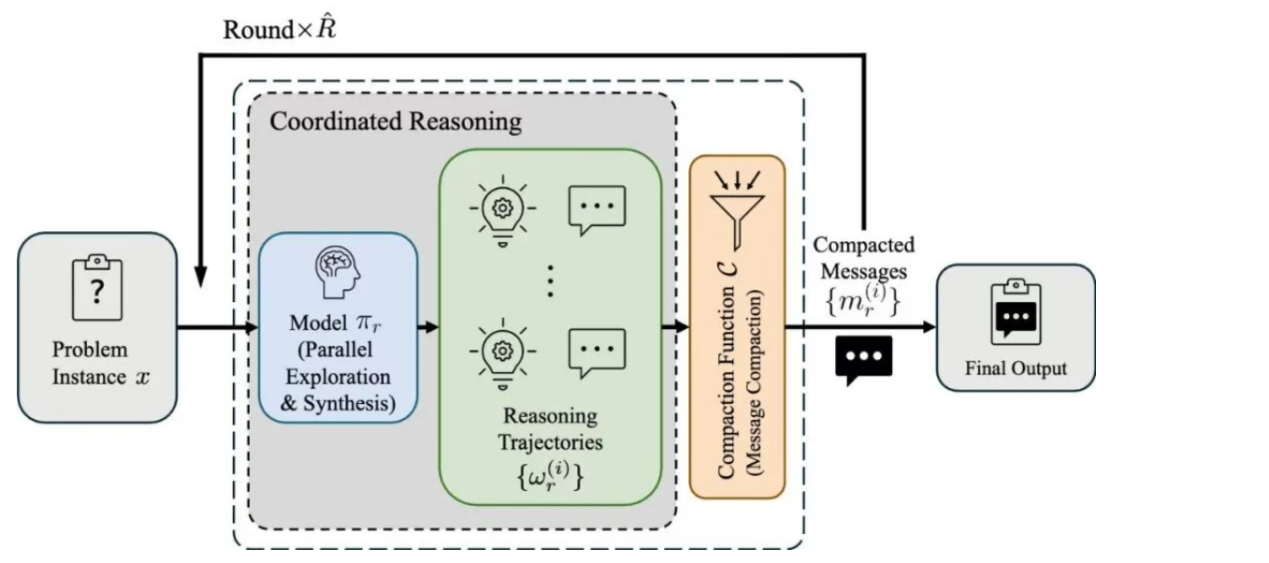
\includegraphics{images/image-0034.png}
\caption{PaCoRe 并行协同推理工作流}
\end{figure}

\hypertarget{ux4e8cux548cux57faux4e8eux641cux7d22ux7684ux65b9ux6cd5ux591aux667aux80fdux4f53ux65b9ux6cd5ux7684ux6bd4ux8f83}{%
\subsubsection{（二）和基于搜索的方法、多智能体方法的比较}\label{ux4e8cux548cux57faux4e8eux641cux7d22ux7684ux65b9ux6cd5ux591aux667aux80fdux4f53ux65b9ux6cd5ux7684ux6bd4ux8f83}}

和基于搜索的方法相比：基于搜索的推理是在每一步搜索多种路径、选择最优，以在解空间中寻找一条最优路径；而PaCoRe是并行展开多路推理直到最后，再进行视角的反复碰撞与融合，让模型自己``讨论''出一个收敛的结论。

和多智能体方法相比：多智能体架构中多个Agent往往有不同的System Prompt从而扮演不同角色，或为不同模型，这里只用了一个模型并行输出不同的推理过程，并在下一轮回馈给自身，相当于多个相同的Agent。

\hypertarget{ux4e09ux5173ux4e8eux5e76ux884cux63a8ux7406ux7684ux62d3ux5c55ux63a2ux8ba8}{%
\subsubsection{（三）关于并行推理的拓展探讨}\label{ux4e09ux5173ux4e8eux5e76ux884cux63a8ux7406ux7684ux62d3ux5c55ux63a2ux8ba8}}

除此架构外，其他并行推理架构还提出了一些不同的技术路径。

动态剪枝：在推理过程中，模型自身或一个专门的验证模型会实时评估当前路径的置信度，发现某条路径逻辑不通或概率降低时，自动``剪枝''终止该分支（Pruning），将计算资源集中到更有希望的路径上。但这对验证能力有较高的要求。

动态调整深度：系统会根据问题的复杂度，自动调整 thinking\_level（思考深度）。简单的问候直接回答，复杂的数学题则自动分配更多计算资源进行并行推演。

\hypertarget{ux53c2ux8003ux6587ux732e-126}{%
\subsection{参考文献}\label{ux53c2ux8003ux6587ux732e-126}}

\begin{itemize}
\tightlist
\item
  Zhu, J., Zhang, G., Ma, X., et al.~(2026). \href{https://arxiv.org/abs/2602.02486}{RE-TRAC: REcursive TRAjectory Compression for Deep Search Agents}. arXiv:2602.02486.
\item
  StepFun AI. (2025). \href{https://github.com/stepfun-ai/PaCoRe/blob/main/pacore_report.pdf}{PaCoRe: Parallel Coordinated Reasoning}. Technical report.
\end{itemize}

\clearpage

\hypertarget{ux601dux7ef4ux793eux4f1aux7406ux8bbaux8bbaux6587}{%
\section{思维社会理论（论文）}\label{ux601dux7ef4ux793eux4f1aux7406ux8bbaux8bbaux6587}}

\begin{quote}
本文是论文阅读笔记，内容代表对应论文方法或作者理解，不应直接视为领域共识或工程最佳实践。
\end{quote}

Google的相关研究指出，当前顶尖推理模型的强大推理能力，并非仅仅源于更长的思维链，还可能源于模型内部隐式地模拟了一个``思维社会''（Society of Thought）。模型在推理时，通过模拟不同视角、不同人格和专业背景的``隐形智能体''之间的对话、辩论和协作，从而实现了比单一视角更强的解决问题能力。

\hypertarget{ux4e00ux5177ux4f53ux8868ux73b0}{%
\subsection{一、具体表现}\label{ux4e00ux5177ux4f53ux8868ux73b0}}

\begin{enumerate}
\def\labelenumi{\arabic{enumi}.}
\item
  对话行为：推理模型频繁出现``提问-回答''、``视角切换''、``观点冲突''和``和解''等对话行为。相比之下，普通模型通常是平铺直叙的单向输出。利用Bales的交互过程分析（IPA），研究发现推理模型的对话行为不仅有信息交换，还包含``社会情感角色''的互动，例如表达反对或达成一致，这种互动随着问题难度的增加而变得更加频繁。
\item
  ``人格''与``专长''多样性：推理轨迹中包含多种隐式声音，这些声音在人格测试中表现出显著差异；模型也调用了不同领域的``专家''视角进行互动，避免了单一视角的偏见，促进了对解决方案空间的更有效探索。
\end{enumerate}

\hypertarget{ux4e8cux63a8ux7406ux80fdux529bux63d0ux5347ux7684ux76f8ux5173ux53d1ux73b0}{%
\subsection{二、推理能力提升的相关发现}\label{ux4e8cux63a8ux7406ux80fdux529bux63d0ux5347ux7684ux76f8ux5173ux53d1ux73b0}}

\begin{enumerate}
\def\labelenumi{\arabic{enumi}.}
\item
  激活``对话特征''能提升推理能力。如在模型中找到并增强了一个代表``对话中的惊讶/转折''（类似 ``Oh!'', ``Wait\ldots{}''）的特征，增强这一个对话特征，模型的数学推理准确率就大大提高，这证明了对话式的交互结构与推理能力之间存在因果关系。
\item
  即使只奖励最终答案的正确性（不奖励对话格式），模型在RL训练过程中也会自发地演化出提问、反思等对话行为。
\item
  训练方法启示：如果预先用``多智能体对话''数据对模型进行微调（SFT），再进行强化学习，模型的学习速度和最终性能都显著优于用``独白式思维链''微调的模型。这表明对话结构本身就是一种高效的推理脚手架。
\end{enumerate}

\hypertarget{ux53c2ux8003ux6587ux732e-127}{%
\subsection{参考文献}\label{ux53c2ux8003ux6587ux732e-127}}

\begin{itemize}
\tightlist
\item
  Du, Y., Li, S., Torralba, A., Tenenbaum, J. B., \& Mordatch, I. (2023). \href{https://arxiv.org/abs/2305.14325}{Improving Factuality and Reasoning in Language Models through Multiagent Debate}. arXiv:2305.14325.
\item
  Kim, J., Lai, S., Scherrer, N., Agüera y Arcas, B., \& Evans, J. (2026). \href{https://arxiv.org/abs/2601.10825}{Reasoning Models Generate Societies of Thought}. arXiv:2601.10825.
\end{itemize}

\clearpage


% 检索增强生成
\hypertarget{ux68c0ux7d22ux589eux5f3aux751fux6210}{%
\chapter{检索增强生成}\label{ux68c0ux7d22ux589eux5f3aux751fux6210}}

\hypertarget{ux68c0ux7d22ux589eux5f3aux751fux6210ux7684ux57faux672cux65b9ux6cd5}{%
\section{检索增强生成的基本方法}\label{ux68c0ux7d22ux589eux5f3aux751fux6210ux7684ux57faux672cux65b9ux6cd5}}

LLM尽管通用能力较强，但知识范围、实时性以及回答时知识定位的精确度都仍然有限。为此我们让模型在回答问题时实时检索，为回答提供参考。

\hypertarget{ux4e00ragux7684ux6807ux51c6ux6d41ux7a0b}{%
\subsection{一、RAG的标准流程}\label{ux4e00ragux7684ux6807ux51c6ux6d41ux7a0b}}

首先构建知识库，即对自然语言文本等非结构化数据的向量化存储。为了保存语义信息并方便后续的相似度检索，我们将文本裁切为片段，并训练一个嵌入模型，将这些片段分别转换为嵌入向量（embedding vector）并建立索引。

在生成时，我们会用Query（查询）向量在知识库中相似度检索，找到最相关的内容加入上下文（或将其所在的整篇文献加入上下文）。对于文本知识库，我们往往用余弦相似度，因为它更关注语义方向的相似性，而不受文本长度等无关因素的影响。而有时为了避免漏掉精确关键词，往往会和BM25等传统关键字检索方法结合，如finalScore~= (0.7~* vectorScore) + (0.3~* textScore)。

原始的RAG采取``先检索后生成''，即顺序架构：Query -\textgreater{} Retrieve -\textgreater{} Generate。

\hypertarget{ux4e8cux52a8ux6001ux51b3ux5b9aux8c03ux7528ux641cux7d22ux5de5ux5177}{%
\subsection{二、动态决定调用搜索工具}\label{ux4e8cux52a8ux6001ux51b3ux5b9aux8c03ux7528ux641cux7d22ux5de5ux5177}}

我们可以在模型的词表中加入 token，生成后即调用搜索API。可以通过在训练数据中加入调用示例，或者通过强化学习的方式让模型在自主探索中学会在需要搜索时生成 token，调用检索辅助完成任务。

\begin{enumerate}
\def\labelenumi{\arabic{enumi}.}
\tightlist
\item
  架构分类
\end{enumerate}

（1）条件架构：可以引入``判断器 (Judger/Router)''，根据问题的难度或类型决定是否检索，或如何检索，也可以通过强化学习的方式让模型自主学会判断是否搜索（即是否生成 token）。

（2）分支架构：并行执行多条路径，通过集成或排序来融合结果。

概率集成：将每个检索到的文档分别输入LLM计算生成概率，最后将多个文档对应的生成概率分布进行加权融合。

候选排序：让LLM基于每个文档分别生成答案，然后根据生成的置信度或相关性对这些答案进行排序，选择最好的一个。

（3）循环/迭代架构：检索和生成交替进行，形成闭环，Retrieve \textless-\textgreater{} Generate，适用于长文本生成或复杂多步推理。

交替迭代：生成一部分 -\textgreater{} 拿着生成的内容去检索新信息 -\textgreater{} 基于新信息继续生成 -\textgreater{} 循环。

主动触发：在生成过程中监测生成概率。如果 LLM 对当前生成的词``犹豫不决''（概率低），则立即触发检索，用检索到的信息``纠正''生成方向。

反思与自纠：训练LLM输出特殊的反思Token，判定是否需要检索，检索到的内容是否相关，生成的内容是否有用。

\begin{enumerate}
\def\labelenumi{\arabic{enumi}.}
\setcounter{enumi}{1}
\tightlist
\item
  训练方法
\end{enumerate}

（1）监督微调：需要高质量标注轨迹，且搜索操作本身的不可微性使得端到端优化变得困难。

（2）结合检索的强化学习：仅通过最终结果的奖励（Outcome-based Reward），让模型自主学会``思考-检索-再思考-回答''的交替流程，用PPO、GRPO等强化学习算法。

需要注意的是，在计算策略梯度时，轨迹y中既包含模型生成的 Token，也包含搜索引擎返回的固定Token。如果不加区分地训练，模型可能会试图``优化''检索到的文本，或者被检索内容的分布带偏。``检索''只是一个动作，模型通过强化学习（RL）的奖励机制学会的是何时输出标记。故我们运用掩码机制，把搜索到的文本Token（不包含 token）加上掩码，只以其他token作为RL优化的策略。

\hypertarget{ux4e09ux81eaux9002ux5e94rag}{%
\subsection{三、自适应RAG}\label{ux4e09ux81eaux9002ux5e94rag}}

在标准RAG中，在引入需要的信息的同时往往也引入了大量无关信息。为避免上下文无关信息的积累，可将检索到的信息分割成较小的块，每次输入一个块，并调用LLM回答，如此循环，直至得到需要的答案停止。由于KV Cache的存在，时间复杂度仍然是线性增长的（也就是和标准RAG一致），只要需要的信息不是在最后一个块里，理论上就能起到加速作用。

较大的块成功召回需要的信息的概率更大，但同时也会引入更多无关信息（干扰项）；较小的窗口虽能减少干扰，但要求模型在更多块中准确拒绝无关信息块，增加错误拒绝需要的信息块以及累计错误的风险。

\hypertarget{ux56dbux5f3aux63a8ux7406ux578bux4efbux52a1ux7684queryux5c55ux5f00}{%
\subsection{四、强推理型任务的Query展开}\label{ux56dbux5f3aux63a8ux7406ux578bux4efbux52a1ux7684queryux5c55ux5f00}}

在一些强推理型任务中，对Query也可以做推理展开，即先用原始Query检索一次，然后用LLM提取``有用证据''，写一个推理后的扩展查询/回答性段落作为新Query，再检索，然后将检索结果推理后才输入上下文。该过程用检索加强了对Query的理解，以更好地进行正式检索，引入推理以避免检索过度看表层语义。

本质上来说，该过程是进行了两轮``检索引导的显式推理''。需要一个辅助LLM，以免干扰原模型上下文。

\hypertarget{ux53c2ux8003ux6587ux732e-128}{%
\subsection{参考文献}\label{ux53c2ux8003ux6587ux732e-128}}

\begin{itemize}
\tightlist
\item
  《动手学大模型智能体》。
\item
  Jin, B., Zeng, H., Yue, Z., et al.~(2025). \href{https://arxiv.org/abs/2503.09516}{Search-R1: Training LLMs to Reason and Leverage Search Engines with Reinforcement Learning}. arXiv:2503.09516.
\end{itemize}

\clearpage

\hypertarget{ux7a00ux758fux68c0ux7d22}{%
\section{稀疏检索}\label{ux7a00ux758fux68c0ux7d22}}

稀疏检索即传统关键词检索方法，如BM25：

BM25 的核心思想是通过三个维度衡量查询 \(Q\) 与文档 \(D\) 的相关性：

\begin{enumerate}
\def\labelenumi{\arabic{enumi}.}
\item
  词频（TF, Term Frequency）：词在文档中出现的次数越多，相关性越高，但有饱和上限。
\item
  逆文档频率（IDF, Inverse Document Frequency）：包含该词的文档越少，该词的权重（信息量）越大。
\item
  文档长度归一化（Document Length Normalization）：同样的词频，出现在短文档中比出现在长文档中更重要。
\end{enumerate}

假设查询 \(Q\) 由单词 \(\{q_1, q_2, \ldots, q_n\}\) 组成，文档 \(D\) 的 BM25 得分计算公式如下：

\[
\mathrm{Score}(D,Q)=\sum_{i=1}^{n}\mathrm{IDF}(q_i)\cdot \frac{f(q_i,D)\cdot(k_1+1)}{f(q_i,D)+k_1\cdot(1-b+b\cdot\frac{|D|}{\mathrm{avgdl}})}
\]

其中：

\begin{itemize}
\tightlist
\item
  \(f(q_i,D)\)：单词 \(q_i\) 在文档 \(D\) 中的出现频率。
\item
  \(|D|\)：文档 \(D\) 的长度（单词数）。
\item
  \(\mathrm{avgdl}\)：语料库中文档的平均长度。
\item
  \(k_1\)：词频饱和参数，通常取 \(1.2\sim2.0\)，控制 TF 增长带来的得分上限。
\item
  \(b\)：长度惩罚参数，通常取 \(0.75\)，决定文档长度对得分的影响程度。
\end{itemize}

\(\mathrm{IDF}(q_i)\) 的标准计算方式为：

\[
\mathrm{IDF}(q_i)=\ln\left(\frac{N-n(q_i)+0.5}{n(q_i)+0.5}+1\right)
\]

其中 \(N\) 是语料库文档总数，\(n(q_i)\) 是包含单词 \(q_i\) 的文档数。

\hypertarget{ux53c2ux8003ux6587ux732e-129}{%
\subsection{参考文献}\label{ux53c2ux8003ux6587ux732e-129}}

\begin{itemize}
\tightlist
\item
  Robertson, S., \& Zaragoza, H. (2009). \href{https://doi.org/10.1561/1500000019}{The Probabilistic Relevance Framework: BM25 and Beyond}. Foundations and Trends in Information Retrieval, 3(4), 333-389.
\item
  Manning, C. D., Raghavan, P., \& Schutze, H. (2008). \href{https://nlp.stanford.edu/IR-book/html/htmledition/okapi-bm25-a-non-binary-model-1.html}{Introduction to Information Retrieval: Okapi BM25, a non-binary model}. Cambridge University Press.
\end{itemize}

\clearpage

\hypertarget{ux7a20ux5bc6ux68c0ux7d22ux4e0eux6df7ux5408ux68c0ux7d22}{%
\section{稠密检索与混合检索}\label{ux7a20ux5bc6ux68c0ux7d22ux4e0eux6df7ux5408ux68c0ux7d22}}

稠密检索，即利用Embedding向量检索的方法。相较于稀疏检索而言，稠密检索能更好地利用语义层面的信息。

\hypertarget{ux4e00ux5d4cux5165ux5411ux91cfux7684ux9009ux53d6}{%
\subsection{一、嵌入向量的选取}\label{ux4e00ux5d4cux5165ux5411ux91cfux7684ux9009ux53d6}}

\begin{enumerate}
\def\labelenumi{\arabic{enumi}.}
\tightlist
\item
  切成片段（Chunk）
\end{enumerate}

一般而言，一个嵌入向量会取256-1024 tokens，或者一个自然段，以包含一个完整的论点或逻辑段落。还可以计算相邻句子的相似度，如果相似度突降，说明话题变了，就在这里切。

为什么要这么做？如果把每一个词或每一句话单独做成向量，虽然粒度很细，但会因为缺乏上下文而导致语义偏离，检索时容易出错。如一个知识库把一个句子作为一个嵌入向量，有一个句子是``它崩溃了''。将其单独变为embedding向量，向量化后包含了``崩溃''的语义，但缺乏上下文，丢失了主语（是服务器崩溃，还是股市崩溃？）。检索时，在服务器、股市等很多场景检索时，这句话都会被检索到。也就是说，检索时会召回大量无关内容。而如果把整篇5000字的论文做成一个向量，要么需要很高的embedding维度（计算复杂度增大），要么在不改变维度的情况下把文章里不同内容的语义混合在向量里（向量的方向会变得模糊）。所谓``文档向量''，一般实际上就指的是片段对应的向量。

另外，我们不会硬生生切断，通常会设置10\%\textasciitilde20\%的重叠（例如50 Tokens），防止某个关键句子刚好被切在两块的连接处，导致语义断裂。

\begin{enumerate}
\def\labelenumi{\arabic{enumi}.}
\setcounter{enumi}{1}
\tightlist
\item
  切片的改进
\end{enumerate}

虽然切片是主流，但切片可能失去了上下文（例如，一个切片里写着``这个方案能将准确率提高20％''，但切片里没有写``这个方案''是什么）。对此有两种改进方法：（1）搜索到片段后，把其所在全文都输入给LLM；（2）在片段embedding时，将全文压缩后的摘要作为上下文输入供参考。

\hypertarget{ux4e8cux5d4cux5165ux5411ux91cfux7684ux5b58ux50a8ux4ecbux8d28}{%
\subsection{二、嵌入向量的存储介质}\label{ux4e8cux5d4cux5165ux5411ux91cfux7684ux5b58ux50a8ux4ecbux8d28}}

一般而言，被检索的嵌入向量保存在CPU内存中（或量化压缩后保存在CPU内存中）。如果数据量过大，可将索引向量压缩在内存，指向的原始文本数据存在SSD中。

由于嵌入向量在CPU内存中，在数据量不大的情况下，在推理时直接运用CPU计算可避免I/O阻塞耗时。如果数据量大、高并发必须使用GPU，则应将量化压缩后的索引向量集存入GPU显存，再取如Top-1000从CPU中取入GPU精确计算。

\hypertarget{ux4e09ux5d4cux5165ux6a21ux578bux7684ux67b6ux6784}{%
\subsection{三、嵌入模型的架构}\label{ux4e09ux5d4cux5165ux6a21ux578bux7684ux67b6ux6784}}

该方法采用双编码器架构（Bi-Encoder），通常基于 BERT 或 RoBERTa 等 Transformer 模型。

\begin{enumerate}
\def\labelenumi{\arabic{enumi}.}
\tightlist
\item
  编码（Encoding）：
\end{enumerate}

\begin{itemize}
\tightlist
\item
  文档编码：将语料库中的每个文档 \(d\) 输入文档编码器 \(E_D\)，取 \texttt{{[}CLS{]}} 位置的输出或所有 token 的平均池化，得到向量 \(\mathbf{v}_d \in \mathbb{R}^h\)。
\item
  查询编码：将用户问题 \(q\) 输入查询编码器 \(E_Q\)，得到向量 \(\mathbf{v}_q \in \mathbb{R}^h\)。
\end{itemize}

\[
\mathbf{v}_q=E_Q(q),\quad \mathbf{v}_d=E_D(d)
\]

\begin{enumerate}
\def\labelenumi{\arabic{enumi}.}
\setcounter{enumi}{1}
\tightlist
\item
  相似度计算（Similarity）：使用点积（Dot Product）或余弦相似度（Cosine Similarity）计算匹配分：
\end{enumerate}

\[
s(q,d)=\mathbf{v}_q^\top\mathbf{v}_d\quad \mathrm{or}\quad \frac{\mathbf{v}_q^\top\mathbf{v}_d}{\lVert\mathbf{v}_q\rVert\lVert\mathbf{v}_d\rVert}
\]

\hypertarget{ux56dbux5d4cux5165ux6a21ux578bux7684ux8badux7ec3}{%
\subsection{四、嵌入模型的训练}\label{ux56dbux5d4cux5165ux6a21ux578bux7684ux8badux7ec3}}

由于``选取最相关的一些文本加入上下文''运用了不可导的Top-K操作，嵌入模型无法直接和主LLM一起端到端训练，而需要另行训练。

\begin{enumerate}
\def\labelenumi{\arabic{enumi}.}
\tightlist
\item
  对比学习
\end{enumerate}

用语义相似的文本为正样本（如论文和它的摘要、论坛的问题和回答、新闻的标题和正文等），语义不同的为负样本（批次内非正样本均可视为负样本，此外还可以找辨析难度更大的困难样本，如讲水果中的苹果和苹果手机的段落）。

假设我们有一个查询 \(q\)（Query）和一个相关的文档 \(d^+\)（Positive Document），以及 \(N\) 个不相关的文档 \(d^-\)（Negative Documents）。

我们使用 InfoNCE Loss（Information Noise Contrastive Estimation）作为损失函数。这是目前训练 Embedding 最主流的公式：

\[
\mathcal{L}=-\log \frac{\exp(\mathrm{sim}(q,d^+)/\tau)}{\sum_{i=0}^{N}\exp(\mathrm{sim}(q,d_i)/\tau)}
\]

其中：

\begin{itemize}
\tightlist
\item
  \(\mathrm{sim}(u,v)\) 是两个向量的余弦相似度：
\end{itemize}

\[
\mathrm{sim}(u,v)=\frac{u^\top v}{\lVert u\rVert\lVert v\rVert}
\]

\begin{itemize}
\tightlist
\item
  \(d^+\) 是正样本。
\item
  \(d_i\) 包含 \(1\) 个正样本和 \(N\) 个负样本。
\item
  \(\tau\) 是温度系数（Temperature），用于控制模型对困难样本的敏感度。
\end{itemize}

\begin{enumerate}
\def\labelenumi{\arabic{enumi}.}
\setcounter{enumi}{1}
\tightlist
\item
  蒸馏生成模型的注意力分布
\end{enumerate}

字面相似度往往具有欺骗性，嵌入向量``是否相似''应当取决于内容逻辑，这是在复杂的生成过程中体现的。如：Query：``治疗阿尔茨海默病的新靶点。''文档A（字面相似）：一篇综述，标题包含``阿尔茨海默病治疗''，但内容全是老旧信息。文档B（字面不相似）：讨论``蛋白折叠异常与神经元坏死''，没提``阿尔茨海默''这个词，但内容逻辑正是通过解决蛋白折叠来治疗该病。

我们希望用下游任务的效用来监督上游检索的排序。尽管我们无法端到端优化嵌入模型，但可以让它生成的概率模仿生成器的Attention中各个token出现的概率，也就是运用蒸馏的方法：

第一步：获取生成器的``注意力分布'' \(P_{\mathrm{Teacher}}\)。

假设检索回了 \(K\) 个文档 \(\{D_1,D_2,\ldots,D_K\}\)。当生成器生成答案 \(Y\) 时，我们可以查看 Cross-Attention（或者 Decoder-Only 模型的 Self-Attention）层中的权重。

我们将生成器对第 \(i\) 个文档的所有 token 的注意力权重进行聚合（例如求和或取平均），得到该文档的重要性分数 \(A_i\)。然后进行归一化：

\[
P_{\mathrm{Gen}}(D_i\mid Q)=\frac{\exp(A_i/\tau)}{\sum_{j=1}^{K}\exp(A_j/\tau)}
\]

这个 \(P_{\mathrm{Gen}}\) 就是真理：它代表了``在生成答案时，第 \(i\) 篇文档实际上贡献了多少''。

第二步：获取检索器的``检索概率'' \(P_{\mathrm{Student}}\)。

检索器（通常是双塔模型）计算 Query 和 Document 的点积分数 \(S_i=E_Q\cdot E_{D_i}\)。我们也对它进行 Softmax 归一化：

\[
P_{\mathrm{Ret}}(D_i\mid Q)=\frac{\exp(S_i)}{\sum_{j=1}^{K}\exp(S_j)}
\]

第三步：计算损失并蒸馏（Distillation）。

我们要让检索器的分布 \(P_{\mathrm{Ret}}\) 尽可能接近生成器的分布 \(P_{\mathrm{Gen}}\)。通常使用 KL 散度（Kullback-Leibler Divergence）作为损失函数：

\[
\mathrm{Loss}=\mathrm{KL}(P_{\mathrm{Gen}}\Vert P_{\mathrm{Ret}})=\sum_i P_{\mathrm{Gen}}(D_i\mid Q)\log\frac{P_{\mathrm{Gen}}(D_i\mid Q)}{P_{\mathrm{Ret}}(D_i\mid Q)}
\]

关键点：这个 Loss 是可导的，可以通过梯度下降更新检索器的参数（即更新 Query Encoder 的权重），让检索器学会：``原来在这个问题下，虽然文档 B 只有 \(0.6\) 的相似度，但它应该排第一。''

\hypertarget{ux4e94ux6df7ux5408ux68c0ux7d22}{%
\subsection{五、混合检索}\label{ux4e94ux6df7ux5408ux68c0ux7d22}}

实践中，常采取稠密和稀疏索引结合的方法。如Claude-mem：查询先走Chroma向量检索（基于语义相似度的稠密检索），召回Top 100结果，再做90天时间窗口过滤，最后用SQLite（稀疏检索）按时间顺序补全/重排数据。

\hypertarget{ux53c2ux8003ux6587ux732e-130}{%
\subsection{参考文献}\label{ux53c2ux8003ux6587ux732e-130}}

\begin{itemize}
\tightlist
\item
  thedotmack. (2026). \href{https://github.com/thedotmack/claude-mem}{claude-mem GitHub repository}.
\item
  van den Oord, A., Li, Y., \& Vinyals, O. (2018). \href{https://arxiv.org/abs/1807.03748}{Representation Learning with Contrastive Predictive Coding}. arXiv:1807.03748.
\item
  Izacard, G., \& Grave, E. (2021). \href{https://arxiv.org/abs/2012.04584}{Distilling Knowledge from Reader to Retriever for Question Answering}. ICLR 2021.
\end{itemize}

\clearpage

\hypertarget{faissux52a0ux901f}{%
\section{Faiss加速}\label{faissux52a0ux901f}}

由于稠密检索需要遍历所有文档（片段）向量并进行逐个维度点乘，时间复杂度为O(n*d)。Faiss加速可以起到降低时间复杂度的作用。

\hypertarget{ux4e00ux67e5ux627eux6b21ux6570ux7684ux964dux4f4ek-meansux805aux7c7bux548cux5012ux6392ux7d22ux5f15ivf-inverted-file-index}{%
\subsection{一、查找次数的降低：K-means聚类和倒排索引（IVF, Inverted File Index）}\label{ux4e00ux67e5ux627eux6b21ux6570ux7684ux964dux4f4ek-meansux805aux7c7bux548cux5012ux6392ux7d22ux5f15ivf-inverted-file-index}}

IVF是常用的加速手段，其核心思想是``先粗筛，再精选''，类似于图书馆的分层检索。

工作机制：

\begin{enumerate}
\def\labelenumi{\arabic{enumi}.}
\item
  聚类：在训练阶段，利用 K-means 算法将整个向量空间划分为 \(k\) 个聚类（Voronoi Cells）。每个聚类中心被称为一个 Centroid。
\item
  建立倒排表：每一个原始向量都会被归类到离它最近的一个或多个聚类中心下，形成一个``倒排列表''。
\item
  查询加速：检索时，查询向量 \(q\) 首先与 \(k\) 个聚类中心对比，选出最近的 \(nprobe\) 个聚类，只在这几个聚类下的候选向量中进行精细计算。
\end{enumerate}

改进算法：

\begin{enumerate}
\def\labelenumi{\arabic{enumi}.}
\tightlist
\item
  倒排多索引（IMI, Inverted Multi-Index）
\end{enumerate}

这是一种通过``维度分解''实现的隐式多层聚类。

\begin{itemize}
\tightlist
\item
  数学逻辑：将 \(d\) 维向量切分为两半，每半部分分别进行聚类（假设各有 \(k\) 个中心）。
\item
  层级效果：通过这种组合，实际上产生了 \(k\times k=k^2\) 个虚拟桶。
\item
  优点：只需要存储 \(2k\) 个中心点，就能达到 \(k^2\) 级别的细分粒度。这在处理数十亿（Billions）级别的向量时非常强大。
\end{itemize}

\begin{enumerate}
\def\labelenumi{\arabic{enumi}.}
\setcounter{enumi}{1}
\tightlist
\item
  层次聚类树（IndexHierarchicalNSG / Multi-level K-means）
\end{enumerate}

在训练阶段，Faiss 可以通过多级 K-means 构建一棵树。

工作流：

\begin{enumerate}
\def\labelenumi{\arabic{enumi}.}
\item
  先将空间聚类成 \(100\) 个大类。
\item
  在每个大类内部，再聚类成 \(100\) 个子类。
\end{enumerate}

检索：像查字典一样，从树根向下搜索。

\hypertarget{ux4e8cux67e5ux627eux6b21ux6570ux964dux4f4eux7684ux53e6ux4e00ux65b9ux6cd5hnswhierarchical-navigable-small-worldux5206ux5c42ux5bfcux822aux5c0fux4e16ux754c}{%
\subsection{二、查找次数降低的另一方法：HNSW（Hierarchical Navigable Small World，分层导航小世界）}\label{ux4e8cux67e5ux627eux6b21ux6570ux964dux4f4eux7684ux53e6ux4e00ux65b9ux6cd5hnswhierarchical-navigable-small-worldux5206ux5c42ux5bfcux822aux5c0fux4e16ux754c}}

\begin{enumerate}
\def\labelenumi{\arabic{enumi}.}
\tightlist
\item
  基本思想
\end{enumerate}

NSW（导航小世界）：在一个图结构中，如果每个节点都与附近的节点相连（短程边），且存在少量跨度较大的随机连接（长程边），则整个图具有``小世界''特性。搜索时通过贪心算法，从一个起始点开始，不断移动到离目标最近的邻居。在RAG的背景下，这里的每个``节点''是一个向量，每个向量都和离它较近的向量在图中相连。

HNSW的改进：NSW在处理大规模数据时，搜索复杂度会退化。HNSW通过引入类似B+树的分层结构，每个在某层出现的节点在它上面的层必然也出现，搜索时不断``下降''，每次下一层的节点个数约为上一层的M倍（在插入节点时由概率确定该节点出现的最上层是哪一层，上一层的概率为下一层的1/M）。

例如：最高层有6，中间层有369，底层有123456789（一个序号代表一个向量离Query的距离）。从最高层的6出发，下沉到中间层，贪心可在很短的时间（常数时间，这是``小世界''特性带来的）内找到最近的3，再下沉到底层，又可以在常数时间找到1。可以证明，此时检索时间复杂度近似O(logN)，构建这个层级结构的时间复杂度近似O(NlogN)。

\begin{enumerate}
\def\labelenumi{\arabic{enumi}.}
\setcounter{enumi}{1}
\tightlist
\item
  检索工作流（O(logN)）
\end{enumerate}

阶段一：高层快速路由（Greedy Routing）。

\begin{itemize}
\tightlist
\item
  起始点：从最高层唯一的入口点开始。
\item
  贪心遍历：在每一层，只保留一个当前最优解，不断跳向比当前更靠近 \(q\) 的邻居。
\item
  目标：以极小的计算开销，跨越空间中的``荒漠''，迅速到达 \(q\) 所在的``绿洲''附近。
\end{itemize}

A. 高层贪心路由

原理：在 \(L_1\) 到 \(L_{\max}\) 层，不使用复杂的队列，只进行简单的贪心跳转。

为什么这么做？

\begin{itemize}
\tightlist
\item
  效率至上：高层节点少，误差容忍度高。快速下降到 \(L_0\) 才是核心任务。
\item
  小世界特性：根据 Watts-Strogatz 模型，小世界网络中通过少量的长程边（Long-range edges）即可实现极短的路径长度。高层边正是起到了长程边的作用。
\end{itemize}

B. 底层束搜索（Beam Search with \(C\) \& \(W\) Queues）

原理：在 \(L_0\) 层使用候选队列 \(C\)（小根堆）和结果队列 \(W\)（大根堆）进行扩展。

为什么这么做？

\begin{itemize}
\tightlist
\item
  克服局部最优：高维空间的向量分布非常复杂。贪心搜索（\(ef=1\)）很容易掉进``局部陷阱''。通过增大 \(efSearch\)，算法可以同时沿着多个可能的方向探索。
\item
  计算与精度的平衡：\(W\) 队列维护了目前最优秀的 \(efSearch\) 个候选者，它实际上划定了一个``动态搜索边界''。
\end{itemize}

阶段二：底层精细搜索（Beam Search at \(L_0\)）。

当下降到 \(L_0\) 层时，算法从贪心策略切换为基于两个优先级队列的束搜索（类似于宽度优先搜索的变种）：

我们采用类似广度优先的算法，但不同的是，这里只把最小邻居（而非所有邻居）压入待访问队列C，使得算法具备一定的贪心性；BFS中的``访问''，也被改成了``加入结果队列W''：

数据结构准备：

\begin{itemize}
\tightlist
\item
  候选队列 \(C\)（Candidate Set）：小根堆，存储``待探索''的节点，离 \(q\) 越近优先级越高。
\item
  结果队列 \(W\)（Result Set）：大根堆，存储``目前为止最接近 \(q\)''的 \(efSearch\) 个节点。
\end{itemize}

循环迭代：

\begin{itemize}
\tightlist
\item
  从 \(C\) 中弹出距离 \(q\) 最近的节点 \(c\)。
\item
  获取 \(c\) 的所有邻居 \(e\)。
\item
  距离判定：如果 \(\mathrm{dist}(e,q)\) 小于 \(W\) 中最远节点的距离（即大根堆堆顶），则将 \(e\) 同时压入 \(C\) 和 \(W\)。
\item
  动态调整：如果 \(W\) 超过了 \(efSearch\) 大小，弹出堆顶最远的点。
\end{itemize}

收敛条件：

\begin{itemize}
\tightlist
\item
  当 \(C\) 为空，或者 \(C\) 中最近的节点已经比 \(W\) 中最远的节点还要远时，搜索停止。
\end{itemize}

为什么这样选取收敛条件：

\begin{itemize}
\tightlist
\item
  图的单调性假设：在导航小世界图中，我们假设如果当前能看到的最好机会（\(C\) 的堆顶）都比你已经握在心里的最差结果（\(W\) 的堆顶）还要差，那么在图的更深处找到更好结果的概率已经很小。
\item
  大幅减少计算量：这避免了对图进行全量遍历，是 HNSW 实现毫秒级响应的核心。
\end{itemize}

\begin{enumerate}
\def\labelenumi{\arabic{enumi}.}
\setcounter{enumi}{2}
\tightlist
\item
  构建层级结构工作流（O(NlogN)）
\end{enumerate}

第一步：确定最大层级 \(l\)。

每个节点在插入前，都会被赋予一个最高可见层级 \(l\)。这通过泊松分布或指数分布随机生成：

\[
l=\lfloor-\ln(\mathrm{unif}(0,1))\cdot m_L\rfloor
\]

物理意义：大部分节点只存在于底层（\(L_0\)），只有极少数幸运儿能登上高层。这构成了典型的``金字塔''结构。

第二步：跨层寻找入口点。

系统从整个索引的全局入口点（Enter Point，预定义的最高层节点）开始，自顶向下搜索：

\begin{enumerate}
\def\labelenumi{\arabic{enumi}.}
\item
  在每一层执行贪婪搜索：检查当前节点的邻居，找到离 \(\mathbf{v}_{new}\) 最近的一个邻居。
\item
  将该邻居作为下一层的起始点，继续下沉。
\item
  注意：在进入 \(l\) 层之前，这个过程不建立连接，只为了快速定位。
\end{enumerate}

为什么这么做？

\begin{itemize}
\tightlist
\item
  快速收敛：高层图相当于空间的``摘要''。在稀疏图中，贪心搜索能以极少的计算量（跨越式地）快速逼近查询向量所在的局部区域。
\item
  消除冗余：在高层没必要找 Top-K，因为高层的目的是``导航''而非``精检''。
\end{itemize}

第三步：逐层建立连接（Layer \(i\in[0,l]\)）。

一旦进入 \(l\) 层及以下层级，系统开始真正的``拉帮结派''：

\begin{enumerate}
\def\labelenumi{\arabic{enumi}.}
\item
  确定候选者：在当前层进行类似检索的搜索，维护一个大小为 \(efConstruction\) 的候选节点集合。
\item
  选择邻居（\(M\) 个）：从候选中选出 \(M\) 个点与 \(\mathbf{v}_{new}\) 建立双向边。
\item
  启发式连接策略（Heuristic）：这是 HNSW 的关键。系统不一定只选最近的 \(M\) 个点，而是会考虑这些点是否``扎堆''。
\end{enumerate}

\begin{itemize}
\tightlist
\item
  策略：如果候选点 \(A\) 离 \(\mathbf{v}_{new}\) 较近，但 \(A\) 已经和已选中的邻居 \(B\) 靠得太近，系统可能会跳过 \(A\)，转而选择一个稍微远一点但方向不同的点。
\item
  目的：确保连接具有方向多样性，避免搜索时陷入``死胡同''。
\end{itemize}

为什么这么做？

\begin{itemize}
\tightlist
\item
  解决``孤岛''效应：如果只连最近的邻居，节点会倾向于形成密集的簇（Cluster），而簇与簇之间缺乏连接。一旦搜索进入一个簇，就很难跳出来。
\item
  模拟相对邻域图（Relative Neighborhood Graph）：这种策略保证了图的全局连通性。即使搜索点离目标较远，也能通过这些``跨度较大''的边快速横跨空间。
\end{itemize}

\hypertarget{ux4e09ux70b9ux79efux8ba1ux7b97ux548cux5411ux91cfux5b58ux50a8ux590dux6742ux5ea6ux7684ux964dux4f4eux4e58ux79efux91cfux5316pq-product-quantization}{%
\subsection{三、点积计算和向量存储复杂度的降低：乘积量化（PQ, Product Quantization）}\label{ux4e09ux70b9ux79efux8ba1ux7b97ux548cux5411ux91cfux5b58ux50a8ux590dux6742ux5ea6ux7684ux964dux4f4eux4e58ux79efux91cfux5316pq-product-quantization}}

子空间切分：将 \(d\) 维向量切分为 \(m\) 个子向量，每个子向量的维度为 \(d/m\)。

\[
x=[x_1,x_2,\ldots,x_m]
\]

子空间量化：对每个子空间的向量分别进行 K-means 聚类。通常每个子空间聚成 \(k^*=2^8=256\) 个类。这样每个子向量就可以用一个 8-bit 的索引（0-255）来表示。

编码压缩：一个原先需要 \(d\times32\) bits（浮点数）的向量，现在只需要 \(m\times8\) bits。压缩比可达 30-100 倍。

非对称距离计算（ADC）：当查询向量 \(q\) 到来时，系统会预先计算 \(q\) 的每个子向量到该子空间 256 个聚类中心的距离，生成一个距离查找表（Distance Look-up Table）。

\[
D(q,x)\approx \sum_{i=1}^{m}\mathrm{LUT}_i[\mathrm{code}_i(x)]
\]

这样我们不需要把Query和n个d维向量逐个点积，而是只需要和m*256个d/m维聚类中心向量点积，对于每个d维向量来说，它的每个子向量（只需要存聚类中心的ID）和Query的点积就是其聚类中心和Query的点积，只需要去距离查找表中查到每个子向量的点积再相加即可。

\hypertarget{ux53c2ux8003ux6587ux732e-131}{%
\subsection{参考文献}\label{ux53c2ux8003ux6587ux732e-131}}

\begin{itemize}
\tightlist
\item
  Babenko, A., \& Lempitsky, V. (2012). \href{https://ieeexplore.ieee.org/document/6248018}{The Inverted Multi-Index}. CVPR 2012.
\item
  Johnson, J., Douze, M., \& Jegou, H. (2017). \href{https://arxiv.org/abs/1702.08734}{Billion-scale similarity search with GPUs}. IEEE Transactions on Big Data.
\item
  Malkov, Y. A., \& Yashunin, D. A. (2018). \href{https://arxiv.org/abs/1603.09320}{Efficient and robust approximate nearest neighbor search using Hierarchical Navigable Small World graphs}. IEEE TPAMI.
\end{itemize}

\clearpage

\hypertarget{ux91cdux6392ux5e8fux4e0eux7cbeux70bc}{%
\section{重排序与精炼}\label{ux91cdux6392ux5e8fux4e0eux7cbeux70bc}}

\hypertarget{ux4e00ux91cdux6392ux5e8fux5668}{%
\subsection{一、重排序器}\label{ux4e00ux91cdux6392ux5e8fux5668}}

\begin{enumerate}
\def\labelenumi{\arabic{enumi}.}
\tightlist
\item
  全量重排序
\end{enumerate}

前面的稀疏和稠密检索可以让我们获得Top-K分数的文档（片段），但都主要集中在整个文档（片段）向量的整体语义上，为了速度牺牲了精度。为此，我们还需要进一步在token级别进行精细化调整，即用重排序器，在检索出的 Top-K（例如前100个）文档上进行排序。具体方法有：

（1）LLM评估法

（2）交叉编码器法

输入构造：将查询 \(q\) 和候选文档 \(d\) 拼接成一个序列，中间用分隔符隔开：

\[
\mathrm{Input}=[\mathrm{CLS}]\oplus q\oplus[\mathrm{SEP}]\oplus d\oplus[\mathrm{SEP}]
\]

全注意力交互（Full Self-Attention）：将拼接后的序列输入 Transformer。由于 Self-Attention 机制，查询中的每个 token 都能注意到文档中的每个 token。这使得模型能理解复杂的逻辑关系（如否定词``不''、``但是''）。

评分输出：通常取 \texttt{{[}CLS{]}} 标记的输出向量，经过一个全连接层（Linear Layer），输出一个标量分数 \(s\in[0,1]\)（通常经过 Sigmoid）。

\[
\mathrm{Score}(q,d)=\sigma(W\cdot \mathrm{Transformer}(\mathrm{Input})_{\mathrm{CLS}}+b)
\]

可以看到，这里并非Query对文档用互注意力（Bi-Encoder），而是Query和文档拼接后用自注意力打分（Cross-Encoder）。最后取 \texttt{{[}CLS{]}} 标记对应的全局注意力向量，追求极致的精度。（注：\(W\) 为 \(1\times d_{\mathrm{model}}\) 维，和 \texttt{{[}CLS{]}} token 向量的 \(d_{\mathrm{model}}\times 1\) 维相乘为标量）

为什么选择交叉编码器：

\begin{itemize}
\tightlist
\item
  双编码器（Bi-Encoder）：

  \begin{itemize}
  \tightlist
  \item
    流程：Query -\textgreater{} Vector \(V_q\)，Doc -\textgreater{} Vector \(V_d\)。
  \item
    计算：\(V_q \cdot V_d\)。
  \item
    痛点：Query 和 Doc 在生成向量时是互不可见的。所有的语义必须被压缩到一个固定维度的向量中（Vector Bottleneck）。例如，``苹果''这个词，在生成向量时必须同时隐含``水果''和``公司''的含义，非常模糊。
  \end{itemize}
\item
  交叉编码器（Cross-Encoder）：

  \begin{itemize}
  \tightlist
  \item
    流程：将 Query 和 Doc 拼接后送入模型。
  \item
    优势：Query 和 Doc 在模型的第一层就开始交互。
  \end{itemize}
\end{itemize}

``互不可见''指的就是：在生成 \(V_d\) 的那一刻，模型不知道 \(Q\) 是什么；在生成 \(V_q\) 的时刻，模型不知道 \(D\) 是什么。它们是独立编码的。

假设有一篇文档 \(D\)：``苹果发布了新财报，股价大涨。''

\begin{itemize}
\tightlist
\item
  场景 A（Cross-Encoder，无瓶颈）：

  \begin{itemize}
  \tightlist
  \item
    Query：``好吃的水果有哪些？'' -\textgreater{} 拼接后模型看到``水果''和``股价''，直接打低分。
  \item
    Query：``科技公司动态'' -\textgreater{} 拼接后模型看到``科技''和``股价''，打高分。
  \item
    模型在交互中动态理解了语义。
  \end{itemize}
\item
  场景 B（Bi-Encoder，有瓶颈）：

  \begin{itemize}
  \tightlist
  \item
    文档 \(D\) 必须被压缩成一个静态向量 \(V_d\)。
  \item
    这个 \(V_d\) 必须同时通过 768 个数字来表达``苹果''、``公司''、``赚钱''、``科技''等所有含义。
  \item
    多义词灾难：

    \begin{itemize}
    \tightlist
    \item
      如果 \(V_d\) 过分强调``科技''，那遇到 Query ``苹果（水果）''时，虽然语义不符，但因为都含有``Apple''这个词的嵌入信息，向量距离可能还是很近（产生幻觉/误召回）。
    \item
      如果 \(V_d\) 试图中庸，既像水果又像科技，那它可能离``纯粹的水果''和``纯粹的科技''都有一段距离，导致谁都搜不到它。
    \end{itemize}
  \end{itemize}
\end{itemize}

总结：Vector Bottleneck 指的是：无论句子多长、含义多丰富、多歧义，双编码器都强行将其压缩进一个固定大小的向量中。由于缺乏查询时的上下文（Context），这个向量只能是一个``模糊的平均值''，丢失了细粒度的语义匹配能力。
而如果用交叉编码器，模型在Embedding时可直接将Query和文档拼接，根据Query确定把文档的哪些内容放进Embedding。但缺点是这样文档的Embedding依赖于Embedding，必须在每次给出Query后都在线计算，而无法提前单独对文档进行Embedding操作。

\begin{enumerate}
\def\labelenumi{\arabic{enumi}.}
\setcounter{enumi}{1}
\tightlist
\item
  chunk重排序
\end{enumerate}

在数据量大、对延时要求高、算力相对不足等情形下，对所有的论文进行整个文档的token级计算并不现实，往往每篇论文只能取几个较小的chunk送进重排序器（如果是论文检索等场景，往往除了chunk之外还会加上摘要一并送入重排序器）。一般而言，切分chunk的方法有：

（1）按自然段/一定token数切分：每段或每一定token数为一个chunk，最简便，但有时会丢失一些上下文信息，或出现冗余信息。可以通过加入压缩后的上下文、与相邻chunk 20\%重叠的方式一定程度上解决丢失上下文信息的问题，保证连续性。

（2）按句子切分再合并：先按句子切分，再计算每一句与下一句的embedding向量间的相似度。若高于阈值，则将下一句合并入该句所在chunk；否则二者分入不同chunk。这样可以得到若干chunk。

切分完毕后，计算Query与每个小chunk的embedding向量间的相似度，取每篇论文TopK的chunk，送进重排序器。

\hypertarget{ux4e8cux7cbeux70bcux5668}{%
\subsection{二、精炼器}\label{ux4e8cux7cbeux70bcux5668}}

检索到的文档往往包含大量无关噪声，直接输入生成器会导致Token浪费甚至产生幻觉。精炼器的目标是提高``信噪比''，故常用精炼器进行精炼后再加入上下文窗口。

精炼方法：

\begin{enumerate}
\def\labelenumi{\arabic{enumi}.}
\item
  抽取式精炼：使用一个轻量级的打分模型（甚至可以是另一个 Cross-Encoder）对每个句子评分，判断其是否包含回答问题所需的关键信息。
\item
  摘要式精炼：让LLM或小型BERT模型对检索到的内容生成摘要。
\item
  LLMLingua压缩：用LLM预测对应token，越能被轻易预测，该token信息量（困惑度）越小，越应压缩。
\end{enumerate}

\[
\mathrm{Keep}(x_t)=\mathbf{1}\!\left[-\log P\!\left(x_t \mid x_{1:t-1}\right)>\tau\right]
\]

\hypertarget{ux53c2ux8003ux6587ux732e-132}{%
\subsection{参考文献}\label{ux53c2ux8003ux6587ux732e-132}}

\begin{itemize}
\tightlist
\item
  Nogueira, R., \& Cho, K. (2019). \href{https://arxiv.org/abs/1901.04085}{Passage Re-ranking with BERT}. arXiv:1901.04085.
\item
  Reimers, N., \& Gurevych, I. (2019). \href{https://arxiv.org/abs/1908.10084}{Sentence-BERT: Sentence Embeddings using Siamese BERT-Networks}. EMNLP 2019.
\item
  Xu, F., Shi, W., \& Choi, E. (2023). \href{https://arxiv.org/abs/2310.04408}{RECOMP: Improving Retrieval-Augmented LMs with Compression and Selective Augmentation}. ICLR 2024.
\item
  Jiang, H., Wu, Q., Lin, C.-Y., Yang, Y., \& Qiu, L. (2023). \href{https://arxiv.org/abs/2310.05736}{LLMLingua: Compressing Prompts for Accelerated Inference of Large Language Models}. EMNLP 2023.
\end{itemize}

\clearpage


% 上下文与记忆
\hypertarget{ux4e0aux4e0bux6587ux4e0eux8bb0ux5fc6}{%
\chapter{上下文与记忆}\label{ux4e0aux4e0bux6587ux4e0eux8bb0ux5fc6}}

\hypertarget{ux6a21ux578bux7684ux8bb0ux5fc6}{%
\section{模型的记忆}\label{ux6a21ux578bux7684ux8bb0ux5fc6}}

\hypertarget{ux4e00ux77edux671fux8bb0ux5fc6ux4e0aux4e0bux6587}{%
\subsection{一、短期记忆（上下文）}\label{ux4e00ux77edux671fux8bb0ux5fc6ux4e0aux4e0bux6587}}

短期记忆是大模型执行任务时对当前任务上下文的记忆，对应``上下文学习''，其底层实现是注意力中存储的KV Cache，任务结束后即清空。

由于硬件显存有限，大模型的上下文窗口长度有限，如果超出长度就必须采取一些机制。对于短期记忆自身而言，可以采取的措施例如：

\begin{enumerate}
\def\labelenumi{\arabic{enumi}.}
\item
  滑动窗口：保留最近的K轮对话。
\item
  摘要：对于更早的内容，生成摘要，并``遗忘''原内容，一般和滑动窗口配合使用。摘要会暂时储存在内存中，并加入后续对话的上下文窗口。
\end{enumerate}

后续还会有和长期记忆配合的一些其他方法。

\hypertarget{ux4e8cux957fux671fux8bb0ux5fc6}{%
\subsection{二、长期记忆}\label{ux4e8cux957fux671fux8bb0ux5fc6}}

我们可以通过向量数据库的形式，将记忆内容嵌入为语义向量，保存在大容量介质（如硬盘）中。例如，OpenClaw将记忆存储在工作区的特定markdown文件中。在运用时，根据请求用向量相似度在数据库中检索，获取最相关的内容，也可以通过提示词让模型以其他方式灵活调取。记忆内容可以包括历史问答及其摘要、垂直领域知识、执行动作的历史及经验教训、用户偏好等。

在上下文超过短期记忆上限时，我们可以将最早的历史信息（或只存其摘要）移动到长期记忆中，在后续如果被检索到（即需要这些信息）则再加入短期记忆。

由于长期记忆读写速度慢，我们一般不会每次对话都访问，而是在初始化（开始工作前）、检索（遇到一定的问题或场景，LLM判断需要调用记忆）或归档（项目做完打包结项）等时候按需要调用。

长期记忆可以分层，如OpenClaw包括一个大数据库和一个精选过的最重要的记忆（如用户偏好、重要决定等），每次涉及与用户对话时都会调取精选记忆。以Claude-mem为例，其采取了``渐进式披露''的方法，在通过检索方法（稠密检索、稀疏检索）得到若干条记忆条目后，不立即全部注入上下文，而是分层处理。具体而言，就是在建立记忆时，就分为如下三层，从而在调用时分层读取：

Layer 1：Search（索引层）：一个``轻量索引''，每一行包括该条记忆的ID、时间、类别、标题、token成本，例如：\textbar{} \#2102\textbar{} Oct 20 \textbar{} problem-solution \textbar{} Fixed timeout in CI \textbar{} 100 tokens \textbar。如gotcha表示这是个坑，problem-solution表示这是曾经的问题与解法等。对于检索到的条目，将它们的索引层注入主模型，模型看标题和类型就能判断：这一条是否有必要调用更贵的Layer 2 / Layer 3。（这里和前面的检索的不同点在于，检索是运用固定的检索算法，因而比较粗略，无法处理精细语义；这里虽然只有少量浓缩信息，但模型可以根据需要灵活判断）

Layer 2：Timeline（时间线层）：事件记忆，类似于日志。当模型在Layer 1中选定ID后，对于每个ID，拉出它的前后几条时间线，看看这步操作的前后都发生了什么。

Layer 3：Get Observations（详情层）：对Layer 1中选定的ID，如果经过读取Layer 2后，模型仍认为需要更多信息，则会拉取该ID对应的完整结构化内容。例如：

\begin{verbatim}
#2543 Hook timeout: 60s too short for npm install

Date: Oct 26, 2025 2:14 PM
Type: gotcha
Project: claude-mem

Narrative:
Discovered that the default 60-second hook timeout is insufficient for npm
install operations, especially with large dependency trees or slow network
conditions. This causes SessionStart hook to fail silently, preventing context
injection.

Facts:
- Default timeout: 60 seconds
- npm install with cold cache: ~90 seconds
- Configured timeout: 120 seconds in plugin/hooks/hooks.json:25

Files Modified:
- plugin/hooks/hooks.json

Concepts: hooks, timeout, npm, configuration
\end{verbatim}

总而言之，这里的结构化信息包括：

Narrative（叙事）：

用自然语言描述``发生了什么、问题是什么、影响是什么''，方便 Agent 理解上下文。

Facts（事实清单）：

关键数值、配置项、结论，方便做逻辑推理。

Files Modified / Files Read：

直接告诉 Agent：这个观察跟哪些文件有关，不用自己去猜。

Concepts（概念标签）：

用于语义检索，例如``hooks / timeout / npm''等，方便后续基于概念检索。

官方示例中，典型的模式是：Layer 1：limit=10条索引；Layer 2：选2--3个ID拉时间线；Layer 3：对于其中有必要的，再完整观察。下面举一个例子：

Layer 1：调用 \texttt{search(\{\ query:\ "hook\ timeout",\ limit:\ 10\ \})}

得到 3 条相关记忆的索引：

\#2543：Hook timeout: 60s too short

\#2891：Hook timeout configuration

\#2102：Fixed timeout in CI

Layer 2：Claude判断\#2543最相关，调用 \texttt{timeline(\{\ anchor:\ 2543,\ depth\_before:\ 3,\ depth\_after:\ 3\ \})}，看到：

之前：尝试过哪些超时配置

当前：把 60s 改成 120s

之后：CI 中也统一了这个配置

Layer 3：如果觉得需要更多细节，再调用 \texttt{get\_observations(\{\ ids:\ {[}2543,\ 2102{]}\ \})}

得到完整的叙事、事实、修改文件列表等，用于当前决策。

\hypertarget{ux4e09ux5185ux5b58}{%
\subsection{三、内存}\label{ux4e09ux5185ux5b58}}

AI Agent（智能体）的运行过程中，系统内存（System RAM / CPU Memory）扮演的是``调度员''和``中转站''的角色，是连接硬盘（数据库）和显卡（LLM）的桥梁。我们写的Agent程序就是在内存中运行的。

对于一些信息，容量超出了短期记忆，但调用频次又较高，难以接受长期记忆的检索效率。因此，我们可以在程序里建立数据结构，在内存里存储。如下面的两个例子。

\begin{enumerate}
\def\labelenumi{\arabic{enumi}.}
\tightlist
\item
  按重要性保留历史信息
\end{enumerate}

设立评分机制（如TF-IDF、注意力权重、打分模型），判断历史信息的重要程度，保留最重要的K条（如K=5或10）内容，适合关键信息分散在较长时间段的任务。

在数据结构的实现上，我们可以在程序中编写一个动态变化的堆，每增加一条对话，就评判其重要性权重，根据分数加入到堆。堆只保留分数最高的K条。当第K+1条数据进来，如果分数不够高，直接丢弃；如果比堆里最低的高，就从堆里去除原来最低的，把它放进去。在下一次问答前，再将堆中的内容加入短期记忆即上下文中。关于为什么这个过程必须在堆而不是上下文里实现，可以参考下面的例子：

你的上下文窗口只能装 3 条记忆。

不使用堆（直接进上下文）：

\begin{enumerate}
\def\labelenumi{\arabic{enumi}.}
\tightlist
\item
  用户说：``我叫小明。'' -\textgreater{} 存入上下文（剩 2 空位）。
\item
  用户说：``今天天气不错。'' -\textgreater{} 存入上下文（剩 1 空位）。
\item
  用户说：``吃个苹果。'' -\textgreater{} 存入上下文（满员）。
\end{enumerate}

突发情况：用户突然说：``我对青霉素过敏！''

此时上下文已经塞满了前 3 条废话。如果要加这条最重要的，你需要复杂的逻辑去``擦除''上下文里的某一条。在 Prompt 字符串里做``查找替换''是非常麻烦且低效的。

在堆里操作：

\begin{itemize}
\tightlist
\item
  操作对象：Python 里的 List/Object。
\item
  代价：纳秒级 CPU 时间，0 块钱。
\item
  灵活性：你可以随意增加、删除、修改权重、重新排序。
\end{itemize}

在上下文里操作：

\begin{itemize}
\tightlist
\item
  操作对象：发给 API 的 Prompt 字符串。
\item
  代价：Token 是按量计费的。一旦你把 Prompt 发出去，就覆水难收。
\end{itemize}

堆（Heap）是草稿纸，上下文（Context）是最终试卷。

\begin{itemize}
\tightlist
\item
  你可以在草稿纸上反复计算、涂改、比较，决定哪道题是重点（在堆里根据分数排序、替换）。
\item
  但是当你把答案写到试卷上（放入 Context Window）并交卷（发送给 LLM）之后，就不能改了。
\end{itemize}

\begin{enumerate}
\def\labelenumi{\arabic{enumi}.}
\setcounter{enumi}{1}
\tightlist
\item
  生成摘要
\end{enumerate}

前面提到过，当对话超出上下文限制时，让LLM为之前的对话生成一段摘要，注入之后的上下文窗口。写成程序语句如\texttt{summary=agent.ask(massage)}，\texttt{massage}里包含了要求生成摘要的prompt，这里的\texttt{summary}就暂时存在内存中，等待被注入新的上下文。

summary并非简单把长文本变成短文本，这会丢失大量细节。它应当保留模型对原始对话的``隐性理解''，就像把一本厚书压缩成一个``记忆卡片''，模型读了卡片就能回忆起整本书的内容。例如OpenAI Codex的策略是，对于代码项目中的对话，当上下文窗口满时，用一个小项目列表替换前文，概括前面都执行了什么。

\hypertarget{ux53c2ux8003ux6587ux732e-133}{%
\subsection{参考文献}\label{ux53c2ux8003ux6587ux732e-133}}

\begin{itemize}
\tightlist
\item
  《动手学大模型智能体》。
\item
  OpenClaw. (2026). \href{https://github.com/openclaw/openclaw}{OpenClaw GitHub repository}.
\item
  thedotmack. (2026). \href{https://github.com/thedotmack/claude-mem}{claude-mem GitHub repository}.
\end{itemize}

\clearpage

\hypertarget{ux4e0aux4e0bux6587ux7ba1ux7406}{%
\section{上下文管理}\label{ux4e0aux4e0bux6587ux7ba1ux7406}}

\hypertarget{ux4e00ux63d0ux9ad8ux7f13ux5b58ux547dux4e2dux7387}{%
\subsection{一、提高缓存命中率}\label{ux4e00ux63d0ux9ad8ux7f13ux5b58ux547dux4e2dux7387}}

对于Agent Loop来说，每跑一圈都要把之前的对话历史（包括那些冗长的报错信息、文件内容）重新发给模型，将导致计算复杂度平方级增长。可以采用缓存策略让KV Cache尽可能命中。

从缓存角度，上下文从前到后往往分为：全局缓存（System指令、工具定义）；任务/项目级缓存（如CLAUDE.md，AGENT.md）；会话级缓存（历史对话）；当前会话消息（用户输入、环境反馈结果等）。尽量把静态内容放在前面，动态内容放在后面。对于前面不变的部分，服务器就不需要重新计算，直接调取缓存中的历史记录。

这样可以让长对话的成本从平方级增长降到线性级。但任何改变System指令/工具定义/历史对话等的操作都会导致缓存失效，如中途换模型、切换工作目录、修改权限配置、改变MCP工具列表等。为尽可能确保缓存命中，有以下方法：

\begin{enumerate}
\def\labelenumi{\arabic{enumi}.}
\item
  保持提示前缀稳定。由于LLM的自回归特性，即使是单个标记的差异也会使该标记之后的缓存失效。例如，一些配置修改、工具变更尽量通过在input中附加一条信息，如system propmt的修改可用类似于的形式实现，而非完全抛弃缓存。一个常见的错误是在系统提示的开头包含时间戳，尤其是精确到秒的时间戳，这会大大降低缓存命中率。
\item
  使会话上下文只追加。避免修改之前的操作或观察。要当心的是许多编程语言和库在序列化JSON对象时不保证键顺序的稳定性，这可能会悄无声息地破坏缓存。上下文精简尽量在缓存本来就要未命中的时候进行。
\item
  在需要时明确标记缓存断点。某些模型提供商或推理框架不支持自动增量前缀缓存，而是需要在上下文中手动插入缓存断点。在分配这些断点时，要考虑潜在的缓存过期问题，并至少确保断点包含系统提示的结尾。
\end{enumerate}

\begin{figure}[htbp]
\centering
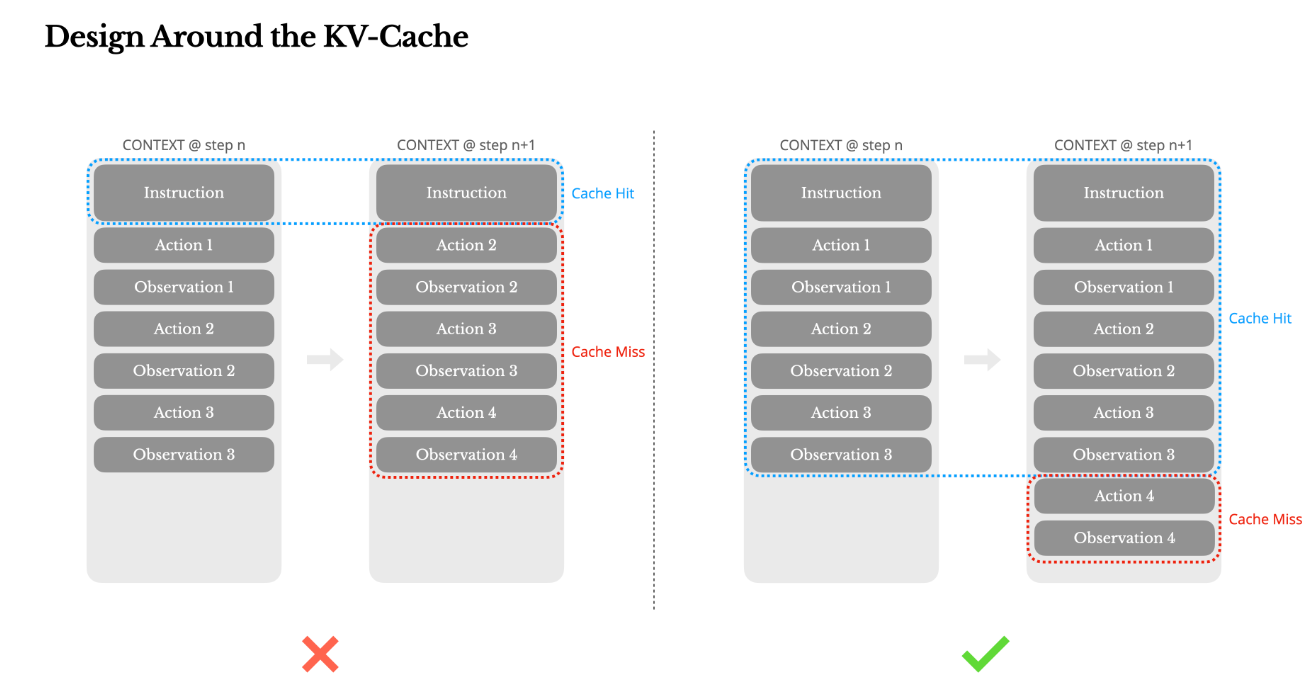
\includegraphics{images/image-0035.png}
\caption{KV Cache 缓存命中与未命中对比}
\end{figure}

\hypertarget{ux4e8cux5de5ux5177ux7ba1ux7406}{%
\subsection{二、工具管理}\label{ux4e8cux5de5ux5177ux7ba1ux7406}}

随着Agent能力的增强，其行动空间自然变得更加复杂，即工具数量爆炸式增长。如果允许用户自定义工具，总会有人将数百个神秘工具插入到行动空间中。结果，模型更可能选择错误的行动或采取低效的路径，Agent变得更加愚蠢。

一个自然的反应是设计一个动态行动空间，使用类似于RAG的方法按需加载工具，上下文中只包含这些被加载的工具。但实验表明，除非绝对必要，避免在迭代过程中动态添加或移除工具。这一方面是因为工具定义在上下文的前部，任何更改都会使后续所有动作和观察的KV缓存失效，另一方面是因为当先前的动作和观察仍然引用当前上下文中不再定义的工具时，模型会感到困惑，如果没有约束解码，这通常会导致模式违规或幻觉动作。

为了解决这个问题并仍然改进动作选择，有以下方法：

\begin{enumerate}
\def\labelenumi{\arabic{enumi}.}
\tightlist
\item
  只在上下文保留``元工具''，调用这些元工具会将模型导引到文件系统中具体工具存储的位置。这种设计本质上也是渐进式披露，好处在于让工具灵活且可扩展。
\end{enumerate}

以Claude Code的skills为例，技能存储在文件系统中，而非绑定工具，Claude只需调用几个简单的函数（如Bash、文件系统）即可逐步发现和使用技能，然后让模型自主提取需要的技能使用。这个过程只涉及会话上下文的累积，而不涉及上下文最前面工具定义的变化。

Manus也是如此，它只保留了不到20个``原子函数（Atomic Functions）''，如执行Bash命令、读写文件、执行Python代码。复杂的业务逻辑被包装成了沙盒里的CLI（命令行程序），模型不需要知道这几百个MCP工具的JSON Schema。模型只需要知道``我会用Bash''。当它需要使用MCP工具时，它直接在Bash工具里输入类似mcp-cli run some\_tool的命令即可。这里也不需要通过语义相似度的向量索引进行检索。

\begin{enumerate}
\def\labelenumi{\arabic{enumi}.}
\setcounter{enumi}{1}
\item
  只保留工具列表，让模型在需要的时候在文件系统中检索工具定义。GPT-5.4采取的就是这种策略。
\item
  在需要移除工具时，不直接将工具移出上下文，而是在解码过程中掩蔽token的logits，以基于当前上下文阻止（或强制）选择某些动作，或者通过prompt要求模型禁止使用特定工具（但这本质上变成了注意力机制的博弈，模型仍然有概率``违规操作''生成被禁用的工具）。
\end{enumerate}

\begin{figure}[htbp]
\centering
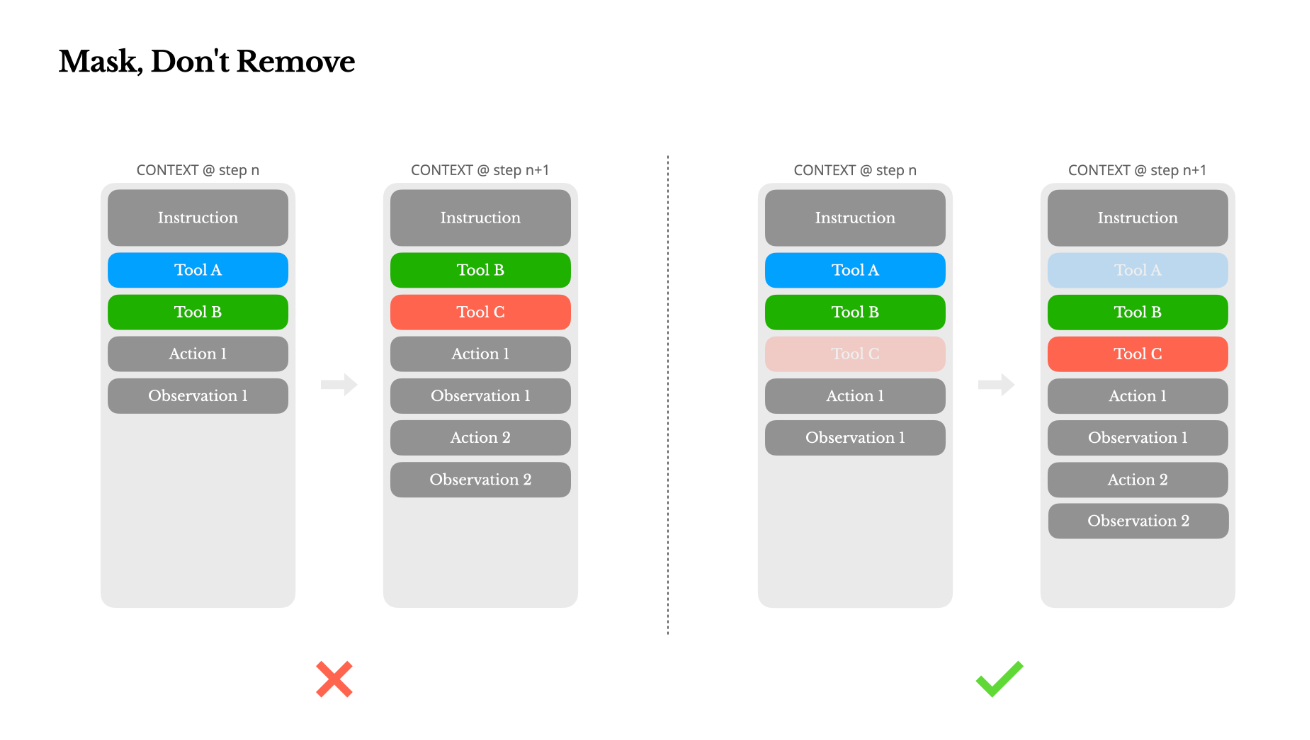
\includegraphics{images/image-0036.png}
\caption{掩蔽工具而不是从上下文移除工具}
\end{figure}

函数调用通常有三种模式：

自动：模型可以选择调用或不调用函数。通过仅预填充回复前缀实现：\textless\textbar im\_start\textbar\textgreater assistant

必需：模型必须调用函数，但选择不受约束。通过预填充到工具调用令牌实现：\textless\textbar im\_start\textbar\textgreater assistant

指定：模型必须从特定子集中调用函数。通过预填充到函数名称的开头实现：\textless\textbar im\_start\textbar\textgreater assistant\{``name'': ``browser\_''\}

\hypertarget{ux4e09ux4e0aux4e0bux6587ux7a97ux53e3-ux6587ux4ef6ux7cfbux7edfux5206ux5c42ux7ed3ux6784}{%
\subsection{三、``上下文窗口-文件系统''分层结构}\label{ux4e09ux4e0aux4e0bux6587ux7a97ux53e3-ux6587ux4ef6ux7cfbux7edfux5206ux5c42ux7ed3ux6784}}

上下文窗口有限，而信息的压缩是不可逆的。为此，我们可以只将重要信息留存在上下文窗口，其余则存储在文件系统中。模型学会按需写入和读取文件，不仅将文件系统用作存储，还用作结构化的外部记忆。

\begin{figure}[htbp]
\centering
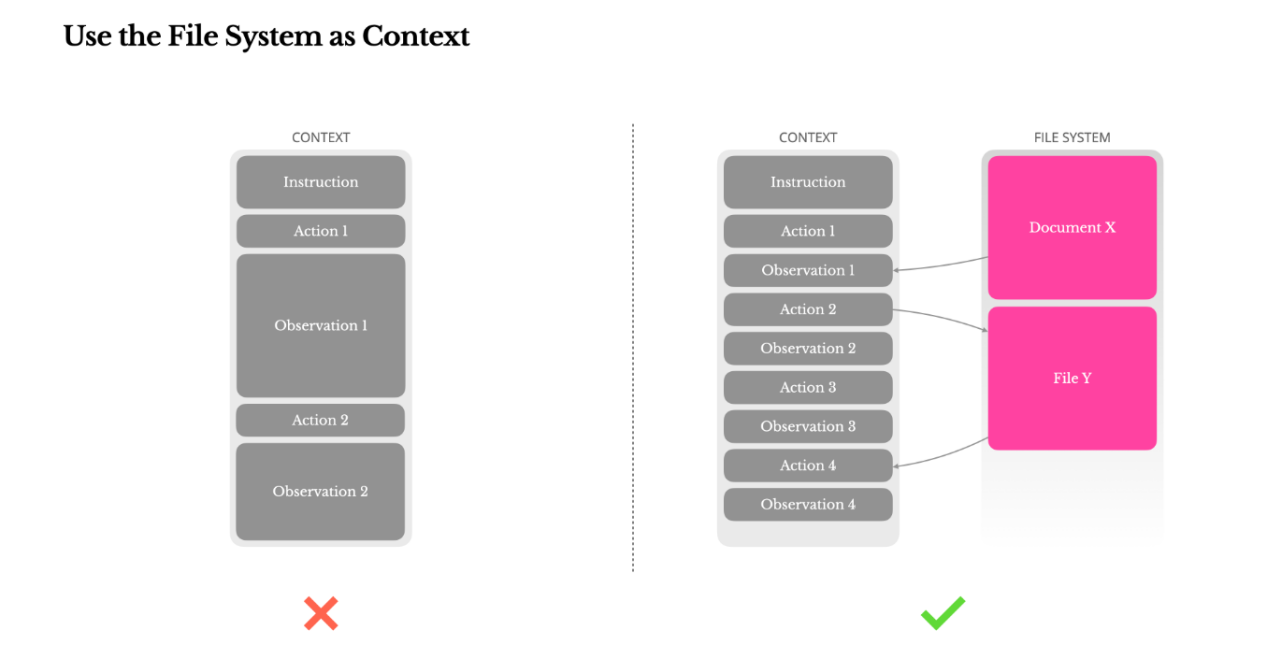
\includegraphics{images/image-0037.png}
\caption{将文件系统作为上下文}
\end{figure}

当上下文将满时，模型触发压缩（即在上下文最后加一条消息表示需要压缩）。对于工具调用结果，除了本轮会话以外，前面各轮会话的工具调用结果都会被压缩为指向文件系统中对应内容的索引。

\begin{figure}[htbp]
\centering
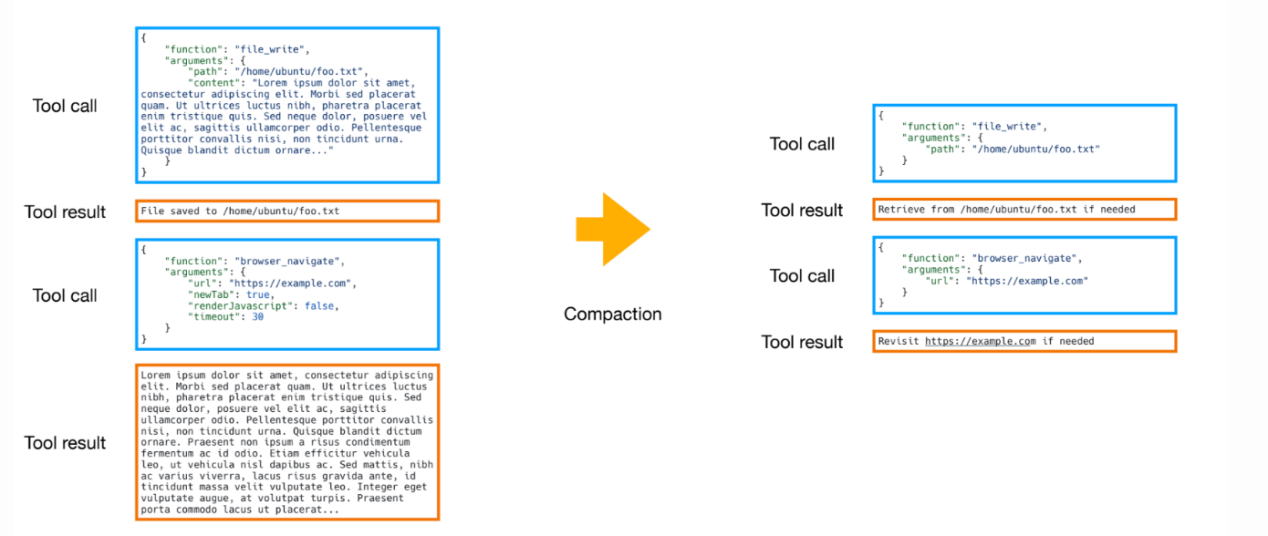
\includegraphics{images/image-0038.png}
\caption{将工具调用结果压缩为文件系统引用}
\end{figure}

\hypertarget{ux56dbux590dux8ff0ux76eeux6807}{%
\subsection{四、复述目标}\label{ux56dbux590dux8ff0ux76eeux6807}}

在处理复杂任务时，很多Agent会倾向于创建类似于todo.md的计划文件，并在任务进行过程中逐步更新它，勾选已完成的项目。这不仅是为了方便用户审阅，更重要的是，这是在操控注意力，通过将其目标复述到上下文的末尾的方式，避免模型在复杂任务后期偏离目标。

\begin{figure}[htbp]
\centering
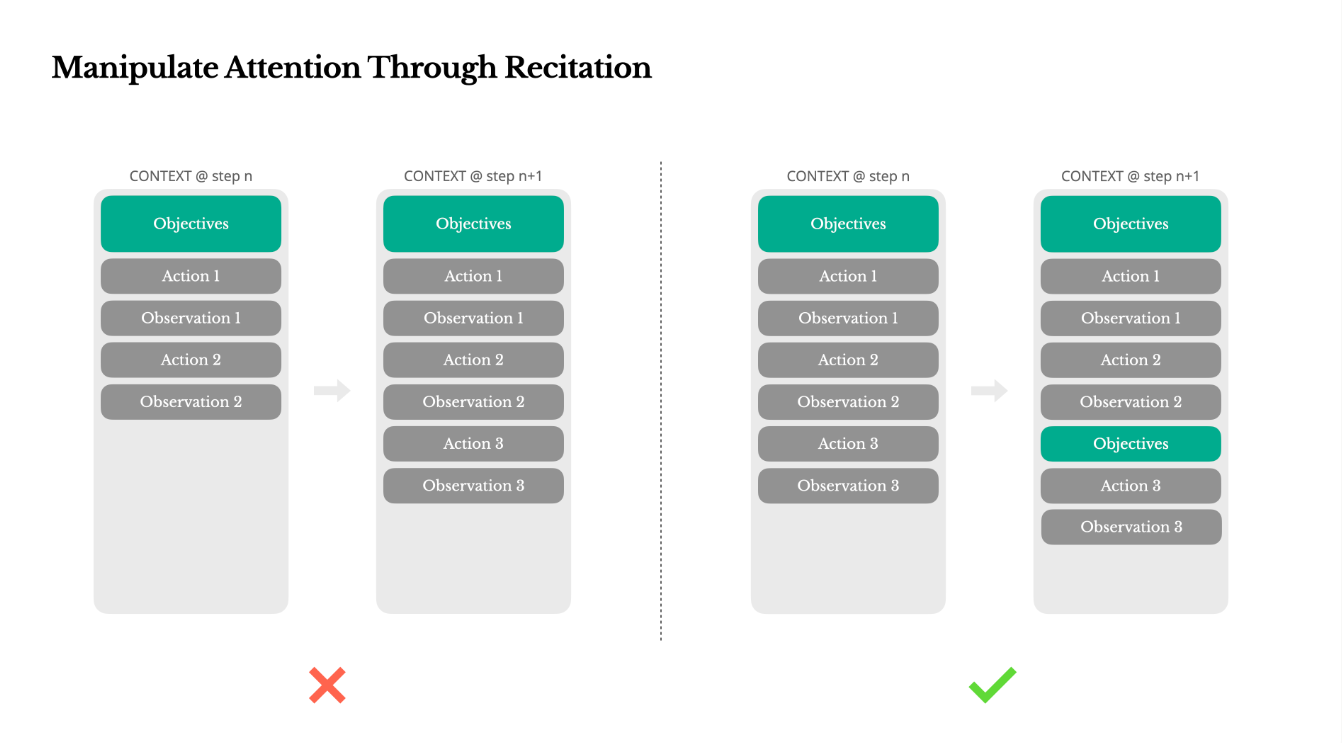
\includegraphics{images/image-0039.png}
\caption{通过复述目标操控注意力}
\end{figure}

\hypertarget{ux4e94ux4e0dux8981ux88abux5c11ux6837ux672cux793aux4f8bux6240ux56f0}{%
\subsection{五、不要被少样本示例所困}\label{ux4e94ux4e0dux8981ux88abux5c11ux6837ux672cux793aux4f8bux6240ux56f0}}

语言模型是优秀的模仿者；它们模仿上下文中的行为模式。如果上下文充满了类似的过去行动-观察对，模型将倾向于遵循该模式，即使这不再是最优的。这在涉及重复决策或行动的任务中可能很危险。例如，当审查20份简历时，代理通常会陷入一种节奏，即仅仅因为这是它在上下文中看到的，就重复与之类似的行动。这导致偏离、过度泛化，或有时产生幻觉。

解决方法是增加多样性，在行动和观察中引入少量的结构化变化，如不同的序列化模板、替代性措辞、顺序或格式上的微小噪音。这种受控的随机性有助于打破模式并调整模型的注意力。

\begin{figure}[htbp]
\centering
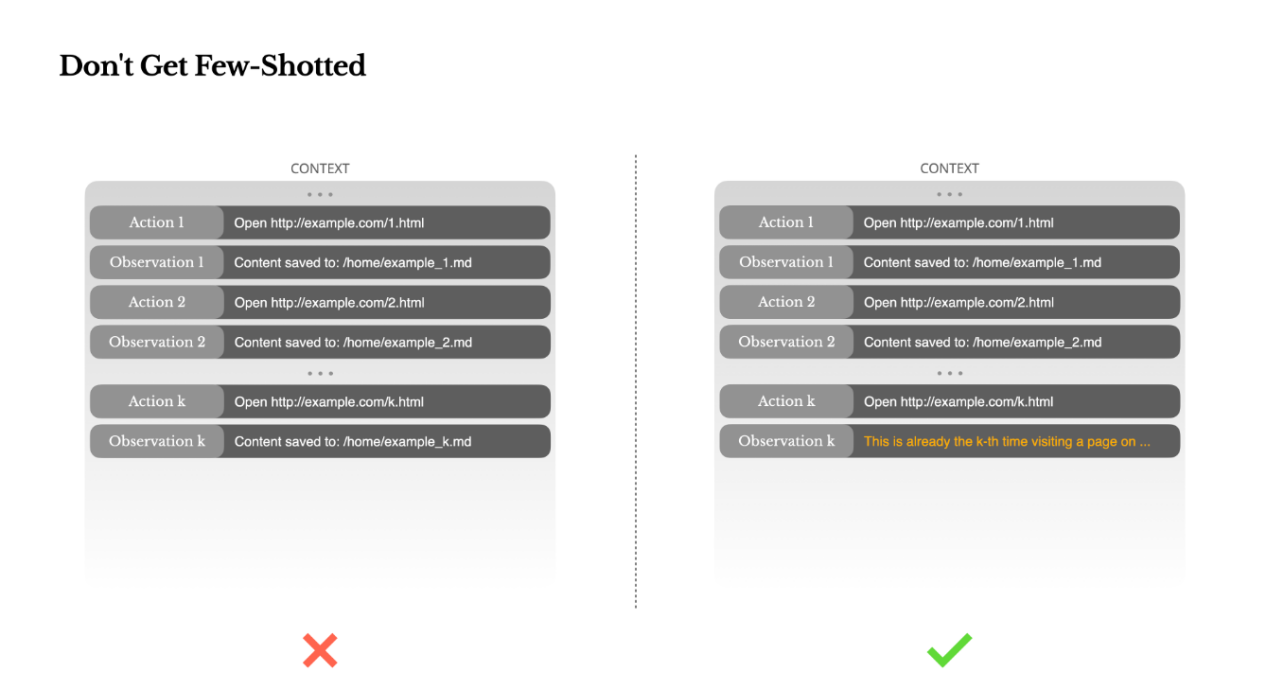
\includegraphics{images/image-0040.png}
\caption{避免少样本示例锁定行为模式}
\end{figure}

\hypertarget{ux516dux591aux667aux80fdux4f53ux7684ux4e0aux4e0bux6587ux9694ux79bb}{%
\subsection{六、多智能体的上下文隔离}\label{ux516dux591aux667aux80fdux4f53ux7684ux4e0aux4e0bux6587ux9694ux79bb}}

在多智能体系统中，主Agent和子Agent（如分别作为规划器和执行器）的上下文会存在一定隔离，如二者的system prompt和tools定义不同的。其余上下文可以不共享，但长上下文的复杂任务中仍建议共享。

不共享的范式：

\begin{figure}[htbp]
\centering
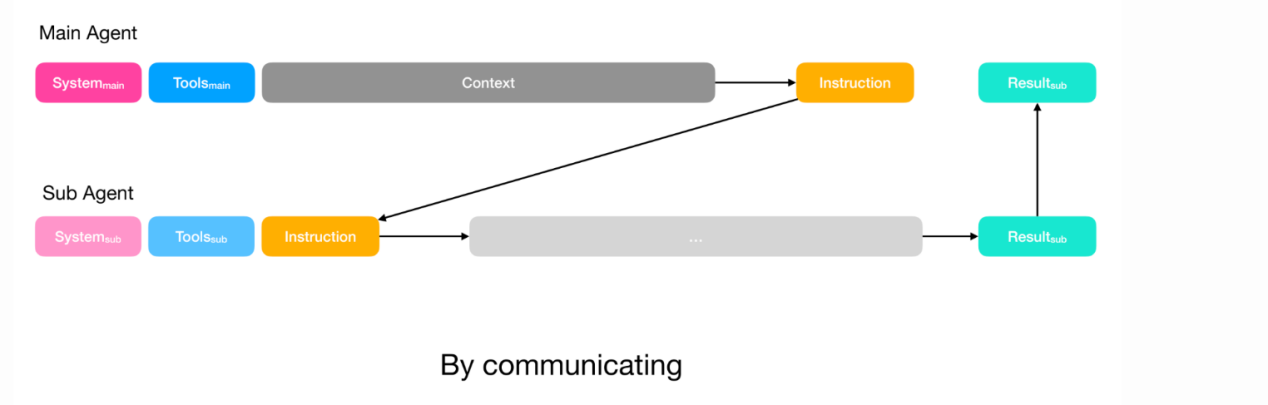
\includegraphics{images/image-0041.png}
\caption{主 Agent 与子 Agent 通过通信隔离上下文}
\end{figure}

部分共享的范式：（如主Agent作为规划者，与子Agent共享完整的上下文，子Agent仍拥有自己的动作空间（工具）和指令，但会获得规划者同样可访问的完整上下文。）

\begin{figure}[htbp]
\centering
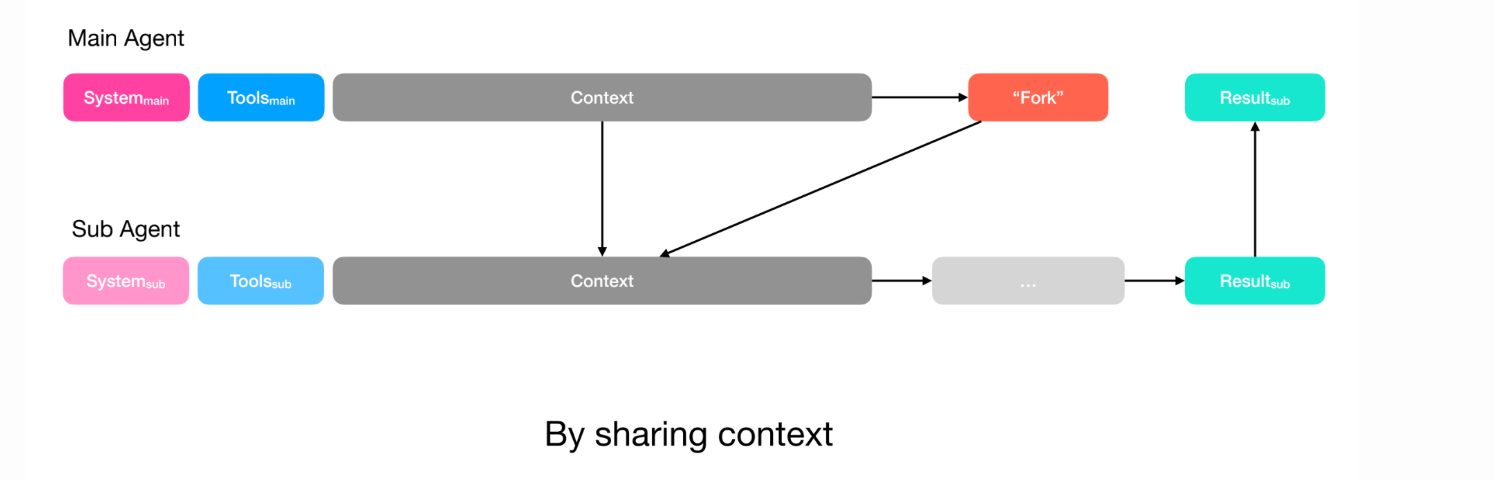
\includegraphics{images/image-0042.png}
\caption{主 Agent 与子 Agent 共享上下文}
\end{figure}

在这两种情况下，规划者都定义了子代理的输出模式。子代理有工具在返回结果前填充该模式，Manus 则使用约束解码确保输出符合定义模式。\texttt{submit\ results}

\hypertarget{ux53c2ux8003ux6587ux732e-134}{%
\subsection{参考文献}\label{ux53c2ux8003ux6587ux732e-134}}

\begin{itemize}
\tightlist
\item
  Martin, L. (2025). \href{https://rlancemartin.github.io/2025/10/15/manus/}{Context Engineering for Agents}.
\item
  Manus. (2025). \href{https://manus.im/zh-cn/blog/Context-Engineering-for-AI-Agents-Lessons-from-Building-Manus}{Context Engineering for AI Agents: Lessons from Building Manus}.
\end{itemize}

\clearpage

\hypertarget{ux57faux4e8eux6ce8ux610fux529bux5339ux914dux7684kvux538bux7f29ux8bbaux6587}{%
\section{基于注意力匹配的KV压缩（论文）}\label{ux57faux4e8eux6ce8ux610fux529bux5339ux914dux7684kvux538bux7f29ux8bbaux6587}}

\begin{quote}
本文是论文阅读笔记，内容代表对应论文方法或作者理解，不应直接视为领域共识或工程最佳实践。
\end{quote}

\hypertarget{ux4e00ux63d0ux51faux80ccux666f-3}{%
\subsection{一、提出背景}\label{ux4e00ux63d0ux51faux80ccux666f-3}}

在长上下文场景中，将长上下文总结为短文本虽然常用，但会丢失大量信息；在潜在空间训练紧凑KV缓存的方法（如Cartridges方法）能保持高性能，但需要昂贵的端到端梯度优化，耗时极长，通常需要数小时GPU算力才能压缩一个上下文。于是，我们希望不依赖于端到端的输出概率优化，而是直接优化紧凑的键和值，使其在每一个KV头上，对于每一个query，尽可能复现原始的``注意力输出''和``注意力质量（Attention Mass）''。

\hypertarget{ux4e8cux6838ux5fc3ux601dux60f3-3}{%
\subsection{二、核心思想}\label{ux4e8cux6838ux5fc3ux601dux60f3-3}}

该方法的核心思想是：不依赖于端到端的输出概率优化，而是直接优化紧凑的键和值，使其在每一个 KV 头上，尽可能复现原始的``注意力输出''和``注意力质量（Attention Mass）''。

假设原始上下文有 \(T\) 个 token，其键和值为 \(K,V \in \mathbb{R}^{T \times d}\)，我们要将其压缩为长度为 \(t\)（其中 \(t<T\)）的紧凑缓存 \(C_k,C_v \in \mathbb{R}^{t \times d}\)。为了补偿压缩后注意力总量的流失，作者引入了一个每个 token 标量偏差（Scalar Bias）\(\beta \in \mathbb{R}^{t}\)。

给定一组参考查询（Reference Queries）\(q \in \mathbb{R}^{1 \times d}\)，我们需要同时满足以下两个数学目标：

\begin{enumerate}
\def\labelenumi{\arabic{enumi}.}
\tightlist
\item
  匹配局部注意力输出（Local Attention Output）：
\end{enumerate}

\[
\frac{\exp(qK^\top)V}{\sum_{j=1}^{T}\exp(qK_j^\top)}
\approx
\frac{\exp(qC_k^\top+\beta)C_v}{\sum_{j=1}^{t}\exp(q(C_k)_j^\top+\beta_j)}
\]

这是为了对于 query，经过上下文聚合后输出的结果不变。

\begin{enumerate}
\def\labelenumi{\arabic{enumi}.}
\setcounter{enumi}{1}
\tightlist
\item
  匹配注意力质量（Attention Mass）：
\end{enumerate}

\[
\sum_{j=1}^{T}\exp(qK_j^\top)
\approx
\sum_{j=1}^{t}\exp(q(C_k)_j^\top+\beta_j)
\]

这是为了确保被压缩后的旧上下文，在未来遇到新输入的 token 时，依然能保持与原始完整上下文同等的``话语权''或``权重占比''。

传统的上下文压缩方法（如 Token 丢弃、KVzip 等）通常只是从 \(T\) 个 token 中挑出 \(t\) 个重要的 token 留下来（\(t<T\)）。

因为指数函数 \(\exp(x)\) 永远大于 0，所以保留 \(t\) 个 token 的 Mass 必然会系统性地小于原始 \(T\) 个 token 的 Mass：

\[
\sum_{j=1}^{t}\exp(q(C_k)_j^\top)
<
\sum_{j=1}^{T}\exp(qK_j^\top)
\]

当你用这种粗暴的压缩方法后，一旦系统追加了新的 token（\(K_{fixed}\)），由于压缩块的 Mass 变小了，它在上述加权混合公式中的占比就会骤降。模型会不成比例地把注意力过度集中在``新 token''上，从而在数学层面上被动地``遗忘''或``忽视''了被压缩的历史上下文。

一个通俗的类比：股东大会代表制。

\begin{itemize}
\tightlist
\item
  原始情况：公司有 1000 个小股东（原始 \(T\) 个 token），每人 1 票，总投票权（Attention Mass）为 1000。
\item
  传统压缩（丢弃法）：选出 50 个核心股东代表去开会，其他人不去。如果按人头算，旧股东阵营的总投票权骤降到 50。当有新投资人（new token）带着 100 票入场时，旧股东阵营的话语权会被彻底稀释。
\item
  匹配注意力质量（论文做法）：同样选出 50 个代表（挑选 \(C_k\)），但是赋予他们``代理投票权''（标量偏差 \(\beta\)），比如代表 A 身上背了 20 个人的票，代表 B 身上背了 30 个人的票。这样虽然人少了，但旧阵营的总票数依然是 1000（Mass 匹配）。当新投资人进来时，旧阵营的决策影响力（局部注意力输出）和话语权占比（混合权重）依然完美保持不变。
\end{itemize}

\hypertarget{ux4e09ux7b97ux6cd5ux6d41ux7a0b}{%
\subsection{三、算法流程}\label{ux4e09ux7b97ux6cd5ux6d41ux7a0b}}

共分3个步骤：采样参考查询（\(Q_{\mathrm{ref}}\)）；选择保留的键（\(C_k\)）并拟合偏差（\(\beta\)）；得到值（\(C_v\)）。

\hypertarget{ux4e00step1ux91c7ux6837ux53c2ux8003ux67e5ux8be2q_mathrmref}{%
\subsubsection{\texorpdfstring{（一）Step1：采样参考查询（\(Q_{\mathrm{ref}}\)）}{（一）Step1：采样参考查询（Q\_\{\textbackslash mathrm\{ref\}\}）}}\label{ux4e00step1ux91c7ux6837ux53c2ux8003ux67e5ux8be2q_mathrmref}}

对于不同的查询 \(Q\)，模型在用这些 \(Q\) 查询原文时，为了保证语法的连贯性、指代的准确性以及语义的连贯，会同时把注意力分散到历史中的多个关键 token 上。那些在不同 \(Q\) 下多次获得较高注意力分数的关键词，就是高价值的、需要保留的信息。我们无法预知未来的用户提问，也就不知道未来的 \(Q\) 分布，故我们希望诱导模型生成高质量的 \(Q\)。有以下两种方法：

\begin{enumerate}
\def\labelenumi{\arabic{enumi}.}
\tightlist
\item
  Repeat-prefill（重复预填充）
\end{enumerate}

它的具体做法是构造这样一个特殊的输入序列送给模型：

\begin{verbatim}
"[原始长文本 C] 接下来，请一字不差地重复前面的文本：[再次输入原始长文本 C]"
\end{verbatim}

内部重构时的``疯狂回看''：当模型在预填充（Prefill）阶段处理到第二个 \texttt{\{C\}} 时，为了准确预测下一个词，当前 token 的 \(Q\) 向量必须极度精准地去匹配第一个 \texttt{\{C\}} 中对应位置的 \(K\) 向量。这就好比你在抄写一段长文，你的眼睛（Query）会不断地、强烈地去回看原稿（Key）。

提取参考查询：这个``回看''过程中产生的 \(Q\) 向量，完美代表了``当模型真正需要从长上下文中精确提取细节时，它会发出怎样的查询请求''。

提取出来：在代码层面，我们只是在模型前向传播（Forward Pass）经过这些特定 token 时，把某些层注意力头里计算出的 \(Q\) 矩阵直接拷贝并保存下来。这些真实且高质量的 \(Q\) 就构成了我们的``参考查询集（\(Q_{ref}\)）''，作为后续压缩算法的``靶子''。

当大模型在输出``哪怕是一个完全`照抄'的词''时，它为了保证语法的连贯性、指代的准确性以及语义的连贯，其内部的 Query 向量会同时把注意力分散到历史中的多个关键节点上。

\begin{itemize}
\tightlist
\item
  举个例子：原文如果是``苹果公司在今天的发布会上，揭出了一部全新的手机。''
\item
  当模型在``重复''生成``手机''这个词时，它的 \(Q\) 向量不仅会去看原文末尾的``手机''，还会分配大量的注意力去看``苹果公司''、``库克''和``发布会''。因为模型需要这些上下文来确定当前语境。
\item
  结果就是：像``苹果公司''、``库克''这样的核心实体词（Key），会在模型重复整段话的过程中，被无数个后续生成的词的 \(Q\) 反复``回看''和依赖。
\end{itemize}

\begin{enumerate}
\def\labelenumi{\arabic{enumi}.}
\setcounter{enumi}{1}
\tightlist
\item
  Self-study（自学/自我提问）
\end{enumerate}

这是一种基于合成数据的方法。我们将原始上下文 \texttt{\{C\}} 喂给模型，并给它下一些指令（例如``总结关键事实''或``根据上下文提出 3 个问题''），让模型自己生成对话或问答。在模型``生成响应（Decoding）''的过程中，提取其注意力头产生的查询向量。这模拟了真实下游推理任务中查询向量的分布。

\hypertarget{ux4e8cstep2ux9009ux62e9ux4fddux7559ux7684ux952ec_kux5e76ux5229ux75282ux5f0fux62dfux5408ux504fux5deebeta}{%
\subsubsection{\texorpdfstring{（二）Step2：选择保留的键（\(C_k\)）并利用（2）式拟合偏差（\(\beta\)）}{（二）Step2：选择保留的键（C\_k）并利用（2）式拟合偏差（\textbackslash beta）}}\label{ux4e8cstep2ux9009ux62e9ux4fddux7559ux7684ux952ec_kux5e76ux5229ux75282ux5f0fux62dfux5408ux504fux5deebeta}}

只有一定数量的 token 会被保留，它们的键构成 \(C_k\)。这一步选择保留哪些 token（即保留哪些键）。有以下两种方法：

\begin{enumerate}
\def\labelenumi{\arabic{enumi}.}
\tightlist
\item
  保留最高注意力键并拟合偏差
\end{enumerate}

计算局部注意力分数：针对每一个参考查询 \(q_i\)，计算其在所有原始键 \(K\) 上的 Softmax 注意力分布：

\[
a_i = \mathrm{softmax}(q_i K^\top) \in \mathbb{R}^{1 \times n}
\]

跨查询聚合打分：对于第 \(j\) 个键，它在 \(n\) 个不同查询下会得到 \(n\) 个分数 \((a_{1,j}, a_{2,j}, \ldots, a_{n,j})\)。通过计算这些分数的均方根（Root Mean Square, RMS），得到该键的全局重要性得分 \(s_j\)。

排序与截断：根据 \(s_j\) 对所有原始键进行降序排列，直接提取 Top-\(t\) 个键构成 \(C_k\)。
在选择好一定数量键后，为保证注意力质量不变，根据（2）式，需要加上偏差。

我们的根本目标是让压缩后的缓存，在任意查询 \(q_i\) 下，其``注意力质量''等于原始缓存的质量 \(m_i\)：

\[
m_i = \sum_{j=1}^{T} \exp(q_i K_j^\top)
\]

为了用少量的 \(t\) 个键（\(C_k\)）凑出原本庞大的质量 \(m_i\)，作者为每个选中的键引入了一个待学习的标量偏差（Scalar Bias）\(\beta_j\)。近似等式变为：

\[
m_i \approx \sum_{j=1}^{t} \exp(q_i (C_k)_j^\top + \beta_j)
\]

根据指数函数的性质 \(\exp(A + B) = \exp(A)\exp(B)\)，我们可以将上式拆解为：

\[
m_i \approx \sum_{j=1}^{t} \exp(\beta_j) \cdot \exp(q_i (C_k)_j^\top)
\]

此时，我们定义一个新变量 \(w_j = \exp(\beta_j)\)。由于任何实数的指数都必定大于 0，所以这里的 \(w_j\) 隐含了一个严格的物理约束：它必须是非负的（\(w_j > 0\)，或放宽至 \(w_j \ge 0\)）。等式变形为：

\[
m_i \approx \sum_{j=1}^{t} w_j \exp(q_i (C_k)_j^\top)
\]

我们将所有参考查询上的方程联立，写成矩阵形式。令矩阵 \(A_{ij} = \exp(q_i (C_k)_j)\)，权重向量 \(w = [w_1,\ldots,w_t]^\top\)，目标向量为 \(m\)。上面的方程组就可以简洁地表示为：

\[
Aw \approx m
\]

为了找到最能让等式成立的 \(w\)，我们最小化等式两边的几何距离（L2 范数），并带入前面推导出的非负约束。这就构成了经典的 NNLS 目标函数：

\[
\min_{w \ge 0}\|Aw - m\|_2^2
\]

\begin{itemize}
\tightlist
\item
  固定选好的 \(C_k\) 后，目标是求解权重向量 \(w\)（其中 \(w_j = \exp(\beta_j)\)）以匹配目标注意力质量 \(m\)。
\item
  这被转化为一个非负最小二乘（NNLS）优化问题：\(\min_{w \ge 0}\|Aw - m\|_2^2\)。
\item
  求解后取对数得到 \(\beta_j = \log(w_j)\)。直观上，\(w_j\) 代表保留下来的紧凑键``代理''了多少个原始键的注意力质量。
  但这种``选择得分最高的键''的策略的盲区在于忽视了键与键之间的相关性和重叠度。假设组建一支5人的篮球队，如果按``个体最高得分''来选，你可能会选出联盟里得分最高的5个中锋。他们每个人的绝对实力都极强（注意力分数极高），但把他们放在一个队里，由于位置和技能高度重合（信息冗余），球队根本无法运转。
\end{itemize}

在LLM的注意力机制中，如果原文中有两个表达相似概念的词，或者同一句话中的两个强关联 token，它们可能会在参考查询下同时获得极高的注意力分数。如果采用最高分数策略，算法会把这两个高度冗余的键都选进来，浪费了原本就极其稀缺的压缩容量。

\begin{enumerate}
\def\labelenumi{\arabic{enumi}.}
\setcounter{enumi}{1}
\tightlist
\item
  正交匹配追踪（Orthogonal Matching Pursuit, OMP）
\end{enumerate}

假设你想调配出一种极其复杂的特定颜色（目标注意力质量 \(m\)），但你手头有上万种基础颜料（原始的所有键 \(K\)），而由于成本限制，你最终只能挑出其中的 \(t\) 种来混合（预算 \(t\) 个紧凑键）。

OMP 采用的是一种贪心且不断自我修正的策略：

\begin{enumerate}
\def\labelenumi{\arabic{enumi}.}
\item
  贪心寻找：每次找都去盯着当前调出来的颜色和目标颜色之间的``色差''（残差）。在剩下的颜料里，挑出一种与这个``色差''最接近、最能弥补当前差距的颜料。
\item
  正交投影（重拟合）：每次挑入新颜料后，不能只管新加的，而是要把目前挑出来的所有颜料重新按比例混合一次（重新计算权重 \(w\)），以确保当前的混合方案在数学上是``最优解''（即残差与当前所选特征空间正交，误差最小）。
  这样，我们每次都取在语义上互补的键，就能尽可能覆盖全面的信息，不出现重复。
\item
  初始化阶段：计算原始上下文的``目标注意力质量向量'' \(m\)。设定初始残差 \(r = m\)（一开始差距最大），并将``已选键集合'' \(S\) 设为空集。
\item
  计算相关性（Compute Correlation）：遍历所有目前还没有被选中的原始键 \(j \notin S\)。计算当前残差 \(r\) 与该键对应的特征列 \(\Phi_{:,j}\) 之间的内积：
\end{enumerate}

\[
c_j = r^\top \Phi_{:,j}
\]

内积越大，说明这个键越能解释剩下的残差。

\begin{enumerate}
\def\labelenumi{\arabic{enumi}.}
\setcounter{enumi}{2}
\tightlist
\item
  贪心选择（Greedy Selection）：在所有未选的键中，找出相关性得分最高（也就是最对口）的那个键 \(j^\star\)，把它正式纳入已选集合 \(S\) 中：
\end{enumerate}

\[
S \leftarrow S \cup \{j^\star\}
\]

\begin{enumerate}
\def\labelenumi{\arabic{enumi}.}
\setcounter{enumi}{3}
\tightlist
\item
  重拟合权重（Refit Weights via NNLS）：这一步是 OMP 的灵魂。现在 \(S\) 里面有了新成员，我们需要对 \(S\) 中所有的键重新分配``代理权重''（标量偏差）。我们通过求解一个非负最小二乘（NNLS）问题，找到一组非负权重 \(w\)，使得它们组合起来最接近目标 \(m\)：
\end{enumerate}

\[
w \leftarrow \arg\min_{w \ge 0}\|\Phi_{:,S}w - m\|_2^2
\]

\begin{enumerate}
\def\labelenumi{\arabic{enumi}.}
\setcounter{enumi}{4}
\tightlist
\item
  更新残差（Update Residual）：用目标向量减去当前已拟合出的结果，计算出最新的残差：
\end{enumerate}

\[
r \leftarrow m - \Phi_{:,S}w
\]

这也可以视为从m向已有键构成的超平面作投影，找到残差。

\begin{enumerate}
\def\labelenumi{\arabic{enumi}.}
\setcounter{enumi}{5}
\tightlist
\item
  循环迭代：重复步骤 2 到步骤 5，每轮挑一个键，直到集合 \(S\) 中塞满了我们预设的 \(t\) 个键为止。
\end{enumerate}

\hypertarget{ux4e09step3ux5f97ux5230ux503ccv}{%
\subsubsection{（三）Step3：得到值（Cv）}\label{ux4e09step3ux5f97ux5230ux503ccv}}

现在 \(\beta\) 和 \(C_k\) 都确定了。由于加上了偏差 \(\beta\)，为保证注意力输出不变，根据（1）式，被选中的 token 的 \(C_v\) 不会等于其原来的 \(V\) 值。对于第 \(i\) 个测试查询，注意力输出 \(y_i\) 满足：

\[
y_i =
\frac{\exp(q_i K^\top)V}{\sum_{j=1}^{T}\exp(q_i K_j^\top)}
\]

在我们的压缩模型中，既然 \(C_k\) 和 \(\beta\) 已经固定，那么对于查询 \(q_i\)，它在压缩键上产生的归一化注意力权重也就彻底固定了。我们把它记为 \(x_i \in \mathbb{R}^{1 \times t}\)：

\[
x_i =
\frac{\exp(q_i C_k^\top + \beta)}{\sum_{j=1}^{t}\exp(q_i (C_k)_j^\top + \beta_j)}
\]

我们要寻找一个新的紧凑值矩阵 \(C_v \in \mathbb{R}^{t \times d}\)，使得它在权重 \(x_i\) 的加权下，输出的结果尽可能等于原始目标 \(y_i\)：

\[
x_i C_v \approx y_i
\]

那么，整个优化问题就变成了一个极其标准的普通线性回归（Ordinary Least Squares, OLS）：

\[
XC_v \approx Y
\]

我们要最小化它的 L2 误差：

\[
C_v = \arg\min_{C_v}\|XC_v - Y\|_2^2
\]

熟悉线性代数的话，可以直接写出它的解析解（正规方程）：

\[
C_v = (X^\top X)^{-1}X^\top Y
\]

\hypertarget{ux53c2ux8003ux6587ux732e-135}{%
\subsection{参考文献}\label{ux53c2ux8003ux6587ux732e-135}}

\begin{itemize}
\tightlist
\item
  Zweiger, A., Fu, X., Guo, H., \& Kim, Y. (2026). \href{https://arxiv.org/abs/2602.16284}{Fast KV Compaction via Attention Matching}. arXiv:2602.16284.
\end{itemize}

\clearpage


% 基于上下文的持续学习
\hypertarget{ux57faux4e8eux4e0aux4e0bux6587ux7684ux6301ux7eedux5b66ux4e60}{%
\chapter{基于上下文的持续学习}\label{ux57faux4e8eux4e0aux4e0bux6587ux7684ux6301ux7eedux5b66ux4e60}}

\hypertarget{ux6ce8ux610fux529bux673aux5236ux4e0eux68afux5ea6ux4e0bux964dux7684ux7b49ux4ef7ux6027}{%
\section{注意力机制与梯度下降的等价性}\label{ux6ce8ux610fux529bux673aux5236ux4e0eux68afux5ea6ux4e0bux964dux7684ux7b49ux4ef7ux6027}}

注意力模块Transformer的Attention层（包含残差流在内）整体上可以被看作是一种回归问题的梯度下降优化。

\hypertarget{ux4e00ux7ebfux6027ux6ce8ux610fux529bux7684ux8868ux8fbeux5f0f}{%
\subsection{一、线性注意力的表达式}\label{ux4e00ux7ebfux6027ux6ce8ux610fux529bux7684ux8868ux8fbeux5f0f}}

对于一组token（模型输入序列）\(\{e_1,\ldots,e_n\}\) 和 query（test）token \(e_{\mathrm{test}}\)，经过去除Softmax的注意力层（即线性注意力层，后面会探讨加上Softmax的情形）后，注意力的表达式为：

\[
\mathrm{Output}_{\mathrm{test}}=e_{\mathrm{test}}+PVK^\top q_{\mathrm{test}}
\tag{1}
\]

其中输出加上自身是因为残差连接；\(P\) 为输出投影矩阵。若我们将 \(V\) 视为 \((v_1,\ldots,v_t)\)，\(K\) 视为 \((k_1,\ldots,k_t)\)，则 \(VK^\top=\sum_i v_i k_i^\top\)，即：

\[
\mathrm{Output}_{\mathrm{test}}=e_{\mathrm{test}}+P\sum_i v_i k_i^\top q_{\mathrm{test}}
\tag{2}
\]

用类似RNN的方式表述即为：

\[
S_t=S_{t-1}+v_t k_t^\top
\]

\[
\mathrm{Output}_t=\mathrm{input}_t+PS_tq_t
\]

上式意味着，我们利用隐状态矩阵 \(S\) 构建了一个从 \(K\) 到 \(V\) 的映射，并获取在输入 \(q_t\) 时的输出，作为残差相加。忽略投影 \(P\)，这里的 \(V\) 实质上拟合的是``输出与输入之间的残差''。

\hypertarget{ux4e8cux6784ux9020ux7ebfux6027ux6a21ux578bux5e76ux8bc1ux660eux7b49ux4ef7ux6027}{%
\subsection{二、构造线性模型，并证明等价性}\label{ux4e8cux6784ux9020ux7ebfux6027ux6a21ux578bux5e76ux8bc1ux660eux7b49ux4ef7ux6027}}

假设我们正在进行 In-Context Learning（上下文学习），输入是一系列示例（演示数据）：\((x_1,y_1),(x_2,y_2),\ldots,(x_N,y_N)\)，以及一个新的查询输入 \(x_{\mathrm{test}}\)。

在 Transformer 中，每个 Token 会将输入特征和标签拼接在一起。我们定义上下文矩阵为：

\[
X=[x_1,x_2,\ldots,x_N],\qquad Y=[y_1,y_2,\ldots,y_N]
\]

\textbf{输入 Token：}假设将输入特征 \(x_i\) 和目标标签 \(y_i\) 拼接成一个列向量作为 token，即：

\[
e_i=\begin{pmatrix}x_i\\y_i\end{pmatrix}
\]

引入一个由权重矩阵 \(W\in\mathbb{R}^{N_y\times N_x}\) 参数化的参考线性模型 \(y(x)=Wx\)，以及一个包含输入样本 \(x_i\) 和标签 \(y_i\) 的训练数据集 \(D=\{(x_i,y_i)\}_{i=1}^{N}\)。学习的目标是最小化平方误差损失：

\[
L(W)=\frac{1}{2N}\sum_{i=1}^{N}\|Wx_i-y_i\|^2
\]

此时梯度下降的表达式（动态模型的更新方式）为：

\[
\Delta W=-\eta\nabla_W L(W)=-\frac{\eta}{N}\sum_{i=1}^{N}(Wx_i-y_i)x_i^\top
\]

（3）

这里的 \(Wx_i-y_i\) 和前面的 \(v_i\) 对应（而不是 \(y_i\) 和 \(v_i\) 对应），表示``按原始权重的输出（\(W_0x_i\)）和应输出的值（标签 \(y_i\)）的差距''；\(x_i\) 和前面的 \(k_i\) 对应；\(\eta/N\) 和前面的 \(P\) 对应。这也就意味着，每次输入一批样本，\(W\) 的权重就将变化 \(-P\sum_i v_i k_i^\top\)。

也就是说，这个权重矩阵 \(W\) 和前面讲的隐状态矩阵 \(S\) 不一样：\(W\) 是隐式的，表示 \(x\) 到最终 \(y\) 的映射；\(S\) 是显式的，表示 \(k\) 到 \(v\)（残差 \(Wx-y\)）的映射。\(\Delta W\) 和 \(S\) 成比例关系，\(W\) 的一次梯度下降相当于运用了 \(S\) 中存储的所有上下文token的梯度。\((W+\Delta W)x_{\mathrm{test}}\) 和 \(\mathrm{input}_t+S_tq_t\) 相对应。

对于测试token：

\[
e_{\mathrm{test}}=\begin{pmatrix}x_{\mathrm{test}}\\y_{\mathrm{init}}\end{pmatrix}
\]

我们初始化 \(y_{\mathrm{init}}\) 为 \(-W_0x_{\mathrm{test}}\)（后面会阐释为什么可以这么做）。通过构造 \(W_Q\)、\(W_K\)、\(W_V\) 矩阵，使得：

当前查询 token \(j\) 的 Query 向量：

\[
q_j=W_Q e_j=\begin{pmatrix}I_x&0\\0&0\end{pmatrix}\begin{pmatrix}x_j\\y_j\end{pmatrix}=\begin{pmatrix}x_j\\0\end{pmatrix}
\]

上下文 token \(i\) 的 Key 向量：

\[
k_i=W_K e_i=\begin{pmatrix}I_x&0\\0&0\end{pmatrix}\begin{pmatrix}x_i\\y_i\end{pmatrix}=\begin{pmatrix}x_i\\0\end{pmatrix}
\]

上下文 token \(i\) 的 Value 向量：

\[
v_i=W_V e_i=\begin{pmatrix}0&0\\W_0&-I_y\end{pmatrix}\begin{pmatrix}x_i\\y_i\end{pmatrix}=\begin{pmatrix}0\\W_0x_i-y_i\end{pmatrix}
\]

计算注意力：

\[
k_i^\top q_j=(x_i^\top,0)\begin{pmatrix}x_j\\0\end{pmatrix}=x_i^\top x_j
\]

\[
\sum_{i=1}^{N}v_i(k_i^\top q_j)=\sum_{i=1}^{N}\begin{pmatrix}0\\W_0x_i-y_i\end{pmatrix}(x_i^\top x_j)
\]

\[
PVK^\top q_j=\begin{pmatrix}\eta/N&0\end{pmatrix}\left(\sum_{i=1}^{N}(W_0x_i-y_i)x_i^\top x_j\right)
\]

这意味着对上下文中的 \(W_0x-y\) 进行``聚合''，可以视为得到的是 \(W_0x_{\mathrm{test}}-y_{\mathrm{test}}\)。我们想要的就是这个上下文聚合后得到的 \(y\) 值预测 \(y_{\mathrm{test}}=(W_0+\Delta W)x_{\mathrm{test}}\)，从而上式的下面部分就可以视为 \(W_0x_{\mathrm{test}}-y_{\mathrm{test}}=-\Delta W x_{\mathrm{test}}\)，也就是``原有输出-应然输出''。而这恰好和前面 \(\Delta W\) 的表达式对上了，因此：

\[
PVK^\top q_j=\begin{pmatrix}0\\-\Delta W x_j\end{pmatrix}
\]

这意味着对于test token，（1）式等价于：

这条式子的下面部分取相反数后，也就得到参数变换后（按 \(W_0+\Delta W\)）应该输出的值，即注意力模块的输出。

\hypertarget{ux4e09ux4e3aux4ec0ux4e484ux5f0fux6709ux8d1fux53f7ux660eux660e-y_mathrmtestwx_mathrmtestdelta-wx_mathrmtestux4e3aux4ec0ux4e48ux8fd9ux91ccux662fux51cfux53bb-delta-wx_mathrmtest}{%
\subsection{\texorpdfstring{三、为什么（4）式有负号，明明 \(y_{\mathrm{test}}=Wx_{\mathrm{test}}+\Delta Wx_{\mathrm{test}}\)，为什么这里是减去 \(\Delta Wx_{\mathrm{test}}\)？}{三、为什么（4）式有负号，明明 y\_\{\textbackslash mathrm\{test\}\}=Wx\_\{\textbackslash mathrm\{test\}\}+\textbackslash Delta Wx\_\{\textbackslash mathrm\{test\}\}，为什么这里是减去 \textbackslash Delta Wx\_\{\textbackslash mathrm\{test\}\}？}}\label{ux4e09ux4e3aux4ec0ux4e484ux5f0fux6709ux8d1fux53f7ux660eux660e-y_mathrmtestwx_mathrmtestdelta-wx_mathrmtestux4e3aux4ec0ux4e48ux8fd9ux91ccux662fux51cfux53bb-delta-wx_mathrmtest}}

这需要从多轮优化的角度分析。大模型中往往是多个注意力层串行处理数据，每一轮都把输入 \(x_{\mathrm{test}}\) 转变为输出 \(y_{\mathrm{test}}\)，它又作为新的 \(x_{\mathrm{test}}\) 输入下一个注意力层。这等价于对一个线性层进行多轮权重更新：刚开始输入 \(x_{\mathrm{test}}\) 时（权重 \(W_0\)）执行一次梯度下降（权重变为 \(W_0+\Delta W\)）并输出 \(y_{\mathrm{test}}\)，它又作为新的 \(x_{\mathrm{test}}\) 输入（其他 \(x_i\) 和 \(y_i\) 仍然取原来的值）此时权重已经变为 \(W_0+\Delta W\) 的模型，再结合上下文进行梯度下降、推理，以此类推。

以上模型确实是正确的等价，但我们知道，实际上Transformer的权重是不变的，因此我们试图将上述过程再做一个等价转换，让 \(W\) 不变，而上下文 \(y_i\) 可变，更符合Transformer本身静态结构对应的表达式（即（1）式）。除了计算输出值（这一点我们已经有办法了）外，``当下的 \(W\) 值''唯一的``用处''就是用于梯度下降，而由（3）式可知，线性层梯度下降的幅度和残差 \(Wx_i-y_i\) 成正比，因此 \(W\) 从 \(W_0\) 变为 \(W_0+\Delta W\)，等价于上下文token的标签 \(y_i\) 减少 \(\Delta Wx_i\)，这时Loss不变，残差不变，优化状态不变。因此，我们可以假设多个线性层串行组成模型，每个线性层的参数均为 \(W\)，改变上下文token的 \(y_i\)：

\[
y_i^{new}=y_i-\Delta W x_i
\]

下一层的 \(W\) 不改变，但是这时候上下文token里输入的不是原始的 \(y_i\)，而是 \(y_i^{new}\)，下一层再对 \(y_i^{new}\) 进行类似的处理，以此类推，就可以通过改变上下文来等价地实现改变权重。

但是这时候会出现一个问题：自注意力层不会区分上下文token和test token，我们为了保证残差不变，把 \(y_i\) 减去 \(\Delta Wx_i\)，但是 \(y_{\mathrm{test}}=W_0x_{\mathrm{test}}+\Delta Wx_{\mathrm{test}}\)，符号反了。于是我们把 \(y_{\mathrm{init}}\) 取为 \(-W_0x_{\mathrm{test}}\)，减去 \(\Delta Wx_{\mathrm{test}}\) 后恰好为 \(-W_0x_{\mathrm{test}}-\Delta Wx_{\mathrm{test}}\)，乘以一个对角线全 \(-1\) 的输出投影矩阵即可。

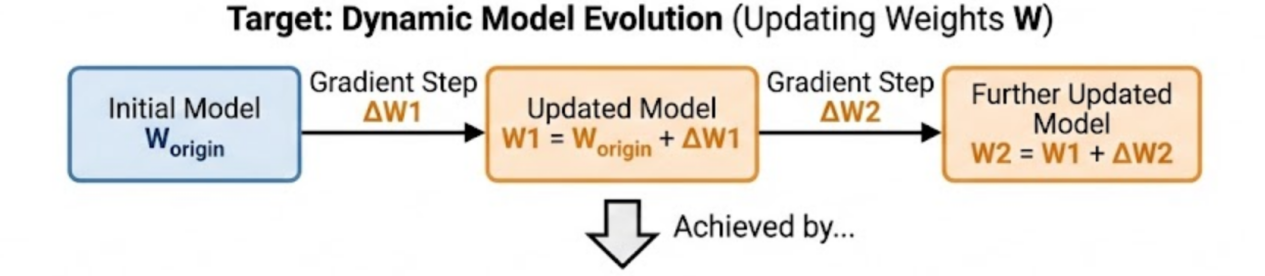
\includegraphics{images/image-0043.png}
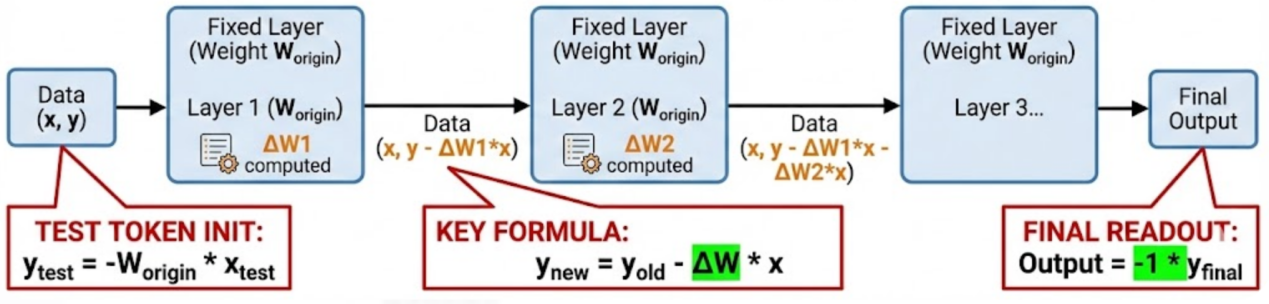
\includegraphics{images/image-0044.png}
- 穿过第 1 层注意力层（执行第 1 步梯度下降）：第 1 层根据当前的上下文计算出梯度增量 \(\Delta W_1\)。残差连接将其加上：

\[
y_{1,test}=y_{0,test}-\Delta W_1x_{\mathrm{test}}=-(W_0+\Delta W_1)x_{\mathrm{test}}
\]

\begin{itemize}
\tightlist
\item
  穿过第 2 层注意力层（执行第 2 步梯度下降）：第 2 层读取到 \(y_{1,test}\)，继续计算出新的梯度增量 \(\Delta W_2\)。残差连接再次将其加上：
\end{itemize}

\[
y_{2,test}=y_{1,test}-\Delta W_2x_{\mathrm{test}}=-(W_0+\Delta W_1+\Delta W_2)x_{\mathrm{test}}
\]

\begin{itemize}
\tightlist
\item
  穿过第 \(K\) 层注意力层（执行第 \(K\) 步梯度下降）：以此类推，经过 \(K\) 层后，测试 Token 的 \(y\) 值变成了：
\end{itemize}

\[
y_{K,test}=-W_0x_{\mathrm{test}}-\sum_{k=1}^{K}\Delta W_k x_{\mathrm{test}}
\]

\[
\hat{y}_{\mathrm{final}}=-y_{K,test}=W_0x_{\mathrm{test}}+\sum_{k=1}^{K}\Delta W_k x_{\mathrm{test}}
\]

这样，我们就把一个持续梯度下降的线性模型等价转化为了多个权重不变的线性层，数据在层间单向流动，每流过一个层，所有token（包括上下文token和test token）对应的 \(y\) 值都会减去 \(\Delta Wx\)，每一个这样的层就和Transformer中的每一个注意力层一一对应。值得注意的是，这样的 \(W_0\) 并非显式储存于Transformer的权重中，而是被隐式维护（虽然它也是不变的）：在前面的推理中，我们构造过：

\[
W_V=\begin{pmatrix}0&0\\W_0&-I_y\end{pmatrix}
\]

也就是说这里它由 \(W_V\) 决定。

总结：标准Transformer 无法在内部凭空变出一个真正的权重矩阵W存起来，只能靠修改数据流（残差）来``模拟''梯度下降，为了在多层Transformer中保证优化状态一致性，才采用了这种``别扭''的方式。

\hypertarget{ux56dbux5927ux6a21ux578bux4e2dux7684ux5b9eux9645ux60c5ux51b5}{%
\subsection{四、大模型中的实际情况}\label{ux56dbux5927ux6a21ux578bux4e2dux7684ux5b9eux9645ux60c5ux51b5}}

\hypertarget{ux4e00ux642cux8fd0ux673aux5236ux548cux5f52ux7eb3ux5934}{%
\subsubsection{（一）``搬运''机制和归纳头}\label{ux4e00ux642cux8fd0ux673aux5236ux548cux5f52ux7eb3ux5934}}

前面，我们只是在理论上证明了``自注意力有能力做梯度下降''。我们假设每个上下文token都由输入特征和标签拼接而成，但显然现实世界中的文本往往不符合这一点，输入特征和标签一般会分布在不同token中以随机位置出现。当面对这种真实随机的序列时，Transformer的第一层（包括了Softmax）并没有直接去算梯度，而是学习到了一种数据预处理功能：对于每一个含有y的token，通过q和K的匹配分数，找到它对应的x所在的token（不一定在x旁边，也不一定只有一个token），把x``搬运''到y所在的token里，再经过后面的线性层``整理''把向量变成类似于前述命题所需的(xi,yi)拼接状态。

这个搬运机制，恰好与Anthropic 团队之前发现的、被认为对上下文学习至关重要的``归纳头''（Induction Heads）现象吻合。第一层做的是Induction Head的拷贝工作，为后面开始执行真正的梯度下降（也就是前面推导的逻辑）、学习上下文铺平道路。在这里，Softmax起到了至关重要的作用：``搬运''意味着当前位置的Token必须能够百分之百地把注意力集中在目标Token（有需要的对应x值）上，同时绝对无视序列中的其他所有Token，这只有``赢家通吃''的Softmax能做到，如果纯粹用线性，往往会把序列里所有Token的特征都搅拌在一起（糊成一团），无法通过排除其他token的干扰来提取出极其干净的、单一的x。

\hypertarget{ux4e8cy_mathrminit-ux53d6ux4e3a--w_0x_mathrmtest-ux7684ux5408ux7406ux6027}{%
\subsubsection{\texorpdfstring{（二）\(y_{\mathrm{init}}\) 取为 \(-W_0x_{\mathrm{test}}\) 的合理性}{（二）y\_\{\textbackslash mathrm\{init\}\} 取为 -W\_0x\_\{\textbackslash mathrm\{test\}\} 的合理性}}\label{ux4e8cy_mathrminit-ux53d6ux4e3a--w_0x_mathrmtest-ux7684ux5408ux7406ux6027}}

而那个把 \(y_{\mathrm{init}}\) 取为 \(-W_0x_{\mathrm{test}}\) 的构造操作，在实际训练Transformer的时候，实际上只要我们将注意力权重初始化为一个非常小的值，就可以近似认为 \(W_V=0\)，进而由前面的分析 \(W_0=0\)，\(-W_0x_{\mathrm{test}}=0\)，而真实模型的第一层（归纳头）也会学习到主动把 \(y_{\mathrm{init}}\) 变换为接近0的值，在遇到test token时初始预测值就是0，随后通过层层残差连接去累加算出的梯度。

另外值得注意的是，这种模式往往只在部分层、（多头注意力的）部分头出现，后面也会阐述原因。

\hypertarget{ux4e09ux5173ux4e8e-y_mathrminit-ux4e0dux53c2ux4e0e-delta-w-ux7684ux8ba1ux7b97}{%
\subsubsection{\texorpdfstring{（三）关于 \(y_{\mathrm{init}}\) 不参与 \(\Delta W\) 的计算}{（三）关于 y\_\{\textbackslash mathrm\{init\}\} 不参与 \textbackslash Delta W 的计算}}\label{ux4e09ux5173ux4e8e-y_mathrminit-ux4e0dux53c2ux4e0e-delta-w-ux7684ux8ba1ux7b97}}

在上下文学习中，输入序列的形式为：

\[
\mathrm{Input}=[(x_1,y_1),(x_2,y_2),\ldots,(x_N,y_N),(x_{\mathrm{test}},y_{\mathrm{init}})]
\]

我们在上下文（准确地说是test token的前文）中通过梯度下降学习一个线性回归模型，再用这个模型预测 \(x_{\mathrm{test}}\) 对应的 \(y\) 值。显然，\(y_{\mathrm{init}}\) 不应该混入训练这个线性回归模型的数据，但自注意力层仍会``一视同仁''地将其纳入 \(\Delta W\) 的计算。

一种处理方法是掩码，把注意力权重矩阵对角线上的值全部设为负无穷。这将会导致训练时注意力矩阵从``下三角矩阵''变成``空心下三角矩阵''，导致为常规``下三角矩阵''设计的高度优化的Flash Attention等算子失效。

但事实上往往无需这样操作，因为根据之前的推导：

\[
V_t = W_0 x_t - y_t
\]

由前面的分析，\(-W_0x_{\mathrm{test}}=0\)，而真实模型的第一层（归纳头）也会学习到主动把 \(y_{\mathrm{init}}\) 变换为接近0的值，也就意味着此时 \(V_{\mathrm{test}}=0\)。这样，即便注意力权重没有被强制归零，它乘以的值 \(V_{\mathrm{test}}=0\)，也不会被累加到结果中，不会影响 \(\Delta W\) 的计算。

当然，真实的大模型中，显然不可能让所有test token的Value直接设为0，丢弃test token自身的信息。大模型有极其庞大的特征维度（子空间）和复杂的多头/多层分工机制，只有一部分层、一部分头是按这里所述运行的，以实现上下文学习功能；其他层、其他头中，test token的Value仍然会参与聚合，实现该token的语义处理等其他功能。真实模型不是全局丢弃了 Test Token 的 Value，而是把``提取语义''和``计算误差梯度''分给不同的注意力头去并行处理了。

值得一提的是，模型中的Attention Sink现象可能也有着类似的机制：

Transformer 每一层的公式是：输出 = 输入 + 注意力计算结果。

在深层网络中（比如 100 层的模型），很多时候，某几层可能觉得当前的特征（输入）已经足够完美了，不需要再从上下文中补充任何额外信息。此时，最理想的情况就是什么都不做，让特征顺着残差主干道原封不动地流到下一层。也就是说，模型希望：注意力计算结果 = 0，从而实现输出 = 输入 + 0。

但是，注意力机制里有一个极其霸道的数学公式：Softmax。Softmax 要求：所有 Token 的注意力权重加起来，必须 100\% 等于 1.0。

既然被逼着必须把 100\% 的注意力分配出去，而自己又不想改变特征，大模型（比如 Llama、GPT）在漫长的预训练中，自己``顿悟''出了一个绝招：

\begin{enumerate}
\def\labelenumi{\arabic{enumi}.}
\tightlist
\item
  找一个替罪羊（Sink Token）：模型通常会选中序列的第一个 Token（比如 \texttt{\textless{}s\textgreater{}}）或者第一个标点符号。
\item
  把它的 Value 变成 0：模型在训练参数时，偷偷把提取这个替罪羊 Value 的权重矩阵学成一种特殊状态，使得这个替罪羊的 \(V_{sink} \approx 0\)。
\item
  倾泻无用的注意力：当模型在某一层``不想关注任何上下文''时，它就强行把高达 99\% 的注意力分数（Attention Score）打给这个替罪羊。
\end{enumerate}

见证奇迹的时刻到了：这 99\% 的注意力权重乘上替罪羊的 \(V_{sink}\)：

\[
0.99 \times 0 = 0
\]

于是，整个注意力分支的计算结果变成了 0。输出 = 输入 + 0。模型成功地在满足 Softmax 苛刻要求的同时，完美地什么也没做，保持了特征的纯洁。

\hypertarget{ux56dbux771fux5b9eux8fd0ux884cux4e2dux54eaux4e9btokenux7684vux4f1aux88abux7f6eux4e3aux96f6}{%
\subsubsection{（四）真实运行中，哪些token的V会被置为零？}\label{ux56dbux771fux5b9eux8fd0ux884cux4e2dux54eaux4e9btokenux7684vux4f1aux88abux7f6eux4e3aux96f6}}

在真实的自回归序列中，输入不是拼好的 \((x,y)\)，而是每个 \(x\) 和 \(y\) 都分布在不同 token 中，如一个交替序列：\(x_1,y_1,x_2,y_2,\ldots,x_{19},y_{19},x_{20}\)。

当我们要生成 \(y_{19}\) 时（这时 \(y_{19}\) 还没有产生，被初始化为 \(0\)；test token 为 \(x_{19}\)）：

\begin{itemize}
\tightlist
\item
  浅层网络处理：因为这是新输入的 token，它还没有对应的 \(y_{19}\)。它的隐藏层状态只能是 \((x_{19},0)\)。
\item
  深层网络（梯度下降层）：深层网络提取它的 Value 向量。根据公式 \(V = W_0x - y\)，此时 \(V_{19}=W_0x_{19}-0 \approx 0\)。
\item
  结果：它完美地扮演了 Test Token，带着 \(V_{19}=0\) 去和前面的 KV Cache 算注意力，输出预测结果 \(\hat{y}_{19}\)。
\item
  物理沉淀：第 19 位的 KV Cache 被永久固化，其深度层的 \(V\) 永远是 0。
\end{itemize}

此时梯度下降用的是 \((x_1,y_1),(x_2,y_2),\ldots,(x_{18},y_{18})\)。\(x_{19}\) token 的 \(V\) 于是在KV Cache中被固化为 \(0\)。

注意：这里的深层网络不是最终的输出层，只是部分隐藏层的部分头。最终输出层的Value向量并不是0，无需担心信息损失。

当我们要生成 \(x_{20}\) 时（test token 为 \(y_{19}\)）：

\begin{itemize}
\tightlist
\item
  浅层网络处理（复制机制启动）：大模型的第 1 层（通常是 Softmax 归纳头）具有强大的时序视野。当它处理处于第 20 位的 \(y_{19}\) 时，它会向回看一眼第 19 位的 \(x_{19}\)，并把 \(x_{19}\) 的特征复制到自己的隐藏层状态中。
\item
  深层网络（梯度下降层）：当数据流到深层时，第 20 位的隐藏状态已经不再是单薄的 \(y_{19}\)，而是被浅层网络组装成了完整的上下文对 \((x_{19},y_{19})\)。
\item
  根据公式，深层网络在计算第 20 位的 Value 向量时：
\end{itemize}

\[
V_{20} = W_0x_{19} - y_{19} \ne 0
\]

\begin{itemize}
\tightlist
\item
  物理沉淀：第 20 位的 KV Cache 被固化，其深度层包含了一个非零的 \(V_{20}\)。
\end{itemize}

此时梯度下降用的还是 \((x_1,y_1),(x_2,y_2),\ldots,(x_{18},y_{18})\)。（不能包括 \((x_{19},y_{19})\)，因为这是 test token）

\(V_{y_{19}}=W_0x_{19}-y_{19}\ne 0\)。这一次计算后，KV Cache包含了一个非零的 \(V_{y_{19}}\)。

当我们要生成 \(y_{20}\) 时（test token 为 \(x_{20}\)）：

\(x_{20}\) 作为Query去遍历过去的KV Cache。

此时梯度下降用的是 \((x_1,y_1),(x_2,y_2),\ldots,(x_{18},y_{18}),(x_{19},y_{19})\)。

对于 \(x_{19}\)，它的 \(V_{19}=0\)，乘法结果为 \(0\)，直接被无视；对于 \(y_{19}\)，它的 \(V_{y_{19}}=W_0x_{19}-y_{19}\ne 0\)，提供了第 19 个样本的梯度信息。

\hypertarget{ux4e94transformerux5185ux90e8ux53eaux662fux6734ux7d20ux7684ux68afux5ea6ux4e0bux964dux5417}{%
\subsubsection{（五）Transformer内部只是朴素的梯度下降吗？}\label{ux4e94transformerux5185ux90e8ux53eaux662fux6734ux7d20ux7684ux68afux5ea6ux4e0bux964dux5417}}

部分后续研究指出，给Transformer喂了条件数极差的数据（特征矩阵极度不平衡）的情况下，其性能远优于普通的梯度下降。根据对中间层输出的分析，Transformer可能在内部自动收敛成了一个类似于迭代牛顿法的收敛轨迹，从而能在极短的Few-shot样本下瞬间学会新任务。

\hypertarget{ux4e94ux542bsoftmaxux7684ux60c5ux5f62}{%
\subsection{五、含Softmax的情形}\label{ux4e94ux542bsoftmaxux7684ux60c5ux5f62}}

\hypertarget{ux4e00ux5355ux5934softmaxux7684ux56f0ux5883ux5f15ux5165ux7ebfux6027ux504fux79fb}{%
\subsubsection{（一）单头Softmax的困境：引入线性偏移}\label{ux4e00ux5355ux5934softmaxux7684ux56f0ux5883ux5f15ux5165ux7ebfux6027ux504fux79fb}}

单层、单头的Softmax自注意力层无法完全匹配普通梯度下降的性能。其根本原因在于，Softmax的指数运算和归一化分母会在矩阵乘法中产生一个附加的误差项。这可以通过一阶泰勒展开近似说明。

在自注意力机制中，Softmax 函数作用于注意力分数（即 Query 和 Key 的内积）。对于当前的查询 Token \(x_j\) 和第 \(i\) 个上下文 Token \(x_i\)，未归一化的注意力分数为：

\[
z_i = k_i^T q_j = x_i^T W_{KQ}x_j
\]

将包含所有 \(N\) 个上下文 Token 的分数代入 Softmax 函数，第 \(i\) 个位置的输出为：

\[
\mathrm{softmax}(z)_i = \frac{e^{z_i}}{\sum_{k=1}^{N} e^{z_k}}
\]

根据高等数学中的一阶泰勒展开公式，当 \(z \to 0\) 时，指数函数可以近似为：

\[
e^z \approx 1 + z
\]

将这个近似代入 Softmax 的分子和分母中：

\begin{itemize}
\tightlist
\item
  分子：
\end{itemize}

\[
e^{x_i^T W_{KQ}x_j} \approx 1 + x_i^T W_{KQ}x_j
\]

\begin{itemize}
\tightlist
\item
  分母：
\end{itemize}

\[
\sum_{k=1}^{N} e^{x_k^T W_{KQ}x_j} \approx \sum_{k=1}^{N}(1+x_k^T W_{KQ}x_j)
\]

将所有 \(N\) 个 Token 的分子写成一个列向量：

\[
\begin{pmatrix}
1+x_1^T W_{KQ}x_j \\
\vdots \\
1+x_N^T W_{KQ}x_j
\end{pmatrix}
=
\mathbf{1}+
\begin{pmatrix}
x_1^T W_{KQ}x_j \\
\vdots \\
x_N^T W_{KQ}x_j
\end{pmatrix}
= \mathbf{1}+K^Tq_j
\]

其中 \(\mathbf{1}\) 是一个全为 1 的列向量。令分母的和为标量 \(S\)。那么 Softmax 的输出向量可以写为：

\[
\mathrm{softmax}(K^Tq_j) \approx \frac{1}{S}(\mathbf{1}+K^Tq_j)
= \frac{1}{S}K^Tq_j+\frac{1}{S}\mathbf{1}
\]

因此有：

\[
\mathrm{softmax}(K^Tq_j) \propto K^Tq_j+\mathbf{1}
\]

物理含义：这个 \(\epsilon\) 是一个常数偏移量（Linear Offset）。它意味着，即使某些 Token 和当前 Query 毫无关系（内积 \(x_i^TW_{KQ}x_j=0\)），Softmax 依然会强制分配给它们一个基础的权重（即 \(\frac{1}{S}\)）。这种``强制均分''的特性，污染了原本纯净的梯度方向，导致单头 Softmax 注意力无法完美执行梯度下降。
即便对于内积为负数的token（对应可能是数学推导中的错误方向），权重也会变成正值。这显然不合理。

\hypertarget{ux4e8cux591aux5934softmaxux5982ux4f55ux89e3ux51b3ux8fd9ux4e00ux95eeux9898}{%
\subsubsection{（二）多头Softmax如何解决这一问题}\label{ux4e8cux591aux5934softmaxux5982ux4f55ux89e3ux51b3ux8fd9ux4e00ux95eeux9898}}

前面提过，由于Softmax对于归纳头起着不可或缺的作用，我们无法通过直接去掉Softmax的方法来增强上下文学习能力。但既然偏移量1（即epsilon）为常数，那么多头Softmax可以通过不同头之间相减抵消来实现：

假设模型学习到了两个注意力头，并且在最后的输出投影层（Projection Layer）中，它将这两个头的权重学成了符号相反的形式，即使得 \(P_1V_1 \approx -P_2V_2\)。为了简化表达，论文假设这两个头提取误差的矩阵 \(PV\) 相同（或被网络调整到一致），但在内部的注意力特征矩阵 \(W_{KQ}\) 上学到了不同的特征空间。

我们将这两个头的注意力计算结果相减：

\[
\mathrm{Output} \approx PV \cdot \mathrm{softmax}(K_1^Tq_{1,j}) - PV \cdot \mathrm{softmax}(K_2^Tq_{2,j})
\]

将我们在第一部分得到的泰勒近似列向量代入上式（这里论文做了一个合理假设，即两个头经过 Softmax 的分母常数 \(S\) 近似相等，并将其吸收到 \(PV\) 中）：

\[
\mathrm{Output} \approx PV \left[
\begin{pmatrix}
1+x_1^TW_{1,KQ}x_j \\
\vdots
\end{pmatrix}
-
\begin{pmatrix}
1+x_1^TW_{2,KQ}x_j \\
\vdots
\end{pmatrix}
\right]
\]

接下来进行极其简单的线性代数运算，将对应行的元素相减。对于第 \(i\) 行：

\[
\begin{aligned}
(1+x_i^TW_{1,KQ}x_j)-(1+x_i^TW_{2,KQ}x_j)
&= 1-1+x_i^TW_{1,KQ}x_j-x_i^TW_{2,KQ}x_j \\
&= x_i^T(W_{1,KQ}-W_{2,KQ})x_j
\end{aligned}
\]

看，常数项 1（即那个讨厌的 \(\epsilon\) 偏移量）在减法中完美归零了。

\hypertarget{ux516dux4e3aux4ec0ux4e48transformerux4f5cux4e3aux4e00ux79cdux4e8bux5b9eux4e0aux7684ux5143ux5b66ux4e60ux7b97ux6cd5ux4ecdux4e0dux80fdux5f88ux597dux5730ux5e94ux5bf9oodux95eeux9898}{%
\subsection{六、为什么Transformer作为一种事实上的元学习算法，仍不能很好地应对OOD问题？}\label{ux516dux4e3aux4ec0ux4e48transformerux4f5cux4e3aux4e00ux79cdux4e8bux5b9eux4e0aux7684ux5143ux5b66ux4e60ux7b97ux6cd5ux4ecdux4e0dux80fdux5f88ux597dux5730ux5e94ux5bf9oodux95eeux9898}}

\hypertarget{ux4e00ux7279ux5f81ux63d0ux53d6ux7684ux56f0ux96be}{%
\subsubsection{（一）特征提取的困难}\label{ux4e00ux7279ux5f81ux63d0ux53d6ux7684ux56f0ux96be}}

我们在前面推导中的前提是，执行梯度下降的特征向量 \(x\)，是经过大模型的Embedding和MLP层投影后的深层表示。注意力层可以看成实时梯度下降，即视为元学习；但Embedding和MLP层并不是如此。如果遇到OOD问题（比如人类从未见过的数据模态），预训练阶段的MLP根本没有为这种数据建立特征坐标系。OOD数据在输入网络后，被MLP映射成了一堆毫无意义的噪声向量，无法顺利提取数据的特征，进而后续的注意力层在执行 \(y_{new}=y_{old}-\Delta Wx\) 时，算出的梯度也就是一团乱码。

\hypertarget{ux4e8cux68afux5ea6ux4e0bux964dux7684ux5c40ux9650ux6027}{%
\subsubsection{（二）梯度下降的局限性}\label{ux4e8cux68afux5ea6ux4e0bux964dux7684ux5c40ux9650ux6027}}

梯度下降算法本身的特点决定了，面对OOD任务时，大模型所谓的``学习''，并不是真正在寻找全局最优解，而是在它预训练时见过的``任务池''里，寻找一个和当前OOD任务最相似的替代品。它只能在已有的先验知识流形（Manifold）上插值，无法外推到一个全新的物理空间。

\hypertarget{ux4e09ux8ba1ux7b97ux6df1ux5ea6ux4e0dux8db3}{%
\subsubsection{（三）计算深度不足}\label{ux4e09ux8ba1ux7b97ux6df1ux5ea6ux4e0dux8db3}}

我们证明了：1层Transformer = 1步梯度下降。一个100层的模型，最多也只能执行几十步、上百步的有效梯度下降。而真正的OOD任务（比如从头训练一个视觉模型）往往需要几万、几十万步的梯度迭代才能收敛。大模型那极其有限的层数，根本无法提供足够的计算深度来完成OOD的参数拟合。

当然，随着RLVR带来的模型推理能力的提升，模型在完成一个任务（即上下文不清空）的情况下的KV Cache更新次数和有效计算深度大大增加。``组合型OOD''往往能被解决：如给一道全新的数学竞赛题，整体来看它是OOD的，但它可以把这个问题拆解，原子步骤（加减乘除、代数变换）都在它的先验特征空间内，RL训练出的思维链能通过千万步的内部梯度下降，把这些已知特征重新组合，最终攻克难题。但对于``绝对型OOD''，即输入的底层特征在模型的MLP中根本不存在映射的情况，该方法仍然无效。

\hypertarget{ux4e03ux4f18ux5316ux95eeux9898ux7684ux7b49ux4ef7ux6027}{%
\subsection{七、优化问题的等价性}\label{ux4e03ux4f18ux5316ux95eeux9898ux7684ux7b49ux4ef7ux6027}}

在神经心理学中，记忆是由输入引起的神经更新，而学习是获取有效和有用记忆的过程。我们遵循 Behrouz 等人的定义：

\textbf{定义 1（联想记忆）}：给定一组键（Keys）\(\mathcal{K}\subseteq\mathbb{R}^{d_k}\) 和值（Values）\(\mathcal{V}\subset\mathbb{R}^{d_v}\)，联想记忆是一个算子 \(\mathcal{M}:\mathcal{K}\to\mathcal{V}\)，用于映射这两组集合。为了从数据中学习这种映射，我们定义一个目标函数 \(\tilde{\mathcal{L}}(\cdot;\cdot)\) 来衡量映射的质量，\(\mathcal{M}\) 可以定义为：

\[
\mathcal{M}^*=\arg\min_{\mathcal{M}}\tilde{\mathcal{L}}(\mathcal{M}(\mathcal{K});\mathcal{V})
\tag{1}
\]

原理阐释与推导分析：

\begin{itemize}
\tightlist
\item
  核心思想：这里将``记忆''看作是一个函数 \(\mathcal{M}\)。传统的观点认为训练模型是调整参数，而这里的观点是：训练过程本身就是在一个函数空间中寻找最优解，使得这个函数能最好地把 Key 映射到 Value。
\item
  物理意义：方程 (1) 本质上是在说，最佳的记忆状态 \(\mathcal{M}^*\) 是那个能最小化预测误差的状态。在深度学习中，\(\mathcal{K}\) 通常是输入数据，\(\mathcal{V}\) 是标签或目标，\(\tilde{\mathcal{L}}\) 是损失函数。NL 的独特之处在于，它认为模型内部的每一个组件（甚至是优化器）都在解这样一个方程。
\end{itemize}

事实上，无论是Attention注意力模块的前向计算，还是传统意义上的``优化''，都可以视为这样一个``寻找最优函数''的过程。下面我们推导梯度下降法与其的等价性：

假设我们要用梯度下降法训练一个单层 MLP（参数为 \(W\)）。优化目标是：

\[
W^*=\arg\min_W\mathcal{L}(W;\mathcal{D}_{train})
\]

梯度下降的更新规则导致权重更新等价于：

\[
W_{t+1}=W_t-\eta_{t+1}\nabla_{W_t}\mathcal{L}(W_t;x_{t+1})
\]

这里 \(x_{t+1}\) 是在 \(t+1\) 时刻输入的一个批量训练数据。由于 \(y_{t+1}=W_tx_{t+1}\)，对 \(W_t\) 的梯度即为对 \(y_{t+1}\) 的梯度和 \(x_{t+1}\) 的积：

\[
W_{t+1}=W_t-\eta_{t+1}\nabla_{y_{t+1}}\mathcal{L}(W_t;x_{t+1})\otimes x_{t+1}
\tag{4}
\]

设 \(W_t\) 为此时模型的权重，\(x_{t+1}\) 为当前的输入，\(y_{t+1}=W_tx_{t+1}\) 为模型在当前权重的线性输出。我们把损失函数 \(\mathcal{L}(W_t;x_{t+1})\) 称为``惊讶程度''。这既是因为模型预测越正确，惊讶程度越低，也是因为交叉熵损失函数的信息论背景本来就是``惊讶度''。

我们定义``惊奇信号''为：

\[
u_{t+1}\triangleq \nabla_{y_{t+1}}\mathcal{L}(W_t;x_{t+1})
\]

其中：

\begin{itemize}
\tightlist
\item
  \(W_t\)：当前时刻的模型权重。
\item
  \(x_{t+1}\)：当前的输入数据。
\item
  \(y_{t+1}=W_tx_{t+1}\)：模型在当前权重的线性输出（假设是单层 MLP）。
\item
  \(\mathcal{L}\)：损失函数。
\end{itemize}

它可以理解为``Loss对神经网络输出层的指令''，即怎样调整网络的输出y，以使损失最小。

预测误差的直接体现：\(u_{t+1}\)（即 \(\nabla_y\mathcal{L}\)）直接衡量了模型当前的输出 \(y_{t+1}\) 和真实标签（或目标）之间的差距。

对于 \(t+1\) 时刻新输入的数据 \(x_{t+1}\)，如果我们只需要根据用已有数据训练出来的 \(W_t\)，就能将输入转化为正确标签 \(y_{t+1}\)，那么权重 \(W_t\) 已经是最优了，完全没有必要更新，\(u_{t+1}=0\)。反之，如果预测和 \(y_{t+1}\) 相差很大，惊讶程度就会很高，则意味着 \(W_t\) 需要较大的调整。

举一个例子：

\begin{enumerate}
\def\labelenumi{\arabic{enumi}.}
\tightlist
\item
  输入 \(x\)：``The sky is\ldots{}''
\item
  模型预测 \(y\)：``\ldots green''（绿色）
\item
  真实标签：``\ldots blue''（蓝色）
\end{enumerate}

在这个过程中：

\begin{itemize}
\tightlist
\item
  \(\mathcal{L}\)（惊讶程度）：模型发现真实是 Blue 而不是 Green，非常震惊。Loss 值很大（比如 5.0），这就是``惊讶程度''。
\item
  \(u_{t+1}\)（惊奇信号）：这个信号是一个向量，它告诉模型具体的误差信息：``Green 的概率太高了，要降低！''``Blue 的概率太低了，要升高！''这个向量 \(u_{t+1}\) 就是具体的``修正指令''。
\item
  Nested Learning 的记忆过程：模型会把这次经历存进 MLP：``当你下次看到 `The sky is\ldots{}'（\(x\)）时，记得要把那个叫 \(u\) 的修正指令调出来。''
\end{itemize}

这可以解释为什么神经网络（如MLP）可以作为记忆模块。训练前的神经网络里没有信息，给定一个输入x，它的输出y是一个噪声（先验为噪声分布）。而``训练''的过程，就可以视为告诉神经网络：``下次再遇到x，你的输出应该往u方向移动。''或者说，就是让它``记忆''输入与``碰到这个输入时，怎么（从先验的随机状态开始）改变自己的输出''之间的关系。

或者说，MLP的梯度下降更新本质是一个``压缩''过程，将当前输入数据及其对应``怎么修改输出''的信息``压缩''进权重中。模型通过持续进行在线梯度下降（Online Gradient Descent），实时地修改自己的神经网络权重，存储读过的数据片段的信息。

更进一步地说，惊奇信号的含义实际上是一种``反思''，即``根据当前神经网络输出与目标（标签）的差距来看，我的权重应该做怎样的改进''，并将反思写入权重，让模型实现在推理阶段的持续改进。

下面我们再以优化视角看这个问题：

同式 (4)，由于 \(y_{t+1}=Wx_{t+1}\) 是模型输出，我们可以令 \(u_{t+1}=\nabla_{y_{t+1}}\mathcal{L}(W_t;x_{t+1})\)，并将反向传播过程重新表述为寻找最优联想记忆的优化问题的解。也就是说，我们旨在找到映射输入 \(x_{t+1}\) 到其对应的 \(u_{t+1}\) 的最佳 \(W\)：

\[
W_{t+1}=\arg\min_W \langle Wx_{t+1},u_{t+1}\rangle+\frac{1}{2\eta_{t+1}}\lVert W-W_t\rVert_2^2
\tag{5}
\]

\[
=\arg\min_W\left\langle Wx_{t+1},\nabla_{y_{t+1}}\mathcal{L}(W_t;x_{t+1})\right\rangle+\frac{1}{2\eta_{t+1}}\lVert W-W_t\rVert_2^2
\tag{6}
\]

这条表达式的第一项是 \(Wx_{t+1}\)（输出）和 \(u_{t+1}\)（Loss 对输出的梯度）的点积相似度，\(W\) 的更新会让输出尽量沿着梯度的反方向；第二项是正则化项，避免权重更新过大。这一步将梯度下降公式逆向推导回了一个优化问题。

定义目标函数：

\[
J(W)=\left\langle Wx_{t+1},u_{t+1}\right\rangle+\frac{1}{2\eta_{t+1}}\lVert W-W_t\rVert_2^2
\]

步骤 1：对第一项求导。利用矩阵微分性质 \(\langle A,B\rangle=\mathrm{Tr}(A^\top B)\)，可得到：

\[
\frac{\partial}{\partial W}\left\langle Wx_{t+1},u_{t+1}\right\rangle
=\frac{\partial}{\partial W}\left(u_{t+1}^{\top}Wx_{t+1}\right)
=u_{t+1}x_{t+1}^{\top}
\]

注意：这里 \(u_{t+1}x_{t+1}^{\top}\) 正是外积形式的梯度项。

步骤 2：对第二项求导：

\[
\frac{\partial}{\partial W}\left(\frac{1}{2\eta_{t+1}}\lVert W-W_t\rVert_2^2\right)
=\frac{1}{2\eta_{t+1}}\cdot 2(W-W_t)
=\frac{1}{\eta_{t+1}}(W-W_t)
\]

步骤 3：求解使梯度为零的条件：

\[
\nabla_W J(W)=u_{t+1}x_{t+1}^{\top}+\frac{1}{\eta_{t+1}}(W-W_t)=0
\]

因此：

\[
W=W_t-\eta_{t+1}(u_{t+1}x_{t+1}^{\top})
\]

带动量的梯度下降也可以类似看待：

接下来，我们引入动量项。更新规则如下：

\[
W_{t+1}=W_t-m_{t+1}
\tag{7}
\]

\[
m_{t+1}=m_t+\eta_{t+1}\nabla_{W_t}\mathcal{L}(W_t;x_{t+1})
\tag{8}
\]

这里把 \(m_{t+1}\) 定义为从 \(W_t\) 中减去的更新量，因此它沿当前梯度方向累积；真正的参数更新仍然通过 \(W_{t+1}=W_t-m_{t+1}\) 沿负梯度方向前进。在方程 8 中，如果令 \(g_{t+1}=\nabla_{W_t}\mathcal{L}(W_t;x_{t+1})\)，那么方程 8 可以被重写为：

\[
m_{t+1}=\arg\min_m-\left\langle m,g_{t+1}\right\rangle
+\frac{1}{2\eta_{t+1}}\lVert m-m_t\rVert_2^2
\tag{10}
\]

分层结构：

\begin{itemize}
\tightlist
\item
  第 1 层（外层）：更新权重 \(W\)。它使用的是 \(m\) 的值。
\item
  第 2 层（内层）：更新动量 \(m\)。方程 (10) 表明，更新动量 \(m\) 的过程，实际上是在求解一个优化问题，目的是让 \(m\) 尽可能与当前的梯度方向一致（最大化点积或相似度），同时保持与上一步的 \(m_t\) 不会偏离太远（正则化项）。
\end{itemize}

结论：带有动量的梯度下降是一个双层嵌套优化过程。内层记忆负责``压缩''过去的梯度历史，外层利用这个压缩后的信息来更新模型。

事实上，前面的方程也可以被重写为这样的优化问题：

\[
m_{t+1}=\arg\min_m\left(
-\left\langle m,g_{t+1}\right\rangle
+\frac{1}{2\eta_{t+1}}\lVert m-m_t\rVert_2^2
\right)
\tag{10}
\]

这个优化问题描述了动量 \(m\) 是如何在每一步自我更新的。

项 A：趋势对齐（Alignment Term）

\[
-\left\langle m,\nabla_W\mathcal{L}\right\rangle
\]

\begin{itemize}
\tightlist
\item
  数学含义：这是两个向量的内积的负数。要最小化这个负值，就等于要最大化它们的正内积。
\item
  物理意义：这要求新的动量 \(m\) 的方向，必须尽可能地与当前的梯度方向 \(\nabla_W\mathcal{L}\) 保持一致。这代表了对``当前新信息''的吸收。
\end{itemize}

项 B：历史惯性（Inertia Term）

\[
\frac{1}{2\eta_{t+1}}\lVert m-m_t\rVert_2^2
\]

\begin{itemize}
\tightlist
\item
  数学含义：这是新动量 \(m\) 与旧动量 \(m_t\) 之间的欧几里得距离的平方。
\item
  物理意义：这是一种正则化约束。它要求新动量不能背离上一步的动量太远。这代表了对``过去历史''的保留。
\end{itemize}

为什么求解这个公式就是动量更新？让我们通过求导来证明。

设目标函数为 \(J(m)\)：

\[
J(m)=-\left\langle m,g_{t+1}\right\rangle+\frac{1}{2\eta_{t+1}}\lVert m-m_t\rVert_2^2
\]

其中 \(g_{t+1}=\nabla_{W_t}\mathcal{L}(W_t;x_{t+1})\) 是当前梯度。

步骤 1：对 \(m\) 求导：

\[
\frac{\partial J(m)}{\partial m}=-g_{t+1}+\frac{1}{\eta_{t+1}}(m-m_t)
\]

步骤 2：令导数为 0（寻找极值点）：

\[
- g_{t+1}+\frac{1}{\eta_{t+1}}(m-m_t)=0
\]

因此：

\[
m=m_t+\eta_{t+1}g_{t+1}
\]

结论：这正是我们熟悉的动量累积公式 \(\mathrm{New\_Momentum}=\mathrm{Old\_Momentum}+\eta\cdot\mathrm{Gradient}\)。这里的动量更新过程，本质上是在求解一个让``保持惯性''和``跟随新梯度''达到最佳平衡的优化问题。

我们也可以类似看待Adam：

作者首先证明了标准的带动量的梯度下降（Momentum SGD）本身就是一个联想记忆系统。在公式 (18) 中，作者展示了动量项 \(m\) 可以被视为以下优化问题的解：

\[
\min_m\left\langle m\nabla\mathcal{L}(W_i;x_i)^\top,I\right\rangle
\]

这表明动量 \(m\) 是一个元记忆模块（Meta Memory Module），它学习如何将梯度的历史``压缩''进参数 \(m\) 中。然而，这个基础版本的动量是``无值''（Value-less）的，因为它试图将所有梯度方向映射到单位矩阵 \(I\) 的方向，忽略了参数空间在不同维度上的曲率差异（即梯度的方差或尺度）。

为了让这个记忆模块更强大（即接近 Adam），作者引入了``更有表现力的关联（More Expressive Association）''。作者修改了联想记忆的目标函数，不再映射到 \(I\)，而是映射到一个预处理矩阵 \(P_i\)（Value）。新的优化目标变为：

\[
\min_m\left\langle m\nabla\mathcal{L}(W_i;x_i)^\top,P_i\right\rangle
\]

由此推导出的更新规则为：

\[
m_{t+1}=\alpha_{t+1}m_t-\eta_tP\nabla\mathcal{L}(W_i;x_i)
\]

这个公式在数学形式上等价于预处理动量梯度下降（Preconditioned Momentum GD）。

Adam 的本质：Adam 优化器通过二阶矩估计 \(v_t\) 来调整每个参数的学习率。在嵌套学习的视角下，这等价于将 \(P_i\) 设定为梯度的逆标准差（即 \(1/\sqrt{v_t}\)）。因此，Adam 不仅仅是在做梯度下降，它实际上是一个联想记忆系统，正在学习如何将当前的梯度（Keys）映射到经过曲率校正的更新值（Values）。

最优性证明（Optimality）：论文指出，经过``微小的修改''（指将预处理矩阵 \(P_i\) 纳入记忆目标），Adam 就变成了模型梯度的最佳联想记忆（Optimal Associative Memory）。这意味着，Adam 的更新规则（自适应矩估计）在数学上是在求解一个优化问题：寻找一个最优的记忆状态 \(m\)，使得它能最好地压缩梯度流中的一阶矩（方向）和二阶矩（不确定性或曲率）信息。

线性Attention的前向计算也可以看成两层结构：预训练时，内层网络（注意力模块）可以看成一个线性神经网络，权重 \(VK^\top\) 是一个与序列长度无关的矩阵，其权重高频优化（读入一个 token 就更新一次），实现对输入 token 的短期记忆；外层网络（如把输入映射到 \(Q\)、\(K\)、\(V\) 的层，以及将注意力层输出映射到最终输出的层）的权重以极低的频率优化（仅在预训练时优化一次），记忆通用知识。

对于线性 Attention，其核心更新规则为：

\[
M_{t+1}=M_t+v_tk_t^\top
\tag{16}
\]

这实际上等价于通过梯度下降优化以下目标：

\[
M_{t+1}=\arg\min_M\left\langle M(k_{t+1}),u_{t+1}\right\rangle+\lVert M-M_t\rVert_2^2
\tag{15}
\]

注意，这里我们定义损失函数方向的负梯度项为 \(u_{t+1}=-(M_tk_t-v_t)\)，其梯度正是 \(-v_tk_t^\top\)。

联想记忆保持导向分析：

\begin{itemize}
\tightlist
\item
  解释：对目标函数 \(\mathcal{L}(M,k)\) 关于 \(M\) 求导，得到 \(k\)。如果希望模型下降中表征各个梯度（修改）方向 \(k\) 的函数矩阵，或者加上这个梯度 \(\eta\) 力量不松弛掉，我们就在每得到 \(M_{\mathrm{new}}=M_{\mathrm{old}}+vk^\top\) 时，这正是线性 Attention 的 KV 缓存的更新方式（Hebbian update）。
\item
  结论：Transformer 中的线性 Attention 模块，本质上是一个正在通过梯度下降进行在线训练的优化器。它的目标是在给定 Key 和 Value 之间映射关系。
\end{itemize}

\hypertarget{ux53c2ux8003ux6587ux732e-136}{%
\subsection{参考文献}\label{ux53c2ux8003ux6587ux732e-136}}

\begin{itemize}
\tightlist
\item
  von Oswald, J., Niklasson, E., Randazzo, E., et al.~(2023). \href{https://arxiv.org/abs/2212.07677}{Transformers Learn In-Context by Gradient Descent}. ICML 2023.
\item
  Katharopoulos, A., Vyas, A., Pappas, N., \& Fleuret, F. (2020). \href{https://arxiv.org/abs/2006.16236}{Transformers are RNNs: Fast Autoregressive Transformers with Linear Attention}. ICML 2020.
\item
  Olsson, C., Elhage, N., Nanda, N., et al.~(2022). \href{https://arxiv.org/abs/2209.11895}{In-context Learning and Induction Heads}. arXiv:2209.11895.
\end{itemize}

\clearpage

\hypertarget{delta-attention}{%
\section{Delta Attention}\label{delta-attention}}

\hypertarget{ux4e00ux63d0ux51faux80ccux666f-4}{%
\subsection{一、提出背景}\label{ux4e00ux63d0ux51faux80ccux666f-4}}

在前面我们提到，当我们把Transformer视为动态梯度下降时，Softmax在Transformer中最核心的作用就是``归纳头''：对于长上下文，也能保证注意力集中于与y相匹配的x，而不是``注意力涣散''。而对于根据实际值和预测值的差距，进行梯度下降更新``权重W''这样的功能，其实线性注意力已经足够了。考虑到Linear Attention更小的显存消耗，Kimi Delta Attention（KDA）提出了混合式架构：以3:1的比例混合线性注意力层与全Softmax注意力层，让大部分线性注意力层高效处理局部的语义信息聚合、状态传递和持续的特征更新（记忆写入），少数Softmax层（存储了完整的KV Cache）进行全局的高精度信息检索、跨越极长距离的路由和复杂的模式匹配。

\hypertarget{ux4e8cux4ecelinear-attentionux5230deltanet}{%
\subsection{二、从Linear Attention到DeltaNet}\label{ux4e8cux4ecelinear-attentionux5230deltanet}}

传统的Linear Attention的表达式为：

\[
S_t=S_{t-1}+k_tv_t^\top
\]

这个显式的矩阵（隐状态）\(S\) 是在残差分支上的，它的目标是拟合 \(K\) 与 \(V\) 的关系，输入 \(Q\)、输出上下文聚合后的 \(V\)（作为残差与原来输入相加，而不是像 \(W\) 那样已经在内部包含残差、直接输出总结果 \(y\)）。对于第 \(l\) 层，输入 \(x_t^{(l)}\) 和输出 \(x_t^{(l+1)}\)（第 \(l+1\) 层输入）关系如下：

\[
\mathrm{Output}_t^{(l)}=\left(S_t^{(l)}\right)^\top q_t^{(l)}
\]

\[
x_t^{(l+1)}=x_t^{(l)}+\mathrm{Output}_t^{(l)}
\]

前面我们提到Transformer（包括残差流）整体相当于隐式地维护权重矩阵 \(W\)，满足 \(y=Wx\)。残差分支上的 \(S_t^\top q_t\) 实际上在上下文学习中扮演的作用相当于 \(\Delta W x_t\)，根据已有数据中的 \(K_i\)（\(x_i\)）和 \(V_i\)（\(Wx_i-y_i\)）的关系，得出真实的 \(y_t\) 和 \(Wx_t\) 的差距。

但这个模型在训练中会存在严重的问题。\(S\) 的更新公式等价于运用相关性Loss学习从 \(k_t\) 到 \(v_t\) 的映射：

\[
\mathcal{L}_{\mathrm{Linear}}=-\left\langle S^\top k_t,v_t\right\rangle
\]

此时的梯度就是前述 \(S\) 的更新公式。我们注意到这种更新是无界的：即便 \(S\) 已经学到了从 \(k_t\) 到 \(v_t\) 的映射，对每个（第 \(t\) 个）token，只要 \(k_t\) 和 \(v_t\) 输入进来，它就会计算出一个非零的梯度 \(-k_tv_t^\top\)，并且无脑地叠加到 \(S\) 上。这可能导致矩阵内部的元素值无限膨胀，在处理长上下文时发生严重的信息干扰（因为维度有限，叠加不可能总是正交）。

在含Softmax时，由于注意力分数和为1，输出向量被约束在已有各token的Value向量构成的凸包内。但这里没有这个限制，故我们修改损失函数，对每个t时刻：

\[
\mathcal{L}_{\mathrm{Delta}}=\frac{1}{2}\left\lVert S^\top k_t-v_t\right\rVert^2
\]

运行一步自适应学习率 \(\beta_t\) 的梯度下降：

\[
S_t=S_{t-1}+\beta_tk_t\left(v_t-k_t^\top S_{t-1}\right)
\]

注意和前面说的矩阵 \(W\) 在每个 \(t\) 时刻用 \((x_1,y_1),\ldots,(x_t,y_t)\) 执行梯度下降（还希望 \(y_t\) 不产生梯度）不一样，这里只用 \((k_t,v_t)\) 执行梯度下降。这里不同的根本原因在于优化目标不同：

在理论论文（标准 Attention）中，模型面对的是一个外部的 Few-shot 任务（In-Context Learning）。

\begin{itemize}
\tightlist
\item
  你给模型的 Prompt 就像是一张考卷：已知条件是 \((x_1,y_1),(x_2,y_2),\ldots,(x_n,y_n)\)，求 \(x_{\mathrm{test}}\) 对应的 \(y_{\mathrm{test}}\)。
\end{itemize}

在 KDA（线性 RNN）中，模型面对的是自身的内部记忆压缩任务（Autoregressive State Tracking）。

\begin{itemize}
\tightlist
\item
  KDA 根本不知道你在做什么 Few-shot 考题。它的唯一使命是：作为 KV Cache 的替代品，把源源不断进来的历史文本压缩进一个固定大小的矩阵 \(S\) 里。
\item
  在自回归生成中，时间是单向前的。当模型阅读到第 \(t\) 个 token 时，这个 token 产生的特征 \(k_t\) 和 \(v_t\) 就是``已知事实''。
\item
  KDA 必须立刻用这个已知事实去更新 \(S_{t-1}\to S_t\)，以便当第 \(t+1\) 个 token 甚至第 \(t+100\) 个 token 进来查询时，记忆库里有关于第 \(t\) 个 token 的记录。
\end{itemize}

KDA 论文（以及 DeltaNet）明确指出，这是一种在线梯度下降（Online Gradient Descent）。

\begin{itemize}
\tightlist
\item
  批量梯度下降（Batch GD）也是我们平时训练大模型时用的方法。它需要把整批数据（所有 token）的 loss 全部算出来，求个平均，然后再更新一次权重。它的目标是寻找一个全局最优点。
\item
  在线梯度下降（Online GD）是 KDA 内部的 \(S\) 矩阵采用的、灵活根据特征的策略。因为在自回归生成时，token 是一个一个流进来的；模型不可能为了算第 \(t\) 步的更新，就把前面所有 token 的历史全部翻出来重新算一遍误差。
\item
  因此，它每次只看眼前的第 \(t\) 个 token，算出一个瞬间的梯度 \(\nabla_S\mathcal{L}_t(S_{t-1})\)，然后立刻走一小步（步长为 \(\beta_t\)），更新记忆。
\end{itemize}

同时，KDA也尽可能避免``灾难性遗忘''：

\begin{itemize}
\tightlist
\item
  当第 \(t\) 个 token 到来时，它面对的记忆矩阵 \(S_{t-1}\) 并不是一张白纸。这个 \(S_{t-1}\) 是经历了前面 \(t-1\) 次在线梯度下降后，千锤百炼累积下来的结果。
\item
  当 KDA 计算误差并减去 \(\beta_t k_t k_t^\top S_{t-1}\) 时，它并不是把 \(S_{t-1}\) 彻底推翻。因为 \(\beta_t\) 通常是一个介于 \(0\) 到 \(1\) 之间的小于 \(1\) 的标量（由模型动态预测），它只是在庞大的历史记忆 \(S_{t-1}\) 上，针对第 \(t\) 个 token 的特定特征方向（\(k_t\)）进行了微调和打磨。
\end{itemize}

\hypertarget{ux4e09kimi-delta-attention}{%
\subsection{三、Kimi Delta Attention}\label{ux4e09kimi-delta-attention}}

当t时刻新数据流入时，隐状态S的更新公式如下：

\[
S_t=\left(I-\beta_t k_t k_t^\top\right)\mathrm{Diag}(\alpha_t)S_{t-1}+\beta_t k_t v_t^\top
\]

这里 \(\mathrm{Diag}(\alpha_t)\) 是一个对角阵，左乘 \(S_{t-1}\)，给每行的参数设置一个类似遗忘门的门控机制。这和Adam中的逐参数自适应学习率有一定相似之处。

Kimi对有关矩阵的定义：

\[
\begin{aligned}
q_t^{(l)},k_t^{(l)}
&=\mathrm{L2Norm}\left(\mathrm{Swish}\left(\mathrm{ShortConv}\left(W_q^{(l)}x_t^{(l)}\right)\right)\right)\in\mathbb{R}^{d_k},\\
v_t^{(l)}
&=\mathrm{Swish}\left(\mathrm{ShortConv}\left(W_v^{(l)}x_t^{(l)}\right)\right)\in\mathbb{R}^{d_v},\\
\alpha_t^{(l)}
&=f\left(W_\alpha^{(l)}x_t^{(l)}\right)\in[0,1]^{d_k},\\
\beta_t^{(l)}
&=\mathrm{Sigmoid}\left(W_\beta^{(l)}x_t^{(l)}\right)\in[0,1].
\end{aligned}
\]

当然，在工程上也可以尝试如 \(\alpha_t\) 或 \(\beta_t\) 由 \(x_t\) 和 \(\alpha_{t-1}\) 或 \(\beta_{t-1}\) 共同决定的方式（可能更有利于准确给出token在长序列中的价值判断）。

整体架构：

\begin{figure}[htbp]
\centering
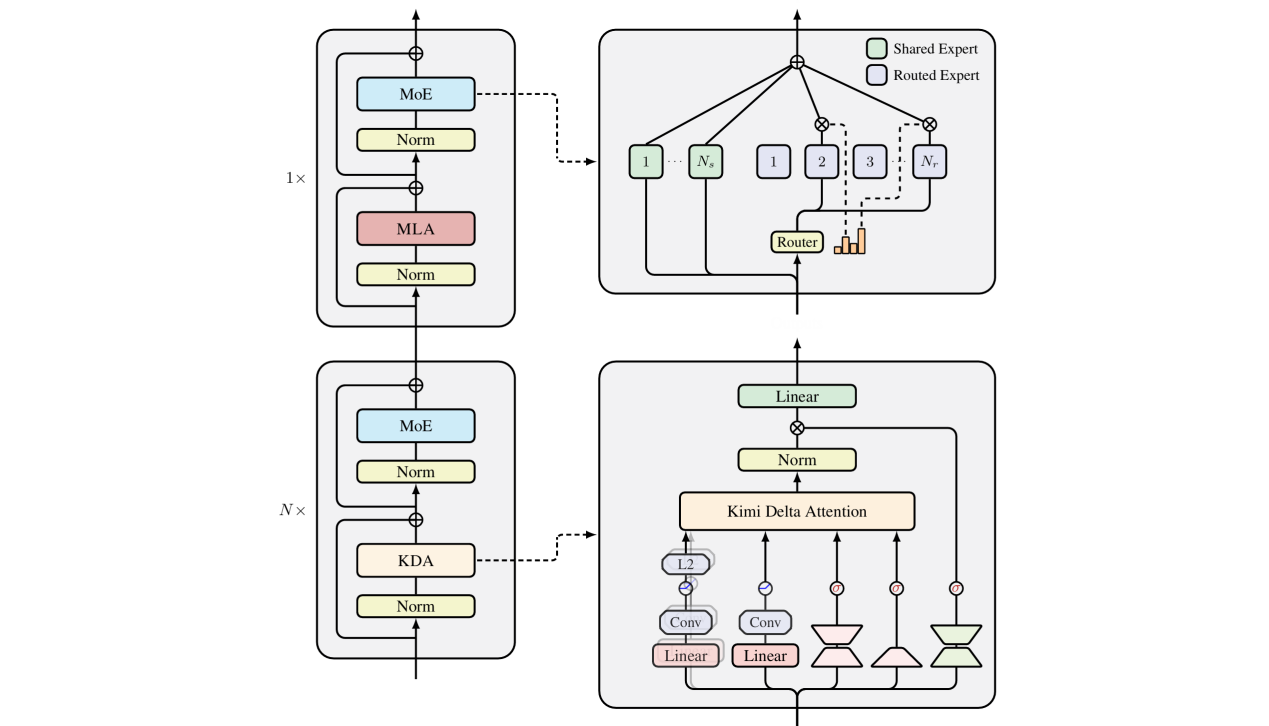
\includegraphics{images/image-0045.png}
\caption{Kimi Delta Attention 混合架构示意图}
\end{figure}

\hypertarget{ux56dbkdaux4e0ernn}{%
\subsection{四、KDA与RNN}\label{ux56dbkdaux4e0ernn}}

从原理上看，KDA本质上是一种RNN。那么，为什么KDA比传统RNN架构（如LSTM）效果更好呢？

\begin{enumerate}
\def\labelenumi{\arabic{enumi}.}
\item
  隐状态容量：LSTM的隐状态为d维向量，KDA的隐状态为d*d维矩阵。
\item
  能否利用GPU大规模并行训练
\end{enumerate}

在模型训练阶段，处理一个包含成千上万 token 的长文本时：

\begin{itemize}
\tightlist
\item
  LSTM 是被串行锁死的。LSTM 的状态更新公式是 \(h_t=\tanh(Wx_t+Uh_{t-1})\)，注意那个非线性激活函数 \(\tanh\)。它导致你必须等第 \(t-1\) 步的计算彻底完成，拿出确切的 \(h_{t-1}\) 后，才能开始算第 \(t\) 步。在拥有成千上万个流处理器的 GPU 面前，LSTM 只能排队一个一个算，GPU 算力被大量闲置。
\item
  KDA 是线性可并行的（Linear Recurrence）。忽略具体系数，KDA 的骨架公式可以写成：
\end{itemize}

\[
S_t=A_tS_{t-1}+V_t
\]

这个公式关于隐藏状态 \(S\) 是完全线性的（没有 \(\tanh\) 或 Sigmoid 阻挡）。根据矩阵乘法的结合律（Associativity），我们可以把时间序列展开：

\[
S_3=A_3(A_2S_1+V_2)+V_3=(A_3A_2)S_1+A_3V_2+V_3
\]

具体而言，对于推理的两个阶段：

A. 反馈集成阶段（Prefill 模式）：支持 token 间并行

当环境返回一段新的文本（例如搜索结果或环境状态变化）时，KDA 不需要像 RNN 那样一个 token 一个 token 地串行更新状态。

\begin{itemize}
\tightlist
\item
  Chunkwise-Parallel Algorithm：KDA 利用了线性注意力的结合律（Associativity）。通过数学变换，它可以将递推公式转化为块并行（Chunkwise）形式。
\item
  实现方式：如果环境反馈了 \(L\) 个 token，KDA 可以将这 \(L\) 个 token 作为一个``块''，在 GPU 上利用 Tensor Core 进行高并发的矩阵运算。一次运行即可处理完这 \(L\) 个 token，并直接得到最终的状态 \(S_{t+L}\)。
\item
  对比：传统模型处理新反馈时，KV Cache 的计算复杂度随总长度二次增长；而 KDA 处理新反馈的复杂度与总长度成线性关系。
\end{itemize}

B. 文本生成阶段（Decoding 模式）：单次运行生成，不可 token 间并行

当模型基于反馈开始生成新的回复（Action）时：

\begin{itemize}
\tightlist
\item
  单次运行：每生成一个新 token，确实只需要进行一次 \(O(1)\) 复杂度的前向传播。因为它只需读取上一步的状态 \(S_{t-1}\) 并计算 \(S_t\)，不需要重新扫描之前的全部上下文。
\item
  并行性限制：由于是自回归（Autoregressive）生成，token \(N+1\) 必须依赖 token \(N\) 生成后的状态。因此，在生成阶段无法实现 token 间并行（除非配合投机采样等技术）。
\end{itemize}

当然，这里如果环境反馈的序列较长，为了适配GPU，我们往往会进行分块处理，以一定量token作为一个块。

但总之，KDA可以运用FlashAttention这样的算子进行加速。

\begin{enumerate}
\def\labelenumi{\arabic{enumi}.}
\setcounter{enumi}{2}
\tightlist
\item
  数学本质：LSTM的更新是``启发式（Heuristic）''的：LSTM内部的遗忘门、输入门，是前人凭借直觉和实验凑出来的公式。网络只是隐式地学到一个``门限值''来决定保留什么、丢弃什么，它的本质是一个特征过滤器。
\end{enumerate}

KDA的更新是``第一性原理（First Principles）''的：如我们上一轮的推导，KDA的更新公式严格等价于在线梯度下降，即在线训练一个内部的线性回归模型。

面对新数据，KDA会算出预测误差，然后精准地沿着梯度的反方向修改记忆矩阵 \(S_t\)。这种严格的数学底座，使得KDA在处理复杂的逻辑推理和上下文学习（In-context Learning）时，拥有了碾压传统RNN的上限。

\hypertarget{ux4e94kdaux4e0eux5143ux5b66ux4e60}{%
\subsection{五、KDA与元学习}\label{ux4e94kdaux4e0eux5143ux5b66ux4e60}}

我们可以认为KDA是一种元学习（Meta-Learning）架构。在标准Transformer中，这种元学习是隐式的。而KDA将其变成了显式。

\begin{enumerate}
\def\labelenumi{\arabic{enumi}.}
\tightlist
\item
  外层循环：学习``如何在上下文中学习''
\end{enumerate}

在预训练阶段，我们在成千上万个 GPU 上使用标准的优化器（比如 AdamW），通过海量语料去更新 KDA 的物理参数，即用来生成 \(q,k,v\) 的投影权重 \(W_Q,W_K,W_V\)，以及遗忘门控 \(\alpha,\beta\)。

这些物理参数就是``元参数（Meta-parameters）''。AdamW 并没有教模型具体的知识，它是在教模型：

\begin{itemize}
\tightlist
\item
  遇到什么样的数据应该分配多大的学习率 \(\beta\)。
\item
  遇到什么特征应该开启遗忘门 \(\alpha\)。
\item
  如何从文本中提取最适合计算残差的 \(k\) 和 \(v\)。
\end{itemize}

\begin{enumerate}
\def\labelenumi{\arabic{enumi}.}
\setcounter{enumi}{1}
\tightlist
\item
  内层循环：在线梯度下降
\end{enumerate}

当模型部署后，你给它输入了一段长长的 Prompt。此时，物理参数（元参数）被冻结了，AdamW 优化器也下线了。

但是，KDA 内部的记忆矩阵 \(S_t\) 被激活了。随着你输入的数据一步步流入，KDA 严格按照外层循环教它的那套 Delta Rule，即在线梯度下降公式：

\[
S_t=S_{t-1}+\beta_tk_t\left(v_t-k_t^\top S_{t-1}\right)
\]

在 \(t\) 时刻的token输入KDA层时，隐状态根据 \(k_t\) 和 \(v_t\) 进行梯度下降更新，从 \(S_{t-1}\) 变为 \(S_t\)，带上了 \(t\) 时刻新的信息，但同时也已经在前 \(t-1\) 次梯度下降中保留了前 \(t-1\) 个token的信息（以先验形式存储在 \(S_{t-1}\) 中）。\(q_t\) 通过富含上下文 \(t\) 个token信息的 \(S_t\)，就实现了通过上下文学习来完成新的任务。

\begin{enumerate}
\def\labelenumi{\arabic{enumi}.}
\setcounter{enumi}{2}
\tightlist
\item
  其他参数（如embedding层、输入投影）：学习先验知识
\end{enumerate}

模型内部的embedding层、输入投影（MLP层）在预训练中记住了``秦始皇是哪一年称帝的''等人类世界的各种先验知识。这些先验知识被压入模型的这些参数，构成了模型极其庞大的高维特征子空间，确保模型输入被映射到符合其实际意义的向量，输入注意力层，如输入``苹果''时，MLP 瞬间把它映射到一个包含了``水果、红色、科技公司、牛顿''等无穷语义的特征坐标系中。

此外，对于输入的token，模型会根据先验参数判断是否需要启动上下文学习机制。如果问一个单纯的常识问题（比如``法国的首都是？''），模型根本不需要启动复杂的在下文梯度下降，它的MLP（先验知识）直接就能把``巴黎''的特征输出出来，此时 \(W_0\ne 0\) 而后续注意力层的 \(\Delta W\to 0\)。而对于模型在训练时没有见过的分布，会让 \(W_0\to 0\)（几乎没有先验，避免干扰上下文学习），而交给后续的 \(\Delta W\) 自主分析。

\hypertarget{ux53c2ux8003ux6587ux732e-137}{%
\subsection{参考文献}\label{ux53c2ux8003ux6587ux732e-137}}

\begin{itemize}
\tightlist
\item
  Moonshot AI. (2025). \href{https://arxiv.org/abs/2510.26692}{Kimi Linear: An Expressive, Efficient Attention Architecture}. arXiv:2510.26692.
\end{itemize}

\clearpage

\hypertarget{ux57faux4e8eux4e0aux4e0bux6587ux7684ux5143ux5f3aux5316ux5b66ux4e60ux8bbaux6587}{%
\section{基于上下文的元强化学习（论文）}\label{ux57faux4e8eux4e0aux4e0bux6587ux7684ux5143ux5f3aux5316ux5b66ux4e60ux8bbaux6587}}

\begin{quote}
本文是论文阅读笔记，内容代表对应论文方法或作者理解，不应直接视为领域共识或工程最佳实践。
\end{quote}

\hypertarget{ux4e00ux5143ux5f3aux5316ux5b66ux4e60ux7684ux57faux672cux601dux60f3}{%
\subsection{一、元强化学习的基本思想}\label{ux4e00ux5143ux5f3aux5316ux5b66ux4e60ux7684ux57faux672cux601dux60f3}}

元强化学习（Meta-RL）的目标不是让智能体掌握某一个具体任务，而是让智能体掌握一种学习策略。通过在大量的不同任务分布p(T)上进行元训练，从而在面对未见过的全新任务时，能够利用极少量的交互数据（Few-shot）实现快速适应。

一个强化学习任务 \(\mathcal{T}_i\) 可以被定义为一个马尔可夫决策过程（MDP）：

\[
\mathcal{T}_i = \{\mathcal{S}, \mathcal{A}, p_i(s_{t+1}\mid s_t,a_t), r_i(s_t,a_t), \gamma, H\}
\]

其中：

\begin{itemize}
\tightlist
\item
  \(\mathcal{S}, \mathcal{A}\)：状态空间和动作空间（通常假设跨任务共享）。
\item
  \(p_i(s_{t+1}\mid s_t,a_t)\)：状态转移概率（不同任务可能不同，如机器人的摩擦系数变化）。
\item
  \(r_i(s_t,a_t)\)：奖励函数（不同任务可能不同，如目标方向变化）。
\item
  \(H\)：时间视界（Horizon）。
\end{itemize}

Meta-RL 假设存在一个任务分布 \(p(\mathcal{T})\)。我们的目标是找到一组元参数（Meta-parameters）\(\theta\)，使得智能体在从分布中采样出的新任务 \(\mathcal{T}\sim p(\mathcal{T})\) 上，经过 \(K\) 步更新（或 \(K\) 条轨迹的适应）后，累积奖励最大化。

数学上，最大化目标函数 \(J(\theta)\)：

\[
\max_{\theta} J(\theta) =
\sum_{\mathcal{T}_i\sim p(\mathcal{T})}
\mathbb{E}_{\tau\sim p_{\mathcal{T}_i}(\tau\mid f_{\theta})}
[R(\tau)]
\]

其中，\(f_{\theta}\) 是由 \(\theta\) 参数化的适应过程（Adaptation Procedure），\(\tau\) 是轨迹。

\hypertarget{ux4e8cux57faux4e8eux4e0aux4e0bux6587ux7684ux5143ux5f3aux5316ux5b66ux4e60ux6982ux8ff0}{%
\subsection{二、基于上下文的元强化学习概述}\label{ux4e8cux57faux4e8eux4e0aux4e0bux6587ux7684ux5143ux5f3aux5316ux5b66ux4e60ux6982ux8ff0}}

我们已经知道，Transformer本质上等价于在上下文上作梯度下降，它本身就是一个持续学习的优化器。因此，对基于Transformer的大模型进行强化学习训练，本质上就是一个元学习过程，只不过没有显式地求二阶Hessian矩阵。因此，可以基于上下文设计元强化学习算法。

另一种思路是适应新任务本质上是一个部分可观察马尔可夫决策过程（POMDP）中的推断问题。在这种范式下，策略网络的权重在面对新任务时是固定不变的（不需要梯度下降）。相反，智能体会将过去的交互经验（状态、动作、奖励的序列）编码为一个隐变量（Latent Context/Representation）。策略网络只要通过将此上下文作为额外的输入条件，就可以隐式地改变其在不同任务中的行为。

下面介绍基于上下文的元强化学习算法。这些算法虽然在现在鲜有被直接提及，但却隐式地体现在现在的大模型中。

\hypertarget{ux4e09rl2}{%
\subsection{\texorpdfstring{三、RL\(^2\)}{三、RL\^{}2}}\label{ux4e09rl2}}

\hypertarget{ux4e00ux57faux672cux539fux7406ux548cux67b6ux6784}{%
\subsubsection{（一）基本原理和架构}\label{ux4e00ux57faux672cux539fux7406ux548cux67b6ux6784}}

在传统的单任务 RL 中，智能体面对环境只接收当前状态 \(s_t\)。但在 RL\(^2\) 中，为了让网络知道自己刚刚的``试错''是否有效，它必须拥有工作记忆（Working Memory）。

在传统的单任务 RL 中，智能体只接收当前状态 \(s_t\)。但在 RL\(^2\) 中，为了让网络知道自己刚才``试错''的结果，网络在时间步 \(t\) 的输入不仅包含当前状态 \(s_t\)，还包含上一步的动作 \(a_{t-1}\)、上一步的奖励 \(r_{t-1}\) 以及当前是否为回合结束的标志 \(d_{t-1}\)。

设输入向量为 \(x_t=(s_t,a_{t-1},r_{t-1},d_{t-1})\)。RL\(^2\) 使用循环神经网络（如 LSTM 或 GRU）来处理这个序列：

\[
h_t = f_{\theta}(x_t,h_{t-1})
\]

策略直接由隐藏状态生成：

\[
\pi_{\theta}(a_t\mid h_t)
\]

在这里，发生了两个时间尺度的学习：

\begin{itemize}
\tightlist
\item
  \textbf{慢速 RL（外环 Meta-training）}：也是权重更新的过程。在成千上万个不同的任务上，使用策略梯度算法（如 PPO 或 TRPO）来更新 RNN 的网络权重 \(\theta\)。
\item
  \textbf{快速 RL（内环 Adaptation）}：也是隐藏状态演化的过程。在面对一个全新任务时，权重 \(\theta\) 保持固定不动。智能体通过与环境交互，不断将 \((s,a,r)\) 喂给 RNN，RNN 的隐藏状态 \(h_t\) 随之更新。这个持续演化的 \(h_t\) 实际上充当了该任务的工作记忆（Working Memory）或信念状态（Belief State），从而瞬间改变了策略输出。
\end{itemize}

\hypertarget{ux4e8cux5de5ux4f5cux6d41-2}{%
\subsubsection{（二）工作流}\label{ux4e8cux5de5ux4f5cux6d41-2}}

\begin{enumerate}
\def\labelenumi{\arabic{enumi}.}
\tightlist
\item
  采样任务：从任务分布 \(p(\mathcal{T})\) 中采样一批任务。
\item
  构建序列（Trials）：对于每一个任务，执行 \(N\) 个回合（Episodes），这 \(N\) 个回合拼接成一个超长的序列（称为一个 Trial）。

  \begin{itemize}
  \tightlist
  \item
    关键点：在同一个 Trial（即同一个任务）内的不同 Episode 之间，RNN 的隐藏状态 \(h\) 不重置，而是保留下来跨回合传递。
  \item
    只有在切换到另一个全新任务时，隐藏状态 \(h\) 才会被清零。
  \end{itemize}
\item
  计算回报：累计整个 Trial 中所有回合的总奖励。
\item
  权重更新：将这些长序列数据输入到 TRPO 或 PPO 算法中，最大化期望总奖励，计算梯度并更新 RNN 权重 \(\theta\)。
\end{enumerate}

\hypertarget{ux4e09ux5b9eux73b0ux63a2ux7d22ux4e0eux5229ux7528ux5e73ux8861ux7684ux673aux5236}{%
\subsubsection{（三）实现探索与利用平衡的机制}\label{ux4e09ux5b9eux73b0ux63a2ux7d22ux4e0eux5229ux7528ux5e73ux8861ux7684ux673aux5236}}

RL\(^2\) 实现探索与利用的机制是完全隐式的（Implicit），由 RNN 在元训练中自己``悟''出来。

\begin{itemize}
\tightlist
\item
  \textbf{隐式的结构化探索}：假设任务是在迷宫中寻找一个随机放置的目标。在 Trial 的第 1 个回合（探索期），由于 \(h_0\) 是空的，RNN 会输出一些``扫描''策略（比如系统性地遍历每个房间）。在这个过程中，它虽然没得到奖励，但它记录了哪些地方去过（通过 \(x_t\) 中的 \(a\) 和 \(s\) 更新到 \(h\) 中）。
\item
  \textbf{向利用的自动切换}：一旦在某个时间步碰到了目标，收到了正奖励 \(r_{t-1}>0\)，这个信号就会输入给 RNN 并大幅改变隐藏状态 \(h_t\)。在随后的第 2 到第 \(N\) 个回合中（利用期），包含了``目标位置记忆''的隐藏状态 \(h_t\) 会直接驱使策略以最短路径走向目标。
\item
  \textbf{元目标驱动}：因为外环 PPO 优化的目标是最大化整个 Trial（\(N\) 个回合）的总收益，这就迫使 RNN 必须在最初的几个回合中采取高效率的试错行动（探索），以便在后续的回合中能够一直拿到最高分（利用）。
\end{itemize}

\hypertarget{ux56dbkimi-delta-attentionux4e2dux9690ux5f0fux7684rl2}{%
\subsubsection{\texorpdfstring{（四）Kimi Delta Attention中隐式的RL\(^2\)}{（四）Kimi Delta Attention中隐式的RL\^{}2}}\label{ux56dbkimi-delta-attentionux4e2dux9690ux5f0fux7684rl2}}

Kimi Delta Attention维护的线性注意力层本质上就可以视为RNN，从而本质上来说，在RL训练时这就是一个RL\(^2\) 算法：隐状态在每一个token生成（每一个epoch）后不会被清空，直到任务完成才会被重置。它的效果优于传统的RL\(^2\)，这是因为：

在原始的 RL\(^2\) 论文中，作者使用的是 LSTM 或 GRU，但这带来了严重的瓶颈，而 KDA 能有效解决这些痛点：

\begin{itemize}
\tightlist
\item
  \textbf{Meta-training 阶段的并行化加速}：LSTM 在训练（外环）时必须使用 BPTT（沿时间反向传播），只能一步步串行计算。而 KDA 作为线性注意力，在训练时可以通过\textbf{关联形式（Associative Form）}或\textbf{Chunkwise 并行计算机制}，像 Transformer 一样并行处理整个长序列。这极大地缩短了 Meta-RL 中极其漫长的外环训练时间。
\item
  \textbf{细粒度长程记忆控制}：传统 LSTM 的门控是粗粒度的。KDA 引入了通道级（Channel-wise）门控，让每个隐状态的维度独立决定记忆衰减。这意味着网络可以学到：用某些通道去锁死``目标全局坐标''这种绝对不能遗忘的信息（门控值接近 1），用另一些通道去记录``刚才走过哪个路口''的短期信息（快速衰减），从而在漫长的 Trial 中保持记忆的精度。
\end{itemize}

本质上来说，现在的Agentic RL就可以视为RL\(^2\) 的一种演进：

\begin{itemize}
\tightlist
\item
  \textbf{隐式到显式}：RL\(^2\) 将过去回合的试错经验压缩在 RNN 的隐状态 \(h_t\) 或 KDA 的 \(S_t\) 矩阵中；而 Agentic RLVR 将带有环境反馈的试错经验（``我刚才试了这段代码，服务器报了 404，所以我现在换个 API 试试''）以显式自然语言 Token 的形式写在了上下文窗口（KV Cache）中。
\item
  \textbf{学会探索（Learning to Explore）}：在 Agentic RLVR 的 Meta-training（外环权重更新）过程中，大模型逐渐学会了一种通用的、面对真实世界未知环境的探索策略。比如，当接到一个陌生任务时，它学会的第一步不再是盲目写代码，而是输出 \texttt{\textless{}action\textgreater{}\ ls\ -la\ \textless{}/action\textgreater{}} 或 \texttt{\textless{}action\textgreater{}\ cat\ README.md\ \textless{}/action\textgreater{}} 来探测环境状态。
\item
  \textbf{跨回合（Cross-episode）泛化}：只要环境的反馈被记录在上下文中，模型在测试阶段（权重 \(\theta\) 冻结）就能通过阅读前几步的真实报错 \((o_t)\)，利用注意力机制改变随后的动作 \((a_{t+1})\)，实现与真实世界的动态博弈和自适应修正。
\end{itemize}

\hypertarget{ux56dbpearl}{%
\subsection{四、PEARL}\label{ux56dbpearl}}

\hypertarget{ux4e00ux6838ux5fc3ux67b6ux6784}{%
\subsubsection{（一）核心架构}\label{ux4e00ux6838ux5fc3ux67b6ux6784}}

\begin{enumerate}
\def\labelenumi{\arabic{enumi}.}
\tightlist
\item
  \textbf{概率上下文编码器（Probabilistic Context Encoder）}
\end{enumerate}

在面对一个任务时，智能体会收集到一系列交互经验（Transitions），这些经验被称为上下文（Context），记为 \(c_{1:N}=\{(s_1,a_1,r_1,s'_1),\ldots,(s_N,a_N,r_N,s'_N)\}\)。

为了不像 RNN 那样严格依赖序列顺序，PEARL 设计了一个置换不变（Permutation-invariant）的编码器 \(q_{\phi}(\mathbf{z}\mid\mathbf{c})\)。它假设上下文中的每一次状态转移都是独立提供任务信息的。因此，编码器将每个转移元组 \((s,a,r,s')\) 通过多层感知机（MLP）映射为一个独立的高斯分布，然后将所有分布连乘起来，得到最终的后验隐变量分布：

\[
q_{\phi}(\mathbf{z}\mid\mathbf{c}_{1:N})
\propto
\prod_{n=1}^{N}
\mathcal{N}\left(f_{\phi}^{\mu}(c_n), f_{\phi}^{\Sigma}(c_n)\right)
\]

其中，\(\mathbf{z}\) 就是代表当前任务特征的连续隐变量，\(f_{\phi}^{\mu}\) 和 \(f_{\phi}^{\Sigma}\) 分别是输出均值和方差的网络。

\begin{enumerate}
\def\labelenumi{\arabic{enumi}.}
\setcounter{enumi}{1}
\tightlist
\item
  \textbf{条件 Actor-Critic 网络（Context-conditioned Actor-Critic）}
\end{enumerate}

PEARL 的底层强化学习算法通常基于 SAC（Soft Actor-Critic）。在推断出隐变量 \(z\) 后，\(z\) 会作为额外的输入，与当前状态 \(s\) 一起喂给策略网络和价值网络：

\begin{itemize}
\tightlist
\item
  Actor 网络（策略）：\(\pi_{\theta}(a\mid s,z)\)
\item
  Critic 网络（Q 值）：\(Q_{\theta}(s,a,z)\)
\end{itemize}

这意味着，网络权重 \(\theta\) 在不同任务之间是完全共享且固定的，策略的改变仅仅依赖于前向传播时输入的 \(z\) 的变化。

\hypertarget{ux4e8cux635fux5931ux51fdux6570}{%
\subsubsection{（二）损失函数}\label{ux4e8cux635fux5931ux51fdux6570}}

\begin{enumerate}
\def\labelenumi{\arabic{enumi}.}
\tightlist
\item
  \textbf{编码器的 KL 散度正则化}
\end{enumerate}

为了防止编码器对某一个具体的上下文序列过拟合，PEARL 强制后验分布 \(q_{\phi}(z\mid c)\) 逼近一个先验分布 \(p(z)\)（通常设为标准正态分布 \(\mathcal{N}(0,I)\)）。这通过最小化 KL 散度来实现：

\[
\mathcal{L}_{KL}(\phi)=\beta D_{KL}(q_{\phi}(z\mid c)\|p(z))
\]

其中 \(\beta\) 是调节信息瓶颈强度的超参数。

\begin{enumerate}
\def\labelenumi{\arabic{enumi}.}
\setcounter{enumi}{1}
\tightlist
\item
  \textbf{Critic 与 Actor 的损失函数}
\end{enumerate}

Critic 的更新目标是最小化引入了 \(z\) 的贝尔曼残差（Bellman Error）：

\[
\mathcal{L}_{critic}(\theta,\phi)=
\mathbb{E}_{(s,a,r,s')\sim\mathcal{B},z\sim q_{\phi}}
\left[
\left(
Q_{\theta}(s,a,z)-
(r+\gamma V_{\bar{\theta}}(s',z))
\right)^2
\right]
\]

这里的目标价值函数 \(V_{\bar{\theta}}\) 包含了 SAC 特有的熵最大化项（\(\alpha\) 为温度系数）：

\[
V_{\bar{\theta}}(s',z)=
\mathbb{E}_{a'\sim\pi_{\theta}}
\left[
Q_{\bar{\theta}}(s',a',z)-
\alpha\log\pi_{\theta}(a'\mid s',z)
\right]
\]

Actor 的更新目标则是最大化期望 Q 值并同时最大化策略熵：

\[
\mathcal{L}_{actor}(\theta)=
\mathbb{E}_{s\sim\mathcal{B},z\sim q_{\phi},a\sim\pi_{\theta}}
\left[
\alpha\log\pi_{\theta}(a\mid s,z)-
Q_{\theta}(s,a,z)
\right]
\]

在元训练期间，来自 Critic 损失的梯度会反向传播流经 \(z\)，从而更新编码器参数 \(\phi\)，迫使编码器提取那些``对预测奖励和价值最有用''的上下文信息。

\hypertarget{ux4e09ux8badux7ec3ux5de5ux4f5cux6d41-1}{%
\subsubsection{（三）训练工作流}\label{ux4e09ux8badux7ec3ux5de5ux4f5cux6d41-1}}

\begin{enumerate}
\def\labelenumi{\arabic{enumi}.}
\tightlist
\item
  \textbf{初始化}：初始化网络参数 \(\phi,\theta\)，为每个训练任务 \(\mathcal{T}_i\) 初始化空的重放缓冲区 \(\mathcal{B}_i\)。
\item
  \textbf{数据收集循环}：

  \begin{itemize}
  \tightlist
  \item
    从任务分布 \(p(\mathcal{T})\) 中采样一个任务 \(\mathcal{T}_i\)。
  \item
    初始化当前任务的上下文 \(c^i=\varnothing\)。
  \item
    \textbf{后验采样探索}：在每个 Episode 开始前，使用编码器计算分布并采样隐变量 \(\mathbf{z}\sim q_{\phi}(\mathbf{z}\mid\mathbf{c}^i)\)。在这个 Episode 内，\(\mathbf{z}\) 保持固定不变。
  \item
    智能体使用策略 \(\pi_{\theta}(a\mid s,\mathbf{z})\) 与环境交互，收集数据 \((s,a,r,s')\) 并将其存入缓冲区 \(\mathcal{B}_i\) 中。
  \item
    更新上下文 \(\mathbf{c}^i\leftarrow\mathbf{c}^i\cup\{(s,a,r,s')\}\)。
  \end{itemize}
\item
  \textbf{网络优化循环}：

  \begin{itemize}
  \tightlist
  \item
    随机采样一个批次（Batch）的任务。
  \item
    对于每个任务，从其对应的 \(\mathcal{B}_i\) 中随机抽取两组不相交的批次数据：

    \begin{itemize}
    \tightlist
    \item
      上下文批次 \(c^{batch}\)：送入编码器，推断出 \(z\) 的分布。
    \item
      RL 训练批次 \(b^{batch}\)：用于计算 SAC 损失。
    \end{itemize}
  \item
    从分布中采样 \(z\)，计算 \(\mathcal{L}_{critic}\)、\(\mathcal{L}_{actor}\) 和 \(\mathcal{L}_{KL}\)。
  \item
    使用梯度下降法联合更新参数 \(\phi\) 和 \(\theta\)。
  \end{itemize}
\end{enumerate}

\hypertarget{ux56dbagentic-rlux672cux8d28ux4e0aux662fpearlux7b49context-based-meta-rlux7b97ux6cd5ux7684ux6f14ux8fdb}{%
\subsubsection{（四）Agentic RL本质上是PEARL等Context-based Meta-RL算法的演进}\label{ux56dbagentic-rlux672cux8d28ux4e0aux662fpearlux7b49context-based-meta-rlux7b97ux6cd5ux7684ux6f14ux8fdb}}

无论是 PEARL 还是 Agentic RL，它们解决问题的核心数学公式是完全等价的：在测试阶段冻结网络权重 \(\theta\)，依靠不断增长的历史交互 \(C\)，来推断当前任务并输出最优动作 \(a_0\)。

\begin{itemize}
\tightlist
\item
  \textbf{Context-based Meta-RL（如 PEARL）}：策略网络的形式为 \(\pi_{\theta}(a_t\mid s_t,C_{1:t-1})\)。其中，上下文 \(C=\{(s_1,a_1,r_1,s_2),\ldots\}\) 是一堆交互经验。PEARL 使用一个编码器将 \(C\) 压缩成一个连续的隐变量 \(z\)，然后 Actor 根据 \(z\) 输出动作。
\item
  \textbf{Agentic RL（基于 LLM）}：策略网络（LLM）的形式为 \(\pi_{\theta}(a_t\mid\mathrm{Prompt}_t)\)。这里的 Prompt，就是上下文。它忠实地记录了历史轨迹：用户指令 \((s_0)\)、模型调用的工具代码 \((a_{1:t-1})\)、环境返回的终端报错或网页内容 \((s_{1:t})\)，以及客观奖励反馈 \((r_{1:t-1})\)。LLM 通过自注意力机制（Self-Attention）处理这段 Prompt，直接输出下一步的动作。
\end{itemize}

二者在数学上是同构的，只是状态载体发生了变化：从隐式、不可读的高维连续向量（\(z\) 或 \(h_t\)），变成了显式、人类可读的离散 Token 序列（KV Cache 中的文本）。

具体来说：

\begin{enumerate}
\def\labelenumi{\arabic{enumi}.}
\tightlist
\item
  \textbf{上下文记忆（Context c）}：

  \begin{itemize}
  \tightlist
  \item
    PEARL：记忆是一个无序的经验回放集合 \(\mathbf{c}=\{(s_i,a_i,r_i,s_{i+1})\}_{i=0}^{N}\)。
  \item
    LLM Agent：记忆是\textbf{上下文窗口（Context Window）}中拼接的 Token 序列（包含了 System Prompt、之前的动作命令、环境返回的真实终端报错以及步骤得分）。
  \end{itemize}
\item
  \textbf{任务推断与隐变量（Encoder \(q_{\phi}\) \& Latent \(z\)）}：

  \begin{itemize}
  \tightlist
  \item
    PEARL：使用基于 MLP 的概率编码器，输出一个连续的高斯分布隐变量 \(z\sim\mathcal{N}(\mu,\sigma^2)\)。\(z\) 代表了网络对当前陌生任务的``信念''。
  \item
    LLM Agent：LLM 的多头自注意力机制（Self-Attention）充当了天然的编码器，而深层的 KV Cache 构成了高维隐状态。更进一步，在带有显式推理的 Agent 中，模型通过生成``反思文本（Reflection / Chain-of-Thought）''，将对环境的推断显式地输出为了人类可读的 \(z\)。
  \end{itemize}
\item
  \textbf{策略网络（Actor \(\pi_{\theta}\)）}：

  \begin{itemize}
  \tightlist
  \item
    PEARL：策略是 \(\pi_{\theta}(a\mid s,z)\)，通过连续动作空间的强化学习算法更新。
  \item
    LLM Agent：策略是自回归语言建模头 \(\pi_{\theta}(a\mid\mathrm{Prompt},\mathrm{Reflection})\)，它在词表分布上进行温度采样，生成具体的 Python 代码或 Bash 命令。
  \end{itemize}
\end{enumerate}

虽然本质相同，但 Agentic RL 代表了 Meta-RL 演进的终极形态，它解决了传统 Meta-RL 的几个致命痛点：

\begin{enumerate}
\def\labelenumi{\arabic{enumi}.}
\tightlist
\item
  \textbf{极度泛化（从``白板''到``世界模型先验''）}：传统的 Meta-RL 是从零开始（Tabula Rasa）在特定环境中元训练的，它只能泛化到非常相似的同分布任务。而 Agentic LLM 已经通过海量互联网数据获得了极强的先验知识（世界模型）。它不需要再从头通过试错去学习``什么是 404 Error''或``什么是 Python 语法''，它可以直接调用预训练概念，实现真正意义上的 Zero-shot 或 Few-shot 跨域泛化。
\item
  \textbf{无损的长程信用分配}：无论是 RL\(^2\) 的 RNN 还是 PEARL 的高斯分布，在压缩几千步的 Trial 上下文时都会发生严重的信息丢失。而 Agentic RL 依托现代大模型的 KV Cache（或是你之前关注的 KDA 线性注意力机制），能够以极高的保真度保留极其久远的关键试错细节。
\item
  \textbf{显式的思维链（Chain-of-Thought）干预}：Agentic RL 可以在观测 \(o\) 和动作 \(a\) 之间，插入显式的推理想法。这种内部语言空间使得``探索逻辑''变得可解释，并且可以被外部规则（如 RLVR）进行精准的组内优势（Advantage）排序。
\end{enumerate}

\hypertarget{ux4e94llm-agent-with-meta-rllamer}{%
\subsection{五、LLM Agent with Meta-RL（LAMER）}\label{ux4e94llm-agent-with-meta-rllamer}}

\begin{enumerate}
\def\labelenumi{\arabic{enumi}.}
\tightlist
\item
  \textbf{跨回合训练框架（Cross-episode Training Framework）}
\end{enumerate}

LAMER 吸收了 RL\(^2\) 的宏观精髓，将环境交互的视距提升到了 Trial（试验）级别。

\begin{itemize}
\tightlist
\item
  一个完整的 Trial 包含多个独立的 Episode（回合）。
\item
  \textbf{奖励重塑}：算法优化的目标不再是单个回合的收益，而是跨回合折扣回报（Cross-episode discounted return）。
\end{itemize}

\[
J(\theta)=
\mathbb{E}_{\mathcal{T}\sim p(\mathcal{T}),\tau\sim\pi_{\theta}}
\left[
\sum_{k=1}^{K}\gamma^{k-1}R_k
\right]
\]

其中 \(K\) 是 Trial 内的总回合数，\(R_k\) 是第 \(k\) 个回合的总奖励。

\begin{itemize}
\tightlist
\item
  \textbf{探索的涌现}：这种严苛的奖励设计迫使大模型学会``放长线钓大鱼''。在早期的 Episode 中，模型会主动放弃眼前的安全低分，采取一些大概率会导致当前回合失败（但能探明环境机制或排除错误代码）的探索性动作。
\end{itemize}

\begin{enumerate}
\def\labelenumi{\arabic{enumi}.}
\setcounter{enumi}{1}
\tightlist
\item
  \textbf{结合自我反思的上下文策略适应（In-context Policy Adaptation via Self-Reflection）}
\end{enumerate}

这就是 PEARL 中生成推断隐变量 \(z\) 的最完美文本化体现。

LAMER 在测试（部署）阶段不进行任何网络参数的梯度更新。相反，在每一个 Episode 结束后（比如代码跑崩了），LAMER 会强制 LLM Agent 根据刚才积累的交互日志，生成一段纯文本的自我反思（Reflection）。

\begin{itemize}
\tightlist
\item
  这段反思文本会深入分析错误原因（例如：``我尝试向数组里 Append 字典，但引发了类型错误，因为接口需要 JSON 字符串''），并提出下一个回合的改进策略。
\item
  这个生成的 Reflection，会被作为强有力的先验上下文，直接 Prefix（前置拼接）到下一个 Episode \(k+1\) 的 Prompt 中。
\item
  依靠这种纯文本的演绎，Agent 的策略在下一个回合中发生了一次无需算力开销的 RL\(^2\) 飞跃。
\end{itemize}

\hypertarget{ux53c2ux8003ux6587ux732e-138}{%
\subsection{参考文献}\label{ux53c2ux8003ux6587ux732e-138}}

\begin{itemize}
\tightlist
\item
  Duan, Y., Schulman, J., Chen, X., Bartlett, P. L., Sutskever, I., \& Abbeel, P. (2016). \href{https://arxiv.org/abs/1611.02779}{RL\(^2\): Fast Reinforcement Learning via Slow Reinforcement Learning}. arXiv:1611.02779.
\item
  Rakelly, K., Zhou, A., Finn, C., Levine, S., \& Quillen, D. (2019). \href{https://arxiv.org/abs/1903.08254}{Efficient Off-Policy Meta-Reinforcement Learning via Probabilistic Context Variables}. ICML 2019.
\item
  Jiang, Y., Jiang, L., Teney, D., Moor, M., \& Brbic, M. (2025). \href{https://arxiv.org/abs/2512.16848}{Meta-RL Induces Exploration in Language Agents}. ICLR 2026.
\end{itemize}

\clearpage

\hypertarget{ux57faux4e8eux4e0aux4e0bux6587ux548cux957fux671fux8bb0ux5fc6ux7684ux6301ux7eedux5b66ux4e60ux8bbaux6587}{%
\section{基于上下文和长期记忆的持续学习（论文）}\label{ux57faux4e8eux4e0aux4e0bux6587ux548cux957fux671fux8bb0ux5fc6ux7684ux6301ux7eedux5b66ux4e60ux8bbaux6587}}

\begin{quote}
本文是论文阅读笔记，内容代表对应论文方法或作者理解，不应直接视为领域共识或工程最佳实践。
\end{quote}

\hypertarget{ux4e00ux591aux5c3aux5ea6ux8ba4ux77e5ux4ee5ml-masterux4e3aux4f8b}{%
\subsection{一、多尺度认知：以ML-Master为例}\label{ux4e00ux591aux5c3aux5ea6ux8ba4ux77e5ux4ee5ml-masterux4e3aux4f8b}}

\hypertarget{ux4e00ux6838ux5fc3ux67b6ux6784-1}{%
\subsubsection{（一）核心架构}\label{ux4e00ux6838ux5fc3ux67b6ux6784-1}}

HCC 将上下文分为三个层级，以应对不同时间尺度的认知需求：

\begin{itemize}
\tightlist
\item
  \(L_1\) 缓存：演进经验（Evolving Experience）

  \begin{itemize}
  \tightlist
  \item
    \textbf{作用}：作为智能体的工作记忆，保存当前执行所需的高保真原始轨迹（如当前的研究计划、代码补丁、终端报错和指标日志），用于即时调试和决策。
  \item
    \textbf{数学表达}：在当前阶段 \(p\) 的时间步 \(t\)，其缓存状态为 \(\mathcal{L}_1(t)=\mathcal{E}_{t_0-1}\cup\mathcal{P}_{p-1}\cup\mathcal{E}_{t_{p-1}+1:t}\)。其中 \(\mathcal{E}_{t_{p-1}:t}\) 是当前计划的原始执行轨迹。
  \end{itemize}
\item
  \(L_2\) 缓存：提炼知识（Refined Knowledge）

  \begin{itemize}
  \tightlist
  \item
    \textbf{作用}：作为中期战略记忆，存储从已完成的探索阶段中提炼出的稳定认知（如关键判断、实验洞察、精简的进度总结）。这让智能体在数十小时的探索中保持战略一致性，而无需携带冗长的执行日志。
  \item
    \textbf{数学表达}：\(\mathcal{L}_2(t)=\{\kappa_{t_{r-1}+1:t_r-1}\}_{r=1}^{p-1}\)，其中 \(\kappa\) 是通过大模型对原始事件片段进行提炼后得到的紧凑知识摘要。
  \end{itemize}
\item
  \(L_3\) 缓存：先验智慧（Prior Wisdom）

  \begin{itemize}
  \tightlist
  \item
    \textbf{作用}：作为长期记忆，存储跨任务可复用的抽象策略（如鲁棒的模型模板、数据处理流水线）。它使得智能体在面对新任务时能够``热启动''。
  \item
    \textbf{数学表达}：存储为嵌入-值对的集合 \(\mathcal{L}_3\triangleq(h_n,w_n)_{n=1}^{N}\)，其中 \(h_n\) 是检索键，\(w_n\) 是提炼出的任务级智慧文本。
  \end{itemize}
\end{itemize}

\hypertarget{ux4e8cux5de5ux4f5cux6d41-3}{%
\subsubsection{（二）工作流}\label{ux4e8cux5de5ux4f5cux6d41-3}}

为了在这三个缓存层之间动态流转信息，系统设计了严格的生命周期管理操作：

\begin{enumerate}
\def\labelenumi{\arabic{enumi}.}
\tightlist
\item
  \textbf{初始化与上下文预取（Context Prefetching）}：

  \begin{itemize}
  \tightlist
  \item
    给定新任务描述 \(d_{\tau}\)，系统计算其向量嵌入 \(q=E(d_{\tau})\)。
  \item
    通过余弦相似度阈值从 \(L_3\) 缓存中检索出相关的先验智慧：\(\Omega_{\tau}=\{w_n\mid(h_n,w_n)\in\mathcal{L}_3,\cos(q,h_n)>\delta\}\)。
  \item
    将检索到的智慧作为初始上下文，确保智能体在一个高起点的认知下开始探索。
  \end{itemize}
\item
  \textbf{执行与上下文命中（Context Hit）}：

  \begin{itemize}
  \tightlist
  \item
    在生成每一步的上下文时，系统优先从 \(L_1\) 提取当前活跃阶段的原始经验。
  \item
    对于过去已经完成的阶段，则退回到 \(L_2\) 提取高度浓缩的提炼知识。这有效防止了上下文饱和。
  \end{itemize}
\item
  \textbf{整合与上下文晋升（Context Promotion）}：

  \begin{itemize}
  \tightlist
  \item
    \textbf{阶段级晋升（\(P_1\)）}：当一个探索阶段结束时，智能体会利用 LLM 的总结能力，将 \(L_1\) 中的原始并行探索轨迹压缩成一个精炼的知识单元 \(\kappa_p\)，写入 \(L_2\)，并从 \(L_1\) 中清理掉对应的原始数据。
  \item
    \textbf{任务级晋升（\(P_2\)）}：当整个机器学习任务完成后，系统会从全局视角提取可复用的策略 \(w_{\tau}\)，并将其固化到 \(L_3\) 缓存中，供未来的任务检索使用。
  \end{itemize}
\end{enumerate}

\hypertarget{ux4e8cux8f7bux91cfux7ea7ux5206ux5c42ux8bb0ux5fc6lightmem}{%
\subsection{二、轻量级分层记忆：LightMem}\label{ux4e8cux8f7bux91cfux7ea7ux5206ux5c42ux8bb0ux5fc6lightmem}}

LightMem模仿人类的记忆系统，把记忆系统拆成三个轻量模块：

Light1：感官记忆（Sensory Memory），快速过滤无用信息、把输入压缩到``值得记''的部分，并进行主题切分。

具体做法：使用一个轻量压缩模型，在切分时避免``按窗口切''的粗暴做法，而是用注意力信号的峰值找到候选topic边界（见后），再用相邻片段的语义相似度做二次确认，取二者交集作为最终切分点，降低attention sink、注意力稀释等噪声影响导致的``伪峰值''。

怎么用注意力信号找到topic边界：让一个小参数量的语言模型先快速``读''一遍文本，当话题突变，可观察到新Token对旧话题Token的注意力权重 \(A_{i,j}\) 急剧下降，模型为了满足Softmax的归一化特性，会将注意力强制转移到新话题的起始Token上，这些位置就会形成注意力的局部峰值，通过找出峰值即可确定话题突变位置。

Light2：短时记忆（Short-Term Memory, STM），按主题把对话组织成结构化单元，降低总结调用次数，同时减少主题混杂。

具体做法：在拿到topic segments后，以 \texttt{\{topic,\ turns\}} 的结构送入STM buffer。达到token阈值时，才触发一次LLM总结，对每个topic生成更结构化的summary，并写入LTM。相比``每一轮都总结一次''，这样调用次数降低：总结不再是 \(N\) 次，而是按buffer触发的更少次数；输入被topic约束，不容易``把A主题的细节总结进B主题里''。

Light3：长时记忆（Long-Term Memory, LTM）+睡眠更新（Sleep-time Update），把昂贵的记忆更新从在线推理中``拿出来''，在离线并行地做去重、合并、修复与巩固。

具体做法：为了避免在test time将短时记忆转为长时记忆导致延时，系统在测试时新记忆条目到来时，直接插入LTM，不做复杂更新。离线阶段（sleep time）触发更新，对每个条目构建一个update queue（只允许``新的更新旧的''，即时间戳约束 \(t_j\ge t_i\)），然后把这些更新操作并行执行。

\begin{figure}[htbp]
\centering
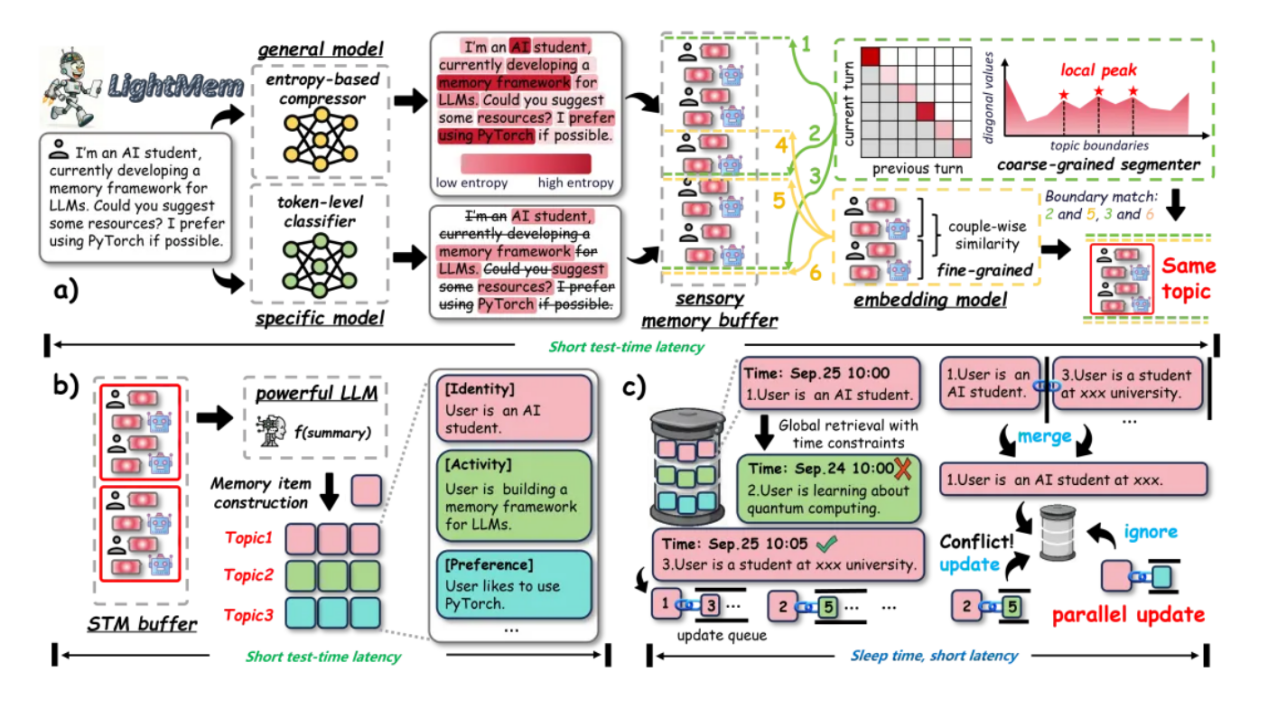
\includegraphics{images/image-0046.png}
\caption{LightMem 轻量级分层记忆系统示意图}
\end{figure}

\hypertarget{ux4e09ux751fux6210ux5668ux4e0eux8bb0ux5fc6ux7ba1ux7406ux667aux80fdux4f53ux534fux540cagentic-context-engineering}{%
\subsection{三、生成器与记忆管理智能体协同：Agentic Context Engineering}\label{ux4e09ux751fux6210ux5668ux4e0eux8bb0ux5fc6ux7ba1ux7406ux667aux80fdux4f53ux534fux540cagentic-context-engineering}}

\hypertarget{ux4e00ux6838ux5fc3ux67b6ux6784-2}{%
\subsubsection{（一）核心架构}\label{ux4e00ux6838ux5fc3ux67b6ux6784-2}}

\begin{enumerate}
\def\labelenumi{\arabic{enumi}.}
\item
  生成器（Generator）：接收新的查询并生成推理轨迹（包括有效策略和反复出现的陷阱） 。
\item
  反思器（Reflector）：批判这些生成的轨迹，从成功和错误中提取具体的经验教训，并可选择在多次迭代中进行提炼。同时，也给原有经验打上``有用''``有害''``中立''等标签。
\item
  策展人（Curator）：得到新的经验教训后，不重写上下文，而是将新的经验教训综合成紧凑的增量条目（delta entries）。这里的增量条目格式一般为``元数据（如ID，以及记录该条目被标记为``有用''或``有害''次数的计数器等）+内容（具体的策略、领域概念或常见错误等）''。
\item
  自动化脚本：得出增量条目后，将其确定性地合并到现有的上下文中。具体方式包括：（1）如果是一个带有新ID的新经验，直接追加到上下文列表的末尾；（2）如果是对某条旧规则的反馈，代码直接修改那条旧规则（比如把``有用''次数 +1）；（3）如果发现两条规则在向量空间相似度过高，就删除冗余。
\end{enumerate}

\hypertarget{ux4e8cux4e0aux4e0bux6587ux6e05ux7406ux673aux5236}{%
\subsubsection{（二）上下文清理机制}\label{ux4e8cux4e0aux4e0bux6587ux6e05ux7406ux673aux5236}}

作者认为，如果赋予大模型随意删除或重写整个上下文的权力，它往往会犯``简洁性偏见（Brevity Bias）''的毛病，为了追求简短和通用，大模型很容易把那些看起来有些繁琐但极其关键的``特定领域的启发式方法、工具使用指南或避坑细节''给丢弃掉。在ACE框架中，策展人（Curator）这个大模型角色本身并不负责直接发出``删除''指令，但整个系统确实存在一套机制来删除和清理原有经验，以防止上下文越积越多。

\begin{enumerate}
\def\labelenumi{\arabic{enumi}.}
\item
  语义去重与修剪：当策展人生成了新的经验条目后，底层的传统代码会计算所有经验条目的语义嵌入向量，若文本的语义上高度相似（即存在冗余），系统会自动执行去重并修剪掉多余的内容，用非LLM逻辑自动删除了重复的经验。
\item
  反思器的``有害''标记：在生成新经验之前，反思器（Reflector）会先对当前生成的轨迹进行复盘，并对上下文中被使用到的原有经验条目打上标签（helpful有用、harmful有害、neutral中立）。虽然策展人只负责输出需要添加的新洞察，但系统会根据反思器的标记来就地更新旧条目的计数器。这些指标可以帮助系统评估哪些经验是无效或起反作用的。
\item
  延迟提炼机制：修剪和提炼可以配置为主动进行（每次更新增量后都执行），也可以配置为延迟进行，即只有当上下文长度即将超出模型的上下文窗口限制时，才触发清理机制。
\end{enumerate}

\hypertarget{ux56dbux89c4ux5212ux4e0eux6267ux884cagentux7684ux8bb0ux5fc6ux5206ux79bbux5f0fux6301ux7eedux5b66ux4e60ux67b6ux6784}{%
\subsection{四、规划与执行Agent的记忆分离式持续学习架构}\label{ux56dbux89c4ux5212ux4e0eux6267ux884cagentux7684ux8bb0ux5fc6ux5206ux79bbux5f0fux6301ux7eedux5b66ux4e60ux67b6ux6784}}

\hypertarget{ux4e00ux57faux672cux601dux60f3-3}{%
\subsubsection{（一）基本思想}\label{ux4e00ux57faux672cux601dux60f3-3}}

在多智能体架构中，不同Agent负责规划、执行等，它们总结和需要使用的经验也会有所不同。因此，可将抽象的``规划逻辑''与具体的``执行技巧''分开提取、独立存储、分层检索。负责规划的Agent记忆（高层记忆）中往往是在给定总目标下，制定子目标、调度智能体等的方法和经验，负责执行的Agent记忆（底层记忆）中则是在具体子目标下执行的方法和经验。

\hypertarget{ux4e8cux8badux7ec3ux5de5ux4f5cux6d41}{%
\subsubsection{（二）训练工作流}\label{ux4e8cux8badux7ec3ux5de5ux4f5cux6d41}}

\begin{enumerate}
\def\labelenumi{\arabic{enumi}.}
\tightlist
\item
  \textbf{子目标推断（Subgoal Inference）}：
\end{enumerate}

给定一个任务 \(x\) 及其完整交互轨迹 \(\tau\)，利用大模型推断出该轨迹实际达成的一系列离散子目标序列 \(s_{1:N}\)。

\begin{enumerate}
\def\labelenumi{\arabic{enumi}.}
\setcounter{enumi}{1}
\tightlist
\item
  \textbf{子轨迹推断与分割（Subtrajectory Inference）}：
\end{enumerate}

根据推断出的子目标序列 \(s_{1:N}\)，将冗长、复杂的完整原始轨迹 \(\tau\) 在时间轴上切分为多个局部的子轨迹片段 \(\tau_{s_i}\)。这使得每一个子轨迹只专注于单一的子目标。

\begin{enumerate}
\def\labelenumi{\arabic{enumi}.}
\setcounter{enumi}{2}
\tightlist
\item
  \textbf{对比反思与洞察提取（Insight Extraction）}：
\end{enumerate}

这是最核心的``萃取''步骤。算法会同时对比同一任务下成功的轨迹 \(\tau^{+}\) 和失败的轨迹 \(\tau^{-}\)。

\begin{itemize}
\tightlist
\item
  \textbf{高层萃取}：对比成功的子目标序列和失败的序列，生成或更新全局的高层指导原则 \(I_{\mathrm{high}}\)（增加、修改、点赞或踩踏现有的 Rule）。
\item
  \textbf{底层萃取}：针对特定的子目标，对比成功和失败的子轨迹片段，提取出底层的避错原则 \(I_{\mathrm{low}}\)。
\end{itemize}

\begin{enumerate}
\def\labelenumi{\arabic{enumi}.}
\setcounter{enumi}{3}
\tightlist
\item
  \textbf{记忆单元组装与写入（Memory Unit Creation）}：
\end{enumerate}

将上述提取出的 \((x,s,I_{\mathrm{high}})\) 封装入 \(\mathcal{M}_{\mathrm{high}}\)；将 \((s_i,\tau_{s_i},I_{\mathrm{low}})\) 封装入 \(\mathcal{M}_{\mathrm{low}}\)。

\hypertarget{ux4e09ux6d4bux8bd5ux5de5ux4f5cux6d41}{%
\subsubsection{（三）测试工作流}\label{ux4e09ux6d4bux8bd5ux5de5ux4f5cux6d41}}

当面对一个全新的测试任务 \(x_{\mathrm{test}}\) 时，\(H^2R\) 采用``规划器（Planner）''与``执行器（Executor）''双重检索机制：

\begin{enumerate}
\def\labelenumi{\arabic{enumi}.}
\tightlist
\item
  \textbf{规划器检索（高层）}：
\end{enumerate}

规划器通过预训练的句向量编码器 \(\phi(\cdot)\) 计算当前任务与高层记忆库中历史任务的余弦相似度，检索出 Top-\(k\) 相关的规划记忆：

\[
\mathrm{sim}(x_{\mathrm{test}},x)=
\frac{\phi(x_{\mathrm{test}})\cdot\phi(x)}
{\|\phi(x_{\mathrm{test}})\|\|\phi(x)\|}
\]

结合检索到的经验，规划器将 \(x_{\mathrm{test}}\) 拆解为当前需要的子目标序列。

\begin{enumerate}
\def\labelenumi{\arabic{enumi}.}
\setcounter{enumi}{1}
\tightlist
\item
  \textbf{执行器检索（底层）}：
\end{enumerate}

对于规划器给出的当前子目标 \(s_{\mathrm{current}}\)，执行器以子目标为 Query，去底层记忆库 \(\mathcal{M}_{\mathrm{low}}\) 中进行相似度检索。根据检索到的底层交互技巧和子轨迹，执行器决定具体的原子动作（Atomic Actions），并判断该子目标是否已经完成或失效。

\hypertarget{ux4e94reactux7684ux6539ux8fdbremem}{%
\subsection{五、ReAct的改进：ReMem}\label{ux4e94reactux7684ux6539ux8fdbremem}}

在 ReMem 框架内，系统的整个决策循环被视为一个马尔可夫决策过程（Markov Decision Process）。

\begin{enumerate}
\def\labelenumi{\arabic{enumi}.}
\tightlist
\item
  \textbf{状态定义}：在时间步 \(t\) 且经过 \(n\) 次内部操作后，智能体的状态定义为 \(s_t^n=(x_t,M_t,o_t^{1:n-1})\)，即当前输入、当前记忆以及截至目前的推理轨迹 \(o_t\)。
\item
  \textbf{动作选择}：智能体在每一步需要从扩展的动作空间中选择一项指令：
\end{enumerate}

\[
a_t^n \in \{\mathrm{Think}, \mathrm{Act}, \mathrm{Refine}\}
\]

\begin{enumerate}
\def\labelenumi{\arabic{enumi}.}
\setcounter{enumi}{2}
\tightlist
\item
  \textbf{执行与状态转移}：智能体基于操作子 Agent 执行动作，输出结果 \(o_t^n=\mathrm{Agent}(x_t,M_t,a_t^n)\)。
\end{enumerate}

\begin{itemize}
\tightlist
\item
  \textbf{Think（思考）}：生成内部的推理思路，帮助分解当前复杂任务，为后续的策略规划提供指导。
\item
  \textbf{Refine（精炼）}：对自身的记忆网络执行高阶的元推理（Meta-reasoning）。在这个环节，模型会主动评估历史经验的利用率，召回成功的高价值策略，\textbf{剔除（Prune）}导致失败的噪音数据，并对 \(M_t\) 进行重新组织，从而为下一步提供更加纯净的高质量信息。
\item
  \textbf{Act（行动）}：在虚拟环境（如具身模拟器）中执行具体的命令，或直接向用户输出最终答案。
\end{itemize}

\hypertarget{ux516dux5176ux4ed6ux8defux5f84}{%
\subsection{六、其他路径}\label{ux516dux5176ux4ed6ux8defux5f84}}

\begin{enumerate}
\def\labelenumi{\arabic{enumi}.}
\item
  反思式学习：在推理后结合环境反馈自我批评，再把错误经验保留下来，主动从过去中抽取可复用的经验注入上下文。这可以做成跨回合、跨任务的经验积累机制。对代码、交互式任务、工具调用任务尤其有效，因为这类任务反馈信号明确。
\item
  技能库/程序库：把经验编译成模块化的可复用技能，即不只是记住一段自然语言经验，而是把成功推理/行动压缩成可调用的技能单元。每次成功完成任务后，提取可复用程序、子计划或策略模板，存成skill library，下次遇到相似任务时直接检索并组合技能。相比纯文本memory，技能库更结构化、更可执行，也更利于组合泛化。
\end{enumerate}

\hypertarget{ux4e03ux5c40ux9650ux6027}{%
\subsection{七、局限性}\label{ux4e03ux5c40ux9650ux6027}}

部分研究指出，长上下文ICL的提升很大程度上来自``检索相似样本''的适配，而不是``持久内化''。

此外，记忆确实能显著提升性能，但在稳定性和程序性经验重用方面依然很脆弱。在真实的非结构化业务场景中，基于提示词驱动的复杂Agent循环极其容易崩溃。如在在ReMem框架中，模型可能会错误地剪枝掉关键记忆，或在Think和Refine步骤中陷入无尽的自我怀疑和死循环，导致迟迟无法执行最终的Act。

\hypertarget{ux53c2ux8003ux6587ux732e-139}{%
\subsection{参考文献}\label{ux53c2ux8003ux6587ux732e-139}}

\begin{itemize}
\tightlist
\item
  Zhu, X., Cai, Y., Liu, Z., et al.~(2026). \href{https://arxiv.org/abs/2601.10402}{Toward Ultra-Long-Horizon Agentic Science: Cognitive Accumulation for Machine Learning Engineering}. arXiv:2601.10402.
\item
  Fang, J., Deng, X., Xu, H., et al.~(2025). \href{https://arxiv.org/abs/2510.18866}{LightMem: Lightweight and Efficient Memory-Augmented Generation}. ICLR 2026.
\item
  Zhang, Q., Hu, C., Upasani, S., et al.~(2025). \href{https://arxiv.org/abs/2510.04618}{Agentic Context Engineering: Evolving Contexts for Self-Improving Language Models}. ICLR 2026.
\item
  Ye, S., Yu, C., Ke, K., Xu, C., \& Wei, Y. (2025). \href{https://doi.org/10.1109/ICA67499.2025.00030}{H2R: Hierarchical Hindsight Reflection for Multi-Task LLM Agents}. ICA 2025.
\item
  Wei, T., Sachdeva, N., Coleman, B., et al.~(2025). \href{https://arxiv.org/abs/2511.20857}{Evo-Memory: Benchmarking LLM Agent Test-time Learning with Self-Evolving Memory}. arXiv:2511.20857.
\item
  Yao, S., Zhao, J., Yu, D., et al.~(2023). \href{https://arxiv.org/abs/2210.03629}{ReAct: Synergizing Reasoning and Acting in Language Models}. ICLR 2023.
\end{itemize}

\clearpage

\hypertarget{ux5229ux7528rlux8badux7ec3ux8bb0ux5fc6ux7ba1ux7406ux8bbaux6587}{%
\section{利用RL训练记忆管理（论文）}\label{ux5229ux7528rlux8badux7ec3ux8bb0ux5fc6ux7ba1ux7406ux8bbaux6587}}

\begin{quote}
本文是论文阅读笔记，内容代表对应论文方法或作者理解，不应直接视为领域共识或工程最佳实践。
\end{quote}

\hypertarget{ux4e00memory-r1}{%
\subsection{一、Memory-R1}\label{ux4e00memory-r1}}

\hypertarget{ux4e00ux6838ux5fc3ux67b6ux6784-3}{%
\subsubsection{（一）核心架构}\label{ux4e00ux6838ux5fc3ux67b6ux6784-3}}

Memory-R1 框架由两个协同工作的智能体组成：\textbf{Memory Manager（内存管理器）} 和 \textbf{Answer Agent（问答智能体）}。它们都通过强化学习（PPO 或 GRPO）进行微调，以最终的问答准确率作为奖励信号。

\begin{enumerate}
\def\labelenumi{\arabic{enumi}.}
\tightlist
\item
  \textbf{Memory Manager：从静态存储到动态的增删改查}
\end{enumerate}

传统的记忆系统往往缺乏学习机制来决定信息的去留。Memory Manager 将记忆管理建模为一个结构化的动作选择问题：当从新对话中提取出信息 \(x\) 并检索到现有记忆库 \(\mathcal{M}_{old}\) 时，策略网络 \(\pi_\theta\) 会输出四个操作之一（\texttt{ADD}、\texttt{UPDATE}、\texttt{DELETE}、\texttt{NOOP}）以及更新后的内容 \(m'\)：

\[
(o,m') \sim \pi_\theta(\cdot|x,\mathcal{M}_{old})
\]

\begin{enumerate}
\def\labelenumi{\arabic{enumi}.}
\setcounter{enumi}{1}
\tightlist
\item
  \textbf{Answer Agent：基于强化学习的记忆蒸馏（Memory Distillation）}
\end{enumerate}

面对 RAG 召回的大量 context 块，如果直接``喂''给生成模型，往往会导致答案偏误。Answer Agent 的任务是在生成答案前，先对检索到的 60 条候选记忆进行``蒸馏''（过滤去噪）。

这种蒸馏策略不是基于简单的向量相似度，而是通过强化学习、以结果为导向训练出来的。它确保模型只关注能推导出正确答案的核心信息。

\hypertarget{ux4e8cux5de5ux7a0bux96beux70b9}{%
\subsubsection{（二）工程难点}\label{ux4e8cux5de5ux7a0bux96beux70b9}}

\begin{enumerate}
\def\labelenumi{\arabic{enumi}.}
\tightlist
\item
  \textbf{奖励信号（Reward Signal）的极其稀疏与评估悖论}
\end{enumerate}

在论文中，强化学习的奖励函数 \(R_{answer}\) 是基于``精确匹配''（Exact Match, EM）计算的。这在标准化的学术数据集（如 LoCoMo）中很完美。但在真实的工业场景（如开放式问答、代码辅助、复杂业务查询）中，根本不存在唯一的 \(y_{gold}\)（标准答案）。

如果使用 LLM-as-a-Judge（让大模型当裁判）来给奖励，不仅计算成本极其高昂，而且法官模型往往偏好冗长的废话（Verbosity bias）。论文中也承认，使用基于 Judge 的奖励模型反而会导致 F1 和 BLEU-1 分数大幅下降。

\begin{enumerate}
\def\labelenumi{\arabic{enumi}.}
\setcounter{enumi}{1}
\tightlist
\item
  \textbf{状态空间爆炸与误差级联（Error Cascading）}
\end{enumerate}

数据库的 CRUD 操作是确定性的，而基于 LLM 策略生成的 \texttt{UPDATE} 或 \texttt{DELETE} 操作是概率性的。在漫长的用户交互周期中，如果 Memory Manager 在某一天错误地 \texttt{DELETE} 了一条核心业务逻辑或个人偏好，这种信息丢失是不可逆的。随着记忆库的膨胀，错误的累积会导致系统状态（State）彻底崩溃。

\begin{enumerate}
\def\labelenumi{\arabic{enumi}.}
\setcounter{enumi}{2}
\tightlist
\item
  \textbf{多智能体强化学习（MARL）的联合训练极不稳定}
\end{enumerate}

仔细阅读论文的 Limitation 会发现一个关键细节：\textbf{Memory Manager 和 Answer Agent 是分开独立训练的}。在训练 Manager 时，冻结 Answer Agent；在训练 Answer 时，冻结 Manager。

在一个真正的工业级在线系统中，如果让两个智能体端到端地同时在线强化学习（End-to-end MARL），由于环境的非平稳性（Non-stationarity）和奖励的极度延迟，损失函数的地形（Loss landscape）会变得极度非凸且混乱，这在工程上极难收敛。

\begin{enumerate}
\def\labelenumi{\arabic{enumi}.}
\setcounter{enumi}{3}
\tightlist
\item
  \textbf{基础设施的改造成本过高}
\end{enumerate}

现有的工业级 RAG 架构（如各种大厂的 AI 搜索产品）主要依赖于``无状态 LLM + 静态向量数据库''的解耦模式。计算层和存储层分离，易于弹性扩容。而 Memory-R1 这种机制要求为每一个独立用户/Session 实时维护并计算一个动态读写的记忆空间，并且在每次信息写入时都要运行一次大模型的推理（甚至要经过策略网络的采样）。这会带来难以承受的并发计算成本和架构复杂度。

\hypertarget{ux4e8cretroagent}{%
\subsection{二、RetroAgent}\label{ux4e8cretroagent}}

当前基于 LLM 的智能体通常使用标准强化学习算法进行训练，这些方法过度依赖环境提供的``外部任务成功奖励''（Extrinsic Rewards）。这种机制存在两个主要缺陷：

\begin{itemize}
\tightlist
\item
  \textbf{探索不足导致次优策略}：智能体一旦偶然发现一种可行的动作序列，往往会过度利用该策略，停止探索其他可能的更优解。
\item
  \textbf{经验隐式存储导致泛化能力差}：智能体在交互中积累的经验被隐式地埋藏在模型参数中，在面对后续决策时，很难显式地提取并复用相关的历史教训。
\end{itemize}

为了突破这一瓶颈，作者受到人类``事后自我反思''（Retrospective Self-improvement）能力的启发，提出了 RETROAGENT 框架。

\hypertarget{ux4e00ux6838ux5fc3ux601dux60f3-11}{%
\subsubsection{（一）核心思想}\label{ux4e00ux6838ux5fc3ux601dux60f3-11}}

\begin{enumerate}
\def\labelenumi{\arabic{enumi}.}
\item
  通过原生RL让主Agent原生学会总结文字经验的方法，不是纯套框架。
\item
  通过UCB算法、同组内部分探索不注入经验等方法，避免主Agent被完全``困''在高价值经验中导致结果反而变差。
\item
  在主Agent之外，还有一个评估Agent，负责结合``潜力''给出密集的标量反馈，鼓励探索``改进一小步''。
\end{enumerate}

\hypertarget{ux4e8cux5185ux5728ux53cdux9988ux673aux5236}{%
\subsubsection{（二）内在反馈机制}\label{ux4e8cux5185ux5728ux53cdux9988ux673aux5236}}

\begin{enumerate}
\def\labelenumi{\arabic{enumi}.}
\tightlist
\item
  数值反馈
\end{enumerate}

数值反馈可在RL阶段作为奖励函数的一部分，以鼓励探索新方式\&将新技能吸收入经验。

该反馈用于衡量智能体在子任务上的增量进展，并将其转化为数值奖励，以鼓励那些尚未获得最终成功但极具潜力的探索行为。

\begin{itemize}
\tightlist
\item
  \textbf{反思与评估}：智能体通过评估函数获得一个介于 0 到 1 之间的潜力分数 \(\phi(x,\tau)\)，用于量化当前轨迹对于子任务的完成度。
\item
  \textbf{能力进化奖励计算}：系统维护一个历史最佳表现基线 \(\Phi_x\)（由过往最高组平均成功率得出）。内在奖励 \(R^{int}\) 只有在当前潜力分数超越该基线时才会发放：
\end{itemize}

\[
R^{int} := \max(0,\phi(x,\tau)-\Phi_x)
\]

\begin{itemize}
\tightlist
\item
  \textbf{基线更新}：随后使用当前 rollout 组的平均成功率 \(\bar{I}^{ext}\) 更新基线，确保优化过程建立在稳健的历史表现之上：
\end{itemize}

\[
\Phi_x := \max(\Phi_x,\bar{I}^{ext})
\]

这部分看似不直接记下经验，实则``押注''即将带来高价值的经验，将参数朝其方向优化。

\begin{enumerate}
\def\labelenumi{\arabic{enumi}.}
\setcounter{enumi}{1}
\tightlist
\item
  语言反馈
\end{enumerate}

语言反馈在RL和推理阶段均可存取，每轮回答完成后，都生成一段语言反思存入缓冲区，此后一直记录该反思被调用的次数及自身在对应任务的成功率。而每轮回答前，模型也要参考缓冲区的经验回放，取时用UCB以保持一定的探索。

由于纯数值奖励缺乏语义丰富度，RETROAGENT 进一步从成功或失败的轨迹中提取自然语言形式的``教训''（Lessons），存储在外部记忆库 \(\mathcal{B}\) 中。

为了高效复用这些经验，论文提出了一种 \textbf{SimUtil-UCB}（相似度与效用感知的置信上限）记忆检索策略，它综合平衡了以下三个维度：

\begin{itemize}
\tightlist
\item
  \textbf{语义相关性（Semantic Relevance）}：使用余弦相似度 \(s_{rel}(x,x_i)\) 确保检索到的教训与当前任务高度相关。
\item
  \textbf{反思效用（Reflection Utility）}：根据教训在历史使用中带来的任务成功率，使用指数移动平均更新其效用得分 \(u_i\)。
\item
  \textbf{探索覆盖率（Exploration Coverage）}：为防止智能体陷入``信息茧房''（反复使用少数几个教训），引入 UCB 探索项。结合效用得分的公式为：
\end{itemize}

\[
u_{UCB}^{(i)} := u_i + \kappa\sqrt{\frac{\ln N}{n_i}}
\]

\begin{itemize}
\tightlist
\item
  \textbf{综合检索得分}：最终通过权重 \(\alpha\) 平衡相关性与效用：
\end{itemize}

\[
S(b_i|x) := \alpha s_{rel}(x,x_i) + (1-\alpha)u_{UCB}^{(i)}
\]

\hypertarget{ux4e09ux8badux7ec3ux5de5ux4f5cux6d41-2}{%
\subsubsection{（三）训练工作流}\label{ux4e09ux8badux7ec3ux5de5ux4f5cux6d41-2}}

\begin{enumerate}
\def\labelenumi{\arabic{enumi}.}
\tightlist
\item
  \textbf{经验注入与轨迹生成}：给定任务指令 \(x\)，系统生成 \(N\) 条轨迹。其中一半由基础策略独立探索生成，另一半由结合了 SimUtil-UCB 检索结果的``记忆增强策略''生成，以此兼顾经验利用与新知探索。
\item
  \textbf{事后自我反思}：回合结束后，智能体调用反思函数 \(f_{reflect}(\tau)\) 分析生成的轨迹，输出包含潜力分数 \(\phi(x,\tau)\)、成功率预测 \(c\) 以及自然语言教训 \(m\) 的反思元组。
\item
  \textbf{计算混合奖励}：环境提供的稀疏外部奖励 \(R^{ext}\) 被均匀分配到每个时间步，随后与内在的数值奖励 \(R^{int}\) 结合，形成复合奖励信号。
\item
  \textbf{记忆库更新}：将步骤 2 中提取的自然语言教训 \(m\) 连同其实用性数据写入记忆库 \(\mathcal{B}\) 中，供未来步骤检索。
\item
  \textbf{策略联合优化}：基于计算出的复合奖励和优势函数，使用 RL 算法更新模型参数。
\end{enumerate}

\hypertarget{ux56dbux76eeux6807ux51fdux6570}{%
\subsubsection{（四）目标函数}\label{ux56dbux76eeux6807ux51fdux6570}}

\begin{enumerate}
\def\labelenumi{\arabic{enumi}.}
\tightlist
\item
  主Agent的优化目标
\end{enumerate}

结合了外在与内在双重反馈的复合目标函数，计算基于组的相对优势 \(\hat{A}^{(i)}\)，并通过 PPO 风格的截断损失和 KL 散度正则化进行优化：

\[
\mathbb{E}\left[
\frac{1}{N}\sum_{i=1}^{N}
\frac{1}{T_i}\sum_{t=0}^{T_i-1}
\frac{1}{|a_t^{(i)}|}\sum_{j=1}^{|a_t^{(i)}|}
\left(
\mathcal{L}_{t,j}^{clip}(\theta,\hat{A}^{(i)})
-\beta D_{KL}\left[\pi_\theta(\cdot|s_t^{(i)})\|\pi_{ref}(\cdot|s_t^{(i)})\right]
\right)
\right]
\]

\begin{enumerate}
\def\labelenumi{\arabic{enumi}.}
\setcounter{enumi}{1}
\tightlist
\item
  评估Agent的优化目标
\end{enumerate}

我们无法直接通过潜力分数来优化评估Agent。因此，我们只能保证评估Agent的客观性和准确性。我们让评估Agent对自己刚才那趟轨迹是否最终完成了目标进行二元判断，然后确认实际情况与其判断是否一致，如果一致则给出奖励：

\[
R^{reflect} := R^{ext}\cdot \mathbb{I}(c=I^{ext})
\]

随后使用 REINFORCE 算法优化反思策略 \(\varphi_\theta\)：

\[
\mathcal{J}_{Reflection}(\theta)
= \mathbb{E}\left[
\frac{1}{N}\sum_{i=1}^{N}
\frac{1}{|z^{(i)}|}
\sum_{j=1}^{|z^{(i)}|}
\log \varphi_\theta(z_j^{(i)}|\tau^{(i)},z_{<j}^{(i)})
\cdot R^{reflect,(i)}
\right]
\]

为什么优化 \(c\) 对优化评估潜力分数的能力有用？

这是因为REINFORCE算法``一人得道，鸡犬升天''的特性，把答案token的奖励分散在了过程的每一个token上：

\[
\mathcal{J}_{Reflection}(\theta)
= \mathbb{E}\left[
\cdots
\sum_{j=1}^{|z^{(i)}|}
\log \varphi_\theta(z_j^{(i)}|\tau^{(i)},z_{<j}^{(i)})
\cdot R^{reflect,(i)}
\right]
\]

这在直觉上意味着：

\begin{itemize}
\tightlist
\item
  \(c\) 是这道题的\textbf{最终答案}。
\item
  \(\phi(x,\tau)\) 和文字教训 \(m\) 是得出答案前的\textbf{中间推导步骤（思考过程）}。
\item
  老师（环境）为了节省算力或因为缺乏中间步骤的标准答案，\textbf{只根据最终答案 \(c\) 对不对来给分}。
\item
  但是，通过策略梯度下降，只要最终答案 \(c\) 对了，模型就会认为``我刚才写的那一长串推导步骤 \(\phi(x,\tau)\) 也是极其合理的''，从而在参数更新时，把生成那段高质量 \(\phi(x,\tau)\) 的概率也一并放大了。
\end{itemize}

\hypertarget{ux53c2ux8003ux6587ux732e-140}{%
\subsection{参考文献}\label{ux53c2ux8003ux6587ux732e-140}}

\begin{itemize}
\tightlist
\item
  Yan, X., et al.~(2025). \href{https://arxiv.org/abs/2508.19828}{Memory-R1: Enhancing Large Language Model Agents to Manage and Utilize Memories via Reinforcement Learning}. arXiv:2508.19828.
\item
  Zhang, X., Liu, Z., Zhang, Y., Hu, X., \& Shao, W. (2026). \href{https://arxiv.org/abs/2603.08561}{RetroAgent: From Solving to Evolving via Retrospective Dual Intrinsic Feedback}. arXiv:2603.08561.
\end{itemize}

\clearpage

\hypertarget{hymbaux5934ux7ea7ux522bux6df7ux5408ux6ce8ux610fux529bux8bbaux6587}{%
\section{Hymba：头级别混合注意力（论文）}\label{hymbaux5934ux7ea7ux522bux6df7ux5408ux6ce8ux610fux529bux8bbaux6587}}

\begin{quote}
本文是论文阅读笔记，内容代表对应论文方法或作者理解，不应直接视为领域共识或工程最佳实践。
\end{quote}

\hypertarget{ux4e00ux6838ux5fc3ux67b6ux6784-4}{%
\subsection{一、核心架构}\label{ux4e00ux6838ux5fc3ux67b6ux6784-4}}

Nvidia提出，可以在同一个Attention层内，让一部分注意力头（Heads）执行精准的Full Attention，另一部分头执行类似Linear Attention的状态空间更新，最后把所有头的输出Concatenate或者相加在一起。

和Kimi``3层Linear接1层Attention''的串行堆叠不同，Hymba在同一个网络层内，直接让两种不同的``头''并行工作：Attention Heads负责精确召回，就像人类的``快照记忆''，精准但极其耗费系统资源，其计算和内存复杂度均为O(N\^{}2)；Mamba Heads就像人类的``长期记忆''，能以O(N)的线性复杂度纵观全局，但难以精准定位细节。

输入序列同时进入这两种头。两者同时处理相同的Token，提取不同的特征，最后在当前层内将输出的隐状态进行拼接和融合。这就确保了长程信息的无损保留，同时避免了串行堆叠带来的``信息断层''。

\hypertarget{ux4e8cmeta-tokensux5143ux6807ux8bb0}{%
\subsection{二、Meta Tokens（元标记）}\label{ux4e8cmeta-tokensux5143ux6807ux8bb0}}

Hymba在所有输入的开头固定插入128个可学习的Embedding。这解决了纯Attention模型中的``Attention Sinks''（注意力黑洞，即模型会被迫把大量注意力浪费在第一个BOS Token上）问题。Meta Tokens提前吸收了这些冗余的注意力，让后续真正的输入Token能够更专注地相互交互。

\hypertarget{ux4e09hymbaux8fd0ux7528ux4e8eux5927ux6a21ux578bux7684ux969cux788d}{%
\subsection{三、Hymba运用于大模型的障碍}\label{ux4e09hymbaux8fd0ux7528ux4e8eux5927ux6a21ux578bux7684ux969cux788d}}

\begin{enumerate}
\def\labelenumi{\arabic{enumi}.}
\item
  计算密度的不平衡：Linear Attention的计算是内存密集型的（Memory-bound），而Full Attention是计算密集型的（Compute-bound）。在 1.5B 的体量下，单卡运行，不同架构分支（密集计算的Attention和访存密集的Mamba）的算子调度不平衡问题可以通过底层重写（如NVIDIA FlexAttention）来压制。但如果放大到百亿、千亿参数规模，跨多个GPU节点进行Mamba隐状态和Attention状态的混合并行通信，系统复杂度会呈指数级上升，为了等并行分支同步，极其容易造成GPU计算单元的空转等待。
\item
  KV Cache的碎片化：按层堆叠（比如3层线性接1层全注意力）在工程实现上极其干净，全注意力层集中管理巨大的KV Cache，线性层几乎不需要Cache。而如果在同一层内做门控或旁路，系统需要为每一层都维护复杂的动态Cache路由。
\end{enumerate}

\hypertarget{ux53c2ux8003ux6587ux732e-141}{%
\subsection{参考文献}\label{ux53c2ux8003ux6587ux732e-141}}

\begin{itemize}
\tightlist
\item
  Dong, X., Fu, Y., Diao, S., et al.~(2025). \href{https://arxiv.org/abs/2411.13676}{Hymba: A Hybrid-head Architecture for Small Language Models}. ICLR 2025.
\end{itemize}

\clearpage

\hypertarget{memory-sparse-attentionux8bbaux6587}{%
\section{Memory Sparse Attention（论文）}\label{memory-sparse-attentionux8bbaux6587}}

\begin{quote}
本文是论文阅读笔记，内容代表对应论文方法或作者理解，不应直接视为领域共识或工程最佳实践。
\end{quote}

Memory Sparse Attention（MSA）是盛大集团研究团队提出的一种长上下文处理方法，将文档检索融入了注意力机制之中。

\hypertarget{ux4e00ux6838ux5fc3ux67b6ux6784-5}{%
\subsection{一、核心架构}\label{ux4e00ux6838ux5fc3ux67b6ux6784-5}}

\hypertarget{ux4e00ux57faux4e8eux6587ux6863ux68c0ux7d22ux7684ux7a00ux758fux6ce8ux610fux529b}{%
\subsubsection{（一）基于文档检索的稀疏注意力}\label{ux4e00ux57faux4e8eux6587ux6863ux68c0ux7d22ux7684ux7a00ux758fux6ce8ux610fux529b}}

对于每个文档 \(d_i\) 及其隐藏状态 \(H_i\)，除了生成标准的键值矩阵外，模型引入了一个路由器投影器（Router Projector）来生成专门的路由键矩阵 \(K_i^{R}\)：

\[
K_{i,h}=H_iW_K^h,\quad V_{i,h}=H_iW_V^h,\quad K_{i,h}^{R}=H_iW_{K^R}^h
\]

为了降低内存和检索复杂度，模型将文档分割为固定长度的块（Chunks），并使用均值池化（mean pooling，记为 \(\phi\)）进行压缩，得到 \(\bar{K}_{i,h}\)、\(\bar{V}_{i,h}\) 和 \(\bar{K}_{i,h}^{R}\)。查询（Query）也通过类似方式生成路由查询 \(Q_{q,h}^{R}\)，通过余弦相似度计算查询与每个文档块的相关性得分 \(S_{ij}\)：

\[
S_{ij}=\max_{\text{token }t}\left(\mathrm{mean}_{\text{head }h}\big(\cos(Q_{q,h}^{R},\bar{K}_{ij,h}^{R})\big)\right)
\]

然后取文档中得分最高的块作为文档得分，并选取 Top-k 个文档的压缩 KV 矩阵，拼接在局部缓存之前供后续的自回归生成使用。

和 RAG 的不同点：RAG 基于模型无关的语义相似度（例如余弦相似度），这与模型内部进行下一 Token 预测的生成目标之间存在一条``优化鸿沟''；MSA 则内置于模型中，生成 Q、K、V 所需的 \(W_Q\)、\(W_K\)、\(W_V\) 矩阵均为模型内置的矩阵，就可以将检索过程转变为可以端到端联合优化的注意力机制。

\hypertarget{ux4e8cux53ccux5c42ux4f4dux7f6eux7f16ux7801}{%
\subsubsection{（二）双层位置编码}\label{ux4e8cux53ccux5c42ux4f4dux7f6eux7f16ux7801}}

长文本模型常面临``短文本训练、长文本推理（train-on-short, infer-on-long）''的位置编码偏移问题。

\begin{itemize}
\tightlist
\item
  \textbf{文档级 RoPE（Doc-wise RoPE）}：MSA 为记忆库中的每个文档分配独立的起始位置 ID（从 \(0\) 开始），使位置语义与文档总数解耦，从而实现了极强的长度外推能力。
\item
  \textbf{全局 RoPE（Global RoPE）}：针对活跃的上下文（用户查询和生成的回答），其位置 ID 顺延于被检索文档的数量（从 \(k\) 开始），以保留连贯生成所需的因果依赖性。
\end{itemize}

\hypertarget{ux4e8cux5de5ux4f5cux6d41-4}{%
\subsection{二、工作流}\label{ux4e8cux5de5ux4f5cux6d41-4}}

\hypertarget{ux4e00ux7aefux5230ux7aefux8badux7ec3ux9636ux6bb5}{%
\subsubsection{（一）端到端训练阶段}\label{ux4e00ux7aefux5230ux7aefux8badux7ec3ux9636ux6bb5}}

\begin{itemize}
\tightlist
\item
  \textbf{持续预训练（Continuous Pre-training）}：模型在 1589.5 亿 Tokens 的语料上进行训练，目标是生成式检索（Generative Retrieval）。为了指导稀疏路由，引入了基于监督对比学习的辅助损失：
\end{itemize}

\[
\mathcal{L}_{aux}=-\frac{1}{|\mathcal{P}|}\sum_{i=1}^{|\mathcal{P}|}
\log \frac{\exp(s_i^+/\tau)}
{\exp(s_i^+/\tau)+\sum_{j=1}^{|\mathcal{N}|}\exp(s_{i,j}^-/\tau)}
\]

\begin{itemize}
\tightlist
\item
  \textbf{后训练（Post-Training）}：采用两阶段课程学习策略，先在 8k 上下文进行指令微调（SFT），随后将上下文扩展至 64k 以增强外推鲁棒性。
\end{itemize}

\hypertarget{ux4e8cux63a8ux7406ux9636ux6bb5}{%
\subsubsection{（二）推理阶段}\label{ux4e8cux63a8ux7406ux9636ux6bb5}}

在推理阶段，MSA 的工作流被设计为三个高效的阶段：

\begin{enumerate}
\def\labelenumi{\arabic{enumi}.}
\tightlist
\item
  \textbf{阶段一：全局记忆编码（Global Memory Encoding - 离线计算）}

  \begin{itemize}
  \tightlist
  \item
    模型遍历整个语料库中的所有文档，进行一次前向传播。
  \item
    生成标准的键值矩阵 \((K,V)\) 和专门的路由键矩阵 \(K^R\)。
  \item
    通过均值池化将其划分为块并压缩，将这些紧凑的表示 \((\bar{K},\bar{V},\bar{K}^R)\) 缓存在记忆库中。
  \end{itemize}
\item
  \textbf{阶段二：路由与上下文组装（Routing and Context Assembly - 在线处理）}

  \begin{itemize}
  \tightlist
  \item
    接收到用户的 Query 后，计算其隐藏状态并投影得到路由查询 \(Q_q^R\)。
  \item
    将 \(Q_q^R\) 与全局缓存的路由键 \(\bar{K}^R\) 进行匹配打分，找出 Top-k 的相关文档。
  \item
    \textbf{仅加载}这 Top-k 文档的紧凑键值对 \((\bar{K},\bar{V})\)，并与 Query 的局部 \(K_q,V_q\) 拼接，形成最终的稀疏上下文。
  \end{itemize}
\item
  \textbf{阶段三：稀疏生成（Sparse Generation - 在线处理）}

  \begin{itemize}
  \tightlist
  \item
    模型在组装好的稀疏上下文上进行标准的自回归注意力计算，逐字生成最终答案。
  \end{itemize}
\end{enumerate}

由于处理需要多步推理（Multi-hop reasoning）的复杂问题，MSA 不采用单次检索，而是迭代执行上述工作流的阶段二与阶段三。

模型首先自回归地生成相关文档的 ID，系统拉取对应的原始文本附加到最初的 Query 后面，然后利用更新后的 Query 继续下一轮检索。当模型判定收集的信息已经足够时，自动切换到最终答案的生成。

\hypertarget{ux4e09ux5185ux5b58ux5e76ux884cux4e0eux5206ux5c42ux5b58ux50a8}{%
\subsection{三、内存并行与分层存储}\label{ux4e09ux5185ux5b58ux5e76ux884cux4e0eux5206ux5c42ux5b58ux50a8}}

在处理 1 亿 Tokens 时，哪怕是压缩后的 KV Cache 也会占据约 169GB 内存，单台标准的 2 × A800 节点（160GB 显存）根本无法装下。MSA 的解决方案是：

\begin{itemize}
\tightlist
\item
  \textbf{GPU 常驻路由键}：仅将用于低延迟检索的 \(\bar{K}^R\) 分布式存储在多个 GPU 的显存中（约占 56GB）。
\item
  \textbf{CPU 卸载内容 KV}：将庞大的内容 \((\bar{K},\bar{V})\) 存放在主机的 CPU 内存中。当 GPU 算出 Top-k 索引后，异步将命中的部分内容拉取到 GPU 参与生成计算。
\end{itemize}

\hypertarget{ux53c2ux8003ux6587ux732e-142}{%
\subsection{参考文献}\label{ux53c2ux8003ux6587ux732e-142}}

\begin{itemize}
\tightlist
\item
  Chen, Y., Chen, R., Yi, S., et al.~(2026). \href{https://arxiv.org/abs/2603.23516}{MSA: Memory Sparse Attention for Efficient End-to-End Memory Model Scaling to 100M Tokens}. arXiv:2603.23516.
\end{itemize}

\clearpage


% 持续强化学习
\hypertarget{ux6301ux7eedux5f3aux5316ux5b66ux4e60}{%
\chapter{持续强化学习}\label{ux6301ux7eedux5f3aux5316ux5b66ux4e60}}

\hypertarget{ux57faux4e8eux68afux5ea6ux7684ux5143ux5f3aux5316ux5b66ux4e60}{%
\section{基于梯度的元强化学习}\label{ux57faux4e8eux68afux5ea6ux7684ux5143ux5f3aux5316ux5b66ux4e60}}

\hypertarget{ux4e00ux57faux4e8eux68afux5ea6ux7684ux5143ux5f3aux5316ux5b66ux4e60ux4ee5mamlux4e3aux4f8b}{%
\subsection{一、基于梯度的元强化学习：以MAML为例}\label{ux4e00ux57faux4e8eux68afux5ea6ux7684ux5143ux5f3aux5316ux5b66ux4e60ux4ee5mamlux4e3aux4f8b}}

基于梯度的Meta-RL的核心理念是寻找一组最优的初始网络参数。这组参数本身并不针对任何特定的任务做到最优，但当面临一个新任务时，只需在此参数基础上，利用新任务的少量数据进行一步或几步梯度下降（或上升），就能迅速收敛到该任务的最优解。

\hypertarget{ux4e00mamlux7684ux6838ux5fc3ux67b6ux6784}{%
\subsubsection{（一）MAML的核心架构}\label{ux4e00mamlux7684ux6838ux5fc3ux67b6ux6784}}

MAML包含两个优化循环：内环（Inner Loop / Adaptation）和外环（Outer Loop / Meta-optimization）。

\textbf{内环（快速适应）}：

对于特定任务 \(T_i\)，智能体使用当前策略 \(\pi_\theta\) 在环境中采样少量轨迹数据（Trajectories），记为 \(D_i = \{(s_t, a_t, r_t, s_{t+1})\}\)。利用这些数据计算任务专属的梯度，并更新出一个临时参数 \(\theta_i'\)（假设只进行一步梯度更新，学习率为 \(\alpha\)）：

\[
\theta_i' = \theta - \alpha \nabla_\theta \mathcal{L}_{T_i}(\theta)
\]

在强化学习中，目标是最大化期望回报 \(J(\theta)\)，此时我们使用策略梯度定理，内环更新变为梯度上升：

\[
\theta_i' = \theta + \alpha \nabla_\theta J_{T_i}(\theta)
\]

其中 \(J_{T_i}(\theta) = \mathbb{E}_{\tau \sim \pi_\theta}\left[\sum_t \gamma^t r_t\right]\)。

\textbf{外环（元参数更新）}：

MAML 的精髓在于，它的元目标（Meta-objective）并不是优化初始参数 \(\theta\) 在原始任务上的表现，而是优化经过内环更新后的参数 \(\theta_i'\) 在该任务上的表现。这实际上是在优化``适应能力''。

外环的总体目标函数为所有采样任务更新后表现的期望：

\[
J_{meta}(\theta)
= \sum_{T_i \sim p(T)} J_{T_i}(\theta_i')
= \sum_{T_i \sim p(T)} J_{T_i}\left(\theta + \alpha \nabla_\theta J_{T_i}(\theta)\right)
\]

为了最大化元目标，我们需要对初始参数 \(\theta\) 求导（元梯度学习率为 \(\beta\)）：

\[
\theta \leftarrow \theta + \beta \nabla_\theta \sum_{T_i \sim p(T)} J_{T_i}(\theta_i')
\]

应用链式法则，这里的梯度 \(\nabla_\theta J_{T_i}(\theta_i')\) 展开后将包含二阶导数（Hessian 矩阵），因为 \(\theta_i'\) 本身就包含 \(\theta\) 的梯度：

\[
\nabla_\theta J_{T_i}(\theta_i')
= \nabla_{\theta_i'} J_{T_i}(\theta_i') \cdot \nabla_\theta \theta_i'
= \nabla_{\theta_i'} J_{T_i}(\theta_i') \cdot
\left(I + \alpha \nabla_\theta^2 J_{T_i}(\theta)\right)
\]

这就是基于梯度的 Meta-RL 能有效学习的关键所在：通过二阶优化计算，外环强迫参数 \(\theta\) 走向那些使得内环梯度更新最有效率的空间。

\hypertarget{ux4e8cmamlux7684ux5de5ux4f5cux6d41}{%
\subsubsection{（二）MAML的工作流}\label{ux4e8cmamlux7684ux5de5ux4f5cux6d41}}

\begin{enumerate}
\def\labelenumi{\arabic{enumi}.}
\tightlist
\item
  \textbf{初始化}：随机初始化策略网络参数 \(\theta\)，设置元批量大小 \(N\)、内环学习率 \(\alpha\)、外环学习率 \(\beta\)。
\item
  \textbf{外环循环（Meta-training）}：

  \begin{enumerate}
  \def\labelenumii{\arabic{enumii}.}
  \tightlist
  \item
    从任务分布 \(p(T)\) 中采样一个批次的任务集合 \(\{T_i\}_{i=1}^N\)。
  \item
    对于批次中的每一个任务 \(T_i\)（并行处理）：

    \begin{enumerate}
    \def\labelenumiii{\arabic{enumiii}.}
    \tightlist
    \item
      \textbf{内环数据收集}：使用当前全局策略 \(\pi_\theta\) 在环境 \(T_i\) 中交互，收集少量轨迹数据 \(D_i\)。
    \item
      \textbf{内环参数适应}：使用 \(D_i\) 评估策略梯度 \(\nabla_\theta J_{T_i}(\theta)\)，并计算适应后的特定任务参数 \(\theta_i' = \theta + \alpha \nabla_\theta J_{T_i}(\theta)\)。
    \item
      \textbf{验证数据收集}：使用适应后的策略 \(\pi_{\theta_i'}\) 再次在环境 \(T_i\) 中交互，收集验证轨迹数据 \(D_i'\)。
    \end{enumerate}
  \item
    \textbf{外环参数更新}：收集所有任务的验证集 \(D_i'\)，利用它们计算元梯度并更新全局参数：
  \end{enumerate}
\end{enumerate}

\[
\theta \leftarrow \theta + \beta \sum_{i=1}^{N} \nabla_\theta J_{T_i}(\theta_i' \mid D_i')
\]

\hypertarget{ux4e8cux5982ux4f55ux907fux514dux5728ux663eux5b58ux4e2dux5b9eux4f8bux5316ux4e8cux9636hessianux77e9ux9635}{%
\subsection{二、如何避免在显存中实例化二阶Hessian矩阵？}\label{ux4e8cux5982ux4f55ux907fux514dux5728ux663eux5b58ux4e2dux5b9eux4f8bux5316ux4e8cux9636hessianux77e9ux9635}}

事实上，元学习的表达式中确实出现了二阶Hessian矩阵：

\[
\nabla_\theta J_{T_i}(\theta_i')
= \nabla_{\theta_i'} J_{T_i}(\theta_i') \cdot \nabla_\theta \theta_i'
= \nabla_{\theta_i'} J_{T_i}(\theta_i') \cdot
\left(I + \alpha \nabla_\theta^2 J_{T_i}(\theta)\right)
\]

但它是以和向量乘积的形式存在的，简化为考虑Hessain矩阵H和向量v乘积计算的问题：

\textbf{计算一阶梯度}：首先，对损失函数 \(\mathcal{L}\) 进行一次常规的反向传播，得到一阶梯度向量 \(g\)：

\[
g = \nabla_\theta \mathcal{L}(\theta)
\]

此时，显存开销仅为 \(O(N)\)，即存储梯度向量的大小。

\textbf{构造标量点积}：将梯度向量 \(g\) 与目标向量 \(v\) 进行点积计算。因为 \(v\) 是一个与 \(\theta\) 无关的常数向量，这一步会得到一个纯标量 \(S\)：

\[
S = g^T v
\]

此时，显存开销为 \(O(1)\)。

\textbf{对标量求一阶导数（梯度的梯度）}：接下来，我们对标量 \(S\) 再次关于参数 \(\theta\) 求梯度。根据微积分求导法则：

\[
\nabla_\theta S = \nabla_\theta(g^T v) = (\nabla_\theta g)^T v = Hv
\]

这一步实质上是让框架在第一次反向传播建立的计算图上，再进行一次反向传播（Reverse-over-reverse autodiff）。显存开销依然严格保持在 \(O(N)\)。

这样的计算总开销约等于两次独立的前向+反向传播。

\hypertarget{ux4e09ux6838ux5fc3ux96beux70b9}{%
\subsection{三、核心难点}\label{ux4e09ux6838ux5fc3ux96beux70b9}}

元强化学习的核心难点在于：

\begin{enumerate}
\def\labelenumi{\arabic{enumi}.}
\tightlist
\item
  如果内部梯度下降次数多，反向传播时为了修改元参数，需要沿着时间步回传梯度：
\end{enumerate}

\[
W_i = W_{i-1} - \eta \nabla_W l_i(W_{i-1})
\]

外层循环要计算 \(\nabla_{W_0}\mathcal{L}\)，必须通过链式法则穿过所有时间步（mini-batch）进行反向传播：

\[
\frac{\partial \mathcal{L}}{\partial W_0}
= \sum_i \frac{\partial l_i}{\partial W_{i-1}}
\left(\prod_{j=1}^{i-1} \frac{\partial W_j}{\partial W_{j-1}}\right)
\]

根据深度学习框架的默认机制，为了在反向传播时能计算上述偏导数，前向传播时必须在显存中保留所有中间时刻的激活状态，容易导致显存溢出。而如果不保存大部分中间权重，则反向传播时需要重新计算，时间消耗大。

\begin{enumerate}
\def\labelenumi{\arabic{enumi}.}
\setcounter{enumi}{1}
\tightlist
\item
  每次运用不能``开箱即用''，而是需要从元参数出发进行若干步微调。由于当前工业界的模型部署高度依赖所有并发请求共享同一套静态的模型权重，这种方式不仅大大增加了首字延迟，还会导致推理阶段需要保存计算图和存储优化器状态，整体计算开销骤增。此外，由于用户的Prompt是不可控的，如果输入包含噪声、对抗性特征或极度模糊的指令，基于伪标签的梯度下降极易将模型推向乱码等输出。
\end{enumerate}

\hypertarget{ux53c2ux8003ux6587ux732e-143}{%
\subsection{参考文献}\label{ux53c2ux8003ux6587ux732e-143}}

\begin{itemize}
\tightlist
\item
  Finn, C., Abbeel, P., \& Levine, S. (2017). \href{https://arxiv.org/abs/1703.03400}{Model-Agnostic Meta-Learning for Fast Adaptation of Deep Networks}. ICML 2017.
\end{itemize}

\clearpage

\hypertarget{discorlux5143ux5b66ux4e60ux8bbeux8ba1rlux7b97ux6cd5ux8bbaux6587}{%
\section{DiscoRL：元学习设计RL算法（论文）}\label{discorlux5143ux5b66ux4e60ux8bbeux8ba1rlux7b97ux6cd5ux8bbaux6587}}

\begin{quote}
本文是论文阅读笔记，内容代表对应论文方法或作者理解，不应直接视为领域共识或工程最佳实践。
\end{quote}

\hypertarget{ux4e00ux6838ux5fc3ux67b6ux6784-6}{%
\subsection{一、核心架构}\label{ux4e00ux6838ux5fc3ux67b6ux6784-6}}

DiscoRL是一个由机器通过完全自主的元学习（Meta-learning）过程设计强化学习算法的系统，其包括元网络和内层智能体两部分。内层智能体被通过强化学习训练，但其更新规则不再是一个数学上预定义的标量损失函数，而是由一个元网络（Meta-network）决定。该网络的作用是观察内层智能体与环境的交互轨迹，并动态地根据智能体的策略和预测输出，生成智能体参数的更新规则（注意是更新规则，不是要最大化的目标），即为智能体设计强化学习算法。

\hypertarget{ux4e00ux5185ux5c42ux667aux80fdux4f53}{%
\subsubsection{（一）内层智能体}\label{ux4e00ux5185ux5c42ux667aux80fdux4f53}}

为了提供足够广阔的算法搜索空间，智能体网络除了输出标准动作策略 \(\pi\) 外，还会输出以下几种预测量：

\begin{itemize}
\tightlist
\item
  \textbf{无预定义语义的预测（元学习探索的核心）}：

  \begin{itemize}
  \tightlist
  \item
    观察条件预测 \(y(s) \in \mathbb{R}^n\)：仅依赖于当前状态 \(s_o\)。
  \item
    动作条件预测 \(z(s,a) \in \mathbb{R}^m\)：依赖于状态 \(s\) 和采取的动作 \(a_o\)。
  \item
    注：这两个向量的物理意义完全未被定义，系统在元学习过程中自由探索它们究竟应该代表什么（例如未来可能发生的显著事件）。
  \end{itemize}
\item
  \textbf{具预定义语义的辅助预测}：为了给发现过程提供基础引导，智能体还会输出动作价值函数 \(q(s,a)\) 以及用于预测下一步动作的辅助策略 \(p(s,a)\)。
\end{itemize}

\hypertarget{ux4e8cux5143ux7f51ux7edc}{%
\subsubsection{（二）元网络}\label{ux4e8cux5143ux7f51ux7edc}}

\begin{itemize}
\tightlist
\item
  \textbf{时序反向处理}：在时间步 \(t\)，元网络接收智能体从 \(t\) 到 \(t+n\) 步的完整轨迹（包含策略、各项预测，以及环境返回的奖励 \(r\) 和终止标志 \(b\)）。它通过一个沿时间反向展开的长短期记忆网络（LSTM）处理这些输入，利用未来的上下文信息为当前步的策略和预测生成目标向量 \(\hat{\pi}, \hat{y}, \hat{z}\)。这使得元网络天然囊括了时序差分中的多步自举（Bootstrapping）思想。
\item
  \textbf{生命周期级别的动态适应（Meta-RNN）}：除了处理单回合的时间序列，元网络还包含一个沿着智能体的``更新步''前向展开的 LSTM（被称为 Meta-RNN）。这使得生成的更新目标能够根据智能体在不同生命周期阶段（如学习初期与收敛期）的动态特征自适应调整。
\end{itemize}

\hypertarget{ux4e8cux4f18ux5316ux76eeux6807}{%
\subsection{二、优化目标}\label{ux4e8cux4f18ux5316ux76eeux6807}}

\textbf{步骤 1：智能体优化（Agent Optimization - 内层循环）}

在给定当前元网络规则的情况下，智能体通过最小化自身预测输出与元网络生成目标之间的散度来更新自身参数 \(\theta\)。

其损失函数定义为：

\[
L(\theta) = \mathbb{E}_{s,a \sim \pi_\theta}
\left[
D(\hat{\pi}, \pi_\theta(s)) + D(\hat{y}, y_\theta(s)) + D(\hat{z}, z_\theta(s,a)) + L_{aux}
\right]
\]

\begin{itemize}
\tightlist
\item
  \(D(\cdot,\cdot)\) 采用 Kullback-Leibler（KL）散度作为距离度量，因为它能在元优化时提供更平滑的梯度。
\item
  \(L_{aux}\) 是基于传统预定义语义的辅助损失。动作价值 \(q\) 向 Retrace 算法计算出的目标逼近，辅助策略 \(p\) 则向未来一步的实际策略趋近。
\end{itemize}

\textbf{步骤 2：元梯度计算与元优化（Meta-Optimization - 外层循环）}

外层循环的目的是寻找最优的元网络参数 \(\eta\)，使得在多种环境分布 \(\mathcal{E}\) 下训练出的智能体能获得最大的累积折扣奖励。

元目标函数为：

\[
J(\eta)
= \mathbb{E}_{\mathcal{E}}\mathbb{E}_{\theta}[J(\theta)]
= \mathbb{E}_{\mathcal{E}}\mathbb{E}_{\theta}
\left[
\mathbb{E}\left[\sum_t \gamma^t r_t\right]
\right]
\]

根据链式法则，该元梯度被拆解为两项的乘积：

\[
\nabla_\eta J(\eta) = \nabla_\eta \theta \nabla_\theta J(\theta)
\]

\begin{itemize}
\tightlist
\item
  \textbf{智能体更新图的雅可比矩阵（\(\nabla_\eta \theta\)）}：这反映了元网络参数的微小变动如何影响智能体更新后的参数。通过在一个由 20 个智能体更新步组成的滑动窗口内进行完全的反向传播（Backpropagation through agent updates）来计算。
\item
  \textbf{标准强化学习梯度（\(\nabla_\theta J(\theta)\)）}：这反映了智能体参数变动对最终期望收益的影响。DiscoRL 在此处利用优势演员-评论家（Advantage Actor-Critic）方法，结合一个专门为发现过程训练的\textbf{元价值函数（Meta-value function）}来进行估计。
\end{itemize}

\hypertarget{ux4e09ux8badux7ec3ux4e2dux7684ux6570ux503cux7a33ux5b9aux5316}{%
\subsection{三、训练中的数值稳定化}\label{ux4e09ux8badux7ec3ux4e2dux7684ux6570ux503cux7a33ux5b9aux5316}}

\begin{itemize}
\tightlist
\item
  \textbf{独立 Adam 优化与梯度聚合}：在对种群中所有智能体的元梯度求平均之前，系统会先对每个智能体产生的元梯度 \(g_i\) 单独应用一个 Adam 优化器进行处理：\(\eta \leftarrow \eta + \frac{1}{n}\sum_{i=1}^{n}\mathrm{ADAM}(g_i)\)。这标准化了不同环境传来的梯度幅值。
\item
  \textbf{优势归一化}：使用智能体生命周期内累积的优势的指数移动平均值 \(\mu\) 和标准差 \(\sigma\)，对优势项进行归一化处理：\(\bar{A} = (A-\mu)/\sigma\)。这使得来自不同强化学习环境的优势信号尺度保持平衡。
\item
  \textbf{KL 散度与熵正则化}：在元目标中加入 \(L_{KL}\)（限制目标策略与当前策略的偏离程度，防止元网络提出过于激进的更新）和 \(L_{ent}\)（对预测 \(y\) 和 \(z\) 进行熵正则化，防止过早收敛）。
\end{itemize}

\hypertarget{ux56dbux8ba1ux7b97ux5f00ux9500ux95eeux9898}{%
\subsection{四、计算开销问题}\label{ux56dbux8ba1ux7b97ux5f00ux9500ux95eeux9898}}

\hypertarget{ux4e00ux4e3aux4ec0ux4e48ux4e0dux9700ux8981ux663eux5f0fux6c42ux4e8cux9636ux5bfcux6570}{%
\subsubsection{（一）为什么不需要显式求二阶导数？}\label{ux4e00ux4e3aux4ec0ux4e48ux4e0dux9700ux8981ux663eux5f0fux6c42ux4e8cux9636ux5bfcux6570}}

在MAML中，θ在训练完毕、开始推理前的初始值为元参数η。在一次梯度下降后，θ的表达式里就出现了元参数η的一阶导。训练目标是通过调整元参数的值，使得在测试时梯度下降得到θ后，Loss值（记为L，是θ的函数）最小。由链式法则，dL/dη=dL/dθ*dθ/dη，进而导致dθ/dη项中出现元参数的二阶导。

但DiscoRL中，在测试时梯度下降的智能体参数为θ，我们并不关心θ的初始值，因为它会被通过RL训练。元网络（参数为η）的输出为智能体的训练提供损失函数。训练目标是智能体的平均目标函数J最大，dJ/dη=dJ/dθ*dθ/dη，而θ关于η的表达式形如：

\[
\theta_1 = \theta_0 - \alpha \nabla_{\theta_0} L_{agent}(\theta_0,\eta)
\]

这意味着并不会出现关于η的二阶导数。

然而，如果在大模型中加入这样的在测试时梯度下降的模块，我们不可能不关心θ的初始值，不可能等它被训练好再输出（那将意味着极其严重的推理延时）。但只要它参与训练，就需要计算二阶导数。

\hypertarget{ux4e8cux8ba1ux7b97ux5f00ux9500ux6765ux6e90}{%
\subsubsection{（二）计算开销来源}\label{ux4e8cux8ba1ux7b97ux5f00ux9500ux6765ux6e90}}

不需要显式求二阶导数绝不代表这里的计算开销不大。

\begin{enumerate}
\def\labelenumi{\arabic{enumi}.}
\item
  内存容量：如果要像DiscoRL那样在优化大模型时进一步展开计算图，需要将模型在多个更新步数中的激活值、梯度以及优化器状态（如Adam的一阶和二阶矩）都保存在内存中。
\item
  内存带宽：在诸多底层计算（特别是长序列的自回归处理中），大模型经常面临算力未满但内存带宽已达极限的瓶颈状态。元网络（LSTM架构）在每个时间步都需要接收包含庞大参数或状态特征的轨迹输入。在数十个并行的复杂环境中来回搬运高维预测向量（如y(s)和z(s,a)），将导致极其严重的显存访存延迟，使得通信和内存带宽彻底瘫痪。
\end{enumerate}

\hypertarget{ux4e09ux89e3ux51b3ux65b9ux6848ux622aux65ad20ux6b65}{%
\subsubsection{（三）解决方案：截断20步}\label{ux4e09ux89e3ux51b3ux65b9ux6848ux622aux65ad20ux6b65}}

假设智能体的初始参数为 \(\theta_0\)，元网络（RL 规则）的参数为 \(\eta_0\)。整个截断工作流可以分为``内层展开''和``外层求导''两个阶段：

\textbf{1. 内层展开（Inner Loop Unrolling）：构建局部计算图}

在滑动窗口内，智能体与环境交互并利用元网络生成的 Target 连续进行 \(N=20\) 次更新：

\begin{itemize}
\tightlist
\item
  第 1 步：\(\theta_1 = \theta_0 - \alpha \nabla_{\theta_0} L_{agent}(\theta_0,\eta)\)
\item
  第 2 步：\(\theta_2 = \theta_1 - \alpha \nabla_{\theta_1} L_{agent}(\theta_1,\eta)\)
\item
  \ldots{}
\item
  第 \(N\) 步：\(\theta_N = \theta_{N-1} - \alpha \nabla_{\theta_{N-1}} L_{agent}(\theta_{N-1},\eta)\)
\end{itemize}

\textbf{核心关键点}：系统在显存中只保留这 20 步的计算图。智能体参数 \(\theta_N\) 在计算图上与 \(\eta\) 是高度纠缠的，且跨越了 20 步的梯度依赖。

\textbf{2. 外层评估与元反向传播（Outer Loop \& Meta-Backprop）}

\begin{itemize}
\tightlist
\item
  \textbf{评估}：使用更新了 20 步后的最新智能体参数 \(\theta_N\)，在环境中采集新的验证轨迹（Trajectories），并结合元价值函数（Meta-value function）计算元目标（标准 RL 期望收益）损失 \(J(\theta_N)\)。
\item
  \textbf{求导}：对 \(\eta\) 求导。根据链式法则，梯度流会沿着刚才保留的 20 步计算图反向穿透回去：
\end{itemize}

\[
\nabla_\eta J(\eta)
= \frac{\partial J(\theta_N)}{\partial \theta_N}
\sum_{i=1}^{N}
\left(\prod_{j=i}^{N-1} \frac{\partial \theta_{j+1}}{\partial \theta_j}\right)
\frac{\partial \theta_i}{\partial \eta}
\]

\begin{itemize}
\tightlist
\item
  \textbf{截断并滑动}：一旦这 20 步的元梯度计算完成并更新了 \(\eta\)，系统就会\textbf{丢弃（Detach）}这 20 步的历史计算图，释放显存。然后，将 \(\theta_N\) 作为下一个窗口的新起点 \(\theta_0\)，窗口向前滑动。
\end{itemize}

\hypertarget{ux4e94ux7ed3ux679cux4e0eux7279ux70b9}{%
\subsection{五、结果与特点}\label{ux4e94ux7ed3ux679cux4e0eux7279ux70b9}}

通过对最终收敛的 Disco57 和 Disco103 规则进行``白盒化''的逆向工程和梯度分析，研究揭示了这套机器设计的算法表现出的人工算法中不具备的独特性质：

\begin{itemize}
\tightlist
\item
  \textbf{独创的预测语义表示}：无约束的预测变量 \(y\) 和 \(z\) 自发学会了捕获与策略或价值函数截然不同的信息。它们不仅能以极高的精度预测未来的策略熵和高回报事件，还更倾向于关注画面中距离较远、但在未来可能有重大影响的实体（如远处的敌人），这与传统价值函数聚焦于眼前局部特征形成互补。
\item
  \textbf{内建的高效自举（Bootstrapping）}：元网络学会了重度依赖未来的预测信息（如 \(z_{t+k}\)）来反向重构当前预测的目标（\(\hat{z}_t\)）。实验表明，一旦切断元网络的自举回路（将未来输入置零），算法性能将出现断崖式下降。
\item
  \textbf{跨底层架构的零样本泛化}：因为元网络仅通过智能体的输出接口（\(\pi, y, z\) 等）生成标量目标，它不仅能在完全未见过的连续控制或离散空间（如 ProcGen、NetHack）中实现 SOTA 级别的 Zero-shot 迁移，甚至能直接作用于比发现阶段大数倍的全新神经网络架构上。
\end{itemize}

\hypertarget{ux53c2ux8003ux6587ux732e-144}{%
\subsection{参考文献}\label{ux53c2ux8003ux6587ux732e-144}}

\begin{itemize}
\tightlist
\item
  Oh, J., Farquhar, G., Kemaev, I., et al.~(2025). \href{https://www.nature.com/articles/s41586-025-09761-x}{DiscoRL: Discovering State-Of-The-Art Reinforcement Learning Algorithms}. Nature.
\end{itemize}

\clearpage

\hypertarget{ttt-discoverux6d4bux8bd5ux65f6rlux8bbaux6587}{%
\section{TTT-Discover：测试时RL（论文）}\label{ttt-discoverux6d4bux8bd5ux65f6rlux8bbaux6587}}

\begin{quote}
本文是论文阅读笔记，内容代表对应论文方法或作者理解，不应直接视为领域共识或工程最佳实践。
\end{quote}

\hypertarget{ux4e00ux63d0ux51faux80ccux666f-5}{%
\subsection{一、提出背景}\label{ux4e00ux63d0ux51faux80ccux666f-5}}

传统的Test-Time Scaling（测试时扩展）方法通常是在冻结的LLM上进行搜索（例如AlphaEvolve使用进化策略提示模型）。冻结的模型无法内化在解决当前难题时的经验和教训，就像一个学生只做题但不消化知识。TTT-Discover在测试阶段对LLM进行RL训练。模型在尝试解决特定问题的过程中，利用产生的数据实时更新权重，从而不仅优化当前的搜索路径，还提升了模型本身解决该问题的能力。

\hypertarget{ux4e8cux95eeux9898ux5b9aux4e49ux548cux6838ux5fc3ux601dux60f3}{%
\subsection{二、问题定义和核心思想}\label{ux4e8cux95eeux9898ux5b9aux4e49ux548cux6838ux5fc3ux601dux60f3}}

论文将一些科学发现定义为一个特殊的强化学习环境，具有以下特征：

\begin{enumerate}
\def\labelenumi{\arabic{enumi}.}
\item
  目标单一：只需要找到一个极值解，而不是优化平均性能。
\item
  无需泛化：模型只需要解决当前这一个特定的测试问题，不需要泛化到其他问题。（该方法主要适用于本地部署的模型）
\item
  客观验证：奖励函数（Reward）是连续且可验证的（例如代码运行时间、数学公式的界限）。
\end{enumerate}

TTT-Discover结合了搜索（Search）和学习（Learning）。其核心循环是：从缓冲区重用状态 -\textgreater{} 采样新动作 -\textgreater{} 评估奖励 -\textgreater{} 更新模型权重。

需要注意的是，这不属于元强化学习，因为模型在预训练和后训练中都没有这样的学习。经过此方法在测试时学习的模型，通用性能会下降，也就意味着这种方法并不适用于通用大模型的训练。

\hypertarget{ux4e09ux5b66ux4e60ux65b9ux6cd5ux71b5ux5956ux52b1ux51fdux6570}{%
\subsection{三、学习方法：熵奖励函数}\label{ux4e09ux5b66ux4e60ux65b9ux6cd5ux71b5ux5956ux52b1ux51fdux6570}}

TTT-Discover 的熵奖励目标写作：

\[
J_\beta(\Theta) = \mathbb{E}_{s \sim \mathrm{reuse}(\mathcal{H})}\left[\log \mathbb{E}_{a \sim \pi_\Theta(\cdot \mid s)}\left[e^{\beta(s)R(s,a)}\right]\right]
\]

\begin{enumerate}
\def\labelenumi{\arabic{enumi}.}
\tightlist
\item
  指数加权与 Softmax 算子：
\end{enumerate}

\begin{itemize}
\tightlist
\item
  核心在于 \(e^{\beta R(\tau)}\) 这一项。数学上，\(\frac{1}{\beta}\log \mathbb{E}[e^{\beta X}]\) 被称为累积生成函数（Cumulant Generating Function）的一种形式，也可视为 Softmax（软最大值）算子。
\item
  原理：

  \begin{itemize}
  \tightlist
  \item
    当 \(\beta \to 0\) 时，根据泰勒展开，该目标退化为标准的期望奖励 \(\mathbb{E}[R]\)，表现为风险中性。
  \item
    当 \(\beta > 0\) 时，指数函数是凸函数，会对高奖励样本赋予极大的权重，对低奖励样本极不敏感。
  \item
    当 \(\beta \to \infty\) 时，该目标函数在数学上等价于 \(\max_\tau R(\tau)\)。
  \end{itemize}
\item
  物理意义：这相当于在寻找``彩票中奖号码''。标准 RL 试图让所有买彩票的平均回报最高，熵目标则迫使模型通过优化参数，极大化``中大奖''（极值解）的概率，即使这意味着其他尝试会彻底失败。
\end{itemize}

\begin{enumerate}
\def\labelenumi{\arabic{enumi}.}
\setcounter{enumi}{1}
\tightlist
\item
  梯度的重加权机制（Reweighting）：
\end{enumerate}

该目标的梯度形式揭示了它如何更新模型：

\[
\nabla_\Theta J_\beta(\Theta) = \mathbb{E}_{\tau \sim \pi_\Theta}\left[\nabla_\Theta \log \pi_\Theta(\tau \mid s) \cdot w_\beta(\tau \mid s)\right]
\]

其中权重 \(w_\beta(\tau \mid s)\) 为：

\[
w_\beta(\tau \mid s) = \frac{e^{\beta R(\tau)}}{\mathbb{E}_{\pi}\left[e^{\beta R(\tau)}\right]}
\]

\begin{itemize}
\tightlist
\item
  原理：这是一个自归一化的重要性采样（Self-Normalized Importance Sampling）权重。
\item
  解释：模型参数的更新方向不仅取决于奖励 \(R\) 的大小，还取决于 \(R\) 在指数尺度下的相对占比。如果某条轨迹的奖励略高于其他轨迹，在指数放大下，它的权重 \(w_\beta\) 会变得非常大，主导梯度方向，使模型迅速锁定那些``鹤立鸡群''的优秀解。
\end{itemize}

\begin{enumerate}
\def\labelenumi{\arabic{enumi}.}
\setcounter{enumi}{2}
\tightlist
\item
  自适应 \(\beta(s)\) 的 KL 约束原理：
\end{enumerate}

论文没有使用固定的 \(\beta\)，而是通过以下约束求解 \(\beta(s)\)：

\[
KL(q_\beta(\cdot \mid s) \| \pi_\Theta(\cdot \mid s)) = \gamma
\]

\begin{itemize}
\tightlist
\item
  这里 \(q_\beta\) 是由指数奖励加权后的理想分布。
\item
  原理（Trust Region / REPS）：这借鉴了相对熵策略搜索（Relative Entropy Policy Search, REPS）的思想。

  \begin{itemize}
  \tightlist
  \item
    如果 \(\beta\) 太大，权重分布 \(q_\beta\) 会坍缩到一个样本上，导致梯度方差爆炸，训练不稳定。
  \item
    如果 \(\beta\) 太小，权重过于均匀，模型无法有效学习到好坏样本的差异。
  \end{itemize}
\item
  作用：通过固定 KL 散度，即固定信息几何上的``步长''，算法动态决定 \(\beta\)。对于探索尚不充分的状态，保持较小的 \(\beta\) 以防过拟合偶然噪声；对于已经发现明显优势路径的状态，增大 \(\beta\) 以激进地利用好路径。
  \#\#\# 四、搜索方法：PUCT重用
\end{itemize}

仅仅依靠上述的训练目标是不够的，还需要一个高效的``搜索''机制来决定每次训练从哪个状态（State）开始。重用缓冲区H中的旧状态（即之前的中间解或完整解）相当于为当前的尝试增加了额外的``时间步''，从而扩展了探索的有效视界。这使得模型能够在已有成果的基础上继续优化，涌现出更复杂的解决方案。选择状态的方法改编自蒙特卡洛树搜索（MCTS）中的UCT（Upper Confidence Bound for Trees）算法。

其评分函数为：

\[
score(s) = Q(s) + c \cdot scale \cdot P(s) \cdot \frac{\sqrt{1+T}}{1+n(s)}
\]

\hypertarget{ux4e00ux6838ux5fc3ux601dux60f3ux4eceucbux5230puct}{%
\subsubsection{（一）核心思想：从UCB到PUCT}\label{ux4e00ux6838ux5fc3ux601dux60f3ux4eceucbux5230puct}}

直观上，PUCT 的总评分由两部分组成：

\[
\mathcjk{总评分} = \underbrace{\mathcjk{价值估计 }(Q)}_{\mathcjk{利用：\mathcjk{选当前最好的}}} + \underbrace{\mathcjk{探索加成 }(U)}_{\mathcjk{探索：\mathcjk{选尝试得少的}}}
\]

\begin{itemize}
\tightlist
\item
  UCB 是这一思想的鼻祖，最初用于多臂老虎机（Multi-Armed Bandit）问题。
\item
  PUCT 是这一思想在蒙特卡洛树搜索（MCTS）中的进化版，被 AlphaGo 和 TTT-Discover 等现代 AI 系统采用。
\end{itemize}

在最基础的 UCB1 算法中，假设对所有选项一无所知，完全依靠统计数据：

\[
Score = \bar{X}_j + c\sqrt{\frac{\ln N}{n_j}}
\]

\begin{itemize}
\tightlist
\item
  \(\bar{X}_j\)：平均奖励，即利用项。
\item
  \(\sqrt{\frac{\ln N}{n_j}}\)：随着总次数 \(N\) 增加而增加，随着该选项被选次数 \(n_j\) 增加而减少。
\item
  局限性：UCB 假设所有选项的初始概率是均等的。但在复杂的科学发现或围棋中，模型往往已经知道某些方向明显更有希望，UCB 无法利用这种``直觉''。
\end{itemize}

PUCT（Polynomial UCT）引入了一个关键项：先验概率 \(P(s)\)。它允许搜索算法在缺乏数据时先``相信''模型的直觉，随后随着数据增多再逐渐转向依赖真实奖励。

\hypertarget{ux4e8cux516cux5f0fux89e3ux91caux548cux6539ux8fdb}{%
\subsubsection{（二）公式解释和改进}\label{ux4e8cux516cux5f0fux89e3ux91caux548cux6539ux8fdb}}

核心选择公式也可写成：

\[
Score(s) = Q(s) + c \cdot P(s) \cdot \frac{\sqrt{1+T}}{1+n(s)}
\]

其中 \(P(s)\) 是先验项，\(\frac{\sqrt{1+T}}{1+n(s)}\) 是衰减系数。

\begin{enumerate}
\def\labelenumi{\arabic{enumi}.}
\tightlist
\item
  利用项（Exploitation）：\(Q(s)\)
\end{enumerate}

\begin{itemize}
\tightlist
\item
  定义：\(Q(s) = \max_{s' \in \mathrm{Child}(s)} R(s')\)；如果是新节点，则为 \(R(s)\)。
\item
  原理：

  \begin{itemize}
  \tightlist
  \item
    在传统 AlphaZero 中，\(Q(s)\) 是子节点的平均胜率。但在这里，为了``发现''，算法采用乐观原则（Optimism）。
  \item
    如果一个起始代码片段曾经生成过一个极其高效的内核，即使只有一次，它也会被认为是一个极具潜力的``种子''，无论它生成过多少垃圾代码。
  \item
    使用 \(\max\) 而非 \(\mathrm{mean}\) 使搜索能够容忍高方差。只要上限够高，该状态就会被优先选择。
  \end{itemize}
\end{itemize}

\begin{enumerate}
\def\labelenumi{\arabic{enumi}.}
\setcounter{enumi}{1}
\tightlist
\item
  先验项（Prior）：\(P(s)\)
\end{enumerate}

\begin{itemize}
\tightlist
\item
  形式：\(P(s) \propto (|\mathcal{H}| - rank(s))\)，即基于排名的线性分布。
\item
  原理：

  \begin{itemize}
  \tightlist
  \item
    这是一个启发式引导：假设``好种出好苗''，即当前奖励高的状态更有可能通过变异产生更好的子状态。
  \item
    使用排名（Rank-based）而非绝对奖励数值（Value-based）是为了鲁棒性。奖励数值的分布可能极其不均匀，例如长尾分布；若直接归一化，概率可能集中在最好的一个状态上。排名分布则保证即使是 Top-100 的解也有被选中的非零概率，从而维持种群多样性。
  \end{itemize}
\end{itemize}

PUCT 相比 UCB 的两个重大改进：

\begin{enumerate}
\def\labelenumi{\arabic{enumi}.}
\tightlist
\item
  引入 \(P(s)\)（Prior）：
\end{enumerate}

\begin{itemize}
\tightlist
\item
  UCB：对所有未探索节点一视同仁。
\item
  PUCT：利用 \(P(s)\) 给不同节点不同的``起跑线''。在 TTT-Discover 中，\(P(s)\) 基于缓冲区中的排名（Rank），即``好状态更有可能产生好子代''。这意味着算法会优先探索那些模型认为有潜力的路径，而不是盲目乱撞。
\end{itemize}

\begin{enumerate}
\def\labelenumi{\arabic{enumi}.}
\setcounter{enumi}{1}
\tightlist
\item
  多项式级别的探索衰减：
\end{enumerate}

\begin{itemize}
\tightlist
\item
  PUCT 的名字来源之一是其探索项的衰减速率。随着访问次数 \(n(s)\) 的增加，探索加成项 \(\frac{\sqrt{T}}{n}\) 会比 UCB 的 \(\sqrt{\frac{\ln T}{n}}\) 衰减得更平滑或更激进，具体取决于调参，因此更适合在深层树结构中快速收敛到高概率路径。
\end{itemize}

\begin{enumerate}
\def\labelenumi{\arabic{enumi}.}
\setcounter{enumi}{2}
\tightlist
\item
  探索项（Exploration）：\(\frac{\sqrt{1+T}}{1+n(s)}\)
\end{enumerate}

\begin{itemize}
\tightlist
\item
  符号：\(T\) 是父节点（这里指整个缓冲区）的总访问次数，\(n(s)\) 是状态 \(s\) 及其后代的被访问次数。
\item
  原理（UCB - Upper Confidence Bound）：

  \begin{itemize}
  \tightlist
  \item
    这是一项基于计数的不确定性奖励。
  \item
    随着总训练步数 \(T\) 增加，所有状态的探索加成都会变大。
  \item
    但对于已经被频繁访问过的状态 \(s\)，分母 \(1+n(s)\) 会迅速增大，从而压制其得分。
  \item
    这种动态平衡迫使算法关注那些``看起来还不错（\(Q\) 和 \(P\) 较高）但还没被怎么尝试过（\(n\) 较小）''的潜力股。一旦某个潜力股被尝试很多次却没有产生新的高 \(Q\)，它的得分就会下降，算法会自动转向其他分支。
  \end{itemize}
\end{itemize}

\begin{enumerate}
\def\labelenumi{\arabic{enumi}.}
\setcounter{enumi}{3}
\tightlist
\item
  探索系数 \(c\) 与 \(scale\)
\end{enumerate}

\begin{itemize}
\tightlist
\item
  \(c\) 控制探索的激进程度，\(scale = R_{\max} - R_{\min}\) 用于将探索项和利用项（奖励）拉伸到同一量级。
\item
  原理：确保 \(Q\)（奖励值）和 \(U\)（探索加成）可以直接相加，避免因为奖励数值过大或过小导致探索项失效或主导搜索。
\end{itemize}

TTT-Discover 选择 PUCT 的原因是：

\begin{itemize}
\tightlist
\item
  搜索空间太大：科学发现的解空间几乎是无限的。标准 UCB 需要对所有可能得解进行大量随机尝试才能收敛，效率太低。
\item
  利用长尾分布：论文发现高奖励的解往往很少（长尾）。PUCT 通过 \(P(s)\)（基于排名的先验）能够迅速锁定那些``虽然探索次数少，但排名很高''的潜力股，从而在有限计算预算内找到极值解。
\end{itemize}

\hypertarget{ux53c2ux8003ux6587ux732e-145}{%
\subsection{参考文献}\label{ux53c2ux8003ux6587ux732e-145}}

\begin{itemize}
\tightlist
\item
  Yuksekgonul, M., Koceja, D., Li, X., et al.~(2026). \href{https://arxiv.org/abs/2601.16175}{Learning to Discover at Test Time}. arXiv:2601.16175.
\end{itemize}

\clearpage

\hypertarget{evotuneux8fdbux5316ux641cux7d22ux4e0erlux7ed3ux5408ux8bbaux6587}{%
\section{EvoTune：进化搜索与RL结合（论文）}\label{evotuneux8fdbux5316ux641cux7d22ux4e0erlux7ed3ux5408ux8bbaux6587}}

\begin{quote}
本文是论文阅读笔记，内容代表对应论文方法或作者理解，不应直接视为领域共识或工程最佳实践。
\end{quote}

\hypertarget{ux4e00ux6838ux5fc3ux601dux60f3-12}{%
\subsection{一、核心思想}\label{ux4e00ux6838ux5fc3ux601dux60f3-12}}

EvoTune的核心思想是将进化搜索（作为探索策略）与强化学习（作为优化策略）紧密结合。

进化搜索（Search）：负责在程序空间中探索，生成新的训练数据。

强化学习（Learning）：利用搜索发现的高质量程序作为信号，更新LLM的权重，使其生成的分布 \(\pi\) 向高分区域通过。

这种设计符合Sutton的``Bitter Lesson''观点：搜索生成数据，学习从数据中提炼模式以指导未来的搜索。

需要注意的是，这不属于元强化学习，因为模型在预训练和后训练中都没有这样的学习。经过此方法在测试时学习的模型，通用性能会下降，也就意味着这种方法并不适用于通用大模型的训练。

\hypertarget{ux4e8cux7b97ux6cd5ux67b6ux6784}{%
\subsection{二、算法架构}\label{ux4e8cux7b97ux6cd5ux67b6ux6784}}

\begin{enumerate}
\def\labelenumi{\arabic{enumi}.}
\tightlist
\item
  进化搜索
\end{enumerate}

该阶段的目标是最大化奖励函数 \(r(x,y)\)，其中 \(x\) 是提示词，\(y\) 是生成的程序：

\[
y^* = \arg\max_y \mathbb{E}_{x \sim \mathcal{D}}\left[\mathbb{E}_{y \sim \pi_\theta(\cdot \mid x)}[r(x,y)]\right]
\]

\begin{itemize}
\tightlist
\item
  程序数据库（Program Database）：维护一个``岛屿模型''（Island-based）的数据库 \(\mathcal{D}^t\)，存储生成的有效程序及其评分。
\item
  提示构建：从数据库中采样高分程序，利用少样本提示（Few-shot prompting）构造 \(x^t\)，引导 LLM 生成新的候选程序 \(y^{t,k}\)。
\item
  评估与存储：评估生成的程序，更新数据库 \(\mathcal{D}^t \leftarrow \mathcal{D}^{t-1} \cup \{(x^t, y^{t,k}, r(y^{t,k}))\}\)。
\end{itemize}

\begin{enumerate}
\def\labelenumi{\arabic{enumi}.}
\setcounter{enumi}{1}
\tightlist
\item
  RL训练
\end{enumerate}

每进行 \(f_{RL}\) 次搜索迭代后，利用积累的数据对 LLM 进行微调。

\begin{itemize}
\tightlist
\item
  RL 目标：优化策略 \(\pi_\theta\) 以最大化期望奖励，同时使用 KL 散度约束防止模型偏离参考模型（Reference Model，即初始模型 \(\pi_{\mathrm{ref}}\)）：
\end{itemize}

\[
\max_{\pi_\theta}\mathbb{E}_{x \sim \mathcal{D}, y \sim \pi_\theta}[r(x,y)] - \beta \mathbb{D}_f\left[\pi_{\mathrm{ref}}(\cdot \mid x) \| \pi_\theta(\cdot \mid x)\right]
\]

（1）基于DPO算法的损失函数

基于偏好数据的 DPO 损失函数为：

\[
\mathcal{L}(\pi_\theta; \pi_{\mathrm{ref}}) =
\mathbb{E}_{(x,y_+,y_-) \sim \mathcal{D}_{\mathrm{pref}}}
\left[
-\log \sigma\left(
\beta f'\left(\frac{\pi_\theta(y_+ \mid x)}{\pi_{\mathrm{ref}}(y_+ \mid x)}\right)
- \beta f'\left(\frac{\pi_\theta(y_- \mid x)}{\pi_{\mathrm{ref}}(y_- \mid x)}\right)
\right)
\right]
\]

其中：

\begin{itemize}
\tightlist
\item
  \(\pi_\theta\) 是当前正在训练的 LLM 策略。
\item
  \(\pi_{\mathrm{ref}}\) 是参考策略，即初始的 Base LLM。
\item
  \((x,y_+,y_-)\) 是偏好数据三元组，其中 \(y_+\) 是评分较高的程序，\(y_-\) 是评分较低的程序。
\item
  \(\sigma\) 是 Sigmoid 函数。
\item
  \(\beta\) 是控制正则化强度的超参数。
\item
  \(f'\) 是 f-divergence 中凸函数 \(f\) 的导数，决定了 KL 散度的方向。
\end{itemize}

（2）Forward RL

这里尤其值得注意的是，它采用了Forward RL而非Reverse RL：

标准的 DPO 通常基于 Reverse KL（\(\mathbb{D}_{KL}(\pi_\theta \| \pi_{\mathrm{ref}})\)），这种方向倾向于通过集中概率质量到单一模式来``求模''（Mode-seeking），容易导致输出多样性下降（Mode Collapse）。

在进化搜索中，多样性（Diversity）至关重要。为了保持多样性，EvoTune 采用了基于 Forward KL 正则化的 DPO 目标形式，其损失函数为：

\[
\mathcal{L}(\pi_\theta; \pi_{\mathrm{ref}}) =
\mathbb{E}_{(x,y_+,y_-) \sim \mathcal{D}_{\mathrm{pref}}}
\left[
-\log \sigma\left(
\beta f'\left(\frac{\pi_\theta(y_+ \mid x)}{\pi_{\mathrm{ref}}(y_- \mid x)}\right)
- \beta f'\left(\frac{\pi_\theta(y_- \mid x)}{\pi_{\mathrm{ref}}(y_- \mid x)}\right)
\right)
\right]
\]

其中对于 Forward KL，函数 \(f'(u) = -1/u\)；而 Reverse KL 则是 \(f'(u) = \log u + 1\)。

实验证明：使用 Forward KL 的变体不仅发现了最高分的程序，而且生成的唯一解（Unique Scores）数量显著多于 Reverse KL 和基线，说明其在维持搜索多样性方面有效。

这背后的原理是：

\begin{itemize}
\tightlist
\item
  多样性保护（Diversity Maintenance）：进化搜索非常依赖种群的多样性。标准 DPO（Reverse KL）有很强的 Mode-seeking 倾向，会使模型收敛到单一解，导致 Mode Collapse。
\item
  Mass-covering 行为：Forward KL 具有 ``Mass-covering'' 的特性，它鼓励策略分布 \(\pi_\theta\) 覆盖参考分布 \(\pi_{\mathrm{ref}}\) 中的高概率区域，而不是仅仅集中在某一个峰值上。这使得模型能生成更多样化的解（Unique Solutions），从而更有利于后续的进化迭代。
\end{itemize}

\hypertarget{ux53c2ux8003ux6587ux732e-146}{%
\subsection{参考文献}\label{ux53c2ux8003ux6587ux732e-146}}

\begin{itemize}
\tightlist
\item
  Lange, R. T., et al.~(2024). \href{https://arxiv.org/abs/2411.10125}{Algorithm Discovery With LLMs: Evolutionary Search Meets Reinforcement Learning}. arXiv:2411.10125.
\end{itemize}

\clearpage


% 基于梯度与超网络的持续学习
\hypertarget{ux57faux4e8eux68afux5ea6ux4e0eux8d85ux7f51ux7edcux7684ux6301ux7eedux5b66ux4e60}{%
\chapter{基于梯度与超网络的持续学习}\label{ux57faux4e8eux68afux5ea6ux4e0eux8d85ux7f51ux7edcux7684ux6301ux7eedux5b66ux4e60}}

\hypertarget{ux57faux4e8eux5728ux7ebfux81eaux84b8ux998fux7684ux6301ux7eedux5b66ux4e60ux8bbaux6587}{%
\section{基于在线自蒸馏的持续学习（论文）}\label{ux57faux4e8eux5728ux7ebfux81eaux84b8ux998fux7684ux6301ux7eedux5b66ux4e60ux8bbaux6587}}

\begin{quote}
本文是论文阅读笔记，内容代表对应论文方法或作者理解，不应直接视为领域共识或工程最佳实践。
\end{quote}

\hypertarget{ux4e00ux81eaux84b8ux998fux7684ux63d0ux51faux80ccux666fux548cux6838ux5fc3ux539fux7406}{%
\subsection{一、自蒸馏的提出背景和核心原理}\label{ux4e00ux81eaux84b8ux998fux7684ux63d0ux51faux80ccux666fux548cux6838ux5fc3ux539fux7406}}

对于test-time的持续学习，很多场景无法定义RL的奖励函数，更不可能使用SFT。我们希望模型从自身的经验和环境反馈中自主学习。

自蒸馏策略优化（SDPO）提出，可以学生模型让仅根据原始的指令提示，自回归地生成一个尝试。当环境详细的反馈（如报错信息）后，权重相同的教师模型根据原始指令+环境反馈，利用强大的上下文学习能力，在学生模型生成序列的每个位置上，预测下一个词元的正确分布（根据看到的环境反馈得出反思，从而可以纠正学生的错误输出）。随后，更新学生模型的权重，让学生模型通过最小化 KL 散度 \(D_{\mathrm{KL}}(\pi_{\mathrm{student}}\Vert \pi_{\mathrm{teacher}})\) 来逼近这个分布：

\[
\begin{aligned}
\nabla_\theta D_{\mathrm{KL}}(\pi_\theta \Vert \pi)
&=
\sum_{v \in \mathcal{V}} \pi_\theta(v \mid y_{<t}) \nabla_\theta \log \pi_\theta(v \mid y_{<t})
\left(
\log \frac{\pi_\theta(v \mid y_{<t})}{\pi(v \mid y_{<t}, c)} + 1
\right)
\end{aligned}
\]

自蒸馏微调（SDFT）也让同一个模型在训练中同时扮演``教师''和``学生''两个角色。学生模型仅接收原始的任务提示词并自回归生成；教师模型接收任务提示词和专家演示，通过大模型的上下文学习能力，每次在学生模型的前 \(i-1\) 个 token 基础上生成包含正确任务意图的第 \(i\) 个 token 作为高质量指导信号，然后也用上面所述的反向KL散度。这里的``专家演示''未必要来自外部，也可以是自身根据后来改出的正确答案。可以类似人类在睡眠时巩固一样，和主进程异步地按自己对同一个问题后来得出的正确答案、优秀经验，对最初上下文较少时的错误输出进行纠正。

\hypertarget{ux4e8cux707eux96beux6027ux9057ux5fd8ux53caux5176ux89e3ux51b3ux65b9ux6848}{%
\subsection{二、``灾难性遗忘''及其解决方案}\label{ux4e8cux707eux96beux6027ux9057ux5fd8ux53caux5176ux89e3ux51b3ux65b9ux6848}}

\begin{enumerate}
\def\labelenumi{\arabic{enumi}.}
\tightlist
\item
  参数复位与记忆系统
\end{enumerate}

由于这种算法对于每个token都会产生梯度，用平均梯度批量更新，在持久化累加到大模型的全局参数上时，由于缺乏原始对齐数据或广泛预训练分布的正则化约束，优化器会迫使模型参数迅速滑向当前这道特定题目的局部最优解。随着高频次、碎片化的test-time任务不断冲刷，模型原本在训练中为了通用对话和广泛知识构建的参数流形就会被破坏，从而表现出严重的灾难性遗忘。故此方法在运用时仅限于对于特定任务的微调，任务结束后应当归位到原来的参数。

尽管参数需要归位，但我们仍然希望经验能被重新复用。我们可以将通过自蒸馏获得的经验记入记忆系统，通过类似RAG的方式，按需获取并注入上下文，从而既避免永久性修改参数本身导致的``灾难性遗忘''，又高效利用过程中留下的经验。

\begin{enumerate}
\def\labelenumi{\arabic{enumi}.}
\setcounter{enumi}{1}
\tightlist
\item
  旁路或限定微调模块
\end{enumerate}

可以不对全参数进行微调，如只在最后1/4的Transformer Block中的双层MLP/MoE中的一层进行微调；也可以引入LoRA，只在低维流形内修改，但若维度太小会导致不同方面的经验向量无法正交存储，在每个token都更新的高频更新下，会导致无法形成长期记忆。

\begin{enumerate}
\def\labelenumi{\arabic{enumi}.}
\setcounter{enumi}{2}
\tightlist
\item
  经验回放
\end{enumerate}

引入回放机制后，算法的工作流将演变为一个同时维护当前状态和过去记忆的动态系统：

\begin{enumerate}
\def\labelenumi{\arabic{enumi}.}
\tightlist
\item
  记忆缓冲区初始化与维护（Buffer Initialization）：
\end{enumerate}

在系统启动时，建立一个固定容量的记忆缓冲区 \(\mathcal{M}\)。其中预先存入少量代表全局数据分布的锚点数据，例如多样化的通用对话、基础逻辑问答。

\begin{enumerate}
\def\labelenumi{\arabic{enumi}.}
\setcounter{enumi}{1}
\tightlist
\item
  当前任务自蒸馏（Current Task Distillation）：
\end{enumerate}

当面临新的 Test-time 任务 \(x_{\mathrm{curr}}\) 时，模型进行自回归尝试、获取环境反馈，并由教师模型生成当前任务的理想分布 \(\pi_{\mathrm{teacher}}\)，即标准 SDFT/SDPO 流程。随后计算当前任务的局部损失 \(\mathcal{L}_{\mathrm{curr}}\)。

\begin{enumerate}
\def\labelenumi{\arabic{enumi}.}
\setcounter{enumi}{2}
\tightlist
\item
  记忆采样与混合计算（Replay Sampling \& Mixing）：
\end{enumerate}

从缓冲区 \(\mathcal{M}\) 中采样一小批历史经验集：

\[
\mathcal{B}_{\mathrm{replay}} = \left\{(x_i, y_i)\right\}_{i=1}^{k}
\]

在这些历史数据上计算模型的常规交叉熵损失，或保持之前预测概率的自蒸馏损失，记作 \(\mathcal{L}_{\mathrm{replay}}\)。

\begin{enumerate}
\def\labelenumi{\arabic{enumi}.}
\setcounter{enumi}{3}
\tightlist
\item
  联合梯度更新（Joint Gradient Update）：
\end{enumerate}

将当前任务损失与回放损失进行加权求和，然后执行反向传播更新全局参数 \(\theta\)：

\[
\theta \leftarrow \theta - \eta \nabla_\theta\left(\lambda \mathcal{L}_{\mathrm{curr}} + (1-\lambda)\mathcal{L}_{\mathrm{replay}}\right)
\]

\begin{enumerate}
\def\labelenumi{\arabic{enumi}.}
\setcounter{enumi}{4}
\tightlist
\item
  记忆动态更新（Dynamic Buffer Update）：
\end{enumerate}

当前任务解决后，评估该任务的价值，例如它是否修正了模型之前的一个重大错误，或者是否具有高``惊喜度'' Negative Log-Likelihood。如果价值极高，则将其提炼为 \((x_{\mathrm{curr}}, y_{\mathrm{correct}})\) 压入缓冲区 \(\mathcal{M}\)，并根据特定策略，例如水库采样或基于遗忘风险的剔除，替换掉一条旧记忆。

\hypertarget{ux4e09ux81eaux84b8ux998fux65b9ux6cd5ux7684ux7f3aux9677}{%
\subsection{三、自蒸馏方法的缺陷}\label{ux4e09ux81eaux84b8ux998fux65b9ux6cd5ux7684ux7f3aux9677}}

微软等的研究表明，尽管自蒸馏在化学问答、代码生成等任务中让模型取得了较大进步，但在具有长推理路径的复杂数学推理任务中，自蒸馏可能反而导致模型性能下降。根本原因在于自蒸馏抑制了模型内部标示不确定性假设的``认知不确定性表达''。这些词汇在生成序列中本来承担了不同的认知功能：

触发重估（如wait, actually）：通常表明模型在其计算图的当前路径上识别到了潜在的矛盾，准备回退或修改之前的假设。

扩展计算时间（如hmm）：作为填充词汇，为模型争取额外的自回归步骤，以便计算更复杂的潜在状态。

假设检验（如perhaps, maybe, seems, might, likely）：表示模型提出了一种可能的解法，但尚未赋予高置信度，从而在逻辑语义上保持开放性。

分支建立（如alternatively）：引入并行的推理路径进行对比评估。

验证机制（如check）：显式触发对中间结果的重新计算与核对。

在包含这些标记的推理轨迹中，模型具有更宽泛的容错空间。然而，当教师模型被赋予标准答案等高信息量上下文时，其生成的推理过程变得确定且简短，导致学生模型在蒸馏过程中盲目模仿这种高度自信的输出风格，去除了这些认知不确定性信号，模型往往会过早地将高概率权重分配给可能错误的假设，导致探索能力下降，陷入逻辑死胡同且无法自我修正。

\hypertarget{ux53c2ux8003ux6587ux732e-147}{%
\subsection{参考文献}\label{ux53c2ux8003ux6587ux732e-147}}

\begin{itemize}
\tightlist
\item
  Shenfeld, I., Damani, M., Hubotter, J., \& Agrawal, P. (2026). \href{https://arxiv.org/abs/2601.19897}{Self-Distillation Enables Continual Learning}. arXiv:2601.19897.
\item
  Hubotter, J., Lubeck, F., Behric, L., et al.~(2026). \href{https://arxiv.org/abs/2601.20802}{Reinforcement Learning via Self-Distillation}. arXiv:2601.20802.
\item
  Kim, J., Luo, X., Kim, M., et al.~(2026). \href{https://arxiv.org/abs/2603.24472}{Why Does Self-Distillation (Sometimes) Degrade the Reasoning Capability of LLMs?}. arXiv:2603.24472.
\end{itemize}

\clearpage

\hypertarget{ux90e8ux5206ux6743ux91cdux5c31ux5730ux66f4ux65b0ux7684tttux8bbaux6587}{%
\section{部分权重就地更新的TTT（论文）}\label{ux90e8ux5206ux6743ux91cdux5c31ux5730ux66f4ux65b0ux7684tttux8bbaux6587}}

\begin{quote}
本文是论文阅读笔记，内容代表对应论文方法或作者理解，不应直接视为领域共识或工程最佳实践。
\end{quote}

\hypertarget{ux4e00ttt-e2e}{%
\subsection{一、TTT-E2E}\label{ux4e00ttt-e2e}}

\hypertarget{ux4e00ux6838ux5fc3ux601dux60f3-13}{%
\subsubsection{（一）核心思想}\label{ux4e00ux6838ux5fc3ux601dux60f3-13}}

对于长上下文的处理，在实际生产中，重要的不是一字不落地记住所有细节，而是对上下文建构理解，并将其内化。TTT-End to End（TTT-E2E）提出可以在长上下文处理中，通过在推理时不断用Next token prediction实现持续学习；在训练时，也把目标替换为``进行若干步更新后表现最好''的元学习目标，而不是``冻结参数时开箱即用的表现''，以防止参数漂移、对异常片段的过拟合等。

\hypertarget{ux4e8cux6a21ux578bux67b6ux6784-2}{%
\subsubsection{（二）模型架构}\label{ux4e8cux6a21ux578bux67b6ux6784-2}}

在推理时，冻结嵌入层（Embedding）、归一化层和注意力层，只更新多层感知机（MLP）的权重，以避免外层循环的梯度不稳定。具体来说，只更新网络最后1/4的Transformer block中的第一个MLP层（为了防止TTT过程遗忘预训练知识，在被更新的block中，额外添加一个静态的第二MLP层作为预训练知识的``安全存储区''；前3/4的Transformer block起表征提取作用，故不动）。

\begin{enumerate}
\def\labelenumi{\arabic{enumi}.}
\tightlist
\item
  \textbf{测试时优化：内层循环（Inner Loop）}
\end{enumerate}

在测试阶段，模型接收到上下文后，并非直接一次性输出，而是先利用这些上下文进行自我更新。

\begin{itemize}
\tightlist
\item
  \textbf{基础架构}：模型基于标准 Transformer，但将全注意力替换为滑动窗口注意力（Sliding-Window Attention, SWA），窗口大小为 \(8K\)。
\item
  \textbf{Mini-Batch 更新规则}：为了提高并行性和稳定性，TTT 采用小批量更新。对于大小为 \(\hat b\) 的小批量，模型权重更新公式为：
\end{itemize}

\[
W_i = W_{i-1}
- \eta\frac{1}{\hat b}
\sum_{t=(i-1)\hat b+1}^{i\hat b}
\nabla l_t(W_{i-1})
\]

其中 \(l_t\) 是标准交叉熵损失函数：

\[
l_t(W)=CE(f(x_{t-1};W),x_t)
\]

\begin{enumerate}
\def\labelenumi{\arabic{enumi}.}
\setcounter{enumi}{1}
\tightlist
\item
  \textbf{训练时元学习：外层循环（Outer Loop）}
\end{enumerate}

如果模型在测试时需要为了测试时更新权重``做好准备''，直接进行 TTT 效果会很差。因此，在预训练阶段，作者使用元学习来寻找最优的初始权重 \(W_0\)。

\begin{itemize}
\tightlist
\item
  \textbf{端到端损失函数}：训练时的目标函数直接等于测试时经过 TTT 更新后的平均损失：
\end{itemize}

\[
\mathcal{L}(W_0;X)=
\frac{1}{T}\sum_{i=1}^{T/\hat b}\sum_{t=(i-1)\hat b+1}^{i\hat b}
l_t(W_{i-1})
\]

\begin{itemize}
\tightlist
\item
  \textbf{梯度反传}：外层循环通过对上述损失求 \(W_0\) 的梯度，即隐藏的梯度 \(\nabla\mathcal{L}(W_0)\)，来优化初始权重，使得模型天生就具备``在测试时快速学习''的能力。
\end{itemize}

\hypertarget{ux4e09ux7b97ux6cd5ux5de5ux4f5cux6d41}{%
\subsubsection{（三）算法工作流}\label{ux4e09ux7b97ux6cd5ux5de5ux4f5cux6d41}}

\begin{enumerate}
\def\labelenumi{\arabic{enumi}.}
\tightlist
\item
  \textbf{前向传播（Forward Pass）}：接收给定的上下文 token \(x_1\)。信号沿着向上的箭头逐层传播。首先经过底部的 embedding 层，然后穿过前 \(3L/4\) 个完全冻结的 Transformer 块（仅包含滑动窗口注意力和 MLP）。
\item
  \textbf{局部预测}：信号继续穿过顶部的 \(L/4\) 个 Transformer 块。在这部分块中，除了常规网络，还包含一个专门用于 TTT 更新的额外 MLP 层。最终在网络末端输出对下一个词的预测概率分布 \(\hat p_2\)。
\item
  \textbf{全局损失计算（Global Loss）}：当系统接收到真实的下一个上下文 token \(x_2\) 时，在网络的绝对顶端计算标准的交叉熵损失 \(l_2\)。
\item
  \textbf{误差反向传播（Backward Pass）}：图中的向下箭头代表梯度的反向传播。关键设计在于，梯度仅穿过最后 \(L/4\) 个网络块，并在向下传播到 \(3L/4\) 的边界处被截断。
\item
  \textbf{状态更新（State Update）}：利用截断的梯度，只更新被标为 TTT 的动态 MLP 层，其他网络参数保持冻结。
\item
  \textbf{循环与未来预测}：现在，将 \(x_2\) 作为新的输入，重复上述过程。被更新过的 MLP 使模型具备``记住前文''的能力，从而继续预测未来的 \(x_3\)。
\end{enumerate}

对比以Titans为代表的``K-V记忆''类Test time training方法：

\begin{enumerate}
\def\labelenumi{\arabic{enumi}.}
\tightlist
\item
  \textbf{逐层前向流动}：输入 \(x_1\) 经过 embedding 后，进入总共 \(L\) 个 Transformer 块的第 \(l\) 块，得到局部输入 \(x_1^{(l)}\)。
\item
  \textbf{键值投影（Key-Value Projection）}：在块内部，输入分别通过外层循环参数 \(\theta_K\) 和 \(\theta_V\) 进行线性投影，生成当前的 Key 和 Value。
\item
  \textbf{局部代理预测与损失计算}：该层内的 MLP 尝试根据 Key 来预测 Value，得到预测值 \(\hat l_1^{(l)}\)。随后，将真实 Value 与预测值之间的均方误差作为代理损失：
\end{enumerate}

\[
l^{(l)}_{\mathrm{TTT}}\left(W^{(l)}_{t-1}\right)
=
\left\|g\!\left(\theta_K^{(l)}x_t^{(l)};W^{(l)}_{t-1}\right)
- \theta_V^{(l)}x_t^{(l)}
\right\|^2
\]

\begin{enumerate}
\def\labelenumi{\arabic{enumi}.}
\setcounter{enumi}{3}
\tightlist
\item
  \textbf{局部状态更新}：图中的短向下箭头表示，梯度不会跨层流动。该层只在当前层内部反向传播，更新该层内部特殊 MLP 的权重。
\item
  \textbf{生成该层输出并传递}：当输入 \(x_2\) 到达该层得到 \(x_2^{(l)}\) 时，使用 \(\theta_K\) 投影后，送入更新后的蓝色 MLP，得到该层的最终输出 \(z_2^{(l)}\)，再传递给更上一层。
\item
  \textbf{顶层预测}：经过所有 \(L\) 层的局部更新和前向传递后，在顶层通过 Softmax 预测 \(\hat p_3\)。
\end{enumerate}

\begin{figure}[htbp]
\centering
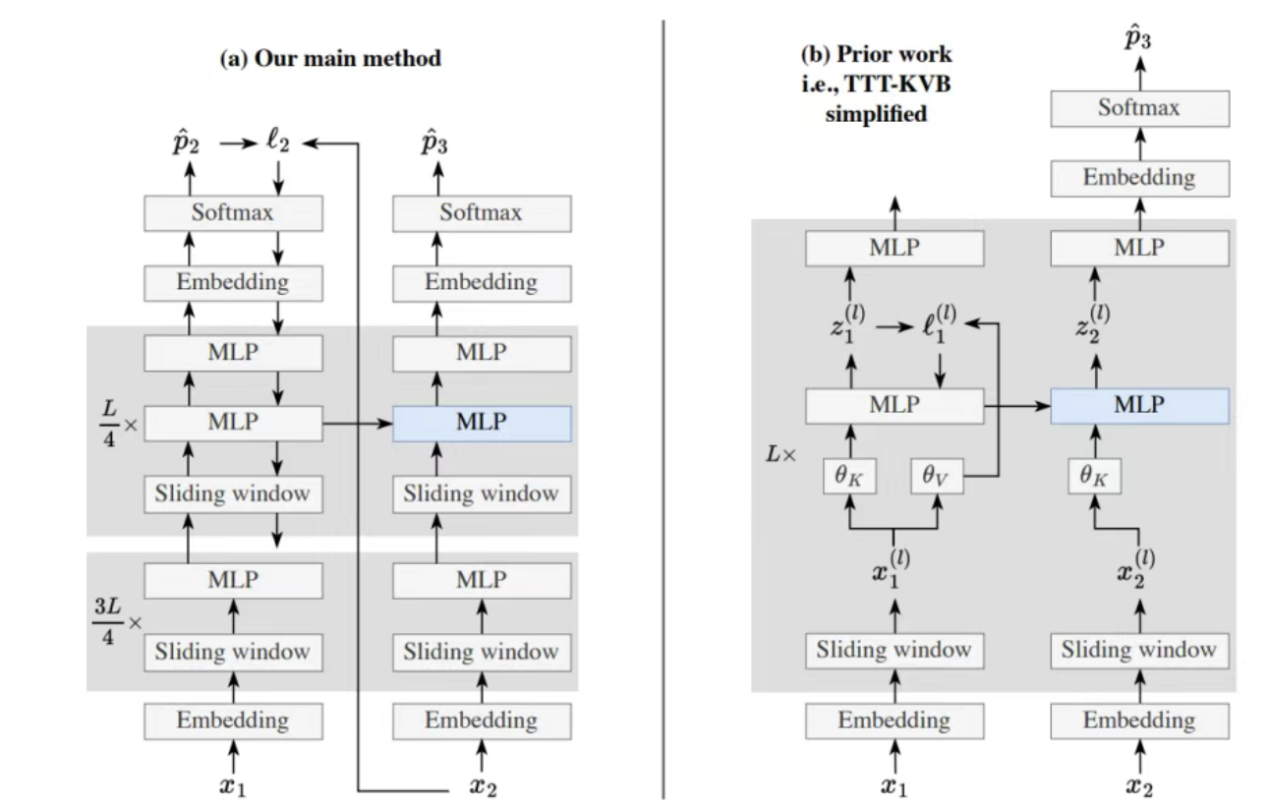
\includegraphics{images/image-0047.png}
\caption{TTT-E2E 与 TTT-KVB 的结构对比}
\end{figure}

\hypertarget{ux56dbux5982ux4f55ux907fux514dux5728ux663eux5b58ux4e2dux5b9eux4f8bux5316ux4e8cux9636hessianux77e9ux9635}{%
\subsubsection{（四）如何避免在显存中实例化二阶Hessian矩阵？}\label{ux56dbux5982ux4f55ux907fux514dux5728ux663eux5b58ux4e2dux5b9eux4f8bux5316ux4e8cux9636hessianux77e9ux9635}}

事实上，元学习的表达式中确实出现了二阶Hessian矩阵：

\[
\nabla_\theta J_{T_i}(\theta_i')
=
\nabla_{\theta_i'}J_{T_i}(\theta_i')
\cdot
\nabla_\theta\theta_i'
=
\nabla_{\theta_i'}J_{T_i}(\theta_i')
\cdot
\left(I+\alpha\nabla_\theta^2J_{T_i}(\theta)\right)
\]

但它是以和向量乘积的形式存在的，简化为考虑 Hessian 矩阵 \(H\) 和向量 \(v\) 乘积计算的问题：

\begin{enumerate}
\def\labelenumi{\arabic{enumi}.}
\tightlist
\item
  \textbf{计算一阶梯度}：对损失函数 \(\mathcal{L}\) 做一次常规反向传播，得到一阶梯度向量 \(g\)：
\end{enumerate}

\[
g=\nabla_\theta \mathcal{L}(\theta)
\]

此时显存开销为 \(O(N)\)，即存储梯度向量的大小。

\begin{enumerate}
\def\labelenumi{\arabic{enumi}.}
\setcounter{enumi}{1}
\tightlist
\item
  \textbf{构造标量点积}：将梯度向量 \(g\) 与目标向量 \(v\) 点积，得到纯标量：
\end{enumerate}

\[
S=g^\top v
\]

\begin{enumerate}
\def\labelenumi{\arabic{enumi}.}
\setcounter{enumi}{2}
\tightlist
\item
  \textbf{对标量求一阶导数}：对标量 \(S\) 再关于参数 \(\theta\) 求梯度：
\end{enumerate}

\[
\nabla_\theta S
= \nabla_\theta(g^\top v)
= (\nabla_\theta g)^\top v
= H v
\]

这一步实质上是在第一次反向传播建立的计算图上，再进行一次反向传播（reverse-over-reverse autodiff），显存开销仍保持在 \(O(N)\)。

这样的计算总开销约等于两次独立的前向+反向传播。

\hypertarget{ux4e94ux6838ux5fc3ux8ba1ux7b97ux5f00ux9500}{%
\subsubsection{（五）核心计算开销}\label{ux4e94ux6838ux5fc3ux8ba1ux7b97ux5f00ux9500}}

虽然单个时间步避免了 \(O(N^2)\) 的显存操作，但在 TTT-E2E 架构中，系统必须在长达数十万的 token 序列上展开计算图，这仍然引出了另一个维度的灾难。

\begin{enumerate}
\def\labelenumi{\arabic{enumi}.}
\tightlist
\item
  \textbf{随时间反向传播（BPTT）的状态膨胀}：
  在传统 RNN 或全注意力 Transformer 中，计算图随时间展开时，隐状态数量会随着序列长度线性增长。但在 TTT-E2E 的内层循环中，模型是将自身参数矩阵 \(W\) 作为随着时间演进的``隐状态''来进行持续学习，其内层更新规则类似于：
\end{enumerate}

\[
W_i = W_{i-1} - \eta\nabla_W l_i(W_{i-1})
\]

外层循环要计算 \(\nabla_{W_0}\mathcal{L}\)，必须穿过所有时间步反向传播：

\[
\frac{\partial\mathcal{L}}{\partial W_0}
=
\sum_i
\frac{\partial l_i}{\partial W_{i-1}}
\left(
\prod_{j=1}^{i-1}
\frac{\partial W_j}{\partial W_{j-1}}
\right)
\]

假设内层更新的 mini-batch 大小为 \(\hat b=1K\)，处理 \(T=128K\) 的上下文时，模型实际上要在内层循环中连续走 \(128\) 步梯度下降。

\begin{enumerate}
\def\labelenumi{\arabic{enumi}.}
\setcounter{enumi}{1}
\item
  \textbf{致命的显存耗尽（OOM）}：
  为了在反向传播时能计算上述梯度，前向传播必须在显存中保留所有中间状态。在 TTT 中，这意味着超长序列内每个下文切片都要形成一个巨大的权重链 \(W_1,W_2,\ldots,W_T\)，全部塞进显存。若不保存大部分中间权重，则反向传播时又需要重新计算，时间开销很大。
\item
  \textbf{``用时间换空间''的工程妥协：梯度检查点}：
  工程中可以用梯度检查点（Gradient Checkpointing）减少显存，但仍需要保存较多关键节点，并在反向传播时重新计算前向传播。对于 128K 级别的长上下文，这种方法仍会导致极高的时间成本。
\end{enumerate}

\hypertarget{ux516dux5173ux4e8emoe}{%
\subsubsection{（六）关于MoE}\label{ux516dux5173ux4e8emoe}}

正如前面所讨论的，TTT-E2E 能高效运行的核心在于把 1K 个 token 打包成一个 mini-batch，利用静态 MLP 计算统一的梯度 \(l_t(W)\) 并一次性更新。如果换成 MoE，这 \(1024\) 个 token 会被路由网络分配到不同专家：

\begin{itemize}
\tightlist
\item
  专家 A 可能只收到了 \(150\) 个 token 的梯度。
\item
  专家 B 可能收到了 \(300\) 个 token 的梯度。
\end{itemize}

底层 CUDA 算子无法对这些极其不规则的张量做 coalesced memory access，内存访问、线程排队、负载均衡都会变得困难。

MoE 的核心是门控（Gating）和路由网络，通常使用 Top-K 选择。这是一个不可导或至少高度非线性的过程。如果要在训练期让梯度穿过 TTT 更新步骤，再穿过 MoE 路由机制，其二阶导数的计算会变得不稳定，极易导致梯度爆炸或消失，模型根本无法收敛。

如果我们在架构设计上进行妥协，TTT-E2E 和 MoE 也并非完全不可结合。在 TTT-E2E 的官方实现中，为了保证速度，网络前 \(3/4\) 的层是\textbf{完全冻结（Frozen）}的，只有最后 \(1/4\) 的层参与 TTT 梯度更新。因此可行的折中方案是：

\begin{itemize}
\tightlist
\item
  \textbf{前 \(3/4\) 的冻结层使用 MoE 架构}：在这里发挥 MoE 的特长，用极低推理算力调用海量参数。
\item
  \textbf{后 \(1/4\) 的 TTT 层使用稠密（Dense）标准 MLP}：在这里保持规则的 dense 矩阵结构，使 TTT 更新具备高吞吐和稳定性。
\end{itemize}

\hypertarget{ux4e03ux5173ux4e8eux63a8ux7406ux548cagentux80fdux529b}{%
\subsubsection{（七）关于推理和Agent能力}\label{ux4e03ux5173ux4e8eux63a8ux7406ux548cagentux80fdux529b}}

Next-token prediction本质上是一种无监督的行为克隆。如果在测试时，强行让模型去拟合一段带有噪声、逻辑跳跃或次优决策的外部Context，确实极易引发``灾难性遗忘''，破坏掉前期通过PPO、GRPO等强化学习算法精调出的长链条推理和任务执行策略。

一种方法时让模型在测试时不去拟合外部给定的 Prompt，而是先利用现有的RL能力生成（或基于其他方法搜索出）高质量的推理步骤，然后结合环境反馈或验证对其经过筛选，利用经过筛选和重述的自身高质量数据来进行对前文所述的MLP模块的TTT更新，这就更类似于后面会提到的自蒸馏方法。

\hypertarget{ux4e8cin-place-ttt}{%
\subsection{二、In-Place TTT}\label{ux4e8cin-place-ttt}}

\hypertarget{ux4e00ux73b0ux6709ux6d4bux8bd5ux65f6ux8badux7ec3tttux65b9ux6cd5ux7684ux95eeux9898}{%
\subsubsection{（一）现有测试时训练（TTT）方法的问题}\label{ux4e00ux73b0ux6709ux6d4bux8bd5ux65f6ux8badux7ec3tttux65b9ux6cd5ux7684ux95eeux9898}}

\begin{enumerate}
\def\labelenumi{\arabic{enumi}.}
\item
  架构不兼容：现有TTT方法往往需要设计全新的独立层来替代自注意力机制，这意味着必须从头开始进行高昂的预训练，无法直接利用现有的模型。
\item
  计算效率低下：传统的TTT需要逐个Token顺序更新状态，严重限制了现代GPU/TPU的并行计算吞吐量。
\item
  目标不契合：以往TTT的自监督目标通常是简单的``重建当前词''，这与自回归语言模型``预测下一个词''的终极目标不一致。
\end{enumerate}

\hypertarget{ux4e8cux6838ux5fc3ux67b6ux6784-2}{%
\subsubsection{（二）核心架构}\label{ux4e8cux6838ux5fc3ux67b6ux6784-2}}

为解决上述问题，字节Seed提出了In-Place Test-Time Training框架。该框架不引入全新的网络层，而是直接将Transformer架构中普遍存在的MLP块中的最后一个投影矩阵 \(W_{\mathrm{down}}\) 征用为``快速权重''。这种``即插即用''的设计无需修改原始架构，保留了预训练权重的完整性，仅需极低的成本进行持续微调即可生效。

由于该方法作用于MLP层并与注意力机制互补，它允许以较大的分块为单位进行并行更新，极大地提升了在现代硬件上的吞吐量。

\hypertarget{ux4e09ux635fux5931ux51fdux6570}{%
\subsubsection{（三）损失函数}\label{ux4e09ux635fux5931ux51fdux6570}}

作者通过以下公式构造了一个带有``未来信息''的目标值 \(\hat V\)：

\[
V = \mathrm{Conv1D}(X_0)W_{\mathrm{target}}
\]

\begin{itemize}
\tightlist
\item
  \(X_0\) 是输入 token 最原始的词嵌入向量。
\item
  \(\mathrm{Conv1D}(\cdot)\) 是一个一维卷积。它以 3 层引入``未来信息''的核心机制，通过控制卷积核的权重，可以像滑动窗口一样把后面的词拉取过来。
\item
  \(W_{\mathrm{target}}\) 是一个可训练的矩阵，负责将卷积提取到的未来特征映射到合适的维度空间。
\end{itemize}

简单来说，我们希望神经网络最后一层的输出接近这个 \(V\) 值。神经网络最后一层的输出是上一层激活值 \(Z\) 经过权重 \(W_{\mathrm{down}}\) 后得到的。这里预测的词可以是上下文中的任何词，无论由用户、环境输入还是模型生成。

计算损失函数的过程如下：

\begin{enumerate}
\def\labelenumi{\arabic{enumi}.}
\tightlist
\item
  \textbf{计算当前输出}：模型使用当前的快速权重 \(W_{\mathrm{down}}^{(i)}\) 来处理当前激活值 \(Z_{[i]}\)，得到输出结果 \(O_{[i]}\)：
\end{enumerate}

\[
O_{[i]} = Z_{[i]}\left(W_{\mathrm{down}}^{(i)}\right)^T
\]

\begin{enumerate}
\def\labelenumi{\arabic{enumi}.}
\setcounter{enumi}{1}
\tightlist
\item
  \textbf{生成对齐目标}：模型利用 \(W_{\mathrm{target}}\) 计算出包含未来信息的标准答案 \(\hat V_{[i]}\)。
\item
  \textbf{计算损失并更新}：论文定义损失函数为两者之间的负内积：
\end{enumerate}

\[
\mathcal{L}=-\langle O_{[i]},\hat V_{[i]}\rangle_F
=
-\left\langle Z_{[i]}\left(W_{\mathrm{down}}^{(i)}\right)^T,\hat V_{[i]}\right\rangle_F
\]

最小化该负损失等价于最大化 \(Z_{[i]}(W_{\mathrm{down}})^\top\) 与 \(\hat V_{[i]}\) 之间的相似度。经过 \(W_{\mathrm{down}}\) 投影出来的结果如果能够与包含未来预测信息的 \(\hat V\) 高度对齐，说明该更新方向有效。

该方法采用极简的一阶更新。因为使用了最简单的内积作为损失函数，它的梯度推导清晰，快速权重更新为：

\[
W_{\mathrm{down}}^{(i)}
=
W_{\mathrm{down}}^{(i-1)}
+ \eta \hat V_{[i]}^\top Z_{[i]}
\]

为了防止 token 越来越多导致权重数值无界增长，论文还引入了 Frobenius 范数裁剪：

\[
\Delta W_{\mathrm{down}}^{(i)}
\leftarrow
\frac{\Delta W_{\mathrm{down}}^{(i)}}{\|\Delta W_{\mathrm{down}}^{(i)}\|_F}
\]

拓展：为什么不用交叉熵？

\begin{enumerate}
\def\labelenumi{\arabic{enumi}.}
\tightlist
\item
  Softmax的计算开销
\end{enumerate}

交叉熵路径中，模型必须把当前 \(d_{\mathrm{model}}\) 维隐状态映射到整个词表空间，词表大小可能达到 \(50K\) 到 \(150K\)。然后执行 Softmax、计算概率分布、求出误差，再反向传播穿过 LM Head 回到 MLP 层。TTT 的现实环境通常是推理阶段动态运行，如果每处理一个 chunk 都要做一次词表级别的反向传播，计算开销和显存占用都非常高。

\begin{enumerate}
\def\labelenumi{\arabic{enumi}.}
\setcounter{enumi}{1}
\tightlist
\item
  梯度公式简洁，易于优化
\end{enumerate}

如果采用非线性 Softmax 产生的高维非线性梯度，需要依赖深度学习框架进行 Top-K 内的大段反向图推导。而内积损失 \(C=-(ZW_{\mathrm{down}}^\top)\hat V^\top\) 的梯度对 \(W_{\mathrm{down}}\) 只有极其简单的解析解，避免了大规模反向图的维护和计算。

\begin{enumerate}
\def\labelenumi{\arabic{enumi}.}
\setcounter{enumi}{2}
\tightlist
\item
  上下文并行的要求
\end{enumerate}

为了实现计算加速，引入了上下文并行机制，利用并行扫描（Parallel Scan / Prefix Sum）来同时处理多个文本块。交叉熵的依赖链中，每一个 token 的分类都需要经过庞大的词表块，而内积损失对每个块而言只依赖于局部的 \(Z\)、目标 \(\hat V\) 和快速权重，梯度天然可以用矩阵加法/乘法组合，从而更容易并行化。

\hypertarget{ux56dbux4e3aux4ec0ux4e48ux5bf9ux63a8ux7406ux80fdux529bux7684ux5f71ux54cdux4e0dux5927}{%
\subsubsection{（四）为什么对推理能力的影响不大？}\label{ux56dbux4e3aux4ec0ux4e48ux5bf9ux63a8ux7406ux80fdux529bux7684ux5f71ux54cdux4e0dux5927}}

\begin{enumerate}
\def\labelenumi{\arabic{enumi}.}
\tightlist
\item
  架构层面
\end{enumerate}

In-Place TTT 并没有更新模型所有权重，而是做了一个非常精妙的隔离设计：

\begin{itemize}
\tightlist
\item
  \textbf{冻结``通用推理基座''}：模型的核心自注意力机制，以及 MLP 中间的 \(W_{\mathrm{up}}\) 和 \(W_{\mathrm{gate}}\) 都被完全冻结。作为``慢权重（Slow Weights）''保留了预训练阶段学到的常识逻辑和 agent 规划能力。
\item
  \textbf{只更新残差连接的一部分}：它仅将 MLP 的最后一个投影矩阵 \(W_{\mathrm{down}}\) 作为可热插拔更新模块。快速权重发生改变时，它实际上是在模型原有大推理路径之上做局部增量特征叠加：
\end{itemize}

\[
H_{\mathrm{out}} = H_{\mathrm{in}} + \mathrm{MLP}(H_{\mathrm{in}})
\]

当 \(W_{\mathrm{down}}\) 发生改变时，它主要是在原有完整推理路径之上增加一段局部记忆增强，不会破坏底层推理能力。

\begin{enumerate}
\def\labelenumi{\arabic{enumi}.}
\setcounter{enumi}{1}
\tightlist
\item
  目标函数层面
\end{enumerate}

论文指出，在实际工程实现中，这个目标函数并没有局限于单一的下一个 token。

\begin{itemize}
\tightlist
\item
  \textbf{局部未来特征的融合}：通过一维卷积 Conv1D 和映射矩阵 \(W_{\mathrm{target}}\) 的可学习组合，目标值 \(\hat V\) 实际上捕获的是一个局部未来 token 组合信息。
\item
  \textbf{与 MTP 思想相似}：这种设计与多 token 预测思路一致。强制模型在隐空间内一次性预测未来的多个演化状态，不仅不会削弱，反而会促进模型进行更深层的前向隐式规划。
\end{itemize}

\hypertarget{ux4e94ux9884ux586bux5145ux9636ux6bb5ux7684ux52a0ux901fux673aux5236ux56e0ux679cux586bux5145}{%
\subsubsection{（五）预填充阶段的加速机制：因果填充}\label{ux4e94ux9884ux586bux5145ux9636ux6bb5ux7684ux52a0ux901fux673aux5236ux56e0ux679cux586bux5145}}

在Agent任务中，模型需要在预填充阶段从长上下文中学习。

为了在预填充阶段进行高效训练，In-Place TTT 采用上下文并行（Context Parallelism），将极长的序列切分为多个块（chunk），并让所有 chunk 同时进行各自参数更新量 \(\Delta W\)。

这带来一个严重问题：理论上论文是为了``预测未来词''，如果在计算 chunk \(i\) 最后一个 token 的目标值 \(\hat V\) 时，卷积很有可能看到了哪怕一个未来的词，它就会跨界提取到 chunk \(i+1\) 的数据。这样就违反了跨块的数据依赖，chunk \(i\) 必须等待 chunk \(i+1\) 的数据，并行扫描算法的基石就会崩塌。

为确保对 chunk \(i\) 的更新量完全不包含未来的信息，作者在生成目标值时对 1D 卷积强行应用了因果填充：

\begin{itemize}
\tightlist
\item
  \textbf{常规卷积的视野}：如果卷积核大小为 \(5\)（即 \(K=5\)），为了计算位置 \(t\) 的特征，通常会取 \([t-2,t-1,t,t+1,t+2]\)，这显然包含了未来的信息。
\item
  \textbf{因果填充的具体做法}：实现中采用了核大小为 \(5\) 且带有因果填充的深度一维卷积。它会在序列左侧手动填充 \(4\) 个 \(0\)。这样一来，在计算位置 \(t\) 的特征时，感受野会变为 \([t-4,t-3,t-2,t-1,t]\)。
\end{itemize}

通过这种单向约束，每个 chunk 的计算被严格隔离在自己的边界内。这种局部机制使得高度并行的扫描算法在数学上完全等价于严格的因果序列过程。

当然，解码阶段仍然逐词串行输出和更新权重：

\begin{itemize}
\tightlist
\item
  \textbf{Apply}：模型直接使用当前维持的 \(W_{\mathrm{down}}\) 对这个 token 进行投影，得到输出。
\item
  \textbf{Update}：计算这个 token 带来的较小梯度增量 \(\Delta W\)，并将其累加到 \(W_{\mathrm{down}}\) 中。在这个过程中同样受到很小阈值 \(\tau=10^{-5}\) 的强制裁断保护，防止持续累积退化。
\end{itemize}

\hypertarget{ux53c2ux8003ux6587ux732e-148}{%
\subsection{参考文献}\label{ux53c2ux8003ux6587ux732e-148}}

\begin{itemize}
\tightlist
\item
  Tandon, A., Dalal, K., Li, X., et al.~(2025). \href{https://arxiv.org/abs/2512.23675}{End-to-End Test-Time Training for Long Context}. arXiv:2512.23675.
\item
  Feng, G., Luo, S., Hua, K., et al.~(2026). \href{https://arxiv.org/abs/2604.06169}{In-Place Test-Time Training}. arXiv:2604.06169.
\end{itemize}

\clearpage

\hypertarget{titansux4e0enested-learningux8bbaux6587}{%
\section{Titans与Nested Learning（论文）}\label{titansux4e0enested-learningux8bbaux6587}}

\begin{quote}
本文是论文阅读笔记，内容代表对应论文方法或作者理解，不应直接视为领域共识或工程最佳实践。
\end{quote}

\hypertarget{ux4e00titans}{%
\subsection{一、Titans}\label{ux4e00titans}}

Google Research提出的Titans将模型视为一个具有不同层次记忆系统的智能体，通过对Delta Attention进行泛化，引入了一种能够在测试时改变权重、进行记忆的长短期神经记忆模块。

\hypertarget{ux4e00ux6838ux5fc3ux601dux60f3-14}{%
\subsubsection{（一）核心思想}\label{ux4e00ux6838ux5fc3ux601dux60f3-14}}

Titans架构由三个相互关联的Hyper-heads组成，模拟了人类大脑处理信息的不同方式：

Transformer模块：类似于人类的短期记忆（工作记忆），负责处理当前数据流，通常使用窗口有限的注意力机制实现。

长期记忆模块：类似于人类的长期记忆，维护大小恒定的MLP，在推理过程中通过梯度下降不断更新其中的参数，从而``存储''长期的历史信息。

静态参数模块：训练后``冻结''的参数，存储全局知识和能力。

\hypertarget{ux4e8cux957fux671fux8bb0ux5fc6ux6a21ux5757ux7684ux57faux672cux539fux7406}{%
\subsubsection{（二）长期记忆模块的基本原理}\label{ux4e8cux957fux671fux8bb0ux5fc6ux6a21ux5757ux7684ux57faux672cux539fux7406}}

和Kimi Delta Attention类似，计算新信息的Key经过记忆模块后的输出与Value之间的误差，作为``惊讶度''，损失函数为：

\[
\mathcal{L}_{\Delta} = \frac{1}{2}\left\|S^\top k_t - v_t\right\|_2^2
\]

即梯度更新的幅度与误差成正比，误差大意味着过往信息中没有这部分内容，记忆模块通过梯度更新将其``记住''。

但Titans也作出了改进和泛化：

\begin{enumerate}
\def\labelenumi{\arabic{enumi}.}
\item
  将单一矩阵（线性层）改为MLP，包含了非线性激活函数。多层 MLP 的非线性表达能力远强于线性矩阵，能把更复杂的历史抽象压缩进参数里。
\item
  采用了动量法，原来的 MLP 为 \(\mathcal{M}_{t-1}\) 时，利用梯度的移动平均 \(S_t\) 更新 MLP 的参数：
\end{enumerate}

\[
\mathcal{M}_t = \mathcal{M}_{t-1} - \eta \nabla \mathcal{L}(\mathcal{M}_{t-1})
\]

这样可以增加前后token之间语境的连贯性。

需要注意的是，对于第 \(t\) 个输入 token（或段落，段落中的 token 并行经过记忆模块和推理，此时记忆模块记录上一段落及更早的记忆，即每段只用和原来之间的平均损失更新一次）检索时，输出一个由和输入段落同样多的 embedding 向量构成的序列（矩阵）：

\[
h_t = \mathcal{M}^{*}_{t-1}(q_t)
\]

上面所述的更新过程均发生在这步计算完成之后，因为记忆模块的目的是``检索过去的信息''，不能让本token的Key和Value混入其中影响判断。

\hypertarget{ux4e09ux8bb0ux5fc6ux6a21ux5757ux878dux5165ux6a21ux578bux67b6ux6784ux7684ux65b9ux5f0f}{%
\subsubsection{（三）记忆模块融入模型架构的方式}\label{ux4e09ux8bb0ux5fc6ux6a21ux5757ux878dux5165ux6a21ux578bux67b6ux6784ux7684ux65b9ux5f0f}}

Memory As a Context：将记忆检索结果作为上下文拼接，在处理长程依赖时表现最好。

Memory As a Gate：记忆与注意力分支并行并门控融合。

Memory As a Layer：记忆模块作为独立层顺序堆叠。效率最高但性能较差。这种顺序设计限制了模型同时利用注意力和神经记忆互补处理数据的能力，但优势在于能更好地适配FlashAttention等硬件加速技术。

\hypertarget{ux56dbux4e3aux4ec0ux4e48titansux65e0ux6cd5ux50cfkimi-delta-attentionux90a3ux6837ux8fc5ux901fux6295ux5165ux4e1aux754cux5e94ux7528}{%
\subsubsection{（四）为什么Titans无法像Kimi Delta Attention那样迅速投入业界应用？}\label{ux56dbux4e3aux4ec0ux4e48titansux65e0ux6cd5ux50cfkimi-delta-attentionux90a3ux6837ux8fc5ux901fux6295ux5165ux4e1aux754cux5e94ux7528}}

\begin{enumerate}
\def\labelenumi{\arabic{enumi}.}
\tightlist
\item
  必须保留计算图和显式执行反向传播
\end{enumerate}

核心在于上述的梯度表达式。Kimi Delta Attention之所以不需要显式执行反向传播，是因为其隐状态更新公式可直接求出解析解，通过矩阵乘法和加法来更新隐状态：

\[
\mathcal{M}_t = (1 - \alpha_t)\mathcal{M}_{t-1} + S_t
\]

\[
S_t = \eta_t S_{t-1} - \theta_t \nabla \mathcal{L}(\mathcal{M}_{t-1}; x_t)
\]

从而我们不需要保留计算图。

但是Titans存在非线性激活函数，其梯度在跨越激活函数的过程中，无法简单地写成解析闭式解，因此在推理更新阶段，系统必须维护一个针对该MLP模块的局部计算图来执行梯度下降，还要保留优化器状态。这带来了巨大的计算开销，和现在业界的推理优化方式不兼容。

【注意】Titans在训练时直接舍弃二阶梯度项，即训练时直接由L对``当前时刻的瞬时权重''求梯度。主要计算开销在于推理时的反向传播。

\begin{enumerate}
\def\labelenumi{\arabic{enumi}.}
\setcounter{enumi}{1}
\tightlist
\item
  Memory as a Context和Memory As a Gate无法用Flash Attention大规模并行
\end{enumerate}

我们知道，当输入第 \(t\) 个 token（或段落，段落中的 token 并行经过记忆模块和推理，此时记忆模块记录上一段落及更早的记忆，即每段只用和原来之间的平均损失更新一次）时，会先经过记忆模块：

\[
S_t = S_{t-1} + \beta_t k_t \left(v_t^\top - k_t^\top S_{t-1}\right)
\]

随后记忆模块更新：

\[
\mathcal{M}_t = (1 - \alpha_t)\mathcal{M}_{t-1} + S_t
\]

\[
S_t = \eta_t S_{t-1} - \theta_t \nabla \mathcal{L}(\mathcal{M}_{t-1}; x_t)
\]

MAC：处理第 2 段 \(q_2\)（\(x_2\)）就必须要先算出整个 \(\mathcal{M}_1\)，\(\mathcal{M}_1\) 需要通过 \(x_1\) 的值由梯度下降（无法写成显式解，即矩阵加法和乘法形式）才得到，必须一步一步串行。Flash Attention能在同一段上下文内部执行分块加速，但它无法跨段落融合。因为在算子层面，全局计算图被``权重更新''这一步骤物理性地切断了。

MAG：注意力分支中，对于一篇文章的各个段落（从1到t）可以完美使用Flash Attention。然而，由于最终输出需要注意力输出与记忆输出在每一位置进行门控融合，这限制了某些深度端到端的内核优化，因为数据必须从SRAM回写到HBM进行融合。

MAL：当所有段落都经过记忆层后，就完全同步了，可以直接用Flash Attention对整个文本的计算进行分块加速。

\hypertarget{ux4e94ux4e3aux4ec0ux4e48titansux5f3aux4e8eux7528ragux6ce8ux5165ux4e0aux4e0bux6587}{%
\subsubsection{（五）为什么Titans强于用RAG注入上下文？}\label{ux4e94ux4e3aux4ec0ux4e48titansux5f3aux4e8eux7528ragux6ce8ux5165ux4e0aux4e0bux6587}}

\begin{enumerate}
\def\labelenumi{\arabic{enumi}.}
\item
  压缩和抽象：简单地将文本块存入文件系统或向量数据库，检索出来的是原始数据。原始数据往往包含大量噪声，且没有经过``理解''和``压缩''。而Titans长期记忆模块通过梯度下降学习的是数据的抽象，它将成千上万个token的逻辑关系``浓缩''进神经网络的参数中。
\item
  ``惊讶度''驱动：只有当输入的信息违反了模型的预期（即很``令人惊讶''）时，模型才会产生强烈的梯度去大幅修改权重。这种机制让模型能自主决定哪些信息是真正值得``刻骨铭心''的，哪些只是重复的废话。
\item
  表达能力：大多数外置记忆检索基于线性相似度，且把序列切成块存进文件系统，块与块之间的逻辑流动会断裂；Titans使用深度（≥2层）MLP，且运用动量法使得前后token更连贯。
\item
  解决``迷失在中间''和窗口限制：RAG 提取回来的上下文依然受限于Transformer的窗口大小，且模型往往会产生``迷失在中间''的现象，无法有效利用极长的上下文；Titans是在参数层面更新，可以轻松扩展到更长的上下文窗口，而传统的检索或简单的循环模型此时性能会剧烈下滑。
\end{enumerate}

\hypertarget{ux516dux8badux7ec3ux65f6ux4e00ux9636ux9012ux5f52ux7684ux65f6ux95f4ux590dux6742ux5ea6}{%
\subsubsection{（六）训练时一阶递归的时间复杂度}\label{ux516dux8badux7ec3ux65f6ux4e00ux9636ux9012ux5f52ux7684ux65f6ux95f4ux590dux6742ux5ea6}}

在同一个块内，通过固定初始权重，可以一次性并行算出所有 token 的梯度项总和，时间复杂度为 \(O(1)\)。而在不同块间，训练时利用 \(S_0\) 算出 \(S_N\) 的时间复杂度是 \(O(\log N)\) 而非 \(O(N)\)。关键在于下一段对上一段的依赖关系可以写成一阶仿射递推。

Titans 中的动量项可以抽象为：

\[
S_t = \eta_t S_{t-1} + u'_t
\]

其中 \(u'_t=-\theta_t\nabla\mathcal{L}\)，即当前块带来的梯度更新项。进一步抽象为：

\[
S_t = a_t S_{t-1}+b_t
\]

其中 \(a_t=\eta_t\)，\(b_t=u'_t\)。若以二次损失为例，记忆矩阵也可写成同类线性变换：

\[
\mathcal{M}_t
=
\mathcal{M}_{t-1}(I-2\eta k_tk_t^\top)
 + 2\eta v_tk_t^\top
\]

也就是说，和Kimi Delta Attention一样，上式可看成对上一时刻记忆模块的线性变换。定义一个元组算子：

\[
\mathcal{T}_t=(a_t,b_t)
\]

它表示从状态 \(t-1\) 到状态 \(t\) 的转换。若有连续的两个转换 \(\mathcal{T}_1=(a_1,b_1)\) 与 \(\mathcal{T}_2=(a_2,b_2)\)，则合成后：

\[
S_2 = a_2(a_1S_0+b_1)+b_2
= (a_2a_1)S_0+(a_2b_1+b_2)
\]

利用 \(S_0\) 算出 \(S_2\)，只需要经过两个算子的融合：

\[
\mathcal{T}_{1:2}=(a_2a_1,\;a_2b_1+b_2)
\]

这种算子组合满足结合律：

\[
(\mathcal{T}_1\oplus\mathcal{T}_2)\oplus\mathcal{T}_3
=
\mathcal{T}_1\oplus(\mathcal{T}_2\oplus\mathcal{T}_3)
\]

由于满足结合律，就可以做并行扫描：

\begin{enumerate}
\def\labelenumi{\arabic{enumi}.}
\tightlist
\item
  第一层并行计算 \((1\oplus2)\)、\((3\oplus4)\)、\((5\oplus6)\ldots\)，每个单位时间消耗 1 个时间步。
\item
  第二层并行合并更长片段，得到 \((1-4)\)、\((5-8)\ldots\)。
\item
  对数层级地合并，经过 \(\log_2 N\) 次合并后即可得到从起始点到任意位置 \(t\) 的总转换算子。
\end{enumerate}

\hypertarget{ux4e8cnested-learning}{%
\subsection{二、Nested Learning}\label{ux4e8cnested-learning}}

\hypertarget{ux4e00ux95eeux9898ux80ccux666f-3}{%
\subsubsection{（一）问题背景}\label{ux4e00ux95eeux9898ux80ccux666f-3}}

无论是训练MLP还是运行Linear Attention，都可以被写成同一个通用的联想记忆优化目标：

\[
\mathcal{M}_{new}
=
\arg\min_{\mathcal{M}}
\mathrm{Mapping}(\mathrm{Key}, \mathrm{Value})
 + \mathrm{Regularization}
\]

MLP 训练是在低频（整个预训练数据集上、只训练一次）求解一个优化问题，将``输入 \(x\)''映射到``梯度信号 \(u\)''；Attention 推理是在高频（当前上下文窗口内、每次输入 token 时）求解一个优化问题，将``Key''线性回归映射到``Value''。也就是说，MLP的``训练''和 Attention 的``推理''，在数学形式上是完全一样的（都是在做梯度下降），区别仅仅在于它们的更新频率和数据来源不同。

现在的Transformer，本质是在外层MLP内部嵌入一个Attention层。进一步说，Transformer 实际上是一组并行的、频率不同的线性层，有的线性层（MLP）更新得很慢（由于预训练），有的线性层（Attention）更新得极快（在推理时实时更新）。

外层是一个极低频优化的MLP，它在预训练时注入通用知识，并永久记忆，但无法更新（更新频率为0）；内层则是一个高频优化的线性回归，它（在任务结束前）每输入一个token就更新（更新频率极高），但难以记忆（大模型在上下文处理时的``灾难性遗忘''）。于是我们想到两个改进：

\begin{enumerate}
\def\labelenumi{\arabic{enumi}.}
\item
  线性回归毕竟比较弱，能不能把内部换成高频优化的MLP呢？
\item
  能否找一个中等的优化（更新）频率，作为外层与内层之间的``中间层''，隔一定量的token更新一次，既能更新知识，又不至于因过快更新导致遗忘，从而解决LLM在预训练结束后就无法学习新知识的问题？
\end{enumerate}

（注：我们这里假设模型``在线学习''，即相当于Transformer中的前向推理过程一直不结束，模型持续学习新知识，不会出现KV Cache中的``清空显存''操作）

\hypertarget{ux4e8chopeux67b6ux6784}{%
\subsubsection{（二）HOPE架构}\label{ux4e8chopeux67b6ux6784}}

结合上面所述，我们参考大脑中不同频率的电波，构造以下HOPE架构：

\[
y_t =
\mathrm{MLP}^{(f_k)}
\bigl(
\cdots
\mathrm{MLP}^{(f_1)}(x_t)
\cdots
\bigr)
\qquad (30)
\]

参数更新规则为：

\[
\theta^{(f_l)}_{i+1}
=
\theta^{(f_l)}_{i}
-
\sum_{t=i-C^{(l)}}^{i}
\eta_t^{(l)}
f\!\left(\theta_t^{(f_l)};x_t\right),
\quad
\text{if } i\equiv 0\pmod{C^{(l)}}
\qquad (31)
\]

其中：

\begin{itemize}
\tightlist
\item
  \textbf{高频层（类似海马体）}：记录改变自己的结构参数，捕捉当前的对话细节、临时人名或数字。如果这层参数不更新，模型就会忘记前一句话说了什么。
\item
  \textbf{中频层（类似皮层整合）}：它的参数变化较慢，负责提取经常出现的主题、逻辑流。它忽略短枝末节，只记住``大概发生了什么''。
\item
  \textbf{低频层（类似长期知识）}：极其稳定，几乎不怎么变，存储核心语言规则和世界知识。
\end{itemize}

在 HOPE 架构中，前向计算过程包含了一个\textbf{在线更新步骤}。这意味着，虽然网络经过预训练后有固定参数，但当前上下文仍会通过某些局部目标改变其中一部分参数。

HOPE 的局部目标可以写为：

\[
W_{t+1}
=
\arg\min_W
\left\|
W x_t - \nabla_{y_t}\mathcal{L}(W_t;x_t)
\right\|_2^2
\]

它不是让模型简单地输出 \(y=Wx\)，而是要求当前输入 \(x_t\) 经过更新后的权重 \(W_{t+1}\) 后，能够生成一个接近误差信号或``惊讶信号''的输出。这类似于把``当前样本告诉我的更新方向''写入权重。

\hypertarget{ux4e09ux4f18ux5316ux5668ux9009ux62e9}{%
\subsubsection{（三）优化器选择}\label{ux4e09ux4f18ux5316ux5668ux9009ux62e9}}

尽管如前面所述，我们可以训练一个神经网络作为优化器，但在 HOPE 架构中，每一层 MLP（即连续体记忆系统中的每一块）使用的是一种基于L2回归目标的改进型梯度下降优化器：

\[
W_{t+1}
=
W_t(I-x_tx_t^\top)
-
\eta_{t+1}\nabla_W\mathcal{L}(W_t;x_t)\otimes x_t
\]

展开来看：

\begin{itemize}
\tightlist
\item
  \textbf{衰减/去相关项 \(W_t(I-x_tx_t^\top)\)}：这一项源于 \(L_2\) 回归目标对模长的惩罚。它会清除 \(W_t\) 中与当前输入 \(x_t\) 方向一致的旧分量，从而防止由于数据相关性导致的权重累积或爆炸。
\item
  \textbf{学习/写入项 \(-\eta_{t+1}\nabla_W\mathcal{L}(W_t;x_t)\otimes x_t\)}：这是标准梯度下降项，负责把新的误差信号写入权重。
\end{itemize}

该公式等价于求解以下局部优化问题：

\[
\min_W
\left\|
W x_t - \nabla_{y_t}\mathcal{L}(W_t;x_t)
\right\|_2^2
\]

这里的目标是找到一个 \(W\)，使其对当前输入 \(x_t\) 的预测输出尽可能接近当前的局部惊讶信号或梯度信号。

\begin{enumerate}
\def\labelenumi{\arabic{enumi}.}
\tightlist
\item
  为什么用基于L2回归目标的优化器，不用向量点积相似度？
\end{enumerate}

在向量检索（Retrieval）或静态特征比对中，我们通常更喜欢点积或余弦相似度；HOPE架构的优化场景（即在线更新参数）中，逻辑却不同，正是为了抑制``模长噪声''和``冗余信号''，才需要切换回L2回归。

\begin{itemize}
\tightlist
\item
  \textbf{检索场景（Retrieval）}：只需要找相似问题。如果向量 \(A\) 模长很大，它可能会在欧氏距离上远离目标，但在角度上很近。因此 Cosine/Dot Product 忽略模长是合理的。
\item
  \textbf{优化场景（Optimization, HOPE）}：要优化权重矩阵 \(W\)。如果只关注方向，\(W\) 的模长可能无限增大；而 L2 回归会同时惩罚方向错误和模长错误，避免权重沿相关数据方向失控。
\item
  \textbf{在线数据相关性}：离线训练依赖 shuffle 和 batching，样本近似 i.i.d.；在线或嵌套学习中，\(x_t\) 与 \(x_{t+1}\) 往往高度相关。此时 \((I-xx^\top)\) 项能把已经写入的相关分量消掉，避免连续相似样本把同一方向无限放大。
\end{itemize}

拓展：在工程实践中，为什么这种权重模长失控的情况很少出现？

\begin{itemize}
\tightlist
\item
  \textbf{权重衰减（Weight Decay / L2 Regularization）}：AdamW 或 SGD 通常会设置 \texttt{weight\_decay} 参数：
\end{itemize}

\[
\mathcal{L}_{total}
=
\mathcal{L}_{task}
+ \lambda\|W\|^2
\]

这会在梯度中引入 \(-2\lambda W\) 项，持续把 \(W\) 的模长向下拉。

\begin{itemize}
\tightlist
\item
  \textbf{该论文的观点}：论文通过 L2 回归目标推导出的公式，本质上把``如果我们用正确的数学目标，这件事就天然发生''说明出来。工程中的 \texttt{weight\_decay} 是这个思想的近似版本。
\item
  \textbf{自适应学习率（Adam）}：Adam 会除以梯度二阶矩的平方根 \(\sqrt{v_t}\)。如果某一维在同一方向积累导致数值变大，\(v_t\) 也会变大，从而自动降低学习率。这本质上是一种数值缓冲机制。
\end{itemize}

\begin{enumerate}
\def\labelenumi{\arabic{enumi}.}
\setcounter{enumi}{1}
\tightlist
\item
  为什么Linear Attention中，我们推导出解析解就是 \(VK^\top\)，这里却不能用？
\end{enumerate}

在矩阵形式下，严格的最小二乘解析解应为：

\[
M^* = VK^\dagger
=
VK^\top(KK^\top)^{-1}
\]

\begin{itemize}
\tightlist
\item
  \textbf{解析真相}：数学告诉我们理想解应包含 \((KK^\top)^{-1}\)，即协方差矩阵的逆。它负责去相关（de-correlation）。
\item
  \textbf{Hebbian / Attention 假设}：如果 \(K\) 是正交的，那么 \(KK^\top=I\)，此时解析解简化为 \(M^*=VK^\top\)。
\item
  \textbf{线性注意力做法}：直接计算 \(\sum vk^\top\)。它假设所有 \(k\) 都是独立的，不需要计算那个昂贵的逆矩阵。
\item
  \textbf{Delta Rule / HOPE 假设}：Key 或 token embedding 高度相关，\(KK^\top\neq I\)。因此简单 \(VK^\top\) 会重复计算相似特征。Delta Rule 使用残差更新：
\end{itemize}

\[
\Delta M = (v-Mk)k^\top
\]

它只更新当前矩阵还没有预测准确的差异部分，更接近逐步逼近真正最小二乘解的过程。

换言之，Linear Attention 更像一个``纯粹的记账器''，它假设数据正交，直接把 \(v\) 贴在 \(k\) 上；HOPE/Delta Rule 更像在线回归器，它每次根据误差修正已有权重，最终效果更接近 \(VK^\dagger\)。

\hypertarget{ux53c2ux8003ux6587ux732e-149}{%
\subsection{参考文献}\label{ux53c2ux8003ux6587ux732e-149}}

\begin{itemize}
\tightlist
\item
  Behrouz, A., Zhong, P., \& Mirrokni, V. (2024). \href{https://arxiv.org/abs/2501.00663}{Titans: Learning to Memorize at Test Time}. arXiv:2501.00663.
\item
  Behrouz, A., Razaviyayn, M., Zhong, P., \& Mirrokni, V. (2025). \href{https://arxiv.org/abs/2512.24695}{Nested Learning: The Illusion of Deep Learning Architectures}. arXiv:2512.24695.
\end{itemize}

\clearpage

\hypertarget{ux65c1ux8defux5faeux8c03ux8bbaux6587}{%
\section{旁路微调（论文）}\label{ux65c1ux8defux5faeux8c03ux8bbaux6587}}

\begin{quote}
本文是论文阅读笔记，内容代表对应论文方法或作者理解，不应直接视为领域共识或工程最佳实践。
\end{quote}

在测试时学习中，为了避免``灾难性遗忘''，我们希望尽量不改变主模型的参数，避免摧毁训练阶段获得的知识和能力。由此，可以用一个旁路模块实现长期记忆。

\hypertarget{ux4e00ux5229ux7528lora}{%
\subsection{一、利用LoRA}\label{ux4e00ux5229ux7528lora}}

LoRA是一种经典的微调方法，两个低秩参数矩阵相乘再和主模型参数相加。改变只发生在这两个低秩矩阵构成的向量空间，对主模型影响不大。但这样的缺点在于，低秩参数矩阵自身能``容纳''的正交基向量极少，不同记忆难以正交存储，容易发生冲突，导致实际有效记忆量非常有限。

在Test-Time Training的框架下，为当前测试样本计算出的LoRA模块必须在任务（或该样本的推理）结束后立刻清零。当然，也有LoRA Hub等复用LoRA的方法：在不同的任务上训练出不同独立的LoRA，构成LoRA库，运行一个新任务时用特征检索的方法挑选出若干个最符合情境的LoRA挂载使用：

\textbf{特征入库（Key 生成）}：当系统使用某个 LoRA 适配器完成一个任务后，会用 Embedding 模型 \(E\) 对该任务的原始指令或 Prompt \(x_{\mathrm{task}}\) 提取特征向量，将其作为该 LoRA 的静态身份键：

\[
k_i = E(x_{\mathrm{task}})
\]

随后把 \(k_i\) 与 LoRA 权重一并落盘。这个过程在历史任务完成后发生。

\textbf{测试时路由（Query 匹配）}：当遇到新的测试输入 \(x_{\mathrm{new}}\) 时，在前向传播的早期用同一个 Embedding 模型提取查询向量：

\[
v_q = E(x_{\mathrm{new}})
\]

动态门控值计算（Gating）：所有历史 LoRA 的键向量 \(k_i\) 与 \(v_q\) 做余弦相似度匹配，并加上温度系数 \(\tau\) 的 Softmax，得到每个 LoRA 应被采用的路由权重：

\[
g_i =
\frac{\exp(\cos(v_q,k_i)/\tau)}
{\sum_{j=1}^{N}\exp(\cos(v_q,k_j)/\tau)}
\]

如果采用 \textbf{Weight-Level Routing（权重级合并）}，系统会选择 Top-K 相似的 LoRA（如 \(K=3\)），直接用算出的相似度权重 \(g_i\) 对这些 LoRA 的降维矩阵 \(A_i\) 和升维矩阵 \(B_i\) 加权求和，生成一个新的临时适配器：

\[
\Delta W_{\mathrm{merged}} =
\sum_{i\in \mathrm{TopK}} g_i(A_iB_i)
\]

如果采用 \textbf{Activation-Level Routing（激活级专家 MoE）}，每个 LoRA 会保持独立的前向旁路，让大模型每一层的隐藏状态 \(h_{\mathrm{in}}\) 分别通过不同的 LoRA，再将输出按门控权重聚合：

\[
h_{\mathrm{out}} =
h_{\mathrm{in}} +
\sum_{i\in \mathrm{TopK}} g_i \cdot \mathrm{LoRA}_i(h_{\mathrm{in}})
\]

如果纯余弦相似度无法捕捉任务间的隐式组合关系，可能用一个带参数的路由层，此时可能可以在测试时的空闲时段（类似于人的睡眠时间）冻结主模型参数，训练LoRA路由等。

\hypertarget{ux4e8clocaslocally-supported-parametric-memory}{%
\subsection{二、Locas（Locally-Supported Parametric Memory）}\label{ux4e8clocaslocally-supported-parametric-memory}}

\hypertarget{ux4e00ux53ccux5c42ffnux4e0eux56faux5b9akvux7684ux6ce8ux610fux529bux67e5ux627eux8868ux7684ux7b49ux4ef7ux6027}{%
\subsubsection{（一）双层FFN与固定KV的注意力、查找表的等价性}\label{ux4e00ux53ccux5c42ffnux4e0eux56faux5b9akvux7684ux6ce8ux610fux529bux67e5ux627eux8868ux7684ux7b49ux4ef7ux6027}}

在经典 Transformer 架构中，带有非线性激活函数 \(\phi(\cdot)\) 的两层 FFN 标准矩阵运算可写为：

\[
\mathrm{FFN}(A_i^l)=V^T\phi(K^T A_i^l)
\]

其中：

\begin{itemize}
\tightlist
\item
  \(A_i^l \in \mathbb{R}^d\) 是在第 \(i\) 层、第 \(t\) 个 token 位置输入到 FFN 的激活特征向量。
\item
  \(K\in \mathbb{R}^{d\times m}\) 是第一层权重矩阵，在该框架下可被视为``键矩阵''（Key Matrix）。
\item
  \(V\in \mathbb{R}^{m\times d}\) 是第二层权重矩阵，可被视为``值矩阵''（Value Matrix）。
\item
  \(m\) 是 FFN 的中间维度，通常远大于隐藏维度 \(d\)。
\end{itemize}

由此我们看出，两层FFN可以看成一个K、V固定的注意力层。当特征向量（Query）进入，可以起到查询记忆的作用：

\begin{enumerate}
\def\labelenumi{\arabic{enumi}.}
\tightlist
\item
  \textbf{模式匹配（Query 与 Key 的交互）}：
  输入 \(A_i^l\) 可以看作查询向量（Query）。键向量 \(k_j\) 充当一个特定的``特征模式探测器''。内积 \(\langle A_i^l,k_j\rangle\) 衡量了当前输入特征与第 \(j\) 个记忆槽中预存模式的匹配程度或相似度。
\item
  \textbf{门控激活（Activation）}：
  非线性函数 \(\phi(\cdot)\)（如 ReLU 或 SiLU）在这里扮演``激活门''的角色。如果匹配程度低于某个阈值，\(\phi\) 会输出 \(0\) 或极小的值，意味着该记忆槽保持静默；如果匹配程度高，则输出一个正向的标量权重，使该记忆槽具有被激活的特性。
\item
  \textbf{内容提取（Value）}：
  值向量 \(v_j\) 代表第 \(j\) 个记忆槽中实际存储的知识内容或输出贡献。
\item
  \textbf{加权聚合（Weighted Sum）}：
  最终求和操作会把所有被成功激活的记忆槽中的内容 \(v_j\)，按模式匹配强度的权重 \(\phi(\langle A_i^l,k_j\rangle)\) 线性叠加，汇聚成这一层最终输出的特征表示。
\end{enumerate}

在这个视角下，FFN 的中间维度 \(m\) 直接代表了模型拥有的记忆槽数量（Memory Capacity）。如果我们在测试阶段动态增加一个或多个局部记忆槽，并让它们与原有 FFN 架构兼容，就可在不需要存放或微调原有矩阵 \((k_j,v_j)\) 的情况下实现参数化记忆。

我们只需要在求和公式中新增一项，即增加一个维度 \(m+1\)，并在其中写入精心初始化的键值对 \((k_{m+1},v_{m+1})\)。这就是 Locas 提出``旁路（Sideway）FFN''架构的根本依据：它通过在数学原理上等效地扩充 \(m\)，实现了纯粹的参数化记忆扩容，同时物理隔离了新旧知识，避免了灾难性遗忘。

Locas的本质，就是通过算法（例如激活引导的主成分分析或梯度更新），将原本冗长、占据海量显存的KV Cache中的知识提取、压缩并蒸馏到了这几个新增的参数化记忆槽中。

\hypertarget{ux4e8cux521dux59cbux5316ux65b9ux6cd5}{%
\subsubsection{（二）初始化方法}\label{ux4e8cux521dux59cbux5316ux65b9ux6cd5}}

为了避免主模型被随机写入噪声，Locas-GLU 实体的初始化策略遵循一个极度严谨的物理原则：在初始化的第一刻，新模块对主干网络输出的物理影响必须为零，但其内部特征探测器必须处于高度敏感的``热启动''状态。

具体工作流如下：

\begin{enumerate}
\def\labelenumi{\arabic{enumi}.}
\tightlist
\item
  \textbf{预评估与特征嗅探（寻找主导激活子空间）}：
  在正式写入测试时间训练前，给定一段输入文本块 \(x_t\)，模型首先执行一次纯粹的前向传播。在这个过程中，算法会监控并记录主干网络 GLU-FFN 层中所有中间维度的激活状态 \(M_i^l\)：
\end{enumerate}

\[
a_j^l = \frac{1}{T}\sum_{t=1}^{T}\left|M_{t,j}^l\right|
\]

随后，算法计算每个维度在整个时间步 \(T\) 上的平均绝对激活强度 \(a_j^l\)。

\begin{enumerate}
\def\labelenumi{\arabic{enumi}.}
\setcounter{enumi}{1}
\tightlist
\item
  \textbf{非线性 PCA 与参数克隆（构建``热启动''探测器）}：
  根据算出的激活强度 \(a_j^l\) 排序，算法会精准地挑出最活跃的 Top-\(r\) 个维度，其中 \(r\) 为 Locas 的极小 rank 值，如 \(64\)。这相当于在激活空间做一次非线性主成分分析（PCA）。接着，算法直接从主干网络的权重矩阵中，把这 \(r\) 个最关键的行向量克隆出来，并归一化，作为 Locas 层的键矩阵 \(K^i\) 和门矩阵 \(G^i\) 的初始值：
\end{enumerate}

\[
K^i \leftarrow \mathrm{Normalize}(W_K^i|_{c_j:s})
\]

\[
G^i \leftarrow \mathrm{Normalize}(W_G^i|_{c_j:s})
\]

这一步并没有存入新的上下文记忆。它的目的是为旁路模块建立一套对当前上下文极其敏感的``专属雷达系统''。因为这些参数已经经过了海量预训练，具有完美的非线性几何性质，这使得 Locas 模块瞬间拥有了很高的``阅读理解能力''，也就是论文中所说的``热启动（Warm Start）''。

\begin{enumerate}
\def\labelenumi{\arabic{enumi}.}
\setcounter{enumi}{2}
\tightlist
\item
  \textbf{零状态守卫（切断初始噪声的绝对物理隔离）}：
  这是避免噪声引入的最关键一步。尽管探测器 \(K\) 和 \(G\) 已经被完美初始化，但决定最终输出内容的值矩阵（Value Matrix）\(V\) 被强制初始化为全零矩阵。因为 \(V\) 是全零的，所以在初始化的第一步，无论输入特征如何激活 Locas 模块，其经过 \(V^T\) 投影后的输出永远是 \(0\)。主干网络接收到的附加信号为零，因此模型的原始行为在此时刻得到了 \(100\%\) 保留，没有任何噪声被注入。
\end{enumerate}

\hypertarget{ux4e09ux66f4ux65b0ux65b9ux6cd5}{%
\subsubsection{（三）更新方法}\label{ux4e09ux66f4ux65b0ux65b9ux6cd5}}

实际操作中，我们无法像前面说的那样``每进来一个token就增加一对(k,v)''，只能固定若干个（如64个）槽位，用梯度下降的方式更新参数（当然也可以每进来一个token就增加一对(k,v)，然后达到上限后用一些数学技巧压缩，但那样计算开销大大增加且效果无提升）。这里的槽位不需要像KV Cache那么多，因为KV Cache中必须一个位置对应一个token，即便两个token意思完全相同也必须按顺序分开存储，而这里只要保证有足够的维度来存储信息。在一个任务中，有用的信息往往分布在低维流形上，故槽位数并不需要非常多。

完成``热启动''和``零状态守卫''后，模型开始处理流式长文本。此时，参数的更新完全依赖于标准的反向传播机制，但范围被严格限制：

\begin{enumerate}
\def\labelenumi{\arabic{enumi}.}
\tightlist
\item
  \textbf{冻结主干，放开旁路}：整个预训练大模型的数亿或数百亿参数被冻结，梯度不回传给它们。只有 Locas 层的极少量参数 \((K,G,V)\) 开始接收梯度。
\item
  \textbf{语言建模目标驱动}：随着模型不断进行 Next-Token Prediction（基于流式上下文 \(x_{<t}\) 预测下一个词 \(x_t\)），系统计算标准的交叉熵损失，即对数似然 \(\log p(x_t\mid x_{<t})\)。
\item
  \textbf{梯度微调}：由于目标函数的梯度会反向传播流经整个计算图，直接影响到 Locas 层时，原本为 \(0\) 的值矩阵 \(V\) 会根据当前的误差信号获得一个非常小的梯度步进。
\item
  \textbf{持续烙印}：随着输入不断滑过，\(V\) 矩阵逐渐接收全局状态，开始针对特定上下文模式存储与之对应的``纠偏信号''或``事实知识''。因为 \(K\) 和 \(G\) 已经是主干激活特性的优秀子空间克隆，所以梯度的下降方向极其精准，通常只需要极少的步数就能快速收敛。
\end{enumerate}

\hypertarget{ux56dbux907fux514dux707eux96beux6027ux9057ux5fd8ux7684ux7ea6ux675fux673aux5236}{%
\subsubsection{（四）避免``灾难性遗忘''的约束机制}\label{ux56dbux907fux514dux707eux96beux6027ux9057ux5fd8ux7684ux7ea6ux675fux673aux5236}}

\begin{enumerate}
\def\labelenumi{\arabic{enumi}.}
\tightlist
\item
  \textbf{权重范数裁剪（Weight Norm Clipping）}：
  在每次推理时，对 \(K\)、\(G\)、\(V\) 矩阵中的每一个向量 \(w\) 强制执行裁剪：
\end{enumerate}

\[
w \leftarrow \frac{w}{\max(\|w\|_2,1)}
\]

这确保了记忆模块在每一步的贡献都不会限制在一个固定半径的超球体输出空间内，以较低的计算成本隐式地实现了对模型行为偏移的 KL 散度约束。

\begin{enumerate}
\def\labelenumi{\arabic{enumi}.}
\setcounter{enumi}{1}
\tightlist
\item
  \textbf{自适应输出缩放因子（Output Scaling Factor）}：
  Locas 的输出不是直接加回主干，而是乘上一个缩放因子 \(r\)：
\end{enumerate}

\[
\mathcal{H}_{\mathrm{out}} = \mathrm{FFN}(A) + r \cdot \mathrm{Locas\text{-}GLU}(A)
\]

其中 \(r\) 会被计算为主干网络向下投影矩阵的平均范数和记忆宽度，确保了即使记忆模块被完全激活，其输出的物理量级也不会超过主干网络的常规激活范围，构成了防止灾难性遗忘的双重保险。

\hypertarget{ux53c2ux8003ux6587ux732e-150}{%
\subsection{参考文献}\label{ux53c2ux8003ux6587ux732e-150}}

\begin{itemize}
\tightlist
\item
  Lu, S., Liang, Z., Ma, D., Wang, Y., Mi, H., \& Yu, D. (2026). \href{https://arxiv.org/abs/2602.05085}{Locas: Your Models are Principled Initializers of Locally-Supported Parametric Memories}. arXiv:2602.05085.
\item
  Zhao, Z., Gan, L., Wang, G., et al.~(2024). \href{https://arxiv.org/abs/2402.09997}{LoraRetriever: Input-Aware LoRA Retrieval and Composition for Mixed Tasks in the Wild}. Findings of ACL 2024.
\item
  Zhao, Z., Gan, L., Wang, G., et al.~(2024). \href{https://arxiv.org/abs/2406.16989}{Retrieval-Augmented Mixture of LoRA Experts for Uploadable Machine Learning}. arXiv:2406.16989.
\item
  Huang, C., Liu, Q., Lin, B. Y., Pang, T., Du, C., \& Lin, M. (2023). \href{https://arxiv.org/abs/2307.13269}{LoraHub: Efficient Cross-Task Generalization via Dynamic LoRA Composition}. COLM 2024.
\item
  Gandelsman, Y., Sun, Y., Chen, X., \& Efros, A. A. (2022). \href{https://arxiv.org/abs/2209.07522}{Test-Time Training with Masked Autoencoders}. NeurIPS 2022.
\end{itemize}

\clearpage

\hypertarget{openclaw-rlux4e2aux4ebaagentux7684ux6301ux7eedux5b66ux4e60ux8bbaux6587}{%
\section{OpenClaw-RL：个人Agent的持续学习（论文）}\label{openclaw-rlux4e2aux4ebaagentux7684ux6301ux7eedux5b66ux4e60ux8bbaux6587}}

\begin{quote}
本文是论文阅读笔记，内容代表对应论文方法或作者理解，不应直接视为领域共识或工程最佳实践。
\end{quote}

\hypertarget{ux4e00ux6838ux5fc3ux601dux60f3-15}{%
\subsection{一、核心思想}\label{ux4e00ux6838ux5fc3ux601dux60f3-15}}

现有的智能体 RL 系统通常忽略了交互后产生的\textbf{下一状态信号（next-state signals）}，例如用户的回复、工具输出、环境的状态变化等，仅将其作为生成下一步动作的上下文。这种做法无法有效了解和利用有价值的在线反馈信息被浪费：

\begin{itemize}
\tightlist
\item
  \textbf{评估性信号（Evaluative signals）}：下一状态隐式地对前一个动作进行了质量打分。例如，用户对智能体重新提问代表不满意，测试用例通过代表成功，而代码报错代表失败。
\item
  \textbf{指导性信号（Directive signals）}：除了单纯的打分，下一状态通常还会具体指出修改建议。例如，详细的错误日志、或者用户直接指出``你应该先检查文件再修改''，这些 token 级别提供了明确的定向优化信号。
\end{itemize}

\hypertarget{ux4e8cux7cfbux7edfux67b6ux6784}{%
\subsection{二、系统架构}\label{ux4e8cux7cfbux7edfux67b6ux6784}}

为了实现在线、实时的训练并避免单点阻塞，OpenClaw-RL 基于异步框架构建了\textbf{完全解耦（fully decoupled）}的系统架构。它包含四个独立运行的异步循环：

\begin{enumerate}
\def\labelenumi{\arabic{enumi}.}
\tightlist
\item
  \textbf{策略服务（Policy Serving）}：由 SGLang 驱动，负责不同场景、不同用户请求或环境交互的在线推理服务。
\item
  \textbf{环境服务器（Environment Servers）}：对于个人智能体，环境即用户的本地设备，通过加密 API 与 RL 服务器通信；对于通用智能体，环境部署在云服务上以支持大规模并行计算。
\item
  \textbf{奖励裁判（Reward Judging）}：利用 SGLang 或 API 部署过程奖励模型（PRM），对收集到的历史交互进行分步或整段文本提示。
\item
  \textbf{策略训练（Policy Training）}：由 Megatron 引擎负责，在后台处理样本队列并进行模型权重的平滑更新（graceful weight update），全程不会中断前端的推理服务。
\end{enumerate}

\hypertarget{ux4e09ux6838ux5fc3ux7b97ux6cd5}{%
\subsection{三、核心算法}\label{ux4e09ux6838ux5fc3ux7b97ux6cd5}}

\hypertarget{ux4e00ux9488ux5bf9ux8bc4ux4f30ux6027ux4fe1ux53f7ux7684ux4e8cux8fdbux5236ux5f3aux5316ux5b66ux4e60}{%
\subsubsection{（一）针对评估性信号的二进制强化学习}\label{ux4e00ux9488ux5bf9ux8bc4ux4f30ux6027ux4fe1ux53f7ux7684ux4e8cux8fdbux5236ux5f3aux5316ux5b66ux4e60}}

该方法将评估信号转化为二值奖励，并用强化学习更新策略：

\begin{enumerate}
\def\labelenumi{\arabic{enumi}.}
\tightlist
\item
  \textbf{工作流}：

  \begin{itemize}
  \tightlist
  \item
    智能体在状态 \(s_t\) 下生成响应动作 \(a_t\)。
  \item
    环境或用户反馈产生下一状态 \(s_{t+1}\)。
  \item
    系统调用 PRM 模型，依据 \(s_{t+1}\) 到 \(a_t\) 的质量进行评估，输出初步分数 \(r_t\)。
  \item
    通过多数投票（majority vote）或规则化的最终判断，把反馈转化为 \(0/1\) 奖励。
  \item
    直接把最终奖励作为该步的优势函数 \(A_t=r_{\mathrm{final}}\)，并将其送入训练队列。
  \end{itemize}
\item
  \textbf{数学公式}：
  该方法采用标准的带有非对称裁剪的 PPO 代理目标函数：
\end{enumerate}

\[
\begin{aligned}
L_{\mathrm{PPO}}
&=
-\mathbb{E}_t
\left[
\min\left(
\rho_t A_t,
\mathrm{clip}(\rho_t,1-\epsilon,1+\epsilon_{\mathrm{high}})A_t
\right)
\right]
\end{aligned}
\]

其中，\(\rho_t=\frac{\pi_\theta(a_t\mid s_t)}{\pi_{\mathrm{old}}(a_t\mid s_t)}\) 是新旧策略的概率比率。

\hypertarget{ux4e8cux9488ux5bf9ux5f15ux5bfcux6027ux4fe1ux53f7ux7684ux84b8ux998f}{%
\subsubsection{（二）针对引导性信号的蒸馏}\label{ux4e8cux9488ux5bf9ux5f15ux5bfcux6027ux4fe1ux53f7ux7684ux84b8ux998f}}

该方法将包含丰富纠错信息的指导性信号，转化为 token 级别的定向监督信号。

\begin{enumerate}
\def\labelenumi{\arabic{enumi}.}
\tightlist
\item
  \textbf{工作流}：

  \begin{itemize}
  \tightlist
  \item
    \textbf{提取提示（Hindsight Hint Extraction）}：教师模型对 \(s_t\) 和 \(s_{t+1}\) 进行分析，如果观察到动作的优化建议，即提取为一个提示 \(h\)，如果没有则返回 \(h=\varnothing\)。
  \item
    \textbf{过滤与选择（Quality Filtering）}：为了保证训练信号的纯度，系统会过滤掉无效样本；在多个有效 hint 中，选择长度最长、信息量最大的一个。
  \item
    \textbf{构建增强上下文（Enhanced Teacher Construction）}：将提取出的 hint 以特定格式（如 \texttt{{[}User\textquotesingle{}s\ hint\ /\ instruction{]}\textbackslash{}n{[}hint{]}}）附加到上一步的系统上下文中，构造出一个包含了``事后诸葛亮''信息的增强状态 \(s_{\mathrm{enhanced}}\)。
  \item
    \textbf{计算 token 级别优势}：让策略模型在原始状态 \(s_t\) 和增强状态 \(s_{\mathrm{enhanced}}\) 下分别计算原动作 \(a_t\) 中每个 token 的对数概率，并求差值。
  \end{itemize}
\item
  \textbf{数学公式}：
  token 级别的优势计算公式为：
\end{enumerate}

\[
\begin{aligned}
A_t
&=
\log \pi_{\mathrm{teacher}}(a_t\mid s_{\mathrm{enhanced}})
-\log \pi_\theta(a_t\mid s_t)
\end{aligned}
\]

这里是在比较学生上下文和教师上下文下生成学生动作的概率，只是评价学生模型生成的token的好坏，并没有让教师生成新token并进行KL散度损失计算。这和在线自蒸馏并不一样。

为什么 \(A_t\) 取这个值：

在深度学习中，让学生模型 \(\pi_\theta\) 去学习教师模型 \(\pi_{\mathrm{teacher}}\) 的行为，最标准的方法是最小化它们分布之间的 KL 散度：

如果我们对 KL 散度求梯度，即我们要更新学生模型参数 \(\theta\) 的方向，其核心可以近似推导为：

\[
\begin{aligned}
\nabla_\theta D_{\mathrm{KL}}(\pi_\theta\Vert\pi)
&\approx
-\left(
\log \pi_{\mathrm{teacher}}(a_t)
-\log \pi_\theta(a_t)
\right)
\nabla_\theta \log \pi_\theta(a_t)
\end{aligned}
\]

现在再看强化学习。标准的策略梯度（Policy Gradient）算法更新参数 \(\theta\) 的基本公式是：

\[
\begin{aligned}
\nabla_\theta L_{\mathrm{PG}}
&= -A_t \cdot \nabla_\theta \log \pi_\theta(a_t)
\end{aligned}
\]

两式对应即得。值得注意的是，真实的 KL 散度梯度含有期望项，但是在实际的大模型工程中，对每个步骤都计算全词表的期望会导致计算量爆炸。考虑到 \(a_t\) 就是我们在这一步由学生模型策略真实采样生成的 Token，所以 \(a_t\) 本身就可以作为这个期望的一个无偏估计量。

大语言模型的最后一层是没有被归一化的分数，即 logits。当我们使用 Softmax 函数把 logits 转化为概率时：

\[
P(z_i)=\frac{e^{\mathrm{logit}_i}}{\sum_j e^{\mathrm{logit}_j}}
\]

对其取对数：

\[
\log P(z_i)=\mathrm{logit}_i-\log\left(\sum_j e^{\mathrm{logit}_j}\right)
\]

可以看到，对数概率本质上就是模型输出的 logit 值减去一个常数归一项。因此，logit 越高，模型生成该 token 的倾向越强；反向传播会把优势 \(A_t\) 作用到对应 token 的 logit 上。

\hypertarget{ux4e09ux8054ux5408ux4f18ux5316}{%
\subsubsection{（三）联合优化}\label{ux4e09ux8054ux5408ux4f18ux5316}}

Binary RL 能够覆盖所有带有评分的交互轮次，而 OPD 能够在用户或环境给出明确指导时提供高分辨率的逐 token 纠正。由于两者共享相同的 PPO 损失函数架构，论文提出通过直接加权两者的优势函数来进行联合优化：

\[
\begin{aligned}
A_t
&=
\omega_{\mathrm{binary}} r_{\mathrm{final}}
\\
&\quad+
\omega_{\mathrm{opd}}
\left(
\log \pi_{\mathrm{teacher}}(a_t\mid s_{\mathrm{enhanced}})
-\log \pi_\theta(a_t\mid s_t)
\right)
\end{aligned}
\]

其中，\(\omega_{\mathrm{binary}}\) 与 \(\omega_{\mathrm{opd}}\) 用于控制终局评分与指导性蒸馏信号的相对权重。

\hypertarget{ux53c2ux8003ux6587ux732e-151}{%
\subsection{参考文献}\label{ux53c2ux8003ux6587ux732e-151}}

\begin{itemize}
\tightlist
\item
  OpenClaw. (2026). \href{https://github.com/openclaw/openclaw}{OpenClaw-RL project}.
\end{itemize}

\clearpage

\hypertarget{ux5229ux7528ux8d85ux7f51ux7edcux7684ux6301ux7eedloraux5faeux8c03ux8bbaux6587}{%
\section{利用超网络的持续LoRA微调（论文）}\label{ux5229ux7528ux8d85ux7f51ux7edcux7684ux6301ux7eedloraux5faeux8c03ux8bbaux6587}}

\begin{quote}
本文是论文阅读笔记，内容代表对应论文方法或作者理解，不应直接视为领域共识或工程最佳实践。
\end{quote}

\hypertarget{ux4e00ux6838ux5fc3ux601dux60f3-16}{%
\subsection{一、核心思想}\label{ux4e00ux6838ux5fc3ux601dux60f3-16}}

目前，为了让预训练的 LLM 适应特定的下游任务或新知识，业界通常采用两种范式：提示词工程（Prompt Engineering）和参数微调（如 SFT 或 LoRA）。但这两种方法均存在明显局限：

\begin{itemize}
\tightlist
\item
  \textbf{提示词工程}：将大量上下文塞入 Prompt 中会消耗宝贵的上下文窗口容量，并显著增加推理延迟。
\item
  \textbf{参数微调}：训练开销巨大，对超参数敏感，且需要为每一个特定任务保留一套独立的模型权重，造成巨大的存储负担。
\end{itemize}

``超网络（Hypernetwork）''作为一种生成另一个网络权重的特殊网络，为解决这一问题提供了理想方案：它有望通过一次前向计算直接生成任务所需的适配器参数。然而，LLM 参数空间极大，过去的超网络受限于架构瓶颈，始终无法成为 LLM 适配的实用且可扩展的解决方案。

具体来说，超网络的输入为模型输入，输出为LoRA模块的参数，即模型参数需要变化的量。

SHINE 的核心突破在于：\textbf{仅需单次前向传播，即可将复杂的、多样化的自然语言上下文，直接映射转化为高质量的 LLM LoRA 参数，全程无需任何基于梯度的微调训练。}

通过这种方法，输入文本的知识被瞬间``内化''到模型参数中，大模型随后即可基于这些注入的参数进行多轮问答或推理，无需在推理时再读取冗长的原始上下文。

\begin{itemize}
\tightlist
\item
  \textbf{复用 LLM 作为上下文编码器}：SHINE 没有从零开始训练一个庞大的外部编码器，而是直接内联使用了预训练 LLM 自身的参数来压缩文本。这意味着超网络直接继承了 LLM 的语言理解能力，免去了海量的基础训练开销。
\end{itemize}

\hypertarget{ux4e8cux6a21ux578bux67b6ux6784ux4e0eux5de5ux4f5cux6d41}{%
\subsection{二、模型架构与工作流}\label{ux4e8cux6a21ux578bux67b6ux6784ux4e0eux5de5ux4f5cux6d41}}

\hypertarget{ux4e00ux8bb0ux5fc6ux63d0ux53d6}{%
\subsubsection{（一）记忆提取}\label{ux4e00ux8bb0ux5fc6ux63d0ux53d6}}

\begin{enumerate}
\def\labelenumi{\arabic{enumi}.}
\tightlist
\item
  \textbf{输入拼接}：给定长度为 \(N\) 的上下文 token 嵌入 \(X\)，模型在其尾部追加一段长度为 \(M\) 的可学习初始化记忆嵌入序列 \(M_0\)。其拼接后的输入序列表示为：
\end{enumerate}

\[
h_0 = [X;M_0]\in\mathbb{R}^{(N+M)\times H}
\]

其中 \(H\) 是 LLM 的隐藏层维度。

\begin{itemize}
\tightlist
\item
  这个 \(M_0\) 是一组可学习的参数（Learnable Memory Embeddings）。
\item
  在超网络的元训练阶段，\(M_0\) 与 M2P Transformer 以及 Meta LoRA 的参数一起被梯度下降优化。
\item
  当训练完成进入推理阶段时，\(M_0\) 的数值就已经被完全固定下来。它就像一种特殊的``结构化 Prompt''，负责作为信息载体去吸收前文 \(X\) 的语义。
\end{itemize}

\begin{enumerate}
\def\labelenumi{\arabic{enumi}.}
\setcounter{enumi}{1}
\tightlist
\item
  \textbf{前向传播与提取}：LLM 处理上述拼接序列后，提取每一层（第 \(i\) 层）输出的最后 \(M\) 个 token 的隐藏状态作为该层的记忆状态 \(M_i\)：
\end{enumerate}

\[
M_i = h_i[N:N+M,:]\in\mathbb{R}^{M\times H}
\]

\begin{enumerate}
\def\labelenumi{\arabic{enumi}.}
\setcounter{enumi}{2}
\tightlist
\item
  \textbf{构建全局记忆张量}：将所有 \(L\) 层的 \(M_i\) 堆叠起来，形成一个全局记忆张量 \(M\)：
\end{enumerate}

\[
M=\mathrm{Stack}(M_1,\ldots,M_L)\in\mathbb{R}^{L\times M\times H}
\]

\begin{enumerate}
\def\labelenumi{\arabic{enumi}.}
\setcounter{enumi}{3}
\tightlist
\item
  \textbf{无瓶颈约束}：为了保证生成的参数有足够的信息容量，记忆序列的长度 \(M\) 必须满足能够容纳生成的 LoRA 权重。设生成的 LoRA 秩为 \(r\)，单层所有线性层的输入输出维度之和为 \(D_l\)，则强制约束：
\end{enumerate}

\[
M=\frac{rD_l}{H}
\]

这样就保证了记忆状态的尺寸至少等于 LoRA 参数的尺寸，从根本上消除了信息瓶颈。

\hypertarget{ux4e8cm2p-transformer}{%
\subsubsection{（二）M2P Transformer}\label{ux4e8cm2p-transformer}}

拿到全局记忆张量 \(M\) 后，需要将其转化为目标 LoRA 参数。如果直接把 \(M\) 展开为一个长度为 \(LMH\) 的序列并使用标准 Transformer 处理，自注意力计算复杂度将达到 \(O((LM)^2)\)，在计算上难以承受。因此，SHINE 引入了一个轻量级的稀疏注意力 M2P Transformer。

具体原理与工作流如下：

\begin{enumerate}
\def\labelenumi{\arabic{enumi}.}
\tightlist
\item
  \textbf{位置编码（Positional Encoding）}：为了让网络感知记忆状态所在的层级和 token 顺序结构，模型引入了可学习的层级位置嵌入 \(P_{\mathrm{layer}}\) 和 token 位置嵌入 \(P_{\mathrm{token}}\)：
\end{enumerate}

\[
\tilde{M}=M+P_{\mathrm{layer}}+P_{\mathrm{token}}
\]

\begin{enumerate}
\def\labelenumi{\arabic{enumi}.}
\setcounter{enumi}{1}
\tightlist
\item
  \textbf{稀疏交替自注意力（Sparse Alternating Attention）}：M2P Transformer 交替执行列注意力（层间）和行注意力（token 间），将时间复杂度降低到 \(O(LM^2+ML^2)\)。行注意力的计算可写为：
\end{enumerate}

\[
Y_{:,j}^{(l)}=\mathrm{SelfAttn}(Z_{:,j}^{(l)})
\]

这一步的理论意义极其关键：它允许信息在层与层之间双向流动，让深层特征能够传递回浅层。这在直觉上模仿了反向传播的过程，打破了传统基于隐藏状态逐层生成参数时的``盲目性''。

\begin{itemize}
\tightlist
\item
  \textbf{偶数层（行注意力 / 跨 token 混合）}：在同一层的不同 token 之间进行计算。
\end{itemize}

\hypertarget{ux4e09ux5229ux7528transformerux7684ux8f93ux51faux5f97ux5230loraux53c2ux6570}{%
\subsubsection{（三）利用Transformer的输出得到LoRA参数}\label{ux4e09ux5229ux7528transformerux7684ux8f93ux51faux5f97ux5230loraux53c2ux6570}}

把前面Transformer的输出按它所在的层重新分配，然后对每一层分别按如下步骤重新用LoRA：

\begin{enumerate}
\def\labelenumi{\arabic{enumi}.}
\tightlist
\item
  \textbf{展平为一维向量}：首先，将第 \(i\) 层对应的记忆切片 \(\tilde{M}_i\) 展开，形成一个非常长的一维向量 \(c\in\mathbb{R}^{M\cdot H}\)。可以把 \(c\) 想象成一条装满了几万个浮点数的长纸带。
\item
  \textbf{初始化指针}：设定一个游标指针 \(t\)，初始值为 \(0\)。它代表``我们当前在这条纸带上用到了哪个位置''。
\item
  \textbf{分配矩阵 \(A\)}：假设我们现在要为该层的第一个模块（例如 Query 投影层）生成输入维度为 \(I\)、秩为 \(r\) 的 LoRA 矩阵 \(A\)。这个矩阵需要 \(I\cdot r\) 个参数。算法从 \(c\) 的第 \(t\) 个位置开始，一直往后截取 \(I\cdot r\) 个元素：
\end{enumerate}

\[
c[t:t+I\cdot r]
\]

随后将这一维数组变形（reshape）成二维矩阵 \(A\in\mathbb{R}^{I\times r}\)。

\begin{enumerate}
\def\labelenumi{\arabic{enumi}.}
\setcounter{enumi}{3}
\tightlist
\item
  \textbf{分配矩阵 \(B\)}：接着为该模块生成矩阵 \(B\)，输出维度为 \(O\) 的 LoRA 矩阵 \(B\)。这个矩阵需要 \(r\cdot O\) 个参数。算法紧接着上一次截取结束的位置，从 \(c\) 中取出 \(r\cdot O\) 个元素：
\end{enumerate}

\[
c[t+I\cdot r:t+I\cdot r+r\cdot O]
\]

随后将该段数据变形为二维矩阵 \(B\in\mathbb{R}^{r\times O}\)。

\begin{enumerate}
\def\labelenumi{\arabic{enumi}.}
\setcounter{enumi}{4}
\tightlist
\item
  \textbf{更新指针}：生成完这一对 \(A\) 和 \(B\) 后，指针 \(t\) 前进 \(I\cdot r+r\cdot O\) 个数值，并继续为下一层或下一个模块取数。
\end{enumerate}

这样，此后模型前向传播时用的就是新权重了。

\hypertarget{ux56dbloraux662fux5426ux8de8ux4f1aux8bddux4fddux7559}{%
\subsubsection{（四）LoRA是否跨会话保留？}\label{ux56dbloraux662fux5426ux8de8ux4f1aux8bddux4fddux7559}}

不保留。SHINE 的核心理念是``即时调用''。它的工作流是针对给定的上下文（Context），通过单次前向传播生成一套对应的 LoRA 权重。记忆状态 \(M_i\) 是 LLM 结合当前输入的文本 \(X\) 和固定的 \(M_0\) 动态计算出来的隐状态。如果开启了一个全新的会话或输入了全新的上下文，模型会根据新的文本重新进行单次前向传播，生成全新的记忆状态和对应的 LoRA 参数，旧的记忆状态会被直接丢弃。

\hypertarget{ux4e09ux8badux7ec3ux65b9ux6cd5}{%
\subsection{三、训练方法}\label{ux4e09ux8badux7ec3ux65b9ux6cd5}}

\begin{itemize}
\tightlist
\item
  \textbf{阶段一：预训练（Pretraining）}：
  模型在无监督语料上进行自监督学习，包含两个主要任务：

  \begin{itemize}
  \tightlist
  \item
    \textbf{重建任务（Reconstruction）}：让超网络把完整文本编码进 LoRA，然后要求 LLM 仅依靠该 LoRA 来重构原始上下文。
  \item
    \textbf{补全任务（Completion）}：隐藏文本最后 \(10\%\) 到 \(30\%\) 的 token，要求生成的 LoRA 具备推理缺失信息的能力，从而让 LLM 补全残缺部分。
  \end{itemize}
\item
  \textbf{阶段二：指令微调（Instruction Fine-Tuning）}：
  利用构造的上下文-问答对数据集（如 MS MARCO MQA 等），计算预测答案 token 的交叉熵损失。这一阶段旨在赋予生成的 LoRA 理解、提炼复杂上下文并将其用于精准问答的能力。
\end{itemize}

\hypertarget{ux53c2ux8003ux6587ux732e-152}{%
\subsection{参考文献}\label{ux53c2ux8003ux6587ux732e-152}}

\begin{itemize}
\tightlist
\item
  Hu, E. J., Shen, Y., Wallis, P., et al.~(2022). \href{https://arxiv.org/abs/2106.09685}{LoRA: Low-Rank Adaptation of Large Language Models}. ICLR 2022.
\item
  Nguyen, T., Rosenberg, M., Song, X., et al.~(2016). \href{https://arxiv.org/abs/1611.09268}{MS MARCO: A Human Generated MAchine Reading COmprehension Dataset}. arXiv:1611.09268.
\item
  Liu, Y., Wang, X., Mao, Y., Gelberg, Y., Maron, H., \& Zhang, M. (2026). \href{https://arxiv.org/abs/2602.06358}{SHINE: A Scalable In-Context Hypernetwork for Mapping Context to LoRA in a Single Pass}. arXiv:2602.06358.
\item
  Anonymous. (2025). \href{https://arxiv.org/abs/2506.06105}{Text-to-LoRA: Instant Transformer Adaption}. ICML 2025.
\end{itemize}

\clearpage

\hypertarget{ux81eaux4e3bux5b66ux4e60ux7684ux667aux80fdux7cfbux7edfux5c55ux671bux8bbaux6587}{%
\section{自主学习的智能系统展望（论文）}\label{ux81eaux4e3bux5b66ux4e60ux7684ux667aux80fdux7cfbux7edfux5c55ux671bux8bbaux6587}}

\begin{quote}
本文是论文阅读笔记，内容代表对应论文方法或作者理解，不应直接视为领域共识或工程最佳实践。
\end{quote}

\hypertarget{ux4e00ux5f53ux524daiux7684ux95eeux9898}{%
\subsection{一、当前AI的问题}\label{ux4e00ux5f53ux524daiux7684ux95eeux9898}}

\textbf{学习过程的外包}：当前的 AI 模型（如大语言模型）一旦部署，其内部的运行模式便固定下来，本质上无法在真实交互中持续学习新知识。它们的学习过程完全被外包给了人类专家：在被称为 MLOps 的流程中，人类负责收集和清洗数据、调整损失函数、制定严格的训练配方（例如先进行海量自监督预训练，再辅以人类反馈强化学习）。

\textbf{领域不匹配（Domain Mismatch）}：因为 AI 的优化是在固定的训练数据分布上进行的，当系统被部署到复杂的现实世界中，面对重启分布的新奇事件或随时间变化的非平稳动态时，其表现会产生不可预测的灾难性下滑。这与生物有机体利用自身环境中的可用数据进行原位适应、快速应对生态位变化的能力形成了鲜明对比。

Yann LeCun等提出了一套受人类和动物认知启发的学习架构，整合了基于观察的学习（System A）和基于主动行为的学习（System B），并能够根据内部生成的元控制信号在这些学习模式之间灵活切换。

\hypertarget{ux4e8ca-b-mux81eaux4e3bux5b66ux4e60ux67b6ux6784}{%
\subsection{二、A-B-M自主学习架构}\label{ux4e8ca-b-mux81eaux4e3bux5b66ux4e60ux67b6ux6784}}

\textbf{System A：基于观察的学习（Learning from Observation）}

System A 代表了一种被动接收并处理感觉输入的统计或预测机制。在 AI 中，这类算法的典型代表是自监督学习（SSL）或语言建模。\textbf{核心功能}是通过被动观察世界，提取数据的统计分布，抽象出从低级感官特征到高级概念的潜在表征，并构建能够预测未来的``世界模型''。

\begin{itemize}
\tightlist
\item
  \textbf{工作流与数学原理}：

  \begin{enumerate}
  \def\labelenumi{\arabic{enumi}.}
  \tightlist
  \item
    环境数据从分布 \(D\) 中采样，即 \(x\sim D\)。
  \item
    任务生成器 \(G\) 会从原始样本 \(x\) 中生成用于训练的输入与预测目标的配对：
  \end{enumerate}
\end{itemize}

\[
(x_{\mathrm{in}},x_{\mathrm{tar}})=G(x)
\]

\begin{enumerate}
\def\labelenumi{\arabic{enumi}.}
\setcounter{enumi}{2}
\tightlist
\item
  系统通过前向计算和反向传播，学习一个带有参数 \(\theta\) 的表征网络 \(z_\theta=f_\theta(x)\)，以此最小化特定的损失函数 \(\mathcal{L}\)。优化目标可表示为：
\end{enumerate}

\[
\theta^* = \arg\min_\theta
\mathbb{E}_{x\sim D}
\left[
\mathcal{L}\left(f_\theta(x_{\mathrm{in}}),x_{\mathrm{tar}}\right)
\right]
\]

\textbf{System B：基于行动的学习（Learning from Action）}

System B 则是与世界进行物理互动的代理系统。在 AI 领域，主要对应强化学习（RL）、自适应控制和规划机制。\textbf{核心功能}是通过在未知动态世界中执行连续动作试错，观察环境反馈的延迟或稀疏结果，从而优化长期策略以达成特定目标。

\begin{itemize}
\tightlist
\item
  \textbf{工作流与数学原理}：

  \begin{enumerate}
  \def\labelenumi{\arabic{enumi}.}
  \tightlist
  \item
    系统观察世界状态 \(s_t\)。
  \item
    利用代理策略 \(\pi\) 在世界动态模型 \(M(s_{t+1}\mid s_t,a_t)\) 下预测并生成动作序列 \(a_t\)。
  \item
    系统获取奖励函数 \(r(s,a)\) 和新的状态反馈。
  \item
    系统不断更新其策略引擎以最大化预期累计回报 \(J(\pi)\)，优化过程受折扣因子 \(\gamma\in[0,1]\) 控制。
  \end{enumerate}
\end{itemize}

\textbf{System A 与 B 的相互增强（Symbiotic Interaction）}

\begin{itemize}
\tightlist
\item
  \textbf{A 辅助 B}：现实世界的动作空间往往有极高自由度，若寻求无模型强化学习会导致样本爆炸。System A 可以通过提供维度更低的潜在表征、用于前向搜索的预测性世界模型，以及基于预测误差的内部好奇心奖励，极大降低 System B 的探索空间。
\item
  \textbf{B 辅助 A}：System A 如果仅靠静态数据容易被噪音淹没。System B 可以通过主动移动视角、采取主动动作去刻意干预世界，为 System A 揭示隐藏的因果关系，并收集目标导向的高信息训练数据。
\end{itemize}

\textbf{System M：元控制中心（Meta-Control Plane）}

为了让机器像自然生物那样在这两种模式间高效切换，论文引入了最终心智模块：System M。

\begin{enumerate}
\def\labelenumi{\arabic{enumi}.}
\tightlist
\item
  \textbf{监控资源数据}：System M 本身不处理高清图像或底层电机指令等高带宽数据，它只监控低带宽的``元状态（Meta-states）''。这包括：认识论信号（预测误差、学习增益、不确定性）、物种特异性信号（对目标追踪、潜在危险的硬接线反应），以及躯体信号（电量或能量水平）。
\item
  \textbf{动态数据路由}：基于固定的、通过进化硬编码而来的元策略 \(\pi_M(s^m)\)，System M 执行元动作。它能够实时切断或连接数据通路，决定系统当前是进入``探索学习模式''还是``利用推理模式''，并将特定的数据动态路由到情景记忆库（Episodic Memory）进行批量处理。
\end{enumerate}

\begin{figure}[htbp]
\centering
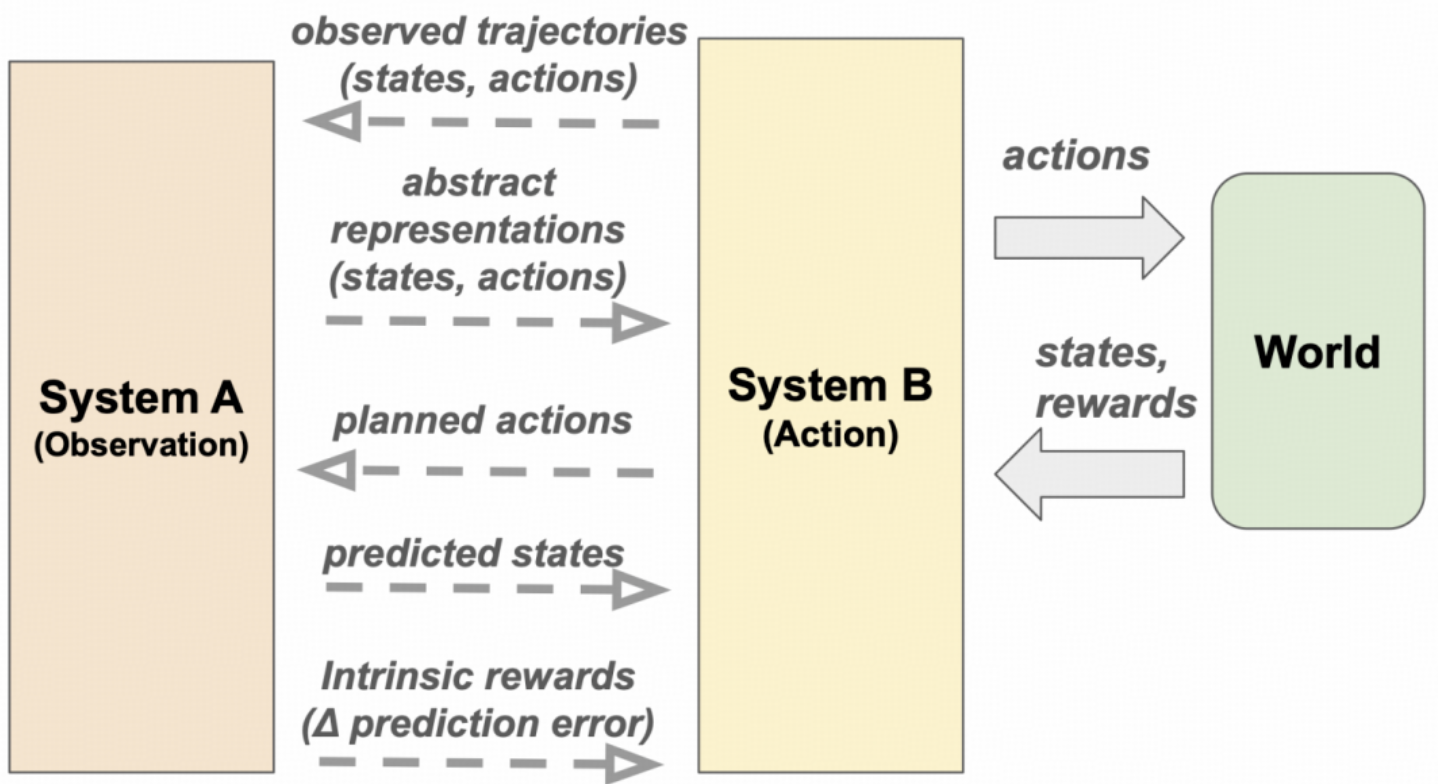
\includegraphics{images/image-0048.png}
\caption{A-B-M 自主学习架构示意图}
\end{figure}

\hypertarget{ux4e09ux53ccux5c42ux4f18ux5316}{%
\subsection{三、双层优化}\label{ux4e09ux53ccux5c42ux4f18ux5316}}

\textbf{内循环（发育尺度 Developmental Scale）}：这是单个智能体在其``一生''中的学习过程。利用给定的初始架构参数，系统 A 和系统 B 在固定的 System M 指挥下，与模拟环境实时交互、不断更新参数。

\textbf{外循环（演化尺度 Evolutionary Scale）}：在成千上万个模拟生命周期结束后，根据智能体是否完成了手工设计的生存适应度函数 \(\mathcal{L}\)，通过元学习算法去更新整个种群的``基因参数'' \(\phi\)。

数学形式化：

\[
\phi_{t+1} =
\arg\min_{\phi_t}
\mathcal{L}(A_0:A_K,B_0:B_K)
\]

这一优化必须受到开发育尺度的初始化和交互法则约束：

\[
A_0,B_0,M=\mathrm{Init}(\phi_t)
\]

\[
A_{i+1},B_{i+1}=\mathrm{Update}(M,A_i,B_i,Env)
\]

\hypertarget{ux56dbux9ad8ux7ea7ux5b66ux4e60ux5f62ux6001ux5c55ux671b}{%
\subsection{四、高级学习形态展望}\label{ux56dbux9ad8ux7ea7ux5b66ux4e60ux5f62ux6001ux5c55ux671b}}

在完善的元控制系统下，AI 有望展现出类似于大型哺乳动物和人类独有的高级学习形态：

\begin{itemize}
\tightlist
\item
  \textbf{通过沟通/社会化学习（Learning from Communication）}：System M 能够敏锐捕捉社会提示（如目光注视或教学语气），优先处理来自可靠来源（例如人类教师）的高优先级数据流，并快速同步给系统 A 建立新的世界规则。
\item
  \textbf{通过想象学习（Learning from Imagination）}：在休息甚至``睡眠''状态下，System M 能切断外部感官和运动输出，从情景记忆中提取经验进行高速回放，利用系统 A 在潜空间中推演长期计划，并在无需真实物理试错成本的情况下更新系统 B 的策略。
\end{itemize}

总结：这篇论文指出，想实现真正的通用人工智能并越过目前的数据墙，不应只依赖极度``语言中心化''且僵化的范式。AI 需要向认知科学取经，通过一个具有高度自决能力的元控制中心（System M），在``世界建模（观察）''和``具身控制（行动）''之间流畅切换，从而实现可以在部署后持续成长的自主生命体。

\hypertarget{ux53c2ux8003ux6587ux732e-153}{%
\subsection{参考文献}\label{ux53c2ux8003ux6587ux732e-153}}

\begin{itemize}
\tightlist
\item
  Dupoux, E., LeCun, Y., \& Malik, J. (2026). \href{https://arxiv.org/abs/2603.15381}{Why AI systems do not learn and what to do about it: Lessons on autonomous learning from cognitive science}. arXiv:2603.15381.
\end{itemize}

\clearpage


% 第5部分 世界模型、多模态生成与具身智能
\part*{第5部分 世界模型、多模态生成与具身智能}
\addcontentsline{toc}{part}{第5部分 世界模型、多模态生成与具身智能}


% 扩散模型与流匹配模型的原理和架构
\hypertarget{ux6269ux6563ux6a21ux578bux4e0eux6d41ux5339ux914dux6a21ux578bux7684ux539fux7406ux548cux67b6ux6784}{%
\chapter{扩散模型与流匹配模型的原理和架构}\label{ux6269ux6563ux6a21ux578bux4e0eux6d41ux5339ux914dux6a21ux578bux7684ux539fux7406ux548cux67b6ux6784}}

\hypertarget{ux6269ux6563ux6a21ux578bux7684ux57faux672cux539fux7406}{%
\section{扩散模型的基本原理}\label{ux6269ux6563ux6a21ux578bux7684ux57faux672cux539fux7406}}

\hypertarget{ux4e00ux524dux5411ux6269ux6563}{%
\subsection{一、前向扩散}\label{ux4e00ux524dux5411ux6269ux6563}}

给定从真实数据分布中采样的数据点，我们定义一个前向扩散过程，在该过程中，我们分步骤向样本添加少量高斯噪声，生成一系列含噪样本。步长由方差调度控制。随着步长的增大，数据样本逐渐失去其可区分的特征。最终，它等效于各向同性的高斯分布。

前向过程是一个固定的过程，它系统地、逐步地将一张清晰的原始图像 \(x_0\) 破坏成纯高斯噪声。

数学描述：该过程被定义为一个马尔可夫链，每一步只依赖于前一步。在每一步 \(t\)，我们向前一步的状态 \(x_{t-1}\) 添加高斯噪声得到：

\[
x_t = \sqrt{\alpha_t}\cdot x_{t-1} + \sqrt{1-\alpha_t}\cdot \epsilon_t
\]

其中，\(\epsilon_t \sim \mathcal{N}(0, I)\) 是标准高斯噪声，\(\alpha_t = 1-\beta_t\)，而 \(\beta_t\) 是一个预先设定的、随时间 \(t\) 增大而增大的噪声调度参数，控制着每一步添加的噪声量。

简单来说，使用 \(\sqrt{\alpha_t}\) 和 \(\sqrt{1-\alpha_t}\) 而不是直接使用 \(\alpha_t\) 和 \(1-\alpha_t\)，是为了保持数据的方差守恒，或者说防止数据在不断加噪的过程中``能量耗散''或``爆炸''。

根据期望的线性性质：

\[
\mathbb{E}[x_t]
= \mathbb{E}\left[\sqrt{\alpha_t}x_{t-1}+\sqrt{1-\alpha_t}\epsilon\right]
= \sqrt{\alpha_t}\mathbb{E}[x_{t-1}] + \sqrt{1-\alpha_t}\mathbb{E}[\epsilon]
= 0
\]

你会发现，无论系数用 \(\sqrt{\alpha}\) 还是 \(\alpha\)，甚至随便使用什么系数，只要输入和噪声的均值是 \(0\)，结果的均值永远是 \(0\)。所以，均值不是问题所在，它不需要我们操心。

\[
\begin{aligned}
x_t
&= \sqrt{\alpha_t}x_{t-1} + \sqrt{1-\alpha_t}\epsilon_{t-1},
\quad \text{where } \epsilon_{t-1},\epsilon_{t-2},\cdots \sim \mathcal{N}(0,I) \\
&= \sqrt{\alpha_t\alpha_{t-1}}x_{t-2}
 + \sqrt{1-\alpha_t\alpha_{t-1}}\bar{\epsilon}_{t-2},
\quad \text{where } \bar{\epsilon}_{t-2} \text{ merges two Gaussians } (*) \\
&= \cdots \\
&= \sqrt{\bar{\alpha}_t}x_0+\sqrt{1-\bar{\alpha}_t}\epsilon
\end{aligned}
\]

（*）表示涉及两个高斯分布的合并，数学推导此处暂略。

这里，\(\bar{\alpha}_t=\prod_{s=1}^{t}\alpha_s\) 是 \(\alpha_s\) 的累积乘积，\(\epsilon\sim\mathcal{N}(0,I)\)。这个公式极大地简化了过程，因为我们无需一步步迭代，就能直接获得任何中间噪声状态。当 \(t\) 足够大时（例如 \(T=1000\)），\(\bar{\alpha}_t\) 趋近于 \(0\)，\(x_T\) 就几乎变成了纯噪声 \(\epsilon\)。

前向扩散每一步递推的概率表示：

\[
q(x_t\mid x_{t-1}) = \mathcal{N}(x_t;\sqrt{1-\beta_t}x_{t-1},\beta_t I)
\]

等号右边表示用均值为 \(\sqrt{1-\beta_t}x_{t-1}\)、协方差为 \(\beta_t I\) 的高斯分布得到 \(x_t\)。

\hypertarget{ux4e8cux53cdux5411ux6269ux6563}{%
\subsection{二、反向扩散}\label{ux4e8cux53cdux5411ux6269ux6563}}

\begin{enumerate}
\def\labelenumi{\arabic{enumi}.}
\tightlist
\item
  数学推导
\end{enumerate}

在扩散模型的逆向过程（Reverse Process）中，我们的目标是从纯噪声 \(x_T\) 逐步还原出真实数据 \(x_0\)。理论上，从 \(x_t\) 倒推 \(x_{t-1}\) 的过程是一个条件概率分布 \(p_\theta(x_{t-1}\mid x_t)\)。

扩散模型的一个巧妙之处在于，当总步数 T足够大时，这个逆向条件概率可以近似为一个高斯分布：

\[
p(x_{t-1}\mid x_t)=\mathcal{N}(x_{t-1};\mu_\theta(x_t,t),\Sigma_\theta(x_t,t))
\]

这里有两个关键参数：均值 \(\mu_\theta\) 和方差 \(\Sigma_\theta\)。

\begin{itemize}
\tightlist
\item
  方差 \(\Sigma_\theta(x_t,t)\) 通常被设定为一个与时间步 \(t\) 相关的常数 \(\sigma_t^2 I\)，不需要网络学习。
\item
  因此，神经网络的根本任务是预测这个高斯分布的均值 \(\mu_\theta(x_t,t)\)。
\end{itemize}

也就是说说，扩散模型先预测一个确定性的噪声值，然后以此得到去噪后 \(x_{t-1}\) 的概率分布（高斯分布），从分布中抽样得到 \(x_{t-1}\)（随机性体现在这里）。下面求解该概率分布。

第一步：应用贝叶斯定理

我们的目标是求已知原始图像 \(x_0\) 时，真实的逆向转移概率 \(q(x_{t-1}\mid x_t,x_0)\)。直接求很困难，但利用贝叶斯定理，可以将其分解为几个已知的分布：

\[
q(x_{t-1}\mid x_t,x_0)
= \frac{q(x_t\mid x_{t-1},x_0)\cdot q(x_{t-1}\mid x_0)}{q(x_t\mid x_0)}
\]

根据扩散模型的马尔可夫性质，当前状态只依赖于前一个状态，因此 \(q(x_t\mid x_{t-1},x_0)=q(x_t\mid x_{t-1})\)。这个分布就是前向过程的定义：

\[
q(x_t\mid x_{t-1})=\mathcal{N}(x_t;\sqrt{\alpha_t}x_{t-1},(1-\alpha_t)I)
\]

而 \(q(x_{t-1}\mid x_0)\) 和 \(q(x_t\mid x_0)\) 是前向过程的闭式解，表示从 \(x_0\) 开始经过 \(t-1\) 步和 \(t\) 步加噪后的分布：

\begin{itemize}
\tightlist
\item
  \(q(x_t\mid x_{t-1})=\mathcal{N}(x_t\mid\sqrt{\alpha_t}x_{t-1},(1-\alpha_t)I)\)，表示从 \(x_{t-1}\) 到 \(x_t\) 的噪声添加。
\item
  \(q(x_{t-1}\mid x_0)=\mathcal{N}(x_{t-1}\mid\sqrt{\bar{\alpha}_{t-1}}x_0,(1-\bar{\alpha}_{t-1})I)\)，因为 \(x_{t-1}\) 是从 \(x_0\) 经过 \(t-1\) 步累积噪声得到的。
\item
  \(q(x_t\mid x_0)=\mathcal{N}(x_t\mid\sqrt{\bar{\alpha}_t}x_0,(1-\bar{\alpha}_t)I)\)，因为 \(x_t\) 是从 \(x_0\) 经过 \(t\) 步累积噪声得到的。
\end{itemize}

代入贝叶斯公式，得到：

\[
q(x_{t-1}\mid x_t,x_0)
= \frac{
\mathcal{N}(x_t\mid\sqrt{\alpha_t}x_{t-1},(1-\alpha_t)I)\cdot
\mathcal{N}(x_{t-1}\mid\sqrt{\bar{\alpha}_{t-1}}x_0,(1-\bar{\alpha}_{t-1})I)
}{
\mathcal{N}(x_t\mid\sqrt{\bar{\alpha}_t}x_0,(1-\bar{\alpha}_t)I)
}
\]

至此，我们将一个未知的分布分解成了三个已知的高斯分布。

第二步：合并高斯分布

我们希望证明这个分式的值也满足高斯分布，这里可以直接忽略归一化常数，只关注概率密度函数的指数部分，因为高斯分布的指数部分是二次型。从而：

\[
q(x_{t-1}\mid x_t,x_0)
\propto
\exp\left\{
-\frac{(x_t-\sqrt{\alpha_t}x_{t-1})^2}{2(1-\alpha_t)}
-\frac{(x_{t-1}-\sqrt{\bar{\alpha}_{t-1}}x_0)^2}{2(1-\bar{\alpha}_{t-1})}
+\frac{(x_t-\sqrt{\bar{\alpha}_t}x_0)^2}{2(1-\bar{\alpha}_t)}
\right\}
\]

定义二次函数：

\[
f(y)=
\frac{(x-\sqrt{a}y)^2}{2(1-a)}
+\frac{(y-\sqrt{b}z)^2}{2(1-b)}
-\frac{(x-\sqrt{c}z)^2}{2(1-c)}
\]

其中映射为：

\begin{itemize}
\tightlist
\item
  \(x=x_t\)，\(a=\alpha_t\)；
\item
  \(y=x_{t-1}\)，\(b=\bar{\alpha}_{t-1}\)，注意此处 \(b\) 使用累积参数 \(\bar{\alpha}_{t-1}\) 而非 \(\alpha_{t-1}\)；
\item
  \(z=x_0\)，\(c=\bar{\alpha}_t\)。
\end{itemize}

由于 \(f(y)\) 是二次函数，其最小值点即为高斯分布的均值。

对 \(f(y)\) 求导：

\[
f'(y)=-\frac{\sqrt{a}}{1-a}(x-\sqrt{a}y)+\frac{1}{1-b}(y-\sqrt{b}z)
\]

展开：

\[
f'(y)=\frac{a}{1-a}y-\frac{\sqrt{a}}{1-a}x+\frac{1}{1-b}y-\frac{\sqrt{b}}{1-b}z
\]

合并 \(y\) 项：

\[
f'(y)=\left(\frac{a}{1-a}+\frac{1}{1-b}\right)y-\frac{\sqrt{a}}{1-a}x-\frac{\sqrt{b}}{1-b}z
\]

令 \(f'(y)=0\)：

\[
y=\frac{\frac{\sqrt{a}}{1-a}x+\frac{\sqrt{b}}{1-b}z}{\frac{a}{1-a}+\frac{1}{1-b}}
\]

化简分母：

\[
\frac{a}{1-a}+\frac{1}{1-b}
=\frac{a(1-b)+(1-a)}{(1-a)(1-b)}
=\frac{1-ab}{(1-a)(1-b)}
\]

分子为：

\[
\frac{\sqrt{a}}{1-a}x+\frac{\sqrt{b}}{1-b}z
\]

因此：

\[
y=\frac{(1-b)\sqrt{a}x+(1-a)\sqrt{b}z}{1-ab}
\]

代入映射：

\begin{itemize}
\tightlist
\item
  \(a=\alpha_t\)；
\item
  \(b=\bar{\alpha}_{t-1}\)；
\item
  \(c=\bar{\alpha}_t\)；
\item
  \(ab=\alpha_t\cdot\bar{\alpha}_{t-1}=\bar{\alpha}_t\)，因为 \(\bar{\alpha}_t=\alpha_t\cdot\bar{\alpha}_{t-1}\)。
\end{itemize}

代入：

\[
y=\frac{(1-\bar{\alpha}_{t-1})\sqrt{\alpha_t}x_t+(1-\alpha_t)\sqrt{\bar{\alpha}_{t-1}}x_0}{1-\bar{\alpha}_t}
\]

这正是定理中给出的均值：

\[
\mu_q(x_t,x_0)=
\frac{(1-\bar{\alpha}_{t-1})\sqrt{\alpha_t}}{1-\bar{\alpha}_t}x_t
+\frac{(1-\alpha_t)\sqrt{\bar{\alpha}_{t-1}}}{1-\bar{\alpha}_t}x_0
\]

计算二阶导数：

\[
f''(y)=\frac{a}{1-a}+\frac{1}{1-b}
=\frac{a(1-b)+(1-a)}{(1-a)(1-b)}
=\frac{1-ab}{(1-a)(1-b)}
\]

代入：

\begin{itemize}
\tightlist
\item
  \(a=\alpha_t\)；
\item
  \(b=\bar{\alpha}_{t-1}\)；
\item
  \(ab=\bar{\alpha}_t\)。
\end{itemize}

于是：

\[
f''(y)=\frac{1-\bar{\alpha}_t}{(1-\alpha_t)(1-\bar{\alpha}_{t-1})}
\]

方差为倒数：

\[
\Sigma_q(t)=\frac{(1-\alpha_t)(1-\bar{\alpha}_{t-1})}{1-\bar{\alpha}_t}I
\]

从而最终结果为：

\[
\tilde{\mu}_t=
\frac{\sqrt{\alpha_t}(1-\bar{\alpha}_{t-1})}{1-\bar{\alpha}_t}x_t
+\frac{\sqrt{\bar{\alpha}_{t-1}}(1-\alpha_t)}{1-\bar{\alpha}_t}x_0
\]

\[
\tilde{\beta}_t=\frac{(1-\alpha_t)(1-\bar{\alpha}_{t-1})}{1-\bar{\alpha}_t}
\]

这个公式表明，在已知原始图像 \(x_0\) 的条件下，逆向分布的均值是当前噪声图像 \(x_t\) 和原始图像 \(x_0\) 的线性组合。

第三步：参数化重写表达式

上面的均值公式仍然依赖于我们不知道的 \(x_0\)。这时，前向过程的重参数化技巧发挥了关键作用。前向过程告诉我们，任意时刻的 \(x_t\) 可以直接由 \(x_0\) 和一个小噪声 \(\epsilon\) 表示：

\[
x_t=\sqrt{\bar{\alpha}_t}x_0+\sqrt{1-\bar{\alpha}_t}\epsilon,\quad \epsilon\sim\mathcal{N}(0,I)
\]

我们可以从这个等式中解出 \(x_0\)：

\[
x_0=\frac{x_t-\sqrt{1-\bar{\alpha}_t}\epsilon}{\sqrt{\bar{\alpha}_t}}
\]

现在，将 \(x_0\) 的表达式代入第二步得到的均值公式中：

\[
\tilde{\mu}_t=
\frac{\sqrt{\alpha_t}(1-\bar{\alpha}_{t-1})}{1-\bar{\alpha}_t}x_t
+\frac{\sqrt{\bar{\alpha}_{t-1}}(1-\alpha_t)}{1-\bar{\alpha}_t}
\left(\frac{x_t-\sqrt{1-\bar{\alpha}_t}\epsilon}{\sqrt{\bar{\alpha}_t}}\right)
\]

接下来的工作就是合并同类项进行化简。经过一些代数运算，可以得到一个极其简洁的形式：

\[
\tilde{\mu}_t=\frac{1}{\sqrt{\alpha_t}}
\left(x_t-\frac{1-\alpha_t}{\sqrt{1-\bar{\alpha}_t}}\epsilon\right)
\]

这里的 \(\epsilon\) 表示从 \(x_0\) 到 \(x_t\) 的步骤加入的``总等价噪声''。
而真实数据是已被确定的情况下，这一步预测的方差仍由 \(\alpha_t=1-\beta_t\) 决定：

\[
\tilde{\mu}_t=
\frac{\sqrt{\alpha_t}(1-\bar{\alpha}_{t-1})}{1-\bar{\alpha}_t}x_t
+\frac{\sqrt{\bar{\alpha}_{t-1}}(1-\alpha_t)}{1-\bar{\alpha}_t}x_0
\]

\[
\tilde{\beta}_t=\frac{(1-\alpha_t)(1-\bar{\alpha}_{t-1})}{1-\bar{\alpha}_t}
\]

这个公式表明，在已知原始图像 \(x_0\) 的条件下，逆向分布的均值是当前噪声图像 \(x_t\) 和原始图像 \(x_0\) 的线性组合。
关于方差的更多讨论见Diffusion Transformer部分。

\begin{enumerate}
\def\labelenumi{\arabic{enumi}.}
\setcounter{enumi}{1}
\tightlist
\item
  在模型中的应用
\end{enumerate}

以上公式让我们，如果我们能知道在前向过程中第 \(t\) 步所添加的噪声 \(\epsilon_t\)，那么我们就可以精确地计算出逆向步骤的均值，从而从 \(x_t\) 回归到 \(x_{t-1}\) 的分布。但问题在于，我们只知道噪声满足高斯分布 \(\mathcal{N}(0,I)\)，但对于在这个分布中具体采样了什么值，以使得原始的 \(x_0\) 变为充满噪声的 \(x_t\) 一无所知。

既然我们无法预先知道 \(\epsilon\)，那么就训练一个神经网络 \(\epsilon_\theta\) 来学习预测这个噪声。训练目标就是最小化预测噪声 \(\epsilon_\theta(x_t,t)\) 和真实噪声 \(\epsilon\) 之间的均方损失（差距）。这将复杂的分布预测问题转化为更稳定的噪声预测问题，大大降低了模型的学习难度。

这种设置与变分自编码器（VAE）非常相似，因此我们可以使用变分下界来优化负对数似然。

\hypertarget{ux4e09ux6269ux6563ux6a21ux578bux7684ux8badux7ec3}{%
\subsection{三、扩散模型的训练}\label{ux4e09ux6269ux6563ux6a21ux578bux7684ux8badux7ec3}}

\begin{enumerate}
\def\labelenumi{\arabic{enumi}.}
\tightlist
\item
  训练时去噪起点的步数随机采样
\end{enumerate}

在扩散模型的理论框架中，生成过程（反向去噪）是一个马尔可夫链（Markov Chain），需要从 \(t=T\) 一步步倒退回 \(t=0\)。

如果我们在训练时也按照 \(T,T-1,\ldots,0\) 的顺序串行训练，会导致两个致命问题：

\begin{enumerate}
\def\labelenumi{\arabic{enumi}.}
\tightlist
\item
  \textbf{计算成本极高}：每次反向传播都要穿越整个时间链，由于梯度累积，显存会直接撑爆。
\item
  \textbf{误差级联}：前面的步骤如果没学好，后面的步骤就会在错误的输入上越走越偏。
\end{enumerate}

为了解决这个问题，DDPM（Denoising Diffusion Probabilistic Models）的作者利用了高斯分布的``可加性''（重参数化技巧），推导出了一个惊艳的结论：\textbf{我们不需要一步步加噪，而是可以直接写出任意时刻 \(t\) 的状态解析解}。

\[
x_t=\sqrt{\bar{\alpha}_t}x_0+\sqrt{1-\bar{\alpha}_t}\epsilon
\]

有了这个公式，模型的最终优化目标（变分下界 ELBO 的简化版）可以写成对所有时间步 \(t\) 的期望：

\[
\mathcal{L}_{simple}
=\mathbb{E}_{t\sim\mathcal{U}(1,T),\,x_0\sim q(x_0),\,\epsilon\sim\mathcal{N}(0,I)}
\left[\left\|\epsilon-\epsilon_\theta(x_t,t)\right\|^2\right]
\]

数学上的核心就在这里：公式外层的 \(\mathbb{E}_{t\sim\mathcal{U}(1,T)}\) 表示损失函数是对均匀分布的 \(t\) 求期望。在实际写代码训练时，计算这个全局期望的方法就是蒙特卡洛采样（Monte Carlo Sampling），即在每个 Batch 中，随机均匀地抽取 \(t\)。

\begin{enumerate}
\def\labelenumi{\arabic{enumi}.}
\setcounter{enumi}{1}
\tightlist
\item
  并行性
\end{enumerate}

扩散模型的每一步都是同时对所有 token 去噪，因而处理过程是并行的。从概率论的角度：

假设我们要生成一个句子：

\[
X = \{x_1, x_2, x_3, x_4\}
\]

自回归模型模型严格遵循概率的链式法则：

\[
P(X) = P(x_1)P(x_2 \mid x_1)P(x_3 \mid x_1, x_2)P(x_4 \mid x_1, x_2, x_3)
\]

要算 \(x_3\)，必须先有确定的 \(x_1,x_2\)。

而扩散模型的目标是直接模拟联合分布 \(P(x_1,x_2,x_3,x_4)\)。在生成的某一步骤中（例如从 \(X^{(T+1)}\) 去噪到 \(X^{(T)}\)），模型通常假设：各个位置的预测在当前步骤是条件独立的，也就是 \(x_1^{(T)},x_2^{(T)},\ldots,x_N^{(T)}\) 相互独立。我们只通过上一步的全局上下文 \(x_1^{(T+1)},x_2^{(T+1)},\ldots,x_N^{(T+1)}\) 来推断本步的 \(x_i^{(T)}\)，即根据``全局的模糊轮廓''来同时填补所有细节。这样，在文本扩散中，公式往往近似为：

\[
\begin{aligned}
P(X^{(T)} \mid X^{(T+1)})
&\approx
P(x_1^{(T)} \mid x_1^{(T+1)},x_2^{(T+1)},\ldots) \\
&\quad \cdot P(x_2^{(T)} \mid x_1^{(T+1)},x_2^{(T+1)},\ldots) \\
&\quad \cdots
P(x_N^{(T)} \mid x_1^{(T+1)},x_2^{(T+1)},\ldots)
\end{aligned}
\]

这样，在一步预测中，猜测 \(x_2\) 就不需要等待 \(x_1\) 先去噪，能提高 GPU 的利用效率。

在文本生成等任务中，扩散模型的生成质量不如自回归模型。虽然扩散模型可以通过并行一次生成10个词，但由于它在单步生成时，假设了这些词是并行独立生成的（或者仅依赖于上一轮的模糊状态），它往往忽略了词与词之间微小的因果强关联。自回归的做法： ``因为第一个词是`人工'，所以第二个词大概率是`智能'。''（强因果）纯并行的做法： ``我看整体语境像是一个科技话题，所以位置1我猜`人工'，位置2我猜`智能'。''如果并行度太高，有时候会出现逻辑不自洽，在更复杂的推理任务中容易导致逻辑断裂。

\begin{enumerate}
\def\labelenumi{\arabic{enumi}.}
\setcounter{enumi}{2}
\tightlist
\item
  训练算法工作流
\end{enumerate}

通过随机抽取 \(t\)，扩散模型极其优雅地将一个串行的时序生成问题，拆解成了完全可以并行训练的独立去噪任务。具体的算法工作流如下：

\begin{itemize}
\tightlist
\item
  \textbf{Step 1: 采样真实数据。} 从训练集中随机抽取一张干净的真实图像 \(x_0\sim q(x_0)\)。
\item
  \textbf{Step 2: 随机采样时间步。} 从均匀分布中随机抽取一个时间步 \(t\sim\mathcal{U}(1,T)\)（通常 \(T=1000\)）。
\item
  \textbf{Step 3: 采样标准高斯噪声。} 生成一个与 \(x_0\) 维度完全相同的随机噪声矩阵 \(\epsilon\sim\mathcal{N}(0,I)\)。
\item
  \textbf{Step 4: 一步到位构建加噪图像。} 利用刚才推导出的闭式解公式 \(x_t=\sqrt{\bar{\alpha}_t}x_0+\sqrt{1-\bar{\alpha}_t}\epsilon\)，直接计算出图像在时刻 \(t\) 的加噪状态 \(x_t\)。
\item
  \textbf{Step 5: 神经网络预测。} 将加噪图像 \(x_t\) 和时间步 \(t\)（通常经过正弦位置编码）一起输入到神经网络 \(\epsilon_\theta\)（如 U-Net 或 DiT）中，让网络预测出刚才添加的噪声 \(\epsilon_\theta(x_t,t)\)。
\item
  \textbf{Step 6: 计算损失并更新梯度。} 计算真实噪声 \(\epsilon\) 和预测噪声 \(\epsilon_\theta\) 之间的均方误差（MSE），进行反向传播更新网络权重。
\end{itemize}

\hypertarget{ux53c2ux8003ux6587ux732e-154}{%
\subsection{参考文献}\label{ux53c2ux8003ux6587ux732e-154}}

\begin{itemize}
\tightlist
\item
  Ho, J., Jain, A., \& Abbeel, P. (2020). \href{https://arxiv.org/abs/2006.11239}{Denoising Diffusion Probabilistic Models}. NeurIPS.
\item
  Song, Y., Sohl-Dickstein, J., Kingma, D. P., Kumar, A., Ermon, S., \& Poole, B. (2021). \href{https://arxiv.org/abs/2011.13456}{Score-Based Generative Modeling through Stochastic Differential Equations}. ICLR.
\item
  Song, J., Meng, C., \& Ermon, S. (2021). \href{https://arxiv.org/abs/2010.02502}{Denoising Diffusion Implicit Models}. ICLR.
\end{itemize}

\clearpage

\hypertarget{ux968fux673aux68afux5ea6ux6717ux4e4bux4e07ux52a8ux529bux5b66}{%
\section{随机梯度朗之万动力学}\label{ux968fux673aux68afux5ea6ux6717ux4e4bux4e07ux52a8ux529bux5b66}}

\hypertarget{ux4e00ux968fux673aux68afux5ea6ux6717ux4e4bux4e07ux52a8ux529bux5b66ux7684ux6570ux5b66ux8868ux8fbe}{%
\subsection{一、随机梯度朗之万动力学的数学表达}\label{ux4e00ux968fux673aux68afux5ea6ux6717ux4e4bux4e07ux52a8ux529bux5b66ux7684ux6570ux5b66ux8868ux8fbe}}

朗之万动力学最初源于物理学，用于描述粒子在势能场中的随机运动。在机器学习中，随机梯度朗之万动力学（Stochastic Gradient Langevin Dynamics, SGLD）将参数优化视为一个``粒子''在能量景观（由损失函数定义）中的运动过程。其离散化的更新公式为：

假设我们想要从一个未知的目标真实数据分布 \(p(x)\) 中采样出一张图像 \(x\)。朗之万动力学提供了一个迭代公式：

\[
x_{i+1}=x_i+\frac{\gamma}{2}\nabla_x\log p(x_i)+\sqrt{\gamma}z_i
\]

其中：

\begin{itemize}
\tightlist
\item
  \(x_i\) 是第 \(i\) 步的状态（图像向量）。
\item
  \(\gamma\) 是步长（Step size）。
\item
  \(z_i\sim\mathcal{N}(0,I)\) 是标准高斯噪声。
\item
  \(\nabla_x\log p(x_i)\) 被称为得分函数（Score Function），它是目标分布的对数概率密度函数对输入 \(x\) 的梯度。
\end{itemize}

这个公式包含两部分力量的博弈：

\begin{enumerate}
\def\labelenumi{\arabic{enumi}.}
\tightlist
\item
  \textbf{确定性漂移（梯度上升）}：\(\frac{\gamma}{2}\nabla_x\log p(x_i)\) 牵引着数据点 \(x_i\) 沿着概率密度增加最快的方向（爬山）移动，让图像越来越像真实图像。
\item
  \textbf{随机性扩散（噪声注入）}：\(\sqrt{\gamma}z_i\) 不断注入随机的扰动。这不仅是为了防止模型陷入局部最优（例如前文提到的``撞树''的均值点），更是为了确保最终的样本在整个高维空间中能够严格服从真实的 \(p(x)\) 分布，而不是仅仅坍缩到一个单一的最高概率点。
\end{enumerate}

看似只是加了噪声，实际上反映出它和常规的梯度下降目标不同：

梯度下降是一种优化算法，其目标是找到损失函数的（局部或全局）最小值点，得到一个点估计（Point Estimate），对应的是最大后验概率（MAP）估计。

SGLD是一种贝叶斯采样算法，其目标不是找到一个``最佳''点，而是通过采样来近似整个后验分布。这允许我们进行不确定性量化，即了解参数估计的可靠程度。

为什么这样采样能近似后验分布：

\[
\Delta\theta_t=-\frac{\epsilon_t}{2}\nabla\tilde{U}(\theta_t)+\sqrt{\epsilon_t}\cdot\eta_t,\quad \eta_t\sim\mathcal{N}(0,I)
\]

这个公式包含两部分：

\begin{enumerate}
\def\labelenumi{\arabic{enumi}.}
\tightlist
\item
  \(-\frac{\epsilon_t}{2}\nabla\tilde{U}(\theta_t)\)：这是随机梯度下降部分。它试图将参数推向后验概率最大的地方（MAP 估计）。
\item
  \(\sqrt{\epsilon_t}\cdot\eta_t\)：这是注入的高斯噪声部分。
\end{enumerate}

关键的 \(\sqrt{\epsilon}\) Scaling：

请注意，梯度的系数是 \(\epsilon\)（步长），而噪声的系数是 \(\sqrt{\epsilon}\)。当步长 \(\epsilon\to 0\) 时，噪声项 \(\sqrt{\epsilon}\) 会比梯度项 \(\epsilon\) 大得多（因为 \(0.0001\ll\sqrt{0.0001}=0.01\)）。

这保证了即使到了谷底（梯度接近 0），噪声依然主导，迫使参数继续跳动。

根据 Fokker-Planck 方程的推导，上述随机过程的稳态分布（Stationary Distribution）精确地收敛于：

\[
p(\theta)\propto \exp(-U(\theta))
\]

也就是我们的后验分布。
另外，当面对大规模数据集时，计算完整数据集的真实梯度 \(\nabla_x L(x_t)\) 计算成本极高。SGLD 使用基于一个小批量（mini-batch）数据 \(\xi_t\) 计算的随机梯度 \(\nabla_x L(x_t;\xi_t)\) 来近似代替真实梯度，进行上述计算。最终生成的参数序列 \(\{x_t\}\) 也会收敛到真实的后验分布 \(p(x\mid\mathrm{data})\)。

\hypertarget{ux4e8cux5f97ux5206ux5339ux914d}{%
\subsection{二、得分匹配}\label{ux4e8cux5f97ux5206ux5339ux914d}}

要运行朗之万动力学，我们必须知道 \(\nabla_x\log p(x)\)。但在现实中，\(p(x)\) 是极其复杂的。通常概率分布可以写成基于能量的形式：

\[
p(x)=\frac{e^{-E_\theta(x)}}{Z_\theta}
\]

这里 \(Z_\theta=\int e^{-E_\theta(x)}dx\) 是配分函数。在高维像素空间中，对所有可能的图像求和或积分计算 \(Z_\theta\) 是绝对不可能的（Intractable）。

\textbf{得分函数的神奇之处在于它消除了 \(Z_\theta\)：}

\[
\nabla_x\log p(x)=\nabla_x(-E_\theta(x)-\log Z_\theta)=-\nabla_x E_\theta(x)
\]

因为 \(Z_\theta\) 是一个常数，对 \(x\) 求导直接等于 0。因此，我们可以直接训练一个神经网络 \(s_\theta(x)\) 去拟合这个得分：

\[
s_\theta(x)\approx\nabla_x\log p(x)
\]

这个过程被称为得分匹配（Score Matching）。

\hypertarget{ux4e09ux6269ux6563ux6a21ux578bux7684ux672cux8d28}{%
\subsection{三、扩散模型的本质}\label{ux4e09ux6269ux6563ux6a21ux578bux7684ux672cux8d28}}

在 DDPM 中，神经网络 \(\epsilon_\theta(x_t,t)\) 预测的是噪声 \(\epsilon\)。在数学上，预测噪声与预测得分是完全等价的。它们之间的转换公式为：

\[
\nabla_{x_t}\log p(x_t)=-\frac{\epsilon_\theta(x_t,t)}{\sqrt{1-\bar{\alpha}_t}}
\]

因此，DDPM 中的去噪网络本质上就是一个得分估计器。当 DDPM 使用 Euler-Maruyama 方法求解反向 SDE 时，它所执行的每一步去噪操作，本质上就是带有特定系数的退火朗之万动力学（Annealed Langevin Dynamics）。

DDPM 原始的反向采样公式（从 \(x_t\) 生成 \(x_{t-1}\)）长这样：

\[
x_{t-1}=\frac{1}{\sqrt{\alpha_t}}
\left(x_t-\frac{1-\alpha_t}{\sqrt{1-\bar{\alpha}_t}}\epsilon_\theta(x_t,t)\right)
+\sigma_t z
\]

现在，我们将上面的``翻译桥梁''代入这个公式，把 \(\epsilon_\theta\) 替换成梯度的形式，公式就变成了基于得分的形式：

\[
x_{t-1}=\frac{1}{\sqrt{\alpha_t}}x_t
+\frac{1-\alpha_t}{\sqrt{\alpha_t}}\nabla_{x_t}\log p_t(x_t)
+\sigma_t z
\]

为了对比，我们把标准的朗之万动力学迭代公式也写在下面：

\[
x_{i+1}=x_i+\frac{\gamma}{2}\nabla_x\log p(x_i)+\sqrt{\gamma}\epsilon
\]

现在，这两者的逐项对应关系就变得极其清晰了：

\begin{enumerate}
\def\labelenumi{\arabic{enumi}.}
\tightlist
\item
  \textbf{梯度引导项（确定性漂移）}
\end{enumerate}

朗之万动力学：\(\frac{\gamma}{2}\nabla_x\log p(x_i)\)。代表沿着概率密度的梯度方向（即数据流形的方向）爬升，步长为 \(\frac{\gamma}{2}\)。

扩散模型：\(\frac{1-\alpha_t}{\sqrt{\alpha_t}}\nabla_{x_t}\log p_t(x_t)\)。这正是 DDPM 在每一步去噪时，利用神经网络推动图像走向真实分布的力量。在这里，\(\frac{1-\alpha_t}{\sqrt{\alpha_t}}\) 精确等价于朗之万动力学中的步长系数 \(\frac{\gamma}{2}\)。随着 \(t\) 减小，这个步长也会动态衰减（退火）。

\begin{enumerate}
\def\labelenumi{\arabic{enumi}.}
\setcounter{enumi}{1}
\tightlist
\item
  \textbf{噪声注入项（随机游走）}
\end{enumerate}

朗之万动力学：\(\sqrt{\gamma}\epsilon\)。为了防止陷入局部最优和维持分布特性的随机扰动。

扩散模型：\(\sigma_t z\)。其中 \(z\sim\mathcal{N}(0,I)\)。在 DDPM 中，方差 \(\sigma_t^2\) 通常被设定为 \(\beta_t\) 或 \(\tilde{\beta}_t\)。这完美对应了朗之万采样的随机注入部分。它在具身智能中打破``多模态均值（撞树）''僵局的物理力量，就来源于这一项。

\begin{enumerate}
\def\labelenumi{\arabic{enumi}.}
\setcounter{enumi}{2}
\tightlist
\item
  \textbf{状态缩放项（阻尼/动量）}
\end{enumerate}

朗之万动力学：\(x_i\)（前面系数为 1）。

扩散模型：\(\frac{1}{\sqrt{\alpha_t}}x_t\)。

\textbf{为什么有差异？} 这是因为 DDPM 的前向加噪过程不仅仅是简单地加噪声，它是一个奥恩斯坦-乌伦贝克过程（Ornstein-Uhlenbeck Process, OU 过程）。在前向时，为了防止图像像素的方差随时间爆炸，DDPM 每一步都会将图像按比例缩小（乘以 \(\sqrt{\alpha_t}\)）。因此，在反向 Langevin 采样时，必须除以 \(\sqrt{\alpha_t}\) 来补偿之前的缩放。这相当于物理学中带有``阻尼''或``向心力''的朗之万动力学。

\hypertarget{ux56dbux5faeux5206ux65b9ux7a0bux8868ux793a}{%
\subsection{四、微分方程表示}\label{ux56dbux5faeux5206ux65b9ux7a0bux8868ux793a}}

传统的 DDPM（如 Ho 等人提出的形式）是离散步长的。当我们将加噪和去噪的步数 \(T\to\infty\) 时，离散的马尔可夫链就变成了一个连续时间的随机微分方程（SDE）。

\begin{enumerate}
\def\labelenumi{\arabic{enumi}.}
\tightlist
\item
  \textbf{前向加噪过程（破坏数据）}
\end{enumerate}

前向过程可以通过如下的 SDE 描述：

\[
dx=f(x,t)dt+g(t)dw
\]

其中 \(w\) 是标准的布朗运动（连续时间的随机游走），\(f(x,t)\) 是漂移系数，\(g(t)\) 是扩散系数。这个过程不需要任何网络参与，纯粹是通过物理规则把清晰图像 \(x_0\) 变成纯噪声 \(x_T\)。

\begin{enumerate}
\def\labelenumi{\arabic{enumi}.}
\setcounter{enumi}{1}
\tightlist
\item
  \textbf{反向生成过程（朗之万动力学的连续体现）}
\end{enumerate}

根据 Anderson 定理，任何形式如上的前向 SDE，都存在一个对应的反向 SDE，用于从噪声 \(x_T\) 逆向生成真实数据 \(x_0\)：

\[
dx=\left[f(x,t)-g(t)^2\nabla_x\log p_t(x)\right]dt+g(t)d\bar{w}
\]

这里的 \(d\bar{w}\) 是时间反转下的布朗运动。观察这个反向 SDE 的核心项：\(-g(t)^2\nabla_x\log p_t(x)\)。它精确地对应了朗之万动力学中的梯度引导项。

\hypertarget{ux53c2ux8003ux6587ux732e-155}{%
\subsection{参考文献}\label{ux53c2ux8003ux6587ux732e-155}}

\begin{itemize}
\tightlist
\item
  Welling, M., \& Teh, Y. W. (2011). \href{https://www.stats.ox.ac.uk/~teh/research/compstats/WelTeh2011a.pdf}{Bayesian Learning via Stochastic Gradient Langevin Dynamics}. ICML.
\item
  Roberts, G. O., \& Tweedie, R. L. (1996). \href{https://doi.org/10.2307/3318418}{Exponential Convergence of Langevin Distributions and Their Discrete Approximations}. Bernoulli.
\end{itemize}

\clearpage

\hypertarget{diffusion-u-net}{%
\section{Diffusion U-Net}\label{diffusion-u-net}}

U-Net采用卷积神经网络，前半部分类似Encoder，通过池化或步长＞1的卷积，使空间尺寸数不断减小、通道数不断增大；后半部分类似Decoder，空间尺寸数不断增大、通道数不断减小，主要有两种实现方法：

\textbf{1. 转置卷积（Transposed Convolution）}

这是 U-Net 解码器中使用的核心放大技术。它不仅仅是简单的图像插值，而是一个带有可学习参数的逆向空间扩散过程。

在标准卷积中，我们可以将其表示为矩阵乘法 \(\mathbf{Y}=\mathbf{C}\mathbf{X}\)，其中 \(\mathbf{C}\) 是由卷积核转换而来的稀疏矩阵，此过程将大维度的 \(\mathbf{X}\) 压缩为小维度的 \(\mathbf{Y}\)。

转置卷积则是将输出特征图通过乘以 \(\mathbf{C}\) 的转置矩阵 \(\mathbf{C}^T\)（并通过反向传播学习权重）还原到更大的空间：

\[
\mathbf{X}'=\mathbf{C}^T\mathbf{Y}
\]

工作流：

以卷积核大小 \(K=3\)、步长 \(S=2\)、填充 \(P=1\) 为例：

\begin{enumerate}
\def\labelenumi{\arabic{enumi}.}
\tightlist
\item
  \textbf{内部零填充（Zero-padding expansion）}：在输入特征图的相邻像素之间插入 \(S-1\) 个零。这会将低分辨率输入的空间尺寸强行撑大。
\item
  \textbf{边界填充}：在扩展后的特征图四周边缘添加额外的零填充（数量由 \(K\) 和 \(P\) 决定，以精确对齐所需输出的尺寸）。
\item
  \textbf{标准卷积映射}：对上述经过两次填充的巨大特征图，应用一个标准的 \(K\times K\) 卷积核（此时卷积的步长固定为 1）。
\item
  \textbf{特征输出}：卷积核在滑动计算过程中，将原始孤立像素的值与其权重相乘并``扩散''到周围插零的区域，最终输出平滑的高分辨率特征图。
\end{enumerate}

\textbf{2. 双线性插值（Bilinear Interpolation）}

这是一种无参数的纯数学插值方法。它通过计算目标像素在原图中对应位置周围四个已知像素的加权平均值来生成新像素。它的计算成本极低，但无法像转置卷积那样根据数据集的特征自适应学习放大规则。

但U-Net的可扩展性一般，且与当前基于Transformer的大模型架构不兼容。

\hypertarget{ux53c2ux8003ux6587ux732e-156}{%
\subsection{参考文献}\label{ux53c2ux8003ux6587ux732e-156}}

\begin{itemize}
\tightlist
\item
  Ronneberger, O., Fischer, P., \& Brox, T. (2015). \href{https://arxiv.org/abs/1505.04597}{U-Net: Convolutional Networks for Biomedical Image Segmentation}. MICCAI.
\item
  Ho, J., Jain, A., \& Abbeel, P. (2020). \href{https://arxiv.org/abs/2006.11239}{Denoising Diffusion Probabilistic Models}. NeurIPS.
\item
  Rombach, R., Blattmann, A., Lorenz, D., Esser, P., \& Ommer, B. (2022). \href{https://arxiv.org/abs/2112.10752}{High-Resolution Image Synthesis with Latent Diffusion Models}. CVPR.
\end{itemize}

\clearpage

\hypertarget{diffusion-transformer}{%
\section{Diffusion Transformer}\label{diffusion-transformer}}

\hypertarget{ux4e00ux6838ux5fc3ux67b6ux6784ux4e0eux5de5ux4f5cux6d41}{%
\subsection{一、核心架构与工作流}\label{ux4e00ux6838ux5fc3ux67b6ux6784ux4e0eux5de5ux4f5cux6d41}}

Diffusion Transformer将Transformer架构引入扩散模型，实现了与大语言模型架构的统一，也提高了可扩展性，使得生成质量可随着模型参数的扩大而提升。

\begin{enumerate}
\def\labelenumi{\arabic{enumi}.}
\tightlist
\item
  \textbf{潜在空间分块（Latent Patchification）}
\end{enumerate}

DiT 并不直接操作像素，而是操作 VAE（变分自编码器）编码后的潜在特征。

给定一张输入图像 \(x\in\mathbb{R}^{H\times W\times 3}\)，首先通过预训练的 VAE 编码器将其映射到潜在空间，得到潜在表示 \(z\in\mathbb{R}^{h\times w\times c}\)。

接着，DiT 将 \(z\) 切分为大小为 \(p\times p\) 的空间块（Patches），将这些块展平并经过线性投影，转换为序列长度为 \(T=(h/p)\times(w/p)\)、维度为 \(d\) 的 Token 序列。最后，加上标准的可学习位置编码（Positional Embeddings）。

\begin{enumerate}
\def\labelenumi{\arabic{enumi}.}
\setcounter{enumi}{1}
\tightlist
\item
  \textbf{条件注入机制：adaLN-Zero Block}
\end{enumerate}

标准的扩散模型需要在每个去噪步骤中注入当前的时间步 \(t\) 和条件类别 \(c\)。U-Net 通常通过交叉注意力（Cross-Attention）或特征拼接来实现，而 DiT 采用了自适应层归一化（Adaptive Layer Normalization, adaLN）。

这是 DiT 架构中最关键的设计。对于传入 DiT Block 的隐藏层状态 \(h\)，adaLN 的操作如下：

\[
\mathrm{adaLN}(h,t,c)=\gamma_{(t,c)}\mathrm{LayerNorm}(h)+\beta_{(t,c)}
\]

其中，缩放参数 \(\gamma_{(t,c)}\) 和平移参数 \(\beta_{(t,c)}\) 是通过对时间步嵌入和类别嵌入的加和应用一个多层感知机（MLP）回归直接生成的，而不是作为可学习参数固定在网络中。

此外，DiT 还引入了\textbf{门控机制（Dimension Scaling）}，用于残差连接之前。为了极大地稳定训练，作者提出了 \textbf{adaLN-Zero} 初始化策略：即强制 MLP 在初始化时输出的 \(\gamma_{(t,c)}\)、\(\beta_{(t,c)}\) 以及残差门控参数 \(\alpha_{(t,c)}\) 全部为零。

这意味着在训练初始阶段，\textbf{每一个 DiT Block 都是一个严格的恒等映射（Identity Function）}：

\[
h_{l+1}=h_l+0=h_l
\]

这保证了网络在初始状态下不会因为深层 Transformer 的高方差而崩溃。

\begin{enumerate}
\def\labelenumi{\arabic{enumi}.}
\setcounter{enumi}{2}
\tightlist
\item
  \textbf{Unpatchification（去块化与预测）}
\end{enumerate}

在经过 \(N\) 层 DiT Block 后，Token 序列被送入最后一个标准的全连接层，将维度扩张回 \(p\times p\times 2c\)（乘以 2 是因为模型需要同时预测噪声和方差）。随后，将一维序列重新排列（Reshape）回 \(h\times w\times 2c\) 的空间网格结构，输出给后续的损失函数计算或采样。
我们发现adaLN只能注入定长向量 \(c\)，如 \texttt{{[}CLS{]}} token。但显然一个 token 不够，故可以引入基于多模态双流注意力的MM-DiT：（扩散和自回归结合的模型，自回归上下文越来越长，也是运用了此方法）

先对图像流和文本流各自AdaLN（自适应层归一化）后各自计算Q、K、V，然后将图像的QKV和文本的QKV直接拼接（Concatenate）在一起，在这个拼接好的超长序列上，执行一次全局的自注意力机制，图像、文本可以内部信息融合，也可以让图像提取对应文本提示、文本根据图像更新上下文。

注意力计算完成后，将输出的超长序列重新切开，恢复成图像特征和文本特征。然后分别送入各自的残差连接和前馈神经网络（FFN），并应用AdaLN预测的门控系数。

（此处图片与上文 adaLN-Zero 初始化和 Unpatchification 说明重复，已合并转写。）

\begin{enumerate}
\def\labelenumi{\arabic{enumi}.}
\setcounter{enumi}{3}
\tightlist
\item
  注意力模块和自回归Transformer的不同点
\end{enumerate}

对于扩散模型，在任何一个注意力层，所有的 token 必须同时相互计算注意力，最终也会同时输出所有 token 对应的向量。这就要求在显存中实打实地实例化一个 \(N\times N\) 的注意力分数矩阵。而且如果扩散 \(K\) 步，就要对这个矩阵计算 \(K\) 次。对于视频生成模型，\(N=\mathcjk{帧数}\times\mathcjk{patch\mathcjk{数}}\)，这也就是为什么很多视频生成模型采用``块内扩散、块间自回归''的方式。

\textbf{训练阶段工作流}

\begin{enumerate}
\def\labelenumi{\arabic{enumi}.}
\tightlist
\item
  \textbf{图像编码}：将原始图像 \(x\) 输入冻结权重的 VAE 编码器，提取潜在特征 \(z_0\)。
\item
  \textbf{随机加噪}：随机采样一个时间步 \(t\sim U(1,T)\) 和标准高斯噪声 \(\epsilon\sim\mathcal{N}(0,I)\)。根据前向公式计算得到加噪后的潜在变量 \(z_t\)。
\item
  \textbf{块化处理（Patchify）}：将 \(z_t\) 切分为多个 Patch，展平并加上位置编码，形成输入序列。
\item
  \textbf{条件嵌入}：将时间步 \(t\) 和图像对应的类别标签 \(c\) 转化为条件向量（通过 Embedding 层和 MLP）。
\item
  \textbf{DiT 前向传播}：

  \begin{itemize}
  \tightlist
  \item
    将 Token 序列输入 \(N\) 层 DiT Block。
  \item
    在每一层内部，条件向量动态生成 adaLN 的缩放和平移参数，对 Token 进行自适应归一化。
  \end{itemize}
\item
  \textbf{特征还原（Unpatchify）}：将最后一层的输出序列恢复为与 \(z_t\) 相同的空间维度形状。
\item
  \textbf{损失计算与反向传播}：网络输出预测的噪声 \(\epsilon_\theta\) 和协方差矩阵对角线元素。计算 \(L_{\mathrm{simple}}+L_{\mathrm{vlb}}\)，并通过梯度下降更新 Transformer 的权重。
\end{enumerate}

\textbf{推理（生成）阶段工作流}

\begin{enumerate}
\def\labelenumi{\arabic{enumi}.}
\tightlist
\item
  \textbf{噪声初始化}：从标准正态分布中采样一个纯噪声张量 \(z_T\sim\mathcal{N}(0,I)\)，并指定想要生成的类别标签 \(c\)。
\item
  \textbf{逐步去噪循环}：对于时间步 \(t=T,T-1,\ldots,1\) 执行以下操作：

  \begin{itemize}
  \tightlist
  \item
    将当前的 \(z_t\) 切分为 Patch 序列。
  \item
    将序列连同时间步 \(t\) 和类别 \(c\) 送入 DiT 网络。
  \item
    网络通过 adaLN-Zero 机制处理上下文，预测出当前步骤的噪声 \(\epsilon_\theta\) 和方差 \(\Sigma_\theta\)。
  \item
    使用预测结果，根据 DDPM 或 DDIM 采样算法的数学公式，计算出上一步的潜在变量 \(z_{t-1}\)。
  \end{itemize}
\item
  \textbf{图像解码}：循环结束后得到去噪完毕的 \(z_0\)。将 \(z_0\) 送入冻结权重的 VAE 解码器，重建出最终的高清像素图像 \(\hat{x}\)。
\end{enumerate}

\hypertarget{ux4e8cux8badux7ec3ux76eeux6807}{%
\subsection{二、训练目标}\label{ux4e8cux8badux7ec3ux76eeux6807}}

在 DiT 的训练中，网络 \(\theta\) 实际上需要同时预测加入的噪声 \(\epsilon_\theta\) 以及方差 \(\Sigma_\theta\)。

为了预测噪声，使用简化的均方误差损失（Simplified Loss）：

\[
L_{\mathrm{simple}}=\mathbb{E}_{z_0,\epsilon,t}\left[\lVert \epsilon-\epsilon_\theta(z_t,t,c)\rVert_2^2\right]
\]

为了学习方差 \(\Sigma_\theta\)，模型额外引入了完整的变分下界（Variational Lower Bound, VLB）损失。总损失函数为两者的结合，通常对 \(L_{\mathrm{vlb}}\) 施加一个较小的权重以防止干扰主目标的优化：

\[
L=L_{\mathrm{simple}}+L_{\mathrm{vlb}}
\]

\hypertarget{ux4e09ux65b9ux5deeux7684ux9884ux6d4b}{%
\subsection{三、方差的预测}\label{ux4e09ux65b9ux5deeux7684ux9884ux6d4b}}

\hypertarget{ux4e00ux4e3aux4ec0ux4e48ux76eeux6807ux51fdux6570ux542bux9884ux6d4bux65b9ux5deeux9879}{%
\subsubsection{（一）为什么目标函数含预测方差项？}\label{ux4e00ux4e3aux4ec0ux4e48ux76eeux6807ux51fdux6570ux542bux9884ux6d4bux65b9ux5deeux9879}}

在逆向去噪过程 \(p_\theta(z_{t-1}\mid z_t)\) 中，我们需要假设一个高斯分布：

\[
p_\theta(z_{t-1}\mid z_t)=\mathcal{N}(z_{t-1};\mu_\theta(z_t,t),\Sigma_\theta(z_t,t))
\]

在最初的 DDPM（Ho et al., 2020）中，作者发现真正的后验分布方差存在两个理论上的极端边界（上界和下界）：

\begin{enumerate}
\def\labelenumi{\arabic{enumi}.}
\tightlist
\item
  \textbf{上界}：\(\beta_t\)（假设真实图像完全是标准正态噪声）。
\item
  \textbf{下界}：\(\tilde{\beta}_t=\frac{1-\bar{\alpha}_{t-1}}{1-\bar{\alpha}_t}\beta_t\)（假设真实图像 \(z_0\) 是完全已知且确定的）。
  具体解释：
\end{enumerate}

既然模型只能看到一张充满噪点的图 \(z_t\)，那么从模型的视角来看，\(z_0\) 就绝对不是一个确定的点，而是一个\textbf{充满无数种可能性的概率分布}。

我们可以构建一个直观的思想实验：

\begin{itemize}
\tightlist
\item
  \textbf{极端情况 A（\(t\) 很大，接近纯噪声）}：假设 \(z_t\) 就像是一台完全没有信号的雪花屏电视。模型看着这片雪花，它能确定原本的画面是一只猫、一只狗，还是一辆车吗？完全不能。因为有成千上万种不同的 \(z_0\) 在加上大量噪声后，都会坍缩成这同一片雪花。此时，模型对真实的 \(z_0\) 极度不确定，这导致它推断上一步图像的方差极大，逼近理论上界 \(\beta_t\)。
\item
  \textbf{极端情况 B（\(t\) 很小，接近去噪尾声）}：假设 \(z_t\) 是一张非常清晰的猫咪照片，只是上面落了几粒灰尘（微小噪声）。模型看着这张图，非常笃定这原本就是一只猫（此时其他 \(z_0\) 的可能性已经极小）。此时，模型对 \(z_0\) 非常确定，逆向去噪的方差极小，逼近理论下界 \(\tilde{\beta}_t\)。
  在我们训练的时候，我们知道真实图像就在训练集里，完全已知且确定，但模型不知道；模型在推理的时候，若对真实的 \(z_0\) 是什么完全没有把握，则 \(z_{t-1}\) 的方差取上界；若对真实的 \(z_0\) 是什么完全确定，则 \(z_{t-1}\) 的方差取下界。
\end{itemize}

上界为什么为 \(\beta_t\)：

在逆向过程中，我们想要推导的是 \(q(z_{t-1}\mid z_t)\)。根据贝叶斯公式，我们可以将其展开为：

\[
q(z_{t-1}\mid z_t)=\frac{q(z_t\mid z_{t-1})q(z_{t-1})}{q(z_t)}
\]

\begin{itemize}
\tightlist
\item
  \(q(z_t\mid z_{t-1})\) 是前向加噪过程，这是完全已知的：\(\mathcal{N}(z_t;\sqrt{\alpha_t}z_{t-1},\beta_t I)\)。
\item
  \textbf{关键点来了}：在不确定性最大的极端情况（通常在 \(t\) 很大、接近扩散末期时），图像已经被破坏得面目全非。此时如果我们假设完全不知道 \(z_0\) 是什么，那么对于 \(z_{t-1}\) 边缘分布的最合理假设，就是它已经退化成了一个\textbf{标准正态分布（先验分布）}：
\end{itemize}

\[
q(z_{t-1})\approx\mathcal{N}(0,I)
\]

于是有：

\[
q(z_{t-1}\mid z_t)\propto q(z_t\mid z_{t-1})q(z_{t-1})
\]

\[
q(z_{t-1}\mid z_t)\propto \exp\left(-\frac{1}{2}\left[\frac{(z_t-\sqrt{\alpha_t}z_{t-1})^2}{\beta_t}+z_{t-1}^2\right]\right)
\]

配方后，根据正态分布的系数可确定方差。

初代 DDPM 认为，只要总的扩散步数 \(T\) 足够大（例如 \(T=1000\)），每一步的变化极小，此时 \(\beta_t\) 和 \(\tilde{\beta}_t\) 几乎相等。因此，\textbf{初代模型选择不预测方差}，而是直接将方差暴力固定为一个常数矩阵：

\[
\Sigma_\theta(z_t,t)=\sigma_t^2 I
\]

其中 \(\sigma_t^2\) 被硬编码为 \(\beta_t\) 或 \(\tilde{\beta}_t\)。

\textbf{致命痛点：}

这种做法在 \(T=1000\) 时效果很好，但如果我们想\textbf{加速采样}，比如只用 50 步（大步长采样），这两个方差边界就会产生巨大的分歧。此时如果仍然使用固定的方差，模型就会被强制拉入次优的概率分布，导致生成的图像充满噪点或极其模糊。

\hypertarget{ux4e8cux5982ux4f55ux9884ux6d4bux65b9ux5dee}{%
\subsubsection{（二）如何预测方差？}\label{ux4e8cux5982ux4f55ux9884ux6d4bux65b9ux5dee}}

为了解决大步长采样带来的方差不确定性，Improved DDPM 提出（并被 DiT 采用），让神经网络自己根据当前的特征 \(z_t\) 和时间步 \(t\) 来动态预测最合适的方差。

\begin{enumerate}
\def\labelenumi{\arabic{enumi}.}
\tightlist
\item
  \textbf{方差的参数化（Parameterization）}
\end{enumerate}

直接让模型输出绝对的方差数值是不稳定的。因此，模型被设计为输出一个插值系数向量 \(v\in[0,1]^d\)，在对数空间内对理论的上下界进行线性插值：

\[
\log\Sigma_\theta(z_t,t)=v\odot\log\beta_t+(1-v)\odot\log\tilde{\beta}_t
\]

注：这也是为什么在 DiT 的最后一个全连接层，特征维度会扩展到 \(2c\)。其中 \(c\) 个通道用于预测噪声 \(\epsilon_\theta\)，另外 \(c\) 个通道正是用来预测这个插值向量 \(v\)。

\begin{enumerate}
\def\labelenumi{\arabic{enumi}.}
\setcounter{enumi}{1}
\tightlist
\item
  \textbf{梯度的阻断与损失函数（Stop-Gradient and Loss）}
\end{enumerate}

为了训练这个动态方差，我们必须引入完整的变分下界（Variational Lower Bound, VLB）损失：

\[
L_{\mathrm{vlb}}=\sum_{t=1}^{T}D_{\mathrm{KL}}\left(q(z_{t-1}\mid z_t,z_0)\parallel p_\theta(z_{t-1}\mid z_t)\right)
\]

由于 \(L_{\mathrm{vlb}}\) 在计算时同时包含了均值 \(\mu_\theta\) 和方差 \(\Sigma_\theta\)，直接优化它会导致均值预测的梯度变得极其不稳定，反而破坏图像质量。

因此，DiT 在计算 \(L_{\mathrm{vlb}}\) 时，对均值预测施加了\textbf{停止梯度（Stop-Gradient）}操作。这意味着 \(L_{\mathrm{vlb}}\) 的反向传播梯度只用来更新方差 \(v\) 的权重，而完全不干扰噪声 \(\epsilon_\theta\) 的学习。

最终的混合损失函数表示为：

\[
L=L_{\mathrm{simple}}+\lambda L_{\mathrm{vlb}}
\]

在 DiT 中，通常设置 \(\lambda=0.001\)，以确保方差学习不会干扰主体的噪声预测。

\hypertarget{ux53c2ux8003ux6587ux732e-157}{%
\subsection{参考文献}\label{ux53c2ux8003ux6587ux732e-157}}

\begin{itemize}
\tightlist
\item
  Dosovitskiy, A., Beyer, L., Kolesnikov, A., et al.~(2021). \href{https://arxiv.org/abs/2010.11929}{An Image is Worth 16x16 Words: Transformers for Image Recognition at Scale}. ICLR.
\item
  Peebles, W., \& Xie, S. (2023). \href{https://arxiv.org/abs/2212.09748}{Scalable Diffusion Models with Transformers}. ICCV.
\end{itemize}

\clearpage

\hypertarget{ux6269ux6563ux6a21ux578bux5982ux4f55ux89e3ux51b3ux6298ux4e2dux95eeux9898}{%
\section{扩散模型如何解决``折中问题''}\label{ux6269ux6563ux6a21ux578bux5982ux4f55ux89e3ux51b3ux6298ux4e2dux95eeux9898}}

\hypertarget{ux4e00ux6298ux4e2dux95eeux9898}{%
\subsection{一、折中问题}\label{ux4e00ux6298ux4e2dux95eeux9898}}

假设我们的动作空间是一维的（比如方向盘转角）。根据专家的驾驶数据，前方有树时，向左躲（对应 \(x=-1\) ）的概率是 50\%，向右躲（对应 \(x=1\) ）的概率是 50\%。直接往前开（对应 \(x=0\)，即撞树）的概率是 0\%。

在这个定义下，真实的概率密度函数 \(p(x)\) 是一个\textbf{双峰分布（Bimodal Distribution）}：

\begin{itemize}
\tightlist
\item
  在 \(x=-1\) 和 \(x=1\) 处，函数 \(p(x)\) 取得极大值（山峰）。
\item
  在 \(x=0\) 处，函数 \(p(x)\approx 0\)（深谷或鞍点）。
\end{itemize}

如果你训练一个神经网络 \(f_\theta(s)\) 直接输出动作 \(x\)，并使用 MSE 损失函数：

\[
Loss=\mathbb{E}_{x\sim p(x)}\left[\lVert f_\theta(s)-x\rVert^2\right]
\]

这时，损失最小等价于对于所有训练数据的联合概率密度最大。本问题中，其最优解为输出整个分布的数学期望：

\[
\hat{x}=\int x\cdot p(x)dx=0.5\times(-1)+0.5\times(1)=0
\]

你看，虽然 \(x=0\) 的真实概率密度 \(p(0)\) 为 0，但 MSE 强行输出了这个``折中点''。\textbf{因为 MSE 拟合的是分布的``均值''，根本不关心概率密度本身的形状。}
在图像生成中也是类似的，很容易取不同图片像素的均值，生成一个``四不像''的东西。

\hypertarget{ux4e8cux6269ux6563ux6a21ux578bux5982ux4f55ux907fux514dux6298ux4e2d}{%
\subsection{二、扩散模型如何避免``折中''？}\label{ux4e8cux6269ux6563ux6a21ux578bux5982ux4f55ux907fux514dux6298ux4e2d}}

扩散模型学习的是对数概率密度的梯度，即得分函数 \(\nabla_x\log p(x)\)。

想象你站在 \(p(x)\) 这个双峰地形图上。郎之万动力学的工作流如下：

【郎之万动力学多模态采样的算法工作流】

\begin{itemize}
\tightlist
\item
  \textbf{Step 1：随机初始化。} 从高斯噪声中采样初始点 \(x_T\)。假设运气极其不好，点恰好落在 \(x=0\)（撞树均值点）。在这个鞍点上，理论梯度 \(\nabla_x\log p(0)=0\)。
\item
  \textbf{Step 2：注入噪声（打破平衡）。} 模型在此刻加上了随机噪声 \(\sqrt{\Delta t}z\)。原本停在 \(x=0\) 的点，被随机推了一把，变成了 \(x=0.01\)（稍微偏右一点）。
\item
  \textbf{Step 3：梯度引导（爬坡）。} 一旦离开了绝对的中心鞍点，在 \(x=0.01\) 处，右侧山峰的引力开始显现。\(\nabla_x\log p(0.01)\) 将产生一个强烈的\textbf{向右（正方向）}的梯度向量。
\item
  \textbf{Step 4：迭代坍缩。} 在接下来的迭代中，由于梯度不断指向上坡方向（向右），同时虽然有噪声注入，但由于退火机制，噪声方差越来越小。这个点会顺着梯度迅速``爬''到 \(x=1\) 的峰顶，并稳定在那里。
\end{itemize}

\textbf{结论}：郎之万动力学是在概率密度曲面上寻找局部的极大值（Mode）。因为 \(x=0\) 是概率密度的低谷（或鞍点），梯度会将点推离均值，最终随机（取决于初始噪声和注入噪声）坍缩到左边（对应 \(x=-1\) ）或右边（对应 \(x=1\) ）的某一个确定峰值上。\textbf{它绝对不会停留在概率密度极低的折中点。}
\#\#\# 三、自回归模型能否处理这样的分布？

可以，但是只适合处理离散化的分布。

\begin{enumerate}
\def\labelenumi{\arabic{enumi}.}
\tightlist
\item
  \textbf{自回归模型在``离散空间''的表现（如语言生成）}
\end{enumerate}

当 GPT 预测下一个词时，它输出的是整个词表的概率分布（通过 Softmax 和 Cross-Entropy Loss）。

如果正确的下一个词是``向左''或``向右''，模型会给``左''和``右''各分配 0.5 的概率。在推理时，我们通过\textbf{采样（Sampling）或贪婪搜索（Greedy Search）}，必然会选中``左''或``右''其中一个 Token。它永远不会输出一个并不存在的``中间词''，因为词表是离散的。所以，AR 模型在离散空间完美解决了多模态问题。

\begin{enumerate}
\def\labelenumi{\arabic{enumi}.}
\setcounter{enumi}{1}
\tightlist
\item
  \textbf{自回归模型在``高维连续空间''的困境（如具身动作或像素）}
\end{enumerate}

具身智能的动作空间（如机械臂的关节扭矩向量 \([0.12, -0.45, 1.23, \ldots]\) ）或高分辨率图像的像素空间，是连续且高维的。

\begin{itemize}
\tightlist
\item
  \textbf{如果 AR 用 MSE 回归}：它立刻就会退化成我们前面说的``折中均值（撞树）''，无法表达多模态。
\item
  \textbf{如果把连续空间强制离散化再用 AR}：就像 VQ-VAE 将图像变成离散 Token 然后用 Transformer 自回归生成（比如早期的 VideoPoet 或 Parti）。这种方法可以避免折中，但随之而来的是极其恐怖的计算量和上面提到过的\textbf{曝光偏差（Exposure Bias）}，导致长序列生成的误差成倍放大。
\end{itemize}

\hypertarget{ux53c2ux8003ux6587ux732e-158}{%
\subsection{参考文献}\label{ux53c2ux8003ux6587ux732e-158}}

\begin{itemize}
\tightlist
\item
  Song, J., Meng, C., \& Ermon, S. (2021). \href{https://arxiv.org/abs/2010.02502}{Denoising Diffusion Implicit Models}. ICLR.
\item
  Karras, T., Aittala, M., Aila, T., \& Laine, S. (2022). \href{https://arxiv.org/abs/2206.00364}{Elucidating the Design Space of Diffusion-Based Generative Models}. NeurIPS.
\end{itemize}

\clearpage

\hypertarget{just-image-transformerux8bbaux6587}{%
\section{Just Image Transformer（论文）}\label{just-image-transformerux8bbaux6587}}

\begin{quote}
本文是论文阅读笔记，内容代表对应论文方法或作者理解，不应直接视为领域共识或工程最佳实践。
\end{quote}

\hypertarget{ux4e00ux6838ux5fc3ux601dux60f3-17}{%
\subsection{一、核心思想}\label{ux4e00ux6838ux5fc3ux601dux60f3-17}}

当今主流的扩散模型（如 DDPM）和流匹配模型（Flow Matching）通常训练神经网络去预测噪声 \(\epsilon\) 或速度 \(v\)。JiT 指出，预测干净数据（x-prediction）与预测含噪量（\(\epsilon\) 或 v-prediction）在数学本质上是完全不同的。

这一结论建立在\textbf{流形假设（Manifold Assumption）}之上：

\begin{itemize}
\tightlist
\item
  \textbf{干净图像}：记为 \(x\)，高维像素空间 \(\mathbb{R}^D\) 中的自然图像并非均匀分布，而是高度集中在一个极低维的流形 \(\mathcal{M}\) 上（\(d\ll D\)）。
\item
  \textbf{噪声}：记为 \(\epsilon\)，高斯噪声是各向同性的，它游离于流形之外（off-manifold），散布在整个高维空间 \(\mathbb{R}^D\) 中。
\item
  \textbf{速度}：记为 \(v\)，在流匹配中，\(v=\epsilon-x\)，同样是高维空间中游离于流形之外的量。
\end{itemize}

当网络被要求预测 \(\epsilon\) 或 \(v\) 时，它被迫去拟合一个覆盖整个高维空间的无结构映射。而当网络被要求直接预测 \(x\) 时，其预测目标被严格限制在低维的自然图像流形 \(\mathcal{M}\) 上。这种目标的降维极大地降低了神经网络的拟合难度，使得模型能够在不依赖 Latent 空间降维的情况下，直接在高分辨率像素空间（如 \(512\times512\)）中高效运作。
\#\#\# 二、模型架构

JiT 的架构可以说是``除了标准的图像 Transformer，什么都没有''。

\begin{enumerate}
\def\labelenumi{\arabic{enumi}.}
\tightlist
\item
  \textbf{无 Tokenizer 与无 Latent 空间}：完全抛弃了主流架构中使用的 VAE 预训练模型，直接对原始像素（Raw Pixels）进行操作。
\item
  \textbf{大图像块（Large Patch Size）}：为了处理高分辨率图像带来的序列长度爆炸，JiT 采用了非常大的 Patch Size（如 \(16\times16\) 甚至 \(32\times32\) 和 \(64\times64\)）。
\item
  \textbf{信息瓶颈（Bottleneck Design）}：实验发现，在 x-prediction 模式下，大幅压缩 Transformer 的线性嵌入维度（Embedding Dimension）不仅不会导致模型崩溃，反而能保持鲁棒性。这从侧面印证了流形假设：因为目标 \(x\) 本质是低维的，所以低容量（``under-capacity''）的网络瓶颈足以捕获其特征；而预测高维噪声 \(\epsilon\) 时，缩小网络容量则会导致灾难性失效。
\item
  \textbf{无预训练与无额外损失}：不需要任何形式的预训练，也不依赖感知损失（Perceptual Loss）或对抗损失（Adversarial Loss）。
  唯一新增的模块是在Transformer后加的一个全连接层，把生成的低维嵌入向量映射为高维的图像。这样做有效的原因在于，真实世界的高维图像斑块并不是随机杂乱的，它们具有极强的空间连贯性和规律，因此它们被紧紧约束在一个极低维的``流形''上。Transformer内部的低维隐变量已经足以捕捉这些低维的结构信息，最后的那个全连接层，本质上只是把这个低维结构``旋转''并``映射''回高维空间中对应的流形位置而已。
\end{enumerate}

时间步和Diffusion Transformer一样，通过自适应层归一化的方式注入。

\begin{enumerate}
\def\labelenumi{\arabic{enumi}.}
\item
  \textbf{时间步嵌入（Time Embedding）}：

  首先，标量时间步 \(t\) 会通过正弦位置编码（Sinusoidal Positional Encoding）映射为高维向量，然后再通过一个多层感知机（MLP）提取特征，生成全局的时间特征向量 \(E_t\)。
\item
  \textbf{生成调制参数（Modulation Parameters）}：

  每个 Transformer Block 外部设有一个简单的线性回归层（Linear Layer）。该层接收 \(E_t\) 作为输入，并直接回归出该 Block 所需的几组调制参数（通常是缩放因子 \(\gamma\)、平移因子 \(\beta\) 以及用于残差连接的门控因子 \(\alpha\)）。
\item
  \textbf{自适应调制（Adaptive Modulation）}：

  在输入的视觉 Token 序列进入多头自注意力层（MSA）或前馈神经网络（FFN）之前，先对 Token 进行标准的 Layer Normalization。随后，使用刚才回归出的 \(\gamma\) 和 \(\beta\) 对归一化后的特征进行逐元素的仿射变换：
\end{enumerate}

\[
\mathrm{AdaLN}(x,t)=\gamma(t)\cdot\mathrm{LayerNorm}(x)+\beta(t)
\]

在这里，归一化的尺度和偏移完全由当前的时间步 \(t\) 动态决定。
4. \textbf{Zero 初始化（Zero Initialization）}：
这是 adaLN-Zero 的核心创新点。回归 \(\gamma,\beta,\alpha\) 的线性层，其权重和偏置在网络初始化时会被严格设为 \(0\)。这意味着在训练之初，缩放因子不起作用，平移为零，且残差块的门控因子 \(\alpha=0\)。这使得每一个 Transformer Block 在初始化时等效于一个恒等映射（Identity Mapping）。这种设计极大地稳定了深层网络在训练早期的梯度流动，这对于在原始高维像素空间直接训练大规模 Transformer 尤为重要。

\hypertarget{ux4e09ux65e2ux7136ux5982ux6b64ux4e3aux4ec0ux4e48ux4e1aux754cux4ecdux7136ux4f7fux7528ux539fux59cbux6269ux6563ux6a21ux578b}{%
\subsection{三、既然如此，为什么业界仍然使用原始扩散模型？}\label{ux4e09ux65e2ux7136ux5982ux6b64ux4e3aux4ec0ux4e48ux4e1aux754cux4ecdux7136ux4f7fux7528ux539fux59cbux6269ux6563ux6a21ux578b}}

\begin{enumerate}
\def\labelenumi{\arabic{enumi}.}
\tightlist
\item
  潜在空间已经避免了维度灾难
\end{enumerate}

何恺明的论文主要针对的是\textbf{原始像素空间（Pixel Space）}的高维灾难，但当前工业界的世界模型几乎全部采用 Latent Diffusion 架构。

\textbf{潜在空间（Latent Space）已经规避了``高维诅咒''}。它们通过 VAE（变分自编码器）将极其高维的视觉/图像帧压缩到一个非常低维的潜在空间（Latent Space）\(z\in\mathbb{R}^k\) 中。

由于 VAE 本身就是一个极其强大的流形学习器（Manifold Learner），潜在空间本身已经是一个被高度压缩的低维流形。在如此较低维的空间里，去预测噪声 \(\epsilon\) 或速度 \(v\)，其难度和维度惩罚已经被大幅削减。

如果在原始像素（Pixel Space）上直接进行扩散，哪怕生成一段 \(1\) 分钟的 \(1080\)P 视频，其维度也高达：

\[
1920\times1080\times3\times60\times60\times2.2\times10^{10}
\]

在如此惊人的高维空间中进行梯度计算和马尔可夫链采样，不仅计算成本无法承受，还会遭遇严重的``维度灾难''。

\begin{enumerate}
\def\labelenumi{\arabic{enumi}.}
\setcounter{enumi}{1}
\tightlist
\item
  动作空间的多样性
\end{enumerate}

为了解决上述问题，具身智能领域引入了 Diffusion Policy，扩散模型彻底放弃了直接输出动作值，而是去学习动作分布的能量场（Energy Field）或得分函数（Score Function）。

工作流与 Langevin Dynamics 机制：

\begin{enumerate}
\def\labelenumi{\arabic{enumi}.}
\tightlist
\item
  \textbf{学习得分函数（Score Matching）}：扩散模型的核心训练是训练一个网络去拟合真实数据分布对数据本身的梯度，即 Score 为 \(\nabla_a\log p(x)\)。也可以把它想象成一个指向``最合理动作''的指南针。
\item
  \textbf{反向去噪采样（Langevin Dynamics）}：在推理时，模型从纯高斯随机噪声 \(x_T\sim\mathcal{N}(0,I)\) 开始，通过如下方式分步更新状态：
\end{enumerate}

\[
x_{t-\Delta t}=x_t+\frac{1}{2}\Delta t\nabla_x\log p(x_t)+\sqrt{\Delta t}z
\]

其中 \(z\sim\mathcal{N}(0,I)\) 是注入的随机噪声。

为什么它不会落在沟壑（缝隙）？

\begin{itemize}
\tightlist
\item
  \textbf{根据上升（寻找 Mode）}：公式中的 \(\nabla_x\log p(x_t)\) 会牵引样本朝概率高、即动作最优的区域移动，即从一些概率密度很低的地方移向概率密度高的地方。
\item
  \textbf{噪声注入（打破对称性）}：公式末尾的 \(\sqrt{\Delta t}z\) 是噪声之源。在向左和向右两个峰值之间的``均值点''（缝隙点）时，其实是一个概率上的鞍点（Saddle Point）或局部低谷。随机注入的噪声会打破平衡，将生成轨迹随机推向左边或右边的``引力盆地''，从而最终掉进其中一个确定的、安全的 Mode（动作 \(A\) 或动作 \(B\)），完美实现了迭代求精与多模态决策。
\end{itemize}

注意：这里的p(x)不是训练数据的联合概率密度，而是对于新数据本身的概率分布。

\begin{enumerate}
\def\labelenumi{\arabic{enumi}.}
\setcounter{enumi}{2}
\tightlist
\item
  高噪声条件下的稳定性
\end{enumerate}

在扩散的最初阶段（\(t\to T\) 时），图像几乎是纯高斯噪声。此时 \(x_t\) 中属于 \(x_0\) 的信息被严重掩没。在数学上，如果直接让模型从纯噪声中预测出一张极其清晰的 \(x_0\)，会因为方差过大而导致严重的数值不稳定，模型往往会输出一张极其模糊的平均图。而在这个阶段预测噪声 \(\epsilon\) 或速度 \(v\)，在数值梯度和损失函数加权（SNR Weighting）上被证明更加稳定，这也是 Flow Matching（流匹配）能在工业界大行其道的原因。

\[
v=x_1-x_0
\]

其中 \(x_1\) 是纯噪声，\(x_0\) 是清晰图像。

你可以通过代数变换发现：预测 \(v\)，其实就是根据当前时间步的信噪比，动态地、自动地在``预测噪声''和``预测原图''之间进行插值切换。

它既规避了早期预测 \(x_0\) 的方差爆炸，又规避了晚期预测 \(\epsilon\) 的信噪比问题，而且由于轨迹是直接的（ODE），它大幅减少了推理步数，这才是世界模型（生成高帧率视频）真正渴求的特性。

\hypertarget{ux53c2ux8003ux6587ux732e-159}{%
\subsection{参考文献}\label{ux53c2ux8003ux6587ux732e-159}}

\begin{itemize}
\tightlist
\item
  Li, T., \& He, K. (2025). \href{https://arxiv.org/abs/2511.13720}{Back to Basics: Let Denoising Generative Models Denoise}. arXiv:2511.13720.
\item
  Ho, J., Jain, A., \& Abbeel, P. (2020). \href{https://arxiv.org/abs/2006.11239}{Denoising Diffusion Probabilistic Models}. NeurIPS.
\item
  Lipman, Y., Chen, R. T. Q., Ben-Hamu, H., Nickel, M., \& Le, M. (2023). \href{https://arxiv.org/abs/2210.02747}{Flow Matching for Generative Modeling}. ICLR.
\end{itemize}

\clearpage

\hypertarget{ux6d41ux5339ux914dux6a21ux578b}{%
\section{流匹配模型}\label{ux6d41ux5339ux914dux6a21ux578b}}

\hypertarget{ux4e00ux6d41ux5339ux914dux7684ux57faux672cux601dux8defux53caux4e0eux6269ux6563ux6a21ux578bux7684ux5bf9ux6bd4}{%
\subsection{一、流匹配的基本思路及与扩散模型的对比}\label{ux4e00ux6d41ux5339ux914dux7684ux57faux672cux601dux8defux53caux4e0eux6269ux6563ux6a21ux578bux7684ux5bf9ux6bd4}}

流匹配（Flow Matching）和扩散模型都是生成模型，它们的目标都是将简单的分布（如高斯噪声，\(p_0\)）变换为复杂的数据分布（如图像或文本，\(p_1\)）。

扩散模型的思路是：像墨水在水中扩散一样，数据逐渐加噪变成噪声。生成过程则是逆转这个扩散过程，像``去噪''一样一步步还原数据。这通常被建模为随机微分方程（SDE），路径是离散、曲折的。

流匹配的思路是：希望从加噪后的分布直接得到加噪前的分布。直接定义一个向量场，这个场告诉粒子（数据点）在每一时刻 \(t\) 应该往哪个方向移动。

流匹配中的几个基本概念：

\begin{itemize}
\tightlist
\item
  \textbf{起始状态}：在 \(t=0\) 时刻，所有样本都服从一个简单分布 \(p_0(x)\)，例如标准高斯噪声，这就像一团散沙。
\item
  \textbf{目标状态}：在 \(t=1\) 时刻，样本汇聚成了我们想要生成的复杂数据分布 \(p_1(x)\)，例如精美的图片集合，就像沙子堆成的城堡。
\item
  \textbf{速度场}：记为 \(v(t,x)\)，在任意时刻 \(t\in[0,1]\) 和高维空间的任意位置 \(x\)，存在一个``风向标''或者说``力场''，它指示了位于该位置的粒子在下一瞬间应该往哪个方向移动、速度有多快。
\item
  \textbf{常微分方程的作用}：粒子的运动轨迹 \(x_t\) 随时间的变化率（即速度），正是由该位置的速度场决定的。这在数学上天然地被表达为一个常微分方程：
\end{itemize}

\[
\frac{dx_t}{dt}=v(t,x_t)
\]

如果我们知道每个时刻和位置的风向（即神经网络学到的速度场），我们就必须通过积分（求解这个 ODE）来推导出这粒沙子最终会被吹到哪里。

我们希望让特定数据 \(a\) 从 \(x_0\)（噪声位置，已知）以给定的速度分布（也就是``速度场''中对应位置对应时间的值）趋近 \(x_1\)（有意义的位置，未知）。事实上，上述常微分方程可写成积分形式：

\[
x_1-x_0=\int_0^1 v_t\,dt
\]

由于我们不关心加噪的过程经历了什么，因此我们不妨假设一个理想情况，即所有数据都沿着我们希望的速度和方向匀速直线运动。因此，我们的目标就是要学习这个速度场，使之接近我们假设的理想情况。如果我们把大量噪声点扔进这个场里，它们最终会汇聚成有意义的数据。

\hypertarget{ux4e8cux6570ux5b66ux539fux7406}{%
\subsection{二、数学原理}\label{ux4e8cux6570ux5b66ux539fux7406}}

流匹配的核心在于定义和学习这个``速度场''。

\hypertarget{a.-ux6982ux7387ux8defux5f84probability-path}{%
\subsubsection{A. 概率路径（Probability Path）}\label{a.-ux6982ux7387ux8defux5f84probability-path}}

我们不需要像扩散模型那样模拟复杂的物理扩散过程。我们可以直接定义一条从噪声 \(x_0\) 到数据 \(x_1\) 的路径。最简单且最高效的方法是线性插值（Linear Interpolation）：

\[
x_t=(1-t)x_0+tx_1,\quad t\in[0,1]
\]

\begin{itemize}
\tightlist
\item
  当 \(t=0\) 时，\(x_t=x_0\)，全是噪声。
\item
  当 \(t=1\) 时，\(x_t=x_1\)，全是数据。这条路径是直线的，这对于快速生成非常重要。
\end{itemize}

\hypertarget{b.-ux901fux5ea6ux573avelocity-field}{%
\subsubsection{B. 速度场（Velocity Field）}\label{b.-ux901fux5ea6ux573avelocity-field}}

既然有了位置 \(x_t\) 随时间 \(t\) 的变化公式，我们就可以算出粒子移动的速度（对时间求导）：

\[
u_t(x_t\mid x_0,x_1)=\frac{d}{dt}x_t=x_1-x_0
\]

这个 \(u_t\) 就是条件流匹配（Conditional Flow Matching）的目标速度。它告诉我们：如果要在时间 \(t=1\) 到达 \(x_1\)，当前的粒子应该以什么速度和方向移动。

\hypertarget{c.-ux8badux7ec3ux76eeux6807flow-matching-objective}{%
\subsubsection{C. 训练目标（Flow Matching Objective）}\label{c.-ux8badux7ec3ux76eeux6807flow-matching-objective}}

在训练时，我们无法预知终点 \(x_1\)，这里只是我们想生成的。因此，我们需要训练一个神经网络 \(v_\theta(x_t,t)\)，让它在只知道当前位置 \(x_t\) 和时间 \(t\) 的情况下，去预测上述的目标速度。

损失函数非常简单，就是回归（Regression）问题：

\[
\mathcal{L}_{FM}(\theta)=\mathbb{E}_{t,x_0,x_1}\left[\left\|v_\theta(x_t,t)-u_t(x_t\mid x_0,x_1)\right\|^2\right]
\]

也就是说，让神经网络预测的``流速度''尽可能接近真实的``流速度''。

当然，实际上在图像生成等任务中，预测 \(v\) 时已知的信息包括当前位置 \(x_t\)、时间 \(t\) 和条件 \(c\)。

在给定终点的情况下，我们希望速度应为指向终点的常数。或许你会问，那为什么还需要用神经网络拟合呢？这是因为我们在推理的时候并不知道终点是什么，不同的扩散起点（也就对应不同``粒子''）、不同的附加条件都会对应不同的终点和不同的``理想速度''。但在巨大的高维向量场中，实际在执行特定任务时的速度（该位置的场的方向）往往不是直指向终点的匀速，流匹配模型就是尽量去在每个给定的点拟合我们想要的速度方向。

\hypertarget{ux4e09ux8badux7ec3ux65b9ux6cd5ux4ee5ux6d41ux5339ux914dvlaux6a21ux578bux4e3aux4f8b}{%
\subsection{三、训练方法（以流匹配VLA模型为例）}\label{ux4e09ux8badux7ec3ux65b9ux6cd5ux4ee5ux6d41ux5339ux914dvlaux6a21ux578bux4e3aux4f8b}}

以目前最先进的最优传输流匹配（Optimal Transport Flow Matching，类似于 \(\pi_0\) 中的设计）为例。假设基础噪声分布为 \(\pi_0\sim p_0=\mathcal{N}(0,I)\)，真实动作轨迹分布为 \(\pi_1\sim p_1\)。多模态条件为 \(c=\mathrm{Encoder}(o_t,I_t)\)。

模型构建了一条连接噪声与真实动作的直线概率路径：

\[
x_t=(1-t)x_0+tx_1
\]

动作生成器 \(v_\theta\) 的目标是拟合真实的速度场（Velocity Field），其目标函数定义为：

\[
\mathcal{L}_{FM}(\theta)=\mathbb{E}_{x_0,x_1,t}\left[\left\|v_\theta(x_t,t,c)-(x_1-x_0)\right\|^2\right]
\]

这里 \((x_1-x_0)\) 是真实路径的恒定速度。相较于传统的 DDPM 扩散模型，流匹配的 ODE 轨迹更加平滑且笔直，能够在较少的推理步数（甚至几步内）生成高保真的连续动作信号。

在训练时，我们对于每一组 \(x_0\) 和 \(x_1\)，都希望其连线上每个位置的速度尽可能满足从 \(x_0\) 指向 \(x_1\)，且大小在数值上等于二者之差。当然事实上，由于空间中的速度场是连续的，因此只能尽量拟合上述需求。当多条连线同时汇聚于一个点时，该点速度近似等于各连线对应速度的平均值。

工作流：

\begin{enumerate}
\def\labelenumi{\arabic{enumi}.}
\tightlist
\item
  \textbf{特征提取}：VLM 接收当前相机观测 \(o_t\) 和语言 \(l\)，前向传播生成多模态条件向量 \(c\)。
\item
  \textbf{噪声初始化}：从标准正态分布中采样一段长度为 \(H\) 的轨迹高斯噪声 \(x_0\sim\mathcal{N}(0,I)\)。
\item
  \textbf{常微分方程求解（ODE Solving）}：在时间步 \(t\in[0,1]\) 之间，动作生成器 \(v_\theta(x_t,t,c)\) 结合上下文 \(c\) 计算当前状态的梯度。通过数值积分器（如 Euler 法或 Heun 法）逐步更新 \(x_t\)。
\item
  \textbf{动作执行}：将 ODE 终点 \(x_1\) 作为预测的动作块 \(A_0\)。系统采用``模型预测控制（MPC / Receding Horizon Control）''策略，仅执行前 \(k\) 个动作，随后重新获取新的视觉观测，进入下一轮闭环推理。
\end{enumerate}

这里的时间步是连续的，但神经网络只能处理离散的 \(t\) 值输入。故往往采取采样的方法，如每隔 \(0.02\) 的时间间隔进行一次采样，用该时刻网络输出的值对时间间隔积分，让 \(x_t\)``走一小步''。

\hypertarget{ux56dbux5e94ux7528-1}{%
\subsection{四、应用}\label{ux56dbux5e94ux7528-1}}

\begin{enumerate}
\def\labelenumi{\arabic{enumi}.}
\item
  生成高分辨率、高质量的图像，性能可与Stable Diffusion等扩散模型媲美甚至更优，且通常生成速度更快（因为轨迹更直，从而需要的采样步数更少） 。
\item
  用于生成连续的视频帧序列，处理高维度的时空数据。
\item
  用于科学计算与模拟，如模拟物理系统（如流体动力学）、分子构象生成（蛋白质 3D 结构预测）等，因为这些问题本质上就是对连续变量变化（高维空间中点的移动速度随时空的变化）的建模。
\end{enumerate}

\hypertarget{ux53c2ux8003ux6587ux732e-160}{%
\subsection{参考文献}\label{ux53c2ux8003ux6587ux732e-160}}

\begin{itemize}
\tightlist
\item
  Lipman, Y., Chen, R. T. Q., Ben-Hamu, H., Nickel, M., \& Le, M. (2023). \href{https://arxiv.org/abs/2210.02747}{Flow Matching for Generative Modeling}. ICLR.
\item
  Liu, X., Gong, C., \& Liu, Q. (2023). \href{https://arxiv.org/abs/2209.03003}{Flow Straight and Fast: Learning to Generate and Transfer Data with Rectified Flow}. ICLR.
\end{itemize}

\clearpage

\hypertarget{ux79bbux6563ux6d41ux5339ux914dux8bbaux6587}{%
\section{离散流匹配（论文）}\label{ux79bbux6563ux6d41ux5339ux914dux8bbaux6587}}

\begin{quote}
本文是论文阅读笔记，内容代表对应论文方法或作者理解，不应直接视为领域共识或工程最佳实践。
\end{quote}

\hypertarget{ux4e00ux63d0ux51faux80ccux666f-6}{%
\subsection{一、提出背景}\label{ux4e00ux63d0ux51faux80ccux666f-6}}

目前的生成模型（如Stable Diffusion）在连续空间（像素值是连续的实数）非常成功。但文本是离散的（token ID是整数，如105, 2099），离散空间没有``微小变化''的概念（105变成105.1没有意义），因此直接应用连续扩散模型很困难。

\hypertarget{ux4e8cux6838ux5fc3ux601dux60f3-4}{%
\subsection{二、核心思想}\label{ux4e8cux6838ux5fc3ux601dux60f3-4}}

连续流匹配通过定义一个向量场v\_t(x)，描述样本点x随时间t如何在空间中移动，微分方程为dx/dt=v\_t(x)。在离散空间，我们不能对离散跳变的位置x求导，但概率分布p\_t(x)是随时间连续变化的，我们可以通过连续时间马尔可夫链（CTMC）来建模。

作者发现，如果我们关注从噪声分布p平滑过渡到真实数据分布q的``路径''，定义``概率速度''来描述x的概率分布如何从p转移向q的状态，那么离散版本的公式和连续版本的公式在数学形式上是统一的。这使得很多在连续扩散中好用的技巧（如调度器设计、去噪参数化）可以直接迁移过来。

\hypertarget{ux4e09ux6570ux5b66ux8868ux8fbe-3}{%
\subsection{三、数学表达}\label{ux4e09ux6570ux5b66ux8868ux8fbe-3}}

注意：以下表达式中样本可以取的值的数量（样本空间的元素数）是有限的，概率的值是离散的，p指的是取该样本的实际概率，而不是概率密度函数。

\begin{enumerate}
\def\labelenumi{\arabic{enumi}.}
\tightlist
\item
  概率路径
\end{enumerate}

背景：生成模型的目标是将一个简单的随机噪声分布 \(p_0\)（比如全是掩码 mask 或随机乱码）变成真实的数据分布 \(p_1\)（比如通顺的句子）。

插值 \(p_t\)：我们需要定义一条路径时间 \(t\)（从 \(0\) 到 \(1\)）变化的路径 \(p_t\)：

\begin{itemize}
\tightlist
\item
  当 \(t=0\) 时，\(p_0\) 完全是噪声。
\item
  当 \(t=1\) 时，\(p_1\) 完全是真实数据。
\item
  这条路径是在定义中间过程，在 \((0,1)\) 时，概率分布 \(p_t\) 是如何计算的。
\end{itemize}

\[
p_t(x)=\sum_{x_0,x_1\in\mathcal{D}}p_t(x\mid x_0,x_1)\pi(x_0,x_1)
\]

这个公式描述了整体路径是如何由无数个``个体路径''组成的。
其中，pi(x\_0,x\_1)表示``起始状态为x\_0且终止状态为x\_1的概率''；p\_t(x\textbar x\_0,x\_1)表示``在起始状态为x\_0且终止状态为x\_1的前提下，特定样本x在t时刻出现的概率''（这里x,x\_0,x\_1分别是三个不同样本）。所以这条表达式实际上是全概率公式，通过对不同的(x\_0,x\_1)下在t时刻得到向量x的概率求和，求解出了t时刻采样得到x的总概率。

其中的``个体路径''p\_t(x\textbar x\_0,x\_1)又可以表示为m个概率分布的凸组合：

\[
p_t(x^i\mid x_0,x_1)=\sum_{j=1}^m\kappa_t^j w^j(x^i\mid x_0,x_1)
\]

左边的 \(p_t(x^i\mid x_0,x_1)\) 表示：

\begin{itemize}
\tightlist
\item
  这是目标条件概率。
\item
  它回答了这样一个问题：``如果我们已知起点是 \(x_0\)（比如掩码 \texttt{{[}MASK{]}}），终点是 \(x_1\)（比如单词``猫''），那么在中间某个时刻 \(t\)（比如进度 \(50\%\) 时），第 \(i\) 个位置的 token 取某个值的概率是多少？''
\end{itemize}

右边的 \(\sum_{j=1}^m\) 表示：

\begin{itemize}
\tightlist
\item
  这是一个加权求和。这表明最终的概率分布是由 \(m\) 个基础分布混合而成的。
\end{itemize}

基础分布（Basis Distribution）记为 \(w^j(x^i\mid x_0,x_1)\)，含义如下：

\begin{itemize}
\tightlist
\item
  这是基本的构造块。
\item
  每一个 \(w^j\) 代表一种简单的概率行为。例如：

  \begin{itemize}
  \tightlist
  \item
    \(w^1\) 可能代表``保持为起点 \(x_0^i\)''。
  \item
    \(w^2\) 可能代表``变成终点 \(x_1^i\)''。
  \item
    \(w^3\) 可能代表``变成完全随机的噪声''。
  \end{itemize}
\end{itemize}

因此，该公式定义的是概率的混合：在时刻 \(t\)，这个位置有 \(\kappa_t^1\) 的概率服从分布 \(w^1\)，有 \(\kappa_t^2\) 的概率服从分布 \(w^2\)，以此类推。

对于点x\_i，最终的概率分布是这m个基础分布的加权（凸组合）。若m=2：

\begin{enumerate}
\def\labelenumi{\arabic{enumi}.}
\tightlist
\item
  \(w^1\) 是``保持起点噪声 \(x_0\)''的概率（\(\delta_{x_0}\)）。
\item
  \(w^2\) 是``变成终点数据 \(x_1\)''的概率（\(\delta_{x_1}\)）。
\end{enumerate}

那么公式就变成了：

\[
p_t(x^i\mid x_0,x_1)=(1-\kappa_t)\delta_{x_0^i}+\kappa_t\delta_{x_1^i}
\]

\textbf{物理意义解释}：这句话的意思是，在时间 \(t\)，这个位置的词有 \(\kappa_t\) 的概率已经变成了最终的词 \(x_1\)，有 \(1-\kappa_t\) 的概率还停留在初始的噪声词 \(x_0\)。随着时间 \(t\) 推移，\(\kappa_t\) 逐渐增大，整个序列就慢慢从噪声``流''向了真实数据。

相当于m=2是``在w\_1、w\_2间的线段上取点''，m=3就变成``在w\_1、w\_2、w\_3组成的三角形内取点''，以此类推。几何解释：

假设我们的词表里只有 3 个词：猫、狗、鸟，即 \(d=3\)。

\begin{itemize}
\tightlist
\item
  \textbf{离散状态}：任何一个确定的词（比如``猫''）都可以表示为一个 One-hot 向量：\([1,0,0]\)。
\item
  \textbf{概率分布}：模型输出的不是确定的词，而是一个概率分布，比如 \([0.7,0.2,0.1]\)（\(70\%\) 是猫，\(20\%\) 是狗\ldots\ldots）。
\item
  \textbf{单纯形（Simplex）}：满足``所有元素非负且和为 \(1\)''的向量集合，在几何上构成了一个单纯形。

  \begin{itemize}
  \tightlist
  \item
    对于 3 个词，单纯形是一个三维空间中的等边三角形。
  \item
    三角形的三个顶点分别是 \([1,0,0]\)、\([0,1,0]\)、\([0,0,1]\)，代表确定的词。
  \item
    三角形内部的任何一点都代表一个中间的概率状态。
  \end{itemize}
\end{itemize}

\[
p_t(x^i\mid x_0,x_1)=\sum_{j=1}^{m}\kappa_t^{i,j}w^j(x^i\mid x_0,x_1)
\]

其中的 \(\sum \kappa=1\) 且 \(\kappa\ge 0\)，这正是几何学中``凸组合''的定义。这意味着，无论怎样设计基础路径 \(w^j\)，只要满足这个公式，生成的概率分布 \(p_t\) 永远不会跑出单纯形之外。它保证了模型产生的总是合法的概率分布。

\begin{enumerate}
\def\labelenumi{\arabic{enumi}.}
\setcounter{enumi}{1}
\tightlist
\item
  生成概率速度
\end{enumerate}

\textbf{连续性方程（The Continuity Equation）} 为了定义离散流匹配，我们使用连续时间马尔可夫链（CTMC）范式。样本 \(X_t\) 在离散状态间跳跃。我们需要预测每个 token 概率变化的\textbf{速率}。连续性方程描述了状态概率的变化率 \(\dot{p}_t(x)\) 与通量（flux）之间的关系：

\[
\dot{p}_t(x)+\mathrm{div}_x(p_tu_t)=0
\]

其中 \(\mathrm{div}_x\) 是散度算子。在离散情况下，散度定义为流出通量减去流入通量：

\[
\mathrm{div}_x(v)=\sum_{z\in\mathcal{D}}[v(z,x)-v(x,z)]
\]

\textbf{定理 2（边际速度）} 给定生成条件概率路径 \(p_t(x\mid x_0,x_1)\) 的条件概率速度 \(u_t^i(x^i,z\mid x_0,x_1)\)，其边际速度 \(u_t\) 由下式给出：

\[
u_t^i(x^i,z)=\sum_{x_0,x_1\in\mathcal{D}}u_t^i(x^i,z\mid x_0,x_1)p_t(x_0,x_1\mid z)
\]

这与连续流匹配中的逻辑一致：边际向量场是条件向量场的后验期望。

\textbf{定理 3（闭式解）} 对于由 Eq. 9 定义的路径（即线性插值路径），边际生成概率速度具有非常简洁的闭式解，且与连续流匹配的形式惊人一致：

\[
u_t^i(x^i,z)=\frac{\dot{\kappa}_t}{1-\kappa_t}[p_{1\mid t}(x^i\mid z)-\delta_z(x^i)]
\]

其中 \(p_{1\mid t}(x^i\mid z)=\mathbb{E}[X_1\mid X_t=z]\) 是\textbf{概率去噪器（Probability Denoiser）}。这意味着速度场可以通过学习一个预测目标 \(X_1\) 分布的神经网络来参数化。
3. 训练目标

\textbf{定理 3 的威力}：它把复杂的``速度计算''转化为了一个简单的监督学习任务。公式 \(u_t\propto p_{1\mid t}-\delta_z\) 告诉我们：只要训练一个神经网络，输入当前带噪声的句子 \(z\) 和时间 \(t\)，预测原始干净句子 \(X_1\) 的概率分布 \(p_{1\mid t}\)，这个网络就自动定义了正确的``流''速度。

\textbf{训练损失函数}：基于上述推导，训练目标简化为最小化交叉熵损失（Cross Entropy）：

\[
\mathcal{L}(\theta)=-\sum_i\mathbb{E}_{t,data}\log p_{1\mid t}(X_1^i\mid X_t;\theta)
\]

这就是标准的\textbf{去噪（Denoising）}目标：给模型看加了噪声/掩码的数据 \(X_t\)，让它预测原数据 \(X_1\)。这解释了为什么 BERT 风格的 Masked Language Modeling（MLM）实际上是在训练一个流模型。

当然，这与BERT的掩码语言模型（MLM）训练有一个关键区别：掩码率是动态的。在t=0时几乎全被掩盖，在t=1时几乎全是真实数据。模型的输入不只有加噪数据X\_t，而是为(X\_t,t)，意味着它需要通过学习来具备在不同噪声水平（与时间t对应）下恢复原始数据X\_1的能力。

\hypertarget{ux53c2ux8003ux6587ux732e-161}{%
\subsection{参考文献}\label{ux53c2ux8003ux6587ux732e-161}}

\begin{itemize}
\tightlist
\item
  Gat, I., Remez, T., Shaul, N., Kreuk, F., Chen, R. T. Q., Synnaeve, G., Adi, Y., \& Lipman, Y. (2024). \href{https://arxiv.org/abs/2407.15595}{Discrete Flow Matching}. arXiv:2407.15595.
\item
  Campbell, A., Yim, J., Barzilay, R., Rainforth, T., \& Jaakkola, T. (2024). \href{https://arxiv.org/abs/2402.04997}{Generative Flows on Discrete State-Spaces: Enabling Multimodal Flows with Applications to Protein Co-Design}. arXiv:2402.04997.
\end{itemize}

\clearpage

\hypertarget{ux4eceux975eux7eafux566aux58f0ux5f00ux59cbux7684ux6d41ux5339ux914dux8bbaux6587}{%
\section{从非纯噪声开始的流匹配（论文）}\label{ux4eceux975eux7eafux566aux58f0ux5f00ux59cbux7684ux6d41ux5339ux914dux8bbaux6587}}

\begin{quote}
本文是论文阅读笔记，内容代表对应论文方法或作者理解，不应直接视为领域共识或工程最佳实践。
\end{quote}

\hypertarget{ux4e00ux95eeux9898ux80ccux666f-4}{%
\subsection{一、问题背景}\label{ux4e00ux95eeux9898ux80ccux666f-4}}

在机器人控制领域，基于扩散模型的策略在处理多模态和高精度任务上取得了巨大成功。然而，这些模型通常遵循``从零开始去噪（denoise-from-scratch）''的范式，即从随机的高斯噪声开始迭代采样以生成动作。生成单个动作往往需要几十个去噪步骤，导致推理延迟极高，成为实时机器人控制的重大瓶颈。

\textbf{A2A 的核心洞察}：现代机器人配备了丰富的本体感受器，能提供关于物理状态和近期执行历史的连续反馈。这些历史反馈本身就构成了强大的先验信息。因此，论文提出不需要从毫无信息的随机高斯噪声开始生成动作。A2A 通过学习一个将``历史动作分布''直接传输到``未来动作分布''的流（Flow），绕过了昂贵的去噪过程。

\hypertarget{ux4e8ca2aux6d41ux5339ux914dux7684ux6838ux5fc3ux7b97ux6cd5}{%
\subsection{二、A2A流匹配的核心算法}\label{ux4e8ca2aux6d41ux5339ux914dux7684ux6838ux5fc3ux7b97ux6cd5}}

A2A 框架将历史动作的分布直接转换为未来动作的分布，这一过程在共享的高维潜在空间 \(Z\) 中完成。以下是该算法的具体工作流与网络架构：

\hypertarget{ux5386ux53f2ux52a8ux4f5cux7f16ux7801ux8d77ux70b9ux521dux59cbux5316}{%
\subsubsection{1. 历史动作编码（起点初始化）}\label{ux5386ux53f2ux52a8ux4f5cux7f16ux7801ux8d77ux70b9ux521dux59cbux5316}}

\begin{itemize}
\tightlist
\item
  \textbf{输入}：系统接收包含 \(n\) 帧的历史动作序列 \(a_{\le t}=\{a_{t-n+1},\cdots,a_t\}\)。
\item
  \textbf{操作}：使用基于 1D 卷积神经网络（CNN，具有大小为 5 的卷积核）的动作编码器 \(E_a\) 将这些低维历史动作压缩并映射到 512 维的紧凑潜在空间中，作为生成的起点 \(z_0\)。
\end{itemize}

\hypertarget{ux89c6ux89c9ux6761ux4ef6ux63d0ux53d6ux5168ux5c40ux6761ux4ef6ux751fux6210}{%
\subsubsection{2. 视觉条件提取（全局条件生成）}\label{ux89c6ux89c9ux6761ux4ef6ux63d0ux53d6ux5168ux5c40ux6761ux4ef6ux751fux6210}}

\begin{itemize}
\tightlist
\item
  \textbf{输入}：包含 \(m\) 帧的多模态视觉图像流 \(I_{\le t}=\{I_{t-m+1},\cdots,I_t\}\)。
\item
  \textbf{操作}：视觉编码器 \(E_I\)（基于 ResNet-18 主干网络）提取图像特征，然后通过多层感知机（MLP）线性投影，生成用于指导动作生成的全局条件向量 \(c\)。
\end{itemize}

\hypertarget{ux6f5cux5728ux7a7aux95f4ux4e2dux7684ux6d41ux5339ux914dux52a8ux4f5cux6d41ux4f20ux8f93}{%
\subsubsection{3. 潜在空间中的流匹配（动作流传输）}\label{ux6f5cux5728ux7a7aux95f4ux4e2dux7684ux6d41ux5339ux914dux52a8ux4f5cux6d41ux4f20ux8f93}}

\begin{itemize}
\tightlist
\item
  \textbf{机制}：在潜在空间 \(Z\) 中，定义一个随时间变化的向量场 \(v_{\tau}\)，其中流时间 \(\tau\in[0,1]\)。
\item
  \textbf{操作}：使用由 4 个 AdaLN-MLP 块构建的 Flow Net 预测向量场，该网络以全局条件 \(c\) 为指导，通过常微分方程（ODE）积分，将起点 \(z_0\) 平滑地传输到目标潜在状态 \(z_1\)。
\end{itemize}

\hypertarget{ux672aux6765ux52a8ux4f5cux89e3ux7801ux7269ux7406ux6267ux884cux8f93ux51fa}{%
\subsubsection{4. 未来动作解码（物理执行输出）}\label{ux672aux6765ux52a8ux4f5cux89e3ux7801ux7269ux7406ux6267ux884cux8f93ux51fa}}

\begin{itemize}
\tightlist
\item
  \textbf{操作}：残差 MLP 解码器 \(D_a\) 接收目标潜在表示 \(z_1\)，并将其转换重构为未来 \(n\) 帧的动作序列 \(\hat{a}_{>t}\) 供机器人执行。
\end{itemize}

\hypertarget{ux52a0ux566aux6536ux76caux4f53ux73b0ux591aux6a21ux6001ux89e3ux7801}{%
\subsubsection{加噪收益体现（多模态解码）}\label{ux52a0ux566aux6536ux76caux4f53ux73b0ux591aux6a21ux6001ux89e3ux7801}}

\begin{itemize}
\tightlist
\item
  \textbf{加噪收益}：得益于第 1 步注入的局部随机性，最终解码出的 \(\hat{a}_{>t}\) 不再是``所有可能动作的死板平均值''。面对多模态任务（例如同一个障碍物，可以从左绕也可以从右绕），该机制能让机器人随机且合理地采样出不同的物理动作解，并极大提升对外部未知干扰的 OOD（Out-of-Distribution）泛化能力。
\end{itemize}

\hypertarget{ux4e09ux635fux5931ux51fdux6570-1}{%
\subsection{三、损失函数}\label{ux4e09ux635fux5931ux51fdux6570-1}}

为了确保生成的动作既具备极高的精确度，又能在物理层面上连贯执行，A2A 采用了多任务联合优化的损失函数 \(L_{total}\)，由三个部分组成：

\begin{itemize}
\tightlist
\item
  \textbf{流匹配损失（Flow Matching Loss）}：
  其主要目标是在潜在空间 \(Z\) 中回归随时间变化的向量场 \(f_{\theta}(z_{\tau},\tau,c)\)，确保模型学习到从起点 \(z_0\) 到目标 \(z_1\) 的最优传输路径。这基于传统的流匹配方程：
\end{itemize}

\[
\mathcal{L}_{FM}=\mathbb{E}_{\tau\sim U[0,1],q(x_0,x_1)}\left\|f_{\theta}(x_{\tau},\tau,c)-v_{\tau}(x_{\tau})\right\|^2
\]

\begin{itemize}
\tightlist
\item
  \textbf{自编码器重构损失（Autoencoder Reconstruction Loss）}：
  为了保证潜在空间 \(Z\) 能够保留动作空间的拓扑结构，该算法对动作自编码器应用了 \(l_1\) 重构损失，正则化编码器和解码器以维持动作块的高保真度。
\end{itemize}

\[
\mathcal{L}_{AE}=\mathbb{E}_{a_{>t}}\left\|a_{>t}-D_a(E_a(a_{>t}))\right\|_1
\]

\begin{itemize}
\tightlist
\item
  \textbf{推理一致性损失（Inference Consistency Loss）}：
  为了弥合抽象的潜在生成与实际物理执行之间的差距，论文引入了推理一致性损失，旨在使通过 ODE 推理出的潜在向量 \(\hat{z}_1\) 与真实动作在潜在空间和原始动作空间中对齐。
\end{itemize}

\[
\mathcal{L}_{IC}=\mathbb{E}_{\hat{z}_1}\left\|\hat{z}_1-E_a(a_{>t})\right\|_1+\lambda_0\left\|D_a(\hat{z}_1)-a_{>t}\right\|_1
\]

\hypertarget{ux53c2ux8003ux6587ux732e-162}{%
\subsection{参考文献}\label{ux53c2ux8003ux6587ux732e-162}}

\begin{itemize}
\tightlist
\item
  Jia, J., Li, G., Chen, X., An, T., Hu, Y., Li, J., Guo, X., \& Yang, J. (2026). \href{https://arxiv.org/abs/2602.07322}{Action-to-Action Flow Matching}. arXiv:2602.07322.
\item
  Lipman, Y., Chen, R. T. Q., Ben-Hamu, H., Nickel, M., \& Le, M. (2023). \href{https://arxiv.org/abs/2210.02747}{Flow Matching for Generative Modeling}. ICLR.
\end{itemize}

\clearpage

\hypertarget{ux57faux4e8erlux7684ux6269ux6563ux6a21ux578bux8c03ux53c2ux8bbaux6587}{%
\section{基于RL的扩散模型调参（论文）}\label{ux57faux4e8erlux7684ux6269ux6563ux6a21ux578bux8c03ux53c2ux8bbaux6587}}

\begin{quote}
本文是论文阅读笔记，内容代表对应论文方法或作者理解，不应直接视为领域共识或工程最佳实践。
\end{quote}

\hypertarget{ux4e00ux95eeux9898ux80ccux666fux4e0eux6838ux5fc3ux601dux60f3}{%
\subsection{一、问题背景与核心思想}\label{ux4e00ux95eeux9898ux80ccux666fux4e0eux6838ux5fc3ux601dux60f3}}

目前主流的图像生成模型（无论是连续状态的 Diffusion/Rectified Flow，还是离散 Token 的 MaskGIT/Autoregressive）都遵循一个基本原理：\textbf{将复杂的生成任务分解为多个可处理的迭代步骤}。

然而，这种多步策略引入了一个重大挑战：\textbf{在每一步中，都有许多特定的生成策略参数需要配置}。例如扩散模型中的去噪步长 \(\kappa_t\) 和无分类器引导尺度 \(w_t\)，或 MaskGIT 中的掩码比例 \(m_t\) 和温度 \(\tau_t\)。

\begin{itemize}
\tightlist
\item
  \textbf{现有做法的缺陷}：现有的生成模型通常依赖人工设计的、静态的调度规则（Scheduling Rules）。这种静态策略不仅需要耗费大量专家经验进行试错，更致命的是，它对所有的生成样本都采用相同的参数，无法根据每个样本的独特特征进行自适应调整，从而导致生成效果并非最优。
\end{itemize}

AdaGen 的核心思想是用一个轻量级的\textbf{策略网络（Policy Network）}取代人工设计的静态规则。该网络通过强化学习（RL）进行训练，能够在生成过程中的每一步，观察当前的生成状态，并动态、自适应地决定下一步的最优生成参数。

\hypertarget{ux4e8cux57faux672cux539fux7406}{%
\subsection{二、基本原理}\label{ux4e8cux57faux672cux539fux7406}}

\hypertarget{ux4e00ux9a6cux5c14ux53efux592bux51b3ux7b56ux8fc7ux7a0bux5efaux6a21}{%
\subsubsection{（一）马尔可夫决策过程建模}\label{ux4e00ux9a6cux5c14ux53efux592bux51b3ux7b56ux8fc7ux7a0bux5efaux6a21}}

为了能够让神经网络学习这种迭代过程，作者巧妙地将``确定最优生成策略''的过程建模为一个 \(T\) 步的马尔可夫决策过程（MDP）：

\begin{itemize}
\tightlist
\item
  \textbf{状态空间（State）}：记为 \(S\)，状态 \(s_t\) 包含当前的生成步数 \(t\) 以及第 \(t\) 步的中间生成结果，例如部分去噪的图像或部分解码的 Token。
\item
  \textbf{动作空间（Action）}：记为 \(A\)，动作 \(a_t\) 表示从步骤 \(t\) 到 \(t + 1\) 所需的具体生成策略参数，例如 \(\tau_t, w_t\) 等。策略网络 \(\eta_\phi\) 是一个智能体，它根据状态输出动作：\(a_t = \eta_\phi(s_t)\)。为了在训练中鼓励探索，作者使用了随机策略：
\end{itemize}

\[
\pi_\phi(a_t \mid s_t) \triangleq \mathcal{N}(\eta_\phi(s_t), \sigma I)
\]

\begin{itemize}
\tightlist
\item
  \textbf{转移概率（Transition）}：记为 \(P\)，根据底层生成模型的机制（确定性或随机性）更新生成状态。
\item
  \textbf{奖励函数（Reward）}：记为 \(R\)，由于只关注最终生成的图像质量，奖励仅在最后一步 \(t = T\) 时给出：
\end{itemize}

\[
R(s_t, a_t) \triangleq \mathbb{I}(t = T) \cdot r(x)
\]

这里 \(r(x)\) 用于评估最终图像 \(x\) 的质量。通过近端策略优化（PPO）算法，策略网络通过最大化预期累积奖励来更新参数。

\hypertarget{ux4e8cux5bf9ux6297ux6027ux5956ux52b1}{%
\subsubsection{（二）对抗性奖励}\label{ux4e8cux5bf9ux6297ux6027ux5956ux52b1}}

奖励信号 \(r(x)\) 的设计是 RL 训练成败的关键。

\begin{itemize}
\tightlist
\item
  \textbf{简单奖励的失败}：如果直接使用 FID 这类统计学指标，或者使用预训练的图像偏好模型（PRM），策略网络很容易``过拟合''。它会找到奖励模型的漏洞，生成一些预期奖励很高、但实际视觉质量极差或缺乏多样性（风格同质化）的图像。
\item
  \textbf{对抗性奖励（AdaGen 的解法）}：受到 GAN 启发，作者提出引入一个对抗性奖励模型 \(r_\psi\)（类似判别器）。该模型与策略网络联合更新，形成一个极大极小博弈。策略网络不断生成图像以骗过奖励模型；奖励模型也不断学习区分``真实数据分布''与``策略网络生成的假图像''。其目标函数为：
\end{itemize}

\[
\begin{aligned}
\max_\phi \min_\psi J(\phi, \psi)
&= \mathbb{E}_{x_{\mathrm{fake}} \sim p_\theta(x \mid \pi_\phi)}
\left[\log r_\psi(x_{\mathrm{fake}})\right] \\
&\quad + \mathbb{E}_{x_{\mathrm{real}} \sim p_{\mathrm{data}}}
\left[\log(1 - r_\psi(x_{\mathrm{real}}))\right]
\end{aligned}
\]

这种动态变化的奖励信号有效防止了策略网络的过拟合，保证了生成图像的``高保真度''与``高多样性''的平衡。

\hypertarget{ux4e09ux52a8ux4f5cux5e73ux6ed1ux5316}{%
\subsubsection{（三）动作平滑化}\label{ux4e09ux52a8ux4f5cux5e73ux6ed1ux5316}}

当生成步数变多（例如从 \(T = 8\) 增加到 \(T = 32\)）时，动作空间急剧膨胀，导致策略网络输出的参数序列出现不必要的剧烈震荡，训练变得非常不稳定。作者发现，渐进式的图像生成不需要参数产生高频的非单调波动。因此引入了信号处理中的指数移动平均（EMA）滤波器，对策略网络输出的原始动作 \(\tilde{a}_t\) 进行因果低通滤波：

\[
a_t = \beta a_{t-1} + (1 - \beta)\tilde{a}_t
\]

通过超参数 \(\beta\) 控制平滑程度，极大稳定了探索轨迹，并进一步提升了最终性能。

\hypertarget{ux4e09ux57faux4e8eux8badux7ec3ux526fux4ea7ux7269ux7684ux8fdbux9636ux529fux80fd}{%
\subsection{三、基于训练副产物的进阶功能}\label{ux4e09ux57faux4e8eux8badux7ec3ux526fux4ea7ux7269ux7684ux8fdbux9636ux529fux80fd}}

\hypertarget{ux4e00ux63a8ux7406ux65f6ux89c4ux5212}{%
\subsubsection{（一）推理时规划}\label{ux4e00ux63a8ux7406ux65f6ux89c4ux5212}}

在强化学习训练结束后，对抗性奖励模型 \(r_\psi\) 和状态价值网络 \(V_\phi\) 通常会被丢弃。但作者发现它们是非常优秀的``现成''感知评估器：

\begin{enumerate}
\def\labelenumi{\arabic{enumi}.}
\tightlist
\item
  \textbf{重复采样（Repeated Sampling）}：利用 \(r_\psi\) 对最终生成的多个样本进行打分，直接挑选得分最高的输出。
\item
  \textbf{前瞻采样（Lookahead Sampling）}：对于具有随机状态转移的模型（如 MaskGIT），可以在生成过程的每一步采样 \(K\) 个分支，利用价值函数 \(V_\phi(s_{t+1}^{(k)})\) 预测各分支的未来预期奖励，并贪婪地选择期望最高的状态转移路径：
\end{enumerate}

\[
\begin{aligned}
k^\star &= \arg\max_k V_\phi(s_{t+1}^{(k)}), \\
s_{t+1} &= s_{t+1}^{(k^\star)}
\end{aligned}
\]

这使得生成质量在不引入任何外部模型的情况下得到了额外提升。

\hypertarget{ux4e8cux4fddux771fux5ea6ux4e0eux591aux6837ux6027ux7684ux6743ux8861}{%
\subsubsection{（二）保真度与多样性的权衡}\label{ux4e8cux4fddux771fux5ea6ux4e0eux591aux6837ux6027ux7684ux6743ux8861}}

针对某些只追求极致画质而可以牺牲多样性的特殊应用场景，AdaGen 提供了一个控制旋钮 \(\lambda\)：作者额外训练了一个只关注保真度的策略网络（使用预训练的 ImageReward 作为奖励）。在推理时，将原策略的输出 \(a_t\) 与保真策略的输出 \(a'_t\) 进行线性插值：

\[
a_t^{\mathrm{blend}} = (1 - \lambda)a_t + \lambda a'_t
\]

用户可以通过滑动 \(\lambda \in [0, 1]\)，平滑地控制生成结果是倾向于``丰富的多样性''还是``极致的视觉质量''。

\hypertarget{ux53c2ux8003ux6587ux732e-163}{%
\subsection{参考文献}\label{ux53c2ux8003ux6587ux732e-163}}

\begin{itemize}
\tightlist
\item
  Black, K., Janner, M., Du, Y., Kostrikov, I., \& Levine, S. (2023). \href{https://arxiv.org/abs/2305.13301}{Training Diffusion Models with Reinforcement Learning}. arXiv:2305.13301.
\item
  Fan, Y., Watkins, O., Du, Y., Liu, H., Ryu, M., Boutilier, C., Abbeel, P., Ghavamzadeh, M., Lee, K., \& Lee, K. (2023). \href{https://arxiv.org/abs/2305.16381}{DPOK: Reinforcement Learning for Fine-tuning Text-to-Image Diffusion Models}. NeurIPS.
\item
  Wallace, B., Gokul, A., Ermon, S., \& Naik, N. (2024). \href{https://arxiv.org/abs/2311.12908}{Diffusion Model Alignment Using Direct Preference Optimization}. CVPR.
\item
  Ni, Z., Wang, Y., Hua, Y., Zhou, R., Guo, J., Song, J., Zheng, B., \& Huang, G. (2026). \href{https://arxiv.org/abs/2603.06993}{AdaGen: Learning Adaptive Policy for Image Synthesis}. arXiv:2603.06993.
\end{itemize}

\clearpage


% 扩散模型与流匹配模型的强化学习
\hypertarget{ux6269ux6563ux6a21ux578bux4e0eux6d41ux5339ux914dux6a21ux578bux7684ux5f3aux5316ux5b66ux4e60}{%
\chapter{扩散模型与流匹配模型的强化学习}\label{ux6269ux6563ux6a21ux578bux4e0eux6d41ux5339ux914dux6a21ux578bux7684ux5f3aux5316ux5b66ux4e60}}

\hypertarget{ux6269ux6563ux6a21ux578bux4e0eux6d41ux5339ux914dux6a21ux578bux4e2dux5f3aux5316ux5b66ux4e60ux7684ux96beux70b9}{%
\section{扩散模型与流匹配模型中强化学习的难点}\label{ux6269ux6563ux6a21ux578bux4e0eux6d41ux5339ux914dux6a21ux578bux4e2dux5f3aux5316ux5b66ux4e60ux7684ux96beux70b9}}

\hypertarget{ux4e00ux9a6cux5c14ux53efux592bux8fc7ux7a0bux7684ux53d8ux5316}{%
\subsection{一、马尔可夫过程的变化}\label{ux4e00ux9a6cux5c14ux53efux592bux8fc7ux7a0bux7684ux53d8ux5316}}

在扩散模型和流匹配模型下，马尔可夫过程的形式和纯自回归的LLM有所不同。以流匹配为例：

\begin{enumerate}
\def\labelenumi{\arabic{enumi}.}
\tightlist
\item
  \textbf{状态 \(x_t\)}：当前时间步的连续图像或潜变量。
\item
  \textbf{动作 \(v_t\)}：模型输出的连续向量场（一个方向）。
\item
  \textbf{环境转移}：确定性的数值积分，例如欧拉法 \(x_{t+\Delta t} = x_t + v_t \Delta t\)。
\item
  \textbf{奖励}：只有积分到 \(t = 1\) 得到最终图像 \(x_1\) 后，才能获得美学评分或对齐评分 \(R(x_1)\)。
  从x\_0到x\_1的过程，实质上是v\_t关于t从0到1积分，这里v\_t是一个连续函数，事实上一般是采样几十步，每次沿该时间步的速度走一小步。
\end{enumerate}

\hypertarget{ux4e8cux6269ux6563ux6a21ux578bux4e0eux6d41ux5339ux914dux4e2drlux7684ux5171ux540cux56f0ux5883}{%
\subsection{二、扩散模型与流匹配中RL的共同困境}\label{ux4e8cux6269ux6563ux6a21ux578bux4e0eux6d41ux5339ux914dux4e2drlux7684ux5171ux540cux56f0ux5883}}

无论是通过随机微分方程（SDE）去噪的扩散模型，还是通过常微分方程（ODE）积分的流匹配，它们在微调时都面临生成过程长、动作空间维度极高的宏观挑战。

\textbf{1. 稀疏奖励下的长轨迹信度分配难题（Credit Assignment over Long Trajectories）}

\begin{itemize}
\tightlist
\item
  \textbf{原理一致性}：DM 和 FM 生成一张最终图像 \(x_0\) 均需要数十步的逐步迭代。无论是预测噪声 \(\epsilon_\theta\)，还是向量场 \(v_\theta\)，这都是一个序列决策过程。
\item
  \textbf{困境所在}：RL 的奖励信号（如美学评分、人类偏好对齐评分 \(R(x_0)\)）极其稀疏，只能在生成过程结束、得到最终完整图像后才能获取。由于中间没有任何即时奖励（Dense Reward），一旦最终图像评分很低，RL 算法很难精确清楚到底是哪一步（比如是 \(t = 0.9\) 的大轮廓生成阶段，还是 \(t = 0.1\) 的细节纹理阶段）的神经网络输出出现了失误。
\item
  \textbf{后果}：传统的优势函数估计（如 GAE）在这种长链条的 ODE/SDE 求解器中难以向回精准传播奖励梯度，导致优化极其低效，甚至出现错误的信用归因。
  尤其是价值网络训练极易崩溃，这也就是基于GRPO的算法更常用的原因。
\end{itemize}

\textbf{2. 超高维连续动作空间的探索危机（Exploration in High-Dimensional Continuous Space）}

\begin{itemize}
\tightlist
\item
  \textbf{原理一致性}：在大语言模型（LLM）的 RLHF 中，动作空间是离散词表（通过调整 logits 的概率即可轻松探索）。而在 DM 和 FM 中，模型的``动作''是输出与图像分辨率同等大小的连续张量，例如 \(1024 \times 1024 \times 3\) 的潜变量。
\item
  \textbf{困境所在}：要在如此庞大的连续高维空间中进行有效的随机探索（Exploration），无异于大海捞针。如果在每一步预测的向量场或噪声上盲目叠加高斯探索噪声，极易导致整个微分方程的积分轨迹出现级联误差（Cascading Errors），使最终生成的图像彻底崩溃成无意义的噪点。
\item
  \textbf{后果}：为了保证生成轨迹不崩溃，研究者只能将探索噪声的方差设置得极小，但这又会导致模型缺乏探索能力，迅速陷入局部最优。这也是 DM+RL 极易引发模式崩溃（Mode Collapse）、丧失生成多样性的底层原因。
\end{itemize}

\hypertarget{ux4e09ux6d41ux5339ux914dux4e2drlux7684ux7279ux6b8aux96beux70b9}{%
\subsection{三、流匹配中RL的特殊难点}\label{ux4e09ux6d41ux5339ux914dux4e2drlux7684ux7279ux6b8aux96beux70b9}}

虽然 FM 在很多方面比 DM 更简洁高效，但在与 RL 结合上，它受限于自身的底层数学假设，面临着比扩散模型更棘手的独有理论困局。

\textbf{1. 破坏最优传输的``直线特性''与流形脱离（Breaking Optimal Transport Straight Lines）}

\begin{itemize}
\tightlist
\item
  \textbf{困境所在}：流匹配（尤其是目前主流的 OT-FM）在预训练时的最大卖点，是通过最优传输（Optimal Transport）强制对齐纯噪声 \(x_1\) 和真实图像 \(x_0\)，构造了一条极其简单的零曲率直线轨迹：
\end{itemize}

\[
x_t = tx_1 + (1 - t)x_0
\]

\begin{itemize}
\tightlist
\item
  \textbf{直线破裂}：预训练的 FM 是一个完美遵循这条直线的拟合器。当引入 RL 时，RL 策略梯度的唯一目标是``最大化最终图像的奖励''。为了迎合奖励，RL 会强行修改中间时间步的 \(v_t\)，这就不可避免地将 ODE 轨迹``拽离''原本的最优传输直线。
\item
  \textbf{后果}：扩散模型原本的轨迹就是弯曲的高曲率布朗运动，所以稍微拽偏一点尚能承受。但对于 FM 而言，一旦轨迹脱离直线，不仅会产生图中所说的``偏离流形、产生无意义图像''的现象，更致命的是，轨迹曲率的激增会导致 ODE 求解器的截断误差（Truncation Error）爆炸。原本 FM 只需要 \(4\) 步积分就能出图，被 RL 扭曲后，必须增加到几十甚至上百步才能维持图像质量，直接粉碎了 FM 最大的``少步数采样优势''。
\end{itemize}

\textbf{2. 确定性 ODE 带来的``似然度计算死锁''（Likelihood Degeneration）}
当然需要注意的是，流匹配模型在给定输入的情况下输出是固定的，不代表其输出不存在概率分布：

在流匹配中，我们常说的``去噪过程是固定的''，指的是给定一个具体的初始噪声 \(z\) 后，它演化到目标数据 \(x_1\) 的路径（Trajectory）是唯一且确定的（因为我们求解的是常微分方程 ODE，而非随机微分方程 SDE）。

但是，模型具有分布，是因为我们的输入源头是一个分布。这在数学上被称为前推测度（Push-forward Measure）。想象你手里有一把沙子（标准高斯分布的噪声 \(z \sim \mathcal{N}(0, I)\)），你将沙子撒在一个特定风向（向量场 \(v_t(x)\)）的传送带上。虽然每一粒沙子被风吹动的轨迹是完全确定的，但因为一开始沙子落在各个位置的概率不同（高斯分布的密度不同），当它们最终被吹到终点时，就会自然聚拢成一个新的形状，即模型生成的数据分布 \(p_1(x)\)。

\hypertarget{ux53c2ux8003ux6587ux732e-164}{%
\subsection{参考文献}\label{ux53c2ux8003ux6587ux732e-164}}

\begin{itemize}
\tightlist
\item
  Black, K., Janner, M., Du, Y., Kostrikov, I., \& Levine, S. (2023). \href{https://arxiv.org/abs/2305.13301}{Training Diffusion Models with Reinforcement Learning}. arXiv:2305.13301.
\item
  Lipman, Y., Chen, R. T. Q., Ben-Hamu, H., Nickel, M., \& Le, M. (2023). \href{https://arxiv.org/abs/2210.02747}{Flow Matching for Generative Modeling}. ICLR.
\item
  Wallace, B., Gokul, A., Ermon, S., \& Naik, N. (2024). \href{https://arxiv.org/abs/2311.12908}{Diffusion Model Alignment Using Direct Preference Optimization}. CVPR.
\end{itemize}

\clearpage

\hypertarget{offline-rlux8f6cux5316ux4e3aux52a0ux6743ux76d1ux7763ux5b66ux4e60ux8bbaux6587}{%
\section{Offline RL转化为加权监督学习（论文）}\label{offline-rlux8f6cux5316ux4e3aux52a0ux6743ux76d1ux7763ux5b66ux4e60ux8bbaux6587}}

\begin{quote}
本文是论文阅读笔记，内容代表对应论文方法或作者理解，不应直接视为领域共识或工程最佳实践。
\end{quote}

\hypertarget{ux4e00rlvrux8f6cux5316ux4e3aux903cux8fd1ux6700ux4f18ux7b56ux7565ux7684ux52a0ux6743ux76d1ux7763ux5b66ux4e60}{%
\subsection{一、RLVR转化为逼近最优策略的加权监督学习}\label{ux4e00rlvrux8f6cux5316ux4e3aux903cux8fd1ux6700ux4f18ux7b56ux7565ux7684ux52a0ux6743ux76d1ux7763ux5b66ux4e60}}

\hypertarget{ux4e00ux6838ux5fc3ux601dux60f3-18}{%
\subsubsection{（一）核心思想}\label{ux4e00ux6838ux5fc3ux601dux60f3-18}}

该方法的核心思想是 \textbf{``避开在线探索的难题，将 RL 转化为加权的监督学习''}。

\begin{itemize}
\tightlist
\item
  它首先定义了一个代理散度 \(D_{\mathrm{FM}}\)，试图让当前模型 \(\pi_\theta\) 在流匹配损失空间内逼近理论最优策略 \(\pi^{*}\)。
\item
  由于无法直接从 \(\pi^{*}\) 采样，它利用重要性采样（Importance Sampling），引入静态离线数据集 \(D\)，并赋予权重 \(w(o, a) \propto \exp(A / \beta)\)，即优势 \(A\) 越大的动作，权重越高。
\item
  点睛之笔在于最后的``极端设定''：通过让折扣因子 \(\gamma \to 1\) 并给予极端负奖励，优势函数被极化，权重 \(w(o, a)\) 变成了二值 \(\{0, 1\}\)。这在数学上等价于直接丢弃所有``失败''的轨迹，只保留``成功''的轨迹进行监督学习。
\end{itemize}

\hypertarget{ux4e8cux6570ux5b66ux8868ux8fbe-3}{%
\subsubsection{（二）数学表达}\label{ux4e8cux6570ux5b66ux8868ux8fbe-3}}

在标准的正则化强化学习框架下，我们的目标是在最大化奖励的同时，约束新策略 \(\pi_\theta\) 不要偏离参考策略 \(\pi_{\mathrm{ref}}\) 太远。其目标函数定义为：

\[
\begin{aligned}
J(\theta)
&= \mathbb{E}_{\tau \sim p_\theta}
\left[
R(\tau)
- \beta \mathbb{E}_{o \sim p_\theta}
\left[D(\pi_\theta(\cdot \mid o) \Vert \pi_{\mathrm{ref}}(\cdot \mid o))\right]
\right]
\end{aligned}
\]

根据数学推导，这个目标函数存在一个理论上的最优策略闭式解 \(\pi^{*}\)：

\[
\begin{aligned}
\pi^{*}(a \mid o)
&\propto
\pi_{\mathrm{ref}}(a \mid o)
\exp\left(\frac{A^{\pi_{\mathrm{ref}}}(o, a)}{\beta}\right)
\end{aligned}
\]

这意味着，最优策略倾向于在参考策略的基础上，给予那些具有高优势函数（Advantage Function，\(A > 0\)）的动作更高的概率。

因为这个理论最优策略 \(\pi^{*}\) 通常极其复杂，无法直接用一个有限参数的神经网络表示，所以我们需要进行策略投影（Policy Projection）：即找一个参数化的策略 \(\pi_\theta\)，让它尽可能地去拟合 \(\pi^{*}\)。

在传统的优势加权回归（AWR）算法中，拟合的手段是最小化 \(\pi^{*}\) 和 \(\pi_\theta\) 之间的 KL 散度：

\[
\begin{aligned}
\theta^{*}
&= \arg\min_\theta
\mathbb{E}_{o \sim D}
\left[
D_{\mathrm{KL}}(\pi^{*}(\cdot \mid o) \Vert \pi_\theta(\cdot \mid o))
\right]
\end{aligned}
\]

展开 KL 散度后，这等价于最大化加权对数似然（Weighted Log-likelihood）：

\[
\mathbb{E}\left[w(o, a)\log \pi_\theta(a \mid o)\right]
\]

\textbf{问题就在这里}：我们的 VLA 模型是用流匹配目标 \(\mathcal{L}_{\mathrm{FM}}\) 训练的，它根本算不出确切的 \(\log \pi_\theta(a \mid o)\)。这条传统路线走不通。
替代散度法：

\[
\begin{aligned}
D_{\mathrm{FM}}(\pi^{*}(\cdot \mid o), \pi_\theta(\cdot \mid o))
&\triangleq
\mathbb{E}_{a \sim \pi^{*}(\cdot \mid o)}
\left[\mathcal{L}_{\mathrm{FM}}(\theta; o, a)\right]
\end{aligned}
\]

通俗解释：这个公式的物理意义是，``假设我现在能从理论最优策略 \(\pi^{*}\) 中抽取出完美的动作样本 \(a\)，那么我就用模型自带的流匹配损失函数 \(\mathcal{L}_{\mathrm{FM}}\)，强迫我的神经网络 \(\pi_\theta\) 去学习、生成这些完美的动作。''

这就巧妙地避开了计算概率分布的要求，直接在流匹配的损失空间里衡量两个策略的``距离''。

有了新的散度 \(D_{\mathrm{FM}}\)，策略投影步骤就变成了：

\[
\begin{aligned}
\theta^{*}
&= \arg\min_\theta
\mathbb{E}_{o \sim D}
\mathbb{E}_{a \sim \pi^{*}(\cdot \mid o)}
\left[
\mathcal{L}_{\mathrm{FM}}(\theta; o, a)
\right]
\end{aligned}
\]

但我们在现实中显然无法真的从未知的理论最优策略 \(\pi^{*}\) 中采样。因此，论文采用了离线强化学习中标准的``重要性采样（Importance Sampling）''技巧：我们用手头收集到的固定数据集 \(D\) 中的样本来代替 \(\pi^{*}\) 中的样本，并给这些样本乘以一个权重 \(w(o, a)\)，权重正比于指数化的优势函数 \(\exp(A / \beta)\)。

推导到这一步，目标函数变为了：

\[
\begin{aligned}
\theta^{*}
&\approx \arg\min_\theta
\mathbb{E}_{(o,a) \sim D}
\left[
w(o, a)\,\mathcal{L}_{\mathrm{FM}}(\theta; o, a)
\right]
\end{aligned}
\]

最后，为了极致地简化和易于扩展，论文做了一个极端设定：将折扣因子 \(\gamma\) 设为接近 \(1\)，并给失败的轨迹分配极大的负奖励。这导致权重 \(w(o, a)\) 退化成了二值权重（成功的动作权重为 \(1\)，失败的为 \(0\)）。这就是论文中方程（4）最终用于策略微调的监督学习目标函数的由来。

\hypertarget{ux4e8cdpo-for-diffusion}{%
\subsection{二、DPO for Diffusion}\label{ux4e8cdpo-for-diffusion}}

\hypertarget{ux4e00ux6570ux5b66ux8868ux8fbe}{%
\subsubsection{（一）数学表达}\label{ux4e00ux6570ux5b66ux8868ux8fbe}}

第一步：RLHF 目标的重参数化

在标准的带 KL 惩罚的 RL 框架下，我们希望微调一个策略（扩散模型）\(p_\theta(x\mid c)\)，使其在给定条件 prompt \(c\) 时，生成的图像 \(x\) 能最大化隐含的奖励 \(r(x,c)\)，同时不能偏离预训练的参考模型 \(p_{\mathrm{ref}}(x\mid c)\) 太远：

\[
\begin{aligned}
\max_\theta\ \mathbb{E}_{x\sim p_\theta}\left[r(x,c)\right]
&\quad-\beta D_{\mathrm{KL}}\left(p_\theta(x\mid c)\Vert p_{\mathrm{ref}}(x\mid c)\right)
\end{aligned}
\]

其中 \(\beta\) 是控制偏离程度的超参数。这个优化问题存在一个理论上的闭式最优解（Optimal Policy）：

\[
p^{*}(x\mid c)=\frac{1}{Z}p_{\mathrm{ref}}(x\mid c)\exp\left(\frac{1}{\beta}r(x,c)\right)
\]

其中 \(Z\) 是配分函数。DPO 的核心做法在于对上式进行移项，反解出奖励函数 \(r(x,c)\)：

\[
r(x,c)=\beta\log\frac{p^{*}(x\mid c)}{p_{\mathrm{ref}}(x\mid c)}+\beta\log Z
\]

第二步：代入 Bradley-Terry 偏好模型

在偏好学习中，我们通常假设人类偏好服从 Bradley-Terry（BT）模型。即对于给定的 prompt \(c\)，人类认为图像 \(x_w\)（winner，获胜者）比 \(x_l\)（loser，失败者）更好的概率为：

\[
p(x_w\succ x_l\mid c)=\sigma\left(r(x_w,c)-r(x_l,c)\right)
\]

其中 \(\sigma\) 是 Sigmoid 函数。将第一步反解出的 \(r(x,c)\) 代入 BT 模型中，由于是计算差值，常数项 \(\beta\log Z\) 被消去：

\[
\begin{aligned}
p(x_w\succ x_l\mid c)
&=\sigma\left(
\beta\log\frac{p_\theta(x_w\mid c)}{p_{\mathrm{ref}}(x_w\mid c)}
-\beta\log\frac{p_\theta(x_l\mid c)}{p_{\mathrm{ref}}(x_l\mid c)}
\right)
\end{aligned}
\]

这就是大语言模型中标准 DPO 的目标函数。但扩散模型会遇到一个关键问题：扩散模型的精确对数似然 \(\log p_\theta(x\mid c)\) 在数学上很难计算。

第三步：扩散模型的 ELBO 替换

Diffusion-DPO 的最大贡献，就是用证据下界（ELBO，Evidence Lower Bound）来近似这个难以计算的对数似然。在扩散模型中，极大化对数似然等价于极小化去噪预测误差（MSE 损失）。令 \(\mathcal{L}_\theta(x,c,t)\) 为模型在时间步 \(t\) 的去噪损失（以预测噪声 \(\epsilon\) 为例）：

\[
\begin{aligned}
\mathcal{L}_\theta(x,c,t)
&=\left\lVert \epsilon_\theta(x_t,c,t)-\epsilon\right\rVert_2^2
\end{aligned}
\]

因为似然与去噪损失成负相关，我们可以做如下近似：

\[
\begin{aligned}
\log p_\theta(x\mid c)
&\approx -\mathbb{E}_{t,\epsilon}\left[\mathcal{L}_\theta(x,c,t)\right]+C
\end{aligned}
\]

因此，对数似然的比值可以替换为去噪损失的差值：

\[
\begin{aligned}
\log\frac{p_\theta(x\mid c)}{p_{\mathrm{ref}}(x\mid c)}
&\approx
\mathbb{E}_{t,\epsilon}
\left[
\mathcal{L}_{\mathrm{ref}}(x,c,t)-\mathcal{L}_\theta(x,c,t)
\right]
\end{aligned}
\]

这个公式的物理直觉非常清晰：如果参考模型和当前模型在``好图'' \(x_w\) 上的损失差，大于它们在``坏图'' \(x_l\) 上的损失差，我们就施加奖励；反之则施加惩罚。

在流匹配中同理：

在流匹配中，对数似然依然难以精确计算，但我们可以用向量场拟合的 MSE 损失来替代扩散模型中的噪声预测损失。只需将公式中的 \(\mathcal{L}_\theta\) 替换为我们在 DMD 中讨论过的流匹配目标：

\[
\begin{aligned}
\mathcal{L}^{\mathrm{FM}}_\theta(x,c,t)
&=\left\lVert v_\theta(x_t,c,t)-(x_1-x_0)\right\rVert_2^2
\end{aligned}
\]

只要将这个向量场误差代入 Diffusion-DPO 的框架中（近期文献中称为 Flow-DPO），就可以利用离线偏好对来直接微调流匹配模型，而不需要涉及在线 RL 求解 ODE 的复杂过程。

\hypertarget{ux4e8cux5de5ux4f5cux6d41-5}{%
\subsubsection{（二）工作流}\label{ux4e8cux5de5ux4f5cux6d41-5}}

阶段 1：数据准备

\begin{enumerate}
\def\labelenumi{\arabic{enumi}.}
\tightlist
\item
  构建或收集一个静态离线偏好数据集 \(\mathcal{D}\)。数据集中包含大量的元组 \((c,x_w,x_l)\)，即``文本提示词''、``人类或 AI 偏好的好图''、``人类或 AI 淘汰的坏图''。
\item
  准备预训练好的基础扩散模型作为参考模型 \(\theta_{\mathrm{ref}}\)，并将其权重冻结。
\item
  初始化一个架构完全相同的策略模型 \(\theta\)，即要训练的模型，通常从 \(\theta_{\mathrm{ref}}\) 初始化。
\end{enumerate}

阶段 2：训练循环（Batch 级别）

对于每一个训练 step，执行以下操作：

\begin{enumerate}
\def\labelenumi{\arabic{enumi}.}
\tightlist
\item
  采样与加噪：从数据集中采样一个 batch 的 \((c,x_w,x_l)\)。随机采样时间步 \(t\sim\mathcal{U}(0,T)\)，并采样高斯噪声 \(\epsilon\sim\mathcal{N}(0,I)\)。
\item
  构建中间状态：利用前向扩散过程的公式，分别给好图和坏图加噪到时间步 \(t\)：
\end{enumerate}

\[
\begin{aligned}
x_{w,t} &= \sqrt{\bar{\alpha}_t}x_w+\sqrt{1-\bar{\alpha}_t}\epsilon,\\
x_{l,t} &= \sqrt{\bar{\alpha}_t}x_l+\sqrt{1-\bar{\alpha}_t}\epsilon.
\end{aligned}
\]

\begin{enumerate}
\def\labelenumi{\arabic{enumi}.}
\setcounter{enumi}{2}
\tightlist
\item
  计算参考模型的误差（No Gradient）：将加噪后的好图、坏图连同 \(t\) 和 \(c\) 输入冻结的参考模型 \(\theta_{\mathrm{ref}}\)，计算它们预测噪声与真实噪声 \(\epsilon\) 的均方误差：\(\mathcal{L}_{\mathrm{ref}}(x_w)\) 和 \(\mathcal{L}_{\mathrm{ref}}(x_l)\)。
\item
  计算策略模型的误差（With Gradient）：将同样的数据输入正在训练的策略模型 \(\theta\)，计算其预测误差：\(\mathcal{L}_\theta(x_w)\) 和 \(\mathcal{L}_\theta(x_l)\)。
\item
  反向传播更新：将上述四个误差标量代入 \(\mathcal{L}_{\mathrm{DPO}\text{-}\mathrm{Diff}}(\theta)\) 公式中。通过深度学习框架（如 PyTorch）的自动求导机制计算关于 \(\theta\) 的梯度，并使用优化器（如 AdamW）更新模型权重。
\end{enumerate}

\hypertarget{ux53c2ux8003ux6587ux732e-165}{%
\subsection{参考文献}\label{ux53c2ux8003ux6587ux732e-165}}

\begin{itemize}
\tightlist
\item
  Peters, J., \& Schaal, S. (2007). \href{https://dl.acm.org/doi/10.1145/1273496.1273590}{Reinforcement Learning by Reward-Weighted Regression for Operational Space Control}. ICML.
\item
  Peng, X. B., Kumar, A., Zhang, G., \& Levine, S. (2019). \href{https://arxiv.org/abs/1910.00177}{Advantage-Weighted Regression: Simple and Scalable Off-Policy Reinforcement Learning}. arXiv:1910.00177.
\item
  Nair, A., Dalal, M., Gupta, A., \& Levine, S. (2020). \href{https://arxiv.org/abs/2006.09359}{Accelerating Online Reinforcement Learning with Offline Datasets}. arXiv:2006.09359.
\item
  Wallace, B., Gokul, A., Ermon, S., \& Naik, N. (2024). \href{https://arxiv.org/abs/2311.12908}{Diffusion Model Alignment Using Direct Preference Optimization}. CVPR.
\end{itemize}

\clearpage

\hypertarget{ux6bcfux6b65ux5f15ux5165ux53efux5b66ux4e60ux566aux58f0ux7684online-rlux8bbaux6587}{%
\section{每步引入可学习噪声的Online RL（论文）}\label{ux6bcfux6b65ux5f15ux5165ux53efux5b66ux4e60ux566aux58f0ux7684online-rlux8bbaux6587}}

\begin{quote}
本文是论文阅读笔记，内容代表对应论文方法或作者理解，不应直接视为领域共识或工程最佳实践。
\end{quote}

Flow-Noise等方法在原有流匹配模型的基础上引入可学习的噪声网络，将去噪过程重塑为离散时间的MDP，从而可用传统RL算法，既解决了流匹配缺失随机性、无法计算动作概率似然的问题，又通过可学习、有方向的探索解决了高维空间盲目探索往往失败的问题。

\hypertarget{ux4e00ux6838ux5fc3ux601dux60f3-19}{%
\subsection{一、核心思想}\label{ux4e00ux6838ux5fc3ux601dux60f3-19}}

传统的流匹配是在连续时间内求解常微分方程（ODE），缺乏随机性，难以像 PPO 那样进行对数似然（log-likelihood）的计算和在线试错探索。Flow-Noise 的创新在于，它在原本确定性的去噪路径中，主动注入了一个可学习的噪声网络，将去噪过程强行重塑为一个离散时间的马尔可夫决策过程（Discrete-time MDP）。这使得模型在每一步生成时既有探索能力，又能获得精确的动作对数似然估算，从而适配传统的 Actor-Critic 在线 RL 算法。

\hypertarget{ux4e8cux7b97ux6cd5ux539fux7406}{%
\subsection{二、算法原理}\label{ux4e8cux7b97ux6cd5ux539fux7406}}

它放弃了纯确定性的 ODE 采样，而是引入了一个可学习的噪声网络（Learnable Noise Network），将原本连续的去噪轨迹离散化为若干步（步长为 \(\delta\)），并在每一步中注入受控的随机性。

在该内部去噪 MDP 中：

\begin{itemize}
\tightlist
\item
  状态空间（State）：在去噪时间步 \(\tau\)，内部状态定义为当前环境观测与当前隐变量的组合：
\end{itemize}

\[
\bar{s}_t^\tau=(\mathbf{o}_t,\mathbf{A}_t^\tau)
\]

\begin{itemize}
\tightlist
\item
  动作空间（Action）：内部的``动作''即为流模型生成的下一个离散时间步的隐状态（当 \(\tau<1\) 时）或最终在环境中执行的物理动作（当 \(\tau=1\) 时）：
\end{itemize}

\[
\bar{a}_t^\tau=
\begin{cases}
\mathbf{A}_t^{\tau+\delta}, & \tau<1,\\
\mathbf{A}_t^1, & \tau=1.
\end{cases}
\]

\begin{itemize}
\tightlist
\item
  随机转移与可学习噪声：从 \(\mathbf{A}_t^\tau\) 到 \(\mathbf{A}_t^{\tau+\delta}\) 的转移被建模为高斯分布：
\end{itemize}

\[
\mathbf{A}_t^{\tau+\delta}=\mu_\tau+\sigma_\tau\delta\cdot\epsilon
\]

其中，\(\epsilon\sim\mathcal{N}(0,I)\) 是注入的标准高斯噪声，\(\mu_\tau\) 由流匹配网络 \(v_\theta\) 预测出的均值方向决定，\(\sigma_\tau\) 则是由可学习的噪声网络输出的标准差。

可学习噪声网络的关键作用包括：

\begin{itemize}
\tightlist
\item
  自适应探索：在生成轨迹的安全区域（例如刚开始去噪、只有大轮廓时），网络会输出较大的方差以鼓励广泛探索；当进入对噪声极其敏感的高频细节生成区域时，会自动收敛输出极小的方差，甚至趋近于 0。
\item
  维度解耦：网络可以学习到在不重要的背景特征维度上加大探索，而在关键的语义维度上保持克制，从而避开高维空间中的级联崩溃。
\end{itemize}

由于每一步 \(\tau\rightarrow\tau+\delta\) 都服从已知的高斯分布，整个去噪轨迹的联合概率密度就可以被精确分解并计算。给定一条从 \(\tau=0\) 到 \(\tau=1\) 的离散去噪轨迹，其总动作对数似然为每一步转移概率对数的累加：

\[
\begin{aligned}
\log \pi_\theta(\mathbf{a}_t \mid \mathbf{o}_t)
&=
\sum_{\tau=0}^{1-\delta}
\log p_\theta(\mathbf{A}_t^{\tau+\delta}\mid \mathbf{A}_t^\tau,\mathbf{o}_t)
\end{aligned}
\]

因为 \(p_\theta\) 是由参数化的高斯分布构成，上式变得完全可计算，从而可以直接用于 PPO 等基于策略梯度的 RL 算法的目标函数中。

\hypertarget{ux4e09ux5de5ux4f5cux6d41-1}{%
\subsection{三、工作流}\label{ux4e09ux5de5ux4f5cux6d41-1}}

步骤 1：环境交互与初始化（外部循环起点）

\begin{enumerate}
\def\labelenumi{\arabic{enumi}.}
\tightlist
\item
  智能体从仿真环境或现实世界获取当前时间步的观测状态，如摄像头图像、本体感受数据等。
\item
  在模型内部，初始化流匹配的起点，采样纯高斯噪声 \(\mathbf{A}_t^0\sim\mathcal{N}(0,I)\)。
\end{enumerate}

步骤 2：离散化去噪过程（内部 MDP 循环）

开启一个从 \(\tau=0\) 到 \(\tau=1\)（步长为 \(\delta\)）的离散去噪循环。对于每一步 \(\tau\)：

\begin{enumerate}
\def\labelenumi{\arabic{enumi}.}
\tightlist
\item
  构建内部状态：组合观测与隐变量得到 \(\bar{s}_t^\tau\)。
\item
  网络推理：将 \(\bar{s}_t^\tau\) 输入 VLA 骨干网络（如 Transformer），预测出当前的速度场，进而计算出期望去噪方向。
\item
  噪声评估：辅助的可学习噪声网络根据当前状态输出标准差 \(\sigma_\tau\)。
\item
  采样与记录：采样随机噪声 \(\epsilon\)，计算下一步隐变量 \(\mathbf{A}_t^{\tau+\delta}\)。同时，将该步的对数似然记录到缓存中：
\end{enumerate}

\[
\log p_\theta\left(\mathbf{A}_t^{\tau+\delta}\mid \mathbf{A}_t^\tau,\mathbf{o}_t\right)
\]

步骤 3：动作执行与奖励获取（外部循环终点）

\begin{enumerate}
\def\labelenumi{\arabic{enumi}.}
\tightlist
\item
  当内部去噪循环到达 \(\tau=1\) 时，得到无噪声的确定性物理动作 \(\mathbf{a}_t=\mathbf{A}_t^1\)。
\item
  将动作 \(a_t\) 下发给环境执行。
\item
  观测状态更新，并返回单步奖励，例如在抓取任务成功时返回稀疏的 \(+1\) 奖励。
\end{enumerate}

步骤 4：强化学习策略更新（RL 反向传播）

\begin{enumerate}
\def\labelenumi{\arabic{enumi}.}
\tightlist
\item
  收集到一个或多个 Episode 的完整轨迹后，计算累计优势函数（Advantage）。
\item
  提取出步骤 2 中精确计算的联合对数似然总和 \(\sum_{\tau}\log p_\theta\)。
\item
  应用 PPO 算法的截断代理目标函数（Surrogate Objective）计算策略梯度。
\item
  更新 VLA 模型网络参数 \(\theta\) 以及噪声网络参数，使得在相似观测下，能获取高环境奖励的去噪轨迹生成概率最大化。
\end{enumerate}

\hypertarget{ux56dbux8be5ux65b9ux6cd5ux5982ux4f55ux89e3ux51b3ux6d41ux5339ux914drlux8131ux79bbux6700ux4f18ux4f20ux8f93ux540eux6b65ux6570ux6fc0ux589eux7684ux95eeux9898}{%
\subsection{四、该方法如何解决流匹配RL``脱离最优传输后步数激增''的问题}\label{ux56dbux8be5ux65b9ux6cd5ux5982ux4f55ux89e3ux51b3ux6d41ux5339ux914drlux8131ux79bbux6700ux4f18ux4f20ux8f93ux540eux6b65ux6570ux6fc0ux589eux7684ux95eeux9898}}

在传统的流匹配中，轨迹变弯曲会导致 ODE 求解器（如欧拉法、RK4）在积分时产生巨大的截断误差，从而必须将步长 \(\Delta t\) 切得极小（即 NFE 激增）。Flow-Noise 从根本上绕开了 ODE 求解器。它将整个生成过程重构成了一个离散时间的 MDP。环境的转移函数被强行定义为：

\[
\mathbf{A}_t^{\tau+\delta}=\bar{a}_t^\tau
\]

这意味着，模型不是在预测一个连续的``切线方向''，而是直接跳跃到下一个离散状态。RL 算法（如 PPO）优化的是这一个个离散跳跃点的累积奖励。既然根本不用连续微分方程来积分，自然也就无所谓``曲率导致截断误差''的问题，模型依然可以在较少的步数内（例如 10 步 MDP）稳定生成高奖励结果。

这让Flow-Noise看起来很像扩散模型，但同时又具备了流匹配模型自身去噪轨迹接近直线、速度快的优点。

\hypertarget{ux53c2ux8003ux6587ux732e-166}{%
\subsection{参考文献}\label{ux53c2ux8003ux6587ux732e-166}}

\begin{itemize}
\tightlist
\item
  Chen, K., Liu, Z., Zhang, T., Guo, Z., Xu, S., Lin, H., Zang, H., Li, X., Zhang, Q., Yu, Z., Fan, G., Huang, T., Wang, Y., \& Yu, C. (2025). \href{https://arxiv.org/abs/2510.25889}{π\_RL: Online RL Fine-tuning for Flow-based Vision-Language-Action Models}. arXiv:2510.25889.
\item
  Schulman, J., Wolski, F., Dhariwal, P., Radford, A., \& Klimov, O. (2017). \href{https://arxiv.org/abs/1707.06347}{Proximal Policy Optimization Algorithms}. arXiv:1707.06347.
\end{itemize}

\clearpage

\hypertarget{flowgrpoux5316odeux4e3asdeux8bbaux6587}{%
\section{FlowGRPO：化ODE为SDE（论文）}\label{flowgrpoux5316odeux4e3asdeux8bbaux6587}}

\begin{quote}
本文是论文阅读笔记，内容代表对应论文方法或作者理解，不应直接视为领域共识或工程最佳实践。
\end{quote}

\hypertarget{ux4e00ux4eceodeux5230sdeux7684ux53d8ux6362}{%
\subsection{一、从ODE到SDE的变换}\label{ux4e00ux4eceodeux5230sdeux7684ux53d8ux6362}}

\begin{itemize}
\tightlist
\item
  背景原理：在标准的流匹配（Flow Matching）或扩散模型中，图像生成被建模为一个确定性的 ODE。这意味着，只要给定一个初始纯噪声，模型去噪生成图像的轨迹就是唯一确定、不可改变的。
\item
  RL的困境与解法：强化学习（RL）的本质是探索与利用（Exploration and Exploitation）。如果轨迹是确定的，模型就无法尝试新的生成路径，自然也就无从得知哪种路径能获得更高的奖励。因此，FlowGRPO 将这个确定的 ODE 转化为了 SDE。通过在每一步去噪过程中引入由 \(g(t)\) 控制的随机噪声扰动，算法赋予了模型偏离既定路线去``试错''的能力。有了这种随机探索性，RL 才能发挥作用。
\end{itemize}

具体来说，FlowGRPO将流匹配中的常微分方程（ODE）：

\[
dx_t=v_\theta(x_t,t)dt
\]

转化为了随机微分方程：

\[
dx_t=\left[v_\theta(x_t,t)+g(t)\nabla\log p_t(x_t)\right]dt+\sqrt{2g(t)}\,dw_t
\]

仔细观察，可以发现加入的项来自扩散随机加噪的随机梯度朗之万动力学表达式：

\[
dx_t=\nabla\log p(x_t)dt+\sqrt{2}\,dw_t
\]

其中第二项为探索噪声，第一项为保证 \(x\) 关于 \(t\) 的边缘分布不变的修正项，避免模型遇到OOD情形。

乘的系数 \(g(t)\) 表示布朗运动的剧烈程度，是一个预定义好的函数。

\hypertarget{ux4e8cux6bd4ux4f8bux5f52ux4e00ux5316ux4e0eux622aux65adux673aux5236ux7684ux4feeux590d}{%
\subsection{二、比例归一化与截断机制的修复}\label{ux4e8cux6bd4ux4f8bux5f52ux4e00ux5316ux4e0eux622aux65adux673aux5236ux7684ux4feeux590d}}

\begin{itemize}
\tightlist
\item
  背景原理：在 PPO 或 GRPO 等强化学习算法中，为了保证训练的稳定性，必须使用``截断机制''（Clipping）。它通过计算新旧策略的``重要性比值''（Importance Ratio），强制限制模型每次参数更新的幅度，防止模型因为某次偶然的高奖励而彻底破坏原本的生成能力。
\end{itemize}

在流匹配的 SDE 采样中，每一步的去噪转移概率是一个高斯分布。设定当前步的时间间隔为 \(\Delta t\)，噪声方差为 \(\sigma_{t_k}^2\Delta t\)。新策略（当前正在优化的模型）和旧策略（收集数据时的参考模型）的概率密度函数都可以写成高斯形式。重要性比值定义为新旧策略概率之比 \(r_{t_k}(\theta)\)，取自然对数后为：

\[
\begin{aligned}
\log r_{t_k}(\theta)
&=
-\frac{1}{2\sigma_{t_k}^2\Delta t}
\left\|x_{t_k-\Delta t}-\mu_\theta\right\|^2
\\
&\quad+
\frac{1}{2\sigma_{t_k}^2\Delta t}
\left\|x_{t_k-\Delta t}-\mu_{\theta_{old}}\right\|^2
\end{aligned}
\]

关键点来了：在强化学习中，训练数据的轨迹 \(x_{t_k-\Delta t}\) 是由旧策略 \(p_{\theta_{old}}\) 采样生成的。因此它必然满足：

\[
\begin{aligned}
x_{t_k-\Delta t}
&=
\mu_{\theta_{old}}+\sqrt{\sigma_{t_k}^2\Delta t}\cdot\epsilon
\end{aligned}
\]

这里 \(\epsilon\sim\mathcal{N}(0,I)\) 是标准高斯噪声。将这个 \(x_{t_k-\Delta t}\) 代入对数公式，并定义新旧策略的均值差为 \(\Delta\mu=\mu_{\theta_{old}}-\mu_\theta\)，公式展开并化简后得到：

\[
\begin{aligned}
\log r_{t_k}(\theta)
&=
-\frac{\|\Delta\mu\|^2}{2\sigma_{t_k}^2\Delta t}
\\
&\quad-
\frac{\epsilon^T\Delta\mu}{\sigma_{t_k}\sqrt{\Delta t}}
\end{aligned}
\]

对上述公式求高斯噪声 \(\epsilon\) 的数学期望，由于 \(\mathbb{E}[\epsilon]=0\)，第二项被消去：

\[
\begin{aligned}
\mathbb{E}_{\epsilon}\left[\log r_{t_k}(\theta)\right]
&=
-\frac{\|\Delta\mu\|^2}{2\sigma_{t_k}^2\Delta t}
\end{aligned}
\]

因为 \(\|\Delta\mu\|^2>0\)（只要策略更新了，均值就会有差异），所以对数重要性比值的期望严格小于 0。

\begin{itemize}
\item
  截断失效的危机：在流匹配模型中，由于概率密度的特性，这个重要性比值的分布会系统性地向左偏移（平均值小于 1），并且在不同的时间步长上表现出极不一致的方差。这导致预设的截断边界（比如 \([1-\epsilon,1+\epsilon]\)）形同虚设，无法有效约束模型那些过于自信的错误更新，进而引发严重的``奖励黑客''（Reward Hacking）现象，即模型钻空子获得高分但生成一堆无意义的乱象。
\item
  RatioNorm 的解法：为了修复这个问题，论文引入了 RatioNorm 技术。该技术对数重要性比值进行标准化处理，强行将其分布重新居中到零附近。这样一来，截断边界就能再次精准地``卡''住过大的策略更新，确保了最终导出的图像目标函数 \(\mathcal{J}_{Flow}(\theta)\) 能够平稳收敛。
\end{itemize}

\[
\begin{aligned}
\log \tilde{r}_{t_k}(\theta)
&=
\sigma_{t_k}\sqrt{\Delta t}
\left(
\log r_{t_k}(\theta)
\right.
\\
&\quad\left.
+\frac{\|\Delta\mu_\theta(x_{t_k},t_k)\|^2}{2\sigma_{t_k}^2\Delta t}
\right)
\end{aligned}
\]

\hypertarget{ux53c2ux8003ux6587ux732e-167}{%
\subsection{参考文献}\label{ux53c2ux8003ux6587ux732e-167}}

\begin{itemize}
\tightlist
\item
  Liu, J., Liu, G., Liang, J., et al.~(2025). \href{https://arxiv.org/abs/2505.05470}{Flow-GRPO: Training Flow Matching Models via Online RL}. arXiv:2505.05470.
\item
  Shao, Z., Wang, P., Zhu, Q., et al.~(2024). \href{https://arxiv.org/abs/2402.03300}{DeepSeekMath: Pushing the Limits of Mathematical Reasoning in Open Language Models}. arXiv:2402.03300.
\end{itemize}

\clearpage


% 世界模型的基本知识
\hypertarget{ux4e16ux754cux6a21ux578bux7684ux57faux672cux77e5ux8bc6}{%
\chapter{世界模型的基本知识}\label{ux4e16ux754cux6a21ux578bux7684ux57faux672cux77e5ux8bc6}}

\hypertarget{ux4e16ux754cux6a21ux578bux6982ux51b5}{%
\section{世界模型概况}\label{ux4e16ux754cux6a21ux578bux6982ux51b5}}

\hypertarget{ux4e00ux4e3aux4ec0ux4e48ux5b9eux73b0agiux9700ux8981ux4e16ux754cux6a21ux578b}{%
\subsection{一、为什么实现AGI需要世界模型？}\label{ux4e00ux4e3aux4ec0ux4e48ux5b9eux73b0agiux9700ux8981ux4e16ux754cux6a21ux578b}}

现在的AI已经在文本生成、数学推理、编程乃至操控计算机等方面上展现出了强大的能力，对数学研究、软件开发等起到了一定的作用，甚至独立进行初步的算法研究。根本原因在于：现在的LLM（包括多模态大模型）的预训练方法是``预测下一个语言token''，数学证明和代码本身就是离散的文本序列，能通过Next token prediction被建模；后训练方法主要是RLVR，数学代码运行在公理化的数字世界中，所有规则是符号化、显式定义的；可以在计算机中获得即时、廉价的验证，以实现几乎零成本的RL Scaling。

但在所有需要与物理世界交互的领域，上述条件不再成立。System 2推理的前提是规划，这需要能对与模型互动的环境进行建模，以预测行动带来的后果。在数字世界中，环境可以通过文本token的形式被编码，LLM已经承担了这一功能；但在物理世界中，例如机器人（包括人形机器人和未来的扩展形态如纳米机器人等）、自然科学研究、工业过程控制等领域，如果我们希望机器人在现实世界中顺利执行新的任务，希望科学AI不仅是解决已有的猜想，而是能提出关于世界运作的新理论，就要去模型能从直接来自现实世界的连续、高维的数据中对环境进行建模，理解事物之间相互影响的物理规律和特定行动带来的结果（即物理世界的因果关系），进而在``脑海''中模拟并测试假设或动作。这既是人类想象力与创造力的基石，又带来了在现实世界中进行长期规划的能力。

多模态大语言模型虽然也能输入并理解多模态信息，但并不能实现上述目标。AI的空间能力依然远未接近人类水平，在估计距离、方向、大小等任务上表现不佳，难以处理单一物体的旋转，还会在推理中因为语言无法清楚描述指代而容易产生指代混乱。问题的根源在于，模型的核心能力是由数据和训练目标共同决定的，尽管数据是多模态的，但训练目标只监督文本token。模型从其他模态的数据中提取信息，用于语言模态的推理。如训练数据有大量图文，模型可能学到``看到斜坡，就容易掉落''，但这样的监督信号不足以让模型形成对世界动态因果逻辑的抽象，因为浅层相关就足够预测文本了，模型会把更多精力放在让文本本身更通顺上，除非专门要求模型预测未来、用少量变量变量解释共同机制等，这就变成我们讨论的世界模型了。

\hypertarget{ux4e8cux4e16ux754cux6a21ux578bux7684ux5b9aux4e49}{%
\subsection{二、世界模型的定义}\label{ux4e8cux4e16ux754cux6a21ux578bux7684ux5b9aux4e49}}

如果说LLM的核心是``Next token prediction''，那么世界模型的核心就是``Next state prediction''。世界模型定义为给定当前状态和动作，预测下一个（实际上往往可能是未来若干个，这里简化定义）状态的系统：

P(st+1\textbar st,at)

当然，除了预测能力之外，广义的世界模型还包括重建能力，如根据纯文字描述生成视频第一帧，然后再预测等。

世界模型作为对世界的建模，应当能处理多模态（不仅限于视觉，也包括传感器数据、光谱数据等各种多模态数据）输入，生成显式或隐式的世界状态表征，并有效预测在给定动作下的下一状态。这里的``动作''在游戏、具身智能等领域往往指用户或机器人的动作，但其实在其他场景中也可是其他类型的干预，如``改一个基因会怎样''``换一个剂量会怎样''。这需要新的模型架构、新的训练任务（而不仅仅是Next token prediction或RLVR）以及海量可扩展的训练数据。

\hypertarget{ux4e09ux7269ux7406ux4e16ux754caiux7cfbux7edfux7684ux5168ux80fdux529bux94fe}{%
\subsection{三、物理世界AI系统的全能力链}\label{ux4e09ux7269ux7406ux4e16ux754caiux7cfbux7edfux7684ux5168ux80fdux529bux94fe}}

真正理解物理世界的AI系统，不是只会看图、解题或生成视频，而是要沿着一条连续能力链发展：Perception -\textgreater{} Reasoning \& Prediction -\textgreater{} Interaction，即``看到了什么、这背后为什么会这样、接下来会发生什么、应该如何行动并用反馈修正自己''。

\begin{enumerate}
\def\labelenumi{\arabic{enumi}.}
\tightlist
\item
  Perception
\end{enumerate}

从图像、视频、点云、传感器数据等多模态信息提供的不完整片段里，提取出物理状态信息，并能够以此重建完整的物理世界结构。物理感知不是语义识别，而是恢复隐藏在观测背后的latent physical state，真正重要的物理变量很多并不直接出现在像素里。这不仅需要识别几何对象，还要理解物体之间的空间位置关系，并能推断物体的内在物理属性（比如质量、密度、材质、刚度），以服务于后续推理和预测。

\begin{enumerate}
\def\labelenumi{\arabic{enumi}.}
\setcounter{enumi}{1}
\tightlist
\item
  Reasoning
\end{enumerate}

对于一个能用于长链条推理、新场景和科学研究的物理世界AI系统，需要能调用在先验中学习到的物理、化学知识，进行因果推理、解释和分析。否则，模型的预测就只能停留在模式匹配，在需要依赖长链推理的复杂情形下往往会生成不符合物理规律的解。

\begin{enumerate}
\def\labelenumi{\arabic{enumi}.}
\setcounter{enumi}{2}
\tightlist
\item
  Prediction
\end{enumerate}

这也就是狭义的``世界模型''定义，即建立对当前状态下环境的内部表征，结合当前状态和动作，预测未来的状态，创造遵守物理定律、空间一致的世界，以支持规划和决策。

值得注意的是，世界模型的``预测''并不完全等同于图像、视频生成（虽然后者也是其中的一种技术路线）。基于像素的世界模型并不一定能够真正捕捉世界的因果结构，反而可能在生成一些不重要的细节上浪费算力。人类在处理视觉信息时往往并不是完整解析所有像素，而是以自上而下、任务驱动的方式进行处理，并依赖于对象层级的抽象表示，一些技术路线也在探索生成对世界的抽象，而非直接生成视觉世界的路径，类似于编程时不直接生成机器状态而是生成代码（但世界模型目前并没有像代码这样统一的、能由人类直接表达和修改的符号系统）。

\begin{enumerate}
\def\labelenumi{\arabic{enumi}.}
\setcounter{enumi}{3}
\tightlist
\item
  Interaction
\end{enumerate}

人类无法仅靠视觉学习世界，物理世界的AI系统也是如此，我们需要知道施加干预at会带来怎样的状态转移。

虽然互联网上存在海量视频数据，但``行动at本身会带来怎样的结果''的数据却非常稀缺，而且世界模型需要回答``如果换个动作会怎样''，但视频数据通常只记录``当时发生了什么''，不记录``没发生的那些可能性''，所以模型容易会``回放未来''，不一定会``推演备选未来''。

生物医学领域也是如此，``如果我动这个基因，会发生什么''的碎片化数据分散在海量文献中，整合难度大，且面临干预语义不统一（受到上下文限定影响且可能存在部分未知因素，难外推）、数据噪声大、跨尺度和跨域的标签不对齐（体外结果≠动物实验结果≠人体实验结果）、负结果和失败机制大量缺失等问题。

因而，物理世界的AI系统需要有embodied feedback，让模型不仅``看懂''世界，还能懂得摩擦、硬度、浓度等理化性质。真正的物理理解常来自intervention：``如果我推一下，会不会倒？''``如果我加热，会不会变色？''没有动作和干预，模型更像在学观测统计，而不是因果结构，容易生成``视觉上合理、物理上错误''的预测，如物体没有支撑力、碰撞没有动量传递等。

另一方面，如果只用offline的数据训练物理世界的AI系统，它总会在部署中遇到长尾情形，进而在OOD区域发生误判（如以为可以用钻石做木凳等，因为训练数据没有就可能瞎猜）。只有智能体能与物理世界交互，并以此修正自身维护的世界模型，才能训练真正强大的物理AI系统。

而进一步来说，世界模型最终也要和具身智能构成闭环。不仅仅是人形机器人，未来还可能有输送药物的纳米机器人、穿行狭窄空间的软体机器人、以及为深海或外太空而造的机器等。无论形态如何，未来物理世界的AI系统都必须将环境与机器人自身的感知、运动一体化建模。这些机器人的训练数据也高度依赖于世界模型。

\hypertarget{ux56dbux4efbux52a1ux8bbeux8ba1}{%
\subsection{四、任务设计}\label{ux56dbux4efbux52a1ux8bbeux8ba1}}

\begin{enumerate}
\def\labelenumi{\arabic{enumi}.}
\tightlist
\item
  世界重建类
\end{enumerate}

世界重建强调从局部、不完整的观测片段中，理解并重建底层真实世界的完整结构，如：

方块三视图投影（Cube 3-view Projection）：提供一个相连方块堆的等距视角（斜视图）和两个正交视图（如正视图、右视图），要求模型预测并描述从另一个完全未见过的视角（如后视图）看到的方块数量。解决该任务需要模型先在内部重建完整的 3D 结构，然后再进行心理旋转或投影，这与人类视觉心智表征过程高度一致。

真实世界空间推理（Real-world Spatial Reasoning）：给定一个真实房间或场景的多个不同视角图像，询问摄像机、物体或区域之间的相对位置关系。例如``拍第二张照片时黑门在我的哪个方向''。成功回答需要模型从有限的 2D 视角中拼凑并构建出连贯的 3D 空间心智模型。
当然，也有部分路线认为完整重建并非世界模型的目标。

\begin{enumerate}
\def\labelenumi{\arabic{enumi}.}
\setcounter{enumi}{1}
\tightlist
\item
  世界预测类
\end{enumerate}

世界预测强调模拟世界动态随时间或动作演变的能力，即预测事物下一步会变成什么样：

折纸（Paper Folding）：给定一系列纸张折叠和打孔步骤，要求预测纸张完全展开后的孔洞分布情况。这要求模型在内部模拟纸张逐步展开的物理过程，高度依赖基于视觉经验的几何对称性和空间变换先验知识。

多步操作（Multi-hop Manipulation）：给出一个包含不同形状、颜色物体的初始场景，并提供一系列指令（如添加、移除、交换颜色等）。最终询问经过这些操作后的空间布局属性，例如某物体左边是什么。该任务考验模型对物体状态的持续跟踪以及动态空间理解能力。

小球追踪（Ball Tracking）：要求模型推断一个匀速运动的小球碰到实心墙壁并发生理想镜面反射后的轨迹，并预测它最先进入顶部哪个编号的洞中。这直接评估模型对基础物理动态过程的模拟预测能力。

迷宫（Maze）与推箱子（Sokoban）：这两项是经典网格世界任务，要求模型理解当前状态并模拟从起点到终点，或将箱子推到目标点的连续动作序列。

\hypertarget{ux53c2ux8003ux6587ux732e-168}{%
\subsection{参考文献}\label{ux53c2ux8003ux6587ux732e-168}}

\begin{itemize}
\tightlist
\item
  Ha, D., \& Schmidhuber, J. (2018). \href{https://arxiv.org/abs/1803.10122}{World Models}. arXiv:1803.10122.
\item
  LeCun, Y. (2022). \href{https://openreview.net/forum?id=BZ5a1r-kVsf}{A Path Towards Autonomous Machine Intelligence}. OpenReview.
\item
  Hafner, D., Lillicrap, T., Ba, J., \& Norouzi, M. (2020). \href{https://arxiv.org/abs/1912.01603}{Dream to Control: Learning Behaviors by Latent Imagination}. ICLR.
\end{itemize}

\clearpage

\hypertarget{ux4e16ux754cux6a21ux578bux7684ux4e3bux8981ux6280ux672fux8defux7ebf}{%
\section{世界模型的主要技术路线}\label{ux4e16ux754cux6a21ux578bux7684ux4e3bux8981ux6280ux672fux8defux7ebf}}

\hypertarget{ux4e00ux751fux6210ux5f0fux4e16ux754cux6a21ux578bux591aux6a21ux6001ux751fux6210}{%
\subsection{一、生成式世界模型（多模态生成）}\label{ux4e00ux751fux6210ux5f0fux4e16ux754cux6a21ux578bux591aux6a21ux6001ux751fux6210}}

生成式世界模型即通过生成视频画面等方式，让模型自行从视频等数据中学习。需要注意的是，由于视频像素维度很高，但根据流形假设，有效的数据实际上分布在较低的维度上，故一般会先将输入压缩成低维向量处理，输出时再还原为高维。

这看起来和基于隐变量的世界模型相似，但二者有根本的不同，体现在训练目标，即损失函数上：生成式世界模型预训练时以生成画面等为目标，损失函数以最终生成的高维视频计算；基于隐变量的世界模型预训练时获得准确的隐变量为目标，损失函数以隐变量计算。

\begin{enumerate}
\def\labelenumi{\arabic{enumi}.}
\tightlist
\item
  自回归模型
\end{enumerate}

自回归模型继承LLM中Next token prediction的思路，把世界表示成一串token，然后像LLM预测下一个词一样，预测下一个视觉token/动作token/状态token。

具体例子：模型把视频压成token序列，然后一步一步预测：``下一小块画面/下一时刻会怎样；手爪靠近后，杯子边缘token会怎么变。''

优点：与LLM/Transformer兼容，可以把文本、动作、视频统一到一个框架，具有Scaling Law潜力。

缺点：生成视频往往聚焦于视觉，不代表完全理解背后的物理属性和规律；生成高维视觉时通常较慢，误差容易逐步累积。

\begin{enumerate}
\def\labelenumi{\arabic{enumi}.}
\setcounter{enumi}{1}
\tightlist
\item
  扩散模型
\end{enumerate}

扩散模型不是一步步续写token，而是从噪声开始，逐步``去噪''出未来视频或未来状态。这个过程中，输出不断由模糊变清晰，信息量逐步变大，也符合人对事物的认识或想象从大致轮廓到具体细节的过程。

具体例子：给定当前画面和动作``伸手抓杯子''，它从一团噪声开始，慢慢生成几秒后的未来视频：手接近、杯子被抓起、阴影变化、背景跟着变。

优点：也可以用Transformer把文本、动作、视频统一到一个框架，以进行Scaling Law。

缺点：在高维情况下计算代价昂贵，且不一定满足因果遵循；和自回归生成一样，往往聚焦于视觉，不代表完全理解背后的物理属性和规律。

\begin{enumerate}
\def\labelenumi{\arabic{enumi}.}
\setcounter{enumi}{2}
\tightlist
\item
  代表成果（含自回归、扩散）
\end{enumerate}

Sora系列（OpenAI）、Genie系列（Google DeepMind）、Seedance系列（Bytedance Seed）、Veo系列（Google DeepMind）、DIAMOND（Microsoft Research）、Lingbot-World（蚂蚁灵波）、Lingbot-VA（蚂蚁灵波）、Cosmos（NVIDIA）、UnifoLM-WMA（宇树科技）。

\hypertarget{ux4e8cux5efaux6a21ux89c6ux89d2ux4e0eux5bf9ux8c61ux7684ux4e16ux754cux6a21ux578b}{%
\subsection{二、建模视角与对象的世界模型}\label{ux4e8cux5efaux6a21ux89c6ux89d2ux4e0eux5bf9ux8c61ux7684ux4e16ux754cux6a21ux578b}}

\begin{enumerate}
\def\labelenumi{\arabic{enumi}.}
\tightlist
\item
  建模视角的世界模型
\end{enumerate}

这一路线把每一帧二维图像都看成对同一个三维世界的不同观察，根据用户输入的图像及其视角，隐式地维护一个多视角的三维世界模型。通过用户的视角输出对应的二维表示。

具体例子：模型根据用户输入的杯子正面、上面的图片，从而建构起杯子的世界模型，后续输出的预测中正面、上面也始终能保证三维同一性，用户转到侧面时，模型也能根据侧面和正面、上面的关系，整合出杯子的侧面图。

代表成果：RTFM（World Labs）、IC-World。

优点：建模三维空间和人或动物的双/多眼视角、机器人多传感器一致性等相符，可能是空间理解的关键和具身智能的重要技术基础。

缺点：需要处理视角，正确判断用户的视角变换关系，但训练的视频数据并不自带视角，导致模型难以在测试时建立对多视角三维同一性的认知；如果用硬编码算法给训练数据加视角估计信息，会存在误差，随着场景变复杂可能难以维持性能，难以从数据中Scaling。

\begin{enumerate}
\def\labelenumi{\arabic{enumi}.}
\setcounter{enumi}{1}
\tightlist
\item
  建模对象的世界模型
\end{enumerate}

这一路线拆分提取并显式建模空间中的各个对象（及其属性）、它们之间的关系，不是把世界看成一整张图，而是看成：杯子、桌子、机械臂，它们的位置、质量、接触关系、摩擦等。模型内设有一定数量的``槽''，对象的信息竞争性地进入这些槽，以在后续生成时处理重要的的对象的信息。

具体例子：模型内部的状态：``杯子中心坐标是~(x, y, z)，桌面是平面，夹爪与杯壁接触，摩擦系数足够，所以能稳定提起。''

代表成果：C-SWM、SlotFormer、Marble（World Labs）。

优点：适合空间关系、接触、遮挡、组合泛化，可解释性强，干预简单（如添加、移动物体等），更接近真正的物理推理。

缺点：需要处理复杂的视觉信息，把世界拆成正确结构，这本身容易出错，且这步如果出错就会导致后续预测出错。

\hypertarget{ux4e09ux57faux4e8eux9690ux53d8ux91cfux652fux6301ux4e0bux6e38ux4efbux52a1ux7684ux4e16ux754cux6a21ux578b}{%
\subsection{三、基于隐变量支持下游任务的世界模型}\label{ux4e09ux57faux4e8eux9690ux53d8ux91cfux652fux6301ux4e0bux6e38ux4efbux52a1ux7684ux4e16ux754cux6a21ux578b}}

这一路线的核心思想是：物理世界充满高维冗余的像素噪声，必须先将观测降维压缩到紧凑的隐变量。

步骤 1（表征）：编码器将观测映射为隐状态：

\[
z_t=E(o_t)
\]

步骤 2（转移）：动力学模型在隐空间预测下一步：

\[
z_{t+1}\sim p(z_{t+1}\mid z_t,a_t)
\]

再将下一时刻观测o\_t+1压缩到下一时刻实际隐状态，根据预测和实际隐状态在隐空间内的差距训练，学习p(z\_t+1\textbar z\_t, a\_t)以``想象''未来，最后通过解码器重建观测或直接用于训练策略/价值函数，借助下游任务的梯度训练隐变量。

具体例子：先把摄像头画面抽象成隐藏状态，比如``杯子大概在哪、手爪大概在哪、当前是否稳定''。然后学：做了动作a之后，隐藏状态会怎么变。机器人不会一帧帧``画出未来视频''，而是在脑子里快速模拟：``如果手往前5厘米，隐藏状态会变成什么；再向下2厘米，会不会碰到杯子；夹紧后奖励会不会变高。''这就像一个``只在脑内运行的小游戏引擎''，但这个引擎运行在latent里，不渲染画面，不关心画面是否逼真。

代表成果：Dreamer系列（Google DeepMind）、VideoWorld系列（Bytedance Seed）等按时序每次生成下一时刻的隐变量，它们后期的版本也和生成式世界模型路线相结合。

优点：由于在低维隐空间进行想象，更关注真正可预测、对行动有用的部分，样本效率高，省算力，对理解和规划常常更合适。

缺点：不直接输出仿真或可视化界面，在面对开放世界时、高保真视觉生成中，隐空间的容量可能会成为瓶颈。

\hypertarget{ux56dbux5728ux62bdux8c61ux8868ux793aux7a7aux95f4ux4e2dux9884ux6d4bux7684ux4e16ux754cux6a21ux578b}{%
\subsection{四、在抽象表示空间中预测的世界模型}\label{ux56dbux5728ux62bdux8c61ux8868ux793aux7a7aux95f4ux4e2dux9884ux6d4bux7684ux4e16ux754cux6a21ux578b}}

无论是在日常生活中还是自然科学中，在每一个像素预测是不必要的。例如，在物体运动预测中，只需要抽象成质点、刚体等，没有必要在像素或者原子层面分析。基于这种思想，我们和上一条路线一样，将观测映射为隐状态，但不再用下游任务驱动，而是让模型直接通过自监督预测自主学习隐状态的表征，仅用正则化损失避免表征坍缩。目前的一种方法是提取观测中的所有隐状态后随机在时空上进行掩码，训练模型通过预测来补全掩码处的隐状态，最小化预测和实际隐状态在隐空间内的差距，让模型学会时空和物理表征。

具体例子：不关心杯子反光的每个像素，而关心``杯子的位置、手爪的姿态''等。给模型看前几帧和动作，它会类似于物理学中的分析一样预测``未来某块区域的状态表示会变成`手爪靠近杯口、杯子仍竖直在桌面上、可抓取概率高'''这样的表示，而不是把未来每个像素都画出来。就像人闭眼想象时，不会在脑内渲染所有反光，但知道``杯子接下来会被拿起来''。

代表成果：V-JEPA系列（Meta FAIR）、LeWorldModel（AMI Labs）。

优点：与自然科学各个领域中在不同尺度的抽象中推理（而非在像素中推理）天然契合，可以自然地把视觉、触觉、传感器数据等一起编码，最符合科学推理的思考方式；不需要预测像素，节省算力。

缺点：抽象表示空间对人类不可见，难以直接发现是否存在问题；本质是Encoder，下游接任务需要微调。

\hypertarget{ux4e94ux4ee5ux4e0aux6280ux672fux8defux7ebfux5bf9ux89c6ux89c9ux4ee5ux5916ux7684ux6a21ux6001ux7684ux652fux6301ux60c5ux51b5}{%
\subsection{五、以上技术路线对视觉以外的模态的支持情况}\label{ux4e94ux4ee5ux4e0aux6280ux672fux8defux7ebfux5bf9ux89c6ux89c9ux4ee5ux5916ux7684ux6a21ux6001ux7684ux652fux6301ux60c5ux51b5}}

\begin{enumerate}
\def\labelenumi{\arabic{enumi}.}
\item
  生成式世界模型：可以把视频token、动作token、传感器token串起来，不过实时控制和连续物理量处理未必最自然，高速传感器流很长，token化成本可能高。
\item
  建模三维的世界模型：把其他模态信息一并注入上下文进行预测。
\item
  建模对象的世界模型：可以把非视觉信息接成物理变量，如机器人的对象位置+接触关系+摩擦估计+触觉，自动实验室的分子/材料状态+温度压力流量+反应阶段+仪器读数，不只是把多模态拼起来，而是试图把它们放进同一个结构化状态里。
\item
  基于隐变量支持下游任务的世界模型：把视觉、触觉、关节状态、力传感器等一起编码到隐变量里，让模型预测``未来高层状态''，而不是未来原始信号。
\item
  在抽象表示空间中预测的世界模型：同上将各种模态一起编码到隐变量里，即可在抽象表示空间中进行预测。
\end{enumerate}

\hypertarget{ux516dux4ee5ux4e0aux65b9ux6848ux7684ux5171ux540cux96beux70b9}{%
\subsection{六、以上方案的共同难点}\label{ux516dux4ee5ux4e0aux65b9ux6848ux7684ux5171ux540cux96beux70b9}}

\begin{enumerate}
\def\labelenumi{\arabic{enumi}.}
\item
  干预动作标签：世界模型的定义是p(s\_t+1\textbar s\_t,a\_t)，但现实世界中几乎没有任何数据显式地带有干预动作标签a\_t。例如，利用视频数据学习时，我们建模的更像是p(s\_t+1\textbar s\_1,\ldots,s\_t)（如果把s\_t定义为整个上下文，则是p(s\_t+1\textbar s\_t)），而不是p(s\_t+1\textbar s\_t,a\_t)，模型无法直接学习干预动作a\_t带来的影响。人类（以及经典RL中的智能体）是通过直接与环境互动学习p(s\_t+1\textbar s\_t,a\_t)的，但这样的数据极其昂贵且依赖具身智能的发展。
\item
  其他模态的数据缺乏：视觉模态的数据是互联网上的大量视频，但触觉、传感器、科学等的数据则往往在企业或实验室的私有数据库中，无法直接访问，这也是多模态通用世界模型训练中的一大困难和当前许多世界模型局限于视觉的原因。
\end{enumerate}

\hypertarget{ux53c2ux8003ux6587ux732e-169}{%
\subsection{参考文献}\label{ux53c2ux8003ux6587ux732e-169}}

\begin{itemize}
\tightlist
\item
  Hafner, D., Pasukonis, J., Ba, J., \& Lillicrap, T. (2023). \href{https://arxiv.org/abs/2301.04104}{Mastering Diverse Domains through World Models}. arXiv:2301.04104.
\item
  Assran, M., Duval, Q., Misra, I., et al.~(2023). \href{https://arxiv.org/abs/2301.08243}{Self-Supervised Learning from Images with a Joint-Embedding Predictive Architecture}. CVPR.
\item
  Bruce, J., Dennis, M., Edwards, A., et al.~(2024). \href{https://arxiv.org/abs/2402.15391}{Genie: Generative Interactive Environments}. ICML.
\end{itemize}

\clearpage

\hypertarget{ux4e16ux754cux6a21ux578bux7684ux8badux7ec3ux6570ux636eux4e0eux6cdbux5316ux6027}{%
\section{世界模型的训练数据与泛化性}\label{ux4e16ux754cux6a21ux578bux7684ux8badux7ec3ux6570ux636eux4e0eux6cdbux5316ux6027}}

\hypertarget{ux4e00ux4e16ux754cux6a21ux578bux7684ux5173ux952eux96beux70b9}{%
\subsection{一、世界模型的关键难点}\label{ux4e00ux4e16ux754cux6a21ux578bux7684ux5173ux952eux96beux70b9}}

\begin{enumerate}
\def\labelenumi{\arabic{enumi}.}
\item
  数据：互联网上的视频存在限制于视觉以及缺乏干预的问题；其他高质量数据稀缺。
\item
  训练方式：需要能不断扩展的训练方式及其目标函数，使模型能在世界数据中通过自监督学习理解世界的规律，以及通过强化学习找到现实世界任务中的最优策略。
\end{enumerate}

\hypertarget{ux4e8cux8badux7ec3ux6570ux636e}{%
\subsection{二、训练数据}\label{ux4e8cux8badux7ec3ux6570ux636e}}

\begin{enumerate}
\def\labelenumi{\arabic{enumi}.}
\item
  互联网视频数据：规模大、可扩展，但限制在视觉，且没有显式的干预动作a\_t，尽管可以从视频中推断动作，但这本质上是一种标签，在边缘案例上会严重挣扎。而且，即使推断得好的动作也只是某人实际所做的近似，有些东西在视频中根本看不到，比如从驾驶舱着陆时移动方向舵，如果不做就会坠机。
\item
  游戏数据：有状态和动作的完整数据，有观察-预测-行动的循环，是因果结构系统一般如何工作的一种抽象。理论上一旦世界模型通过多样的游戏集看到了N个世界的变体只需要少量微调就能理解第N+1个对应真实世界的变体的动态。但这样训练和现实世界客观上存在gap，且还是没有解决只有视觉的问题。
\item
  具身数据：有现实世界中状态和动作的完整数据，但极其昂贵。有视觉之外的传感器数据，但这些数据未必能跨本体泛化。
\item
  工业、科学等领域数据：对世界模型在这些领域的运用非常重要，但互联网上公开数据稀缺。
\end{enumerate}

\hypertarget{ux4e09ux8fc1ux79fbux4e0eux6cdbux5316ux6027}{%
\subsection{三、迁移与泛化性}\label{ux4e09ux8fc1ux79fbux4e0eux6cdbux5316ux6027}}

\hypertarget{ux4e00ux4e09ux79cdux5173ux952eux7684ux8fc1ux79fb}{%
\subsubsection{（一）三种关键的迁移}\label{ux4e00ux4e09ux79cdux5173ux952eux7684ux8fc1ux79fb}}

\begin{enumerate}
\def\labelenumi{\arabic{enumi}.}
\item
  输入模态迁移：策略在物理系统的自由度之间泛化得如何？对于一个具有20到60个自由度的人形机器人来说，手指运动不独立于手臂，从游戏手柄训练，能否期望它干净地迁移到20自由度的人形手？
\item
  传感器迁移：如果工作负载需要专门的物理传感器（触觉反馈、本体感受、深度），需要多少传感器特定数据才能让模型可靠地推理？
\item
  环境迁移：当环境变得更复杂、更随机时，表现如何衰退？在一个有千人的体育场中预测正确动作，比在空旷场地上困难得多，复杂度不是线性扩展的。
\end{enumerate}

\hypertarget{ux4e8cux6cdbux5316ux6027ux7684ux5c55ux671b}{%
\subsubsection{（二）泛化性的展望}\label{ux4e8cux6cdbux5316ux6027ux7684ux5c55ux671b}}

世界模型学习建模现实的因果关系，即特定动作导致下的状态转移规律。如果这种因果关系在足够基本的层面被理解，世界模型就应该能泛化到新场景。

如果我们的世界模型能建模三维性、物理特征和时间及其交互，那么就可能解锁超人类的宏观和微观尺度上操纵这些领域的能力。今天没有人能够模拟一个生物细胞，更不用说由大量细胞组成的人体。但我们不需要映射现实的所有细节。我们只需要观察经过特定抽象后，那些细节如何体现在动作中，并用那些动作来预测接下来会发生什么。

\hypertarget{ux53c2ux8003ux6587ux732e-170}{%
\subsection{参考文献}\label{ux53c2ux8003ux6587ux732e-170}}

\begin{itemize}
\tightlist
\item
  O'Neill, A., Rehman, A., Gupta, A., et al.~(2024). \href{https://arxiv.org/abs/2310.08864}{Open X-Embodiment: Robotic Learning Datasets and RT-X Models}. ICRA.
\item
  Grauman, K., Westbury, A., Byrne, E., et al.~(2022). \href{https://arxiv.org/abs/2110.07058}{Ego4D: Around the World in 3,000 Hours of Egocentric Video}. CVPR.
\end{itemize}

\clearpage


% 具身智能的基本知识
\hypertarget{ux5177ux8eabux667aux80fdux7684ux57faux672cux77e5ux8bc6}{%
\chapter{具身智能的基本知识}\label{ux5177ux8eabux667aux80fdux7684ux57faux672cux77e5ux8bc6}}

\hypertarget{ux5177ux8eabux667aux80fdux7684ux6a21ux578bux67b6ux6784ux8defux7ebf}{%
\section{具身智能的模型架构路线}\label{ux5177ux8eabux667aux80fdux7684ux6a21ux578bux67b6ux6784ux8defux7ebf}}

\hypertarget{ux4e00ux6a21ux5757ux5316ux5206ux5c42ux8defux7ebf}{%
\subsection{一、模块化分层路线}\label{ux4e00ux6a21ux5757ux5316ux5206ux5c42ux8defux7ebf}}

核心逻辑：经典的``感知-决策-控制''解耦范式。

工作流：视觉/传感器模块负责目标检测与建图（如YOLO、SLAM），决策模块负责全局与局部路径规划，底层的传统控制算法（如MPC、PID）负责电机驱动执行。

特点：可解释性强、工程落地极其成熟，但在跨模块传递时信息损耗大，难以应对长尾的非结构化场景，难以涌现通用泛化能力。

\hypertarget{ux4e8cux5206ux5c42ux5927ux6a21ux578bux8defux7ebf}{%
\subsection{二、分层大模型路线}\label{ux4e8cux5206ux5c42ux5927ux6a21ux578bux8defux7ebf}}

核心逻辑：引入``大脑''（Brain）与``小脑''（Cerebellum）的异构协同机制。

工作流：顶层视觉语言模型（VLM/LLM）作为``大脑''，接收多模态环境输入和人类指令，进行高维度的语义推理和任务分解，输出中间表示（如Python代码、航点位置、离散的技能/Primitive指令）。底层控制策略作为``小脑''，将中间表示转化为高频的关节力矩或连续的运动学动作。

特点：平衡了LLM的泛化推理能力与RL/控制算法的底层执行精度。

\hypertarget{ux4e09vlavision-language-actionux8defux7ebf}{%
\subsection{三、VLA（Vision-Language-Action）路线}\label{ux4e09vlavision-language-actionux8defux7ebf}}

核心逻辑：直接建立从多模态传感器输入到机器人底层动作的端到端映射。视觉-语言-动作（Vision-Language-Action, VLA）模型是该路线的主流。

工作流：将图像、文本指令、本体感受器状态（如当前各关节角度）统一转换为Token，输入到基于Transformer的自回归模型或扩散模型（Diffusion）中，直接输出多自由度的连续或离散动作（Action Tokens）。

特点：是目前较为主流的方法。受数据所限，目前大部分VLA主要由VLM经过微调得到，其语言预训练使其能捕获高层语义，但精细预测能力较弱。此外，VLA目前仍面临在物理环境变化时泛化性不足的问题，以及不同硬件间的迁移性问题。

\hypertarget{ux56dbwamworld-action-modelux8defux7ebf}{%
\subsection{四、WAM（World-Action Model）路线}\label{ux56dbwamworld-action-modelux8defux7ebf}}

核心逻辑：让智能体在内部构建世界模型，通过结合预测未来状态（目前主流的WAM大多是输出下一帧，类似于视频生成模型）和动作来进行策略规划。

工作流：可以采取解耦架构，先由策略模型输出候选动作，再在世界模型中利用搜索展开优化；也可以采取顺序架构，先由世界模型预测未来状态，策略模型再根据该预测状态输出动作；还可以直接将策略模型和世界模型二合一，让一个模型同时具备双重功能。

特点：是近年迅速兴起的方法，目前主流路线一般由视频生成模型微调得到。世界模型通过对状态演化的前向预测，使模型明白动作会导致物理环境发生何种形变或位移，赋予模型在现实世界中``规划''的能力。模型需要与环境互动，就需要具备规划的能力：在大模型与数字世界互动时，语言模型已经起到了预测、规划的作用；在具身智能与物理世界互动时，世界模型就起到了规划的作用。

\hypertarget{ux4e94ux5177ux8eabux667aux80fdux8badux7ec3ux4e2dux7684ux4e16ux754cux6a21ux578b}{%
\subsection{五、具身智能训练中的世界模型}\label{ux4e94ux5177ux8eabux667aux80fdux8badux7ec3ux4e2dux7684ux4e16ux754cux6a21ux578b}}

在具身智能中，世界模型不仅是World-Action Model的重要组成部分，还可以用作训练环境。真实世界中的试错不仅效率极低，而且容易造成昂贵的硬件损耗。具备世界模型的具身智能体可以在内部生成的潜在空间（Latent Space）中进行``白日梦''（Dreaming）式推演。由于在特征矩阵内的推演速度远超物理实时交互，智能体可以在动作前利用蒙特卡洛树搜索（MCTS）或强化学习完成长程规划（Long-horizon Planning）。世界模型也可以作为高保真的合成数据引擎，生成大量带有物理反馈交互逻辑的合成轨迹（Synthetic Trajectories），以极低的边际成本反哺动作策略的训练。

在部分可观测马尔可夫决策过程（POMDP）中，时间步 \(t\) 具有观测 \(o_t\) 和动作 \(a_t\)。世界模型旨在学习一个马尔可夫隐状态 \(s_t\)，该框架包含四个核心网络结构：

\begin{itemize}
\tightlist
\item
  表征模型（Representation / Encoder）：将高维观测序列融合压缩为当前的隐状态。
\end{itemize}

\[
s_t\sim q_\phi(s_t|s_{t-1},a_{t-1},o_t)
\]

\begin{itemize}
\tightlist
\item
  转移模型（Transition / Dynamics Model）：给定当前状态和智能体的动作，预测未来的状态分布，即物理规律的内化表达。
\end{itemize}

\[
\hat{s}_{t+1}\sim p_\theta(\hat{s}_{t+1}|s_t,a_t)
\]

\begin{itemize}
\tightlist
\item
  奖励模型（Reward Model）：预测当前状态能获取的环境奖励，这是引导策略向目标优化的核心信号。
\end{itemize}

\[
\hat{r}_t\sim p_\theta(\hat{r}_t|s_t)
\]

\begin{itemize}
\tightlist
\item
  解码模型（Decoder，可选）：将隐状态重构为像素级图像或向量观测，用于提供梯度监督，确保隐状态未丢失环境中的关键信息。
\end{itemize}

\[
\hat{o}_t\sim p_\theta(\hat{o}_t|s_t)
\]

\hypertarget{ux53c2ux8003ux6587ux732e-171}{%
\subsection{参考文献}\label{ux53c2ux8003ux6587ux732e-171}}

\begin{itemize}
\tightlist
\item
  Brohan, A., Brown, N., Carbajal, J., et al.~(2022). \href{https://arxiv.org/abs/2212.06817}{RT-1: Robotics Transformer for Real-World Control at Scale}. arXiv:2212.06817.
\item
  Brohan, A., Brown, N., Carbajal, J., et al.~(2023). \href{https://arxiv.org/abs/2307.15818}{RT-2: Vision-Language-Action Models Transfer Web Knowledge to Robotic Control}. arXiv:2307.15818.
\item
  Kim, M. J., Pertsch, K., Karamcheti, S., et al.~(2024). \href{https://arxiv.org/abs/2406.09246}{OpenVLA: An Open-Source Vision-Language-Action Model}. arXiv:2406.09246.
\end{itemize}

\clearpage

\hypertarget{ux5177ux8eabux667aux80fdux7684ux8badux7ec3ux6570ux636e}{%
\section{具身智能的训练数据}\label{ux5177ux8eabux667aux80fdux7684ux8badux7ec3ux6570ux636e}}

训练数据是具身智能发展的一大难题。真机数据价值最高但量太少，其余数据则各有其缺点。未来真正能让具身智能实现泛化的模型架构，应该能随着数据的Scaling而获得性能提升，且不依赖监督学习。

\hypertarget{ux4e00ux771fux673aux6570ux636e}{%
\subsection{一、真机数据}\label{ux4e00ux771fux673aux6570ux636e}}

这是目前构建高精度、端到端具身操作模型（如 ALOHA、Google RT 系列）最核心、最直接的数据来源。通常由人类操作员通过遥控设备（如 VR 手柄、主从机械臂、外骨骼）或拖动示教（Kinesthetic Teaching）来控制真实机器人完成任务。

工作流（模仿学习 Behavior Cloning）：

\begin{enumerate}
\def\labelenumi{\arabic{enumi}.}
\tightlist
\item
  数据采集：人类操作员在真实场景中遥控机器人。
\item
  传感器同步记录视觉观测（多视角摄像头）、本体感觉（关节角度、速度）和人类给出的动作指令。
\item
  模型训练：将收集到的状态-动作对 \((s_t,a_t)\) 构成数据集 \(\mathcal{D}\)，通过最小化负对数似然或使用扩散模型（如 Diffusion Policy）来训练策略网络：
\end{enumerate}

\[
\begin{aligned}
\mathcal{L}_{BC}
&=
-\mathbb{E}_{(s_t,a_t)\sim\mathcal{D}}
\log \pi_\theta(a_t|s_t)
\end{aligned}
\]

\begin{enumerate}
\def\labelenumi{\arabic{enumi}.}
\setcounter{enumi}{3}
\tightlist
\item
  部署：在相同或相似的真实环境中运行训练好的策略。
\end{enumerate}

真机数据的优点包括：

\begin{itemize}
\tightlist
\item
  零 Sim-to-Real 鸿沟：数据包含了真实世界中极其复杂的物理交互，如摩擦力、形变、复杂接触力学以及真实光影变化。
\item
  任务成功率高：在与采集环境高度一致的场景中，模型表现极佳。所谓``过拟合''于特定物理环境，在此环境内反而非常可靠。
\end{itemize}

真机数据的缺点包括：

\begin{itemize}
\tightlist
\item
  采集成本极高且难以规模化：严重依赖昂贵的人力。例如，Google 在其办公室厨房采集了 17 个月才得到 13 万条数据；斯坦福的 ALOHA 系统虽然降低了硬件门槛，但人工操作疲劳度依然很高。
\item
  泛化能力弱：由于数据源有限，一旦环境发生细微变化，如换背景、换光照，甚至稍微改变桌子高度，成功率往往会发生断崖式下跌。
\item
  数据质量受限于人类操作员：人类在遥控时的微小失误、次优动作或不同操作员的习惯差异，会给训练引入噪声，形成多峰分布问题。
\end{itemize}

在预训练结束后，微调时就可以放到物理环境中执行任务，这种自主执行产生的数据相比于传统的纯人类遥控演示更符合模型原生的动作分布。此时也可以``human in the loop''，即当模型遇到失败边缘时，人类专家介入进行修正，系统自动平滑专家介入前后的过渡边界，生成高质量的连续轨迹数据。

直接用50万小时真机数据从零开始训练的GEN-1模型在具身任务中取得了比类似VLA或WAM更好的效果，证明了足够多的真机数据是最有效的。但纯真机数据训练在数据的可扩展性上仍然会不可避免地遇到障碍。

\hypertarget{ux4e8cux7269ux7406ux5f15ux64ceux5408ux6210ux6570ux636e}{%
\subsection{二、物理引擎合成数据}\label{ux4e8cux7269ux7406ux5f15ux64ceux5408ux6210ux6570ux636e}}

为了解决真实数据难以规模化的问题，研究人员利用物理仿真引擎（如 MuJoCo、Isaac Gym/Sim、PyBullet、SAPIEN、Habitat）在虚拟世界中构建环境，通过强化学习（RL）或大规模并发采样获取数据，然后再迁移到真实世界（Sim-to-Real）。

工作流（以大规模强化学习为例）：

\begin{enumerate}
\def\labelenumi{\arabic{enumi}.}
\tightlist
\item
  环境建模：在仿真引擎中导入机器人 URDF 模型和环境物体，定义物理属性，如质量、摩擦系数。
\item
  域随机化（Domain Randomization）：为了对抗仿真与现实的差异，在每次训练重置时，随机改变环境的视觉参数（光照、纹理、相机视角）和物理参数（质量、摩擦力、阻尼）。
\item
  策略训练：使用强化学习算法（如 PPO、SAC），基于设定的奖励函数 \(r(s,a)\) 优化策略，最大化期望累积奖励。
\item
  Sim-to-Real 部署：将训练好的策略直接部署到物理机器人上，依赖域随机化赋予的鲁棒性来克服现实世界的未见扰动。
\end{enumerate}

这类数据的优点包括：

\begin{itemize}
\tightlist
\item
  成本低廉且无限可扩展：可以在不需要购买大量物理机器人的情况下，全天候在计算集群上生成海量交互数据。
\item
  绝对安全：机器人在学习初期不断摔倒、碰撞，在仿真中不会造成任何硬件损坏，非常适合训练双足机器人（如人形机器人行走）和无人机。
\item
  特权信息易得：在仿真中可以轻易获取环境的真实状态，如物体的精确 6D 位姿、接触力，有利于设计 Teacher-Student 蒸馏学习框架。
\end{itemize}

缺点包括：

\begin{itemize}
\tightlist
\item
  Sim-to-Real 鸿沟（Sim-to-Real Gap）：物理引擎无法完美模拟现实世界。特别是对于流体、柔性物体（如布料、绳子）、复杂的滑动摩擦以及触觉传感器的模拟，目前的仿真器仍存在巨大误差。
\item
  奖励函数设计困难（Reward Engineering）：在复杂的操作任务中，手工设计能够引导机器人完成任务且不产生``钻空子''行为的奖励函数极其耗时耗力。
\end{itemize}

\hypertarget{ux4e09ux4e92ux8054ux7f51ux89c6ux9891ux6570ux636e}{%
\subsection{三、互联网视频数据}\label{ux4e09ux4e92ux8054ux7f51ux89c6ux9891ux6570ux636e}}

互联网上存在海量的第一视角（Egocentric，如 Ego4D 数据集）和第三视角人类活动视频（如 YouTube 烹饪、维修教程）。这些数据蕴含了丰富的常识、物理规律以及``如何与世界交互''的知识。

人类第一视角视频对机器人训练效果最佳。机器人结构越和人形接近，迁移难度越低，随着数据的扩展效果提升越明显。

工作流（视频重定向与表征学习）：

\begin{enumerate}
\def\labelenumi{\arabic{enumi}.}
\tightlist
\item
  大规模预训练：使用自监督学习或掩码建模（Masked Autoencoders），让模型在海量人类视频上学习视频帧序列的预测和动态特征，提取出通用的视觉-物理表征。
\item
  动作提取与重定向（Motion Retargeting）：利用姿态估计技术（如手部关键点检测）提取人类动作，通过逆运动学（Inverse Kinematics）将人手的轨迹映射到机器人末端执行器或灵巧手上。
\item
  微调：将提取出的伪标签数据用于微调机器人的策略网络。
\end{enumerate}

互联网视频数据的优势包括：

\begin{itemize}
\tightlist
\item
  数据量和多样性呈指数级：这是唯一在规模上可以匹敌文本大模型（LLM）预训练语料的数据源，包含了极广的场景、物体和任务语义。
\item
  赋予机器人常识与高层规划能力：帮助模型理解``什么是门''``如何拧开瓶盖''的宏观概念，增强跨场景泛化能力。
\end{itemize}

互联网视频数据的缺点包括：

\begin{itemize}
\tightlist
\item
  严重的具身鸿沟（Embodiment Gap）：人类的身体构造（自由度、肌肉骨骼系统）与机器人完全不同。一段人类灵活切菜的视频，很难直接转化为带有两指夹爪的机械臂电机控制指令。
\item
  缺乏物理动作标签：视频中只有像素变化（RGB），没有机器人所需的关键输入，如关节力矩、触觉反馈和深度信息。这使得这类数据主要用于高层决策和视觉预训练，难以直接用于底层精确控制。
\end{itemize}

对于具身鸿沟问题，一个可能的解决方案是不直接在原始动作空间里学习，而是先通过对比学习训练动作编码器，将不同本体（论文覆盖类人灵巧手、人手、平行夹爪三类）的动作映射到一个对齐的``潜在动作空间''。再用一个扩散策略在这个统一的潜在空间里进行联合训练，预测出机器人腕部动作和统一的潜在末端动作。在推理时，再根据具体控制的机器人，调用对应的解码器生成具体的关节指令。

此外，也可以从第一人称视角视频中学习预测两个关键信息：手与物体即将发生接触的点，以及接触瞬间的手部姿态。然后再将这些预测出的结构化先验信息作为额外输入，``喂''给下游的灵巧操作策略。还有一种基于``关键向量''的重定向方法：计算手掌到各个指尖、以及各个指尖相互之间的向量，通过最小化人类手部关键向量和机器手关键向量之间的能量损失，来计算出机器手应有的关节角度，也作为训练的输入数据。

\hypertarget{ux56dbux6e38ux620fux6570ux636e}{%
\subsection{四、游戏数据}\label{ux56dbux6e38ux620fux6570ux636e}}

游戏环境（如《Minecraft》、《GTA》等开放世界沙盒）作为一种极度复杂的交互式仿真器，提供了远超传统物理引擎的场景多样性和任务长视距特性。它允许具身模型在具有一定物理规则但又完全安全的虚拟沙盒中进行大规模预训练，以此弥补物理环境真实操作数据的匮乏。

工作流（以大规模游戏视觉-动作预训练框架如 VPT、MineDojo 为例）：

\begin{enumerate}
\def\labelenumi{\arabic{enumi}.}
\tightlist
\item
  海量多模态数据采集与逆动力学标签生成：从互联网大规模收集玩家第一人称视角的实况游玩视频。由于绝大多数视频仅有画面（观测）而无按键记录，研究人员会先通过特定接口收集一小批带有确切键盘/鼠标操作轨迹的``观测-动作''对齐数据，以此训练一个高精度的逆动力学模型（Inverse Dynamics Model, IDM）。随后，利用该 IDM 为互联网上海量的无标签游戏视频推断并自动打上伪动作标签。
\item
  动作行为克隆与基础模型训练：将海量游戏视觉帧（状态）与玩家的离散控制指令（动作）构成庞大的预训练数据集，在此之上，通过行为克隆（Behavior Cloning）训练基于大规模 Transformer 的视觉-动作策略网络。其核心是最小化观测状态下动作预测的负对数似然：
\end{enumerate}

\[
\mathcal{L}_{BC}=-\log\pi_\theta(a|o)
\]

\begin{enumerate}
\def\labelenumi{\arabic{enumi}.}
\setcounter{enumi}{2}
\tightlist
\item
  具身迁移与微调（Game-to-Robot）：游戏预训练赋予了模型对通用物理常识、三维空间几何、复杂目标规划及``视觉-动作''因果映射的深刻认知。在下游物理部署时，将该模型作为基础策略（Foundation Policy），并引入少量带有连续动作空间标签的真实物理机器人数据进行微调，将高层的游戏控制语义（如``前进''``拾取''）映射到底层机器人具体的关节力矩（Torque）或末端执行器 6D 位姿。
\end{enumerate}

优点包括：

\begin{itemize}
\tightlist
\item
  极低的试错成本与无边界的探索能力：游戏环境允许智能体进行现实中极其危险、甚至会造成毁灭性硬件损坏的操作，如爆炸、高空坠落、超高速碰撞。这种绝对安全的试错特性非常适合用于训练长视距（Long-horizon）的复杂规划任务和强化学习探索，突破了真实机器人在安全约束下的训练瓶颈。
\item
  低成本获取指数级的高质量交互数据：互联网上积累了数千万小时自带第一人称视角、自然语言解说及人类意图的高质量游戏实况。这些数据蕴含了人类在多变的三维世界中解决物理问题的常识语义，是目前极少数能在规模和丰富度上匹敌大语言模型（LLM）预训练语料的具身来源。
\item
  极强的跨环境通用泛化与迁移力：现代大型游戏包含动态光影渲染、多变天气系统以及复杂场景互动逻辑。在涵盖数百款甚至上千款不同游戏的复合数据上进行联合训练，可以促使模型学习到不依赖特定画风或光照的通用表征，建立起应对未知环境的鲁棒性。
\end{itemize}

缺点包括：

\begin{itemize}
\tightlist
\item
  物理规律的``游戏化''失真：游戏引擎的底层物理往往是为了视觉效果和帧率进行大幅妥协的``伪物理''。例如《Minecraft》中违背重力悬空不掉落的方块，或简化的刚体碰撞动力学。若策略网络过度拟合此类数据，极易导致具身大模型产生违背真实物理常识的幻觉，从而在现实部署中做出不合理决策。
\item
  巨大的动作空间与具身鸿沟（Action Space Mismatch）：游戏玩家的控制指令通常是高度抽象的离散信号，如按下键盘的 W 键以恒定速度前进、点击鼠标左键瞬间完成攻击；而现实中高自由度（DoF）的仿生机械臂或灵巧手需要平滑、连续的电机控制，以及微秒级的力矩/触觉反馈。这二者之间存在巨大跨模态鸿沟，直接将离散虚拟操作重定向为精确的底层连续物理控制，在控制理论与微调对齐上仍是充满挑战的工程难题。
\end{itemize}

\hypertarget{ux4e94ux4ebaux7c7bux89c6ux89d2ux591aux6a21ux6001ux6570ux636e}{%
\subsection{五、人类视角多模态数据}\label{ux4e94ux4ebaux7c7bux89c6ux89d2ux591aux6a21ux6001ux6570ux636e}}

这类数据由人类在自然生活和工作场景中，穿戴特殊的传感器网络（如带有眼动追踪和 RGB-D 相机的智能眼镜、动作捕捉服、触觉/力反馈数据手套、肌电传感器等）采集而成。典型代表包括 Meta 的 Project Aria、Ego4D/Ego-Exo4D 数据集，以及各种基于视触觉融合的灵巧手抓取数据集。它试图在``无物理机器人介入''的情况下，以最高保真度记录人类解决物理问题的完整多模态感知与微观运动过程。

工作流（多模态动捕与重定向）：

\begin{enumerate}
\def\labelenumi{\arabic{enumi}.}
\tightlist
\item
  沉浸式数据采集：穿戴设备的人类在真实世界中执行任务。系统高频同步记录第一视角视频流（Egocentric Vision）、头部/视线追踪数据（指示注意力焦点）、人体骨骼姿态（IMU 提供的关节角度和加速度）以及手部精细动作与触觉分布。
\item
  动作重定向（Motion Retargeting）：由于采集到的是人类的运动学状态 \(q_{human}\)，必须通过非线性优化或逆运动学（Inverse Kinematics, IK）将其映射到特定机器人的构型空间 \(q_{robot}\)。通常需要建立一个基于能量或距离的优化目标：
\end{enumerate}

\[
\begin{aligned}
q_{robot}^{*}
&=
\arg\min_{q_{robot}}
\left\|
f_{robot}(q_{robot})-f_{human}(q_{human})
\right\|^2
\\
&\quad+
\lambda R(q_{robot})
\end{aligned}
\]

其中，\(f\) 表示正运动学函数，提取关键点（如指尖）的空间坐标，\(R(q)\) 为正则化项，用于避免机器人自碰撞或超出关节限位。

\begin{enumerate}
\def\labelenumi{\arabic{enumi}.}
\setcounter{enumi}{2}
\tightlist
\item
  跨具身策略学习：将重定向后的机器人状态和动作，结合第一视角视觉输入，作为伪真实数据（Pseudo-Demonstrations），用于模仿学习，也可以作为专家先验引导强化学习的探索。
\end{enumerate}

优势包括：

\begin{itemize}
\tightlist
\item
  极高的数据质量与意图揭示：与第三方视角的互联网视频相比，第一视角（Egocentric）自带了``注意力掩码''。眼动追踪和头部姿态直接揭示了人类在操作时的视觉焦点和意图（例如看向杯子把手、伸手、抓取），这对训练注意力机制（Attention Mechanism）和预测动作时序极其宝贵。
\item
  多模态物理属性的直接捕获：数据手套或触觉传感器可以直接捕捉到抓取不同材质（如柔软海绵、光滑玻璃）时的接触力分布和形变，这是纯视觉数据无法提供的，对训练高自由度灵巧手的细粒度控制至关重要。
\item
  采集规模与自然度远超遥控示教：人类不需要盯着屏幕笨拙地操作手柄，而是直接用自己的身体和双手与世界交互。这种方式极其自然，可以轻松实现长时间、跨场景的数据采集，任务的复杂度和流畅度远超传统的遥控采集。
\end{itemize}

缺点包括：

\begin{itemize}
\tightlist
\item
  巨大的具身鸿沟（Embodiment Gap）：人类骨骼肌肉系统（连续柔性驱动）与机器人电机/减速器系统（刚性离散驱动）在自由度（DoF）、动力学特性和力矩限制上截然不同。完美的动作重定向在数学上是不可能的，重定向过程会丢失大量依赖于人类特定生理结构的微操作细节。
\item
  缺乏直接的控制指令标签：穿戴设备采集的是人类的``状态（State）''，而不是机器人需要的``动作指令（Action/Torque）''。将人类状态转化为机器人电机的底层控制命令，需要复杂的控制理论和动力学建模作为桥梁，中间会引入大量累积误差。
\item
  传感器噪声与多源对齐难题：真实世界中的可穿戴传感器（特别是 IMU）存在严重漂移问题。同时，在高频动作下，确保视觉帧、触觉信号和骨骼姿态在微秒级别的时间戳绝对对齐（Synchronization），在硬件工程上是一项巨大挑战。
\end{itemize}

具身鸿沟问题可能的解决方案参考前面的互联网视频数据。

\hypertarget{ux516dux4e16ux754cux6a21ux578bux751fux6210ux6570ux636e}{%
\subsection{六、世界模型生成数据}\label{ux516dux4e16ux754cux6a21ux578bux751fux6210ux6570ux636e}}

工作流（以大模型驱动的数据生成框架 RoboGen/Eureka 为例）：

\begin{enumerate}
\def\labelenumi{\arabic{enumi}.}
\tightlist
\item
  任务生成：LLM 提出大量在现实中可能发生的任务指令。
\item
  环境与代码合成：LLM/VLM 自动编写 Python 代码（使用仿真器 API），生成对应的 3D 仿真环境资产，设定物理参数，并编写强化学习的奖励函数代码。
\item
  虚拟试错与过滤：在物理引擎中运行这些自动生成的环境进行强化学习，剔除不符合物理规律或无法收敛的失败任务。
\item
  视频生成增强：利用视频扩散模型，将少量真实机器人操作视频生成不同视角、不同光照、不同背景的变体视频，用于训练视觉编码器。
\end{enumerate}

优势包括：

\begin{itemize}
\tightlist
\item
  突破人类想象力瓶颈：自动化生成任务和环境，指数级扩充训练场景的丰富度，大幅减少人工设计环境的干预。
\item
  物理先验结合高层语义：将大模型广泛的世界知识直接``下沉''转化为机器人的训练数据。
\end{itemize}

缺点包括：

\begin{itemize}
\tightlist
\item
  AI 幻觉与物理失真：尤其是基于视频生成的纯视觉数据，容易出现违背物理常识的现象，如物体凭空穿透、流体动力学错误。如果用这种有缺陷的数据训练动作策略，会导致严重安全隐患。
\end{itemize}

一些让算法鲁棒性更强的方案：

\begin{itemize}
\tightlist
\item
  随机注意力掩码（Stochastic Attention Masking）：为了防止策略过度依赖世界模型生成的合成信号，算法在训练时有 20\% 的概率随机屏蔽世界模型的 tokens。这保证了模型在没有世界模型输入时依然鲁棒。
\end{itemize}

\hypertarget{ux4e03ux4e1aux754cux6570ux636eux5de5ux7a0bux793aux4f8b}{%
\subsection{七、业界数据工程示例}\label{ux4e03ux4e1aux754cux6570ux636eux5de5ux7a0bux793aux4f8b}}

\hypertarget{ux4e00gigaworld-policyworld-action-model}{%
\subsubsection{（一）GigaWorld-Policy：World-Action Model}\label{ux4e00gigaworld-policyworld-action-model}}

\begin{enumerate}
\def\labelenumi{\arabic{enumi}.}
\item
  通用物理世界预训练：首先，利用海量互联网视频数据，让模型建立起对通用物理规律和视觉动态的基础认知。
\item
  具身场景沉浸式微调：随后，引入数千小时涵盖第一人称、真机及仿真的多源操作视频。在这一阶段，模型专攻具身交互场景，掌握特定空间下的时空演变规律。
\item
  极小样本的动作对齐：最后，在拥有强大世界认知的基础上，仅需极少量的真机动作标签数据进行训练，即可将预训练世界模型与机器人的动作预测精准对齐，快速打通``观测-动作-未来视觉''的因果映射。
\end{enumerate}

同时，该模型自身也是世界模型与策略模型的合体，在训练时，既生成对未来的视频预测，也生成动作，推理时则舍弃了视频分支。

\begin{figure}[htbp]
\centering
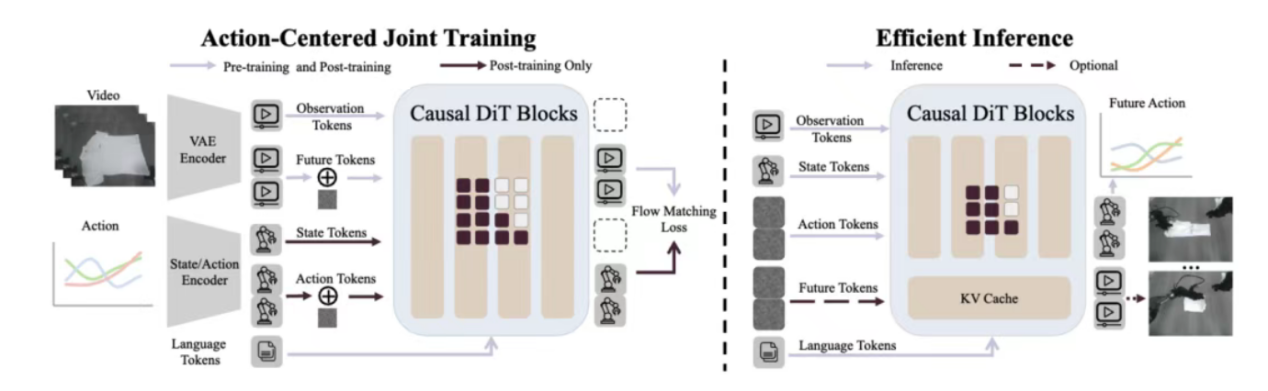
\includegraphics{images/image-0049.png}
\caption{GigaWorld-Policy 的动作中心联合训练与高效推理示意图}
\end{figure}

\hypertarget{ux4e8cux3c00.7vlaux6a21ux578b}{%
\subsubsection{（二）π0.7（VLA模型）}\label{ux4e8cux3c00.7vlaux6a21ux578b}}

π0.7涌现出组合泛化能力的关键在于，用多样化的prompt处理多样化的数据。过去VLA训练只喂一句清理冰箱，模型得到的信号是单一的。π0.7把prompt展开成四层：任务指令（清理厨房）+子任务指令（打开冰箱）+子目标图像（下一秒画面应该长什么样）+episode元数据（这条数据质量几分、有没有出错、速度多快）。

有了这些丰富的context，模型就能分得清训练数据里的好坏、快慢、对错。然后它就能吃下以前吃不了的数据。失败的rollouts，低质量的演示，其他机器人的片段，人类的egocentric视频，全都变成有用的信号。简而言之，π0.7加的那层prompt，就是让模型知道``这段数据是什么质量、用什么策略做的''。

\hypertarget{ux4e09ux9ad8ux5fb7abot-3dgsabot-physworldworld-modelux4f5cux4e3aux8badux7ec3ux73afux5883}{%
\subsubsection{（三）高德ABot-3DGS、ABot-PhysWorld（World Model作为训练环境）}\label{ux4e09ux9ad8ux5fb7abot-3dgsabot-physworldworld-modelux4f5cux4e3aux8badux7ec3ux73afux5883}}

先把数据转成机器能读懂的``多模态Clip''，比如骑车经过一个路口，高德记录下来的不只是一张图，而是一整套信息，包括路口长什么样（图像）、红绿灯在哪（空间位置）、现在是红灯还是绿灯（状态）、你是直行还是准备转弯（行为），甚至还包括周围有没有行人、车辆在动等，所有东西打包在一起就是一个Clip。ABot-3DGS利用这些Clip数据，重建3D真实场景；ABot-PhysWorld在这些场景中进行合乎物理定律（如滑动、倾倒、堆叠、流体变化）的动作推演。

对于ABot-PhysWorld的训练数据，高德精选300万条真实操作视频，用VLM+LLM双阶段标注，构建四层级物理语义结构，将数据拆解成机器人更易``消化''的结构化信息：

宏观层（意图）：自然语言描述整体任务目标，如``抓取并放置苹果''。

中观层（动作序列）：动词-名词短语序列，如``接近→抓握→提起→移动→释放''。

微观层（轨迹细节）：记录笛卡尔轨迹、相对运动、夹爪状态，如``末端沿Z轴下降5cm，夹爪闭合至20mm''。

场景层（物理关系）：描述接触、支撑、包含关系及任务结果，如``苹果与桌面接触，被夹爪稳固抓握，成功放置于袋中''。

这套标注流程不仅在告诉机器人``发生了什么''，更在解释``为什么发生''。

\hypertarget{ux53c2ux8003ux6587ux732e-172}{%
\subsection{参考文献}\label{ux53c2ux8003ux6587ux732e-172}}

\begin{itemize}
\tightlist
\item
  O'Neill, A., Rehman, A., Gupta, A., et al.~(2024). \href{https://arxiv.org/abs/2310.08864}{Open X-Embodiment: Robotic Learning Datasets and RT-X Models}. ICRA.
\item
  Walke, H., Black, K., Lee, A., et al.~(2023). \href{https://arxiv.org/abs/2308.12952}{BridgeData V2: A Dataset for Robot Learning at Scale}. arXiv:2308.12952.
\item
  Ye, A., Wang, B., Ni, C., et al.~(2026). \href{https://arxiv.org/abs/2603.17240}{GigaWorld-Policy: An Efficient Action-Centered World--Action Model}. arXiv:2603.17240.
\item
  Physical Intelligence, Ai, B., Amin, A., Aniceto, R., et al.~(2026). \href{https://arxiv.org/abs/2604.15483}{\(\pi_{0.7}\): a Steerable Generalist Robotic Foundation Model with Emergent Capabilities}. arXiv:2604.15483.
\item
  Yang, Y., Zeng, S., Lin, T., et al.~(2026). \href{https://arxiv.org/abs/2602.11236}{ABot-M0: VLA Foundation Model for Robotic Manipulation with Action Manifold Learning}. arXiv:2602.11236.
\item
  AMAP CV Lab. (2026). \href{https://amap-cvlab.github.io/ABot-Manipulation/}{ABot-M0: VLA Foundation Model for Robotic Manipulation with Action Manifold Learning}.
\item
  量子位. (2026). \href{https://www.traeai.com/articles/e175141a-e8b5-4e06-a589-42bd432aa115}{高德发布全球首个面向AGI的全栈具身技术体系``ABot''：15项SOTA，构建持续进化的具身智能闭环}.
\end{itemize}

\clearpage

\hypertarget{ux7b56ux7565ux51fdux6570ux7684ux8badux7ec3ux65b9ux6cd5}{%
\section{策略函数的训练方法}\label{ux7b56ux7565ux51fdux6570ux7684ux8badux7ec3ux65b9ux6cd5}}

在具身智能中，运动控制策略函数（即``小脑''）的训练是关键。

\hypertarget{ux4e00ux57faux4e8eux7ecfux5178ux63a7ux5236ux7406ux8bba}{%
\subsection{一、基于经典控制理论}\label{ux4e00ux57faux4e8eux7ecfux5178ux63a7ux5236ux7406ux8bba}}

这是最传统的机器人控制方法。

\begin{itemize}
\tightlist
\item
  核心逻辑：基于机器人的精确动力学方程（如拉格朗日动力学），在未来有限的时间窗口内，通过求解一个带约束的凸优化或非线性优化问题，计算出当前的最佳电机力矩。
\item
  数学建模：
\end{itemize}

假设``大脑''给出了未来 \(N\) 步的参考状态轨迹 \(x_k^{ref}\)，MPC``小脑''需要在满足动力学约束和不等式约束（如电机最大扭矩 \(u_{max}\)、足端接触摩擦锥限制）的前提下，最小化跟踪误差和能量消耗：

\[
\min_{u_{0:N-1}}
\sum_{k=0}^{N-1}
\left(
\|x_k-x_k^{ref}\|_Q^2+\|u_k\|_R^2
\right)
+
\|x_N-x_N^{ref}\|_{Q_f}^2
\]

\[
\text{s.t.}\quad x_{k+1}=f(x_k,u_k)\quad \mathcjk{（\mathcjk{刚体动力学}）}
\]

\[
h(x_k,u_k)\le 0\quad \mathcjk{（\mathcjk{物理与防碰撞约束}）}
\]

\begin{itemize}
\tightlist
\item
  工作流：

  \begin{enumerate}
  \def\labelenumi{\arabic{enumi}.}
  \tightlist
  \item
    指令接收：接收大脑下发的粗糙目标，如``向前走 1 米''或具体的足端落点。
  \item
    运动学与动力学建模：系统实时更新雅可比矩阵（Jacobian）和惯性矩阵。
  \item
    实时优化求解：利用二次规划（QP）求解器或非线性求解器（如基于牛顿法的内点法），以极高的频率（如 500Hz）实时计算出上述优化问题的解 \(u_0^*\)。
  \item
    力矩下发：将计算出的第一个控制指令 \(u_0^*\) 转换为电流信号，驱动底层伺服电机，并在下一个控制周期滚动重复此过程。
  \end{enumerate}
\end{itemize}

\hypertarget{ux4e8cux6a21ux4effux5b66ux4e60}{%
\subsection{二、模仿学习}\label{ux4e8cux6a21ux4effux5b66ux4e60}}

对于机械臂抓取、灵巧手操作等依赖高维视觉输入且难以设计密集奖励函数（Dense Reward）的任务，模仿学习是目前训练``小脑''的最前沿路线。近年来，基于扩散策略（Diffusion Policy）和动作分块（Action Chunking，如 ACT）的方法占据了统治地位。

\begin{itemize}
\tightlist
\item
  核心逻辑：跳过奖励函数的试错，直接利用神经网络拟合人类专家遥操作（Teleoperation）产生的高质量演示数据。
\item
  数学建模（以 Diffusion Policy 为例）：
\end{itemize}

扩散模型不再输出单一的确定动作，而是将动作生成建模为从随机噪声中逐步去噪的过程。给定大脑的指令 \(g\) 和当前的视觉/本体观测 \(o_t\)，模型预测一段未来连续步的动作轨迹序列 \(\mathbf{a}_{t:t+H}\)。其核心是训练一个条件噪声预测网络 \(\epsilon_\theta\)，最小化去噪过程的均方误差：

\[
\begin{aligned}
\mathcal{L}
&=
\mathbb{E}_{\mathbf{a}^0\sim\mathcal{D},\epsilon\sim\mathcal{N}(0,I),k}
\left[
\left\|
\epsilon-\epsilon_\theta(\mathbf{a}^k,o_t,g,k)
\right\|_2^2
\right]
\end{aligned}
\]

其中 \(\mathbf{a}^0\) 是真实的专家动作序列，\(\mathbf{a}^k\) 是加了 \(k\) 步前向高斯噪声的动作，\(\epsilon\) 是实际添加的噪声。

计算的是真实噪声与网络预测噪声之间的均方误差（MSE）。

公式中各项含义如下：

\begin{itemize}
\tightlist
\item
  \(\mathcal{L}\)：整体的损失函数。
\item
  \(\mathbb{E}\)：期望符号，代表在训练时对下标中的变量进行随机采样，并计算均值。
\item
  \(\mathbf{a}^0\sim\mathcal{D}\)：从人类专家示教数据集 \(\mathcal{D}\) 中采样出的真实动作序列（Ground Truth）。上标 0 代表这是未受任何污染的原始干净动作。在动作分块（Action Chunking）架构下，它通常不是单个动作，而是一段未来序列，例如未来 16 步的关节力矩向量。
\item
  \(\epsilon\sim\mathcal{N}(0,I)\)：从标准正态分布中采样出的真实高斯噪声。
\item
  \(k\)：扩散过程的时间步（Diffusion Step），通常从 1 到 \(K\)（例如 \(K=100\)）中均匀随机采样。
\item
  \(\mathbf{a}^k\)：带噪动作序列。它是将真实动作 \(\mathbf{a}^0\) 加上第 \(k\) 步对应强度的噪声 \(\epsilon\) 后得到的结果。\(k\) 越大，\(\mathbf{a}^k\) 越接近纯噪声。
\item
  \(o_t,g\)：条件变量（Conditions）。\(o_t\) 是机器人当前时刻的物理观测，如相机图像、本体关节角度；\(g\) 是语言指令或全局任务目标。
\item
  \(\epsilon_\theta(\cdot)\)：需要训练的神经网络，通常是带有交叉注意力机制的 1D U-Net 或 Transformer。\(\theta\) 是网络权重。它的输入是带噪动作 \(\mathbf{a}^k\) 以及条件变量，输出是它猜测的当初加进 \(\mathbf{a}^k\) 里的噪声 \(\epsilon\)。
\item
  \(\|\cdot\|_2^2\)：L2 范数的平方，即要求网络预测的噪声与实际添加的噪声尽可能一致。
\end{itemize}

工作流：

\begin{enumerate}
\def\labelenumi{\arabic{enumi}.}
\tightlist
\item
  数据采集：操作员使用动捕设备或 VR 手柄，在真实环境或仿真环境中控制机器人完成特定任务，记录下 \((o_t,g_t,a_t)\) 的轨迹对。
\item
  噪声注入与模型训练：在训练阶段，对专家动作序列注入不同时间步的高斯噪声。利用基于 CNN 或 Transformer 的 U-Net 架构，以视觉特征和指令特征作为条件（Condition），训练模型预测注入的噪声。
\item
  闭环推理执行：在实际部署时，模型接收实时观测，从纯高斯噪声开始，经过多步迭代去噪（如 DDIM 采样），生成一条平滑的未来动作轨迹。执行该轨迹的前几步后，重新观测环境并生成新轨迹（Receding Horizon Control）。
\end{enumerate}

\hypertarget{ux4e09ux5f3aux5316ux5b66ux4e60}{%
\subsection{三、强化学习}\label{ux4e09ux5f3aux5316ux5b66ux4e60}}

模仿学习具有显著的局限性，具身智能不能只会模仿人类，而是要能在探索中自主学习。因而强化学习是目前具身智能领域的核心和前沿，尤其擅长处理非线性动力学和复杂的环境接触。

``小脑''的策略被定义为参数化的概率分布 \(\pi_\theta(a_t|s_t,g_t)\)，其中 \(s_t\) 是本体感受器状态（如关节位置、IMU 数据），\(g_t\) 是大脑下发的子目标（如目标速度、目标位姿），\(a_t\) 是底层控制指令。

以 SAC 为例，其优化的目标函数不仅最大化累计奖励，还最大化策略的熵 \(\mathcal{H}\)，以鼓励探索并提升鲁棒性：

\[
\begin{aligned}
J(\pi_\theta)
&=
\mathbb{E}_{\tau\sim\pi_\theta}
\left[
\sum_{t=0}^{T}
\gamma^t
\left(
r(s_t,a_t,g_t)+
\alpha\mathcal{H}(\pi_\theta(\cdot|s_t,g_t))
\right)
\right]
\end{aligned}
\]

工作流（Sim2Real 范式）：

\begin{enumerate}
\def\labelenumi{\arabic{enumi}.}
\tightlist
\item
  仿真环境构建：在 Isaac Gym 或 MuJoCo 等高精度物理仿真器中建立机器人的数字孪生。
\item
  域随机化（Domain Randomization）：为了跨越``仿真到现实''（Sim2Real）的鸿沟，在训练时对物理参数（质量、摩擦系数、电机延迟、传感器噪声等）进行大幅度的随机采样。
\item
  大规模并行训练：利用 GPU 并行运行成千上万个环境，通过 PPO/SAC 算法收集轨迹数据，更新 Actor 网络（即``小脑''策略）和 Critic 网络。
\item
  真机部署（zero-shot Transfer）：将训练好的 Actor 网络权重直接冻结并部署到真实机器人控制器上，根据实时状态和大脑指令输出动作。
\end{enumerate}

强化学习的难点在于，需要在环境中试错，真机训练成本极为高昂。一种方法是引入基于世界模型的强化学习。以VLAW为例：

\begin{enumerate}
\def\labelenumi{\arabic{enumi}.}
\tightlist
\item
  收集真实世界数据：让 VLA 策略在真实世界中执行，收集少量包含成功与失败的轨迹数据，并标注离散的成功/失败奖励。
\item
  后训练世界模型与奖励模型：将收集到的真实轨迹数据与原始的机器人操作数据集结合，共同训练并微调预训练的世界模型，以防止模型对少量数据过拟合并提升其在特定任务上的物理准确性。同时，使用首轮真实数据微调视觉-语言奖励模型（Qwen3-VL-4B-Instruct），以提高奖励评估的保守度与准确性。
\item
  生成带奖励标签的合成轨迹：在更新后的世界模型中运行 VLA 策略，闭环自回归地生成大量合成轨迹。随后，利用预设好概率阈值的奖励模型对这些虚拟轨迹进行过滤，保留判定为成功的样本。
\item
  后训练 VLA 策略：整合过滤后的成功真实轨迹与成功合成轨迹，给成功轨迹分配权重 1，失败轨迹分配权重 0，使用流匹配（Flow-matching）目标函数对 VLA 策略进行更新。
\item
  循环迭代：交替重复上述步骤，不断协同提升世界模型和 VLA 策略的性能。
\end{enumerate}

后续内容会介绍世界模型与具身智能的具体结合方式。

\hypertarget{ux53c2ux8003ux6587ux732e-173}{%
\subsection{参考文献}\label{ux53c2ux8003ux6587ux732e-173}}

\begin{itemize}
\tightlist
\item
  Chi, C., Feng, S., Du, Y., Xu, Z., Cousineau, E., Burchfiel, B., \& Song, S. (2023). \href{https://arxiv.org/abs/2303.04137}{Diffusion Policy: Visuomotor Policy Learning via Action Diffusion}. RSS.
\item
  Zhao, T. Z., Kumar, V., Levine, S., \& Finn, C. (2023). \href{https://arxiv.org/abs/2304.13705}{Learning Fine-Grained Bimanual Manipulation with Low-Cost Hardware}. RSS.
\end{itemize}

\clearpage

\hypertarget{vlaux6a21ux578b}{%
\section{VLA模型}\label{vlaux6a21ux578b}}

VLA（Vision-Language-Action，视觉-语言-动作）模型正在引发一场范式革命，它打破了传统机器人``感知-规划-控制''的模块化割裂设计，将多模态大模型的语义推理能力直接映射为物理世界的底层执行动作。

\hypertarget{ux4e00ux6838ux5fc3ux601dux60f3-20}{%
\subsection{一、核心思想}\label{ux4e00ux6838ux5fc3ux601dux60f3-20}}

VLA模型的核心思想是``端到端''（End-to-End）的多模态深度融合。它将预训练的视觉-语言模型（VLM）作为``大脑''，把机器人的动作输出转化为一种特殊的``语言''，从而让大模型能够直接指挥物理硬件。

视觉（Vision）：通过视觉编码器（如ViT、SigLIP）将输入图像（如RGB摄像机画面流）切分为Patch，并转化为视觉Token，赋予机器人理解空间关系、物理属性的能力。

语言（Language）：接收人类的自然语言指令，结合预训练大模型积累的庞大互联网知识，提供逻辑推理与``常识''。

动作（Action）：VLA将动作词表化，将连续的机器人物理控制参数（如机械臂的关节扭矩、末端执行器的坐标）离散化，作为一种特殊的Token融入大语言模型的词表中。

\hypertarget{ux4e8cux81eaux56deux5f52vlaux8303ux5f0f}{%
\subsection{二、自回归VLA范式}\label{ux4e8cux81eaux56deux5f52vlaux8303ux5f0f}}

\hypertarget{ux4e00ux57faux672cux539fux7406-2}{%
\subsubsection{（一）基本原理}\label{ux4e00ux57faux672cux539fux7406-2}}

假设在时间步 \(t\)，智能体接收到视觉观测序列 \(o_{\le t}\in\mathcal{O}\) 以及自然语言指令 \(l\in\mathcal{L}\)，模型的目标是输出最优动作 \(a_t\in\mathcal{A}\)。

在以 RT-2（Robotic Transformer 2）和 OpenVLA 为代表的自回归（Autoregressive）VLA 范式中，连续动作 \(a_t\) 会被离散化为一系列动作 Token \((z_1,z_2,\ldots,z_K)\)。例如，一个 7 自由度（7-DoF）的机械臂动作可以表示为空间位移、旋转和夹爪开合度。

模型的训练目标是最大化以观测和指令为条件的动作 Token 的对数似然（Log-Likelihood）：

\[
\begin{aligned}
\mathcal{J}(\theta)
&=
\mathbb{E}_{(o,l,a)\sim\mathcal{D}}
\left[
\sum_{k=1}^{K}
\log P_{\theta}(z_k\mid z_{<k}, o_{\le t}, l)
\right]
\end{aligned}
\]

其中，\(\theta\) 为神经网络的参数，\(\mathcal{D}\) 为包含人类专家示范和互联网图文的混合数据集。通过这种方式，动作预测被完全等价转化为了类似于 ChatGPT 生成文本的 Next-token Prediction 任务。

\hypertarget{ux4e8cux5de5ux4f5cux6d41-6}{%
\subsubsection{（二）工作流}\label{ux4e8cux5de5ux4f5cux6d41-6}}

\begin{enumerate}
\def\labelenumi{\arabic{enumi}.}
\item
  多模态输入处理（Multimodal Input Processing）：步骤 1.1，获取当前相机的 RGB 图像 \(o_t\)，通过视觉编码器（Vision Encoder）提取特征，并经过 Projector（投影层）对齐到语言模型的特征空间，生成视觉 Token 序列；步骤 1.2，接收用户指令 \(l\)，通过文本分词器生成语言 Token 序列。
\item
  特征拼接与跨模态注意力计算（Context Concatenation \& Cross-modal Attention）：步骤 2.1，将系统提示词、视觉 Token 和语言 Token 按序列拼接为 \texttt{{[}System\ Prompt,\ Image\ Tokens,\ Language\ Tokens{]}}；步骤 2.2，送入 Transformer Decoder 骨干网络，通过自注意力机制（Self-Attention）让指令语义与图像中的物理特征产生深度绑定（Grounding）。
\item
  自回归动作生成（Autoregressive Action Generation）：步骤 3.1，Transformer 结合上下文，逐个预测当前步骤的动作 Token。例如先预测代表 \(A_x\) 的 Token，再将 \(A_x\) 作为已知条件预测 \(A_y\)，依次类推，直到输出夹爪动作 Token。
\item
  反词表化与物理控制（Detokenization and Execution）：步骤 4.1，将生成的动作 Token 序列 \((z_1,\ldots,z_K)\) 映射回连续的物理数值，生成实际控制指令；步骤 4.2，将指令发送给机器人底层控制器（如 PID 控制器）驱动电机执行。
\end{enumerate}

\hypertarget{ux4e09ux4f18ux7f3aux70b9}{%
\subsubsection{（三）优缺点}\label{ux4e09ux4f18ux7f3aux70b9}}

自回归VLA直接复用LLM的架构，天然继承了互联网级数据的逻辑链条（Chain-of-Thought）和常识推理能力。泛化能力极强，但受限于自回归的生成速度，高频连续控制能力略显不足。

\hypertarget{ux4e09ux6269ux6563ux6d41ux5339ux914dvlaux8303ux5f0f}{%
\subsection{三、扩散/流匹配VLA范式}\label{ux4e09ux6269ux6563ux6d41ux5339ux914dvlaux8303ux5f0f}}

这一范式的核心动机是消除``动作词表化''带来的离散化误差。它不再将动作强行转化为语言词表中的 Token，而是使用生成式连续时间模型（Diffusion Models 或 Flow Matching）直接在连续空间中生成高维、高频的动作轨迹（Action Chunks）。代表性模型包括 Physical Intelligence 的 \(\pi_0\)（Pi-Zero）、ForceVLA 等。

扩散/流匹配 VLA 通常采用 \textbf{``VLM + 动作专家（Action Expert）''} 的解耦与重组架构：

\begin{enumerate}
\def\labelenumi{\arabic{enumi}.}
\item
  多模态条件编码器：继承预训练的视觉语言模型（如 PaliGemma、SigLIP 结合 LLM 骨干），负责将图像序列 \(o\) 和语言指令 \(l\) 处理为深度的上下文条件嵌入（Condition Embeddings）。
\item
  连续动作生成器（Action Expert）：通常是 Diffusion Transformer（DiT）或 U-Net，接收上述条件嵌入，并通过交叉注意力机制（Cross-Attention）或拼接自注意力机制，对纯噪声信号进行迭代去噪，最终输出连续的物理动作块 \(A_t=(a_t,a_{t+1},\ldots,a_{t+H-1})\)。
\end{enumerate}

以目前先进的最优传输流匹配（Optimal Transport Flow Matching，类似于 \(\pi_0\) 中的设计）为例。假设基础噪声分布为 \(x_0\sim p_0=\mathcal{N}(0,I)\)，真实动作轨迹分布为 \(x_1\sim p_1\)，多模态条件为 \(c=\mathrm{Encoder}(o,l)\)。模型构建一条连接噪声与真实动作的直线概率路径：

\[
x_t=(1-t)x_0+t x_1
\]

动作生成器 \(v_\theta\) 的目标是拟合真实的速度场（Velocity Field），其目标函数定义为：

\[
\begin{aligned}
\mathcal{L}_{\mathrm{FM}}(\theta)
&=
\mathbb{E}_{\substack{t\sim \mathcal{U}(0,1)\\ x_0\sim p_0,\ x_1\sim p_1}}
\left[
\left\|v_\theta(x_t,t,c)-(x_1-x_0)\right\|^2
\right]
\end{aligned}
\]

这里 \((x_1-x_0)\) 是真实路径的恒定梯度。相较于传统的 DDPM 扩散模型，流匹配的 ODE 轨迹更加平滑且笔直，能够在极少的推理步数（甚至几步内）生成高保真的连续动作信号。
工作流：

\begin{enumerate}
\def\labelenumi{\arabic{enumi}.}
\item
  特征提取：VLM 接收当前相机观测和语言 \(l\)，前向传播生成多模态条件向量 \(c\)。
\item
  噪声初始化：从标准正态分布中采样一段长度为 \(H\) 的纯噪声轨迹 \(x_0\sim\mathcal{N}(0,I)\)。
\item
  常微分方程求解（ODE Solving）：在时间步 \(t\in[0,1]\) 之间，动作生成器 \(v_\theta(x_t,t,c)\) 结合上下文 \(c\) 计算当前状态的梯度，并通过数值积分器（如 Euler 法或 Heun 法）逐步更新。
\item
  动作执行：将 ODE 终点作为预测的动作块。系统采用模型预测控制（MPC/Receding Horizon Control）策略，仅执行前几个动作，随后重新获取新的视觉观测，进入下一轮闭环推理。
  优缺点：动作输出不再是离散 Token，而是通过 Diffusion Model（扩散模型）或 Flow Matching 直接生成连续的动作轨迹，在处理需要极高精度和灵巧度（如折叠衣服、灵巧手操作）的任务时表现出显著优势，但在长程任务的因果关系保持上可能不如自回归。
\end{enumerate}

\hypertarget{ux56dbux7edfux4e00ux8868ux5f81ux4e0eux6f5cux5728ux52a8ux4f5cux8303ux5f0f}{%
\subsection{四、统一表征与潜在动作范式}\label{ux56dbux7edfux4e00ux8868ux5f81ux4e0eux6f5cux5728ux52a8ux4f5cux8303ux5f0f}}

不同机器人的硬件形态之间（乃至与人类第一视角之间）存在差异。为了让VLA模型不被限制于特定的硬件中，而是可以利用海量无动作标签的视频进行扩展（Scaling），我们引入``抓取右上方的物体''等与具体硬件无关的统一潜在动作，而不是``右臂上抬30厘米''这样的具体机械操作。

在具身智能架构分类中，它介于分层和端到端之间，因为模型间传递的信息是可微的，梯度可以（在某些设计下）从底层直接传导回高层，或者在同一个世界模型的潜空间内完成对齐。

\hypertarget{ux4e00ux6838ux5fc3ux67b6ux6784-7}{%
\subsubsection{（一）核心架构}\label{ux4e00ux6838ux5fc3ux67b6ux6784-7}}

该路线的核心架构仍可拆成两部分：多模态条件编码器继承预训练的 VLM，将图像序列 \(o\) 与语言指令 \(l\) 编码为上下文条件嵌入；连续动作生成器接收这些条件嵌入，生成统一潜在动作块 \(A_t=(a_t,a_{t+1},\ldots,a_{t+H-1})\)。区别在于，高层输出的并不一定是某个机器人专属的底层控制量，而是可跨形态共享的潜在动作表示。

\hypertarget{ux4e8cux8badux7ec3ux65b9ux6cd5-1}{%
\subsubsection{（二）训练方法}\label{ux4e8cux8badux7ec3ux65b9ux6cd5-1}}

\begin{enumerate}
\def\labelenumi{\arabic{enumi}.}
\tightlist
\item
  训练阶段一：潜在动作空间的无监督学习（Latent Action Learning）。这一阶段不需要任何底层物理控制信号（如关节扭矩），模型仅通过观看海量视频序列来学习。模型通常引入一个基于 VQ-VAE（向量量化变分自编码器）的逆动力学模型（Inverse Dynamics Model）：输入连续两帧视频图像 \((o_t,o_{t+1})\)，编码器提取两帧之间的视觉和物理状态变化，生成连续隐特征；向量量化模块将连续隐特征映射到离散密码本（Codebook）中，提取以任务为中心的潜在动作 \(z_t\)；前向动力学模型接收当前帧 \(o_t\) 和潜在动作 \(z_t\)，尝试重建下一帧图像 \(\hat{o}_{t+1}\)。
\end{enumerate}

损失函数由重建损失和密码本正则化损失组成：

\[
\begin{aligned}
\mathcal{L}_{\mathrm{VQ}}
&= \|o_{t+1}-\hat{o}_{t+1}\|^2
+\|\mathrm{sg}[\mathrm{Encoder}(o_t,o_{t+1})]-e_{z_t}\|^2
\\
&\quad+
\beta\|\mathrm{Encoder}(o_t,o_{t+1})-\mathrm{sg}[e_{z_t}]\|^2
\end{aligned}
\]

其中，\(e_{z_t}\) 为密码本中的嵌入向量，\(\mathrm{sg}[\cdot]\) 为停止梯度操作。

\begin{enumerate}
\def\labelenumi{\arabic{enumi}.}
\setcounter{enumi}{1}
\tightlist
\item
  训练阶段二：联合策略优化与具身对齐（Joint Policy Optimization）。在获得跨形态潜在动作空间后，开始正式训练 VLA 大模型，将语义与物理硬件绑定。首先利用阶段一训练好的 VQ-VAE 编码器，把带有语言指令的机器人视频数据转化为``指令-图像-潜在动作 \(z_t\)''的离散序列数据；然后用标准的 Next-token Prediction 目标训练 VLM 主干网络，使其在给定图像和文本上下文时输出正确的潜在动作分布 \(P_\theta(z_t\mid o_{\le t},l)\)；最后引入轻量级形态感知解码器（Embodiment-aware Decoder）或联合扩散模块，将 VLM 输出的潜在动作 \(z_t\) 与当前机器人的专属形态标识拼接，并使用少量包含真实底层动作标签的数据训练该解码器：
\end{enumerate}

\[
\begin{aligned}
\mathcal{L}_{\mathrm{Action}}
&=
\mathbb{E}\left[
-\log P_\phi(a_t\mid z_t,o_t,\text{embodiment\_id})
\right]
\end{aligned}
\]

其中，目前业界部分实践在高层运用自回归以适配成熟生态，底层运用扩散以降低延迟。

\hypertarget{ux53c2ux8003ux6587ux732e-174}{%
\subsection{参考文献}\label{ux53c2ux8003ux6587ux732e-174}}

\begin{itemize}
\tightlist
\item
  Brohan, A., Brown, N., Carbajal, J., et al.~(2023). \href{https://arxiv.org/abs/2307.15818}{RT-2: Vision-Language-Action Models Transfer Web Knowledge to Robotic Control}. arXiv:2307.15818.
\item
  Kim, M. J., Pertsch, K., Karamcheti, S., et al.~(2024). \href{https://arxiv.org/abs/2406.09246}{OpenVLA: An Open-Source Vision-Language-Action Model}. arXiv:2406.09246.
\item
  Black, K., Brown, N., Driess, D., et al.~(2024). \href{https://arxiv.org/abs/2410.24164}{π0: A Vision-Language-Action Flow Model for General Robot Control}. arXiv:2410.24164.
\end{itemize}

\clearpage

\hypertarget{ux5177ux8eabux667aux80fdux7684ux672aux6765ux5c55ux671b}{%
\section{具身智能的未来展望}\label{ux5177ux8eabux667aux80fdux7684ux672aux6765ux5c55ux671b}}

大语言模型诞生后，AI在数字世界快速发展；具身智能则意味着AI向物理世界的拓展。下面是对未来具身智能发展的一些展望。

\hypertarget{ux4e00ux5177ux8eabux667aux80fdux7684ux57faux672cux5f62ux6001ux5c55ux671b}{%
\subsection{一、具身智能的基本形态展望}\label{ux4e00ux5177ux8eabux667aux80fdux7684ux57faux672cux5f62ux6001ux5c55ux671b}}

未来，我们希望基于具身智能的机器人能在足够丰富、足够复杂的现实任务里，像人类一样完成工作。这里引入``物理图灵测试''的概念，即人类已经无法仅靠观察去判断完成工作的是人类还是机器人。进一步来说，具身智能未来将不是独立的机器，而可以通过API或其他更高级的方式被调用。

\hypertarget{ux4e8cux5177ux8eabux667aux80fdux7684ux4e0bux6e38ux5e94ux7528ux5c55ux671b}{%
\subsection{二、具身智能的下游应用展望}\label{ux4e8cux5177ux8eabux667aux80fdux7684ux4e0bux6e38ux5e94ux7528ux5c55ux671b}}

在日常生活层面，具身智能将承担家务、照护、陪伴和家庭维修等任务。它不只是会执行固定动作的家电，而是能理解家庭成员的真实需求，感知复杂环境中的物品、老人、儿童和宠物状态，并在安全边界内自主规划行动，例如整理房间、准备餐食、照看老人、处理突发情况等。

在服务业层面，具身智能将进入餐饮、酒店、物流、医疗护理、零售和公共服务等场景。未来的机器人不仅能完成送餐、清洁、搬运、导览等重复性工作，也能根据顾客的语言、表情和行为作出灵活回应，从而让服务更稳定、更低成本，也让人类员工从高强度、低创造性的劳动中解放出来。

在工业层面，具身智能将实现工业生产的无人化。未来人类以自然语言等形式描述的需求可交由大模型得到可执行的生产方案，而实体生产过程可以完全由机器人自主完成。机器人可以操控流水线上的机器、监控生产状态，并对紧急状况及时作出反应。

在农业层面，具身智能将推动农业从依赖经验和人工劳动，走向精准化、自动化和数据化。机器人可以完成播种、除草、施肥、采摘、病虫害识别、土壤监测和农作物分拣等任务，并根据天气、土壤、水分和作物生长状态实时调整策略，从而提高产量、减少浪费，也缓解农业劳动力不足的问题。

在科学研究层面，如对于生物学中的临床样本处理、肿瘤切片、动物实验、复杂组织培养，以及执行全新实验流程、故障排错等硬编码难以处理的场景，具身智能可以将科学家从繁重的实验中解放出来，使其进行创造性思考而不是反复重做实验，并实现更多实验的标准化和数据统一，让AI Scientist从``窄域工业化闭环''走向``通用科学家闭环''。

\hypertarget{ux4e09ux5177ux8eabux667aux80fdux63a8ux52a8ux81eaux8eab}{%
\subsection{三、具身智能推动自身}\label{ux4e09ux5177ux8eabux667aux80fdux63a8ux52a8ux81eaux8eab}}

有认知理论认为，真正的智能的形成需要依赖与环境的互动。具身智能将能在现实世界大规模执行任务的同时，收集视觉、语言、传感器信号、环境状态变化等数据。结合这些交互数据训练模型，特别是结合带有``干预动作-状态转移''的因果数据和互联网视频难以触及的长尾数据训练模型，能让模型更好地理解物理世界及其因果关系，让模型具备真正意义上完全达到乃至超过人类水平的通用智能。

此外，机器人还可以自主设计、优化和制造下一代机器人，实现``Robots for robots''，极大地加速迭代。未来或许还将有为更多环境、更多用途打造的机器人，如纳米机器人、太空探索机器人、深海作业机器人、灾害救援机器人、极端环境维修机器人等。它们将把AI的能力从屏幕和服务器扩展到真实世界，使智能系统不只是``思考''和``生成''，而是能够真正行动、制造、探索和改变环境。

\hypertarget{ux53c2ux8003ux6587ux732e-175}{%
\subsection{参考文献}\label{ux53c2ux8003ux6587ux732e-175}}

\begin{itemize}
\tightlist
\item
  Varela, F. J., Thompson, E., \& Rosch, E. (2017). \href{https://mitpress.mit.edu/9780262529365/the-embodied-mind/}{The Embodied Mind: Cognitive Science and Human Experience} (Revised ed.). MIT Press. (Original work published 1991).
\item
  Brooks, R. A. (1991). \href{https://doi.org/10.1016/0004-3702\%2891\%2990053-M}{Intelligence without representation}. \emph{Artificial Intelligence}, 47(1-3), 139-159.
\item
  Sequoia Capital. (2025). \href{https://www.youtube.com/watch?v=_2NijXqBESI}{The Physical Turing Test: Jim Fan on Nvidia's Roadmap for Embodied AI}. YouTube.
\item
  Zhu, Y., Fan, L., \& NVIDIA GEAR Team. (2025). \href{https://research.nvidia.com/publication/2025-03_nvidia-isaac-gr00t-n1-open-foundation-model-humanoid-robots}{NVIDIA Isaac GR00T N1: An Open Foundation Model for Humanoid Robots}. NVIDIA Research.
\item
  Google DeepMind. (2025). \href{https://deepmind.google/models/gemini-robotics/}{Gemini Robotics}.
\item
  Brohan, A., Brown, N., Carbajal, J., et al.~(2023). \href{https://arxiv.org/abs/2307.15818}{RT-2: Vision-Language-Action Models Transfer Web Knowledge to Robotic Control}. arXiv:2307.15818.
\item
  O'Neill, A., Rehman, A., Gupta, A., et al.~(2024). \href{https://arxiv.org/abs/2310.08864}{Open X-Embodiment: Robotic Learning Datasets and RT-X Models}. ICRA.
\item
  Black, K., Brown, N., Driess, D., et al.~(2024). \href{https://arxiv.org/abs/2410.24164}{π0: A Vision-Language-Action Flow Model for General Robot Control}. arXiv:2410.24164.
\item
  Bousmalis, K., Vezzani, G., Rao, D., et al.~(2023). \href{https://arxiv.org/abs/2306.11706}{RoboCat: A Self-Improving Generalist Agent for Robotic Manipulation}. arXiv:2306.11706.
\item
  Lu, C., Lu, C., Lange, R. T., Foerster, J., Clune, J., \& Ha, D. (2024). \href{https://arxiv.org/abs/2408.06292}{The AI Scientist: Towards Fully Automated Open-Ended Scientific Discovery}. arXiv:2408.06292.
\end{itemize}

\clearpage


% 多模态生成与生成式世界模型
\hypertarget{ux591aux6a21ux6001ux751fux6210ux4e0eux751fux6210ux5f0fux4e16ux754cux6a21ux578b}{%
\chapter{多模态生成与生成式世界模型}\label{ux591aux6a21ux6001ux751fux6210ux4e0eux751fux6210ux5f0fux4e16ux754cux6a21ux578b}}

\hypertarget{ux81eaux56deux5f52ux6269ux6563ux7684ux7ed3ux5408ux4e0eux65f6ux7a7atransformer}{%
\section{自回归、扩散的结合与时空Transformer}\label{ux81eaux56deux5f52ux6269ux6563ux7684ux7ed3ux5408ux4e0eux65f6ux7a7atransformer}}

\hypertarget{ux4e00ux81eaux56deux5f52ux751fux6210ux7684ux4e16ux754cux6a21ux578b}{%
\subsection{一、自回归生成的世界模型}\label{ux4e00ux81eaux56deux5f52ux751fux6210ux7684ux4e16ux754cux6a21ux578b}}

\hypertarget{ux4e00ux81eaux56deux5f52ux751fux6210ux8303ux5f0fux4ee5genie-1ux4e3aux4f8b}{%
\subsubsection{（一）自回归生成范式：以Genie 1为例}\label{ux4e00ux81eaux56deux5f52ux751fux6210ux8303ux5f0fux4ee5genie-1ux4e3aux4f8b}}

下面以Genie 1为例，介绍自回归生成的经典范式，及其核心架构（如时空Transformer等）。

训练阶段（Training Phase）：

\begin{enumerate}
\def\labelenumi{\arabic{enumi}.}
\item
  首先，单独训练视频分词器（Video Tokenizer），实现对原始视频流的压缩。
\item
  然后，联合训练潜在动作模型（LAM）和动态模型（Dynamics Model）。LAM 直接从像素视频中提取潜在动作，动态模型则利用视频 Token 进行预测。
\end{enumerate}

推理/交互阶段（Inference/Play Phase）：

\begin{enumerate}
\def\labelenumi{\arabic{enumi}.}
\item
  用户提供一张初始提示图像 \(x_1\) 作为首帧。
\item
  分词器将该图像转换为初始 Token \(z_1\)。
\item
  用户输入一个离散动作指令 \(a_1\in[0,|\mathcal{A}|)\)。
\item
  系统在 VQ Codebook 中检索动作 \(a_1\) 对应的嵌入表示 \(\bar{a}_1\)。
\item
  动态模型结合 \(z_1\) 和 \(\bar{a}_1\) 预测下一帧的 Token \(z_2\)。
\item
  分词器的解码器将 \(z_2\) 还原为像素图像展现给用户，并不断循环以生成连续的可控视频。
\end{enumerate}

其中，若用户还输入了其他额外指令或存在其他上下文 \(c_1\)，则将其经过投影后，与 \(z_1\)、\(a_1\) 拼接进行自注意力，或与 \(z_1\)、\(a_1\) 之间进行交叉注意力。

模型架构：

视频分词器（Video Tokenizer）：用于将高维视频帧序列降维压缩为离散的 Token 序列。给定视频帧 \(x_{\le t}\)，分词器将其编码为离散表示 \(z_{\le t}\)。由于编码器和解码器都使用 ST-Transformer 结构，每一个离散编码都融合了过去所有帧的时序动态信息。

潜在动作模型（Latent Action Model, LAM）：该组件是实现无动作标签训练的关键。编码器接收历史帧 \(x_{\le t}\) 和下一帧 \(x_{t+1}\)，推断它们之间的连续动作嵌入 \(\tilde{a}_t\)，随后通过 VQ Codebook 将其量化为离散动作 \(a_t\)。在 Genie 1 中，动作字典大小限制为 \(|\mathcal{A}|=8\)，以确保人类可玩性和控制力。最后，解码器仅根据历史帧序列和潜在动作来重建并预测下一帧 \(\hat{x}_{t+1}\)。这种预测瓶颈迫使模型提取能够引起帧间实质性变化的核心动作信息。

动态模型（Dynamics Model）：这是一个基于 MaskGIT 的自回归解码器模型。在时间步 \(t\)，它接收过去的视频 Token \(z_{\le t-1}\) 以及对应的潜在动作嵌入 \(\bar{a}_{\le t-1}\)，并预测下一帧的 Token。模型通过预测 Token 与真实 Token 之间的交叉熵损失进行训练。训练时采用伯努利分布对输入 Token 随机掩码，掩码率在 0.5 到 1 之间均匀采样。
关于视频分词器生成的表示：在自回归模型中，一般用离散token ID构成的序列（不同于扩散模型每一个token为高维向量）。

动态模型中过去的视频和动作嵌入如何融合：

视频帧经过分词器（Video Tokenizer）后，会去查分词器的 VQ 码本。论文中提到分词器的码本嵌入维度（latent dim）为 32。动作指令（离散索引）会去查 LAM 的 VQ 码本，其码本嵌入维度同样是 32。
可以看出，Genie实现互动性是一大进步，但动作仍然局限在少量的可选范围内，远未达到开放真实世界的水平。

动态模型本身有一个很大的隐藏层维度。例如在 0.1B 的 Genie 模型中，\(d_{\mathrm{model}}\) 达到 5120。为了进入 Transformer，视频 Token 嵌入和动作嵌入都会分别通过线性层投影，从 32 维投影到 5120 维。

很多早期世界模型会将动作拼接到视频特征后面（Concatenation），这会导致序列长度增加或特征维度翻倍。Genie 的作者发现，将动作作为 \textbf{加性嵌入（Additive Embeddings）} 直接与对应的视频 Token 相加，既能保持维度不变，又能显著提升视频生成的可控性：

\[
E_{\mathrm{input}}=E_{\mathrm{video}}+E_{\mathrm{action}}+E_{\mathrm{position}}
\]

这里还会加上标准的位置编码 \(E_{\mathrm{position}}\)。

\hypertarget{ux4e8cmulti-token-prediction}{%
\subsubsection{（二）Multi-token Prediction}\label{ux4e8cmulti-token-prediction}}

基于自回归生成的世界模型存在着生成速度慢的问题，但在具身智能等领域，这种延迟会对机器人的灵活性造成较大的影响。为了提高推理速度，可以采用Multi-token prediction的方法，一次生成多个token后并行验证。

\hypertarget{ux4e8cux81eaux56deux5f52ux4e0eux6269ux6563ux7684ux7ed3ux5408ux8303ux5f0f}{%
\subsection{二、自回归与扩散的结合范式}\label{ux4e8cux81eaux56deux5f52ux4e0eux6269ux6563ux7684ux7ed3ux5408ux8303ux5f0f}}

\hypertarget{ux4e00ux5757ux5185ux6269ux6563ux5757ux95f4ux81eaux56deux5f52}{%
\subsubsection{（一）块内扩散、块间自回归}\label{ux4e00ux5757ux5185ux6269ux6563ux5757ux95f4ux81eaux56deux5f52}}

这是自回归与扩散结合最常见的范式，即用同一个网络，每次用扩散方法生成一个块，每次扩散生成的块会被存在KV Cache中，块间用自回归方式。

\hypertarget{ux4e8cux81eaux56deux5f52ux9884ux6d4bux4e0eux6269ux6563ux751fux6210ux7684ux89e3ux8026}{%
\subsubsection{（二）自回归预测与扩散生成的解耦}\label{ux4e8cux81eaux56deux5f52ux9884ux6d4bux4e0eux6269ux6563ux751fux6210ux7684ux89e3ux8026}}

Nvidia在Cosmos中，提出在自回归预测的基础上，运用扩散提高生成质量的方法。和上面不同的地方在于，这里自回归和扩散在两个网络中进行，用自回归网络预测出的块再给扩散网络进行视觉生成，自回归网络每预测一个块时，看到的上下文（即KV Cache中的递归对象）是自回归网络自身而非扩散网络生成的块。

自回归模型使用离散分词器，能够以高压缩率把海量视频信息压缩为少数整数，但这种激进压缩会导致解码出的视频出现模糊或伪影。相比之下，扩散模型使用的连续分词器能保留更多细节。为了弥补这一缺陷，Cosmos 微调了一个 7B 的文本到视频扩散模型（Cosmos-Predict1-7B-Text2Video），将其改造为一个强大的``解码器''。

训练阶段：使用离散分词器的自回归模型输出一个模糊的目标图像，并将其长宽放大2倍以使其像素数与最终清晰的目标图像一致。我们用一个扩散模型，根据扩散模型的训练原理，我们需要给清晰的目标图像加噪作为训练的初始状态，以模糊的目标图像作为上下文，输出去噪后清晰的目标图像，根据与实际的差距计算梯度训练。

推断工作流：

\begin{enumerate}
\def\labelenumi{\arabic{enumi}.}
\item
  自回归模型生成高度压缩的``离散 Token 视频''。
\item
  将其转化为条件输入，通过微调好的扩散去噪网络（Diffusion Denoiser）上采样并预测出更清晰的``连续 Token 视频''。
\item
  最后，将这些连续 Tokens 送入 Cosmos 连续分词器的解码器，还原出更清晰的 RGB 物理世界视频。
  \#\#\#\# （三）扩散模型的级联
\end{enumerate}

可以用一个块内扩散、块间自回归的模型生成低分辨率视频，然后一方面上采样并给扩散模型生成可用于解码的高分辨率视频，一方面将低分辨率视频存入KV Cache同步进行下一步生成，可能可减少延迟。

\hypertarget{ux4e09ux65f6ux7a7aux6ce8ux610fux529b}{%
\subsection{三、时空注意力}\label{ux4e09ux65f6ux7a7aux6ce8ux610fux529b}}

时空 Transformer（ST-Transformer）：传统视频 Transformer 的计算复杂度呈二次方增长，而 ST-Transformer 将空间注意力和时间注意力解耦。在每个 ST 块中，空间注意力仅在单一时间步内的 \(1\times H\times W\) 个 Token 上计算，时间注意力则在跨越 \(T\) 个时间步的 \(T\times 1\times 1\) 个相同空间位置 Token 上计算。这使得核心计算成本随帧数更接近线性增长，而不是直接对全体 \(T\times H\times W\) 个 Token 做全局注意力。
注意这里的H*W不是一帧的像素个数（甚至可能不是token个数），而是一帧的分块个数。每个分块的向量维度会经过输入投影层压缩。时空Transformer具体架构如下：

第一步：空间特征交互。输入的 Token 首先进入空间注意力层（Spatial Attention），只与同一帧内的其他 Token 交换信息。

第二步：时间特征交互。经过空间层更新后的 Token 作为输入进入时间注意力层（Temporal Attention），与跨越不同帧但处于同一空间位置的 Token 交换信息。
\#\#\#\# （一）空间注意力

对于任意给定的第 \(t\) 帧，其对应的 Token 矩阵为 \(Z_t\in\mathbb{R}^{S\times D}\)。在这个切片上，计算标准自注意力：

\[
Q_t^S=Z_tW_Q^S,\quad K_t^S=Z_tW_K^S,\quad V_t^S=Z_tW_V^S
\]

\[
\mathrm{SpatialAttention}(Z_t)=\mathrm{Softmax}\left(\frac{Q_t^S(K_t^S)^\top}{\sqrt{d_k}}\right)V_t^S
\]

这里，\(W_Q^S,W_K^S,W_V^S\in\mathbb{R}^{D\times d_k}\) 是空间注意力层独有的可学习权重矩阵。在这个过程中，每个 Token 只与同一时间步（同一帧）内的 \(1\times H\times W\) 个 Token 计算注意力分布。

复杂度分析：对于单帧，复杂度是 \(O(S^2)\)。因为有 \(T\) 帧并行计算，总计算复杂度为 \(T\times O(S^2)=O(TS^2)\)。此时，占据计算资源主导地位的空间注意力层，其计算复杂度已经降为随帧数 \(T\) 呈线性增长。
对于存在视觉、文本两类token混合的情况，以Seedance为例：

双流架构（MMDiT Design）：借鉴 Stable Diffusion 3 的设计，空间层采用多模态自注意力（Multi-Modality Self-Attention）整合视觉和文本 Token。

模态隔离的权重参数：由于视觉 Token（来自 VAE）和文本 Token（来自经过微调的 LLM）在特征分布和语义空间上存在很大差异，如果在同一空间内强制共享权重，容易导致优化冲突。因此，Seedance 在空间层为两种模态保留两套完全独立的网络权重，包括自适应层归一化（Adaptive Layer Norm, AdaLN）、\(Q,K,V\) 的投影矩阵（Projection）以及多层感知机（MLP）。
\#\#\#\# （二）时间注意力

时间注意力仅对视觉token计算，文本token不参与。在每一帧内部执行窗口划分，每个token只与过去时间段内位于同一个窗口的token交互。（下面为了简化，默认一个窗口仅1个token）

对于空间上的任意固定位置 \(s\)，其在时间轴上的 Token 矩阵为 \(Z_s\in\mathbb{R}^{T\times D}\)。在此切片上计算时间维度的自注意力：

\[
Q_s^T=Z_sW_Q^T,\quad K_s^T=Z_sW_K^T,\quad V_s^T=Z_sW_V^T
\]

其中自回归生成时：

由于视频具有时间先后顺序，特别是在做自回归预测时，时间层必须引入因果掩码（Causal Mask）\(M\)：

\[
\mathrm{TemporalAttention}(Z_s)=\mathrm{Softmax}\left(\frac{Q_s^T(K_s^T)^\top}{\sqrt{d_k}}+M\right)V_s^T
\]

矩阵 \(M\) 是一个上三角矩阵，对角线以上的元素为 \(-\infty\)，对角线及以下的元素为 0。这保证了在计算第 \(t\) 帧的特征时，模型只能``看''到自身和过去的帧，不能``偷看''未来帧。在这个过程中，每个 Token 只与跨越 \(T\) 个时间步的同一空间位置的 \(T\times 1\times 1\) 个 Token 计算注意力。
对于``块内扩散，块间自回归''的范式，根据块级掩码分析即可。

复杂度分析：单位置的时间注意力复杂度为 \(O(T^2)\)。由于有 \(S\) 个空间位置，总复杂度为 \(S\times O(T^2)=O(ST^2)\)。

\hypertarget{ux53c2ux8003ux6587ux732e-176}{%
\subsection{参考文献}\label{ux53c2ux8003ux6587ux732e-176}}

\begin{itemize}
\tightlist
\item
  Kondratyuk, D., Yu, L., Gu, X., et al.~(2023). \href{https://arxiv.org/abs/2312.14125}{VideoPoet: A Large Language Model for Zero-Shot Video Generation}. arXiv:2312.14125.
\item
  Villegas, R., Yang, J., Hong, S., et al.~(2022). \href{https://arxiv.org/abs/2210.02399}{Phenaki: Variable Length Video Generation from Open Domain Textual Description}. arXiv:2210.02399.
\item
  Peebles, W., \& Xie, S. (2023). \href{https://arxiv.org/abs/2212.09748}{Scalable Diffusion Models with Transformers}. ICCV.
\item
  Bruce, J., Dennis, M., Edwards, A., et al.~(2024). \href{https://arxiv.org/abs/2402.15391}{Genie: Generative Interactive Environments}. ICML.
\end{itemize}

\clearpage

\hypertarget{ux89c6ux9891ux751fux6210ux6a21ux578bux4e0eux751fux6210ux5f0fux4e16ux754cux6a21ux578bux7684ux4e3bux8981ux8badux7ec3ux9636ux6bb5}{%
\section{视频生成模型与生成式世界模型的主要训练阶段}\label{ux89c6ux9891ux751fux6210ux6a21ux578bux4e0eux751fux6210ux5f0fux4e16ux754cux6a21ux578bux7684ux4e3bux8981ux8badux7ec3ux9636ux6bb5}}

\hypertarget{ux4e00ux9884ux8badux7ec3}{%
\subsection{一、预训练}\label{ux4e00ux9884ux8badux7ec3}}

视频生成模型或生成式世界模型的预训练一般使用海量无监督视频（现业界还可为含音频的视频）数据，可能有或无文本或图像标签。模型可根据视频前面的状态、文本或图片提示等预测下一个状态，在过程中学习世界表征和物理规律，具体任务可分为 Text-to-Video-Audio、Image-to-Video-Audio、Video-Audio-to-Video-Audio（视频序列延续）、Text-to-Video、Image-to-Video、Video-to-Video 等。

其中在训练视频和音频的联合生成时，模型架构会变化如下：

在求解上述向量场时，网络内部采用双分支结构（Dual-branch）。视频 Token 和音频 Token 在 Transformer 的每一层不仅进行自注意力（Self-Attention）计算，还会通过交叉注意力（Cross-Attention）机制进行信息交换。

在任意时间步 \(t\) 去噪时：

\begin{enumerate}
\def\labelenumi{\arabic{enumi}.}
\item
  视频分支会``倾听''当前音频的节奏和语义，从而微调下一帧人物的嘴型或动作幅度。
\item
  音频分支会``观察''画面的物理碰撞或环境变化，从而合成出精确同步的音效或回声。
  训练过程中，针对高分辨率和长视频可增加噪声扰动比例，以提升收敛稳定性。
\end{enumerate}

训练后期，可采用``课程学习''方式，视频长度逐步扩展；模型逐渐增加流偏移以增加高噪声时间步的权重，有助于在极长的时间跨度内稳定场景级别的全局结构，减少漂移；利用光流评估器挑选高动态数据，针对性增强视频的运动幅度和平滑度。

\hypertarget{ux4e8cux76d1ux7763ux5faeux8c03ux4e2dux671fux8badux7ec3}{%
\subsection{二、监督微调/中期训练}\label{ux4e8cux76d1ux7763ux5faeux8c03ux4e2dux671fux8badux7ec3}}

\hypertarget{ux4e00ux9488ux5bf9ux52a8ux4f5cux52a8ux6001ux7684ux5faeux8c03}{%
\subsubsection{（一）针对动作动态的微调}\label{ux4e00ux9488ux5bf9ux52a8ux4f5cux52a8ux6001ux7684ux5faeux8c03}}

\begin{enumerate}
\def\labelenumi{\arabic{enumi}.}
\tightlist
\item
  数据集准备
\end{enumerate}

叙事描述（Narrative Caption）：作为全局语义提示（Global Semantic Prompt），将环境信息、相机运动和时间演变结合在一起。在模型前向传播中，这些文本特征通过 DiT 架构中的交叉注意力层（Cross Attention）作为条件注入。

场景静态描述（Scene-static Caption）：刻意忽略所有相机运动和动作信息。这种标注强制模型在学习阶段分离``画面长什么样''和``画面怎么动''，使模型能够学习由控制信号而非纯文本驱动的物理动态规律。

密集时间描述（Dense Temporal Caption）：将长视频按时间区间切片并标注具体事件。这被用来支持时间对齐训练（Temporal Alignment Training），帮助模型理解和预测极细粒度下的时序动作。
密集时间描述相当于在每一个时间区间 \(s_t\) 的视频后，都在上下文中加入对动作 \(a_t\) 的描述，让模型更好地学习 \(p(s_{t+1}\mid s_t,a_t)\)。

\begin{enumerate}
\def\labelenumi{\arabic{enumi}.}
\setcounter{enumi}{1}
\tightlist
\item
  微调方法
\end{enumerate}

在此阶段，模型被注入用户的动作指令以支持交互。

动作表示与注入：将连续的相机旋转（Plücker 嵌入）与离散的键盘输入（多热编码的 W、A、S、D）在通道维度拼接。融合后的动作信号通过自适应层归一化（AdaLN）机制注入到 DiT 块中，动态调节特征生成。

参数高效微调：为了防止模型在学习交互时出现``灾难性遗忘''，即丧失原有的高保真画质，主 DiT 块参数被冻结，仅微调新增的动作适配器层，包括动作嵌入投影和 AdaLN 参数。
\#\#\#\# （二）Self-Forcing（自展开训练）

预训练本质上是Off-policy的，这意味着长时间的自回归生成依然会导致误差累积。可让模型通过KV Cache读取自己生成的历史帧（和预训练读取``标准答案''的历史帧）、预测下一帧来进行条件训练，强制其学会从自身生成的误差和伪影中恢复。

\hypertarget{ux4e09ux9488ux5bf9ux4e0dux540cux89c6ux9891ux98ceux683cux7684ux5faeux8c03}{%
\subsubsection{（三）针对不同视频风格的微调}\label{ux4e09ux9488ux5bf9ux4e0dux540cux89c6ux9891ux98ceux683cux7684ux5faeux8c03}}

在数百个基于运动类型和视觉风格精心划分的类别中，使用极高质量的人工校验数据进行微调。可以先分别调出多个专门模型，后合并，以平衡视觉保真度与提示词可控性。

在多风格视频生成中，如果把写实、动漫、3D 渲染等所有数据混在一个数据集里对单一模型进行监督微调（SFT），很容易引发参数优化方向冲突，导致灾难性遗忘或风格污染。

分化训练：团队首先在针对不同视觉风格和运动类型精心构建的多个子数据集上，分别微调出多个专门模型（Specialized Models）。

权重融合：由于这些模型都从同一个预训练 Base 模型出发，它们的参数分布处于同一损失盆地（Loss basin）内，因此无需增加额外训练算力，就可以直接在代数层面对权重矩阵进行合并。常见操作包括：

\begin{enumerate}
\def\labelenumi{\arabic{enumi}.}
\item
  权重平均（Weight Averaging）：将多个专家模型的参数矩阵取算术平均。
\item
  球面线性插值（SLERP）：在高维超球面上插值，比直接平均更好地保留大矩阵的非线性几何特征。
\item
  任务算术（Task Arithmetic）：提取每个专家的任务向量（专家权重减去基础权重），并按比例叠加回基础模型中。
\end{enumerate}

通过 Merge 操作，最终的单体模型能同时继承不同专家的视觉保真度和提示词控制力，并减少过拟合。
关于球面线性插值（SLERP）：（仅适用于全量微调的大模型，不适合用LoRA微调的大模型）

要理解 SLERP，可以先对比最简单的线性插值（LERP，即权重平均/Model Soup）。如果把模型权重张量看作高维空间中的两个点，LERP 是直接在两点之间连一条直线。其致命缺点是，直线中间部分会``穿过''球体内部，导致插值后的向量模长（可理解为权重能量或方差）严重衰减，从而丢失模型原有的特征表达能力。

扩散模型的数学底座建立在各向同性的标准正态分布 \(\mathcal{N}(0,I)\) 上。这个极高维高斯分布在几何拓扑上可以看作一个高维超球面。

如果使用线性插值，中间帧的噪声方差会下降，模型会认为这是一种``不合法、被污染''的噪声，从而解码出模糊或结构崩坏的中间帧。只有使用 SLERP 沿着高斯超球面滑动，才能保证每一帧的过渡噪声都符合 \(\mathcal{N}(0,I)\) 的分布要求，从而让扩散模型逐帧去噪生成平滑的渐变动画。

在扩散模型中，权重方差的衰减会直接导致网络输出的激活值幅度剧烈下降。反映在生成的视频或图像上，就是画面发灰、对比度下降、高频细节丢失，这在计算机视觉中可称为``模型坍缩''。

假设有两个单位向量 \(v_1\) 和 \(v_2\)，它们之间的夹角为 \(\Omega\)。引入插值系数 \(t\in[0,1]\)，在它们构成的二维平面上寻找插值向量 \(v(t)\)，使得 \(v(t)\) 也是单位向量，且 \(v_1\) 到 \(v(t)\) 的夹角为 \(t\Omega\)，\(v(t)\) 到 \(v_2\) 的夹角为 \((1-t)\Omega\)。SLERP 公式为：

\[
v(t)=\frac{\sin((1-t)\Omega)}{\sin\Omega}v_1+\frac{\sin(t\Omega)}{\sin\Omega}v_2
\]

在实际 AI 工程代码（如广泛使用的 \texttt{mergekit} 工具）中，模型动辄包含数十亿参数的矩阵，不能直接对任意矩阵套用上述公式，需要经过一套严密的工程处理。以合并模型 A（权重 \(\theta_A\)）和模型 B（权重 \(\theta_B\)）为例：

\begin{enumerate}
\def\labelenumi{\arabic{enumi}.}
\item
  形状与词表对齐（Tensor Matching）：合并前扫描两者网络结构。如果存在形状或词表（Vocab）不匹配，通过注入空张量（Empty tensors）进行填充（Padding），强制对齐到相同维度。
\item
  展平为一维向量（Flattening）：提取网络中对应的张量层，并将其拉平为一维向量 \(\mathbf{v}_A\) 和 \(\mathbf{v}_B\)。
\item
  模长提取与归一化（Normalization）：计算两者的原始欧几里得模长 \(\|\mathbf{v}_A\|\) 和 \(\|\mathbf{v}_B\|\)，然后将它们除以各自模长，变成单位超球面上的方向向量 \(\hat{\mathbf{v}}_A\) 和 \(\hat{\mathbf{v}}_B\)。
\item
  计算夹角余弦（Dot Product）：计算点积 \(d=\hat{\mathbf{v}}_A\cdot\hat{\mathbf{v}}_B\)，即 \(\cos\Omega\)。
\item
  极值与共线保护（Fallback Check）：代码实现中通常会设置阈值，例如 \texttt{DOT\_THRESHOLD\ =\ 0.9995}。如果点积极其接近 1，意味着两个模型在该参数层几乎平行，\(\Omega\approx 0\)，\(\sin\Omega\) 会趋近于 0，导致公式中出现除以零的问题。此时算法会自动退化为普通线性插值（LERP）。
\item
  球面插值计算（Apply SLERP）：计算夹角 \(\Omega=\arccos(d)\)，根据设定的融合比例 \(t\) 代入 SLERP 公式，得到方向插值后的新单位向量 \(\hat{\mathbf{v}}_{\mathrm{new}}\)。
\item
  模长恢复（Magnitude Scaling）：对原始模长也做一次线性插值：
\end{enumerate}

\[
M=(1-t)\|\mathbf{v}_A\|+t\|\mathbf{v}_B\|
\]

然后把新模长乘到方向向量上：

\[
\mathbf{v}_{\mathrm{new}}=\hat{\mathbf{v}}_{\mathrm{new}}\times M
\]

\begin{enumerate}
\def\labelenumi{\arabic{enumi}.}
\setcounter{enumi}{7}
\tightlist
\item
  重构张量（Reshape）：把一维的 \(\mathbf{v}_{\mathrm{new}}\) 重新折叠回原始多维矩阵形状，替换掉原模型中的权重。
\end{enumerate}

\hypertarget{ux4e09rl}{%
\subsection{三、RL}\label{ux4e09rl}}

\hypertarget{ux4e00ux89c6ux9891ux751fux6210ux4e2dux7684rlhf}{%
\subsubsection{（一）视频生成中的RLHF}\label{ux4e00ux89c6ux9891ux751fux6210ux4e2dux7684rlhf}}

\begin{enumerate}
\def\labelenumi{\arabic{enumi}.}
\item
  纯净视频预测：不同于语言模型按 Token 输出，扩散模型的每次采样轨迹是连续噪声演变。在训练迭代中，模型模拟完整的视频推理流水线，由当前去噪策略直接预测不带噪声的生成视频。
\item
  多维奖励评估：将预测视频送入三个独立奖励模型，包括基础模型（评估图文对齐和结构）、运动模型（惩罚伪影、奖励流畅度）以及美学模型（从关键帧提取视觉质感评分）。
\item
  复合梯度反传：将多个奖励模型得分线性组合，通过无 Critic 网络的 GRPO 机制，利用同一 Prompt 下生成组内的相对优势，直接最大化复合奖励，并将梯度反传给扩散模型。
\item
  多轮动态博弈：为了防止奖励黑客（Reward Hacking），例如模型为获取高美学分而让画面彻底静止，生成模型和奖励模型之间执行多轮迭代学习，从而稳步提高人类偏好对齐能力。
\end{enumerate}

\hypertarget{ux4e8cabot-worldux4e2dux5229ux7528rlux5b66ux4e60ux7269ux7406ux89c4ux5f8b}{%
\subsubsection{（二）ABot-World中利用RL学习物理规律}\label{ux4e8cabot-worldux4e2dux5229ux7528rlux5b66ux4e60ux7269ux7406ux89c4ux5f8b}}

高德通过两个核心组件，把优化目标从像素相似度转向物理一致性：

Proposer module：负责根据当前任务，列一份物理规则清单，说清哪些能做，哪些绝对不行。

Scorer module：对模型生成的多个结果逐帧打分。

然后用Diffusion-DPO强化合规行为，物理正确就奖励，物理错误就扣分。反复纠正下来，模型自然学会了``什么动作不违反物理''，例如能够根据输入的末端位姿和夹爪状态，推演出未来的时空动力学变化，不再只是像素层面的``看起来像''。

\hypertarget{ux56dbux6a21ux578bux84b8ux998fux4e0eself-forcing}{%
\subsection{四、模型蒸馏与Self Forcing}\label{ux56dbux6a21ux578bux84b8ux998fux4e0eself-forcing}}

通过以上方式训练出的模型，但在与物理世界的交互中，低延时往往非常重要，故需要更少的扩散步数等，这就需要对模型进行蒸馏。此外，有时也会用具有双向注意力的扩散模型作为教师模型，具有因果注意力的自回归模型作为学生模型，使其更具有对未来的全局视野。

此外，视频生成模型或生成式世界模型在预训练时是以 Ground Truth 作为上下文训练的，这是一个 Off-Policy 的过程。长轨迹运行时，如果出现一点误差，就容易进入 OOD 区域导致崩溃，故我们要在训练时让模型适应在自身生成的轨迹作为上下文的条件下，进行生成，完成自主纠偏的过程，即 Self Forcing。研究表明，Self Forcing 需要运用分布匹配蒸馏（DMD）的方法才能稳定训练。

具体方法见扩散模型的蒸馏与Self forcing一节。

\hypertarget{ux4e94ux751fux6210ux5bf9ux6297ux4f18ux5316}{%
\subsection{五、生成对抗优化}\label{ux4e94ux751fux6210ux5bf9ux6297ux4f18ux5316}}

视频生成模型或生成式世界模型要``模拟真实世界''，一种思路就是让它``模拟得更真实''。

对抗优化（Adversarial Optimization）：因为在纯 DMD 蒸馏中缺乏真实数据的直接监督，学生容易继承教师偏差。为了提升生成质量，在伪分数网络上挂载一个 GAN 分类头 \(D(\cdot)\) 进行对抗训练。其对抗目标函数分别为生成器损失 \(\mathcal{L}_G\) 与判别器损失 \(\mathcal{L}_D\)：

\[
\begin{aligned}
\mathcal{L}_G
&=
\mathbb{E}_{p(\tilde{x})}
\left[
f\left(1-D(\mu_{\mathrm{fake}}(\tilde{x}_t,t,a))\right)
\right]
\end{aligned}
\]

\[
\begin{aligned}
\mathcal{L}_D
&=
\mathbb{E}_{p(x)}
\left[
f\left(D(\mu_{\mathrm{fake}}(x_t,t,a))\right)
\right]
\\
&\quad -
\mathbb{E}_{p(\tilde{x})}
\left[
f\left(1-D(\mu_{\mathrm{fake}}(\tilde{x}_t,t,a))\right)
\right]
\end{aligned}
\]

其中，\(f\) 为 Softplus 函数，\(p(x)\) 与 \(p(\tilde{x})\) 分别为真实视频与合成视频分布。

\hypertarget{ux516dsoarux81eaux6211ux7ea0ux504fux8badux7ec3}{%
\subsection{六、SOAR：自我纠偏训练}\label{ux516dsoarux81eaux6211ux7ea0ux504fux8badux7ec3}}

腾讯混元团队提出的HY-SOAR让模型在去噪过程中学会自我反思和纠偏。我们知道，SFT只教模型处理``理想轨迹''，但推理时模型走的是自己的轨迹，一旦早期去噪出现偏移，后续状态就进入了训练中从未见过的区域；RL则将数据中丰富的轨迹级信息压缩成了一个标量奖励，大量可用于纠正中间步骤的信号在转化中丢失，当数据质量足够高时，瓶颈在于利用率。RL在利用率上打了折扣，SOAR的目标是把这个折扣拿回来。

SOAR的工作流：

\begin{enumerate}
\def\labelenumi{\arabic{enumi}.}
\item
  对真实样本执行一步无梯度前向推理，模拟模型自身可能产生的偏离；
\item
  对偏离状态重加噪，构造辅助训练点；
\item
  以原始样本为锚点，计算解析的纠正目标。
\end{enumerate}

SOAR不是要替代RL，而是为RL提供一个更稳定的起点。当前RL的一个核心挑战是基础模型本身的生成轨迹还不够稳定，直接用奖励信号驱动探索，模型容易在不稳定的区域做出过激调整，导致某个指标提升但其他维度崩塌。SOAR可以先把模型的轨迹稳定性拉到一个更高的基线，在此基础上再接入RL做偏好探索，模型就能在一个更安全的区间内进行风格调整和质量优化。

\hypertarget{ux4e03ux6570ux636eux5904ux7406}{%
\subsection{七、数据处理}\label{ux4e03ux6570ux636eux5904ux7406}}

高质量训练数据是上述模型收敛的基础，数据清洗通常是高度自动化的过滤流水线：

\begin{enumerate}
\def\labelenumi{\arabic{enumi}.}
\item
  镜头分割：利用帧间差异检测或预训练检测器，将原始长视频切分为最大 12 秒的连贯片段。
\item
  视觉遮挡修复：结合启发式规则和目标检测模型，识别并自适应裁剪水印、字幕等噪声区域。
\item
  语义去重：利用内部视频表征模型提取特征向量并进行聚类。在高度相似的簇中，仅保留美学质量得分最高的样本。
\item
  长尾分布重平衡：统计视频在动作、风格、分辨率等维度的概率分布。对头部冗余类别进行降采样，对尾部类别进行概率加权，确保联合分布均衡。
\end{enumerate}

\hypertarget{ux53c2ux8003ux6587ux732e-177}{%
\subsection{参考文献}\label{ux53c2ux8003ux6587ux732e-177}}

\begin{itemize}
\tightlist
\item
  Bruce, J., Dennis, M., Edwards, A., et al.~(2024). \href{https://arxiv.org/abs/2402.15391}{Genie: Generative Interactive Environments}. ICML.
\item
  Yang, M., Du, Y., Ghasemipour, S. K. S., Tompson, J., Schuurmans, D., \& Abbeel, P. (2023). \href{https://arxiv.org/abs/2309.17080}{GAIA-1: A Generative World Model for Autonomous Driving}. arXiv:2309.17080.
\end{itemize}

\clearpage

\hypertarget{ux6269ux6563ux6a21ux578bux7684ux84b8ux998fux4e0eself-forcing}{%
\section{扩散模型的蒸馏与Self Forcing}\label{ux6269ux6563ux6a21ux578bux7684ux84b8ux998fux4e0eself-forcing}}

视频扩散模型虽然视觉保真度极高，但由于需要迭代去噪全部帧，生成一段短视频通常需要1到2分钟，这在实时人机交互和机器人领域并不现实。通过改进的蒸馏技术，可将庞大缓慢的模型转化为极速的实时模型。同时，视频生成模型仅以Ground Truth为上文进行Next State Prediction极易导致训练崩溃，需要自主适应长轨迹生成，具备在过程中纠错的能力。

\hypertarget{ux4e00ux4e00ux81f4ux6027ux84b8ux998f}{%
\subsection{一、一致性蒸馏}\label{ux4e00ux4e00ux81f4ux6027ux84b8ux998f}}

一致性模型（Consistency Models, CM）的原始思想是：无论在概率流 ODE 轨迹上的哪一个时间点 \(t\)，我们都训练一个学生网络 \(f_\theta(x_t,t)\)，让它直接一步映射回轨迹的终点（即干净数据 \(x_0\)）。其数学约束为：

\[
f_\theta(x_t,t)=f_\theta(x_{t'},t')
\]

这种方法在训练中一般用于模型轨迹初始化，让学生模型直接利用教师模型生成的轨迹训练，快速学会去噪。由于教师模型往往每生成一帧都需要走较多的步数（如 \(N=48\) 步），但为了降低延迟，学生模型并不能走这么多步，故只采样关键时间步。由于教师模型和学生模型走的步数不同，这里改为预测真实数据，而不是教师预测的噪声。

为了让模型具备快速生成和自回归（逐块生成）的能力，第一步需要为学生模型打下坚实的基础，让它学会用极少的步数完成原本需要很多步的去噪过程。

\begin{itemize}
\tightlist
\item
  工作流：

  \begin{enumerate}
  \def\labelenumi{\arabic{enumi}.}
  \tightlist
  \item
    系统首先运行庞大的教师模型，生成完整的 \(N=48\) 步去噪轨迹数据 \(\{x_{t_j}\}_{j=0}^{N}\)。
  \item
    算法从这条极长的轨迹中，极其精简地子采样出 \(k=4\) 个关键时间步。
  \item
    因果学生生成器 \(g_\phi\) 接收带噪潜变量和多模态条件 \(c\)（文本、音频、参考图像），并尝试在这 4 步内直接预测出没有任何噪声的纯净视频块 \(x_0\)。
  \end{enumerate}
\item
  数学公式：
\end{itemize}

在此阶段，学生模型通过最小化预测值与真实无噪数据之间的均方误差进行学习。

\[
\mathcal{L}_{ODE}=\mathbb{E}\left[\left\|g_\phi(x_{t_j},c)-x_0\right\|_2^2\right]
\]

\hypertarget{ux4e8cux8f68ux8ff9ux5206ux6bb5ux4e00ux81f4ux6027ux84b8ux998ftscd}{%
\subsection{二、轨迹分段一致性蒸馏（TSCD）}\label{ux4e8cux8f68ux8ff9ux5206ux6bb5ux4e00ux81f4ux6027ux84b8ux998ftscd}}

直接让网络跨越极长的时间步去预测 \(x_0\)，对于视频这种高维且高度非线性的数据来说，学习难度极大，容易陷入局部最优并导致画面模糊。引入自 HyperSD 的 TSCD 技术，其核心思想是``分而治之''。

\begin{enumerate}
\def\labelenumi{\arabic{enumi}.}
\tightlist
\item
  时间域分段：将完整的时间轨迹 \([0,T]\) 划分为 \(k\) 个连续的子区间：
\end{enumerate}

\[
[t_0,t_1],[t_1,t_2],\ldots,[t_{k-1},t_k],\quad t_0=0,\ t_k=T
\]

\begin{enumerate}
\def\labelenumi{\arabic{enumi}.}
\setcounter{enumi}{1}
\item
  分段一致性约束：在每一个子区间 \([t_{i-1},t_i]\) 内，学生网络不再被强迫去预测遥远的 \(x_0\)，而是只被要求保持该区间内的一致性。在生成（去噪）时，如果模型当前处于时间点 \(t_i\)，它不再好高骛远地去预测遥远的 \(x_0\)，而是只预测当前分段的下界端点，即更接近真实数据的状态 \(x_{t_{i-1}}\)。
\item
  优势：通过将一条极长且曲折的积分曲线切分成多段相对平滑的短曲线，学生模型拟合扩散过程的难度大幅降低。在推理时，模型只需在每个预设的宏观节点跳跃，就能极其精确地逼近完整的扩散轨迹，从而在较少步数下提供速度与保真度的强劲平衡，实现 4 倍加速。
\end{enumerate}

\hypertarget{ux4e09self-forcingux4e0eux5206ux5e03ux5339ux914dux84b8ux998fdmd}{%
\subsection{三、Self forcing与分布匹配蒸馏（DMD）}\label{ux4e09self-forcingux4e0eux5206ux5e03ux5339ux914dux84b8ux998fdmd}}

\hypertarget{ux4e00ux6838ux5fc3ux601dux60f3-21}{%
\subsubsection{（一）核心思想}\label{ux4e00ux6838ux5fc3ux601dux60f3-21}}

基于 Teacher Forcing 的一致性蒸馏是一个 Off-Policy 的过程。由于学生模型的生成在块间是自回归的，一旦学生模型的生成轨迹发生偏离，就会进入 OOD 区域，这就意味着模型极不稳定。我们希望进行 On-Policy 蒸馏，即 Self Forcing：在学生模型已有生成的基础上，让学生生成的最终数据分布 \(p_\Phi(x)\) 接近真实的物理世界数据分布 \(p_{\mathrm{data}}(x)\)（可以由教师模型近似代替）。

研究表明，在Self forcing中如果直接对学生生成的数据和真实数据用MSE Loss，极易导致训练崩溃，但用分布匹配蒸馏方法能解决这个问题。后续会解释原因。

在概率统计中，衡量两个分布差异最经典的工具是 Kullback-Leibler（KL）散度。我们希望最小化 \(\mathcal{D}_{\mathrm{KL}}(p_\phi\|p_{\mathrm{data}})\)。

重点来了：在 Score-based 扩散模型的数学框架下，要通过梯度下降来缩小这两个分布的差距，其损失函数对生成数据的梯度，恰好等于这两个分布的``分数''（Score）之差：

\[
\begin{aligned}
\nabla_x\mathcal{D}_{\mathrm{KL}}(p_\phi\|p_{\mathrm{data}})
&=\nabla_x\log p_\phi(x)-\nabla_x\log p_{\mathrm{data}}(x)
\end{aligned}
\]

第二项是真实去噪数据分布对数的梯度，根据扩散模型的基本原理，教师模型学习真实数据分布，故这一项约等于教师模型输出的噪声预测；第一项是学生模型预测的去噪数据分布对数的梯度，我们用一个``评论家网络''学习学生模型输出数据分布，在其上进行加噪，噪声预测即为本项，从而计算梯度，更新学生模型的参数。

\hypertarget{ux4e8cux5de5ux4f5cux6d41-7}{%
\subsubsection{（二）工作流}\label{ux4e8cux5de5ux4f5cux6d41-7}}

\begin{enumerate}
\def\labelenumi{\arabic{enumi}.}
\tightlist
\item
  评论家网络学习学生模型的去噪方式
\end{enumerate}

评论家网络的工作流如下：

\begin{enumerate}
\def\labelenumi{\arabic{enumi}.}
\tightlist
\item
  学生生成器 \(g_\phi\) 根据高斯噪声 \(z\) 和多模态条件 \(c\) 生成预测视频帧 \(\hat{x}_0\)，即 \(\hat{x}_0=g_\phi(z,0,c)\)。
\item
  系统给这个生成的 \(\hat{x}_0\) 重新人为添加 \(\tau\) 时刻的噪声，得到 \(x_\tau\)。
\item
  评论家网络 \(s_\psi\) 的任务是充当``裁判''，它需要紧紧追踪学生生成器不断变化的生成分布，尝试对 \(x_\tau\) 进行去噪，以还原出 \(\hat{x}_0\)。
\end{enumerate}

数学公式为：

\[
\begin{aligned}
\mathcal{L}_{\mathrm{critic}}
&=\mathbb{E}_{\tau}\left[\left\|s_\psi(x_\tau,\tau,c)-\hat{x}_0\right\|_2^2\right]
\end{aligned}
\]

\begin{enumerate}
\def\labelenumi{\arabic{enumi}.}
\setcounter{enumi}{1}
\tightlist
\item
  根据教师模型与评论家网络的差距，梯度更新学生模型
\end{enumerate}

现在我们有了不断生成的``学生''和一个能追踪学生水平的``裁判''，最后一步就是引入一个冻结的、拥有绝对正确知识的``金牌教师分数网络'' \(s_\theta\)，来强行纠正学生的错误。

注意：多模态条件 \(c\) 的加入使这里的计算极易崩溃，因此论文才强调必须搭配高质量的训练数据和激进的学习率调度。

整个梯度更新交替进行的工作流如下：

\begin{enumerate}
\def\labelenumi{\arabic{enumi}.}
\tightlist
\item
  单步生成：学生生成器 \(g_\phi\) 根据噪声和条件直接生成预测数据 \(\hat{x}_0\)。
\item
  随机加噪：系统给这个生成的 \(\hat{x}_0\) 重新人为添加 \(\tau\) 时刻的噪声，得到加噪数据 \(\hat{x}_\tau\)（文档文字部分也记作 \(x_\tau\)）。
\item
  计算分数差异：将同一个加噪数据 \(\hat{x}_\tau\) 和条件 \(c\) 同时喂给``金牌教师''网络 \(s_\theta\) 和``裁判''评论家网络 \(s_\psi\)。
\item
  立即反向传播：计算两者给出的分数（梯度）差异，这个差值构成了精准的惩罚信号，并通过链式法则立刻反向传播给学生生成器 \(g_\phi\)，更新其参数。数学公式表示为：
\end{enumerate}

\[
\begin{aligned}
\nabla_\phi\mathcal{L}_{\mathrm{DMD}}
&=\mathbb{E}_{\tau}\left[
\frac{\partial\hat{x}_0}{\partial\phi}
\frac{s_\psi(\hat{x}_\tau,\tau,c)-s_\theta(\hat{x}_\tau,\tau,c)}{\tau}
\right]
\end{aligned}
\]

\begin{enumerate}
\def\labelenumi{\arabic{enumi}.}
\setcounter{enumi}{4}
\tightlist
\item
  交替更新：整个 DMD 训练过程就是不断在``更新评论家网络''和``更新学生生成器''之间交替进行。
\end{enumerate}

这个过程是On-policy的，因为是用学生模型的生成进行加噪后，再作为数据给教师模型和评论家网络。

\hypertarget{ux4e09ux4e3aux4ec0ux4e48dmdux6548ux679cux826fux597dmse-lossux5374ux4f1aux5d29ux6e83}{%
\subsubsection{（三）为什么DMD效果良好，MSE Loss却会崩溃？}\label{ux4e09ux4e3aux4ec0ux4e48dmdux6548ux679cux826fux597dmse-lossux5374ux4f1aux5d29ux6e83}}

MSE 的致命缺陷（均值回归问题）：如果要求 Student 模型只用 1 步就生成图像，它生成的轨迹必然会和多步的 Teacher 模型不同。比如，给定相同的文本，Teacher 画了一只黄色的猫，Student 画了一只黑色的猫。两者都是合理的，但如果在像素级强行计算 MSE，系统会认为 Student 犯了弥天大错，并强迫 Student 去拟合黄色和黑色的平均值，最终模型会生成一团模糊的灰色。

DMD 的解决方案（分布级对齐）：DMD 放弃了像素级的强对齐，转而使用 KL 散度来衡量``生成分布''和``真实分布''的整体差异。其核心梯度近似为：

\[
\begin{aligned}
\nabla_\theta\mathcal{L}_{\mathrm{DMD}}
&\approx
\mathbb{E}\left[
w(t)
\left(\hat{\epsilon}_{\mathrm{fake}}(\hat{x}_t,t)-\hat{\epsilon}_{\mathrm{real}}(\hat{x}_t,t)\right)
\frac{\partial\hat{x}_t}{\partial\theta}
\right]
\end{aligned}
\]

\begin{itemize}
\tightlist
\item
  \(\hat{\epsilon}_{\mathrm{real}}\)：由冻结的强大 Teacher 模型（代表真实数据分布）计算出的分数。
\item
  \(\hat{\epsilon}_{\mathrm{fake}}\)：由一个专门拟合 Student 虚假数据的模型计算出的分数。
\end{itemize}

DMD 的逻辑是：只要 Student 生成的内容（比如黑猫）符合真实世界的概率分布，Teacher 认为黑猫也很合理，\(\hat{\epsilon}_{\mathrm{real}}\) 和 \(\hat{\epsilon}_{\mathrm{fake}}\) 差异很小，就不产生惩罚梯度。

当然，DMD也存在缺点。除算力开销大、需要强大的教师模型外，还需考虑不稳定问题：

MSE 的最大优点是``老实且稳定''。对于任意一个像素点，预测值和真实值的欧氏距离是一个极其平滑的凸函数近似（在局部），这使得损失在极其庞大的集群上进行分布式训练时，能非常稳定地下降，这也是 Scaling Law 的基石。

而分布匹配（无论是基于对抗网络的 GAN Loss，还是基于分数匹配的 DMD）是一个动态博弈的过程。

\begin{itemize}
\tightlist
\item
  不稳定性：在训练过程中，Student 模型和评估分布差异的 Fake 模型（或判别器）相互拉扯。如果其中一方进化过快，梯度就会瞬间爆炸或消失，导致整个耗资巨大的训练集群停摆。
\item
  模式崩溃（Mode Collapse）：为了使得全局分布差异最小，模型常常会``投机取巧''。它发现只要反复生成某几种它极其擅长的高质量画面（比如永远只生成慢动作的静止风景），就能在分布评估中获得高分。这会导致模型丧失生成多样性（Diversity）。
\end{itemize}

\hypertarget{ux56dbux68afux5ea6ux622aux65ad}{%
\subsubsection{（四）梯度截断}\label{ux56dbux68afux5ea6ux622aux65ad}}

在标准的自回归生成中，如果我们生成一个长度为 \(N\) 的视频序列，且每一帧需要经过 \(T\) 步扩散去噪（Diffusion Denoising Steps），那么完整的计算图深度将是 \(N\times T\)。

如果使用标准的随时间反向传播（BPTT, Backpropagation Through Time），我们需要将这 \(N\times T\) 步的所有前向激活值（Activations）都保存在显存中，以便反向传播时计算梯度。这种操作会导致显存占用随序列长度和扩散步数呈指数级爆炸，即便是拥有 80GB 显存的顶级算力卡（如 H100）也无法承受几秒钟视频的完整 BPTT。

因此，随机梯度截断通过在计算图上进行``剪枝''，在保证模型能够学习到容错能力的前提下，将显存占用限制在一个恒定的、可接受的范围内。

具体截断方法包括以下两种：

\begin{enumerate}
\def\labelenumi{\arabic{enumi}.}
\tightlist
\item
  沿时间步数截断
\end{enumerate}

这指的是第i步生成中的梯度最多回传到第i-m步，防止计算图深度过大。

\begin{enumerate}
\def\labelenumi{\arabic{enumi}.}
\setcounter{enumi}{1}
\tightlist
\item
  沿去噪步数截断
\end{enumerate}

即使切断了帧与帧之间的梯度，单帧内部的 \(T\) 步去噪（哪怕在使用 Few-step 模型时 \(T=4\)）依然会占用较多显存。

随机截断策略会在训练的每次迭代中，为序列中的每一帧 \(i\) 随机采样一个去噪步数 \(s_i\in\{1,2,\ldots,T\}\)。在反向传播时，只计算从第 \(T\) 步到第 \(s_i\) 步的梯度，直接丢弃更早去噪步骤的计算图。这不仅节省了显存，还引入了随机性，起到了类似 Dropout 的正则化效果。

\hypertarget{ux4e94ux5de5ux7a0bux7b56ux7565}{%
\subsubsection{（五）工程策略}\label{ux4e94ux5de5ux7a0bux7b56ux7565}}

多模态的引入使得DMD训练极其脆弱。可改进如下：

\begin{itemize}
\tightlist
\item
  优化多模态条件数据：使用视觉大模型（如 Qwen-Image）提升参考图像的质量，并使用 Qwen2.5-VL 强化文本提示词中的动态特征描述，以防止低质量数据引发的误差崩塌。
\item
  充分收敛的 ODE 初始化：不同于以往文本到视频的蒸馏，本模型必须在 ODE 阶段训练至完全收敛（20k 步），以此为后续敏感的生成器-评论家博弈提供极其稳固的起点。
\item
  激进的优化调度：鉴于多模态蒸馏的有效学习窗口非常短暂（通常在几百步后开始退化），研究团队将学习率翻倍，并大幅提升教师模型的分类器引导（CFG）比例，从而在窗口期内强制模型学会唇轨同步等高难度对齐任务。
\end{itemize}

\hypertarget{ux56dbux6d41ux5339ux914dux6a21ux578bux4e2dux7684dmd}{%
\subsection{四、流匹配模型中的DMD}\label{ux56dbux6d41ux5339ux914dux6a21ux578bux4e2dux7684dmd}}

目标是最小化学生生成分布 \(p_{\mathrm{fake}}\) 与真实数据分布 \(p_{\mathrm{real}}\) 之间的 KL 散度。其关于生成器参数 \(\theta\) 的核心梯度表达式如下：

\[
\begin{aligned}
\nabla_\theta\mathcal{L}_{\mathrm{DMD}}
&=
\mathbb{E}_{z,\epsilon,t}\left[
\omega(t)
\left(v_{\mathrm{teacher}}(x_t,t)-v_{\mathrm{fake}}(x_t,t)\right)
\nabla_\theta G_\theta(z)
\right]
\end{aligned}
\]

其中各变量的含义如下：

\begin{itemize}
\tightlist
\item
  \(z\sim\mathcal{N}(0,I)\) 是输入给学生生成器的初始噪声。
\item
  \(G_\theta(z)\) 是学生模型生成的图像（即假样本）。
\item
  \(\epsilon\sim\mathcal{N}(0,I)\) 是用于构造中间状态的参考噪声。
\item
  \(t\in[0,1]\) 是时间步，通常从均匀分布中采样。
\item
  \(x_t=tG_\theta(z)+(1-t)\epsilon\) 是按照最优传输（Optimal Transport）路径在时间步 \(t\) 插值得到的中间状态。
\item
  \(v_{\mathrm{teacher}}(x_t,t)\) 是预训练的教师流匹配模型（如 SD3、Flux 等大型流匹配模型）在该状态下预测的真实向量场，它代表指向真实数据流形的方向。
\item
  \(v_{\mathrm{fake}}(x_t,t)\) 是一个伴随训练的假向量场预测器（Fake Vector Field Estimator），它负责拟合当前学生模型生成轨迹的向量场。
\item
  \(\omega(t)\) 是依赖于时间的权重函数。
\end{itemize}

要理解上述表达式，我们需要推导流匹配中的向量场 \(v_t(x_t)\) 与边缘得分函数 \(\nabla_{x_t}\log p_t(x_t)\) 之间的内在数学联系。

在最优传输条件流匹配（OT-CFM）中，概率路径定义为从噪声到数据的直线插值：

\[
x_t=t x_1+(1-t)x_0
\]

其中 \(x_0\sim\mathcal{N}(0,I)\) 代表高斯先验，\(x_1\sim p_{data}\) 代表目标数据。给定数据终点 \(x_1\) 后，\(x_t\) 的条件分布为一个高斯分布：

\[
p_t(x_t|x_1)=\mathcal{N}\left(x_t;t x_1,(1-t)^2I\right)
\]

根据条件高斯分布的性质，边缘得分函数可以表示为条件得分的期望：

\[
\begin{aligned}
\nabla_{x_t}\log p_t(x_t)
&=
\mathbb{E}_{x_1\sim p(x_1|x_t)}
\left[
\nabla_{x_t}\log p_t(x_t|x_1)
\right]
\end{aligned}
\]

对条件分布求导有：

\[
\begin{aligned}
\nabla_{x_t}\log p_t(x_t|x_1)
&= -\frac{x_t-tx_1}{(1-t)^2}
\end{aligned}
\]

代入期望中得到边缘得分：

\[
\begin{aligned}
\nabla_{x_t}\log p_t(x_t)
&=
\frac{t\mathbb{E}[x_1|x_t]-x_t}{(1-t)^2}
\end{aligned}
\]

在流匹配中，目标向量场 \(v_t(x_t)\) 定义为路径导数 \(\dot{x}_t=x_1-x_0\) 的条件期望。由于 \(x_0=\frac{x_t-tx_1}{1-t}\)，可以得到：

\[
\begin{aligned}
\dot{x}_t=x_1-\frac{x_t-tx_1}{1-t}
&=
\frac{x_1-x_t}{1-t}
\end{aligned}
\]

取给定 \(x_t\) 的条件期望：

\[
\begin{aligned}
v_t(x_t)=\mathbb{E}[\dot{x}_t|x_t]
&=
\frac{\mathbb{E}[x_1|x_t]-x_t}{1-t}
\end{aligned}
\]

从中可以反解出数据 \(x_1\) 的后验期望：

\[
\mathbb{E}[x_1|x_t]=x_t+(1-t)v_t(x_t)
\]

将解出的 \(\mathbb{E}[x_1|x_t]\) 代回得分函数公式：

\[
\begin{aligned}
\nabla_{x_t}\log p_t(x_t)
&=
\frac{t(x_t+(1-t)v_t(x_t))-x_t}{(1-t)^2}
\\
&=
\frac{(t-1)x_t+t(1-t)v_t(x_t)}{(1-t)^2}
\\
&=
\frac{t v_t(x_t)-x_t}{1-t}
\end{aligned}
\]

这样，我们就找到了得分函数和流匹配速度场之间的关系。

设真实数据的得分函数值为 \(s_{real}\)，学生数据的得分函数值为 \(s_{fake}\)，我们知道：

\[
\begin{aligned}
\nabla_\theta\mathcal{L}_{DMD}
&\propto
\mathbb{E}\left[
w(t)
\left(s_{\mathrm{real}}(x_t,t)-s_{\mathrm{fake}}(x_t,t)\right)
\frac{\partial x_t}{\partial\theta}
\right]
\end{aligned}
\]

而由前面的推导：

\[
\begin{aligned}
s_{\mathrm{real}}(x_t,t)-s_{\mathrm{fake}}(x_t,t)
&=
\frac{t v_{\mathrm{real}}(x_t,t)-x_t}{1-t}
\\
&\quad-
\frac{t v_{\mathrm{fake}}(x_t,t)-x_t}{1-t}
\\
&=
\frac{t}{1-t}\left(v_{\mathrm{real}}(x_t,t)-v_{\mathrm{fake}}(x_t,t)\right)
\end{aligned}
\]

将此结果代回梯度公式，并将链式法则 \(\nabla_\theta x_t=t\nabla_\theta G_\theta(z)\) 展开，便得到了流匹配下的 DMD 核心梯度表达式。由转换带来的系数 \(\frac{t}{1-t}\) 和链式法则产生的 \(t\) 最终被统一吸收到权重函数 \(\omega(t)\) 中。

\hypertarget{ux4e94checkpointed-self-forcing}{%
\subsection{五、Checkpointed Self Forcing}\label{ux4e94checkpointed-self-forcing}}

\hypertarget{ux4e00self-forcingux7684ux95eeux9898}{%
\subsubsection{（一）Self Forcing的问题}\label{ux4e00self-forcingux7684ux95eeux9898}}

传统的 Self Forcing 算法要求学生模型和教师模型拥有相同的上下文长度。但在 Solaris 的设计中，为了让学生模型从长上下文的教师模型中获益，必须在生成学生视频时引入滑动窗口（Sliding-window）。

如果在滑动窗口设置下直接进行反向传播，会遇到严重的显存问题：

\begin{itemize}
\tightlist
\item
  计算图冗余：每生成一帧，滑动窗口就会向前移动一步，产生一个新的上下文窗口。例如，第 1 步是帧 \(1:L_s\)，第 2 步是帧 \(2:L_s+1\)。
\item
  显存爆炸：深度学习框架（如 Jax）的反向传播需要将所有这些重叠的窗口同时保留在内存中。如果学生上下文长度为 \(L_s\)，总生成步数为 \(L_t\)，那么这种冗余会导致内存成本高达 \(O(L_t\cdot L_s)\)。
\end{itemize}

\hypertarget{ux4e8ccheckpointed-self-forcingux7684ux6838ux5fc3ux601dux60f3}{%
\subsubsection{（二）Checkpointed Self Forcing的核心思想}\label{ux4e8ccheckpointed-self-forcingux7684ux6838ux5fc3ux601dux60f3}}

在训练时，放弃每一步用滑动窗口的自回归方式推理，而是并行化、用注意力掩码模拟滑动窗口。但这样就无法保证自回归性，故Checkpointed Self Forcing采用了``先不带梯度进行自回归生成，再带梯度并行训练''的方法。工作流如下：

\begin{enumerate}
\def\labelenumi{\arabic{enumi}.}
\tightlist
\item
  无梯度的自回归展开
\end{enumerate}

这个阶段的目的是模拟推理时的自回归生成过程，收集训练所需的``历史干净上下文''和``当前带噪目标''，但在代码层面完全禁用梯度图的构建，以节省极大的显存。

\begin{itemize}
\tightlist
\item
  全局初始化：设定教师上下文长度 \(L_t\)（即本次生成的总帧数）和学生上下文长度 \(L_s\)（即滑动窗口的大小）。初始化两个空列表：\(X_0\)（用于存放干净估计帧）和 \(X_s\)（用于存放带噪过渡帧），并初始化一个空的 KV Cache。
\item
  随机采样截断步数 \(s\)：在所有的去噪时间步 \(\{t_1,\ldots,t_T\}\) 中，均匀随机抽取一个时间步 \(s\)。这个 \(s\) 就是本轮训练中设定的``停止去噪''的目标时刻，对应前文提到的 \(\sigma_{stop}\)。
\item
  逐帧生成循环（Outer Loop）：对于要生成的每一帧 \(i\)（从 1 到 \(L_t\)）：

  \begin{itemize}
  \tightlist
  \item
    注入纯噪声：为第 \(i\) 帧初始化一个纯随机噪声 \(x_{t_T}^{i}\sim\mathcal{N}(0,I)\)。
  \item
    内部去噪循环（Inner Loop）：从时间步 \(T\) 开始，一步步往回去噪，直到时间步 \(s\)。
  \item
    如果当前步正好等于截断步 \(s\)：说明到达了设定的中间噪声水平。算法会将当前的带噪状态 \(x_{t_s}^{i}\) 存入 \(X_s\) 列表中。接着，模型 \(G_\theta\) 基于这个带噪状态和当前的 KV Cache，预测出对应的干净帧 \(\hat{x}_0^i\)，并将这个干净帧存入 \(X_0\) 列表中。
  \end{itemize}
\end{itemize}

阶段结果：我们得到了两个长度为 \(L_t\) 的序列。一个是干净历史帧序列 \(X_0=[\hat{x}_0^1,\ldots,\hat{x}_0^{L_t}]\)，另一个是带噪过渡帧序列 \(X_s=[x_{t_s}^1,\ldots,x_{t_s}^{L_t}]\)。此时显存中没有任何用于反向传播的计算图。

\begin{enumerate}
\def\labelenumi{\arabic{enumi}.}
\setcounter{enumi}{1}
\tightlist
\item
  数据处理
\end{enumerate}

彻底剥离梯度：对 \(X_s\) 和 \(X_0\) 再次显式调用 \texttt{stop\_grad()}，确保它们作为纯净的常数输入进入下一步。

拼接序列：将长度为 \(L_t\) 的干净帧序列 \(X_0\) 和长度为 \(L_t\) 的带噪帧序列 \(X_s\) 在序列维度上拼接起来，形成一个新的长序列 \(X_{in}=[X_0,X_s]\)。此时输入序列的总长度翻倍，变为了 \(2L_t\)。

\begin{enumerate}
\def\labelenumi{\arabic{enumi}.}
\setcounter{enumi}{2}
\tightlist
\item
  掩码下的并行重计算与反向传播
\end{enumerate}

接下来开始并行重计算，每个token从之前任意抽取的噪声水平开始去噪一步。为了模拟滑动窗口注意力，构建特殊的掩码，可用四个象限表示如下：

\begin{itemize}
\tightlist
\item
  右下角（带噪 Queries 看带噪 Keys）：带噪帧 \(x_{t_s}^i\) 只能看它自己，不允许看其他的带噪帧，也不允许看历史的带噪帧，呈现出一条对角线。
\item
  左下角（带噪 Queries 看干净 Keys）：带噪帧 \(x_{t_s}^i\) 可以看过去的干净帧 \(\hat{x}_0\)，但必须严格遵守因果关系和滑动窗口限制，即只能看 \(\hat{x}_0^{i-L_s:i-1}\) 的信息，以防发生信息穿越。
\item
  左上角（干净 Queries 看干净 Keys）：干净帧 \(\hat{x}_0\) 按照正常的因果滑动窗口规则，看过去的干净帧。
\item
  右上角（干净 Queries 看带噪 Keys）：全黑，完全禁止。干净帧绝对不允许看到任何带噪帧的信息，以防发生信息穿越。
\end{itemize}

这样，显存中只需要保留一份大小为 \(O(L_t)\) 的计算图，就可以进行反向传播。

\hypertarget{ux516dux5faaux73afux5185ux81eaux84b8ux998filsd}{%
\subsection{六、循环内自蒸馏（ILSD）}\label{ux516dux5faaux73afux5185ux81eaux84b8ux998filsd}}

Google DeepMind在《ELT: Elastic Looped Transformers for Visual Generation》中提出循环内自蒸馏（ILSD），以自由调节扩散模型的去噪循环次数，让每一个中间输出都是有意义的，不至于在没达到预先设定的最大去噪步数时就输出无意义的噪声，从而适配不同硬件算力（如云端用较多去噪步数生成高清图像，端侧用较少去噪步骤数生成普通图像）：

\begin{itemize}
\tightlist
\item
  教师路径（Teacher Path）：运行完整的最大循环次数 \(L_{\max}\)，产生最成熟、最高保真度的内部表征。
\item
  学生路径（Student Path）：在每一次训练迭代中，从均匀分布中随机采样一个中途循环次数 \(L_{\mathrm{int}}\)，其中 \(L_{\min}\le L_{\mathrm{int}}\lt L_{\max}\)，并在此时提取输出。
\end{itemize}

训练的目标不仅是让最终输出逼近真实标签，还要让``中间步骤的学生''去模仿``最终完成的教师''。ILSD 的联合损失函数 \(\mathcal{L}^{ILSD}_{\Theta}\) 融合了三项：

\begin{itemize}
\tightlist
\item
  第一项是教师（\(L_{\max}\)）针对真实数据 \(y\) 的目标损失（Ground-Truth Loss）。
\item
  第二项是学生（\(L_{\mathrm{int}}\)）针对真实数据的目标损失。
\item
  第三项是蒸馏损失，促使学生拉近与教师输出的距离。\(\mathrm{sg}\) 意味着教师预测在这部分停止梯度传递（stop-gradient）。
\item
  \(\lambda\) 是一个随训练进行从 1 线性衰减到 0 的课程学习权重。这迫使共享参数块学会把复杂的变换压缩到更早的循环步骤中。
\end{itemize}

\hypertarget{ux53c2ux8003ux6587ux732e-178}{%
\subsection{参考文献}\label{ux53c2ux8003ux6587ux732e-178}}

\begin{itemize}
\tightlist
\item
  Salimans, T., \& Ho, J. (2022). \href{https://arxiv.org/abs/2202.00512}{Progressive Distillation for Fast Sampling of Diffusion Models}. ICLR.
\item
  Song, Y., Dhariwal, P., Chen, M., \& Sutskever, I. (2023). \href{https://arxiv.org/abs/2303.01469}{Consistency Models}. ICML.
\item
  Yin, T., Gharbi, M., Zhang, R., Shechtman, E., Durand, F., Freeman, W. T., \& Park, T. (2024). \href{https://arxiv.org/abs/2311.18828}{One-step Diffusion with Distribution Matching Distillation}. CVPR.
\item
  Huang, X., Li, Z., He, G., Zhou, M., \& Shechtman, E. (2025). \href{https://arxiv.org/abs/2506.08009}{Self Forcing: Bridging the Train-Test Gap in Autoregressive Video Diffusion}. arXiv:2506.08009.
\item
  Savva, G., Michel, O., Lu, D., Waiwitlikhit, S., Meehan, T., Mishra, D., Poddar, S., Lu, J., \& Xie, S. (2026). \href{https://arxiv.org/abs/2602.22208}{Solaris: Building a Multiplayer Video World Model in Minecraft}. arXiv:2602.22208.
\item
  Goyal, S., Agrawal, S., Anil, G. G., Jain, P., Paul, S., \& Kusupati, A. (2026). \href{https://arxiv.org/abs/2604.09168}{ELT: Elastic Looped Transformers for Visual Generation}. arXiv:2604.09168.
\end{itemize}

\clearpage

\hypertarget{ux89c6ux9891ux751fux6210ux6a21ux578bux4e0eux751fux6210ux5f0fux4e16ux754cux6a21ux578bux4e2dux7684ux591aux79cdux6269ux6563ux8303ux5f0fux8bbaux6587}{%
\section{视频生成模型与生成式世界模型中的多种扩散范式（论文）}\label{ux89c6ux9891ux751fux6210ux6a21ux578bux4e0eux751fux6210ux5f0fux4e16ux754cux6a21ux578bux4e2dux7684ux591aux79cdux6269ux6563ux8303ux5f0fux8bbaux6587}}

\begin{quote}
本文是论文阅读笔记，内容代表对应论文方法或作者理解，不应直接视为领域共识或工程最佳实践。
\end{quote}

\hypertarget{ux4e00ux6d41ux5339ux914dux6a21ux578bux7684ux6b65ux957fux62fcux63a5}{%
\subsection{一、流匹配模型的步长拼接}\label{ux4e00ux6d41ux5339ux914dux6a21ux578bux7684ux6b65ux957fux62fcux63a5}}

\hypertarget{ux4e00ux95eeux9898ux80ccux666f-5}{%
\subsubsection{（一）问题背景}\label{ux4e00ux95eeux9898ux80ccux666f-5}}

在视频生成或动力学建模中，传统扩散模型（Diffusion Models）或流匹配（Flow Matching）为了生成高质量的下一帧状态 \(x_{t+1}\)，通常需要数十步去噪迭代，例如 \(K=64\) 步。这在需要极快推理速度的强化学习交互中是不可接受的。

为了减少需要的步数，Dreamer 4 采用 Shortcut Forcing，提高大步长下的生成能力。

\hypertarget{ux4e8cux6838ux5fc3ux601dux60f3-5}{%
\subsubsection{（二）核心思想}\label{ux4e8cux6838ux5fc3ux601dux60f3-5}}

模型训练时会随机抽取一个步长 \(d\)，例如 \(d\in\{1/64,2/64,4/64,\ldots,1\}\)。根据采样步长 \(d\) 选择不同损失函数，本质上是在构建一个从小步试探到大步跨越的自举蒸馏阶梯。

当采样到最小步长 \(d=1/64\) 时，模型只需要进行一次很小的去噪，选择流匹配损失 \(\mathcal{L}_{\mathrm{flow}}\)。传统扩散模型大多采用 \(v\)-prediction，即预测速度方向：

\[
v=\epsilon-x
\]

其中 \(x\) 是干净数据，\(\epsilon\) 是高斯噪声。从频域（Fourier Transform）角度看，目标包含白噪声项。自然图像频谱通常近似遵循 \(1/f\) 规律，低频能量更高，而白噪声频谱是平坦的。强迫网络学习含有大量高频成分的 \(v\)，容易在长视频序列生成中导致误差累积（Error Accumulation）和高频伪影。

Shortcut Forcing 采用 \(x\)-prediction，即直接让网络预测干净的潜在表征。无论当前噪声时间步 \(\tau\in[0,1]\) 是多少，网络都尝试直接看透噪声，输出无噪的最终状态。为了让跨步预测保持一致，它引入 Bootstrap Loss：先将网络输出转换回 \(v\)-space，再通过 \((1-\tau)^2\) 的因子把 Bootstrap 损失缩放回 \(x\)-space 尺度进行优化。

Dreamer 4 强制模型在任意噪声水平 \(\tau\in[0,1]\) 下，直接输出对最终干净表征的预测：

\[
\hat{x}_1=f_\theta(x_\tau,\tau,c)
\]

基础流匹配损失在 \(x\) 空间内直接计算均方误差：

\[
\mathcal{L}_{\mathrm{flow}}=\left\|f_\theta(x_\tau,\tau,c)-x\right\|_2^2
\]

当采样到较大步长 \(d=1/8\) 时，算法希望模型能够一步顶过好几步。如果直接让模型跨很大步长拟合真实数据，步长过大可能产生模糊或不符合物理规律的伪影。因此训练时使用自举一致性损失 \(\mathcal{L}_{\mathrm{bootstrap}}\)。工作流如下：

\begin{enumerate}
\def\labelenumi{\arabic{enumi}.}
\tightlist
\item
  算法先让模型用当前能力走两步较小的半步，即连续走两次 \(d/2=1/16\)。
\item
  将两次半步累加得到的结果作为临时教师答案（Teacher Target）。
\item
  再让模型直接跨越一个完整大步，即 \(d=1/8\)。
\item
  计算 \(\mathcal{L}_{\mathrm{bootstrap}}\)，强迫走一大步的输出必须等于走两小步的输出。
\end{enumerate}

由于直接在 \(x\) 空间计算跨步损失尺度不一致，Dreamer 4 会把预测出的 \(\hat{x}_1\) 转换回 \(v\) 空间：

\[
\hat{v}_\tau=\frac{\hat{x}_1-x_\tau}{1-\tau}
\]

计算两者的 MSE 后，再乘以 \((1-\tau)^2\) 的缩放因子，将损失重新拉平到 \(x\) 空间尺度：

\[
\mathcal{L}_{\mathrm{bootstrap}}=(1-\tau)^2\left\|\hat{v}_\tau-v_{\mathrm{target}}\right\|_2^2
\]

为了让模型把有限参数容量集中在信息量最大的去噪阶段，也就是靠近干净数据的阶段，Dreamer 4 引入随信号水平线性递增的权重函数：

\[
w(\tau)=0.9\tau+0.1
\]

最终整体损失根据采样步长 \(d\) 选择 \(\mathcal{L}_{\mathrm{flow}}\) 或 \(\mathcal{L}_{\mathrm{bootstrap}}\)，并乘以权重 \(w(\tau)\) 进行优化。

\hypertarget{ux4e8cux81eaux9002ux5e94ux76eeux6807ux7684ux6269ux6563ux6a21ux578b}{%
\subsection{二、自适应目标的扩散模型}\label{ux4e8cux81eaux9002ux5e94ux76eeux6807ux7684ux6269ux6563ux6a21ux578b}}

\hypertarget{ux4e00ux95eeux9898ux80ccux666f-6}{%
\subsubsection{（一）问题背景}\label{ux4e00ux95eeux9898ux80ccux666f-6}}

在标准 DDPM 中，神经网络被训练用来预测添加到干净图像上的噪声 \(\epsilon\)。在生成过程的起点，也就是时间步 \(T\)、噪声极大时，输入给网络的几乎是纯高斯噪声，此时信号被完全淹没。如果仍强迫网络预测输入中的噪声成分，网络会找到一个让损失很低的捷径：直接输出输入本身。数学上，这相当于网络退化成恒等映射。

扩散模型的本质是利用网络输出来估计数据分布的分数函数 \(\nabla_z\log p_T(z)\)。如果网络在采样第一步，也就是高噪声阶段，只输出输入本身，就会提供很差的分数估计。DDPM 可以依靠成百上千次微小去噪步逐渐修正，但在世界模型中，为保证智能体训练效率，通常只能负担少量去噪步，例如少于 10 步甚至 1 步。此时第一步误差无法被充分修正，会显著降低生成质量。

\hypertarget{ux4e8cux6838ux5fc3ux7b97ux6cd5}{%
\subsubsection{（二）核心算法}\label{ux4e8cux6838ux5fc3ux7b97ux6cd5}}

对于一个基于扩散模型的生成式世界模型，假设在 \(t+1\) 时刻初始噪声为 \(x_{t+1}\)，此前上下文为 \(\psi_t\)，可使用带跳连的自适应目标：

\[
D_\theta(x_{t+1}^{\tau},\psi_t)
=c_{\mathrm{skip}}^\tau x_{t+1}^{\tau}
+c_{\mathrm{out}}^\tau F_\theta(c_{\mathrm{in}}^\tau x_{t+1}^{\tau},\psi_t)
\]

在这个公式下，神经网络 \(F_\theta\) 的实际训练目标变为：

\[
\mathcal{L}(\theta)=
\mathbb{E}\left[
\left\|
F_\theta(c_{\mathrm{in}}^\tau x_{t+1}^{\tau},\psi_t) -
\frac{1}{c_{\mathrm{out}}^\tau}
\left(x_{t+1}^{0}-c_{\mathrm{skip}}^\tau x_{t+1}^{\tau}\right)
\right\|_2^2
\right]
\]

这个公式实现了一个渐变目标：

\begin{enumerate}
\def\labelenumi{\arabic{enumi}.}
\tightlist
\item
  当噪声极小时（\(\tau\to 0\)），系数 \(c_{\mathrm{skip}}\to 1\)。此时目标变成 \(x_{t+1}^0-x_{t+1}^{\tau}\)，即要求网络预测那一点点微小的残差噪声。
\item
  原理优势：如果此时仍然让网络预测干净图像 \(x^0\)，由于输入 \(x^\tau\) 已经和 \(x^0\) 几乎一样，网络输出与输入差异极小，会导致梯度消失，训练目标变得平庸。预测残差噪声则放大了这部分微小差异，迫使模型在最后阶段精细组织，完善高频细节。
\end{enumerate}

\hypertarget{ux4e09ux6269ux6563-moe}{%
\subsubsection{（三）扩散 MoE}\label{ux4e09ux6269ux6563-moe}}

可采用双专家或多专家设计，以更好地实现自适应。高噪声专家负责早期去噪和全局结构，低噪声专家负责后期细节处理。

\hypertarget{ux4e09ux79bbux6563ux6269ux6563ux6a21ux578b}{%
\subsection{三、离散扩散模型}\label{ux4e09ux79bbux6563ux6269ux6563ux6a21ux578b}}

\hypertarget{ux4e00ux72b6ux6001ux7a7aux95f4}{%
\subsubsection{（一）状态空间}\label{ux4e00ux72b6ux6001ux7a7aux95f4}}

一般扩散模型运行在连续高维空间中，无论是直接的像素空间，还是 VAE 映射后的连续潜空间。数据变量可以取任意实数值，因此细粒度的高斯噪声可以被量化和累加。

Muddit 等离散扩散模型运行在有限的离散类别空间（Categorical Space）中。文本被转化为词表中的 token 索引，图像被 VQ-VAE 转化为预定义 codebook 中的离散索引。在离散空间中，变量状态是互斥的整数，不存在两个 token 中间的值，因此无法直接施加连续数值噪声。

\hypertarget{ux4e8cux524dux5411ux6269ux6563ux8fc7ux7a0b}{%
\subsubsection{（二）前向扩散过程}\label{ux4e8cux524dux5411ux6269ux6563ux8fc7ux7a0b}}

离散扩散无法加减噪声，因此 Muddit 将前向破坏建模为状态的类别转移。具体来说，采用连续时间马尔可夫链（CTMC），由转移率矩阵 \(Q_t\) 控制：

\[
\frac{dp_t}{dt}=Q_t p_t
\]

其中 \(p_t\) 是时间 \(t\) 的状态分布，\(Q_t\) 是转移矩阵。

模型采用吸收态（Masked）扩散：任何真实 token 都有概率变成一个特殊的掩码 token \(m=(0,\ldots,0,1)\)，并且一旦变成 \(m\) 就不会再恢复。

模型在时间 \(t\) 观察到原 token 未被掩码的生存概率为 \(\alpha_t\)。Muddit 采用余弦掩码调度策略（Cosine Masking Schedule），掩码率 \(\gamma_t=1-\alpha_t\) 的密度函数为：

\[
\gamma_t=\frac{2}{\pi}\left(1-(1-t)^2\right)^{-1/2}
\]

这保证了 \(t\to 0\) 时接近全干净数据，\(t\to 1\) 时接近全掩码数据。

当 \(t\) 较小、刚开始掩码时，曲线较为平缓，这意味着每码率增加得比较慢，保留了较多干净上下文信息。当 \(t\) 趋近于 1、掩码过程尾声时，曲线变得陡峭，掩码率迅速增加至完全掩码状态。

根据上下文，公式左侧的 \(\gamma_t\) 实际上表示采样时间步 \(t\) 的概率密度函数，而非掩码率本身。该密度函数在 \(t\to 0\) 时趋于无穷大，意味着模型在训练时会更频繁地采样掩码率较低、包含大量干净 token 的时间步，从而让模型在拥有丰富上下文的情况下更好地学习预测剩余掩码。

\hypertarget{ux4e09ux53bbux566aux635fux5931ux51fdux6570}{%
\subsubsection{（三）去噪损失函数}\label{ux4e09ux53bbux566aux635fux5931ux51fdux6570}}

在离散空间中，梯度 \(\nabla_x\log p_t(x)\) 在数学上未定义，因此 Muddit 的网络本质上是一个 masked-token predictor。模型通过观察当前未被掩码的 token 上下文，直接预测被掩码位置的原始干净 token 属于各个类别的概率分布。

优化目标是连续时间负证据下界（Negative ELBO），使用交叉熵而非 MSE：

\[
\mathcal{L}_{\mathrm{unified}} =
\mathbb{E}_{q(x_t|x)}
\left[
\int_0^1
\frac{\alpha_t'}{1-\alpha_t}
\log\left(G(x_t,\alpha_t,c)\cdot x\right)\,dt
\right]
\]

其中 \(q(x_t|x)\) 表示前向后验概率：给定干净序列 \(x\) 时，时间 \(t\) 的掩码序列分布。积分项说明 Muddit 将离散扩散建模为连续时间马尔可夫链，因此损失计算覆盖整个时间轨迹 \(t\in[0,1]\)。

系数 \(\alpha_t'/(1-\alpha_t)\) 是时间相关的动态权重。\(\alpha_t'\) 是生存概率对时间的导数，分母 \(1-\alpha_t\) 是掩码率；它会根据当前时间步的掩码比例动态调整交叉熵惩罚力度。

对数似然项 \(\log(G(x_t,\alpha_t,c)\cdot x)\) 是标准交叉熵的核心。\(G(x_t,\alpha_t,c)\) 是模型 MM-DiT 预测出的分类概率向量，\(x\) 是真实干净 token 的 one-hot 向量，\(c\) 是跨模态条件。执行文生图时，\(c\) 是文本嵌入；执行图生文时，\(c\) 是图像嵌入。

\hypertarget{ux56dbux6a21ux578bux67b6ux6784}{%
\subsubsection{（四）模型架构}\label{ux56dbux6a21ux578bux67b6ux6784}}

Muddit 的目标函数具有高度对称性。切换生成任务时，例如从文本到图像变为图像到文本，只改变条件信号 \(c\)，而 \(\mathcal{L}_{\mathrm{unified}}\) 的主体结构不变。这使优化过程在不同任务间保持一致，允许模型用同一套参数联合训练双向生成能力。

模型包含以下组件：

\begin{itemize}
\tightlist
\item
  文本编码器 \(E_{\mathrm{text}}\)：采用预训练且冻结的 CLIP 模型，用于提取文本 token 的嵌入特征。
\item
  图像编码器 \(E_{\mathrm{img}}\)：采用预训练且冻结的 VQ-VAE，将原始像素图像量化映射为紧凑的离散 codebook 索引，即图像 token。
\item
  统一生成器 \(G\)：这是模型的核心，采用多模态扩散 Transformer（MM-DiT）主干网络。最关键的是，该生成器使用 Meissonic 等高分辨率文本到图像模型的预训练权重初始化，以注入图像先验和跨模态语义关联。
\item
  采样器 \(S\)：负责逆向扩散过程，根据生成器预测的概率分布动态更新和选择 token。
\item
  统一解码器：包含图像解码器 \(D_{\mathrm{img}}\) 和文本解码器 \(D_{\mathrm{text}}\)。图像解码器直接使用 VQ Decoder 将 token 还原为像素，文本解码器是附加在共享特征空间上的轻量线性头。
\end{itemize}

\hypertarget{ux56dbux4e3aux4ec0ux4e48ux6269ux6563ux8fc7ux7a0bux5b9eux8d28ux4e0aux5b9eux73b0ux4e86ux63a8ux7406}{%
\subsection{四、为什么扩散过程实质上实现了推理？}\label{ux56dbux4e3aux4ec0ux4e48ux6269ux6563ux8fc7ux7a0bux5b9eux8d28ux4e0aux5b9eux73b0ux4e86ux63a8ux7406}}

此前，业界通常假设视频模型的推理遵循帧思维链（Chain-of-Frames, CoF），即推理随着视频帧按时间顺序展开。该研究提出并验证了步思维链（Chain-of-Steps, CoS）机制。由于扩散模型中的双向注意力可以覆盖整个视频序列，模型实际上是在每一个去噪步中同时对所有帧进行全局推理和不断修正。

在基于流匹配的扩散框架下，潜变量在噪声和清晰数据之间的连续演变路径可以写为：

\[
z_t=(1-t)z_0+t z_1
\]

其中 \(z_0\) 是干净数据潜变量，\(z_1\) 是符合正态分布的噪声。模型学习速度场 \(v_\theta(z_t,s,c)\)，从而在任意去噪步 \(s\) 估计当前清晰结果：

\[
\hat{z}_0=z_s-\sigma_s v_\theta(z_s,s,c)
\]

通过解码不同扩散步的 \(\hat{z}_0\)，可观察到两类典型的步思维链探索工作流。

\hypertarget{ux4e00ux591aux8defux5f84ux63a2ux7d22}{%
\subsubsection{（一）多路径探索}\label{ux4e00ux591aux8defux5f84ux63a2ux7d22}}

在早期去噪步骤中，模型表现得类似同图经典的广度优先搜索（BFS）算法。它会同时在隐空间中实例化并探索多个候选推理轨迹，例如让视频里的机器人在迷宫中同时走向两条岔路。随着去噪步骤推进，次优路径被逐渐修剪和抑制，最终在晚期步骤中收敛到唯一正确路线。

\hypertarget{ux4e8cux53e0ux52a0ux5f0fux63a2ux7d22}{%
\subsubsection{（二）叠加式探索}\label{ux4e8cux53e0ux52a0ux5f0fux63a2ux7d22}}

在处理空间对齐或物体排序等任务时，模型在早期并不会只是确定一个状态，而是将多个互斥的逻辑假设叠加在一起。随着噪声降低，这些重叠阴影会逐渐塌缩为最终符合逻辑的实体。

为了证明 CoS 才是主导机制，作者设计了干扰实验：

\begin{longtable}[]{@{}
  >{\raggedright\arraybackslash}p{(\columnwidth - 4\tabcolsep) * \real{0.33}}
  >{\raggedright\arraybackslash}p{(\columnwidth - 4\tabcolsep) * \real{0.33}}
  >{\raggedright\arraybackslash}p{(\columnwidth - 4\tabcolsep) * \real{0.33}}@{}}
\toprule
干扰注入模式 & 操作机制 & 对基准测试性能的影响 \\
\midrule
\endhead
Noise at Step & 在特定的某一个去噪步（Step），对所有帧注入强噪声。 & 严重阻断推理轨迹，导致模型在 VBVR-Bench 的得分从约 0.685 断崖式下跌至 0.3 以下。 \\
Noise at Frame & 在特定的某一帧（Frame），对所有去噪步注入强噪声。 & 性能下降很小。由于模型能通过其他帧的上下文在后续步骤中自我修复，推理并未受阻。 \\
\bottomrule
\end{longtable}

\hypertarget{ux4e94ux63a8ux7406ux80fdux529bux53caux5176ux5728ux67b6ux6784ux4e2dux7684ux5206ux5316}{%
\subsection{五、推理能力及其在架构中的分化}\label{ux4e94ux63a8ux7406ux80fdux529bux53caux5176ux5728ux67b6ux6784ux4e2dux7684ux5206ux5316}}

随着模型规模和数据量扩大，例如 Wan2.2 等大规模模型，作者观察到视频生成展现出类似大语言模型的涌现推理特性：

\begin{itemize}
\tightlist
\item
  工作记忆（Working Memory）：在遮挡或物体移出画面的任务中，早期扩散步能够建立持久的记忆锚点，确保被遮挡物体在后续帧中仍然保持物理状态的连贯性，从而解决客体永久性问题。
\item
  自我纠正与增强（Self-correction and Enhancement）：模型在扩散过程中会出现顿悟时刻。如果早期生成了错误形状或不完整的弹道轨迹，模型有能力在经历几个扩散步后推翻之前的假设，并将其修正为全面、结构正确的最终答案。
\item
  先感知后行动（Perception before Action）：模型自动发展出一定处理视频推理的通用协议。在早期的去噪步骤中，它先完成语义定位，找到 prompt 描述的关键物体；在后期步骤中，才开始为其添加动作规划、运动学变化和复杂物理交互。
\end{itemize}

为了从底层架构中寻找证据，研究提取了 DiT（Diffusion Transformer）在单次前向传播中的层级 token 激活状态，发现网络内部发生了高度的功能分化：

\begin{itemize}
\tightlist
\item
  浅层（Layers 0-9）：主要负责感知，注意力分散在全局结构和环境背景上。
\item
  中层（约 Layer 9-30）：激活特征开始高度集中到语义相关前景物体上，并爆发出大量与运动和交互相关的推理特征。作者进行了页级替换类的因果性干预实验：当把第 20 层的隐变量替换为另一个物体的表征时，最终的逻辑推理结果发生了彻底反转。这说明中间层是逻辑推理的核心区域。
\item
  深层（晚期层）：将推理完成的隐式表示加以巩固和融合，生成最终所需的像素级状态。
\end{itemize}

\hypertarget{ux516dux63a8ux7406ux96c6ux6210ux7b97ux6cd5}{%
\subsection{六、推理集成算法}\label{ux516dux63a8ux7406ux96c6ux6210ux7b97ux6cd5}}

基于早期扩散步会探索多条推理路径，以及推理信息主要集中在中间网络层这两个深刻洞察，作者提出了一套极其轻量、无需重新训练的算法工作流，以此来利用隐空间中偏向正确答案的概率偏差：

\begin{enumerate}
\def\labelenumi{\arabic{enumi}.}
\tightlist
\item
  多重初始化：给同一个模型分配 3 个不同的随机噪声种子（Seeds），独立启动前向推理进程。
\item
  锁定关键步骤：在决定推理轨迹走向的最关键的第一个扩散步（\(s=0\)）拦截模型。
\item
  提取活跃窗口：分别提取 3 个进程中 DiT 每个网络层的增量活跃层，即第 20 层到第 29 层的中间层隐表示 \(U_i^{(l)}\)。
\item
  时空集成投票：对这 3 个版本的隐变量进行空间和时间维度平均，这相当于在隐空间里进行一次专家投票，有效过滤掉随机种子带来的特定噪声干扰。
\item
  引导生成：利用平均后的稳定潜变量继续后续生成。实验证明，这一简单的集成策略使模型在 VBVR-Bench 推理基准测试上的绝对得分直接提升了 7.2\%。
\end{enumerate}

\hypertarget{ux53c2ux8003ux6587ux732e-179}{%
\subsection{参考文献}\label{ux53c2ux8003ux6587ux732e-179}}

\begin{itemize}
\tightlist
\item
  Austin, J., Johnson, D. D., Ho, J., Tarlow, D., \& van den Berg, R. (2021). \href{https://arxiv.org/abs/2107.03006}{Structured Denoising Diffusion Models in Discrete State-Spaces}. NeurIPS.
\item
  Hoogeboom, E., Nielsen, D., Jaini, P., Forré, P., \& Welling, M. (2021). \href{https://arxiv.org/abs/2102.05379}{Argmax Flows and Multinomial Diffusion: Learning Categorical Distributions}. NeurIPS.
\item
  Shi, Y., De Bortoli, V., Campbell, A., \& Doucet, A. (2024). \href{https://arxiv.org/abs/2303.16852}{Diffusion Schrödinger Bridge Matching}. NeurIPS.
\item
  Hafner, D., Yan, W., \& Lillicrap, T. (2025). \href{https://arxiv.org/abs/2509.24527}{Training Agents Inside of Scalable World Models}. arXiv:2509.24527.
\item
  Shi, Q., Bai, J., Zhao, Z., Chai, W., Yu, K., Wu, J., Song, S., Tong, Y., Li, X., Li, X., \& Yan, S. (2025). \href{https://arxiv.org/abs/2505.23606}{Muddit: Liberating Generation Beyond Text-to-Image with a Unified Discrete Diffusion Model}. arXiv:2505.23606.
\end{itemize}

\clearpage

\hypertarget{diffusion-forcingux4e0eux4e0aux4e0bux6587ux5206ux6b65ux53bbux566aux8bbaux6587}{%
\section{Diffusion Forcing与上下文分步去噪（论文）}\label{diffusion-forcingux4e0eux4e0aux4e0bux6587ux5206ux6b65ux53bbux566aux8bbaux6587}}

\begin{quote}
本文是论文阅读笔记，内容代表对应论文方法或作者理解，不应直接视为领域共识或工程最佳实践。
\end{quote}

\hypertarget{ux4e00diffusion-forcing}{%
\subsection{一、Diffusion Forcing}\label{ux4e00diffusion-forcing}}

\hypertarget{ux4e00ux95eeux9898ux80ccux666f-7}{%
\subsubsection{（一）问题背景}\label{ux4e00ux95eeux9898ux80ccux666f-7}}

传统序列建模主要有两种极端形式。

\begin{itemize}
\tightlist
\item
  下一个 Token 预测模型（Teacher Forcing）：例如 GPT 系列，支持生成可变长度序列，但它往往在连续数据（如视频生成）上由于误差累积容易导致预测崩溃，并且由于是逐步确定未来，无法根据未来的奖励或目标对当前步骤进行引导（Guidance）。
\item
  全序列扩散模型（Full-Sequence Diffusion）：常用于视频生成或离线强化学习规划。它将所有时间步作为一个整体添加相同水平的噪声，这虽然支持多步引导，但它采用了非因果架构，只能生成固定长度的序列，无法像人类一样基于因果不确定性来做决策。
\end{itemize}

目前大多扩散与自回归结合的模型都是分块生成，每次根据已经生成的块 \(x_1,\ldots,x_t\)，用扩散模型从噪声中生成新的一块 \(x_{t+1}\)。这里的隐含前提是，每一块的噪声水平相同。Diffusion Forcing 则不同，它为序列中的每一个 token 或每一块分配独立、随机的噪声水平，并训练一个因果模型来解掩码。

\hypertarget{ux4e8cux8badux7ec3ux9636ux6bb5}{%
\subsubsection{（二）训练阶段}\label{ux4e8cux8badux7ec3ux9636ux6bb5}}

Diffusion Forcing 的训练目标是让模型学会对具有任意且独立噪声水平的序列进行去噪。训练流程如下：

\begin{enumerate}
\def\labelenumi{\arabic{enumi}.}
\tightlist
\item
  从数据集中采样出真实观测序列 \((x_1,\ldots,x_T)\)。
\item
  分配独立噪声：遍历时间步 \(t=1,\ldots,T\)，为每一个 \(x_t\) 独立、均匀地采样一个噪声水平 \(k_t\in\{0,1,\ldots,K\}\)。
\item
  前向加噪：根据每个 token 对应的噪声水平进行前向扩散，得到观测值 \(x_t^{k_t}\)，并计算目标噪声 \(\epsilon_t\)。
\item
  隐状态更新与噪声预测：模型根据前一时刻的隐状态 \(z_{t-1}\)、当前带噪观测 \(x_t^{k_t}\) 和噪声水平 \(k_t\)，预测噪声：
\end{enumerate}

\[
\hat{\epsilon}_t=\epsilon_\theta(z_{t-1},x_t^{k_t},k_t)
\]

同时更新新的状态 \(z_t\)。

\begin{enumerate}
\def\labelenumi{\arabic{enumi}.}
\setcounter{enumi}{4}
\tightlist
\item
  反向传播：将所有时间步的预测噪声与真实噪声计算均方误差（MSE Loss），并更新网络权重 \(\theta\)。
\end{enumerate}

\hypertarget{ux4e09ux63a8ux7406ux9636ux6bb5ux57faux4e8eux6392ux7a0bux77e9ux9635ux7684ux63a7ux5236}{%
\subsubsection{（三）推理阶段：基于排程矩阵的控制}\label{ux4e09ux63a8ux7406ux9636ux6bb5ux57faux4e8eux6392ux7a0bux77e9ux9635ux7684ux63a7ux5236}}

在算法定义中，排程矩阵 \(K\) 是一个维度为 \(M\times T\) 的二维网格：

\begin{itemize}
\tightlist
\item
  列（\(T\)）：代表序列的时间步长（Time steps），即 \(t\in\{1,2,\ldots,T\}\)。
\item
  行（\(M\)）：代表去噪采样的迭代步骤（Denoising steps），索引为 \(m\)。
\item
  元素数值 \(K_{m,t}\)：矩阵中的每一个元素 \(K_{m,t}\in\{0,1,\ldots,K\}\)，精确指定了第 \(t\) 个 token 在第 \(m\) 次去噪迭代时，所必须达到的目标噪声水平。其中 \(K\) 是纯白噪声，\(0\) 是干净数据。
\end{itemize}

模型在推理时，会完全遵循这个矩阵的乐谱来演奏。具体流程如下：

\begin{enumerate}
\def\labelenumi{\arabic{enumi}.}
\tightlist
\item
  全局初始化：算法开始时，将整个目标序列 \(x_{1:T}\) 初始化为独立的高斯白噪声，此时所有 token 的噪声水平均是 \(K\)。
\item
  外层循环（按行降噪）：沿着矩阵的行向下遍历，例如从 \(M\) 减到 \(0\)。每一行代表一轮全局去噪刷新。
\item
  内层循环（因果推进）：在固定的行 \(m\) 内，沿着时间轴 \(t=1,\ldots,T\) 从左到右遍历。
\item
  目标读取与单步去噪：对于当前的 \((m,t)\)，算法读取矩阵设定值 \(k=K_{m,t}\)。随后，模型利用当前的隐状态 \(z_{t-1}\) 和带有当前实际噪声的 \(x_t\)，预测噪声 \(\epsilon_\theta(z_{t-1},x_t,k)\)，并通过 Langevin 动力学公式或 DDIM，将 \(x_t\) 的噪声精确降至目标层级 \(k\)。
\item
  因果状态更新：利用刚刚去噪后的 \(x_t\) 更新隐状态 \(z_t\)。由于是因果架构，这个更新后的 \(z_t\) 将包含 \(x_{1:t}\) 的最新信息，并传递给下一个时间步 \(t+1\)。
\end{enumerate}

\hypertarget{ux56dbux57faux4e8eux6392ux7a0bux77e9ux9635ux7684ux751fux6210ux8303ux5f0f}{%
\subsubsection{（四）基于排程矩阵的生成范式}\label{ux56dbux57faux4e8eux6392ux7a0bux77e9ux9635ux7684ux751fux6210ux8303ux5f0f}}

基于排程矩阵 \(K\)，可以得到三种典型生成范式。

\hypertarget{ux5168ux5e8fux5217ux6269ux6563ux6a21ux5f0f}{%
\paragraph{1. 全序列扩散模式}\label{ux5168ux5e8fux5217ux6269ux6563ux6a21ux5f0f}}

如果我们要模仿传统视频扩散模型，如 SVD 或 Sora 的某一层逻辑，只需让矩阵的每一行元素完全相同。所有 token 同步均匀去噪。这接近传统的全序列扩散。

\hypertarget{ux81eaux56deux5f52ux6a21ux5f0f}{%
\paragraph{2. 自回归模式}\label{ux81eaux56deux5f52ux6a21ux5f0f}}

如果我们要模仿语言模型逐字生成，只需让矩阵呈现阶梯移动：确保前一个 token 和底噪降为 0 后，再开始生成下一个 token。这样既能保持因果顺序，又能保留扩散式局部细化。

\hypertarget{ux56e0ux679cux4e0dux786eux5b9aux6027ux6216ux91d1ux5b57ux5854ux6392ux7a0b}{%
\paragraph{3. 因果不确定性或金字塔排程}\label{ux56e0ux679cux4e0dux786eux5b9aux6027ux6216ux91d1ux5b57ux5854ux6392ux7a0b}}

这是论文的核心创新。它让矩阵呈现一种半金字塔或拉链状分布：让近期未来下降噪声较多，而远期未来保持较高噪声。控制原理是：当预测到 \(x_1\) 时，\(x_2\) 和 \(x_3\) 并没有完全成型，但它们携带了未来规划趋势的残影。这种安排完美地契合了贝叶斯滤波中对不确定世界中未来不确定性递增的建模，并允许现代尚未显现的信息平滑地反向传播回当前决策点，从而实现规划 Guidance。

\hypertarget{ux4e94ux566aux58f0ux7b49ux4ef7ux7684ux56e0ux679cux63a7ux5236}{%
\subsubsection{（五）噪声等价的因果控制}\label{ux4e94ux566aux58f0ux7b49ux4ef7ux7684ux56e0ux679cux63a7ux5236}}

在传统的自回归模型中，过去 token 一旦生成就固定死了，未来奖励无法修改过去的决定。而在 Diffusion Forcing 中，由于未来 token 虽然还处在较高噪声状态，但它们可以通过因果架构的隐状态 \(z_t\) 将梯度反向传播回较早的 token。这意味着模型可以``预见''远期未来的奖励，并在尚未完全固定的现在做出路径修正。

这对应到 Transformer 注意力中，可以理解为两种机制：

\begin{enumerate}
\def\labelenumi{\arabic{enumi}.}
\tightlist
\item
  信息的彻底遮挡（DF 独有的 Fractional Masking）：如果我们改变排程矩阵，让未来 token 带有部分噪声，例如 \(k=K/2\)。此时，未来 token 变成了 \(\sqrt{\bar{\alpha}_k}x^0+\sqrt{1-\bar{\alpha}_k}\epsilon\)。它体内既含有真实的未来特征 \(x^0\)，又包含噪声。过去的 token 在计算自注意力时，可以从 \(V\) 矩阵中提取到被衰减过的未来信号。
\item
  当未来 token 被设为纯噪声时，它的 key 和 value 都接近随机噪声，注意力即使读到它，也不能获得真实信息，相当于传统 causal mask。
\end{enumerate}

通过控制未来 token 的噪声比例，Transformer 不需要改变任何网络结构，也不需要复杂的 attention mask 设计，就能实现从完全不因果到部分因果，再到严格因果的平滑过渡。

Diffusion Forcing 范式的优雅之处在于：噪声不再仅仅是需要被去除的障碍，而是变成了调节网络感受野、控制因果性以及传播规划梯度的核心控制介质。

\hypertarget{ux516dux5229ux7528ux8499ux7279ux5361ux6d1bux5f15ux5bfcux5b9eux73b0ux89c4ux5212}{%
\subsubsection{（六）利用蒙特卡洛引导实现规划}\label{ux516dux5229ux7528ux8499ux7279ux5361ux6d1bux5f15ux5bfcux5b9eux73b0ux89c4ux5212}}

传统全序列扩散中，所有 token 处在相同噪声水平，当前和未来被绑定在同一条去噪轨迹上，很难在固定当前状态时采样多种未来。Diffusion Forcing 允许未来位置保持更高噪声，因此可以固定当前附近的状态，对未来噪声重复采样，得到多条可能轨迹。

Monte-Carlo Guidance（MCG）在每次去噪时都采样未来。具体步骤如下：

\begin{enumerate}
\def\labelenumi{\arabic{enumi}.}
\tightlist
\item
  当前时刻的观测：智能体在环境的当前真实时间步，获得了历史积累的隐状态 \(z_{t-1}\)。
\item
  生成规划视距（Look-ahead Window）：模型并不会一口气规划到宇宙末日，而是设定一个向未来的视距 \(H\)。此时模型开始在隐空间中生成一个局部的未来序列 \(x_{t:t+H}\)。
\item
  每个去噪步的 MCG 采样：在这个局部序列 \(x_{t:t+H}\) 的每一次去噪迭代中，为了决定如何给当前的 \(x_t^k\) 去噪，模型都会在隐海中向未来 \(t+1\) 到 \(t+H\) 平行分叉出多条带有不确定性的轨迹。
\end{enumerate}

计算这 \(N\) 条轨迹的预期未来奖励 \(R^{(i)}\)，并求平均值：

\[
\bar{R}(x_t^k)=\frac{1}{N}\sum_{i=1}^N R^{(i)}
\]

然后对当前正在去噪的那个模糊输入 \(x_t^k\) 求偏导数（梯度）：

\[
\nabla_{x_t^k}\bar{R}(x_t^k)
\]

这个梯度代表着：如果想让当前带噪而模糊的 \(x_t^k\) 往梯度方向稍微挪动一点，那么它在未来演化出高奖励轨迹的概率就会最大化。

随后，将未来奖励梯度直接注入到去噪预测中，类似于分类器引导（Classifier Guidance）的做法：

\[
\begin{aligned}
\tilde{\epsilon}
&=
\epsilon_\theta(x_t^k,k_t)
\\
&\quad -
\eta\sqrt{1-\bar{\alpha}_{k_t}}\nabla_{x_t^k}\bar{R}(x_t^k)
\end{aligned}
\]

然后使用这个被修正过的噪声 \(\tilde{\epsilon}\)，去把 \(x_t^k\) 降噪到下一个更清晰的层级 \(x_t^{k-1}\)。

在 MCG 中，被采样出来的 \(N\) 条未来轨迹在计算完梯度后会被直接丢弃。它们的作用只是充当临时侦察兵，为计算期望梯度（Expected Reward Gradient）提供方差更小的无偏估计。

经过多轮去噪，当前 token \(x_t\)，即当前需要执行的动作 \(\hat{u}_t\)，会被清晰化。智能体在现实中只执行这个动作，并将环境返回的真实奖励 \(r_t\) 和下一个观测 \(o_{t+1}\) 继续用于下一轮滚动规划。这与 MPC（Model Predictive Control）思想一致。

通过这种方式，当前动作在从纯噪声降为 0 的漫长过程中，每走一步，都会受到未来预期梯度的拉扯。最终，当它降噪为 0 时，它本身就已经是一条通向最优解的动作。这种方法不仅采样效率极高，而且生成的轨迹更加平滑且符合物理规律。

\hypertarget{ux4e03ux4e3aux4ec0ux4e48ux4f20ux7edfux81eaux56deux5f52ux548cux6269ux6563ux6a21ux578bux90fdux96beux4ee5ux505aux5230}{%
\subsubsection{（七）为什么传统自回归和扩散模型都难以做到}\label{ux4e03ux4e3aux4ec0ux4e48ux4f20ux7edfux81eaux56deux5f52ux548cux6269ux6563ux6a21ux578bux90fdux96beux4ee5ux505aux5230}}

自回归的瓶颈是过早做硬承诺。自回归模型必须把当前 token 先完全确定下来，例如划分布采样、argmax 或温度采样，才能将它作为历史条件输入进去，从而推演未来 \(x_{t+1}\)。一旦已经被硬确认，当前状态就结束了，当然无法让未来奖励对它做梯度更新。

纯扩散的瓶颈是无法产生分支。在全序列扩散中，如果固定了当前的带噪状态 \(x_t^k\)，并且大家都在同一个噪声层级上继续去噪，整个计算图就固定了。你只能得到一条确定的、和当前状态紧紧绑定的未来轨迹。轨迹方差极大时，这个梯度还可能非常不稳定。

Diffusion Forcing 的优势是同时保留未来不确定性和当前可导性：

\begin{enumerate}
\def\labelenumi{\arabic{enumi}.}
\tightlist
\item
  未来的噪声水平较高，远远高于当下的噪声水平。这意味着未来还没有被锁定，我们可以把当前的 \(x_t^k\) 冻住，然后向未来注入成百上千个不同的纯白噪声，生成足够多的未来分支。
\item
  当下的 token 并没有像自回归模型那样被硬确认，而仍然处于一个微弱的噪声状态，例如 \(k=2\)。因为它还是一个连续的、带有不确定性的变量，奖励期望梯度可以直接作用于它，平滑地修改它在进一步 Langevin 动力学中的去噪方向。
\end{enumerate}

\hypertarget{ux516bux5386ux53f2ux4fe1ux606fux8f7bux5faeux52a0ux566aux6280ux5de7}{%
\subsubsection{（八）历史信息轻微加噪技巧}\label{ux516bux5386ux53f2ux4fe1ux606fux8f7bux5faeux52a0ux566aux6280ux5de7}}

在需要超长序列生成时，Diffusion Forcing 利用采样阶段的灵活性提出了一个极其聪明的技巧，防止误差累积：为历史信息轻微加噪。

在生成下一帧 \(x_t\) 时，DF 并不完全信任上一帧 \(x_{t-1}\)。因为它是模型自己生成的，必定含有微小瑕疵。相反，DF 会保留一个带有极其微小噪声 \(k_{\mathrm{small}}\) 的上一帧隐状态 \(z_{t-1}\)，例如 \(K_{\mathrm{small}}\ll K\)，并以此为条件生成下一帧。由于模型在训练时本身就是基于带噪输入学习的，这使得自回归生成一直处于分布内（in-distribution），从而实现了无限长度的稳定 rollout，彻底解决了传统 Teacher Forcing 模型的崩溃问题。

\hypertarget{ux4e5dux7406ux8bbaux53efux884cux6027ux8bc1ux660e}{%
\subsubsection{（九）理论可行性证明}\label{ux4e5dux7406ux8bbaux53efux884cux6027ux8bc1ux660e}}

从理论上看，论文附录 A 给出了一套基于证据下界（ELBO）的严格数学证明。模型实际上是在优化一个修改版的带权 ELBO。假设前向马尔可夫过程为 \(q(x^{1:K}|x^0)=\prod_{k=1}^K q(x^k|x^{k-1})\)，生成模型参数化为 \(p_\theta\)。作者证明，DF 的训练过程最大化了真实联合分布对数似然的下界。

根据定理 A.1，对于随机独立采样的噪声水平 \(k_{1:T}\)，其期望对数似然的 ELBO 可以写为：

\[
\mathbb{E}_{\mathrm{forward}}
\left[
\log p_\theta\left((x_t^k)_{1\le t\le T}\right)
\right]
\ge
\mathcal{C}(x_{1:T}^0) +
\mathbb{E}_{\mathrm{forward},p_\theta,z_{1:T}}
\left[
\sum_{t=1}^T
\left(
\frac{1}{K+1}\log p_\theta(x_t^0\mid z_{1:t},z_{t-1}) +
\sum_{j=2}^K
\frac{j}{K+1}
D_{\mathrm{KL}}\left(q(x_t^{j-1}\mid x_t^j,x_t^0)\middle\|p_\theta(x_t^{j-1}\mid x_t^j,z_{t-1})\right)
\right)
\right]
\]

这里的核心发现是：在隐变量 \(z_{t-1}\) 完全表达力足够的情况下，由于各时间步 \(t\) 上的损失项是解耦的，权重项 \(\frac{j}{K+1}\) 可以被忽略或重新加权。最终，训练目标简化为熟悉的扩散模型最小二乘形式：

\[
\mathcal{L}(\theta)=
\mathbb{E}_{k_{1:T},x,\epsilon}
\left[
\sum_{t=1}^T
\left\|
\epsilon_t-\epsilon_\theta(z_{t-1},x_t^{k_t},k_t)
\right\|^2
\right]
\]

由于损失覆盖了序列中所有可能的局部掩码排列，这保证了在推理时，模型可以用任意的时间步调度策略来采样真实数据的子序列边缘分布。

\hypertarget{ux4e8cux4e0aux4e0bux6587ux5206ux6b65ux53bbux566a}{%
\subsection{二、上下文分步去噪}\label{ux4e8cux4e0aux4e0bux6587ux5206ux6b65ux53bbux566a}}

\hypertarget{ux4e00ux95eeux9898ux80ccux666f-8}{%
\subsubsection{（一）问题背景}\label{ux4e00ux95eeux9898ux80ccux666f-8}}

近年来，自回归（AR）生成因其支持流式输出、无限扩展和实时交互，成为长视频生成和世界模型的核心技术路线。然而，AR 流程面临一个严峻挑战：分布偏移（Distribution Drift），表现为随着视频长度增加，画面会出现过度饱和、运动重复和语义漂移。

现有方法的困境在于：AR 方法通常会先将前一个视频块完全去噪（使其噪声水平 \(t_c=0\)），然后将其作为高度清晰的上下文，用于生成下一个视频块。虽然这种极其干净的上下文确定了时间一致性，但它同时也极大地放大了模型自身的预测误差。模型会以极高的置信度将前几步积累的误差不断向后传播，从而加剧长视频的质量退化。

\hypertarget{ux4e8cux6838ux5fc3ux601dux60f3-6}{%
\subsubsection{（二）核心思想}\label{ux4e8cux6838ux5fc3ux601dux60f3-6}}

该论文的核心洞见是：高质量干净的上下文并不是必需的。受双向扩散模型启发，论文指出，如果在与当前块相同的噪声水平下提供上下文，不仅能提供足够的时间一致性信号，还能有效抑制误差传播。

设没有误差时的真实上下文 \(z_{n-1}\) 降噪到 \(t_{j+1}\)；对第 \(n\) 个视频块 \(B_n\) 进行去噪。令 \(\hat{x}_{n-1}^{(n-1)}\) 表示前一个块的真实干净潜变量，模型预测值为 \(\hat{x}_{n-1}^{(n-1)}=\hat{x}_{n-1}^{(0)}+\delta^{(n-1)}\)，其中 \(\delta^{(n-1)}\) 是积累的预测误差。

如果当前上下文预测噪声水平 \(t_c\)，其表达式为：

\[
c_{n-1}^{(t_c)} =
(1-\sigma_{t_c})\hat{x}_{n-1}^{(n-1)} +
(1-\sigma_{t_c})\delta^{(n-1)} +
\sigma_{t_c}\eta
\]

从公式可以看出，真实信号和传播偏差共享同一个系数 \((1-\sigma_{t_c})\)。降低噪声水平 \(t_c\) 会增加有用信号，但同时也以同等比例放大了误差 \(\delta^{(n-1)}\)。现有方法使用 \(t_c=0\)，使得系数变为 1，这等于放大了全量误差的无衰减传播。

为了产生时间上连贯的视频，上下文携带的信息量必须大于或等于当前块在第 \(j\) 步结束时所拥有的信息量。论文称这种约束为 \(\mathrm{SNR}(t_c)\) 随着 \(t\) 的减小单调递增。

因此在满足因果性的前提下，为了最大程度衰减误差，最优选择是等时上下文噪声，也就是让上下文噪声水平与当前块在本步结束时的噪声水平一致。

\hypertarget{ux4e09ux6838ux5fc3ux7b97ux6cd5ux4e0eux63a8ux7406ux5de5ux4f5cux6d41}{%
\subsubsection{（三）核心算法与推理工作流}\label{ux4e09ux6838ux5fc3ux7b97ux6cd5ux4e0eux63a8ux7406ux5de5ux4f5cux6d41}}

传统 AR 就像盖楼：第一栋楼从地基盖到顶，再盖第二栋。HiAR 则是分层施工：所有楼先一起打地基，再一起盖一楼，然后依次类推。

假设有 3 个视频块 \(B_1,B_2,B_3\)，去噪总步数 \(S=4\)，且噪声水平满足 \(t_1\gt t_2\gt t_3\gt t_4\gt 0\)。推理序列如下：

\begin{enumerate}
\def\labelenumi{\arabic{enumi}.}
\tightlist
\item
  初始化：生成所有块的纯噪声 \(z_1^{(1)},z_1^{(2)},z_1^{(3)}\)。
\item
  去噪步 \(j=1\)：处理 \(B_1\) 无上下文；处理 \(B_2\) 时，以上一步得到的 \(B_1\) 作为同噪声上下文；处理 \(B_3\) 时，以上一步得到的 \(B_2\) 作为上下文。
\item
  去噪步 \(j=2\)：重复上述过程，但使用上一个去噪层级的同层上下文。
\item
  去噪步 \(j=3\) 和 \(j=4\)：依次执行，直到所有块降噪至最终干净的视频块。
\end{enumerate}

论文在算法中指出，在第 \(j+1\) 步时，第 \(j\) 步的第 \(n\) 个块 \(B_n\) 只依赖于第 \(j\) 步它前面的块 \(B_{\lt n}\)，以及它自己上一阶段（第 \(j-1\) 步）的状态。因此，在 \(N\times S\) 的去噪网格中，位于同一条反对角线上的任务是相互独立的，可以同时计算。

对于 3 个块、4 个去噪步，并行流水线如下：

\begin{itemize}
\tightlist
\item
  阶段 1：计算 \(B_1\) 的第 1 步。
\item
  阶段 2：同时计算 \(B_2\) 的第 1 步和 \(B_1\) 的第 2 步。
\item
  阶段 3：同时计算 \(B_3\) 的第 1 步、\(B_2\) 的第 2 步和 \(B_1\) 的第 3 步。
\item
  阶段 4：同时计算 \(B_3\) 的第 2 步、\(B_2\) 的第 3 步和 \(B_1\) 的第 4 步。
\item
  阶段 5：同时计算 \(B_3\) 的第 3 步和 \(B_2\) 的第 4 步。
\item
  阶段 6：计算 \(B_3\) 的第 4 步。
\end{itemize}

通过将每个去噪步分配给专用进程，总等待时间可从 \(N\times S=12\) 理解为约 \(N+S-1=6\) 个阶段。

即使在单卡环境下无法做多进程物理并行，HiAR 也做了极具工程价值的算子融合。在分层循环中，单纯地更新 \(B_n\) 的 KV 缓存和去除 \(B_{n+1}\) 的噪声原本是两次独立的前向传递。论文将 \(B_n\) 和 \(B_{n+1}\) 在帧维度上拼接，通过一次前向调用同时完成写入上下文缓存和利用该缓存去噪下一个块两个动作。这种融合把每循环的成本降低了大约 \(N+2\) 次传递，最终在 4 步设置下实现了约 1.8 倍的挂钟时间（wall-clock）加速。

\hypertarget{ux56dbux8badux7ec3ux7b97ux6cd5ux4e0eux5de5ux4f5cux6d41}{%
\subsubsection{（四）训练算法与工作流}\label{ux56dbux8badux7ec3ux7b97ux6cd5ux4e0eux5de5ux4f5cux6d41}}

训练过程分两类轨迹和两类损失。

\hypertarget{ux6b65ux9aa4-aux6559ux5e08ux8f68ux8ff9ux51c6ux5907}{%
\paragraph{步骤 A：教师轨迹准备}\label{ux6b65ux9aa4-aux6559ux5e08ux8f68ux8ff9ux51c6ux5907}}

这一步通常可以离线预计算或在训练开始前准备好。

\begin{enumerate}
\def\labelenumi{\arabic{enumi}.}
\tightlist
\item
  调用强大的 Wan2.1-14B 教师模型。
\item
  在双向注意力模式下，让教师模型运行大量 ODE 去噪步，例如 50 步。
\item
  从这条高质量的密集轨迹中，提取出与学生模型 4 步时间表对齐的参考检查点（Checkpoints）：\(x_t^{\mathrm{ref}},\ldots,x_{t+4}^{\mathrm{ref}}\)。
\end{enumerate}

\hypertarget{ux6b65ux9aa4-bux5b66ux751fux6a21ux578bux524dux5411ux4f20ux64ad}{%
\paragraph{步骤 B：学生模型前向传播}\label{ux6b65ux9aa4-bux5b66ux751fux6a21ux578bux524dux5411ux4f20ux64ad}}

在同一次训练迭代中，学生模型需要走两条不同路径来获取计算损失所需的预测值：

\begin{enumerate}
\def\labelenumi{\arabic{enumi}.}
\tightlist
\item
  路径 1：对应 DMD 损失，即因果自展开。学生模型在因果注意力下运行，按照分层去噪方式，用自己的输出作为上下文进行多块（Blocks）展开。这产生了学生模型的单步输出分布 \(p_\theta(x_0|x_t)\)。
\item
  路径 2：对应 FKL 损失，即双向模式单步预测。学生模型切换到双向注意力模式，输入步骤 A 中的教师检查点 \(x_t^{\mathrm{ref}}\)，预测出一个速度场 \(v_\theta\)。
\end{enumerate}

\hypertarget{ux6b65ux9aa4-cux8054ux5408ux8ba1ux7b97ux635fux5931ux4e0eux53cdux5411ux4f20ux64ad}{%
\paragraph{步骤 C：联合计算损失与反向传播}\label{ux6b65ux9aa4-cux8054ux5408ux8ba1ux7b97ux635fux5931ux4e0eux53cdux5411ux4f20ux64ad}}

\begin{enumerate}
\def\labelenumi{\arabic{enumi}.}
\tightlist
\item
  计算 \(L_{\mathrm{DMD}}\)：根据路径 1 中学生因果自展开的分布，与教师模型的多步输出分布计算 Reverse-KL 散度。这迫使学生在自回归时的教师高密度区域靠拢。
\item
  计算 \(L_{\mathrm{FKL}}\)：拿路径 2 中学生预测的速度场 \(v_\theta\)，与教师轨迹中相邻两个检查点算出的真实速度进行对比，计算误差。这迫使学生在双向模式下保持动态多样性。
\item
  合并与更新：将两个损失按权重相加 \(L=L_{\mathrm{DMD}}+\lambda L_{\mathrm{FKL}}\)，其中 \(\lambda=0.1\)，然后反向传播，更新学生模型 Wan2.1-1.3B 的权重。
\end{enumerate}

\hypertarget{ux4e94ux4e24ux4e2aux635fux5931ux51fdux6570ux7684ux4f5cux7528}{%
\subsubsection{（五）两个损失函数的作用}\label{ux4e94ux4e24ux4e2aux635fux5931ux51fdux6570ux7684ux4f5cux7528}}

\hypertarget{ux5206ux5e03ux5339ux914dux84b8ux998fux635fux5931}{%
\paragraph{1. 分布匹配蒸馏损失}\label{ux5206ux5e03ux5339ux914dux84b8ux998fux635fux5931}}

这一项记为 \(L_{\mathrm{DMD}}\)，是在学生模型因果自展开（Causal Self-Rollout）过程中计算的损失，目的是让学生学会像老师一样进行多步去噪。它的本质是一个 Reverse-KL（逆 KL 散度）：

\[
L_{\mathrm{DMD}} =
\mathbb{E}_{t,x}
\left[
D_{\mathrm{KL}}\left(p_\theta(x_0\mid x_t)\middle\|p_{\mathrm{teacher}}(x_0\mid x_t)\right)
\right]
\]

物理意义是：逆 KL 散度评估的是学生分布覆盖教师分布的程度。由于公式中 \(p_\theta\) 在前，它天生具有寻求众数（mode-seeking）的倾向。带来的问题是，当学生模型在长序列中自己滚动生成时，预测复杂运动容易出错。为了快速拉低 \(L_{\mathrm{DMD}}\)，模型会自发地倾向于去拟合教师分布中最安全、最容易预测的模式，也就是几乎不动的静态画面。在分层去噪的复杂上下文中，这种坍缩效应甚至会被放大。

\hypertarget{ux524dux5411-kl-ux6b63ux5219ux5316ux635fux5931}{%
\paragraph{2. 前向 KL 正则化损失}\label{ux524dux5411-kl-ux6b63ux5219ux5316ux635fux5931}}

为了防止模型变成静态图片生成器，作者引入了记为 \(L_{\mathrm{FKL}}\) 的基于轨迹采样的正则化项，迫使模型单步输出对齐教师的真实参考轨迹：

\[
L_{\mathrm{FKL}} =
\mathbb{E}_{t}
\left[
\left\|
v_\theta(x_t^{\mathrm{ref}},t) -
\frac{x_{t+1}^{\mathrm{ref}}-x_t^{\mathrm{ref}}}{\sigma_{t+1}-\sigma_t}
\right\|^2
\right]
\]

物理意义是：目标参考值 \(x_t^{\mathrm{ref}}\) 是从教师的真实分布中采样的。优化这个均方误差（MSE）在数学上等价于优化一个 Forward-KL（前向 KL 散度）目标。

解决的问题是：前向 KL 的特性是覆盖面广（mass-covering），它会惩罚模式丢弃（mode dropping）行为。这就强迫学生模型必须去覆盖教师模型所能生成的各种丰富动态，从而保持运动和细节多样性。

\hypertarget{ux516dux4e3aux4ec0ux4e48-fkl-ux4f7fux7528ux53ccux5411ux6ce8ux610fux529b}{%
\subsubsection{（六）为什么 FKL 使用双向注意力}\label{ux516dux4e3aux4ec0ux4e48-fkl-ux4f7fux7528ux53ccux5411ux6ce8ux610fux529b}}

这是为了防止梯度干扰（Gradient Interference）。论文发现，这两种注意力机制在生成图像的物理特性上存在根本的不对称性：

\begin{itemize}
\tightlist
\item
  双向注意力（Bidirectional）均匀性：每一帧都能看到所有帧，因此所有位置生成的锐度质量和模糊程度较均匀。
\item
  因果注意力（Causal）的渐进锐化：前面的帧只能看自己，后面的帧能看到前面所有帧。随着前序上下文不断消解不确定性，后面的帧会变得越来越锐利。
\end{itemize}

因此，\(L_{\mathrm{FKL}}\) 是刚性轨迹匹配（Trajectory Matching）。在计算 FKL 时，公式要求学生模型预测的速度场 \(v_\theta\) 必须极其精确地拟合两个固定参考点之间的差值。这些参考点是教师模型在双向注意力模式下提前生成的。因为是双向生成的，这些参考画面在时空上是均匀的。如果学生模型处于因果模式，它的天生渐进锐化性质会与被强制要求的均匀性发生冲突，从而产生梯度噪声。

\(L_{\mathrm{DMD}}\) 是柔性分布匹配（Distribution Matching）。DMD 优化的目标是逆向 KL 散度，不要求学生完全照搬教师的某一条具体轨迹。在实际操作中，它的梯度通过一个学习到的分数差值（learned score difference）提供。学生最终生成的状态只要落在教师模型认可的高概率密度区域即可。这里学生生成的预测看起来像真实的、符合教师分布的样本，DMD 并不要求学生逐点对齐，所以适合用学生自己的因果生成分布。

换言之，\(L_{\mathrm{FKL}}\) 的输入是被强加的，来自教师的双向分布。学生在因果模式下，突然接到一个并非由因果规律产生的上下文，这会引起严重的水土不服，导致梯度信号混乱。\(L_{\mathrm{DMD}}\) 的输入是学生自己探索出来的，处在学生因果自展开的过程中。输入状态关联符合因果注意力一步步磨蹭真实生成出来的逻辑，后续的 DMD 判别器自然能给出平滑且准确的梯度指导，而不会产生错配。

\hypertarget{ux4e03ux4eceux8ba1ux7b97ux56feux89d2ux5ea6ux770bux4e3aux4ec0ux4e48ux635fux5931ux53efux4ee5ux76f8ux52a0}{%
\subsubsection{（七）从计算图角度看为什么损失可以相加}\label{ux4e03ux4eceux8ba1ux7b97ux56feux89d2ux5ea6ux770bux4e3aux4ec0ux4e48ux635fux5931ux53efux4ee5ux76f8ux52a0}}

唯一的实体是学生网络参数 \(\theta\)。虽然有两条路径，但它们共享同一个神经网络，只是前向使用的权重矩阵不同：一个 MLP 投影层、注意力模式或网格参数 \(\theta\) 经过一系列复杂的矩阵乘法，输出结果；计算 \(L_{\mathrm{DMD}}\) 时，系统在内存中保留了针对 \(\theta\) 的第一组梯度图。

构建计算图分支 A（主线）：传入因果 mask 和多步输入状态，网络参数 \(\theta\) 经过一系列复杂矩阵乘法，输出结果，计算出标量 \(L_{\mathrm{DMD}}\)。此时系统在内存中保留了针对 \(\theta\) 的一组梯度图。

构建计算图分支 B（支线）：同一次迭代中，系统将同一套网络参数 \(\theta\) 的注意力 mask 切换为双向，传入教师的参考检查点，前向传播后计算标量 \(L_{\mathrm{FKL}}\)。此时系统构建了第二组梯度图。

标量相加与梯度累加：

\begin{itemize}
\tightlist
\item
  将两个标量损失相加：\(L_{\mathrm{total}}=L_{\mathrm{DMD}}+0.1L_{\mathrm{FKL}}\)。
\item
  当执行反向传播时，反向传播算法会分别沿着分支 A 和分支 B 往回求导。
\item
  因为网络参数 \(\theta\) 是共享的，微积分中的链式法则决定了：注入参数 \(\theta\) 的总梯度，等于分支 A 传回梯度加上分支 B 传回梯度。
\end{itemize}

\hypertarget{ux53c2ux8003ux6587ux732e-180}{%
\subsection{参考文献}\label{ux53c2ux8003ux6587ux732e-180}}

\begin{itemize}
\tightlist
\item
  Chen, B., Monso, D. M., Du, Y., Simchowitz, M., Tedrake, R., \& Sitzmann, V. (2024). \href{https://arxiv.org/abs/2407.01392}{Diffusion Forcing: Next-token Prediction Meets Full-Sequence Diffusion}. NeurIPS.
\end{itemize}

\clearpage

\hypertarget{ux89c6ux9891ux751fux6210ux6a21ux578bux4e0eux751fux6210ux5f0fux4e16ux754cux6a21ux578bux7684ux4e0aux4e0bux6587ux5de5ux7a0bux8bbaux6587}{%
\section{视频生成模型与生成式世界模型的上下文工程（论文）}\label{ux89c6ux9891ux751fux6210ux6a21ux578bux4e0eux751fux6210ux5f0fux4e16ux754cux6a21ux578bux7684ux4e0aux4e0bux6587ux5de5ux7a0bux8bbaux6587}}

\begin{quote}
本文是论文阅读笔记，内容代表对应论文方法或作者理解，不应直接视为领域共识或工程最佳实践。
\end{quote}

\hypertarget{ux4e00ux4e0aux4e0bux6587ux7684ux65f6ux7a7aux538bux7f29}{%
\subsection{一、上下文的时空压缩}\label{ux4e00ux4e0aux4e0bux6587ux7684ux65f6ux7a7aux538bux7f29}}

\hypertarget{ux4e00ux95eeux9898ux80ccux666f-9}{%
\subsubsection{（一）问题背景}\label{ux4e00ux95eeux9898ux80ccux666f-9}}

\textbf{要解决的问题}：在自回归生成长视频时，随着历史帧 \(z_c\) 数量的不断增加，Transformer（DiT）的 Context Length 会呈线性甚至平方级增长，导致显存爆炸和推理速度断崖式下降。传统的滑动窗口（Sliding Window）会丢失长程历史信息，而直接丢弃历史帧则会导致场景不一致。

\hypertarget{ux4e8cux65f6ux95f4ux4e0eux7a7aux95f4ux538bux7f29}{%
\subsubsection{（二）时间与空间压缩}\label{ux4e8cux65f6ux95f4ux4e0eux7a7aux95f4ux538bux7f29}}

对于历史帧 \(z_c\)，模型首先在时间维度上进行每 32 帧抽样 1 帧的随机采样，然后使用高压缩比的 Patchify 操作。距离当前预测帧越远的历史帧，下采样率越大：

\begin{itemize}
\tightlist
\item
  距离 \(t-1\) 到 \(t-2\) 的帧：下采样率为 \((1,2,2)\)。
\item
  距离 \(t-3\) 到 \(t-6\) 的帧：下采样率为 \((1,4,4)\)。
\item
  距离 \(t-7\) 到 \(t-23\) 的帧：下采样率为 \((1,8,8)\)。
\end{itemize}

由于世界在时空上的近似连续性特质，这种下采样对世界模型性能的影响较小，但能大大减轻显存压力。

\hypertarget{ux4e09ux901aux9053ux538bux7f29ux4e0eux7ebfux6027ux6ce8ux610fux529b}{%
\subsubsection{（三）通道压缩与线性注意力}\label{ux4e09ux901aux9053ux538bux7f29ux4e0eux7ebfux6027ux6ce8ux610fux529b}}

进一步地，历史帧 \(z_c\) 经过压缩率为 \((8,4,4)\) 的 Patchify，并将其通道维度压缩至 96，得到 \(z_{linear}\)。

在 DiT Block 内部，当前视频 Token \(z^l\) 经过交叉注意力层后，提取出预测帧 \(z_p^l\)，并与 \(z_{linear}\) 拼接，得到融合特征 \(z_{fus}\)。

为了避免标准注意力机制中序列长度带来的二次方计算复杂度，模型在此处使用了\textbf{线性注意力（Linear Attention）}。

\hypertarget{ux4e8ckv-cacheux4e2dux7684ux91cdux951aux70b9}{%
\subsection{二、KV Cache中的重锚点}\label{ux4e8ckv-cacheux4e2dux7684ux91cdux951aux70b9}}

自回归模型有一个通病：误差累积。生成到第100块时，它参考的是第99块和第98块；如果第99块有一点点误差，第100块就会照着变形的画面继续生成，最后导致严重漂移。

\begin{enumerate}
\def\labelenumi{\arabic{enumi}.}
\item
  \textbf{注意力缓存（KV Cache）的常规逻辑}：模型在生成新帧时，会``回顾''之前的帧（即查阅 KV 缓存）。通常，模型倾向于关注最近的几帧以保持动作连贯。
\item
  \textbf{AHIS 的核心思想：``厚古薄今''}。

  \begin{itemize}
  \tightlist
  \item
    论文设定了一个容量为 \textbf{5 个 Block（区块）} 的注意力窗口。
  \item
    \textbf{身份锚点（Sink Tokens）}：将最开始生成的、质量最高、身份最完美的前 3 个 Block 永久性地锁定在缓存里（不随时间滑动而被淘汰）。这些就像是``身份证件照''。
  \item
    \textbf{滚动缓存（Rolling Tokens）}：剩下的 2 个 Block 用来存储最近刚刚生成的画面，并且随着时间不断滑动更新，用于保持当前嘴唇和动作的物理连贯性。
  \end{itemize}
\item
  \textbf{为什么叫 Anchor-Heavy（重锚点）？}

  \begin{itemize}
  \tightlist
  \item
    传统的注意力下沉（Attention Sinks，多用于大语言模型）通常只保留极少量的 Token（比如第一句话的首个词）用来稳定注意力计算。
  \item
    而这篇论文故意给身份锚点分配了极其不成比例的巨大权重（3 个 Block 对比 2 个 Block）。
  \item
    \textbf{效果}：这强迫模型在生成每一帧时，绝大部分的注意力都死死盯住最初始那张没有畸变的``完美脸（高保真表征）''，从而在根本上压制了模型去模仿最近帧里那些细微的扭曲误差。这使得数字人即使连续说话数分钟，长相也不会发生漂移。
  \end{itemize}
\end{enumerate}

\hypertarget{ux4e09ux8badux7ec3ux4e0aux4e0bux6587ux6a21ux62dfux6ce8ux5165ux8befux5dee}{%
\subsection{三、训练上下文模拟注入误差}\label{ux4e09ux8badux7ec3ux4e0aux4e0bux6587ux6a21ux62dfux6ce8ux5165ux8befux5dee}}

在推理时，模型的上下文是自身已经生成的帧，难免有误差。如果训练时模型只学会了基于真实帧进行生成，则在推理时在出现误差时就容易进入OOD区域。为解决该问题，昆仑万维的Matrix-Game 3.0在训练上下文中就模拟注入误差，从而增强模型对真实场景下上下文误差的鲁棒性。

\begin{enumerate}
\def\labelenumi{\arabic{enumi}.}
\item
  \textbf{分组输入}：将视频潜变量序列分为前 \(k\) 帧（作为历史条件）和后 \(N-k\) 帧（作为当前需要预测的加噪目标）。
\item
  \textbf{误差收集}：计算模型预测的干净估计值 \(\hat{x}^t\) 与真实潜变量 \(x^t\) 之间的残差：
\end{enumerate}

\[
\delta = \hat{x}^t - x^t
\]

\begin{enumerate}
\def\labelenumi{\arabic{enumi}.}
\setcounter{enumi}{2}
\tightlist
\item
  \textbf{误差注入}：将残差存入误差缓冲区 \(\mathcal{E}\)，在训练时按照均匀分布采样标量 \(\gamma\)，对历史潜变量进行扰动：
\end{enumerate}

\[
\tilde{x}^t = x^t + \gamma\delta
\]

\begin{enumerate}
\def\labelenumi{\arabic{enumi}.}
\setcounter{enumi}{3}
\tightlist
\item
  \textbf{条件注入与优化}：通过交叉注意力（Cross-Attention）准确注入离散的键盘动作，通过自注意力（Self-Attention）注入连续的鼠标控制信号。最终的流匹配（Flow-matching）优化目标为：
\end{enumerate}

\[
\mathcal{L} = \mathbb{E}_{x,t,\epsilon,\delta}\left[\left\|\left(\epsilon - x^{k+1:N}\right) - v_{\theta}\left(x_t^{k+1:N}, t\mid \tilde{x}^{1:k}, c\right)\right\|_2^2\right]
\]

\hypertarget{ux56dbux76f8ux673aux611fux77e5ux7684ux957fux7a0bux8bb0ux5fc6ux673aux5236}{%
\subsection{四、相机感知的长程记忆机制}\label{ux56dbux76f8ux673aux611fux77e5ux7684ux957fux7a0bux8bb0ux5fc6ux673aux5236}}

Matrix-Game 3.0通过设计长程记忆模块，提升了在自回归的长程生成中的空间一致性与稳定性。

为了保证玩家在虚拟世界中长时间漫游后``回头看''时，场景布局和细节不发生改变，模型引入了显式的长程记忆。

\begin{itemize}
\tightlist
\item
  \textbf{统一自注意力机制}：检索到的记忆潜变量、近期过去帧和当前加噪帧被置于同一个注意力空间中，由同一个 DiT 进行联合时空建模，避免了外部记忆分支带来的特征不对齐和收敛缓慢问题。
\item
  \textbf{相机感知检索与编码}：并非所有历史都有用。模型根据相机的位姿和视场角重叠度来检索相关的记忆帧，并使用相对 Plücker 坐标（Plücker encoding）进行显式的几何编码，帮助模型准确对齐不同视角下的同一场景。记忆通路同样采用了上述的误差注入工作流，以减少训练和推理间的偏差。
\item
  \textbf{改进的旋转位置编码（RoPE）}：为了避免相隔很远的记忆帧和当前帧出现周期性的位置对齐（Positional aliasing），模型对不同注意力头引入了独立的扰动系数 \(\epsilon_h\)：
\end{itemize}

\[
\hat{\theta}_h = \theta_{base}(1 + \sigma_{\theta}\epsilon_h)
\]

\hypertarget{ux53c2ux8003ux6587ux732e-181}{%
\subsection{参考文献}\label{ux53c2ux8003ux6587ux732e-181}}

\begin{itemize}
\tightlist
\item
  Wang, Z., Liu, Z., Li, J., Huang, K., Xu, B., Kang, F., An, M., Wang, P., Jiang, B., Wei, Y., Xietian, Y., Pei, J., Hu, L., Jiang, B., Xue, H., Wang, Z., Sun, H., Li, W., Ouyang, W., He, X., Liu, Y., Li, Y., \& Yang, Y. (2026). \href{https://arxiv.org/abs/2604.08995}{Matrix-Game 3.0: Real-Time and Streaming Interactive World Model with Long-Horizon Memory}. arXiv:2604.08995.
\item
  Chen, B., Monso, D. M., Du, Y., Simchowitz, M., Tedrake, R., \& Sitzmann, V. (2024). \href{https://arxiv.org/abs/2407.01392}{Diffusion Forcing: Next-token Prediction Meets Full-Sequence Diffusion}. NeurIPS.
\end{itemize}

\clearpage

\hypertarget{ux89c6ux9891ux751fux6210ux6a21ux578bux4e0eux751fux6210ux5f0fux4e16ux754cux6a21ux578bux7684ux8868ux5f81ux5b66ux4e60ux548ctokenizerux8bbaux6587}{%
\section{视频生成模型与生成式世界模型的表征学习和Tokenizer（论文）}\label{ux89c6ux9891ux751fux6210ux6a21ux578bux4e0eux751fux6210ux5f0fux4e16ux754cux6a21ux578bux7684ux8868ux5f81ux5b66ux4e60ux548ctokenizerux8bbaux6587}}

\begin{quote}
本文是论文阅读笔记，内容代表对应论文方法或作者理解，不应直接视为领域共识或工程最佳实践。
\end{quote}

\hypertarget{ux4e00vaeux7684ux8badux7ec3}{%
\subsection{一、VAE的训练}\label{ux4e00vaeux7684ux8badux7ec3}}

\hypertarget{ux4e00ux4e0eux4e3bux6a21ux578bux7684ux89e3ux8026}{%
\subsubsection{（一）与主模型的解耦}\label{ux4e00ux4e0eux4e3bux6a21ux578bux7684ux89e3ux8026}}

目前主流的扩散模型中，VAE 和主网络是高度解耦且分阶段训练的。原因如下。

第一，VAE 提供稳定的目标分布。扩散网络（DiT）的任务是学习如何在一个潜在空间（Latent Space）中去噪。如果 VAE 权重与 DiT 同时更新，就意味着这个潜在空间不断漂移和变形，DiT 将面对一个永远在移动的目标，模型很难收敛。

第二，VAE 带来计算效率与工程解耦。VAE 的核心作用是降维，例如 Seedance 中将时空分辨率进行极高倍数压缩。在工程实践中，团队通常会先单独训练 VAE 到收敛，然后冻结其权重，再一次性把离线原始视频全部处理成极小体积的 VAE 特征张量并落盘保存。后续极其耗费算力的 DiT 训练只需直接读取这些轻量化特征。

\hypertarget{ux4e8cux635fux5931ux51fdux6570-1}{%
\subsubsection{（二）损失函数}\label{ux4e8cux635fux5931ux51fdux6570-1}}

\hypertarget{l1-ux91cdux5efaux635fux5931}{%
\paragraph{1. L1 重建损失}\label{l1-ux91cdux5efaux635fux5931}}

L1 Reconstruction Loss 是最基础的像素级误差指标。它直接计算原始视频帧与 VAE 解码器输出视频帧在每个像素点上的绝对差值。相比 L2 损失（均方误差），L1 损失对异常点不那么敏感，因此能更好地保留画面清晰边缘，不容易导致全局过度模糊。它的职责是保证重建画面的大轮廓和色彩基调与原图严格一致。

\hypertarget{kl-ux6563ux5ea6ux635fux5931}{%
\paragraph{2. KL 散度损失}\label{kl-ux6563ux5ea6ux635fux5931}}

KL Divergence Loss 是分布正则化项。为了防止 VAE 死记硬背样本，即过拟合成一个个孤立的点，KL 散度会强制 VAE 编码器输出的潜在特征分布 \(q(z|x)\) 尽可能贴近标准多元正态分布 \(p(z)\sim\mathcal{N}(0,I)\)。它像一个引力场，把所有视频特征都规整到一个连续且致密的数学空间中，确保后续 DiT 采样时不会走到无法解码的死区。

KL 项常写为：

\[
\begin{aligned}
L_{\mathrm{KL}}
&=
D_{\mathrm{KL}}(q(z|x)\|p(z))
\\
&=
{}-\frac{1}{2}\sum_{j=1}^{J}
\left(1+\log(\sigma_j^2)-\mu_j^2-\sigma_j^2\right)
\end{aligned}
\]

其中 \(\mu_j\) 和 \(\sigma_j\) 分别是编码器在潜在空间第 \(j\) 维上预测的均值和标准差。

\hypertarget{lpips-ux611fux77e5ux635fux5931}{%
\paragraph{3. LPIPS 感知损失}\label{lpips-ux611fux77e5ux635fux5931}}

LPIPS（Learned Perceptual Image Patch Similarity）用于填补机器与人类视觉感知的鸿沟。单纯 L1 像素误差非常死板：例如画面整体向右平移一两个像素，对人类来说几乎没有区别，但在像素矩阵相减时会产生巨大的惩罚。LPIPS 会把原图和重建图同时送入一个预先训练好的图像分类卷积网络（如 VGG），并在深层特征图（Feature Maps）的层面上计算它们的距离，强制 VAE 关注图像语义结构和高级视觉特征。

其形式可以写为：

\[
L_{\mathrm{LPIPS}} =
\sum_l
\frac{1}{H_l W_l}
\sum_{h,w}
\left\|
w_l\odot
\left(
\phi_l(x)_{h,w}-\phi_l(\hat{x})_{h,w}
\right)
\right\|_2^2
\]

其中 \(\phi_l\) 代表预训练网络在第 \(l\) 层的特征激活矩阵，\(w_l\) 是用于衡量该层重要性的学习权重。

\hypertarget{ux5bf9ux6297ux8badux7ec3ux635fux5931}{%
\paragraph{4. 对抗训练损失}\label{ux5bf9ux6297ux8badux7ec3ux635fux5931}}

Adversarial Loss / GAN Loss 是细节与高频纹理的超分引擎。L1、L2 与 KL 的本质都是某种数学平滑或平均，仅靠它们会导致 VAE 生成画面缺乏极高频细节。因此 Seedance 引入生成对抗网络（GAN）的博弈思想，使用类似 PatchGAN 架构的混合判别器。判别器努力挑出重建画面中不自然的伪斑点，VAE 解码器则努力骗过判别器。这种对抗机制可以对局部纹理和精细结构施加更细粒度的监督，从而提升重建画面的锐度与物理逼真度。

工作流如下：

\begin{enumerate}
\def\labelenumi{\arabic{enumi}.}
\tightlist
\item
  VAE 解码器作为 Generator，输出重建视频帧。
\item
  真实视频帧与重建视频帧分别送入混合判别器（Discriminator）。
\item
  判别器输出真假概率，计算交叉熵损失后反向传播给 VAE 解码器，逼迫其生成连判别器也难以分辨的数据细节。
\end{enumerate}

综合起来，常见的训练目标可表示为：

\[
\begin{aligned}
\mathcal{L}
&= \mathcal{L}_{\mathrm{L2}}
\\
&\quad + \mathcal{L}_{\mathrm{perceptual}}
\\
&\quad + \mathcal{L}_{\mathrm{GAN}}
\\
&\quad + \beta\,\mathcal{L}_{\mathrm{KL}}
\end{aligned}
\]

\hypertarget{ux4e8cux63d0ux793aux8bcdux7684ux5904ux7406}{%
\subsection{二、提示词的处理}\label{ux4e8cux63d0ux793aux8bcdux7684ux5904ux7406}}

\hypertarget{ux4e00ux5229ux7528-llm-ux6269ux5199}{%
\subsubsection{（一）利用 LLM 扩写}\label{ux4e00ux5229ux7528-llm-ux6269ux5199}}

过于简短的提示词往往会影响生成效果。用户输入的简短提示词会发送到一个轻量级 LLM，将简单的提示词扩写为包含动态特征（人物动作、镜头运动）和静态特征（外观、风格、美学）的密集字幕。

该 LLM 不与视频生成模型或世界模型联合训练，而是单独训练：

\begin{enumerate}
\def\labelenumi{\arabic{enumi}.}
\tightlist
\item
  第一阶段：监督微调（Supervised Fine-Tuning, SFT）。研究团队采用全量微调策略训练 LLM，使用大量人工标注的``用户提示词 - 密集字幕表示''数据对，并且专门针对图像到视频（I2V）和文本到视频（T2V）任务区分提示词风格。该阶段旨在赋予模型基础的扩写和重述能力。
\item
  第二阶段：强化学习（Reinforcement Learning, RL）。为了解决 SFT 可能带来的幻觉问题，也就是改写后的语义偏离用户原始意图，后续采用直接偏好优化（Direct Preference Optimization, DPO）。与第一阶段的全量微调不同，这里在 SFT 模型基础上应用 LoRA（Low-Rank Adaptation）微调策略，通过包含正确与错误改写结果的数据对进一步提升语义对齐精度。
\end{enumerate}

\hypertarget{ux4e8cux4e8bux4ef6-ux52a8ux4f5cux89e3ux8026}{%
\subsubsection{（二）事件-动作解耦}\label{ux4e8cux4e8bux4ef6-ux52a8ux4f5cux89e3ux8026}}

在一些互动型世界模型中，可将提示词解耦为事件描述和动作描述两部分。事件描述由 LLM 在初始生成或事件触发的那一刻一次性处理，后续所有 token 都可以复用；动作描述可能出现在每一帧中，因此可以将高频动作 embedding 与对应提示词或键盘输入之间的关系直接缓存。

理想情况下，推理每一帧时，模型只需把缓存好的动作 embedding 与初始可复用的事件 embedding 拼接，就可以直接计算下一帧，从而省去 LLM 的实时重复计算并降低推理延迟。

\hypertarget{ux4e09ux751fux6210ux4e0e-vae-ux89e3ux7801ux7684ux5e76ux884c}{%
\subsection{三、生成与 VAE 解码的并行}\label{ux4e09ux751fux6210ux4e0e-vae-ux89e3ux7801ux7684ux5e76ux884c}}

传统串行生成流程是：去噪预测第 \(N\) 块的潜变量，再用 VAE 将第 \(N\) 块解码为 RGB 像素；然后去噪预测第 \(N+1\) 块的潜变量，再解码第 \(N+1\) 块。流式播放时，如果去噪和解码总时间超过视频播放间隔，画面就会卡顿。

并行流水线的关键在于：自回归视频扩散模型运行在潜空间中。预测第 \(N+1\) 块只需要第 \(N\) 块的潜变量缓存（KV Cache），不需要第 \(N\) 块的 RGB 像素画面。

因此，当模型完成第 \(N\) 块的潜变量去噪后，会把该潜变量分发给两条线：

\begin{itemize}
\tightlist
\item
  线程 A（VAE 解码器）：立刻将第 \(N\) 块潜变量解码成用户可见的 RGB 视频画面。
\item
  线程 B（扩散生成器）：无需等待 VAE 解码完成，直接把第 \(N\) 块潜变量作为自回归上下文，开始预测第 \(N+1\) 块的潜变量。
\end{itemize}

这样去噪和解码在时间上发生重叠，单块处理延迟从两者之和降低为两者中的较大值，显著提升吞吐量，同时仍然遵守潜空间块间自回归因果性。

\hypertarget{ux56dbux7528ux6269ux6563ux6a21ux578bux4f5cux4e3aux89e3ux7801ux5668}{%
\subsection{四、用扩散模型作为解码器}\label{ux56dbux7528ux6269ux6563ux6a21ux578bux4f5cux4e3aux89e3ux7801ux5668}}

由于直接在像素空间进行扩散的算力成本过高，现代的扩散生成式世界模型一般都在隐空间进行扩散。输入通过 VAE 编码器降维后进入扩散模型；扩散模型的输出经过 VAE 解码器后再输出。

传统 VAE 的损失形式为：

\[
\mathcal{L}(x)=|x-D_\theta(z)|^2+\mathrm{KL}(q_\phi(z|x)\|p(z))
\]

这里 \(p(z)\) 是先验分布 \(\mathcal{N}(0,I)\)，后验分布 \(q_\phi(z|x)\) 由当前输入计算得到。KL 的作用是约束隐变量的信息量：限制 \(z\) 携带关于输入 \(x\) 的信息上界，使 VAE 学到的是受限压缩表示，而不是死记硬背。

而现在的视频生成模型或生成式世界模型为了提高生成质量，往往使用混合损失：

\[
\begin{aligned}
\mathcal{L}
&= \mathcal{L}_{\mathrm{L2}}
\\
&\quad + \mathcal{L}_{\mathrm{perceptual}}
\\
&\quad + \mathcal{L}_{\mathrm{GAN}}
\\
&\quad + \beta\,\mathcal{L}_{\mathrm{KL}}
\end{aligned}
\]

这种目标并不是严格基于似然（likelihood-based）的损失函数，必须手动设置 KL 项权重，导致难以精确推理和控制潜空间包含的实际信息量，也就是比特率。

\hypertarget{ux4e00unified-latents-ux7684ux6838ux5fc3ux67b6ux6784}{%
\subsubsection{（一）Unified Latents 的核心架构}\label{ux4e00unified-latents-ux7684ux6838ux5fc3ux67b6ux6784}}

Unified Latents（UL）框架希望系统性解决上述权衡问题。核心思想是在潜空间上联合训练一个扩散先验模型（Diffusion Prior）和一个扩散解码器（Diffusion Decoder）。它建立在三个关键设计上。

\hypertarget{stage-1ux8054ux5408ux8badux7ec3ux81eaux7f16ux7801ux5668}{%
\paragraph{Stage 1：联合训练自编码器}\label{stage-1ux8054ux5408ux8badux7ec3ux81eaux7f16ux7801ux5668}}

在传统 VAE 中，可以推导出基于潜变量 \(z_0\) 的对数似然变分下界：

\[
\begin{aligned}
{}-\log p_\theta(x)
&\le
\mathbb{E}_{z_0\sim q_\phi(z_0|x)}
\left[-\log p_\theta(x|z_0)\right]
\\
&\quad +
\mathrm{KL}(p_\theta(z_0|x)\|p_\theta(z_0))
\\
&=
\mathcal{L}(x)
\end{aligned}
\]

第一项衡量解码出的 \(x\) 的精度，第二项衡量输入 \(x\) 时的隐变量后验分布与先验分布之间的差距。UL 将第一项中的解码器和第二项中的先验分布都替换为扩散模型。

给定从数据分布 \(p_{\mathrm{data}}\) 采样的纯净样本 \(x\)，通过编码器网络 \(E_\theta\) 得到一个确定性的纯净潜在表示：

\[
z_{\mathrm{clean}}=E_\theta(x)
\]

随后对 \(z_{\mathrm{clean}}\) 进行前向加噪。研究团队将最终对数信噪比（log-SNR）固定设定为 \(\lambda(0)=5\)，从而得到微小噪声状态的潜在表示 \(z_0\)：

\[
z_0=\alpha_z(0)z_{\mathrm{clean}}+\sigma_z(0)\epsilon_z
\]

这里 \(z_{\mathrm{clean}}\) 是确定性输出，\(z_0\) 是 \(z_{\mathrm{clean}}\) 与高斯噪声之间的中间值，类似 VAE 的输出，并作为后续基座生成模型的输入。

扩散先验（Diffusion Prior）先训练模型 \(P_\theta\)，负责学习从纯噪声 \(z_1\) 去噪到微噪声状态 \(z_0\) 的路径。为避免编码器通过把信息隐藏在低频噪声层级来作弊，先验损失 \(L_z(\theta)\) 使用未加权 ELBO：

\[
\mathcal{L}_z(\theta)=
\mathbb{E}_t
\left[
\frac{d\lambda_z(t)}{dt}
\frac{\exp(\lambda_z(t))}{2}
\left\|
z_{\mathrm{clean}}-\hat{z}(z_t,\theta)
\right\|^2
\right]
\]

这个先验扩散模型的任务是拟合编码器输出的 \(z_{\mathrm{clean}}\)。如果编码器为了讨好解码器，把 \(z_{\mathrm{clean}}\) 编码得极其复杂、充满高频突变，先验扩散模型在预测时就会产生巨大的均方误差。

扩散解码器（Diffusion Decoder）同样是一个扩散模型，但它运行在像素空间。它通过条件注入，同时基于加噪像素数据 \(x_t\) 和低噪声潜在表示 \(z_0\)，预测出纯净数据。为防止强大的解码器完全无视潜在特征而导致后验坍塌，解码器使用重加权 ELBO：

\[
\mathcal{L}_x(\theta)=
\mathbb{E}_{x_t,z_0,t}
\left[
\frac{d\lambda_x(t)}{dt}
\frac{\exp(\lambda_x(t))}{2}
w_x(\lambda_x(t))
\left\|
x-\hat{x}(x_t,z_0,\theta)
\right\|^2
\right]
\]

系统最终将先验损失和解码器损失相加，进行端到端反向传播：

\[
\mathcal{L}(\theta)=\mathcal{L}_z(\theta)+\mathcal{L}_x(\theta)
\]

\hypertarget{stage-2ux8badux7ec3ux57faux5ea7ux6a21ux578b}{%
\paragraph{Stage 2：训练基座模型}\label{stage-2ux8badux7ec3ux57faux5ea7ux6a21ux578b}}

一旦自编码器（Encoder 和 Decoder）训练收敛，研究人员会冻结它。在得到严格正则化且约束比特率的潜在表示后，使用标准扩散损失结合 Sigmoid 损失加权，训练一个容量庞大的基座生成模型（Base Model），负责高质量图像或视频合成。

实际生成阶段与训练阶段不同，因为此时要无中生有地生成新图像，手里没有原图，自然不能通过对原图加噪得到 \(x_t\)。解码器的生成输入来自两部分：

\begin{enumerate}
\def\labelenumi{\arabic{enumi}.}
\tightlist
\item
  纯噪声起点 \(x_1\)：像素空间扩散起点直接从标准高斯分布 \(\mathcal{N}(0,I)\) 中随机采样得到一张完全纯粹的白噪声图。
\item
  逐步去噪生成：解码器模型以基座模型生成的潜在表示 \(z_0\) 为条件，从 \(x_1\) 开始一步步反向迭代去噪，最终雕刻出清晰的像素图像 \(x_0\)。
\end{enumerate}

\hypertarget{ux4e8cux4e3aux4ec0ux4e48ux5148ux9a8cux635fux5931ux4f7fux7528ux7eafux51c0ux6f5cux53d8ux91cf}{%
\subsubsection{（二）为什么先验损失使用纯净潜变量}\label{ux4e8cux4e3aux4ec0ux4e48ux5148ux9a8cux635fux5931ux4f7fux7528ux7eafux51c0ux6f5cux53d8ux91cf}}

这里的纯净潜变量指 \(z_{\mathrm{clean}}\)。这是现代扩散模型和变分扩散模型最标准的范式，通常称为 \(x_0\) 预测（\(x_0\)-prediction）。

\begin{enumerate}
\def\labelenumi{\arabic{enumi}.}
\tightlist
\item
  网络任务永远是看透本质：在任意扩散时间步，无论当前潜在特征被加了多少噪声，神经网络都要预测最原始、最纯净的数据，也就是 \(z_{\mathrm{clean}}\)。
\item
  预测终点不代表一步到位：虽然网络直接预测纯净的 \(z_{\mathrm{clean}}\)，但真正采样时，算法不会直接采用这个预测值，而是利用它计算当前梯度（Score），再引导噪声变量朝正确方向迈出一小步，到达 \(t-\Delta t\)。
\item
  为什么不预测 \(z_0\)：因为 \(z_0=\alpha_z(t)z_{\mathrm{clean}}+\sigma_z(t)\epsilon\)，它是对 \(z_{\mathrm{clean}}\) 加噪后的相对起点。以 \(z_{\mathrm{clean}}\) 作为绝对坐标系（Ground Truth）来计算均方误差，能够闭环推导出变分下界（ELBO）。
\end{enumerate}

\hypertarget{ux4e09ux91cdux52a0ux6743ux907fux514dux540eux9a8cux574dux584c}{%
\subsubsection{（三）重加权避免后验坍塌}\label{ux4e09ux91cdux52a0ux6743ux907fux514dux540eux9a8cux574dux584c}}

如果解码器很弱，例如简单线性层或浅层 MLP，它无法记住复杂图像分布，就必须依赖编码器提取并压缩到 \(z\) 中的信息来完成重建。此时为了降低重建损失，模型愿意忍受一点 KL 散度惩罚。

但如果解码器非常强大，例如自回归模型或扩散模型，它可以忽略潜在条件，仅凭自身网络容量就很好地拟合数据分布。优化器会发现：把编码器输出变成接近先验分布 \(p(z)\)，可以把 KL 项压得很低；而强解码器仍能独立重建图像。这会导致编码器停止工作，输出变成纯高斯噪声，不包含输入信息，解码器完全无视 \(z\)，这就是后验坍塌（Posterior Collapse）。

Unified Latents 的解决方案是利用解码器损失中的 \(w_x(\lambda_x(t))\)。作者引入损失因子（Loss Factor, LF），人为放大解码器重建损失权重，例如设定 LF 为 1.3 到 1.7。这在数学上等价于下调 KL 散度的相对权重。

通过放大解码器损失，解码器必须做到极致完美重建。即便扩散解码器很强，如果没有 \(z_0\) 作为潜在蓝图，它也无法完美还原图像高频细节。为了对抗放大的惩罚，解码器会被迫读取 \(z_0\) 中的信息，从而倒逼编码器把更多有用图像比特率压入 \(z_0\)。

\hypertarget{ux56dbux663eux5b58ux548cux6210ux672cux9650ux5236}{%
\subsubsection{（四）显存和成本限制}\label{ux56dbux663eux5b58ux548cux6210ux672cux9650ux5236}}

作者明确指出，相比 GAN 解码器，从扩散解码器中采样的计算成本高出一个数量级。如果没有额外蒸馏（Distillation）减少采样步数，Unified Latents 的计算成本将显著高于标准 LDM。

为缓解实验阶段的显存和算力消耗，作者采用三种技术路线：

\begin{enumerate}
\def\labelenumi{\arabic{enumi}.}
\tightlist
\item
  引入 Patching 机制：编码器和解码器模型都使用 \(2\times2\) patching 操作，在网络早期降低空间分辨率，以节省计算资源和显存。
\item
  控制解码器规模：解码器采用 UViT 架构，其核心 Transformer 部分只使用 8 个 block 和 1024 个通道，相对轻量，没有无限堆叠参数。
\item
  信息量转移策略：论文发现，如果让 \(z_0\) 携带更高信息量（比特率），解码器重建图像会更轻松。作者可以通过调节超参数，把生成高频细节的压力分摊给潜空间，从而避免使用庞大且耗费显存的像素级解码器。
\end{enumerate}

\hypertarget{ux4e94ux89c6ux89c9ux56e0ux679cux6d41ux7f16ux7801ux5668}{%
\subsection{五、视觉因果流编码器}\label{ux4e94ux89c6ux89c9ux56e0ux679cux6d41ux7f16ux7801ux5668}}

传统 VLM 在将视觉特征输入给大语言模型（LLM）时，通常采用固定的光栅扫描顺序，即从左上角到右下角逐行扫描，并附加固定的位置编码。这种处理方式与人类视觉感知真实机制相悖：人类阅读复杂排版的文档、表格或公式时，视线移动是基于语义逻辑结构进行因果驱动的连贯扫描，而不是机械的物理坐标平移。

DeepSeek OCR 2 中提出的视觉因果流，将视觉 token 转化为一系列具有因果关系的 token 序列，再送入 Transformer 进行统一的 next-token prediction，突破了从左上到右下的传统顺序。

\hypertarget{ux4e00ux6838ux5fc3ux5de5ux4f5cux6d41}{%
\subsubsection{（一）核心工作流}\label{ux4e00ux6838ux5fc3ux5de5ux4f5cux6d41}}

视觉因果流编码器的流程如下：

\begin{enumerate}
\def\labelenumi{\arabic{enumi}.}
\tightlist
\item
  特征提取与压缩：输入图像 \(I\in\mathbb{R}^{H\times W\times 3}\) 经过视觉分词器，被映射为 \(m\) 个视觉 token：
\end{enumerate}

\[
V\in\mathbb{R}^{m\times d}
\]

\begin{enumerate}
\def\labelenumi{\arabic{enumi}.}
\setcounter{enumi}{1}
\tightlist
\item
  序列拼接：将视觉 token \(V\) 与预设的 \(n\) 个可学习因果查询向量 \(Q_0\in\mathbb{R}^{n\times d}\) 拼接，形成长度为 \(m+n\) 的联合序列。
\item
  因果流重排：联合序列进入 \(L\) 层自注意力 Transformer 模块 \(T_L\)，并在掩码 \(M\in\{0,1\}^{2n\times2n}\) 的约束下进行特征交互，查询符隐式完成视觉语义重排提取。
\item
  特征截断：通过投影算子 \(T_Q\)，截断并仅保留序列末尾的 \(n\) 个查询符输出，即 \(Z=X_{m+1:m+n}\)，因为这部分特征已经编码了基于逻辑顺序的视觉信息。
\item
  大模型解码：将截断后的重排特征送入约 3B 规模的 MoE 语言解码器 \(D\)，进行自回归预测，输出最终 token 概率分布 \(O\in\mathbb{R}^{n\times |V|}\)。
\end{enumerate}

\hypertarget{ux4e8cux6838ux5fc3ux67b6ux6784-3}{%
\subsubsection{（二）核心架构}\label{ux4e8cux6838ux5fc3ux67b6ux6784-3}}

\hypertarget{vision-tokenizerux5757ux5207ux5206ux4e0eux538bux7f29}{%
\paragraph{1. Vision Tokenizer：块切分与压缩}\label{vision-tokenizerux5757ux5207ux5206ux4e0eux538bux7f29}}

模型首先使用一个包含 80M 参数的 SAM-base 模型配合两层卷积层（SAM-Conv 结构）作为分词器。它既能用较低参数量实现 16 倍视觉 token 压缩，又能大幅降低后续全局注意力模块的计算成本和显存激活量。最终输出特征维度为 896。

\hypertarget{vision-encoderux5f97ux5230ux89c6ux89c9ux56e0ux679cux6d41}{%
\paragraph{2. Vision Encoder：得到视觉因果流}\label{vision-encoderux5f97ux5230ux89c6ux89c9ux56e0ux679cux6d41}}

DeepEncoder V2 最大创新是移除传统 CLIP ViT 模块，替换为纯解码器（Decoder-only）语言模型架构，基于 Qwen2 0.5B、约 500M 参数。视觉 token 和新引入的因果流查询符（Causal Flow Query）被拼接在一起输入到这个类 LLM 编码器中。

为了实现 token 重新排序，模型在视觉 token 之后拼接等量可学习查询符（Learnable Queries）。为适配不同分辨率，模型采用多裁剪（Multi-crop）策略：

\begin{itemize}
\tightlist
\item
  全局视图分辨率固定为 \(1024\times1024\)，对应 256 个查询符（queryglobal）。
\item
  局部视图分辨率固定为 \(768\times768\)，产生 0 到 6 个 local crops，每块共享 144 个查询符（querylocal）。
\end{itemize}

最终，经重排并喂给 LLM 的视觉 token 总量被严格控制在 \([256,1120]\) 之间，与 Gemini-3-Pro 的最大视觉 token 预算对齐，具备很高的实际生产部署价值。

DeepEncoder V2 的注意力掩码矩阵拼接了两种机制：

\begin{enumerate}
\def\labelenumi{\arabic{enumi}.}
\tightlist
\item
  左半部分针对原始视觉 token，采用类似 ViT 的双向注意力（Bidirectional Attention），使所有视觉 token 之间可以互相看到，保持全局感受野。
\item
  右半部分针对因果查询符，采用类似 LLM 解码器的因果注意力（下三角掩码），使每个查询符只能关注所有视觉 token 以及排在它前面的查询符。
\end{enumerate}

这种掩码矩阵可写为：

\[
M=
\begin{bmatrix}
\mathbf{1}_{m\times m} & \mathbf{0}_{m\times n} \\
\mathbf{1}_{n\times m} & \mathrm{LowerTri}(n)
\end{bmatrix}
\]

其中 \(m\) 代表原始视觉 token 数量，\(n\) 代表因果查询符数量；在本文设计中 \(m=n\)。\(1\) 表示允许注意力交互，\(0\) 表示被掩码屏蔽，\(\mathrm{LowerTri}(n)\) 表示下三角矩阵（对角线及以下为 1，以上为 0）。

\hypertarget{ux516dinfotokux57faux4e8eux4fe1ux606fux8bbaux7684ux89c6ux89c9ux52a8ux6001-tokenizer}{%
\subsection{六、INFOTOK：基于信息论的视觉动态 Tokenizer}\label{ux516dinfotokux57faux4e8eux4fe1ux606fux8bbaux7684ux89c6ux89c9ux52a8ux6001-tokenizer}}

处理长视频序列时，准确且高效的离散视频分词（Tokenization）至关重要。现有大多数视频分词器，如 Cosmos、OmniTokenizer 等，使用固定压缩率策略。这带来一个显著瓶颈：视频本身的复杂度和信息密度不断变化。

\begin{itemize}
\tightlist
\item
  简单或静态画面：固定长度会分配过多 token，导致严重信息冗余。
\item
  复杂或动态画面：固定长度分配的 token 不足，导致关键信息丢失。
\end{itemize}

近期虽然有一些自适应分词尝试，例如 ElasticTok 允许通过启发式随机掩码改变序列长度，但作者从 Shannon 信息论出发，严格证明这类与数据无关的训练方法在表示长度上是次优的，并且推理时需要反复试错，效率较低。

\hypertarget{ux4e00ux73b0ux6709ux65b9ux6cd5ux7684ux6b21ux4f18ux6027}{%
\subsubsection{（一）现有方法的次优性}\label{ux4e00ux73b0ux6709ux65b9ux6cd5ux7684ux6b21ux4f18ux6027}}

根据 Shannon Source Coding Theorem，对于能够完美重建概率分布为 \(p(x)\) 的视频 \(x\)、且码本大小为 \(C\) 的任意分词器 \(T\)，其预期 token 长度 \(N_x\) 受到信息熵下界限制：

\[
\mathbb{E}_{x\sim p(x)}[N_x]\ge H_C(D)
\triangleq
\mathbb{E}_{x\sim p(x)}[-\log_C p(x)]
\]

定理 2.2 证明，如果使用类似 ElasticTok 那样的均匀随机分布 \(r(\cdot|x)\)，即在 \(\{1,\ldots,N\}\) 中均匀采样长度作为路由器，那么在最优化的分词器中，其预期序列长度会偏离理论最优值：

\[
\mathbb{E}[N_x]\ge kH_C(D)
\]

其中 \(k\gt 1\)。这意味着启发式自适应方法存在固有偏差。

\hypertarget{ux4e8cux57faux4e8eux4fe1ux606fux8bbaux7684ux81eaux9002ux5e94ux8defux7531}{%
\subsubsection{（二）基于信息论的自适应路由}\label{ux4e8cux57faux4e8eux4fe1ux606fux8bbaux7684ux81eaux9002ux5e94ux8defux7531}}

为了逼近理论最优压缩率，\(N_x\) 应当与视频负对数似然成正比，即 \(N_x=-\log p(x)\)。由于任意视频的真实对数似然难以直接计算，作者使用证据下界（ELBO）作为替代估计：

\[
\mathrm{ELBO}(x) =
\mathbb{E}_{q_\phi(z|x)}[\log p_\theta(x|z)] -
D_{\mathrm{KL}}(q_\phi(z|x)\|p(z))
\]

ELBO 是数据对数似然的可证明下界。INFOTOK 因此设计如下路由器函数来决定视频 token 长度：

\[
r_\beta(N_x|x) =
\delta\left(
\beta\cdot
\frac{\mathrm{ELBO}(x)}
{\mathbb{E}[\mathrm{ELBO}(x)]}
\right)
\]

其中 \(\beta\) 是平均压缩因子，决定平均使用的 token 数量；\(\delta(\cdot)\) 代表狄拉克分布，即确定性输出；\(\mathbb{E}[\mathrm{ELBO}(x)]\) 用于归一化。

定理 3.1 证明，只要这种分词器成功最小化重建损失，那么在推理时，INFOTOK 的预期长度将严格以熵为界，逼近理论最优压缩率。

\hypertarget{ux4e09ux538bux7f29ux6b65ux9aa4ux5de5ux4f5cux6d41}{%
\subsubsection{（三）压缩步骤工作流}\label{ux4e09ux538bux7f29ux6b65ux9aa4ux5de5ux4f5cux6d41}}

\begin{enumerate}
\def\labelenumi{\arabic{enumi}.}
\tightlist
\item
  确定当前片段的总 token 预算 \(N_x\)。处理长视频时，模型先把视频切成多个片段，例如每 33 帧一个 clip。路由器根据该片段整体信息复杂度，计算这一片段总共需要保留多少个 token。
\item
  计算所有位置的 ELBO 值。模型通过一次快速解码器前向传播，计算出每个 token 对应时空块的像素级 ELBO 值。
\item
  全局排序与掩码（Masking）。算法不是逐帧处理，而是把 \(N\) 个原始 token 放在一起，根据它们的 ELBO 值全局排序。自适应压缩器生成二值掩码 \(m\in\{0,1\}\)，舍弃对数似然最高、信息量最低、最容易预测的背景或静止画面 token，只保留信息复杂度最高的 top-\(N_x\) token。
\item
  最终效果是各帧 token 数量自然分化。由于是全局竞争预算，每一帧保留的 token 数动态变化。例如论文附录 A 展示：画面剧烈运动时，某一帧可能调用约 65\% 的 token 捕捉动态；画面静止或聚焦局部时，后续帧可能只用约 17\% 的 token，大面积静态背景对应 token 会被掩码，因为解码器可以从上下文推断它们。
\end{enumerate}

\hypertarget{ux56dbux6574ux4f53ux5de5ux4f5cux6d41}{%
\subsubsection{（四）整体工作流}\label{ux56dbux6574ux4f53ux5de5ux4f5cux6d41}}

INFOTOK 建立在现有固定长度分词器（如 Cosmos）之上，利用其编码器 \(E_0\) 和解码器 \(D_0\)，并引入路由器（Router）和自适应压缩器/解压器。训练过程如下：

\begin{enumerate}
\def\labelenumi{\arabic{enumi}.}
\tightlist
\item
  采样输入：从视频分布 \(\mathcal{D}\) 中采样视频 \(x\)。
\item
  初步编码：使用编码器将视频映射为固定长度连续潜在表示（Embeddings），\(h\leftarrow E_0(x)\)。
\item
  计算 ELBO 并路由：通过基础模型前向传播计算重建误差，即负 ELBO 近似；路由器据此决定该视频所需 token 序列长度 \(N_x\)，即 \(N_x\sim r(N|x)\)。
\item
  自适应压缩：自适应压缩器 \(\mathcal{M}_\phi\) 提取前述 ELBO 值，生成二值掩码（Mask）。它将信息量最低的 token 掩码掉，保留前 \(N_x\) 个信息最丰富的 token：\(h'\leftarrow\mathcal{M}_\phi(h,N_x)\)。
\item
  量化为离散 token：通过量化器将压缩后的连续表示量化为离散 token 序列 \(z\leftarrow Q(h')\)。
\item
  反量化与解压：解码时，先反量化得到 \(h'\leftarrow Q^{-1}(z)\)，再由自适应解压器 \(\mathcal{M}^{-1}\) 根据掩码信息，将长度为 \(N_x\) 的序列恢复回原始固定长度 \(N\)：\(h\leftarrow \mathcal{M}^{-1}(h',N_x)\)。
\item
  视频重建：使用解码器重建视频画面 \(\hat{x}\leftarrow D_0(h)\)。
\item
  计算损失并优化：通过优化重建损失函数，例如 MSE，来端到端训练网络模型。
\end{enumerate}

\hypertarget{ux53c2ux8003ux6587ux732e-182}{%
\subsection{参考文献}\label{ux53c2ux8003ux6587ux732e-182}}

\begin{itemize}
\tightlist
\item
  van den Oord, A., Vinyals, O., \& Kavukcuoglu, K. (2017). \href{https://arxiv.org/abs/1711.00937}{Neural Discrete Representation Learning}. NeurIPS.
\item
  Esser, P., Rombach, R., \& Ommer, B. (2021). \href{https://arxiv.org/abs/2012.09841}{Taming Transformers for High-Resolution Image Synthesis}. CVPR.
\item
  Rombach, R., Blattmann, A., Lorenz, D., Esser, P., \& Ommer, B. (2022). \href{https://arxiv.org/abs/2112.10752}{High-Resolution Image Synthesis with Latent Diffusion Models}. CVPR.
\end{itemize}

\clearpage


% 建模三维与对象的世界模型
\hypertarget{ux5efaux6a21ux4e09ux7ef4ux4e0eux5bf9ux8c61ux7684ux4e16ux754cux6a21ux578b}{%
\chapter{建模三维与对象的世界模型}\label{ux5efaux6a21ux4e09ux7ef4ux4e0eux5bf9ux8c61ux7684ux4e16ux754cux6a21ux578b}}

\hypertarget{ux540cux4e00ux6027ux4e09ux7ef4ux4e16ux754cux7684ux591aux89c6ux89d2ux4e16ux754cux6a21ux578bux8bbaux6587}{%
\section{同一性三维世界的多视角世界模型（论文）}\label{ux540cux4e00ux6027ux4e09ux7ef4ux4e16ux754cux7684ux591aux89c6ux89d2ux4e16ux754cux6a21ux578bux8bbaux6587}}

\begin{quote}
本文是论文阅读笔记，内容代表对应论文方法或作者理解，不应直接视为领域共识或工程最佳实践。
\end{quote}

\hypertarget{ux4e00ux6838ux5fc3ux601dux60f3-22}{%
\subsection{一、核心思想}\label{ux4e00ux6838ux5fc3ux601dux60f3-22}}

World Labs认为，现有的生成式世界模型生成的视频是2维+1维的，且生成的世界没有持久性和同一性，每一个视频片段对应的世界模型都是不同的；但真实世界是3维+1维的，且它要建构的世界是同一的，人可以从不同角度观察世界，得到2维的部分观测，不同观测需要通过视角结合等方式，``拼接''出一个完整的3维世界模型。

RTFM即基于此思想的一种世界模型，它始终构建的是一个统一的``世界''，我们看到的不同观测只是视角的变换。这里把``Next State''简化理解为了观察者的移动和视角变换后的改变，没有显式引入干扰。

RTFM通过上下文记忆检索的方式实现世界的持久性和同一性。

\begin{itemize}
\tightlist
\item
  \textbf{主流生成式模型}：通常采用一次性全局去噪（或时间轴分块自回归）来生成整个时间窗口。设视频张量为 \(V\)，条件为 \(c\)（文本或首帧），生成过程可以表示为：
\end{itemize}

\[
V \sim p_\theta(V \mid c)
\]

一旦这段视频生成完毕，模型并没有真正``记住''画面之外的世界。如果强制要求模型继续向后生成，由于缺乏显式的空间锚点，模型极易产生物理规律崩坏或物体形变（Morphing），即世界会``随时间的流逝而消散''。

\begin{itemize}
\tightlist
\item
  \textbf{RTFM}：采用了\textbf{空间记忆（Spatial Memory）}机制来实现世界的``无限持久性（Unbounded Persistence）''。RTFM在运行过程中，会将已经生成过的帧 \(x_i\) 及其对应的精确相机位姿 \(p_i\) 持续存储在一个记忆库中：
\end{itemize}

\[
M = \{(x_1,p_1),(x_2,p_2),\ldots,(x_{t-1},p_{t-1})\}
\]

当用户移动到新视角 \(p_t\) 需要生成当前帧 \(x_t\) 时，RTFM会利用上下文抛接（Context Juggling）技术，基于空间接近度从 \(M\) 中检索出最相关的历史帧子集 \(M_{sub}\)，并以此为条件进行自回归生成：

\[
x_t \sim p_\theta(x_t \mid M_{sub},p_t)
\]

这种机制保证了当你``回头看''时，原本的建筑或物品依然存在且严格保持3D几何一致性。

\hypertarget{ux4e8cux5de5ux4f5cux6d41-8}{%
\subsection{二、工作流}\label{ux4e8cux5de5ux4f5cux6d41-8}}

\begin{enumerate}
\def\labelenumi{\arabic{enumi}.}
\tightlist
\item
  \textbf{场景初始化}：接收一张或多张场景的2D图像作为世界的初始锚点。
\item
  \textbf{交互位姿接收}：实时捕获用户的操控输入（如键盘、鼠标或手柄的移动），并解算为下一帧的相机位姿 \(p_t\)。
\item
  \textbf{空间检索（Memory Retrieval）}：算法在毫秒级时间内，从已生成的带位姿历史帧库中，提取与 \(p_t\) 物理距离和朝向最接近的帧集合 \(M_{sub}\)。
\item
  \textbf{视点生成（View Generation）}：自回归扩散 Transformer 将检索到的 \(M_{sub}\) 和当前位姿 \(p_t\) 输入网络，实时生成该视角下的高质量2D图像 \(x_t\)。
\item
  \textbf{记忆更新与循环}：将新生成的 \((x_t,p_t)\) 写入空间记忆库中。整个流程在数十毫秒内完成并不断循环，为用户提供无缝的实时3D探索体验。
\end{enumerate}

\hypertarget{ux4e09ux8bb0ux5fc6ux673aux5236}{%
\subsection{三、记忆机制}\label{ux4e09ux8bb0ux5fc6ux673aux5236}}

\begin{enumerate}
\def\labelenumi{\arabic{enumi}.}
\tightlist
\item
  \textbf{隐式世界表示与 KV 缓存机制（Implicit World Representation）}
\end{enumerate}

在传统的3D引擎中，世界是由顶点、纹理和材质球表示的。而在RTFM中，世界被隐式地表示为神经网络的激活值（即 Transformer 的 KV Cache）。

当模型接收到输入的2D图像时，编码器会将其压缩为隐空间（Latent Space）的特征，并通过自注意力机制将其转化为键-值对（Key-Value Cache）。在生成新视角的帧时，网络通过交叉注意力（Cross-Attention）直接从这些海量的 KV 缓存中``读取''世界信息，从而渲染出符合透视和光影关系的新画面。

\begin{enumerate}
\def\labelenumi{\arabic{enumi}.}
\setcounter{enumi}{1}
\tightlist
\item
  \textbf{空间记忆与上下文抛接（Spatial Memory \& Context Juggling）}
\end{enumerate}

如果把用户探索过的所有画面都塞进 Transformer 的上下文窗口，内存和算力会呈平方级爆炸。RTFM提出了 Context Juggling（上下文抛接）架构来解决无限持久性问题。

\begin{itemize}
\tightlist
\item
  \textbf{带位姿的帧记忆库（Posed Frames）}：模型不仅记忆生成的2D图像 \(x_i\)，还精确记录生成该帧时的3D相机位姿 \(p_i\)。记忆库可以形式化为一个集合：
\end{itemize}

\[
M = \{(x_i,p_i,K_i,V_i)\}_{i=1}^{t-1}
\]

\begin{itemize}
\tightlist
\item
  \textbf{动态路由注意力}：当用户移动到新区域时，架构不会关注整个记忆库，而是基于当前位姿计算距离权重，动态提取（Retrieve）物理空间上最接近的几帧（或其对应的 KV Cache 子集）作为条件输入。这意味着，无论你漫游多远，Transformer 的计算复杂度始终被约束在一个常数范围内。
\end{itemize}

\hypertarget{ux56dbux8badux7ec3ux65b9ux6cd5}{%
\subsection{四、训练方法}\label{ux56dbux8badux7ec3ux65b9ux6cd5}}

\begin{enumerate}
\def\labelenumi{\arabic{enumi}.}
\tightlist
\item
  \textbf{Stage I：基础预训练（Foundation Pre-Training）}
\end{enumerate}

选用一个高效且表达能力强的 DiT 作为骨干网络，在海量高质量图像上进行预训练，建立强大的2D图像生成先验（Prior）。此时，模型掌握了逼真的纹理和光影生成能力，但还没有时间或空间的概念。

\begin{enumerate}
\def\labelenumi{\arabic{enumi}.}
\setcounter{enumi}{1}
\tightlist
\item
  \textbf{Stage II：引入空间记忆的中期训练（Middle-Training for Spatial Memory）}
\end{enumerate}

将预训练的图像生成器改造为``带空间记忆的可控帧模型''。使用具有强多视角一致性（Multi-view Consistency）的真实世界视频和合成3D环境数据进行训练。模型被强制要求在给定历史帧 \(M_{sub}\) 和目标相机位姿 \(p_t\) 的条件下，自回归地预测下一帧。扩散模型的损失函数优化目标为：

\[
\mathcal{L} = \mathbb{E}_{x_0,\epsilon \sim \mathcal{N}(0,I),t}\left[\left\lVert \epsilon - \epsilon_\theta(x_t,t,M_{sub},p_t) \right\rVert^2\right]
\]

在这一阶段，模型学会了如何利用上下文抛接机制，并内化了透视投影和遮挡关系等3D物理法则。

\begin{enumerate}
\def\labelenumi{\arabic{enumi}.}
\setcounter{enumi}{2}
\tightlist
\item
  \textbf{Stage III：面向实时的少步蒸馏（Post-Training Distillation）}
\end{enumerate}

标准的扩散模型需要几十甚至上百步的反向去噪才能生成一帧，这会导致巨大的交互延迟。RTFM在此阶段引入了分布匹配蒸馏（Distribution Matching Distillation，DMD）等技术，将多步扩散过程压缩为极少步（例如1到2步去噪）。这一步是模型能够从``离线渲染器''蜕变为``实时空间引擎''的关键。

\hypertarget{ux4e94ux4f4dux59ffux6570ux636eux4eceux54eaux91ccux6765}{%
\subsection{五、位姿数据从哪里来？}\label{ux4e94ux4f4dux59ffux6570ux636eux4eceux54eaux91ccux6765}}

\begin{enumerate}
\def\labelenumi{\arabic{enumi}.}
\tightlist
\item
  \textbf{在训练阶段（给模型``喂''数据时）}：
\end{enumerate}

真实世界的视频本身是不带3D坐标的。为了让模型学习3D几何，研究人员在训练前会使用 SfM（运动恢复结构，例如 COLMAP 算法）或 SLAM（同步定位与建图）技术对海量视频进行预处理。这些算法可以通过分析视频中静止特征点在不同帧里的位移，反向解算出拍摄这段视频时，摄像机在每一帧的精确3D轨迹和角度。这套被解算出来的位姿数据，会和画面一起送入 RTFM 进行训练。

\begin{enumerate}
\def\labelenumi{\arabic{enumi}.}
\setcounter{enumi}{1}
\tightlist
\item
  \textbf{在交互/推理阶段（你玩这个模型时）}：
\end{enumerate}

此时的位姿完全来自于你的操作指令。当你按下键盘的 \texttt{W/A/S/D} 或移动鼠标时，前端的虚拟引擎（例如 WebGL 渲染循环）会把这些输入转换为一个虚拟摄像机在数学空间中的移动。引擎会实时计算出：``根据用户的输入，下一帧相机应该在虚拟空间的哪个坐标，看向哪个方向''。这个计算出的结果，就是实时传给模型的当前位姿 \(p_t\)。

正是因为需要位姿数据，RTFM的训练无法直接利用互联网上海量的、无标注的视频，纯无监督地预测下一帧。它的训练数据必须包含精确的相机运动轨迹，获取这类多视角、带位姿的高质量数据极其昂贵，用确定性算法则客观上存在误差，这构成了RTFM在Data Scaling上的一堵隐形墙。

\hypertarget{ux53c2ux8003ux6587ux732e-183}{%
\subsection{参考文献}\label{ux53c2ux8003ux6587ux732e-183}}

\begin{itemize}
\tightlist
\item
  World Labs team. (2025). \href{https://www.worldlabs.ai/blog/rtfm}{RTFM: A Real-Time Frame Model}. World Labs Research Preview.
\item
  Sch?nberger, J. L., \& Frahm, J.-M. (2016). \href{https://openaccess.thecvf.com/content_cvpr_2016/html/Schonberger_Structure-From-Motion_Revisited_CVPR_2016_paper.html}{Structure-from-Motion Revisited}. CVPR.
\end{itemize}

\clearpage

\hypertarget{ux591aux89c6ux89d2ux4e00ux81f4ux6027ux7684ux5177ux8eabux4e16ux754cux6a21ux578bux8bbaux6587}{%
\section{多视角一致性的具身世界模型（论文）}\label{ux591aux89c6ux89d2ux4e00ux81f4ux6027ux7684ux5177ux8eabux4e16ux754cux6a21ux578bux8bbaux6587}}

\begin{quote}
本文是论文阅读笔记，内容代表对应论文方法或作者理解，不应直接视为领域共识或工程最佳实践。
\end{quote}

机器人往往有多个摄像头，这些摄像头所获得的图像信息必须满足三维一致性，即共同构成一个一致的三维世界。

\hypertarget{ux4e00ux987aux5e8fux4ea4ux9519ux751fux6210ux6cd5}{%
\subsection{一、顺序交错生成法}\label{ux4e00ux987aux5e8fux4ea4ux9519ux751fux6210ux6cd5}}

UMM-World等采取的方法是不孤立地生成每个视角的图像，而是将头部视角、腕部视角等放在同一个序列中交替解码，每次先生成其中一个视角，再把该视角的图像放入上下文，以此作为条件生成下一个视角，以此类推。

\hypertarget{ux4e8cux62fcux63a5ux751fux6210ux6cd5}{%
\subsection{二、拼接生成法}\label{ux4e8cux62fcux63a5ux751fux6210ux6cd5}}

IC-World 摒弃了传统的顺序独立生成方法，转而提出了一种基于指令的上下文生成（In-context Generation）框架，以并行方式处理所有视角。结合论文中的 Figure 2 和 Algorithm 1，该算法的核心工作流包含以下关键步骤：

\begin{enumerate}
\def\labelenumi{\arabic{enumi}.}
\tightlist
\item
  \textbf{像素级拼接与指令前缀（Pixel-wise Couple \& Prompting）}：对于给定的 \(N\) 张输入图像（论文重点实验了 \(N=2\) 的情况），系统首先在像素级别将它们拼接成一张大网格图像。随后，附加上一段特定的指导性文本指令（例如提示模型这是一个``捕捉自不同相机视角的同步共享世界''）。
\item
  \textbf{并行生成大视频（Candidate Generation）}：当前的视频生成策略模型 \(\pi_{\theta_{old}}\) 会被这段指令激活，在网格图像的条件下，一次性并行生成 \(M\) 个候选的大网格视频样本 \(O_i\)。
\item
  \textbf{像素级解耦（Pixel-wise Decouple）}：将生成的 \(M\) 个大网格视频，按原来的拼接比例，在像素级别重新解耦回 \(N\) 个独立的子视频。
\item
  \textbf{一致性奖励计算（Reward Calculation）}：将解耦出的子视频组输入到两个专门设计的奖励模型中，分别计算几何一致性奖励 \(r_{g,i}\) 和运动一致性奖励 \(r_{m,i}\)。综合奖励定义为两者的加权和：\(r_i=\lambda_g r_{g,i}+\lambda_m r_{m,i}\)。
\item
  \textbf{优势评估（Advantage Computation）}：利用当前样本在其所在组（共 \(M\) 个样本）内的相对表现，计算出组内归一化的优势值 \(A_i\)。
\item
  \textbf{梯度上升与策略更新（Gradient Ascent）}：将计算出的优势值代入 GRPO 目标函数，对策略模型的参数 \(\theta\) 进行梯度上升更新，使其逐渐倾向于生成高一致性的视频。
\end{enumerate}

其中强化学习运用了几何一致性奖励和运动一致性奖励：

为了确保多视角生成的静态场景符合真实的3D物理规律，论文构建了基于3D重建的奖励模型。

\begin{enumerate}
\def\labelenumi{\arabic{enumi}.}
\tightlist
\item
  \textbf{点云重建与配准}：利用 Pi3 模型将两段视频重建为密集的3D点云 \(\mathcal{P}_1\) 和 \(\mathcal{P}_2\)。由于坐标系不同，使用 Lepard 算法进行特征匹配配准，将它们对齐。
\item
  \textbf{对称倒角距离评估}：配准后，采用对称倒角距离（Symmetric Chamfer Distance）\(D_g\) 精确量化两个点云之间的几何差异：
\end{enumerate}

\[
D_g(\mathcal{P}_1,\mathcal{P}_2)=\frac{1}{2}\left[\frac{1}{N_1}\sum_{x\in\mathcal{P}_1}\min_{y\in\mathcal{P}_2}\lVert x-y\rVert_2+\frac{1}{N_2}\sum_{y\in\mathcal{P}_2}\min_{x\in\mathcal{P}_1}\lVert y-x\rVert_2\right]
\]

\begin{enumerate}
\def\labelenumi{\arabic{enumi}.}
\setcounter{enumi}{2}
\tightlist
\item
  \textbf{奖励映射}：几何奖励 \(r_g\) 定义为距离的负指数，即倒角距离越小，两段视频的3D几何越一致，奖励越高：
\end{enumerate}

\[
r_g = \exp(-D_g)
\]

对于动态场景，需要约束动态物体在不同视角的运动轨迹同步。

\begin{enumerate}
\def\labelenumi{\arabic{enumi}.}
\tightlist
\item
  \textbf{3D点轨迹提取与坐标系对齐}：使用 SpatialTracker 提取视频对在 \(T_p\) 帧内的3D点轨迹集 \(\mathcal{B}_1\) 和 \(\mathcal{B}_2\)，并估计相机外参。通过相对相机外参 \(C_a\)，利用旋转 \(C_{a,\mathrm{rotate}}\) 和平移 \(C_{a,\mathrm{trans}}\) 分量，将轨迹对齐到同一坐标系：
\end{enumerate}

\[
b_{1,i}(t_p) = C_{a,\mathrm{rotate}} \cdot b_{1,i}(t_p) + C_{a,\mathrm{trans}}
\]

\begin{enumerate}
\def\labelenumi{\arabic{enumi}.}
\setcounter{enumi}{1}
\tightlist
\item
  \textbf{轨迹匹配与误差计算}：计算轨迹的时间平均位置来建立匹配函数 \(\delta(i)\)。随后，计算匹配轨迹在时间上的欧氏距离误差总和 \(D_m\)：
\end{enumerate}

\[
D_m(\mathcal{B}_1,\mathcal{B}_2)=\frac{1}{BT_p}\sum_{i=1}^{B}\sum_{t_p=1}^{T_p}\lVert b_{1,i}(t_p)-b_{2,\delta(i)}(t_p)\rVert_2
\]

\begin{enumerate}
\def\labelenumi{\arabic{enumi}.}
\setcounter{enumi}{2}
\tightlist
\item
  \textbf{奖励映射}：同样的，运动奖励 \(r_m\) 取负指数，惩罚那些在3D空间中运动轨迹存在分歧的生成结果：
\end{enumerate}

\[
r_m = \exp(-D_m)
\]

\hypertarget{ux4e09ux589eux52a0ux7ef4ux5ea6ux751fux6210ux6cd5}{%
\subsection{三、增加维度生成法}\label{ux4e09ux589eux52a0ux7ef4ux5ea6ux751fux6210ux6cd5}}

传统的自回归扩散模型在单人潜变量空间 \(x_{SP}\in \mathbb{R}^{H\times W\times C}\) 上运行。Solaris 将状态空间扩展到了多智能体环境，增加了一个玩家维度 \(P\)（论文中限制 \(P=2\)），在形状为 \((P,H,W,C)\) 的联合张量上执行扩散过程。

为了实现多玩家建模，DiT 块中引入了共享自注意力层（Shared Self-Attention）。模型为每个玩家的 Token 独立应用3D旋转位置编码（RoPE），并在进入共享自注意力层之前，将学习到的玩家 ID 嵌入（Player ID embeddings）加到每个玩家的 Token 上，以此来交换并区分不同玩家的信息。

\begin{enumerate}
\def\labelenumi{\arabic{enumi}.}
\tightlist
\item
  \textbf{阶段1：双向单人预训练（Bidirectional Single-Player）}
\end{enumerate}

使用海量的人类单人游玩数据集 VPT 对基础模型进行微调，以支持全方位的 Minecraft 动作空间。这一步为多玩家建模提供了关键的有效初始化。

\begin{enumerate}
\def\labelenumi{\arabic{enumi}.}
\setcounter{enumi}{1}
\tightlist
\item
  \textbf{阶段2：双向多玩家训练（Bidirectional Multiplayer）}
\end{enumerate}

引入架构修改，在 Solaris 数据集上使用全序列扩散（共享噪声水平）进行双向注意力训练，用于作为后续阶段的高质量``教师模型''。

\begin{enumerate}
\def\labelenumi{\arabic{enumi}.}
\setcounter{enumi}{2}
\tightlist
\item
  \textbf{阶段3：因果多玩家训练（Causal Multiplayer）}
\end{enumerate}

引入因果掩码（Causal Mask）的滑动窗口，并采用 Diffusion Forcing 技术（为每个玩家和每一帧采样独立的噪声水平），赋予模型自回归生成未来的能力。

\begin{enumerate}
\def\labelenumi{\arabic{enumi}.}
\setcounter{enumi}{3}
\tightlist
\item
  \textbf{阶段4：自强制训练（Self Forcing）}
\end{enumerate}

通过监督模型自身的生成输出来缓解自回归训练与测试时的分布偏移（Train-test mismatch），从而大幅提升长上下文的生成质量。

\hypertarget{ux53c2ux8003ux6587ux732e-184}{%
\subsection{参考文献}\label{ux53c2ux8003ux6587ux732e-184}}

\begin{itemize}
\tightlist
\item
  Zhang, Z., Ren, H., Sun, Y., Sheng, Y., Wang, H., Wu, Z., Lin, H., Bacon, P.-L., \& Yu, Y. (2026). \href{https://openreview.net/forum?id=gB1yFEd106}{Towards Practical World Model-based Reinforcement Learning for Vision-Language-Action Models}. ICLR 2026 Workshop on World Models.
\item
  Savva, G., Michel, O., Lu, D., Waiwitlikhit, S., Meehan, T., Mishra, D., Poddar, S., Lu, J., \& Xie, S. (2026). \href{https://arxiv.org/abs/2602.22208}{Solaris: Building a Multiplayer Video World Model in Minecraft}. arXiv:2602.22208.
\end{itemize}

\clearpage

\hypertarget{ux4ee5ux5bf9ux8c61ux4e3aux4e2dux5fc3ux7684ux4e16ux754cux6a21ux578bux8bbaux6587}{%
\section{以对象为中心的世界模型（论文）}\label{ux4ee5ux5bf9ux8c61ux4e3aux4e2dux5fc3ux7684ux4e16ux754cux6a21ux578bux8bbaux6587}}

\begin{quote}
本文是论文阅读笔记，内容代表对应论文方法或作者理解，不应直接视为领域共识或工程最佳实践。
\end{quote}

\hypertarget{ux4e00ux95eeux9898ux80ccux666f-10}{%
\subsection{一、问题背景}\label{ux4e00ux95eeux9898ux80ccux666f-10}}

人类认知能够自然地将场景分解为对象、关系和层次结构。然而，让机器学习模型直接从原始感官数据中提取这种结构化世界模型极具挑战性。传统的生成式方法通常通过优化像素空间的重建损失来发现对象，为了降低整体重建误差，模型可能会忽略对预测未来至关重要但视觉上较小的特征（例如子弹），或者将大量模型容量浪费在视觉丰富但对动态演化无关紧要的静态背景上。

为了解决这些问题，C-SWM和SlotFormer等采用了对空间中不同对象结构化建模的方式建构世界模型，在``以对象为中心的槽位（Slots）''上进行联合时空推理。

\hypertarget{ux4e8cux6838ux5fc3ux7b97ux6cd5ux4e0eux5de5ux4f5cux6d41}{%
\subsection{二、核心算法与工作流}\label{ux4e8cux6838ux5fc3ux7b97ux6cd5ux4e0eux5de5ux4f5cux6d41}}

\hypertarget{ux4e00ux5bf9ux8c61ux63d0ux53d6ux4e0eux69fdux4f4dux7f16ux7801}{%
\subsubsection{（一）对象提取与槽位编码}\label{ux4e00ux5bf9ux8c61ux63d0ux53d6ux4e0eux69fdux4f4dux7f16ux7801}}

\begin{enumerate}
\def\labelenumi{\arabic{enumi}.}
\tightlist
\item
  每个对象一个槽位的方法
\end{enumerate}

该模块是一个基于卷积神经网络（CNN）的视觉特征提取器，直接处理环境的原始图像观测数据 \(s_t\)。它的最后一层输出 \(K\) 个特征图，每个特征图 \(m_t^k\) 相当于一个特定``对象槽''（object slot）的掩码，用于定位场景中的不同实体。

提取出的特征图被展平后，输入到一个基于多层感知机（MLP）的对象编码器中。该编码器在所有对象槽之间共享权重，并将每个视觉掩码映射为低维的抽象状态表示 \(z_t^k \in \mathcal{Z}_k\)（本文中设置 \(\mathcal{Z}_k=\mathbb{R}^D\)）。这一步完成了从高维像素到解耦的对象级状态空间的转换。

C-SWM 使用一个简单的多层卷积神经网络（CNN）作为对象提取器，最后一层强制输出 \(K\) 个特征图（Feature Maps），以此作为 \(K\) 个对象的掩码（Masks）。

\begin{itemize}
\tightlist
\item
  \textbf{Scaling 困境}：现实世界视频中的对象数量是动态变化的，而 C-SWM 的 \(K\) 值是超参数，必须提前硬编码设定。此外，正如作者在论文局限性中所承认的，这种前馈 CNN 架构\textbf{无法区分场景中外观相同的多个对象实例}（例如《太空侵略者》中多个一模一样的外星人），它极易将同类对象折叠到同一个特征图谱中，导致特征提取混乱。
\end{itemize}

\begin{enumerate}
\def\labelenumi{\arabic{enumi}.}
\setcounter{enumi}{1}
\tightlist
\item
  基于 Slot Attention 的固定槽位数动态编码方法
\end{enumerate}

在人类的视觉认知中，当我们看一张包含多个物体的图片时，我们的注意力会在物体之间动态游走，并将特定的视觉特征``绑定''到我们脑海中的``对象实体''上。

Slot Attention 用数学方法模拟了这一过程。它并没有给任何一个槽预设固定的语义（比如规定槽1必须是红色方块，槽2必须是绿色圆圈），而是让所有的槽在初始化时从一个共享的分布中随机采样。随后，它利用一种特殊的交叉注意力（Cross-Attention）机制，迫使这些无序的槽去``争夺''输入图像中的像素特征。这种竞争机制类似于机器学习中的 K-Means 聚类：每个槽相当于一个聚类中心，它们在多次迭代中不断调整自身的位置，最终每个槽``吸收''并收敛到一个独立的物理对象上。

首先，从一个可学习的高斯先验分布 \(\mathcal{N}(\mu,\sigma)\) 中独立地随机采样 \(K\) 个槽向量 \(slots \in \mathbb{R}^{K\times D}\)。这种随机初始化赋予了模型极强的置换对称性（Permutation Symmetry）。由于所有槽的起点在统计学上是等价的，模型在测试时甚至可以无缝泛化到与训练时不同数量的对象槽。

在每一次迭代 \(t=1\ldots T\)（通常 \(T=3\) 次）中，模型执行以下计算：

将当前的槽向量投影为查询矩阵（Queries），将图像特征投影为键矩阵（Keys）和值矩阵（Values）：

计算特征与槽之间的点积相似度矩阵：

\[
M = \frac{k q^\top}{\sqrt{D}} \in \mathbb{R}^{N\times K}
\]

标准的自注意力机制（Self-Attention）会对 \(N\) 维度（序列长度）应用 Softmax，但 Slot Attention 巧妙地将 Softmax 作用在了 \(K\) 维度（槽的维度）上。

\[
A_{n,k} = \frac{\exp(M_{n,k})}{\sum_{j=1}^{K}\exp(M_{n,j})}
\]

这里的物理意义是：对于图像上的每一个像素特征 \(n\)，分配给所有 \(K\) 个槽的注意力权重之和必须为1。这直接引入了槽与槽之间的零和博弈（竞争）-- 如果槽 A 强力关注了某个像素，槽 B 对该像素的关注度就会被强制压低，从而确保不同的槽能够解耦并``捕获''不同的视觉对象。

为了让槽的更新更加稳定，模型会将注意力矩阵在 \(N\) 维度上进行归一化，得到权重 \(W\)，然后用它对值矩阵 \(v\) 进行加权求和，得到每个槽的更新信号 \(updates\)：

\[
W_{n,k} = \frac{A_{n,k}}{\sum_{i=1}^{N} A_{i,k}}
\]

\[
\mathrm{updates} = W^\top v \in \mathbb{R}^{K\times D}
\]

最后，利用门控循环单元（GRU）来更新槽的内部状态，其中上一轮的 \(slots\) 作为隐藏状态，\(updates\) 作为输入。更新后的槽还会经过一个带残差连接的多层感知机（MLP）进行特征映射精炼：

\[
\mathrm{slots} = \mathrm{GRU}(\mathrm{state}=\mathrm{slots},\ \mathrm{inputs}=\mathrm{updates})
\]

\[
\mathrm{slots} = \mathrm{slots} + \mathrm{MLP}(\mathrm{LayerNorm}(\mathrm{slots}))
\]

经过 \(T\) 次循环，这 \(K\) 个槽向量就包含了高度解耦的、独立的``对象级''抽象特征。

Slot Attention的突破在于：

\begin{enumerate}
\def\labelenumi{\arabic{enumi}.}
\item
  \textbf{解决``实例消歧''难题}：C-SWM 的前馈 CNN 提取器无法区分场景中外观完全相同的多个对象（例如屏幕上的两颗相同的子弹），因为它只是在做特征过滤。而 Slot Attention 通过动态迭代与软聚类，即使两个对象外观相同，只要它们的空间坐标编码或周围上下文有微小差异，就会在竞争机制中被强制分配到不同的槽中。
\item
  \textbf{摆脱固定拓扑的束缚}：C-SWM 必须硬编码每个特征图对应哪个对象。Slot Attention 的无序性（基于集合的表示）使得它完全不需要预设对象的身份，槽与对象之间的绑定在每次前向传播时都是动态生成的。
\item
  \textbf{支持复杂纹理与背景分离}：在多轮迭代中，Slot Attention 能够自发地学会将某个槽专门用于吸收大面积的``背景''像素，而将其余的槽用于吸附前景的独立实体，这使得它能够处理比简单的堆块游戏复杂得多的真实世界图像。
\end{enumerate}

\hypertarget{ux4e8cux4e0bux4e00ux72b6ux6001ux9884ux6d4b}{%
\subsubsection{（二）下一状态预测}\label{ux4e8cux4e0bux4e00ux72b6ux6001ux9884ux6d4b}}

SlotFormer采用了自回归的Transformer架构：

提取完对象槽位后，模型将这些特征映射并准备送入 Transformer：

\begin{itemize}
\tightlist
\item
  使用线性层将多帧的 Slots \(\{S_t\}_{t=1}^{T}\) 映射到维度为 \(D_e\) 的潜在空间，得到 \(G_t = \mathrm{Linear}(S_t)\)。
\item
  \textbf{核心创新点}：为了保留不同物体槽位之间的置换等变性（Permutation Equivariance），SlotFormer 摒弃了传统的全局位置编码，转而采用时间级别的位置编码（Temporal Positional Encoding）。也就是说，同一时间步 \(t\) 内的 \(N\) 个槽位共享相同的正弦位置编码 \(P_t\)。
\end{itemize}

整合好的特征序列 \(V \in \mathbb{R}^{(TN)\times D_e}\) 被输入到一个包含 \(N_T\) 层的 Transformer Encoder（表示为 \(\mathcal{T}\)）中。

\begin{itemize}
\tightlist
\item
  得益于全局自注意力机制，Transformer 可以同时跨越时间和空间维度，分析所有物体在历史帧中的运动轨迹及其可能的碰撞与交互。
\item
  经过推理，得到带有丰富物理动态信息的特征表示 \(U = \mathcal{T}(V)\)。
\item
  模型截取 Transformer 输出序列的最后 \(N\) 个特征 \(U_T \in \mathbb{R}^{N\times D_e}\)，并通过一个线性层输出对下一个时间步 \((T+1)\) 的物体槽位预测：
\end{itemize}

\[
\hat{S}_{T+1} = \mathrm{Linear}(U_T)
\]

\begin{itemize}
\tightlist
\item
  随后，将新预测出的 \(\hat{S}_{T+1}\) 作为已知状态重新送回模型，与过去的帧一起预测 \(S_{T+2}\)，依此类推进行长程的未来推演。
\end{itemize}

\hypertarget{ux4e09ux635fux5931ux51fdux6570-2}{%
\subsection{三、损失函数}\label{ux4e09ux635fux5931ux51fdux6570-2}}

\hypertarget{ux4e00transformerux7684ux8badux7ec3}{%
\subsubsection{（一）Transformer的训练}\label{ux4e00transformerux7684ux8badux7ec3}}

\begin{enumerate}
\def\labelenumi{\arabic{enumi}.}
\tightlist
\item
  \textbf{槽位重构损失（Slot Reconstruction Loss, \(\mathcal{L}_S\)）}：
\end{enumerate}

直接在特征空间中约束模型，通过计算预测槽位 \(\hat{s}\) 与预训练模型提取的真实槽位 \(s\) 之间的 \(L_2\) 距离，确保动力学规律的准确。对于预测的 \(K\) 个未来步和 \(N\) 个槽位，公式为：

\[
\mathcal{L}_S = \frac{1}{K \cdot N}\sum_{k=1}^{K}\sum_{n=1}^{N}\left\lVert \hat{s}_{T+k}^{n} - s_{T+k}^{n} \right\rVert^2
\]

\begin{enumerate}
\def\labelenumi{\arabic{enumi}.}
\setcounter{enumi}{1}
\tightlist
\item
  \textbf{图像重构损失（Image Reconstruction Loss, \(\mathcal{L}_I\)）}：
\end{enumerate}

为了促使模型能够长期维持物体原本的外观属性（如颜色、形状等），将预测的 Slots 送入冻结的解码器 \(f_{dec}\)（如 SAVi 解码器）还原为图像，并与真实像素 \(x\) 对比：

\[
\mathcal{L}_I = \frac{1}{K}\sum_{k=1}^{K}\left\lVert f_{dec}(\hat{S}_{T+k}) - x_{T+k}\right\rVert^2
\]

总体损失函数使用超参数 \(\lambda\) 权衡两者：

\[
\mathcal{L} = \mathcal{L}_S + \lambda \mathcal{L}_I
\]

\textbf{深入细节：Stochastic SAVi 改进}

在复杂的 CLEVRER 数据集中，原版 SAVi 在视频中途有新物体进入时容易漏检。论文巧妙地发现这是因为空闲槽位太相似导致的置换对称性问题。因此，作者通过一个双层 MLP 预测正态分布参数，并在初始化中引入极小的随机噪声，随后用 KL 散度约束，成功解决了新物体检测的问题。其 KL 损失推导为：

\[
\mathcal{L}^{t+1} = D_{\mathrm{KL}}\left(\mathcal{N}(\mu_{t+1}, \log \sigma_{t+1}^2) \parallel \mathcal{N}(\mu_{t+1}, \log \hat{\sigma}^2)\right)
\]

\hypertarget{ux4e8cux7279ux5f81ux63d0ux53d6ux4e0eux69fdux4f4dux5206ux914dux7684ux8badux7ec3}{%
\subsubsection{（二）特征提取与槽位分配的训练}\label{ux4e8cux7279ux5f81ux63d0ux53d6ux4e0eux69fdux4f4dux5206ux914dux7684ux8badux7ec3}}

在训练 Transformer 之前，作者首先在目标数据集上使用视频重建损失来独立预训练底层的对象中心模型（如 SAVi 或 STEVE）。

\begin{itemize}
\tightlist
\item
  这一阶段的任务是让 CNN 和 Slot Attention 模块学会如何将画面中的像素分解并压缩成具有物理意义的独立对象槽位（Slots）。
\item
  预训练完成后，这个视觉感知模块（包含编码器和解码器）的权重就会被固定下来。
\end{itemize}

\hypertarget{ux56dbux95eeux9898ux4e0eux6539ux8fdbux65b9ux5411}{%
\subsection{四、问题与改进方向}\label{ux56dbux95eeux9898ux4e0eux6539ux8fdbux65b9ux5411}}

\hypertarget{ux4e00ux5b58ux5728ux7684ux95eeux9898}{%
\subsubsection{（一）存在的问题}\label{ux4e00ux5b58ux5728ux7684ux95eeux9898}}

\begin{enumerate}
\def\labelenumi{\arabic{enumi}.}
\tightlist
\item
  \textbf{``前端感知''的灾难（Garbage In, Garbage Out）}
\end{enumerate}

SlotFormer 高度依赖预训练的无监督对象发现模型（如 SAVi 或 STEVE）来提供槽位（Slots）。这些模型在合成数据集（如纯色背景、规则形状的物块碰撞）上表现完美，但一旦面对真实的物理世界（复杂的背景杂乱度、多变的纹理、光影变化、遮挡），槽位提取器常常会崩溃。如果前端提取出了错误的``垃圾槽位''，后端的 Transformer 即使再强大，预测出的动态也是错乱的。

\begin{enumerate}
\def\labelenumi{\arabic{enumi}.}
\setcounter{enumi}{1}
\tightlist
\item
  \textbf{割裂的两阶段训练（Two-Stage Training）}
\end{enumerate}

SlotFormer 的工作流是分离的：先在像素层面用无监督重建来预训练 Slot 提取器，然后冻结它，再去单独训练 Transformer 动力学模型。

这种非端到端（Non end-to-end）的训练使得动力学模块无法反哺视觉模块，模型无法在学习物理规律时，主动去引导视觉层``关注那些对运动至关重要，但视觉上不那么明显的物体''。随着时间的推移，这种早期积累的表征误差在自回归生成中会被急剧放大。

\begin{enumerate}
\def\labelenumi{\arabic{enumi}.}
\setcounter{enumi}{2}
\tightlist
\item
  \textbf{确定性系统无法应对真实世界的``不确定性''}
\end{enumerate}

原版 SlotFormer 是一个决定论（Deterministic）模型，给定过去的帧，它只会推演出一种固定的未来。但在真实的物理世界中，环境存在极大的随机性和部分可观测性（比如一个球滚到视野盲区，它未来的轨迹会有无数种可能）。无法对未来动力学进行``多模态随机采样''，阻碍了它向真实世界视频的扩展。

\hypertarget{ux4e8cux6539ux8fdbux65b9ux5411}{%
\subsubsection{（二）改进方向}\label{ux4e8cux6539ux8fdbux65b9ux5411}}

\begin{itemize}
\tightlist
\item
  \textbf{从``重构像素''升级为``重构大模型特征''（如 DINOSAUR / VideoSAUR）}：
\end{itemize}

过去的模型死磕``像素级重建''来提取对象，在真实世界中会因为纹理太复杂而失败。以 DINOSAUR 和 VideoSAUR 为代表的最新研究发现，如果抛弃原始像素，改为去重构自监督图像大模型（如 DINOv2）的高级语义特征，就能成功让 Slot 机制无缝扩展到 MS COCO、PASCAL VOC 甚至真实的无约束 YouTube 视频上。

\begin{itemize}
\tightlist
\item
  \textbf{引入扩散模型降维打击（如 SlotDiffusion）}：
\end{itemize}

为了解决原版解码器画质差和无法应对随机性的问题，SlotDiffusion 将提取出的 Object Slots 视作类似文本 Prompt 里的概念词，引导潜在扩散模型（Latent Diffusion Models）进行去噪。这极大增强了模型应对真实世界高分辨率复杂视频的能力。

\begin{itemize}
\tightlist
\item
  \textbf{用 SSM 替代 Transformer 降低复杂度（如 SlotSSMs）}：
\end{itemize}

随着视频数据 Scaling 到更长序列，以及画面中需要提取的槽位（物体数量）急剧增加，SlotFormer 基于 Transformer 的二次方计算复杂度会成为负担。2025 年新出的 SlotSSMs 架构尝试用状态空间模型（State Space Models，如 Mamba 背后的机制）来维持并行的多槽位状态转换，在保持独立物理机制的同时，实现了对长视频的低显存高效建模。

\hypertarget{ux53c2ux8003ux6587ux732e-185}{%
\subsection{参考文献}\label{ux53c2ux8003ux6587ux732e-185}}

\begin{itemize}
\tightlist
\item
  Kipf, T., van der Pol, E., \& Welling, M. (2020). \href{https://arxiv.org/abs/1911.12247}{Contrastive Learning of Structured World Models}. ICLR.
\item
  Greff, K., Kaufmann, R. L., Kabra, R., et al.~(2019). \href{https://arxiv.org/abs/1903.00450}{Multi-Object Representation Learning with Iterative Variational Inference}. ICML.
\item
  Locatello, F., Weissenborn, D., Unterthiner, T., et al.~(2020). \href{https://arxiv.org/abs/2006.15055}{Object-Centric Learning with Slot Attention}. NeurIPS.
\item
  Wu, Z., Dvornik, N., Greff, K., Kipf, T., \& Garg, A. (2023). \href{https://arxiv.org/abs/2210.05861}{SlotFormer: Unsupervised Visual Dynamics Simulation with Object-Centric Models}. ICLR.
\end{itemize}

\clearpage


% 基于隐变量预测支持下游任务的世界模型
\hypertarget{ux57faux4e8eux9690ux53d8ux91cfux9884ux6d4bux652fux6301ux4e0bux6e38ux4efbux52a1ux7684ux4e16ux754cux6a21ux578b}{%
\chapter{基于隐变量预测支持下游任务的世界模型}\label{ux57faux4e8eux9690ux53d8ux91cfux9884ux6d4bux652fux6301ux4e0bux6e38ux4efbux52a1ux7684ux4e16ux754cux6a21ux578b}}

\hypertarget{rlux4e2dux7684ux4e16ux754cux6a21ux578b}{%
\section{RL中的世界模型}\label{rlux4e2dux7684ux4e16ux754cux6a21ux578b}}

\hypertarget{ux4e00ux6838ux5fc3ux601dux60f3-23}{%
\subsection{一、核心思想}\label{ux4e00ux6838ux5fc3ux601dux60f3-23}}

人类在感知世界时，会根据自身有限的感官信息在脑海中建立对世界的心理模型。我们做出的决定和行动正是基于这个内部模型。受此认知科学理念的启发，本文探讨了为强化学习（RL）环境构建生成式神经网络模型。

研究者将智能体划分为世界模型和控制模型。世界模型学习环境在空间和时间上的压缩表示；控制模型利用从世界模型中提取的特征作为输入，训练一个策略来完成任务。

这种方法的优势在于，它不仅能高效处理信度分配（Credit Assignment）问题，还能允许智能体在其世界模型生成的虚拟``梦境''中进行自我训练，然后再将策略迁移到真实环境中，这也就是基于模型的强化学习。

\hypertarget{ux4e8cux6a21ux578bux67b6ux6784ux548cux8badux7ec3ux65b9ux6cd5}{%
\subsection{二、模型架构和训练方法}\label{ux4e8cux6a21ux578bux67b6ux6784ux548cux8badux7ec3ux65b9ux6cd5}}

\hypertarget{ux4e00ux4e16ux754cux6a21ux578b}{%
\subsubsection{（一）世界模型}\label{ux4e00ux4e16ux754cux6a21ux578b}}

\begin{enumerate}
\def\labelenumi{\arabic{enumi}.}
\item
  感知模型：输入t时刻的视觉像素等多模态信息，用变分自编码器（VAE）等将其压缩成一个小型的向量，即隐变量z\_t。
\item
  预测模型：维护隐状态h\_t，运用类似RNN的结构记录历史记忆，以保证长时间内符合物理定律。输入隐状态h\_t、当前状态信息z\_t和动作输出a\_t对未来状态的预测z*\_t+1。可以直接输出采样，或输出未来状态的概率密度函数。根据预测的z*\_t+1和真实下一状态对应的隐变量z\_t+1的差距构造损失函数学习。
\end{enumerate}

\hypertarget{ux4e8cux63a7ux5236ux6a21ux578b}{%
\subsubsection{（二）控制模型}\label{ux4e8cux63a7ux5236ux6a21ux578b}}

控制模型即被通过强化学习训练的策略网络、价值网络等。一般和世界模型有三种协同方法：

\begin{enumerate}
\def\labelenumi{\arabic{enumi}.}
\item
  控制模型的输入不包括世界模型的输出，但在对控制模型输出进行组采样等的时候，结合世界模型的输出。
\item
  将世界模型的输出一并输入控制模型。
\item
  将二者直接合一，保留多头输出。
\end{enumerate}

\hypertarget{ux4e09ux8badux7ec3ux5de5ux4f5cux6d41-3}{%
\subsection{三、训练工作流}\label{ux4e09ux8badux7ec3ux5de5ux4f5cux6d41-3}}

训练的过程是以下步骤的循环：

\begin{enumerate}
\def\labelenumi{\arabic{enumi}.}
\item
  冻结模型权重，智能体与真实环境互动，收集状态-动作对数据。
\item
  运用数据训练感知模型。
\item
  再冻结感知模型，训练预测模型。
\item
  最后冻结感知模型和预测模型，训练控制模型。
\end{enumerate}

\hypertarget{ux56dbux5bf9ux6297ux6027ux7b56ux7565}{%
\subsection{四、对抗性策略}\label{ux56dbux5bf9ux6297ux6027ux7b56ux7565}}

由于世界模型只是对真实环境的近似概率模型，控制器在优化过程中可能会发现并利用这些不完美的漏洞，产生``对抗性策略''（例如以一种特定的移动方式让生成的火球凭空熄灭）。适当提高预测模型的温度参数来增加虚拟环境的不确定性和随机性，可以有效防止控制器利用这些模型缺陷。这使得智能体学会了更稳健的策略，从而在真实环境中的表现更好。

\hypertarget{ux53c2ux8003ux6587ux732e-186}{%
\subsection{参考文献}\label{ux53c2ux8003ux6587ux732e-186}}

\begin{itemize}
\tightlist
\item
  Ha, D., \& Schmidhuber, J. (2018). \href{https://arxiv.org/abs/1803.10122}{World Models}. arXiv:1803.10122.
\item
  Hafner, D., Lillicrap, T., Fischer, I., et al.~(2019). \href{https://arxiv.org/abs/1811.04551}{Learning Latent Dynamics for Planning from Pixels}. ICML.
\item
  Hafner, D., Pasukonis, J., Ba, J., \& Lillicrap, T. (2023). \href{https://arxiv.org/abs/2301.04104}{Mastering Diverse Domains through World Models}. arXiv:2301.04104.
\end{itemize}

\clearpage

\hypertarget{rssmux4e0eblock-causal-transformer}{%
\section{RSSM与Block-Causal Transformer}\label{rssmux4e0eblock-causal-transformer}}

\hypertarget{ux4e00rssm}{%
\subsection{一、RSSM}\label{ux4e00rssm}}

\hypertarget{ux4e00ux6a21ux578bux67b6ux6784}{%
\subsubsection{（一）模型架构}\label{ux4e00ux6a21ux578bux67b6ux6784}}

在构建环境动力学模型时，通常有两种极端：

\begin{enumerate}
\def\labelenumi{\arabic{enumi}.}
\item
  \textbf{纯确定性模型（如标准 RNN）}：状态转移是完全确定的。这种模型容易出现的一个致命缺陷是，它无法捕捉环境动力学中固有的不确定性和多种可能的未来（Multiple futures）。如果用于规划，规划器（Planner）会很容易利用这种确定性模型的不准确性（即过拟合到单一的错误未来）。
\item
  \textbf{纯随机性模型（如传统 SSM）}：每一次状态转移都包含从概率分布中采样。虽然这能建模不确定性，但纯粹的随机转换使得模型极难在跨越多个时间步的情况下可靠地记忆信息。
\end{enumerate}

而且，如果环境存在随机性，确定性网络往往会输出所有可能未来的``模糊平均值''。

RSSM采用了类似LSTM的方法，将隐状态（历史记忆）和反映当前状态的潜变量分开，从而结合了二者的优点。在POMDP（部分可观测马尔可夫决策过程）中：

历史记忆 \(h_t\) 作为隐状态，其转移用确定性规则：由 \(t-2\) 时刻及以前的记忆 \(h_{t-1}\)、\(t-1\) 时刻的状态潜变量 \(s_{t-1}\) 和 \(t-1\) 时刻的动作 \(a_{t-1}\) 经过函数得到。

\begin{enumerate}
\def\labelenumi{\arabic{enumi}.}
\tightlist
\item
  \textbf{确定性状态模型（Deterministic state model）}
\end{enumerate}

\[
h_t = f(h_{t-1}, s_{t-1}, a_{t-1})
\]

\begin{itemize}
\tightlist
\item
  \textbf{物理意义}：用于汇总历史信息并维持跨越多个时间步的确定性记忆。
\item
  \textbf{拟合方式}：通常由一个循环神经网络（RNN，如 GRU）拟合。
\end{itemize}

利用包含 \(t-1\) 时刻及以前状态和动作的历史记忆 \(h_t\) 预测世界状态潜变量 \(s_t\)，则随机采样：

\begin{enumerate}
\def\labelenumi{\arabic{enumi}.}
\setcounter{enumi}{1}
\tightlist
\item
  \textbf{随机状态模型 / 先验分布（Stochastic state model / Prior）}
\end{enumerate}

\[
s_t \sim p(s_t \mid h_t)
\]

\begin{itemize}
\tightlist
\item
  \textbf{物理意义}：在不观察当前真实图像的情况下，仅凭过去的记忆预测当前可能的状态分布。它为模型引入了不确定性，以刻画多种可能的未来。
\item
  \textbf{拟合方式}：由一个多层感知机（MLP）拟合，输出对角高斯分布的均值和方差。
\end{itemize}

而实际上世界状态的潜变量 \(s_t\)（也就是获得当前真实观测 \(o_t\) 后的``预测正确答案''）：（注：理论上可用贝叶斯计算，但涉及不可求的积分，故直接用神经网络拟合）

\begin{enumerate}
\def\labelenumi{\arabic{enumi}.}
\setcounter{enumi}{2}
\tightlist
\item
  \textbf{近似后验模型 / 变分编码器（Approximate posterior / Variational Encoder）}
\end{enumerate}

\[
q(s_t \mid h_t, o_t)
\]

\begin{itemize}
\tightlist
\item
  \textbf{物理意义}：结合过去的确定性记忆 \(h_t\) 和当前的真实高维像素观测 \(o_t\)，推断出当前最准确的潜在状态分布。
\item
  \textbf{拟合方式}：由卷积神经网络（CNN）提取图像特征后，接多层感知机（MLP）输出对角高斯分布的均值和方差。
\end{itemize}

当我们预测出 \(s_t\) 后，可基于 \(h_t\) 和 \(s_t\) 生成像素图像 \(o_t\)：

\begin{enumerate}
\def\labelenumi{\arabic{enumi}.}
\setcounter{enumi}{3}
\tightlist
\item
  \textbf{观测重构模型（Observation model / Decoder）}
\end{enumerate}

\[
o_t \sim p(o_t \mid h_t, s_t)
\]

\begin{itemize}
\tightlist
\item
  \textbf{物理意义}：验证潜在状态是否包含了足够的环境信息，通过潜在状态还原出高维的像素图像。
\item
  \textbf{拟合方式}：由反卷积神经网络（Deconvolutional Neural Network）拟合。
\end{itemize}

以及预测奖励：

\begin{enumerate}
\def\labelenumi{\arabic{enumi}.}
\setcounter{enumi}{4}
\tightlist
\item
  \textbf{奖励预测模型（Reward model）}
\end{enumerate}

\[
r_t \sim p(r_t \mid h_t, s_t)
\]

\begin{itemize}
\tightlist
\item
  \textbf{物理意义}：预测在当前潜在状态下能获得的标量奖励，这是规划器（Planner）在潜在空间中评估动作好坏的唯一依据。
\item
  \textbf{拟合方式}：由多层感知机（MLP）拟合。
\end{itemize}

\hypertarget{ux4e8cux5de5ux4f5cux6d41-9}{%
\subsubsection{（二）工作流}\label{ux4e8cux5de5ux4f5cux6d41-9}}

\begin{itemize}
\tightlist
\item
  \textbf{步骤 1：数据采样}
\end{itemize}

从经验回放池 \(\mathcal{D}\) 中均匀随机抽取批量大小为 \(B\)、长度为 \(L\) 的序列片段 \(\{(o_t, a_t, r_t)_{t=k}^{L+k}\}_{i=1}^{B}\)。

\begin{itemize}
\tightlist
\item
  \textbf{步骤 2：状态展开与分布计算（Forward Pass）}
\end{itemize}

对于序列中的每一个时间步 \(t = 1 \ldots L\)：

\begin{enumerate}
\def\labelenumi{\arabic{enumi}.}
\tightlist
\item
  执行确定性状态转移：将上一步的 \(h_{t-1}\)、\(s_{t-1}\)（通过重参数化采样得到）和动作 \(a_{t-1}\) 输入 RNN \(f\)，得到当前的确定性状态 \(h_t\)。
\item
  计算先验分布 \(p\)：将 \(h_t\) 输入 MLP，输出当前先验高斯的均值和方差 \(\mu_{\mathrm{prior}}\)、\(\sigma_{\mathrm{prior}}\)。
\item
  计算后验分布 \(q\)：将当前的图像 \(o_t\) 通过 CNN 提取特征，结合 \(h_t\) 输入到另一个 MLP，输出后验高斯的均值和方差 \(\mu_{\mathrm{post}}\)、\(\sigma_{\mathrm{post}}\)。
\item
  重参数化采样：从后验分布 \(\mathcal{N}(\mu_{\mathrm{post}}, \sigma_{\mathrm{post}}^2)\) 中采样出潜在向量 \(s_t\)。
\end{enumerate}

\begin{itemize}
\tightlist
\item
  \textbf{步骤 3：计算重构与预测}
\end{itemize}

将 \(h_t\) 和采样得到的 \(s_t\) 输入反卷积解码器预测重构图像 \(\hat{o}_t\)，并输入奖励模型预测标量奖励 \(\hat{r}_t\)。

\begin{itemize}
\tightlist
\item
  \textbf{步骤 4：损失计算（Loss Computation）}
\end{itemize}

\begin{enumerate}
\def\labelenumi{\arabic{enumi}.}
\tightlist
\item
  计算重构图像 \(\hat{o}_t\) 与真实图像 \(o_t\) 的 MSE（重构损失）。
\item
  计算预测奖励 \(\hat{r}_t\) 与真实奖励 \(r_t\) 的 MSE。
\item
  计算先验分布 \(p\) 与后验分布 \(q\) 之间的 KL 散度（如果使用 Latent Overshooting，还需要并行计算并累加跨越多步的先验与当前后验的 KL 散度）。
\end{enumerate}

\begin{itemize}
\tightlist
\item
  \textbf{步骤 5：参数更新（Backpropagation）}
\end{itemize}

将所有时间步的损失累加求平均得到总损失 \(\mathcal{L}(\theta)\)，使用优化器（如 Adam）计算梯度，更新构成这 5 个函数的所有神经网络参数 \(\theta \leftarrow \theta - \alpha \nabla_{\theta}\mathcal{L}(\theta)\)。

\hypertarget{ux4e09ux635fux5931ux51fdux6570-3}{%
\subsubsection{（三）损失函数}\label{ux4e09ux635fux5931ux51fdux6570-3}}

损失分为三部分：仅有过去记忆时对现在潜变量的预测p和包含过去记忆与现在观测时的真实现在潜变量q之间的KL散度，体现的是预测下一时刻的潜变量和真实下一时刻的潜变量的差距，反映预测下一时刻状态的能力；图像重构损失反映由潜变量重构像素的能力；奖励损失反映由潜变量预测奖励的能力。表达式如下：

\[
\begin{aligned}
\mathcal{L}
&=
\sum_{t=1}^{T}
\Biggl(
-\mathbb{E}_{q(s_t \mid o_{\le t}, a_{<t})}
\left[\ln p(o_t \mid s_t) + \ln p(r_t \mid s_t)\right]
\\
&\quad+
\mathbb{E}
\left[
D_{\mathrm{KL}}\left(
q(s_t \mid o_{\le t}, a_{<t})
\parallel
p(s_t \mid s_{t-1}, a_{t-1})
\right)
\right]
\Biggr)
\end{aligned}
\]

这里 \(o_t\) 和 \(r_t\) 均满足高斯分布，故这两项等价于 MSE Loss。

由于标准目标只通过一步 KL 散度训练随机路径，模型在多步预测时容易发散。Latent Overshooting 将约束扩展到距离为 \(d\) 的所有未来时间步：

\[
\begin{aligned}
\mathcal{L}_{\mathrm{overshooting}}(\theta)
&=
\sum_{t=1}^{T}
\Biggl(
-\mathbb{E}_{q}\left[\ln p(o_t \mid s_t)\right]
\\
&\quad+
\frac{1}{D}
\sum_{d=1}^{D}
\beta_d
\mathbb{E}
\left[
D_{\mathrm{KL}}\left(
q(s_t \mid o_{\le t})
\parallel
p(s_t \mid s_{t-d})
\right)
\right]
\Biggr)
\end{aligned}
\]

\begin{itemize}
\tightlist
\item
  \textbf{物理意义}：它不仅要求``由 \(t - 1\) 步预测的 \(t\) 步先验''要与后验对齐，还要求``由 \(t - 2\) 步、\(t - d\) 步连续多步推演得出的 \(t\) 步先验''也要与当前后验对齐。这种潜在空间中的一致性正则化，增强了模型在不依赖真实观测时的长期演化能力。
\end{itemize}

\hypertarget{ux4e8cux57faux4e8erssmux7684ux5e94ux7528}{%
\subsection{二、基于RSSM的应用}\label{ux4e8cux57faux4e8erssmux7684ux5e94ux7528}}

\hypertarget{ux4e00planetux57faux4e8eux4e16ux754cux6a21ux578bux7684ux641cux7d22ux89c4ux5212}{%
\subsubsection{（一）PlaNet：基于世界模型的搜索规划}\label{ux4e00planetux57faux4e8eux4e16ux754cux6a21ux578bux7684ux641cux7d22ux89c4ux5212}}

\begin{enumerate}
\def\labelenumi{\arabic{enumi}.}
\tightlist
\item
  \textbf{外层循环：模型训练与数据收集（Algorithm 1）}
\end{enumerate}

\begin{itemize}
\tightlist
\item
  \textbf{初始化}：使用随机动作收集少量初始种子回合（Seed episodes），存入经验回放池 \(\mathcal{D}\)。
\item
  \textbf{模型拟合}：从 \(\mathcal{D}\) 中随机抽取数据块，利用上述变分下界公式计算损失，并通过梯度上升更新 RSSM 的参数 \(\theta\)。
\item
  \textbf{环境交互}：使用更新后的模型，通过规划算法（见下文 CEM）选择动作 \(a_t\)，在动作上加入高斯探索噪声，与环境交互并将新经验存入 \(\mathcal{D}\)。
\end{itemize}

\begin{enumerate}
\def\labelenumi{\arabic{enumi}.}
\setcounter{enumi}{1}
\tightlist
\item
  \textbf{内层循环：基于 CEM 的动作规划（Algorithm 2）}
\end{enumerate}

在每一个时间步，智能体不使用策略网络（Policy Network）输出动作，而是通过交叉熵方法（Cross Entropy Method, CEM）和模型预测控制（MPC）实时搜索最优动作序列：

\begin{itemize}
\tightlist
\item
  \textbf{初始化信念}：构建一个随时间变化的正态分布信念 \(q(a_{t:t+H}) \sim Normal(\mu, \sigma^2 I)\)，用于表示规划视界 \(H\) 内的最佳动作序列。
\item
  \textbf{迭代优化}：

  \begin{enumerate}
  \def\labelenumi{\arabic{enumi}.}
  \tightlist
  \item
    从当前信念中采样 \(J\) 个候选动作序列。
  \item
    将这些序列输入到学习好的 RSSM 模型中，仅在潜在空间中推演未来状态，并计算预期奖励总和 \(R^{(j)}\)。
  \item
    挑选出奖励最高的 \(K\) 个动作序列。
  \item
    使用这 \(K\) 个优秀序列的均值和方差重新拟合动作信念分布。
  \end{enumerate}
\item
  \textbf{执行与重规划}：经过 \(I\) 次迭代后，提取最终信念均值的第一个动作去执行。由于采用 MPC 机制，接收到新观测后，动作序列的信念会重置为零均值和单位方差，以避免陷入局部最优。
\end{itemize}

\hypertarget{ux4e8cdreamer-3ux5229ux7528ux4e16ux754cux6a21ux578bux8fdbux884crlux8badux7ec3}{%
\subsubsection{（二）Dreamer 3：利用世界模型进行RL训练}\label{ux4e8cdreamer-3ux5229ux7528ux4e16ux754cux6a21ux578bux8fdbux884crlux8badux7ec3}}

\textbf{1. 世界模型}

\begin{itemize}
\tightlist
\item
  世界模型通过自动编码技术，将复杂的感知输入（如图像）压缩成紧凑的潜在表示。
\item
  它被实现为一个循环状态空间模型（RSSM）。
\item
  首先，编码器将感知输入 \(x_t\) 映射为随机表示 \(z_t \sim q_{\phi}(z_t \mid h_t, x_t)\)。
\item
  然后，动力学预测器根据之前的状态 \(h_t\) 预测未来的表示 \(\hat{z}_t \approx p_{\phi}(\hat{z}_t \mid h_t)\)。
\item
  通过这种方式，世界模型学会了理解环境的内在结构，并能在隐空间中``想象''未来的状态演变。
\end{itemize}

在数学上，RSSM 是一种结合了确定性循环神经网络（RNN）和随机状态变量的生成式模型。在时间步 \(t\)，它定义动作 \(a_t\)、观测输入 \(x_t\)、奖励 \(r_t\) 以及回合继续标志 \(c_t \in \{0, 1\}\)。

\textbf{2. Critic}

\textbf{Step 2：评论家学习（Critic Learning）}

\begin{itemize}
\tightlist
\item
  评论家和演员完全在世界模型``想象''出的抽象轨迹中进行学习，而无需直接与真实环境交互。
\item
  评论家接收模型状态 \(s_t = [h_t, z_t]\)，并学习评估该状态的价值。
\item
  为了考虑长期收益，评论家预测的是回报分布的期望值，并使用自举（bootstrapped）的 \(\lambda\)-回报来整合预测的奖励和价值。
\end{itemize}

\textbf{3. Actor}

\textbf{Step 3：演员学习（Actor Learning）}

\begin{itemize}
\tightlist
\item
  演员的目标是选择能够最大化回报的动作，同时通过熵正则化（entropy regularizer）来鼓励探索。
\item
  它通过策略梯度方法（Reinforce estimator）在想象的轨迹上进行优化。
\end{itemize}

\textbf{4. 损失函数}

（1）预测损失

\[
\mathcal{L}_{\mathrm{pred}}(\phi)
\doteq
-\ln p_{\phi}(x_t \mid z_t, h_t)
-\ln p_{\phi}(r_t \mid z_t, h_t)
-\ln p_{\phi}(c_t \mid z_t, h_t)
\]

这部分通过负对数似然，迫使模型准确地重构观测输入、奖励和回合标志。

（2）动力学损失

\[
\mathcal{L}_{\mathrm{dyn}}(\phi)
\doteq
\max\left(
1,
D_{\mathrm{KL}}\left[
\mathrm{sg}(q_{\phi}(z_t \mid h_t, x_t))
\parallel
p_{\phi}(\hat{z}_t \mid h_t)
\right]
\right)
\]

其核心目的是让动力学预测器 \(p_{\phi}\) 逼近编码器给出的后验分布 \(q_{\phi}\)。这里使用 \(\mathrm{sg}(\cdot)\)（stop-gradient，停止梯度）操作，表示在拉近两个分布距离时，只更新动力学预测器的参数，而不影响编码器提取特征的方式。

同时，公式外围包裹的 \(\max(1, \cdot)\) 引入了空闲位（Free bits）技术：当 KL 散度下降到 1 nat \(\approx 1.44\) bits 以下时，模型会停止在这项损失上的惩罚，避免学到过于退化的平凡动力学，从而将学习重点转移回预测损失上。

（3）表示损失

\[
\mathcal{L}_{\mathrm{rep}}(\phi)
\doteq
\max\left(
1,
D_{\mathrm{KL}}\left[
q_{\phi}(z_t \mid h_t, x_t)
\parallel
\mathrm{sg}(p_{\phi}(\hat{z}_t \mid h_t))
\right]
\right)
\]

与上一个损失相反，表示损失的梯度方向被限制在编码器 \(q_{\phi}\) 上。它的目的是反向规范编码器的行为，促使它提取出来的隐状态更加``有规律''、更容易被动力学模型预测。

通过巧妙运用停止梯度操作和不同的损失缩放（在论文中设定为 \(\beta_{\mathrm{pred}} = 1\)、\(\beta_{\mathrm{dyn}} = 1\)、\(\beta_{\mathrm{rep}} = 0.1\)），RSSM 解决了以往``强正则化在简单图像有效，但在复杂 3D 环境会抹杀关键细节''的进退两难问题，实现了跨领域的鲁棒性。

\hypertarget{ux4e09ux7ed3ux5408ux5e76ux884cux626bux63cfux7684ux72b6ux6001ux7a7aux95f4ux6a21ux578b}{%
\subsection{三、结合并行扫描的状态空间模型}\label{ux4e09ux7ed3ux5408ux5e76ux884cux626bux63cfux7684ux72b6ux6001ux7a7aux95f4ux6a21ux578b}}

\hypertarget{ux4e00ux6838ux5fc3ux7b97ux6cd5}{%
\subsubsection{（一）核心算法}\label{ux4e00ux6838ux5fc3ux7b97ux6cd5}}

RSSM 的问题在于，当前时刻的隐状态依赖于上一时刻的输出，且时间步传递中存在非线性激活函数，必须先算 \(t=1\)，再算 \(t=2\)，以此类推，时间复杂度为 \(O(L)\)，成为长轨迹计算的瓶颈。

而S5WM采取如下工作流：

\textbf{步骤 1：收集与采样数据（Data Sampling）}

\begin{itemize}
\tightlist
\item
  从重放缓冲区（Replay Buffer）中均匀采样一批历史序列数据，包含观测 \(o_t\)、动作 \(a_t\)、奖励 \(r_t\) 和连续性标志 \(c_t\)。
\end{itemize}

\textbf{步骤 2：训练状态空间世界模型（World Model Training）}

\begin{itemize}
\tightlist
\item
  \textbf{编码}：编码器（Encoder）将观测图像或状态 \(o_t\) 映射为后验随机表示 \(z_t \sim q_{\phi}(\cdot \mid o_t)\)。
\item
  \textbf{特征融合}：将 \(z_t\) 与上一动作 \(a_t\) 通过多层感知机（MLP）融合为一个输入向量 \(u_t\)。
\item
  \textbf{并行序列建模}：将整个序列的 \(u_{1:L}\) 输入到 S5 块中，利用并行扫描技术一次性并行计算出整个序列的隐藏状态 \(x_{1:L}\) 和确定性表示 \(y_{1:L}\)。
\item
  \textbf{解码与损失计算}：模型使用预测头来预测先验随机状态 \(\hat{z}_t\)、观测 \(\hat{o}_t\)、奖励 \(\hat{r}_t\) 和连续性 \(\hat{c}_t\)。最后通过最小化包含预测损失、动态损失（KL 散度）和表示损失的联合损失函数 \(\mathcal{L}(\phi)\) 来更新世界模型权重。
\end{itemize}

\textbf{步骤 3：训练 Actor-Critic（Actor-Critic Training in Imagination）}

\begin{itemize}
\tightlist
\item
  \textbf{潜在空间想象}：从真实数据中采样初始状态，然后在没有任何环境交互的情况下，利用训练好的世界模型在潜在空间中``想象''出未来视野长度为 \(H\)（如 10 步）的轨迹。
\item
  \textbf{策略更新}：Actor 根据确定性状态 \(y_t\) 和随机状态 \(\hat{z}_t\) 输出动作；Critic 预测引导的 \(\lambda\)-回报（Bootstrapped \(\lambda\)-returns）。利用世界模型的完全可微性，将一阶梯度反向传播给策略网络，从而优化 Actor 和 Critic 的参数。
\end{itemize}

传统的 RSSM 中，后验随机变量 \(z_t\) 的推断不仅依赖于观测 \(o_t\)，还依赖于具有时序依赖的确定性状态 \(y_t\)，即 \(z_t \sim q_{\phi}(\cdot \mid y_t, o_t)\)。这在架构上锁死了并行性。S5WM 的设计中，将后验推断前置解耦：先完全只以当前时刻的观测 \(o_t\) 推断得出，即 \(z_t \sim q_{\phi}(\cdot \mid o_t)\)。这样，所有的 \(z_{1:L}\) 都可以用编码器（CNN）一口气并行计算完毕，随后再送入 S5 序列层进行并行扫描。

线性状态空间模型可写作：

\[
x_t = \bar{A}x_{t-1} + \bar{B}u_t
\]

\[
y_t = Cx_t + Du_t
\]

这里能实现并行的核心在于：

假设将初始元素定义为一个二元组：

\[
e_k = (e_{k,a}, e_{k,b}) := (\bar{A}, \bar{B}u_k)
\]

通过数学推导，序列状态可以展开为一系列二元操作符 \(\bullet\) 的连续运算。这个操作符定义为：

\[
a_i \bullet a_j
=
\left(
a_{j,a} \odot a_{i,a},
a_{j,a} \otimes a_{i,b} + a_{j,b}
\right)
\]

这里 \(\odot\) 代表矩阵乘法，\(\otimes\) 代表矩阵向量乘法。

对于一个长序列的计算，我们不需要像 RNN 那样串行计算：

\[
e_1 \rightarrow (e_1 \bullet e_2) \rightarrow ((e_1 \bullet e_2) \bullet e_3) \cdots
\]

因为满足结合律，可以将其构建成一棵二叉树来并行计算：

\[
(e_1 \bullet e_2) \bullet (e_3 \bullet e_4)
\]

在有足够并行处理器（如 GPU）的情况下，原本 \(O(L)\) 的串行时间复杂度被直接对数化，降维打击至 \(O(\log L)\)。

\hypertarget{ux4e8cux5e76ux884cux72b6ux6001ux91cdux7f6e}{%
\subsubsection{（二）并行状态重置}\label{ux4e8cux5e76ux884cux72b6ux6001ux91cdux7f6e}}

RL中，数据往往由多个回合拼接而成。在不断往回递归的过程中，如果已经到了序列最开始，就需要立即截断，防止上一回合状态污染本回合。

如果在并行计算中遇到截断信号，普通的 SSM 算法会崩溃，因为它不知道如何在并行的树状结构中``清零''。作者扩展了前面的二元操作符，引入连续性预测变量 \(c_k \in \{0, 1\}\)，并将初始元素扩展为三元组：

\[
e_k = (e_{k,a}, e_{k,b}, e_{k,c}) := (\bar{A}, \bar{B}u_k, 1 - c_k)
\]

并设计了带有条件分支的新并行操作符：

\[
a_j \bullet a_i
=
\begin{cases}
(a_{j,a} \odot a_{i,a}, a_{j,a} \otimes a_{i,b} + a_{j,b}, a_{i,c}), & \mathrm{if}\; a_{j,c} = 0 \\
(a_{j,a}, a_{j,b}, a_{j,c}), & \mathrm{if}\; a_{j,c} = 1
\end{cases}
\]

这个分段函数的设计非常关键。当 \(a_{j,c} = 1\) 时（代表回合结束），操作符会直接丢弃来自左侧子树（历史数据）的 \(a_i\) 信息，只保留当前的 \(a_j\) 信息。这就使得模型在执行 \(O(\log L)\) 的大规模并行计算时，能够自动且并行地处理序列中任意位置的``重置''信号。

\hypertarget{ux56dbblock-causal-transformer}{%
\subsection{四、Block-Causal Transformer}\label{ux56dbblock-causal-transformer}}

RSSM作为RNN，在长程规划上存在劣势。Block-Causal Transformer是Transformer在世界模型中的一种应用范式，在Dreamer 4中就用了这种架构。

\textbf{经典因果 Transformer（Standard Causal Transformer）}

它采用严格的 Token 级下三角掩码。对于任意两个 Token 索引 \(i, j \in \{1, 2, \ldots, N\}\)，掩码定义为：

\[
M^{\mathrm{causal}}_{i,j}
=
\begin{cases}
0, & \mathrm{if}\; i \ge j \\
-\infty, & \mathrm{if}\; i \lt j
\end{cases}
\]

这意味着，即使 Token \(i\) 和 Token \(j\) 属于同一帧视频，在序列中排在后面的 Token 也只能单向观测排在前面的 Token。这在自然语言中是合理的，但在图像中会迫使模型采用从左上角到右下角的逐块阅读顺序，破坏同一时刻空间的整体连贯性。

\textbf{Block-Causal Transformer}

它采用块级因果掩码（Block-lower-triangular Mask）。定义映射函数 \(t(i)\) 为 Token \(i\) 所在的时间步（帧序号），其掩码定义为：

\[
M^{\mathrm{block}}_{i,j}
=
\begin{cases}
0, & \mathrm{if}\; t(i) \ge t(j) \\
-\infty, & \mathrm{if}\; t(i) \lt t(j)
\end{cases}
\]

在这个矩阵中，主对角线上是大小为 \(S \times S\) 的全零矩阵块，允许同一时间帧内双向注意力；主对角线右上方则是 \(-\infty\)。当 \(t(i) = t(j)\) 时，也就是两个 Token 在同一时间帧内，\(M^{block}_{i,j} = 0\)。

当用于诸如 Dreamer 4 的交互式动力学建模或物理 PDE 预测时，BCT 的工作流如下：

\begin{enumerate}
\def\labelenumi{\arabic{enumi}.}
\tightlist
\item
  \textbf{数据分块与编码（Tokenization \& Patching）}：将输入的连续视频帧序列离散化，每一帧被切割为 \(S\) 个 Patch，并映射为特征向量序列。
\item
  \textbf{复合位置编码注入（Spatiotemporal Positional Encoding）}：为每个 Token 注入两个维度的位置信息：一个是它在当前帧内的二维空间坐标 \((x, y)\)，另一个是它所在的时间步 \(t\)。
\item
  \textbf{块因果注意力计算（Block-Causal Attention Calculation）}：同帧并行计算时，在第 \(t\) 个 Block 内部，执行 \(S\) 个 Token 的全连接自注意力计算，提取当前帧的高分辨率空间语义和物体关系。历史特征提取时，同帧这 \(S\) 个 Token 共同作为 Query，去 attend 过去所有帧（1 到 \(t - 1\)）生成的 Key 和 Value，捕获时序上的物理动力学。
\item
  \textbf{下一帧块级自回归预测（Block-wise Autoregressive Generation）}：不同于经典 GPT 必须逐个 Token 吐出，BCT 在完成前 \(t\) 帧的上下文建模后，可以直接将其作为上下文先验，向第 \(t + 1\) 帧的完整空间块注入，并行且高效地生成第 \(t + 1\) 帧的完整空间表征。
\end{enumerate}

也就是说，在生成第 \(t+1\) 帧时，它刚开始是噪声向量的组合，前 \(t\) 帧的信息在 Attention 模块中作为上下文不断与之融合。

\hypertarget{ux53c2ux8003ux6587ux732e-187}{%
\subsection{参考文献}\label{ux53c2ux8003ux6587ux732e-187}}

\begin{itemize}
\tightlist
\item
  Hafner, D., Lillicrap, T., Fischer, I., et al.~(2019). \href{https://arxiv.org/abs/1811.04551}{Learning Latent Dynamics for Planning from Pixels}. ICML.
\item
  Hafner, D., Lillicrap, T., Ba, J., \& Norouzi, M. (2020). \href{https://arxiv.org/abs/1912.01603}{Dream to Control: Learning Behaviors by Latent Imagination}. ICLR.
\item
  Hafner, D., Pasukonis, J., Ba, J., \& Lillicrap, T. (2023). \href{https://arxiv.org/abs/2301.04104}{Mastering Diverse Domains through World Models}. arXiv:2301.04104.
\item
  Hafner, D., Yan, W., \& Lillicrap, T. (2025). \href{https://arxiv.org/abs/2509.24527}{Training Agents Inside of Scalable World Models}. arXiv:2509.24527.
\end{itemize}

\clearpage

\hypertarget{ux635fux5931ux5206ux6b65ux89e3ux8026ux8bbaux6587}{%
\section{损失分步解耦（论文）}\label{ux635fux5931ux5206ux6b65ux89e3ux8026ux8bbaux6587}}

\begin{quote}
本文是论文阅读笔记，内容代表对应论文方法或作者理解，不应直接视为领域共识或工程最佳实践。
\end{quote}

\hypertarget{ux4e00ux91cdux5efaux52a8ux529bux5b66ux9884ux6d4bux4e0eux5956ux52b1ux9884ux6d4bux7684ux635fux5931ux89e3ux8026}{%
\subsection{一、重建、动力学预测与奖励预测的损失解耦}\label{ux4e00ux91cdux5efaux52a8ux529bux5b66ux9884ux6d4bux4e0eux5956ux52b1ux9884ux6d4bux7684ux635fux5931ux89e3ux8026}}

损失分步解耦方法是Google DeepMind在世界模型Dreamer 4中的改进。

\hypertarget{ux4e00ux95eeux9898ux80ccux666f-11}{%
\subsubsection{（一）问题背景}\label{ux4e00ux95eeux9898ux80ccux666f-11}}

在 Dreamer 3 中，图像编码器（Encoder）、动力学模型（RSSM）、图像解码器（Decoder）和奖励预测器（Reward Predictor）是作为一个巨大的整体同时训练的。

潜在特征 \(z_t\) 在每一次反向传播时，会同时受到三股力量的拉扯：

\begin{enumerate}
\def\labelenumi{\arabic{enumi}.}
\tightlist
\item
  \textbf{重建梯度（\(\nabla \mathcal{L}_{recp}\)）}：逼着 \(z_t\) 记住画面里的每一片云彩和每一棵树，因为解码器需要重构整个画面。
\item
  \textbf{动力学梯度（\(\nabla \mathcal{L}_{dyn}\)）}：逼着 \(z_t\) 关注物体的运动规律。
\item
  \textbf{奖励预测梯度（\(\nabla \mathcal{L}_{pred}\)）}：逼着 \(z_t\) 把所有注意力都集中在那些能得分的微小物体上，例如远处的怪物或手里的钻石，而忽略暂时没有分数、但对理解物理世界至关重要的背景。
\end{enumerate}

这带来的致命问题是``表征容量的争夺''。当环境非常复杂（如 Minecraft）时，这三股梯度会互相打架。如果奖励信号很强，编码器就会为了迎合奖励预测，而在 \(z_t\) 中丢弃那些``暂时没有奖励，但对理解物理世界至关重要''的背景细节，例如地形起伏。这导致 Dreamer 3 的世界模型在复杂 3D 环境中极易发生表征坍塌。

\hypertarget{ux4e8cux89e3ux8026ux635fux5931ux51fdux6570ux7684ux7ec4ux6210ux90e8ux5206}{%
\subsubsection{（二）解耦损失函数的组成部分}\label{ux4e8cux89e3ux8026ux635fux5931ux51fdux6570ux7684ux7ec4ux6210ux90e8ux5206}}

\begin{enumerate}
\def\labelenumi{\arabic{enumi}.}
\tightlist
\item
  \textbf{Tokenizer 压缩损失}
\end{enumerate}

Dreamer 4 不再像前代那样在潜空间动态推演的同时去重建图像。它首先训练一个 Causal Tokenizer，利用掩码自编码器（MAE, Masked Autoencoder）的逻辑，以 \(p \sim U(0, 0.9)\) 的概率随机遮盖视频块（Patches），只专注于时空特征的极致压缩。

其损失函数抛弃了 Symlog，转而采用纯视觉领域的标准重建与感知损失的组合：

\[
\mathcal{L}_{\mathrm{tokenizer}}
=
\mathrm{MSE}(x, \hat{x})
+
\mathrm{LPIPS}(x, \hat{x})
\]

\begin{itemize}
\tightlist
\item
  MSE 保证像素级别的准确性。
\item
  LPIPS（Learned Perceptual Image Patch Similarity）保证人类视觉感知上的结构完整性，避免生成的特征模糊。
\end{itemize}

\begin{enumerate}
\def\labelenumi{\arabic{enumi}.}
\setcounter{enumi}{1}
\tightlist
\item
  \textbf{动力学预测损失}
\end{enumerate}

这一项即Transformer对下一时刻预测的准确程度。Dreamer 4废弃了Dreamer 3的KL散度，避免在处理长序列时发生模式崩溃，而改用流匹配和Shortcut Forcing方法。

\begin{enumerate}
\def\labelenumi{\arabic{enumi}.}
\setcounter{enumi}{2}
\tightlist
\item
  \textbf{任务与奖励预测损失}
\end{enumerate}

Dreamer 4在世界模型中训练Actor和Critic，世界模型需要输出奖励和动作预测：

在通过海量无标签视频训练好 Tokenizer 和 Dynamics 之后，Dreamer 4 会摄入带标签的数据，例如带有鼠标键盘操作记录的 Minecraft 录像，专门训练一个极其轻量的任务头（Task Head）。这部分损失类似于 Dreamer 3 的 \(\mathcal{L}_{pred}\)，但加入了对具体动作的克隆预测：

\[
\begin{aligned}
\mathcal{L}_{\mathrm{task}}
&=
-
\sum_{n=0}^{L}
\ln p_{\theta}(r_{t+n} \mid h_t)
\\
&\quad -
\sum_{n=0}^{L}
\ln p_{\theta}(a_{t+n} \mid h_t)
\end{aligned}
\]

模型利用 Transformer 聚合出的历史时空上下文 \(h_t\)，同时去最大化未来奖励序列 \(r_{t+n}\) 和真实动作序列 \(a_{t+n}\) 的对数似然。

\hypertarget{ux4e09ux635fux5931ux89e3ux8026ux7684ux597dux5904}{%
\subsubsection{（三）损失解耦的好处}\label{ux4e09ux635fux5931ux89e3ux8026ux7684ux597dux5904}}

\begin{enumerate}
\def\labelenumi{\arabic{enumi}.}
\tightlist
\item
  \textbf{避免梯度冲突}
\end{enumerate}

\begin{itemize}
\tightlist
\item
  \textbf{第一步（视觉独立）}：先只用重建损失（类似 MAE 的自编码器逻辑）把 Tokenizer 训练到极致。此时的 \(z_t\) 是完美的\textbf{纯视觉客观表征}，完全没有被奖励信号污染。训练完后，直接冻结 Tokenizer。
\item
  \textbf{第二步（物理独立）}：在冻结的 Tokenizer 提取的 \(z_t\) 之上，单独训练 Block-Causal Transformer（动力学模型）。此时模型只关心上一帧怎么变成下一帧（Shortcut Forcing），完全不知道``奖励''是什么。训练完后，世界模型的物理推演能力也被冻结（或被低学习率训练）。
\item
  \textbf{第三步（任务对齐）}：最后，只在这个懂视觉、懂物理的冻结大模型之上，加一个极小的网络去拟合具体的奖励 \(r_t\) 和动作 \(a_t\)。
\end{itemize}

\begin{enumerate}
\def\labelenumi{\arabic{enumi}.}
\setcounter{enumi}{1}
\tightlist
\item
  \textbf{数据可 Scaling}
\end{enumerate}

Dreamer 3这样的端到端强化学习要求每一帧数据都必须包含精确的（状态，动作，奖励，下一状态）四元组，否则就会因为缺了奖励预测分支的梯度而学偏。但在现实世界中，获取海量带动作标签和奖励的数据极其昂贵且困难。通过解耦，Dreamer 4的前两个最庞大的阶段（Tokenizer和Flow Matching Transformer）完全不需要奖励和动作标签，可以直接用海量无标签视频学习。

\hypertarget{ux4e8cvideoworld-2ux9690ux53d8ux91cfux9884ux6d4bux4e0eux6269ux6563ux751fux6210ux7684ux89e3ux8026}{%
\subsection{二、VideoWorld 2：隐变量预测与扩散生成的解耦}\label{ux4e8cvideoworld-2ux9690ux53d8ux91cfux9884ux6d4bux4e0eux6269ux6563ux751fux6210ux7684ux89e3ux8026}}

\hypertarget{ux4e00ux95eeux9898ux80ccux666f-12}{%
\subsubsection{（一）问题背景}\label{ux4e00ux95eeux9898ux80ccux666f-12}}

初代 VideoWorld 成功证明了模型可以通过自回归视频生成范式，仅从视觉信号中学习到游戏（如围棋）或模拟机器人环境中的知识。然而，当将其应用于真实世界的视频时，它面临着严重的性能下降。

这是因为真实世界视频具有极高的视觉多样性、复杂的动作学特征，并且通常涉及长视野的多步交互。初代 VideoWorld 的隐式动力学模型（LDM）无法将\textbf{任务核心动作与视觉外观}有效解耦。它学习到的隐编码（Latent Codes）混入了大量无关的视觉细节，例如背景运动、光照变化、纹理和相机位移。这种过度拟合导致模型在面对新环境时极其敏感，在执行长视野任务时会出现严重的场景漂移和动作扭曲。

\hypertarget{ux4e8cux6838ux5fc3ux601dux60f3ux4e0eux6a21ux578bux67b6ux6784}{%
\subsubsection{（二）核心思想与模型架构}\label{ux4e8cux6838ux5fc3ux601dux60f3ux4e0eux6a21ux578bux67b6ux6784}}

VideoWorld 2 在 \(z_t\) 的训练中实现核心动作与视觉外观的解耦。VideoWorld 2 将 LDM 改进为 dLDM，即将 LDM 中的解码器拆成两部分：

\begin{itemize}
\tightlist
\item
  \textbf{预训练解码器（Pre-trained Decoder）}：为了在不干扰隐编码纯粹性的前提下为后续的扩散模型提供引导，dLDM 重用了 VQ-VAE 的解码器。它利用初始帧特征 \(f_0\) 和量化后的隐编码 \(z\) 进行因果重建。其输出的是低保真度但富含运动信息（如手部运动和物体位移）的粗糙视频序列。
\item
  \textbf{预训练视频扩散模型（Pretrained VDM）}：这是 VideoWorld 2 解释外观的``主力''。VDM（例如 Cosmos DiT）接收三个输入来生成高保真的未来帧：初始帧、上述解码器输出的低分辨率运动线索，以及隐式动力学编码。

  \begin{itemize}
  \tightlist
  \item
    \textbf{ControlNet 风格分支}：解码器输出的低保真视频通过一个类似 ControlNet 的分支输入给 VDM。为了防止引入无关噪声，该分支会停止梯度回传（Stop Gradient）到隐编码。
  \item
    \textbf{因果交叉注意力}：隐编码通过投影层（包含 MLP 和因果自注意力）和因果交叉注意力注入 VDM，确保时间步 \(t\) 的生成仅依赖于 \(t\) 及之前的隐编码信息。
  \item
    通过将``外观建模''的任务卸载给 VDM，隐编码得以摆脱繁杂的视觉细节，从而专注于捕获与任务核心相关的动态变化。
  \end{itemize}
\end{itemize}

这个基于 Diffusion Transformer 的扩散模型不再负责从零开始推断动作，而是专注于视觉外观的渲染。初始帧（即以前时间步的帧）作为自注意力层的上下文输入，粗糙视频与自注意力层门控相加（也就是以自注意力层拟合``残差''），隐变量则作为后续交叉注意力层的 Key 和 Value，而 DiT 主干的视频特征作为 Query（因果掩码：\(q_t\) 只能看见 \(k_{1:t}\) 和 \(v_{1:t}\)）。

这样做的好处在于：把视觉渲染交给扩散模型，让自回归专注抽象表征。

\hypertarget{ux53c2ux8003ux6587ux732e-188}{%
\subsection{参考文献}\label{ux53c2ux8003ux6587ux732e-188}}

\begin{itemize}
\tightlist
\item
  Hafner, D., Pasukonis, J., Ba, J., \& Lillicrap, T. (2023). \href{https://arxiv.org/abs/2301.04104}{Mastering Diverse Domains through World Models}. arXiv:2301.04104.
\item
  Hafner, D., Yan, W., \& Lillicrap, T. (2025). \href{https://arxiv.org/abs/2509.24527}{Training Agents Inside of Scalable World Models}. arXiv:2509.24527.
\item
  Ren, Z., Wei, Y., Yu, X., Luo, G., Zhao, Y., Kang, B., Feng, J., \& Jin, X. (2026). \href{https://arxiv.org/abs/2602.10102}{VideoWorld 2: Learning Transferable Knowledge from Real-world Videos}. arXiv:2602.10102.
\end{itemize}

\clearpage

\hypertarget{ux57faux4e8eux9690ux53d8ux91cfux5b9eux73b0ux591aux6b65ux89c4ux5212ux8bbaux6587}{%
\section{基于隐变量实现多步规划（论文）}\label{ux57faux4e8eux9690ux53d8ux91cfux5b9eux73b0ux591aux6b65ux89c4ux5212ux8bbaux6587}}

\begin{quote}
本文是论文阅读笔记，内容代表对应论文方法或作者理解，不应直接视为领域共识或工程最佳实践。
\end{quote}

前面一些基于隐变量动力学路线的世界模型路线关注的主要是强化学习意义上的环境建模。但世界模型的用处不止于此，我们希望模型能建立对世界的理解，以服务于空间推理、想象、规划等。毕竟，以往的大语言模型高度依赖文本数据来学习世界知识和逻辑推理，而现实世界中大量的知识（尤其是物理交互、空间规划等）是难以用纯文本完全描述的，就像灵长类动物主要通过视觉观察而非语言来学习生存技能一样。

字节 Seed 提出的 VideoWorld 和 VideoWorld 2 表明，从无标签视频里也可以学出规则、规划和操作知识。这里预测的隐变量 \(z_t\) 并非服务于像素重建，而是表示未来 \(H\) 步（\(H\gt 1\)）变化的抽象表征。模型每次同时生成下一帧图像 \(x_{t+1}\) 和代表未来 \(H\) 步变化的隐变量 \(z_t\)，把下一帧像素重建的工作交给 \(x_{t+1}\)，可以让 \(z_t\) 更好地学习长期规划和抽象表征。

\hypertarget{ux4e00ux6838ux5fc3ux601dux60f3-24}{%
\subsection{一、核心思想}\label{ux4e00ux6838ux5fc3ux601dux60f3-24}}

论文开发了一个名为 \textbf{VideoWorld} 的自回归视频生成模型，并在围棋（Video-GoBench）和机器人操作（CALVIN 与 RLBench）两个纯视觉环境中进行了测试。

研究得出了两个极具启发性的核心发现：

\begin{enumerate}
\def\labelenumi{\arabic{enumi}.}
\tightlist
\item
  \textbf{仅靠视频训练足以学习知识}：即使没有奖励机制（Reward）和显式状态标签，模型也能从纯视频序列中学习到具体的规则、高阶的推理与长期规划能力。
\item
  \textbf{视觉变化的``紧凑表示''是关键}：原始视频包含大量与核心任务无关的冗余信息（如背景纹理）。为了让模型高效学习，必须将视频中发生的核心变化进行压缩和提炼。
\end{enumerate}

为了解决冗余视频信息导致学习效率低下的问题，论文提出了\textbf{潜在动力学模型（Latent Dynamics Model, LDM）}。LDM 的作用是将未来多步的视觉变化压缩为一组紧凑的``潜在代码''（Latent Codes），以此作为决策和状态转移的浓缩表示。

具体而言，VideoWorld 的核心在于不止预测``视频的下一帧画面''，还同时预测``未来 \(H\) 步的隐变量''，既实现了长程规划，也避免了同时预测 \(H\) 帧画面带来的巨大算力浪费。

\hypertarget{ux4e8cux6a21ux578bux67b6ux6784ux548cux5de5ux4f5cux6d41}{%
\subsection{二、模型架构和工作流}\label{ux4e8cux6a21ux578bux67b6ux6784ux548cux5de5ux4f5cux6d41}}

\hypertarget{ux4e00ux901aux8fc7ux89c6ux89c9ux52a8ux6001ux538bux7f29ldmux7528ux89c6ux9891ux5b8cux6574ux6570ux636eux751fux6210ux5176ux4e2dux6bcfux4e00ux5e27ux540eux7eedhux5e27ux7684ux9690ux53d8ux91cf}{%
\subsubsection{（一）通过视觉动态压缩（LDM），用视频完整数据生成其中每一帧后续H帧的隐变量}\label{ux4e00ux901aux8fc7ux89c6ux89c9ux52a8ux6001ux538bux7f29ldmux7528ux89c6ux9891ux5b8cux6574ux6570ux636eux751fux6210ux5176ux4e2dux6bcfux4e00ux5e27ux540eux7eedhux5e27ux7684ux9690ux53d8ux91cf}}

\begin{itemize}
\tightlist
\item
  \textbf{特征提取}：对于输入的视频片段 \(x_{1:T}\)，因果编码器首先提取当前帧 \(x_t\) 以及其后续 \(H\) 帧的特征图 \(f_{t:t+H}\)。为了保留完整的时间细节，这些特征此时不进行量化。
\item
  \textbf{变化捕获与量化}：模型定义了一组可学习的嵌入向量（Queries）\(\{q_h\}_{h=1}^H\)。通过交叉注意力机制，这些 Queries 捕获 \(f_{t:t+H}\) 中的动态变化信息，生成连续的潜在表示 \(\hat{z}_{t}^{h}\)。随后，使用有限标量量化（FSQ）结合离散密码本，将这些表示压缩为离散的潜在代码 \(\{z_{t}^{h}\}_{h=1}^H\)。
\item
  \textbf{模型重构与优化}：解码器利用初始帧特征 \(f_t\) 和捕获到的潜在变化代码 \(\{z_{t}^{h}\}_{h=1}^H\) 来预测和重构后续的视频帧 \(\hat{x}_{t+1:t+H}\)。LDM 的训练目标是最小化目标帧 \(x_{t+h}\) 与预测帧 \(\hat{x}_{t+h}\) 之间的 \(l_2\) 距离。量化操作在这里充当了信息瓶颈，迫使潜在代码真正学习到动作的动态逻辑，而不是简单地``复制''未来帧。
\end{itemize}

每次生成 \(z_t^h\) 时，最多只能看到 \(x_{t+h}\)；预测 \(x_{t+h}\) 时，也最多看到 \(z_t^h\)。由于量化操作的信息瓶颈，\(z_t^h\) 仅表示从 \(t+h-1\) 时刻到 \(t+h\) 时刻的一步变化。

边界处理：

在数学逻辑上，这意味着当实际剩余帧数不足时，采用如下规则补齐：

\[
x_{t+h} = x_T,\quad \mathrm{for\ all}\; t+h \gt T
\]

也就是说，如果后面没有足够的帧，就反复复制视频的最后一帧 \(x_T\) 来填补空缺。这种处理不仅让损失函数的计算得以完美闭环，同时也隐式地教导了 LDM 一个现实世界的物理规律：当一段动作彻底结束后，画面应当保持静止。

第一阶段的本质是一个\textbf{自编码器（Autoencoder）}，它的主要任务不是``预测未知''，而是``压缩已知''。

\begin{itemize}
\tightlist
\item
  \textbf{输入视角}：在训练第一阶段时，模型是拥有``上帝视角''的。它不仅能看到当前帧 \(x_t\)，还能直接看到真实的未来 \(H\) 帧（即 \(x_{t+1:t+H}\)）。
\item
  \textbf{核心目的}：它的目的是将这 \(H\) 步真实的视觉变化，提炼、压缩成一组极其紧凑的潜在代码（Latent Codes）\(z_t^h\)，并进行离散化量化得到 \(z_t^h\)。
\item
  \textbf{为什么需要``重构下一帧''}：第一阶段利用初始特征 \(f_t\) 和潜在代码 \(\{z_t^h\}_{h=1}^H\) 去重构后续帧 \(\hat{x}_{t+1:t+H}\)，仅仅是为了验证``压缩''是否成功。如果解码器能用这组极小体积的代码还原出来的画面，就说明这组代码完美捕获了核心的物理动态和动作信息。其训练目标是最小化真实的 \(x_{t+h}\) 与重构的 \(\hat{x}_{t+h}\) 之间的 \(l_2\) 距离。
\item
  \textbf{总结}：第一阶段是为了制造一套专门描述动作和动态的``高级词汇表''。它在重构画面，但它其实已经提前看到了画面。
\end{itemize}

数据预处理与特征固定方面：LDM 训练完成后，其参数会被冻结。研究人员会用它跑遍所有的视频数据，提取出全部的离散潜在代码 \(\{z_t^h\}_{h=1}^H\)。同时，基础的 VQ-VAE 编码器在初始训练完成后也会被冻结，用于将视频帧转化为离散的图像 Token。

\hypertarget{ux4e8cux7b2cux4e8cux9636ux6bb5ux81eaux56deux5f52ux9884ux6d4bux4e0bux4e00ux65f6ux523b}{%
\subsubsection{（二）第二阶段：自回归预测下一时刻}\label{ux4e8cux7b2cux4e8cux9636ux6bb5ux81eaux56deux5f52ux9884ux6d4bux4e0bux4e00ux65f6ux523b}}

第二阶段的本质是一个\textbf{自回归生成模型（Autoregressive Generative Model，类似 GPT）}，这才是模型真正进行``思考和预测''的地方。

\begin{itemize}
\tightlist
\item
  \textbf{输入视角}：在第二阶段（以及实际测试时），模型处于``闭卷考试''状态。它只能看到历史观察序列 \(x_{1:t}\)，完全不知道真实的未来是什么样。
\item
  \textbf{核心目的}：它需要利用第一阶段准备好的``高级词汇表''（潜在代码）和离散化的视频帧混合组成一个长序列。然后，模型需要像理解语言一样，理解物理世界的运转规律，真正预测出下一步的动态代码 \(\{z_t^h\}_{h=1}^H\) 以及下一帧画面 \(\hat{x}_{t+1}\)。
\end{itemize}

准确地来说，输入是前 \(t\) 帧 \(x_1,\ldots,x_t\) 和曾经对未来的预测 \(z_1^h,\ldots,z_{t-1}^h\) 构成的序列（\(h=1,2,\ldots,H\)）：

\[
x_1,\ z_1^1,\ z_1^2,\ \ldots,\ z_1^H,\ x_2,\ z_2^1,\ z_2^2,\ \ldots,\ z_2^H,\ \ldots
\]

输出是站在 \(t\) 时刻下对未来的预测 \(z_t^h\)（\(h=1,2,\ldots,H\)）和下一帧 \(x_{t+1}\)。

\hypertarget{ux53c2ux8003ux6587ux732e-189}{%
\subsection{参考文献}\label{ux53c2ux8003ux6587ux732e-189}}

\begin{itemize}
\tightlist
\item
  Hafner, D., Lillicrap, T., Ba, J., \& Norouzi, M. (2020). \href{https://arxiv.org/abs/1912.01603}{Dream to Control: Learning Behaviors by Latent Imagination}. ICLR.
\item
  Hansen, N., Su, H., \& Wang, X. (2022). \href{https://arxiv.org/abs/2203.04955}{Temporal Difference Learning for Model Predictive Control}. ICML.
\end{itemize}

\clearpage

\hypertarget{ux4efbux610fux6b65ux52a8ux529bux5b66ux9884ux6d4bux8bbaux6587}{%
\section{任意步动力学预测（论文）}\label{ux4efbux610fux6b65ux52a8ux529bux5b66ux9884ux6d4bux8bbaux6587}}

\begin{quote}
本文是论文阅读笔记，内容代表对应论文方法或作者理解，不应直接视为领域共识或工程最佳实践。
\end{quote}

\hypertarget{ux4e00ux95eeux9898ux80ccux666fux4e0eux6838ux5fc3ux601dux60f3-1}{%
\subsection{一、问题背景与核心思想}\label{ux4e00ux95eeux9898ux80ccux666fux4e0eux6838ux5fc3ux601dux60f3-1}}

传统动力学模型大多采用单步预测：输入当前状态 \(s_t\) 和动作 \(a_t\)，预测下一状态 \(s_{t+1}\)。但在长程自回归推演中，误差会持续累积并不断放大。

Any-step Dynamics Model（ADM）提出，未来状态不一定非要依赖上一步预测结果层层递推得到，也可以基于历史状态直接进行任意步数预测。

\hypertarget{ux4e8cadmux7684ux6838ux5fc3ux601dux60f3ux4e0eux6a21ux578bux67b6ux6784}{%
\subsection{二、ADM的核心思想与模型架构}\label{ux4e8cadmux7684ux6838ux5fc3ux601dux60f3ux4e0eux6a21ux578bux67b6ux6784}}

\hypertarget{ux4e00ux6838ux5fc3ux601dux60f3ux56deux6eaf}{%
\subsubsection{（一）核心思想：``回溯''}\label{ux4e00ux6838ux5fc3ux601dux60f3ux56deux6eaf}}

每次预测下一个状态 \(s_{t+1}\) 时，不是仅仅基于当前状态 \(s_t\) 和动作 \(a_t\)，而是从不同远近的历史状态出发，根据 \((s_t,a_t)\)、\((s_{t-1},a_{t-1},a_t)\)、\(\ldots\) 等都可以预测 \(s_{t+1}\)。在这 \(t\) 个预测中随机选择一个，这样相当于对历史远近进行蒙特卡洛采样，在长距离多次生成过程中，就既能有效回顾较远的历史，避免偏差累积，又能关注较近的状态，实现精准生成。

\begin{figure}[htbp]
\centering
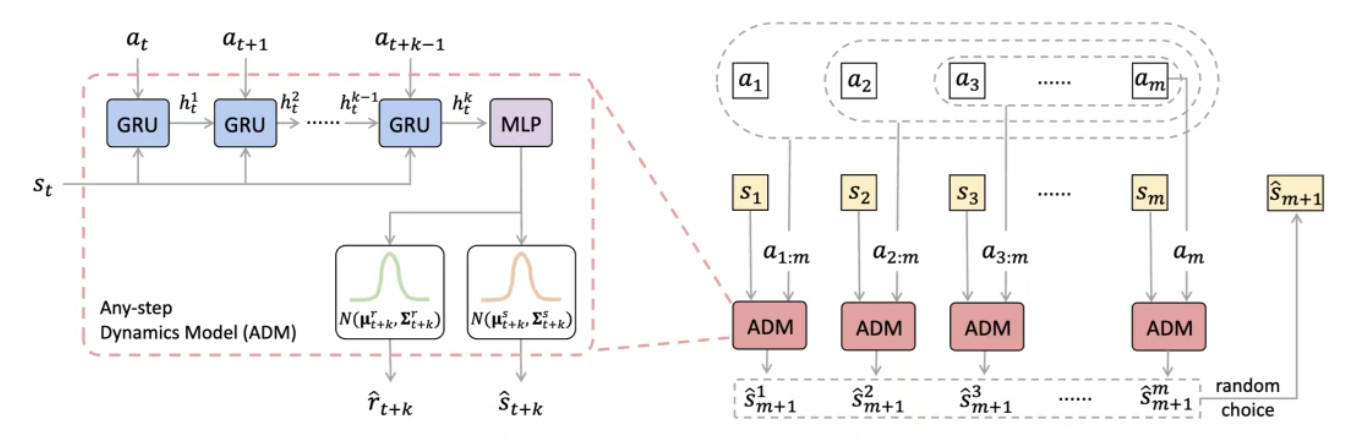
\includegraphics{images/image-0050.png}
\caption{ADM 任意步动力学模型示意图}
\end{figure}

\hypertarget{ux4e8cux6a21ux578bux67b6ux6784-3}{%
\subsubsection{（二）模型架构}\label{ux4e8cux6a21ux578bux67b6ux6784-3}}

\begin{itemize}
\tightlist
\item
  由于输入计划的步长 \(k\) 是可变的，作者采用了包含门控循环单元（GRU）的循环神经网络（RNN）来实现 ADM。
\item
  为了处理输入维度，模型会将初始的单步状态 \(s_t\) 进行复制，使其与多步动作序列的长度相匹配，然后依次送入 RNN。
\item
  RNN 输出的隐藏状态 \(h_k\) 会被送入多层感知机（MLP），最终输出目标状态 \(s_{t+k}\) 和奖励 \(r_{t+k}\) 的高斯分布参数，即均值和标准差 \((\mu_{t+k}^{s}, \Sigma_{t+k}^{s})\) 与 \((\mu_{t+k}^{r}, \Sigma_{t+k}^{r})\)。
\end{itemize}

\hypertarget{ux4e09ux8badux7ec3ux76eeux6807}{%
\subsubsection{（三）训练目标}\label{ux4e09ux8badux7ec3ux76eeux6807}}

最大化 \(k\) 步预测（\(k\) 为 \(1\) 至 \(m\) 间的任意值）的对数似然：

\[
J_T(\theta)
=
\frac{1}{m}
\sum_{k=1}^{m}
\mathbb{E}_{(s_t,a_{t:t+k-1},r_{t+k},s_{t+k}) \sim D_{\mathrm{env}}}
\left[
\log T_{\theta}^{k}(s_{t+k}, r_{t+k} \mid s_t, a_{t:t+k-1})
\right]
\]

\hypertarget{ux56dboff-policyux65f6ux7684ux4e0dux786eux5b9aux6027ux91cfux5316}{%
\subsubsection{（四）Off-policy时的不确定性量化}\label{ux56dboff-policyux65f6ux7684ux4e0dux786eux5b9aux6027ux91cfux5316}}

\begin{itemize}
\tightlist
\item
  \textbf{不确定性量化原理}：当面临轨迹分布发生变化或进入风险区域时，使用不同回溯长度 \(k\) 预测出的状态会表现出明显的分歧。ADMPO-OFF 创造性地利用这一特性，通过计算不同回溯长度 \(k\) 预测结果的方差（或标准差）来量化模型的不确定性 \(U^{\mathrm{ADM}}\)，彻底摆脱了对集成模型的依赖。
\item
  \textbf{不确定性公式}：
\end{itemize}

\[
U^{\mathrm{ADM}}(s_t, a_t)
=
\mathbb{E}_{\tau^m \sim I(\pi)}
\left[
\left\|
\frac{1}{m}
\sum_{k=1}^{m}
\left(
(\Sigma_{t}^{k})^{2}
+(\mu_t^{k})^{2}
\right)
-
(\bar{\mu})^{2}
\right\|_1
\right]
\]

\begin{itemize}
\tightlist
\item
  \textbf{悲观价值迭代机制}：在离线训练好的 ADM 中进行环境展开时，算法会对每一步生成的奖励进行惩罚：\(\tilde{r}=r-\beta U^{ADM}(s_t,a_t)\)，其中 \(\beta\) 是惩罚系数。通过惩罚高不确定性区域的奖励，算法构造了一个悲观的贝尔曼算子，强制策略保持保守，避免采取未知区域的危险动作。
\end{itemize}

\hypertarget{ux4e09adm-v2ux7684ux6539ux8fdb}{%
\subsection{三、ADM-v2的改进}\label{ux4e09adm-v2ux7684ux6539ux8fdb}}

\hypertarget{ux4e00ux72b6ux6001ux521dux59cbux5316ux4e0eux52a8ux4f5cux6f14ux5316ux5206ux79bb}{%
\subsubsection{（一）状态初始化与动作演化分离}\label{ux4e00ux72b6ux6001ux521dux59cbux5316ux4e0eux52a8ux4f5cux6f14ux5316ux5206ux79bb}}

第一代ADM通过直接建模任意步长的状态转移，减少了自举带来的误差累积。但由于其结构设计问题，ADM需要将初始状态多次复制，反复引入起始状态以对齐动作序列的长度，这导致了RNN隐藏表示与初始状态的强耦合，且无法通过并行计算加速任意步长的预测。

ADM-v2对这一结构做了更自然的重构：把状态编码和动力学预测分开，先将起始状态编码为隐变量，将这一隐表示作为循环单元的初始隐藏状态，后续递推只输入动作序列，不再重复输入起始状态。这样能让预测效果更优，也更符合基于隐变量的世界模型的范式。

\begin{figure}[htbp]
\centering
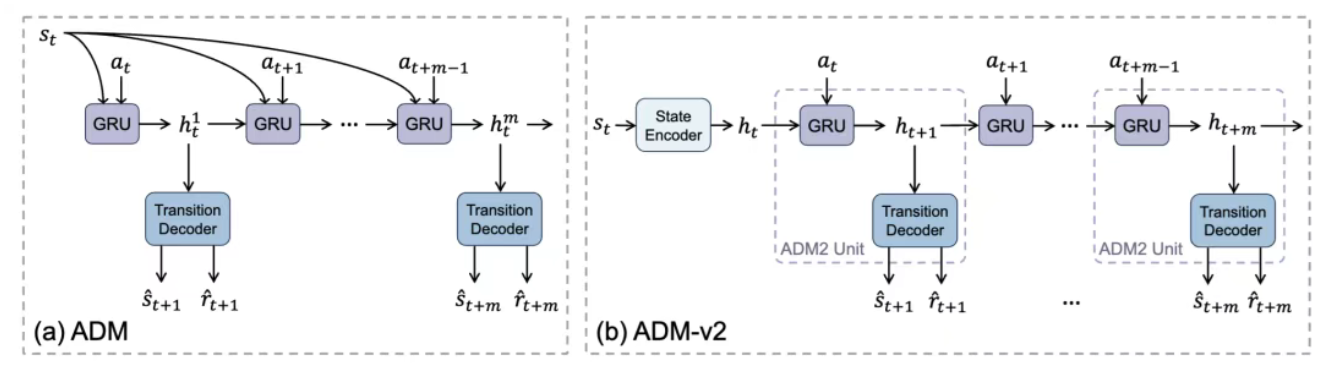
\includegraphics{images/image-0051.png}
\caption{ADM 与 ADM-v2 架构对比}
\end{figure}

模型分为三个组件：

\begin{itemize}
\tightlist
\item
  \textbf{状态编码器（State Encoder）}：将回溯起点状态 \(s_t\) 编码为隐向量 \(h_t\)，即 \(h_t=enc_{\theta}(s_t)\)。这个 \(h_t\) 直接作为 GRU 的初始隐藏状态。
\item
  \textbf{GRU 单元}：因为起点状态的信息已经压缩在 \(h_t\) 中，后续 GRU 的每次循环前向传播不再重复输入起点状态，而仅接收动作序列中的当前动作 \(a_t\)：
\end{itemize}

\[
h_{t+1}=g_{\theta}(h_t,a_t)
\]

\begin{itemize}
\tightlist
\item
  \textbf{转移解码器（Transition Decoder）}：接收更新后的隐藏状态 \(h_{t+1}\)，解码并输出下一状态 \(s_{t+1}\) 和奖励 \(r_{t+1}\) 的独立高斯分布参数：
\end{itemize}

\[
(\mu_{t+1}^{s}, \Sigma_{t+1}^{s}, \mu_{t+1}^{r}, \Sigma_{t+1}^{r})
=
\mathrm{dec}_{\theta}(h_{t+1})
\]

\hypertarget{ux4e8cux5e76ux884cux4efbux610fux6b65ux6edaux52a8ux63a8ux6f14parallel-any-step-roll-outparoll}{%
\subsubsection{（二）并行任意步滚动推演（Parallel Any-step Roll-out，PARoll）}\label{ux4e8cux5e76ux884cux4efbux610fux6b65ux6edaux52a8ux63a8ux6f14parallel-any-step-roll-outparoll}}

\begin{figure}[htbp]
\centering
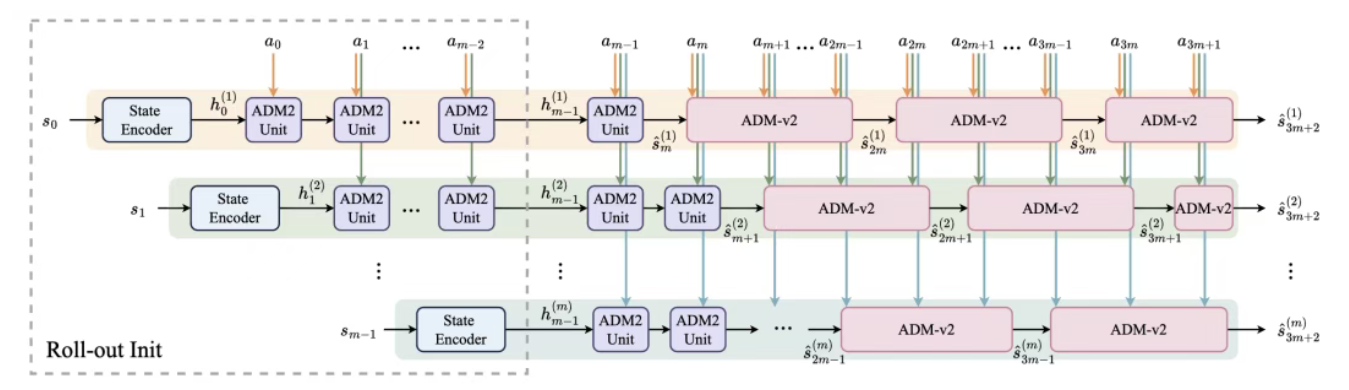
\includegraphics{images/image-0052.png}
\caption{PARoll 并行任意步滚动推演初始化示意图}
\end{figure}

如图，维护 \(m\) 个并行预测分支，每两个分支之间有 \(1\) 步的时间差，每个分支在中间都每隔 \(m\) 步（设定的最大预测步长）进行一次预测。

\textbf{第一步：轨迹初始化}

在进行模型 rollout 之前，算法首先需要构建 \(m\) 条并行的预测时间线（Timeline），其中 \(m\) 是模型训练时设定的最大预测跨度。

\begin{enumerate}
\def\labelenumi{\arabic{enumi}.}
\tightlist
\item
  \textbf{数据采样}：从真实环境离线数据集 \(D_{\mathrm{env}}\) 中采样一段长度为 \(m-1\) 的真实状态-动作序列：
\end{enumerate}

\[
(s_0,a_0,s_1,a_1,\ldots,s_{m-2},a_{m-2},s_{m-1})
\]

\begin{enumerate}
\def\labelenumi{\arabic{enumi}.}
\setcounter{enumi}{1}
\tightlist
\item
  \textbf{并行编码与对齐}：这 \(m\) 个真实状态分别作为 \(m\) 条时间线的起点。

  \begin{itemize}
  \tightlist
  \item
    第 \(1\) 条时间线以 \(s_0\) 为起点，先用状态编码器将 \(s_0\) 编码为初始隐状态 \(h_0^{(1)}\)。接着，将动作序列 \((a_0,a_1,\ldots,a_{m-2})\) 依次输入到 ADM2 Unit 中进行递归前向传播，使其时间步对齐到 \(m-1\)，最终得到隐状态 \(h_{m-1}^{(1)}\)。
  \item
    第 \(2\) 条时间线以 \(s_1\) 为起点，状态编码器将 \(s_1\) 编码为 \(h_1^{(2)}\)，然后依次输入动作 \((a_1,\ldots,a_{m-2})\) 更新隐状态，对齐到时间步 \(m-1\)，得到隐状态 \(h_{m-1}^{(2)}\)。
  \item
    依此类推，第 \(m\) 条时间线直接以 \(s_{m-1}\) 为起点，通过状态编码器编码后，直接得到时间步 \(m-1\) 的隐状态 \(h_{m-1}^{(m)}\)，无需输入任何历史动作。
  \end{itemize}
\item
  \textbf{初始化完成}：经过上述过程，我们在时间步 \(m-1\) 获得了 \(m\) 个多样化的、包含了不同历史回溯信息的隐状态集合：
\end{enumerate}

\[
(h_{m-1}^{(1)},h_{m-1}^{(2)},\ldots,h_{m-1}^{(m)})
\]

\textbf{第二步：并行生成 Roll-out 与多样化预测}

从时间步 \(t=m-1\) 开始，模型正式进入未知未来的 rollout 阶段。

\begin{enumerate}
\def\labelenumi{\arabic{enumi}.}
\tightlist
\item
  \textbf{动作采样与隐状态并行更新}：策略网络 \(\pi\) 根据当前状态给出动作 \(a_{m-1}\)。此时，\(m\) 条时间线上的 ADM2 Unit 并行接收这个动作，并同步更新各自的隐状态：
\end{enumerate}

\[
h_m^{(i)}=g_\theta(h_{m-1}^{(i)},a_{m-1})
\]

其中 \(i\in\{1,2,\ldots,m\}\) 代表不同的时间线。

\begin{enumerate}
\def\labelenumi{\arabic{enumi}.}
\setcounter{enumi}{1}
\tightlist
\item
  \textbf{状态与奖励的并行解码}：接着，转移解码器并行对这 \(m\) 个隐状态进行解码，输出预测状态和奖励的高斯分布参数，并从中采样：
\end{enumerate}

\[
(\mu_{s_m}^{(i)},\Sigma_{s_m}^{(i)},\mu_{r_m}^{(i)},\Sigma_{r_m}^{(i)})
=
dec_\theta(h_m^{(i)})
\]

\[
\hat{s}_m^{(i)}\sim\mathcal{N}(\mu_{s_m}^{(i)},\Sigma_{s_m}^{(i)}),
\quad
\hat{r}_m^{(i)}\sim\mathcal{N}(\mu_{r_m}^{(i)},\Sigma_{r_m}^{(i)})
\]

\begin{enumerate}
\def\labelenumi{\arabic{enumi}.}
\setcounter{enumi}{2}
\item
  \textbf{预测多样性的来源}：在同一时间步 \(m\) 预测出的 \(m\) 个状态 \((\hat{s}_m^{(1)},\hat{s}_m^{(2)},\ldots,\hat{s}_m^{(m)})\) 具有天然的多样性，因为它们来自不同的回溯起点和不同长度的跨度（Stride）直接预测而来。例如，\(\hat{s}_m^{(1)}\) 是从 \(s_0\) 经过 \(m\) 步动作演化而来，而 \(\hat{s}_m^{(m)}\) 是从 \(s_{m-1}\) 经过 \(1\) 步动作演化而来。
\item
  \textbf{持续演化}：对于后续的时间步 \(t\gt m\)，算法重复执行并行的隐状态更新和解码生成操作。在此过程中，从 \(m\) 个多样化预测中均匀随机选择一个作为下一步策略采样的依据，并同时利用这些预测的方差来并行估计当前步的模型不确定性 \(U^{ADM2}\)。
\end{enumerate}

\textbf{模型不确定性估计}：在每一步 \(t\)，算法从上述 \(m\) 个多样化预测中均匀选取一个作为下一步的真实采样，并利用不同时间线的分布方差来量化模型在该处的不确定性（Model Uncertainty, \(U^{ADM2}\)）：

\[
U^{\mathrm{ADM2}}(s_t,a_t)
=
\mathbb{E}
\left[
\left\|
\frac{1}{m}
\sum_{k=1}^{m}
\left(
(\Sigma_{s_t}^{(k)})^2
+
(\mu_{s_t}^{(k)})^2
\right)
-
(\bar{\mu}_t)^2
\right\|_1
\right]
\]

\textbf{第三步：跨度重置}

由于 ADM-v2 在训练时设定了最大预测跨度为 \(m\)，多步直接预测（即隐状态的连续传播）不能无限期地进行下去，否则会导致严重的误差累积。

\begin{enumerate}
\def\labelenumi{\arabic{enumi}.}
\item
  \textbf{重置触发条件}：当某条时间线的直接预测步数达到最大跨度 \(m\) 时，必须截断隐状态的传播，并进行重置（Reset）。
\item
  \textbf{重置方法}：调用状态编码器（State Encoder），将该时间线在当前时间节点刚刚预测出的状态重新编码，作为新的起始隐状态送入下一个长度为 \(m\) 的预测窗口。例如，对于第 \(i\) 条时间线，它的重置时间节点是 \((m+i-1,2m+i-1,3m+i-1,\ldots)\)，此时隐状态更新方式变为：
\end{enumerate}

\[
h_{m+i-1}^{(i)}=\mathrm{enc}_\theta(\hat{s}_{m+i-1}^{(i)})
\]

\begin{enumerate}
\def\labelenumi{\arabic{enumi}.}
\setcounter{enumi}{2}
\tightlist
\item
  \textbf{交错重置的高效性}：在图中可以清晰地看到，不同时间线的重置操作（图中右侧断开的箭头并重新引入 ADM-v2 块的起点）在时间轴上是交错排列的（呈对角线状）。在实际执行时，每个时间步仅有一条时间线（具体为 \((t\bmod m)+2\)）会达到最大跨度并触发重置。这意味着每一步只需要执行一次额外的状态编码器前向传播，极大地保证了算法的运行效率。
\end{enumerate}

这意味着每隔 \(m\) 步就要把隐状态输出为预测状态，以此重新编码新的隐状态，完成重置。这样相比于随机回溯步数的好处在于，无论随机选中哪一条分支，都能获得来自历史较远状态和较近状态的信息（每隔 \(m\) 步一个状态），更好地满足平衡防止误差累积和提高精度的需要。

\hypertarget{ux56dbux5168ux89c6ux91cerolloutux7684ux7406ux8bbaux8fb9ux754c}{%
\subsubsection{（四）全视野rollout的理论边界}\label{ux56dbux5168ux89c6ux91cerolloutux7684ux7406ux8bbaux8fb9ux754c}}

\begin{enumerate}
\def\labelenumi{\arabic{enumi}.}
\tightlist
\item
  \textbf{离线策略优化：ADM2PO-fh}
\end{enumerate}

在离线学习中，策略极易陷入动力学模型预测不准确（即不确定性高）的未来系数区域（Out-of-distribution）。ADM-v2 利用 PARoll 估计的不确定性 \(U^{ADM2}\) 作为悲观惩罚项（Penalty term）。

\begin{itemize}
\tightlist
\item
  \textbf{定理 3.1（不确定性量化器有效性）}：论文证明了 \(\beta\cdot U^{\mathrm{ADM2}}\) 是一个合法的 \(\epsilon\)-不确定性量化器。它严格界定了真实 Bellman 算子与 ADM-v2 代理算子之间的误差上界：
\end{itemize}

\[
\left|
\hat{T}^{\pi}Q(s_t,a_t)
-
T^{\pi}Q(s_t,a_t)
\right|
\le
\beta\cdot U^{\mathrm{ADM2}}(s_t,a_t)
\]

\begin{itemize}
\tightlist
\item
  \textbf{应用}：基于此，ADM2PO-fh 算法在 \(Q\) 值估计中引入修正项：
\end{itemize}

\[
\hat{T}^{\mathrm{ADM2}}Q(s_t,a_t)
:=
\hat{T}^{\pi}Q(s_t,a_t)
-
\beta\cdot U^{\mathrm{ADM2}}(s_t,a_t)
\]

从而在面临高风险区域时收紧 \(Q\) 值，防止过估计。

\begin{enumerate}
\def\labelenumi{\arabic{enumi}.}
\setcounter{enumi}{1}
\tightlist
\item
  \textbf{离线策略评估（OPE）：ADM2OPE}
\end{enumerate}

ADM-v2 可以直接作为一个 surrogate environment（代理环境），通过让待评估的策略在模型中进行 \(N\) 次完整的全视野轨迹采样，取平均回报作为策略的评估值。

\begin{itemize}
\tightlist
\item
  \textbf{定理 3.2（性能边界 Bounds）}：评估回报与真实回报的差距受限于长期预测误差和策略散度。论文证明了返回的差距受到 \(C(\delta_{\max},\epsilon_r)\) 的约束：
\end{itemize}

\[
\left|
\eta(\pi)-\hat{\eta}(\pi)
\right|
\le
\frac{2\gamma r_{\max}\delta_{\max}}{(1-\gamma)(1-\gamma^m)}
+
\frac{2\gamma r_{\max}\epsilon_\pi}{(1-\gamma)^2}
+
\frac{4r_{\max}\epsilon_r}{1-\gamma}
\]

\begin{itemize}
\tightlist
\item
  \textbf{核心结论}：当最大 \(m\) 步直接预测误差满足特定条件（\(\delta_{\max}\lt\frac{\delta(1-\gamma^m)}{1-\gamma}\)）时，ADM-v2 生成的 OPE 误差上界比传统的单步动力学模型更加紧致（Tighter），理论上提供了更可靠的评估。
\end{itemize}

\hypertarget{ux53c2ux8003ux6587ux732e-190}{%
\subsection{参考文献}\label{ux53c2ux8003ux6587ux732e-190}}

\begin{itemize}
\tightlist
\item
  Lin, H., Xu, Y.-Y., Sun, Y., Zhang, Z., Li, Y.-C., Jia, C., Ye, J., Zhang, J., \& Yu, Y. (2025). \href{https://openreview.net/forum?id=JZCxlrwjZ8}{Any-step Dynamics Model Improves Future Predictions for Online and Offline Reinforcement Learning}. ICLR.
\item
  Lin, H., Xiao, S., Li, Y.-C., Zhang, Z., Sun, Y., Jia, C., \& Yu, Y. (2026). \href{https://openreview.net/forum?id=ICbXEwqpga}{ADM-v2: Pursuing Full-Horizon Roll-out in Dynamics Models for Offline Policy Learning and Evaluation}. ICLR.
\end{itemize}

\clearpage

\hypertarget{action-spaceux7684ux5b66ux4e60ux8bbaux6587}{%
\section{Action Space的学习（论文）}\label{action-spaceux7684ux5b66ux4e60ux8bbaux6587}}

\begin{quote}
本文是论文阅读笔记，内容代表对应论文方法或作者理解，不应直接视为领域共识或工程最佳实践。
\end{quote}

\hypertarget{ux4e00latent-action-models}{%
\subsection{一、Latent Action Models}\label{ux4e00latent-action-models}}

世界模型的核心表达式是 \(s_{t+1}=f(s_t,a_t)\)。对于海量的视频数据，\(s_t\) 和 \(s_{t+1}\) 都是容易获取的，但我们却没有显式的动作数据 \(a_t\)。这会影响模型学习``特定干预会造成何种后果''，尤其是在交互式或具身智能场景中更明显。如果将动作看作一种模态，那么模型也需要一个对应的``词表''，即 Action Space。Latent Action Models 是一种从视频中自监督学习 Action Space 的方法。

\hypertarget{ux4e00ux6838ux5fc3ux7ec4ux4ef6}{%
\subsubsection{（一）核心组件}\label{ux4e00ux6838ux5fc3ux7ec4ux4ef6}}

\begin{enumerate}
\def\labelenumi{\arabic{enumi}.}
\tightlist
\item
  反向动力学模型（Inverse Dynamics Model）：从前后状态 \(s_t\) 和 \(s_{t+1}\) 中推断动作 \(a_t\) 的潜在表示，并通过信息瓶颈促使 \(a_t\) 编码最关键的运动信息。
\item
  前向动力学模型（Forward Dynamics Model）：使用当前状态 \(s_t\) 和动作 \(a_t\) 预测下一状态 \(s_{t+1}\)。
\end{enumerate}

\hypertarget{ux4e8cux62bdux8c61ux8981ux6c42}{%
\subsubsection{（二）抽象要求}\label{ux4e8cux62bdux8c61ux8981ux6c42}}

如果允许动作 \(a_t\) 保留太多信息以提升生成质量，它又容易混入颜色、纹理、背景等内容信息，导致动作不够抽象、难以迁移。为了保证动作表示具有可迁移性和抽象性，模型通常会施加强预测瓶颈，例如向量量化或变分瓶颈。

但不可否认的是，如果动作表示被压缩得足够抽象，它更容易迁移，却也可能偏离动作空间内在的流形结构，丢失预测下一个状态的准确性，以及生成所需的细节。

\hypertarget{ux4e8cux52a8ux4f5cux62bdux8c61ux5316ux4e2dux7684ux7ed3ux6784-ux5185ux5bb9ux8868ux5f81ux89e3ux8026ux65b9ux6cd5}{%
\subsection{二、动作抽象化中的结构-内容表征解耦方法}\label{ux4e8cux52a8ux4f5cux62bdux8c61ux5316ux4e2dux7684ux7ed3ux6784-ux5185ux5bb9ux8868ux5f81ux89e3ux8026ux65b9ux6cd5}}

\hypertarget{ux4e00ux6838ux5fc3ux601dux60f3-25}{%
\subsubsection{（一）核心思想}\label{ux4e00ux6838ux5fc3ux601dux60f3-25}}

前面提到，对于 Latent Action Models 提取动作，一方面需要施加信息瓶颈以保证动作的抽象性；另一方面，如果压缩过度又会影响预测准确性。对于这一对矛盾，论文《DiLA: Disentangled Latent Action World Models》提出了结构-内容解耦的方法：将时空变换结构与视觉内容的表征解耦，在动作（即状态随时空变换的结构）上采取严格的信息瓶颈，在视觉内容方面则通过额外通道避免信息丢失。

\hypertarget{ux4e8cux6a21ux578bux67b6ux6784ux4e0eux5de5ux4f5cux6d41-1}{%
\subsubsection{（二）模型架构与工作流}\label{ux4e8cux6a21ux578bux67b6ux6784ux4e0eux5de5ux4f5cux6d41-1}}

输入视频先经过 DINOv2 编码器和 Spatial-Temporal Transformer，得到视觉表征。随后，模型将这些表征分别送入不同通路中处理：

\begin{enumerate}
\def\labelenumi{\arabic{enumi}.}
\tightlist
\item
  结构通路：负责建模与运动相关的空间结构，例如位置、布局和动态变化。模型先压缩得到结构表征，再用逆向动力学模型从连续结构表征的差异中推断动作的潜在表示。前向动力学模型根据当前结构表征和动作预测下一时刻的结构表征。这个过程使动作表征主要编码``结构如何变化''，而不是完整图像如何变化。
\item
  内容通路：负责保存视觉细节，例如颜色、纹理、背景、物体外观和历史信息。模型使用线性注意力 Mamba 层作为记忆模块，用于聚合历史内容信息。它关注相对稳定的视觉内容，而不是快速变化的动态结构。
\end{enumerate}

最后，Fusion Decoder 将预测出的结构表征、内容记忆表征以及初始帧信息融合起来，重建未来视觉表征。

\begin{figure}[htbp]
\centering
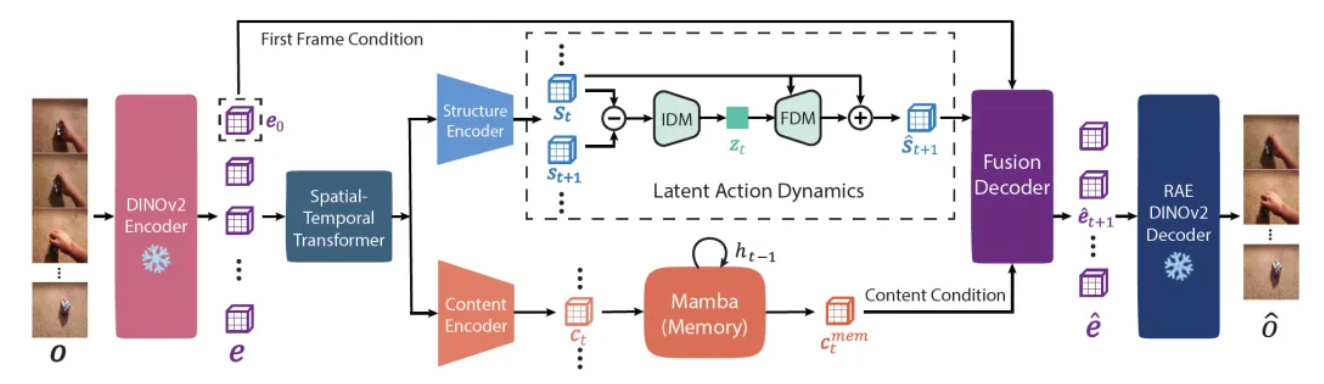
\includegraphics{images/image-0053.png}
\caption{DiLA 动作空间学习模型架构}
\end{figure}

为了验证结构与内容是否真正分离，论文设计了实验：从一个视频中提取结构，从另一个视频中提取内容，然后将二者重新组合生成新序列。生成序列继承了结构序列的空间动态，同时保留了内容序列的颜色、纹理和外观属性。而固定结构表征，只让内容的记忆模块随时间更新，序列保持静止。这说明内容记忆模块主要编码时间上相对稳定的内容信息，而不是运动本身。

\hypertarget{ux53c2ux8003ux6587ux732e-191}{%
\subsection{参考文献}\label{ux53c2ux8003ux6587ux732e-191}}

\begin{itemize}
\tightlist
\item
  Schmidt, D., \& Jiang, M. (2024). \href{https://openreview.net/forum?id=rnnt2Be6nN}{Learning to Act without Actions}. International Conference on Learning Representations.
\item
  Garrido, Q., Nagarajan, T., Terver, B., Ballas, N., LeCun, Y., \& Rabbat, M. (2026). \href{https://arxiv.org/abs/2601.05230}{Learning Latent Action World Models In The Wild}. arXiv:2601.05230.
\end{itemize}

\clearpage


% 在抽象表示空间中预测的世界模型
\hypertarget{ux5728ux62bdux8c61ux8868ux793aux7a7aux95f4ux4e2dux9884ux6d4bux7684ux4e16ux754cux6a21ux578b}{%
\chapter{在抽象表示空间中预测的世界模型}\label{ux5728ux62bdux8c61ux8868ux793aux7a7aux95f4ux4e2dux9884ux6d4bux7684ux4e16ux754cux6a21ux578b}}

\hypertarget{v-jepaux8bbaux6587}{%
\section{V-JEPA（论文）}\label{v-jepaux8bbaux6587}}

\begin{quote}
本文是论文阅读笔记，内容代表对应论文方法或作者理解，不应直接视为领域共识或工程最佳实践。
\end{quote}

\hypertarget{ux4e00ux6838ux5fc3ux601dux60f3-26}{%
\subsection{一、核心思想}\label{ux4e00ux6838ux5fc3ux601dux60f3-26}}

在 V-JEPA 之前，主流的视频无监督学习通常依赖于像素级重建（Pixel Reconstruction），例如掩码自编码器 VideoMAE。然而，在像素空间进行预测存在明显劣势：模型必须分配大量计算能力和模型容量来捕捉视觉输入中那些低层次、甚至是无关紧要的细节。

V-JEPA 的核心思想是特征空间预测（Feature Prediction）：

\begin{itemize}
\tightlist
\item
  该模型完全摒弃了像素重建，不再预测原始像素，而是预测被遮挡区域在语义特征空间中的表示。
\item
  通过在隐性表示空间（Latent Space）中进行预测，模型能够灵活地消除视频中不可预测或与语义无关的像素级细节，从而学习到高度通用的视觉特征。
\end{itemize}

其他基于隐变量的方法更像Decoder，按时序生成下一时刻的隐变量；V-JEPA更像Encoder，在时空上进行掩码预测，且没有重建损失（即由隐变量生成画面或间接参与生成画面）。

\hypertarget{ux4e8cux6838ux5fc3ux67b6ux6784ux4e0eux635fux5931ux51fdux6570}{%
\subsection{二、核心架构与损失函数}\label{ux4e8cux6838ux5fc3ux67b6ux6784ux4e0eux635fux5931ux51fdux6570}}

V-JEPA 的核心架构由三个部分组成：编码器 \(E_\theta(\cdot)\)、预测器 \(P_\theta(\cdot)\) 以及目标编码器 \(E_{\theta'}(\cdot)\)。目标是让从视频某一部分 \(x\) 计算出的表示，能够预测视频另一部分 \(y\) 的表示。

为了防止模型输出常数向量从而陷入``表示坍塌''（Representation Collapse），V-JEPA 借鉴了非对比学习策略，采用了带有停止梯度（Stop-gradient）的指数移动平均（EMA）架构。

模型的优化目标是最小化预测特征与目标特征之间的 \(L_1\) 距离：

\[
\begin{aligned}
\mathcal{L}_{\mathrm{VJEPA}}
&=
\left\|
P_\theta(E_\theta(x),\Delta_y)
\, - \, \mathrm{sg}(E_{\theta'}(y))
\right\|_1
\end{aligned}
\]

其中，\(\mathrm{sg}(\cdot)\) 表示停止梯度操作，\(E_{\theta'}(\cdot)\) 是 \(E_\theta(\cdot)\) 权重的指数移动平均网络，\(\Delta_y\) 是提供给预测器的位置条件变量。

解释：

\begin{enumerate}
\def\labelenumi{\arabic{enumi}.}
\item
  用 \(L_1\) 范数是因为受极端值影响小，实验发现更稳定。其仅在 \(0\) 处不可导（类似 ReLU）。
\item
  由于没有重建损失，为了防止``模式崩塌''，\(y\) 的 encoder 更新方法类似于强化学习的``目标网络''，即从 \(x\) 的 encoder 网络软更新：
\end{enumerate}

EMA 更新（\(y\)-encoder）：\(y\)-encoder 的权重 \(\theta'_t\) 不使用优化器更新，而是使用指数移动平均公式缓慢更新：

\[
\theta'_t=\tau\theta'_{t-1}+(1-\tau)\theta_t
\]

其中 \(\tau\) 是动量参数，在 V-JEPA 中从 \(0.998\) 逐渐增加到 \(1.0\)。也就是说，\(y\)-encoder 始终是 \(x\)-encoder 历史状态的一个平滑、滞后的影子。

为什么这样能防止模式崩塌：

假设我们固定住编码器，只训练预测器 \(P_\theta\)。模型的损失函数是 \(L_1\) 范数（绝对误差）。在统计学中，使得绝对误差期望最小的预测值，正是目标分布的中位数。

当预测器已经训练得非常完美（即 \(P=P^{*}\)）时，我们将它代回损失函数，这时候整个损失函数就变成了计算目标 \(Y\) 的条件中位绝对偏差（Median Absolute Deviation，简称 MAD）：

\[
\begin{aligned}
\mathrm{MAD}(Y\mid E_\theta(x))
&=
\mathbb{E}
\left[
\left|
Y-\mathrm{median}(Y\mid E_\theta(x))
\right|
\right]
\end{aligned}
\]

此时，编码器 \(E_\theta\) 的优化方向（梯度）就是去最小化这个 MAD。

直观解释：

\begin{itemize}
\tightlist
\item
  如果 \(E_\theta(x)\) 抽取了``什么都没学到、输出常数''，那么它就无法提供关于目标 \(Y\) 的任何线索。此时 \(Y\) 在给定 \(E_\theta(x)\) 条件下的分布会非常分散，其 MAD 值会非常大。
\item
  为了最小化 MAD，编码器 \(E_\theta(x)\) 必须从输入视频中抽取有效信息，使得它能够高度确定地推出 \(Y\) 的状态。当 \(E_\theta(x)\) 包含的信息越丰富，目标 \(Y\) 的不确定性就越小，分布越集中，MAD 也越小。
\item
  虽然最小化 MAD 能促使编码器学习，但如果目标 \(Y\)（由 \(y\)-encoder 生成）和预测器更新得一样快，它们可能会``合谋''一起变成常数来让 MAD 变为 \(0\)。
\item
  这就是 EMA 的原因：\(y\)-encoder 的权重不是通过梯度下降更新的，而是 \(x\)-encoder 权重的历史平均版本。这使得 \(y\)-encoder 的变化非常缓慢。
\end{itemize}

工作流：

\begin{enumerate}
\def\labelenumi{\arabic{enumi}.}
\tightlist
\item
  预测器学得很快，迅速逼近最优解 \(P^{*}\)。
\item
  因为目标 \(Y\) 变化很慢，它不会配合 \(x\)-encoder 一起坍塌。
\item
  迫于快速进化的预测器和稳定缓慢的目标，\(x\)-encoder 只能老老实实地去学习如何提取丰富的信息来降低 MAD，从而从根本上切断了坍塌的可能。
\end{enumerate}

这意味着通过软更新的方式把在线网络的参数复制给目标网络，可以让目标网络的变化总是落后于 \(E_\theta(x)\)，且目标网络只能被动随着在线网络变化而变化，就像在线网络在追一个``移动的靶子''，避免了双方共同奔向常数的捷径。

\hypertarget{ux4e09ux8badux7ec3ux65b9ux6cd5-1}{%
\subsection{三、训练方法}\label{ux4e09ux8badux7ec3ux65b9ux6cd5-1}}

\hypertarget{ux4e00ux63a9ux7801tokenux9884ux6d4b}{%
\subsubsection{（一）掩码token预测}\label{ux4e00ux63a9ux7801tokenux9884ux6d4b}}

\begin{itemize}
\item
  模型首先从视频中抽取一个包含 \(16\) 帧的短视频片段（时间步幅为 \(4\)），并将其空间分辨率调整为 \(224\times224\)，张量形状为 \(16\times224\times224\times3\)。
\item
  使用 3D 卷积层（过滤器大小 \(2\times16\times16\)）对视频进行切块，将其展平为一维的词元（Token）序列，序列长度为 \(1568\)。
\item
  将绝对 3D 正弦-余弦位置嵌入（Position Embeddings）添加到该特征图中。
\item
  采用多块采样策略：提取短程掩码（覆盖 \(15\%\) 面积的 \(8\) 个随机块）和长程掩码（覆盖 \(70\%\) 面积的 \(2\) 个随机块）。平均掩码比例高达约 \(90\%\)。
\item
  构建一组可学习的``掩码 Token''，这些 Token 包含了缺失区域的三维时空位置信息。
\item
  预测器网络（一个较窄的 Transformer）接收上下文表示和掩码 Token，并在隐空间中直接输出对缺失区域特征的预测值 \(\hat{s}_y\)。
\item
  在预测特征 \(\hat{s}_y\) 和真实特征 \(s_y\) 之间计算 \(L_1\) 距离损失。
  为什么不严格按时序因果：
\end{itemize}

\begin{enumerate}
\def\labelenumi{\arabic{enumi}.}
\tightlist
\item
  \textbf{物理世界的非严格因果性}：在视觉世界中，我们不仅可以通过``过去''预测``未来''，也可以通过``未来''和``周围环境''推断``过去''或``被遮挡的部分''。V-JEPA 的多块掩码策略（Multi-Block Masking）会在时空中随机挖掉一大块（高达 \(90\%\)），模型必须学会利用空间上下文和时间前后的线索来填补隐空间中的空白。
\item
  \textbf{因果掩码的消融实验结果}：论文做过对比实验。他们尝试了一种``因果掩码''（Causal Multi-block）策略：只给模型看视频前几帧，让它预测后面几帧。结果发现，这种严格遵循因果律的训练方式，其下游任务表现反而下降了。
\item
  \textbf{结论}：V-JEPA 的目标是提取通用的视觉表示（Motion and Appearance），而不是像视频生成模型那样生成符合因果约束的下一帧图像。随机的时空掩码会强迫模型学习到比纯因果预测更稳健的物理规律，例如物体的空间一致性、运动的连续性。
\end{enumerate}

\hypertarget{ux4e8cux975eux63a9ux7801tokenux7684ux635fux5931ux51fdux6570}{%
\subsubsection{（二）非掩码token的损失函数}\label{ux4e8cux975eux63a9ux7801tokenux7684ux635fux5931ux51fdux6570}}

在V-JEPA 2.1中，为了更充分地利用数据以及让模型更好地理解连续性，对非掩码token也引入了损失，要求预测这些未被遮挡的特征：

但这里存在一个致命的逻辑漏洞：对于可见的上下文块，模型其实已经``看到了''它的输入特征。如果直接要求模型去预测这些可见块，网络很容易找到一个``捷径''（Trivial Solution）：直接把输入特征原封不动地复制（Copy）到输出端。一旦模型开始``抄作业''，它就不会再去费力学习真正有用的空间结构和特征了。

为了解决这个问题，论文设计了动态加权公式：

\[
\lambda_i = \frac{\lambda}{\sqrt{d_{\min}(i, M)}}
\]

\begin{itemize}
\item
  \(d_{\min}(i, M)\)：表示当前可见的上下文块（Token）\(i\) 距离最近的一个被遮挡块（Masked Token）的时空距离（以块为单位）。
\item
  \(\sqrt{d_{\min}(i, M)}\)：对这个距离开平方根，作为分母。
\item
  \textbf{整体逻辑}：距离掩码区域越近的可见块，其计算损失时的权重 \(\lambda_i\) 越大；距离掩码区域越远的可见块，权重越小。
  这样设计的好处：
\item
  \textbf{强制学习局部连续性（Local Continuity）}：通过给靠近遮挡边缘的可见块赋予更高权重，模型被强迫去关注可见区域与被遮挡区域是如何在空间和时间上平滑过渡的。它不能再简单地``复制''自己的特征，而是必须结合邻居的状态来推断。
\item
  \textbf{平衡``全局理解''与``局部细节''}：如果所有可见块权重一样大（哪怕是一个固定的很小的值），都会导致模型在动作识别（如 SSv2 数据集）等全局语义任务上性能大幅下降。这种动态距离衰减机制，既让模型学会了精细的边界分割（Segmentation），又保住了动作识别等全局任务的能力，实现了一个绝佳的平衡（Trade-off）。
\end{itemize}

\hypertarget{ux4e09ux6df1ux5ea6ux81eaux76d1ux7763}{%
\subsubsection{（三）深度自监督}\label{ux4e09ux6df1ux5ea6ux81eaux76d1ux7763}}

在传统的视觉 Transformer（ViT）中，越靠近底层的网络层提取的是边缘、纹理等``局部细节''，越靠近顶层的网络层提取的是物体类别、动作意图等``全局概念''。这通常会导致顶层特征在经历层层传递后，丢失大量细粒度的空间信息。

V-JEPA 2.1 的深度自监督彻底改变了这一点。
1. \textbf{具体是怎么操作的？}
- \textbf{特征提取与融合}：x-编码器处理可见块时，不仅仅输出最后一层的特征，还会把其中 \(3\) 个中间层的特征提取出来，与最后一层的特征在通道维度上拼接在一起。
- \textbf{降维与输入}：拼接后的庞大特征会通过一个轻量级的多层感知机（MLP）进行降维融合，然后与代表遮挡位置的掩码标记（Mask Tokens）拼接，一起送入预测器（Predictor）。
- \textbf{分层预测与计算损失}：预测器不再只输出一个最终结果，而是同时输出 \(4\) 个层级的预测结果（对应刚才提取的 \(4\) 个编码器层级）。模型会分别把这 \(4\) 个预测结果，与目标网络（y-编码器）对应 \(4\) 个层级的输出进行对比，在每一个层级上都计算一遍预测损失和上下文损失。
2. \textbf{这样做有什么好处？}
- \textbf{通过顶层保留底层细节}：因为预测器在最终输出时不仅要预测高级语义，还要``倒推''并准确预测出网络中间层那些包含丰富空间几何信息的局部特征。这种监督信号会一直反向传播，强制局部细节信息从底层一直流向最终层。
- \textbf{下游任务使用极其方便（无需多层拼接）}：以前在做语义分割或深度估计时，为了获取足够的细节，研究人员通常需要手动把模型不同深度的层特征``拼接''起来使用。V-JEPA 2.1 经过深度自监督训练后，只用它的最后一层特征（Last-Layer），就能达到极高的密集预测性能，几乎去除了对多层融合的依赖，大大简化了下游任务的部署。
- \textbf{强势回血全局性能}：论文发现，单纯引入上下文损失会损害全局分类任务的准确率，但一旦加上深度自监督，不仅密集任务（如分割、深度）性能进一步飙升，原本流失的全局理解能力（如动作分类）也被成功挽救回来。

\hypertarget{ux56dbux4e0ellmux7684ux7ed3ux5408}{%
\subsection{四、与LLM的结合}\label{ux56dbux4e0ellmux7684ux7ed3ux5408}}

预训练完成后，我们得到了一个不懂人类语言，但对物理世界、物体外观和运动规律有着极深理解的模型。在V-JEPA 2和LLM之间加入一个投影器（Projector，通常是多层感知机MLP），把V-JEPA 2提取出的纯视觉特征（视觉Token），``翻译''并映射到大语言模型能够理解的输入空间（文本嵌入空间）中。然后用大规模的``图像/视频-文本''问答对齐数据来训练这个整体系统，就可以让其逐步学会了如何理解由V-JEPA 2传递过来的视觉信息，并能通过LLM的处理用自然语言回答关于视频内容的问题，实现初步的空间推理。

\hypertarget{ux53c2ux8003ux6587ux732e-192}{%
\subsection{参考文献}\label{ux53c2ux8003ux6587ux732e-192}}

\begin{itemize}
\tightlist
\item
  Bardes, A., Garrido, Q., Ponce, J., et al.~(2024). \href{https://arxiv.org/abs/2404.08471}{V-JEPA: Revisiting Feature Prediction for Learning Visual Representations from Video}. arXiv:2404.08471.
\item
  Assran, M., Duval, Q., Misra, I., et al.~(2023). \href{https://arxiv.org/abs/2301.08243}{Self-Supervised Learning from Images with a Joint-Embedding Predictive Architecture}. CVPR.
\end{itemize}

\clearpage

\hypertarget{ux9690ux53d8ux91cfux7684ux65f6ux95f4ux76f4ux9053ux5316ux8bbaux6587}{%
\section{隐变量的时间直道化（论文）}\label{ux9690ux53d8ux91cfux7684ux65f6ux95f4ux76f4ux9053ux5316ux8bbaux6587}}

\begin{quote}
本文是论文阅读笔记，内容代表对应论文方法或作者理解，不应直接视为领域共识或工程最佳实践。
\end{quote}

\hypertarget{ux4e00ux95eeux9898ux80ccux666f-13}{%
\subsection{一、问题背景}\label{ux4e00ux95eeux9898ux80ccux666f-13}}

传统预训练视觉编码器（如基于重构或对比学习的模型）虽然能提取丰富的语义特征，但它们并非为``规划''量身定制。这些模型生成的潜在空间轨迹（Latent Trajectories）通常是高度弯曲的。在高度弯曲的空间中进行规划时，两点之间的欧几里得距离（Euclidean distance）无法真实反映它们之间的到达难度（Geodesic distance，即实际的物理转移和动作成本）。这会导致基于梯度的规划器极易陷入局部最优，从而大幅降低决策和控制的效率。

\textbf{感知直道化假说（Perceptual Straightening Hypothesis）}：该研究的灵感来源于人类视觉神经科学中的``感知直道化''假说。研究表明，人类视觉系统在处理自然界中复杂的动态视频流时，为了更好地预测物体的运动，倾向于在内部将其转化为更平直的表征轨迹。受此启发，作者提出在人工智能的世界模型中引入``时间直道化''（Temporal Straightening），强制要求编码器学习到的潜在状态转移轨迹在局部尽可能保持直线。
\#\#\# 二、核心算法

直道化的核心是要求潜空间中的运动轨迹尽可能接近匀速直线运动。公式上，这体现为相邻两个时间步的``位移向量''应该尽可能一致：

\[
\Delta z_t = z_t - z_{t-1}
\]

\[
\Delta z_{t+1} = z_{t+1} - z_t
\]

故可以在预测下一状态的隐变量z\_t+1时，除了预测损失外，还额外引入一个基于曲率的损失函数作为正则化项。

\begin{enumerate}
\def\labelenumi{\arabic{enumi}.}
\tightlist
\item
  基于MSE Loss
\end{enumerate}

\[
\mathcal{L}_{curv} = \mathbb{E}_t\left[\left\| (z_{t+1}-z_t) - (z_t-z_{t-1}) \right\|^2\right]
\]

\begin{enumerate}
\def\labelenumi{\arabic{enumi}.}
\setcounter{enumi}{1}
\tightlist
\item
  基于余弦相似度的损失
\end{enumerate}

\[
\mathrm{Curvature}(z_{t-1}, z_t, z_{t+1}) = 1 - \frac{\Delta z_t \cdot \Delta z_{t+1}}{\|\Delta z_t\|\,\|\Delta z_{t+1}\|}
\]

\hypertarget{ux53c2ux8003ux6587ux732e-193}{%
\subsection{参考文献}\label{ux53c2ux8003ux6587ux732e-193}}

\begin{itemize}
\tightlist
\item
  Wang, Y., Bounou, O., Zhou, G., Balestriero, R., Rudner, T. G. J., LeCun, Y., \& Ren, M. (2026). \href{https://arxiv.org/abs/2603.12231}{Temporal Straightening for Latent Planning}. arXiv:2603.12231.
\end{itemize}

\clearpage

\hypertarget{leworldmodelux8bbaux6587}{%
\section{LeWorldModel（论文）}\label{leworldmodelux8bbaux6587}}

\begin{quote}
本文是论文阅读笔记，内容代表对应论文方法或作者理解，不应直接视为领域共识或工程最佳实践。
\end{quote}

\hypertarget{ux4e00ux95eeux9898ux80ccux666f-14}{%
\subsection{一、问题背景}\label{ux4e00ux95eeux9898ux80ccux666f-14}}

世界模型（World Models）旨在通过学习环境的动态演变规律，使智能体能够在``想象''中预测未来并进行规划。联合嵌入预测架构（JEPA）是近年来非常受关注的一种世界模型框架，它不直接像素空间重建图像，而是将观测数据压缩到一个紧凑的、低维的潜在空间（Latent Space）中，并在该空间内预测未来的表征。

然而，现有的端到端 JEPA 方法面临一个致命痛点：\textbf{表征坍塌（Representation Collapse）}。为了最小化预测误差，编码器可能会走捷径，将所有不同的输入图像都映射为同一个恒定的常数向量，导致学到的表征失去任何有用的环境信息。为防止坍塌，以往的方法通常采用极其复杂的七项损失函数（例如 PLDM），或者直接冻结一个在大规模数据上预训练好的编码器（例如 DINO-WM），这要么使得训练变得极度不稳定，要么极大地限制了模型在特定任务上的表达能力。
Yann LeCun等提出了LeWorldModel，通过极为简洁的方法有效解决了表征坍塌问题，并在小参数模型上获得了较好的效果。

\hypertarget{ux4e8cux6a21ux578bux67b6ux6784-4}{%
\subsection{二、模型架构}\label{ux4e8cux6a21ux578bux67b6ux6784-4}}

LeWM 的架构由两个主要组件构成：

\begin{itemize}
\tightlist
\item
  \textbf{编码器（Encoder）}：采用 Vision Transformer（ViT）架构。它负责将当前时刻的原始像素观测 \(o_t\) 映射为紧凑的低维潜在表征 \(z_t\)。
\item
  \textbf{预测器（Predictor）}：采用标准的 Transformer 架构。它通过自回归的方式，结合当前的潜在状态 \(z_t\) 和智能体采取的动作 \(a_t\)，预测下一时刻的潜在表征 \(\hat{z}_{t+1}\)。为了使动作信号生效，动作向量会通过自适应层归一化（AdaLN）注入到预测器的每一层中。
  \#\#\# 三、损失函数
\end{itemize}

\[
\mathcal{L}_{LeWM} \triangleq \mathcal{L}_{pred} + \lambda\,SIGReg(Z)
\]

\begin{itemize}
\tightlist
\item
  \textbf{预测损失（Prediction Loss）}：采用均方误差（MSE），计算预测器输出的下一时刻表征 \(\hat{z}_{t+1}\) 与编码器实际生成的下一时刻真实表征 \(z_{t+1}\) 之间的差异：
\end{itemize}

\[
\mathcal{L}_{pred} \triangleq \left\|\hat{z}_{t+1}-z_{t+1}\right\|_2^2
\]

\begin{itemize}
\tightlist
\item
  \textbf{SIGReg 正则化（Sketched-Isotropic-Gaussian Regularizer）}：这是 LeWM 避免表征坍塌的核心创新。SIGReg 强制整个批次（Batch）的潜在表征矩阵 \(Z\) 服从各向同性的高斯分布，从而保证特征在空间中的多样性。由于直接在高维空间测试正态分布极其困难，SIGReg 巧妙地利用了 Cramér-Wold 定理。它随机生成 \(M\) 个单位方向向量 \(u^{(m)}\)，将高维特征投影到一维空间 \(h^{(m)} = Zu^{(m)}\)，然后在每个一维投影上独立应用 Epps-Pulley 正态性检验 \(T(\cdot)\)。
\end{itemize}

\[
SIGReg(Z) \triangleq \frac{1}{M}\sum_{m=1}^{M} T(h^{(m)})
\]

通过这种方式，只有超参数 \(\lambda\)（正则化权重）需要人工调节。相比之前的方法（例如 PLDM 需要调节 \(6\) 个超参数），这大幅降低了调参复杂度，使得模型可以进行非常高效的对数时间超参数搜索。
SIGReg正则化的原理：

SIGReg 巧妙地绕过了高维计算，其核心理论依据是统计学中的 \textbf{Cramér-Wold 定理}。该定理指出：如果一个高维随机向量在所有可能的一维方向上的投影分布，都与目标高斯分布在对应方向上的投影分布相匹配，那么这两个高维分布就是完全等价的。

虽然目标是多维各向同性高斯分布，它在任何一维方向上的投影都应该是一个标准的一维高斯分布 \(\mathcal{N}(0,1)\)。因此，SIGReg 将复杂的``高维分布匹配''转化为了大量简单的``一维分布匹配''。
假设在一个 Batch 中，我们收集到的潜在表征张量为 \(Z \in \mathbb{R}^{N\times B\times d}\)（其中 \(N\) 是历史长度，\(B\) 是批次大小，\(d\) 是嵌入维度）。SIGReg 的工作流如下：

\textbf{Step 1：随机方向投影（Sketching）}

在 \(d\) 维超球面上，均匀采样 \(M\) 个随机的单位方向向量 \(u^{(m)} \in \mathbb{S}^{d-1}\)。将高维表征 \(Z\) 投影到这些一维方向上，得到 \(M\) 组一维标量集合。

\[
h^{(m)} \triangleq Zu^{(m)}
\]

这里，每个 \(h^{(m)}\) 包含了当前批次所有样本在方向 \(u^{(m)}\) 上的投影值。

\textbf{Step 2：一维正态性检验（Epps-Pulley Test）}

对于这 \(M\) 个一维投影，逐一使用 Epps-Pulley 检验来衡量其与标准高斯分布 \(\mathcal{N}(0,1)\) 的差异。Epps-Pulley 检验是一种基于经验特征函数（Empirical Characteristic Function, ECF）的高效统计检验方法。

对于第 \(m\) 个投影方向，其测试统计量 \(T^{(m)}\) 定义为经验特征函数 \(\phi_N\) 与标准高斯特征函数 \(\phi_0\) 之间平方差的加权积分。

\[
T^{(m)} = \int_{-\infty}^{\infty} \omega(t)\left|\phi_N(t;h^{(m)}) - \phi_0(t)\right|^2 dt
\]

其中：

\begin{itemize}
\tightlist
\item
  \(\phi_N(t;h)=\frac{1}{N}\sum_{n=1}^{N} e^{ith_n}\) 是投影数据的一维经验特征函数。
\item
  \(\phi_0(t)\) 是目标分布（标准高斯分布）的特征函数。
\item
  \(\omega(t)\) 是一个权重函数。
\end{itemize}

\textbf{Step 3：聚合统计量（Aggregation）}

将所有 \(M\) 个方向上的 Epps-Pulley 统计量求均值，作为最终的 SIGReg 损失值。

\[
SIGReg(Z) \triangleq \frac{1}{M}\sum_{m=1}^{M}T(h^{(m)})
\]

当 \(SIGReg(Z)\to 0\) 时，意味着特征在所有随机方向上都服从一维标准正态分布。根据 Cramér-Wold 定理，此时高维特征矩阵 \(Z\) 就完美服从了各向同性高斯分布。
SIGReg不会成为计算瓶颈的原因：

\begin{enumerate}
\def\labelenumi{\arabic{enumi}.}
\tightlist
\item
  \textbf{极简的矩阵运算}：Step 1 中的高维到一维投影，在代码实现中仅仅是一个简单的矩阵乘法（\(Z\times U\)）。GPU 处理这类密集的线性代数运算速度极快。
\item
  \textbf{数值积分成本极低}：在 Step 2 中计算积分时，算法并没有求解析解，而是采用了一种求积方案（如梯形法则），仅仅在 \([0.2,4]\) 区间内均匀选取 \(T\) 个离散节点（Integration Knots）进行求和。论文的消融实验（Ablation Studies）显示，即使将积分节点数降到非常小（例如 \(17\)），也完全不影响最终控制任务的性能。
\item
  \textbf{对投影数量 \(M\) 不敏感}：虽然理论上 \(M\to\infty\) 才能完美等价，但实验表明，该方法对投影方向的数量具有极强的鲁棒性。即使大幅减少 \(M\)（论文默认使用 \(M=1024\)），模型性能依然保持稳定。
\item
  \textbf{无冗余超参数调整}：相比于 PLDM 那种包含 \(6\) 项以上损失、调参复杂度为 \(O(n^6)\) 的模型，SIGReg 的内部参数（如节点数、方向数）几乎不需要调优，唯一需要调整的超参数只有控制正则化项总体占比的权重 \(\lambda\)（且可通过对数时间的二分查找快速确定）。
  \#\#\# 四、工作流
\end{enumerate}

\hypertarget{ux4e00ux8badux7ec3ux9636ux6bb5}{%
\subsubsection{（一）训练阶段}\label{ux4e00ux8badux7ec3ux9636ux6bb5}}

LeWM 的端到端训练完全不需要停止梯度（Stop-gradient）等额外的稳定化启发式技巧：

\begin{enumerate}
\def\labelenumi{\arabic{enumi}.}
\tightlist
\item
  输入一段含有 \(T\) 个时间步的原始像素序列和对应的动作序列。
\item
  编码器将像素序列逐帧编码，生成真实的潜在表征序列。
\item
  预测器接收表征和动作序列，结合时间因果掩码（避免看到未来的信息），自回归地生成未来的预测表征序列。
\item
  计算预测表征与真实下一时刻表征之间的 MSE 预测损失。
\item
  对真实表征序列的转置应用 SIGReg 正则化，计算分布匹配损失。
\item
  将两项损失按权重加和，一次性反向传播，联合优化编码器和预测器的所有参数。
  \#\#\#\# （二）推理阶段用于模型预测控制时
\end{enumerate}

在推理阶段，LeWM 结合交叉熵方法（CEM，Cross-Entropy Method）在潜在空间中进行模型预测控制（MPC）：

\begin{enumerate}
\def\labelenumi{\arabic{enumi}.}
\item
  编码器分别提取初始观测状态的表征 \(z_1\) 和目标观测状态的表征 \(z_g\)。
\item
  初始化采样分布参数，从中采样 \(N\) 组候选动作序列。
\item
  在预测器中输入这些动作序列，一步步预测未来的潜在状态，直到规划视野的最后一步生成 \(\hat{z}_H\)。
\item
  计算最终预测状态 \(\hat{z}_H\) 与目标状态 \(z_g\) 之间的欧氏距离，作为该动作序列的成本（Cost）。
\item
  选出成本最低的 \(K\) 个``精英''动作序列，用它们的均值和方差来更新下一次的采样分布。
\item
  重复以上预测和优化循环，直至收敛，最终输出最佳动作计划。为了避免长时间序列的预测误差累积，通常只执行前几个计划动作，然后获取新观测并重新规划。
  \#\#\# 五、工作亮点
\item
  \textbf{极简且稳定的损失函数（抛弃传统``hacks''）}：以往的 JEPA 模型为了避免特征表示坍塌（Representation Collapse），高度依赖复杂的工程技巧，如指数移动平均（EMA）、停止梯度（Stop-Gradient）、预测冻结编码器或七八项复杂的正则化损失。LeWM 彻底抛弃了这些，整个训练仅使用两项损失，将需要调节的损失超参数从现有方案的 \(6\) 个锐减到仅剩 \(1\) 个。
\item
  \textbf{彻底解决``表示坍塌''问题}：引入了独创的 SIGReg 正则化。它利用随机投影和一维正态性检验，强制潜在嵌入服从高斯分布。这种机制从理论根源上保证了特征的多样性，防止模型``走捷径''将所有图像映射为同一个向量。
\item
  \textbf{极致的轻量化与极低的算力门槛}：整个模型极其小巧，参数量仅约 \(15M\)（编码器 \(5M\)，预测器 \(10M\)），研究者完全可以在单张 GPU 上在数小时内完成训练，极大降低了基于像素的世界模型研究门槛。
\item
  \textbf{高达 48 倍的规划加速}：与基于大语言模型（Foundation-model-based）的世界模型相比，LeWM 所有的动态预测完全在一个高度压缩的潜在空间中进行，无需对图像级别像素预测。这种高速浓缩的表示使其在执行下游控制任务的规划时，速度提升了 \(48\) 倍。
\item
  \textbf{涌现的直观物理规律（Intuitive Physics）}：尽管在训练时模型只是盲目地预测下一帧的隐变量，没有施加任何物理规律或三维空间的监督信号，但探测结果表明，其潜在空间自然编码了有意义的物理结构。通过``期望值违反检验''（Surprise Evaluation）证明，该模型能可靠地检测出违背物理常识的事件（例如物体穿墙或突然消失）。
  此外，在不引入隐空间直道化损失的情况下，直道化程度较以前的V-JEPA显著提升。
\end{enumerate}

值得注意的是，论文在消融实验中发现，引入重建损失反而引起了性能的下降。

\hypertarget{ux516dux4ecdux5b58ux5728ux7684ux5c40ux9650ux6027}{%
\subsection{六、仍存在的局限性}\label{ux516dux4ecdux5b58ux5728ux7684ux5c40ux9650ux6027}}

\begin{enumerate}
\def\labelenumi{\arabic{enumi}.}
\tightlist
\item
  依赖动作数据
\end{enumerate}

LeWM的预测器不是只看视频帧，而是显式建模：

\[
\hat{z}_{t+1} = f_\theta(z_t, a_t)
\]

所以它不是一个纯粹从无动作视频中学习的video prediction model。论文最后的局限性也明确提到：当前end-to-end latent world models依赖action labels来预测未来状态，未来方向可以用inverse dynamics学习未来动作表征，减少对显式动作标注的依赖。但要注意，``action labels''不一定是人工标注。机器人或仿真控制任务里，动作通常来自控制器日志，比如关节速度、末端执行器控制量、环境action command，这比人工标注便宜得多。

\begin{enumerate}
\def\labelenumi{\arabic{enumi}.}
\setcounter{enumi}{1}
\tightlist
\item
  难以捕捉细粒度旋转与姿态信息
\end{enumerate}

LeWM的紧凑latent能捕捉主要动力学和位置结构，但对3D场景中的细粒度旋转、姿态、末端执行器朝向等变量编码不足；这在OGBench-Cube的rollout和probing中体现明显。

\begin{enumerate}
\def\labelenumi{\arabic{enumi}.}
\setcounter{enumi}{2}
\tightlist
\item
  规划视野受限
\end{enumerate}

随着自回归预测步数增加，预测误差逐渐累积，长程规划质量下降。论文也因此采用MPC：不是一次性规划很长时间，而是只执行前几个动作，然后根据新观测重新规划。

\begin{enumerate}
\def\labelenumi{\arabic{enumi}.}
\setcounter{enumi}{3}
\tightlist
\item
  高度依赖数据覆盖率
\end{enumerate}

LeWM是offline、reward-free的方法，训练依赖固定数据集中的 observation-action trajectories。论文提到，这些轨迹不要求是最优策略产生的，但需要充分覆盖环境动力学。局限性部分也说，它仍依赖具有sufficient interaction coverage的离线数据，而这种数据在实际应用中可能昂贵或难收集。

这点尤其重要：LeWM 的 planning 成功并不意味着它可以在训练分布外任意泛化。如果离线数据没有覆盖某些状态、接触模式、物体姿态、动作后果，世界模型就很难可靠预测，规划也容易失败。

\begin{enumerate}
\def\labelenumi{\arabic{enumi}.}
\setcounter{enumi}{4}
\tightlist
\item
  SIGReg在极简环境中的正则化匹配挑战
\end{enumerate}

LeWM在Push-T和Reacher上表现很好，但在简单的Two-Room环境中不如PLDM和DINO-WM。论文给出的可能解释是：Two-Room数据多样性低、内在维度低，而SIGReg会鼓励embedding匹配高维各向同性高斯分布，这可能让表示结构变差，进而影响规划。

不过，论文附录又补充了一个nuance。简单环境Two-Room中，LeWM虽然下游规划差一些，但probing指标上并不一定差，这说明简单环境的planning gap不一定完全来自``潜在表征信息不足''，也可能与动力学建模或规划过程有关。

\hypertarget{ux53c2ux8003ux6587ux732e-194}{%
\subsection{参考文献}\label{ux53c2ux8003ux6587ux732e-194}}

\begin{itemize}
\tightlist
\item
  Maes, H., Le Lidec, Q., Scieur, D., LeCun, Y., \& Balestriero, R. (2026). \href{https://arxiv.org/abs/2603.19312}{LeWorldModel: Stable End-to-End Joint-Embedding Predictive Architecture from Pixels}. arXiv:2603.19312.
\item
  Assran, M., Duval, Q., Misra, I., et al.~(2023). \href{https://arxiv.org/abs/2301.08243}{Self-Supervised Learning from Images with a Joint-Embedding Predictive Architecture}. CVPR.
\end{itemize}

\clearpage


% 统一架构的多模态理解-生成模型
\hypertarget{ux7edfux4e00ux67b6ux6784ux7684ux591aux6a21ux6001ux7406ux89e3-ux751fux6210ux6a21ux578b}{%
\chapter{统一架构的多模态理解-生成模型}\label{ux7edfux4e00ux67b6ux6784ux7684ux591aux6a21ux6001ux7406ux89e3-ux751fux6210ux6a21ux578b}}

\hypertarget{ux591aux6a21ux6001ux7edfux4e00ux7406ux89e3-ux751fux6210ux6a21ux578bux6982ux8ff0}{%
\section{多模态统一理解-生成模型概述}\label{ux591aux6a21ux6001ux7edfux4e00ux7406ux89e3-ux751fux6210ux6a21ux578bux6982ux8ff0}}

\hypertarget{ux4e00ux57faux672cux4ecbux7ecd}{%
\subsection{一、基本介绍}\label{ux4e00ux57faux672cux4ecbux7ecd}}

多模态统一理解-生成模型将语言模型和生成模型/世界模型统一起来，前者处理表征人类逻辑的语言模态，后者处理其他表示世界客观状态的模态。这样，模型既具备了LLM的逻辑推理能力，又具备了对世界的物理认知和规划能力，在没有明显能力短板的情况下根据The Bitter Lesson将可以随着规模扩展而不断提升，乃至涌现出更高级的融合能力。

当然，不是所有目前的多模态统一理解-生成模型都具备世界模型的预测下一状态能力。智源Emu支持世界模型的预测；LongCat-Next能生图、理论上架构可以用于状态预测，但没有按世界模型训练，没有建模跨帧token依赖，没有引入时序压缩或帧间残差编码，没有视频数据预训练；Transfusion没有世界模型能力，静态图像在diffusion生成过程中内部独立去噪，没有跨帧状态传递，联合建模困难；字节BAGEL虽然没有针对世界模型专门训练，但通过大规模图/视频/文本交错训练，涌现了一定的视觉建模能力。

\hypertarget{ux4e8cux6838ux5fc3ux96beux70b9ux4e0eux539fux56e0}{%
\subsection{二、核心难点与原因}\label{ux4e8cux6838ux5fc3ux96beux70b9ux4e0eux539fux56e0}}

在多模态统一理解-生成模型的训练中，最大的难题在于理解和生成的梯度常出现冲突，而不是形成有效的信息增益和相互促进。大体有以下几种解释。

\begin{enumerate}
\def\labelenumi{\arabic{enumi}.}
\item
  图像生成需要复杂的空间规划、物理常识和语义推理，模型在一次前向传播中能执行的逻辑推理步骤是有限的，导致梯度信号太粗糙，理解模型没法给生成模型有效指导，生成模块的失败也无法有效地帮助理解模块进步。可能需要引入CoT等。（阶跃星辰）
\item
  图像信息丰富，而单一有限的离散Token词表表征容量太小，结果只能要么丢失整体语义信息，要么丢失细节信息。（字节UniTok）
\item
  理解任务的逻辑是从具体到抽象的认知过程，生成任务的逻辑是从抽象到具体的重建过程。
\end{enumerate}

\hypertarget{ux53c2ux8003ux6587ux732e-195}{%
\subsection{参考文献}\label{ux53c2ux8003ux6587ux732e-195}}

\begin{itemize}
\tightlist
\item
  Team Chameleon. (2024). \href{https://arxiv.org/abs/2405.09818}{Chameleon: Mixed-Modal Early-Fusion Foundation Models}. arXiv:2405.09818.
\item
  Xie, J., Mao, W., Bai, Z., Zhang, D. J., Wang, W., Lin, K. Q., Gu, Y., Chen, Z., Yang, Z., \& Shou, M. Z. (2024). \href{https://arxiv.org/abs/2408.12528}{Show-o: One Single Transformer to Unify Multimodal Understanding and Generation}. arXiv:2408.12528.
\item
  Wu, C., Chen, X., Wu, Z., Ma, Y., Liu, X., Pan, Z., Liu, W., Xie, Z., Yu, X., Ruan, C., \& Luo, P. (2024). \href{https://arxiv.org/abs/2410.13848}{Janus: Decoupling Visual Encoding for Unified Multimodal Understanding and Generation}. arXiv:2410.13848.
\end{itemize}

\clearpage

\hypertarget{ux591aux6a21ux6001ux7edfux4e00ux7406ux89e3-ux751fux6210ux6a21ux578bux7684ux8f93ux5165ux7f16ux7801ux8bbaux6587}{%
\section{多模态统一理解-生成模型的输入编码（论文）}\label{ux591aux6a21ux6001ux7edfux4e00ux7406ux89e3-ux751fux6210ux6a21ux578bux7684ux8f93ux5165ux7f16ux7801ux8bbaux6587}}

\begin{quote}
本文是论文阅读笔记，内容代表对应论文方法或作者理解，不应直接视为领域共识或工程最佳实践。
\end{quote}

\hypertarget{ux4e00ux4e3bux8981ux7f16ux7801ux65b9ux6848}{%
\subsection{一、主要编码方案}\label{ux4e00ux4e3bux8981ux7f16ux7801ux65b9ux6848}}

对于图像等连续模态，如果像 LLM 一样直接离散编码，将出现问题：图像信息密度高，直接离散化会导致 Codebook 极其庞大；用于理解的整体语义信息和用于生成的局部信息容易出现冲突，难以取得平衡。为此，出现了一些主要的输入编码处理路线。

\hypertarget{ux4e00ux79bbux6563ux7f16ux7801ux7406ux89e3ux751fux6210ux5408ux6d41ux7f16ux7801ux667aux6e90-emulongcat-nextux5b57ux8282-unitok}{%
\subsubsection{（一）离散编码+理解生成合流编码（智源 Emu、LongCat-Next、字节 UniTok）}\label{ux4e00ux79bbux6563ux7f16ux7801ux7406ux89e3ux751fux6210ux5408ux6d41ux7f16ux7801ux667aux6e90-emulongcat-nextux5b57ux8282-unitok}}

这种方案下，一般将图像转化为离散的 token IDs，以适配目前通用的自回归模型架构。

为了让模型能像处理文本一样处理图像，系统底层包含一个视觉分词器（通常是基于 VQ-VAE 架构）。它的作用是将连续的图像像素空间进行压缩、量化，并映射到一个离散的``视觉词表''中。这样一来，图像就被切分成了一系列离散的视觉标记（Visual Tokens），它们在格式和维度上与文本标记（Text Tokens）实现了平权。

LongCat-Next 论文指出，通过增加训练数据，离散表征可以无限逼近连续表征的效果。运用离散表征的好处在于两方面：首先，可以使得图像等模态与 LLM 的 Next token prediction 完成统一；其次，与 GRPO 等强化学习方法天然兼容，不用像流匹配模型那样为了能进行 RL 而专门从 ODE 改为 SDE。

但是核心难点在于，单一有限的离散 Token 词表表征容量太小。有一些解决方法：

\begin{enumerate}
\def\labelenumi{\arabic{enumi}.}
\tightlist
\item
  分块、分层 Codebook（LongCat-Next）：模型不使用一本``大词典''，而是用 8*K（K 为一张图的分块数）本``分层词典''，将它们的结果组合起来。这就类似于计算机中，只要用 14 位 0 或 1 的二进制数组合起来，就可以表征 16384 种组合。
\end{enumerate}

一张图像先分为若干块，然后对于每一个图像块，在经过 VQ-VAE 后，通过残差向量量化的方式切分 token（注意残差向量量化这一步没有参数，而是硬编码取词表中匹配度最高者，词表的 Embedding 向量值是和主模型一起训练的）。

\begin{itemize}
\tightlist
\item
  \textbf{Level 1（\(l=1\)）}：首先，模型尝试用第一层密码本去匹配原始图像特征。这第一层捕捉的是最核心、最抽象的语义信息（比如``这是一只猫的耳朵''）。
\item
  \textbf{计算残差}：第一层的匹配必然不够精确，会产生误差（残差 = 原始特征 - 第一层特征）。
\item
  \textbf{Level 2（\(l=2\)）}：接着，模型用第二层密码本去专门量化这个``残差''。第二层捕捉的是次一级的细节。
\item
  \textbf{循环往复}：以此类推，直到第 8 层（\(l=8\)）。每一层都在修补上一层留下的微小误差，捕捉越来越精细的高频纹理和边缘信息。
\end{itemize}

这 8 个层级的向量都有各自的词表空间，分别记录从整体到局部的特征，它们通过加法融合，整体特征更多服务于理解，局部特征更多服务于生成，事实上巧妙地解决了冲突问题。

值得注意的是，消融实验发现多级 embedding 加和后若不重新编码，性能会下降。为此引入单层 FFN，在 Codebook lookup 后对加和特征重新映射，防止多级信息叠加后语义坍缩。

\begin{enumerate}
\def\labelenumi{\arabic{enumi}.}
\setcounter{enumi}{1}
\tightlist
\item
  二进制 Codebook（UniWeTok）：在传统的 VQ-VAE 或 VQGAN 中，Codebook 是一个显式存在的可学习参数矩阵。编码器输出下一个向量时，需要和其中所有向量计算距离并取最小。图像信息丰富，需要 Codebook 容量极大，会导致距离计算成本极高。可以采用二值化方法，利用向量每一个维度的正负号构建 Codebook，为正就量化为 1，为负就量化为 -1，构建了一个大小为 \(2^{d_{\mathrm{model}}}\) 的 Codebook。
\end{enumerate}

\hypertarget{ux4e8cux79bbux6563ux7f16ux7801ux7406ux89e3ux751fux6210ux5206ux5f00ux7f16ux7801deepseek-janus}{%
\subsubsection{（二）离散编码+理解生成分开编码（DeepSeek Janus）}\label{ux4e8cux79bbux6563ux7f16ux7801ux7406ux89e3ux751fux6210ux5206ux5f00ux7f16ux7801deepseek-janus}}

我们知道，理解和生成任务在同一个编码器中的梯度冲突很可能是因为需要的信息类型不同。因此，一个直观的方法是用不同的编码器分开编码：理解型编码器输出的编码更多服务于文本生成；生成型编码器输出的编码更多服务于视觉生成。

纯自回归的 Janus 在理解用 CLIP/SigLIP，生成用 VQ tokenizer。Janus 在理解任务中只启用理解型编码器，反之亦然。

\hypertarget{ux4e09ux8fdeux7eedux7f16ux7801ux7406ux89e3ux751fux6210ux5206ux5f00ux7f16ux7801ux5b57ux8282-bagelmeta-transfusion}{%
\subsubsection{（三）连续编码+理解生成分开编码（字节 BAGEL、Meta Transfusion）}\label{ux4e09ux8fdeux7eedux7f16ux7801ux7406ux89e3ux751fux6210ux5206ux5f00ux7f16ux7801ux5b57ux8282-bagelmeta-transfusion}}

\begin{itemize}
\tightlist
\item
  \textbf{文本输入}：直接通过语言模型自带的 Embedding 层（词表查找），转化为文本 Token（\(X_{\mathrm{text}}\)）。
\item
  \textbf{图像输入}：这张原始图片（像素矩阵）会被同时复制两份，分别喂给两个视觉编码器：

  \begin{itemize}
  \tightlist
  \item
    喂给 ViT，输出代表高级概念的语义 Token（\(X_{\mathrm{ViT}}\)）。
  \item
    喂给 VAE Encoder，输出代表连续空间结构的隐变量 Token（\(X_{\mathrm{VAE}}\)）。
  \end{itemize}
\end{itemize}

不同于 Janus 在理解任务中只启用理解型编码器（反之亦然），BAGEL 为了更好地统一理解与生成任务，将三种 Token 被拼接为序列，一起输入一个统一的自注意力层。当模型准备开始生成图像时，会在自注意力层后面接一个 \texttt{{[}BOI{]}} token，并在后面注入一定数量（如 1024 个）噪声 token（训练时为目标图像加噪得到，测试时则直接采样白噪声），开始并行去噪、预测流速度。

若 VAE 编码结果的向量维度仍然大于 Transformer 的输入向量维度，可以用线性池化下采样或 U-Net 下采样方案。后者需要的参数量更大，但生成质量更高。

Janus 和 BAEGL 论文的实验均证明，共用编码器时，加入生成任务后，模型理解指标明显下降，CE loss 上升，说明共享表征时生成会挤占理解的语义容量，二者存在强烈冲突；解耦架构实验（双专家+双编码器）中，生成任务不再破坏理解性能，同时理解特征能为生成提供语义约束，让图像更贴合文本、细节更准确，实现理解与生成双向协同。

\hypertarget{ux56dbux8fdeux7eedux7f16ux7801ux7406ux89e3ux751fux6210ux5408ux6d41ux7f16ux7801rae}{%
\subsubsection{（四）连续编码+理解生成合流编码（RAE）}\label{ux56dbux8fdeux7eedux7f16ux7801ux7406ux89e3ux751fux6210ux5408ux6d41ux7f16ux7801rae}}

在过去的统一多模态模型中，``看''和``画''实际上使用的是两套完全不同的特征语言：

\begin{itemize}
\item
  \textbf{视觉理解（看）}：大语言模型（LLM）为了看懂图片，通常会使用 CLIP 或 SigLIP 这样的表征编码器。这些编码器提取出来的是高维的、富含语义的特征（例如 1152 维）。这就像是 LLM 的``视觉母语''。
\item
  \textbf{视觉生成（画）}：传统的扩散模型为了节省算力，使用 VAE 将像素极度压缩成低维的隐特征（例如几十维），在这个低维空间里进行去噪生成。
\item
  \textbf{分裂的痛点}：因为扩散模型生成的是 VAE 低维特征，而 LLM 只认识 CLIP/SigLIP 的高维语义特征。如果扩散模型画完一张草稿（VAE 隐特征），LLM 是完全看不懂的。
\item
  \textbf{传统工作流}：如果 LLM 想检查扩散模型画得对不对，必须经过极其繁琐的步骤：扩散模型生成 VAE 特征 -\textgreater{} VAE 解码器将其还原为像素图片 -\textgreater{} CLIP 编码器重新将像素图片编码为高维特征 -\textgreater{} LLM 进行评估。这就导致模型仿佛有两个不互通的大脑。
\end{itemize}

RAE 的核心思想非常直接：既然 LLM 习惯看 SigLIP 的高维语义特征，那我们为什么不逼着扩散模型直接去生成 SigLIP 的高维语义特征呢？

所以，在 RAE 的架构下，它并没有取消编码器，而是彻底抛弃了 VAE 编码器，统一只使用 SigLIP-2 作为唯一的编码器。

\begin{itemize}
\tightlist
\item
  \textbf{统一的生成空间}：扩散模型不再预测 VAE 的低维特征，而是直接在 \(16\times16\times1152\) 维的 SigLIP-2 语义特征空间里进行去噪生成。
\item
  \textbf{无缝的模态互通}：因为扩散模型生成的直接就是 SigLIP-2 特征，这恰好是 LLM 的``母语''。这意味着，扩散模型刚在隐空间里把事情打好，LLM 不需要经过任何像素解码和重新编码，直接就能读取这些特征序列，立刻判断出这张图画得符不符合要求。
\end{itemize}

此外，过去的理解-生成统一模型常为了迁就生成任务的算力而使用低维压缩表征，无法同时满足理解所需的语义容量与生成所需的细节精度，正是引起两种任务发生冲突的重要原因。

不同于 VAE 编码器、解码器参数量相等，RAE 采取重编码器、轻解码器的方法：

\begin{itemize}
\tightlist
\item
  \textbf{重编码器（Heavy Encoder）}：直接``白嫖''开源的、参数量极其庞大的视觉基础模型（Foundation Model，例如数十亿参数的 SigLIP-2、DINOv2 或 MAE）。它的任务是深思熟虑地``看透''真实图像，提取出极其高维、富含语义的特征表示。
\item
  \textbf{轻解码器（Light Decoder）}：仅仅是一个层数很少、参数量极小的浅层 ViT（Vision Transformer）。因为重编码器提取的特征已经包含了完美的信息，解码器不需要再进行复杂的语义推理，它只负责做一个简单的``翻译工''------将高维特征矩阵``降维打击''成人类肉眼可见的 RGB 像素矩阵。
\end{itemize}

由于在高维空间内扩散生成较费算力，轻解码器恰恰减轻了算力负担，起到了平衡作用。（生成图像时不需要编码器）

总结来说：RAE 不是回到了低级的像素空间，而是把``生成''这件事，强行拉升到了和``理解''同一个级别的高维语义空间。

随规模扩展，加宽扩散头、噪声增强解码等机制几乎不再带来收益。但部分机制必须保留：

\begin{itemize}
\tightlist
\item
  \textbf{必须保留的核心机制：维度感知噪声调度（Dimension-aware noise scheduling）}。因为高维空间与低维空间特性不同，必须根据有效数据维度 \(m\)（Token 数乘以特征维度）对时间步进行偏移缩放。去掉该机制会导致模型性能灾难性下降。时间步偏移公式为：
\end{itemize}

\[
t_m=\frac{\alpha t_n}{1+(\alpha-1)t_n}
\]

其中 \(n\) 为基准维度，\(\alpha=\frac{m}{n}\)。

此外，RAE 比 VAE 更能有效避免过拟合：

在现代 T2I 模型的``大规模预训练 + 高质量小数据微调''范式中，过拟合是一个致命问题。

\begin{itemize}
\tightlist
\item
  \textbf{VAE 的脆弱}：实验观察到，基于 VAE 的模型在高质量数据集上微调仅仅 64 个 Epoch 后，就会遭遇灾难性的过拟合。它的训练损失会迅速暴跌，模型开始死记硬背训练样本，丧失泛化能力。
\item
  \textbf{RAE 的稳定}：相反，RAE 模型展现出了惊人的稳定性。即使微调到长到 256 个 Epoch 甚至 512 个 Epoch，它的性能依然保持坚挺。论文推测，RAE 的高维且高度语义化的隐空间起到了``隐式正则化''的作用，强迫模型学习真正的特征分布，而不是死记硬背像素细节。
\end{itemize}

后续研究：Beyond Language Modeling 表明，高维 RAE 表征可同时提升生成与理解性能，传统范式中``LLM 主导、视觉从属''嫁接架构是导致二者难以协同的核心原因，因为该范式会迫使视觉表征向文本对齐，进而牺牲理解细粒度或生成精准度，加剧模态冲突。该工作的核心实验围绕生成与理解的双向促进关系展开，采用统一 Transformer 架构搭配 RAE 表征，在纯文本、纯视频、图像-文本对、动作视频的混合数据上从零预训练。实验及结论：

\begin{enumerate}
\def\labelenumi{\arabic{enumi}.}
\tightlist
\item
  双向增益实验：固定视觉 token 预算，增加文本 token 可持续提升生成质量；固定文本 token 预算，增加视觉 token 不损害语言建模效果，证明视觉与语言任务无负向冲突；
\item
  泛化增益实验：20B VQA 数据搭配 80B 通用多模态数据（视频/图像-文本/文本），VQA 效果超越 100B 纯 VQA 数据训练结果，证实生成相关多模态数据可反哺视觉理解能力；
\item
  范式对比实验：原生多模态联合预训练显著优于 LLM 嫁接视觉的范式，在理解与生成任务上全面领先，证明平等模态架构是释放双向增益的关键。
\end{enumerate}

\hypertarget{ux4e8cembedding-ux8badux7ec3ux65b9ux6cd5}{%
\subsection{二、Embedding 训练方法}\label{ux4e8cembedding-ux8badux7ec3ux65b9ux6cd5}}

需要说明的是，下面不同的损失常配合使用。

\hypertarget{ux4e00ux5bf9ux6bd4ux5b66ux4e60-1}{%
\subsubsection{（一）对比学习}\label{ux4e00ux5bf9ux6bd4ux5b66ux4e60-1}}

主流视觉编码器（SigLIP、CLIP 等）采用的方法，拉近图像全局特征与文本特征的距离。

\[
\mathcal{L}_{\mathrm{contrastive}}
=-\log\frac{\exp(s(I,T)/\tau)}
{\sum_j\exp(s(I,T_j)/\tau)}
\]

这种方式能实现高层语义对齐，但会丢失细节，无法用于生成。

\hypertarget{ux4e8cux91cdux5efaux635fux5931}{%
\subsubsection{（二）重建损失}\label{ux4e8cux91cdux5efaux635fux5931}}

为了避免丢失细节信息，可用类似于 VAE Loss，含 MSE、感知损失（用预训练神经网络提取特征后计算相似度）和 GAN 损失。中科院、MEGVII 和面壁智能的 ROSS 通过实验指出，重建损失能提升理解能力，文生图则不一定，因为前者梯度精细、稳定。

\hypertarget{ux4e09ux539fux751fux591aux6a21ux6001ux9884ux8badux7ec3}{%
\subsubsection{（三）原生多模态预训练}\label{ux4e09ux539fux751fux591aux6a21ux6001ux9884ux8badux7ec3}}

如果从零进行主模型的预训练，可以在训练中引入各种视觉整体、细节理解和生成任务，让编码器自主学习到既保留高层语义，又保留底层细节的编码方式。

另外，对于不同分辨率的图像，可以用自适应分辨率方法，或先在固定分辨率预训练，后续微调时让模型适应不同分辨率。人脸数据和文字图像等可精调。

\hypertarget{ux4e09ux79bbux6563ux7f16ux7801ux65b9ux6848ux4e2dux7684ux7279ux6b8aux8badux7ec3ux65b9ux6cd5}{%
\subsection{三、离散编码方案中的特殊训练方法}\label{ux4e09ux79bbux6563ux7f16ux7801ux65b9ux6848ux4e2dux7684ux7279ux6b8aux8badux7ec3ux65b9ux6cd5}}

\hypertarget{ux4e00ux5229ux7528ux8fdeux7eedux7f16ux7801ux5668ux8badux7ec3ux79bbux6563ux7f16ux7801ux5668}{%
\subsubsection{（一）利用连续编码器训练离散编码器}\label{ux4e00ux5229ux7528ux8fdeux7eedux7f16ux7801ux5668ux8badux7ec3ux79bbux6563ux7f16ux7801ux5668}}

事实上，离散编码器本身和连续编码器的区别仅仅就是在后面多了一个 Codebook 取近邻。故可以利用连续编码器，训练得到语义完备的连续编码器。具体方式包括：

\begin{enumerate}
\def\labelenumi{\arabic{enumi}.}
\tightlist
\item
  蒸馏连续编码器：让离散编码器蒸馏连续编码器的输出。通过余弦相似度损失，让每一层激活值接近连续编码器对应层激活值。
\end{enumerate}

对于离散 Codebook，UniWeTok 提出应同时在量化操作前和量化操作后蒸馏。量化后蒸馏是防止量化导致蒸馏到的信息丢失；量化前蒸馏是因为后面会提到我们强行让损失对码本离散向量的梯度变成了损失对编码器得到的连续向量的梯度，但实际上这两个梯度是不等的，只靠量化后蒸馏会导致回传的梯度不准。

\begin{enumerate}
\def\labelenumi{\arabic{enumi}.}
\setcounter{enumi}{1}
\tightlist
\item
  以连续编码器作为初始权重微调。
\end{enumerate}

\hypertarget{ux4e8cux79bbux6563ux5316ux65b9ux6848ux7684ux5176ux4ed6ux989dux5916ux635fux5931ux51fdux6570}{%
\subsubsection{（二）离散化方案的其他额外损失函数}\label{ux4e8cux79bbux6563ux5316ux65b9ux6848ux7684ux5176ux4ed6ux989dux5916ux635fux5931ux51fdux6570}}

\begin{enumerate}
\def\labelenumi{\arabic{enumi}.}
\tightlist
\item
  Commitment Loss
\end{enumerate}

\[
\alpha\lVert U_G-\mathrm{sg}[Q]\rVert^2
\]

\begin{itemize}
\tightlist
\item
  \textbf{含义}：\(U_G\) 是编码器输出的连续潜变量，\(Q\) 是离散化后的量化特征（来自密码本）。\(\mathrm{sg}[\cdot]\) 代表停止梯度（stop-gradient）操作。
\item
  \textbf{作用}：由于在量化过程中存在信息丢失，这个损失强迫编码器输出的连续特征 \(U_G\) 主动去``承诺''或``靠近''选定的离散特征 \(Q\)。这防止了连续特征在潜空间中随意游走，确保量化过程的稳定性。
\end{itemize}

\begin{enumerate}
\def\labelenumi{\arabic{enumi}.}
\setcounter{enumi}{1}
\tightlist
\item
  Entropy Loss
\end{enumerate}

这个损失分为两部分：Token Entropy Loss 要求模型在面对单个 token 时必须``极其果断''，不确定性越小越好；Codebook Entropy Loss 损失要求模型在面对全局数据时必须``雨露均沾''，不确定性适当大，以充分利用 Codebook，防止模型只利用少数 token。

\begin{enumerate}
\def\labelenumi{\arabic{enumi}.}
\setcounter{enumi}{2}
\tightlist
\item
  Generative-Aware Prior（GAP）
\end{enumerate}

可用一个轻量级的模型作为``代理生成器''，在 tokenizer 训练时就施加 next-token 对应图像生成的监督，迫使 token 的分布本身对自回归生成友好。

\hypertarget{ux4e09codebook-ux7684ux8badux7ec3ux95eeux9898ux4e0e-ste}{%
\subsubsection{（三）Codebook 的训练问题与 STE}\label{ux4e09codebook-ux7684ux8badux7ec3ux95eeux9898ux4e0e-ste}}

Codebook 中的向量用随机或聚类初始化。但在训练时，往往会碰到问题：

在 VQ 架构中，编码器输出连续向量 \(z_e\)，量化器通过查找码本输出离散的码本向量 \(z_q\)（即 \(e_k\)），最后解码器将 \(z_q\) 还原为图像。

这里的量化操作（找最近邻）在数学上表达为：

\[
k=\arg\min_j\lVert z_e-e_j\rVert_2
\]

\[
z_q=e_k
\]

梯度的灾难在于 \(\arg\min\) 函数的数学性质：它是一个分段的阶跃函数（Step Function）。如果你稍微改变一点点编码器的输出 \(z_e\)：

\begin{enumerate}
\def\labelenumi{\arabic{enumi}.}
\tightlist
\item
  大多数情况下，它离当前的 \(e_k\) 依然是最近的，选中的索引 \(k\) 不变，\(z_q\) 也不变。此时导数为 0。
\item
  极少数情况下，\(z_e\) 恰好跨过边界，索引 \(k\) 发生突变。此时导数为无穷大（\(\infty\)）。
\end{enumerate}

因此训练时会运用直通估计器（STE），对于编码器网络的连续输出 \(z_e\)，前向传播时离散编码器最终输出 \(z_q\) 会被赋值为 Codebook 里的 \(e_k\)，反向传播时则让损失对编码器最终输出 \(z_q\) 的梯度直接被替换为对连续输出 \(z_e\) 的梯度。公式为：

\[
z_q=z_e+\mathrm{sg}[e_k-z_e]
\]

结果：解码器传回来的梯度 \(\frac{\partial L}{\partial z_q}\)，不仅没有变成 0，反而以 1:1 的比例，毫发无损地``穿透''了量化层，直接交给了编码器。

但这样做的后果是，\(L\) 对码本向量 \(e_k\) 的梯度变成了 0，需要引入其他机制更新码本。一般有以下两种方法：

\textbf{机制 A：码本损失（Codebook Loss）------ 基于梯度的经典做法}

在总损失函数中，人为强制增加一项额外的惩罚项。

对于每次前向传播中被选中的码本向量 \(e_k\) 和对应的编码器连续特征 \(z_e\)，计算它们之间的均方误差（MSE）：

\[
\mathcal{L}_{\mathrm{codebook}}
=\lVert \mathrm{sg}[z_e]-e_k\rVert_2^2
\]

\begin{itemize}
\tightlist
\item
  \textbf{原理解释}：这里的 \(\mathrm{sg}[\cdot]\) 代表 Stop-Gradient（停止梯度）。这意味着在这个损失项中，我们把编码器的输出 \(z_e\) 当作一个``固定的目标锚点''。
\item
  \textbf{更新过程}：优化器在计算这个损失的梯度时，只会去更新码本向量 \(e_k\)，迫使它在连续空间中``一步步走向''编码器的输出 \(z_e\)。
\end{itemize}

注：同时为了防止编码器乱跑，还会有一个对应的 Commitment Loss \(\lVert z_e-\mathrm{sg}[e_k]\rVert_2^2\) 迫使编码器输出向码本靠拢，二者双向奔赴。

\textbf{机制 B：指数移动平均（EMA, Exponential Moving Average）------ 更稳定的现代做法}

在实际训练大规模 VQ-VAE 或 VQ-GAN（包括 UniTok 的底层）时，使用梯度下降更新码本往往非常不稳定。因此，现代架构更倾向于完全放弃使用优化器更新码本，而是采用 EMA。

\begin{itemize}
\tightlist
\item
  \textbf{更新过程}：
\end{itemize}

\begin{enumerate}
\def\labelenumi{\arabic{enumi}.}
\tightlist
\item
  在每个 Batch 中，记录下有哪些连续特征 \(z_e\) 被分配给了当前的码本向量 \(e_k\)。
\item
  计算这个 Batch 中分配给 \(e_k\) 的所有 \(z_e\) 的均值（假设记为 \(\bar z\)）。
\item
  直接用移动平均公式强行更新 \(e_k\) 的权重：
\end{enumerate}

\[
e_k^{(\mathrm{new})}
=\gamma\cdot e_k^{(\mathrm{old})}+(1-\gamma)\cdot\bar z
\]

其中 \(\gamma\) 是衰减系数，如 0.99。

\begin{itemize}
\tightlist
\item
  \textbf{优势}：EMA 更新不需要计算梯度，它就像是在动态地执行``在线 K-Means''，使得码本向量能非常平滑、稳定地追踪编码器特征分布的变化。
\end{itemize}

\textbf{机制 C：UniTok 的特殊更新（语义蒸馏注入）}

对于 UniTok 而言，除了上述的基础重构更新（让码本贴近图像特征），它的码本还承受着语义对齐的任务。

在 UniTok 的对比学习目标（如 Image-Text Contrastive Loss）中，被激活的离散 Token 对应的码本向量 \(e_k\)，会与对应的文本连续向量计算余弦相似度。这会产生额外的梯度，强迫码本向量 \(e_k\) 不仅要像原图的 Patch，还要在连续高维空间中移动到与文本描述对齐的位置。

此外，为保证 Codebook 被充分利用，其中使用频率过低的 token 会被替换掉：

系统会定期扫描码本，如果发现某个向量 \(e_k\) 的使用频率低于阈值，就会直接把它抛弃，然后从当前 Batch 的编码器特征 \(z_e\) 中随机抽一个活跃的向量，强行覆盖这个死掉的 \(e_k\)，让它``起死回生''，重新参与到后续的 EMA 或梯度更新中去。

\hypertarget{ux56dbux6d89ux53caux4e8cux8fdbux5236-codebook-ux7684ux8badux7ec3ux4e2dux7684-siglu-ux6280ux5de7ux4ee5-uniwetok-ux4e3aux4f8b}{%
\subsubsection{（四）涉及二进制 Codebook 的训练中的 SigLu 技巧：以 UniWeTok 为例}\label{ux56dbux6d89ux53caux4e8cux8fdbux5236-codebook-ux7684ux8badux7ec3ux4e2dux7684-siglu-ux6280ux5de7ux4ee5-uniwetok-ux4e3aux4f8b}}

在用 Binary codebook 做量化时，存在两个损失的优化冲突：Token Entropy Loss 倾向于把 Encoder 输出推向 \(\pm\infty\)，Commitment Loss 希望 Encoder 输出贴近 Codebook Entry（即 \(\pm1\)）。用 \(\mathrm{SigLu}(x)=\frac{1-e^x}{1+e^x}\) 把 Encoder 输出约束在 \((-1,1)\) 区间内。在这个约束下，两个损失在数学上等价。

\hypertarget{ux53c2ux8003ux6587ux732e-196}{%
\subsection{参考文献}\label{ux53c2ux8003ux6587ux732e-196}}

\begin{itemize}
\tightlist
\item
  Meituan LongCat Team. (2026). \href{https://arxiv.org/abs/2603.27538}{LongCat-Next: Lexicalizing Modalities as Discrete Tokens}. arXiv:2603.27538.
\item
  Wu, C., Chen, X., Wu, Z., Ma, Y., Liu, X., Pan, Z., Liu, W., Xie, Z., Yu, X., Ruan, C., \& Luo, P. (2024). \href{https://arxiv.org/abs/2410.13848}{Janus: Decoupling Visual Encoding for Unified Multimodal Understanding and Generation}. arXiv:2410.13848.
\item
  Ma, C., Jiang, Y., Wu, J., Yang, J., Yu, X., Yuan, Z., Peng, B., \& Qi, X. (2025). \href{https://arxiv.org/abs/2502.20321}{UniTok: A Unified Tokenizer for Visual Generation and Understanding}. arXiv:2502.20321.
\item
  Deng, C., Zhu, D., Li, K., Gou, C., Li, F., Wang, Z., Zhong, S., Yu, W., Nie, X., Song, Z., Shi, G., \& Fan, H. (2025). \href{https://arxiv.org/abs/2505.14683}{Emerging Properties in Unified Multimodal Pretraining}. arXiv:2505.14683.
\item
  Zhou, C., Yu, L., Babu, A., Tirumala, K., Yasunaga, M., Shamis, L., Kahn, J., Ma, X., Zettlemoyer, L., \& Levy, O. (2024). \href{https://arxiv.org/abs/2408.11039}{Transfusion: Predict the Next Token and Diffuse Images with One Multi-Modal Model}. arXiv:2408.11039.
\item
  Zhuang, S., Ai, Y., Han, J., Mao, W., Li, X., Wang, F., Wang, X., Li, Y., Lin, S., Xu, K., Yang, Z., Huang, H., Yue, X., Chen, H., \& Wang, Y. (2026). \href{https://arxiv.org/abs/2602.14178}{UniWeTok: An Unified Binary Tokenizer with Codebook Size \(2^{128}\) for Unified Multimodal Large Language Model}. arXiv:2602.14178.
\item
  Zheng, B., Ma, N., Tong, S., \& Xie, S. (2025). \href{https://arxiv.org/abs/2510.11690}{Diffusion Transformers with Representation Autoencoders}. arXiv:2510.11690.
\item
  Tong, S., Fan, D., Nguyen, J., Brown, E., Zhou, G., Qian, S., Zheng, B., Vallaeys, T., Han, J., Fergus, R., Murray, N., Ghazvininejad, M., Lewis, M., Ballas, N., Bar, A., Rabbat, M., Verbeek, J., Zettlemoyer, L., Sinha, K., LeCun, Y., \& Xie, S. (2026). \href{https://arxiv.org/abs/2603.03276}{Beyond Language Modeling: An Exploration of Multimodal Pretraining}. arXiv:2603.03276.
\item
  Wang, H., Zheng, A., Zhao, Y., Wang, T., Ge, Z., Zhang, X., \& Zhang, Z. (2024). \href{https://arxiv.org/abs/2410.09575}{Reconstructive Visual Instruction Tuning}. arXiv:2410.09575.
\end{itemize}

\clearpage

\hypertarget{ux591aux6a21ux6001ux7edfux4e00ux7406ux89e3-ux751fux6210ux6a21ux578bux7684ux4e3bux5e72ux67b6ux6784ux4e0eux8badux7ec3ux8bbaux6587}{%
\section{多模态统一理解-生成模型的主干架构与训练（论文）}\label{ux591aux6a21ux6001ux7edfux4e00ux7406ux89e3-ux751fux6210ux6a21ux578bux7684ux4e3bux5e72ux67b6ux6784ux4e0eux8badux7ec3ux8bbaux6587}}

\begin{quote}
本文是论文阅读笔记，内容代表对应论文方法或作者理解，不应直接视为领域共识或工程最佳实践。
\end{quote}

\hypertarget{ux4e00ux4e3bux5e72ux7f51ux7edcux7684ux8f93ux51faux8303ux5f0f}{%
\subsection{一、主干网络的输出范式}\label{ux4e00ux4e3bux5e72ux7f51ux7edcux7684ux8f93ux51faux8303ux5f0f}}

\hypertarget{ux4e00ux6587ux672cux81eaux56deux5f52ux56feux50cfux6269ux6563ux4f46ux5171ux4eabux540cux4e00ux4e2a-transformerux5b57ux8282-bagelmeta-transfusion}{%
\subsubsection{（一）文本自回归、图像扩散，但共享同一个 Transformer（字节 BAGEL、Meta Transfusion）}\label{ux4e00ux6587ux672cux81eaux56deux5f52ux56feux50cfux6269ux6563ux4f46ux5171ux4eabux540cux4e00ux4e2a-transformerux5b57ux8282-bagelmeta-transfusion}}

运用同一个 Transformer，输出不同模态时，模型运用掩码转换，直接在两种状态中切换：

\begin{itemize}
\tightlist
\item
  \textbf{文本输出}：延续大语言模型的 Next-Token-Prediction（自回归）范式，逐词输出文本。
\item
  \textbf{视觉输出}：不再是自回归，而是通过类似扩散模型/矫正流的去噪过程（Diffusion Denoising），在连续隐空间内生成分布，最后由专门的图像 Decoder（如 VAE 解码器）渲染成高保真像素图像。
\end{itemize}

输出文本时使用因果注意力，输出图像时对上文为因果注意力、图像内部为双向注意力。视觉输出中，token 之间是并行的。模型预测流速度，然后以此算出该去噪步骤后的位置 \(z\)。

\hypertarget{ux4e8cux7eafux81eaux56deux5f52ux751fux6210longcat-nextdeepseek-janus}{%
\subsubsection{（二）纯自回归生成（LongCat-Next、DeepSeek Janus）}\label{ux4e8cux7eafux81eaux56deux5f52ux751fux6210longcat-nextdeepseek-janus}}

DeepSeek Janus 和 LongCat-Next 采取纯粹的自回归生成和因果注意力。无论文本还是图像 token，都被离散化为词表（不同模态有各自的词表）。在同一个 Transformer 中，每次都进行自回归生成：先不分模态，根据上下文预测出离散的 Next token 向量（Next token ID），然后再根据模态将生成的向量送进本模态的 De-tokenizer，将 token 转化回语言、图片等形式。序列会通过特殊的控制 token（如 \texttt{\textless{}image\_start\textgreater{}}、\texttt{\textless{}image\_end\textgreater{}}、\texttt{\textless{}audio\_start\textgreater{}}）来界定模态的上下文边界。

在 LongCat-Next 中，一个图像块由 8 个层级的 token 构成（运用残差向量量化，由整体到细节），这里每次预测一个图像块且只预测第 1 层 token。在一张图的 token 序列都已经生成完毕时，先用一个自注意力层由第 1 层 token 并行预测第 2-8 层 token（自注意力层输入为第 1 层 token+7 个可学习的嵌入向量），由双轨扩散 De-tokenizer 将其还原为连续像素图：

\begin{enumerate}
\def\labelenumi{\arabic{enumi}.}
\item
  \textbf{轨道一：结构像素解码器（Structural Pixel Decoder）}

  \begin{itemize}
  \tightlist
  \item
    \textbf{操作}：接收离散视觉 Token \(Z\)，通过高效的卷积和 Transformer 反卷积网络，优先重构出图像的骨架、物体边界和文本布局 \(I_{\mathrm{struct}}\)。
  \item
    \textbf{公式}：\(I_{\mathrm{struct}}=D_{\mathrm{struct}}(Z)\)。
  \end{itemize}
\item
  \textbf{轨道二：扩散像素细化器（Diffusion Pixel Refiner）}

  \begin{itemize}
  \tightlist
  \item
    \textbf{操作}：将第一轨的输出 \(I_{\mathrm{struct}}\) 作为强条件约束，利用轻量级扩散模型（Diffusion Model）进行迭代去噪，向其中注入逼真的光影、材质和超高频的纹理细节。
  \item
    \textbf{公式}：在反向去噪的第 \(t\) 步，细化器基于布局进行纹理预测：
  \end{itemize}
\end{enumerate}

\[
x_{t-1}=\mu_{\theta}(x_t,I_{\mathrm{struct}},t)+\Sigma_{\theta}(x_t,t)\epsilon
\]

最终输出高保真图像 \(x_0\)。

\hypertarget{ux4e09didaux5148ux8badux7ec3ux7eafux81eaux56deux5f52ux6a21ux578bux518dux9488ux5bf9ux56feux50cfux751fux6210ux7528-diffusion-loss-ux84b8ux998fux5faeux8c03emu3.5}{%
\subsubsection{（三）DiDA：先训练纯自回归模型，再针对图像生成用 Diffusion Loss 蒸馏微调（Emu3.5）}\label{ux4e09didaux5148ux8badux7ec3ux7eafux81eaux56deux5f52ux6a21ux578bux518dux9488ux5bf9ux56feux50cfux751fux6210ux7528-diffusion-loss-ux84b8ux998fux5faeux8c03emu3.5}}

在预训练、SFT、RL 时，均用统一的 Decoder-only 自回归训练方法进行 Next token prediction：

以上训练结束后，再通过调整掩码策略，实现把图像生成从自回归改为少步骤扩散，以同时提高速度和效率。只需要加一轮自蒸馏就能让模型快速适应新策略：

当模型基于当前的文本意图，在序列中连续输出一整段 Visual Tokens，并生成一个模态结束符后，系统底层的视觉解码器（VAE Decoder）\textbf{就会介入}。它的工作是将这串离散的视觉代码重新``翻译''回连续的 RGB 像素网格，从而在物理层面上渲染出中间图像状态 \(V_t\)（例如一张画好了边界框或拼好图块的图片）。

\begin{itemize}
\tightlist
\item
  \textbf{步骤 A（串行生成文本）}：当系统识别到当前需要生成文本时，引擎调用常规的自回归模式，逐个 Token 吐出文字。
\item
  \textbf{步骤 B（并行生成图像）}：当遇到生成图像的指令时，FSM 调度器立即切换状态。系统会一次性为整张图像分配足够的``噪声 Token''（例如 1024x1024 图像对应约 4000 个 Token）。
\item
  \textbf{步骤 C（离散去噪）}：模型利用 DiDA 赋予的双向注意力，通过少量的几个离散去噪步骤（Discrete Denoising Steps），并行地将这几千个噪声 Token 细化并还原成最终的图像 Token。
\item
  \textbf{步骤 D（解码器输出）}：最后，视觉分词器的解码器（Vanilla 或 Diffusion-based）将这些离散 Token 还原为人类可见的像素图像。
\end{itemize}

\hypertarget{ux56dbux89c6ux89c9ux4f18ux5148ux7684ux79bbux6563ux6269ux6563muddit}{%
\subsubsection{（四）视觉优先的离散扩散（Muddit）}\label{ux56dbux89c6ux89c9ux4f18ux5148ux7684ux79bbux6563ux6269ux6563muddit}}

\begin{itemize}
\tightlist
\item
  \textbf{统一的离散扩散架构}：在同一个 Transformer 架构和同一种解码范式下处理图文双向生成。
\item
  \textbf{强大的视觉先验}：与基于语言先验的常规做法不同，Muddit 采用``视觉优先''策略，它的多模态扩散 Transformer（MM-DiT）主干网络是使用 Meissonic（一个经过充分训练的高分辨率文本到图像离散扩散模型）初始化的。
\item
  \textbf{轻量级文本解码器}：在共享的 MM-DiT 主干之上，仅增加一个极其轻量的线性头（Linear Head）作为文本解码器，将共享潜空间映射回文本 token。
\end{itemize}

相比于一般 Diffusion 的优点：

\begin{itemize}
\tightlist
\item
  \textbf{一般扩散生成模型（及混合统一模型）}：绝大多数模型仅专注于单一模态（如专做文生图）。即便是一些试图统一图文的模型（如 Transfusion 等），也往往采用``胶水架构''：用自回归的 LLM 处理文本，用连续扩散处理图像，两者的表征空间和生成范式是分裂的。
\item
  \textbf{Muddit（极致的真正统一）}：文本和图像全都被量化为了同等地位的离散 token。因此，无论是生成文本还是生成图像，Muddit 使用的是完全相同的数学公式、同一个扩散 Transformer（MM-DiT）主干网络以及同一套损失函数。
\item
  \textbf{训练范式}：与前很多多模态大模型是以``语言先验''为主导（从开源 LLM 开始微调），而 Muddit 则是以``视觉先验''为主导，其主干网络继承自 Meissonic（一个纯粹的高质量文本到图像模型），这赋予了它极强的空间结构感知力。
\end{itemize}

\hypertarget{ux4e8cux6df7ux5408-transformer-ux4e13ux5bb6}{%
\subsection{二、混合 Transformer 专家}\label{ux4e8cux6df7ux5408-transformer-ux4e13ux5bb6}}

在稠密模型下，视觉理解、生成等任务容易互相冲突，且通过 IsoFLOP 缩放定律分析发现，视觉更``渴望数据''，语言更``渴望参数''。因此，我们可利用 MoE 进行``分流''。

\hypertarget{ux4e00ux4e0dux9884ux5148ux5b9aux4e49ux8ba9ux5404ux6a21ux6001ux81eaux7136ux5206ux6d41longcat-next-ux7b49}{%
\subsubsection{（一）不预先定义、让各模态自然分流（LongCat-Next 等）}\label{ux4e00ux4e0dux9884ux5148ux5b9aux4e49ux8ba9ux5404ux6a21ux6001ux81eaux7136ux5206ux6d41longcat-next-ux7b49}}

\begin{itemize}
\tightlist
\item
  \textbf{高颗粒度与稀疏性}：细粒度的专家划分（如将专家维度缩小，设置 \(G=16\)）对多模态尤为关键。MoE 能够在不增加计算负担（Active Compute 恒定）的情况下大幅增加总参数量，从而显著降低了文本困惑度并提升了图像生成质量。
\item
  \textbf{自然模态转化}：路由器（Router）在没有人为干预的情况下，自然而然地将绝大多数专家分配给了更需要参数的``文本''，而视觉标记则与文本共享特定专家。模型在浅层主要进行模态特征的独立处理，在深层才进行多模态的融合。
\item
  \textbf{抹平缩放鸿沟}：引入 MoE 后，语言的缩放指数被拉高（\(D_{\mathrm{opt}}\propto C^{0.59}\)），向视觉的指数（\(D_{\mathrm{opt}}\propto C^{0.64}\)）靠拢，极大地缩小了两者在扩展时的需求鸿沟，为构建万亿参数级的真实多模态基座模型铺平了道路。
\end{itemize}

\hypertarget{ux4e8cux786cux6027ux5206ux6d41ux5b57ux8282-bagel-ux7b49}{%
\subsubsection{（二）硬性分流（字节 BAGEL 等）}\label{ux4e8cux786cux6027ux5206ux6d41ux5b57ux8282-bagel-ux7b49}}

\begin{itemize}
\tightlist
\item
  \textbf{解耦的专家前馈层（Decoupled Expert FFNs）}：计算完全局部注意力后，Token 会根据其自身模态的属性，被硬性路由（Routing）到两个不同的专家网络中：

  \begin{itemize}
  \tightlist
  \item
    \textbf{多模态理解专家（Understanding Expert）}：专门处理文本 Token 和理解型编码器传来的语义 Token，主攻逻辑运算。
  \item
    \textbf{多模态生成专家（Generation Expert）}：专门处理用于图像生成的隐变量 Token，主攻空间与物理规律模拟。
  \end{itemize}
\end{itemize}

\hypertarget{ux4e09ux8badux7ec3ux65b9ux6cd5ux4e0eux6570ux636e}{%
\subsection{三、训练方法与数据}\label{ux4e09ux8badux7ec3ux65b9ux6cd5ux4e0eux6570ux636e}}

\hypertarget{ux4e00ux9884ux8badux7ec3-1}{%
\subsubsection{（一）预训练}\label{ux4e00ux9884ux8badux7ec3-1}}

Emu3.5：

为了让模型学习到世界的时间连续性和因果关系，Emu3.5 的预训练极度依赖从互联网长视频中提取的\textbf{``视觉-语言交错数据''}（总计 790 年的视频素材）。其算法工作流分为两个阶段：

\begin{enumerate}
\def\labelenumi{\arabic{enumi}.}
\tightlist
\item
  \textbf{第一阶段：大规模通用对齐}

  \begin{itemize}
  \tightlist
  \item
    \textbf{数据组装}：将视频关键帧与语音识别（ASR）转录文本按时间戳对齐，交错拼接成长度最高达 32,768 的长序列。
  \item
    \textbf{优化目标}：模型在 10 万亿（10T）个 Token 上执行标准的交叉熵损失优化。为了防止海量的视觉 Token 淹没文本损失，视觉 Token 的损失权重被调整为 0.5。优化器使用 AdamW，参数设置为 \(\beta_1=0.9\)、\(\beta_2=0.95\)、\(\epsilon=1.0\times10^{-8}\)。
  \end{itemize}
\item
  \textbf{第二阶段：高质量增强学习}

  \begin{itemize}
  \tightlist
  \item
    \textbf{数据提纯}：继续在 3 万亿（3T）个高质量 Token 上训练，引入了语义分割、视觉描述（Captioning）等丰富的多模态标注。
  \item
    \textbf{分辨率提升}：图像的动态分辨率上限从第一阶段的 512x512 提升至 1024x1024，促使模型捕捉更细粒度的视觉细节。
  \end{itemize}
\end{enumerate}

BAGEL：

VLM 图文对、视频数据、网页数据等视频 -\textgreater{} 采样约 4 帧 -\textgreater{} 每两帧之间用 VLM 生成描述帧间变化的短文本 -\textgreater{} 构成图像-文本-图像-文本的交错序列。这与 Emu3.5 直接在视频顺序帧上做 NTP 有本质区别。Emu3.5 的视频数据保留了完整的时空连续性，而 BAGEL 的视频数据经过了重新结构化，变成了离散的多图交错格式，时序关系主要通过帧间文字描述来传递，而不是帧本身的密集序列。

LongCat-Next：

先训练全模态 Encoder（Tokenizer）和全模态 Decoder（De-tokenizer），然后在 Latent Space 用统一的离散 Next token prediction 损失训练主干网络（训练时，真实标签通过 Encoder 映射后，与预测在隐空间计算交叉熵；推理时上下文是主干网络自己直接预测产生的 Token ID 对应的 Embedding）。尽管损失是统一的，但由于生成的模态是确定的且此时各模态 Tokenizer、De-tokenizer 均已经训练完毕，主干网络会被训练为在对应位置生成该模态抽象表征，以便下游解码为该模态内容。

需要注意的是，解耦训练的仅仅是``把输入变成离散 token''的 Tokenizer（准确说对于视觉只需要训练 VQ-VAE，因为后续残差匹配步骤为硬编码）和``把离散 tokern 变成输出''的 De-tokenizer。词表中每个 token 代表的向量为多少（Embedding 层）则属于主模型训练的一部分，一个工程 trick 是为防止 codebook collapse，使用率低的 entry 会不断被当前 batch 数据重置，确保词表的全部 entry 都被充分利用。

\hypertarget{ux4e8cux540eux8badux7ec3}{%
\subsubsection{（二）后训练}\label{ux4e8cux540eux8badux7ec3}}

\begin{enumerate}
\def\labelenumi{\arabic{enumi}.}
\item
  SFT：在高质量样本上精调，并统一各种多模态任务的指令跟随能力。
\item
  RL（以 Emu3.5 为例）
\end{enumerate}

\begin{itemize}
\tightlist
\item
  \textbf{算法框架}：采用组相对策略优化（Group Relative Policy Optimization, GRPO）算法进行端到端的联合强化学习。
\item
  \textbf{统一奖励系统}：构建了一个多维度的奖励函数。例如，文本渲染任务使用 OCR 准确率奖励，图像生成使用美学评分和 CLIP 相似度奖励。
\item
  \textbf{规范化处理}：为了平衡不同任务间异构的奖励分布，所有奖励信号在反向传播前被统一归一化到 \([1,10]\) 的区间内，防止模型在单一任务上出现``奖励作弊''（Reward Hacking）。
\end{itemize}

部分任务：

\begin{itemize}
\tightlist
\item
  \textbf{视觉叙事（Visual Narrative）}：能够根据上下文，生成包含连续故事情节和高度一致角色的多图多文混合输出。
\item
  \textbf{视觉引导（Visual Guidance）}：能够理解多步过程（如烹饪、手工），并生成图文并茂的逐步操作指南，展示了极强的因果推理能力。
\item
  \textbf{世界探索与具身操作（Embodied Manipulation）}：在机器人操作中，能够将长视频任务分解为多个子任务。给定公式：\(Sub_i=(I_i,O_{t,i-1:t},O_{t,i+1})\)（其中 \(I_i\) 为语言指令，\(O\) 为观测序列），Emu3.5 能够准确预测物理规律的演变，如机械臂抓取、叠衣服时的形变等，展现了作为``世界模型''的潜力。
\end{itemize}

\hypertarget{ux4e09dida-ux9002ux5e94emu-ux7279ux6709}{%
\subsubsection{（三）DiDA 适应（Emu 特有）}\label{ux4e09dida-ux9002ux5e94emu-ux7279ux6709}}

首先需要注意：基于 Next token prediction 的自回归模型的输出步数不是一个高维向量，而是词表中各个 logit 的概率，无法用 DMD 等方法让学生模型学习教师的去噪轨迹。同时，教师模型是自回归的，学生模型是双向扩散的，也意味着无法使用自回归模型经典的蒸馏方法。

故这里我们只进行``数据自蒸馏''：让训练好的、能力登峰造极的纯 AR 版 Emu3.5 充当教师，批量生成海量的高质量图像。用自身生成的图像，作为 DiDA 适应的样本。这些生成的图像和对应的文本指令，构成了用于训练 DiDA 的``自蒸馏数据集''，教师模型的任务到此结束。接下来，系统随机采样加噪时间步，让学生模型进行一次去噪（类似扩散模型的训练），但用自回归模型的 Cross Entropy Loss。

推理时去噪工作流则变为如下：

\begin{enumerate}
\def\labelenumi{\arabic{enumi}.}
\tightlist
\item
  \textbf{第 0 步（纯噪声起点）}：一次性初始化所有的视觉 Token 为 \texttt{{[}MASK{]}}（或特殊噪声 Token）。
\item
  \textbf{全局预测}：模型通过双向注意力，一次性预测出这 4096 个位置的所有 Token 概率。
\item
  \textbf{``贪婪淘汰''与``择优录取''（关键调度）}：

  \begin{itemize}
  \tightlist
  \item
    模型并不会直接采用这 4096 个预测结果。
  \item
    它会根据输出的概率分布计算置信度（Confidence）。
  \item
    按照预设的调度策略（Schedule），在这一步只``锁定（Commit）''置信度最高的极小一部分 Token（比如 10\%）。这些 Token 在后续步骤中将变成``干净的上下文''。
  \item
    剩下的 90\% 依然保持 \texttt{{[}MASK{]}} 状态。
  \end{itemize}
\item
  \textbf{循环往复}：将这 10\% 的干净 Token 和 90\% 的噪声 Token 重新输入模型，进行下一次预测。再锁定下一批置信度最高的 Token（比如累积到 30\%）。
\item
  \textbf{结束}：经过了次这样的循环，所有的 Token 都被逐步锁定，最终拼凑出一张完整的高清图像。
\end{enumerate}

为什么后训练结束后再进行 DiDA 适应：

DiDA 的训练过程需要专门构建包含图文对和交错图文序列的``自然熵数据集''。

\begin{itemize}
\tightlist
\item
  自然熵的逻辑前提是：必须先有一个能力极强、输出质量极高的``教师模型''来提供对齐标准和生成轨迹。
\item
  这个``教师模型''正是经历了完整 SFT 和 RL 阶段、生成能力达到巅峰的纯自回归版 Emu3.5。如果跳过前面的步骤直接练 DiDA，模型根本没有能力产出高质量的自身数据来指导并行解码的学习。
\end{itemize}

总结来说：前三个阶段（预训练、SFT、RL）负责脚踏实地打造一个理解多模态世界的``最强大脑''；而最后阶段的 DiDA，相当于在模型出厂前，单独为其视觉输出模块加装了一个并行加速引擎。这种解耦设计是平衡模型极致能力与推理速度的最优解。

\hypertarget{ux56dbgrpo-ux8badux7ec3ux65b9ux6cd5}{%
\subsection{四、GRPO 训练方法}\label{ux56dbgrpo-ux8badux7ec3ux65b9ux6cd5}}

\hypertarget{ux4e00unigrpo}{%
\subsubsection{（一）UniGRPO}\label{ux4e00unigrpo}}

《UniGRPO: Unified Policy Optimization for Reasoning-Driven Visual Generation》是由香港中文大学和字节跳动 Seed 团队共同提出的一项研究。该论文主要攻克的是统一多模态模型中的强化学习（RL）对齐难题。

研究团队采用了一种极简且高度可扩展的方法，将``提示词（Prompt）-\textgreater{} 思考（Thinking）-\textgreater{} 图像（Image）''这一推理驱动的视觉生成全过程，严格构建为一个统一的马尔可夫决策过程（MDP）。在此基础上，团队提出了 UniGRPO 框架，利用稀疏的终端奖励，通过组相对策略优化（GRPO）算法，联合优化文本（自回归，AR）和图像（流匹配，Flow Matching）的生成策略。

\begin{enumerate}
\def\labelenumi{\arabic{enumi}.}
\tightlist
\item
  多模态统一推理中的马尔可夫决策过程
\end{enumerate}

在强化学习视阈下，论文将多模态交错生成无缝转化为一个序列化的 MDP \(\mathcal{M}=(\mathcal{S},\mathcal{A},\mathcal{P},\mathcal{R})\)。

这里的每一个步骤 \(k\)，要么对应文本阶段的单次 Token 预测，要么对应图像阶段的单步去噪过程。

\begin{itemize}
\tightlist
\item
  \textbf{状态空间（State Space）\(\mathcal{S}\)}：状态分为双阶段演进。在文本阶段，状态 \(s_k^{\mathrm{txt}}=(c,y_{\lt k})\) 包含输入提示词 \(c\) 和所有已生成的推理 Token \(y_{\lt k}\)。步入图像阶段后，状态 \(s_k^{\mathrm{img}}=(c,y,x_{t_k},t_k)\) 则拓展为包含提示词、完整的推理文本序列 \(y\)、当前带有噪声的图像潜变量 \(x_{t_k}\) 以及当前的流时间 \(t_k\)。
\item
  \textbf{动作空间（Action Space）\(\mathcal{A}\)}：在文本阶段，动作 \(a_k^{\mathrm{txt}}\in\mathcal{V}\) 是从大语言模型词表中采样出的单个 Token。在图像阶段，动作 \(a_k^{\mathrm{img}}=x_{t_k-\Delta t}\in\mathbb{R}^d\) 则是模型预测的下一个流匹配步骤的去噪潜变量。
\item
  \textbf{状态转移（Transition）\(\mathcal{P}\)}：给定动作后，两个模态的转移都是确定性的。文本部分将 \(a_k^{\mathrm{txt}}\) 附加到序列末尾，图像部分将潜变量由 \(x_{t_k}\) 推进至 \(x_{t_k-\Delta t}\)。
\item
  \textbf{奖励机制（Reward）\(\mathcal{R}\)}：这是一个典型的稀疏奖励场景。模型仅在图像潜变量被完全去噪为终端状态 \(x_0\) 时，才获得最终奖励 \(R(x_0,c)\)。中间所有的推理和去噪步骤奖励均设为零。
\end{itemize}

\begin{enumerate}
\def\labelenumi{\arabic{enumi}.}
\setcounter{enumi}{1}
\tightlist
\item
  算法工作流
\end{enumerate}

\textbf{策略初始化}：加载具备交错生成能力的统一多模态大模型基座（本研究以经过监督微调 SFT 的 Bagel 模型为例），将其记为初始策略 \(\pi_{\theta_0}\)。

\textbf{文本推理采样}：针对给定的用户提示词 \(c\)，模型调用自回归策略 \(\pi_{\theta}(a_k^{\mathrm{txt}}\mid s_k^{\mathrm{txt}})\)，并行生成 \(G\) 个不同的推理思考链，记作 \(\{y_i\}_{i=1}^{G}\)。

\textbf{图像流匹配采样}：随后，这 \(G\) 个推理链分别作为条件上下文，引导模型通过混合 SDE-ODE 积分器策略 \(\pi_{\theta}(a_k^{\mathrm{img}}\mid s_k^{\mathrm{img}})\)，生成 \(G\) 条对应的图像去噪轨迹 \(\{x_i\}_{i=1}^{G}\)。

\textbf{计算终端视觉奖励}：针对最终生成的 \(G\) 张图像，使用基于 InternVL 微调的奖励模型进行评估，衡量其视觉质量以及与用户提示词的一致性，从而获得稀疏终端奖励 \(R_i\)。

\textbf{计算组相对优势（Advantages）}：不依赖于传统价值模型（Value Model），而是在生成的组内直接计算每个样本的相对优势 \(\hat A_i\)。数学公式为：

\[
\hat A_i=
\frac{R_i-\mathrm{mean}(\{R_j\}_{j=1}^{G})}
{\mathrm{std}(\{R_j\}_{j=1}^{G})}
\]

计算文本与图像策略目标：

\begin{itemize}
\tightlist
\item
  \textbf{TextGRPO}：使用标准的 GRPO 目标函数计算文本损失 \(\mathcal{J}_{\mathrm{text}}(\theta)\)，内置重要性采样裁剪（Clipping）和 KL 散度惩罚。
\item
  \textbf{FlowGRPO}：为了在确定的常微分方程（ODE）中引入强化学习所需的探索性，将采样转换为随机微分方程（SDE）。同时，应用比例归一化（RatioNorm）技术对数量级比值进行标准化，确保截断机制不失效。由此得出图像部分的目标函数 \(\mathcal{J}_{\mathrm{flow}}(\theta)\)。
\end{itemize}

\[
\mathcal{J}
=\mathcal{J}_{\mathrm{text}}+\lambda\mathcal{J}_{\mathrm{flow}}
\]

并通过梯度上升联合更新模型权重 \(\theta\)（实验中权重系数 \(\lambda\) 设定为 1，以平衡文图优化）。

\begin{enumerate}
\def\labelenumi{\arabic{enumi}.}
\setcounter{enumi}{2}
\tightlist
\item
  CFG 的移除
\end{enumerate}

\begin{itemize}
\tightlist
\item
  CFG（Classifier-Free Guidance）是目前扩散模型和流匹配中最常用的推理技巧，用于强制提升图像与提示词的契合度。它的做法是：在每一步去噪时，让模型进行两次前向计算。一次输入提示词（有条件评估），另一次不输入提示词（无条件评估）。然后，算法放大这两次输出差异的向量，强行把生成方向往提示词上``推''。
\item
  \textbf{为什么要在训练中彻底摒弃它？}

  \begin{itemize}
  \tightlist
  \item
    \textbf{计算灾难}：虽然 CFG 在推理时很好用，但在强化学习训练中却是个灾难。如果在多条件生成（如图像编辑）中，CFG 甚至需要每步进行三次以上的评估。在交错生成的多轮交互中，模型必须不断管理和分支多个上下文。
  \item
    \textbf{梯度迷宫}：在 RL 框架下，这种翻倍的计算量不仅让显存和算力爆炸，更致命的是，它构建了一个带有大量``分支（branched）''的复杂计算图，让反向传播计算梯度变得极其困难和低效。
  \end{itemize}
\item
  \textbf{线性、无分支的轨迹展开}

  \begin{itemize}
  \tightlist
  \item
    UniGRPO 直接大刀阔斧地砍掉了训练中的 CFG 评估分支，强制要求模型只做单次、单向的有条件计算（即线性、无分支的展开）。
  \item
    \textbf{底气何在？}论文作者认为，既然强化学习的奖励函数本来就在评估``图文对齐度''，那么通过最大化这个奖励，模型就能主动把对齐能力直接``内化''到自身的神经网络权重中，从而在根本上摆脱对 CFG 双路分支的依赖。
  \end{itemize}
\end{itemize}

\begin{enumerate}
\def\labelenumi{\arabic{enumi}.}
\setcounter{enumi}{3}
\tightlist
\item
  KL 约束的调整
\end{enumerate}

\begin{itemize}
\tightlist
\item
  \textbf{传统的潜空间 KL 散度陷阱}

  \begin{itemize}
  \tightlist
  \item
    为了防止模型在追求高奖励时``忘掉''预训练的先验知识，传统的做法是计算当前策略与参考模型之间的 KL 散度作为惩罚。在上述的 SDE 公式中，这个局部 KL 散度是可以被精确解析计算出来的。
  \item
    \textbf{时间步依赖的致命漏洞}：数学推导表明，这个精确的 KL 散度本质上是预测速度的平方差，但它必须要乘以一个权重：噪声方差的倒数 \(1/\sigma_{t_k}^2\)。
  \item
    \textbf{优化器的``疯狂利用''}：问题就出在这里。在图像生成的极早期（刚开始去噪时），图像几乎全是噪声，此时的方差 \(\sigma_{t_k}^2\) 极大。这导致 \(1/\sigma_{t_k}^2\) 变得无限趋近于零。聪明的 RL 优化器立刻发现了这个漏洞：在早期阶段大幅度篡改生成轨迹，由于权重极小，几乎不会受到任何 KL 惩罚。这就是所谓的``法外之地''，它会直接导致模型产生严重的伪影和纹理崩坏（Reward hacking）。
  \end{itemize}
\item
  \textbf{UniGRPO 的破局之道：无加权速度场 MSE}

  \begin{itemize}
  \tightlist
  \item
    面对这个数学上完美但工程上存在漏洞的公式，作者果断放弃了 KL 散度，改为直接计算模型预测的``速度场''（即向量场输出 \(v_{\theta}\)）与参考模型之间的均方误差（MSE）。
  \end{itemize}
\end{itemize}

\[
\mathcal{L}_{\mathrm{MSE}}(\theta)
=\lVert v_{\theta}(x_{t_k},t_k,y)-v_{\mathrm{ref}}(x_{t_k},t_k,y)\rVert^2
\]

\hypertarget{ux4e8cvlpoux8f93ux51faux8fdeux7eedux9690ux53d8ux91cfux7684ux65f6ux7528ux7684-grpo-ux53d8ux4f53}{%
\subsubsection{（二）VLPO：输出连续隐变量的时用的 GRPO 变体}\label{ux4e8cvlpoux8f93ux51faux8fdeux7eedux9690ux53d8ux91cfux7684ux65f6ux7528ux7684-grpo-ux53d8ux4f53}}

标准 GRPO 目标函数可以写为：

\[
\mathcal{J}_{\mathrm{GRPO}}(\theta)=
\mathbb{E}\left[
\frac{1}{G}\sum_{i=1}^{G}\frac{1}{|o_i|}
\sum_{t=1}^{|o_i|}
\min\left(
r_{i,t}(\theta)\hat A_{i,t},
\mathrm{clip}(r_{i,t}(\theta),1-\epsilon,1+\epsilon)\hat A_{i,t}
\right)
-\beta\mathrm{KL}
\right]
\]

\begin{itemize}
\tightlist
\item
  \textbf{优势计算（Advantage, \(\hat A_{i,t}\)）}：完全一致。对于同一个问题，模型生成一组（Group）回答。根据这组回答的最终得分计算均值和标准差，从而得到标准化的相对优势：
\end{itemize}

\[
\hat A_{i,t}=\frac{r_i-\mathrm{mean}}{\mathrm{std}}
\]

\begin{itemize}
\tightlist
\item
  \textbf{PPO 裁剪（Clipping）}：完全一致。使用 \(1-\epsilon\) 和 \(1+\epsilon\) 限制单次策略更新的幅度，防止模型崩溃。
\item
  \textbf{KL 散度惩罚（KL Penalty）}：完全一致。防止新策略偏离参考模型（Reference Model）太远。
\end{itemize}

唯一的差异：概率比率 \(r_{i,t}(\theta)\) 的定义

\begin{itemize}
\tightlist
\item
  \textbf{对于文本 Token（GRPO/离散空间）}：因为文本有明确的词表分布，所以比率直接是新旧概率相除：
\end{itemize}

\[
r_{i,t}(\theta)=
\frac{\pi_{\theta}(o_{i,t}\mid\cdots)}
{\pi_{\theta_{\mathrm{old}}}(o_{i,t}\mid\cdots)}
\]

\begin{itemize}
\tightlist
\item
  \textbf{对于潜变量（VLPO/连续空间）}：潜变量是高维连续向量，没有 softmax 概率。Monet 的做法是假设潜变量服从高斯分布，推导出一个等效的连续概率比率：
\end{itemize}

\[
r_{i,t}(\theta)=
\exp\left(
-\frac{1}{2\sigma^2}
\left\lVert h_{i,t}^{\mathrm{old}}-h_{i,t}^{\theta}\right\rVert^2
\right)
\]

这里 \(h_{i,t}^{\mathrm{old}}\) 是 Rollout 阶段收集的冻结特征，\(h_{i,t}^{\theta}\) 是当前正在优化的网络生成的特征。

工作流总结：在强化学习阶段，如果某条包含潜变量的思维链确实对了（\(\hat A_{i,t}>0\)），VLPO 会利用相同的 GRPO 公式框架，通过最大化 \(r_{i,t}(\theta)\)，在欧氏空间中拉动 \(h_{i,t}^{\theta}\)，向那个带来好结果的 \(h_{i,t}^{\mathrm{old}}\) 靠拢（最小化两者之间的 L2 距离）。这使得 MLLM 首次能够利用最终的 Reward 信号来直接微调内部的连续视觉特征空间。

\hypertarget{ux4e09ux591aux6a21ux6001ux7edfux4e00ux79bbux6563ux5316ux65f6ux7684-grpo}{%
\subsubsection{（三）多模态统一离散化时的 GRPO}\label{ux4e09ux591aux6a21ux6001ux7edfux4e00ux79bbux6563ux5316ux65f6ux7684-grpo}}

LongCat-Next 将所有模态统一用离散 token 序列处理，故均可运用 GRPO。但不同模态的 GRPO 是分开的，视觉中 8 层各自的 GRPO 也是分开的（最后加权平均），互相不共用 pi 函数（因为意义不同）。

这里去掉了 KL 约束，但保留了 GRPO 中的截断约束。

多模态统一训练难度大，容易出现不稳定情况。现代大模型的 RL 一般先采样若干步，再按批次统一训练，若偶尔采样到一个低概率的噪声 token，这条路径可能后面会因为正反馈而级联出乱码等问题，后续加入训练数据后就极易导致崩溃。为避免训练崩溃，引入两个 Filter：

\begin{enumerate}
\def\labelenumi{\arabic{enumi}.}
\tightlist
\item
  Entropy-based Filter：在 RL 中，少数 token 采样到极低概率的噪声 token 后，后续生成会级联出乱码，整条序列熵极高。计算同一个 minibatch 中所有序列的 sequence-wise entropy 的均值 \(\mu_H\) 和标准 \(\sigma_H\)，对于某条序列，若 \(H_{\mathrm{seq}}>\mu_H+n\sigma_H\)，则认为该序列是 outlier，直接丢弃，不参与梯度。
\item
  Training-Inference Difference Filter：检测 rollout 时的采样策略与当前训练策略之间的 per-token 概率差异，只要序列中任意一个 token 超过阈值 \(\delta\)，整条序列就被丢弃，防止污染训练。根本原因是硬件或数值精度不匹配导致 rollout 时混入了极低概率 token，这些 token 在采样下概率很高，但在当前训练策略下概率极低。标准的 importance sampling correction（如 TIS、MIS）只能在 token 级做平均，无法处理这种极端的单 token 异常。
\end{enumerate}

\hypertarget{ux4e94ux4e16ux754cux6a21ux578bux80fdux529bux7684ux6d8cux73b0}{%
\subsection{五、世界模型能力的涌现}\label{ux4e94ux4e16ux754cux6a21ux578bux80fdux529bux7684ux6d8cux73b0}}

实验采用了导航世界模型（Navigation World Model, NWM）的设定，创新性地将机器人的导航动作（如平移、旋转）直接编码为离散的自然语言文本 Token（如 \(dx=+1.338\) 或 \texttt{go\ on\ the\ road}）。

结果显示，模型无需为架构做任何特殊修改，只需输入上下文帧和文本指令，就能准确预测出未来的视觉状态画面。更重要的是，这种物理规律的掌握主要得益于前期的海量无标注视频预训练，真正在线导航数据上的训练比例只需达到总数据的 1\% 即可让性能饱和。

也就是说，结合世界模型的多模态联合预训练激发的对语言和世界状态的基础认知是关键，在此之上，具体领域数据只需要少量就可以达到饱和性能。

\hypertarget{ux53c2ux8003ux6587ux732e-197}{%
\subsection{参考文献}\label{ux53c2ux8003ux6587ux732e-197}}

\begin{itemize}
\tightlist
\item
  Meituan LongCat Team. (2026). \href{https://arxiv.org/abs/2603.27538}{LongCat-Next: Lexicalizing Modalities as Discrete Tokens}. arXiv:2603.27538.
\item
  Wu, C., Chen, X., Wu, Z., Ma, Y., Liu, X., Pan, Z., Liu, W., Xie, Z., Yu, X., Ruan, C., \& Luo, P. (2024). \href{https://arxiv.org/abs/2410.13848}{Janus: Decoupling Visual Encoding for Unified Multimodal Understanding and Generation}. arXiv:2410.13848.
\item
  Deng, C., Zhu, D., Li, K., Gou, C., Li, F., Wang, Z., Zhong, S., Yu, W., Nie, X., Song, Z., Shi, G., \& Fan, H. (2025). \href{https://arxiv.org/abs/2505.14683}{Emerging Properties in Unified Multimodal Pretraining}. arXiv:2505.14683.
\item
  Zhou, C., Yu, L., Babu, A., Tirumala, K., Yasunaga, M., Shamis, L., Kahn, J., Ma, X., Zettlemoyer, L., \& Levy, O. (2024). \href{https://arxiv.org/abs/2408.11039}{Transfusion: Predict the Next Token and Diffuse Images with One Multi-Modal Model}. arXiv:2408.11039.
\item
  Shi, Q., Bai, J., Zhao, Z., Chai, W., Yu, K., Wu, J., Song, S., Tong, Y., Li, X., Li, X., \& Yan, S. (2025). \href{https://arxiv.org/abs/2505.23606}{Muddit: Liberating Generation Beyond Text-to-Image with a Unified Discrete Diffusion Model}. arXiv:2505.23606.
\item
  Cui, Y., Chen, H., Deng, H., et al.~(2025). \href{https://arxiv.org/abs/2510.26583}{Emu3.5: Native Multimodal Models are World Learners}. arXiv:2510.26583.
\item
  Liu, J., Ye, Z., Yuan, L., et al.~(2026). \href{https://arxiv.org/abs/2603.23500}{UniGRPO: Unified Policy Optimization for Reasoning-Driven Visual Generation}. arXiv:2603.23500.
\item
  Wang, Q., Shi, Y., Wang, Y., et al.~(2025). \href{https://arxiv.org/abs/2511.21395}{Monet: Reasoning in Latent Visual Space Beyond Images and Language}. arXiv:2511.21395.
\end{itemize}

\clearpage

\hypertarget{ux5c06ux89c6ux89c9ux878dux5165cotux7684ux63a8ux7406ux8bbaux6587}{%
\section{将视觉融入CoT的推理（论文）}\label{ux5c06ux89c6ux89c9ux878dux5165cotux7684ux63a8ux7406ux8bbaux6587}}

\begin{quote}
本文是论文阅读笔记，内容代表对应论文方法或作者理解，不应直接视为领域共识或工程最佳实践。
\end{quote}

当前的 LLM 主要依赖文本链式思考（CoT）进行推理，图像等模态仅仅作为文本的辅助输入，在数学和编程等抽象领域表现优异，但在需要丰富空间和物理直觉的物理世界任务中仍落后于人类。在涉及物理世界的推理任务中，视觉生成作为世界模型，能够提供比 LLM 更丰富的信息量和更强大的先验知识。同理，依赖复杂推理的的图像、视频生成等任务中，也需要基于 LLM 进行符号化、文本化的思考。人类的思考中往往同时包含了语言符号推理、空间想象，文本推理和基于图像等的世界模型在思维链中应当是互补的而非同构/冗余的。

因此，可应用原生多模态输出的模型进行微调（或重新预训练），在语言 CoT 与世界模型的空间推理结合，推进推理过程。下面介绍一些相关工作。如，字节的《Context Unrolling in Omni Models》，智源 Emu3.5 等。

\hypertarget{ux4e00ux57faux672cux5047ux8bbe}{%
\subsection{一、基本假设}\label{ux4e00ux57faux672cux5047ux8bbe}}

清华、字节在《Visual Generation Unlocks Human-Like Reasoning through Multimodal World Models》中提出：

论文将任务中的``世界''严谨地建模为一个多可观测马尔可夫决策过程（MOMDP），定义为 \(\mathcal{M}=(S,A,p,\Phi,O,\epsilon,\delta)\)。

\begin{itemize}
\tightlist
\item
  \textbf{状态与观测}：底层的真实状态 \(s\in S\) 通常是隐藏的，但可以通过不同的观测视角（Views）来感知，即 \(o=\epsilon_{\phi}(s)\in O_{\phi}\)。
\item
  \textbf{动作与转移}：当采取动作 \(a\in A\) 后，世界状态根据转移概率 \(s'\sim p(s'\mid s,a)\) 发生演进，并产生新的观测。
\end{itemize}

为了在 AI 中实现类似人类的心智模拟，世界模型需要具备两种核心能力：

\begin{itemize}
\tightlist
\item
  \textbf{世界重建（World Reconstruction）}：从部分观测中推断出完整的环境结构并合成新视角。在生成模型中，这体现为端到端的新视角生成：
\end{itemize}

\[
p_{\theta}(o_{\phi_{n+1}}\mid o_{\phi_1},\ldots,o_{\phi_n})
\]

\begin{itemize}
\tightlist
\item
  \textbf{世界模拟（World Simulation）}：对动态过程进行建模以预测未来的观测结果。这体现为基于当前状态和动作预测未来观测：
\end{itemize}

\[
p_{\theta}(o_{t+1}\mid o_{\le t},a_{\le t})
\]

字节在另一篇论文《Context Unrolling in Omni Models》中也提出，每种模态可以看成同一个``世界知识流形''的不同投影，即真实世界里有一个完整状态，比如一个房间里有哪些物体、它们的空间关系、光照、相机位置、时间变化、物理运动等。文本只能描述其中一部分，图像只能呈现一个视角，视频包含时间变化，深度图反映几何结构，相机位姿说明观察者怎么移动。每一种模态都不完整，但它们互补。如果模型只依赖一种模态推理，容易丢信息；如果它能在多个模态之间展开中间上下文，就能更接近真实世界状态。

也就是说，对于多模态统一理解-生成模型，仅仅``把很多任务放进一个模型''不是统一模型真正有价值的地方。真正重要的是：当模型同时学会文本、图像、视频、3D 几何和隐藏表征后，它可以把这些能力当成推理过程里的``原子工具''来用，如先估计相机位姿，或者先生成上下左右的新视角图像，再基于这些中间结果回答。

\hypertarget{ux4e8cux7b97ux6cd5ux5de5ux4f5cux6d41-1}{%
\subsection{二、算法工作流}\label{ux4e8cux7b97ux6cd5ux5de5ux4f5cux6d41-1}}

论文《Context Unrolling in Omni Models》中，模型在文本、图像、视频、几何（相机位姿、深度、不同视角图像等）、隐状态上联合训练，能处理的模态如下：

\begin{longtable}[]{@{}
  >{\raggedright\arraybackslash}p{(\columnwidth - 6\tabcolsep) * \real{0.25}}
  >{\raggedright\arraybackslash}p{(\columnwidth - 6\tabcolsep) * \real{0.25}}
  >{\raggedright\arraybackslash}p{(\columnwidth - 6\tabcolsep) * \real{0.25}}
  >{\raggedright\arraybackslash}p{(\columnwidth - 6\tabcolsep) * \real{0.25}}@{}}
\toprule
模态 & 最终/中间 & 数据形式 & 例子 \\
\midrule
\endhead
文本 & 最终输出或中间上下文 & token 序列 / 字符串 & 答案、thinking、caption、depth caption \\
图像 & 最终输出 & RGB 像素矩阵 \(\mathbb{R}^{H\times W\times3}\) & 文生图、图像编辑结果 \\
视觉 token & 中间上下文 & 离散 token 序列 \((v_1,\ldots,v_N)\) & visual contexts \\
视频 & 最终输出 & 帧序列 \(\mathbb{R}^{T\times H\times W\times3}\) & 文生视频、视频编辑 \\
相机位姿 & 最终输出或中间上下文 & 结构化数值文本，本质是 pose 参数 & \texttt{\textless{}compose\textgreater{}...\textless{}/compose\textgreater{}} \\
深度图 & 最终输出或中间上下文 & 单通道二维标量图 \(\mathbb{R}^{H\times W}\) & monocular depth estimation \\
新视角图像 & 中间上下文 & RGB 图像集合（\(I_{\mathrm{up}}\)、\(I_{\mathrm{down}}\) 等） & spatial understanding 中的 visual context \\
隐藏表征 & 内部中间表示 & 连续 latent 向量或 embedding 序列 & hidden reasoning space \\
\bottomrule
\end{longtable}

推理阶段的核心公式是：

\[
C_{t+1}=C_t\oplus\phi_t(x,C_t),\quad y=\psi(x\mid C_T)
\]

\(x\) 表示原始多模态输入，比如文本、图像、视频、几何输入等。

\(C_t\) 表示第 \(t\) 步时模型已经构造出的上下文工作区。

\(\phi_t\) 表示某个可调用的原子能力（以生成什么区分），在中间上下文中，包括文本思考、离散视觉 token 生成（先不渲染为图像或视频）、几何思考（估计相机位姿、深度）、不同视角的视觉想象、latent state 推理等。

\(\oplus\) 表示把新产生的上下文组合进已有上下文。

\(C_T\) 表示经过多轮展开后的最终上下文。

\(\psi(x\mid C_T)\) 表示最终预测器或解码器，它不是只看原始输入 \(x\)，而是基于展开后的上下文 \(C_T\) 来回答或生成。

例如，空间推理任务中，模型既估计相机位姿数据（旋转 \(R\) 和位移 \(t\) 的组合），又生成多个视角下的图像，能有效提升效果；深度估计任务中，结构性视觉 token 优于仅仅用文本描述。

论文《Visual Generation Unlocks Human-Like Reasoning through Multimodal World Models》中，引入了文本 \(r_i\) 和世界状态 \(o_i\)（包括用视觉表示和用结构化文本表示，根据之前的世界状态+用文本表述的动作生成）两种模态，模型可以自主选择在 CoT 中何时需要切换模态。

\begin{itemize}
\tightlist
\item
  \(r_i\)（Logical Reasoning Step / 逻辑推理步）：

  \begin{itemize}
  \tightlist
  \item
    \textbf{定义}：代表基于当前累积上下文进行的逻辑演绎、动作规划或解释说明。
  \item
    \textbf{形式}：通常是自然语言的描述，侧重于\textbf{``动作''或``原因''}。
  \item
    \textbf{示例}：在折纸任务中，\(r_i\) 会是这样的句子：``接下来，我们撤销第一次折叠。这是一个水平折叠\ldots\ldots{}''；在迷宫任务中，它是：``我将向右进发，直到撞到墙壁\ldots\ldots{}''。
  \end{itemize}
\item
  \(o_i\)（Observation / 观测状态）：

  \begin{itemize}
  \tightlist
  \item
    \textbf{定义}：代表在当前步骤下，对世界底层状态的显式观测结果。
  \item
    \textbf{形式}：在文本世界建模中，为了与普通的自然语言推理区分开，论文将 \(o_i\) 严格限定为对世界状态的显式文本化结构表达（如具体的坐标、符号化矩阵等）。它侧重于\textbf{``当前的静态画面是什么样''}。
  \item
    \textbf{示例}：

    \begin{itemize}
    \tightlist
    \item
      在方块三视图任务中，\(o_i\) 是用字符画拼接成的二维矩阵，用 \texttt{O}、\texttt{X}、\texttt{*} 等符号精确表示方块的位置和颜色状态。
    \item
      在迷宫任务中，\(o_i\) 是显式的坐标点元组，如 \texttt{\textless{}point\textgreater{}246\ 83\textless{}/point\textgreater{}}。
    \item
      在折纸任务中，\(o_i\) 是表示网格覆盖状态和孔洞形状的二维数组。
    \end{itemize}
  \end{itemize}
\end{itemize}

\begin{enumerate}
\def\labelenumi{\arabic{enumi}.}
\tightlist
\item
  \textbf{输入初始化}：接收问题 \(Q\) 和输入图像 \(I\)，将图像设为推理的初始观测状态 \(o_0=I\)。
\item
  \textbf{交替推理与生成（循环 \(H\) 步）}：对于推理轨迹 \(R=((r_1,o_1),(r_2,o_2),\ldots,(r_H,o_H))\) 中的每一步 \(i\)：

  \begin{itemize}
  \tightlist
  \item
    \textbf{逻辑推理}：基于累积的上下文信息生成逻辑推理步骤 \(r_i\)（通常为文本），这一步隐含了采取动作 \(a\) 或进行视角转换。
  \item
    \textbf{世界建模（观测生成）}：调用世界模型生成新的观测 \(o_i\)。这里有三种模式：

    \begin{itemize}
    \tightlist
    \item
      \textbf{视觉世界建模}：\(o_i\) 为生成的图像。
    \item
      \textbf{文本世界建模}：\(o_i\) 为文本描述（如坐标或符号矩阵）。
    \item
      \textbf{隐式世界建模}：不生成显式观测（\(o_i=\emptyset\)），完全依赖模型的隐式内部表征。
    \end{itemize}
  \end{itemize}
\item
  \textbf{输出结果}：根据生成的推理轨迹，输出最终答案 \(A\)。
\end{enumerate}

关于链式思考（CoT）中循环 \(H\) 步的控制，论文在``理论推导''和``实际模型运行''中采用了两种不同的处理方式：

\begin{enumerate}
\def\labelenumi{\arabic{enumi}.}
\tightlist
\item
  \textbf{理论分析中的固定长度}：在论文附录的严谨数学推导部分，为了方便建立概率模型和计算互信息，作者将 \(H\) 定义为固定的链式思考（CoT）长度（``where H denotes the (fixed) CoT length''）。这是一种数学上的理想化抽象。
\item
  \textbf{实际运行中的自回归控制}：在模型真正的训练和推理过程中，\(H\) 并不是写死的常数。统一多模态模型（UMM）是通过自回归（Autoregressive）的方式逐步生成内容的。模型在每一步会基于当前的上下文，自行判断是继续生成下一个推理步骤、生成世界状态观测，还是结束思考并输出最终答案。例如，在论文展示的数据示例中，模型在完成所有逻辑推演后，会生成 \texttt{\textless{}/think\textgreater{}} 标签来主动终止循环，并输出最终的简短答案。
\end{enumerate}

\hypertarget{ux4e09ux635fux5931ux6216ux76eeux6807ux51fdux6570}{%
\subsection{三、损失或目标函数}\label{ux4e09ux635fux5931ux6216ux76eeux6807ux51fdux6570}}

在 BAGEL 等多模态输出模型上进行微调，损失或目标函数如下。

\begin{enumerate}
\def\labelenumi{\arabic{enumi}.}
\tightlist
\item
  监督微调
\end{enumerate}

（1）纯自回归方案（智源 Emu）：统一的交叉熵损失。

（2）自回归+图像扩散方案（清华/字节研究）

在 SFT 阶段，模型的目标是模仿数据集中交替出现的文本思考（\(r_i\)）和中间图像观测（\(o_i\)）。因此，其损失函数结合了用于文本的\textbf{交叉熵损失（Cross-entropy loss）}和用于图像生成的\textbf{流匹配损失（Flow-matching loss）}。

数学公式定义如下：

\[
\mathcal{L}_{\theta}(Q,I,R,A)
=-\sum_{i=1}^{H+1}\sum_{j=1}^{|r_i|}
\log p_{\theta}(r_{i,j}\mid r_{i,\lt j},R_i)
+\sum_{i=1}^{H}\mathbb{E}_{t,\epsilon}
\left\lVert
v_{\theta}(o_i^t,t\mid\tilde R_i)-(\epsilon-o_i)
\right\rVert_2^2
\]

\begin{itemize}
\tightlist
\item
  \textbf{文本损失项（公式前半部分）}：针对问题 \(Q\) 和初始图像 \(I\)，计算模型在当前推理前缀 \(R_i\) 下，生成每一步文本推理 \(r_i\) 中每一个词 \(r_{i,j}\) 的负对数似然损失。
\item
  \textbf{视觉损失项（公式后半部分）}：对于生成的中间图像观测 \(o_i\)，首先对其添加噪声得到 \(o_i^t\)（其中 \(o_i^t=to_i+(1-t)\epsilon\)）。然后，计算模型预测的流场向量 \(v_{\theta}\) 与真实的噪声方向 \((\epsilon-o_i)\) 之间的均方误差（MSE），以此来优化视觉生成能力。
\end{itemize}

这里用的是图文推理数据集，其中的样本满足：

\begin{itemize}
\tightlist
\item
  \textbf{先规划}：文本解释当前的推理瓶颈（例如：``这里的路线太复杂，我需要在地图上画出从 A 到 B 的路径来验证连通性''）。
\item
  \textbf{再操作}：紧接着插入特殊的视觉起始 Token（如 \texttt{\textless{}vision\_start\textgreater{}}），随后是一串视觉 Tokens，用于在原图上生成红色的导航线。
\item
  \textbf{后总结}：视觉 Tokens 结束后，接上特殊的视觉结束 Token（如 \texttt{\textless{}vision\_end\textgreater{}}），文本继续基于刚才``画''出的线进行结论推导。
\end{itemize}

\begin{enumerate}
\def\labelenumi{\arabic{enumi}.}
\setcounter{enumi}{1}
\tightlist
\item
  强化微调（RLVR）
\end{enumerate}

（1）仅奖励文本 token 方案（清华/字节研究）

在 SFT 之后，为了进一步提升逻辑推理的正确率，论文引入了 RLVR 阶段。由于很难为中间生成的图像定义准确的奖励分数，此阶段的工作流采取了\textbf{``优化文本，正则化视觉''}的策略：即仅使用 GRPO 算法优化文本生成部分，而对视觉生成部分施加相对参考模型的 KL 散度约束。

\begin{itemize}
\tightlist
\item
  \textbf{文本强化项（公式前半部分）}：这是标准的 GRPO 裁剪目标函数。通过计算当前策略与旧策略的比率，并结合优势函数 \(A\) 和裁剪操作（Clip），推动模型生成能获得更高最终正确奖励的文本链式思考。
\item
  \textbf{视觉正则化项（公式后半部分）}：这部分计算的是当前正在训练的模型 \(v_{\theta}\) 与冻结参数的 SFT 参考模型 \(v_{\theta_{\mathrm{ref}}}\) 输出的流场之间的 L2 距离。在连续时间扩散/流模型中，这等价于计算两个概率分布的 KL 散度。它强制模型在探索更好的文本推理策略时，不要``灾难性地遗忘''在 SFT 阶段学到的生成正确物理世界图像的能力。
\end{itemize}

（2）同时奖励多模态方案（智源 Emu）

\begin{itemize}
\tightlist
\item
  \textbf{统一奖励系统}：构建了一个多维度的奖励函数。例如，文本渲染任务使用 OCR 准确率奖励，图像生成使用美学评分和 CLIP 相似度奖励。
\item
  \textbf{规范化处理}：为了平衡不同任务间异构的奖励分布，所有奖励信号在反向传播前被统一归一化到 \([1,10]\) 的区间内，防止模型在单一任务上出现``奖励作弊（Reward Hacking）''。
\end{itemize}

\hypertarget{ux56dbux4fe1ux606fux8bbaux80ccux666f}{%
\subsection{四、信息论背景}\label{ux56dbux4fe1ux606fux8bbaux80ccux666f}}

\begin{enumerate}
\def\labelenumi{\arabic{enumi}.}
\tightlist
\item
  误差分解定理
\end{enumerate}

令 \(p\) 为最优链式思考与答案的真实分布（即 Oracle），\(p_{\theta}\) 为当前模型学习到的联合分布。模型端到端生成答案的误差（由 KL 散度衡量）可以通过以下不等式进行分解：

\[
\mathrm{KL}(p(A\mid Q,T)\Vert p_{\theta}(A\mid Q,T))
\le
\mathrm{KL}(p(R,A\mid Q,T)\Vert p_{\theta}(R,A\mid Q,T))
\]

\[
\begin{aligned}
&\mathrm{KL}(p(R,A\mid Q,T)\Vert p_{\theta}(R,A\mid Q,T))
\\
&=
\sum_{i=1}^{H+1}\mathbb{E}_{p}\left[
\mathrm{KL}\bigl(p(r_i\mid R_i)\Vert p_{\theta}(r_i\mid R_i)\bigr)
\right]
\\
&\quad+
\sum_{i=1}^{H}\mathbb{E}_{p}\left[
\mathrm{KL}\bigl(p(o_i\mid\tilde R_i)\Vert p_{\theta}(o_i\mid\tilde R_i)\bigr)
\right]
\end{aligned}
\]

公式的后半部分代表世界建模误差，如果我们采用隐式世界建模（即不显式生成中间图像或坐标），第二项的误差降为 0，但状态转移（如物理碰撞、空间旋转）都必须压缩在模型的隐状态中进行，增加了推理的复杂度和不确定性，将导致第一项（推理误差）剧烈膨胀。

\begin{enumerate}
\def\labelenumi{\arabic{enumi}.}
\setcounter{enumi}{1}
\tightlist
\item
  推理不确定性降低的程度界限
\end{enumerate}

令 \(s_i\) 为隐藏的真实物理世界状态。显式的世界建模对推理不确定性（由香农熵 H 表示）的降低满足以下两个性质：

\textbf{性质 1：不确定性不增原则}

引入过去的观测 \(o_{1:i-1}\)，不会增加当前推理步骤 \(r_i\) 的熵。其降低量等于两者之间的条件互信息 \(I\)：

\[
H(r_i\mid o_0,r_{0:i-1})-H(r_i\mid R_i)
=I(o_{1:i-1};r_i\mid o_0,r_{0:i-1})\ge0
\]

\textbf{性质 2：不确定性降低的理论上界}

这种不确定性的降低量受到两个因素的严格制约（取最小值）：

\[
I(o_{1:i-1};r_i\mid o_0,r_{0:i-1})
\le
\min\left(
I(o_{1:i-1};s_{1:i-1}),
I(r_i;s_{0:i-1},r_{0:i-1})
\right)
\]

这个 min 函数非常优雅地解释了``视觉优势假说''的适用边界：

\begin{itemize}
\tightlist
\item
  \textbf{第一项 \(I(o;s)\) 代表``观测的丰富度''}：这要求生成的观测必须能够充分反映底层的真实状态。在空间物理任务中，纯文本很容易遗漏``被柜挡住''的复杂空间变换，而视觉图像具有较高的互信息量，因此能大幅拉高这个上界。
\item
  \textbf{第二项 \(I(r;s)\) 代表``任务的需求度''}：这要求观测中包含的信息，必须是下一步推理真正用得上的。
\item
  \textbf{``过拟合''的代价}：如果一个任务非常简单（例如文中提到的迷宫任务，只需要跟踪简单的二维坐标），第二项 \(I(r;s)\) 的值会非常小。此时，即使你生成了极度高保真、信息量巨大的视觉图像（第一项很大），整个 min 函数的结果依然很小。这种情况下，过于丰富的视觉细节不仅是不必要的，反而会徒增定理 1 中的``世界建模误差''，对整体推理产生负面影响。
\end{itemize}

\hypertarget{ux4e94ux57faux51c6ux6d4bux8bd5}{%
\subsection{五、基准测试}\label{ux4e94ux57faux51c6ux6d4bux8bd5}}

\begin{enumerate}
\def\labelenumi{\arabic{enumi}.}
\tightlist
\item
  需要空间想象的文本生成推理
\end{enumerate}

用高度空间性和结构性的问题，可以评估模型在需要生成或利用中间视觉图像的场景下的真实推理能力，例如字节 Seed 在 MIRA 基准测试中提供的欧几里得几何、抽象空间与逻辑谜题、物理推理、因果变换等问题。

根据目前的基准测试情况来看，纯文本架构在应对多步复杂空间视觉任务时得分均较低，存在固有缺陷；强行喂给模型一系列人工标注的中间视觉线索图像后，模型的表现大幅提升。同时有文本输出和基于世界模型的图像输出的模型具有更好的物理推理能力。这也证明了结合世界模型的推理的重要性。

但值得注意的是，ROVER 等测试也指出即便多模态输出模型，也将抽象的逻辑推理转换为视觉符号表示（例如自主绘制有效的几何辅助线）上存在明显缺陷。这可能和现在世界模型主要限制在像素而非抽象空间上输出有关。

\begin{enumerate}
\def\labelenumi{\arabic{enumi}.}
\setcounter{enumi}{1}
\tightlist
\item
  需要文本逻辑的视觉生成推理
\end{enumerate}

ROVER 等测试中，提出了另一种跨模态交互范式：模型是否能使用文本提示和逻辑推理链，来指导复杂的图像生成任务，提出时间变换、空间变换、因果推理、定量变换、几何原理应用等问题。

根据目前的基准测试情况来看，模型的内部推理过程和对齐度直接决定了最终图像的质量。支持文本与图像交错生成的模型，在视觉生成表现上显著优于仅支持单轮单模态输出的模型，而单纯把语言推理模型与专门的图像生成模型级联组合，是不能复现这种能力的。

\hypertarget{ux53c2ux8003ux6587ux732e-198}{%
\subsection{参考文献}\label{ux53c2ux8003ux6587ux732e-198}}

\begin{itemize}
\tightlist
\item
  Team Seed. (2026). \href{https://arxiv.org/abs/2604.21921}{Context Unrolling in Omni Models}. arXiv:2604.21921.
\item
  Wu, J., Zhang, X., Yuan, H., Zhang, X., Huang, T., He, C., Deng, C., Zhang, R., Wu, Y., \& Long, M. (2026). \href{https://arxiv.org/abs/2601.19834}{Visual Generation Unlocks Human-Like Reasoning through Multimodal World Models}. arXiv:2601.19834.
\item
  Deng, C., Zhu, D., Li, K., Gou, C., Li, F., Wang, Z., Zhong, S., Yu, W., Nie, X., Song, Z., Shi, G., \& Fan, H. (2025). \href{https://arxiv.org/abs/2505.14683}{Emerging Properties in Unified Multimodal Pretraining}. arXiv:2505.14683.
\item
  Cui, Y., Chen, H., Deng, H., et al.~(2025). \href{https://arxiv.org/abs/2510.26583}{Emu3.5: Native Multimodal Models are World Learners}. arXiv:2510.26583.
\item
  Liang, Y., Chow, W., Li, F., Ma, Z., Wang, X., Mao, J., Chen, J., Gu, J., Wang, Y., \& Huang, F. (2025). \href{https://arxiv.org/abs/2511.01163}{ROVER: Benchmarking Reciprocal Cross-Modal Reasoning for Omnimodal Generation}. arXiv:2511.01163.
\end{itemize}

\clearpage

\hypertarget{ux5c06ux89c6ux89c9ux9690ux72b6ux6001ux878dux5165cotux7684ux63a8ux7406ux8bbaux6587}{%
\section{将视觉隐状态融入CoT的推理（论文）}\label{ux5c06ux89c6ux89c9ux9690ux72b6ux6001ux878dux5165cotux7684ux63a8ux7406ux8bbaux6587}}

\begin{quote}
本文是论文阅读笔记，内容代表对应论文方法或作者理解，不应直接视为领域共识或工程最佳实践。
\end{quote}

\hypertarget{ux4e00ux6587ux672c-token-ux89c6ux89c9ux9690ux72b6ux6001ux4ea4ux66ffux7684-cot}{%
\subsection{一、文本 token-视觉隐状态交替的 CoT}\label{ux4e00ux6587ux672c-token-ux89c6ux89c9ux9690ux72b6ux6001ux4ea4ux66ffux7684-cot}}

将视觉隐状态融入 CoT 的核心，是不再只依赖外部工具生成图像，而是在模型内部显式维护一段连续的潜变量表示，让推理过程能够携带视觉空间、物体结构和中间观察。

\hypertarget{ux4e00ux4e3aux4ec0ux4e48ux9700ux8981ux89c6ux89c9ux9690ux72b6ux6001}{%
\subsubsection{（一）为什么需要视觉隐状态}\label{ux4e00ux4e3aux4ec0ux4e48ux9700ux8981ux89c6ux89c9ux9690ux72b6ux6001}}

传统方法通常依赖模型调用外部工具，例如边界框预测、代码解释器或深度估计模型，来生成中间视觉图像。这类方式过于死板，无法像人类一样进行灵活的抽象视觉思考。

MoNet 的解决方案是把视觉隐状态作为中间视觉思维。模型不再通过外部工具生成连续中间图像，而是学习生成连续的潜变量嵌入（Latent Embeddings），用它们表达对外部图像生成工具的依赖。

视觉隐状态主要服务三类能力：

\begin{itemize}
\tightlist
\item
  \textbf{空间想象力（Spatial Imagination）}：在遇到将 2D 展开图折叠成 3D 形状的任务时，模型可以在潜在空间内想象出完整 3D 物体，从而准确匹配答案。
\item
  \textbf{缓解幻觉与视觉定位（Hallucination Mitigation \& Visual Grounding）}：模型能在内部放大并聚焦图像关键区域，例如放大一片白色枕头或杯子里是否有水，从而获取细粒度信息，避免传统模型常见的细节幻觉。
\item
  \textbf{多轮视觉精炼（Multi-Round Visual Refinement）}：对于细微视觉特征，例如比较两个区域的颜色深浅，模型能够通过多次交替生成视觉思维，逐步聚焦并综合观察结果，最终给出准确判断。
\end{itemize}

传统 latent 方式面临两个挑战：

\begin{enumerate}
\def\labelenumi{\arabic{enumi}.}
\tightlist
\item
  直接对齐成千上万的图像 Token 会带来极高的计算和内存成本，简单平均池化（Mean Pooling）又会破坏视觉特征细节。
\item
  监督微调阶段的下一个 Token 预测目标很容易过拟合，日常强化学习方法只优化离散文本 Token，无法充分优化视觉隐状态。
\end{enumerate}

\hypertarget{ux4e8cmonetux7528ux9690ux53d8ux91cfux4ee3ux66ffux89c6ux89c9-cot-ux7684ux6a21ux578bux53caux5176ux8badux7ec3}{%
\subsection{二、Monet：用隐变量代替视觉 CoT 的模型及其训练}\label{ux4e8cmonetux7528ux9690ux53d8ux91cfux4ee3ux66ffux89c6ux89c9-cot-ux7684ux6a21ux578bux53caux5176ux8badux7ec3}}

\hypertarget{ux4e00monet-ux63a8ux7406ux5de5ux4f5cux6d41}{%
\subsubsection{（一）MoNet 推理工作流}\label{ux4e00monet-ux63a8ux7406ux5de5ux4f5cux6d41}}

MoNet 的底层基础架构是 Qwen2.5-VL-7B，工作流分为推理阶段和训练阶段。

在推理阶段：

\begin{itemize}
\tightlist
\item
  给定图像和问题后，MoNet 会自动决定何时生成一个特殊起始 Token \texttt{\textless{}latent\textgreater{}}，以启动潜视觉推理模式。
\item
  一旦进入潜空间模式，模型解码器最后一层的隐藏表示会被反馈回网络，作为下一步输入嵌入。
\item
  在生成固定数量 \(K\) 的潜变量嵌入后，模型输出结束 Token \texttt{\textless{}/latent\textgreater{}}，然后自动切换回常规文本推理模式。
\end{itemize}

用于对齐观察与潜变量的损失可以写成：

\[
L_{\text{align-obs}}
=\frac{1}{N}\sum_i\sum_l
\left(
1-\cos\left(h_{\text{obs}}^{d(i,l)}.\mathrm{detach}(),h_{\text{obs}}^{s(i,l)}\right)
\right)
\]

这里通过 \texttt{detach} 阻断教师观察特征一侧的梯度，让学生潜变量去对齐观察特征。

\hypertarget{ux4e8cux5e8fux5217ux7ed3ux6784ux4e0eux53efux89c1ux6027ux89c4ux5219}{%
\subsubsection{（二）序列结构与可见性规则}\label{ux4e8cux5e8fux5217ux7ed3ux6784ux4e0eux53efux89c1ux6027ux89c4ux5219}}

在 Student 模型的上下文中，序列排列方式如下：

\begin{verbatim}
[问题] -> [原始图片] -> [部分推理文本] -> [辅助图像 (Aux Img)] -> [<latent> 潜变量 1...K </latent>] -> [关键观察文本 (Obs Text)]
\end{verbatim}

为了强制信息流进行漏斗式压缩，MoNet 修改了标准因果注意力掩码（Causal Attention Mask），定义了严格的可见性规则：

\begin{enumerate}
\def\labelenumi{\arabic{enumi}.}
\tightlist
\item
  \textbf{潜变量（Latent）对辅助图像（Aux Img）：可见}。生成的潜变量可以直接通过交叉或自注意力机制看见当前辅助图像特征。
\item
  \textbf{关键观察文本（Obs Text）对辅助图像（Aux Img）：不可见}。这一路径被 Mask 掉，防止文本直接读取辅助图像。
\item
  \textbf{关键观察文本（Obs Text）对潜变量（Latent）：可见}。文本只能通过潜变量间接获取视觉信息。
\end{enumerate}

这种掩码设计的巧妙之处在于，它切断了后续文本直接读取辅助图像的捷径。后续文本如果想准确预测出观察内容，就必须从前面的潜变量中提取信息。这会迫使前面的潜变量中显式编码关键观察，成为连接显式视觉信息与文本推理的唯一桥梁。

潜变量的数量固定，例如 \(K=8\)。模型会用这 8 个潜变量辅助图像中成百上千的 Patch Tokens 做浓缩和特征提取。

\hypertarget{ux4e09sft-stage-2-ux4e0e-stage-3}{%
\subsubsection{（三）SFT Stage 2 与 Stage 3}\label{ux4e09sft-stage-2-ux4e0e-stage-3}}

MoNet 在 SFT 中区分两个阶段。

\begin{itemize}
\tightlist
\item
  \textbf{Stage 2：有辅助图像的知识蒸馏}。序列中包含真实辅助图像。模型在开卷考试中直接观察辅助图像生成特征，目标是从教师处获得细致视觉信息的目标潜变量 \(h_{\text{latent}}^{(i)}\)。
\item
  \textbf{Stage 3：无辅助图像的潜变量生成}。序列中彻底删除真实辅助图像，改成类似：
\end{itemize}

\begin{verbatim}
[问题图片] -> [部分推理文本] -> [<latent> 潜变量 </latent>] -> [关键观察文本]
\end{verbatim}

此时模型进入闭卷考试，必须基于前文理解，自回归生成潜变量。训练目标是最小化此时生成的潜变量 \(\hat h_{\text{latent}}^{(i)}\) 与 Stage 2 中保存的学霸笔记，即目标潜变量 \(h_{\text{latent}}^{(i)}\) 之间的余弦距离。

为了支持复杂视觉空间蒸馏，作者构建了包含 12.5 万条图文交错思维链的高质量数据集。其筛选流程分为三阶段：

\begin{enumerate}
\def\labelenumi{\arabic{enumi}.}
\tightlist
\item
  \textbf{过滤无关样本}：只保留那些原始 Qwen2.5-VL-7B 在没有辅助图像时会回答错误的问题样本，确保辅助图像确实能提供关键增益。
\item
  \textbf{验证辅助图像}：使用更大规模模型，例如 Qwen2.5-VL-72B，验证引入辅助图像后问题能够被正确解答，排除无效图像。
\item
  \textbf{扩展精确监督信号}：利用 DeepSeek-V3.1、Gemini 2.5 Pro 等前沿大语言模型生成完整判断，精细提取出文本中直接依赖中间视觉观察的关键 Token，将其包裹在 \texttt{\textless{}observation\textgreater{}} 标签中，用于在 SFT Stage 2 中作为潜空间对齐监督信号。
\end{enumerate}

\hypertarget{ux56dbux5f3aux5316ux5b66ux4e60ux4e2dux7684ux8fdeux7eedux6f5cux7a7aux95f4ux66f4ux65b0}{%
\subsubsection{（四）强化学习中的连续潜空间更新}\label{ux56dbux5f3aux5316ux5b66ux4e60ux4e2dux7684ux8fdeux7eedux6f5cux7a7aux95f4ux66f4ux65b0}}

标准 GRPO 目标函数被扩展为策略更新目标：

\[
J_{\text{GRPO}}(\theta) =
\mathbb{E}\left[
\frac{1}{G}\sum_{i=1}^{G}\frac{1}{|o_i|}
\sum_{t=1}^{|o_i|}
\min\left(
r_{i,t}(\theta)\hat A_{i,t},
\mathrm{clip}(r_{i,t}(\theta),1-\epsilon,1+\epsilon)\hat A_{i,t}
\right)
-\beta\mathrm{KL}
\right]
\]

其中：

\begin{itemize}
\tightlist
\item
  \textbf{优势计算}：对同一问题，模型生成一组回答，组内最终得分用均值和标准差归一化，得到相对优势 \(\hat A_{i,t}\)。
\item
  \textbf{PPO 裁剪}：使用 \(1-\epsilon\) 和 \(1+\epsilon\) 限制单次策略更新幅度，防止模型崩溃。
\item
  \textbf{KL 散度惩罚}：防止新策略偏离参考模型太远。
\end{itemize}

唯一差异在概率比率 \(r_{i,t}(\theta)\) 的定义。

对文本 Token，由于文本有明确的词表分布，可以使用新旧策略概率比：

\[
r_{i,t}(\theta) =
\frac{\pi_{\theta}(o_{i,t}\mid\cdots)}
{\pi_{\theta_{\text{old}}}(o_{i,t}\mid\cdots)}
\]

对连续潜变量，则没有 softmax 概率。MoNet 采用 VLPO 的连续空间做法，假设潜变量服从高斯分布，推导出等效连续概率比：

\[
r_{i,t}(\theta) =
\exp\left(
-\frac{1}{2\sigma^2}
\left\lVert h_{i,t}^{\text{old}}-h_{i,t}^{\theta}\right\rVert^2
\right)
\]

其中 \(h_{i,t}^{\text{old}}\) 是 Rollout 阶段收集的冻结特征，\(h_{i,t}^{\theta}\) 是当前正在优化的网络生成特征。

强化学习阶段，如果某条包含潜变量的思维链确实获得正优势，VLPO 会利用相同 GRPO 公式框架，通过最大化 \(r_{i,t}(\theta)\)，在欧氏空间中驱动 \(h_{i,t}^{\theta}\) 向正向样本靠近，也就是缩小两者之间的 \(L_2\) 距离。这使得 MLLM 首次能够利用最终 Reward 信号来直接微调内部连续视觉特征空间。

\hypertarget{ux53c2ux8003ux6587ux732e-199}{%
\subsection{参考文献}\label{ux53c2ux8003ux6587ux732e-199}}

\begin{itemize}
\tightlist
\item
  Li, B., Sun, X., Liu, J., Wang, Z., Wu, J., Yu, X., Barsoum, E., Chen, M., Liu, Z., \& Yang, F. (2025). \href{https://arxiv.org/abs/2509.24251}{Latent Visual Reasoning}. arXiv:2509.24251.
\item
  Tong, J., Gu, J., Lou, Y., Fan, L., Zou, Y., Wu, Y., Ye, J., \& Li, R. (2025). \href{https://arxiv.org/abs/2512.16584}{Sketch-in-Latents: Eliciting Unified Reasoning in MLLMs}. arXiv:2512.16584.
\item
  Chen, J., Zhang, Y., Li, H., \& Wang, Q. (2025). \href{https://arxiv.org/abs/2511.21395}{Monet: Reasoning in Latent Visual Space Beyond Images and Language}. arXiv:2511.21395.
\item
  Cheng, T., Chen, S.-Z., Zhang, H., Qin, Y., Luo, J., \& Wei, Z. (2026). \href{https://arxiv.org/abs/2604.20328}{Hybrid Latent Reasoning with Decoupled Policy Optimization}. arXiv:2604.20328.
\end{itemize}

\clearpage

\hypertarget{uaeux8badux7ec3ux4e2dux7406ux89e3ux4e0eux751fux6210ux5408ux4e3aux81eaux7f16ux7801ux5668ux8bbaux6587}{%
\section{UAE：训练中理解与生成合为自编码器（论文）}\label{uaeux8badux7ec3ux4e2dux7406ux89e3ux4e0eux751fux6210ux5408ux4e3aux81eaux7f16ux7801ux5668ux8bbaux6587}}

\begin{quote}
本文是论文阅读笔记，内容代表对应论文方法或作者理解，不应直接视为领域共识或工程最佳实践。
\end{quote}

\hypertarget{ux4e00ux95eeux9898ux80ccux666fux4e0eux6838ux5fc3ux601dux60f3-2}{%
\subsection{一、问题背景与核心思想}\label{ux4e00ux95eeux9898ux80ccux666fux4e0eux6838ux5fc3ux601dux60f3-2}}

在多模态统一理解-生成模型中，在训练中常发生理解与生成的冲突，语义抽象的准确性和像素还原的保真度不仅不互相促进，反而可能互相造成负面影响。一些研究通过架构上的调整，实现了二者的共存，但两个任务本质上仍然是割裂的，没有明显的相互促进效应。

北大等提出了UAE，其具体训练方式即Unified-GRPO。这种方法重新定义了任务本身，利用自编码器的思想，将同一个模型视为编码器和解码器，对于每一个样本，让理解和生成成为同一条训练``流水线''的两个环节，二者的目标完全相同：保证``流水线''终端产出的``重建图像''能够完美还原最初投入的原始图像。这样，二者就可以通过训练真正相互促进，而不仅仅是共存。

在这一训练``流水线''中，编码阶段先将图像和Prompt输入主干自回归模型，得到文本描述；解码阶段将文本描述输入Diffusion Transformer（对于UMM-1类即生成文本用自回归、生成图像用扩散的模型）或同一个自回归模型（对于UMM-2类即纯自回归模型），得到重建的图像。

\begin{figure}[htbp]
\centering
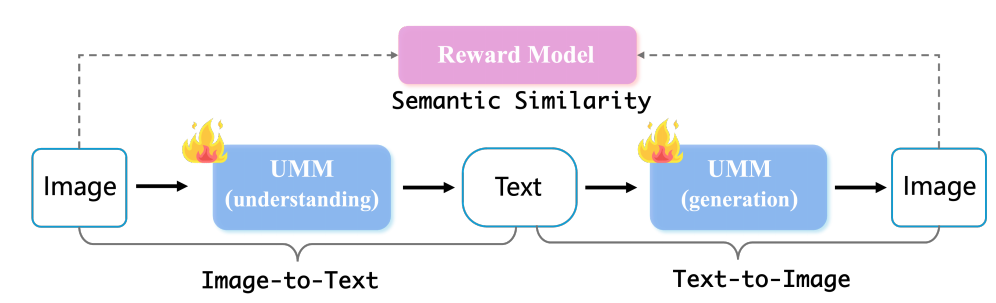
\includegraphics{images/image-0054.png}
\caption{UAE 将图像理解与图像生成串成自编码器式训练流水线}
\end{figure}

\begin{figure}[htbp]
\centering
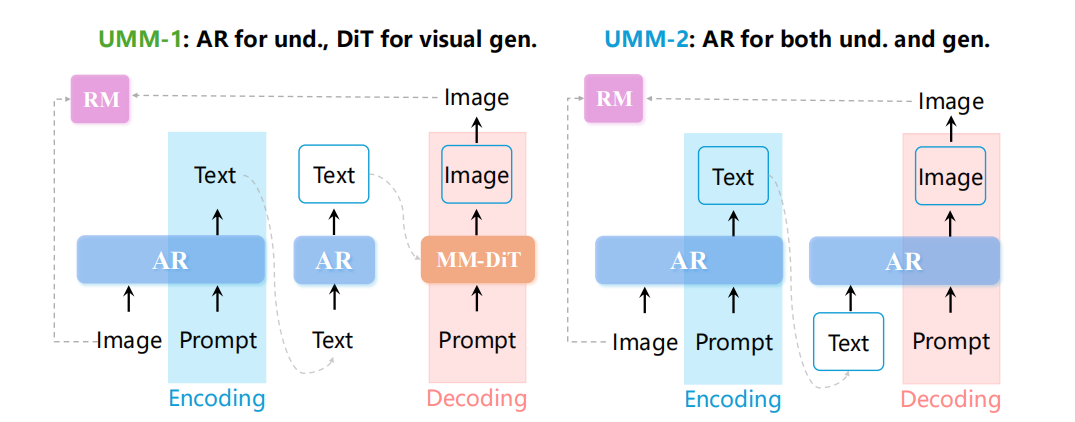
\includegraphics{images/image-0055.png}
\caption{UAE 中 UMM-1 与 UMM-2 两类统一多模态模型的编码和解码方式}
\end{figure}

\hypertarget{ux4e8cux8badux7ec3ux6d41ux7a0b}{%
\subsection{二、训练流程}\label{ux4e8cux8badux7ec3ux6d41ux7a0b}}

\hypertarget{ux4e00umm-1ux7c7bux6a21ux578b}{%
\subsubsection{（一）UMM-1类模型}\label{ux4e00umm-1ux7c7bux6a21ux578b}}

冻结Decoder（即Diffusion Transformer），将其作为RL环境的一部分，只用GRPO训练Encoder（即自回归模型）。Encoder中的ViT也要冻结，因为ViT负责把原始图像像素转化为视觉 token，是LLM的``眼睛''，一旦视觉特征在RL中发生漂移，整个系统将失去稳定基准。消融实验表明，如果对视觉编码器（ViT）或DiT也做梯度更新，RL的随机性和高方差梯度会导致生成崩溃，表现为语义信息丢失、结构坍塌、出现异常伪影等。

在训练的过程中，针对Encoder生成的每一条文本，提取其最后一个隐状态向量，通过一个投影层将其映射为扩散模型的条件输入。模型会学会在表示文段生成结束的最后一个 token中蕴含丰富的全局语义信息。

\hypertarget{ux4e8cumm-2ux7c7bux6a21ux578b}{%
\subsubsection{（二）UMM-2类模型}\label{ux4e8cumm-2ux7c7bux6a21ux578b}}

Encoder和Decoder完全相同，故同步训练。梯度（或相对优势估计）不仅会指导模型如何更好地提取语义，还会直接指导模型如何更精准地将文本翻译回视觉token。这样可以真正实现协同进化：理解能力的提升为生成提供了更密集的先验信号，而生成过程为了达到极高的还原度，反过来促使模型在统一的权重空间内完善其细粒度的视觉感知能力（例如对小目标或细微属性的捕捉）。

Encoder中的ViT也需要冻结，原因与前面所述相同。

\hypertarget{ux4e09ux4f7fux7528rlux7684ux539fux56e0ux548cux5956ux52b1ux51fdux6570}{%
\subsection{三、使用RL的原因和奖励函数}\label{ux4e09ux4f7fux7528rlux7684ux539fux56e0ux548cux5956ux52b1ux51fdux6570}}

由于``模型需要生成怎样的文本''没有可学习的Ground Truth，只通过图像生成情况好坏来评判，故这里使用强化学习中的GRPO算法，而不是监督学习或无监督学习。奖励计算方式如下：

具体操作是：使用预训练的 CLIP 模型分别提取原始输入图像 \(x\) 和重建图像 \(\tilde{x}^{(i)}\) 的视觉特征向量，并计算二者之间的余弦相似度作为单次采样的奖励值 \(\mathcal{R}\)：

\[
\mathcal{R}(x, \tilde{x}) = \cos\left(f_{\mathrm{CLIP}}(x), f_{\mathrm{CLIP}}(\tilde{x})\right)
\]

这样做有两个原因：

\begin{itemize}
\tightlist
\item
  不使用传统的像素级均方误差（MSE），是因为该框架中的``中间隐空间''是纯文本字典，文本只能保留语义级特征，例如物体、颜色和位置，无法保留光照、噪点、微小纹理等底层像素变化。如果强制用 MSE 作为奖励，算法会严重惩罚新图像和原图在底层像素上的变化，违背评估``语义一致性''的初衷。
\item
  使用 CLIP，是因为 CLIP 擅长在高维空间对齐高级语义。最大化 CLIP 相似度只要求重建图像和原图在核心属性与空间关系上吻合，这更接近``模型是否全面理解图像''的评估目标。
\end{itemize}

\hypertarget{ux53c2ux8003ux6587ux732e-200}{%
\subsection{参考文献}\label{ux53c2ux8003ux6587ux732e-200}}

\begin{itemize}
\tightlist
\item
  Yan, Z., Lin, K., Li, Z., Ye, J., Han, H., Wang, Z., Liu, H., Lin, B., Li, H., Xu, X., Xiao, X., Wang, J., Wang, H., \& Yuan, L. (2025). \href{https://arxiv.org/abs/2509.09666}{Unified Multimodal Models as Auto-Encoders}. arXiv:2509.09666.
\end{itemize}

\clearpage

\hypertarget{visionbananaux7528ux89c6ux89c9ux751fux6210ux7edfux4e00ux7406ux89e3ux4efbux52a1ux8bbaux6587}{%
\section{VisionBanana：用视觉生成统一理解任务（论文）}\label{visionbananaux7528ux89c6ux89c9ux751fux6210ux7edfux4e00ux7406ux89e3ux4efbux52a1ux8bbaux6587}}

\begin{quote}
本文是论文阅读笔记，内容代表对应论文方法或作者理解，不应直接视为领域共识或工程最佳实践。
\end{quote}

\hypertarget{ux4e00ux95eeux9898ux80ccux666f-15}{%
\subsection{一、问题背景}\label{ux4e00ux95eeux9898ux80ccux666f-15}}

目前的图像生成和图像理解还难以统一到一个模型中，实践中常常会发现二者的梯度是冲突的。但这和我们的直觉是相悖的：图像生成模型在训练时需要学会物体、场景、几何、语义、材质、空间关系等，这已经包含了对图像的理解。

对于分割、深度、法线这些视觉理解任务，过去也有人观察到生成模型偶尔能画出类似``深度图''``分割图''的东西，但这些输出格式不稳定，不能可靠解码成标准视觉任务结果，也很难拿去和专用模型公平评测。

\hypertarget{ux4e8cux6838ux5fc3ux601dux60f3-7}{%
\subsection{二、核心思想}\label{ux4e8cux6838ux5fc3ux601dux60f3-7}}

论文《Image Generators are Generalist Vision Learners》的核心贡献在于把所有视觉理解任务都重新表述成``生成一张RGB图像''，然后让图像生成器按照指令生成可解码的视觉结果。作者基于图像生成模型~Nano Banana Pro，做轻量级指令微调，得到~Vision Banana，输入原始图像+自然语言指令，输出一张RGB图像，再转换回标准视觉任务结果，例如mask、深度值、法线方向。例如，语义分割不再让模型输出类别logits，而是让模型生成一张彩色分割图：``请生成这张图的语义分割可视化图： 道路用红色，天空用蓝色，行人用黄色，背景用黑色。''模型生成RGB图后，系统根据颜色把每个像素解码成类别。这样，分割任务就被转换成了图像生成任务。

这和大语言模型的范式很像，LLM通过文本生成统一处理翻译、问答、推理、代码等任务；这篇论文则试图证明，图像生成也可以成为视觉理解任务的统一接口。分割图、深度图、法线图都可以编码成RGB图，让一个生成模型用同一种输出形式处理多种任务。Vision Banana没有为每个任务单独设计新头部、新网络或新损失，而是共享同一个生成模型，只换prompt和输出颜色编码规则。论文指出，Vision Banana在多个任务上达到或接近专用模型的水平。

\hypertarget{ux4e09ux4efbux52a1ux7c7bux522b}{%
\subsection{三、任务类别}\label{ux4e09ux4efbux52a1ux7c7bux522b}}

\hypertarget{ux4e002dux8bedux4e49ux7406ux89e3}{%
\subsubsection{（一）2D语义理解}\label{ux4e002dux8bedux4e49ux7406ux89e3}}

语义分割：给每个像素分配语义类别，例如路、人、天空、车。
实例分割：同一类别的不同物体实例要分开，例如五只狗要有五个不同mask。
指代表达分割：根据自然语言描述找出目标区域，例如``穿粉色T恤的男人''``正在伸懒腰的猫''``菜单上中英文厨师名字''。

\hypertarget{ux4e8c3dux51e0ux4f55ux7406ux89e3}{%
\subsubsection{（二）3D几何理解}\label{ux4e8c3dux51e0ux4f55ux7406ux89e3}}

单目metric depth estimation：从一张RGB图估计每个像素到相机的真实物理距离，单位是米。
surface normal estimation：估计每个像素所在表面的朝向，也就是局部3D几何方向。

\hypertarget{ux56dbux8badux7ec3ux65b9ux5f0f}{%
\subsection{四、训练方式}\label{ux56dbux8badux7ec3ux65b9ux5f0f}}

Vision Banana是在Nano Banana Pro上做轻量级指令微调。训练数据混合两部分：

原始图像生成训练数据：保持模型原本的图像生成能力。

少量视觉任务数据：教模型把视觉任务输出成指定格式的RGB图。

论文特别强调视觉任务数据比例很低，目的不是从头训练一个分割/深度模型，而是教生成器``听懂任务格式''，把它内部已有的视觉表示转成可测量输出。作者想证明的是：视觉理解能力主要来自生成式预训练，而不是来自大量任务专用微调。

\hypertarget{ux4e94ux7f16ux7801ux89c4ux5219}{%
\subsection{五、编码规则}\label{ux4e94ux7f16ux7801ux89c4ux5219}}

最简单的是分割任务。假设模型生成的图像为：

\[
G(x, y) \in [0, 255]^3
\]

其中 \(G(x, y)\) 表示像素 \((x, y)\) 的 RGB 颜色。prompt 里规定类别 \(c\) 对应颜色 \(q_c\)，那么解码时可以用最近颜色匹配：

\[
\hat{c}(x, y) = \arg\min_c \left\|G(x, y) - q_c\right\|_2
\]

意思是：对每个像素，找它生成颜色最接近哪个类别颜色，就把它归到那个类别。

实例分割稍微不同，因为实例数量事先未知，不能提前在 prompt 里指定每个实例的颜色。论文采用 per-class inference：每次只让模型分割某一类，例如``每个 garlic instance 用不同颜色表示''。模型自己给不同实例分配颜色，后处理时再根据颜色聚类，把不同颜色区域拆成不同实例。

深度估计更复杂，因为深度是实数：

\[
d \in [0, \infty)
\]

而 RGB 是有限范围：

\[
RGB \in [0, 1]^3
\]

因此作者设计了一个可逆映射，把真实深度 \(d\) 编码成 RGB 颜色。论文使用 Barron 的 power transform 先把深度压缩到 \([0, 1)\)：

\[
f(d, \lambda, c) = 1 - \left(1 - \frac{d}{\lambda c}\right)^{\lambda + 1}
\]

其中，\(d\) 是真实 metric depth，单位是米；\(\lambda\) 是形状参数，论文实验中取 \(-3\)；\(c\) 是尺度参数，论文实验中取 \(10/3\)；\(f(d,\lambda,c)\) 是归一化后的深度值，用来映射到 RGB 色彩路径上。

这样做的原因是：近处物体的深度误差通常更重要，所以映射会给近距离分配更高分辨率，远距离则被压缩。随后，论文把这个归一化深度沿 RGB 立方体边缘映射成颜色。推理时，模型生成彩色深度图，再通过反函数把颜色解码回米制深度。

表面法线更直接。法线是单位向量：

\[
\mathbf{n} = (x, y, z), \quad x, y, z \in [-1, 1]
\]

RGB 通道是 \([0, 1]\)，所以可以使用线性变换：

\[
RGB = \frac{\mathbf{n} + 1}{2}
\]

也就是：

\[
R = \frac{x + 1}{2}, \quad G = \frac{y + 1}{2}, \quad B = \frac{z + 1}{2}
\]

生成图像后再反解：

\[
\mathbf{n} = 2RGB - 1
\]

这样 RGB 图就可以表示每个像素的表面朝向。

\hypertarget{ux53c2ux8003ux6587ux732e-201}{%
\subsection{参考文献}\label{ux53c2ux8003ux6587ux732e-201}}

\begin{itemize}
\tightlist
\item
  Gabeur, V., Long, S., Peng, S., Voigtlaender, P., Sun, S., Bao, Y., Truong, K., Wang, Z., Zhou, W., Barron, J. T., Genova, K., Kannen, N., Ben, S., Li, Y., Guo, M., Yogin, S., Gu, Y., Chen, H., Wang, O., Xie, S., Zhou, H., He, K., Funkhouser, T., Alayrac, J.-B., \& Soricut, R. (2026). \href{https://arxiv.org/abs/2604.20329}{Image Generators are Generalist Vision Learners}. arXiv:2604.20329.
\end{itemize}

\clearpage

\hypertarget{uni-3darux8de8ux5c3aux5ea63dux7ed3ux6784ux7684ux7edfux4e00ux7406ux89e3ux4e0eux751fux6210ux8bbaux6587}{%
\section{Uni-3DAR：跨尺度3D结构的统一理解与生成（论文）}\label{uni-3darux8de8ux5c3aux5ea63dux7ed3ux6784ux7684ux7edfux4e00ux7406ux89e3ux4e0eux751fux6210ux8bbaux6587}}

\begin{quote}
本文是论文阅读笔记，内容代表对应论文方法或作者理解，不应直接视为领域共识或工程最佳实践。
\end{quote}

\hypertarget{ux4e00ux95eeux9898ux80ccux666f-16}{%
\subsection{一、问题背景}\label{ux4e00ux95eeux9898ux80ccux666f-16}}

长期以来，3D 结构建模在不同尺度上是割裂的：

\begin{itemize}
\tightlist
\item
  宏观与微观的壁垒：宏观模型，例如用于 3D 重建、流体力学的模型，无法直接应用于微观领域，例如蛋白质折叠、晶体生成。
\item
  任务特异性：即使在相似的尺度下，为晶体生成设计的模型也无法直接用于蛋白质折叠。这导致模型高度专业化、存在大量冗余，且无法实现数据的有效复用。
\item
  现有生成模型的局限性：主流扩散模型在微观生成中需要预先设定原子数量，而且原子类型是离散的类别分布，扩散模型难以定义完美的得分函数。
\end{itemize}

Uni-3DAR将不同尺度的3D结构用统一的通用方法表示，并统一到自回归的Next token prediction框架下，为将3D结构模态融入统一多模态理解-生成模型奠定基础。

\hypertarget{ux4e8c3dux7ed3ux6784ux8868ux793aux65b9ux6cd5}{%
\subsection{二、3D结构表示方法}\label{ux4e8c3dux7ed3ux6784ux8868ux793aux65b9ux6cd5}}

\hypertarget{ux4e00ux52a8ux6001ux7531ux7c97ux5230ux7ec6ux7684ux516bux53c9ux6811-token-ux5316}{%
\subsubsection{（一）动态由粗到细的八叉树 Token 化}\label{ux4e00ux52a8ux6001ux7531ux7c97ux5230ux7ec6ux7684ux516bux53c9ux6811-token-ux5316}}

3D 空间本质上是高度稀疏的，无论是微观分子还是宏观物体表面。如果直接使用完整的 3D 体素网格（Voxel Grid），计算量会呈指数级爆炸。Uni-3DAR 采用了基于八叉树（Octree）的无损压缩方法：

\begin{itemize}
\tightlist
\item
  空间划分：从包含整个结构的单一根节点细胞开始，递归地将空间等分为 \(2^3 = 8\) 个子细胞。
\item
  数学推导：假设根节点的边长为 \(c_0\)，则在第 \(L\) 层（深度为 \(L\)）的叶子节点边长为：
\end{itemize}

\[
c_{L-1} = \frac{c_0}{2^{L-1}}
\]

\begin{itemize}
\tightlist
\item
  自适应剪枝：只有包含实体（如原子或物体表面）的区域才会被继续划分，空的区域分支会被直接剪枝。这使得最高层最多只有 \(8^{L-1}\) 个叶子节点，而且绝大部分节点会因为稀疏性被剪去。
\end{itemize}

\hypertarget{ux4e8cux7ec6ux7c92ux5ea6ux7ed3ux6784ux8868ux793a}{%
\subsubsection{（二）细粒度结构表示}\label{ux4e8cux7ec6ux7c92ux5ea6ux7ed3ux6784ux8868ux793a}}

八叉树只能确定``哪里有东西''（占据状态），但无法描述细节。因此，在八叉树的最底层，非空叶子节点被视为 3D Patch：

\begin{itemize}
\tightlist
\item
  微观尺度（如分子）：将 Patch 大小设置为 \(c_{L-1}=0.24\,\mathrm{\mathring{A}}\)，确保每个 Patch 最多只包含一个原子。Token 包含原子类型 \(t_i\) 和在细胞内的精确连续坐标 \(e_i=(e_i^0,e_i^1,e_i^2)\)。坐标通过分辨率 \(c_r=0.01\,\mathrm{\mathring{A}}\) 离散化为 \(N_p=c_{L-1}/c_r\) 个区间。
\item
  宏观尺度：使用 VQ-VAE 将体素块量化为离散的字典 Token。
\end{itemize}

\hypertarget{ux4e09ux6838ux5fc3ux539fux7406}{%
\subsection{三、核心原理}\label{ux4e09ux6838ux5fc3ux539fux7406}}

第一阶段是动态展开``脚手架''，也就是预测空间占据。模型并不是一上来就直接预测原子，而是从宏观到微观，逐层预测空间的占据情况：

\begin{enumerate}
\def\labelenumi{\arabic{enumi}.}
\tightlist
\item
  模型一开始面对的是一个包含整个分子的巨大``根节点''细胞。
\item
  模型预测这个大细胞的 8 个子区块中哪几个有东西，这相当于前面提到的两层子树压缩的 256 分类任务。
\item
  对于预测``有东西''的子区块，模型继续往下细分，直到到达最底层（第 \(L-1\) 层，也就是边长为 \(0.24\,\mathrm{\mathring{A}}\) 的微小细胞）。
\item
  关键点在于，这一层层的细胞是模型自己刚刚自回归预测出来的，所以当它预测出``最底层的某个微小细胞 A 被占据''时，细胞 A 的中心坐标对模型来说已经是绝对已知的。
\end{enumerate}

第二阶段是在已知位置放置 \texttt{MASK} Token 并预测``细节''，也就是填补内容。此时，模型已经在空间中划分出一系列已知坐标、微小且被占据的``叶子细胞''：

\begin{enumerate}
\def\labelenumi{\arabic{enumi}.}
\tightlist
\item
  放置掩码：模型在刚才推导出的细胞 A 的中心坐标处，放置一个 \texttt{MASK} Token。因此，这个 \texttt{MASK} Token 的位置是已知的，它代表``这个极其微小的空间块''。
\item
  预测对象：既然位置已经固定在细胞 A，模型接下来要预测的内容就是这个细胞里装的是什么，包括类型 \(t_i\)，以及原子在细胞 A 内部的具体相对偏移量 \(e_i\)。
\end{enumerate}

为什么要这么做：

如果让模型直接在虚空中预测一个原子的绝对坐标，例如 \(x = 12.34, y = 5.67, z = 8.90\)，就相当于让模型``盲猜''，没有任何空间参照系。这在自回归模型中表现很差，因为上一个生成的原子和下一个生成的原子在空间上可能毫无规律可言。

Uni-3DAR 通过 MNTP（掩码下个 Token 预测）配合八叉树，把``盲猜''变成一道``填空题''：

\begin{itemize}
\tightlist
\item
  传统方式问的是：``下一个原子是什么？它在宇宙中的哪里？''这很难。
\item
  Uni-3DAR 的方式问的是：``根据刚才生成的空间轮廓，我知道坐标 \((x,y,z)\) 这里的微小细胞里一定有个东西，也就是已知位置的 \texttt{MASK} Token。请告诉我，它具体是什么原子？在这个微小细胞的哪个精确角落？''这大幅降低了预测难度。
\end{itemize}

\hypertarget{ux56dbux63a8ux7406ux5de5ux4f5cux6d41}{%
\subsection{四、推理工作流}\label{ux56dbux63a8ux7406ux5de5ux4f5cux6d41}}

推理时可以理解为以下循环：

\begin{itemize}
\tightlist
\item
  第 0 步（起点）：系统在 3D 宇宙中心放置一个代表最高层（Root）的 \texttt{MASK} Token，位置绝对已知。
\item
  第 1 步（预测第 0 层）：模型看着这个 \texttt{MASK} Token，结合条件（例如分子化学式），预测出它的内容，例如 \texttt{10000001}（假设转换为十进制是 129）。
\item
  第 2 步（几何推导位置）：系统读取 \texttt{10000001}，立刻知道这个大空间的第 1 号角落和第 8 号角落有东西。系统随即通过几何公式计算出这两个子角落的精确中心坐标。
\item
  第 3 步（放置新的 \texttt{MASK} Token）：系统在刚刚算出的两个精确坐标处，放置两个属于第 1 层的 \texttt{MASK} Token。
\item
  第 4 步（预测第 1 层）：模型再去预测这两个新 \texttt{MASK} Token 的内容（0 到 255）。
\item
  循环往复：预测内容、解码出子节点占据情况、算出子节点确切坐标、在新坐标放置 \texttt{MASK} Token、继续预测新内容。
\item
  终局（到达最底层）：当这个过程循环到预设的八叉树最底层，例如第 6 层、细胞边长 \(0.24\,\mathrm{\mathring{A}}\) 时，系统放置的 \texttt{MASK} Token 就不再是 0 到 255 的分类任务，而是切换成原子级预测头。模型在这个微小细胞的 \texttt{MASK} Token 处，预测具体的原子类型（碳、氢、氧等）和在细胞内的微调坐标 \(e_i\)。
\end{itemize}

\hypertarget{ux4e94ux8badux7ec3ux65b9ux6cd5}{%
\subsection{五、训练方法}\label{ux4e94ux8badux7ec3ux65b9ux6cd5}}

\hypertarget{ux4e00ux6574ux4f53ux8badux7ec3ux8303ux5f0fteacher-forcing-ux4e0bux7684ux586bux7a7aux9898}{%
\subsubsection{（一）整体训练范式：Teacher Forcing 下的``填空题''}\label{ux4e00ux6574ux4f53ux8badux7ec3ux8303ux5f0fteacher-forcing-ux4e0bux7684ux586bux7a7aux9898}}

和 GPT 等大语言模型的训练方式类似，Uni-3DAR 在训练时采用 Teacher Forcing（教师强制）机制。在训练阶段，模型其实是在``看着正确答案''学习。系统会将真实的 3D 结构完整地转换为八叉树加原子的 Token 序列，并在所有应该预测的位置打上 \texttt{MASK} Token。模型需要同时对序列中的所有 \texttt{MASK} Token 进行预测，计算预测分布与真实内容之间的差距（Loss），然后反向传播更新权重。

\hypertarget{ux4e8cux5b8fux89c2ux9aa8ux67b6ux7684ux8badux7ec3ux516bux53c9ux6811-token-ux9884ux6d4b}{%
\subsubsection{（二）宏观骨架的训练：八叉树 Token 预测}\label{ux4e8cux5b8fux89c2ux9aa8ux67b6ux7684ux8badux7ec3ux516bux53c9ux6811-token-ux9884ux6d4b}}

对于八叉树中间节点的 \texttt{MASK} Token，模型的训练目标是预测它的 8 个子节点是否存在：

\begin{itemize}
\tightlist
\item
  损失函数：标准的 256 分类交叉熵损失（Cross-Entropy Loss）。
\item
  这一阶段让模型学习如何根据化学式或整体轮廓，正确地``开疆拓土''。
\end{itemize}

\hypertarget{ux4e09ux5e95ux90e8ux539fux5b50ux7684ux8badux7ec3ux7ec6ux8282ux5faeux89c2ux7ec6ux7c92ux5ea6ux9884ux6d4b}{%
\subsubsection{（三）底部原子的训练细节：微观细粒度预测}\label{ux4e09ux5e95ux90e8ux539fux5b50ux7684ux8badux7ec3ux7ec6ux8282ux5faeux89c2ux7ec6ux7c92ux5ea6ux9884ux6d4b}}

当序列推进到八叉树的最底层，也就是叶子节点细胞、边长 \(0.24\,\mathrm{\mathring{A}}\) 时，这里的 \texttt{MASK} Token 对应的真实内容是一个具体原子。对这个底层 \texttt{MASK} Token 的训练被拆解为更细的步骤：

\begin{enumerate}
\def\labelenumi{\arabic{enumi}.}
\tightlist
\item
  预测原子类型 \(t_i\)：模型首先看着底层 \texttt{MASK} Token，预测这个微小细胞里装的是什么原子，例如碳、氢、氧等。这仍然是标准分类任务，使用交叉熵损失。
\item
  预测细胞内连续坐标 \(e_i\)：确定原子类型后，还要确定它在这个极小细胞内的精确相对位置。因为坐标是连续值，直接回归比较难，Uni-3DAR 采用更像语言模型的做法：先将连续坐标按照 \(0.01\,\mathrm{\mathring{A}}\) 的高分辨率离散化，切分成整数索引 \(0\) 到 \(N_p-1\)；再采用内部自回归方式预测坐标，先预测 \(x\) 坐标分类概率，再用真实的 \(x\) 坐标作为条件预测 \(y\) 坐标，最后用真实的 \(x,y\) 坐标作为条件预测 \(z\) 坐标。
\end{enumerate}

\(x,y,z\) 的预测也被视为离散分类任务，会产生 3 个交叉熵损失。论文也提到，可以使用 Token 级别的 Diffusion 扩散损失来预测连续坐标，但由于自回归分类的方式更高效且效果相当，所以默认采用自回归预测坐标。

这样，就可以将3D结构生成统一到Next token prediction的框架下。

\hypertarget{ux56dbux635fux5931ux7684ux6c47ux805a}{%
\subsubsection{（四）损失的汇聚}\label{ux56dbux635fux5931ux7684ux6c47ux805a}}

在一次训练迭代中，模型实际会计算整个序列中所有掩码的损失之和：

\textbf{总损失 = 所有八叉树节点的 256 分类 Loss + 所有底部原子的类型 Loss + 所有底部原子的 X、Y、Z 坐标 Loss。}

\hypertarget{ux53c2ux8003ux6587ux732e-202}{%
\subsection{参考文献}\label{ux53c2ux8003ux6587ux732e-202}}

\begin{itemize}
\tightlist
\item
  Lu, S., Lin, H., Yao, L., Gao, Z., Ji, X., E, W., Zhang, L., \& Ke, G. (2025). \href{https://arxiv.org/abs/2503.16278}{Uni-3DAR: Unified 3D Generation and Understanding via Autoregression on Compressed Spatial Tokens}. arXiv:2503.16278.
\end{itemize}

\clearpage


% 结合世界模型的具身智能
\hypertarget{ux7ed3ux5408ux4e16ux754cux6a21ux578bux7684ux5177ux8eabux667aux80fd}{%
\chapter{结合世界模型的具身智能}\label{ux7ed3ux5408ux4e16ux754cux6a21ux578bux7684ux5177ux8eabux667aux80fd}}

\hypertarget{ux7ed3ux5408ux4e16ux754cux6a21ux578bux7684ux5177ux8eabux667aux80fdux6982ux8ff0}{%
\section{结合世界模型的具身智能概述}\label{ux7ed3ux5408ux4e16ux754cux6a21ux578bux7684ux5177ux8eabux667aux80fdux6982ux8ff0}}

\hypertarget{ux4e00ux95eeux9898ux80ccux666f-17}{%
\subsection{一、问题背景}\label{ux4e00ux95eeux9898ux80ccux666f-17}}

尽管 VLA 具有强大的语义推理能力，但具身智能本质上是在物理世界而非数字世界中运行的，这就需要在物理世界而非数字世界中对未来状态进行预测，以实现规划，根据规划输出最终动作。因此，我们需要整合输出下一状态的世界模型与输出动作的策略模型。

\hypertarget{ux4e8cux6838ux5fc3ux6982ux5ff5-1}{%
\subsection{二、核心概念}\label{ux4e8cux6838ux5fc3ux6982ux5ff5-1}}

\hypertarget{ux4e16ux754cux6a21ux578bux7684ux5b9aux4e49}{%
\subsubsection{1. 世界模型的定义}\label{ux4e16ux754cux6a21ux578bux7684ux5b9aux4e49}}

世界模型的核心是构建一个内部表征来捕捉环境的动态演化。它被定义为一个映射函数，输入过去的状态 \(s\) 和（可选的）未来动作 \(a\)，输出预测的未来状态。公式表示为：

\[
s_{[t,t+k]} = M_{\theta}^{WM}\left(s_{[t-h,t-1]}, a_{[t,t+k]}\right)
\]

\begin{itemize}
\tightlist
\item
  \textbf{无动作条件的世界模型（Action-Free）}：仅依靠历史和高层语言指令进行预测，常作为``想象引擎''支持高层决策。
\item
  \textbf{动作条件的世界模型（Action-Conditioned）}：需要输入具体的未来动作序列，充当可学习的物理模拟器，用于评估具体策略的后果。
\end{itemize}

\hypertarget{ux7b56ux7565ux6a21ux578bux7684ux5b9aux4e49}{%
\subsubsection{2. 策略模型的定义}\label{ux7b56ux7565ux6a21ux578bux7684ux5b9aux4e49}}

具身智能任务通常被建模为部分可观察马尔可夫决策过程（POMDP）。智能体的目标是学习一个策略 \(\pi\)，通过基于历史信息 \(I_t\)（包括历史视觉观察 \(o_{1:t}\)、历史动作 \(a_{1:t-1}\) 以及语言指令 \(L\)）选择动作 \(a_t\)，来最大化累积奖励 \(R\)。公式表示为：

\[
\pi^* = \arg\max_{\pi}\mathbb{E}\left[\sum_{t=0}^{T} R(s_t, a_t)\mid \pi, I_t\right]
\]

\hypertarget{ux4e09ux4e16ux754cux6a21ux578bwmux4e0eux7b56ux7565ux6a21ux578bpmux7684ux7ed3ux5408ux65b9ux5f0f}{%
\subsection{三、世界模型（WM）与策略模型（PM）的结合方式}\label{ux4e09ux4e16ux754cux6a21ux578bwmux4e0eux7b56ux7565ux6a21ux578bpmux7684ux7ed3ux5408ux65b9ux5f0f}}

根据策略的优化目标产生的梯度能不能直接反向传播到世界模型里，以及在推理的一个前向过程中，策略输出动作时是否显式依赖于世界模型预测的状态，可将世界模型（WM）与策略模型（PM，一般为LLM）的结合方式分为以下三种：

\begin{enumerate}
\def\labelenumi{\arabic{enumi}.}
\tightlist
\item
  解耦模块化架构
\end{enumerate}

世界模型和策略模型是相对分离但协同工作的独立模块。策略模型在核心计算步骤不依赖世界模型的预测输出，策略模型的梯度不回传到世界模型，即：

\[
a_t = \mathrm{Policy}(s_t)
\]

主要类别：（在``世界模型与语言模型解耦的物理世界推理''部分）

（1）作为训练环境：策略在世界模型的``想象''中运行。

（2）推理时并行展开：策略模块先并行生成一批候选轨迹，再由世界模型预测这些动作的未来价值，最终选择高价值动作。

（3）推理时树搜索展开：策略模块在世界模型中进行蒙特卡洛树搜索等规划，最终选择动作。

\begin{enumerate}
\def\labelenumi{\arabic{enumi}.}
\setcounter{enumi}{1}
\tightlist
\item
  顺序架构
\end{enumerate}

先由世界模型在没有底层动作输入的情况下，想象出一个有价值的未来状态，然后策略模型制定、执行策略达到该状态。此时策略依赖于世界模型的输出，策略模型的梯度会回传给世界模型，即：

\[
a_t = \mathrm{Policy}(s_t, \hat{s}_{t+k}), \quad \text{where } \hat{s}_{t+k} = WM(s_t)
\]

\begin{itemize}
\tightlist
\item
  \textbf{主要类别}（基于 WM 传递给策略的状态形式）：

  \begin{itemize}
  \tightlist
  \item
    \textbf{神经未来态（Neural Future States）}：从视频生成模型中提取中间层特征（如 U-Net 的上采样层特征）作为条件信号传递给扩散策略。
  \item
    \textbf{显式潜在态（Explicit Latent Future States）}：通过自监督学习提取结构化的潜在表征（Latent Representations），过滤视觉冗余，更利于决策对齐。
  \item
    \textbf{像素级视觉态（Pixel-level Future States）}：利用视频生成模型直接合成未来的 RGB 图像帧或视频，使策略能在直观的观察空间中进行推理（如生成目标图像再用逆动力学模型执行）。
  \end{itemize}
\end{itemize}

\begin{enumerate}
\def\labelenumi{\arabic{enumi}.}
\setcounter{enumi}{2}
\tightlist
\item
  统一架构（统一多模态生成模型）
\end{enumerate}

世界模型和策略模型融合为一个单一的端到端神经网络，模型同时进行未来状态预测和动作生成，即：

\[
\left(s_{\{t,t+k\}}, a_{\{t,t+k\}}\right) = M_Y^{unified}\left(s_{\{t-h,t-1\}}, l[, a_{\{t-h,t-1\}}]\right)
\]

\begin{itemize}
\tightlist
\item
  \textbf{主要类别}：

  \begin{itemize}
  \tightlist
  \item
    \textbf{视觉作为未来态（Vision as Future States）}：利用自回归 Transformer 或扩散模型（Diffusion Models）联合生成视觉标记（如 RGB、深度图或点云）和动作标记。这种方法能提供密集且时间连贯的场景动态观察。
  \item
    \textbf{语言作为未来态（Language as Future States）}：建立在大型语言模型（LLM/VLM）的基础上，利用其强大的高级推理能力，通过自然语言来描述环境变化或机器人的未来抽象状态。
  \end{itemize}
\end{itemize}

这本质上就是统一多模态生成模型（多模态理解-生成一体化）。

具体类型上又分为：（1）多头同时生成状态和动作；（2）在CoT中交替生成状态和动作。

总的来说，解耦模块化架构拥有极高的可解释性和组件复用性；顺序架构支持长视距的分层推理、规划和想象；统一架构则实现了紧密的预测-控制协调与联合优化。三者各有优点。

\hypertarget{ux53c2ux8003ux6587ux732e-203}{%
\subsection{参考文献}\label{ux53c2ux8003ux6587ux732e-203}}

\begin{itemize}
\tightlist
\item
  Ha, D., \& Schmidhuber, J. (2018). \href{https://arxiv.org/abs/1803.10122}{World Models}. arXiv:1803.10122.
\item
  LeCun, Y. (2022). \href{https://openreview.net/forum?id=BZ5a1r-kVsf}{A Path Towards Autonomous Machine Intelligence}. OpenReview.
\item
  Battaglia, P. W., Hamrick, J. B., \& Tenenbaum, J. B. (2013). \href{https://www.pnas.org/doi/10.1073/pnas.1306572110}{Simulation as an Engine of Physical Scene Understanding}. Proceedings of the National Academy of Sciences.
\end{itemize}

\clearpage

\hypertarget{ux4e16ux754c-ux7b56ux7565ux89e3ux8026ux67b6ux6784ux7684ux5177ux8eabux667aux80fdux8bbaux6587}{%
\section{世界-策略解耦架构的具身智能（论文）}\label{ux4e16ux754c-ux7b56ux7565ux89e3ux8026ux67b6ux6784ux7684ux5177ux8eabux667aux80fdux8bbaux6587}}

\begin{quote}
本文是论文阅读笔记，内容代表对应论文方法或作者理解，不应直接视为领域共识或工程最佳实践。
\end{quote}

\hypertarget{ux4e00ux4e16ux754cux6a21ux578bux4f5cux4e3aux5177ux8eabux7b56ux7565ux6a21ux578bux7684ux8badux7ec3ux4e0eux8bc4ux6d4bux73afux5883}{%
\subsection{一、世界模型作为具身策略模型的训练与评测环境}\label{ux4e00ux4e16ux754cux6a21ux578bux4f5cux4e3aux5177ux8eabux7b56ux7565ux6a21ux578bux7684ux8badux7ec3ux4e0eux8bc4ux6d4bux73afux5883}}

\hypertarget{ux4e00ux95eeux9898ux80ccux666f-18}{%
\subsubsection{（一）问题背景}\label{ux4e00ux95eeux9898ux80ccux666f-18}}

随着通用机器人策略（如基于大模型的 Vision-Language-Action 策略）的发展，这类策略已经能够通过自然语言指令在多种环境中执行任务，但评估它们仍然困难：

\begin{enumerate}
\def\labelenumi{\arabic{enumi}.}
\tightlist
\item
  硬件评估成本高且存在风险：在真实硬件上覆盖所有标称场景和边缘场景并不现实。特别是评估``语义安全性''（Semantic Safety，例如不把塑料放在炉子上）时，真实测试可能危及机器人、环境或人类。
\item
  传统物理模拟器存在局限：传统模拟器需要人工创建逼真的资产，难以精确模拟非刚体和接触动力学，并且存在明显的 Sim-to-Real 视觉差异。
\end{enumerate}

可以利用世界模型作为测试具身策略的环境，利用其在海量网络视频上训练获得的生成能力，来替代物理引擎进行仿真。在具身智能的训练方法从以模仿学习为主转向与 RL 结合的背景下，这一点尤其重要。

\hypertarget{ux4e8cux6838ux5fc3ux65b9ux6cd5}{%
\subsubsection{（二）核心方法}\label{ux4e8cux6838ux5fc3ux65b9ux6cd5}}

以 Google 的研究为例，为了让视频生成模型理解机器人动作，可在覆盖多种操作技能和场景的大规模机器人数据集上对 Veo 进行微调，随后利用该世界模型作为评估机器人策略的环境。

该视频模拟器评估策略的完整工作流如下：

\begin{enumerate}
\def\labelenumi{\arabic{enumi}.}
\tightlist
\item
  场景初始化与编辑：获取真实世界的一帧初始 RGB 图像。如果需要进行分布外（OOD）评估或安全红队测试，系统使用图像生成模型根据语言描述对初始帧进行生成式编辑，例如添加新物体或改变背景。
\item
  多视角合成：由于 ALOHA 2 机器人包含顶视、侧视、左右手腕等多个摄像头，系统使用微调后的 Veo 2 模型，仅凭单一俯视编辑图像合成其他视角的初始观测图像。
\item
  策略推出：将合成的多视角初始帧和任务指令输入待评估的机器人策略，例如基于 Gemini Robotics On-Device 的策略。策略输出未来的一系列机器人位姿。
\item
  视频生成：微调后的 Veo Robotics 模型以当前图像观测和未来机器人位姿序列为条件，自回归生成连续的未来视频帧。
\item
  结果判定：人类评估员对生成的 8 秒视频进行成功或失败的二元打分，以此预测策略在真实世界中的表现。
\end{enumerate}

\hypertarget{ux4e09ux5757ux7ea7ux9884ux6d4b}{%
\subsubsection{（三）块级预测}\label{ux4e09ux5757ux7ea7ux9884ux6d4b}}

世界状态预测（视频生成）需要消耗的算力显著大于动作预测需要的算力，因此不必总是逐帧预测，而可以采用块级预测。

具体来说：

\begin{enumerate}
\def\labelenumi{\arabic{enumi}.}
\tightlist
\item
  状态采样：系统从包含真实交互记录的离线经验回放缓冲区 \(D\) 中采样一个历史观测状态作为起始点 \(s_t\)。
\item
  动作预测：VLA 策略模型接收当前状态 \(s_t\) 和任务语言指令 \(l\)，一次性预测一个包含 \(k\) 个连续动作的动作切块：
\end{enumerate}

\[
\bar{a}_t = (a_t, a_{t+1}, \ldots, a_{t+k-1})
\]

\begin{enumerate}
\def\labelenumi{\arabic{enumi}.}
\setcounter{enumi}{2}
\tightlist
\item
  直接跳跃预测：UMM-World 不逐帧渲染 \(s_{t+1}, s_{t+2}, \ldots, s_{t+k-1}\) 的中间过程，而是直接建模条件概率 \(p(s_{t+k} \mid s_t, \bar{a}_t)\)，一步输出执行完整动作切块后的第 \(t+k\) 帧图像。
\end{enumerate}

\hypertarget{ux56dbux4ea4ux9519ux89c6ux89d2ux89e3ux7801}{%
\subsubsection{（四）交错视角解码}\label{ux56dbux4ea4ux9519ux89c6ux89d2ux89e3ux7801}}

机器人往往有多个摄像头，这些摄像头获得的图像信息必须满足三维一致性，即共同构成同一个一致的三维世界。为了解决多视角一致性问题，UMM-World 等方法不独立生成每个视角的图像，而是将头部视角、腕部视角等放在同一个序列中交错解码：每次先生成其中一个视角，再把该视角图像放入上下文，以此作为条件生成下一个视角，依此类推。

\hypertarget{ux4e94ux5757ux7ea7ux5956ux52b1ux8bc4ux4f30}{%
\subsubsection{（五）块级奖励评估}\label{ux4e94ux5757ux7ea7ux5956ux52b1ux8bc4ux4f30}}

目前，生成式世界模型仍存在误差累积问题。而很多机器人任务是稀疏奖励的，很小的视觉偏差就可能把一个状态从成功翻成失败，或者相反，这对强化学习影响很大。短期内为避免该问题，可采取块级奖励评估：每完成一个小块的动作，就给予奖励。

生成 \(s_{t+k}\) 的图像后，UMM-World 会立即切换身份，充当视觉-语言任务裁判（Reward Model）：

\begin{enumerate}
\def\labelenumi{\arabic{enumi}.}
\tightlist
\item
  系统向 UMM-World 输入结构化提示词，例如``仔细检查物体状态，判断任务是否成功完成，必须回答 Yes 或 No''。
\item
  模型根据新生成图像回答 Yes 或 No，从而输出二元奖励信号。
\item
  这个块级奖励等效于该动作块中每个单步奖励的贴现总和：
\end{enumerate}

\[
r_\theta(s_t, \bar{a}_t, l) = \sum_{i=1}^{k} \gamma^{i-1} r(s_{t+i}, l)
\]

连续推演时，生成的未来状态 \(s_{t+k}\) 会作为新的起点反馈给 VLA 模型，VLA 继续预测下一块动作，UMM-World 再预测 \(s_{t+2k}\)。如此循环多次，形成一条由世界模型想象出来的合成交互轨迹。最终，算法使用 Flow-Noise 这类 PPO 变体在大幅缩短视界的合成轨迹上计算优势函数，并更新 VLA 模型的权重参数，完成一次策略迭代。

\hypertarget{ux516dux53cdux6620ux4e16ux754cux6a21ux578bux8bc4ux4f30ux673aux5668ux4ebaux51c6ux786eux6027ux7684ux6307ux6807}{%
\subsubsection{（六）反映世界模型评估机器人准确性的指标}\label{ux516dux53cdux6620ux4e16ux754cux6a21ux578bux8bc4ux4f30ux673aux5668ux4ebaux51c6ux786eux6027ux7684ux6307ux6807}}

以 Google 的研究为例，常用如下指标。

\begin{enumerate}
\def\labelenumi{\arabic{enumi}.}
\tightlist
\item
  MMRV
\end{enumerate}

MMRV 用于衡量``视频模型预测的策略排名''和``真实世界测得的策略排名''之间的一致性。较低的 MMRV 表示较高的排名一致性，其取值范围为 \([0, 1]\)。给定 \(n\) 个不同机器人策略 \(\pi_1, \ldots, \pi_n\)，它们在真实世界中的成功率记为 \(R_1^{\mathrm{real}}, \ldots, R_n^{\mathrm{real}}\)，在视频模拟器中预测的成功率记为 \(R_1^{\mathrm{pred}}, \ldots, R_n^{\mathrm{pred}}\)，MMRV 定义为：

\[
\mathrm{MMRV}
= \frac{1}{n} \sum_{i=1}^{n} \max_{1 \le j \le n}
\mathrm{RankViolation}(i, j)
\]

其中，秩违反度定义为：

\[
\mathrm{RankViolation}(i, j)
= \left|R_i^{\mathrm{real}} - R_j^{\mathrm{real}}\right|
\cdot
\mathbf{1}\left[
(R_i^{\mathrm{pred}} \lt R_j^{\mathrm{pred}})
\ne
(R_i^{\mathrm{real}} \lt R_j^{\mathrm{real}})
\right]
\]

\(\mathbf{1}[\cdot]\) 是指示函数。如果视频模型对策略 \(i\) 和策略 \(j\) 的强弱排序预测与真实世界中的实际排序不一致，则该函数值为 \(1\)；若一致则为 \(0\)。\(\left|R_i^{\mathrm{real}} - R_j^{\mathrm{real}}\right|\) 表示两个策略在真实世界中成功率的实际差距。因此，MMRV 惩罚的是那些``实际性能差距很大，却被模拟器排错序''的情况；如果两个策略实际表现很接近而被排错，惩罚会相对较小。

\begin{enumerate}
\def\labelenumi{\arabic{enumi}.}
\setcounter{enumi}{1}
\tightlist
\item
  预测成功率与真实成功率之间的线性相关程度：可用皮尔逊相关系数等量化。
\end{enumerate}

\hypertarget{ux4e8cux7b56ux7565ux6a21ux578bux5728ux4e16ux754cux6a21ux578bux4e2dux5c55ux5f00-mcts}{%
\subsection{二、策略模型在世界模型中展开 MCTS}\label{ux4e8cux7b56ux7565ux6a21ux578bux5728ux4e16ux754cux6a21ux578bux4e2dux5c55ux5f00-mcts}}

\hypertarget{ux4e00ux6838ux5fc3ux601dux60f3-27}{%
\subsubsection{（一）核心思想}\label{ux4e00ux6838ux5fc3ux601dux60f3-27}}

传统的基于模型的强化学习（Model-based RL）试图通过学习来重建整个环境状态或视觉像素流。潜变量动力学路线将其简化为生成环境对应的潜变量，但由于存在视觉重建损失，事实上仍然试图压缩学习环境的所有要素，可能把模型容量浪费在与规划决策无关的视觉细节上。

将世界模型直接用于搜索规划的路线放弃了``重建真实环境''的执念。在智能体系统中，策略网络先运用蒙特卡洛树搜索等规划算法进行推演规划，再在现实世界中执行行动。这里世界模型用于 MCTS 阶段，完全服务于规划。

MuZero 是这种范式的初始形态。世界模型内部构建的``隐藏状态''没有任何特定环境语义约束，只要这个隐式状态能准确预测对规划最直接相关的三个核心量即可：奖励（Reward）、策略（Policy）和价值（Value）。

\hypertarget{ux4e8cux6a21ux578bux67b6ux6784-5}{%
\subsubsection{（二）模型架构}\label{ux4e8cux6a21ux578bux67b6ux6784-5}}

MuZero 主要包含三个函数。

\begin{enumerate}
\def\labelenumi{\arabic{enumi}.}
\tightlist
\item
  表征函数 \(h\)：将过去的真实历史观测值，如连续棋盘画面或 Atari 游戏画面 \(o_1, \ldots, o_t\)，映射为初始隐藏状态 \(s^0\)。它是内部规划的起点：
\end{enumerate}

\[
s^0 = h_\theta(o_1, \ldots, o_t)
\]

\begin{enumerate}
\def\labelenumi{\arabic{enumi}.}
\setcounter{enumi}{1}
\tightlist
\item
  动态函数 \(g\)：负责在模型内部模拟环境动态转移。给定上一隐藏状态 \(s^{k-1}\) 和当前假设动作 \(a^k\)，生成下一隐藏状态 \(s^k\) 并预测即时奖励 \(r^k\)：
\end{enumerate}

\[
r^k, s^k = g_\theta(s^{k-1}, a^k)
\]

\begin{enumerate}
\def\labelenumi{\arabic{enumi}.}
\setcounter{enumi}{2}
\tightlist
\item
  预测函数 \(f\)：负责对当前局势进行评估。根据当前隐藏状态 \(s^k\)，预测该状态下的动作选择策略 \(p^k\) 以及价值函数 \(v^k\)：
\end{enumerate}

\[
p^k, v^k = f_\theta(s^k)
\]

这里只对环境观测进行了嵌入处理，事实上也可以将动作编码为隐空间中的特征向量，让物理结果相似的动作在嵌入空间中被拉近，从而赋予智能体更强的泛化能力。它在测试某个动作时学到的规律，能够自动泛化到特征空间相邻的其他动作上，提升学习效率。

在连续控制任务中，策略网络的输出也可以采用高斯分布来表示连续动作空间中的策略。

输入处理网络可按输入形态设计：

\begin{enumerate}
\def\labelenumi{\arabic{enumi}.}
\tightlist
\item
  二维图像输入（Vision）：对于 Atari 或基于摄像头的视觉控制任务，Ez-V2 基本沿用了 EfficientZero 验证过的高效残差卷积架构。
\item
  一维状态输入（Proprio Control）：为了处理连续控制中的低维向量输入，如关节角度和速度，Ez-V2 将卷积层替换为全连接层，并引入运行均值模块（Running mean block）归一化输入特征，采用 Pre-LN Transformer 风格的残差模块防止梯度爆炸并提升表达能力。
\end{enumerate}

\hypertarget{ux4e09ux4e3aux4ec0ux4e48ux52a8ux6001ux51fdux6570ux662fux786eux5b9aux6027ux7684ux800cux4e0dux50cf-ssm-ux90a3ux6837ux5b58ux5728ux968fux673aux91c7ux6837}{%
\subsubsection{（三）为什么动态函数是确定性的，而不像 SSM 那样存在随机采样}\label{ux4e09ux4e3aux4ec0ux4e48ux52a8ux6001ux51fdux6570ux662fux786eux5b9aux6027ux7684ux800cux4e0dux50cf-ssm-ux90a3ux6837ux5b58ux5728ux968fux673aux91c7ux6837}}

RSSM 的核心任务是重建和预测未来的实际观测，如像素画面。如果环境存在随机性，确定性网络往往会输出所有可能未来的``模糊平均值''，因此 RSSM 必须引入隐式随机变量来学习真实环境的概率分布。

而 MuZero 走的是``价值等价''路线。它的内部隐藏状态没有任何具体环境状态的语义约束。这个隐藏状态存在的唯一目的，是准确预测未来相关的三个量：策略、价值和奖励。既然价值在强化学习中本身就是对未来累计收益的数学期望，确定性的动态模型只需要学会转移到一个能够正确输出期望价值的抽象状态即可，不需要像 RSSM 那样精确采样还原每一条随机物理分支。

同时，MuZero 高度依赖 MCTS 进行规划。MCTS 中状态转移通常按确定性路径展开，随机性主要存在于动作选择阶段。如果给定动作后的环境反馈也需要随机展开，就会变成随机树搜索，计算量大幅增加。

\hypertarget{ux56dbux7b97ux6cd5ux5de5ux4f5cux6d41}{%
\subsubsection{（四）算法工作流}\label{ux56dbux7b97ux6cd5ux5de5ux4f5cux6d41}}

MuZero 在世界模型中进行蒙特卡洛树搜索，而在真实环境中执行实际行动，每次行动后根据实际数据更新世界模型。

\begin{enumerate}
\def\labelenumi{\arabic{enumi}.}
\tightlist
\item
  规划（Planning）：在真实环境的每个时间步，MuZero 使用 MCTS 在学到的隐藏状态空间中推演未来轨迹。从表征网络提取的当前隐藏状态 \(s^0\) 出发，沿决策树向下搜索。树内每次假想执行动作，都调用动态函数 \(g\) 获得假想奖励和新状态 \(s^k\)，随后调用预测函数获得对新状态的策略和价值评估。最终，MCTS 综合多次推演，输出比单次网络预测更优的搜索策略和搜索价值。
\item
  行动（Acting）：智能体根据 MCTS 输出的策略进行动作采样，在真实环境中执行动作 \(a_{t+1}\)。真实环境返回新观测 \(o_{t+1}\) 和真实奖励 \(r_{t+1}\)。这一步产生的数据轨迹，包括历史观测、实际动作、MCTS 策略和真实奖励，会被存入经验回放缓冲区。
\item
  训练（Training）：训练阶段从回放缓冲区抽取一段真实历史轨迹。表征函数 \(h\) 提取初始状态后，模型在内部连续展开预测未来 \(K\) 个步骤。所有网络参数 \(\theta\) 通过 BPTT 端到端联合训练。总损失函数可写为：
\end{enumerate}

\[
\begin{aligned}
l_t(\theta)
&= \sum_{k=0}^{K}
\left[
l^r(u_{t+k}, r_t^k)
\, + \, l^v(z_{t+k}, v_t^k)
\, + \, l^p(\pi_{t+k}, p_t^k)
\, + \, c \lVert \theta \rVert^2
\right]
\end{aligned}
\]

其中，策略损失 \(l^p\) 迫使模型预测的快速策略逼近经过 MCTS 搜索后的策略 \(\pi_{t+k}\)；价值损失 \(l^v\) 迫使模型预测的局势价值逼近最终真实结果或多步自举目标 \(z_{t+k}\)；奖励损失 \(l^r\) 迫使动态网络预测的虚构奖励逼近真实世界反馈奖励；最后一项是参数 L2 正则化。

后来 EfficientZero 还加入了自监督一致性损失。这类似潜变量动力学路线中的损失项，即根据真实下一环境状态和预测下一环境状态之间的差距计算损失：

\[
L_{\mathrm{similarity}}(s_{t+1}, \hat{s}_{t+1})
= L_2\left(
\mathrm{sg}(P_1(s_{t+1})),
P_2(\hat{s}_{t+1})
\right)
\]

其中：

\begin{enumerate}
\def\labelenumi{\arabic{enumi}.}
\tightlist
\item
  \(s_{t+1}\)：真实目标隐藏状态，由真实下一帧图像 \(o_{t+1}\) 输入表示网络得到，在自监督学习中相当于正确答案。
\item
  \(\hat{s}_{t+1}\)：预测隐藏状态，由模型利用当前状态和动作、通过动态网络想象出来。
\item
  \(P_1\)：投影器（projector），通常是多层 MLP，用于将特征映射到适合计算对比损失的高维空间，同时作用于真实分支和预测分支。
\item
  \(P_2\)：预测器（predictor），只作用于预测分支，用于对齐两个分支的非对称性，这也是 SimSiam 架构的核心设计。
\item
  \(\mathrm{sg}(\cdot)\)：停止梯度操作，表示计算损失并反向传播时不允许梯度流向真实观测分支，避免两个分支一起坍缩。
\item
  \(L_2\)：负余弦相似度或等价距离，用于衡量两个高维向量方向上的对齐程度。
\end{enumerate}

\hypertarget{ux4e94ux7ecfux9a8cux56deux653eux7684ux5f02ux7b56ux7565ux4feeux6b63ux91cdux5206ux6790}{%
\subsubsection{（五）经验回放的异策略修正（重分析）}\label{ux4e94ux7ecfux9a8cux56deux653eux7684ux5f02ux7b56ux7565ux4feeux6b63ux91cdux5206ux6790}}

世界模型用于 MCTS 的一般工作流如下：

\begin{enumerate}
\def\labelenumi{\arabic{enumi}.}
\tightlist
\item
  环境交互与数据收集：将当前观测图像序列传入表示网络获得隐藏状态 \(s_t\)，在此基础上利用动态网络 \(g\)、价值网络 \(V\) 和策略网络执行 MCTS。MCTS 结束后输出优化的动作访问概率分布，智能体据此在真实环境中执行动作并获得真实奖励。产生的数据元组存入优先经验回放缓冲区。
\item
  数据重分析与目标制备：后台进程不断从 Replay Buffer 中采样历史轨迹，根据数据陈旧程度动态计算截断步长 \(l\)，再使用最新模型参数在历史状态上重新运行 MCTS，获得修正后的价值目标和策略目标。
\item
  模型参数优化：汇总各项损失，计算总步级损失，例如：
\end{enumerate}

\[
\begin{aligned}
L_t(\theta)
&= C\left(u_t, r_t\right)
\\
&\quad + \lambda_1 C\left(z_t, v_t\right)
\\
&\quad + \lambda_2 C\left(\pi_t, p_t\right)
\\
&\quad + \lambda_3 L_{\mathrm{similarity}}(s_{t+1}, \hat{s}_{t+1})
\\
&\quad + c \lVert \theta \rVert^2
\end{aligned}
\]

传统强化学习更新价值网络时，需要构造目标值 \(z_t\)。在普通 MuZero 中，该目标值由经验回放缓冲区里未来 \(k\) 步真实奖励，加上第 \(k\) 步预测价值计算得到。但这存在异策略偏差：缓冲区数据由旧策略收集，如果目标值完全沿用旧策略轨迹，就可能把当前更强的模型带偏。

EfficientZero 的修正逻辑如下：

\begin{enumerate}
\def\labelenumi{\arabic{enumi}.}
\tightlist
\item
  动态截断旧动作，保留部分真实反馈。数据越陈旧，截断步长 \(l\) 越小。算法沿着旧轨迹真实执行前 \(l\) 步旧动作，保留这些真实奖励反馈，使目标值不完全脱离真实物理环境。
\item
  用最新模型接管未来预测。在 \(l\) 之后，算法用当前最新模型重新做一次 MCTS，从该状态重新规划未来。
\item
  重新构造目标值。通过最新参数运行 MCTS，得到一个更能反映当前策略实力的根节点价值 \(V_l^{\mathrm{MCTS}}\)，用于替代原本的旧价值估计。修正后的目标值为：
\end{enumerate}

\[
\begin{aligned}
z_t
&= \sum_{i=0}^{l-1} \gamma^i u_{t+i}
\\
&\quad + \gamma^l V_l^{\mathrm{MCTS}}
\end{aligned}
\]

\hypertarget{ux516dux591aux6b65ux4ef7ux503cux4f30ux8ba1ux7f51ux7edcux7684ux8badux7ec3ux4ef7ux503cux524dux7f00}{%
\subsubsection{（六）多步价值估计网络的训练（价值前缀）}\label{ux516dux591aux6b65ux4ef7ux503cux4f30ux8ba1ux7f51ux7edcux7684ux8badux7ec3ux4ef7ux503cux524dux7f00}}

这里 \(v_{t+k}\) 表示叶子节点的价值估计。原理上，作者提出了一个非常有意义的改进：人类玩游戏时，很难精准预测``我会在第 15 帧因不移动而丢球''，但很容易预测``如果在一段视频内我都不动，我肯定会丢球''。因此，EfficientZero 不再强制模型逐帧预测即时奖励，而是利用 LSTM 直接预测一段未来轨迹中的累积折扣奖励之和，即价值前缀（Value Prefix）。

价值前缀定义为：

\[
z_t = \sum_{i=0}^{k-1} \gamma^i r_{t+i}
\]

EfficientZero 设计了一个网络架构 \(f\)，实验中使用 LSTM。以上下文展开的隐藏状态序列为输入，预测输出这个标量前缀：

\[
v_{\mathrm{prefix}}
= f(s_t, s_{t+1}, \ldots, s_{t+k-1})
\]

由于 LSTM 具有记忆能力，它可以自动平滑和整合中间因状态混淆带来的不确定性，从而更稳定地指导 MCTS。

LSTM 的输入可理解为：

\begin{enumerate}
\def\labelenumi{\arabic{enumi}.}
\tightlist
\item
  第 1 步输入 \(s_{t+1}\)，LSTM 输出一个标量，表示当前的监督标签 \(u_t\)。
\item
  第 2 步输入 \(s_{t+2}\)，LSTM 结合记忆输出下一个标量，对应监督标签 \(u_t + \gamma u_{t+1}\)。
\item
  第 3 步输入 \(s_{t+3}\)，监督标签为 \(u_t + \gamma u_{t+1} + \gamma^2 u_{t+2}\)。
\end{enumerate}

第 \(i\) 步的监督标签可以写为：

\[
\sum_{j=0}^{i-1} \gamma^j u_{t+j}
\]

这里相当于用 LSTM 聚合前 \(k\) 次遇到的真实奖励，再加上叶子节点的价值估计。由于 LSTM 可能偏重后期奖励，而强化学习中往往需要更重视早期奖励，实际实现中通常每若干步重置一次，而不是一次走到底；奖励预测的 LSTM 也会使用每步监督损失。

需要注意，前面说的经验回放时用 MCTS 重分析和训练 LSTM 是异步进行的。训练 LSTM 时，只抽取真实历史轨迹，不关心轨迹中每一步动作当初是怎样被搜索出来的。

\hypertarget{ux4e09ux7b56ux7565ux6a21ux578bux5728ux4e16ux754cux6a21ux578bux4e2dux7528-gumbel-ux641cux7d22ux4f30ux8ba1ux4ef7ux503c}{%
\subsection{三、策略模型在世界模型中用 Gumbel 搜索估计价值}\label{ux4e09ux7b56ux7565ux6a21ux578bux5728ux4e16ux754cux6a21ux578bux4e2dux7528-gumbel-ux641cux7d22ux4f30ux8ba1ux4ef7ux503c}}

\hypertarget{ux4e00ux57faux4e8eux91c7ux6837ux7684-gumbel-ux641cux7d22}{%
\subsubsection{（一）基于采样的 Gumbel 搜索}\label{ux4e00ux57faux4e8eux91c7ux6837ux7684-gumbel-ux641cux7d22}}

EfficientZero 使用传统蒙特卡洛树搜索作为策略改进算子，这在面对庞大甚至连续的动作空间时，搜索模拟的计算成本会非常高。

Ez-V2 引入了基于采样的 Gumbel 搜索（Sampling-based Gumbel Search）。这种搜索方法在有限候选集上进行重排序，先从动作空间采样少数动作，再用重参数化的 Gumbel 技巧进行动作选择，使得搜索不仅极大降低计算成本，还能在高维动作空间中实现强探索与利用平衡。

对动作空间太大时，算法使用 Gumbel-Top-\(k\) 技巧采样 \(K\) 个动作。为了保证探索性，动作集 \(A_s\) 被分为两部分：

\begin{enumerate}
\def\labelenumi{\arabic{enumi}.}
\tightlist
\item
  \(A_{s1}\)：来自当前策略 \(p_t\)。
\item
  \(A_{s2}\)：来自均匀分布 \(p_u\)。
\end{enumerate}

对采样后的动作集合 \(A_s\)，重排序策略改进后可写为：

\[
q(s, a)
\ge
\max\left(
\frac{\sum_{a \in A_{s1}} q(s, a)}{|A_{s1}|},
\frac{\sum_{a \in A_{s2}} q(s, a)}{|A_{s2}|}
\right)
\]

其中 \(q\) 是集合中最大值。由于 \(q\) 至少大于等于子集平均值，随着采样数量 \(|A_s| \to \infty\)，动作选择会逐渐接近完整动作空间上的策略改进。进一步地，对策略改进的单调提升可用下式刻画：

\[
\frac{\sum_{a \in A_s} q(s, a)}{|A_s|}
= \mathbb{E}_{a \sim p_u}\left[q(s, a)\right]
\]

因此，最终推荐动作的价值不会低于当前策略的期望价值，在数学上实现了策略单调提升。

\hypertarget{ux4e8cux7ecfux9a8cux56deux653eux7684ux8fd0ux7528ux57faux4e8eux641cux7d22ux7684ux4ef7ux503cux4f30ux8ba1}{%
\subsubsection{（二）经验回放的运用：基于搜索的价值估计}\label{ux4e8cux7ecfux9a8cux56deux653eux7684ux8fd0ux7528ux57faux4e8eux641cux7d22ux7684ux4ef7ux503cux4f30ux8ba1}}

在极低数据量下，算法必须反复重用旧策略收集的陈旧数据，这会导致严重的异策略偏差。Ez-V2 摒弃传统的 \(N\) 步自举方法，提出 SVE 机制：利用最新模型在大脑中进行想象搜索，并将搜索树根节点的经验均值作为修正后的目标价值。

EfficientZero 在重新分析历史旧数据时，使用基于自适应步长的时序差分方法构建目标价值。但旧策略产生的数据比较陈旧，容易导致异策略误差。

Ez-V2 提出了``基于搜索的价值估计''（Search-based Value Estimation, SVE）。它不再依赖旧 TD 目标，而是利用当前最新的环境模型和策略，在大脑中重新展开搜索树，并将搜索根节点经验均值作为目标价值。这不仅能更有效利用训练早期历史数据，还能从根本上缓解严重偏离策略的问题。

价值目标定义为：

\[
\hat{V}_S(s_0)
= \frac{\sum_{n=0}^{N} \hat{V}_n(s_0)}{N}
\]

其中 \(N\) 是搜索的模拟次数，\(\hat{V}_n(s_0)\) 是第 \(n\) 次节点展开时的自举估计：

\[
\begin{aligned}
\hat{V}_n(s_0)
&= \sum_{t=0}^{H(n)}
\gamma^t \hat{r}_t
\\
&\quad + \gamma^{H(n)} \hat{V}(s_{H(n)})
\end{aligned}
\]

其中 \(H(n)\) 为搜索深度，\(\hat{r}_t\) 为模型预测的即时奖励。

SVE 误差上界的严格推导假设状态转移、奖励和价值预测误差分别为 \(\epsilon_s\)、\(\epsilon_r\) 和 \(\epsilon_v\)，且奖励函数具有 \(L_r\)-Lipschitz 连续性，价值函数具有 \(L_v\)-Lipschitz 连续性。SVE 估计均方误差可分解并由如下项控制：

\[
\mathbb{E}\left[(\hat{r}_t - r_t)^2\right]
\le 2L_r^2 \epsilon_s^2 + 2\epsilon_r^2
\]

\[
\mathbb{E}\left[(\hat{V}(s_t) - V_\pi(s_t))^2\right]
\le 2L_v^2 \epsilon_s^2 + 2\epsilon_v^2
\]

最终可得 SVE 的误差上界为：

\[
\begin{aligned}
\mathrm{MSE}_N(\hat{V}_S)
&\le
\frac{4}{N^2}
\sum_{n=0}^{N}
\left[
\sum_{t=0}^{H(n)}
\gamma^{2t}(L_r^2\epsilon_s^2 + \epsilon_r^2)
\, + \, \gamma^{2H(n)}(L_v^2\epsilon_s^2 + \epsilon_v^2)
\right]
\end{aligned}
\]

该定理说明，SVE 误差由模型误差与搜索深度共同决定。当环境模型趋于完美，即 \(\epsilon \to 0\) 时，SVE 估计误差和标准 TD 目标趋近于 0。

\hypertarget{ux4e09ux57faux672cux5de5ux4f5cux6d41}{%
\subsubsection{（三）基本工作流}\label{ux4e09ux57faux672cux5de5ux4f5cux6d41}}

Ez-V2 的训练工作流可概括为三步：

\begin{enumerate}
\def\labelenumi{\arabic{enumi}.}
\tightlist
\item
  数据收集工作流（Data Workers / Self-play）：数据工作进程使用当前最新策略网络与环境交互，将自博弈数据写入经验回放缓冲区。它周期性同步 learner 最新参数，并使用模型的前向预测与真实环境交互来计算 Bellman 误差，将数据加入优先级经验回放。
\item
  数据重分析工作流（Batch Workers / Reanalyze）：批处理工作进程从经验回放缓冲区采样历史轨迹，使用当前最新模型重新运行 Gumbel 搜索，计算策略目标与 SVE 价值目标。
\item
  模型优化工作流（Learner）：学习器接收重分析生成的 batch 数据，综合损失函数对网络参数进行更新。
\end{enumerate}

结合前面的机制，网络最终同时最小化奖励、策略、价值和一致性损失：

\[
\begin{aligned}
L_t
&= \lambda_1 L_R(u_t, r_t)
\\
&\quad + \lambda_2 L_P(\pi_t, p_t)
\\
&\quad + \lambda_3 L_V(z_t, v_t)
\\
&\quad + \lambda_4 L_C(s_{t+1}, \hat{s}_{t+1})
\end{aligned}
\]

网络最终沿时间轴展开 \(l_{\mathrm{unroll}}\) 步，进行端到端综合梯度下降：

\[
L
= \frac{1}{l_{\mathrm{unroll}}}
\sum_{i=0}^{l_{\mathrm{unroll}}-1}
L_{t+i}
\]

\hypertarget{ux56dbux7b56ux7565ux6a21ux578bux5728ux4e16ux754cux6a21ux578bux4e2dux5e76ux884cux641cux7d22ux8bc4ux4f30ux6269ux6563ux6a21ux578bux9884ux6d4bux63a7ux5236d-mpc}{%
\subsection{四、策略模型在世界模型中并行搜索评估：扩散模型预测控制（D-MPC）}\label{ux56dbux7b56ux7565ux6a21ux578bux5728ux4e16ux754cux6a21ux578bux4e2dux5e76ux884cux641cux7d22ux8bc4ux4f30ux6269ux6563ux6a21ux578bux9884ux6d4bux63a7ux5236d-mpc}}

扩散模型预测控制（Diffusion Model Predictive Control, D-MPC）提出了在 RL 环境中运用世界模型展开并行搜索的方法。

\hypertarget{ux4e00ux6a21ux578bux67b6ux6784ux4e0eux5de5ux4f5cux6d41}{%
\subsubsection{（一）模型架构与工作流}\label{ux4e00ux6a21ux578bux67b6ux6784ux4e0eux5de5ux4f5cux6d41}}

D-MPC 采用``离线模型学习 + 在线规划''的框架。

\begin{enumerate}
\def\labelenumi{\arabic{enumi}.}
\tightlist
\item
  离线模型学习阶段：

  \begin{itemize}
  \tightlist
  \item
    多步动力学扩散模型 \(p_\theta\)：该模型不是一步预测，而是给定当前状态 \(s_t\)、历史信息 \(h_t\) 和未来一段动作序列 \(a_{t:t+T-1}\)，直接联合生成未来 \(F\) 步完整状态轨迹 \(s_{t+1:t+F}\)。它避免了复合误差逐步累积。
  \item
    多步神经效用模型 \(p_\phi\)：通过行为克隆训练，学习离线数据中的专家或次优策略。给定当前状态 \(s_t\) 和历史 \(h_t\)，直接生成未来 \(F\) 步的候选动作序列 \(a_{t:t+F-1}\)。它为规划器提供有意义的搜索起点，避免盲目探索。
  \item
    虚拟奖励函数 \(J\)：使用 Transformer 架构训练一个回归网络，用于评估某一段状态-动作轨迹的未来折现奖励总和。损失可写为：
  \end{itemize}
\end{enumerate}

\[
\begin{aligned}
J(s_{t+F}, a_{t+F-1})
&= \mathbb{E}\Bigl[
\sum_{k=t}^{T-1} \gamma^{k-t}
R(s_k, a_k)
\\
&\quad + \gamma^F V(s_{t+F})
\Bigr]
\end{aligned}
\]

\begin{enumerate}
\def\labelenumi{\arabic{enumi}.}
\setcounter{enumi}{1}
\tightlist
\item
  在线规划与控制阶段：在实际环境交互时，D-MPC 采用基于采样的规划器。

  \begin{itemize}
  \tightlist
  \item
    采样候选动作：利用训练好的动作提议扩散模型 \(p_\phi\) 生成 \(N\) 个合理的未来 \(F\) 步动作序列。
  \item
    预测未来状态：将这 \(N\) 个动作序列输入动力学扩散模型 \(p_\theta\)，预测对应的未来状态轨迹。
  \item
    评估与排序：使用价值函数 \(J\) 对这 \(N\) 条状态-动作轨迹评分。
  \item
    执行与重规划：选出得分最高的动作轨迹，只执行该轨迹的第一个动作 \(a_0\)。随后进入下一个时间步，观测新状态，并重复上述规划过程。
  \end{itemize}
\end{enumerate}

\hypertarget{ux4e8cux65b9ux6cd5ux4f18ux52bf}{%
\subsubsection{（二）方法优势}\label{ux4e8cux65b9ux6cd5ux4f18ux52bf}}

\begin{enumerate}
\def\labelenumi{\arabic{enumi}.}
\tightlist
\item
  零样本适应全新奖励：如果测试时面临全新任务或奖励函数，只需要在打分阶段将原本的价值函数 \(J\) 替换为新的奖励函数即可重排候选轨迹，不需要重新训练世界模型。
\item
  快速适应新的物理动态：D-MPC 将动力学 \(p_\theta\) 和动作提议 \(p_\phi\) 解耦。当机器人发生硬件故障，或者环境动态改变时，只需微调少量参数，而不需要重新训练整个系统。
\end{enumerate}

\hypertarget{ux4e94mindjourneyux7b56ux7565ux6a21ux578bux5728ux4e16ux754cux6a21ux578bux4e2dux52a8ux6001ux675fux641cux7d22-ux526aux679d}{%
\subsection{五、Mindjourney：策略模型在世界模型中动态束搜索-剪枝}\label{ux4e94mindjourneyux7b56ux7565ux6a21ux578bux5728ux4e16ux754cux6a21ux578bux4e2dux52a8ux6001ux675fux641cux7d22-ux526aux679d}}

\hypertarget{ux4e00ux4e16ux754cux6a21ux578bux90e8ux7f72}{%
\subsubsection{（一）世界模型部署}\label{ux4e00ux4e16ux754cux6a21ux578bux90e8ux7f72}}

Mindjourney 运用通过视角变换构建世界模型的方法。世界模型 \(\mathcal{W}\) 充当自由中心模拟器，给定一张参考图像和一段相机位姿序列，可以合成一段遵循运动轨迹的第一人称视频。

\begin{enumerate}
\def\labelenumi{\arabic{enumi}.}
\tightlist
\item
  动作空间：预定义一组基础自我中心动作集合
\end{enumerate}

\[
\mathcal{A}
= \{
\mathrm{moveForward}\ d,
\mathrm{turnLeft}\ \theta_l,
\mathrm{turnRight}\ \theta_r
\}
\]

其中 \(d\) 是移动距离，\(\theta_l\) 和 \(\theta_r\) 是旋转角度。一段长度为 \(m\) 的轨迹可表示为动作序列 \(\tau = (a_1, \ldots, a_m)\)，其中 \(a_i \in \mathcal{A}\)。

\begin{enumerate}
\def\labelenumi{\arabic{enumi}.}
\setcounter{enumi}{1}
\tightlist
\item
  视觉生成：每个基础动作 \(a \in \mathcal{A}\) 会被映射到相机位姿变换 \(Q(a) = c \in SE(3)\)。因此，轨迹 \(\tau\) 可以转化为确定性位姿序列 \(C = (c_1, \ldots, c_m)\)。给定初始参考图像 \(x_0 \in \mathbb{R}^{H \times W \times 3}\)，由位姿条件驱动的视频扩散模型 \(\mathcal{W}\) 会将其映射为一段合成视频：
\end{enumerate}

\[
\mathcal{W}(x_0, C) \mapsto V = (x_1, \ldots, x_m)
\]

\hypertarget{ux4e8cux7ed3ux5408ux526aux679dux7684ux7a7aux95f4ux675fux641cux7d22ux7b97ux6cd5}{%
\subsubsection{（二）结合剪枝的空间束搜索算法}\label{ux4e8cux7ed3ux5408ux526aux679dux7684ux7a7aux95f4ux675fux641cux7d22ux7b97ux6cd5}}

因为离散动作轨迹空间会随步数呈指数膨胀，Mindjourney 采用``路径扩展 + VLM 启发式剪枝''的束搜索方法。

\begin{enumerate}
\def\labelenumi{\arabic{enumi}.}
\tightlist
\item
  轨迹扩展：在搜索树深度 \(h\) 处，当前束（Beam）节点存储一条轨迹 \(\tau\)。对每个基础动作 \(a' \in \mathcal{A}\)，系统允许其连续重复执行最多 \(k\) 次。候选轨迹集合为：
\end{enumerate}

\[
C(\tau)
= \{\tau \oplus a'^{\,r} \mid a' \in \mathcal{A}, 1 \le r \le k\}
\]

这些候选轨迹被送入世界模型 \(\mathcal{W}\)，渲染对应未来帧，形成局部观察集合：

\[
O(\tau)
= \{( \tau', x_{\tau'} ) \mid \tau' \in C(\tau)\}
\]

\begin{enumerate}
\def\labelenumi{\arabic{enumi}.}
\setcounter{enumi}{1}
\tightlist
\item
  VLM 启发式评估：为观察集中的每一对 \((\tau', x_{\tau'})\) 生成自然语言描述 \(\mathrm{desc}(\tau')\)，例如``向前移动 0.2 米，然后右转 30 度''。将空间推理问题 \(q\)、轨迹描述 \(\mathrm{desc}(\tau')\) 以及合成图像 \(x_{\tau'}\) 输入 VLM，得到两个标量分数：

  \begin{itemize}
  \tightlist
  \item
    探索分数 \(s_{\mathrm{exp}}(\tau')\)：评估该轨迹是否能有效探索新的有用视角。
  \item
    帮助分数 \(s_{\mathrm{help}}(\tau')\)：评估当前视角对回答空间问题有多大帮助。
  \end{itemize}
\item
  剪枝与缓存：剔除分数低于预设阈值 \(\gamma_{\mathrm{exp}}\) 和 \(\gamma_{\mathrm{help}}\) 的节点。保留 \(s_{\mathrm{exp}}\) 最高的 \(B\) 个轨迹作为下一步 Beam 节点，同时将 \(s_{\mathrm{help}}\) 最高的 \(H\) 个视角缓存到证据缓冲区。
\item
  答案生成：达到最大搜索步数 \(n\) 后，系统汇总缓存的``有帮助''轨迹、合成图像及其自然语言描述，交给 QA VLM 进行空间推理并输出最终答案。
\end{enumerate}

\hypertarget{ux4e09ux5c40ux9650ux6027}{%
\subsubsection{（三）局限性}\label{ux4e09ux5c40ux9650ux6027}}

\begin{enumerate}
\def\labelenumi{\arabic{enumi}.}
\tightlist
\item
  世界模型的长期一致性衰减：当搜索步数过长时，当前视频扩散模型可能出现幻觉、纹理扭曲或视角倾斜。退化图像会给 VLM 注入噪声，反而降低最终准确率。
\item
  单视角进入限制：目前框架只能从单张图片启动探索。如果问题给定多张图片，框架还无法将这些图片视为同一场景的不同入口进行多源融合。
\end{enumerate}

\hypertarget{ux516dux641cux7d22ux65f6ux4e16ux754cux6a21ux578bux7684ux81eaux9002ux5e94ux5f00ux542f}{%
\subsection{六、搜索时世界模型的自适应开启}\label{ux516dux641cux7d22ux65f6ux4e16ux754cux6a21ux578bux7684ux81eaux9002ux5e94ux5f00ux542f}}

\hypertarget{ux4e00ux95eeux9898ux80ccux666f-19}{%
\subsubsection{（一）问题背景}\label{ux4e00ux95eeux9898ux80ccux666f-19}}

尽管多模态大语言模型发展迅速，但它们在视觉空间推理上仍然不够可靠，尤其当正确答案依赖未见过的视角或潜在物理变换时。近期一些研究引入世界模型进行``视觉想象''，让模型在脑海中模拟采取某个动作后的新视角。

然而，现有方法常采用``始终开启''的无差别想象策略。统计分析显示：

\begin{enumerate}
\def\labelenumi{\arabic{enumi}.}
\tightlist
\item
  不必要：在大量情形下，原始观测图像已经提供了足够信息，视觉想象是多余的。
\item
  误导性：生成过多想象视图不仅增加计算成本，还可能引入噪声，干扰下游推理。
\item
  成本高：始终开启策略带来近百倍 token 消耗和数十倍推理时间增长，但准确率提升有限。
\end{enumerate}

基于这些痛点，AVIC（Adaptive Visual Imagination Control，自适应视觉想象控制）框架将视觉想象转化为可控资源，重点判断``何时需要想象''以及``需要多少想象''。

\hypertarget{ux4e8cux6838ux5fc3ux7b97ux6cd5ux4e0eux5de5ux4f5cux6d41-1}{%
\subsubsection{（二）核心算法与工作流}\label{ux4e8cux6838ux5fc3ux7b97ux6cd5ux4e0eux5de5ux4f5cux6d41-1}}

\begin{enumerate}
\def\labelenumi{\arabic{enumi}.}
\tightlist
\item
  门控与动作规划：给定当前自我中心观测图像 \(I\)、空间问题 \(q\) 以及候选答案集合 \(A=\{a_1,\ldots,a_K\}\)，策略模型评估当前视觉证据是否充分，并输出决策变量
\end{enumerate}

\[
d \in \{\mathrm{skip}, \mathrm{callWM}\}
\]

如果 \(d=\mathrm{skip}\)，则跳过想象直接回答；如果 \(d=\mathrm{callWM}\)，模型还会生成离散动作计划 \(\tau=(u_1,\ldots,u_T)\)，指导世界模型移动或旋转以获取有效视角。

为了提高决策鲁棒性，系统会对策略模型进行 \(M\) 次独立采样，并通过多数投票决定最终是否调用世界模型。

\begin{enumerate}
\def\labelenumi{\arabic{enumi}.}
\setcounter{enumi}{1}
\tightlist
\item
  动作执行与轨迹生成：当决定调用世界模型时，系统将策略模型生成的动作计划输入视觉世界模型 \(\mathcal{W}\)。世界模型根据初始观测和动作序列，渲染出一系列连贯的想象视图：
\end{enumerate}

\[
I_\tau = \{I_1, \ldots, I_T\}
\]

世界模型并不是只生成一个画面，而是会根据不同策略生成多条不同视觉轨迹。系统对策略模型进行 \(M\) 次独立解码采样，得到 \(M\) 个不同动作计划序列 \(\tau^{(m)}\)，并让世界模型分别渲染出对应的想象轨迹。

\begin{enumerate}
\def\labelenumi{\arabic{enumi}.}
\setcounter{enumi}{2}
\tightlist
\item
  轨迹级验证与筛选：由于不同采样可能产生质量参差不齐的轨迹，AVIC 引入轨迹级验证器 \(V_\omega\)，将整条轨迹作为整体评分，检查空间时序一致性，并选出得分最高的唯一轨迹用于后续推理。
\item
  最终答案预测：视觉语言模型结合原始观测和筛选出的最优想象视图 \(I_{\tau^*}\) 进行空间推理并输出最终答案。如果门控跳过想象，则 \(I_{\tau^*} = \varnothing\)。
\end{enumerate}

\hypertarget{ux4e03interactive-physical-reasoner}{%
\subsection{七、Interactive Physical Reasoner}\label{ux4e03interactive-physical-reasoner}}

Interactive Physical Reasoner 是一个在游戏中训练，可以在游戏和物理引擎中运行，并具备一定真机泛化能力的物理 AI 系统。它有解耦的动作空间、世界模型和策略模型。

\hypertarget{ux4e00ux95eeux9898ux80ccux666f-20}{%
\subsubsection{（一）问题背景}\label{ux4e00ux95eeux9898ux80ccux666f-20}}

在构建能在新环境中泛化的智能体时，现有主流路线存在明显短板：

\begin{enumerate}
\def\labelenumi{\arabic{enumi}.}
\tightlist
\item
  视觉与领域差异：不同游戏画面和控制方式差异很大，传统智能体容易过拟合特定游戏视觉细节，难以提取通用物理规律。
\item
  VLM 缺乏前瞻性：多模态大模型在静态语义推理上表现较强，但在交互环境中缺乏预测物理后果的能力，难以在动态世界中闭环规划。
\item
  世界模型过于注重视觉模仿：Genie、Dreamer 等模型擅长想象未来画面，但往往只模仿表面视觉相关性，缺乏对物理本质和因果关系的分析。
\item
  强化学习的样本与奖励困境：RL 依赖密集奖励信号，且容易过拟合到特定任务捷径，难以跨域迁移。
\end{enumerate}

为解决这些问题，研究团队构建了 G2U（Game-to-Unseen）基准测试，包含大量具有不同物理机制和因果规律的游戏，要求智能体在未见过的游戏中实现零样本迁移。

\hypertarget{ux4e8cux57faux4e8eux7269ux7406ux7279ux5f81ux7684ux52a8ux4f5cux4ee3ux7801physcodeux7684ux8badux7ec3}{%
\subsubsection{（二）基于物理特征的动作代码（PhysCode）的训练}\label{ux4e8cux57faux4e8eux7269ux7406ux7279ux5f81ux7684ux52a8ux4f5cux4ee3ux7801physcodeux7684ux8badux7ec3}}

现有控制接口（如键盘上下左右）在不同游戏乃至现实世界中的含义完全不同，直接学习会导致控制语义混淆。PhysCode 旨在学习一个跨域通用的离散动作空间：它是``物理中心''的离散动作编码，不直接使用原始键盘动作，也不直接使用自然语言动作，而是将动作映射成一组更贴近动力学后果的 latent code。直观上，它想表达的不是``按 W 键''或``向前跳''，而是``产生某种具有特定动力学效果的干预''。这样可以让模型更好地泛化到现实世界。

首先，对于时间步 \(t\)，提取三种多模态特征：

\begin{enumerate}
\def\labelenumi{\arabic{enumi}.}
\tightlist
\item
  DINOv3 提取的视觉外观特征 \(f_t\)。
\item
  光流（Optical Flow）提取的运动特征 \(u_t\)。
\item
  T5 提取的轻量级语言语义特征 \(e_t\)。
\end{enumerate}

使用门控网络将它们投影并融合：

\[
W_f f_t,\quad W_u \mathrm{Pool}(u_t),\quad W_e e_t
\]

门控权重用 Softmax 计算：

\[
 w_m =
\frac{\exp(\alpha_m)}
{\sum_{m' \in \{f,u,e\}} \exp(\alpha_{m'})}
\]

得到融合特征：

\[
h_t = w_f f_t + w_u u_t + w_e e_t
\]

随后，通过时空 Transformer 编码器将 \(h_t\) 映射为连续变量 \(z_t\)。接着，使用 VQ-VAE 的码本（Codebook，包含 \(K\) 个向量）进行离散量化：

\[
a_t
= \arg\min_{k \in \{1,\ldots,K\}}
\lVert z_t - c_k \rVert_2^2
\]

量化后的向量记作 \(c_{a_t}\)。

损失函数目标是准确预测下一帧视觉特征 \(f_{t+\Delta}\)，迫使编码捕捉真实物理动态变化：

\[
\begin{aligned}
\mathcal{L}_{\mathrm{LA}}
&=
\lVert \hat{f}_{t+\Delta} - f_{t+\Delta} \rVert_2^2
\\
&\quad+ \beta \lVert \mathrm{sg}(z_t) - z_q \rVert_2^2
\\
&\quad+ \gamma \lVert z_t - \mathrm{sg}(z_q) \rVert_2^2
\end{aligned}
\]

拆解来看：

\begin{enumerate}
\def\labelenumi{\arabic{enumi}.}
\tightlist
\item
  编码阶段：时空编码器 \(E_v\) 接收融合视觉和语义的多模态特征序列，输出连续潜在向量 \(z_t\)。
\item
  量化阶段：模型在包含 \(K\) 个向量的码本中找到与 \(z_t\) 欧氏距离最近的向量，记为 \(z_q\)。
\item
  解码与预测阶段：解码器接收当前视觉特征 \(f_t\) 和离散动作特征，预测未来视觉特征 \(\hat{f}_{t+\Delta}\)。
\end{enumerate}

第一项预测未来，不是为了训练世界模型本身，而是为了让离散化动作代码更准确地表示动作效果；第二项将编码器输出固定为码本优化目标；第三项约束编码器，让它承诺于所选择的码本向量，否则编码器可能输出极端值，导致空间映射不稳定。

关于码本向量的获得：初始时随机初始化，随后通过反向传播训练不断更新，类似统一参与训练的 Visual Embedding 层。

为了避免码本更新不稳定和``死码''问题，论文使用 EMA 更新码本。对码本中第 \(k\) 个向量 \(c_k\)，维护两个额外变量：

\begin{enumerate}
\def\labelenumi{\arabic{enumi}.}
\tightlist
\item
  命中计数 \(N_k\)：记录该向量被匹配到的次数。
\item
  特征累加 \(m_k\)：记录所有匹配到该向量的连续特征总和。
\end{enumerate}

在时间步 \(t\)，若有一批数据被分配到第 \(k\) 个向量，则按指数滑动平均更新：

\[
\begin{aligned}
N_k^{(t)}
&= \alpha N_k^{(t-1)}
\\
&\quad + (1-\alpha)n_k^{(t)}
\end{aligned}
\]

\[
\begin{aligned}
m_k^{(t)}
&= \alpha m_k^{(t-1)}
\\
&\quad + (1-\alpha)\sum_{i:a_i=k} z_i
\end{aligned}
\]

随后码本向量更新为：

\[
c_k^{(t)}
= \frac{m_k^{(t)}}{N_k^{(t)}}
\]

其中 \(\alpha\) 是接近 1 的衰减率，例如 0.99。

\hypertarget{ux4e09ux6f5cux7a7aux95f4ux4e16ux754cux6a21ux578bux7684ux8badux7ec3}{%
\subsubsection{（三）潜空间世界模型的训练}\label{ux4e09ux6f5cux7a7aux95f4ux4e16ux754cux6a21ux578bux7684ux8badux7ec3}}

有了统一的 PhysCode，世界模型不再需要预测繁杂像素，而是直接在特征空间中进行预测和评估。给定当前特征 \(f_t\) 和 PhysCode 嵌入 \(e_t^a\)，预测器 \(P_\theta\) 输出未来时刻的特征预测 \(\hat{f}_{t+\Delta}\) 以及该动作的价值评估 \(V_\theta\)：

\[
(\hat{f}_{t+\Delta}, V_\theta(f_t, a_t))
= P_\theta([f_t; e_t^a])
\]

训练分为两部分：

\begin{enumerate}
\def\labelenumi{\arabic{enumi}.}
\tightlist
\item
  特征预测损失（学习物理动态）：
\end{enumerate}

\[
\mathcal{L}_{\mathrm{pred}}
= \lVert \hat{f}_{t+\Delta} - f_{t+\Delta} \rVert_1
\]

\begin{enumerate}
\def\labelenumi{\arabic{enumi}.}
\setcounter{enumi}{1}
\tightlist
\item
  价值评估损失（学习任务收益，类似 TD 学习）：
\end{enumerate}

\[
\mathcal{L}_{\mathrm{value}}
= l_Q\left(
V_\theta(f_t, a_t),
r_t + \gamma \max_{a'} V_\theta(f_{t+\Delta}, a')
\right)
\]

\hypertarget{ux56dbvlm-ux7684ux8badux7ec3}{%
\subsubsection{（四）VLM 的训练}\label{ux56dbvlm-ux7684ux8badux7ec3}}

训练 VLM 时，冻结参数的世界模型被用作训练环境。

\begin{enumerate}
\def\labelenumi{\arabic{enumi}.}
\tightlist
\item
  VLM 观察当前环境 \(x_t\) 和任务提示，生成 \(B\) 个候选 PhysCode 动作序列。
\item
  世界模型在脑海中想象这 \(B\) 个序列在未来几步的结果，并计算回报 \(R^{(b)}\)。
\item
  通过归一化计算每个候选序列的优势函数 \(A^{(b)}\)。
\item
  使用 GRPO（群组相对策略优化）更新 VLM 参数，使 VLM 更倾向于输出物理可行且高收益的动作：
\end{enumerate}

\[
\begin{aligned}
\mathcal{L}_{\mathrm{GRPO}}
&= -\frac{1}{B}
\sum_{b=1}^{B}
A^{(b)}
\log \pi_\theta(a_t^{(b)} \mid x_t, g)
\\
&\quad+ \beta_{\mathrm{KL}}
\mathrm{KL}\left(
\pi_\theta(\cdot \mid x_t, g)
\Vert
\pi_{\mathrm{ref}}(\cdot \mid x_t, g)
\right)
\end{aligned}
\]

\hypertarget{ux4e94ux63a8ux7406ux5de5ux4f5cux6d41}{%
\subsubsection{（五）推理工作流}\label{ux4e94ux63a8ux7406ux5de5ux4f5cux6d41}}

推理时，世界模型被用作动作的并行搜索空间和打分器。

\begin{enumerate}
\def\labelenumi{\arabic{enumi}.}
\tightlist
\item
  候选生成：给定当前帧 \(x_t\) 和任务提示 \(g\)，VLM 提出 \(B\) 个候选潜在动作序列（Candidate PhysCode sequences）。
\item
  世界模型打分：保留在闭环中的世界模型通过短视距想象，即特征空间中的前向推演，对候选动作序列进行打分和剪枝。
\item
  择优执行：系统选择得分最高的候选动作序列，然后通过轻量级路由器 \(T_{\mathrm{env}}\) 将选定的 PhysCode 映射为具体环境控制指令并执行。
\end{enumerate}

\hypertarget{ux516dux8bc4ux4f30ux6807ux51c6}{%
\subsubsection{（六）评估标准}\label{ux516dux8bc4ux4f30ux6807ux51c6}}

\begin{enumerate}
\def\labelenumi{\arabic{enumi}.}
\tightlist
\item
  生存（Survival）：类似物理直觉，评估智能体躲避危险、存活的步数。
\item
  好奇心（Curiosity）：像婴儿一样探索未知，评估智能体在状态空间中覆盖的广度。
\item
  效用（Utility）：高阶目标驱动推理，评估智能体完成得分、通关等复杂目标的效率，使用人类归一化得分（HNS）衡量：
\end{enumerate}

\[
\mathrm{HNS} =
\frac{\mathrm{score}_{\mathrm{agent}} - \mathrm{score}_{\mathrm{rand}}}
{\mathrm{score}_{\mathrm{human}} - \mathrm{score}_{\mathrm{rand}}}
\]

\hypertarget{ux53c2ux8003ux6587ux732e-204}{%
\subsection{参考文献}\label{ux53c2ux8003ux6587ux732e-204}}

\begin{itemize}
\tightlist
\item
  Schrittwieser, J., Antonoglou, I., Hubert, T., et al.~(2020). \href{https://www.nature.com/articles/s41586-020-03051-4}{Mastering Atari, Go, Chess and Shogi by Planning with a Learned Model}. Nature.
\item
  Ye, W., Liu, S., Kurutach, T., Abbeel, P., \& Gao, Y. (2021). \href{https://arxiv.org/abs/2111.00210}{Mastering Atari Games with Limited Data}. NeurIPS.
\item
  Zhang, Z., Ren, H., Sun, Y., Sheng, Y., Wang, H., Wu, Z., Lin, H., Bacon, P.-L., \& Yu, Y. (2026). \href{https://openreview.net/forum?id=gB1yFEd106}{Towards Practical World Model-based Reinforcement Learning for Vision-Language-Action Models}. ICLR 2026 Workshop on World Models.
\end{itemize}

\clearpage

\hypertarget{ux4e16ux754c-ux7b56ux7565ux987aux5e8fux67b6ux6784ux7684ux5177ux8eabux667aux80fdux8bbaux6587}{%
\section{世界-策略顺序架构的具身智能（论文）}\label{ux4e16ux754c-ux7b56ux7565ux987aux5e8fux67b6ux6784ux7684ux5177ux8eabux667aux80fdux8bbaux6587}}

\begin{quote}
本文是论文阅读笔记，内容代表对应论文方法或作者理解，不应直接视为领域共识或工程最佳实践。
\end{quote}

\hypertarget{ux4e00ux5229ux7528ux52a8ux4f5cux6a21ux578bux7269ux7406ux5148ux9a8cux8badux7ec3ux4e16ux754cux6a21ux578b}{%
\subsection{一、利用动作模型物理先验训练世界模型}\label{ux4e00ux5229ux7528ux52a8ux4f5cux6a21ux578bux7269ux7406ux5148ux9a8cux8badux7ec3ux4e16ux754cux6a21ux578b}}

\hypertarget{ux4e00ux95eeux9898ux80ccux666f-21}{%
\subsubsection{（一）问题背景}\label{ux4e00ux95eeux9898ux80ccux666f-21}}

当前的视频世界模型缺乏明确的可执行性约束。它们生成的视频在像素层面上可能非常逼真连贯，但往往会违反刚体物理和运动学约束（例如发生机械臂形变、自交叉或时间上的突变）。

在实际部署中，通常会使用一个逆动力学模型（Inverse Dynamics Model, IDM）将这些生成的视频帧理解并解码为可执行的机器人动作。然而，如果视频中包含上述违背物理规律的视觉伪影，IDM 就会将其翻译成极端不稳定、高频抖动或超出物理限制的控制指令，从而导致任务失败。这种视觉生成与物理可执行控制之间的错位，被作者定义为``可执行性鸿沟''。

\hypertarget{ux4e8cux6838ux5fc3ux7b97ux6cd5ux4e0eux5de5ux4f5cux6d41-2}{%
\subsubsection{（二）核心算法与工作流}\label{ux4e8cux6838ux5fc3ux7b97ux6cd5ux4e0eux5de5ux4f5cux6d41-2}}

\textbf{第一步：训练逆动力学模型（IDM）}

IDM 的作用是从视觉观察序列中推断出机器人的底层控制指令。

\begin{itemize}
\tightlist
\item
  模型输入一个以时间 \(t\) 为中心的短时视频帧窗口 \(I_{t-k:t+k}\)（\(k\) 为时间上下文半径），并预测出对应的真实执行动作 \(a_t\)。
\item
  网络结构上，IDM 通过卷积主干提取空间特征，随后经过空间 Softmax 层将特征图转化为 2D 坐标，最后由多层感知机（MLP）映射到动作空间。
\end{itemize}

这一步在真实的机器人``视频-动作轨迹''数据对上，通过监督回归进行训练，使得 IDM 能准确地将输入的视频解码为机器人的动作指令。其损失函数定义为：

\[
\mathcal{L}_{IDM} = \mathbb{E}\left[\sum_t \left\| f_{\phi}(I_{t-k:t+k}) - a_t^{gt} \right\|_2^2\right]
\]

\textbf{第二步：构建基于 IDM 的可执行性奖励信号（IDM-based Executability Reward）}

由于视频生成器本身不受机器人运动学的约束，EVA 将冻结权重的 IDM 作为奖励模型，通过评估生成视频所隐含的动作序列的``平滑度''与``合规性''来提供密集的奖励。即使视频出现严重视觉伪影，IDM 也会将其转化为抖动或越界的动作，从而产生低奖励分数，确保信号的鲁棒性。

\begin{itemize}
\tightlist
\item
  给定生成的视频 \(V\)，IDM 预测出完整的关节动作序列 \(A = \{a_t\}_{t=1}^{T}\)。
\item
  通过有限差分计算出关节空间的速度 \(v_t\)、加速度 \(\alpha_t\) 和加加速度（jerk）\(j_t\)。
\item
  为了惩罚不平滑的运动，算法对加速度和加加速度应用了鲁棒的 Huber 惩罚函数：
\end{itemize}

\[
Huber(x;\delta)=
\begin{cases}
\frac{1}{2}x^2, & |x| \le \delta,\\
\delta\left(|x|-\frac{1}{2}\delta\right), & |x| > \delta.
\end{cases}
\]

从而得到运动平滑度惩罚项：

\[
\mathcal{P}_{\alpha} = \mathbb{E}_t[Huber(\alpha_t;\delta_{\alpha})], \quad
\mathcal{P}_{j} = \mathbb{E}_t[Huber(j_t;\delta_j)]
\]

\begin{itemize}
\tightlist
\item
  同时，算法会惩罚超出机器人本体物理极限（如最大速度 \(v_{max}\) 和最大加速度 \(a_{max}\)）的动作违规行为：
\end{itemize}

\[
\mathcal{P}_{vel} = \mathbb{E}_t\left\|\max(|v_t|-v_{max},0)\right\|_2^2, \quad
\mathcal{P}_{acc} = \mathbb{E}_t\left\|\max(|\alpha_t|-a_{max},0)\right\|_2^2
\]

\begin{itemize}
\tightlist
\item
  将上述各项进行加权组合得到总惩罚 \(\mathcal{P}(A)\)：
\end{itemize}

\[
\mathcal{P}(A) = \lambda_j\mathcal{P}_j + \lambda_{\alpha}\mathcal{P}_{\alpha} + \lambda_{v-lim}\mathcal{P}_{vel} + \lambda_{a-lim}\mathcal{P}_{acc}
\]

\begin{itemize}
\tightlist
\item
  最后，将惩罚值映射为用于网络更新的有界奖励 \(R(V)\)（\(P_0\) 为惩罚基准尺度，\(\gamma\) 为衰减率）：
\end{itemize}

\[
R(V) = \left(1 + \frac{\mathcal{P}(A)}{P_0}\right)^{-\gamma}
\]

这里事实上是利用对机器人动作的物理先验来给予RL奖励，通过梯度反传让视频生成模型生成符合物理规律的动作。

利用上述构建的奖励信号，EVA 框架采用群组相对策略优化（GRPO）算法对预训练的视频生成主干网络进行微调。

\begin{itemize}
\tightlist
\item
  在优化过程中，模型被引导生成不仅符合文本指令，更能诱导出平滑、物理可行控制命令的视频轨迹。
\item
  通过持续的强化学习，模型学会了避开如图 5 所示的导致执行失败的典型特征，如运动学不合理（形态变形、关节模糊、时间不连续）以及错误的物体接触（如穿模或丢失接触）。
\end{itemize}

\hypertarget{ux4e8cabot-worldux5229ux7528ux4e16ux754cux6a21ux578bux5b9eux73b0ux5177ux8eabux95edux73af}{%
\subsection{二、ABot-World：利用世界模型实现具身闭环}\label{ux4e8cabot-worldux5229ux7528ux4e16ux754cux6a21ux578bux5b9eux73b0ux5177ux8eabux95edux73af}}

\hypertarget{ux4e00ux6838ux5fc3ux7ec4ux4ef6-1}{%
\subsubsection{（一）核心组件}\label{ux4e00ux6838ux5fc3ux7ec4ux4ef6-1}}

高德的ABot-World是一个统一的具身智能体系，其中包括3D生成引擎ABot-3DGS、世界模型ABot-PhysWorld和VLA模型。

ABot-3DGS生成模拟的3D空间，这里的``空间''不是只有几何外观，而是带物理属性的。每个物体都会被赋予质量、摩擦系数等参数，从一开始就构成一个可计算、可干预的物理环境。

多模态世界模型ABot-PhysWorld预测该空间随着时间和机器人干预的状态演变，输出的每一帧不仅是像素，更是包含质量、接触力场、惯性张量的可微分物理状态快照，支持``动作条件化推演''与``零样本泛化''。

\begin{figure}[htbp]
\centering
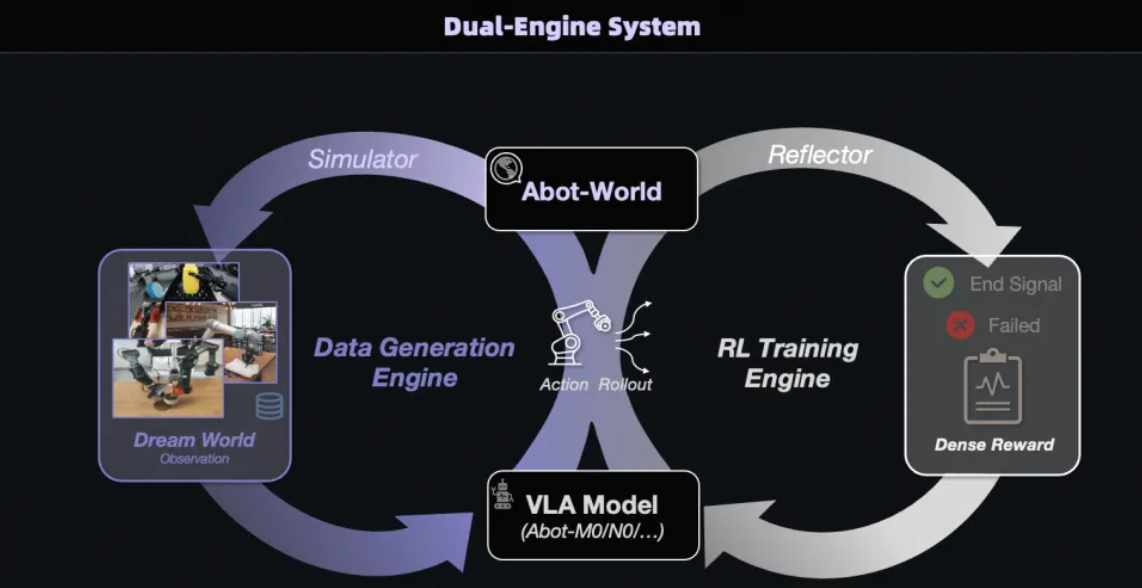
\includegraphics{images/image-0056.png}
\caption{ABot-World 双引擎系统}
\end{figure}

\hypertarget{ux4e8cux4e16ux754cux6a21ux578bux4e0eux7b56ux7565ux6a21ux578bux7684ux95edux73af}{%
\subsubsection{（二）世界模型与策略模型的闭环}\label{ux4e8cux4e16ux754cux6a21ux578bux4e0eux7b56ux7565ux6a21ux578bux7684ux95edux73af}}

ABot-World不是一个静态模型，而是一个具备自我修正能力的认知基座，能接入真实世界的执行反馈，让自己越用越准。VLA和世界模型构成完整的闭环（预测---执行---反馈---自我修正）。例如，机器人根据ABot-World的推演去抓杯子，结果实际执行中夹爪滑脱了。这个误差信号会立刻回传给ABot-PhysWorld，模型自动调整参数，下次预测就会更精准。闭环工作流如下：

\begin{enumerate}
\def\labelenumi{\arabic{enumi}.}
\item
  预测：基于DiT架构，以当前观测和动作为输入，在潜空间中直接生成符合时空动力学的未来状态序列。
\item
  执行：将推演出的最优动作指令下发给机器人执行机构。
\item
  反馈：采集真实世界的执行结果（例如预测能抓起水杯，但实际机械夹爪滑脱了）。
\item
  自我修正：利用真实世界的误差信号反哺认知基座，实时调整模型权重或状态记忆，使得模型``越用越准''。
\end{enumerate}

\hypertarget{ux53c2ux8003ux6587ux732e-205}{%
\subsection{参考文献}\label{ux53c2ux8003ux6587ux732e-205}}

\begin{itemize}
\tightlist
\item
  Wang, R., Liu, Q., Deng, Y., Liu, G., Liu, Z., \& Jia, K. (2026). \href{https://arxiv.org/abs/2603.17808}{EVA: Aligning Video World Models with Executable Robot Actions via Inverse Dynamics Rewards}. arXiv:2603.17808.
\item
  Chen, Y., Chen, R., Huo, D., Yang, Y., Qi, D., Liu, H., Lin, T., Zeng, S., Xiao, J., Chang, X., Xiong, F., Wei, X., Ma, Z., \& Xu, M. (2026). \href{https://arxiv.org/abs/2603.23376}{ABot-PhysWorld: Interactive World Foundation Model for Robotic Manipulation with Physics Alignment}. arXiv:2603.23376.
\end{itemize}

\clearpage

\hypertarget{ux4e16ux754c-ux7b56ux7565ux7edfux4e00ux67b6ux6784ux7684ux5177ux8eabux667aux80fdux8bbaux6587}{%
\section{世界-策略统一架构的具身智能（论文）}\label{ux4e16ux754c-ux7b56ux7565ux7edfux4e00ux67b6ux6784ux7684ux5177ux8eabux667aux80fdux8bbaux6587}}

\begin{quote}
本文是论文阅读笔记，内容代表对对应论文方法或作者理解，不应直接视为领域共识或工程最佳实践。
\end{quote}

\hypertarget{ux4e00ux57faux4e8eux4e16ux754cux6a21ux578bux7684ux5faeux8c03}{%
\subsection{一、基于世界模型的微调}\label{ux4e00ux57faux4e8eux4e16ux754cux6a21ux578bux7684ux5faeux8c03}}

基于具有对物理世界深刻认知的世界模型进行微调，可以获得具身智能需要的``大脑''和训练环境。下面以宇树科技 UnifoLM-WMA-0 为例介绍。

\hypertarget{ux4e00ux5de5ux4f5cux6a21ux5f0f}{%
\subsubsection{（一）工作模式}\label{ux4e00ux5de5ux4f5cux6a21ux5f0f}}

UnifoLM-WMA-0 的核心在于让模型理解机器人与环境相互作用时的物理规律。为了实现这一目标，该架构被设计为支持两种独立但互补的核心工作模式：

\begin{enumerate}
\def\labelenumi{\arabic{enumi}.}
\tightlist
\item
  \textbf{决策模式（Decision-Making Mode / Policy Enhancement）}：执行任务时，世界模型会提前预测机器人在给定动作下与环境物理交互的未来关键信息。这些具有物理常识的``未来特征''，例如物体形变和位移预判，会被输入到动作策略头中，辅助机器人生成更精确的下一步动作。
\item
  \textbf{仿真模式（Simulation Mode / Simulation Engine）}：模型作为交互式物理仿真器运行。输入机器人给定的动作指令后，模型能够自回归地生成高度还原真实场景的物理环境反馈，通常表现为未来视频帧。这相当于在神经网络内部为机器人构建一个可交互的``梦境''环境，可用于生成合成数据以强化学习。
\end{enumerate}

\hypertarget{ux4e8cux6838ux5fc3ux67b6ux6784ux548cux5de5ux4f5cux6d41}{%
\subsubsection{（二）核心架构和工作流}\label{ux4e8cux6838ux5fc3ux67b6ux6784ux548cux5de5ux4f5cux6d41}}

UnifoLM-WMA-0 的训练与部署工作流分为三个阶段，逐步从单纯的``视频生成''过渡到``物理决策''：

\begin{enumerate}
\def\labelenumi{\arabic{enumi}.}
\tightlist
\item
  \textbf{视频生成模型基础微调（World Model Pre-training）}

  \begin{itemize}
  \tightlist
  \item
    输入：海量跨实体机器人数据集（如 Open-X Embodiment Dataset）中的图像观测（Observation）和文本指令（Text Instruction）。
  \item
    处理：对预训练的视频生成扩散模型进行针对性微调，使其生成能力从``生成通用视频''收敛到``生成机器人真实作业场景视频''。
  \item
    输出：具备基础物理直觉的视频大模型。
  \end{itemize}
\item
  \textbf{决策模式后训练（Decision-making Post-training）}

  \begin{itemize}
  \tightlist
  \item
    输入：下游具体任务数据集，例如具体型号机器人的抓取、叠积木动作数据。
  \item
    处理：冻结部分世界模型参数，接入动作头（Action Head）。将世界模型提取的中间特征表征与环境观测共同喂入动作头。
  \item
    输出：优化动作头网络，使其能够输出精确的关节控制指令序列。
  \end{itemize}
\item
  \textbf{仿真模式后训练（Simulation Post-training）}

  \begin{itemize}
  \tightlist
  \item
    输入：当前环境观测、文本指令，以及给定动作序列（Action Condition）。
  \item
    处理：强迫世界模型不仅根据文本预测未来，还严格遵循输入动作序列生成对应的未来物理反馈视频。
  \item
    输出：高保真的交互式神经网络仿真器。
  \end{itemize}
\item
  基于机器人数据、图像和文本指令的基础微调。
\end{enumerate}

\textbf{子步骤 1：独立编码与降维压缩（Encoding \& Compression）}。高分辨率像素图像和离散自然语言文本无法直接在同一个数学空间中计算，因此第一步必须将它们映射到各自的高维连续特征空间中。

\textbf{图像观测处理（Image Observation Processing）}：为了大幅降低扩散模型的计算复杂度，系统通常不会在像素空间直接操作，而是使用预训练变分自编码器（VQ-VAE 或连续 VAE）的编码器模块。设输入的初始图像观测为高分辨率张量 \(o_0 \in \mathbb{R}^{H \times W \times 3}\)，经过编码器后，图像被压缩为隐空间特征图：

\[
z_0 = E(o_0), \qquad z_0 \in \mathbb{R}^{h \times w \times c}
\]

其中 \(h,w\) 是压缩后的空间分辨率，\(c\) 是隐通道数。此时 \(z_0\) 包含当前机器人视角下浓缩的几何与物理状态。

\textbf{文本指令处理（Text Instruction Processing）}：输入的自然语言指令，例如``将红色苹果放入篮子中''，由大语言模型或文本编码器（如 T5 或 CLIP Text Encoder）分词并提取语义特征，转化为上下文嵌入序列：

\[
E_{\mathrm{text}} = T(c_{\mathrm{text}}), \qquad E_{\mathrm{text}} \in \mathbb{R}^{L \times D}
\]

\textbf{子步骤 2：跨模态时空注意力融合（Cross-Modal Attention Fusion）}。扩散模型主干网络通常是 3D U-Net 或 Diffusion Transformer（DiT），它需要把``文本的意思''和``图像的现状''融合进未来画面的生成过程。网络内部主要通过交叉注意力机制实现文本指令对视觉生成的指导。设网络当前层处理的未来视频帧隐变量特征为 \(z_{\mathrm{visual}}\)，则：

\[
Q = W_Q z_{\mathrm{visual}}
\]

\[
K = W_K E_{\mathrm{text}}, \qquad V = W_V E_{\mathrm{text}}
\]

物理解释是：当网络生成``机械臂抓取苹果''的画面时，画面中``机械臂''和``苹果''所在区域的视觉特征会与文本指令中``抓取''和``苹果''的语义向量产生高权重匹配，从而使生成的视频遵循文本约束。

\textbf{子步骤 3：基于条件的隐空间去噪（Conditional Denoising）}。融合图像观测 \(z_0\) 和文本指令 \(E_{\mathrm{text}}\) 后，模型以它们为条件预测未来视频序列噪声。假设预测未来第 \(k\) 帧的隐状态，网络接收加噪的未来隐状态 \(z_t^{(k)}\)，并以拼接或自注意力方式注入初始观测 \(z_0\)。网络相关目标函数可写为：

\[
\mathcal{L}
= \mathbb{E}_{\epsilon \sim \mathcal{N}(0,1), t}
\left[
\left\|
\epsilon - \epsilon_\theta \left(z_t^{(k)}, k, z_0, E_{\mathrm{text}}\right)
\right\|_2^2
\right]
\]

通过优化这一损失，模型学习``看到初始画面 \(z_0\)，并听到指令 \(E_{\mathrm{text}}\) 时，接下来的物理世界应该如何演变''。

\begin{enumerate}
\def\labelenumi{\arabic{enumi}.}
\setcounter{enumi}{1}
\tightlist
\item
  决策模式。
\end{enumerate}

在决策模式下，目标是输出动作 \(a_{\mathrm{pred}}\)。系统会提取世界模型在逆向去噪过程中的中间层特征表示：

\[
f_{\mathrm{WM}}(o_t, c)
\]

这组特征隐含模型对场景几何和动力学规律的高维理解。动作策略头接收该特征，并输出对应动作。对于连续型物理控制任务，采用均方误差（MSE）计算与专家真实动作 \(a_{\mathrm{GT}}\) 的行为克隆损失：

\[
\mathcal{L}_{\mathrm{action}}
= \mathbb{E}_{o_t,c}
\left[
\left\|
a_{\mathrm{GT}} - \pi_\theta(f_{\mathrm{WM}}(o_t,c))
\right\|_2^2
\right]
\]

端到端联合微调时，系统总损失为：

\[
\begin{aligned}
\mathcal{L}_{\mathrm{total}}
&= \lambda_1 \mathcal{L}_{\mathrm{WM}}
\\
&\quad + \lambda_2 \mathcal{L}_{\mathrm{action}}
\end{aligned}
\]

\begin{enumerate}
\def\labelenumi{\arabic{enumi}.}
\setcounter{enumi}{2}
\tightlist
\item
  仿真模式：采用条件扩散模型的损失。
\end{enumerate}

\hypertarget{ux4e8clingbot-vaux57faux4e8e-mot-ux7684ux7b56ux7565ux4e0eux4e16ux754cux6a21ux578bux7edfux4e00}{%
\subsection{二、LingBot-VA：基于 MoT 的策略与世界模型统一}\label{ux4e8clingbot-vaux57faux4e8e-mot-ux7684ux7b56ux7565ux4e0eux4e16ux754cux6a21ux578bux7edfux4e00}}

在具身智能中，世界模型和 VLM/VLA 模型可以合二为一，采用 MoT 架构。下面以 LingBot-VA 为例分析。

\hypertarget{ux4e00ux987aux5e8fux53ccux6d41ux67b6ux6784}{%
\subsubsection{（一）顺序双流架构}\label{ux4e00ux987aux5e8fux53ccux6d41ux67b6ux6784}}

视觉观察首先通过因果视频 VAE 被压缩为紧凑隐变量 \(z_t \in \mathbb{R}^{N \times 4}\)。动作向量也被投影为对应维度的 token。在每个自回归步骤中，模型首先基于观察和动作历史，预测未来 \(K\) 帧视频画面的隐状态：

\[
z_{t+1:t+K} \sim p_\theta(z \mid z_{\le t}, a_{\lt t})
\]

随后，逆动力学模型利用预测的未来视觉状态、历史观察和历史动作，解码出具体动作：

\[
a_{t:t+K-1} \sim q_\phi(a \mid z_{t+1:t+K}, z_{\le t}, a_{\lt t})
\]

需要注意的是，上面的世界模型条件是 \(a_{\lt t}\) 而不是 \(a_{\le t}\)。这是因为第一阶段预测未来画面，第二阶段的逆动力学才根据预测画面推导当前应执行的动作 \(a_t\)。

视频流非常庞大，基于 Wan2.2-5B 预训练模型初始化，隐藏层维度高达 \(d_v=3072\)，因为它需要理解复杂视觉场景和物理动态。动作流则更轻量，深度虽与视频流相同，但隐藏层维度仅为 \(d_a=768\)，约为视频流的四分之一。这是因为动作分布，例如机械臂 7 自由度关节角和 1 维夹爪操作，在本质上比像素级视觉画面简单得多。

在世界模型中，这两个流融合在统一 Transformer 中推理。视频会被降采样，以保证 Transformer 维度对齐。在注意力层，两者统一交互：

\[
\left[z_t', a_{t,1}, a_{t,2}, \ldots, a_{t,r}, z_{t+1}', \ldots\right]
\]

在 MoT 结构中，两种模态通过交叉注意力机制融合特征，同时保持各自特征空间的独立性。

在前馈神经网络或 MoE 层，不同模态分开处理。二者的输出头也是分开的，但对每次输出 token 来说，总是只选择一个。输出时，模型可以在输出序列中交替输出视频 token 和动作 token。

\hypertarget{ux4e8cux5de5ux4f5cux6d41ux4e0eux5f02ux6b65ux63a8ux7406ux65b9ux6cd5}{%
\subsubsection{（二）工作流与异步推理方法}\label{ux4e8cux5de5ux4f5cux6d41ux4e0eux5f02ux6b65ux63a8ux7406ux65b9ux6cd5}}

整体是``块内扩散，块间自回归''，每个块包含 \(r\) 个 token。

\begin{enumerate}
\def\labelenumi{\arabic{enumi}.}
\tightlist
\item
  \textbf{基于 KV-Cache 的同步推理（Algorithm 1）}
\end{enumerate}

这是标准流程，利用大模型的 KV 缓存机制避免历史数据重复计算：

\begin{enumerate}
\def\labelenumi{\arabic{enumi}.}
\item
  获取初始图像 \(o_0\)，通过 VAE 编码为 \(z_0\)，将其存入缓存 \(C_0\)。
\item
  采样随机噪声，结合缓存 \(C\)，通过积分流时间至 \(s=0.5\)，生成未来的视频块预测 \(z_{t+1:t+K}\)。
\item
  基于预测出的视频块和缓存，积分流时间至 \(s=1.0\)，生成未来的动作块 \(a_{t:t+K-1}\)。
\item
  机器人执行动作，收集真实环境的新观察，并将新的 \(z\) 与 \(a\) 追加到缓存 \(C\) 中，循环执行。
\item
  \textbf{FDM-grounded 异步推理（Algorithm 2）}
\end{enumerate}

假设当前系统处于时间步 \(t\)：

\begin{itemize}
\tightlist
\item
  机器人侧：正在花费物理时间执行动作块 \(a_t\)。
\item
  模型侧：必须立刻开始计算下一时间步的动作 \(a_{t+1}\)，以保证 \(a_t\) 执行完后无缝衔接。
\item
  困境：此时现实世界中，执行 \(a_t\) 后的最终真实视觉状态尚未发生，相机无法捕捉。
\end{itemize}

如果采用朴素异步策略，模型会直接从 KV-Cache 里取上一轮在 \(t-1\) 时刻凭空预测出来的幻觉状态，并基于这个过期幻觉继续预测未来的 \(z_{t+1}\)。由于视频生成模型偏好时间平滑性，它会顺着幻觉轨迹一路生成下去，忽视现实世界中已经发生的微小物理偏差，最终导致开环退化和轨迹漂移。

为了打断这种``用幻觉预测幻觉''的恶性循环，系统会提取目前能拿到的最新真实环境反馈，也就是执行 \(a_{t-1}\) 之前的真实观测 \(z_{t-1}\)。

此时模型不使用旧预测，而是执行一次 FDM 前向传播。它将最新真实观测 \(z_{t-1}\) 以及当前电机正在执行的动作 \(a_t\) 一起喂给模型，让模型在真实前置条件下推演``施加该动作后，当前视觉状态应该变成什么样''，得到新的 \(\hat{z}_t\)。

这一步是纠正的核心：系统将这个基于真实数据反馈推演出的 \(\hat{z}_t\) 强制更新进 KV-Cache，替换原本陈旧、未接地的预测。随后，模型基于这个与环境反馈重新对齐的基础，再预测未来的视频块 \(z_{t+1}\) 并解码后续动作序列 \(a_{t+1}\)。

\hypertarget{ux4e09ux4e3aux4ec0ux4e48ux89c6ux89c9ux6d41ux53eaux9700ux8981ux53bbux566aux5230-s0.5ux52a8ux4f5cux6d41ux5fc5ux987bux5230-s1}{%
\subsubsection{\texorpdfstring{（三）为什么视觉流只需要去噪到 \(s=0.5\)，动作流必须到 \(s=1\)？}{（三）为什么视觉流只需要去噪到 s=0.5，动作流必须到 s=1？}}\label{ux4e09ux4e3aux4ec0ux4e48ux89c6ux89c9ux6d41ux53eaux9700ux8981ux53bbux566aux5230-s0.5ux52a8ux4f5cux6d41ux5fc5ux987bux5230-s1}}

简单来说，前者是为了加速，后者是为了精确。

\begin{enumerate}
\def\labelenumi{\arabic{enumi}.}
\tightlist
\item
  \textbf{视觉流}
\end{enumerate}

在自回归生成中，视频画面维度极高，生成视频 token 并进行多步去噪是推理过程最大的延迟来源。作者发现，逆动力学模型并不需要像素级完美的未来画面。只要视频画面能呈现大致的语义结构和运动趋势，动作解码器就能提取足够信息来规划动作。

为让模型具备``看半成品做决策''的能力，训练阶段以 \(p=0.5\) 的概率将历史视觉特征 \(z_{\lt t}\) 替换为部分加噪特征 \(\tilde{z}_{\lt t}\)：

\[
\tilde{z}_{\lt t} = (1-s_{\mathrm{aug}})z_{\lt t} + s_{\mathrm{aug}}\epsilon,
\qquad s_{\mathrm{aug}} \in [0.5, 1]
\]

这里的 \(s_{\mathrm{aug}}\) 模拟未完全去噪状态。通过这种增强，动作解码器被训练出从半模糊视频状态中准确预测动作的鲁棒性。

因此，在实际推理时，视频流不必完全去噪到 \(s=1\)。只需将常微分方程（ODE）积分到 \(s=0.5\)，有些实现中具体到 \(s=0.6\)，即可把半噪声的视频块交给后续动作流使用。这会显著降低视频生成的去噪步数和计算开销。

\begin{enumerate}
\def\labelenumi{\arabic{enumi}.}
\setcounter{enumi}{1}
\tightlist
\item
  \textbf{动作流}
\end{enumerate}

半模糊视频可以看懂，但半噪声动作无法在物理世界中执行。机器人的动作空间包含末端位姿、旋转四元数、关节角度和夹爪开合等连续数值，任何残余噪声都可能造成碰撞或抓取失败。因此动作流必须完整积分到 \(s=1.0\)，获得干净、确定的动作指令。

得益于非对称 MoT 架构，动作流隐藏层维度较低，仅为视频流宽度的四分之一，参数量也小。对低维动作数据进行完整 ODE 积分的额外计算开销很小，不会像视频生成那样成为系统瓶颈。

\hypertarget{ux4e09ux7269ux7406-token-ux7684ux7edfux4e00ux81eaux56deux5f52ux9884ux6d4b}{%
\subsection{三、物理 token 的统一自回归预测}\label{ux4e09ux7269ux7406-token-ux7684ux7edfux4e00ux81eaux56deux5f52ux9884ux6d4b}}

PAR、PhysGen 等论文以及 NVIDIA DreamDojo 提出了把状态与策略统一编码到``物理 token''中，统一自回归生成，再在下游解码为状态与策略输出的范式。

\hypertarget{ux4e00ux6838ux5fc3ux601dux60f3-28}{%
\subsubsection{（一）核心思想}\label{ux4e00ux6838ux5fc3ux601dux60f3-28}}

将过去的视频和动作编码为统一物理 token。设 \(t\) 时刻的视频帧 token 集合为 \(o_t\)，动作 token 集合为 \(a_t\)，则上下文序列为：

\[
\left[\mathrm{prompt}, o_1, a_1, o_2, a_2, \ldots, o_t, a_t\right]
\]

模型联合预测下一步的 \([o_{t+1}, a_{t+1}]\)。预测出的 \([o_{t+1}, a_{t+1}]\) 再通过扩散解码，分别得到连续的未来状态值（视频）和要采取的动作值。

具体而言，\(o_t\) 和 \(a_t\) 的生成方式并不相同：\(o_t\) 内部 token 可以并行生成，\(a_t\) 内部则按时间顺序严格串行。借助 multi-token prediction，模型在动作块内部拉长微观规划视野，即使需要预判 2 到 5 步极小的机械臂位姿变化，也能让自回归生成的动作轨迹更连贯，避免控制上的短视和抖动。

\begin{figure}[htbp]
\centering
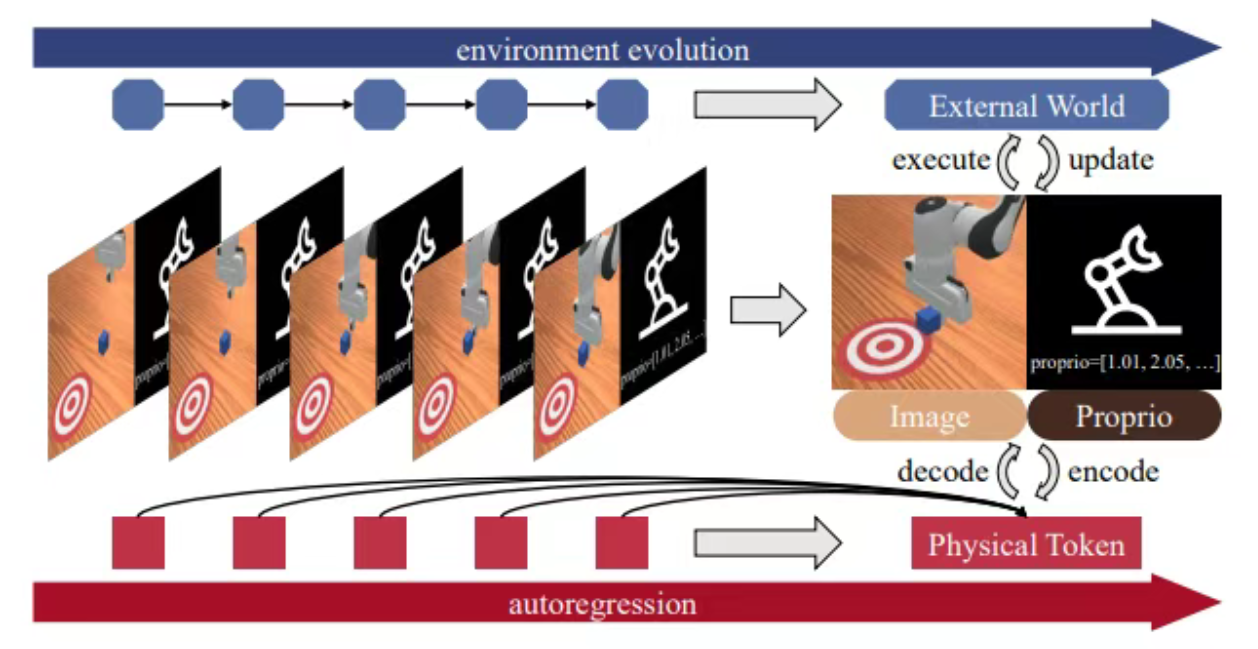
\includegraphics{images/image-0057.png}
\caption{PhysGen 物理 token 自回归示意图}
\end{figure}

\hypertarget{ux4e8cux81eaux56deux5f52-transformer}{%
\subsubsection{（二）自回归 Transformer}\label{ux4e8cux81eaux56deux5f52-transformer}}

主干 Transformer 网络采用自回归生成范式，因果掩码方式如下。

\begin{enumerate}
\def\labelenumi{\arabic{enumi}.}
\tightlist
\item
  \textbf{帧内部：块级全注意力}
\end{enumerate}

对于物理 token 中的视频帧部分，掩码允许同一画面内的所有图像块相互可见。单帧图像内部的空间信息是同时存在的，没有时间先后顺序。全注意力机制可以保证模型完整提取该帧全局空间特征。

\begin{enumerate}
\def\labelenumi{\arabic{enumi}.}
\setcounter{enumi}{1}
\tightlist
\item
  \textbf{动作内部：时间因果注意力}
\end{enumerate}

对于物理标记中的动作部分，模型执行严格的时间因果掩码。一个时间步的动作块内部，各个 token 仍有先后顺序，靠前动作标记不能关注排在后面的动作标记。这对应``过去决定未来，未来不能干涉过去''的物理约束。

\begin{enumerate}
\def\labelenumi{\arabic{enumi}.}
\setcounter{enumi}{2}
\tightlist
\item
  \textbf{动作单向关注视觉}
\end{enumerate}

在同一个时间步 \(t\) 中，动作 token 被允许单向关注视频 token。这使模型学习``给定目标状态，反推动作''的逆运动学推导。

\begin{enumerate}
\def\labelenumi{\arabic{enumi}.}
\setcounter{enumi}{3}
\tightlist
\item
  \textbf{跨时间步：全局时间因果}
\end{enumerate}

不同时间步之间严格遵守时间因果掩码，用 \(t\) 时刻以前的信息预测 \(t+1\) 时刻，防止未来帧信息泄露到过去规划中。

\hypertarget{ux4e09ux6269ux6563ux89e3ux7801ux5668}{%
\subsubsection{（三）扩散解码器}\label{ux4e09ux6269ux6563ux89e3ux7801ux5668}}

与传统离散分类不同，PhysGen 引入基于 DiT（Diffusion Transformer）的去噪过程，利用扩散损失直接在连续空间中估计概率分布。模型被训练来预测注入噪声，从而最小化均方误差损失：

\[
\begin{aligned}
\mathcal{L}(P_n, z_n)
&= \mathbb{E}_{\epsilon,t}
\left[
\left\|
\epsilon - \epsilon_\theta(P_{n,t}\mid t,z_n)
\right\|_2^2
\right]
\end{aligned}
\]

推理阶段去噪公式为：

\[
\begin{aligned}
P_{n,t-1}
&=
\frac{1}{\sqrt{\alpha_t}}
\left(
P_{n,t}
\, - \, \frac{1-\alpha_t}{\sqrt{1-\bar{\alpha}_t}}
\epsilon_\theta(P_{n,t}\mid t,z_n)
\right)
\\
&\quad + \sigma_t \epsilon
\end{aligned}
\]

去噪后的物理标记最终被分离，并解码为预测视频帧和真实世界中要执行的机器人动作。

\hypertarget{ux56dbboa-token}{%
\subsubsection{（四）BOA token}\label{ux56dbboa-token}}

真实物理世界中的因果关系非常严格。假设一个机器人需要完成任务：

\begin{itemize}
\tightlist
\item
  初始时刻 \(t=0\)：机器人看到桌子上的杯子，获得初始视觉观察结果 Frame 0，但此时还没有执行任何动作。
\item
  第一步 \(t=1\)：机器人处理 Frame 0 的信息，决定伸出机械臂并输出第一个动作 Action 1。因为这个动作，物理世界发生变化，机器人看到新的画面 Frame 1。
\end{itemize}

PhysGen 的特色是把帧标记（Frame token）和动作标记（Action token）拼在一起，组成统一的物理标记 \(P_n\) 来进行自回归预测：

\[
P_n = [F_{o,n}; F_{a,n}]
\]

按照物理直觉，输入模型的历史序列是：

\begin{itemize}
\tightlist
\item
  视觉观察序列：\(\{O_0,O_1,O_2,\ldots,O_{N-1}\}\)，从 0 开始，多一个初始帧。
\item
  对应动作序列：\(\{A_1,A_2,\ldots,A_{N-1}\}\)，从 1 开始，少一个初始动作。
\end{itemize}

如果强行两两打包，就会遇到时间偏移问题：

\begin{itemize}
\tightlist
\item
  \(P_0 = [O_0; \varnothing]\)，这里对不齐。
\item
  \(P_1 = [O_1; A_1]\)
\item
  \(P_2 = [O_2; A_2]\)
\end{itemize}

为在数学结构上对齐这两个长度不同的序列，让它们能放入 Transformer，作者在动作序列最前面人为塞入一个可学习占位符，称为 BOA（Begin of Action）token。

\hypertarget{ux4e94ux8badux7ec3ux5de5ux4f5cux6d41}{%
\subsubsection{（五）训练工作流}\label{ux4e94ux8badux7ec3ux5de5ux4f5cux6d41}}

\begin{enumerate}
\def\labelenumi{\arabic{enumi}.}
\tightlist
\item
  \textbf{预训练}
\end{enumerate}

预训练阶段，模型主干网络只在海量视频数据上训练。此时模型尚未见过机器人动作指令，学习的是``世界如何运转''，例如杯子掉到地上会碎、手碰到物体会让物体移动等物理和时间动态。

该阶段只训练语言 tokenizer、视觉 tokenizer（如 D-VAE）、自回归 Transformer 主干以及帧生成器（Frame Diffusion），动作模块不参与。

\begin{enumerate}
\def\labelenumi{\arabic{enumi}.}
\setcounter{enumi}{1}
\tightlist
\item
  \textbf{动作微调}
\end{enumerate}

为了让模型控制机器人，作者会在具体下游任务上进行微调（Fine-tuning）。这一阶段使用带动作标签的演示数据。因为模型在第一阶段已经学习到物理世界运作规律，所需动作数据量可以较小。

此时模型会增加用于编码动作的 Action Tokenizer（一个 MLP）以及轻量级动作解码器（Action-DiT）。微调时，模型被训练为：一旦看到 BOA token，后续就按``60 个视频帧 token + 8 个动作 token''的模式交替生成，系统再按 token 类型分发给不同解码器。

\hypertarget{ux53c2ux8003ux6587ux732e-206}{%
\subsection{参考文献}\label{ux53c2ux8003ux6587ux732e-206}}

\begin{itemize}
\tightlist
\item
  Unitree Robotics. (2025). \href{https://github.com/unitreerobotics/unifolm-world-model-action}{UnifoLM-WMA-0: World-Model-Action Architecture for General Robots}. GitHub repository.
\item
  Li, L., Zhang, Q., Yu, M., Gao, Z., Luo, Y., Xue, N., Yang, S., Zhu, X., Wang, R., Shen, Y., Han, F., \& Xu, Y. (2026). \href{https://arxiv.org/abs/2601.21998}{Causal World Modeling for Robot Control}. arXiv:2601.21998.
\end{itemize}

\clearpage

\hypertarget{ux4ec5ux5728ux8badux7ec3ux65f6ux878dux5165ux9884ux6d4bux80fdux529bux7684ux5177ux8eabux667aux80fdux8bbaux6587}{%
\section{仅在训练时融入预测能力的具身智能（论文）}\label{ux4ec5ux5728ux8badux7ec3ux65f6ux878dux5165ux9884ux6d4bux80fdux529bux7684ux5177ux8eabux667aux80fdux8bbaux6587}}

\begin{quote}
本文是论文阅读笔记，内容代表对对应论文方法或作者理解，不应直接视为领域共识或工程最佳实践。
\end{quote}

\hypertarget{ux4e00fast-wamux4ec5ux5728ux8badux7ec3ux65f6ux9884ux6d4bux72b6ux6001ux7684ux63a8ux7406}{%
\subsection{一、Fast-WAM：仅在训练时预测状态的推理}\label{ux4e00fast-wamux4ec5ux5728ux8badux7ec3ux65f6ux9884ux6d4bux72b6ux6001ux7684ux63a8ux7406}}

\hypertarget{ux4e00ux95eeux9898ux80ccux666f-22}{%
\subsubsection{（一）问题背景}\label{ux4e00ux95eeux9898ux80ccux666f-22}}

在具身智能领域，视觉-语言-动作模型（VLA, Vision-Language-Action），例如 OpenVLA、RT-2 等，在过去取得了巨大进展。然而，传统 VLA 主要基于静态图文数据进行预训练，缺乏对物理世界动态演变过程的建模。

为了解决这一问题，AI 领域发展出一条新的技术路线：世界动作模型（WAMs, World Action Models）。WAMs 将``预测未来视觉画面''与``预测机器人动作''结合在统一框架中，使模型具备物理先验知识。

现有 WAMs 大多遵循``先想象，后执行''（imagine-then-execute）的范式：推理时，模型必须先生成未来视频帧，再基于这些预测未来画面输出动作。该范式的致命弱点是推理延迟高。测试时需要通过扩散模型迭代去噪生成视频，使模型很难在机器人上实现低延迟实时控制。

因此，Fast-WAM 提出核心问题：WAMs 是否真的需要在测试时显式``想象''未来画面？还是说，性能提升主要来自训练阶段的视频预测协同训练（Video Co-training），它让模型学到了更好的物理世界表征？

\hypertarget{ux4e8cux57faux5ea7ux6a21ux578b}{%
\subsubsection{（二）基座模型}\label{ux4e8cux57faux5ea7ux6a21ux578b}}

Fast-WAM 采用开源视频扩散 Transformer Wan2.2-5B 作为世界建模骨干网络，复用 Wan2.2 的视频 DiT、文本编码器 T5 以及视频 VAE。

\hypertarget{ux4e09ux6a21ux578bux67b6ux6784ux4e0eux8badux7ec3ux5de5ux4f5cux6d41}{%
\subsubsection{（三）模型架构与训练工作流}\label{ux4e09ux6a21ux578bux67b6ux6784ux4e0eux8badux7ec3ux5de5ux4f5cux6d41}}

\textbf{第一步：Token 的精确分组}。在送入 MoT 架构前，所有输入信息被严格划分为三个 token 组：

\begin{enumerate}
\def\labelenumi{\arabic{enumi}.}
\tightlist
\item
  视觉锚点 \(f_0\)：当前第一帧观测图像的干净潜在特征，不加噪。
\item
  未来视频 \(f_{1:h}\)：未来视频帧的加噪潜在特征，仅在训练时存在。
\item
  动作序列 \(a_{1:h}\)：要生成的动作块的加噪特征。
\end{enumerate}

这里的``第一帧''是相对于原本要生成的未来视频块而言的锚点（Anchor）。模型摒弃了推理时生成未来画面的过程，而是将唯一一帧当前图像输入视频骨干网络做一次单向前向传播，提取世界表征，然后直接交给动作专家网络生成后续动作序列。这种设计使 Fast-WAM 具备类似标准 VLA 的快速实时响应能力。

\textbf{第二步：全局文本 Cross-Attention 注入}。在这三个 token 组进入 DiT 每一层时，所有 token 组都会通过 Cross-Attention 关注语言特征向量。数学上，\(f_0\)、\(f_{1:h}\) 和 \(a_{1:h}\) 都作为 Query，文本特征作为 Key 和 Value。其物理意义是：无论提取当前视觉特征、推演未来物理变化，还是规划具体动作，都始终受到人类语言指令引导。

\textbf{第三步：结构化 Self-Attention 掩码}。注入文本信息后，token 之间需要在 DiT 内部进行自注意力交互。作者设计严格注意力掩码来控制信息流：

\begin{itemize}
\tightlist
\item
  Video DiT 内部交互：未来加噪视频 token \(f_{1:h}\) 可以在视频分支内双向互相关注，并允许关注第一帧干净特征 \(f_0\)，使模型基于初始状态推演未来。
\item
  Action DiT 内部交互：动作 token \(a_{1:h}\) 可以在动作分支内双向互相关注，同样允许关注第一帧干净特征 \(f_0\)，使模型基于当前视觉状态规划连贯动作序列。
\item
  不可跨越的红线：动作 token 绝对不允许关注未来视频 token；同时，第一帧干净 token \(f_0\) 不关注任何其他 token，避免被噪声污染。
\end{itemize}

严禁越界的原因是：如果训练时动作特征能看到未来视频特征，动作专家会产生依赖，根据``未来已经发生的结果''反推``现在该做什么动作''。但在真实部署时，为追求约 190 毫秒的低延迟，Fast-WAM 会直接移除未来视频生成分支。若模型训练时依赖未来视频，推理时就会因输入缺失而崩溃。因此，结构化掩码强迫动作预测只能立足当前帧和文本，从根本上解耦训练时视频辅助和推理时动作生成。

\hypertarget{ux56dbux635fux5931ux51fdux6570-3}{%
\subsubsection{（四）损失函数}\label{ux56dbux635fux5931ux51fdux6570-3}}

对于目标变量 \(y\)，它既可以是动作序列 \(a_{1:h}\)，也可以是未来视频特征 \(z_{1:T}\)。算法采样高斯噪声 \(\epsilon \sim \mathcal{N}(0,I)\) 和时间步 \(t \in (0,1)\)，构建插值样本：

\[
y_t = (1-t)y + t\epsilon
\]

模型通过标准流匹配损失预测速度场：

\[
\begin{aligned}
\mathcal{L}_{\mathrm{FM}}(y)
&= \mathbb{E}_{y,\epsilon,t}
\left[
\left\|
f_\theta(y_t,t,o,l) - (\epsilon-y)
\right\|_2^2
\right]
\end{aligned}
\]

总优化目标是动作损失和视频协同训练损失的加权和：

\[
\begin{aligned}
\mathcal{L}
&= \mathcal{L}_{\mathrm{act}}
\\
&\quad + \lambda \mathcal{L}_{\mathrm{vid}}
\end{aligned}
\]

\hypertarget{ux4e94ux63a8ux7406ux5de5ux4f5cux6d41-1}{%
\subsubsection{（五）推理工作流}\label{ux4e94ux63a8ux7406ux5de5ux4f5cux6d41-1}}

推理阶段彻底抛弃显式视频生成，实现极快响应：

\begin{enumerate}
\def\labelenumi{\arabic{enumi}.}
\tightlist
\item
  \textbf{单次前向传递}：仅保留第一帧干净潜在特征，将其输入视频骨干网络进行一次单向前向传播，提取具有物理意义的潜在世界表征 \(z(o,l)\)。
\item
  \textbf{直接动作去噪}：动作专家 DiT 直接基于该表征参数化动作分布：
\end{enumerate}

\[
p_\theta(a_{1:H}\mid z(o,l))
\]

\begin{enumerate}
\def\labelenumi{\arabic{enumi}.}
\setcounter{enumi}{2}
\tightlist
\item
  \textbf{输出执行}：由于不需要对未来视频帧实例化和去噪，动作生成仅需少量无分类器引导（CFG=1.0）的去噪步即可输出动作序列。
\end{enumerate}

\hypertarget{ux516dux5b9eux9a8cux7ed3ux679c}{%
\subsubsection{（六）实验结果}\label{ux516dux5b9eux9a8cux7ed3ux679c}}

\begin{enumerate}
\def\labelenumi{\arabic{enumi}.}
\tightlist
\item
  \textbf{极低推理延迟}：真实机器人任务中，Fast-WAM 延迟约 190 毫秒，而采用``先想象后执行''的 Fast-WAM-IDM 延迟高达约 810 毫秒，Fast-WAM 实现超过 4 倍提速。
\item
  \textbf{性能接近前沿方法}：在没有进行大规模具身预训练（Embodied Pretraining）的情况下，Fast-WAM 在 RoboTwin 上取得 91.8\% 的成功率，在 LIBERO 上取得 97.6\% 的平均成功率，不仅优于不带视频预测的 VLA 基线，也接近最强预训练 WAMs。
\item
  \textbf{回答核心假设}：Fast-WAM 的表现与显式生成未来的变体（Joint 和 IDM）非常接近。但如果移除训练时的视频协同训练任务（w.o. video co-train），RoboTwin 成功率下降到 83.8\%，真机折叠毛巾任务成功率也显著下降。
\end{enumerate}

最终结论：WAMs 强大的根本原因在于训练阶段的视频预测任务重塑了模型的物理世界表征能力，而不在于推理阶段显式生成未来画面。Fast-WAM 说明，可以在训练时利用世界模型带来的物理先验，在部署时仍保持 VLA 式的快速响应。

\hypertarget{ux4e8cbeing-h0.7ux8badux7ec3ux65f6ux8ba9ux52a8ux4f5cux9884ux6d4bux4e0eux57faux4e8eux672aux6765ux72b6ux6001ux7684ux52a8ux4f5cux9884ux6d4bux5bf9ux9f50}{%
\subsection{二、Being-H0.7：训练时让``动作预测''与``基于未来状态的动作预测''对齐}\label{ux4e8cbeing-h0.7ux8badux7ec3ux65f6ux8ba9ux52a8ux4f5cux9884ux6d4bux4e0eux57faux4e8eux672aux6765ux72b6ux6001ux7684ux52a8ux4f5cux9884ux6d4bux5bf9ux9f50}}

\hypertarget{ux4e00ux95eeux9898ux80ccux666f-23}{%
\subsubsection{（一）问题背景}\label{ux4e00ux95eeux9898ux80ccux666f-23}}

具身大模型主要有两条技术路线，但均存在明显局限：

\begin{enumerate}
\def\labelenumi{\arabic{enumi}.}
\tightlist
\item
  \textbf{VLA（视觉-语言-动作模型）}：这类模型如 RT-2、OpenVLA 等，将当前视觉和语言观察直接映射为底层控制动作。痛点是机器人动作数据稀疏且缺乏多样性，模型容易出现行为崩溃（behavior collapse），依赖表面统计相关性，而未学到基于物理规律、具有组合泛化能力的动作表征。
\item
  \textbf{WAM（世界-动作模型）}：基于视频生成模型构建，通过预测未来像素帧演变推断世界动态。痛点包括推理阶段实时生成未来视频帧带来极高计算延迟、像素预测瑕疵会传递到动作解码并导致长周期任务失败，以及训练成本较高。
\end{enumerate}

\hypertarget{ux4e8cux6838ux5fc3ux601dux60f3-8}{%
\subsubsection{（二）核心思想}\label{ux4e8cux6838ux5fc3ux601dux60f3-8}}

Being-H0.7 不需要在像素层面预测未来，而是在训练时让动作预测与基于未来状态的动作预测对齐。模型引入一组可学习的 Latent Queries，在 Transformer 前向传播中不断从多模态上下文中萃取任务相关信息，将其压缩重组并生成动作。训练时，模型还将观测到的未来状态压缩到 latent 空间，同样从多模态上下文中萃取任务相关信息并生成动作；然后让前者（先验分支）向后者（后验分支）对齐。

为了让推理空间真正具备``预测未来''的世界建模能力，作者设计训练期双分支联合对齐（Dual-Branch Joint Alignment）架构：

\begin{itemize}
\tightlist
\item
  \textbf{Prior Branch（先验分支）}：最终用于实机部署的干线分支，仅依赖当前指令和观察，使用 Latent Queries 生成动作。
\item
  \textbf{Posterior Branch（后验分支）}：仅存在于训练阶段的辅助分支，将干线中的 Latent Queries 替换为通过视觉编码器提取的未来观察嵌入（Future Embeddings）。
\item
  \textbf{对齐机制}：在隐藏层特征级别计算先验分支与后验分支的对齐损失，迫使先验分支在只看到当下画面时，推断出与``看到未来''相同的特征表示。
\end{itemize}

\hypertarget{ux4e09ux8badux7ec3ux5de5ux4f5cux6d41-4}{%
\subsubsection{（三）训练工作流}\label{ux4e09ux8badux7ec3ux5de5ux4f5cux6d41-4}}

\textbf{步骤 1：上下文编码与序列构建}。给定任务指令 \(x\)、时间长度为 \(H\) 的历史观测 \(O_{-H:0}\) 以及机器人本体状态 \(s\)。将这些特征映射并拼接后，算法在动作块 \(a_{0:T}\) 的预测序列前插入数量为 \(K\)、维度为 \(d\) 的潜在查询矩阵 \(Q \in \mathbb{R}^{K \times d}\)，构建先验分支的完整 Transformer 序列：

\[
S = \left[x; O_{-H:0}; s; Q; a_{0:T}\right]
\]

\textbf{步骤 2：后验分支的未来特征提取}。算法同步获取未来真实观测视频帧 \(O_{0:T}\)。使用冻结的预训练 ViT 和 Perceiver 重采样器 \(E\)，将其压缩成大小与 \(Q\) 一致的未来嵌入：

\[
z^{\mathrm{post}} = E(O_{0:T}) \in \mathbb{R}^{K \times d}
\]

\textbf{步骤 3：混合 Transformer（MoT）双分支前向传播}。为提高计算效率，算法不串行执行两次大型前向传播，而是利用 Mixture-of-Transformers 架构将两个分支打包成一个长序列。在这个过程中应用双分支注意力掩码（Dual-Branch Attention Mask）：保证两个分支都能看到共享上下文 \(c=[x;O_{-H:0};s]\)，但先验分支和后验分支的 tokens 彼此不可见。

\textbf{步骤 4：损失函数计算}。整个框架通过三个损失函数进行联合优化。

\begin{enumerate}
\def\labelenumi{\arabic{enumi}.}
\tightlist
\item
  \textbf{动作流匹配损失（Flow Matching Loss）}：基于扩散生成范式，为两个分支分别计算对加噪动作的去噪速度场损失。若真实动作为 \(a\)、加噪时间为 \(t\)、目标速度为 \(u_t=a-\epsilon\)，则：
\end{enumerate}

\[
\begin{aligned}
\mathcal{L}_{\mathrm{FM}}^{\mathrm{prior}}
&=
\left\|
v_\theta^{\mathrm{prior}}(a_t,c) - u_t
\right\|_2^2
\end{aligned}
\]

\[
\begin{aligned}
\mathcal{L}_{\mathrm{FM}}^{\mathrm{post}}
&=
\left\|
v_\theta^{\mathrm{post}}(a_t,c,z^{\mathrm{post}}) - u_t
\right\|_2^2
\end{aligned}
\]

\begin{enumerate}
\def\labelenumi{\arabic{enumi}.}
\setcounter{enumi}{1}
\tightlist
\item
  \textbf{隐状态联合对齐损失（Joint Alignment Loss）}：在第 \(l\) 个包含对齐的 Transformer 层，提取先验分支隐状态 \(h_l^{\mathrm{prior}}\) 与后验分支隐状态 \(h_l^{\mathrm{post}}\)，计算均方误差，促使先验空间涌现对未来的世界建模能力：
\end{enumerate}

\[
\begin{aligned}
\mathcal{L}_{\mathrm{align}}
&=
\frac{1}{L}
\sum_{l=1}^{L}
\left\|
h_l^{\mathrm{prior}} - h_l^{\mathrm{post}}
\right\|_2^2
\end{aligned}
\]

\begin{enumerate}
\def\labelenumi{\arabic{enumi}.}
\setcounter{enumi}{2}
\tightlist
\item
  \textbf{防崩溃正则化损失（Regularization Loss）}：为防止对齐导致隐特征趋于全 0 或方向单一化，施加范数和秩的惩罚。范数正则化防止幅值收缩：
\end{enumerate}

\[
\begin{aligned}
\mathcal{R}_{\mathrm{norm}}(h)
&=
\left[
\mathrm{ReLU}(\tau - \lVert h\rVert_2)
\right]^2
\end{aligned}
\]

秩正则化防止方向坍缩，由 Gram 矩阵 \(G\) 的归一化特征值 \(p_i\) 的信息熵表示：

\[
\begin{aligned}
\mathcal{R}_{\mathrm{rank}}(H)
&=
\sum_{i=1}^{B} p_i \log p_i
\end{aligned}
\]

\hypertarget{ux56dbux63a8ux7406ux5de5ux4f5cux6d41-1}{%
\subsubsection{（四）推理工作流}\label{ux56dbux63a8ux7406ux5de5ux4f5cux6d41-1}}

由于模型解耦了特征对齐和前向生成，推理阶段非常轻量：

\begin{enumerate}
\def\labelenumi{\arabic{enumi}.}
\tightlist
\item
  \textbf{观察采集}：机器人摄像头实时采集当前画面，处理并拼接为上下文向量。
\item
  \textbf{纯先验分支执行}：完全丢弃训练时的后验分支和所有未来视频输入，只保留 Transformer 骨干、Latent Queries \(Q\) 以及用于扩散的 Flow Matching 生成头。
\item
  \textbf{动作块输出与 UAC 异步控制}：模型一次性快速生成连续未来动作块 \(a_{0:T}\)。真实部署中结合通用异步分块机制（UAC）：服务器端异步推理未来动作序列，机器人驱动端从线程安全缓冲池中持续取出历史前缀锁定动作执行，两者解耦，以约 \(3\) 到 \(4\) ms/step 的低延迟实现平滑动态控制。
\end{enumerate}

\hypertarget{ux53c2ux8003ux6587ux732e-207}{%
\subsection{参考文献}\label{ux53c2ux8003ux6587ux732e-207}}

\begin{itemize}
\tightlist
\item
  Yuan, T., Dong, Z., Liu, Y., \& Zhao, H. (2026). \href{https://arxiv.org/abs/2603.16666}{Fast-WAM: Do World Action Models Need Test-time Future Imagination?}. arXiv:2603.16666.
\end{itemize}

\clearpage


\end{document}
